% Options for packages loaded elsewhere
\PassOptionsToPackage{unicode}{hyperref}
\PassOptionsToPackage{hyphens}{url}
\documentclass[
]{book}
\usepackage{xcolor}
\usepackage{amsmath,amssymb}
\setcounter{secnumdepth}{5}
\usepackage{iftex}
\ifPDFTeX
  \usepackage[T1]{fontenc}
  \usepackage[utf8]{inputenc}
  \usepackage{textcomp} % provide euro and other symbols
\else % if luatex or xetex
  \usepackage{unicode-math} % this also loads fontspec
  \defaultfontfeatures{Scale=MatchLowercase}
  \defaultfontfeatures[\rmfamily]{Ligatures=TeX,Scale=1}
\fi
\usepackage{lmodern}
\ifPDFTeX\else
  % xetex/luatex font selection
\fi
% Use upquote if available, for straight quotes in verbatim environments
\IfFileExists{upquote.sty}{\usepackage{upquote}}{}
\IfFileExists{microtype.sty}{% use microtype if available
  \usepackage[]{microtype}
  \UseMicrotypeSet[protrusion]{basicmath} % disable protrusion for tt fonts
}{}
\makeatletter
\@ifundefined{KOMAClassName}{% if non-KOMA class
  \IfFileExists{parskip.sty}{%
    \usepackage{parskip}
  }{% else
    \setlength{\parindent}{0pt}
    \setlength{\parskip}{6pt plus 2pt minus 1pt}}
}{% if KOMA class
  \KOMAoptions{parskip=half}}
\makeatother
\usepackage{color}
\usepackage{fancyvrb}
\newcommand{\VerbBar}{|}
\newcommand{\VERB}{\Verb[commandchars=\\\{\}]}
\DefineVerbatimEnvironment{Highlighting}{Verbatim}{commandchars=\\\{\}}
% Add ',fontsize=\small' for more characters per line
\usepackage{framed}
\definecolor{shadecolor}{RGB}{248,248,248}
\newenvironment{Shaded}{\begin{snugshade}}{\end{snugshade}}
\newcommand{\AlertTok}[1]{\textcolor[rgb]{0.94,0.16,0.16}{#1}}
\newcommand{\AnnotationTok}[1]{\textcolor[rgb]{0.56,0.35,0.01}{\textbf{\textit{#1}}}}
\newcommand{\AttributeTok}[1]{\textcolor[rgb]{0.13,0.29,0.53}{#1}}
\newcommand{\BaseNTok}[1]{\textcolor[rgb]{0.00,0.00,0.81}{#1}}
\newcommand{\BuiltInTok}[1]{#1}
\newcommand{\CharTok}[1]{\textcolor[rgb]{0.31,0.60,0.02}{#1}}
\newcommand{\CommentTok}[1]{\textcolor[rgb]{0.56,0.35,0.01}{\textit{#1}}}
\newcommand{\CommentVarTok}[1]{\textcolor[rgb]{0.56,0.35,0.01}{\textbf{\textit{#1}}}}
\newcommand{\ConstantTok}[1]{\textcolor[rgb]{0.56,0.35,0.01}{#1}}
\newcommand{\ControlFlowTok}[1]{\textcolor[rgb]{0.13,0.29,0.53}{\textbf{#1}}}
\newcommand{\DataTypeTok}[1]{\textcolor[rgb]{0.13,0.29,0.53}{#1}}
\newcommand{\DecValTok}[1]{\textcolor[rgb]{0.00,0.00,0.81}{#1}}
\newcommand{\DocumentationTok}[1]{\textcolor[rgb]{0.56,0.35,0.01}{\textbf{\textit{#1}}}}
\newcommand{\ErrorTok}[1]{\textcolor[rgb]{0.64,0.00,0.00}{\textbf{#1}}}
\newcommand{\ExtensionTok}[1]{#1}
\newcommand{\FloatTok}[1]{\textcolor[rgb]{0.00,0.00,0.81}{#1}}
\newcommand{\FunctionTok}[1]{\textcolor[rgb]{0.13,0.29,0.53}{\textbf{#1}}}
\newcommand{\ImportTok}[1]{#1}
\newcommand{\InformationTok}[1]{\textcolor[rgb]{0.56,0.35,0.01}{\textbf{\textit{#1}}}}
\newcommand{\KeywordTok}[1]{\textcolor[rgb]{0.13,0.29,0.53}{\textbf{#1}}}
\newcommand{\NormalTok}[1]{#1}
\newcommand{\OperatorTok}[1]{\textcolor[rgb]{0.81,0.36,0.00}{\textbf{#1}}}
\newcommand{\OtherTok}[1]{\textcolor[rgb]{0.56,0.35,0.01}{#1}}
\newcommand{\PreprocessorTok}[1]{\textcolor[rgb]{0.56,0.35,0.01}{\textit{#1}}}
\newcommand{\RegionMarkerTok}[1]{#1}
\newcommand{\SpecialCharTok}[1]{\textcolor[rgb]{0.81,0.36,0.00}{\textbf{#1}}}
\newcommand{\SpecialStringTok}[1]{\textcolor[rgb]{0.31,0.60,0.02}{#1}}
\newcommand{\StringTok}[1]{\textcolor[rgb]{0.31,0.60,0.02}{#1}}
\newcommand{\VariableTok}[1]{\textcolor[rgb]{0.00,0.00,0.00}{#1}}
\newcommand{\VerbatimStringTok}[1]{\textcolor[rgb]{0.31,0.60,0.02}{#1}}
\newcommand{\WarningTok}[1]{\textcolor[rgb]{0.56,0.35,0.01}{\textbf{\textit{#1}}}}
\usepackage{longtable,booktabs,array}
\usepackage{calc} % for calculating minipage widths
% Correct order of tables after \paragraph or \subparagraph
\usepackage{etoolbox}
\makeatletter
\patchcmd\longtable{\par}{\if@noskipsec\mbox{}\fi\par}{}{}
\makeatother
% Allow footnotes in longtable head/foot
\IfFileExists{footnotehyper.sty}{\usepackage{footnotehyper}}{\usepackage{footnote}}
\makesavenoteenv{longtable}
\usepackage{graphicx}
\makeatletter
\newsavebox\pandoc@box
\newcommand*\pandocbounded[1]{% scales image to fit in text height/width
  \sbox\pandoc@box{#1}%
  \Gscale@div\@tempa{\textheight}{\dimexpr\ht\pandoc@box+\dp\pandoc@box\relax}%
  \Gscale@div\@tempb{\linewidth}{\wd\pandoc@box}%
  \ifdim\@tempb\p@<\@tempa\p@\let\@tempa\@tempb\fi% select the smaller of both
  \ifdim\@tempa\p@<\p@\scalebox{\@tempa}{\usebox\pandoc@box}%
  \else\usebox{\pandoc@box}%
  \fi%
}
% Set default figure placement to htbp
\def\fps@figure{htbp}
\makeatother
\setlength{\emergencystretch}{3em} % prevent overfull lines
\providecommand{\tightlist}{%
  \setlength{\itemsep}{0pt}\setlength{\parskip}{0pt}}
\usepackage[]{natbib}
\bibliographystyle{apalike}
% LaTeX preamble for R Errors Book

% Better fonts
\usepackage{lmodern}
\usepackage[T1]{fontenc}

% Better code formatting
\usepackage{fancyvrb}
\usepackage{listings}

% Colors for code
\usepackage{xcolor}
\definecolor{codegray}{rgb}{0.95,0.95,0.95}
\definecolor{codegreen}{rgb}{0,0.6,0}
\definecolor{codepurple}{rgb}{0.58,0,0.82}

% Hyperlinks
\usepackage{hyperref}
\hypersetup{
    colorlinks=true,
    linkcolor=blue,
    filecolor=magenta,      
    urlcolor=cyan,
    pdftitle={R Errors and How to Fix Them},
    pdfauthor={},
    pdfsubject={R Programming},
    pdfkeywords={R, errors, debugging, programming},
}

% Better tables
\usepackage{booktabs}
\usepackage{longtable}

% Graphics
\usepackage{graphicx}

% Better spacing
\usepackage{microtype}

% Section formatting
\usepackage{titlesec}

% Page layout
\usepackage{geometry}
\geometry{
  margin=1in,
  includeheadfoot
}

% Headers and footers
\usepackage{fancyhdr}
\pagestyle{fancy}
\fancyhf{}
\fancyhead[LE,RO]{\thepage}
\fancyhead[LO]{\nouppercase{\rightmark}}
\fancyhead[RE]{\nouppercase{\leftmark}}

% Code blocks with background
\lstset{
  backgroundcolor=\color{codegray},
  basicstyle=\ttfamily\small,
  breaklines=true,
  frame=single,
  numbers=left,
  numberstyle=\tiny,
  captionpos=b
}

% Prevent overfull hbox warnings
\setlength{\emergencystretch}{3em}

% Better list spacing
\usepackage{enumitem}
\setlist{noitemsep}
\usepackage{bookmark}
\IfFileExists{xurl.sty}{\usepackage{xurl}}{} % add URL line breaks if available
\urlstyle{same}
\hypersetup{
  pdftitle={Mastering R Through Errors and Warnings},
  pdfauthor={Kai Guo},
  hidelinks,
  pdfcreator={LaTeX via pandoc}}

\title{Mastering R Through Errors and Warnings}
\usepackage{etoolbox}
\makeatletter
\providecommand{\subtitle}[1]{% add subtitle to \maketitle
  \apptocmd{\@title}{\par {\large #1 \par}}{}{}
}
\makeatother
\subtitle{A Comprehensive Guide to Learning R by Understanding What Goes Wrong}
\author{Kai Guo}
\date{2025-10-25}

\begin{document}
\maketitle

{
\setcounter{tocdepth}{1}
\tableofcontents
}
\chapter*{Welcome}\label{welcome}
\addcontentsline{toc}{chapter}{Welcome}

\section*{Why This Book Exists}\label{why-this-book-exists}
\addcontentsline{toc}{section}{Why This Book Exists}

\textbf{You will make errors in R. Lots of them.}

That's not a prediction---it's a promise. And it's exactly how learning works.

Most R books teach you how to do things \emph{right}. This book teaches you what happens when things go \emph{wrong}, because:

\begin{enumerate}
\def\labelenumi{\arabic{enumi}.}
\tightlist
\item
  \textbf{You learn more from errors than successes} - Each error is a teaching moment
\item
  \textbf{Errors reveal R's internal logic} - Understanding why something fails helps you understand how R thinks
\item
  \textbf{You'll spend more time debugging than writing new code} - Better to learn it systematically
\item
  \textbf{Error messages are often cryptic} - But they follow patterns once you know what to look for
\end{enumerate}

\section*{How This Book Works}\label{how-this-book-works}
\addcontentsline{toc}{section}{How This Book Works}

\subsection*{The Error-First Approach}\label{the-error-first-approach}
\addcontentsline{toc}{subsection}{The Error-First Approach}

Each chapter follows this structure:

\begin{enumerate}
\def\labelenumi{\arabic{enumi}.}
\tightlist
\item
  \textbf{Show the error/warning} - You'll see it in a red/yellow box
\item
  \textbf{Explain what causes it} - The underlying R behavior
\item
  \textbf{Demonstrate the solution} - Multiple approaches when applicable
\item
  \textbf{Provide practice problems} - Intentionally broken code for you to fix
\end{enumerate}

\subsection*{Organization System}\label{organization-system}
\addcontentsline{toc}{subsection}{Organization System}

We use visual indicators throughout:

\begin{itemize}
\tightlist
\item
  🔴 \textbf{ERROR}: Stops execution completely
\item
  🟡 \textbf{WARNING}: Continues but alerts you to potential issues
\item
  🔵 \textbf{MESSAGE}: Informational only
\item
  ✅ \textbf{SOLUTION}: The fix
\end{itemize}

\textbf{Difficulty Levels:}

\begin{itemize}
\tightlist
\item
  ⭐ Beginner - Everyone encounters these
\item
  ⭐⭐ Intermediate - Common with experience
\item
  ⭐⭐⭐ Advanced - Edge cases and complex scenarios
\end{itemize}

\textbf{Error Categories:}

\begin{itemize}
\tightlist
\item
  🔤 Syntax/Typo
\item
  📦 Package Issue
\item
  🔢 Type Mismatch
\item
  📏 Dimension/Length
\item
  💾 File/Path
\item
  🧮 Mathematical
\item
  🔗 Scoping/Environment
\end{itemize}

\section*{Who This Book Is For}\label{who-this-book-is-for}
\addcontentsline{toc}{section}{Who This Book Is For}

\begin{itemize}
\tightlist
\item
  \textbf{Complete beginners} who want to understand R deeply from the start
\item
  \textbf{Self-taught R users} who've been ``googling errors'' and want systematic knowledge
\item
  \textbf{Python/MATLAB/SAS users} transitioning to R and confused by its quirks
\item
  \textbf{Data scientists} who use R daily but want to master debugging
\item
  \textbf{Teachers} looking for a new pedagogical approach
\end{itemize}

\section*{What You'll Need}\label{what-youll-need}
\addcontentsline{toc}{section}{What You'll Need}

\begin{itemize}
\tightlist
\item
  R (version 4.0 or higher recommended)
\item
  RStudio (latest version)
\item
  Patience and curiosity
\item
  Willingness to intentionally break things
\end{itemize}

\section*{Book Structure}\label{book-structure}
\addcontentsline{toc}{section}{Book Structure}

This book is organized into 16 parts:

\textbf{Part I: Foundation \& Environment} - Installation, paths, basic objects

\textbf{Part II: Data Types \& Coercion} - Understanding R's type system through errors

\textbf{Part III: Indexing \& Subsetting} - The most common source of errors

\textbf{Part IV: Data Frames \& Matrices} - Rectangular data structures

\textbf{Part V: Factors} - R's most misunderstood data type

\textbf{Part VI: Strings \& Characters} - Text manipulation errors

\textbf{Part VII: Functions \& Programming} - Control flow and function errors

\textbf{Part VIII: Data Manipulation} - base R, tidyverse, and data.table

\textbf{Part IX: Graphics} - Base graphics and ggplot2 errors

\textbf{Part X: Statistical Operations} - Math and modeling errors

\textbf{Part XI: File I/O} - Reading and writing data

\textbf{Part XII: Packages \& Namespaces} - Installation and loading issues

\textbf{Part XIII: Memory \& Performance} - Resource limitations

\textbf{Part XIV: Date/Time} - Temporal data challenges

\textbf{Part XV: Advanced Topics} - OOP, parallel processing, Shiny, etc.

\textbf{Part XVI: Debugging \& Best Practices} - Tools and strategies

\section*{Conventions Used}\label{conventions-used}
\addcontentsline{toc}{section}{Conventions Used}

\subsection*{Code Blocks}\label{code-blocks}
\addcontentsline{toc}{subsection}{Code Blocks}

Code that produces an error:

\begin{Shaded}
\begin{Highlighting}[]
\CommentTok{\# This will error}
\NormalTok{x }\OtherTok{\textless{}{-}} \FunctionTok{c}\NormalTok{(}\DecValTok{1}\NormalTok{, }\DecValTok{2}\NormalTok{, }\DecValTok{3}\NormalTok{)}
\NormalTok{x[}\DecValTok{5}\NormalTok{]  }\CommentTok{\# Subscript out of bounds? No! It returns NA}
\end{Highlighting}
\end{Shaded}

Expected output or error:

\begin{verbatim}
#> [1] NA
\end{verbatim}

\subsection*{Icons and Symbols}\label{icons-and-symbols}
\addcontentsline{toc}{subsection}{Icons and Symbols}

\begin{itemize}
\tightlist
\item
  \texttt{💡} Key insight
\item
  \texttt{⚠️} Common pitfall
\item
  \texttt{🎯} Best practice
\item
  \texttt{🔍} Deep dive
\item
  \texttt{📝} Exercise
\item
  \texttt{🚀} Performance tip
\end{itemize}

\section*{Companion Materials}\label{companion-materials}
\addcontentsline{toc}{section}{Companion Materials}

All code is available at: \href{https://github.com/guokai8/r-errors-book}{github.com/guokai8/r-errors-book}

\begin{itemize}
\tightlist
\item
  Practice datasets
\item
  Additional exercises
\item
  Error reference cards
\item
  Community forum for questions
\end{itemize}

\section*{How to Read This Book}\label{how-to-read-this-book}
\addcontentsline{toc}{section}{How to Read This Book}

\subsection*{For Beginners}\label{for-beginners}
\addcontentsline{toc}{subsection}{For Beginners}

Read sequentially. Part I and II are foundational. Don't skip ahead---the errors build on each other.

\subsection*{For Intermediate Users}\label{for-intermediate-users}
\addcontentsline{toc}{subsection}{For Intermediate Users}

Use the error index (Appendix A) to find specific errors, but read the related chapters for context.

\subsection*{For Advanced Users}\label{for-advanced-users}
\addcontentsline{toc}{subsection}{For Advanced Users}

Focus on Parts VIII-XV for package-specific and advanced errors. The appendices are your quick reference.

\subsection*{For Teachers}\label{for-teachers}
\addcontentsline{toc}{subsection}{For Teachers}

Each chapter has exercises at the end. The ``Try It Yourself'' sections contain intentionally broken code for students to fix.

\section*{Acknowledgments}\label{acknowledgments}
\addcontentsline{toc}{section}{Acknowledgments}

This book wouldn't exist without the thousands of confused R users who've posted their errors on Stack Overflow, the R-help mailing list, and various forums. Every error message in this book has frustrated someone---probably multiple people. This is for all of us.

\section*{Feedback}\label{feedback}
\addcontentsline{toc}{section}{Feedback}

Find an error in the book about errors? See an error we haven't covered? Open an issue on GitHub or email \href{mailto:guokai8@gmail.com}{\nolinkurl{guokai8@gmail.com}}.

\begin{center}\rule{0.5\linewidth}{0.5pt}\end{center}

\textbf{Now, let's start breaking things\ldots{}}

\chapter*{Part I: Foundation \& Environment}\label{part-i-foundation-environment}
\addcontentsline{toc}{chapter}{Part I: Foundation \& Environment}

\chapter{Installation \& Environment Setup}\label{installation-environment}

\textbf{What You'll Learn:}

\begin{itemize}
\tightlist
\item
  Package installation errors and how to fix them
\item
  Understanding repository and connection issues
\item
  Compilation errors on different operating systems
\item
  Version compatibility problems
\end{itemize}

\textbf{Key Errors Covered:} 15+ installation-related errors

\textbf{Difficulty:} ⭐ Beginner to ⭐⭐ Intermediate

\section{Introduction}\label{introduction}

Before you can make interesting errors in R, you need to install R and packages. Unfortunately, this is where many learners encounter their first frustrations. Installation errors are particularly annoying because they prevent you from even starting.

The good news: most installation errors follow predictable patterns and have standard solutions.

\section{Error \#1: Package Installation Failed}\label{pkg-install-failed}

{⭐ BEGINNER} {📦 PACKAGE}

\subsection{The Error}\label{the-error}

\begin{Shaded}
\begin{Highlighting}[]
\FunctionTok{install.packages}\NormalTok{(}\StringTok{"ggplot2"}\NormalTok{)}
\end{Highlighting}
\end{Shaded}

🔴 \textbf{ERROR}

\begin{verbatim}
Warning in install.packages :
  installation of package 'ggplot2' had non-zero exit status
\end{verbatim}

\subsection{What It Means}\label{what-it-means}

The installation process failed at some point. This is a generic error that can have many causes.

\subsection{Common Causes and Solutions}\label{common-causes-and-solutions}

\subsubsection{Cause 1: No Internet Connection}\label{cause-1-no-internet-connection}

\textbf{Symptom:} Cannot reach CRAN mirror

✅ \textbf{SOLUTION}

\begin{enumerate}
\def\labelenumi{\arabic{enumi}.}
\tightlist
\item
  Check your internet connection
\item
  Try a different CRAN mirror:
\end{enumerate}

\begin{Shaded}
\begin{Highlighting}[]
\CommentTok{\# See available mirrors}
\FunctionTok{getCRANmirrors}\NormalTok{()}

\CommentTok{\# Set a specific mirror}
\FunctionTok{options}\NormalTok{(}\AttributeTok{repos =} \FunctionTok{c}\NormalTok{(}\AttributeTok{CRAN =} \StringTok{"https://cloud.r{-}project.org"}\NormalTok{))}

\CommentTok{\# Then try again}
\FunctionTok{install.packages}\NormalTok{(}\StringTok{"ggplot2"}\NormalTok{)}
\end{Highlighting}
\end{Shaded}

\subsubsection{Cause 2: Firewall or Proxy}\label{cause-2-firewall-or-proxy}

\textbf{Symptom:} Connection times out

✅ \textbf{SOLUTION}

\begin{Shaded}
\begin{Highlighting}[]
\CommentTok{\# Configure proxy (if behind corporate firewall)}
\FunctionTok{Sys.setenv}\NormalTok{(}\AttributeTok{http\_proxy =} \StringTok{"http://proxy.company.com:8080"}\NormalTok{)}
\FunctionTok{Sys.setenv}\NormalTok{(}\AttributeTok{https\_proxy =} \StringTok{"https://proxy.company.com:8080"}\NormalTok{)}

\CommentTok{\# Or download package manually and install from file}
\FunctionTok{install.packages}\NormalTok{(}\StringTok{"path/to/package.tar.gz"}\NormalTok{, }\AttributeTok{repos =} \ConstantTok{NULL}\NormalTok{, }\AttributeTok{type =} \StringTok{"source"}\NormalTok{)}
\end{Highlighting}
\end{Shaded}

\subsubsection{Cause 3: Insufficient Permissions}\label{cause-3-insufficient-permissions}

\textbf{Symptom:} Permission denied errors on Windows/Mac/Linux

✅ \textbf{SOLUTION}

\textbf{On Windows:}
- Run RStudio as Administrator
- Or install to user library:

\begin{Shaded}
\begin{Highlighting}[]
\CommentTok{\# Check library paths}
\FunctionTok{.libPaths}\NormalTok{()}

\CommentTok{\# Install to user library (first in list)}
\FunctionTok{install.packages}\NormalTok{(}\StringTok{"ggplot2"}\NormalTok{, }\AttributeTok{lib =} \FunctionTok{.libPaths}\NormalTok{()[}\DecValTok{1}\NormalTok{])}
\end{Highlighting}
\end{Shaded}

\textbf{On Mac/Linux:}

\begin{Shaded}
\begin{Highlighting}[]
\CommentTok{\# If needed, create user library directory}
\FunctionTok{mkdir} \AttributeTok{{-}p}\NormalTok{ \textasciitilde{}/R/library}
\end{Highlighting}
\end{Shaded}

\begin{Shaded}
\begin{Highlighting}[]
\CommentTok{\# Then set it in R}
\FunctionTok{.libPaths}\NormalTok{(}\FunctionTok{c}\NormalTok{(}\StringTok{"\textasciitilde{}/R/library"}\NormalTok{, }\FunctionTok{.libPaths}\NormalTok{()))}
\FunctionTok{install.packages}\NormalTok{(}\StringTok{"ggplot2"}\NormalTok{)}
\end{Highlighting}
\end{Shaded}

\subsubsection{Cause 4: Disk Space}\label{cause-4-disk-space}

\textbf{Symptom:} No space left on device

✅ \textbf{SOLUTION}

\begin{enumerate}
\def\labelenumi{\arabic{enumi}.}
\tightlist
\item
  Check disk space
\item
  Clean up old packages:
\end{enumerate}

\begin{Shaded}
\begin{Highlighting}[]
\CommentTok{\# See what\textquotesingle{}s installed}
\FunctionTok{installed.packages}\NormalTok{()[, }\FunctionTok{c}\NormalTok{(}\StringTok{"Package"}\NormalTok{, }\StringTok{"Version"}\NormalTok{)]}

\CommentTok{\# Remove old packages}
\FunctionTok{remove.packages}\NormalTok{(}\StringTok{"old\_package\_name"}\NormalTok{)}

\CommentTok{\# Clean up temporary files}
\FunctionTok{unlink}\NormalTok{(}\FunctionTok{tempdir}\NormalTok{(), }\AttributeTok{recursive =} \ConstantTok{TRUE}\NormalTok{)}
\end{Highlighting}
\end{Shaded}

\section{Error \#2: Unable to Access Index for Repository}\label{repo-access}

{⭐ BEGINNER} {📦 PACKAGE}

\subsection{The Error}\label{the-error-1}

\begin{Shaded}
\begin{Highlighting}[]
\FunctionTok{install.packages}\NormalTok{(}\StringTok{"dplyr"}\NormalTok{)}
\end{Highlighting}
\end{Shaded}

🟡 \textbf{WARNING}

\begin{verbatim}
Warning: unable to access index for repository https://cran.rstudio.com/src/contrib
  cannot open URL 'https://cran.rstudio.com/src/contrib/PACKAGES'
\end{verbatim}

\subsection{What It Means}\label{what-it-means-1}

R cannot reach the CRAN repository to download package information.

\subsection{Solutions}\label{solutions}

✅ \textbf{SOLUTIONS}

\textbf{1. Check CRAN status:}
- Visit \url{https://cran.r-project.org/} in browser
- If down, try different mirror

\textbf{2. Change repository:}

\begin{Shaded}
\begin{Highlighting}[]
\CommentTok{\# Use RStudio\textquotesingle{}s mirror}
\FunctionTok{options}\NormalTok{(}\AttributeTok{repos =} \FunctionTok{c}\NormalTok{(}\AttributeTok{CRAN =} \StringTok{"https://cloud.r{-}project.org"}\NormalTok{))}

\CommentTok{\# Or choose interactively}
\FunctionTok{chooseCRANmirror}\NormalTok{()}
\end{Highlighting}
\end{Shaded}

\textbf{3. Force HTTP instead of HTTPS:}

\begin{Shaded}
\begin{Highlighting}[]
\CommentTok{\# If SSL issues}
\FunctionTok{options}\NormalTok{(}\AttributeTok{repos =} \FunctionTok{c}\NormalTok{(}\AttributeTok{CRAN =} \StringTok{"http://cran.r{-}project.org"}\NormalTok{))}
\end{Highlighting}
\end{Shaded}

\textbf{4. Check .Rprofile:}

\begin{Shaded}
\begin{Highlighting}[]
\CommentTok{\# See if repos are hardcoded}
\FunctionTok{file.edit}\NormalTok{(}\StringTok{"\textasciitilde{}/.Rprofile"}\NormalTok{)}
\CommentTok{\# Remove or update any repos settings}
\end{Highlighting}
\end{Shaded}

\section{Error \#3: Package Not Available for R Version}\label{version-mismatch}

{⭐⭐ INTERMEDIATE} {📦 PACKAGE}

\subsection{The Error}\label{the-error-2}

\begin{Shaded}
\begin{Highlighting}[]
\FunctionTok{install.packages}\NormalTok{(}\StringTok{"newpackage"}\NormalTok{)}
\end{Highlighting}
\end{Shaded}

🟡 \textbf{WARNING}

\begin{verbatim}
Warning message:
package 'newpackage' is not available for R version 4.0.0
\end{verbatim}

\subsection{What It Means}\label{what-it-means-2}

The package either:
1. Requires a newer R version
2. Is not on CRAN (wrong name or removed)
3. Has been archived

\subsection{Solutions}\label{solutions-1}

✅ \textbf{SOLUTIONS}

\textbf{1. Check R version:}

\begin{Shaded}
\begin{Highlighting}[]
\NormalTok{R.version.string}
\CommentTok{\#\textgreater{} [1] "R version 4.5.0 (2025{-}04{-}11)"}
\end{Highlighting}
\end{Shaded}

\textbf{2. Update R if needed:}
- Download from \url{https://cran.r-project.org/}
- Or use \texttt{installr} package (Windows):

\begin{Shaded}
\begin{Highlighting}[]
\FunctionTok{install.packages}\NormalTok{(}\StringTok{"installr"}\NormalTok{)}
\NormalTok{installr}\SpecialCharTok{::}\FunctionTok{updateR}\NormalTok{()}
\end{Highlighting}
\end{Shaded}

\textbf{3. Check package name:}

\begin{Shaded}
\begin{Highlighting}[]
\CommentTok{\# Search for package}
\FunctionTok{available.packages}\NormalTok{()[}\FunctionTok{grep}\NormalTok{(}\StringTok{"package\_name"}\NormalTok{, }
                          \FunctionTok{available.packages}\NormalTok{()[, }\StringTok{"Package"}\NormalTok{]), ]}
\end{Highlighting}
\end{Shaded}

\textbf{4. Install from archive:}

\begin{Shaded}
\begin{Highlighting}[]
\CommentTok{\# If package was archived}
\NormalTok{packageurl }\OtherTok{\textless{}{-}} \StringTok{"https://cran.r{-}project.org/src/contrib/Archive/package/package\_1.0.tar.gz"}
\FunctionTok{install.packages}\NormalTok{(packageurl, }\AttributeTok{repos =} \ConstantTok{NULL}\NormalTok{, }\AttributeTok{type =} \StringTok{"source"}\NormalTok{)}
\end{Highlighting}
\end{Shaded}

\textbf{5. Install from GitHub:}

\begin{Shaded}
\begin{Highlighting}[]
\CommentTok{\# Many packages in development}
\FunctionTok{install.packages}\NormalTok{(}\StringTok{"devtools"}\NormalTok{)}
\NormalTok{devtools}\SpecialCharTok{::}\FunctionTok{install\_github}\NormalTok{(}\StringTok{"author/package"}\NormalTok{)}
\end{Highlighting}
\end{Shaded}

💡 \textbf{Key Insight: Package Lifecycle}

Packages can be:
- \textbf{On CRAN}: Current and maintained
- \textbf{Archived}: Old version still available but removed from current CRAN
- \textbf{On GitHub only}: Development version or not submitted to CRAN
- \textbf{Superseded}: Replaced by another package (e.g., \texttt{reshape} → \texttt{reshape2} → \texttt{tidyr})

\section{Error \#4: Dependencies Not Available}\label{dependencies}

{⭐⭐ INTERMEDIATE} {📦 PACKAGE}

\subsection{The Error}\label{the-error-3}

\begin{Shaded}
\begin{Highlighting}[]
\FunctionTok{install.packages}\NormalTok{(}\StringTok{"complexpackage"}\NormalTok{)}
\end{Highlighting}
\end{Shaded}

🔴 \textbf{ERROR}

\begin{verbatim}
ERROR: dependencies 'pkgA', 'pkgB' are not available for package 'complexpackage'
\end{verbatim}

\subsection{What It Means}\label{what-it-means-3}

The package needs other packages (dependencies) that aren't available or can't be installed.

\subsection{Solutions}\label{solutions-2}

✅ \textbf{SOLUTIONS}

\textbf{1. Install dependencies first:}

\begin{Shaded}
\begin{Highlighting}[]
\CommentTok{\# R usually does this automatically, but sometimes fails}
\FunctionTok{install.packages}\NormalTok{(}\StringTok{"pkgA"}\NormalTok{)}
\FunctionTok{install.packages}\NormalTok{(}\StringTok{"pkgB"}\NormalTok{)}
\FunctionTok{install.packages}\NormalTok{(}\StringTok{"complexpackage"}\NormalTok{)}
\end{Highlighting}
\end{Shaded}

\textbf{2. Force dependency installation:}

\begin{Shaded}
\begin{Highlighting}[]
\FunctionTok{install.packages}\NormalTok{(}\StringTok{"complexpackage"}\NormalTok{, }\AttributeTok{dependencies =} \ConstantTok{TRUE}\NormalTok{)}
\end{Highlighting}
\end{Shaded}

\textbf{3. Check for Bioconductor packages:}

\begin{Shaded}
\begin{Highlighting}[]
\CommentTok{\# Some dependencies are on Bioconductor, not CRAN}
\ControlFlowTok{if}\NormalTok{ (}\SpecialCharTok{!}\FunctionTok{requireNamespace}\NormalTok{(}\StringTok{"BiocManager"}\NormalTok{, }\AttributeTok{quietly =} \ConstantTok{TRUE}\NormalTok{))}
    \FunctionTok{install.packages}\NormalTok{(}\StringTok{"BiocManager"}\NormalTok{)}

\NormalTok{BiocManager}\SpecialCharTok{::}\FunctionTok{install}\NormalTok{(}\StringTok{"dependencyPackage"}\NormalTok{)}
\end{Highlighting}
\end{Shaded}

\textbf{4. Manual dependency resolution:}

\begin{Shaded}
\begin{Highlighting}[]
\CommentTok{\# See what\textquotesingle{}s needed}
\NormalTok{tools}\SpecialCharTok{::}\FunctionTok{package\_dependencies}\NormalTok{(}\StringTok{"complexpackage"}\NormalTok{, }\AttributeTok{recursive =} \ConstantTok{TRUE}\NormalTok{)}

\CommentTok{\# Install each one}
\FunctionTok{sapply}\NormalTok{(deps, install.packages)}
\end{Highlighting}
\end{Shaded}

\section{Error \#5: Lazy Loading Failed}\label{lazy-load}

{⭐⭐ INTERMEDIATE} {📦 PACKAGE}

\subsection{The Error}\label{the-error-4}

\begin{Shaded}
\begin{Highlighting}[]
\FunctionTok{library}\NormalTok{(ggplot2)}
\end{Highlighting}
\end{Shaded}

🔴 \textbf{ERROR}

\begin{verbatim}
Error: package or namespace load failed for 'ggplot2':
 .onLoad failed in loadNamespace() for 'ggplot2', details:
  call: NULL
  error: lazy-load database 'path/to/ggplot2/R/ggplot2.rdb' is corrupt
\end{verbatim}

\subsection{What It Means}\label{what-it-means-4}

The package installation is corrupted or incomplete.

\subsection{Solutions}\label{solutions-3}

✅ \textbf{SOLUTIONS}

\textbf{1. Reinstall the package:}

\begin{Shaded}
\begin{Highlighting}[]
\FunctionTok{remove.packages}\NormalTok{(}\StringTok{"ggplot2"}\NormalTok{)}
\FunctionTok{install.packages}\NormalTok{(}\StringTok{"ggplot2"}\NormalTok{)}
\end{Highlighting}
\end{Shaded}

\textbf{2. Restart R session:}

\begin{Shaded}
\begin{Highlighting}[]
\CommentTok{\# In RStudio: Session \textgreater{} Restart R}
\FunctionTok{.rs.restartR}\NormalTok{()}

\CommentTok{\# Or from command line}
\FunctionTok{q}\NormalTok{()  }\CommentTok{\# Then restart R}
\end{Highlighting}
\end{Shaded}

\textbf{3. Check for partial installation:}

\begin{Shaded}
\begin{Highlighting}[]
\CommentTok{\# See package status}
\FunctionTok{library}\NormalTok{(ggplot2)}
\FunctionTok{packageVersion}\NormalTok{(}\StringTok{"ggplot2"}\NormalTok{)}

\CommentTok{\# Compare to CRAN version}
\FunctionTok{available.packages}\NormalTok{()[}\StringTok{"ggplot2"}\NormalTok{, }\StringTok{"Version"}\NormalTok{]}
\end{Highlighting}
\end{Shaded}

\textbf{4. Install from source:}

\begin{Shaded}
\begin{Highlighting}[]
\FunctionTok{install.packages}\NormalTok{(}\StringTok{"ggplot2"}\NormalTok{, }\AttributeTok{type =} \StringTok{"source"}\NormalTok{)}
\end{Highlighting}
\end{Shaded}

\textbf{5. Clear package cache:}

\begin{Shaded}
\begin{Highlighting}[]
\CommentTok{\# Sometimes helps}
\FunctionTok{unlink}\NormalTok{(}\FunctionTok{.libPaths}\NormalTok{()[}\DecValTok{1}\NormalTok{], }\AttributeTok{recursive =} \ConstantTok{TRUE}\NormalTok{)}
\FunctionTok{dir.create}\NormalTok{(}\FunctionTok{.libPaths}\NormalTok{()[}\DecValTok{1}\NormalTok{])}
\FunctionTok{install.packages}\NormalTok{(}\StringTok{"ggplot2"}\NormalTok{)}
\end{Highlighting}
\end{Shaded}

⚠️ \textbf{Common Pitfall: Interrupted Installation}

If you interrupt package installation (Ctrl+C or ESC):
1. The package may be partially installed
2. Loading it will fail with lazy-load errors
3. Always reinstall after interruption

\textbf{Prevention:}
- Let installations complete
- If it's taking too long, check your internet connection first

\section{Error \#6: Package Built Under R Version}\label{version-built}

{⭐ BEGINNER} {📦 PACKAGE}

\subsection{The Warning}\label{the-warning}

\begin{Shaded}
\begin{Highlighting}[]
\FunctionTok{library}\NormalTok{(dplyr)}
\end{Highlighting}
\end{Shaded}

🟡 \textbf{WARNING}

\begin{verbatim}
Warning message:
package 'dplyr' was built under R version 4.2.3
\end{verbatim}

\subsection{What It Means}\label{what-it-means-5}

You're using R 4.2.0, but the package was compiled for R 4.2.3. Usually this is fine, but can cause issues.

\subsection{Should You Worry?}\label{should-you-worry}

\textbf{Usually NO} - Minor version differences (4.2.0 vs 4.2.3) rarely cause problems.

\textbf{Maybe YES} - If you experience:
- Strange errors from that package
- Crashes
- Unexpected behavior

\subsection{Solutions}\label{solutions-4}

✅ \textbf{SOLUTIONS}

\textbf{1. Ignore it (usually fine):}
Most of the time, this warning is harmless.

\textbf{2. Update R:}

\begin{Shaded}
\begin{Highlighting}[]
\CommentTok{\# Check your version}
\NormalTok{R.version}

\CommentTok{\# Update if significantly behind}
\CommentTok{\# Windows: use installr}
\CommentTok{\# Mac: download from CRAN}
\CommentTok{\# Linux: use system package manager}
\end{Highlighting}
\end{Shaded}

\textbf{3. Reinstall package from source:}

\begin{Shaded}
\begin{Highlighting}[]
\FunctionTok{install.packages}\NormalTok{(}\StringTok{"dplyr"}\NormalTok{, }\AttributeTok{type =} \StringTok{"source"}\NormalTok{)}
\end{Highlighting}
\end{Shaded}

\textbf{4. Suppress warning:}

\begin{Shaded}
\begin{Highlighting}[]
\CommentTok{\# Only if you\textquotesingle{}re sure it\textquotesingle{}s fine}
\FunctionTok{suppressWarnings}\NormalTok{(}\FunctionTok{library}\NormalTok{(dplyr))}

\CommentTok{\# Or globally}
\FunctionTok{options}\NormalTok{(}\AttributeTok{warn =} \SpecialCharTok{{-}}\DecValTok{1}\NormalTok{)  }\CommentTok{\# Not recommended!}
\end{Highlighting}
\end{Shaded}

\section{Error \#7: Rtools Required But Not Installed}\label{rtools}

{⭐⭐ INTERMEDIATE} {📦 PACKAGE}

\textbf{Platform:} Windows only

\subsection{The Warning}\label{the-warning-1}

\begin{Shaded}
\begin{Highlighting}[]
\FunctionTok{install.packages}\NormalTok{(}\StringTok{"package\_with\_cpp"}\NormalTok{, }\AttributeTok{type =} \StringTok{"source"}\NormalTok{)}
\end{Highlighting}
\end{Shaded}

🟡 \textbf{WARNING}

\begin{verbatim}
WARNING: Rtools is required to build R packages but is not currently installed.
Please download and install Rtools from https://cran.r-project.org/bin/windows/Rtools/
\end{verbatim}

\subsection{What It Means}\label{what-it-means-6}

You're trying to install a package that needs compilation (C/C++/Fortran code), but Windows doesn't have the necessary compilers.

\subsection{Solutions}\label{solutions-5}

✅ \textbf{SOLUTIONS}

\textbf{1. Install binary instead:}

\begin{Shaded}
\begin{Highlighting}[]
\CommentTok{\# Use pre{-}compiled version}
\FunctionTok{install.packages}\NormalTok{(}\StringTok{"package\_name"}\NormalTok{)  }\CommentTok{\# default uses binary}
\end{Highlighting}
\end{Shaded}

\textbf{2. Install Rtools:}
1. Download from \url{https://cran.r-project.org/bin/windows/Rtools/}
2. Run installer (default options usually work)
3. Restart R/RStudio
4. Verify installation:

\begin{Shaded}
\begin{Highlighting}[]
\FunctionTok{Sys.which}\NormalTok{(}\StringTok{"make"}\NormalTok{)}
\CommentTok{\# Should show path like: C:\textbackslash{}\textbackslash{}rtools43\textbackslash{}\textbackslash{}usr\textbackslash{}\textbackslash{}bin\textbackslash{}\textbackslash{}make.exe}
\end{Highlighting}
\end{Shaded}

\textbf{3. Configure PATH:}
Sometimes Rtools doesn't add itself to PATH:

\begin{Shaded}
\begin{Highlighting}[]
\CommentTok{\# Add to .Renviron}
\FunctionTok{writeLines}\NormalTok{(}\StringTok{\textquotesingle{}PATH="$\{RTOOLS43\_HOME\}}\SpecialCharTok{\textbackslash{}\textbackslash{}}\StringTok{usr}\SpecialCharTok{\textbackslash{}\textbackslash{}}\StringTok{bin;$\{PATH\}"\textquotesingle{}}\NormalTok{, }
           \AttributeTok{con =} \StringTok{"\textasciitilde{}/.Renviron"}\NormalTok{)}

\CommentTok{\# Restart R}
\FunctionTok{.rs.restartR}\NormalTok{()}
\end{Highlighting}
\end{Shaded}

💡 \textbf{Key Insight: Source vs Binary Packages}

\textbf{Binary packages:}
- Pre-compiled for your OS
- Fast to install
- Can't modify source code

\textbf{Source packages:}
- Raw R + C/C++ code
- Requires compilation tools
- Necessary for package development
- Sometimes more up-to-date

\textbf{On Windows:} Use binaries unless you need source
\textbf{On Mac/Linux:} Source compilation more common

\section{Error \#8: Library Not Found for -lX}\label{library-not-found}

{⭐⭐⭐ ADVANCED} {📦 PACKAGE}

\textbf{Platform:} Mac/Linux

\subsection{The Error}\label{the-error-5}

\begin{Shaded}
\begin{Highlighting}[]
\FunctionTok{install.packages}\NormalTok{(}\StringTok{"XML"}\NormalTok{)}
\end{Highlighting}
\end{Shaded}

🔴 \textbf{ERROR}

\begin{verbatim}
ld: library not found for -lxml2
clang: error: linker command failed with exit code 1
\end{verbatim}

\subsection{What It Means}\label{what-it-means-7}

The package requires external libraries (system dependencies) that aren't installed.

\subsection{Solutions}\label{solutions-6}

✅ \textbf{SOLUTIONS}

\textbf{Mac (using Homebrew):}

\begin{Shaded}
\begin{Highlighting}[]
\CommentTok{\# Install Homebrew if needed}
\ExtensionTok{/bin/bash} \AttributeTok{{-}c} \StringTok{"}\VariableTok{$(}\ExtensionTok{curl} \AttributeTok{{-}fsSL}\NormalTok{ https://raw.githubusercontent.com/Homebrew/install/HEAD/install.sh}\VariableTok{)}\StringTok{"}

\CommentTok{\# Install required library}
\ExtensionTok{brew}\NormalTok{ install libxml2}

\CommentTok{\# Then in R}
\ExtensionTok{install.packages}\ErrorTok{(}\StringTok{"XML"}\KeywordTok{)}
\end{Highlighting}
\end{Shaded}

\textbf{Ubuntu/Debian:}

\begin{Shaded}
\begin{Highlighting}[]
\FunctionTok{sudo}\NormalTok{ apt{-}get update}
\FunctionTok{sudo}\NormalTok{ apt{-}get install libxml2{-}dev}
\end{Highlighting}
\end{Shaded}

\textbf{Fedora/RedHat:}

\begin{Shaded}
\begin{Highlighting}[]
\FunctionTok{sudo}\NormalTok{ yum install libxml2{-}devel}
\end{Highlighting}
\end{Shaded}

\textbf{Common Dependencies:}

\begin{Shaded}
\begin{Highlighting}[]
\CommentTok{\# For common R packages}
\CommentTok{\# Ubuntu/Debian:}
\FunctionTok{sudo}\NormalTok{ apt{-}get install }\DataTypeTok{\textbackslash{}}
\NormalTok{  libcurl4{-}openssl{-}dev }\DataTypeTok{\textbackslash{}}
\NormalTok{  libssl{-}dev }\DataTypeTok{\textbackslash{}}
\NormalTok{  libxml2{-}dev }\DataTypeTok{\textbackslash{}}
\NormalTok{  libgit2{-}dev }\DataTypeTok{\textbackslash{}}
\NormalTok{  libharfbuzz{-}dev }\DataTypeTok{\textbackslash{}}
\NormalTok{  libfribidi{-}dev}

\CommentTok{\# Mac:}
\ExtensionTok{brew}\NormalTok{ install libgit2 openssl libxml2}
\end{Highlighting}
\end{Shaded}

🎯 \textbf{Best Practice: Document System Requirements}

If you're sharing code that requires specific packages:

\begin{Shaded}
\begin{Highlighting}[]
\CommentTok{\# Create a requirements file}
\FunctionTok{cat}\NormalTok{(}\StringTok{"\# System requirements (Ubuntu/Debian):}
\StringTok{\# sudo apt{-}get install libcurl4{-}openssl{-}dev libssl{-}dev}

\StringTok{\# R packages:}
\StringTok{required\_packages \textless{}{-} c(\textquotesingle{}dplyr\textquotesingle{}, \textquotesingle{}ggplot2\textquotesingle{}, \textquotesingle{}readr\textquotesingle{})}
\StringTok{install.packages(required\_packages)}
\StringTok{"}\NormalTok{, }\AttributeTok{file =} \StringTok{"requirements.txt"}\NormalTok{)}
\end{Highlighting}
\end{Shaded}

\section{Error \#9: Replacing Previous Import}\label{replacing-import}

{⭐ BEGINNER} {📦 PACKAGE}

\subsection{The Warning}\label{the-warning-2}

\begin{Shaded}
\begin{Highlighting}[]
\FunctionTok{library}\NormalTok{(dplyr)}
\FunctionTok{library}\NormalTok{(plyr)}
\end{Highlighting}
\end{Shaded}

🟡 \textbf{WARNING}

\begin{verbatim}
Attaching package: 'plyr'

The following objects are masked from 'package:dplyr':

    arrange, count, desc, failwith, id, mutate, rename, summarise, summarize
\end{verbatim}

\subsection{What It Means}\label{what-it-means-8}

Both packages have functions with the same names. The later-loaded package's functions will be used by default.

\subsection{Should You Worry?}\label{should-you-worry-1}

\textbf{YES} - This can cause confusing behavior if you expect dplyr's \texttt{mutate()} but get plyr's version.

\subsection{Solutions}\label{solutions-7}

✅ \textbf{SOLUTIONS}

\textbf{1. Load packages in correct order:}

\begin{Shaded}
\begin{Highlighting}[]
\FunctionTok{library}\NormalTok{(plyr)   }\CommentTok{\# Load first}
\FunctionTok{library}\NormalTok{(dplyr)  }\CommentTok{\# Load second (masks plyr)}

\CommentTok{\# Now dplyr functions take precedence}
\end{Highlighting}
\end{Shaded}

\textbf{2. Use package::function notation:}

\begin{Shaded}
\begin{Highlighting}[]
\NormalTok{dplyr}\SpecialCharTok{::}\FunctionTok{mutate}\NormalTok{(data, }\AttributeTok{new\_col =}\NormalTok{ x }\SpecialCharTok{+} \DecValTok{1}\NormalTok{)  }\CommentTok{\# Explicit}
\NormalTok{plyr}\SpecialCharTok{::}\FunctionTok{mutate}\NormalTok{(data, }\AttributeTok{new\_col =}\NormalTok{ x }\SpecialCharTok{+} \DecValTok{1}\NormalTok{)   }\CommentTok{\# Explicit}
\end{Highlighting}
\end{Shaded}

\textbf{3. Avoid loading conflicting packages:}

\begin{Shaded}
\begin{Highlighting}[]
\CommentTok{\# Don\textquotesingle{}t load plyr if you\textquotesingle{}re using dplyr}
\CommentTok{\# dplyr supersedes most plyr functionality}
\FunctionTok{library}\NormalTok{(dplyr)}
\end{Highlighting}
\end{Shaded}

\textbf{4. Check for conflicts:}

\begin{Shaded}
\begin{Highlighting}[]
\CommentTok{\# See all conflicts}
\FunctionTok{conflicts}\NormalTok{()}

\CommentTok{\# With details}
\FunctionTok{library}\NormalTok{(conflicted)}
\FunctionTok{conflict\_scout}\NormalTok{()}
\end{Highlighting}
\end{Shaded}

\section{Debugging Installation Issues}\label{debugging-installation-issues}

\subsection{General Troubleshooting Steps}\label{general-troubleshooting-steps}

🎯 \textbf{Systematic Approach}

\begin{enumerate}
\def\labelenumi{\arabic{enumi}.}
\tightlist
\item
  \textbf{Restart R}
\end{enumerate}

\begin{Shaded}
\begin{Highlighting}[]
\FunctionTok{.rs.restartR}\NormalTok{()  }\CommentTok{\# RStudio}
\CommentTok{\# Or: Session \textgreater{} Restart R}
\end{Highlighting}
\end{Shaded}

\begin{enumerate}
\def\labelenumi{\arabic{enumi}.}
\setcounter{enumi}{1}
\tightlist
\item
  \textbf{Update R}
\end{enumerate}

\begin{Shaded}
\begin{Highlighting}[]
\NormalTok{R.version.string}
\CommentTok{\#\textgreater{} [1] "R version 4.5.0 (2025{-}04{-}11)"}
\CommentTok{\# Compare to https://cran.r{-}project.org/}
\end{Highlighting}
\end{Shaded}

\begin{enumerate}
\def\labelenumi{\arabic{enumi}.}
\setcounter{enumi}{2}
\tightlist
\item
  \textbf{Update packages}
\end{enumerate}

\begin{Shaded}
\begin{Highlighting}[]
\FunctionTok{update.packages}\NormalTok{(}\AttributeTok{ask =} \ConstantTok{FALSE}\NormalTok{)}
\end{Highlighting}
\end{Shaded}

\begin{enumerate}
\def\labelenumi{\arabic{enumi}.}
\setcounter{enumi}{3}
\tightlist
\item
  \textbf{Check installation details}
\end{enumerate}

\begin{Shaded}
\begin{Highlighting}[]
\CommentTok{\# Verbose output}
\FunctionTok{install.packages}\NormalTok{(}\StringTok{"package"}\NormalTok{, }\AttributeTok{verbose =} \ConstantTok{TRUE}\NormalTok{)}

\CommentTok{\# Keep source for inspection}
\FunctionTok{install.packages}\NormalTok{(}\StringTok{"package"}\NormalTok{, }\AttributeTok{INSTALL\_opts =} \StringTok{"{-}{-}no{-}clean{-}on{-}error"}\NormalTok{)}
\end{Highlighting}
\end{Shaded}

\begin{enumerate}
\def\labelenumi{\arabic{enumi}.}
\setcounter{enumi}{4}
\tightlist
\item
  \textbf{Check session info}
\end{enumerate}

\begin{Shaded}
\begin{Highlighting}[]
\FunctionTok{sessionInfo}\NormalTok{()}
\CommentTok{\#\textgreater{} R version 4.5.0 (2025{-}04{-}11)}
\CommentTok{\#\textgreater{} Platform: x86\_64{-}apple{-}darwin20}
\CommentTok{\#\textgreater{} Running under: macOS Ventura 13.7.5}
\CommentTok{\#\textgreater{} }
\CommentTok{\#\textgreater{} Matrix products: default}
\CommentTok{\#\textgreater{} BLAS:   /System/Library/Frameworks/Accelerate.framework/Versions/A/Frameworks/vecLib.framework/Versions/A/libBLAS.dylib }
\CommentTok{\#\textgreater{} LAPACK: /Library/Frameworks/R.framework/Versions/4.5{-}x86\_64/Resources/lib/libRlapack.dylib;  LAPACK version 3.12.1}
\CommentTok{\#\textgreater{} }
\CommentTok{\#\textgreater{} locale:}
\CommentTok{\#\textgreater{} [1] en\_US.UTF{-}8/en\_US.UTF{-}8/en\_US.UTF{-}8/C/en\_US.UTF{-}8/en\_US.UTF{-}8}
\CommentTok{\#\textgreater{} }
\CommentTok{\#\textgreater{} time zone: Asia/Shanghai}
\CommentTok{\#\textgreater{} tzcode source: internal}
\CommentTok{\#\textgreater{} }
\CommentTok{\#\textgreater{} attached base packages:}
\CommentTok{\#\textgreater{} [1] stats     graphics  grDevices utils     datasets  methods   base     }
\CommentTok{\#\textgreater{} }
\CommentTok{\#\textgreater{} other attached packages:}
\CommentTok{\#\textgreater{}  [1] Rcpp\_1.1.0           R6\_2.6.1             dbplyr\_2.5.1        }
\CommentTok{\#\textgreater{}  [4] RSQLite\_2.4.3        DBI\_1.2.3            writexl\_1.5.4       }
\CommentTok{\#\textgreater{}  [7] readxl\_1.4.5         car\_3.1{-}3            carData\_3.0{-}5       }
\CommentTok{\#\textgreater{} [10] lmtest\_0.9{-}40        zoo\_1.8{-}14           ggrepel\_0.9.6       }
\CommentTok{\#\textgreater{} [13] patchwork\_1.3.2      rlang\_1.1.6          assertthat\_0.2.1    }
\CommentTok{\#\textgreater{} [16] microbenchmark\_1.5.0 ggplot2\_4.0.0        glue\_1.8.0          }
\CommentTok{\#\textgreater{} [19] stringr\_1.5.2        forcats\_1.0.0        MASS\_7.3{-}65         }
\CommentTok{\#\textgreater{} [22] tibble\_3.3.0         purrr\_1.1.0          dplyr\_1.1.4         }
\CommentTok{\#\textgreater{} [25] lubridate\_1.9.4      readr\_2.1.5          tidyr\_1.3.1         }
\CommentTok{\#\textgreater{} }
\CommentTok{\#\textgreater{} loaded via a namespace (and not attached):}
\CommentTok{\#\textgreater{}  [1] gtable\_0.3.6       xfun\_0.53          lattice\_0.22{-}6     tzdb\_0.5.0        }
\CommentTok{\#\textgreater{}  [5] vctrs\_0.6.5        tools\_4.5.0        generics\_0.1.4     blob\_1.2.4        }
\CommentTok{\#\textgreater{}  [9] pkgconfig\_2.0.3    Matrix\_1.7{-}3       RColorBrewer\_1.1{-}3 S7\_0.2.0          }
\CommentTok{\#\textgreater{} [13] rematch\_2.0.0      lifecycle\_1.0.4    compiler\_4.5.0     farver\_2.1.2      }
\CommentTok{\#\textgreater{} [17] textshaping\_1.0.0  tinytex\_0.57       htmltools\_0.5.8.1  yaml\_2.3.10       }
\CommentTok{\#\textgreater{} [21] Formula\_1.2{-}5      pillar\_1.11.1      hexbin\_1.28.5      crayon\_1.5.3      }
\CommentTok{\#\textgreater{} [25] cachem\_1.1.0       abind\_1.4{-}8        nlme\_3.1{-}168       tidyselect\_1.2.1  }
\CommentTok{\#\textgreater{} [29] digest\_0.6.37      stringi\_1.8.7      bookdown\_0.45      labeling\_0.4.3    }
\CommentTok{\#\textgreater{} [33] splines\_4.5.0      fastmap\_1.2.0      grid\_4.5.0         cli\_3.6.5         }
\CommentTok{\#\textgreater{} [37] magrittr\_2.0.4     dichromat\_2.0{-}0.1  utf8\_1.2.6         withr\_3.0.2       }
\CommentTok{\#\textgreater{} [41] scales\_1.4.0       bit64\_4.6.0{-}1      timechange\_0.3.0   rmarkdown\_2.30    }
\CommentTok{\#\textgreater{} [45] bit\_4.6.0          cellranger\_1.1.0   ragg\_1.4.0         hms\_1.1.3         }
\CommentTok{\#\textgreater{} [49] memoise\_2.0.1      evaluate\_1.0.5     knitr\_1.50         viridisLite\_0.4.2 }
\CommentTok{\#\textgreater{} [53] mgcv\_1.9{-}1         vroom\_1.6.5        rstudioapi\_0.17.1  systemfonts\_1.2.2}
\CommentTok{\# Shows R version, platform, loaded packages}
\end{Highlighting}
\end{Shaded}

\begin{enumerate}
\def\labelenumi{\arabic{enumi}.}
\setcounter{enumi}{5}
\tightlist
\item
  \textbf{Test in clean session}
\end{enumerate}

\begin{Shaded}
\begin{Highlighting}[]
\CommentTok{\# Start R with no saved data}
\NormalTok{R }\SpecialCharTok{{-}{-}}\NormalTok{vanilla}
\end{Highlighting}
\end{Shaded}

\subsection{Getting Help}\label{getting-help}

💡 \textbf{When Asking for Help, Provide:}

\begin{enumerate}
\def\labelenumi{\arabic{enumi}.}
\tightlist
\item
  \textbf{Error message} (complete, not summary)
\item
  \textbf{R version:} \texttt{R.version.string}
\item
  \textbf{Platform:} \texttt{Sys.info(){[}"sysname"{]}}
\item
  \textbf{What you tried:} Your code
\item
  \textbf{Session info:} \texttt{sessionInfo()}
\end{enumerate}

\textbf{Good question format:}

\begin{verbatim}
I'm trying to install package X on Windows 11 with R 4.3.0.

Error message:
[paste complete error]

I tried:
- Updating R
- Different CRAN mirror
- Installing dependencies

sessionInfo() output:
[paste]
\end{verbatim}

\section{Summary}\label{summary}

\textbf{Key Takeaways:}

\begin{enumerate}
\def\labelenumi{\arabic{enumi}.}
\tightlist
\item
  \textbf{Most installation errors are environmental}, not code-related
\item
  \textbf{Binary vs source} matters on Windows
\item
  \textbf{System dependencies} are common on Mac/Linux
\item
  \textbf{Package conflicts} happen - use \texttt{package::function()}
\item
  \textbf{Reinstalling} solves many issues
\item
  \textbf{Update regularly} but cautiously
\end{enumerate}

\textbf{Quick Reference:}

\begin{longtable}[]{@{}ll@{}}
\toprule\noalign{}
Error & First Try \\
\midrule\noalign{}
\endhead
\bottomrule\noalign{}
\endlastfoot
Installation failed & Restart R, try again \\
Repository access & Change CRAN mirror \\
Version mismatch & Update R \\
Dependencies missing & Install with \texttt{dependencies\ =\ TRUE} \\
Lazy-load corruption & Reinstall package \\
Rtools (Windows) & Install Rtools \\
Library not found (Mac/Linux) & Install system library \\
Package conflicts & Load order or use \texttt{::} \\
\end{longtable}

\section{Exercises}\label{exercises}

📝 \textbf{Exercise 1: Diagnosis Practice}

What's wrong with each scenario?

\begin{Shaded}
\begin{Highlighting}[]
\CommentTok{\# Scenario 1}
\FunctionTok{install.packages}\NormalTok{(}\StringTok{"dplyr"}\NormalTok{)}
\CommentTok{\# Warning: unable to access index for repository}

\CommentTok{\# Scenario 2}
\FunctionTok{library}\NormalTok{(ggplot2)}
\CommentTok{\# Error: package \textquotesingle{}ggplot2\textquotesingle{} was built before R 4.0.0}

\CommentTok{\# Scenario 3  }
\FunctionTok{install.packages}\NormalTok{(}\StringTok{"devtools"}\NormalTok{)}
\CommentTok{\# ERROR: dependency \textquotesingle{}usethis\textquotesingle{} is not available}
\end{Highlighting}
\end{Shaded}

\textbf{Answers at end of chapter}

📝 \textbf{Exercise 2: Prevention}

Set up your R environment for smooth package installation:

\begin{enumerate}
\def\labelenumi{\arabic{enumi}.}
\tightlist
\item
  Configure a reliable CRAN mirror
\item
  Set up a user library path
\item
  Install essential build tools for your OS
\item
  Create a package installation script
\end{enumerate}

Try writing this setup code.

\section{Exercise Answers}\label{exercise-answers}

Click to see answers

\textbf{Exercise 1:}

\emph{Scenario 1:} Cannot reach CRAN repository
- Solution: Check internet, try different mirror

\emph{Scenario 2:} R version too old
- Solution: Update R to 4.0.0 or higher

\emph{Scenario 3:} Missing dependency
- Solution: \texttt{install.packages("devtools",\ dependencies\ =\ TRUE)}

\textbf{Exercise 2:}

\begin{Shaded}
\begin{Highlighting}[]
\CommentTok{\# Setup script}
\NormalTok{setup\_r\_environment }\OtherTok{\textless{}{-}} \ControlFlowTok{function}\NormalTok{() \{}
  \CommentTok{\# 1. Set CRAN mirror}
  \FunctionTok{options}\NormalTok{(}\AttributeTok{repos =} \FunctionTok{c}\NormalTok{(}\AttributeTok{CRAN =} \StringTok{"https://cloud.r{-}project.org"}\NormalTok{))}
  
  \CommentTok{\# 2. Set user library}
\NormalTok{  user\_lib }\OtherTok{\textless{}{-}} \StringTok{"\textasciitilde{}/R/library"}
  \ControlFlowTok{if}\NormalTok{ (}\SpecialCharTok{!}\FunctionTok{dir.exists}\NormalTok{(user\_lib)) }\FunctionTok{dir.create}\NormalTok{(user\_lib, }\AttributeTok{recursive =} \ConstantTok{TRUE}\NormalTok{)}
  \FunctionTok{.libPaths}\NormalTok{(}\FunctionTok{c}\NormalTok{(user\_lib, }\FunctionTok{.libPaths}\NormalTok{()))}
  
  \CommentTok{\# 3. Install essential packages}
\NormalTok{  essentials }\OtherTok{\textless{}{-}} \FunctionTok{c}\NormalTok{(}\StringTok{"devtools"}\NormalTok{, }\StringTok{"tidyverse"}\NormalTok{, }\StringTok{"rmarkdown"}\NormalTok{)}
\NormalTok{  new\_packages }\OtherTok{\textless{}{-}}\NormalTok{ essentials[}\SpecialCharTok{!}\NormalTok{(essentials }\SpecialCharTok{\%in\%} \FunctionTok{installed.packages}\NormalTok{()[,}\StringTok{"Package"}\NormalTok{])]}
  \ControlFlowTok{if}\NormalTok{(}\FunctionTok{length}\NormalTok{(new\_packages)) }\FunctionTok{install.packages}\NormalTok{(new\_packages)}
  
  \CommentTok{\# 4. Save to .Rprofile for future sessions}
  \FunctionTok{cat}\NormalTok{(}\StringTok{\textquotesingle{}options(repos = c(CRAN = "https://cloud.r{-}project.org"))}\SpecialCharTok{\textbackslash{}n}\StringTok{\textquotesingle{}}\NormalTok{, }
      \AttributeTok{file =} \StringTok{"\textasciitilde{}/.Rprofile"}\NormalTok{, }\AttributeTok{append =} \ConstantTok{TRUE}\NormalTok{)}
  
  \FunctionTok{message}\NormalTok{(}\StringTok{"R environment configured!"}\NormalTok{)}
\NormalTok{\}}
\end{Highlighting}
\end{Shaded}

\chapter{Working Directory \& Path Errors}\label{working-directory-paths}

\textbf{What You'll Learn:}

\begin{itemize}
\tightlist
\item
  Understanding R's working directory concept
\item
  Common file path errors and solutions
\item
  Absolute vs relative paths
\item
  Cross-platform path compatibility
\item
  File encoding issues
\end{itemize}

\textbf{Key Errors Covered:} 12+ path and file-related errors

\textbf{Difficulty:} ⭐ Beginner to ⭐⭐ Intermediate

\section{Introduction}\label{introduction-1}

``It worked on my computer!''

This famous phrase often stems from working directory and path issues. R needs to know \emph{where} your files are, and this seemingly simple concept causes endless frustration.

In this chapter, you'll master:
- How R finds files
- Why paths break across systems
- Encoding nightmares
- Connection errors

\section{Error \#1: Cannot Open File - No Such File or Directory}\label{no-such-file}

{⭐ BEGINNER} {💾 FILE/PATH}

\subsection{The Error}\label{the-error-6}

\begin{Shaded}
\begin{Highlighting}[]
\NormalTok{data }\OtherTok{\textless{}{-}} \FunctionTok{read.csv}\NormalTok{(}\StringTok{"mydata.csv"}\NormalTok{)}
\end{Highlighting}
\end{Shaded}

🔴 \textbf{ERROR}

\begin{verbatim}
Error in file(file, "rt") : cannot open the connection
In addition: Warning message:
In file(file, "rt") :
  cannot open file 'mydata.csv': No such file or directory
\end{verbatim}

\subsection{What It Means}\label{what-it-means-9}

R looked for \texttt{mydata.csv} in the current working directory and didn't find it.

\subsection{Understanding Working Directory}\label{understanding-working-directory}

\begin{Shaded}
\begin{Highlighting}[]
\CommentTok{\# Where is R looking?}
\FunctionTok{getwd}\NormalTok{()}
\CommentTok{\#\textgreater{} [1] "/Users/bioguo/Downloads/r\_errors\_book"}
\end{Highlighting}
\end{Shaded}

This is your \textbf{working directory} - R's current location in your file system.

\subsection{Common Causes}\label{common-causes}

\subsubsection{Cause 1: File is Elsewhere}\label{cause-1-file-is-elsewhere}

\begin{Shaded}
\begin{Highlighting}[]
\CommentTok{\# Your file is here: \textasciitilde{}/Documents/project/data/mydata.csv}
\CommentTok{\# But R is looking here:}
\FunctionTok{getwd}\NormalTok{()}
\CommentTok{\#\textgreater{} [1] "/Users/username/Documents"}

\CommentTok{\# R won\textquotesingle{}t find it!}
\FunctionTok{read.csv}\NormalTok{(}\StringTok{"mydata.csv"}\NormalTok{)  }\CommentTok{\# Error!}
\end{Highlighting}
\end{Shaded}

\subsubsection{Cause 2: Wrong Working Directory}\label{cause-2-wrong-working-directory}

\begin{Shaded}
\begin{Highlighting}[]
\CommentTok{\# You opened R in wrong folder}
\FunctionTok{getwd}\NormalTok{()}
\CommentTok{\#\textgreater{} [1] "/Users/username"}

\CommentTok{\# But your file is in:}
\CommentTok{\# /Users/username/Documents/R\_projects/project1/}
\end{Highlighting}
\end{Shaded}

\subsubsection{Cause 3: Typo in Filename}\label{cause-3-typo-in-filename}

\begin{Shaded}
\begin{Highlighting}[]
\CommentTok{\# File is named: "mydata.csv"}
\FunctionTok{read.csv}\NormalTok{(}\StringTok{"myData.csv"}\NormalTok{)  }\CommentTok{\# Wrong case!}
\FunctionTok{read.csv}\NormalTok{(}\StringTok{"my\_data.csv"}\NormalTok{)  }\CommentTok{\# Wrong underscore!}
\FunctionTok{read.csv}\NormalTok{(}\StringTok{"mydata.txt"}\NormalTok{)  }\CommentTok{\# Wrong extension!}
\end{Highlighting}
\end{Shaded}

\subsection{Solutions}\label{solutions-8}

✅ \textbf{SOLUTION 1: Change Working Directory}

\begin{Shaded}
\begin{Highlighting}[]
\CommentTok{\# Set working directory to where file is}
\FunctionTok{setwd}\NormalTok{(}\StringTok{"/Users/username/Documents/R\_projects/project1"}\NormalTok{)}
\FunctionTok{getwd}\NormalTok{()  }\CommentTok{\# Verify}

\CommentTok{\# Now this works:}
\FunctionTok{read.csv}\NormalTok{(}\StringTok{"mydata.csv"}\NormalTok{)}
\end{Highlighting}
\end{Shaded}

\textbf{In RStudio:}
- Session \textgreater{} Set Working Directory \textgreater{} Choose Directory
- Or use Files pane \textgreater{} More \textgreater{} Set As Working Directory

✅ \textbf{SOLUTION 2: Use Full Path}

\begin{Shaded}
\begin{Highlighting}[]
\CommentTok{\# Absolute path (always works, regardless of wd)}
\NormalTok{data }\OtherTok{\textless{}{-}} \FunctionTok{read.csv}\NormalTok{(}\StringTok{"/Users/username/Documents/R\_projects/project1/mydata.csv"}\NormalTok{)}

\CommentTok{\# Windows:}
\NormalTok{data }\OtherTok{\textless{}{-}} \FunctionTok{read.csv}\NormalTok{(}\StringTok{"C:/Users/username/Documents/project1/mydata.csv"}\NormalTok{)}
\CommentTok{\# Note: Forward slashes! or escaped backslashes: "C:\textbackslash{}\textbackslash{}Users\textbackslash{}\textbackslash{}..."}
\end{Highlighting}
\end{Shaded}

✅ \textbf{SOLUTION 3: Use Relative Path}

\begin{Shaded}
\begin{Highlighting}[]
\CommentTok{\# If working directory is: /Users/username/Documents/R\_projects}
\CommentTok{\# And file is in:          /Users/username/Documents/R\_projects/project1/data/}

\CommentTok{\# Relative path:}
\NormalTok{data }\OtherTok{\textless{}{-}} \FunctionTok{read.csv}\NormalTok{(}\StringTok{"project1/data/mydata.csv"}\NormalTok{)}

\CommentTok{\# Go up one directory:}
\NormalTok{data }\OtherTok{\textless{}{-}} \FunctionTok{read.csv}\NormalTok{(}\StringTok{"../other\_project/data.csv"}\NormalTok{)}
\end{Highlighting}
\end{Shaded}

✅ \textbf{SOLUTION 4: Use RStudio Projects}

\textbf{Best Practice!}

\begin{enumerate}
\def\labelenumi{\arabic{enumi}.}
\tightlist
\item
  File \textgreater{} New Project \textgreater{} New Directory
\item
  Place all files in project directory
\item
  Always use relative paths
\item
  Working directory auto-set to project root
\end{enumerate}

\begin{Shaded}
\begin{Highlighting}[]
\CommentTok{\# With project structure:}
\CommentTok{\# myproject/}
\CommentTok{\#   ├── myproject.Rproj}
\CommentTok{\#   ├── scripts/}
\CommentTok{\#   │   └── analysis.R}
\CommentTok{\#   └── data/}
\CommentTok{\#       └── mydata.csv}

\CommentTok{\# In any script:}
\NormalTok{data }\OtherTok{\textless{}{-}} \FunctionTok{read.csv}\NormalTok{(}\StringTok{"data/mydata.csv"}\NormalTok{)  }\CommentTok{\# Always works!}
\end{Highlighting}
\end{Shaded}

✅ \textbf{SOLUTION 5: Use here Package}

\begin{Shaded}
\begin{Highlighting}[]
\FunctionTok{library}\NormalTok{(here)}

\CommentTok{\# Automatically finds project root}
\FunctionTok{here}\NormalTok{()}

\CommentTok{\# Build paths relative to project root}
\NormalTok{data }\OtherTok{\textless{}{-}} \FunctionTok{read.csv}\NormalTok{(}\FunctionTok{here}\NormalTok{(}\StringTok{"data"}\NormalTok{, }\StringTok{"mydata.csv"}\NormalTok{))}

\CommentTok{\# Works everywhere, across all systems!}
\end{Highlighting}
\end{Shaded}

⚠️ \textbf{Common Pitfall: setwd() in Scripts}

\textbf{DON'T DO THIS:}

\begin{Shaded}
\begin{Highlighting}[]
\CommentTok{\# hardcoded{-}badscript.R}
\FunctionTok{setwd}\NormalTok{(}\StringTok{"/Users/alice/Documents/my\_project"}\NormalTok{)  }\CommentTok{\# Only works on Alice\textquotesingle{}s computer!}
\NormalTok{data }\OtherTok{\textless{}{-}} \FunctionTok{read.csv}\NormalTok{(}\StringTok{"data.csv"}\NormalTok{)}
\end{Highlighting}
\end{Shaded}

\textbf{DO THIS INSTEAD:}

\begin{Shaded}
\begin{Highlighting}[]
\CommentTok{\# Use R Projects + relative paths}
\CommentTok{\# Or use here package}
\FunctionTok{library}\NormalTok{(here)}
\NormalTok{data }\OtherTok{\textless{}{-}} \FunctionTok{read.csv}\NormalTok{(}\FunctionTok{here}\NormalTok{(}\StringTok{"data"}\NormalTok{, }\StringTok{"data.csv"}\NormalTok{))}
\end{Highlighting}
\end{Shaded}

\textbf{Why?}
- Your path won't work on others' computers
- Breaks reproducibility
- Fails when you move project

\subsection{Checking If File Exists}\label{checking-if-file-exists}

🎯 \textbf{Best Practice: Defensive File Reading}

\begin{Shaded}
\begin{Highlighting}[]
\NormalTok{filename }\OtherTok{\textless{}{-}} \StringTok{"data/mydata.csv"}

\CommentTok{\# Check before reading}
\ControlFlowTok{if}\NormalTok{ (}\FunctionTok{file.exists}\NormalTok{(filename)) \{}
\NormalTok{  data }\OtherTok{\textless{}{-}} \FunctionTok{read.csv}\NormalTok{(filename)}
  \FunctionTok{message}\NormalTok{(}\StringTok{"File loaded successfully!"}\NormalTok{)}
\NormalTok{\} }\ControlFlowTok{else}\NormalTok{ \{}
  \FunctionTok{stop}\NormalTok{(}\StringTok{"File not found: "}\NormalTok{, filename, }\StringTok{"}\SpecialCharTok{\textbackslash{}n}\StringTok{"}\NormalTok{,}
       \StringTok{"Current directory: "}\NormalTok{, }\FunctionTok{getwd}\NormalTok{(), }\StringTok{"}\SpecialCharTok{\textbackslash{}n}\StringTok{"}\NormalTok{,}
       \StringTok{"Files available: "}\NormalTok{, }\FunctionTok{paste}\NormalTok{(}\FunctionTok{list.files}\NormalTok{(), }\AttributeTok{collapse =} \StringTok{", "}\NormalTok{))}
\NormalTok{\}}
\end{Highlighting}
\end{Shaded}

\section{Error \#2: Cannot Change Working Directory}\label{cannot-change-wd}

{⭐ BEGINNER} {💾 FILE/PATH}

\subsection{The Error}\label{the-error-7}

\begin{Shaded}
\begin{Highlighting}[]
\FunctionTok{setwd}\NormalTok{(}\StringTok{"/path/that/doesnt/exist"}\NormalTok{)}
\end{Highlighting}
\end{Shaded}

🔴 \textbf{ERROR}

\begin{verbatim}
Error in setwd("/path/that/doesnt/exist") : 
  cannot change working directory
\end{verbatim}

\subsection{Common Causes}\label{common-causes-1}

\subsubsection{Cause 1: Directory Doesn't Exist}\label{cause-1-directory-doesnt-exist}

\begin{Shaded}
\begin{Highlighting}[]
\FunctionTok{setwd}\NormalTok{(}\StringTok{"/Users/alice/Documents/nonexistent"}\NormalTok{)  }\CommentTok{\# Typo or not created}
\end{Highlighting}
\end{Shaded}

\subsubsection{Cause 2: Permission Denied}\label{cause-2-permission-denied}

\begin{Shaded}
\begin{Highlighting}[]
\CommentTok{\# Trying to access restricted directory}
\FunctionTok{setwd}\NormalTok{(}\StringTok{"/private/var/root"}\NormalTok{)  }\CommentTok{\# No permission!}
\end{Highlighting}
\end{Shaded}

\subsubsection{Cause 3: Wrong Path Format}\label{cause-3-wrong-path-format}

\begin{Shaded}
\begin{Highlighting}[]
\CommentTok{\# Windows: backslashes need escaping}
\FunctionTok{setwd}\NormalTok{(}\StringTok{"C:\textbackslash{}Users}\SpecialCharTok{\textbackslash{}a}\StringTok{lice\textbackslash{}Documents"}\NormalTok{)  }\CommentTok{\# ERROR!}

\CommentTok{\# Should be:}
\FunctionTok{setwd}\NormalTok{(}\StringTok{"C:/Users/alice/Documents"}\NormalTok{)     }\CommentTok{\# Forward slashes}
\FunctionTok{setwd}\NormalTok{(}\StringTok{"C:}\SpecialCharTok{\textbackslash{}\textbackslash{}}\StringTok{Users}\SpecialCharTok{\textbackslash{}\textbackslash{}}\StringTok{alice}\SpecialCharTok{\textbackslash{}\textbackslash{}}\StringTok{Documents"}\NormalTok{)  }\CommentTok{\# Escaped backslashes}
\end{Highlighting}
\end{Shaded}

\subsection{Solutions}\label{solutions-9}

✅ \textbf{SOLUTIONS}

\textbf{1. Verify directory exists:}

\begin{Shaded}
\begin{Highlighting}[]
\NormalTok{path }\OtherTok{\textless{}{-}} \StringTok{"/Users/alice/Documents/project"}
\FunctionTok{dir.exists}\NormalTok{(path)  }\CommentTok{\# Check first}

\ControlFlowTok{if}\NormalTok{ (}\FunctionTok{dir.exists}\NormalTok{(path)) \{}
  \FunctionTok{setwd}\NormalTok{(path)}
\NormalTok{\} }\ControlFlowTok{else}\NormalTok{ \{}
  \FunctionTok{dir.create}\NormalTok{(path, }\AttributeTok{recursive =} \ConstantTok{TRUE}\NormalTok{)  }\CommentTok{\# Create if needed}
  \FunctionTok{setwd}\NormalTok{(path)}
\NormalTok{\}}
\end{Highlighting}
\end{Shaded}

\textbf{2. List available directories:}

\begin{Shaded}
\begin{Highlighting}[]
\CommentTok{\# See what\textquotesingle{}s in current location}
\FunctionTok{list.dirs}\NormalTok{(}\FunctionTok{getwd}\NormalTok{(), }\AttributeTok{recursive =} \ConstantTok{FALSE}\NormalTok{)}
\end{Highlighting}
\end{Shaded}

\textbf{3. Use correct path separators:}

\begin{Shaded}
\begin{Highlighting}[]
\CommentTok{\# Cross{-}platform path building}
\NormalTok{path }\OtherTok{\textless{}{-}} \FunctionTok{file.path}\NormalTok{(}\StringTok{"Users"}\NormalTok{, }\StringTok{"alice"}\NormalTok{, }\StringTok{"Documents"}\NormalTok{, }\StringTok{"project"}\NormalTok{)}
\FunctionTok{setwd}\NormalTok{(}\FunctionTok{file.path}\NormalTok{(}\StringTok{"/"}\NormalTok{, path))  }\CommentTok{\# Works on all systems}
\end{Highlighting}
\end{Shaded}

\textbf{4. Check permissions:}

\begin{Shaded}
\begin{Highlighting}[]
\CommentTok{\# See if you can write to directory}
\NormalTok{test\_file }\OtherTok{\textless{}{-}} \FunctionTok{file.path}\NormalTok{(path, }\StringTok{"test.txt"}\NormalTok{)}
\FunctionTok{tryCatch}\NormalTok{(\{}
  \FunctionTok{writeLines}\NormalTok{(}\StringTok{"test"}\NormalTok{, test\_file)}
  \FunctionTok{file.remove}\NormalTok{(test\_file)}
  \FunctionTok{message}\NormalTok{(}\StringTok{"Directory is writable"}\NormalTok{)}
\NormalTok{\}, }\AttributeTok{error =} \ControlFlowTok{function}\NormalTok{(e) \{}
  \FunctionTok{message}\NormalTok{(}\StringTok{"Permission denied or directory doesn\textquotesingle{}t exist"}\NormalTok{)}
\NormalTok{\})}
\end{Highlighting}
\end{Shaded}

\section{Error \#3: Invalid Multibyte String}\label{invalid-multibyte}

{⭐⭐ INTERMEDIATE} {💾 FILE/PATH}

\subsection{The Error}\label{the-error-8}

\begin{Shaded}
\begin{Highlighting}[]
\NormalTok{data }\OtherTok{\textless{}{-}} \FunctionTok{read.csv}\NormalTok{(}\StringTok{"données.csv"}\NormalTok{)}
\end{Highlighting}
\end{Shaded}

🔴 \textbf{ERROR}

\begin{verbatim}
Error in read.table(file = file, header = header, sep = sep, quote = quote,  : 
  invalid multibyte string at '<...>'
\end{verbatim}

\subsection{What It Means}\label{what-it-means-10}

The file contains characters that R can't interpret with the current encoding. Common with:
- Accented characters (é, ñ, ü)
- Non-Latin scripts (中文, العربية, русский)
- Special symbols (€, £, ©)

\subsection{Solutions}\label{solutions-10}

✅ \textbf{SOLUTION 1: Specify Encoding}

\begin{Shaded}
\begin{Highlighting}[]
\CommentTok{\# Try different encodings}
\NormalTok{data }\OtherTok{\textless{}{-}} \FunctionTok{read.csv}\NormalTok{(}\StringTok{"données.csv"}\NormalTok{, }\AttributeTok{fileEncoding =} \StringTok{"UTF{-}8"}\NormalTok{)}
\NormalTok{data }\OtherTok{\textless{}{-}} \FunctionTok{read.csv}\NormalTok{(}\StringTok{"données.csv"}\NormalTok{, }\AttributeTok{fileEncoding =} \StringTok{"latin1"}\NormalTok{)}
\NormalTok{data }\OtherTok{\textless{}{-}} \FunctionTok{read.csv}\NormalTok{(}\StringTok{"données.csv"}\NormalTok{, }\AttributeTok{fileEncoding =} \StringTok{"ISO{-}8859{-}1"}\NormalTok{)}

\CommentTok{\# For readr (tidyverse)}
\FunctionTok{library}\NormalTok{(readr)}
\NormalTok{data }\OtherTok{\textless{}{-}} \FunctionTok{read\_csv}\NormalTok{(}\StringTok{"données.csv"}\NormalTok{, }\AttributeTok{locale =} \FunctionTok{locale}\NormalTok{(}\AttributeTok{encoding =} \StringTok{"UTF{-}8"}\NormalTok{))}
\end{Highlighting}
\end{Shaded}

✅ \textbf{SOLUTION 2: Detect Encoding}

\begin{Shaded}
\begin{Highlighting}[]
\CommentTok{\# Auto{-}detect encoding}
\FunctionTok{library}\NormalTok{(readr)}
\FunctionTok{guess\_encoding}\NormalTok{(}\StringTok{"données.csv"}\NormalTok{)}

\CommentTok{\# Use detected encoding}
\NormalTok{encoding\_info }\OtherTok{\textless{}{-}} \FunctionTok{guess\_encoding}\NormalTok{(}\StringTok{"données.csv"}\NormalTok{)}
\NormalTok{data }\OtherTok{\textless{}{-}} \FunctionTok{read\_csv}\NormalTok{(}\StringTok{"données.csv"}\NormalTok{, }
                \AttributeTok{locale =} \FunctionTok{locale}\NormalTok{(}\AttributeTok{encoding =}\NormalTok{ encoding\_info}\SpecialCharTok{$}\NormalTok{encoding[}\DecValTok{1}\NormalTok{]))}
\end{Highlighting}
\end{Shaded}

✅ \textbf{SOLUTION 3: Handle in Filename}

\begin{Shaded}
\begin{Highlighting}[]
\CommentTok{\# Rename file to avoid non{-}ASCII characters}
\FunctionTok{file.rename}\NormalTok{(}\StringTok{"données.csv"}\NormalTok{, }\StringTok{"donnees.csv"}\NormalTok{)}
\NormalTok{data }\OtherTok{\textless{}{-}} \FunctionTok{read.csv}\NormalTok{(}\StringTok{"donnees.csv"}\NormalTok{)}
\end{Highlighting}
\end{Shaded}

💡 \textbf{Key Insight: Common Encodings}

\begin{itemize}
\tightlist
\item
  \textbf{UTF-8}: Universal, handles all languages (use this!)
\item
  \textbf{Latin1 (ISO-8859-1)}: Western European languages
\item
  \textbf{Windows-1252}: Windows default (similar to Latin1)
\item
  \textbf{ASCII}: Basic English only
\end{itemize}

\textbf{Best Practice:} Always save files in UTF-8

\section{Error \#4: Embedded Nul in String}\label{embedded-nul}

{⭐⭐⭐ ADVANCED} {💾 FILE/PATH}

\subsection{The Error}\label{the-error-9}

\begin{Shaded}
\begin{Highlighting}[]
\NormalTok{data }\OtherTok{\textless{}{-}} \FunctionTok{read.csv}\NormalTok{(}\StringTok{"corrupted.csv"}\NormalTok{)}
\end{Highlighting}
\end{Shaded}

🔴 \textbf{ERROR}

\begin{verbatim}
Error in read.table(file = file, header = header, sep = sep, quote = quote,  : 
  embedded nul in string: '<text>\0more_text'
\end{verbatim}

\subsection{What It Means}\label{what-it-means-11}

The file contains null bytes (\texttt{\textbackslash{}0}), indicating file corruption or wrong file type.

\subsection{Common Causes}\label{common-causes-2}

\begin{enumerate}
\def\labelenumi{\arabic{enumi}.}
\tightlist
\item
  File is corrupted
\item
  File is not actually text/CSV (might be binary)
\item
  Encoding issues
\item
  Incomplete download
\end{enumerate}

\subsection{Solutions}\label{solutions-11}

✅ \textbf{SOLUTIONS}

\textbf{1. Verify file type:}

\begin{Shaded}
\begin{Highlighting}[]
\CommentTok{\# Check file}
\FunctionTok{file.info}\NormalTok{(}\StringTok{"corrupted.csv"}\NormalTok{)}

\CommentTok{\# Try to read first few bytes}
\FunctionTok{readBin}\NormalTok{(}\StringTok{"corrupted.csv"}\NormalTok{, }\StringTok{"raw"}\NormalTok{, }\AttributeTok{n =} \DecValTok{100}\NormalTok{)}
\CommentTok{\# If you see lots of 00, it\textquotesingle{}s binary or corrupted}
\end{Highlighting}
\end{Shaded}

\textbf{2. Remove null bytes:}

\begin{Shaded}
\begin{Highlighting}[]
\CommentTok{\# Read as binary and clean}
\NormalTok{con }\OtherTok{\textless{}{-}} \FunctionTok{file}\NormalTok{(}\StringTok{"corrupted.csv"}\NormalTok{, }\StringTok{"rb"}\NormalTok{)}
\NormalTok{raw\_data }\OtherTok{\textless{}{-}} \FunctionTok{readBin}\NormalTok{(con, }\StringTok{"raw"}\NormalTok{, }\AttributeTok{n =} \FunctionTok{file.info}\NormalTok{(}\StringTok{"corrupted.csv"}\NormalTok{)}\SpecialCharTok{$}\NormalTok{size)}
\FunctionTok{close}\NormalTok{(con)}

\CommentTok{\# Remove null bytes}
\NormalTok{clean\_data }\OtherTok{\textless{}{-}}\NormalTok{ raw\_data[raw\_data }\SpecialCharTok{!=} \DecValTok{0}\NormalTok{]}

\CommentTok{\# Write cleaned file}
\FunctionTok{writeBin}\NormalTok{(clean\_data, }\StringTok{"cleaned.csv"}\NormalTok{)}

\CommentTok{\# Now try reading}
\NormalTok{data }\OtherTok{\textless{}{-}} \FunctionTok{read.csv}\NormalTok{(}\StringTok{"cleaned.csv"}\NormalTok{)}
\end{Highlighting}
\end{Shaded}

\textbf{3. Re-download file:}
If downloaded from internet, download again - might have been interrupted.

\textbf{4. Use readr (more robust):}

\begin{Shaded}
\begin{Highlighting}[]
\FunctionTok{library}\NormalTok{(readr)}
\NormalTok{data }\OtherTok{\textless{}{-}} \FunctionTok{read\_csv}\NormalTok{(}\StringTok{"corrupted.csv"}\NormalTok{)  }\CommentTok{\# Often handles better}
\end{Highlighting}
\end{Shaded}

\section{Error \#5: Cannot Open the Connection}\label{cannot-open-connection}

{⭐⭐ INTERMEDIATE} {💾 FILE/PATH}

\subsection{The Error}\label{the-error-10}

\begin{Shaded}
\begin{Highlighting}[]
\NormalTok{con }\OtherTok{\textless{}{-}} \FunctionTok{file}\NormalTok{(}\StringTok{"data.csv"}\NormalTok{, }\StringTok{"r"}\NormalTok{)}
\NormalTok{data }\OtherTok{\textless{}{-}} \FunctionTok{read.csv}\NormalTok{(con)}
\end{Highlighting}
\end{Shaded}

🔴 \textbf{ERROR}

\begin{verbatim}
Error in file(file, "rt") : cannot open the connection
\end{verbatim}

\subsection{Common Causes}\label{common-causes-3}

\subsubsection{Cause 1: File is Open in Another Program}\label{cause-1-file-is-open-in-another-program}

\begin{Shaded}
\begin{Highlighting}[]
\CommentTok{\# File open in Excel {-} Windows locks it}
\FunctionTok{read.csv}\NormalTok{(}\StringTok{"data.csv"}\NormalTok{)  }\CommentTok{\# Error!}
\end{Highlighting}
\end{Shaded}

\textbf{Solution:} Close the file in other programs

\subsubsection{Cause 2: File is Being Written By Another Process}\label{cause-2-file-is-being-written-by-another-process}

\begin{Shaded}
\begin{Highlighting}[]
\CommentTok{\# One R process writing, another trying to read}
\FunctionTok{writeLines}\NormalTok{(text, }\StringTok{"file.txt"}\NormalTok{)  }\CommentTok{\# Process 1}
\NormalTok{data }\OtherTok{\textless{}{-}} \FunctionTok{readLines}\NormalTok{(}\StringTok{"file.txt"}\NormalTok{)  }\CommentTok{\# Process 2 {-} might fail}
\end{Highlighting}
\end{Shaded}

\textbf{Solution:} Wait or use proper locking

\subsubsection{Cause 3: Connection Already Open}\label{cause-3-connection-already-open}

\begin{Shaded}
\begin{Highlighting}[]
\NormalTok{con }\OtherTok{\textless{}{-}} \FunctionTok{file}\NormalTok{(}\StringTok{"data.csv"}\NormalTok{, }\StringTok{"r"}\NormalTok{)}
\CommentTok{\# ... forgot to close ...}
\NormalTok{con }\OtherTok{\textless{}{-}} \FunctionTok{file}\NormalTok{(}\StringTok{"data.csv"}\NormalTok{, }\StringTok{"r"}\NormalTok{)  }\CommentTok{\# Error! Already connected}
\end{Highlighting}
\end{Shaded}

\textbf{Solution:}

\begin{Shaded}
\begin{Highlighting}[]
\FunctionTok{close}\NormalTok{(con)  }\CommentTok{\# Close first}
\NormalTok{con }\OtherTok{\textless{}{-}} \FunctionTok{file}\NormalTok{(}\StringTok{"data.csv"}\NormalTok{, }\StringTok{"r"}\NormalTok{)  }\CommentTok{\# Now works}
\end{Highlighting}
\end{Shaded}

\subsubsection{Cause 4: Network Path Issues}\label{cause-4-network-path-issues}

\begin{Shaded}
\begin{Highlighting}[]
\CommentTok{\# Reading from network drive}
\FunctionTok{read.csv}\NormalTok{(}\StringTok{"//server/share/data.csv"}\NormalTok{)  }\CommentTok{\# Might fail if not connected}
\end{Highlighting}
\end{Shaded}

\subsection{Solutions}\label{solutions-12}

✅ \textbf{SOLUTIONS}

\textbf{1. Close all connections:}

\begin{Shaded}
\begin{Highlighting}[]
\CommentTok{\# See open connections}
\FunctionTok{showConnections}\NormalTok{()}

\CommentTok{\# Close all}
\FunctionTok{closeAllConnections}\NormalTok{()}
\end{Highlighting}
\end{Shaded}

\textbf{2. Use on.exit() for cleanup:}

\begin{Shaded}
\begin{Highlighting}[]
\NormalTok{read\_file\_safely }\OtherTok{\textless{}{-}} \ControlFlowTok{function}\NormalTok{(filename) \{}
\NormalTok{  con }\OtherTok{\textless{}{-}} \FunctionTok{file}\NormalTok{(filename, }\StringTok{"r"}\NormalTok{)}
  \FunctionTok{on.exit}\NormalTok{(}\FunctionTok{close}\NormalTok{(con))  }\CommentTok{\# Always closes, even if error}
  
\NormalTok{  data }\OtherTok{\textless{}{-}} \FunctionTok{readLines}\NormalTok{(con)}
  \FunctionTok{return}\NormalTok{(data)}
\NormalTok{\}}
\end{Highlighting}
\end{Shaded}

\textbf{3. Use tryCatch:}

\begin{Shaded}
\begin{Highlighting}[]
\FunctionTok{tryCatch}\NormalTok{(\{}
\NormalTok{  data }\OtherTok{\textless{}{-}} \FunctionTok{read.csv}\NormalTok{(}\StringTok{"data.csv"}\NormalTok{)}
\NormalTok{\}, }\AttributeTok{error =} \ControlFlowTok{function}\NormalTok{(e) \{}
  \FunctionTok{message}\NormalTok{(}\StringTok{"Could not read file. Is it open in another program?"}\NormalTok{)}
  \FunctionTok{message}\NormalTok{(}\StringTok{"Error: "}\NormalTok{, e}\SpecialCharTok{$}\NormalTok{message)}
  \FunctionTok{closeAllConnections}\NormalTok{()}
\NormalTok{\})}
\end{Highlighting}
\end{Shaded}

\textbf{4. Check file accessibility:}

\begin{Shaded}
\begin{Highlighting}[]
\NormalTok{check\_file\_accessible }\OtherTok{\textless{}{-}} \ControlFlowTok{function}\NormalTok{(filename) \{}
  \CommentTok{\# Check exists}
  \ControlFlowTok{if}\NormalTok{ (}\SpecialCharTok{!}\FunctionTok{file.exists}\NormalTok{(filename)) \{}
    \FunctionTok{stop}\NormalTok{(}\StringTok{"File doesn\textquotesingle{}t exist: "}\NormalTok{, filename)}
\NormalTok{  \}}
  
  \CommentTok{\# Check readable}
  \ControlFlowTok{if}\NormalTok{ (}\FunctionTok{file.access}\NormalTok{(filename, }\AttributeTok{mode =} \DecValTok{4}\NormalTok{) }\SpecialCharTok{!=} \DecValTok{0}\NormalTok{) \{}
    \FunctionTok{stop}\NormalTok{(}\StringTok{"File not readable: "}\NormalTok{, filename)}
\NormalTok{  \}}
  
  \CommentTok{\# Try to open}
  \FunctionTok{tryCatch}\NormalTok{(\{}
\NormalTok{    con }\OtherTok{\textless{}{-}} \FunctionTok{file}\NormalTok{(filename, }\StringTok{"r"}\NormalTok{)}
    \FunctionTok{close}\NormalTok{(con)}
    \FunctionTok{return}\NormalTok{(}\ConstantTok{TRUE}\NormalTok{)}
\NormalTok{  \}, }\AttributeTok{error =} \ControlFlowTok{function}\NormalTok{(e) \{}
    \FunctionTok{stop}\NormalTok{(}\StringTok{"Cannot open file (locked or in use?): "}\NormalTok{, filename)}
\NormalTok{  \})}
\NormalTok{\}}
\end{Highlighting}
\end{Shaded}

\section{Error \#6: Incomplete Final Line Found}\label{incomplete-final-line}

{⭐ BEGINNER} {💾 FILE/PATH}

\subsection{The Warning}\label{the-warning-3}

\begin{Shaded}
\begin{Highlighting}[]
\NormalTok{data }\OtherTok{\textless{}{-}} \FunctionTok{read.csv}\NormalTok{(}\StringTok{"data.csv"}\NormalTok{)}
\end{Highlighting}
\end{Shaded}

🟡 \textbf{WARNING}

\begin{verbatim}
Warning message:
In read.table(file = file, header = header, sep = sep, quote = quote,  : 
  incomplete final line found by readTableHeader on 'data.csv'
\end{verbatim}

\subsection{What It Means}\label{what-it-means-12}

The file doesn't end with a newline character. Text files should end with \texttt{\textbackslash{}n}, but this one doesn't.

\subsection{Should You Worry?}\label{should-you-worry-2}

\textbf{Usually NO} - R still reads the file correctly. It's just being pedantic about file format.

\textbf{Maybe YES} - If you notice missing data from last line.

\subsection{Solutions}\label{solutions-13}

✅ \textbf{SOLUTIONS}

\textbf{1. Ignore it (if data looks complete):}
Data is usually fine, just suppress warning if annoying:

\begin{Shaded}
\begin{Highlighting}[]
\FunctionTok{suppressWarnings}\NormalTok{(data }\OtherTok{\textless{}{-}} \FunctionTok{read.csv}\NormalTok{(}\StringTok{"data.csv"}\NormalTok{))}
\end{Highlighting}
\end{Shaded}

\textbf{2. Fix the file:}

\begin{Shaded}
\begin{Highlighting}[]
\CommentTok{\# Read file}
\NormalTok{lines }\OtherTok{\textless{}{-}} \FunctionTok{readLines}\NormalTok{(}\StringTok{"data.csv"}\NormalTok{)}

\CommentTok{\# Add final newline}
\FunctionTok{writeLines}\NormalTok{(lines, }\StringTok{"data.csv"}\NormalTok{)}

\CommentTok{\# Now reads without warning}
\NormalTok{data }\OtherTok{\textless{}{-}} \FunctionTok{read.csv}\NormalTok{(}\StringTok{"data.csv"}\NormalTok{)}
\end{Highlighting}
\end{Shaded}

\textbf{3. Use readr (no warning):}

\begin{Shaded}
\begin{Highlighting}[]
\FunctionTok{library}\NormalTok{(readr)}
\NormalTok{data }\OtherTok{\textless{}{-}} \FunctionTok{read\_csv}\NormalTok{(}\StringTok{"data.csv"}\NormalTok{)  }\CommentTok{\# No warning}
\end{Highlighting}
\end{Shaded}

\section{Path Construction Best Practices}\label{path-construction-best-practices}

🎯 \textbf{Cross-Platform Paths}

\textbf{Problem:} Paths differ across operating systems
- Windows: \texttt{C:\textbackslash{}Users\textbackslash{}alice\textbackslash{}Documents}
- Mac/Linux: \texttt{/Users/alice/Documents}

\textbf{Solution: Use \texttt{file.path()}}

\begin{Shaded}
\begin{Highlighting}[]
\CommentTok{\# Works on ALL systems}
\NormalTok{project\_path }\OtherTok{\textless{}{-}} \FunctionTok{file.path}\NormalTok{(}\StringTok{"Users"}\NormalTok{, }\StringTok{"alice"}\NormalTok{, }\StringTok{"Documents"}\NormalTok{, }\StringTok{"project"}\NormalTok{)}
\NormalTok{data\_file }\OtherTok{\textless{}{-}} \FunctionTok{file.path}\NormalTok{(project\_path, }\StringTok{"data"}\NormalTok{, }\StringTok{"mydata.csv"}\NormalTok{)}
\FunctionTok{print}\NormalTok{(data\_file)}
\CommentTok{\#\textgreater{} [1] "Users/alice/Documents/project/data/mydata.csv"}

\CommentTok{\# Compare to manual (breaks on Windows):}
\NormalTok{wrong }\OtherTok{\textless{}{-}} \StringTok{"Users/alice/Documents/project/data/mydata.csv"}
\end{Highlighting}
\end{Shaded}

\textbf{Benefits:}
- Automatic path separator
- No escaping needed
- Works everywhere

🎯 \textbf{Project Structure}

Organize files consistently:

\begin{verbatim}
myproject/
├── myproject.Rproj        # RStudio project file
├── README.md              # Project documentation
├── .gitignore            # Git ignore file
├── data/                 # Data files
│   ├── raw/             # Original, unmodified data
│   └── processed/       # Cleaned data
├── scripts/             # R scripts
│   ├── 01-import.R
│   ├── 02-clean.R
│   └── 03-analyze.R
├── functions/           # Custom functions
│   └── helpers.R
├── output/              # Results
│   ├── figures/
│   └── tables/
└── reports/             # Rmarkdown documents
    └── analysis.Rmd
\end{verbatim}

\textbf{Then use:}

\begin{Shaded}
\begin{Highlighting}[]
\FunctionTok{library}\NormalTok{(here)}

\CommentTok{\# Always works, regardless of working directory}
\NormalTok{data }\OtherTok{\textless{}{-}} \FunctionTok{read.csv}\NormalTok{(}\FunctionTok{here}\NormalTok{(}\StringTok{"data"}\NormalTok{, }\StringTok{"raw"}\NormalTok{, }\StringTok{"mydata.csv"}\NormalTok{))}
\FunctionTok{source}\NormalTok{(}\FunctionTok{here}\NormalTok{(}\StringTok{"functions"}\NormalTok{, }\StringTok{"helpers.R"}\NormalTok{))}
\FunctionTok{ggsave}\NormalTok{(}\FunctionTok{here}\NormalTok{(}\StringTok{"output"}\NormalTok{, }\StringTok{"figures"}\NormalTok{, }\StringTok{"plot1.png"}\NormalTok{))}
\end{Highlighting}
\end{Shaded}

\section{Debugging Path Issues}\label{debugging-path-issues}

💡 \textbf{Diagnosis Toolkit}

\begin{Shaded}
\begin{Highlighting}[]
\CommentTok{\# Where am I?}
\FunctionTok{getwd}\NormalTok{()}

\CommentTok{\# What\textquotesingle{}s here?}
\FunctionTok{list.files}\NormalTok{()}
\FunctionTok{list.files}\NormalTok{(}\AttributeTok{recursive =} \ConstantTok{TRUE}\NormalTok{)  }\CommentTok{\# Include subdirectories}

\CommentTok{\# Can I read this file?}
\FunctionTok{file.exists}\NormalTok{(}\StringTok{"data.csv"}\NormalTok{)}
\FunctionTok{file.access}\NormalTok{(}\StringTok{"data.csv"}\NormalTok{, }\AttributeTok{mode =} \DecValTok{4}\NormalTok{)  }\CommentTok{\# 4 = read}

\CommentTok{\# What\textquotesingle{}s the full path?}
\FunctionTok{normalizePath}\NormalTok{(}\StringTok{"data.csv"}\NormalTok{)}

\CommentTok{\# Get file info}
\FunctionTok{file.info}\NormalTok{(}\StringTok{"data.csv"}\NormalTok{)}

\CommentTok{\# Open connections?}
\FunctionTok{showConnections}\NormalTok{()}

\CommentTok{\# Project root (with here package)}
\FunctionTok{library}\NormalTok{(here)}
\FunctionTok{here}\NormalTok{()}
\end{Highlighting}
\end{Shaded}

\section{Summary}\label{summary-1}

\textbf{Key Takeaways:}

\begin{enumerate}
\def\labelenumi{\arabic{enumi}.}
\tightlist
\item
  \textbf{Use R Projects} - Auto-manages working directory
\item
  \textbf{Use \texttt{here} package} - Build paths that work everywhere
\item
  \textbf{Avoid \texttt{setwd()}} in scripts - Breaks portability
\item
  \textbf{Use \texttt{file.path()}} - Cross-platform compatibility
\item
  \textbf{Handle encodings} - UTF-8 for everything
\item
  \textbf{Close connections} - Use \texttt{on.exit()} for safety
\item
  \textbf{Check files exist} before reading
\end{enumerate}

\textbf{Quick Reference:}

\begin{longtable}[]{@{}
  >{\raggedright\arraybackslash}p{(\linewidth - 2\tabcolsep) * \real{0.4737}}
  >{\raggedright\arraybackslash}p{(\linewidth - 2\tabcolsep) * \real{0.5263}}@{}}
\toprule\noalign{}
\begin{minipage}[b]{\linewidth}\raggedright
Problem
\end{minipage} & \begin{minipage}[b]{\linewidth}\raggedright
Solution
\end{minipage} \\
\midrule\noalign{}
\endhead
\bottomrule\noalign{}
\endlastfoot
File not found & Check with \texttt{file.exists()}, verify working directory \\
Can't change directory & Verify path exists with \texttt{dir.exists()} \\
Encoding issues & Specify \texttt{fileEncoding\ =\ "UTF-8"} \\
Embedded nul & File corrupted or binary; re-download \\
Can't open connection & Close other programs; use \texttt{closeAllConnections()} \\
Incomplete final line & Usually harmless; use \texttt{readr} to avoid \\
\end{longtable}

\textbf{The Golden Rule:}

\begin{Shaded}
\begin{Highlighting}[]
\CommentTok{\# Setup once (in project)}
\FunctionTok{library}\NormalTok{(here)}
\NormalTok{data }\OtherTok{\textless{}{-}} \FunctionTok{read.csv}\NormalTok{(}\FunctionTok{here}\NormalTok{(}\StringTok{"data"}\NormalTok{, }\StringTok{"mydata.csv"}\NormalTok{))}
\CommentTok{\# Works everywhere, every time!}
\end{Highlighting}
\end{Shaded}

\section{Exercises}\label{exercises-1}

📝 \textbf{Exercise 1: Path Detective}

You receive this error:

\begin{Shaded}
\begin{Highlighting}[]
\NormalTok{data }\OtherTok{\textless{}{-}} \FunctionTok{read.csv}\NormalTok{(}\StringTok{"../../data/experiment1/results.csv"}\NormalTok{)}
\CommentTok{\# Error: cannot open file}
\end{Highlighting}
\end{Shaded}

Your working directory is: \texttt{/Users/bob/projects/analysis/scripts/R}

\begin{enumerate}
\def\labelenumi{\arabic{enumi}.}
\tightlist
\item
  Where is R looking for the file?
\item
  What's the full path it's trying?
\item
  Write three different ways to fix it.
\end{enumerate}

📝 \textbf{Exercise 2: Cross-Platform Script}

Write a script that:
1. Works on Windows, Mac, and Linux
2. Reads data from \texttt{data/input.csv}
3. Saves output to \texttt{results/output.csv}
4. Creates directories if they don't exist
5. Handles errors gracefully

Use best practices from this chapter.

📝 \textbf{Exercise 3: Encoding Hunter}

You have a CSV with French text that produces encoding errors.

\begin{enumerate}
\def\labelenumi{\arabic{enumi}.}
\tightlist
\item
  How do you detect the encoding?
\item
  How do you read it correctly?
\item
  How do you convert it to UTF-8?
\item
  How do you prevent this issue in future?
\end{enumerate}

\section{Exercise Answers}\label{exercise-answers-1}

Click to see answers

\textbf{Exercise 1:}

1-2. R looks for: \texttt{/Users/bob/projects/data/experiment1/results.csv}

\begin{enumerate}
\def\labelenumi{\arabic{enumi}.}
\setcounter{enumi}{2}
\tightlist
\item
  Three solutions:
\end{enumerate}

\begin{Shaded}
\begin{Highlighting}[]
\CommentTok{\# Solution 1: Change working directory}
\FunctionTok{setwd}\NormalTok{(}\StringTok{"/Users/bob/projects"}\NormalTok{)}
\NormalTok{data }\OtherTok{\textless{}{-}} \FunctionTok{read.csv}\NormalTok{(}\StringTok{"data/experiment1/results.csv"}\NormalTok{)}

\CommentTok{\# Solution 2: Full path}
\NormalTok{data }\OtherTok{\textless{}{-}} \FunctionTok{read.csv}\NormalTok{(}\StringTok{"/Users/bob/projects/data/experiment1/results.csv"}\NormalTok{)}

\CommentTok{\# Solution 3: Use here (BEST)}
\FunctionTok{library}\NormalTok{(here)}
\FunctionTok{here}\NormalTok{()  }\CommentTok{\# Finds project root}
\NormalTok{data }\OtherTok{\textless{}{-}} \FunctionTok{read.csv}\NormalTok{(}\FunctionTok{here}\NormalTok{(}\StringTok{"data"}\NormalTok{, }\StringTok{"experiment1"}\NormalTok{, }\StringTok{"results.csv"}\NormalTok{))}
\end{Highlighting}
\end{Shaded}

\textbf{Exercise 2:}

\begin{Shaded}
\begin{Highlighting}[]
\CommentTok{\# cross\_platform\_script.R}
\FunctionTok{library}\NormalTok{(here)}

\CommentTok{\# Function with error handling}
\NormalTok{read\_and\_process }\OtherTok{\textless{}{-}} \ControlFlowTok{function}\NormalTok{() \{}
  \CommentTok{\# Define paths}
\NormalTok{  input\_file }\OtherTok{\textless{}{-}} \FunctionTok{here}\NormalTok{(}\StringTok{"data"}\NormalTok{, }\StringTok{"input.csv"}\NormalTok{)}
\NormalTok{  output\_dir }\OtherTok{\textless{}{-}} \FunctionTok{here}\NormalTok{(}\StringTok{"results"}\NormalTok{)}
\NormalTok{  output\_file }\OtherTok{\textless{}{-}} \FunctionTok{here}\NormalTok{(}\StringTok{"results"}\NormalTok{, }\StringTok{"output.csv"}\NormalTok{)}
  
  \CommentTok{\# Create output directory if needed}
  \ControlFlowTok{if}\NormalTok{ (}\SpecialCharTok{!}\FunctionTok{dir.exists}\NormalTok{(output\_dir)) \{}
    \FunctionTok{dir.create}\NormalTok{(output\_dir, }\AttributeTok{recursive =} \ConstantTok{TRUE}\NormalTok{)}
    \FunctionTok{message}\NormalTok{(}\StringTok{"Created directory: "}\NormalTok{, output\_dir)}
\NormalTok{  \}}
  
  \CommentTok{\# Check input file exists}
  \ControlFlowTok{if}\NormalTok{ (}\SpecialCharTok{!}\FunctionTok{file.exists}\NormalTok{(input\_file)) \{}
    \FunctionTok{stop}\NormalTok{(}\StringTok{"Input file not found: "}\NormalTok{, input\_file)}
\NormalTok{  \}}
  
  \CommentTok{\# Read data}
\NormalTok{  data }\OtherTok{\textless{}{-}} \FunctionTok{tryCatch}\NormalTok{(\{}
    \FunctionTok{read.csv}\NormalTok{(input\_file)}
\NormalTok{  \}, }\AttributeTok{error =} \ControlFlowTok{function}\NormalTok{(e) \{}
    \FunctionTok{stop}\NormalTok{(}\StringTok{"Could not read input file: "}\NormalTok{, e}\SpecialCharTok{$}\NormalTok{message)}
\NormalTok{  \})}
  
  \CommentTok{\# Process (example)}
\NormalTok{  results }\OtherTok{\textless{}{-}}\NormalTok{ data  }\CommentTok{\# Your processing here}
  
  \CommentTok{\# Write results}
  \FunctionTok{tryCatch}\NormalTok{(\{}
    \FunctionTok{write.csv}\NormalTok{(results, output\_file, }\AttributeTok{row.names =} \ConstantTok{FALSE}\NormalTok{)}
    \FunctionTok{message}\NormalTok{(}\StringTok{"Results saved to: "}\NormalTok{, output\_file)}
\NormalTok{  \}, }\AttributeTok{error =} \ControlFlowTok{function}\NormalTok{(e) \{}
    \FunctionTok{stop}\NormalTok{(}\StringTok{"Could not write output file: "}\NormalTok{, e}\SpecialCharTok{$}\NormalTok{message)}
\NormalTok{  \})}
  
  \FunctionTok{return}\NormalTok{(results)}
\NormalTok{\}}

\CommentTok{\# Run}
\FunctionTok{read\_and\_process}\NormalTok{()}
\end{Highlighting}
\end{Shaded}

\textbf{Exercise 3:}

\begin{Shaded}
\begin{Highlighting}[]
\FunctionTok{library}\NormalTok{(readr)}

\CommentTok{\# 1. Detect encoding}
\NormalTok{encoding\_info }\OtherTok{\textless{}{-}} \FunctionTok{guess\_encoding}\NormalTok{(}\StringTok{"french\_data.csv"}\NormalTok{)}
\FunctionTok{print}\NormalTok{(encoding\_info)}

\CommentTok{\# 2. Read with correct encoding}
\NormalTok{data }\OtherTok{\textless{}{-}} \FunctionTok{read\_csv}\NormalTok{(}\StringTok{"french\_data.csv"}\NormalTok{, }
                \AttributeTok{locale =} \FunctionTok{locale}\NormalTok{(}\AttributeTok{encoding =}\NormalTok{ encoding\_info}\SpecialCharTok{$}\NormalTok{encoding[}\DecValTok{1}\NormalTok{]))}

\CommentTok{\# 3. Convert to UTF{-}8}
\FunctionTok{write\_csv}\NormalTok{(data, }\StringTok{"french\_data\_utf8.csv"}\NormalTok{)}

\CommentTok{\# 4. Prevention:}
\CommentTok{\# {-} Always save files as UTF{-}8}
\CommentTok{\# {-} Document encoding in README}
\CommentTok{\# {-} Use readr::write\_csv() which always uses UTF{-}8}
\CommentTok{\# {-} Add encoding check in data import scripts}
\end{Highlighting}
\end{Shaded}

\chapter{Objects and Variables}\label{objects-variables}

\textbf{What You'll Learn:}

\begin{itemize}
\tightlist
\item
  How R stores and finds objects
\item
  The most common beginner errors
\item
  Understanding R's case sensitivity and naming rules
\item
  Scoping basics that prevent errors
\end{itemize}

\textbf{Key Errors Covered:} 10+ object-related errors

\textbf{Difficulty:} ⭐ Beginner

\section{Introduction}\label{introduction-2}

Every R session starts with creating objects. And every R learner's journey starts with \texttt{object\ \textquotesingle{}x\textquotesingle{}\ not\ found}. This error is so universal that it deserves deep understanding.

\begin{Shaded}
\begin{Highlighting}[]
\CommentTok{\# Your first R command}
\NormalTok{x }\OtherTok{\textless{}{-}} \DecValTok{42}
\NormalTok{x}
\CommentTok{\#\textgreater{} [1] 42}
\end{Highlighting}
\end{Shaded}

Simple, right? Until it's not. Let's explore what goes wrong.

\section{\texorpdfstring{Error \#1: \texttt{object\ \textquotesingle{}x\textquotesingle{}\ not\ found}}{Error \#1: object \textquotesingle x\textquotesingle{} not found}}\label{error-object-not-found}

{⭐ BEGINNER} {🔗 SCOPING}

\subsection{The Error}\label{the-error-11}

\begin{Shaded}
\begin{Highlighting}[]
\CommentTok{\# Try to use an object that doesn\textquotesingle{}t exist}
\NormalTok{my\_number }\SpecialCharTok{+} \DecValTok{5}
\CommentTok{\#\textgreater{} Error: object \textquotesingle{}my\_number\textquotesingle{} not found}
\end{Highlighting}
\end{Shaded}

🔴 \textbf{ERROR}

\begin{verbatim}
Error: object 'my_number' not found
\end{verbatim}

\subsection{What It Means}\label{what-it-means-13}

R looked for an object named \texttt{my\_number} in:
1. The current environment (\texttt{.GlobalEnv})
2. All loaded packages (in search path order)
3. The base environment

\ldots and couldn't find it anywhere.

\subsection{Common Causes}\label{common-causes-4}

\subsubsection{Cause 1: Typo in Object Name}\label{cause-1-typo-in-object-name}

\begin{Shaded}
\begin{Highlighting}[]
\NormalTok{my\_variable }\OtherTok{\textless{}{-}} \DecValTok{10}
\NormalTok{my\_varaible }\SpecialCharTok{+} \DecValTok{5}  \CommentTok{\# Notice the typo: varaible vs variable}
\CommentTok{\#\textgreater{} Error: object \textquotesingle{}my\_varaible\textquotesingle{} not found}
\end{Highlighting}
\end{Shaded}

💡 \textbf{Key Insight:} R is case-sensitive!

\begin{Shaded}
\begin{Highlighting}[]
\NormalTok{Temperature }\OtherTok{\textless{}{-}} \FloatTok{98.6}
\NormalTok{temperature  }\CommentTok{\# Wrong case!}
\CommentTok{\#\textgreater{} [1] 72}
\end{Highlighting}
\end{Shaded}

\begin{Shaded}
\begin{Highlighting}[]
\CommentTok{\# These are THREE different objects:}
\NormalTok{myVariable }\OtherTok{\textless{}{-}} \DecValTok{1}
\NormalTok{MyVariable }\OtherTok{\textless{}{-}} \DecValTok{2}
\NormalTok{myvariable }\OtherTok{\textless{}{-}} \DecValTok{3}

\FunctionTok{ls}\NormalTok{()  }\CommentTok{\# All three exist}
\CommentTok{\#\textgreater{}   [1] "a"                         "A"                        }
\CommentTok{\#\textgreater{}   [3] "A\_col"                     "A\_inv"                    }
\CommentTok{\#\textgreater{}   [5] "A\_sub"                     "acc1"                     }
\CommentTok{\#\textgreater{}   [7] "acc2"                      "account"                  }
\CommentTok{\#\textgreater{}   [9] "add"                       "add\_10"                   }
\CommentTok{\#\textgreater{}  [11] "add\_100"                   "add\_3"                    }
\CommentTok{\#\textgreater{}  [13] "add\_5"                     "add\_column"               }
\CommentTok{\#\textgreater{}  [15] "add\_logging"               "add\_one"                  }
\CommentTok{\#\textgreater{}  [17] "add\_scalar"                "add\_ten"                  }
\CommentTok{\#\textgreater{}  [19] "add\_ten\_global"            "add\_timing"               }
\CommentTok{\#\textgreater{}  [21] "add\_with\_recycling"        "after"                    }
\CommentTok{\#\textgreater{}  [23] "after\_clean"               "age"                      }
\CommentTok{\#\textgreater{}  [25] "age\_collapsed"             "age\_groups"               }
\CommentTok{\#\textgreater{}  [27] "ages"                      "ages\_binned"              }
\CommentTok{\#\textgreater{}  [29] "alice"                     "alice\_s4"                 }
\CommentTok{\#\textgreater{}  [31] "all\_data"                  "all\_levels"               }
\CommentTok{\#\textgreater{}  [33] "all\_names"                 "all\_products"             }
\CommentTok{\#\textgreater{}  [35] "all\_sizes"                 "analysis"                 }
\CommentTok{\#\textgreater{}  [37] "analysis\_checklist"        "analyze\_strings"          }
\CommentTok{\#\textgreater{}  [39] "anova\_model"               "anova\_model2"             }
\CommentTok{\#\textgreater{}  [41] "anova\_model3"              "anova\_result"             }
\CommentTok{\#\textgreater{}  [43] "apply\_func"                "arr"                      }
\CommentTok{\#\textgreater{}  [45] "assert\_that"               "attempt\_counter"          }
\CommentTok{\#\textgreater{}  [47] "audit\_columns"             "auto"                     }
\CommentTok{\#\textgreater{}  [49] "automatic"                 "average\_temperature"      }
\CommentTok{\#\textgreater{}  [51] "average\_value"             "avg\_temperature"          }
\CommentTok{\#\textgreater{}  [53] "avgTemperature"            "b"                        }
\CommentTok{\#\textgreater{}  [55] "B"                         "B\_matched"                }
\CommentTok{\#\textgreater{}  [57] "B\_reshaped"                "B\_sub"                    }
\CommentTok{\#\textgreater{}  [59] "bad"                       "bad\_data"                 }
\CommentTok{\#\textgreater{}  [61] "bad\_list"                  "before"                   }
\CommentTok{\#\textgreater{}  [63] "before\_clean"              "big\_numbers"              }
\CommentTok{\#\textgreater{}  [65] "big\_ones"                  "c"                        }
\CommentTok{\#\textgreater{}  [67] "C"                         "calculate"                }
\CommentTok{\#\textgreater{}  [69] "calculate\_discount"        "calculate\_ltv"            }
\CommentTok{\#\textgreater{}  [71] "calculate\_mean"            "calculate\_price"          }
\CommentTok{\#\textgreater{}  [73] "calculate\_ratio"           "calculate\_safe"           }
\CommentTok{\#\textgreater{}  [75] "calculate\_total"           "calculator"               }
\CommentTok{\#\textgreater{}  [77] "can\_multiply"              "capitalize"               }
\CommentTok{\#\textgreater{}  [79] "careful\_sqrt"              "cars\_grouped"             }
\CommentTok{\#\textgreater{}  [81] "cars\_rds"                  "cars\_tbl"                 }
\CommentTok{\#\textgreater{}  [83] "ch"                        "char"                     }
\CommentTok{\#\textgreater{}  [85] "char\_vec"                  "chars\_each"               }
\CommentTok{\#\textgreater{}  [87] "check\_and\_subset"          "check\_factor\_for\_modeling"}
\CommentTok{\#\textgreater{}  [89] "check\_file\_writable"       "check\_function\_variables" }
\CommentTok{\#\textgreater{}  [91] "check\_grouped\_operations"  "check\_grouping"           }
\CommentTok{\#\textgreater{}  [93] "check\_join\_keys"           "check\_matrix\_ops"         }
\CommentTok{\#\textgreater{}  [95] "check\_pipeline"            "check\_variation"          }
\CommentTok{\#\textgreater{}  [97] "circle\_area"               "classify\_grade"           }
\CommentTok{\#\textgreater{}  [99] "classify\_grade\_detailed"   "clean"                    }
\CommentTok{\#\textgreater{}  [ reached \textquotesingle{}max\textquotesingle{} / getOption("max.print") {-}{-} omitted 672 entries ]}
\end{Highlighting}
\end{Shaded}

\subsubsection{Cause 2: Never Created the Object}\label{cause-2-never-created-the-object}

\begin{Shaded}
\begin{Highlighting}[]
\CommentTok{\# Forgot to run this line:}
\CommentTok{\# result \textless{}{-} 100 * 2}

\CommentTok{\# Trying to use it:}
\NormalTok{result }\SpecialCharTok{/} \DecValTok{4}
\CommentTok{\#\textgreater{}   [1]    0.25    1.00    2.25    4.00    6.25    9.00   12.25   16.00   20.25}
\CommentTok{\#\textgreater{}  [10]   25.00   30.25   36.00   42.25   49.00   56.25   64.00   72.25   81.00}
\CommentTok{\#\textgreater{}  [19]   90.25  100.00  110.25  121.00  132.25  144.00  156.25  169.00  182.25}
\CommentTok{\#\textgreater{}  [28]  196.00  210.25  225.00  240.25  256.00  272.25  289.00  306.25  324.00}
\CommentTok{\#\textgreater{}  [37]  342.25  361.00  380.25  400.00  420.25  441.00  462.25  484.00  506.25}
\CommentTok{\#\textgreater{}  [46]  529.00  552.25  576.00  600.25  625.00  650.25  676.00  702.25  729.00}
\CommentTok{\#\textgreater{}  [55]  756.25  784.00  812.25  841.00  870.25  900.00  930.25  961.00  992.25}
\CommentTok{\#\textgreater{}  [64] 1024.00 1056.25 1089.00 1122.25 1156.00 1190.25 1225.00 1260.25 1296.00}
\CommentTok{\#\textgreater{}  [73] 1332.25 1369.00 1406.25 1444.00 1482.25 1521.00 1560.25 1600.00 1640.25}
\CommentTok{\#\textgreater{}  [82] 1681.00 1722.25 1764.00 1806.25 1849.00 1892.25 1936.00 1980.25 2025.00}
\CommentTok{\#\textgreater{}  [91] 2070.25 2116.00 2162.25 2209.00 2256.25 2304.00 2352.25 2401.00 2450.25}
\CommentTok{\#\textgreater{} [100] 2500.00}
\CommentTok{\#\textgreater{}  [ reached \textquotesingle{}max\textquotesingle{} / getOption("max.print") {-}{-} omitted 900 entries ]}
\end{Highlighting}
\end{Shaded}

\subsubsection{Cause 3: Object Created in Different Scope}\label{cause-3-object-created-in-different-scope}

\begin{Shaded}
\begin{Highlighting}[]
\NormalTok{my\_function }\OtherTok{\textless{}{-}} \ControlFlowTok{function}\NormalTok{() \{}
\NormalTok{  local\_var }\OtherTok{\textless{}{-}} \DecValTok{42}
  \FunctionTok{print}\NormalTok{(local\_var)  }\CommentTok{\# Works inside function}
\NormalTok{\}}

\FunctionTok{my\_function}\NormalTok{()}
\CommentTok{\#\textgreater{} [1] 42}
\NormalTok{local\_var  }\CommentTok{\# Doesn\textquotesingle{}t exist outside function!}
\CommentTok{\#\textgreater{} Error: object \textquotesingle{}local\_var\textquotesingle{} not found}
\end{Highlighting}
\end{Shaded}

\subsubsection{Cause 4: Cleared Environment}\label{cause-4-cleared-environment}

\begin{Shaded}
\begin{Highlighting}[]
\NormalTok{x }\OtherTok{\textless{}{-}} \DecValTok{10}
\NormalTok{x  }\CommentTok{\# Exists}
\CommentTok{\#\textgreater{} [1] 10}

\FunctionTok{rm}\NormalTok{(x)  }\CommentTok{\# Removed it}

\CommentTok{\# Now:}
\end{Highlighting}
\end{Shaded}

\begin{Shaded}
\begin{Highlighting}[]
\NormalTok{x  }\CommentTok{\# Gone!}
\CommentTok{\#\textgreater{} Error: object \textquotesingle{}x\textquotesingle{} not found}
\end{Highlighting}
\end{Shaded}

\subsubsection{Cause 5: Running Lines Out of Order}\label{cause-5-running-lines-out-of-order}

\begin{Shaded}
\begin{Highlighting}[]
\CommentTok{\# If you run line 10 before line 5:}

\CommentTok{\# Line 5}
\NormalTok{my\_data }\OtherTok{\textless{}{-}} \FunctionTok{read.csv}\NormalTok{(}\StringTok{"data.csv"}\NormalTok{)}

\CommentTok{\# Line 10 (run this first by mistake)}
\FunctionTok{summary}\NormalTok{(my\_data)  }\CommentTok{\# Error! my\_data doesn\textquotesingle{}t exist yet}
\end{Highlighting}
\end{Shaded}

\subsection{Solutions}\label{solutions-14}

✅ \textbf{SOLUTIONS}

\textbf{1. Check spelling carefully:}

\begin{Shaded}
\begin{Highlighting}[]
\NormalTok{my\_variable }\OtherTok{\textless{}{-}} \DecValTok{10}
\NormalTok{my\_variable }\SpecialCharTok{+} \DecValTok{5}  \CommentTok{\# Correct spelling}
\CommentTok{\#\textgreater{} [1] 15}
\end{Highlighting}
\end{Shaded}

\textbf{2. Verify object exists:}

\begin{Shaded}
\begin{Highlighting}[]
\CommentTok{\# List all objects}
\FunctionTok{ls}\NormalTok{()}
\CommentTok{\#\textgreater{}   [1] "a"                         "A"                        }
\CommentTok{\#\textgreater{}   [3] "A\_col"                     "A\_inv"                    }
\CommentTok{\#\textgreater{}   [5] "A\_sub"                     "acc1"                     }
\CommentTok{\#\textgreater{}   [7] "acc2"                      "account"                  }
\CommentTok{\#\textgreater{}   [9] "add"                       "add\_10"                   }
\CommentTok{\#\textgreater{}  [11] "add\_100"                   "add\_3"                    }
\CommentTok{\#\textgreater{}  [13] "add\_5"                     "add\_column"               }
\CommentTok{\#\textgreater{}  [15] "add\_logging"               "add\_one"                  }
\CommentTok{\#\textgreater{}  [17] "add\_scalar"                "add\_ten"                  }
\CommentTok{\#\textgreater{}  [19] "add\_ten\_global"            "add\_timing"               }
\CommentTok{\#\textgreater{}  [21] "add\_with\_recycling"        "after"                    }
\CommentTok{\#\textgreater{}  [23] "after\_clean"               "age"                      }
\CommentTok{\#\textgreater{}  [25] "age\_collapsed"             "age\_groups"               }
\CommentTok{\#\textgreater{}  [27] "ages"                      "ages\_binned"              }
\CommentTok{\#\textgreater{}  [29] "alice"                     "alice\_s4"                 }
\CommentTok{\#\textgreater{}  [31] "all\_data"                  "all\_levels"               }
\CommentTok{\#\textgreater{}  [33] "all\_names"                 "all\_products"             }
\CommentTok{\#\textgreater{}  [35] "all\_sizes"                 "analysis"                 }
\CommentTok{\#\textgreater{}  [37] "analysis\_checklist"        "analyze\_strings"          }
\CommentTok{\#\textgreater{}  [39] "anova\_model"               "anova\_model2"             }
\CommentTok{\#\textgreater{}  [41] "anova\_model3"              "anova\_result"             }
\CommentTok{\#\textgreater{}  [43] "apply\_func"                "arr"                      }
\CommentTok{\#\textgreater{}  [45] "assert\_that"               "attempt\_counter"          }
\CommentTok{\#\textgreater{}  [47] "audit\_columns"             "auto"                     }
\CommentTok{\#\textgreater{}  [49] "automatic"                 "average\_temperature"      }
\CommentTok{\#\textgreater{}  [51] "average\_value"             "avg\_temperature"          }
\CommentTok{\#\textgreater{}  [53] "avgTemperature"            "b"                        }
\CommentTok{\#\textgreater{}  [55] "B"                         "B\_matched"                }
\CommentTok{\#\textgreater{}  [57] "B\_reshaped"                "B\_sub"                    }
\CommentTok{\#\textgreater{}  [59] "bad"                       "bad\_data"                 }
\CommentTok{\#\textgreater{}  [61] "bad\_list"                  "before"                   }
\CommentTok{\#\textgreater{}  [63] "before\_clean"              "big\_numbers"              }
\CommentTok{\#\textgreater{}  [65] "big\_ones"                  "c"                        }
\CommentTok{\#\textgreater{}  [67] "C"                         "calculate"                }
\CommentTok{\#\textgreater{}  [69] "calculate\_discount"        "calculate\_ltv"            }
\CommentTok{\#\textgreater{}  [71] "calculate\_mean"            "calculate\_price"          }
\CommentTok{\#\textgreater{}  [73] "calculate\_ratio"           "calculate\_safe"           }
\CommentTok{\#\textgreater{}  [75] "calculate\_total"           "calculator"               }
\CommentTok{\#\textgreater{}  [77] "can\_multiply"              "capitalize"               }
\CommentTok{\#\textgreater{}  [79] "careful\_sqrt"              "cars\_grouped"             }
\CommentTok{\#\textgreater{}  [81] "cars\_rds"                  "cars\_tbl"                 }
\CommentTok{\#\textgreater{}  [83] "ch"                        "char"                     }
\CommentTok{\#\textgreater{}  [85] "char\_vec"                  "chars\_each"               }
\CommentTok{\#\textgreater{}  [87] "check\_and\_subset"          "check\_factor\_for\_modeling"}
\CommentTok{\#\textgreater{}  [89] "check\_file\_writable"       "check\_function\_variables" }
\CommentTok{\#\textgreater{}  [91] "check\_grouped\_operations"  "check\_grouping"           }
\CommentTok{\#\textgreater{}  [93] "check\_join\_keys"           "check\_matrix\_ops"         }
\CommentTok{\#\textgreater{}  [95] "check\_pipeline"            "check\_variation"          }
\CommentTok{\#\textgreater{}  [97] "circle\_area"               "classify\_grade"           }
\CommentTok{\#\textgreater{}  [99] "classify\_grade\_detailed"   "clean"                    }
\CommentTok{\#\textgreater{}  [ reached \textquotesingle{}max\textquotesingle{} / getOption("max.print") {-}{-} omitted 671 entries ]}

\CommentTok{\# Check if specific object exists}
\FunctionTok{exists}\NormalTok{(}\StringTok{"my\_variable"}\NormalTok{)}
\CommentTok{\#\textgreater{} [1] TRUE}

\CommentTok{\# Search in environment}
\FunctionTok{grep}\NormalTok{(}\StringTok{"var"}\NormalTok{, }\FunctionTok{ls}\NormalTok{(), }\AttributeTok{value =} \ConstantTok{TRUE}\NormalTok{)  }\CommentTok{\# Find objects with "var"}
\CommentTok{\#\textgreater{} [1] "check\_function\_variables" "check\_variation"         }
\CommentTok{\#\textgreater{} [3] "group\_vars"               "my\_var"                  }
\CommentTok{\#\textgreater{} [5] "my\_variable"              "my.variable"             }
\CommentTok{\#\textgreater{} [7] "myvariable"               "other\_var"}
\end{Highlighting}
\end{Shaded}

\textbf{3. Use RStudio's autocomplete:}
- Type the first few letters
- Press Tab to see available objects

\textbf{4. Check your environment pane:}
In RStudio, look at the Environment pane (top-right) to see all objects.

\textbf{5. Run all necessary code:}
Make sure you've executed all lines that create the objects you need.

\textbf{6. Restart and run from top:}

\begin{Shaded}
\begin{Highlighting}[]
\CommentTok{\# Clear everything and start fresh}
\FunctionTok{rm}\NormalTok{(}\AttributeTok{list =} \FunctionTok{ls}\NormalTok{())}
\CommentTok{\# Or: Ctrl+Shift+F10 in RStudio (restart R)}
\end{Highlighting}
\end{Shaded}

🎯 \textbf{Best Practices}

\begin{enumerate}
\def\labelenumi{\arabic{enumi}.}
\item
  \textbf{Use consistent naming:} Choose a style and stick to it

  \begin{itemize}
  \tightlist
  \item
    \texttt{snake\_case} (recommended for R)
  \item
    \texttt{camelCase}
  \item
    Avoid \texttt{dot.case} (can be confusing with S3 methods)
  \end{itemize}
\item
  \textbf{Meaningful names:} \texttt{temperature\_celsius} \textgreater{} \texttt{temp} \textgreater{} \texttt{t}
\item
  \textbf{Avoid similar names:}
\end{enumerate}

\begin{Shaded}
\begin{Highlighting}[]
\CommentTok{\# Confusing:}
\NormalTok{data1 }\OtherTok{\textless{}{-}}\NormalTok{ ...}
\NormalTok{data2 }\OtherTok{\textless{}{-}}\NormalTok{ ...}
\NormalTok{data\_new }\OtherTok{\textless{}{-}}\NormalTok{ ...}
\NormalTok{data\_final }\OtherTok{\textless{}{-}}\NormalTok{ ...}
\NormalTok{data\_final2 }\OtherTok{\textless{}{-}}\NormalTok{ ...}

\CommentTok{\# Better:}
\NormalTok{raw\_data }\OtherTok{\textless{}{-}}\NormalTok{ ...}
\NormalTok{clean\_data }\OtherTok{\textless{}{-}}\NormalTok{ ...}
\NormalTok{analyzed\_data }\OtherTok{\textless{}{-}}\NormalTok{ ...}
\end{Highlighting}
\end{Shaded}

\begin{enumerate}
\def\labelenumi{\arabic{enumi}.}
\setcounter{enumi}{3}
\tightlist
\item
  \textbf{Run scripts top-to-bottom:} Your script should work when run fresh
\end{enumerate}

\section{\texorpdfstring{Error \#2: \texttt{could\ not\ find\ function\ "x"}}{Error \#2: could not find function "x"}}\label{error-function-not-found}

{⭐ BEGINNER} {📦 PACKAGE}

\subsection{The Error}\label{the-error-12}

\begin{Shaded}
\begin{Highlighting}[]
\CommentTok{\# Try to use a function from unloaded package}
\FunctionTok{read\_csv}\NormalTok{(}\StringTok{"data.csv"}\NormalTok{)}
\CommentTok{\#\textgreater{} Error: \textquotesingle{}data.csv\textquotesingle{} does not exist in current working directory (\textquotesingle{}/Users/bioguo/Downloads/r\_errors\_book\textquotesingle{}).}
\end{Highlighting}
\end{Shaded}

🔴 \textbf{ERROR}

\begin{verbatim}
Error: could not find function "read_csv"
\end{verbatim}

\subsection{What It Means}\label{what-it-means-14}

R can't find a function with that name. Functions are searched in:
1. The current environment
2. All loaded packages
3. \textbf{NOT} inside unloaded packages

\subsection{Common Causes}\label{common-causes-5}

\subsubsection{Cause 1: Package Not Loaded}\label{cause-1-package-not-loaded}

\begin{Shaded}
\begin{Highlighting}[]
\CommentTok{\# tidyverse not loaded}
\FunctionTok{read\_csv}\NormalTok{(}\StringTok{"data.csv"}\NormalTok{)  }\CommentTok{\# Error!}

\CommentTok{\# Solution:}
\FunctionTok{library}\NormalTok{(readr)}
\FunctionTok{read\_csv}\NormalTok{(}\StringTok{"data.csv"}\NormalTok{)  }\CommentTok{\# Works!}
\end{Highlighting}
\end{Shaded}

\subsubsection{Cause 2: Package Not Installed}\label{cause-2-package-not-installed}

\begin{Shaded}
\begin{Highlighting}[]
\FunctionTok{library}\NormalTok{(somepackage)  }\CommentTok{\# If not installed, this errors}
\end{Highlighting}
\end{Shaded}

\begin{verbatim}
Error in library(somepackage) : 
  there is no package called 'somepackage'
\end{verbatim}

\subsubsection{Cause 3: Typo in Function Name}\label{cause-3-typo-in-function-name}

\begin{Shaded}
\begin{Highlighting}[]
\CommentTok{\# Base R function is read.csv (dot), not read\_csv (underscore)}
\FunctionTok{meen}\NormalTok{(}\FunctionTok{c}\NormalTok{(}\DecValTok{1}\NormalTok{, }\DecValTok{2}\NormalTok{, }\DecValTok{3}\NormalTok{))  }\CommentTok{\# Typo: mean}
\CommentTok{\#\textgreater{} Error in meen(c(1, 2, 3)): could not find function "meen"}
\end{Highlighting}
\end{Shaded}

\subsubsection{Cause 4: Object Overwrote Function}\label{cause-4-object-overwrote-function}

\begin{Shaded}
\begin{Highlighting}[]
\CommentTok{\# Created an object with same name as a function}
\NormalTok{mean }\OtherTok{\textless{}{-}} \DecValTok{42}
\NormalTok{mean}
\CommentTok{\#\textgreater{} [1] 42}
\end{Highlighting}
\end{Shaded}

\begin{Shaded}
\begin{Highlighting}[]
\CommentTok{\# Now the function is gone!}
\FunctionTok{mean}\NormalTok{(}\FunctionTok{c}\NormalTok{(}\DecValTok{1}\NormalTok{, }\DecValTok{2}\NormalTok{, }\DecValTok{3}\NormalTok{))  }
\CommentTok{\#\textgreater{} [1] 2}
\end{Highlighting}
\end{Shaded}

🔴 \textbf{ERROR}

\begin{verbatim}
Error in mean(c(1, 2, 3)) : could not find function "mean"
\end{verbatim}

Wait, what? We just used \texttt{mean}! But we overwrote it with the number 42.

\subsection{Solutions}\label{solutions-15}

✅ \textbf{SOLUTIONS}

\textbf{1. Load the required package:}

\begin{Shaded}
\begin{Highlighting}[]
\FunctionTok{library}\NormalTok{(readr)}
\FunctionTok{read\_csv}\NormalTok{(}\StringTok{"data.csv"}\NormalTok{)}
\end{Highlighting}
\end{Shaded}

\textbf{2. Install then load:}

\begin{Shaded}
\begin{Highlighting}[]
\FunctionTok{install.packages}\NormalTok{(}\StringTok{"readr"}\NormalTok{)}
\FunctionTok{library}\NormalTok{(readr)}
\end{Highlighting}
\end{Shaded}

\textbf{3. Use package::function notation:}

\begin{Shaded}
\begin{Highlighting}[]
\CommentTok{\# Use function without loading entire package}
\NormalTok{readr}\SpecialCharTok{::}\FunctionTok{read\_csv}\NormalTok{(}\StringTok{"data.csv"}\NormalTok{)}

\CommentTok{\# Always works, no library() needed}
\NormalTok{dplyr}\SpecialCharTok{::}\FunctionTok{mutate}\NormalTok{(data, }\AttributeTok{new\_col =}\NormalTok{ x }\SpecialCharTok{+} \DecValTok{1}\NormalTok{)}
\end{Highlighting}
\end{Shaded}

\textbf{4. Check function spelling:}

\begin{Shaded}
\begin{Highlighting}[]
\CommentTok{\# Base R uses dots}
\FunctionTok{read.csv}\NormalTok{(}\StringTok{"data.csv"}\NormalTok{)  }\CommentTok{\# Note the dot}

\CommentTok{\# tidyverse uses underscores  }
\FunctionTok{library}\NormalTok{(readr)}
\FunctionTok{read\_csv}\NormalTok{(}\StringTok{"data.csv"}\NormalTok{)  }\CommentTok{\# Note the underscore}
\end{Highlighting}
\end{Shaded}

\textbf{5. Remove conflicting object:}

\begin{Shaded}
\begin{Highlighting}[]
\CommentTok{\# If you accidentally overwrote:}
\NormalTok{mean }\OtherTok{\textless{}{-}} \DecValTok{42}  \CommentTok{\# Bad!}
\FunctionTok{rm}\NormalTok{(mean)    }\CommentTok{\# Remove the object}
\FunctionTok{mean}\NormalTok{(}\FunctionTok{c}\NormalTok{(}\DecValTok{1}\NormalTok{, }\DecValTok{2}\NormalTok{, }\DecValTok{3}\NormalTok{))  }\CommentTok{\# Now the function works}
\CommentTok{\#\textgreater{} [1] 2}
\end{Highlighting}
\end{Shaded}

\textbf{6. Find where function lives:}

\begin{Shaded}
\begin{Highlighting}[]
\CommentTok{\# Search for functions}
\NormalTok{??read\_csv}
\FunctionTok{help.search}\NormalTok{(}\StringTok{"read\_csv"}\NormalTok{)}

\CommentTok{\# Find package}
\FunctionTok{find}\NormalTok{(}\StringTok{"read\_csv"}\NormalTok{)}
\end{Highlighting}
\end{Shaded}

⚠️ \textbf{Common Pitfall: Overwriting Functions}

Never name objects after common functions:

\textbf{Avoid naming objects:}
- \texttt{mean}, \texttt{sum}, \texttt{length}, \texttt{data}, \texttt{df}, \texttt{c}, \texttt{t}, \texttt{T}, \texttt{F}
- \texttt{matrix}, \texttt{list}, \texttt{vector}, \texttt{table}
- \texttt{plot}, \texttt{points}, \texttt{lines}
- Any function you use regularly!

\textbf{If you accidentally do it:}

\begin{Shaded}
\begin{Highlighting}[]
\CommentTok{\# You created: sum \textless{}{-} 100}
\FunctionTok{sum}\NormalTok{(}\DecValTok{1}\SpecialCharTok{:}\DecValTok{10}\NormalTok{)  }\CommentTok{\# Error!}

\CommentTok{\# Fix:}
\FunctionTok{rm}\NormalTok{(sum)  }\CommentTok{\# Remove it}
\FunctionTok{sum}\NormalTok{(}\DecValTok{1}\SpecialCharTok{:}\DecValTok{10}\NormalTok{)  }\CommentTok{\# Works now}

\CommentTok{\# Or restart R session: Ctrl+Shift+F10}
\end{Highlighting}
\end{Shaded}

\section{\texorpdfstring{Error \#3: \texttt{unexpected\ symbol\ in\ "x"}}{Error \#3: unexpected symbol in "x"}}\label{error-unexpected-symbol}

{⭐ BEGINNER} {🔤 SYNTAX}

\subsection{The Error}\label{the-error-13}

\begin{Shaded}
\begin{Highlighting}[]
\NormalTok{my variable }\OtherTok{\textless{}{-}} \DecValTok{10}
\CommentTok{\#\textgreater{} Error in parse(text = input): \textless{}text\textgreater{}:1:4: unexpected symbol}
\CommentTok{\#\textgreater{} 1: my variable}
\CommentTok{\#\textgreater{}        \^{}}
\end{Highlighting}
\end{Shaded}

🔴 \textbf{ERROR}

\begin{verbatim}
Error: unexpected symbol in "my variable"
\end{verbatim}

\subsection{What It Means}\label{what-it-means-15}

R's parser encountered something it didn't expect. Usually a space or character where it shouldn't be.

\subsection{Common Causes}\label{common-causes-6}

\subsubsection{Cause 1: Space in Variable Name}\label{cause-1-space-in-variable-name}

\begin{Shaded}
\begin{Highlighting}[]
\NormalTok{my variable }\OtherTok{\textless{}{-}} \DecValTok{10}  \CommentTok{\# Spaces not allowed!}
\CommentTok{\#\textgreater{} Error in parse(text = input): \textless{}text\textgreater{}:1:4: unexpected symbol}
\CommentTok{\#\textgreater{} 1: my variable}
\CommentTok{\#\textgreater{}        \^{}}
\end{Highlighting}
\end{Shaded}

\begin{Shaded}
\begin{Highlighting}[]
\CommentTok{\# Solutions:}
\NormalTok{my\_variable }\OtherTok{\textless{}{-}} \DecValTok{10}  \CommentTok{\# underscore}
\NormalTok{myVariable }\OtherTok{\textless{}{-}} \DecValTok{10}   \CommentTok{\# camelCase}
\NormalTok{my.variable }\OtherTok{\textless{}{-}} \DecValTok{10}  \CommentTok{\# dot (less recommended)}
\end{Highlighting}
\end{Shaded}

\subsubsection{Cause 2: Missing Operator}\label{cause-2-missing-operator}

\begin{Shaded}
\begin{Highlighting}[]
\NormalTok{x }\OtherTok{\textless{}{-}} \DecValTok{5}
\NormalTok{y }\OtherTok{\textless{}{-}} \DecValTok{10}
\NormalTok{result }\OtherTok{\textless{}{-}}\NormalTok{ x y  }\CommentTok{\# Missing operator!}
\CommentTok{\#\textgreater{} Error in parse(text = input): \textless{}text\textgreater{}:3:13: unexpected symbol}
\CommentTok{\#\textgreater{} 2: y \textless{}{-} 10}
\CommentTok{\#\textgreater{} 3: result \textless{}{-} x y}
\CommentTok{\#\textgreater{}                \^{}}
\end{Highlighting}
\end{Shaded}

\begin{Shaded}
\begin{Highlighting}[]
\CommentTok{\# Fix:}
\NormalTok{result }\OtherTok{\textless{}{-}}\NormalTok{ x }\SpecialCharTok{*}\NormalTok{ y  }\CommentTok{\# or +, {-}, /, etc.}
\CommentTok{\#\textgreater{} Error: object \textquotesingle{}x\textquotesingle{} not found}
\end{Highlighting}
\end{Shaded}

\subsubsection{Cause 3: Two Statements on One Line}\label{cause-3-two-statements-on-one-line}

\begin{Shaded}
\begin{Highlighting}[]
\NormalTok{x }\OtherTok{\textless{}{-}} \DecValTok{5}\NormalTok{ y }\OtherTok{\textless{}{-}} \DecValTok{10}  \CommentTok{\# Two assignments without separator}
\CommentTok{\#\textgreater{} Error in parse(text = input): \textless{}text\textgreater{}:1:8: unexpected symbol}
\CommentTok{\#\textgreater{} 1: x \textless{}{-} 5 y}
\CommentTok{\#\textgreater{}            \^{}}
\end{Highlighting}
\end{Shaded}

\begin{Shaded}
\begin{Highlighting}[]
\CommentTok{\# Solutions:}
\NormalTok{x }\OtherTok{\textless{}{-}} \DecValTok{5}\NormalTok{; y }\OtherTok{\textless{}{-}} \DecValTok{10}  \CommentTok{\# Semicolon separator}

\CommentTok{\# Or on separate lines (preferred):}
\NormalTok{x }\OtherTok{\textless{}{-}} \DecValTok{5}
\NormalTok{y }\OtherTok{\textless{}{-}} \DecValTok{10}
\end{Highlighting}
\end{Shaded}

\subsubsection{Cause 4: Incorrect String Quotes}\label{cause-4-incorrect-string-quotes}

\begin{Shaded}
\begin{Highlighting}[]
\NormalTok{text }\OtherTok{\textless{}{-}} \StringTok{"Hello world"}  \CommentTok{\# Unmatched quotes}
\end{Highlighting}
\end{Shaded}

\begin{Shaded}
\begin{Highlighting}[]
\CommentTok{\# Fix:}
\NormalTok{text }\OtherTok{\textless{}{-}} \StringTok{"Hello world"}  \CommentTok{\# Matching quotes}
\end{Highlighting}
\end{Shaded}

\subsubsection{Cause 5: Copying from Formatted Text}\label{cause-5-copying-from-formatted-text}

\begin{Shaded}
\begin{Highlighting}[]
\CommentTok{\# Copying from Word/PDF might include smart quotes or special characters}
\NormalTok{name }\OtherTok{\textless{}{-}} \StringTok{"John"}  \CommentTok{\# These aren\textquotesingle{}t regular quotes!}
\end{Highlighting}
\end{Shaded}

\begin{Shaded}
\begin{Highlighting}[]
\CommentTok{\# Should be:}
\NormalTok{name }\OtherTok{\textless{}{-}} \StringTok{"John"}  \CommentTok{\# Regular ASCII quotes}
\end{Highlighting}
\end{Shaded}

\subsection{Solutions}\label{solutions-16}

✅ \textbf{SOLUTIONS}

\textbf{1. Use underscores for multi-word names:}

\begin{Shaded}
\begin{Highlighting}[]
\NormalTok{total\_sales }\OtherTok{\textless{}{-}} \DecValTok{1000}
\NormalTok{average\_temperature }\OtherTok{\textless{}{-}} \FloatTok{72.5}
\end{Highlighting}
\end{Shaded}

\textbf{2. Add missing operators:}

\begin{Shaded}
\begin{Highlighting}[]
\NormalTok{a }\OtherTok{\textless{}{-}} \DecValTok{10}
\NormalTok{b }\OtherTok{\textless{}{-}} \DecValTok{5}
\NormalTok{c }\OtherTok{\textless{}{-}}\NormalTok{ a }\SpecialCharTok{+}\NormalTok{ b  }\CommentTok{\# Not: c \textless{}{-} a b}
\end{Highlighting}
\end{Shaded}

\textbf{3. Separate statements:}

\begin{Shaded}
\begin{Highlighting}[]
\CommentTok{\# One per line:}
\NormalTok{x }\OtherTok{\textless{}{-}} \DecValTok{1}
\NormalTok{y }\OtherTok{\textless{}{-}} \DecValTok{2}

\CommentTok{\# Or use semicolon:}
\NormalTok{x }\OtherTok{\textless{}{-}} \DecValTok{1}\NormalTok{; y }\OtherTok{\textless{}{-}} \DecValTok{2}
\end{Highlighting}
\end{Shaded}

\textbf{4. Use consistent quotes:}

\begin{Shaded}
\begin{Highlighting}[]
\CommentTok{\# Choose one style and stick to it:}
\NormalTok{text1 }\OtherTok{\textless{}{-}} \StringTok{"double quotes"}  \CommentTok{\# More common in R}
\NormalTok{text2 }\OtherTok{\textless{}{-}} \StringTok{\textquotesingle{}single quotes\textquotesingle{}}  \CommentTok{\# Also fine}

\CommentTok{\# They\textquotesingle{}re equivalent:}
\FunctionTok{identical}\NormalTok{(text1, }\StringTok{"double quotes"}\NormalTok{)}
\CommentTok{\#\textgreater{} [1] TRUE}
\FunctionTok{identical}\NormalTok{(text2, }\StringTok{\textquotesingle{}single quotes\textquotesingle{}}\NormalTok{)}
\CommentTok{\#\textgreater{} [1] TRUE}
\end{Highlighting}
\end{Shaded}

\section{\texorpdfstring{Error \#4: \texttt{unexpected\ \textquotesingle{}=\textquotesingle{}\ in\ "x"}}{Error \#4: unexpected \textquotesingle=\textquotesingle{} in "x"}}\label{error-unexpected-equal}

{⭐ BEGINNER} {🔤 SYNTAX}

\subsection{The Error}\label{the-error-14}

\begin{Shaded}
\begin{Highlighting}[]
\NormalTok{x }\OtherTok{=} \DecValTok{5} \OtherTok{=}\NormalTok{ y}
\CommentTok{\#\textgreater{} Error in 5 = y: invalid (do\_set) left{-}hand side to assignment}
\end{Highlighting}
\end{Shaded}

🔴 \textbf{ERROR}

\begin{verbatim}
Error: unexpected '=' in "x = 5 ="
\end{verbatim}

\subsection{What It Means}\label{what-it-means-16}

You used \texttt{=} where R didn't expect it.

\subsection{Common Causes}\label{common-causes-7}

\subsubsection{Cause 1: Chained Assignment (doesn't work like math)}\label{cause-1-chained-assignment-doesnt-work-like-math}

\begin{Shaded}
\begin{Highlighting}[]
\CommentTok{\# Trying to set x and y to 5 (like math: x = y = 5)}
\NormalTok{x }\OtherTok{=} \DecValTok{5} \OtherTok{=}\NormalTok{ y  }\CommentTok{\# Doesn\textquotesingle{}t work!}
\CommentTok{\#\textgreater{} Error in 5 = y: invalid (do\_set) left{-}hand side to assignment}
\end{Highlighting}
\end{Shaded}

\begin{Shaded}
\begin{Highlighting}[]
\CommentTok{\# Solutions:}
\NormalTok{x }\OtherTok{\textless{}{-}}\NormalTok{ y }\OtherTok{\textless{}{-}} \DecValTok{5}  \CommentTok{\# This works}
\CommentTok{\# Or:}
\NormalTok{x }\OtherTok{\textless{}{-}} \DecValTok{5}
\NormalTok{y }\OtherTok{\textless{}{-}} \DecValTok{5}
\end{Highlighting}
\end{Shaded}

\subsubsection{Cause 2: Using = Instead of ==}\label{cause-2-using-instead-of}

\begin{Shaded}
\begin{Highlighting}[]
\NormalTok{x }\OtherTok{\textless{}{-}} \DecValTok{10}
\ControlFlowTok{if}\NormalTok{ (}\AttributeTok{x =} \DecValTok{10}\NormalTok{) \{  }\CommentTok{\# Assignment, not comparison!}
  \FunctionTok{print}\NormalTok{(}\StringTok{"yes"}\NormalTok{)}
\NormalTok{\}}
\CommentTok{\#\textgreater{} Error in parse(text = input): \textless{}text\textgreater{}:2:7: unexpected \textquotesingle{}=\textquotesingle{}}
\CommentTok{\#\textgreater{} 1: x \textless{}{-} 10}
\CommentTok{\#\textgreater{} 2: if (x =}
\CommentTok{\#\textgreater{}          \^{}}
\end{Highlighting}
\end{Shaded}

\begin{Shaded}
\begin{Highlighting}[]
\CommentTok{\# Fix: use == for comparison}
\ControlFlowTok{if}\NormalTok{ (x }\SpecialCharTok{==} \DecValTok{10}\NormalTok{) \{}
  \FunctionTok{print}\NormalTok{(}\StringTok{"yes"}\NormalTok{)}
\NormalTok{\}}
\end{Highlighting}
\end{Shaded}

\subsubsection{Cause 3: Wrong Context for =}\label{cause-3-wrong-context-for}

\begin{Shaded}
\begin{Highlighting}[]
\CommentTok{\# Inside function arguments, = is fine:}
\FunctionTok{mean}\NormalTok{(}\AttributeTok{x =} \FunctionTok{c}\NormalTok{(}\DecValTok{1}\NormalTok{, }\DecValTok{2}\NormalTok{, }\DecValTok{3}\NormalTok{))  }\CommentTok{\# OK}

\CommentTok{\# For assignment, \textless{}{-} is clearer:}
\NormalTok{x }\OtherTok{\textless{}{-}} \FunctionTok{c}\NormalTok{(}\DecValTok{1}\NormalTok{, }\DecValTok{2}\NormalTok{, }\DecValTok{3}\NormalTok{)  }\CommentTok{\# Better style}
\end{Highlighting}
\end{Shaded}

\subsection{Solutions}\label{solutions-17}

✅ \textbf{SOLUTIONS}

\textbf{1. Use \textless- for assignment:}

\begin{Shaded}
\begin{Highlighting}[]
\CommentTok{\# Preferred in R}
\NormalTok{x }\OtherTok{\textless{}{-}} \DecValTok{10}
\end{Highlighting}
\end{Shaded}

\textbf{2. Use == for comparison:}

\begin{Shaded}
\begin{Highlighting}[]
\NormalTok{x }\OtherTok{\textless{}{-}} \DecValTok{10}
\NormalTok{x }\SpecialCharTok{==} \DecValTok{10}  \CommentTok{\# TRUE}
\CommentTok{\#\textgreater{} [1] TRUE}
\NormalTok{x }\SpecialCharTok{==} \DecValTok{5}   \CommentTok{\# FALSE}
\CommentTok{\#\textgreater{} [1] FALSE}
\end{Highlighting}
\end{Shaded}

\textbf{3. Use = only in function arguments:}

\begin{Shaded}
\begin{Highlighting}[]
\CommentTok{\# Good:}
\FunctionTok{mean}\NormalTok{(}\AttributeTok{x =} \FunctionTok{c}\NormalTok{(}\DecValTok{1}\NormalTok{, }\DecValTok{2}\NormalTok{, }\DecValTok{3}\NormalTok{), }\AttributeTok{na.rm =} \ConstantTok{TRUE}\NormalTok{)}
\CommentTok{\#\textgreater{} [1] 2}

\CommentTok{\# Also fine, but \textless{}{-} preferred for assignment:}
\NormalTok{x }\OtherTok{\textless{}{-}} \FunctionTok{c}\NormalTok{(}\DecValTok{1}\NormalTok{, }\DecValTok{2}\NormalTok{, }\DecValTok{3}\NormalTok{)}
\FunctionTok{mean}\NormalTok{(x, }\AttributeTok{na.rm =} \ConstantTok{TRUE}\NormalTok{)}
\CommentTok{\#\textgreater{} [1] 2}
\end{Highlighting}
\end{Shaded}

💡 \textbf{Key Insight: \textless- vs = }

\begin{Shaded}
\begin{Highlighting}[]
\CommentTok{\# Both work for assignment:}
\NormalTok{x }\OtherTok{\textless{}{-}} \DecValTok{10}
\NormalTok{x }\OtherTok{=} \DecValTok{10}

\CommentTok{\# But \textless{}{-} is preferred because:}
\CommentTok{\# 1. Clearer intent (unambiguous assignment)}
\CommentTok{\# 2. Works everywhere}
\CommentTok{\# 3. R community standard}

\CommentTok{\# = can be ambiguous:}
\FunctionTok{mean}\NormalTok{(}\AttributeTok{x =} \DecValTok{1}\SpecialCharTok{:}\DecValTok{10}\NormalTok{)  }\CommentTok{\# Named argument (good)}
\CommentTok{\#\textgreater{} [1] 5.5}
\NormalTok{x }\OtherTok{=} \DecValTok{1}\SpecialCharTok{:}\DecValTok{10}        \CommentTok{\# Assignment (works, but \textless{}{-} preferred)}
\end{Highlighting}
\end{Shaded}

\textbf{Best Practice:} Use \texttt{\textless{}-} for assignment, \texttt{=} for function arguments

\section{\texorpdfstring{Error \#5: \texttt{object\ of\ type\ \textquotesingle{}closure\textquotesingle{}\ is\ not\ subsettable}}{Error \#5: object of type \textquotesingle closure\textquotesingle{} is not subsettable}}\label{error-closure-not-subsettable}

{⭐⭐ INTERMEDIATE} {🔢 TYPE}

\subsection{The Error}\label{the-error-15}

\begin{Shaded}
\begin{Highlighting}[]
\NormalTok{mean[}\DecValTok{1}\NormalTok{]  }\CommentTok{\# Trying to subset the mean function}
\CommentTok{\#\textgreater{} Error in mean[1]: object of type \textquotesingle{}closure\textquotesingle{} is not subsettable}
\end{Highlighting}
\end{Shaded}

🔴 \textbf{ERROR}

\begin{verbatim}
Error in mean[1] : object of type 'closure' is not subsettable
\end{verbatim}

\subsection{What It Means}\label{what-it-means-17}

``Closure'' = function. You're trying to use \texttt{{[}} on a function, which doesn't make sense.

\subsection{Common Causes}\label{common-causes-8}

\subsubsection{Cause 1: Forgot to Call the Function}\label{cause-1-forgot-to-call-the-function}

\begin{Shaded}
\begin{Highlighting}[]
\NormalTok{data }\OtherTok{\textless{}{-}} \FunctionTok{c}\NormalTok{(}\DecValTok{1}\NormalTok{, }\DecValTok{2}\NormalTok{, }\DecValTok{3}\NormalTok{, }\DecValTok{4}\NormalTok{, }\DecValTok{5}\NormalTok{)}
\NormalTok{result }\OtherTok{\textless{}{-}}\NormalTok{ mean  }\CommentTok{\# Forgot parentheses!}
\NormalTok{result[}\DecValTok{1}\NormalTok{]  }\CommentTok{\# Trying to subset the function itself}
\CommentTok{\#\textgreater{} Error in result[1]: object of type \textquotesingle{}closure\textquotesingle{} is not subsettable}
\end{Highlighting}
\end{Shaded}

\begin{Shaded}
\begin{Highlighting}[]
\CommentTok{\# Fix:}
\NormalTok{result }\OtherTok{\textless{}{-}} \FunctionTok{mean}\NormalTok{(data)  }\CommentTok{\# Call the function}
\NormalTok{result  }\CommentTok{\# Now it\textquotesingle{}s a number}
\CommentTok{\#\textgreater{} [1] 3}
\end{Highlighting}
\end{Shaded}

\subsubsection{Cause 2: Accidentally Accessed Function Instead of Object}\label{cause-2-accidentally-accessed-function-instead-of-object}

\begin{Shaded}
\begin{Highlighting}[]
\CommentTok{\# You have an object named \textquotesingle{}data\textquotesingle{}}
\NormalTok{data }\OtherTok{\textless{}{-}} \FunctionTok{data.frame}\NormalTok{(}\AttributeTok{x =} \DecValTok{1}\SpecialCharTok{:}\DecValTok{5}\NormalTok{, }\AttributeTok{y =} \DecValTok{6}\SpecialCharTok{:}\DecValTok{10}\NormalTok{)}

\CommentTok{\# But there\textquotesingle{}s also a function called \textquotesingle{}data\textquotesingle{}}
\NormalTok{data[}\DecValTok{1}\NormalTok{, ]  }\CommentTok{\# If you somehow reference the function...}
\CommentTok{\#\textgreater{}   x y}
\CommentTok{\#\textgreater{} 1 1 6}
\end{Highlighting}
\end{Shaded}

This is rare, but shows why naming is important.

\subsubsection{Cause 3: Function Name Typo Leads to Another Function}\label{cause-3-function-name-typo-leads-to-another-function}

\begin{Shaded}
\begin{Highlighting}[]
\NormalTok{c }\OtherTok{\textless{}{-}} \FunctionTok{c}\NormalTok{(}\DecValTok{1}\NormalTok{, }\DecValTok{2}\NormalTok{, }\DecValTok{3}\NormalTok{)  }\CommentTok{\# Bad! \textquotesingle{}c\textquotesingle{} is a function}
\NormalTok{c[}\DecValTok{1}\NormalTok{]  }\CommentTok{\# Now trying to subset the c() function}
\CommentTok{\#\textgreater{} [1] 1}
\end{Highlighting}
\end{Shaded}

\subsection{Solutions}\label{solutions-18}

✅ \textbf{SOLUTIONS}

\textbf{1. Call the function:}

\begin{Shaded}
\begin{Highlighting}[]
\CommentTok{\# Wrong:}
\NormalTok{data }\OtherTok{\textless{}{-}} \FunctionTok{c}\NormalTok{(}\DecValTok{1}\NormalTok{, }\DecValTok{2}\NormalTok{, }\DecValTok{3}\NormalTok{)}
\NormalTok{result }\OtherTok{\textless{}{-}}\NormalTok{ mean}
\NormalTok{result[}\DecValTok{1}\NormalTok{]  }\CommentTok{\# Error}
\CommentTok{\#\textgreater{} Error in result[1]: object of type \textquotesingle{}closure\textquotesingle{} is not subsettable}

\CommentTok{\# Right:}
\NormalTok{result }\OtherTok{\textless{}{-}} \FunctionTok{mean}\NormalTok{(data)  }\CommentTok{\# Call it}
\NormalTok{result  }\CommentTok{\# Number, can\textquotesingle{}t subset but don\textquotesingle{}t need to}
\CommentTok{\#\textgreater{} [1] 2}
\end{Highlighting}
\end{Shaded}

\textbf{2. Check if it's a function:}

\begin{Shaded}
\begin{Highlighting}[]
\FunctionTok{is.function}\NormalTok{(mean)  }\CommentTok{\# TRUE}
\CommentTok{\#\textgreater{} [1] TRUE}
\FunctionTok{is.function}\NormalTok{(}\FunctionTok{c}\NormalTok{(}\DecValTok{1}\NormalTok{,}\DecValTok{2}\NormalTok{,}\DecValTok{3}\NormalTok{))  }\CommentTok{\# FALSE}
\CommentTok{\#\textgreater{} [1] FALSE}
\end{Highlighting}
\end{Shaded}

\textbf{3. Don't overwrite function names:}

\begin{Shaded}
\begin{Highlighting}[]
\CommentTok{\# Bad:}
\NormalTok{c }\OtherTok{\textless{}{-}} \FunctionTok{c}\NormalTok{(}\DecValTok{1}\NormalTok{, }\DecValTok{2}\NormalTok{, }\DecValTok{3}\NormalTok{)}
\NormalTok{t }\OtherTok{\textless{}{-}} \FunctionTok{read.csv}\NormalTok{(}\StringTok{"data.csv"}\NormalTok{)}
\NormalTok{data }\OtherTok{\textless{}{-}} \FunctionTok{process\_data}\NormalTok{()}

\CommentTok{\# Good:}
\NormalTok{my\_vector }\OtherTok{\textless{}{-}} \FunctionTok{c}\NormalTok{(}\DecValTok{1}\NormalTok{, }\DecValTok{2}\NormalTok{, }\DecValTok{3}\NormalTok{)}
\NormalTok{my\_data }\OtherTok{\textless{}{-}} \FunctionTok{read.csv}\NormalTok{(}\StringTok{"data.csv"}\NormalTok{)}
\NormalTok{processed\_data }\OtherTok{\textless{}{-}} \FunctionTok{process\_data}\NormalTok{()}
\end{Highlighting}
\end{Shaded}

\section{\texorpdfstring{Error \#6: \texttt{cannot\ change\ value\ of\ locked\ binding}}{Error \#6: cannot change value of locked binding}}\label{error-locked-binding}

{⭐⭐ INTERMEDIATE} {🔗 SCOPING}

\subsection{The Error}\label{the-error-16}

\begin{Shaded}
\begin{Highlighting}[]
\NormalTok{T }\OtherTok{\textless{}{-}} \ConstantTok{FALSE}  \CommentTok{\# Trying to change T}
\end{Highlighting}
\end{Shaded}

🔴 \textbf{ERROR}

\begin{verbatim}
Error in T <- FALSE : cannot change value of locked binding for 'T'
\end{verbatim}

\subsection{What It Means}\label{what-it-means-18}

You're trying to modify a protected object. Some objects are locked to prevent accidental changes.

\subsection{Common Protected Objects}\label{common-protected-objects}

\begin{Shaded}
\begin{Highlighting}[]
\CommentTok{\# These are locked:}
\NormalTok{T  }\CommentTok{\# TRUE}
\NormalTok{F  }\CommentTok{\# FALSE}
\NormalTok{pi}
\NormalTok{letters}
\NormalTok{LETTERS}
\NormalTok{month.name}
\NormalTok{month.abb}
\end{Highlighting}
\end{Shaded}

\subsection{Why This Protection Exists}\label{why-this-protection-exists}

\begin{Shaded}
\begin{Highlighting}[]
\CommentTok{\# Imagine if you could do this:}
\NormalTok{T }\OtherTok{\textless{}{-}} \ConstantTok{FALSE}
\NormalTok{F }\OtherTok{\textless{}{-}} \ConstantTok{TRUE}

\CommentTok{\# Now:}
\ControlFlowTok{if}\NormalTok{ (T) \{  }\CommentTok{\# But T is FALSE!}
  \FunctionTok{print}\NormalTok{(}\StringTok{"This won\textquotesingle{}t print"}\NormalTok{)}
\NormalTok{\}}

\CommentTok{\# Chaos!}
\end{Highlighting}
\end{Shaded}

\subsection{Solutions}\label{solutions-19}

✅ \textbf{SOLUTIONS}

\textbf{1. Use a different name:}

\begin{Shaded}
\begin{Highlighting}[]
\CommentTok{\# Don\textquotesingle{}t:}
\CommentTok{\# T \textless{}{-} FALSE}

\CommentTok{\# Do:}
\NormalTok{my\_test }\OtherTok{\textless{}{-}} \ConstantTok{FALSE}
\NormalTok{temperature }\OtherTok{\textless{}{-}} \DecValTok{72}
\end{Highlighting}
\end{Shaded}

\textbf{2. Use full names (better practice anyway):}

\begin{Shaded}
\begin{Highlighting}[]
\CommentTok{\# Instead of T/F:}
\NormalTok{my\_var }\OtherTok{\textless{}{-}} \ConstantTok{TRUE}   \CommentTok{\# Not T}
\NormalTok{other\_var }\OtherTok{\textless{}{-}} \ConstantTok{FALSE}  \CommentTok{\# Not F}

\CommentTok{\# More readable and no risk of confusion}
\end{Highlighting}
\end{Shaded}

\textbf{3. Never use T/F in code:}

\begin{Shaded}
\begin{Highlighting}[]
\CommentTok{\# Bad:}
\ControlFlowTok{if}\NormalTok{ (x }\SpecialCharTok{\textgreater{}} \DecValTok{0}\NormalTok{) T }\ControlFlowTok{else}\NormalTok{ F}
\CommentTok{\#\textgreater{} Error in if (x \textgreater{} 0) T else F: the condition has length \textgreater{} 1}

\CommentTok{\# Good:}
\ControlFlowTok{if}\NormalTok{ (x }\SpecialCharTok{\textgreater{}} \DecValTok{0}\NormalTok{) }\ConstantTok{TRUE} \ControlFlowTok{else} \ConstantTok{FALSE}
\CommentTok{\#\textgreater{} Error in if (x \textgreater{} 0) TRUE else FALSE: the condition has length \textgreater{} 1}
\end{Highlighting}
\end{Shaded}

⚠️ \textbf{Common Pitfall: T and F}

\textbf{Never use \texttt{T} and \texttt{F} as shortcuts for \texttt{TRUE} and \texttt{FALSE}}

Why?
- They can be overwritten (in older R)
- Less readable
- Can cause subtle bugs

\begin{Shaded}
\begin{Highlighting}[]
\CommentTok{\# Dangerous:}
\NormalTok{result }\OtherTok{\textless{}{-}}\NormalTok{ T  }\CommentTok{\# What if someone changed T?}

\CommentTok{\# Safe:}
\NormalTok{result }\OtherTok{\textless{}{-}} \ConstantTok{TRUE}  \CommentTok{\# Can never be changed}
\end{Highlighting}
\end{Shaded}

\section{Understanding Variable Scope}\label{understanding-variable-scope}

💡 \textbf{Key Insight: Where Variables Live}

\begin{Shaded}
\begin{Highlighting}[]
\CommentTok{\# Global environment}
\NormalTok{x }\OtherTok{\textless{}{-}} \DecValTok{10}

\NormalTok{my\_function }\OtherTok{\textless{}{-}} \ControlFlowTok{function}\NormalTok{() \{}
  \CommentTok{\# Function environment}
\NormalTok{  y }\OtherTok{\textless{}{-}} \DecValTok{20}
  
  \CommentTok{\# Can see global x}
  \FunctionTok{print}\NormalTok{(x)}
  
  \CommentTok{\# Can see local y}
  \FunctionTok{print}\NormalTok{(y)}
\NormalTok{\}}

\FunctionTok{my\_function}\NormalTok{()}
\CommentTok{\#\textgreater{} [1] 10}
\CommentTok{\#\textgreater{} [1] 20}

\CommentTok{\# Global can\textquotesingle{}t see local y}
\end{Highlighting}
\end{Shaded}

\begin{Shaded}
\begin{Highlighting}[]
\FunctionTok{print}\NormalTok{(y)  }\CommentTok{\# Error!}
\CommentTok{\#\textgreater{} [1] 5}
\end{Highlighting}
\end{Shaded}

\textbf{Scoping Rules:}
1. Look in current environment
2. Look in parent environment
3. Keep going up until found (or not)

\section{Naming Conventions}\label{naming-conventions}

🎯 \textbf{R Naming Best Practices}

\textbf{Valid names:}

\begin{Shaded}
\begin{Highlighting}[]
\CommentTok{\# Letters, numbers, dots, underscores}
\NormalTok{my\_variable}
\NormalTok{myVariable}
\NormalTok{my.variable}
\NormalTok{my\_variable2}
\NormalTok{var\_123}
\NormalTok{.hidden\_var  }\CommentTok{\# Starts with dot (not shown by ls())}
\end{Highlighting}
\end{Shaded}

\textbf{Invalid names:}

\begin{Shaded}
\begin{Highlighting}[]
\CommentTok{\# Can\textquotesingle{}t start with number}
\DecValTok{2}\NormalTok{var }\OtherTok{\textless{}{-}} \DecValTok{10}  \CommentTok{\# ERROR}

\CommentTok{\# Can\textquotesingle{}t have spaces}
\NormalTok{my var }\OtherTok{\textless{}{-}} \DecValTok{10}  \CommentTok{\# ERROR}

\CommentTok{\# Can\textquotesingle{}t use special characters}
\NormalTok{my}\SpecialCharTok{{-}}\NormalTok{var }\OtherTok{\textless{}{-}} \DecValTok{10}  \CommentTok{\# ERROR (minus sign)}
\NormalTok{my}\SpecialCharTok{$}\NormalTok{var }\OtherTok{\textless{}{-}} \DecValTok{10}  \CommentTok{\# ERROR}
\NormalTok{my}\SpecialCharTok{@}\NormalTok{var }\OtherTok{\textless{}{-}} \DecValTok{10}  \CommentTok{\# ERROR}
\end{Highlighting}
\end{Shaded}

\textbf{Reserved words (can't use):}

\begin{Shaded}
\begin{Highlighting}[]
\CommentTok{\# These are taken:}
\ControlFlowTok{if}\NormalTok{, }\ControlFlowTok{else}\NormalTok{, }\ControlFlowTok{repeat}\NormalTok{, }\ControlFlowTok{while}\NormalTok{, }\ControlFlowTok{function}\NormalTok{, }\ControlFlowTok{for}\NormalTok{, }\ControlFlowTok{in}\NormalTok{, }\ControlFlowTok{next}\NormalTok{, }\ControlFlowTok{break}
\ConstantTok{TRUE}\NormalTok{, }\ConstantTok{FALSE}\NormalTok{, }\ConstantTok{NULL}\NormalTok{, }\ConstantTok{Inf}\NormalTok{, }\ConstantTok{NaN}\NormalTok{, }\ConstantTok{NA}\NormalTok{, }\ConstantTok{NA\_integer\_}\NormalTok{, }\ConstantTok{NA\_real\_}\NormalTok{, }\ConstantTok{NA\_complex\_}\NormalTok{, }\ConstantTok{NA\_character\_}
\end{Highlighting}
\end{Shaded}

\textbf{Recommended style:}

\begin{Shaded}
\begin{Highlighting}[]
\CommentTok{\# Snake case (recommended for R)}
\NormalTok{total\_sales }\OtherTok{\textless{}{-}} \DecValTok{1000}
\NormalTok{avg\_temperature }\OtherTok{\textless{}{-}} \DecValTok{72}
\NormalTok{customer\_age }\OtherTok{\textless{}{-}} \DecValTok{35}

\CommentTok{\# CamelCase (also fine)}
\NormalTok{totalSales }\OtherTok{\textless{}{-}} \DecValTok{1000}
\NormalTok{avgTemperature }\OtherTok{\textless{}{-}} \DecValTok{72}
\NormalTok{customerAge }\OtherTok{\textless{}{-}} \DecValTok{35}

\CommentTok{\# Whatever you choose, be consistent!}
\end{Highlighting}
\end{Shaded}

\section{Summary}\label{summary-2}

\textbf{Key Takeaways:}

\begin{enumerate}
\def\labelenumi{\arabic{enumi}.}
\tightlist
\item
  \textbf{R is case-sensitive}: \texttt{X} ≠ \texttt{x}
\item
  \textbf{Check spelling}: Most ``object not found'' errors are typos
\item
  \textbf{Load packages}: Functions need \texttt{library()} or \texttt{::}
\item
  \textbf{Don't overwrite functions}: Avoid naming objects after functions
\item
  \textbf{Use \texttt{\textless{}-} for assignment}: Clearer than \texttt{=}
\item
  \textbf{No spaces in names}: Use \texttt{\_} or camelCase
\item
  \textbf{Check environment}: Use \texttt{ls()} and RStudio's Environment pane
\item
  \textbf{Never use T/F}: Always write TRUE/FALSE
\end{enumerate}

\textbf{Quick Fixes:}

\begin{longtable}[]{@{}
  >{\raggedright\arraybackslash}p{(\linewidth - 4\tabcolsep) * \real{0.2692}}
  >{\raggedright\arraybackslash}p{(\linewidth - 4\tabcolsep) * \real{0.5385}}
  >{\raggedright\arraybackslash}p{(\linewidth - 4\tabcolsep) * \real{0.1923}}@{}}
\toprule\noalign{}
\begin{minipage}[b]{\linewidth}\raggedright
Error
\end{minipage} & \begin{minipage}[b]{\linewidth}\raggedright
Likely Cause
\end{minipage} & \begin{minipage}[b]{\linewidth}\raggedright
Fix
\end{minipage} \\
\midrule\noalign{}
\endhead
\bottomrule\noalign{}
\endlastfoot
object not found & Typo or not created & Check spelling, use \texttt{ls()} \\
function not found & Package not loaded & \texttt{library()} or \texttt{package::function()} \\
unexpected symbol & Space in name & Use \texttt{\_} instead \\
unexpected = & Used = instead of == & Use \texttt{==} for comparison \\
closure not subsettable & Forgot () on function & Add parentheses \\
locked binding & Tried to change T/F & Use different name \\
\end{longtable}

\section{Exercises}\label{exercises-2}

📝 \textbf{Exercise 1: Spot the Errors}

What's wrong with each line?

\begin{Shaded}
\begin{Highlighting}[]
\CommentTok{\# 1}
\NormalTok{my result }\OtherTok{\textless{}{-}} \DecValTok{100}

\CommentTok{\# 2}
\NormalTok{Mean }\OtherTok{\textless{}{-}} \FunctionTok{mean}\NormalTok{(}\FunctionTok{c}\NormalTok{(}\DecValTok{1}\NormalTok{, }\DecValTok{2}\NormalTok{, }\DecValTok{3}\NormalTok{))}
\FunctionTok{meen}\NormalTok{(}\FunctionTok{c}\NormalTok{(}\DecValTok{4}\NormalTok{, }\DecValTok{5}\NormalTok{, }\DecValTok{6}\NormalTok{))}

\CommentTok{\# 3}
\NormalTok{x }\OtherTok{=} \DecValTok{10}
\ControlFlowTok{if}\NormalTok{ (}\AttributeTok{x =} \DecValTok{10}\NormalTok{) }\FunctionTok{print}\NormalTok{(}\StringTok{"yes"}\NormalTok{)}

\CommentTok{\# 4}
\NormalTok{c }\OtherTok{\textless{}{-}} \FunctionTok{c}\NormalTok{(}\DecValTok{1}\NormalTok{, }\DecValTok{2}\NormalTok{, }\DecValTok{3}\NormalTok{)}
\NormalTok{c[}\DecValTok{1}\NormalTok{]}

\CommentTok{\# 5}
\FunctionTok{library}\NormalTok{(dplyr)}
\FunctionTok{select}\NormalTok{(data, column1)  }\CommentTok{\# data doesn\textquotesingle{}t exist}

\CommentTok{\# 6}
\NormalTok{T }\OtherTok{\textless{}{-}} \ConstantTok{FALSE}
\end{Highlighting}
\end{Shaded}

📝 \textbf{Exercise 2: Debug This Script}

Fix all errors:

\begin{Shaded}
\begin{Highlighting}[]
\CommentTok{\# Load data}
\NormalTok{my data }\OtherTok{\textless{}{-}} \FunctionTok{read.csv}\NormalTok{(}\StringTok{"results.csv"}\NormalTok{)}

\CommentTok{\# Calculate mean}
\NormalTok{average }\OtherTok{\textless{}{-}} \FunctionTok{Mean}\NormalTok{(my data}\SpecialCharTok{$}\NormalTok{value)}

\CommentTok{\# Compare}
\ControlFlowTok{if}\NormalTok{ (}\AttributeTok{average =} \DecValTok{50}\NormalTok{) \{}
  \FunctionTok{print}\NormalTok{(}\StringTok{"Average is 50"}\NormalTok{)}
\NormalTok{\}}

\CommentTok{\# Store result}
\NormalTok{T }\OtherTok{\textless{}{-}}\NormalTok{ average }\SpecialCharTok{\textgreater{}} \DecValTok{50}
\end{Highlighting}
\end{Shaded}

📝 \textbf{Exercise 3: Good Names}

Rename these variables following best practices:

\begin{Shaded}
\begin{Highlighting}[]
\CommentTok{\# Current (bad) names:}
\NormalTok{x }\OtherTok{\textless{}{-}} \FunctionTok{data.frame}\NormalTok{(...)}
\NormalTok{data }\OtherTok{\textless{}{-}} \FunctionTok{read.csv}\NormalTok{(}\StringTok{"sales.csv"}\NormalTok{)}
\NormalTok{t }\OtherTok{\textless{}{-}} \ConstantTok{TRUE}
\NormalTok{result1 }\OtherTok{\textless{}{-}}\NormalTok{ ...}
\NormalTok{result2 }\OtherTok{\textless{}{-}}\NormalTok{ ...}
\NormalTok{finaldata }\OtherTok{\textless{}{-}}\NormalTok{ ...}
\end{Highlighting}
\end{Shaded}

\section{Exercise Answers}\label{exercise-answers-2}

Click to see answers

\textbf{Exercise 1:}

\begin{Shaded}
\begin{Highlighting}[]
\CommentTok{\# 1 {-} Space in name}
\NormalTok{my\_result }\OtherTok{\textless{}{-}} \DecValTok{100}  \CommentTok{\# or myResult}

\CommentTok{\# 2 {-} Typo in function name}
\NormalTok{Mean }\OtherTok{\textless{}{-}} \FunctionTok{mean}\NormalTok{(}\FunctionTok{c}\NormalTok{(}\DecValTok{1}\NormalTok{, }\DecValTok{2}\NormalTok{, }\DecValTok{3}\NormalTok{))  }\CommentTok{\# OK (but confusing name)}
\FunctionTok{mean}\NormalTok{(}\FunctionTok{c}\NormalTok{(}\DecValTok{4}\NormalTok{, }\DecValTok{5}\NormalTok{, }\DecValTok{6}\NormalTok{))  }\CommentTok{\# Fix: mean not meen}

\CommentTok{\# 3 {-} Used = instead of ==}
\NormalTok{x }\OtherTok{\textless{}{-}} \DecValTok{10}
\ControlFlowTok{if}\NormalTok{ (x }\SpecialCharTok{==} \DecValTok{10}\NormalTok{) }\FunctionTok{print}\NormalTok{(}\StringTok{"yes"}\NormalTok{)}

\CommentTok{\# 4 {-} Overwrote c() function}
\NormalTok{my\_vector }\OtherTok{\textless{}{-}} \FunctionTok{c}\NormalTok{(}\DecValTok{1}\NormalTok{, }\DecValTok{2}\NormalTok{, }\DecValTok{3}\NormalTok{)}
\NormalTok{my\_vector[}\DecValTok{1}\NormalTok{]}

\CommentTok{\# 5 {-} Object \textquotesingle{}data\textquotesingle{} doesn\textquotesingle{}t exist (need to create first)}
\CommentTok{\# Also need to create it before this line}

\CommentTok{\# 6 {-} Can\textquotesingle{}t change T}
\NormalTok{my\_test }\OtherTok{\textless{}{-}} \ConstantTok{FALSE}  \CommentTok{\# Use different name}
\end{Highlighting}
\end{Shaded}

\textbf{Exercise 2:}

\begin{Shaded}
\begin{Highlighting}[]
\CommentTok{\# Load data}
\NormalTok{my\_data }\OtherTok{\textless{}{-}} \FunctionTok{read.csv}\NormalTok{(}\StringTok{"results.csv"}\NormalTok{)  }\CommentTok{\# Underscore, not space}

\CommentTok{\# Calculate mean}
\NormalTok{average }\OtherTok{\textless{}{-}} \FunctionTok{mean}\NormalTok{(my\_data}\SpecialCharTok{$}\NormalTok{value)  }\CommentTok{\# mean not Mean}

\CommentTok{\# Compare}
\ControlFlowTok{if}\NormalTok{ (average }\SpecialCharTok{==} \DecValTok{50}\NormalTok{) \{  }\CommentTok{\# == not =}
  \FunctionTok{print}\NormalTok{(}\StringTok{"Average is 50"}\NormalTok{)}
\NormalTok{\}}

\CommentTok{\# Store result}
\NormalTok{is\_above\_50 }\OtherTok{\textless{}{-}}\NormalTok{ average }\SpecialCharTok{\textgreater{}} \DecValTok{50}  \CommentTok{\# Don\textquotesingle{}t use T}
\end{Highlighting}
\end{Shaded}

\textbf{Exercise 3:}

\begin{Shaded}
\begin{Highlighting}[]
\CommentTok{\# Better names:}
\NormalTok{sales\_dataframe }\OtherTok{\textless{}{-}} \FunctionTok{data.frame}\NormalTok{(...)  }\CommentTok{\# or just sales\_data}
\NormalTok{sales\_data }\OtherTok{\textless{}{-}} \FunctionTok{read.csv}\NormalTok{(}\StringTok{"sales.csv"}\NormalTok{)}
\NormalTok{is\_valid }\OtherTok{\textless{}{-}} \ConstantTok{TRUE}  \CommentTok{\# or use full TRUE}
\NormalTok{raw\_results }\OtherTok{\textless{}{-}}\NormalTok{ ...}
\NormalTok{clean\_results }\OtherTok{\textless{}{-}}\NormalTok{ ...}
\NormalTok{final\_sales\_data }\OtherTok{\textless{}{-}}\NormalTok{ ...  }\CommentTok{\# or analyzed\_sales}
\end{Highlighting}
\end{Shaded}

\chapter*{Part II: Data Types \& Coercion}\label{part-ii-data-types-coercion}
\addcontentsline{toc}{chapter}{Part II: Data Types \& Coercion}

\chapter{Type Mismatch Errors}\label{type-mismatch}

\textbf{What You'll Learn:}

\begin{itemize}
\tightlist
\item
  Understanding R's type system
\item
  How coercion works (and fails)
\item
  Type checking and conversion
\item
  Common type mismatch scenarios
\item
  How to prevent type errors
\end{itemize}

\textbf{Key Errors Covered:} 20+ type-related errors

\textbf{Difficulty:} ⭐ Beginner to ⭐⭐ Intermediate

\section{Introduction}\label{introduction-3}

R is \textbf{dynamically typed} but \textbf{strongly typed}. This means:
- You don't declare types (dynamic)
- But types matter for operations (strong)

\begin{Shaded}
\begin{Highlighting}[]
\NormalTok{x }\OtherTok{\textless{}{-}} \DecValTok{5}        \CommentTok{\# R figures out it\textquotesingle{}s numeric}
\NormalTok{y }\OtherTok{\textless{}{-}} \StringTok{"5"}      \CommentTok{\# R figures out it\textquotesingle{}s character}
\end{Highlighting}
\end{Shaded}

But try to mix them:

\begin{Shaded}
\begin{Highlighting}[]
\NormalTok{x }\SpecialCharTok{+}\NormalTok{ y  }\CommentTok{\# Error!}
\CommentTok{\#\textgreater{} Error in x + y: non{-}numeric argument to binary operator}
\end{Highlighting}
\end{Shaded}

Understanding type errors is fundamental to R mastery. This chapter covers every type mismatch you'll encounter.

\section{R's Basic Types}\label{rs-basic-types}

💡 \textbf{Key Insight: The Six Atomic Types}

R has six atomic (fundamental) types:

\begin{Shaded}
\begin{Highlighting}[]
\CommentTok{\# 1. Logical}
\NormalTok{is\_true }\OtherTok{\textless{}{-}} \ConstantTok{TRUE}
\FunctionTok{typeof}\NormalTok{(is\_true)}
\CommentTok{\#\textgreater{} [1] "logical"}

\CommentTok{\# 2. Integer}
\NormalTok{age }\OtherTok{\textless{}{-}} \DecValTok{25}\DataTypeTok{L}  \CommentTok{\# Note the L}
\FunctionTok{typeof}\NormalTok{(age)}
\CommentTok{\#\textgreater{} [1] "integer"}

\CommentTok{\# 3. Double (numeric)}
\NormalTok{price }\OtherTok{\textless{}{-}} \FloatTok{19.99}
\FunctionTok{typeof}\NormalTok{(price)}
\CommentTok{\#\textgreater{} [1] "double"}

\CommentTok{\# 4. Character}
\NormalTok{name }\OtherTok{\textless{}{-}} \StringTok{"Alice"}
\FunctionTok{typeof}\NormalTok{(name)}
\CommentTok{\#\textgreater{} [1] "character"}

\CommentTok{\# 5. Complex}
\NormalTok{z }\OtherTok{\textless{}{-}} \DecValTok{3} \SpecialCharTok{+} \DecValTok{2}\DataTypeTok{i}
\FunctionTok{typeof}\NormalTok{(z)}
\CommentTok{\#\textgreater{} [1] "complex"}

\CommentTok{\# 6. Raw (rarely used)}
\NormalTok{raw\_byte }\OtherTok{\textless{}{-}} \FunctionTok{charToRaw}\NormalTok{(}\StringTok{"A"}\NormalTok{)}
\FunctionTok{typeof}\NormalTok{(raw\_byte)}
\CommentTok{\#\textgreater{} [1] "raw"}
\end{Highlighting}
\end{Shaded}

\textbf{Most common:} logical, integer, double, character

\section{\texorpdfstring{Error \#1: \texttt{non-numeric\ argument\ to\ binary\ operator}}{Error \#1: non-numeric argument to binary operator}}\label{non-numeric-binary}

{⭐ BEGINNER} {🔢 TYPE}

\subsection{The Error}\label{the-error-17}

\begin{Shaded}
\begin{Highlighting}[]
\StringTok{"10"} \SpecialCharTok{+} \DecValTok{5}
\CommentTok{\#\textgreater{} Error in "10" + 5: non{-}numeric argument to binary operator}
\end{Highlighting}
\end{Shaded}

🔴 \textbf{ERROR}

\begin{verbatim}
Error in "10" + 5 : non-numeric argument to binary operator
\end{verbatim}

\subsection{What It Means}\label{what-it-means-19}

You tried to use a mathematical operator (+, -, *, /, \^{}, \%\%, \%/\%) with something that isn't a number.

\textbf{Binary operator} = operator that works on two things (left + right)

\subsection{Common Causes}\label{common-causes-9}

\subsubsection{Cause 1: Character That Looks Like Number}\label{cause-1-character-that-looks-like-number}

\begin{Shaded}
\begin{Highlighting}[]
\CommentTok{\# Read from CSV without proper type specification}
\NormalTok{age }\OtherTok{\textless{}{-}} \StringTok{"25"}  \CommentTok{\# Actually character!}
\NormalTok{age }\SpecialCharTok{+} \DecValTok{10}     \CommentTok{\# Error}
\CommentTok{\#\textgreater{} Error in age + 10: non{-}numeric argument to binary operator}
\end{Highlighting}
\end{Shaded}

\begin{Shaded}
\begin{Highlighting}[]
\CommentTok{\# Check type}
\FunctionTok{class}\NormalTok{(age)}
\CommentTok{\#\textgreater{} [1] "character"}
\FunctionTok{is.numeric}\NormalTok{(age)}
\CommentTok{\#\textgreater{} [1] FALSE}
\FunctionTok{is.character}\NormalTok{(age)}
\CommentTok{\#\textgreater{} [1] TRUE}
\end{Highlighting}
\end{Shaded}

\subsubsection{Cause 2: Factor Instead of Numeric}\label{cause-2-factor-instead-of-numeric}

\begin{Shaded}
\begin{Highlighting}[]
\CommentTok{\# Factors are secretly integers with labels}
\NormalTok{scores }\OtherTok{\textless{}{-}} \FunctionTok{factor}\NormalTok{(}\FunctionTok{c}\NormalTok{(}\StringTok{"90"}\NormalTok{, }\StringTok{"85"}\NormalTok{, }\StringTok{"95"}\NormalTok{))}
\NormalTok{scores }\SpecialCharTok{+} \DecValTok{10}  \CommentTok{\# Error!}
\CommentTok{\#\textgreater{} Warning in Ops.factor(scores, 10): \textquotesingle{}+\textquotesingle{} not meaningful for factors}
\CommentTok{\#\textgreater{} [1] NA NA NA}
\end{Highlighting}
\end{Shaded}

\begin{Shaded}
\begin{Highlighting}[]
\FunctionTok{class}\NormalTok{(scores)}
\CommentTok{\#\textgreater{} [1] "factor"}
\FunctionTok{typeof}\NormalTok{(scores)  }\CommentTok{\# "integer" but can\textquotesingle{}t do math on it!}
\CommentTok{\#\textgreater{} [1] "integer"}
\end{Highlighting}
\end{Shaded}

\subsubsection{Cause 3: Missing Data Coerced to Character}\label{cause-3-missing-data-coerced-to-character}

\begin{Shaded}
\begin{Highlighting}[]
\CommentTok{\# One NA can turn everything to character}
\NormalTok{values }\OtherTok{\textless{}{-}} \FunctionTok{c}\NormalTok{(}\DecValTok{10}\NormalTok{, }\DecValTok{20}\NormalTok{, }\ConstantTok{NA}\NormalTok{, }\DecValTok{40}\NormalTok{)}
\NormalTok{values }\OtherTok{\textless{}{-}} \FunctionTok{as.character}\NormalTok{(values)  }\CommentTok{\# Accidentally}
\NormalTok{values[}\DecValTok{1}\NormalTok{] }\SpecialCharTok{+} \DecValTok{5}  \CommentTok{\# Error!}
\CommentTok{\#\textgreater{} Error in values[1] + 5: non{-}numeric argument to binary operator}
\end{Highlighting}
\end{Shaded}

\subsubsection{Cause 4: Logical in Math (This Actually Works!)}\label{cause-4-logical-in-math-this-actually-works}

\begin{Shaded}
\begin{Highlighting}[]
\CommentTok{\# Wait, this works?}
\ConstantTok{TRUE} \SpecialCharTok{+} \DecValTok{5}   \CommentTok{\# TRUE becomes 1}
\CommentTok{\#\textgreater{} [1] 6}
\ConstantTok{FALSE} \SpecialCharTok{+} \DecValTok{5}  \CommentTok{\# FALSE becomes 0}
\CommentTok{\#\textgreater{} [1] 5}

\CommentTok{\# This is by design {-} logical coerces to numeric}
\FunctionTok{sum}\NormalTok{(}\FunctionTok{c}\NormalTok{(}\ConstantTok{TRUE}\NormalTok{, }\ConstantTok{FALSE}\NormalTok{, }\ConstantTok{TRUE}\NormalTok{))  }\CommentTok{\# Counts TRUEs}
\CommentTok{\#\textgreater{} [1] 2}
\end{Highlighting}
\end{Shaded}

But mixing with character doesn't:

\begin{Shaded}
\begin{Highlighting}[]
\StringTok{"TRUE"} \SpecialCharTok{+} \DecValTok{5}  \CommentTok{\# Character, not logical}
\CommentTok{\#\textgreater{} Error in "TRUE" + 5: non{-}numeric argument to binary operator}
\end{Highlighting}
\end{Shaded}

\subsection{Solutions}\label{solutions-20}

✅ \textbf{SOLUTION 1: Convert to Numeric}

\begin{Shaded}
\begin{Highlighting}[]
\CommentTok{\# Basic conversion}
\NormalTok{age }\OtherTok{\textless{}{-}} \StringTok{"25"}
\NormalTok{age }\OtherTok{\textless{}{-}} \FunctionTok{as.numeric}\NormalTok{(age)}
\NormalTok{age }\SpecialCharTok{+} \DecValTok{10}
\CommentTok{\#\textgreater{} [1] 35}

\CommentTok{\# Check before converting}
\ControlFlowTok{if}\NormalTok{ (}\FunctionTok{is.character}\NormalTok{(age)) \{}
\NormalTok{  age }\OtherTok{\textless{}{-}} \FunctionTok{as.numeric}\NormalTok{(age)}
\NormalTok{\}}
\end{Highlighting}
\end{Shaded}

✅ \textbf{SOLUTION 2: Handle Factors Correctly}

\begin{Shaded}
\begin{Highlighting}[]
\CommentTok{\# Wrong way:}
\NormalTok{scores }\OtherTok{\textless{}{-}} \FunctionTok{factor}\NormalTok{(}\FunctionTok{c}\NormalTok{(}\StringTok{"90"}\NormalTok{, }\StringTok{"85"}\NormalTok{, }\StringTok{"95"}\NormalTok{))}
\FunctionTok{as.numeric}\NormalTok{(scores)  }\CommentTok{\# Gives factor levels (1,2,3), not values!}
\CommentTok{\#\textgreater{} [1] 2 1 3}

\CommentTok{\# Right way:}
\FunctionTok{as.numeric}\NormalTok{(}\FunctionTok{as.character}\NormalTok{(scores))  }\CommentTok{\# Convert to char first}
\CommentTok{\#\textgreater{} [1] 90 85 95}

\CommentTok{\# Better way:}
\FunctionTok{as.numeric}\NormalTok{(}\FunctionTok{levels}\NormalTok{(scores)[scores])}
\CommentTok{\#\textgreater{} [1] 90 85 95}
\end{Highlighting}
\end{Shaded}

✅ \textbf{SOLUTION 3: Read Data with Correct Types}

\begin{Shaded}
\begin{Highlighting}[]
\CommentTok{\# Base R {-} specify column types}
\NormalTok{data }\OtherTok{\textless{}{-}} \FunctionTok{read.csv}\NormalTok{(}\StringTok{"file.csv"}\NormalTok{, }
                \AttributeTok{colClasses =} \FunctionTok{c}\NormalTok{(}\StringTok{"numeric"}\NormalTok{, }\StringTok{"character"}\NormalTok{, }\StringTok{"numeric"}\NormalTok{))}

\CommentTok{\# tidyverse {-} specify on read}
\FunctionTok{library}\NormalTok{(readr)}
\NormalTok{data }\OtherTok{\textless{}{-}} \FunctionTok{read\_csv}\NormalTok{(}\StringTok{"file.csv"}\NormalTok{,}
                \AttributeTok{col\_types =} \FunctionTok{cols}\NormalTok{(}
                  \AttributeTok{age =} \FunctionTok{col\_double}\NormalTok{(),}
                  \AttributeTok{name =} \FunctionTok{col\_character}\NormalTok{(),}
                  \AttributeTok{score =} \FunctionTok{col\_double}\NormalTok{()}
\NormalTok{                ))}
\end{Highlighting}
\end{Shaded}

✅ \textbf{SOLUTION 4: Safe Conversion with Error Handling}

\begin{Shaded}
\begin{Highlighting}[]
\NormalTok{safe\_as\_numeric }\OtherTok{\textless{}{-}} \ControlFlowTok{function}\NormalTok{(x) \{}
\NormalTok{  result }\OtherTok{\textless{}{-}} \FunctionTok{suppressWarnings}\NormalTok{(}\FunctionTok{as.numeric}\NormalTok{(x))}
  
  \ControlFlowTok{if}\NormalTok{ (}\FunctionTok{all}\NormalTok{(}\FunctionTok{is.na}\NormalTok{(result)) }\SpecialCharTok{\&\&} \SpecialCharTok{!}\FunctionTok{all}\NormalTok{(}\FunctionTok{is.na}\NormalTok{(x))) \{}
    \FunctionTok{warning}\NormalTok{(}\StringTok{"Conversion produced all NAs {-} check your data"}\NormalTok{)}
\NormalTok{  \}}
  
  \FunctionTok{return}\NormalTok{(result)}
\NormalTok{\}}

\CommentTok{\# Test}
\FunctionTok{safe\_as\_numeric}\NormalTok{(}\StringTok{"25"}\NormalTok{)      }\CommentTok{\# Works}
\CommentTok{\#\textgreater{} [1] 25}
\FunctionTok{safe\_as\_numeric}\NormalTok{(}\StringTok{"abc"}\NormalTok{)     }\CommentTok{\# Warning + NA}
\CommentTok{\#\textgreater{} Warning in safe\_as\_numeric("abc"): Conversion produced all NAs {-} check your}
\CommentTok{\#\textgreater{} data}
\CommentTok{\#\textgreater{} [1] NA}
\FunctionTok{safe\_as\_numeric}\NormalTok{(}\FunctionTok{c}\NormalTok{(}\StringTok{"1"}\NormalTok{, }\StringTok{"2"}\NormalTok{, }\StringTok{"three"}\NormalTok{))  }\CommentTok{\# Partial conversion}
\CommentTok{\#\textgreater{} [1]  1  2 NA}
\end{Highlighting}
\end{Shaded}

⚠️ \textbf{Common Pitfall: Silent Failures}

\begin{Shaded}
\begin{Highlighting}[]
\CommentTok{\# This looks like it worked...}
\NormalTok{x }\OtherTok{\textless{}{-}} \FunctionTok{c}\NormalTok{(}\StringTok{"1"}\NormalTok{, }\StringTok{"2"}\NormalTok{, }\StringTok{"3"}\NormalTok{, }\StringTok{"four"}\NormalTok{)}
\NormalTok{x }\OtherTok{\textless{}{-}} \FunctionTok{as.numeric}\NormalTok{(x)}
\CommentTok{\#\textgreater{} Warning: NAs introduced by coercion}
\NormalTok{x}
\CommentTok{\#\textgreater{} [1]  1  2  3 NA}
\end{Highlighting}
\end{Shaded}

\textbf{Problem:} ``four'' became NA silently!

\textbf{Solution:} Check for NAs after conversion:

\begin{Shaded}
\begin{Highlighting}[]
\ControlFlowTok{if}\NormalTok{ (}\FunctionTok{any}\NormalTok{(}\FunctionTok{is.na}\NormalTok{(x))) \{}
  \FunctionTok{warning}\NormalTok{(}\StringTok{"Some values couldn\textquotesingle{}t be converted"}\NormalTok{)}
\NormalTok{\}}
\CommentTok{\#\textgreater{} Warning: Some values couldn\textquotesingle{}t be converted}
\end{Highlighting}
\end{Shaded}

\section{\texorpdfstring{Error \#2: \texttt{non-numeric\ argument\ to\ mathematical\ function}}{Error \#2: non-numeric argument to mathematical function}}\label{non-numeric-math}

{⭐ BEGINNER} {🔢 TYPE}

\subsection{The Error}\label{the-error-18}

\begin{Shaded}
\begin{Highlighting}[]
\FunctionTok{sqrt}\NormalTok{(}\StringTok{"16"}\NormalTok{)}
\CommentTok{\#\textgreater{} Error in sqrt("16"): non{-}numeric argument to mathematical function}
\end{Highlighting}
\end{Shaded}

🔴 \textbf{ERROR}

\begin{verbatim}
Error in sqrt("16") : non-numeric argument to mathematical function
\end{verbatim}

\subsection{What It Means}\label{what-it-means-20}

Mathematical functions (sqrt, log, exp, sin, cos, etc.) need numbers, not characters or other types.

\subsection{Common Functions That Give This Error}\label{common-functions-that-give-this-error}

\begin{Shaded}
\begin{Highlighting}[]
\CommentTok{\# All of these error with character input:}
\FunctionTok{sqrt}\NormalTok{(}\StringTok{"16"}\NormalTok{)}
\CommentTok{\#\textgreater{} Error in sqrt("16"): non{-}numeric argument to mathematical function}
\FunctionTok{log}\NormalTok{(}\StringTok{"10"}\NormalTok{)}
\CommentTok{\#\textgreater{} Error in log("10"): non{-}numeric argument to mathematical function}
\FunctionTok{exp}\NormalTok{(}\StringTok{"2"}\NormalTok{)}
\CommentTok{\#\textgreater{} Error in exp("2"): non{-}numeric argument to mathematical function}
\FunctionTok{abs}\NormalTok{(}\StringTok{"{-}5"}\NormalTok{)}
\CommentTok{\#\textgreater{} Error in abs("{-}5"): non{-}numeric argument to mathematical function}
\FunctionTok{round}\NormalTok{(}\StringTok{"3.14"}\NormalTok{)}
\CommentTok{\#\textgreater{} Error in round("3.14"): non{-}numeric argument to mathematical function}
\FunctionTok{floor}\NormalTok{(}\StringTok{"4.7"}\NormalTok{)}
\CommentTok{\#\textgreater{} Error in floor("4.7"): non{-}numeric argument to mathematical function}
\FunctionTok{ceiling}\NormalTok{(}\StringTok{"4.2"}\NormalTok{)}
\CommentTok{\#\textgreater{} Error in ceiling("4.2"): non{-}numeric argument to mathematical function}
\end{Highlighting}
\end{Shaded}

\subsection{Solutions}\label{solutions-21}

✅ \textbf{SOLUTIONS}

\textbf{1. Convert before calling function:}

\begin{Shaded}
\begin{Highlighting}[]
\FunctionTok{sqrt}\NormalTok{(}\FunctionTok{as.numeric}\NormalTok{(}\StringTok{"16"}\NormalTok{))}
\CommentTok{\#\textgreater{} [1] 4}
\FunctionTok{log}\NormalTok{(}\FunctionTok{as.numeric}\NormalTok{(}\StringTok{"10"}\NormalTok{))}
\CommentTok{\#\textgreater{} [1] 2.302585}
\end{Highlighting}
\end{Shaded}

\textbf{2. Vectorized conversion and operation:}

\begin{Shaded}
\begin{Highlighting}[]
\NormalTok{values }\OtherTok{\textless{}{-}} \FunctionTok{c}\NormalTok{(}\StringTok{"16"}\NormalTok{, }\StringTok{"25"}\NormalTok{, }\StringTok{"36"}\NormalTok{)}
\FunctionTok{sqrt}\NormalTok{(}\FunctionTok{as.numeric}\NormalTok{(values))}
\CommentTok{\#\textgreater{} [1] 4 5 6}
\end{Highlighting}
\end{Shaded}

\textbf{3. Use type-safe reading:}

\begin{Shaded}
\begin{Highlighting}[]
\CommentTok{\# When reading data}
\NormalTok{data }\OtherTok{\textless{}{-}} \FunctionTok{read.csv}\NormalTok{(}\StringTok{"data.csv"}\NormalTok{, }\AttributeTok{stringsAsFactors =} \ConstantTok{FALSE}\NormalTok{)}
\NormalTok{data}\SpecialCharTok{$}\NormalTok{numeric\_col }\OtherTok{\textless{}{-}} \FunctionTok{as.numeric}\NormalTok{(data}\SpecialCharTok{$}\NormalTok{numeric\_col)}
\end{Highlighting}
\end{Shaded}

\section{\texorpdfstring{Error \#3: \texttt{(list)\ object\ cannot\ be\ coerced\ to\ type\ \textquotesingle{}double\textquotesingle{}}}{Error \#3: (list) object cannot be coerced to type \textquotesingle double\textquotesingle{}}}\label{list-coerce-double}

{⭐⭐ INTERMEDIATE} {🔢 TYPE}

\subsection{The Error}\label{the-error-19}

\begin{Shaded}
\begin{Highlighting}[]
\NormalTok{my\_list }\OtherTok{\textless{}{-}} \FunctionTok{list}\NormalTok{(}\AttributeTok{a =} \DecValTok{1}\NormalTok{, }\AttributeTok{b =} \DecValTok{2}\NormalTok{, }\AttributeTok{c =} \DecValTok{3}\NormalTok{)}
\FunctionTok{sum}\NormalTok{(my\_list)}
\CommentTok{\#\textgreater{} Error in sum(my\_list): invalid \textquotesingle{}type\textquotesingle{} (list) of argument}
\end{Highlighting}
\end{Shaded}

🔴 \textbf{ERROR}

\begin{verbatim}
Error in sum(my_list) : invalid 'type' (list) of argument
\end{verbatim}

\subsection{What It Means}\label{what-it-means-21}

You're trying to do mathematical operations on a list, which is a container that can hold anything. R can't automatically convert a list to numbers.

\subsection{Common Causes}\label{common-causes-10}

\subsubsection{Cause 1: Using List Instead of Vector}\label{cause-1-using-list-instead-of-vector}

\begin{Shaded}
\begin{Highlighting}[]
\CommentTok{\# List (wrong for math)}
\NormalTok{numbers\_list }\OtherTok{\textless{}{-}} \FunctionTok{list}\NormalTok{(}\DecValTok{1}\NormalTok{, }\DecValTok{2}\NormalTok{, }\DecValTok{3}\NormalTok{, }\DecValTok{4}\NormalTok{, }\DecValTok{5}\NormalTok{)}
\FunctionTok{mean}\NormalTok{(numbers\_list)  }\CommentTok{\# Error!}
\CommentTok{\#\textgreater{} Warning in mean.default(numbers\_list): argument is not numeric or logical:}
\CommentTok{\#\textgreater{} returning NA}
\CommentTok{\#\textgreater{} [1] NA}
\end{Highlighting}
\end{Shaded}

\begin{Shaded}
\begin{Highlighting}[]
\CommentTok{\# Vector (right for math)}
\NormalTok{numbers\_vec }\OtherTok{\textless{}{-}} \FunctionTok{c}\NormalTok{(}\DecValTok{1}\NormalTok{, }\DecValTok{2}\NormalTok{, }\DecValTok{3}\NormalTok{, }\DecValTok{4}\NormalTok{, }\DecValTok{5}\NormalTok{)}
\FunctionTok{mean}\NormalTok{(numbers\_vec)  }\CommentTok{\# Works!}
\CommentTok{\#\textgreater{} [1] 3}
\end{Highlighting}
\end{Shaded}

\subsubsection{Cause 2: Extracting From Data Frame Incorrectly}\label{cause-2-extracting-from-data-frame-incorrectly}

\begin{Shaded}
\begin{Highlighting}[]
\NormalTok{df }\OtherTok{\textless{}{-}} \FunctionTok{data.frame}\NormalTok{(}\AttributeTok{x =} \DecValTok{1}\SpecialCharTok{:}\DecValTok{5}\NormalTok{, }\AttributeTok{y =} \DecValTok{6}\SpecialCharTok{:}\DecValTok{10}\NormalTok{)}

\CommentTok{\# Single bracket returns data frame (list{-}based)}
\FunctionTok{sum}\NormalTok{(df[}\DecValTok{1}\NormalTok{])  }\CommentTok{\# Error {-} still a data frame}
\CommentTok{\#\textgreater{} [1] 15}

\CommentTok{\# Double bracket returns vector}
\FunctionTok{sum}\NormalTok{(df[[}\DecValTok{1}\NormalTok{]])  }\CommentTok{\# Works!}
\CommentTok{\#\textgreater{} [1] 15}

\CommentTok{\# Dollar sign returns vector}
\FunctionTok{sum}\NormalTok{(df}\SpecialCharTok{$}\NormalTok{x)  }\CommentTok{\# Works!}
\CommentTok{\#\textgreater{} [1] 15}
\end{Highlighting}
\end{Shaded}

\subsubsection{Cause 3: List Column in Data Frame}\label{cause-3-list-column-in-data-frame}

\begin{Shaded}
\begin{Highlighting}[]
\CommentTok{\# Modern R can have list columns}
\NormalTok{df }\OtherTok{\textless{}{-}} \FunctionTok{data.frame}\NormalTok{(}\AttributeTok{id =} \DecValTok{1}\SpecialCharTok{:}\DecValTok{3}\NormalTok{)}
\NormalTok{df}\SpecialCharTok{$}\NormalTok{values }\OtherTok{\textless{}{-}} \FunctionTok{list}\NormalTok{(}\FunctionTok{c}\NormalTok{(}\DecValTok{1}\NormalTok{,}\DecValTok{2}\NormalTok{), }\FunctionTok{c}\NormalTok{(}\DecValTok{3}\NormalTok{,}\DecValTok{4}\NormalTok{), }\FunctionTok{c}\NormalTok{(}\DecValTok{5}\NormalTok{,}\DecValTok{6}\NormalTok{))}

\CommentTok{\# Can\textquotesingle{}t do math on list column}
\FunctionTok{sum}\NormalTok{(df}\SpecialCharTok{$}\NormalTok{values)  }\CommentTok{\# Error!}
\CommentTok{\#\textgreater{} Error in sum(df$values): invalid \textquotesingle{}type\textquotesingle{} (list) of argument}
\end{Highlighting}
\end{Shaded}

\subsection{Solutions}\label{solutions-22}

✅ \textbf{SOLUTION 1: Convert List to Vector}

\begin{Shaded}
\begin{Highlighting}[]
\NormalTok{my\_list }\OtherTok{\textless{}{-}} \FunctionTok{list}\NormalTok{(}\AttributeTok{a =} \DecValTok{1}\NormalTok{, }\AttributeTok{b =} \DecValTok{2}\NormalTok{, }\AttributeTok{c =} \DecValTok{3}\NormalTok{)}

\CommentTok{\# Unlist to vector}
\FunctionTok{unlist}\NormalTok{(my\_list)}
\CommentTok{\#\textgreater{} a b c }
\CommentTok{\#\textgreater{} 1 2 3}
\FunctionTok{sum}\NormalTok{(}\FunctionTok{unlist}\NormalTok{(my\_list))}
\CommentTok{\#\textgreater{} [1] 6}

\CommentTok{\# Or use do.call}
\FunctionTok{do.call}\NormalTok{(sum, my\_list)}
\CommentTok{\#\textgreater{} [1] 6}
\end{Highlighting}
\end{Shaded}

✅ \textbf{SOLUTION 2: Use Correct Extraction}

\begin{Shaded}
\begin{Highlighting}[]
\NormalTok{df }\OtherTok{\textless{}{-}} \FunctionTok{data.frame}\NormalTok{(}\AttributeTok{x =} \DecValTok{1}\SpecialCharTok{:}\DecValTok{5}\NormalTok{, }\AttributeTok{y =} \DecValTok{6}\SpecialCharTok{:}\DecValTok{10}\NormalTok{)}

\CommentTok{\# Good ways:}
\FunctionTok{sum}\NormalTok{(df}\SpecialCharTok{$}\NormalTok{x)      }\CommentTok{\# Dollar sign}
\CommentTok{\#\textgreater{} [1] 15}
\FunctionTok{sum}\NormalTok{(df[[}\DecValTok{1}\NormalTok{]])   }\CommentTok{\# Double bracket}
\CommentTok{\#\textgreater{} [1] 15}
\FunctionTok{sum}\NormalTok{(df[, }\DecValTok{1}\NormalTok{])   }\CommentTok{\# Bracket with comma}
\CommentTok{\#\textgreater{} [1] 15}

\CommentTok{\# Bad way:}
\CommentTok{\# sum(df[1])   \# Single bracket = data frame}
\end{Highlighting}
\end{Shaded}

✅ \textbf{SOLUTION 3: Handle List Columns}

\begin{Shaded}
\begin{Highlighting}[]
\NormalTok{df }\OtherTok{\textless{}{-}} \FunctionTok{data.frame}\NormalTok{(}\AttributeTok{id =} \DecValTok{1}\SpecialCharTok{:}\DecValTok{3}\NormalTok{)}
\NormalTok{df}\SpecialCharTok{$}\NormalTok{values }\OtherTok{\textless{}{-}} \FunctionTok{list}\NormalTok{(}\FunctionTok{c}\NormalTok{(}\DecValTok{1}\NormalTok{,}\DecValTok{2}\NormalTok{), }\FunctionTok{c}\NormalTok{(}\DecValTok{3}\NormalTok{,}\DecValTok{4}\NormalTok{), }\FunctionTok{c}\NormalTok{(}\DecValTok{5}\NormalTok{,}\DecValTok{6}\NormalTok{))}

\CommentTok{\# Apply operation to each list element}
\FunctionTok{sapply}\NormalTok{(df}\SpecialCharTok{$}\NormalTok{values, sum)}
\CommentTok{\#\textgreater{} [1]  3  7 11}
\FunctionTok{lapply}\NormalTok{(df}\SpecialCharTok{$}\NormalTok{values, mean)}
\CommentTok{\#\textgreater{} [[1]]}
\CommentTok{\#\textgreater{} [1] 1.5}
\CommentTok{\#\textgreater{} }
\CommentTok{\#\textgreater{} [[2]]}
\CommentTok{\#\textgreater{} [1] 3.5}
\CommentTok{\#\textgreater{} }
\CommentTok{\#\textgreater{} [[3]]}
\CommentTok{\#\textgreater{} [1] 5.5}

\CommentTok{\# Or unnest first (tidyverse)}
\FunctionTok{library}\NormalTok{(tidyr)}
\NormalTok{df }\SpecialCharTok{\%\textgreater{}\%} \FunctionTok{unnest}\NormalTok{(values)}
\CommentTok{\#\textgreater{} \# A tibble: 6 x 2}
\CommentTok{\#\textgreater{}      id values}
\CommentTok{\#\textgreater{}   \textless{}int\textgreater{}  \textless{}dbl\textgreater{}}
\CommentTok{\#\textgreater{} 1     1      1}
\CommentTok{\#\textgreater{} 2     1      2}
\CommentTok{\#\textgreater{} 3     2      3}
\CommentTok{\#\textgreater{} 4     2      4}
\CommentTok{\#\textgreater{} 5     3      5}
\CommentTok{\#\textgreater{} 6     3      6}
\end{Highlighting}
\end{Shaded}

💡 \textbf{Key Insight: List vs Vector}

\begin{Shaded}
\begin{Highlighting}[]
\CommentTok{\# Vector: All same type}
\NormalTok{vec }\OtherTok{\textless{}{-}} \FunctionTok{c}\NormalTok{(}\DecValTok{1}\NormalTok{, }\DecValTok{2}\NormalTok{, }\DecValTok{3}\NormalTok{)}
\FunctionTok{typeof}\NormalTok{(vec)}
\CommentTok{\#\textgreater{} [1] "double"}
\FunctionTok{class}\NormalTok{(vec)}
\CommentTok{\#\textgreater{} [1] "numeric"}

\CommentTok{\# List: Can mix types}
\NormalTok{lst }\OtherTok{\textless{}{-}} \FunctionTok{list}\NormalTok{(}\DecValTok{1}\NormalTok{, }\StringTok{"two"}\NormalTok{, }\ConstantTok{TRUE}\NormalTok{)}
\FunctionTok{typeof}\NormalTok{(lst)}
\CommentTok{\#\textgreater{} [1] "list"}
\FunctionTok{class}\NormalTok{(lst)}
\CommentTok{\#\textgreater{} [1] "list"}

\CommentTok{\# Data frame: Special list of vectors}
\NormalTok{df }\OtherTok{\textless{}{-}} \FunctionTok{data.frame}\NormalTok{(}\AttributeTok{x =} \DecValTok{1}\SpecialCharTok{:}\DecValTok{3}\NormalTok{, }\AttributeTok{y =} \DecValTok{4}\SpecialCharTok{:}\DecValTok{6}\NormalTok{)}
\FunctionTok{typeof}\NormalTok{(df)  }\CommentTok{\# "list"!}
\CommentTok{\#\textgreater{} [1] "list"}
\FunctionTok{class}\NormalTok{(df)   }\CommentTok{\# "data.frame"}
\CommentTok{\#\textgreater{} [1] "data.frame"}

\CommentTok{\# Single bracket keeps structure}
\NormalTok{df[}\DecValTok{1}\NormalTok{]      }\CommentTok{\# Data frame (list)}
\CommentTok{\#\textgreater{}   x}
\CommentTok{\#\textgreater{} 1 1}
\CommentTok{\#\textgreater{} 2 2}
\CommentTok{\#\textgreater{} 3 3}
\NormalTok{df[[}\DecValTok{1}\NormalTok{]]    }\CommentTok{\# Vector}
\CommentTok{\#\textgreater{} [1] 1 2 3}
\end{Highlighting}
\end{Shaded}

\section{\texorpdfstring{Error \#4: \texttt{invalid\ type\ (closure)\ for\ variable\ \textquotesingle{}X\textquotesingle{}}}{Error \#4: invalid type (closure) for variable \textquotesingle X\textquotesingle{}}}\label{invalid-type-closure}

{⭐⭐ INTERMEDIATE} {🔢 TYPE}

\subsection{The Error}\label{the-error-20}

\begin{Shaded}
\begin{Highlighting}[]
\CommentTok{\# Accidentally using a function as data}
\NormalTok{data }\OtherTok{\textless{}{-}} \FunctionTok{data.frame}\NormalTok{(}\AttributeTok{x =} \DecValTok{1}\SpecialCharTok{:}\DecValTok{5}\NormalTok{)}
\FunctionTok{plot}\NormalTok{(mean, data}\SpecialCharTok{$}\NormalTok{x)  }\CommentTok{\# mean is the function!}
\CommentTok{\#\textgreater{} Error in curve(expr = x, from = from, to = to, xlim = xlim, ylab = ylab, : \textquotesingle{}expr\textquotesingle{} did not evaluate to an object of length \textquotesingle{}n\textquotesingle{}}
\end{Highlighting}
\end{Shaded}

🔴 \textbf{ERROR}

\begin{verbatim}
Error in plot.xy(xy.coords(x, y), type = type, ...) : 
  invalid type (closure) for variable 'mean'
\end{verbatim}

\subsection{What It Means}\label{what-it-means-22}

``Closure'' = function. You passed a function where R expected data.

\subsection{Common Causes}\label{common-causes-11}

\subsubsection{Cause 1: Forgot to Call Function}\label{cause-1-forgot-to-call-function}

\begin{Shaded}
\begin{Highlighting}[]
\NormalTok{numbers }\OtherTok{\textless{}{-}} \DecValTok{1}\SpecialCharTok{:}\DecValTok{10}
\FunctionTok{plot}\NormalTok{(mean, numbers)  }\CommentTok{\# Passed function itself}
\CommentTok{\#\textgreater{} Error in curve(expr = x, from = from, to = to, xlim = xlim, ylab = ylab, : \textquotesingle{}expr\textquotesingle{} did not evaluate to an object of length \textquotesingle{}n\textquotesingle{}}
\end{Highlighting}
\end{Shaded}

\begin{Shaded}
\begin{Highlighting}[]
\CommentTok{\# Fix: Call the function}
\FunctionTok{plot}\NormalTok{(}\FunctionTok{mean}\NormalTok{(numbers), numbers)}
\CommentTok{\#\textgreater{} Error in xy.coords(x, y, xlabel, ylabel, log): \textquotesingle{}x\textquotesingle{} and \textquotesingle{}y\textquotesingle{} lengths differ}
\end{Highlighting}
\end{Shaded}

\subsubsection{Cause 2: Variable Name Same as Function}\label{cause-2-variable-name-same-as-function}

\begin{Shaded}
\begin{Highlighting}[]
\CommentTok{\# Created variable named \textquotesingle{}c\textquotesingle{}}
\NormalTok{c }\OtherTok{\textless{}{-}} \DecValTok{100}
\NormalTok{data }\OtherTok{\textless{}{-}} \FunctionTok{c}\NormalTok{(}\DecValTok{1}\NormalTok{, }\DecValTok{2}\NormalTok{, }\DecValTok{3}\NormalTok{)  }\CommentTok{\# Now c() function is masked!}

\CommentTok{\# Later, someone tries to use the function}
\CommentTok{\# But \textquotesingle{}c\textquotesingle{} is now the number 100}
\end{Highlighting}
\end{Shaded}

\begin{Shaded}
\begin{Highlighting}[]
\CommentTok{\# Check what something is}
\FunctionTok{is.function}\NormalTok{(mean)}
\CommentTok{\#\textgreater{} [1] TRUE}
\FunctionTok{is.function}\NormalTok{(}\DecValTok{100}\NormalTok{)}
\CommentTok{\#\textgreater{} [1] FALSE}
\end{Highlighting}
\end{Shaded}

\subsection{Solutions}\label{solutions-23}

✅ \textbf{SOLUTIONS}

\textbf{1. Call the function (add parentheses):}

\begin{Shaded}
\begin{Highlighting}[]
\CommentTok{\# Wrong:}
\FunctionTok{plot}\NormalTok{(mean, data)}

\CommentTok{\# Right:}
\FunctionTok{plot}\NormalTok{(}\FunctionTok{mean}\NormalTok{(data), ...)}
\end{Highlighting}
\end{Shaded}

\textbf{2. Don't name variables after functions:}

\begin{Shaded}
\begin{Highlighting}[]
\CommentTok{\# Bad:}
\CommentTok{\# mean \textless{}{-} 42}
\CommentTok{\# sum \textless{}{-} 100}
\CommentTok{\# data \textless{}{-} my\_data}

\CommentTok{\# Good:}
\NormalTok{average\_value }\OtherTok{\textless{}{-}} \DecValTok{42}
\NormalTok{total\_sum }\OtherTok{\textless{}{-}} \DecValTok{100}
\NormalTok{my\_data }\OtherTok{\textless{}{-}}\NormalTok{ ...}
\CommentTok{\#\textgreater{} Error: \textquotesingle{}...\textquotesingle{} used in an incorrect context}
\end{Highlighting}
\end{Shaded}

\textbf{3. Remove conflicting variable:}

\begin{Shaded}
\begin{Highlighting}[]
\CommentTok{\# If you accidentally created:}
\CommentTok{\# sum \textless{}{-} 100}

\CommentTok{\# Remove it:}
\FunctionTok{rm}\NormalTok{(sum)}
\CommentTok{\#\textgreater{} Warning in rm(sum): object \textquotesingle{}sum\textquotesingle{} not found}

\CommentTok{\# Now sum() function works again}
\FunctionTok{sum}\NormalTok{(}\DecValTok{1}\SpecialCharTok{:}\DecValTok{10}\NormalTok{)}
\CommentTok{\#\textgreater{} [1] 55}
\end{Highlighting}
\end{Shaded}

\section{\texorpdfstring{Error \#5: \texttt{cannot\ coerce\ class\ "X"\ to\ a\ data.frame}}{Error \#5: cannot coerce class "X" to a data.frame}}\label{cannot-coerce-df}

{⭐⭐ INTERMEDIATE} {🔢 TYPE}

\subsection{The Error}\label{the-error-21}

\begin{Shaded}
\begin{Highlighting}[]
\CommentTok{\# Trying to convert incompatible type}
\NormalTok{my\_func }\OtherTok{\textless{}{-}} \ControlFlowTok{function}\NormalTok{() \{ }\FunctionTok{return}\NormalTok{(}\DecValTok{42}\NormalTok{) \}}
\FunctionTok{as.data.frame}\NormalTok{(my\_func)}
\CommentTok{\#\textgreater{} Error in as.data.frame.default(my\_func): cannot coerce class \textquotesingle{}"function"\textquotesingle{} to a data.frame}
\end{Highlighting}
\end{Shaded}

🔴 \textbf{ERROR}

\begin{verbatim}
Error in as.data.frame.default(my_func) : 
  cannot coerce class '"function"' to a data.frame
\end{verbatim}

\subsection{Common Causes}\label{common-causes-12}

\subsubsection{Cause 1: Wrong Object Type}\label{cause-1-wrong-object-type}

\begin{Shaded}
\begin{Highlighting}[]
\CommentTok{\# Can\textquotesingle{}t convert function}
\FunctionTok{as.data.frame}\NormalTok{(mean)}
\CommentTok{\#\textgreater{} Error in as.data.frame.default(mean): cannot coerce class \textquotesingle{}"function"\textquotesingle{} to a data.frame}

\CommentTok{\# Can\textquotesingle{}t convert environment}
\FunctionTok{as.data.frame}\NormalTok{(.GlobalEnv)}
\CommentTok{\#\textgreater{} Error in as.data.frame.default(.GlobalEnv): cannot coerce class \textquotesingle{}"environment"\textquotesingle{} to a data.frame}
\end{Highlighting}
\end{Shaded}

\subsubsection{Cause 2: Wrong List Structure}\label{cause-2-wrong-list-structure}

\begin{Shaded}
\begin{Highlighting}[]
\CommentTok{\# Uneven list lengths}
\NormalTok{bad\_list }\OtherTok{\textless{}{-}} \FunctionTok{list}\NormalTok{(}\AttributeTok{a =} \DecValTok{1}\SpecialCharTok{:}\DecValTok{3}\NormalTok{, }\AttributeTok{b =} \DecValTok{1}\SpecialCharTok{:}\DecValTok{5}\NormalTok{)}
\FunctionTok{as.data.frame}\NormalTok{(bad\_list)  }\CommentTok{\# Error {-} different lengths!}
\CommentTok{\#\textgreater{} Error in (function (..., row.names = NULL, check.rows = FALSE, check.names = TRUE, : arguments imply differing number of rows: 3, 5}
\end{Highlighting}
\end{Shaded}

\begin{Shaded}
\begin{Highlighting}[]
\CommentTok{\# Must be same length or length 1}
\NormalTok{good\_list }\OtherTok{\textless{}{-}} \FunctionTok{list}\NormalTok{(}\AttributeTok{a =} \DecValTok{1}\SpecialCharTok{:}\DecValTok{3}\NormalTok{, }\AttributeTok{b =} \DecValTok{4}\SpecialCharTok{:}\DecValTok{6}\NormalTok{)}
\FunctionTok{as.data.frame}\NormalTok{(good\_list)}
\CommentTok{\#\textgreater{}   a b}
\CommentTok{\#\textgreater{} 1 1 4}
\CommentTok{\#\textgreater{} 2 2 5}
\CommentTok{\#\textgreater{} 3 3 6}

\CommentTok{\# Or use recycling}
\NormalTok{recycled\_list }\OtherTok{\textless{}{-}} \FunctionTok{list}\NormalTok{(}\AttributeTok{a =} \DecValTok{1}\SpecialCharTok{:}\DecValTok{3}\NormalTok{, }\AttributeTok{b =} \DecValTok{1}\NormalTok{)  }\CommentTok{\# b recycled}
\FunctionTok{as.data.frame}\NormalTok{(recycled\_list)}
\CommentTok{\#\textgreater{}   a b}
\CommentTok{\#\textgreater{} 1 1 1}
\CommentTok{\#\textgreater{} 2 2 1}
\CommentTok{\#\textgreater{} 3 3 1}
\end{Highlighting}
\end{Shaded}

\subsubsection{Cause 3: Matrix With Wrong Type}\label{cause-3-matrix-with-wrong-type}

\begin{Shaded}
\begin{Highlighting}[]
\CommentTok{\# Some object types don\textquotesingle{}t convert cleanly}
\NormalTok{nested }\OtherTok{\textless{}{-}} \FunctionTok{list}\NormalTok{(}\FunctionTok{list}\NormalTok{(}\DecValTok{1}\NormalTok{, }\DecValTok{2}\NormalTok{), }\FunctionTok{list}\NormalTok{(}\DecValTok{3}\NormalTok{, }\DecValTok{4}\NormalTok{))}
\FunctionTok{as.data.frame}\NormalTok{(nested)  }\CommentTok{\# Error {-} nested lists!}
\CommentTok{\#\textgreater{}   X1 X2 X3 X4}
\CommentTok{\#\textgreater{} 1  1  2  3  4}
\end{Highlighting}
\end{Shaded}

\subsection{Solutions}\label{solutions-24}

✅ \textbf{SOLUTION 1: Fix List Structure}

\begin{Shaded}
\begin{Highlighting}[]
\CommentTok{\# Uneven lengths {-} fix it}
\NormalTok{bad\_list }\OtherTok{\textless{}{-}} \FunctionTok{list}\NormalTok{(}\AttributeTok{a =} \DecValTok{1}\SpecialCharTok{:}\DecValTok{3}\NormalTok{, }\AttributeTok{b =} \DecValTok{1}\SpecialCharTok{:}\DecValTok{5}\NormalTok{)}

\CommentTok{\# Option 1: Trim to shortest}
\NormalTok{min\_len }\OtherTok{\textless{}{-}} \FunctionTok{min}\NormalTok{(}\FunctionTok{lengths}\NormalTok{(bad\_list))}
\NormalTok{fixed\_list }\OtherTok{\textless{}{-}} \FunctionTok{lapply}\NormalTok{(bad\_list, }\ControlFlowTok{function}\NormalTok{(x) x[}\DecValTok{1}\SpecialCharTok{:}\NormalTok{min\_len])}
\FunctionTok{as.data.frame}\NormalTok{(fixed\_list)}
\CommentTok{\#\textgreater{}   a b}
\CommentTok{\#\textgreater{} 1 1 1}
\CommentTok{\#\textgreater{} 2 2 2}
\CommentTok{\#\textgreater{} 3 3 3}

\CommentTok{\# Option 2: Pad with NA}
\NormalTok{max\_len }\OtherTok{\textless{}{-}} \FunctionTok{max}\NormalTok{(}\FunctionTok{lengths}\NormalTok{(bad\_list))}
\NormalTok{fixed\_list }\OtherTok{\textless{}{-}} \FunctionTok{lapply}\NormalTok{(bad\_list, }\ControlFlowTok{function}\NormalTok{(x) \{}
  \FunctionTok{c}\NormalTok{(x, }\FunctionTok{rep}\NormalTok{(}\ConstantTok{NA}\NormalTok{, max\_len }\SpecialCharTok{{-}} \FunctionTok{length}\NormalTok{(x)))}
\NormalTok{\})}
\FunctionTok{as.data.frame}\NormalTok{(fixed\_list)}
\CommentTok{\#\textgreater{}    a b}
\CommentTok{\#\textgreater{} 1  1 1}
\CommentTok{\#\textgreater{} 2  2 2}
\CommentTok{\#\textgreater{} 3  3 3}
\CommentTok{\#\textgreater{} 4 NA 4}
\CommentTok{\#\textgreater{} 5 NA 5}
\end{Highlighting}
\end{Shaded}

✅ \textbf{SOLUTION 2: Convert Correctly}

\begin{Shaded}
\begin{Highlighting}[]
\CommentTok{\# From matrix}
\NormalTok{mat }\OtherTok{\textless{}{-}} \FunctionTok{matrix}\NormalTok{(}\DecValTok{1}\SpecialCharTok{:}\DecValTok{6}\NormalTok{, }\AttributeTok{nrow =} \DecValTok{2}\NormalTok{)}
\FunctionTok{as.data.frame}\NormalTok{(mat)}
\CommentTok{\#\textgreater{}   V1 V2 V3}
\CommentTok{\#\textgreater{} 1  1  3  5}
\CommentTok{\#\textgreater{} 2  2  4  6}

\CommentTok{\# From vector with names}
\NormalTok{vec }\OtherTok{\textless{}{-}} \FunctionTok{c}\NormalTok{(}\AttributeTok{a =} \DecValTok{1}\NormalTok{, }\AttributeTok{b =} \DecValTok{2}\NormalTok{, }\AttributeTok{c =} \DecValTok{3}\NormalTok{)}
\FunctionTok{as.data.frame}\NormalTok{(}\FunctionTok{as.list}\NormalTok{(vec))}
\CommentTok{\#\textgreater{}   a b c}
\CommentTok{\#\textgreater{} 1 1 2 3}

\CommentTok{\# From nested list {-} flatten first}
\NormalTok{nested }\OtherTok{\textless{}{-}} \FunctionTok{list}\NormalTok{(}\FunctionTok{list}\NormalTok{(}\DecValTok{1}\NormalTok{, }\DecValTok{2}\NormalTok{), }\FunctionTok{list}\NormalTok{(}\DecValTok{3}\NormalTok{, }\DecValTok{4}\NormalTok{))}
\NormalTok{flat }\OtherTok{\textless{}{-}} \FunctionTok{unlist}\NormalTok{(nested, }\AttributeTok{recursive =} \ConstantTok{FALSE}\NormalTok{)}
\CommentTok{\# Or handle differently depending on structure}
\end{Highlighting}
\end{Shaded}

✅ \textbf{SOLUTION 3: Check Before Converting}

\begin{Shaded}
\begin{Highlighting}[]
\NormalTok{safe\_as\_df }\OtherTok{\textless{}{-}} \ControlFlowTok{function}\NormalTok{(x) \{}
  \CommentTok{\# Check if it\textquotesingle{}s already a data frame}
  \ControlFlowTok{if}\NormalTok{ (}\FunctionTok{is.data.frame}\NormalTok{(x)) }\FunctionTok{return}\NormalTok{(x)}
  
  \CommentTok{\# Check if it\textquotesingle{}s a matrix}
  \ControlFlowTok{if}\NormalTok{ (}\FunctionTok{is.matrix}\NormalTok{(x)) }\FunctionTok{return}\NormalTok{(}\FunctionTok{as.data.frame}\NormalTok{(x))}
  
  \CommentTok{\# Check if it\textquotesingle{}s a list with equal lengths}
  \ControlFlowTok{if}\NormalTok{ (}\FunctionTok{is.list}\NormalTok{(x)) \{}
\NormalTok{    lens }\OtherTok{\textless{}{-}} \FunctionTok{lengths}\NormalTok{(x)}
    \ControlFlowTok{if}\NormalTok{ (}\FunctionTok{length}\NormalTok{(}\FunctionTok{unique}\NormalTok{(lens)) }\SpecialCharTok{==} \DecValTok{1} \SpecialCharTok{||} \FunctionTok{all}\NormalTok{(lens }\SpecialCharTok{==} \DecValTok{1} \SpecialCharTok{|}\NormalTok{ lens }\SpecialCharTok{==} \FunctionTok{max}\NormalTok{(lens))) \{}
      \FunctionTok{return}\NormalTok{(}\FunctionTok{as.data.frame}\NormalTok{(x))}
\NormalTok{    \} }\ControlFlowTok{else}\NormalTok{ \{}
      \FunctionTok{stop}\NormalTok{(}\StringTok{"List elements have incompatible lengths: "}\NormalTok{, }
           \FunctionTok{paste}\NormalTok{(lens, }\AttributeTok{collapse =} \StringTok{", "}\NormalTok{))}
\NormalTok{    \}}
\NormalTok{  \}}
  
  \CommentTok{\# Try generic conversion}
  \FunctionTok{tryCatch}\NormalTok{(}
    \FunctionTok{as.data.frame}\NormalTok{(x),}
    \AttributeTok{error =} \ControlFlowTok{function}\NormalTok{(e) \{}
      \FunctionTok{stop}\NormalTok{(}\StringTok{"Cannot convert "}\NormalTok{, }\FunctionTok{class}\NormalTok{(x), }\StringTok{" to data.frame: "}\NormalTok{, e}\SpecialCharTok{$}\NormalTok{message)}
\NormalTok{    \}}
\NormalTok{  )}
\NormalTok{\}}

\CommentTok{\# Test}
\FunctionTok{safe\_as\_df}\NormalTok{(}\FunctionTok{list}\NormalTok{(}\AttributeTok{a =} \DecValTok{1}\SpecialCharTok{:}\DecValTok{3}\NormalTok{, }\AttributeTok{b =} \DecValTok{4}\SpecialCharTok{:}\DecValTok{6}\NormalTok{))  }\CommentTok{\# Works}
\CommentTok{\#\textgreater{}   a b}
\CommentTok{\#\textgreater{} 1 1 4}
\CommentTok{\#\textgreater{} 2 2 5}
\CommentTok{\#\textgreater{} 3 3 6}
\end{Highlighting}
\end{Shaded}

\section{\texorpdfstring{Error \#6: \texttt{NAs\ introduced\ by\ coercion}}{Error \#6: NAs introduced by coercion}}\label{nas-coercion}

{⭐ BEGINNER} {🔢 TYPE}

\subsection{The Warning (Usually)}\label{the-warning-usually}

\begin{Shaded}
\begin{Highlighting}[]
\FunctionTok{as.numeric}\NormalTok{(}\FunctionTok{c}\NormalTok{(}\StringTok{"1"}\NormalTok{, }\StringTok{"2"}\NormalTok{, }\StringTok{"three"}\NormalTok{, }\StringTok{"4"}\NormalTok{))}
\CommentTok{\#\textgreater{} Warning: NAs introduced by coercion}
\CommentTok{\#\textgreater{} [1]  1  2 NA  4}
\end{Highlighting}
\end{Shaded}

🟡 \textbf{WARNING}

\begin{verbatim}
Warning message:
NAs introduced by coercion
\end{verbatim}

\subsection{What It Means}\label{what-it-means-23}

R tried to convert something to numeric, but some values couldn't be converted, so they became NA.

\subsection{Common Scenarios}\label{common-scenarios}

\subsubsection{Scenario 1: Text in Numeric Column}\label{scenario-1-text-in-numeric-column}

\begin{Shaded}
\begin{Highlighting}[]
\CommentTok{\# Data entry errors}
\NormalTok{scores }\OtherTok{\textless{}{-}} \FunctionTok{c}\NormalTok{(}\StringTok{"90"}\NormalTok{, }\StringTok{"85"}\NormalTok{, }\StringTok{"N/A"}\NormalTok{, }\StringTok{"92"}\NormalTok{, }\StringTok{"absent"}\NormalTok{)}
\FunctionTok{as.numeric}\NormalTok{(scores)}
\CommentTok{\#\textgreater{} Warning: NAs introduced by coercion}
\CommentTok{\#\textgreater{} [1] 90 85 NA 92 NA}

\CommentTok{\# Check which became NA}
\FunctionTok{is.na}\NormalTok{(}\FunctionTok{as.numeric}\NormalTok{(scores))}
\CommentTok{\#\textgreater{} Warning: NAs introduced by coercion}
\CommentTok{\#\textgreater{} [1] FALSE FALSE  TRUE FALSE  TRUE}
\end{Highlighting}
\end{Shaded}

\subsubsection{Scenario 2: Special Characters}\label{scenario-2-special-characters}

\begin{Shaded}
\begin{Highlighting}[]
\CommentTok{\# Currency symbols}
\NormalTok{prices }\OtherTok{\textless{}{-}} \FunctionTok{c}\NormalTok{(}\StringTok{"$10.99"}\NormalTok{, }\StringTok{"$25.50"}\NormalTok{, }\StringTok{"$8.75"}\NormalTok{)}
\FunctionTok{as.numeric}\NormalTok{(prices)  }\CommentTok{\# All become NA!}
\CommentTok{\#\textgreater{} Warning: NAs introduced by coercion}
\CommentTok{\#\textgreater{} [1] NA NA NA}

\CommentTok{\# Need to remove $ first}
\FunctionTok{as.numeric}\NormalTok{(}\FunctionTok{gsub}\NormalTok{(}\StringTok{"}\SpecialCharTok{\textbackslash{}\textbackslash{}}\StringTok{$"}\NormalTok{, }\StringTok{""}\NormalTok{, prices))}
\CommentTok{\#\textgreater{} [1] 10.99 25.50  8.75}
\end{Highlighting}
\end{Shaded}

\subsubsection{Scenario 3: Scientific Notation Issues}\label{scenario-3-scientific-notation-issues}

\begin{Shaded}
\begin{Highlighting}[]
\CommentTok{\# Usually these work fine}
\FunctionTok{as.numeric}\NormalTok{(}\StringTok{"1.5e{-}10"}\NormalTok{)  }\CommentTok{\# Scientific notation OK}
\CommentTok{\#\textgreater{} [1] 1.5e{-}10}

\CommentTok{\# But typos don\textquotesingle{}t}
\FunctionTok{as.numeric}\NormalTok{(}\StringTok{"1.5E{-}10a"}\NormalTok{)  }\CommentTok{\# Typo creates NA}
\CommentTok{\#\textgreater{} Warning: NAs introduced by coercion}
\CommentTok{\#\textgreater{} [1] NA}
\end{Highlighting}
\end{Shaded}

\subsubsection{Scenario 4: Factors with Text Levels}\label{scenario-4-factors-with-text-levels}

\begin{Shaded}
\begin{Highlighting}[]
\CommentTok{\# Factor with non{-}numeric levels}
\NormalTok{responses }\OtherTok{\textless{}{-}} \FunctionTok{factor}\NormalTok{(}\FunctionTok{c}\NormalTok{(}\StringTok{"Yes"}\NormalTok{, }\StringTok{"No"}\NormalTok{, }\StringTok{"Yes"}\NormalTok{, }\StringTok{"Maybe"}\NormalTok{))}
\FunctionTok{as.numeric}\NormalTok{(responses)  }\CommentTok{\# Gives factor codes (1,2,1,3), not what you want}
\CommentTok{\#\textgreater{} [1] 3 2 3 1}

\CommentTok{\# And trying to convert to the levels gives NA}
\FunctionTok{as.numeric}\NormalTok{(}\FunctionTok{as.character}\NormalTok{(responses))}
\CommentTok{\#\textgreater{} Warning: NAs introduced by coercion}
\CommentTok{\#\textgreater{} [1] NA NA NA NA}
\end{Highlighting}
\end{Shaded}

\subsection{Solutions}\label{solutions-25}

✅ \textbf{SOLUTION 1: Clean Data First}

\begin{Shaded}
\begin{Highlighting}[]
\CommentTok{\# Remove non{-}numeric characters}
\NormalTok{dirty }\OtherTok{\textless{}{-}} \FunctionTok{c}\NormalTok{(}\StringTok{"$10.99"}\NormalTok{, }\StringTok{"€25.50"}\NormalTok{, }\StringTok{"8.75"}\NormalTok{)}

\CommentTok{\# Remove currency symbols}
\NormalTok{clean }\OtherTok{\textless{}{-}} \FunctionTok{gsub}\NormalTok{(}\StringTok{"[\^{}0{-}9.]"}\NormalTok{, }\StringTok{""}\NormalTok{, dirty)}
\FunctionTok{as.numeric}\NormalTok{(clean)}
\CommentTok{\#\textgreater{} [1] 10.99 25.50  8.75}

\CommentTok{\# More robust cleaning}
\NormalTok{clean\_numeric }\OtherTok{\textless{}{-}} \ControlFlowTok{function}\NormalTok{(x) \{}
  \CommentTok{\# Remove everything except numbers, decimal, minus}
\NormalTok{  cleaned }\OtherTok{\textless{}{-}} \FunctionTok{gsub}\NormalTok{(}\StringTok{"[\^{}0{-}9.{-}]"}\NormalTok{, }\StringTok{""}\NormalTok{, x)}
  \FunctionTok{as.numeric}\NormalTok{(cleaned)}
\NormalTok{\}}

\FunctionTok{clean\_numeric}\NormalTok{(}\FunctionTok{c}\NormalTok{(}\StringTok{"$10.99"}\NormalTok{, }\StringTok{"{-}25.5\%"}\NormalTok{, }\StringTok{"8 dollars"}\NormalTok{))}
\CommentTok{\#\textgreater{} [1]  10.99 {-}25.50   8.00}
\end{Highlighting}
\end{Shaded}

✅ \textbf{SOLUTION 2: Handle NAs Explicitly}

\begin{Shaded}
\begin{Highlighting}[]
\NormalTok{values }\OtherTok{\textless{}{-}} \FunctionTok{c}\NormalTok{(}\StringTok{"1"}\NormalTok{, }\StringTok{"2"}\NormalTok{, }\StringTok{"three"}\NormalTok{, }\StringTok{"4"}\NormalTok{)}
\NormalTok{converted }\OtherTok{\textless{}{-}} \FunctionTok{as.numeric}\NormalTok{(values)}
\CommentTok{\#\textgreater{} Warning: NAs introduced by coercion}

\CommentTok{\# Check which failed}
\NormalTok{failed }\OtherTok{\textless{}{-}} \FunctionTok{is.na}\NormalTok{(converted) }\SpecialCharTok{\&} \SpecialCharTok{!}\FunctionTok{is.na}\NormalTok{(values)}
\ControlFlowTok{if}\NormalTok{ (}\FunctionTok{any}\NormalTok{(failed)) \{}
  \FunctionTok{message}\NormalTok{(}\StringTok{"Could not convert: "}\NormalTok{, }\FunctionTok{paste}\NormalTok{(values[failed], }\AttributeTok{collapse =} \StringTok{", "}\NormalTok{))}
\NormalTok{\}}
\CommentTok{\#\textgreater{} Could not convert: three}

\CommentTok{\# Or replace NAs with default}
\NormalTok{converted[}\FunctionTok{is.na}\NormalTok{(converted)] }\OtherTok{\textless{}{-}} \DecValTok{0}
\NormalTok{converted}
\CommentTok{\#\textgreater{} [1] 1 2 0 4}
\end{Highlighting}
\end{Shaded}

✅ \textbf{SOLUTION 3: Use readr's parse\_number()}

\begin{Shaded}
\begin{Highlighting}[]
\FunctionTok{library}\NormalTok{(readr)}

\CommentTok{\# Automatically extracts numbers}
\FunctionTok{parse\_number}\NormalTok{(}\StringTok{"$10.99"}\NormalTok{)}
\CommentTok{\#\textgreater{} [1] 10.99}
\FunctionTok{parse\_number}\NormalTok{(}\StringTok{"Price: $25.50"}\NormalTok{)}
\CommentTok{\#\textgreater{} [1] 25.5}
\FunctionTok{parse\_number}\NormalTok{(}\StringTok{"8.75\%"}\NormalTok{)}
\CommentTok{\#\textgreater{} [1] 8.75}

\CommentTok{\# Vector}
\FunctionTok{parse\_number}\NormalTok{(}\FunctionTok{c}\NormalTok{(}\StringTok{"$10.99"}\NormalTok{, }\StringTok{"€25.50"}\NormalTok{, }\StringTok{"8.75"}\NormalTok{))}
\CommentTok{\#\textgreater{} [1] 10.99 25.50  8.75}
\end{Highlighting}
\end{Shaded}

🎯 \textbf{Best Practice: Validate After Coercion}

\begin{Shaded}
\begin{Highlighting}[]
\NormalTok{coerce\_with\_validation }\OtherTok{\textless{}{-}} \ControlFlowTok{function}\NormalTok{(x, }\AttributeTok{to =} \StringTok{"numeric"}\NormalTok{) \{}
\NormalTok{  original }\OtherTok{\textless{}{-}}\NormalTok{ x}
  
  \ControlFlowTok{if}\NormalTok{ (to }\SpecialCharTok{==} \StringTok{"numeric"}\NormalTok{) \{}
\NormalTok{    converted }\OtherTok{\textless{}{-}} \FunctionTok{as.numeric}\NormalTok{(x)}
\NormalTok{  \} }\ControlFlowTok{else} \ControlFlowTok{if}\NormalTok{ (to }\SpecialCharTok{==} \StringTok{"integer"}\NormalTok{) \{}
\NormalTok{    converted }\OtherTok{\textless{}{-}} \FunctionTok{as.integer}\NormalTok{(x)}
\NormalTok{  \} }\ControlFlowTok{else}\NormalTok{ \{}
    \FunctionTok{stop}\NormalTok{(}\StringTok{"Unsupported conversion type"}\NormalTok{)}
\NormalTok{  \}}
  
  \CommentTok{\# Count NAs}
\NormalTok{  original\_nas }\OtherTok{\textless{}{-}} \FunctionTok{sum}\NormalTok{(}\FunctionTok{is.na}\NormalTok{(original))}
\NormalTok{  new\_nas }\OtherTok{\textless{}{-}} \FunctionTok{sum}\NormalTok{(}\FunctionTok{is.na}\NormalTok{(converted))}
\NormalTok{  introduced\_nas }\OtherTok{\textless{}{-}}\NormalTok{ new\_nas }\SpecialCharTok{{-}}\NormalTok{ original\_nas}
  
  \ControlFlowTok{if}\NormalTok{ (introduced\_nas }\SpecialCharTok{\textgreater{}} \DecValTok{0}\NormalTok{) \{}
    \FunctionTok{warning}\NormalTok{(introduced\_nas, }\StringTok{" NAs introduced by coercion"}\NormalTok{)}
\NormalTok{    failed\_values }\OtherTok{\textless{}{-}}\NormalTok{ original[}\FunctionTok{is.na}\NormalTok{(converted) }\SpecialCharTok{\&} \SpecialCharTok{!}\FunctionTok{is.na}\NormalTok{(original)]}
    \FunctionTok{message}\NormalTok{(}\StringTok{"Failed to convert: "}\NormalTok{, }
            \FunctionTok{paste}\NormalTok{(}\FunctionTok{head}\NormalTok{(failed\_values, }\DecValTok{5}\NormalTok{), }\AttributeTok{collapse =} \StringTok{", "}\NormalTok{),}
            \ControlFlowTok{if}\NormalTok{(}\FunctionTok{length}\NormalTok{(failed\_values) }\SpecialCharTok{\textgreater{}} \DecValTok{5}\NormalTok{) }\StringTok{"..."} \ControlFlowTok{else} \StringTok{""}\NormalTok{)}
\NormalTok{  \}}
  
  \FunctionTok{return}\NormalTok{(converted)}
\NormalTok{\}}

\CommentTok{\# Test}
\FunctionTok{coerce\_with\_validation}\NormalTok{(}\FunctionTok{c}\NormalTok{(}\StringTok{"1"}\NormalTok{, }\StringTok{"2"}\NormalTok{, }\StringTok{"three"}\NormalTok{, }\StringTok{"4"}\NormalTok{))}
\CommentTok{\#\textgreater{} Warning in coerce\_with\_validation(c("1", "2", "three", "4")): NAs introduced by}
\CommentTok{\#\textgreater{} coercion}
\CommentTok{\#\textgreater{} Warning in coerce\_with\_validation(c("1", "2", "three", "4")): 1 NAs introduced}
\CommentTok{\#\textgreater{} by coercion}
\CommentTok{\#\textgreater{} Failed to convert: three}
\CommentTok{\#\textgreater{} [1]  1  2 NA  4}
\end{Highlighting}
\end{Shaded}

\section{\texorpdfstring{Error \#7: \texttt{character\ string\ is\ not\ in\ a\ standard\ unambiguous\ format}}{Error \#7: character string is not in a standard unambiguous format}}\label{date-parse-error}

{⭐⭐ INTERMEDIATE} {🔢 TYPE}

\subsection{The Error}\label{the-error-22}

\begin{Shaded}
\begin{Highlighting}[]
\FunctionTok{as.Date}\NormalTok{(}\StringTok{"2024/13/01"}\NormalTok{)  }\CommentTok{\# Month 13 doesn\textquotesingle{}t exist}
\CommentTok{\#\textgreater{} Error in charToDate(x): character string is not in a standard unambiguous format}
\end{Highlighting}
\end{Shaded}

🔴 \textbf{ERROR}

\begin{verbatim}
Error in charToDate(x) : 
  character string is not in a standard unambiguous format
\end{verbatim}

\subsection{What It Means}\label{what-it-means-24}

You're trying to convert a string to a Date, but R can't figure out the format, or the date is invalid.

\subsection{Common Causes}\label{common-causes-13}

\subsubsection{Cause 1: Wrong Date Format}\label{cause-1-wrong-date-format}

\begin{Shaded}
\begin{Highlighting}[]
\CommentTok{\# American format (month/day/year)}
\FunctionTok{as.Date}\NormalTok{(}\StringTok{"12/25/2024"}\NormalTok{)  }\CommentTok{\# R expects YYYY{-}MM{-}DD}
\CommentTok{\#\textgreater{} Error in charToDate(x): character string is not in a standard unambiguous format}
\end{Highlighting}
\end{Shaded}

\begin{Shaded}
\begin{Highlighting}[]
\CommentTok{\# Specify format}
\FunctionTok{as.Date}\NormalTok{(}\StringTok{"12/25/2024"}\NormalTok{, }\AttributeTok{format =} \StringTok{"\%m/\%d/\%Y"}\NormalTok{)}
\CommentTok{\#\textgreater{} [1] "2024{-}12{-}25"}
\end{Highlighting}
\end{Shaded}

\subsubsection{Cause 2: Invalid Date}\label{cause-2-invalid-date}

\begin{Shaded}
\begin{Highlighting}[]
\FunctionTok{as.Date}\NormalTok{(}\StringTok{"2024{-}02{-}30"}\NormalTok{)  }\CommentTok{\# February doesn\textquotesingle{}t have 30 days}
\CommentTok{\#\textgreater{} Error in charToDate(x): character string is not in a standard unambiguous format}
\FunctionTok{as.Date}\NormalTok{(}\StringTok{"2024{-}13{-}01"}\NormalTok{)  }\CommentTok{\# Month 13 doesn\textquotesingle{}t exist}
\CommentTok{\#\textgreater{} Error in charToDate(x): character string is not in a standard unambiguous format}
\end{Highlighting}
\end{Shaded}

\subsubsection{Cause 3: Ambiguous Format}\label{cause-3-ambiguous-format}

\begin{Shaded}
\begin{Highlighting}[]
\CommentTok{\# Is this Jan 2 or Feb 1?}
\FunctionTok{as.Date}\NormalTok{(}\StringTok{"01/02/2024"}\NormalTok{)  }\CommentTok{\# R gets confused}
\CommentTok{\#\textgreater{} [1] "0001{-}02{-}20"}
\end{Highlighting}
\end{Shaded}

\begin{Shaded}
\begin{Highlighting}[]
\CommentTok{\# Be explicit}
\FunctionTok{as.Date}\NormalTok{(}\StringTok{"01/02/2024"}\NormalTok{, }\AttributeTok{format =} \StringTok{"\%m/\%d/\%Y"}\NormalTok{)  }\CommentTok{\# Jan 2}
\CommentTok{\#\textgreater{} [1] "2024{-}01{-}02"}
\FunctionTok{as.Date}\NormalTok{(}\StringTok{"01/02/2024"}\NormalTok{, }\AttributeTok{format =} \StringTok{"\%d/\%m/\%Y"}\NormalTok{)  }\CommentTok{\# Feb 1}
\CommentTok{\#\textgreater{} [1] "2024{-}02{-}01"}
\end{Highlighting}
\end{Shaded}

\subsection{Solutions}\label{solutions-26}

✅ \textbf{SOLUTION 1: Specify Format}

\begin{Shaded}
\begin{Highlighting}[]
\CommentTok{\# Common formats}
\FunctionTok{as.Date}\NormalTok{(}\StringTok{"2024{-}12{-}25"}\NormalTok{)  }\CommentTok{\# ISO format (default)}
\CommentTok{\#\textgreater{} [1] "2024{-}12{-}25"}
\FunctionTok{as.Date}\NormalTok{(}\StringTok{"12/25/2024"}\NormalTok{, }\AttributeTok{format =} \StringTok{"\%m/\%d/\%Y"}\NormalTok{)}
\CommentTok{\#\textgreater{} [1] "2024{-}12{-}25"}
\FunctionTok{as.Date}\NormalTok{(}\StringTok{"25/12/2024"}\NormalTok{, }\AttributeTok{format =} \StringTok{"\%d/\%m/\%Y"}\NormalTok{)}
\CommentTok{\#\textgreater{} [1] "2024{-}12{-}25"}
\FunctionTok{as.Date}\NormalTok{(}\StringTok{"Dec 25, 2024"}\NormalTok{, }\AttributeTok{format =} \StringTok{"\%b \%d, \%Y"}\NormalTok{)}
\CommentTok{\#\textgreater{} [1] "2024{-}12{-}25"}
\FunctionTok{as.Date}\NormalTok{(}\StringTok{"December 25, 2024"}\NormalTok{, }\AttributeTok{format =} \StringTok{"\%B \%d, \%Y"}\NormalTok{)}
\CommentTok{\#\textgreater{} [1] "2024{-}12{-}25"}
\end{Highlighting}
\end{Shaded}

\textbf{Format codes:}
- \texttt{\%Y} = 4-digit year (2024)
- \texttt{\%y} = 2-digit year (24)
- \texttt{\%m} = numeric month (12)
- \texttt{\%d} = day of month (25)
- \texttt{\%b} = abbreviated month (Dec)
- \texttt{\%B} = full month (December)

✅ \textbf{SOLUTION 2: Use lubridate (Easier!)}

\begin{Shaded}
\begin{Highlighting}[]
\FunctionTok{library}\NormalTok{(lubridate)}

\CommentTok{\# Auto{-}detect common formats}
\FunctionTok{ymd}\NormalTok{(}\StringTok{"2024{-}12{-}25"}\NormalTok{)}
\CommentTok{\#\textgreater{} [1] "2024{-}12{-}25"}
\FunctionTok{mdy}\NormalTok{(}\StringTok{"12/25/2024"}\NormalTok{)}
\CommentTok{\#\textgreater{} [1] "2024{-}12{-}25"}
\FunctionTok{dmy}\NormalTok{(}\StringTok{"25/12/2024"}\NormalTok{)}
\CommentTok{\#\textgreater{} [1] "2024{-}12{-}25"}
\FunctionTok{mdy}\NormalTok{(}\StringTok{"Dec 25, 2024"}\NormalTok{)}
\CommentTok{\#\textgreater{} [1] "2024{-}12{-}25"}

\CommentTok{\# Vector of dates}
\NormalTok{dates }\OtherTok{\textless{}{-}} \FunctionTok{c}\NormalTok{(}\StringTok{"2024{-}12{-}25"}\NormalTok{, }\StringTok{"2024/01/15"}\NormalTok{, }\StringTok{"2024.06.30"}\NormalTok{)}
\FunctionTok{ymd}\NormalTok{(dates)}
\CommentTok{\#\textgreater{} [1] "2024{-}12{-}25" "2024{-}01{-}15" "2024{-}06{-}30"}
\end{Highlighting}
\end{Shaded}

✅ \textbf{SOLUTION 3: Handle Parse Failures}

\begin{Shaded}
\begin{Highlighting}[]
\NormalTok{dates }\OtherTok{\textless{}{-}} \FunctionTok{c}\NormalTok{(}\StringTok{"2024{-}12{-}25"}\NormalTok{, }\StringTok{"invalid"}\NormalTok{, }\StringTok{"2024{-}02{-}30"}\NormalTok{, }\StringTok{"2024{-}01{-}15"}\NormalTok{)}

\CommentTok{\# Base R {-} NAs for failures}
\NormalTok{parsed }\OtherTok{\textless{}{-}} \FunctionTok{as.Date}\NormalTok{(dates)  }\CommentTok{\# Warnings}
\NormalTok{parsed}
\CommentTok{\#\textgreater{} [1] "2024{-}12{-}25" NA           NA           "2024{-}01{-}15"}

\CommentTok{\# lubridate {-} shows which failed}
\FunctionTok{library}\NormalTok{(lubridate)}
\NormalTok{parsed }\OtherTok{\textless{}{-}} \FunctionTok{ymd}\NormalTok{(dates, }\AttributeTok{quiet =} \ConstantTok{FALSE}\NormalTok{)}
\CommentTok{\#\textgreater{} Warning: 2 failed to parse.}
\NormalTok{parsed}
\CommentTok{\#\textgreater{} [1] "2024{-}12{-}25" NA           NA           "2024{-}01{-}15"}

\CommentTok{\# Custom handling}
\NormalTok{safe\_parse\_date }\OtherTok{\textless{}{-}} \ControlFlowTok{function}\NormalTok{(x, }\AttributeTok{format =} \StringTok{"\%Y{-}\%m{-}\%d"}\NormalTok{) \{}
\NormalTok{  result }\OtherTok{\textless{}{-}} \FunctionTok{as.Date}\NormalTok{(x, }\AttributeTok{format =}\NormalTok{ format)}
  
  \CommentTok{\# Report failures}
\NormalTok{  failed }\OtherTok{\textless{}{-}} \FunctionTok{is.na}\NormalTok{(result) }\SpecialCharTok{\&} \SpecialCharTok{!}\FunctionTok{is.na}\NormalTok{(x)}
  \ControlFlowTok{if}\NormalTok{ (}\FunctionTok{any}\NormalTok{(failed)) \{}
    \FunctionTok{message}\NormalTok{(}\StringTok{"Failed to parse "}\NormalTok{, }\FunctionTok{sum}\NormalTok{(failed), }\StringTok{" dates:"}\NormalTok{)}
    \FunctionTok{message}\NormalTok{(}\FunctionTok{paste}\NormalTok{(x[failed], }\AttributeTok{collapse =} \StringTok{", "}\NormalTok{))}
\NormalTok{  \}}
  
  \FunctionTok{return}\NormalTok{(result)}
\NormalTok{\}}

\FunctionTok{safe\_parse\_date}\NormalTok{(dates)}
\CommentTok{\#\textgreater{} Failed to parse 2 dates:}
\CommentTok{\#\textgreater{} invalid, 2024{-}02{-}30}
\CommentTok{\#\textgreater{} [1] "2024{-}12{-}25" NA           NA           "2024{-}01{-}15"}
\end{Highlighting}
\end{Shaded}

\section{Type Checking Functions}\label{type-checking-functions}

🎯 \textbf{Best Practice: Check Types Before Operating}

\begin{Shaded}
\begin{Highlighting}[]
\CommentTok{\# Checking functions}
\FunctionTok{is.numeric}\NormalTok{(}\DecValTok{5}\NormalTok{)       }\CommentTok{\# TRUE for integer or double}
\CommentTok{\#\textgreater{} [1] TRUE}
\FunctionTok{is.integer}\NormalTok{(}\DecValTok{5}\DataTypeTok{L}\NormalTok{)      }\CommentTok{\# TRUE only for integer}
\CommentTok{\#\textgreater{} [1] TRUE}
\FunctionTok{is.double}\NormalTok{(}\FloatTok{5.0}\NormalTok{)      }\CommentTok{\# TRUE only for double}
\CommentTok{\#\textgreater{} [1] TRUE}
\FunctionTok{is.character}\NormalTok{(}\StringTok{"5"}\NormalTok{)   }\CommentTok{\# TRUE for character}
\CommentTok{\#\textgreater{} [1] TRUE}
\FunctionTok{is.logical}\NormalTok{(}\ConstantTok{TRUE}\NormalTok{)    }\CommentTok{\# TRUE for logical}
\CommentTok{\#\textgreater{} [1] TRUE}
\FunctionTok{is.factor}\NormalTok{(}\FunctionTok{factor}\NormalTok{(}\DecValTok{1}\SpecialCharTok{:}\DecValTok{3}\NormalTok{))  }\CommentTok{\# TRUE for factor}
\CommentTok{\#\textgreater{} [1] TRUE}

\CommentTok{\# Getting type info}
\FunctionTok{typeof}\NormalTok{(}\DecValTok{5}\NormalTok{)           }\CommentTok{\# "double"}
\CommentTok{\#\textgreater{} [1] "double"}
\FunctionTok{class}\NormalTok{(}\DecValTok{5}\NormalTok{)            }\CommentTok{\# "numeric"}
\CommentTok{\#\textgreater{} [1] "numeric"}
\FunctionTok{mode}\NormalTok{(}\DecValTok{5}\NormalTok{)             }\CommentTok{\# "numeric"}
\CommentTok{\#\textgreater{} [1] "numeric"}

\CommentTok{\# More specific checks}
\FunctionTok{is.na}\NormalTok{(}\ConstantTok{NA}\NormalTok{)           }\CommentTok{\# TRUE for NA}
\CommentTok{\#\textgreater{} [1] TRUE}
\FunctionTok{is.null}\NormalTok{(}\ConstantTok{NULL}\NormalTok{)       }\CommentTok{\# TRUE for NULL}
\CommentTok{\#\textgreater{} [1] TRUE}
\FunctionTok{is.nan}\NormalTok{(}\ConstantTok{NaN}\NormalTok{)         }\CommentTok{\# TRUE for NaN (not a number)}
\CommentTok{\#\textgreater{} [1] TRUE}
\FunctionTok{is.infinite}\NormalTok{(}\ConstantTok{Inf}\NormalTok{)    }\CommentTok{\# TRUE for Inf}
\CommentTok{\#\textgreater{} [1] TRUE}
\FunctionTok{is.finite}\NormalTok{(}\DecValTok{5}\NormalTok{)        }\CommentTok{\# TRUE for normal numbers}
\CommentTok{\#\textgreater{} [1] TRUE}

\CommentTok{\# Structure checks}
\FunctionTok{is.vector}\NormalTok{(}\FunctionTok{c}\NormalTok{(}\DecValTok{1}\NormalTok{,}\DecValTok{2}\NormalTok{,}\DecValTok{3}\NormalTok{))      }\CommentTok{\# TRUE}
\CommentTok{\#\textgreater{} [1] TRUE}
\FunctionTok{is.list}\NormalTok{(}\FunctionTok{list}\NormalTok{(}\DecValTok{1}\NormalTok{,}\DecValTok{2}\NormalTok{))       }\CommentTok{\# TRUE}
\CommentTok{\#\textgreater{} [1] TRUE}
\FunctionTok{is.matrix}\NormalTok{(}\FunctionTok{matrix}\NormalTok{(}\DecValTok{1}\SpecialCharTok{:}\DecValTok{4}\NormalTok{, }\DecValTok{2}\NormalTok{, }\DecValTok{2}\NormalTok{))  }\CommentTok{\# TRUE}
\CommentTok{\#\textgreater{} [1] TRUE}
\FunctionTok{is.data.frame}\NormalTok{(}\FunctionTok{data.frame}\NormalTok{(}\AttributeTok{x=}\DecValTok{1}\SpecialCharTok{:}\DecValTok{3}\NormalTok{))  }\CommentTok{\# TRUE}
\CommentTok{\#\textgreater{} [1] TRUE}
\FunctionTok{is.array}\NormalTok{(}\FunctionTok{array}\NormalTok{(}\DecValTok{1}\SpecialCharTok{:}\DecValTok{8}\NormalTok{, }\AttributeTok{dim=}\FunctionTok{c}\NormalTok{(}\DecValTok{2}\NormalTok{,}\DecValTok{2}\NormalTok{,}\DecValTok{2}\NormalTok{)))  }\CommentTok{\# TRUE}
\CommentTok{\#\textgreater{} [1] TRUE}
\end{Highlighting}
\end{Shaded}

\section{Type Conversion Functions}\label{type-conversion-functions}

💡 \textbf{Key Insight: Conversion Functions}

\begin{Shaded}
\begin{Highlighting}[]
\CommentTok{\# To numeric}
\FunctionTok{as.numeric}\NormalTok{(}\StringTok{"5"}\NormalTok{)}
\CommentTok{\#\textgreater{} [1] 5}
\FunctionTok{as.integer}\NormalTok{(}\StringTok{"5"}\NormalTok{)}
\CommentTok{\#\textgreater{} [1] 5}
\FunctionTok{as.double}\NormalTok{(}\StringTok{"5.5"}\NormalTok{)}
\CommentTok{\#\textgreater{} [1] 5.5}

\CommentTok{\# To character}
\FunctionTok{as.character}\NormalTok{(}\DecValTok{5}\NormalTok{)}
\CommentTok{\#\textgreater{} [1] "5"}
\FunctionTok{as.character}\NormalTok{(}\ConstantTok{TRUE}\NormalTok{)}
\CommentTok{\#\textgreater{} [1] "TRUE"}

\CommentTok{\# To logical}
\FunctionTok{as.logical}\NormalTok{(}\DecValTok{1}\NormalTok{)        }\CommentTok{\# TRUE}
\CommentTok{\#\textgreater{} [1] TRUE}
\FunctionTok{as.logical}\NormalTok{(}\DecValTok{0}\NormalTok{)        }\CommentTok{\# FALSE}
\CommentTok{\#\textgreater{} [1] FALSE}
\FunctionTok{as.logical}\NormalTok{(}\StringTok{"TRUE"}\NormalTok{)   }\CommentTok{\# TRUE}
\CommentTok{\#\textgreater{} [1] TRUE}
\FunctionTok{as.logical}\NormalTok{(}\StringTok{"T"}\NormalTok{)      }\CommentTok{\# TRUE}
\CommentTok{\#\textgreater{} [1] TRUE}

\CommentTok{\# To factor}
\FunctionTok{as.factor}\NormalTok{(}\FunctionTok{c}\NormalTok{(}\StringTok{"A"}\NormalTok{, }\StringTok{"B"}\NormalTok{, }\StringTok{"A"}\NormalTok{))}
\CommentTok{\#\textgreater{} [1] A B A}
\CommentTok{\#\textgreater{} Levels: A B}

\CommentTok{\# Special conversions}
\FunctionTok{as.Date}\NormalTok{(}\StringTok{"2024{-}01{-}15"}\NormalTok{)}
\CommentTok{\#\textgreater{} [1] "2024{-}01{-}15"}
\FunctionTok{as.POSIXct}\NormalTok{(}\StringTok{"2024{-}01{-}15 10:30:00"}\NormalTok{)}
\CommentTok{\#\textgreater{} [1] "2024{-}01{-}15 10:30:00 CST"}
\end{Highlighting}
\end{Shaded}

\textbf{Coercion Hierarchy:}
logical → integer → double → character

Everything can become character!

\begin{Shaded}
\begin{Highlighting}[]
\FunctionTok{c}\NormalTok{(}\ConstantTok{TRUE}\NormalTok{, }\DecValTok{1}\DataTypeTok{L}\NormalTok{, }\FloatTok{1.5}\NormalTok{, }\StringTok{"text"}\NormalTok{)  }\CommentTok{\# All become character}
\CommentTok{\#\textgreater{} [1] "TRUE" "1"    "1.5"  "text"}
\end{Highlighting}
\end{Shaded}

\section{Summary}\label{summary-3}

\textbf{Key Takeaways:}

\begin{enumerate}
\def\labelenumi{\arabic{enumi}.}
\tightlist
\item
  \textbf{R has 6 atomic types}: logical, integer, double, character, complex, raw
\item
  \textbf{Check types before operations}: Use \texttt{typeof()}, \texttt{class()}, \texttt{is.*()} functions
\item
  \textbf{Explicit is better than implicit}: Use \texttt{as.numeric()} rather than hoping
\item
  \textbf{Watch for silent failures}: Check for NAs after coercion
\item
  \textbf{Factors are tricky}: Convert to character before numeric
\item
  \textbf{Lists aren't vectors}: Use \texttt{unlist()} or \texttt{{[}{[}{]}{]}} extraction
\item
  \textbf{Specify date formats}: Don't rely on auto-detection
\item
  \textbf{Use lubridate for dates}: Much easier than base R
\end{enumerate}

\textbf{Quick Reference:}

\begin{longtable}[]{@{}
  >{\raggedright\arraybackslash}p{(\linewidth - 4\tabcolsep) * \real{0.3684}}
  >{\raggedright\arraybackslash}p{(\linewidth - 4\tabcolsep) * \real{0.3684}}
  >{\raggedright\arraybackslash}p{(\linewidth - 4\tabcolsep) * \real{0.2632}}@{}}
\toprule\noalign{}
\begin{minipage}[b]{\linewidth}\raggedright
Error
\end{minipage} & \begin{minipage}[b]{\linewidth}\raggedright
Cause
\end{minipage} & \begin{minipage}[b]{\linewidth}\raggedright
Fix
\end{minipage} \\
\midrule\noalign{}
\endhead
\bottomrule\noalign{}
\endlastfoot
non-numeric argument to binary operator & Character in math & \texttt{as.numeric()} \\
non-numeric argument to math function & Character in function & \texttt{as.numeric()} \\
(list) cannot be coerced & Wrong structure & \texttt{unlist()} or \texttt{{[}{[}{]}{]}} \\
invalid type (closure) & Function instead of data & Call function or rename variable \\
cannot coerce to data.frame & Incompatible type & Fix structure or use correct conversion \\
NAs introduced by coercion & Invalid values & Clean data first \\
character string not in standard format & Date parse failure & Specify format or use lubridate \\
\end{longtable}

\textbf{Type Checking Checklist:}

\begin{Shaded}
\begin{Highlighting}[]
\CommentTok{\# Before doing math:}
\FunctionTok{is.numeric}\NormalTok{(x)}

\CommentTok{\# Before subsetting:}
\FunctionTok{is.vector}\NormalTok{(x) }\SpecialCharTok{||} \FunctionTok{is.list}\NormalTok{(x)}

\CommentTok{\# Before data frame operations:}
\FunctionTok{is.data.frame}\NormalTok{(df)}

\CommentTok{\# After conversion:}
\FunctionTok{any}\NormalTok{(}\FunctionTok{is.na}\NormalTok{(result))}
\end{Highlighting}
\end{Shaded}

\section{Exercises}\label{exercises-3}

📝 \textbf{Exercise 1: Type Detective}

What's wrong and how do you fix it?

\begin{Shaded}
\begin{Highlighting}[]
\CommentTok{\# Scenario 1}
\NormalTok{age }\OtherTok{\textless{}{-}} \StringTok{"25"}
\NormalTok{next\_year }\OtherTok{\textless{}{-}}\NormalTok{ age }\SpecialCharTok{+} \DecValTok{1}

\CommentTok{\# Scenario 2}
\NormalTok{scores }\OtherTok{\textless{}{-}} \FunctionTok{factor}\NormalTok{(}\FunctionTok{c}\NormalTok{(}\StringTok{"90"}\NormalTok{, }\StringTok{"85"}\NormalTok{, }\StringTok{"95"}\NormalTok{))}
\NormalTok{average }\OtherTok{\textless{}{-}} \FunctionTok{mean}\NormalTok{(}\FunctionTok{as.numeric}\NormalTok{(scores))}

\CommentTok{\# Scenario 3}
\NormalTok{df }\OtherTok{\textless{}{-}} \FunctionTok{data.frame}\NormalTok{(}\AttributeTok{x =} \DecValTok{1}\SpecialCharTok{:}\DecValTok{5}\NormalTok{)}
\NormalTok{total }\OtherTok{\textless{}{-}} \FunctionTok{sum}\NormalTok{(df[}\DecValTok{1}\NormalTok{])}

\CommentTok{\# Scenario 4}
\NormalTok{dates }\OtherTok{\textless{}{-}} \FunctionTok{c}\NormalTok{(}\StringTok{"2024{-}01{-}15"}\NormalTok{, }\StringTok{"15/01/2024"}\NormalTok{, }\StringTok{"Jan 15 2024"}\NormalTok{)}
\NormalTok{parsed }\OtherTok{\textless{}{-}} \FunctionTok{as.Date}\NormalTok{(dates)}
\end{Highlighting}
\end{Shaded}

📝 \textbf{Exercise 2: Type Conversion}

Write a function that:
1. Takes a vector of any type
2. Tries to convert to numeric
3. Reports which values failed
4. Returns numeric vector with NAs for failures
5. Provides a summary of conversions

📝 \textbf{Exercise 3: Real Data}

You receive this data:

\begin{Shaded}
\begin{Highlighting}[]
\NormalTok{sales }\OtherTok{\textless{}{-}} \FunctionTok{c}\NormalTok{(}\StringTok{"$1,234.56"}\NormalTok{, }\StringTok{"$987.65"}\NormalTok{, }\StringTok{"N/A"}\NormalTok{, }\StringTok{"$2,345.67"}\NormalTok{, }\StringTok{"pending"}\NormalTok{)}
\NormalTok{dates }\OtherTok{\textless{}{-}} \FunctionTok{c}\NormalTok{(}\StringTok{"01/15/2024"}\NormalTok{, }\StringTok{"2024{-}02{-}20"}\NormalTok{, }\StringTok{"Mar 15, 2024"}\NormalTok{)}
\end{Highlighting}
\end{Shaded}

Clean and convert both to appropriate types.

📝 \textbf{Exercise 4: Data Frame Types}

Debug this code:

\begin{Shaded}
\begin{Highlighting}[]
\NormalTok{df }\OtherTok{\textless{}{-}} \FunctionTok{data.frame}\NormalTok{(}
  \AttributeTok{id =} \DecValTok{1}\SpecialCharTok{:}\DecValTok{3}\NormalTok{,}
  \AttributeTok{value =} \FunctionTok{c}\NormalTok{(}\StringTok{"100"}\NormalTok{, }\StringTok{"200"}\NormalTok{, }\StringTok{"300"}\NormalTok{),}
  \AttributeTok{date =} \FunctionTok{c}\NormalTok{(}\StringTok{"2024{-}01{-}15"}\NormalTok{, }\StringTok{"2024{-}02{-}20"}\NormalTok{, }\StringTok{"2024{-}03{-}25"}\NormalTok{)}
\NormalTok{)}

\CommentTok{\# Want to do:}
\NormalTok{df}\SpecialCharTok{$}\NormalTok{value\_doubled }\OtherTok{\textless{}{-}}\NormalTok{ df}\SpecialCharTok{$}\NormalTok{value }\SpecialCharTok{*} \DecValTok{2}
\NormalTok{df}\SpecialCharTok{$}\NormalTok{days\_since }\OtherTok{\textless{}{-}} \FunctionTok{Sys.Date}\NormalTok{() }\SpecialCharTok{{-}}\NormalTok{ df}\SpecialCharTok{$}\NormalTok{date}
\end{Highlighting}
\end{Shaded}

Fix the types so operations work.

\section{Exercise Answers}\label{exercise-answers-3}

Click to see answers

\textbf{Exercise 1:}

\begin{Shaded}
\begin{Highlighting}[]
\CommentTok{\# Scenario 1 {-} Character in math}
\NormalTok{age }\OtherTok{\textless{}{-}} \StringTok{"25"}
\NormalTok{age }\OtherTok{\textless{}{-}} \FunctionTok{as.numeric}\NormalTok{(age)  }\CommentTok{\# Fix}
\NormalTok{next\_year }\OtherTok{\textless{}{-}}\NormalTok{ age }\SpecialCharTok{+} \DecValTok{1}

\CommentTok{\# Scenario 2 {-} Factor to numeric wrong way}
\NormalTok{scores }\OtherTok{\textless{}{-}} \FunctionTok{factor}\NormalTok{(}\FunctionTok{c}\NormalTok{(}\StringTok{"90"}\NormalTok{, }\StringTok{"85"}\NormalTok{, }\StringTok{"95"}\NormalTok{))}
\CommentTok{\# Wrong: as.numeric(scores) gives 1,2,3}
\CommentTok{\# Right:}
\NormalTok{scores\_num }\OtherTok{\textless{}{-}} \FunctionTok{as.numeric}\NormalTok{(}\FunctionTok{as.character}\NormalTok{(scores))}
\NormalTok{average }\OtherTok{\textless{}{-}} \FunctionTok{mean}\NormalTok{(scores\_num)}

\CommentTok{\# Scenario 3 {-} Single bracket returns data frame}
\NormalTok{df }\OtherTok{\textless{}{-}} \FunctionTok{data.frame}\NormalTok{(}\AttributeTok{x =} \DecValTok{1}\SpecialCharTok{:}\DecValTok{5}\NormalTok{)}
\CommentTok{\# Wrong: df[1] is still data frame}
\CommentTok{\# Right:}
\NormalTok{total }\OtherTok{\textless{}{-}} \FunctionTok{sum}\NormalTok{(df[[}\DecValTok{1}\NormalTok{]])  }\CommentTok{\# or sum(df$x)}

\CommentTok{\# Scenario 4 {-} Mixed date formats}
\NormalTok{dates }\OtherTok{\textless{}{-}} \FunctionTok{c}\NormalTok{(}\StringTok{"2024{-}01{-}15"}\NormalTok{, }\StringTok{"15/01/2024"}\NormalTok{, }\StringTok{"Jan 15 2024"}\NormalTok{)}
\CommentTok{\# Need different formats for each}
\FunctionTok{library}\NormalTok{(lubridate)}
\NormalTok{parsed }\OtherTok{\textless{}{-}} \FunctionTok{c}\NormalTok{(}\FunctionTok{ymd}\NormalTok{(}\StringTok{"2024{-}01{-}15"}\NormalTok{), }
            \FunctionTok{dmy}\NormalTok{(}\StringTok{"15/01/2024"}\NormalTok{),}
            \FunctionTok{mdy}\NormalTok{(}\StringTok{"Jan 15 2024"}\NormalTok{))}
\end{Highlighting}
\end{Shaded}

\textbf{Exercise 2:}

\begin{Shaded}
\begin{Highlighting}[]
\NormalTok{smart\_numeric\_convert }\OtherTok{\textless{}{-}} \ControlFlowTok{function}\NormalTok{(x) \{}
  \CommentTok{\# Store original}
\NormalTok{  original }\OtherTok{\textless{}{-}}\NormalTok{ x}
\NormalTok{  original\_class }\OtherTok{\textless{}{-}} \FunctionTok{class}\NormalTok{(x)}
  
  \CommentTok{\# Attempt conversion}
\NormalTok{  converted }\OtherTok{\textless{}{-}} \FunctionTok{suppressWarnings}\NormalTok{(}\FunctionTok{as.numeric}\NormalTok{(x))}
  
  \CommentTok{\# Identify failures}
\NormalTok{  original\_na }\OtherTok{\textless{}{-}} \FunctionTok{is.na}\NormalTok{(original)}
\NormalTok{  new\_na }\OtherTok{\textless{}{-}} \FunctionTok{is.na}\NormalTok{(converted)}
\NormalTok{  failures }\OtherTok{\textless{}{-}}\NormalTok{ new\_na }\SpecialCharTok{\&} \SpecialCharTok{!}\NormalTok{original\_na}
  
  \CommentTok{\# Report}
  \FunctionTok{cat}\NormalTok{(}\StringTok{"Conversion Summary:}\SpecialCharTok{\textbackslash{}n}\StringTok{"}\NormalTok{)}
  \FunctionTok{cat}\NormalTok{(}\StringTok{"  Original type:"}\NormalTok{, original\_class, }\StringTok{"}\SpecialCharTok{\textbackslash{}n}\StringTok{"}\NormalTok{)}
  \FunctionTok{cat}\NormalTok{(}\StringTok{"  Total values:"}\NormalTok{, }\FunctionTok{length}\NormalTok{(x), }\StringTok{"}\SpecialCharTok{\textbackslash{}n}\StringTok{"}\NormalTok{)}
  \FunctionTok{cat}\NormalTok{(}\StringTok{"  Successful:"}\NormalTok{, }\FunctionTok{sum}\NormalTok{(}\SpecialCharTok{!}\NormalTok{new\_na), }\StringTok{"}\SpecialCharTok{\textbackslash{}n}\StringTok{"}\NormalTok{)}
  \FunctionTok{cat}\NormalTok{(}\StringTok{"  Failed:"}\NormalTok{, }\FunctionTok{sum}\NormalTok{(failures), }\StringTok{"}\SpecialCharTok{\textbackslash{}n}\StringTok{"}\NormalTok{)}
  \FunctionTok{cat}\NormalTok{(}\StringTok{"  Already NA:"}\NormalTok{, }\FunctionTok{sum}\NormalTok{(original\_na), }\StringTok{"}\SpecialCharTok{\textbackslash{}n\textbackslash{}n}\StringTok{"}\NormalTok{)}
  
  \ControlFlowTok{if}\NormalTok{ (}\FunctionTok{any}\NormalTok{(failures)) \{}
    \FunctionTok{cat}\NormalTok{(}\StringTok{"Failed values:}\SpecialCharTok{\textbackslash{}n}\StringTok{"}\NormalTok{)}
    \FunctionTok{print}\NormalTok{(}\FunctionTok{head}\NormalTok{(original[failures], }\DecValTok{10}\NormalTok{))}
\NormalTok{  \}}
  
  \FunctionTok{return}\NormalTok{(converted)}
\NormalTok{\}}

\CommentTok{\# Test}
\FunctionTok{smart\_numeric\_convert}\NormalTok{(}\FunctionTok{c}\NormalTok{(}\StringTok{"1"}\NormalTok{, }\StringTok{"2"}\NormalTok{, }\StringTok{"three"}\NormalTok{, }\StringTok{"4"}\NormalTok{, }\StringTok{"five"}\NormalTok{))}
\CommentTok{\#\textgreater{} Conversion Summary:}
\CommentTok{\#\textgreater{}   Original type: character }
\CommentTok{\#\textgreater{}   Total values: 5 }
\CommentTok{\#\textgreater{}   Successful: 3 }
\CommentTok{\#\textgreater{}   Failed: 2 }
\CommentTok{\#\textgreater{}   Already NA: 0 }
\CommentTok{\#\textgreater{} }
\CommentTok{\#\textgreater{} Failed values:}
\CommentTok{\#\textgreater{} [1] "three" "five"}
\CommentTok{\#\textgreater{} [1]  1  2 NA  4 NA}
\end{Highlighting}
\end{Shaded}

\textbf{Exercise 3:}

\begin{Shaded}
\begin{Highlighting}[]
\FunctionTok{library}\NormalTok{(readr)}
\FunctionTok{library}\NormalTok{(lubridate)}

\CommentTok{\# Clean sales}
\NormalTok{sales }\OtherTok{\textless{}{-}} \FunctionTok{c}\NormalTok{(}\StringTok{"$1,234.56"}\NormalTok{, }\StringTok{"$987.65"}\NormalTok{, }\StringTok{"N/A"}\NormalTok{, }\StringTok{"$2,345.67"}\NormalTok{, }\StringTok{"pending"}\NormalTok{)}

\CommentTok{\# Remove currency and commas, handle text}
\NormalTok{sales\_clean }\OtherTok{\textless{}{-}} \FunctionTok{gsub}\NormalTok{(}\StringTok{"[$,]"}\NormalTok{, }\StringTok{""}\NormalTok{, sales)}
\NormalTok{sales\_num }\OtherTok{\textless{}{-}} \FunctionTok{suppressWarnings}\NormalTok{(}\FunctionTok{as.numeric}\NormalTok{(sales\_clean))}
\NormalTok{sales\_num[}\FunctionTok{is.na}\NormalTok{(sales\_num)]  }\OtherTok{\textless{}{-}} \DecValTok{0}  \CommentTok{\# Or handle differently}

\CommentTok{\# Clean dates}
\NormalTok{dates }\OtherTok{\textless{}{-}} \FunctionTok{c}\NormalTok{(}\StringTok{"01/15/2024"}\NormalTok{, }\StringTok{"2024{-}02{-}20"}\NormalTok{, }\StringTok{"Mar 15, 2024"}\NormalTok{)}

\CommentTok{\# Try multiple formats}
\NormalTok{dates\_parsed }\OtherTok{\textless{}{-}} \FunctionTok{as.Date}\NormalTok{(}\FunctionTok{parse\_date\_time}\NormalTok{(dates, }
                                        \AttributeTok{orders =} \FunctionTok{c}\NormalTok{(}\StringTok{"mdy"}\NormalTok{, }\StringTok{"ymd"}\NormalTok{, }\StringTok{"bdy"}\NormalTok{)))}

\CommentTok{\# Result}
\FunctionTok{data.frame}\NormalTok{(}
  \AttributeTok{sales =}\NormalTok{ sales\_num,}
  \AttributeTok{date =}\NormalTok{ dates\_parsed}
\NormalTok{)}
\CommentTok{\#\textgreater{} Error in data.frame(sales = sales\_num, date = dates\_parsed): arguments imply differing number of rows: 5, 3}
\end{Highlighting}
\end{Shaded}

\textbf{Exercise 4:}

\begin{Shaded}
\begin{Highlighting}[]
\NormalTok{df }\OtherTok{\textless{}{-}} \FunctionTok{data.frame}\NormalTok{(}
  \AttributeTok{id =} \DecValTok{1}\SpecialCharTok{:}\DecValTok{3}\NormalTok{,}
  \AttributeTok{value =} \FunctionTok{c}\NormalTok{(}\StringTok{"100"}\NormalTok{, }\StringTok{"200"}\NormalTok{, }\StringTok{"300"}\NormalTok{),}
  \AttributeTok{date =} \FunctionTok{c}\NormalTok{(}\StringTok{"2024{-}01{-}15"}\NormalTok{, }\StringTok{"2024{-}02{-}20"}\NormalTok{, }\StringTok{"2024{-}03{-}25"}\NormalTok{),}
  \AttributeTok{stringsAsFactors =} \ConstantTok{FALSE}
\NormalTok{)}

\CommentTok{\# Fix types}
\NormalTok{df}\SpecialCharTok{$}\NormalTok{value }\OtherTok{\textless{}{-}} \FunctionTok{as.numeric}\NormalTok{(df}\SpecialCharTok{$}\NormalTok{value)}
\NormalTok{df}\SpecialCharTok{$}\NormalTok{date }\OtherTok{\textless{}{-}} \FunctionTok{as.Date}\NormalTok{(df}\SpecialCharTok{$}\NormalTok{date)}

\CommentTok{\# Now operations work}
\NormalTok{df}\SpecialCharTok{$}\NormalTok{value\_doubled }\OtherTok{\textless{}{-}}\NormalTok{ df}\SpecialCharTok{$}\NormalTok{value }\SpecialCharTok{*} \DecValTok{2}
\NormalTok{df}\SpecialCharTok{$}\NormalTok{days\_since }\OtherTok{\textless{}{-}} \FunctionTok{as.numeric}\NormalTok{(}\FunctionTok{Sys.Date}\NormalTok{() }\SpecialCharTok{{-}}\NormalTok{ df}\SpecialCharTok{$}\NormalTok{date)}

\NormalTok{df}
\CommentTok{\#\textgreater{}   id value       date value\_doubled days\_since}
\CommentTok{\#\textgreater{} 1  1   100 2024{-}01{-}15           200        649}
\CommentTok{\#\textgreater{} 2  2   200 2024{-}02{-}20           400        613}
\CommentTok{\#\textgreater{} 3  3   300 2024{-}03{-}25           600        579}
\end{Highlighting}
\end{Shaded}

\chapter{Vectors \& Recycling}\label{vectors-recycling}

\textbf{What You'll Learn:}

\begin{itemize}
\tightlist
\item
  How R's vector recycling works
\item
  When recycling helps and when it hurts
\item
  Length mismatch errors
\item
  Replacement length errors
\item
  Vectorization best practices
\end{itemize}

\textbf{Key Errors Covered:} 15+ recycling and length errors

\textbf{Difficulty:} ⭐ Beginner to ⭐⭐ Intermediate

\section{Introduction}\label{introduction-4}

R's superpower is \textbf{vectorization} - operations work on entire vectors at once. But with this power comes a quirky feature called \textbf{recycling} that causes endless confusion.

\begin{Shaded}
\begin{Highlighting}[]
\CommentTok{\# Simple vectorization}
\FunctionTok{c}\NormalTok{(}\DecValTok{1}\NormalTok{, }\DecValTok{2}\NormalTok{, }\DecValTok{3}\NormalTok{) }\SpecialCharTok{+} \FunctionTok{c}\NormalTok{(}\DecValTok{10}\NormalTok{, }\DecValTok{20}\NormalTok{, }\DecValTok{30}\NormalTok{)}
\CommentTok{\#\textgreater{} [1] 11 22 33}
\end{Highlighting}
\end{Shaded}

But what about this?

\begin{Shaded}
\begin{Highlighting}[]
\CommentTok{\# Different lengths!}
\FunctionTok{c}\NormalTok{(}\DecValTok{1}\NormalTok{, }\DecValTok{2}\NormalTok{, }\DecValTok{3}\NormalTok{, }\DecValTok{4}\NormalTok{) }\SpecialCharTok{+} \FunctionTok{c}\NormalTok{(}\DecValTok{10}\NormalTok{, }\DecValTok{20}\NormalTok{)}
\CommentTok{\#\textgreater{} [1] 11 22 13 24}
\end{Highlighting}
\end{Shaded}

It works! But is this what you wanted? Let's explore when recycling helps and when it causes errors.

\section{Understanding Recycling}\label{understanding-recycling}

💡 \textbf{Key Insight: The Recycling Rule}

When vectors of different lengths are used together, \textbf{R repeats the shorter one} to match the longer one.

\begin{Shaded}
\begin{Highlighting}[]
\CommentTok{\# What happens:}
\FunctionTok{c}\NormalTok{(}\DecValTok{1}\NormalTok{, }\DecValTok{2}\NormalTok{, }\DecValTok{3}\NormalTok{, }\DecValTok{4}\NormalTok{) }\SpecialCharTok{+} \FunctionTok{c}\NormalTok{(}\DecValTok{10}\NormalTok{, }\DecValTok{20}\NormalTok{)}
\CommentTok{\#\textgreater{} [1] 11 22 13 24}

\CommentTok{\# R expands to:}
\FunctionTok{c}\NormalTok{(}\DecValTok{1}\NormalTok{, }\DecValTok{2}\NormalTok{, }\DecValTok{3}\NormalTok{, }\DecValTok{4}\NormalTok{) }\SpecialCharTok{+} \FunctionTok{c}\NormalTok{(}\DecValTok{10}\NormalTok{, }\DecValTok{20}\NormalTok{, }\DecValTok{10}\NormalTok{, }\DecValTok{20}\NormalTok{)}
\CommentTok{\#\textgreater{} [1] 11 22 13 24}
\CommentTok{\#                        ↑   ↑  recycled!}
\end{Highlighting}
\end{Shaded}

\textbf{Works smoothly when:}
- One vector is length 1 (scalar)
- Lengths are multiples (2 and 4, 3 and 6)

\textbf{Warns when:}
- Lengths aren't multiples (3 and 5)

\textbf{Errors when:}
- Replacement context and lengths don't match

\section{\texorpdfstring{Error \#1: \texttt{longer\ object\ length\ is\ not\ a\ multiple}}{Error \#1: longer object length is not a multiple}}\label{recycling-warning}

{⭐ BEGINNER} {📏 LENGTH}

\subsection{The Warning}\label{the-warning-4}

\begin{Shaded}
\begin{Highlighting}[]
\FunctionTok{c}\NormalTok{(}\DecValTok{1}\NormalTok{, }\DecValTok{2}\NormalTok{, }\DecValTok{3}\NormalTok{) }\SpecialCharTok{+} \FunctionTok{c}\NormalTok{(}\DecValTok{10}\NormalTok{, }\DecValTok{20}\NormalTok{, }\DecValTok{30}\NormalTok{, }\DecValTok{40}\NormalTok{, }\DecValTok{50}\NormalTok{)}
\CommentTok{\#\textgreater{} Warning in c(1, 2, 3) + c(10, 20, 30, 40, 50): longer object length is not a}
\CommentTok{\#\textgreater{} multiple of shorter object length}
\CommentTok{\#\textgreater{} [1] 11 22 33 41 52}
\end{Highlighting}
\end{Shaded}

🟡 \textbf{WARNING}

\begin{verbatim}
Warning message:
In c(1, 2, 3) + c(10, 20, 30, 40, 50) :
  longer object length is not a multiple of shorter object length
\end{verbatim}

\subsection{What It Means}\label{what-it-means-25}

R is recycling, but the lengths don't match evenly. This usually indicates a mistake.

\subsection{Common Causes}\label{common-causes-14}

\subsubsection{Cause 1: Data Mismatch}\label{cause-1-data-mismatch}

\begin{Shaded}
\begin{Highlighting}[]
\CommentTok{\# You have 100 observations}
\NormalTok{data }\OtherTok{\textless{}{-}} \FunctionTok{rnorm}\NormalTok{(}\DecValTok{100}\NormalTok{)}

\CommentTok{\# But only 3 group labels}
\NormalTok{groups }\OtherTok{\textless{}{-}} \FunctionTok{c}\NormalTok{(}\StringTok{"A"}\NormalTok{, }\StringTok{"B"}\NormalTok{, }\StringTok{"C"}\NormalTok{)}

\CommentTok{\# Recycling happens}
\NormalTok{combined }\OtherTok{\textless{}{-}} \FunctionTok{data.frame}\NormalTok{(}\AttributeTok{value =}\NormalTok{ data, }\AttributeTok{group =}\NormalTok{ groups)}
\CommentTok{\#\textgreater{} Error in data.frame(value = data, group = groups): arguments imply differing number of rows: 100, 3}
\end{Highlighting}
\end{Shaded}

The warning tells you: ``Hey, are you sure about this?''

\subsubsection{Cause 2: Filtering Gone Wrong}\label{cause-2-filtering-gone-wrong}

\begin{Shaded}
\begin{Highlighting}[]
\NormalTok{x }\OtherTok{\textless{}{-}} \DecValTok{1}\SpecialCharTok{:}\DecValTok{10}
\NormalTok{y }\OtherTok{\textless{}{-}} \DecValTok{1}\SpecialCharTok{:}\DecValTok{7}  \CommentTok{\# Oops, lost some values}

\CommentTok{\# Operations warn}
\NormalTok{x }\SpecialCharTok{+}\NormalTok{ y}
\CommentTok{\#\textgreater{} Warning in x + y: longer object length is not a multiple of shorter object}
\CommentTok{\#\textgreater{} length}
\CommentTok{\#\textgreater{}  [1]  2  4  6  8 10 12 14  9 11 13}
\NormalTok{x }\SpecialCharTok{*}\NormalTok{ y}
\CommentTok{\#\textgreater{} Warning in x * y: longer object length is not a multiple of shorter object}
\CommentTok{\#\textgreater{} length}
\CommentTok{\#\textgreater{}  [1]  1  4  9 16 25 36 49  8 18 30}
\end{Highlighting}
\end{Shaded}

\subsubsection{Cause 3: Unintended Partial Matching}\label{cause-3-unintended-partial-matching}

\begin{Shaded}
\begin{Highlighting}[]
\NormalTok{treatment }\OtherTok{\textless{}{-}} \FunctionTok{c}\NormalTok{(}\StringTok{"Drug"}\NormalTok{, }\StringTok{"Placebo"}\NormalTok{)}
\NormalTok{outcomes }\OtherTok{\textless{}{-}} \FunctionTok{rnorm}\NormalTok{(}\DecValTok{25}\NormalTok{)  }\CommentTok{\# 25 subjects}

\CommentTok{\# Assigning treatment to outcomes}
\FunctionTok{data.frame}\NormalTok{(}\AttributeTok{outcome =}\NormalTok{ outcomes, }\AttributeTok{treatment =}\NormalTok{ treatment)}
\CommentTok{\#\textgreater{} Error in data.frame(outcome = outcomes, treatment = treatment): arguments imply differing number of rows: 25, 2}
\end{Highlighting}
\end{Shaded}

Warning: 25 is not a multiple of 2!

\subsection{Solutions}\label{solutions-27}

✅ \textbf{SOLUTION 1: Fix the Lengths}

\begin{Shaded}
\begin{Highlighting}[]
\CommentTok{\# Original problem}
\NormalTok{x }\OtherTok{\textless{}{-}} \DecValTok{1}\SpecialCharTok{:}\DecValTok{10}
\NormalTok{y }\OtherTok{\textless{}{-}} \DecValTok{1}\SpecialCharTok{:}\DecValTok{7}

\CommentTok{\# Option A: Trim to match}
\NormalTok{min\_len }\OtherTok{\textless{}{-}} \FunctionTok{min}\NormalTok{(}\FunctionTok{length}\NormalTok{(x), }\FunctionTok{length}\NormalTok{(y))}
\NormalTok{x[}\DecValTok{1}\SpecialCharTok{:}\NormalTok{min\_len] }\SpecialCharTok{+}\NormalTok{ y[}\DecValTok{1}\SpecialCharTok{:}\NormalTok{min\_len]}
\CommentTok{\#\textgreater{} [1]  2  4  6  8 10 12 14}

\CommentTok{\# Option B: Extend with NA}
\NormalTok{y\_extended }\OtherTok{\textless{}{-}} \FunctionTok{c}\NormalTok{(y, }\FunctionTok{rep}\NormalTok{(}\ConstantTok{NA}\NormalTok{, }\FunctionTok{length}\NormalTok{(x) }\SpecialCharTok{{-}} \FunctionTok{length}\NormalTok{(y)))}
\NormalTok{x }\SpecialCharTok{+}\NormalTok{ y\_extended}
\CommentTok{\#\textgreater{}  [1]  2  4  6  8 10 12 14 NA NA NA}

\CommentTok{\# Option C: Explicit recycling (if intentional)}
\NormalTok{y\_recycled }\OtherTok{\textless{}{-}} \FunctionTok{rep}\NormalTok{(y, }\AttributeTok{length.out =} \FunctionTok{length}\NormalTok{(x))}
\NormalTok{x }\SpecialCharTok{+}\NormalTok{ y\_recycled}
\CommentTok{\#\textgreater{}  [1]  2  4  6  8 10 12 14  9 11 13}
\end{Highlighting}
\end{Shaded}

✅ \textbf{SOLUTION 2: Check Lengths Before Operating}

\begin{Shaded}
\begin{Highlighting}[]
\NormalTok{safe\_operation }\OtherTok{\textless{}{-}} \ControlFlowTok{function}\NormalTok{(x, y, }\AttributeTok{op =} \StringTok{\textasciigrave{}}\AttributeTok{+}\StringTok{\textasciigrave{}}\NormalTok{) \{}
  \ControlFlowTok{if}\NormalTok{ (}\FunctionTok{length}\NormalTok{(x) }\SpecialCharTok{!=} \FunctionTok{length}\NormalTok{(y)) \{}
    \CommentTok{\# Check if one is length 1 (scalar {-} OK)}
    \ControlFlowTok{if}\NormalTok{ (}\FunctionTok{length}\NormalTok{(x) }\SpecialCharTok{==} \DecValTok{1} \SpecialCharTok{||} \FunctionTok{length}\NormalTok{(y) }\SpecialCharTok{==} \DecValTok{1}\NormalTok{) \{}
      \FunctionTok{return}\NormalTok{(}\FunctionTok{op}\NormalTok{(x, y))}
\NormalTok{    \}}
    
    \CommentTok{\# Check if lengths are multiples}
    \ControlFlowTok{if}\NormalTok{ (}\FunctionTok{max}\NormalTok{(}\FunctionTok{length}\NormalTok{(x), }\FunctionTok{length}\NormalTok{(y)) }\SpecialCharTok{\%\%} \FunctionTok{min}\NormalTok{(}\FunctionTok{length}\NormalTok{(x), }\FunctionTok{length}\NormalTok{(y)) }\SpecialCharTok{!=} \DecValTok{0}\NormalTok{) \{}
      \FunctionTok{warning}\NormalTok{(}\StringTok{"Lengths are not multiples: "}\NormalTok{, }
              \FunctionTok{length}\NormalTok{(x), }\StringTok{" and "}\NormalTok{, }\FunctionTok{length}\NormalTok{(y))}
\NormalTok{    \}}
\NormalTok{  \}}
  
  \FunctionTok{return}\NormalTok{(}\FunctionTok{op}\NormalTok{(x, y))}
\NormalTok{\}}

\CommentTok{\# Test}
\FunctionTok{safe\_operation}\NormalTok{(}\DecValTok{1}\SpecialCharTok{:}\DecValTok{10}\NormalTok{, }\DecValTok{1}\SpecialCharTok{:}\DecValTok{7}\NormalTok{, }\StringTok{\textasciigrave{}}\AttributeTok{+}\StringTok{\textasciigrave{}}\NormalTok{)  }\CommentTok{\# Warns}
\CommentTok{\#\textgreater{} Warning in safe\_operation(1:10, 1:7, \textasciigrave{}+\textasciigrave{}): Lengths are not multiples: 10 and 7}
\CommentTok{\#\textgreater{} Warning in op(x, y): longer object length is not a multiple of shorter object}
\CommentTok{\#\textgreater{} length}
\CommentTok{\#\textgreater{}  [1]  2  4  6  8 10 12 14  9 11 13}
\FunctionTok{safe\_operation}\NormalTok{(}\DecValTok{1}\SpecialCharTok{:}\DecValTok{10}\NormalTok{, }\DecValTok{1}\SpecialCharTok{:}\DecValTok{5}\NormalTok{, }\StringTok{\textasciigrave{}}\AttributeTok{+}\StringTok{\textasciigrave{}}\NormalTok{)  }\CommentTok{\# No warning (10/5 = 2)}
\CommentTok{\#\textgreater{}  [1]  2  4  6  8 10  7  9 11 13 15}
\FunctionTok{safe\_operation}\NormalTok{(}\DecValTok{1}\SpecialCharTok{:}\DecValTok{10}\NormalTok{, }\DecValTok{2}\NormalTok{, }\StringTok{\textasciigrave{}}\AttributeTok{+}\StringTok{\textasciigrave{}}\NormalTok{)    }\CommentTok{\# No warning (scalar)}
\CommentTok{\#\textgreater{}  [1]  3  4  5  6  7  8  9 10 11 12}
\end{Highlighting}
\end{Shaded}

✅ \textbf{SOLUTION 3: Use rep() Explicitly}

\begin{Shaded}
\begin{Highlighting}[]
\CommentTok{\# Make intention clear}
\NormalTok{x }\OtherTok{\textless{}{-}} \DecValTok{1}\SpecialCharTok{:}\DecValTok{12}
\NormalTok{pattern }\OtherTok{\textless{}{-}} \FunctionTok{c}\NormalTok{(}\DecValTok{1}\NormalTok{, }\DecValTok{2}\NormalTok{, }\DecValTok{3}\NormalTok{)}

\CommentTok{\# Explicit recycling}
\NormalTok{y }\OtherTok{\textless{}{-}} \FunctionTok{rep}\NormalTok{(pattern, }\AttributeTok{length.out =} \FunctionTok{length}\NormalTok{(x))}
\NormalTok{x }\SpecialCharTok{+}\NormalTok{ y}
\CommentTok{\#\textgreater{}  [1]  2  4  6  5  7  9  8 10 12 11 13 15}

\CommentTok{\# Or with times}
\NormalTok{y }\OtherTok{\textless{}{-}} \FunctionTok{rep}\NormalTok{(pattern, }\AttributeTok{times =} \FunctionTok{length}\NormalTok{(x) }\SpecialCharTok{/} \FunctionTok{length}\NormalTok{(pattern))}
\NormalTok{x }\SpecialCharTok{+}\NormalTok{ y}
\CommentTok{\#\textgreater{}  [1]  2  4  6  5  7  9  8 10 12 11 13 15}
\end{Highlighting}
\end{Shaded}

⚠️ \textbf{Common Pitfall: Silent Recycling with Multiples}

\begin{Shaded}
\begin{Highlighting}[]
\CommentTok{\# No warning when lengths are multiples!}
\NormalTok{x }\OtherTok{\textless{}{-}} \DecValTok{1}\SpecialCharTok{:}\DecValTok{6}
\NormalTok{y }\OtherTok{\textless{}{-}} \FunctionTok{c}\NormalTok{(}\DecValTok{10}\NormalTok{, }\DecValTok{20}\NormalTok{, }\DecValTok{30}\NormalTok{)  }\CommentTok{\# 6 is multiple of 3}

\NormalTok{result }\OtherTok{\textless{}{-}}\NormalTok{ x }\SpecialCharTok{+}\NormalTok{ y}
\NormalTok{result}
\CommentTok{\#\textgreater{} [1] 11 22 33 14 25 36}

\CommentTok{\# R expanded y to: c(10, 20, 30, 10, 20, 30)}
\CommentTok{\# Was this intended?}
\end{Highlighting}
\end{Shaded}

\textbf{Always check:} Just because it doesn't warn doesn't mean it's correct!

\section{\texorpdfstring{Error \#2: \texttt{replacement\ has\ X\ rows,\ data\ has\ Y}}{Error \#2: replacement has X rows, data has Y}}\label{replacement-rows}

{⭐⭐ INTERMEDIATE} {📏 LENGTH}

\subsection{The Error}\label{the-error-23}

\begin{Shaded}
\begin{Highlighting}[]
\NormalTok{df }\OtherTok{\textless{}{-}} \FunctionTok{data.frame}\NormalTok{(}\AttributeTok{x =} \DecValTok{1}\SpecialCharTok{:}\DecValTok{5}\NormalTok{, }\AttributeTok{y =} \DecValTok{6}\SpecialCharTok{:}\DecValTok{10}\NormalTok{)}
\NormalTok{df}\SpecialCharTok{$}\NormalTok{z }\OtherTok{\textless{}{-}} \DecValTok{1}\SpecialCharTok{:}\DecValTok{3}  \CommentTok{\# Wrong length!}
\CommentTok{\#\textgreater{} Error in \textasciigrave{}$\textless{}{-}.data.frame\textasciigrave{}(\textasciigrave{}*tmp*\textasciigrave{}, z, value = 1:3): replacement has 3 rows, data has 5}
\end{Highlighting}
\end{Shaded}

🔴 \textbf{ERROR}

\begin{verbatim}
Error in `$<-.data.frame`(`*tmp*`, z, value = 1:3) : 
  replacement has 3 rows, data has 5
\end{verbatim}

\subsection{What It Means}\label{what-it-means-26}

You're trying to add/replace a column, but the number of values doesn't match the number of rows.

\subsection{Common Causes}\label{common-causes-15}

\subsubsection{Cause 1: Wrong Length Column}\label{cause-1-wrong-length-column}

\begin{Shaded}
\begin{Highlighting}[]
\NormalTok{df }\OtherTok{\textless{}{-}} \FunctionTok{data.frame}\NormalTok{(}\AttributeTok{id =} \DecValTok{1}\SpecialCharTok{:}\DecValTok{10}\NormalTok{)}

\CommentTok{\# Calculated something with wrong length}
\NormalTok{summary\_values }\OtherTok{\textless{}{-}} \FunctionTok{c}\NormalTok{(}\DecValTok{100}\NormalTok{, }\DecValTok{200}\NormalTok{, }\DecValTok{300}\NormalTok{)  }\CommentTok{\# Only 3 values}

\CommentTok{\# Try to add as column}
\NormalTok{df}\SpecialCharTok{$}\NormalTok{summary }\OtherTok{\textless{}{-}}\NormalTok{ summary\_values  }\CommentTok{\# Error!}
\CommentTok{\#\textgreater{} Error in \textasciigrave{}$\textless{}{-}.data.frame\textasciigrave{}(\textasciigrave{}*tmp*\textasciigrave{}, summary, value = c(100, 200, 300)): replacement has 3 rows, data has 10}
\end{Highlighting}
\end{Shaded}

\subsubsection{Cause 2: Filtered Data Reassignment}\label{cause-2-filtered-data-reassignment}

\begin{Shaded}
\begin{Highlighting}[]
\NormalTok{df }\OtherTok{\textless{}{-}} \FunctionTok{data.frame}\NormalTok{(}\AttributeTok{x =} \DecValTok{1}\SpecialCharTok{:}\DecValTok{10}\NormalTok{, }\AttributeTok{y =} \FunctionTok{rnorm}\NormalTok{(}\DecValTok{10}\NormalTok{))}

\CommentTok{\# Filter}
\NormalTok{subset\_df }\OtherTok{\textless{}{-}}\NormalTok{ df[df}\SpecialCharTok{$}\NormalTok{y }\SpecialCharTok{\textgreater{}} \DecValTok{0}\NormalTok{, ]  }\CommentTok{\# Maybe 6 rows}

\CommentTok{\# Create column for subset}
\NormalTok{new\_values }\OtherTok{\textless{}{-}} \DecValTok{1}\SpecialCharTok{:}\DecValTok{6}

\CommentTok{\# Try to add to original}
\NormalTok{df}\SpecialCharTok{$}\NormalTok{new }\OtherTok{\textless{}{-}}\NormalTok{ new\_values  }\CommentTok{\# Error! Original has 10 rows}
\CommentTok{\#\textgreater{} Error in \textasciigrave{}$\textless{}{-}.data.frame\textasciigrave{}(\textasciigrave{}*tmp*\textasciigrave{}, new, value = 1:6): replacement has 6 rows, data has 10}
\end{Highlighting}
\end{Shaded}

\subsubsection{Cause 3: Aggregation Length Mismatch}\label{cause-3-aggregation-length-mismatch}

\begin{Shaded}
\begin{Highlighting}[]
\CommentTok{\# 20 observations}
\NormalTok{df }\OtherTok{\textless{}{-}} \FunctionTok{data.frame}\NormalTok{(}
  \AttributeTok{id =} \DecValTok{1}\SpecialCharTok{:}\DecValTok{20}\NormalTok{,}
  \AttributeTok{group =} \FunctionTok{rep}\NormalTok{(}\FunctionTok{c}\NormalTok{(}\StringTok{"A"}\NormalTok{, }\StringTok{"B"}\NormalTok{), }\AttributeTok{each =} \DecValTok{10}\NormalTok{)}
\NormalTok{)}

\CommentTok{\# Aggregate to 2 values (one per group)}
\NormalTok{group\_means }\OtherTok{\textless{}{-}} \FunctionTok{tapply}\NormalTok{(df}\SpecialCharTok{$}\NormalTok{id, df}\SpecialCharTok{$}\NormalTok{group, mean)}

\CommentTok{\# Try to add back to original}
\NormalTok{df}\SpecialCharTok{$}\NormalTok{group\_mean }\OtherTok{\textless{}{-}}\NormalTok{ group\_means  }\CommentTok{\# Error! 2 values, 20 rows}
\end{Highlighting}
\end{Shaded}

\subsection{Solutions}\label{solutions-28}

✅ \textbf{SOLUTION 1: Match the Length}

\begin{Shaded}
\begin{Highlighting}[]
\NormalTok{df }\OtherTok{\textless{}{-}} \FunctionTok{data.frame}\NormalTok{(}\AttributeTok{id =} \DecValTok{1}\SpecialCharTok{:}\DecValTok{10}\NormalTok{)}
\NormalTok{summary\_values }\OtherTok{\textless{}{-}} \FunctionTok{c}\NormalTok{(}\DecValTok{100}\NormalTok{, }\DecValTok{200}\NormalTok{, }\DecValTok{300}\NormalTok{)}

\CommentTok{\# Recycle explicitly}
\NormalTok{df}\SpecialCharTok{$}\NormalTok{summary }\OtherTok{\textless{}{-}} \FunctionTok{rep}\NormalTok{(summary\_values, }\AttributeTok{length.out =} \FunctionTok{nrow}\NormalTok{(df))}

\CommentTok{\# Or extend with NA}
\NormalTok{df}\SpecialCharTok{$}\NormalTok{summary }\OtherTok{\textless{}{-}} \FunctionTok{c}\NormalTok{(summary\_values, }\FunctionTok{rep}\NormalTok{(}\ConstantTok{NA}\NormalTok{, }\FunctionTok{nrow}\NormalTok{(df) }\SpecialCharTok{{-}} \FunctionTok{length}\NormalTok{(summary\_values)))}
\end{Highlighting}
\end{Shaded}

✅ \textbf{SOLUTION 2: Use Merge/Join for Aggregates}

\begin{Shaded}
\begin{Highlighting}[]
\CommentTok{\# Original data}
\NormalTok{df }\OtherTok{\textless{}{-}} \FunctionTok{data.frame}\NormalTok{(}
  \AttributeTok{id =} \DecValTok{1}\SpecialCharTok{:}\DecValTok{20}\NormalTok{,}
  \AttributeTok{group =} \FunctionTok{rep}\NormalTok{(}\FunctionTok{c}\NormalTok{(}\StringTok{"A"}\NormalTok{, }\StringTok{"B"}\NormalTok{), }\AttributeTok{each =} \DecValTok{10}\NormalTok{),}
  \AttributeTok{value =} \FunctionTok{rnorm}\NormalTok{(}\DecValTok{20}\NormalTok{)}
\NormalTok{)}

\CommentTok{\# Aggregate}
\NormalTok{group\_summary }\OtherTok{\textless{}{-}} \FunctionTok{aggregate}\NormalTok{(value }\SpecialCharTok{\textasciitilde{}}\NormalTok{ group, df, mean)}
\FunctionTok{names}\NormalTok{(group\_summary)[}\DecValTok{2}\NormalTok{] }\OtherTok{\textless{}{-}} \StringTok{"group\_mean"}

\CommentTok{\# Merge back}
\NormalTok{df }\OtherTok{\textless{}{-}} \FunctionTok{merge}\NormalTok{(df, group\_summary, }\AttributeTok{by =} \StringTok{"group"}\NormalTok{)}
\FunctionTok{head}\NormalTok{(df)}
\CommentTok{\#\textgreater{}   group id      value group\_mean}
\CommentTok{\#\textgreater{} 1     A  1 {-}0.7212893 {-}0.5035515}
\CommentTok{\#\textgreater{} 2     A  2 {-}0.3361355 {-}0.5035515}
\CommentTok{\#\textgreater{} 3     A  3 {-}0.5519150 {-}0.5035515}
\CommentTok{\#\textgreater{} 4     A  4  0.1108687 {-}0.5035515}
\CommentTok{\#\textgreater{} 5     A  5  0.5672052 {-}0.5035515}
\CommentTok{\#\textgreater{} 6     A  6 {-}2.0882567 {-}0.5035515}
\end{Highlighting}
\end{Shaded}

✅ \textbf{SOLUTION 3: dplyr Way (Cleaner)}

\begin{Shaded}
\begin{Highlighting}[]
\FunctionTok{library}\NormalTok{(dplyr)}

\NormalTok{df }\OtherTok{\textless{}{-}} \FunctionTok{data.frame}\NormalTok{(}
  \AttributeTok{id =} \DecValTok{1}\SpecialCharTok{:}\DecValTok{20}\NormalTok{,}
  \AttributeTok{group =} \FunctionTok{rep}\NormalTok{(}\FunctionTok{c}\NormalTok{(}\StringTok{"A"}\NormalTok{, }\StringTok{"B"}\NormalTok{), }\AttributeTok{each =} \DecValTok{10}\NormalTok{),}
  \AttributeTok{value =} \FunctionTok{rnorm}\NormalTok{(}\DecValTok{20}\NormalTok{)}
\NormalTok{)}

\CommentTok{\# Add group mean to each row}
\NormalTok{df }\OtherTok{\textless{}{-}}\NormalTok{ df }\SpecialCharTok{\%\textgreater{}\%}
  \FunctionTok{group\_by}\NormalTok{(group) }\SpecialCharTok{\%\textgreater{}\%}
  \FunctionTok{mutate}\NormalTok{(}\AttributeTok{group\_mean =} \FunctionTok{mean}\NormalTok{(value)) }\SpecialCharTok{\%\textgreater{}\%}
  \FunctionTok{ungroup}\NormalTok{()}

\FunctionTok{head}\NormalTok{(df)}
\CommentTok{\#\textgreater{} \# A tibble: 6 x 4}
\CommentTok{\#\textgreater{}      id group  value group\_mean}
\CommentTok{\#\textgreater{}   \textless{}int\textgreater{} \textless{}chr\textgreater{}  \textless{}dbl\textgreater{}      \textless{}dbl\textgreater{}}
\CommentTok{\#\textgreater{} 1     1 A     {-}0.248     {-}0.782}
\CommentTok{\#\textgreater{} 2     2 A     {-}1.84      {-}0.782}
\CommentTok{\#\textgreater{} 3     3 A     {-}0.314     {-}0.782}
\CommentTok{\#\textgreater{} 4     4 A     {-}0.769     {-}0.782}
\CommentTok{\#\textgreater{} 5     5 A     {-}0.802     {-}0.782}
\CommentTok{\#\textgreater{} 6     6 A     {-}0.512     {-}0.782}
\end{Highlighting}
\end{Shaded}

\section{\texorpdfstring{Error \#3: \texttt{number\ of\ items\ to\ replace\ is\ not\ a\ multiple}}{Error \#3: number of items to replace is not a multiple}}\label{replacement-multiple}

{⭐⭐ INTERMEDIATE} {📏 LENGTH}

\subsection{The Error}\label{the-error-24}

\begin{Shaded}
\begin{Highlighting}[]
\NormalTok{x }\OtherTok{\textless{}{-}} \DecValTok{1}\SpecialCharTok{:}\DecValTok{10}
\NormalTok{x[}\DecValTok{1}\SpecialCharTok{:}\DecValTok{7}\NormalTok{] }\OtherTok{\textless{}{-}} \FunctionTok{c}\NormalTok{(}\DecValTok{100}\NormalTok{, }\DecValTok{200}\NormalTok{)  }\CommentTok{\# 7 positions, 2 values}
\CommentTok{\#\textgreater{} Warning in x[1:7] \textless{}{-} c(100, 200): number of items to replace is not a multiple}
\CommentTok{\#\textgreater{} of replacement length}
\end{Highlighting}
\end{Shaded}

🔴 \textbf{ERROR}

\begin{verbatim}
Error in x[1:7] <- c(100, 200) : 
  number of items to replace is not a multiple of replacement length
\end{verbatim}

\subsection{What It Means}\label{what-it-means-27}

You're replacing a subset, but the lengths don't match evenly (not multiples).

\subsection{When This Happens}\label{when-this-happens}

\begin{Shaded}
\begin{Highlighting}[]
\CommentTok{\# Replacing 10 items with 3 values}
\NormalTok{x }\OtherTok{\textless{}{-}} \DecValTok{1}\SpecialCharTok{:}\DecValTok{10}
\NormalTok{x[] }\OtherTok{\textless{}{-}} \FunctionTok{c}\NormalTok{(}\DecValTok{1}\NormalTok{, }\DecValTok{2}\NormalTok{, }\DecValTok{3}\NormalTok{)  }\CommentTok{\# 10 is not a multiple of 3}
\CommentTok{\#\textgreater{} Warning in x[] \textless{}{-} c(1, 2, 3): number of items to replace is not a multiple of}
\CommentTok{\#\textgreater{} replacement length}

\CommentTok{\# Replacing 7 items with 2 values}
\NormalTok{x[}\DecValTok{1}\SpecialCharTok{:}\DecValTok{7}\NormalTok{] }\OtherTok{\textless{}{-}} \FunctionTok{c}\NormalTok{(}\DecValTok{10}\NormalTok{, }\DecValTok{20}\NormalTok{)  }\CommentTok{\# 7 is not a multiple of 2}
\CommentTok{\#\textgreater{} Warning in x[1:7] \textless{}{-} c(10, 20): number of items to replace is not a multiple of}
\CommentTok{\#\textgreater{} replacement length}
\end{Highlighting}
\end{Shaded}

But these work:

\begin{Shaded}
\begin{Highlighting}[]
\CommentTok{\# Length 1 always works}
\NormalTok{x }\OtherTok{\textless{}{-}} \DecValTok{1}\SpecialCharTok{:}\DecValTok{10}
\NormalTok{x[}\DecValTok{1}\SpecialCharTok{:}\DecValTok{7}\NormalTok{] }\OtherTok{\textless{}{-}} \DecValTok{99}
\NormalTok{x}
\CommentTok{\#\textgreater{}  [1] 99 99 99 99 99 99 99  8  9 10}

\CommentTok{\# Multiples work}
\NormalTok{x }\OtherTok{\textless{}{-}} \DecValTok{1}\SpecialCharTok{:}\DecValTok{10}
\NormalTok{x[}\DecValTok{1}\SpecialCharTok{:}\DecValTok{6}\NormalTok{] }\OtherTok{\textless{}{-}} \FunctionTok{c}\NormalTok{(}\DecValTok{10}\NormalTok{, }\DecValTok{20}\NormalTok{, }\DecValTok{30}\NormalTok{)  }\CommentTok{\# 6 is multiple of 3}
\NormalTok{x}
\CommentTok{\#\textgreater{}  [1] 10 20 30 10 20 30  7  8  9 10}
\end{Highlighting}
\end{Shaded}

\subsection{Solutions}\label{solutions-29}

✅ \textbf{SOLUTION 1: Make Lengths Match}

\begin{Shaded}
\begin{Highlighting}[]
\NormalTok{x }\OtherTok{\textless{}{-}} \DecValTok{1}\SpecialCharTok{:}\DecValTok{10}

\CommentTok{\# Option A: Recycle explicitly}
\NormalTok{replacement }\OtherTok{\textless{}{-}} \FunctionTok{rep}\NormalTok{(}\FunctionTok{c}\NormalTok{(}\DecValTok{100}\NormalTok{, }\DecValTok{200}\NormalTok{), }\AttributeTok{length.out =} \DecValTok{7}\NormalTok{)}
\NormalTok{x[}\DecValTok{1}\SpecialCharTok{:}\DecValTok{7}\NormalTok{] }\OtherTok{\textless{}{-}}\NormalTok{ replacement}
\NormalTok{x}
\CommentTok{\#\textgreater{}  [1] 100 200 100 200 100 200 100   8   9  10}

\CommentTok{\# Option B: Subset to match}
\NormalTok{x }\OtherTok{\textless{}{-}} \DecValTok{1}\SpecialCharTok{:}\DecValTok{10}
\NormalTok{x[}\DecValTok{1}\SpecialCharTok{:}\DecValTok{2}\NormalTok{] }\OtherTok{\textless{}{-}} \FunctionTok{c}\NormalTok{(}\DecValTok{100}\NormalTok{, }\DecValTok{200}\NormalTok{)  }\CommentTok{\# Only replace 2}
\NormalTok{x}
\CommentTok{\#\textgreater{}  [1] 100 200   3   4   5   6   7   8   9  10}
\end{Highlighting}
\end{Shaded}

✅ \textbf{SOLUTION 2: Use ifelse() for Conditional Replacement}

\begin{Shaded}
\begin{Highlighting}[]
\NormalTok{x }\OtherTok{\textless{}{-}} \DecValTok{1}\SpecialCharTok{:}\DecValTok{10}

\CommentTok{\# Replace first 7 with pattern}
\NormalTok{x }\OtherTok{\textless{}{-}} \FunctionTok{ifelse}\NormalTok{(}\FunctionTok{seq\_along}\NormalTok{(x) }\SpecialCharTok{\textless{}=} \DecValTok{7}\NormalTok{, }
            \FunctionTok{rep}\NormalTok{(}\FunctionTok{c}\NormalTok{(}\DecValTok{100}\NormalTok{, }\DecValTok{200}\NormalTok{), }\AttributeTok{length.out =} \FunctionTok{length}\NormalTok{(x))[}\FunctionTok{seq\_along}\NormalTok{(x)], }
\NormalTok{            x)}
\NormalTok{x}
\CommentTok{\#\textgreater{}  [1] 100 200 100 200 100 200 100   8   9  10}
\end{Highlighting}
\end{Shaded}

\section{\texorpdfstring{Error \#4: \texttt{replacement\ has\ length\ zero}}{Error \#4: replacement has length zero}}\label{replacement-zero}

{⭐⭐ INTERMEDIATE} {📏 LENGTH}

\subsection{The Error}\label{the-error-25}

\begin{Shaded}
\begin{Highlighting}[]
\NormalTok{x }\OtherTok{\textless{}{-}} \DecValTok{1}\SpecialCharTok{:}\DecValTok{5}
\NormalTok{x[}\DecValTok{3}\NormalTok{] }\OtherTok{\textless{}{-}} \FunctionTok{c}\NormalTok{()  }\CommentTok{\# Empty vector!}
\CommentTok{\#\textgreater{} Error in x[3] \textless{}{-} c(): replacement has length zero}
\end{Highlighting}
\end{Shaded}

🔴 \textbf{ERROR}

\begin{verbatim}
Error in x[3] <- c() : replacement has length zero
\end{verbatim}

\subsection{What It Means}\label{what-it-means-28}

You're trying to replace elements with an empty vector (length 0).

\subsection{Common Causes}\label{common-causes-16}

\subsubsection{Cause 1: Empty Filter Result}\label{cause-1-empty-filter-result}

\begin{Shaded}
\begin{Highlighting}[]
\NormalTok{df }\OtherTok{\textless{}{-}} \FunctionTok{data.frame}\NormalTok{(}\AttributeTok{x =} \DecValTok{1}\SpecialCharTok{:}\DecValTok{10}\NormalTok{, }\AttributeTok{y =}\NormalTok{ letters[}\DecValTok{1}\SpecialCharTok{:}\DecValTok{10}\NormalTok{])}

\CommentTok{\# Filter returns empty}
\NormalTok{subset\_values }\OtherTok{\textless{}{-}}\NormalTok{ df}\SpecialCharTok{$}\NormalTok{x[df}\SpecialCharTok{$}\NormalTok{y }\SpecialCharTok{==} \StringTok{"z"}\NormalTok{]  }\CommentTok{\# No "z", returns numeric(0)}

\CommentTok{\# Try to use for replacement}
\NormalTok{df}\SpecialCharTok{$}\NormalTok{new[}\DecValTok{1}\SpecialCharTok{:}\DecValTok{5}\NormalTok{] }\OtherTok{\textless{}{-}}\NormalTok{ subset\_values  }\CommentTok{\# Error!}
\end{Highlighting}
\end{Shaded}

\subsubsection{Cause 2: Function Returns Empty}\label{cause-2-function-returns-empty}

\begin{Shaded}
\begin{Highlighting}[]
\NormalTok{get\_values }\OtherTok{\textless{}{-}} \ControlFlowTok{function}\NormalTok{(condition) \{}
  \ControlFlowTok{if}\NormalTok{ (condition) \{}
    \FunctionTok{return}\NormalTok{(}\DecValTok{1}\SpecialCharTok{:}\DecValTok{5}\NormalTok{)}
\NormalTok{  \} }\ControlFlowTok{else}\NormalTok{ \{}
    \FunctionTok{return}\NormalTok{(}\FunctionTok{numeric}\NormalTok{(}\DecValTok{0}\NormalTok{))  }\CommentTok{\# Oops!}
\NormalTok{  \}}
\NormalTok{\}}

\NormalTok{x }\OtherTok{\textless{}{-}} \DecValTok{1}\SpecialCharTok{:}\DecValTok{10}
\NormalTok{x[}\DecValTok{1}\SpecialCharTok{:}\DecValTok{5}\NormalTok{] }\OtherTok{\textless{}{-}} \FunctionTok{get\_values}\NormalTok{(}\ConstantTok{FALSE}\NormalTok{)  }\CommentTok{\# Error!}
\CommentTok{\#\textgreater{} Error in x[1:5] \textless{}{-} get\_values(FALSE): replacement has length zero}
\end{Highlighting}
\end{Shaded}

\subsection{Solutions}\label{solutions-30}

✅ \textbf{SOLUTION 1: Check Before Replacing}

\begin{Shaded}
\begin{Highlighting}[]
\NormalTok{x }\OtherTok{\textless{}{-}} \DecValTok{1}\SpecialCharTok{:}\DecValTok{10}
\NormalTok{replacement }\OtherTok{\textless{}{-}} \FunctionTok{numeric}\NormalTok{(}\DecValTok{0}\NormalTok{)  }\CommentTok{\# Empty}

\CommentTok{\# Check first}
\ControlFlowTok{if}\NormalTok{ (}\FunctionTok{length}\NormalTok{(replacement) }\SpecialCharTok{\textgreater{}} \DecValTok{0}\NormalTok{) \{}
\NormalTok{  x[}\DecValTok{1}\SpecialCharTok{:}\FunctionTok{length}\NormalTok{(replacement)] }\OtherTok{\textless{}{-}}\NormalTok{ replacement}
\NormalTok{\} }\ControlFlowTok{else}\NormalTok{ \{}
  \FunctionTok{message}\NormalTok{(}\StringTok{"No replacement values"}\NormalTok{)}
\NormalTok{\}}
\CommentTok{\#\textgreater{} No replacement values}
\end{Highlighting}
\end{Shaded}

✅ \textbf{SOLUTION 2: Use NA as Default}

\begin{Shaded}
\begin{Highlighting}[]
\NormalTok{get\_values\_safe }\OtherTok{\textless{}{-}} \ControlFlowTok{function}\NormalTok{(condition) \{}
  \ControlFlowTok{if}\NormalTok{ (condition) \{}
    \FunctionTok{return}\NormalTok{(}\DecValTok{1}\SpecialCharTok{:}\DecValTok{5}\NormalTok{)}
\NormalTok{  \} }\ControlFlowTok{else}\NormalTok{ \{}
    \FunctionTok{return}\NormalTok{(}\ConstantTok{NA}\NormalTok{)  }\CommentTok{\# Or a default value}
\NormalTok{  \}}
\NormalTok{\}}

\NormalTok{x }\OtherTok{\textless{}{-}} \DecValTok{1}\SpecialCharTok{:}\DecValTok{10}
\NormalTok{x[}\DecValTok{1}\SpecialCharTok{:}\DecValTok{5}\NormalTok{] }\OtherTok{\textless{}{-}} \FunctionTok{get\_values\_safe}\NormalTok{(}\ConstantTok{FALSE}\NormalTok{)  }\CommentTok{\# Works, assigns NA}
\NormalTok{x}
\CommentTok{\#\textgreater{}  [1] NA NA NA NA NA  6  7  8  9 10}
\end{Highlighting}
\end{Shaded}

\section{Vectorization Best Practices}\label{vectorization-best-practices}

🎯 \textbf{Best Practice: Length-Safe Operations}

\begin{Shaded}
\begin{Highlighting}[]
\CommentTok{\# 1. Check lengths match}
\NormalTok{operate\_safely }\OtherTok{\textless{}{-}} \ControlFlowTok{function}\NormalTok{(x, y, fun) \{}
  \ControlFlowTok{if}\NormalTok{ (}\FunctionTok{length}\NormalTok{(x) }\SpecialCharTok{!=} \FunctionTok{length}\NormalTok{(y)) \{}
    \FunctionTok{stop}\NormalTok{(}\StringTok{"Vectors must be same length. Got "}\NormalTok{, }
         \FunctionTok{length}\NormalTok{(x), }\StringTok{" and "}\NormalTok{, }\FunctionTok{length}\NormalTok{(y))}
\NormalTok{  \}}
  \FunctionTok{fun}\NormalTok{(x, y)}
\NormalTok{\}}

\CommentTok{\# 2. Use recycling intentionally (scalars only)}
\NormalTok{add\_scalar }\OtherTok{\textless{}{-}} \ControlFlowTok{function}\NormalTok{(vec, scalar) \{}
  \FunctionTok{stopifnot}\NormalTok{(}\FunctionTok{length}\NormalTok{(scalar) }\SpecialCharTok{==} \DecValTok{1}\NormalTok{)}
\NormalTok{  vec }\SpecialCharTok{+}\NormalTok{ scalar}
\NormalTok{\}}

\CommentTok{\# 3. Document recycling behavior}
\CommentTok{\#\textquotesingle{} Add vectors with explicit recycling}
\CommentTok{\#\textquotesingle{} @param x numeric vector}
\CommentTok{\#\textquotesingle{} @param y numeric vector (will be recycled to length of x)}
\NormalTok{add\_with\_recycling }\OtherTok{\textless{}{-}} \ControlFlowTok{function}\NormalTok{(x, y) \{}
  \ControlFlowTok{if}\NormalTok{ (}\FunctionTok{length}\NormalTok{(y) }\SpecialCharTok{==} \DecValTok{1}\NormalTok{) \{}
    \FunctionTok{return}\NormalTok{(x }\SpecialCharTok{+}\NormalTok{ y)  }\CommentTok{\# Scalar {-} always OK}
\NormalTok{  \}}
  
\NormalTok{  y\_recycled }\OtherTok{\textless{}{-}} \FunctionTok{rep}\NormalTok{(y, }\AttributeTok{length.out =} \FunctionTok{length}\NormalTok{(x))}
  \FunctionTok{return}\NormalTok{(x }\SpecialCharTok{+}\NormalTok{ y\_recycled)}
\NormalTok{\}}
\end{Highlighting}
\end{Shaded}

\section{Understanding Vector Operations}\label{understanding-vector-operations}

💡 \textbf{Key Insight: What Gets Recycled}

\begin{Shaded}
\begin{Highlighting}[]
\CommentTok{\# Arithmetic operators}
\DecValTok{1}\SpecialCharTok{:}\DecValTok{4} \SpecialCharTok{+} \FunctionTok{c}\NormalTok{(}\DecValTok{10}\NormalTok{, }\DecValTok{20}\NormalTok{)           }\CommentTok{\# Addition}
\CommentTok{\#\textgreater{} [1] 11 22 13 24}
\DecValTok{1}\SpecialCharTok{:}\DecValTok{4} \SpecialCharTok{{-}} \FunctionTok{c}\NormalTok{(}\DecValTok{10}\NormalTok{, }\DecValTok{20}\NormalTok{)           }\CommentTok{\# Subtraction}
\CommentTok{\#\textgreater{} [1]  {-}9 {-}18  {-}7 {-}16}
\DecValTok{1}\SpecialCharTok{:}\DecValTok{4} \SpecialCharTok{*} \FunctionTok{c}\NormalTok{(}\DecValTok{2}\NormalTok{, }\DecValTok{3}\NormalTok{)             }\CommentTok{\# Multiplication}
\CommentTok{\#\textgreater{} [1]  2  6  6 12}
\DecValTok{1}\SpecialCharTok{:}\DecValTok{4} \SpecialCharTok{/} \FunctionTok{c}\NormalTok{(}\DecValTok{2}\NormalTok{, }\DecValTok{4}\NormalTok{)             }\CommentTok{\# Division}
\CommentTok{\#\textgreater{} [1] 0.5 0.5 1.5 1.0}

\CommentTok{\# Logical operators}
\FunctionTok{c}\NormalTok{(}\ConstantTok{TRUE}\NormalTok{, }\ConstantTok{FALSE}\NormalTok{) }\SpecialCharTok{\&} \FunctionTok{c}\NormalTok{(}\ConstantTok{TRUE}\NormalTok{, }\ConstantTok{TRUE}\NormalTok{, }\ConstantTok{FALSE}\NormalTok{, }\ConstantTok{FALSE}\NormalTok{)}
\CommentTok{\#\textgreater{} [1]  TRUE FALSE FALSE FALSE}
\FunctionTok{c}\NormalTok{(}\ConstantTok{TRUE}\NormalTok{, }\ConstantTok{FALSE}\NormalTok{) }\SpecialCharTok{|} \FunctionTok{c}\NormalTok{(}\ConstantTok{FALSE}\NormalTok{, }\ConstantTok{FALSE}\NormalTok{, }\ConstantTok{TRUE}\NormalTok{, }\ConstantTok{TRUE}\NormalTok{)}
\CommentTok{\#\textgreater{} [1]  TRUE FALSE  TRUE  TRUE}

\CommentTok{\# Comparison operators}
\DecValTok{1}\SpecialCharTok{:}\DecValTok{6} \SpecialCharTok{\textgreater{}} \FunctionTok{c}\NormalTok{(}\DecValTok{2}\NormalTok{, }\DecValTok{4}\NormalTok{, }\DecValTok{6}\NormalTok{)          }\CommentTok{\# Recycles both}
\CommentTok{\#\textgreater{} [1] FALSE FALSE FALSE  TRUE  TRUE FALSE}

\CommentTok{\# Assignment}
\NormalTok{x }\OtherTok{\textless{}{-}} \DecValTok{1}\SpecialCharTok{:}\DecValTok{12}
\NormalTok{x[] }\OtherTok{\textless{}{-}} \FunctionTok{c}\NormalTok{(}\DecValTok{1}\NormalTok{, }\DecValTok{2}\NormalTok{, }\DecValTok{3}\NormalTok{)         }\CommentTok{\# Recycles to 12}
\NormalTok{x}
\CommentTok{\#\textgreater{}  [1] 1 2 3 1 2 3 1 2 3 1 2 3}
\end{Highlighting}
\end{Shaded}

\textbf{Key point:} Recycling happens in MANY contexts!

\section{Edge Cases and Gotchas}\label{edge-cases-and-gotchas}

\subsection{Gotcha \#1: Matrix Recycling}\label{gotcha-1-matrix-recycling}

\begin{Shaded}
\begin{Highlighting}[]
\CommentTok{\# Matrices recycle by column!}
\FunctionTok{matrix}\NormalTok{(}\DecValTok{1}\SpecialCharTok{:}\DecValTok{2}\NormalTok{, }\AttributeTok{nrow =} \DecValTok{3}\NormalTok{, }\AttributeTok{ncol =} \DecValTok{4}\NormalTok{)}
\CommentTok{\#\textgreater{}      [,1] [,2] [,3] [,4]}
\CommentTok{\#\textgreater{} [1,]    1    2    1    2}
\CommentTok{\#\textgreater{} [2,]    2    1    2    1}
\CommentTok{\#\textgreater{} [3,]    1    2    1    2}
\end{Highlighting}
\end{Shaded}

Warning appears because 12 (3×4) is not multiple of 2.

\subsection{Gotcha \#2: Data Frame Column Recycling}\label{gotcha-2-data-frame-column-recycling}

\begin{Shaded}
\begin{Highlighting}[]
\CommentTok{\# This works {-} length 1 always recycles}
\NormalTok{df }\OtherTok{\textless{}{-}} \FunctionTok{data.frame}\NormalTok{(}
  \AttributeTok{x =} \DecValTok{1}\SpecialCharTok{:}\DecValTok{5}\NormalTok{,}
  \AttributeTok{y =} \DecValTok{10}  \CommentTok{\# Recycled to 5}
\NormalTok{)}
\NormalTok{df}
\CommentTok{\#\textgreater{}   x  y}
\CommentTok{\#\textgreater{} 1 1 10}
\CommentTok{\#\textgreater{} 2 2 10}
\CommentTok{\#\textgreater{} 3 3 10}
\CommentTok{\#\textgreater{} 4 4 10}
\CommentTok{\#\textgreater{} 5 5 10}

\CommentTok{\# This works {-} multiple lengths}
\NormalTok{df }\OtherTok{\textless{}{-}} \FunctionTok{data.frame}\NormalTok{(}
  \AttributeTok{x =} \DecValTok{1}\SpecialCharTok{:}\DecValTok{6}\NormalTok{,}
  \AttributeTok{y =} \FunctionTok{c}\NormalTok{(}\DecValTok{1}\NormalTok{, }\DecValTok{2}\NormalTok{)  }\CommentTok{\# Recycled to 6}
\NormalTok{)}
\NormalTok{df}
\CommentTok{\#\textgreater{}   x y}
\CommentTok{\#\textgreater{} 1 1 1}
\CommentTok{\#\textgreater{} 2 2 2}
\CommentTok{\#\textgreater{} 3 3 1}
\CommentTok{\#\textgreater{} 4 4 2}
\CommentTok{\#\textgreater{} 5 5 1}
\CommentTok{\#\textgreater{} 6 6 2}
\end{Highlighting}
\end{Shaded}

\begin{Shaded}
\begin{Highlighting}[]
\CommentTok{\# This fails {-} not a multiple}
\NormalTok{df }\OtherTok{\textless{}{-}} \FunctionTok{data.frame}\NormalTok{(}
  \AttributeTok{x =} \DecValTok{1}\SpecialCharTok{:}\DecValTok{5}\NormalTok{,}
  \AttributeTok{y =} \FunctionTok{c}\NormalTok{(}\DecValTok{1}\NormalTok{, }\DecValTok{2}\NormalTok{)  }\CommentTok{\# 5 is not multiple of 2}
\NormalTok{)}
\CommentTok{\#\textgreater{} Error in data.frame(x = 1:5, y = c(1, 2)): arguments imply differing number of rows: 5, 2}
\end{Highlighting}
\end{Shaded}

\subsection{Gotcha \#3: List Operations Don't Recycle}\label{gotcha-3-list-operations-dont-recycle}

\begin{Shaded}
\begin{Highlighting}[]
\CommentTok{\# Vectors recycle}
\FunctionTok{c}\NormalTok{(}\DecValTok{1}\NormalTok{, }\DecValTok{2}\NormalTok{) }\SpecialCharTok{+} \FunctionTok{c}\NormalTok{(}\DecValTok{10}\NormalTok{, }\DecValTok{20}\NormalTok{, }\DecValTok{30}\NormalTok{)  }\CommentTok{\# Works (with warning)}
\CommentTok{\#\textgreater{} Warning in c(1, 2) + c(10, 20, 30): longer object length is not a multiple of}
\CommentTok{\#\textgreater{} shorter object length}
\CommentTok{\#\textgreater{} [1] 11 22 31}

\CommentTok{\# Lists don\textquotesingle{}t}
\FunctionTok{list}\NormalTok{(}\DecValTok{1}\NormalTok{, }\DecValTok{2}\NormalTok{) }\SpecialCharTok{+} \FunctionTok{list}\NormalTok{(}\DecValTok{10}\NormalTok{, }\DecValTok{20}\NormalTok{, }\DecValTok{30}\NormalTok{)  }\CommentTok{\# Error!}
\CommentTok{\#\textgreater{} Error in list(1, 2) + list(10, 20, 30): non{-}numeric argument to binary operator}
\end{Highlighting}
\end{Shaded}

Lists need explicit handling:

\begin{Shaded}
\begin{Highlighting}[]
\NormalTok{x }\OtherTok{\textless{}{-}} \FunctionTok{list}\NormalTok{(}\DecValTok{1}\NormalTok{, }\DecValTok{2}\NormalTok{, }\DecValTok{3}\NormalTok{)}
\NormalTok{y }\OtherTok{\textless{}{-}} \FunctionTok{list}\NormalTok{(}\DecValTok{10}\NormalTok{, }\DecValTok{20}\NormalTok{)}

\CommentTok{\# Use Map or mapply}
\FunctionTok{Map}\NormalTok{(}\StringTok{\textasciigrave{}}\AttributeTok{+}\StringTok{\textasciigrave{}}\NormalTok{, x, }\FunctionTok{rep}\NormalTok{(y, }\AttributeTok{length.out =} \FunctionTok{length}\NormalTok{(x)))}
\CommentTok{\#\textgreater{} [[1]]}
\CommentTok{\#\textgreater{} [1] 11}
\CommentTok{\#\textgreater{} }
\CommentTok{\#\textgreater{} [[2]]}
\CommentTok{\#\textgreater{} [1] 22}
\CommentTok{\#\textgreater{} }
\CommentTok{\#\textgreater{} [[3]]}
\CommentTok{\#\textgreater{} [1] 13}
\end{Highlighting}
\end{Shaded}

\section{Debugging Recycling Issues}\label{debugging-recycling-issues}

💡 \textbf{Debugging Checklist}

\begin{Shaded}
\begin{Highlighting}[]
\CommentTok{\# 1. Check lengths}
\NormalTok{x }\OtherTok{\textless{}{-}} \DecValTok{1}\SpecialCharTok{:}\DecValTok{10}
\NormalTok{y }\OtherTok{\textless{}{-}} \DecValTok{1}\SpecialCharTok{:}\DecValTok{7}
\FunctionTok{length}\NormalTok{(x)}
\CommentTok{\#\textgreater{} [1] 10}
\FunctionTok{length}\NormalTok{(y)}
\CommentTok{\#\textgreater{} [1] 7}

\CommentTok{\# 2. Check if they\textquotesingle{}re multiples}
\FunctionTok{max}\NormalTok{(}\FunctionTok{length}\NormalTok{(x), }\FunctionTok{length}\NormalTok{(y)) }\SpecialCharTok{\%\%} \FunctionTok{min}\NormalTok{(}\FunctionTok{length}\NormalTok{(x), }\FunctionTok{length}\NormalTok{(y))}
\CommentTok{\#\textgreater{} [1] 3}
\CommentTok{\# 0 = clean multiple, anything else = partial recycling}

\CommentTok{\# 3. Visualize recycling}
\FunctionTok{rep}\NormalTok{(y, }\AttributeTok{length.out =} \FunctionTok{length}\NormalTok{(x))}
\CommentTok{\#\textgreater{}  [1] 1 2 3 4 5 6 7 1 2 3}

\CommentTok{\# 4. Test operation}
\FunctionTok{tryCatch}\NormalTok{(}
\NormalTok{  x }\SpecialCharTok{+}\NormalTok{ y,}
  \AttributeTok{warning =} \ControlFlowTok{function}\NormalTok{(w) \{}
    \FunctionTok{message}\NormalTok{(}\StringTok{"Warning caught: "}\NormalTok{, w}\SpecialCharTok{$}\NormalTok{message)}
\NormalTok{  \}}
\NormalTok{)}
\CommentTok{\#\textgreater{} Warning caught: longer object length is not a multiple of shorter object length}

\CommentTok{\# 5. Check for unexpected conversions}
\FunctionTok{class}\NormalTok{(x); }\FunctionTok{typeof}\NormalTok{(x)}
\CommentTok{\#\textgreater{} [1] "integer"}
\CommentTok{\#\textgreater{} [1] "integer"}
\FunctionTok{class}\NormalTok{(y); }\FunctionTok{typeof}\NormalTok{(y)}
\CommentTok{\#\textgreater{} [1] "integer"}
\CommentTok{\#\textgreater{} [1] "integer"}
\end{Highlighting}
\end{Shaded}

\section{Summary}\label{summary-4}

\textbf{Key Takeaways:}

\begin{enumerate}
\def\labelenumi{\arabic{enumi}.}
\tightlist
\item
  \textbf{Recycling is automatic}: R repeats shorter vectors to match longer ones
\item
  \textbf{Warnings appear}: When lengths aren't multiples (except scalars)
\item
  \textbf{Scalars always work}: Length 1 recycles to any length
\item
  \textbf{Check before operating}: Use \texttt{length()} to verify matches
\item
  \textbf{Explicit is better}: Use \texttt{rep()} to show intent
\item
  \textbf{Data frames are strict}: Column lengths must match (or be length 1)
\item
  \textbf{Errors vs warnings}: Replacement operations error, arithmetic operations warn
\end{enumerate}

\textbf{Quick Reference:}

\begin{longtable}[]{@{}ll@{}}
\toprule\noalign{}
Situation & Behavior \\
\midrule\noalign{}
\endhead
\bottomrule\noalign{}
\endlastfoot
Same length & No recycling needed \\
One is length 1 & Silent recycling (scalar) \\
Lengths are multiples & Silent recycling (e.g., 2 and 6) \\
Lengths not multiples & Warning + recycling (e.g., 3 and 7) \\
Replacement, wrong length & Error (not multiples) \\
Replacement, length 0 & Error \\
Data frame column & Error if not length 1 or nrow \\
\end{longtable}

\textbf{Prevention:}

\begin{Shaded}
\begin{Highlighting}[]
\CommentTok{\# Always check}
\FunctionTok{stopifnot}\NormalTok{(}\FunctionTok{length}\NormalTok{(x) }\SpecialCharTok{==} \FunctionTok{length}\NormalTok{(y))}

\CommentTok{\# Or use scalars only}
\FunctionTok{stopifnot}\NormalTok{(}\FunctionTok{length}\NormalTok{(y) }\SpecialCharTok{==} \DecValTok{1}\NormalTok{)}

\CommentTok{\# Or recycle explicitly}
\NormalTok{y }\OtherTok{\textless{}{-}} \FunctionTok{rep}\NormalTok{(y, }\AttributeTok{length.out =} \FunctionTok{length}\NormalTok{(x))}
\end{Highlighting}
\end{Shaded}

\textbf{Remember:} No warning doesn't mean correct! Multiples recycle silently.

\section{Exercises}\label{exercises-4}

📝 \textbf{Exercise 1: Predict the Outcome}

What will happen? Will it work, warn, or error?

\begin{Shaded}
\begin{Highlighting}[]
\CommentTok{\# A}
\FunctionTok{c}\NormalTok{(}\DecValTok{1}\NormalTok{, }\DecValTok{2}\NormalTok{, }\DecValTok{3}\NormalTok{, }\DecValTok{4}\NormalTok{) }\SpecialCharTok{+} \FunctionTok{c}\NormalTok{(}\DecValTok{10}\NormalTok{, }\DecValTok{20}\NormalTok{)}

\CommentTok{\# B}
\FunctionTok{c}\NormalTok{(}\DecValTok{1}\NormalTok{, }\DecValTok{2}\NormalTok{, }\DecValTok{3}\NormalTok{, }\DecValTok{4}\NormalTok{, }\DecValTok{5}\NormalTok{) }\SpecialCharTok{+} \FunctionTok{c}\NormalTok{(}\DecValTok{10}\NormalTok{, }\DecValTok{20}\NormalTok{)}

\CommentTok{\# C}
\NormalTok{df }\OtherTok{\textless{}{-}} \FunctionTok{data.frame}\NormalTok{(}\AttributeTok{x =} \DecValTok{1}\SpecialCharTok{:}\DecValTok{10}\NormalTok{)}
\NormalTok{df}\SpecialCharTok{$}\NormalTok{y }\OtherTok{\textless{}{-}} \FunctionTok{c}\NormalTok{(}\DecValTok{1}\NormalTok{, }\DecValTok{2}\NormalTok{, }\DecValTok{3}\NormalTok{, }\DecValTok{4}\NormalTok{, }\DecValTok{5}\NormalTok{)}

\CommentTok{\# D}
\NormalTok{x }\OtherTok{\textless{}{-}} \DecValTok{1}\SpecialCharTok{:}\DecValTok{12}
\NormalTok{x[] }\OtherTok{\textless{}{-}} \FunctionTok{c}\NormalTok{(}\DecValTok{1}\NormalTok{, }\DecValTok{2}\NormalTok{, }\DecValTok{3}\NormalTok{, }\DecValTok{4}\NormalTok{)}

\CommentTok{\# E}
\FunctionTok{matrix}\NormalTok{(}\DecValTok{1}\SpecialCharTok{:}\DecValTok{5}\NormalTok{, }\AttributeTok{nrow =} \DecValTok{5}\NormalTok{, }\AttributeTok{ncol =} \DecValTok{5}\NormalTok{)}
\end{Highlighting}
\end{Shaded}

📝 \textbf{Exercise 2: Fix the Code}

Debug these recycling problems:

\begin{Shaded}
\begin{Highlighting}[]
\CommentTok{\# Problem 1}
\NormalTok{students }\OtherTok{\textless{}{-}} \DecValTok{1}\SpecialCharTok{:}\DecValTok{25}
\NormalTok{groups }\OtherTok{\textless{}{-}} \FunctionTok{c}\NormalTok{(}\StringTok{"A"}\NormalTok{, }\StringTok{"B"}\NormalTok{, }\StringTok{"C"}\NormalTok{)}
\FunctionTok{data.frame}\NormalTok{(}\AttributeTok{student =}\NormalTok{ students, }\AttributeTok{group =}\NormalTok{ groups)}

\CommentTok{\# Problem 2}
\NormalTok{values }\OtherTok{\textless{}{-}} \FunctionTok{rnorm}\NormalTok{(}\DecValTok{100}\NormalTok{)}
\NormalTok{weights }\OtherTok{\textless{}{-}} \FunctionTok{c}\NormalTok{(}\DecValTok{1}\NormalTok{, }\DecValTok{2}\NormalTok{, }\DecValTok{3}\NormalTok{)}
\NormalTok{weighted }\OtherTok{\textless{}{-}}\NormalTok{ values }\SpecialCharTok{*}\NormalTok{ weights}

\CommentTok{\# Problem 3}
\NormalTok{df }\OtherTok{\textless{}{-}} \FunctionTok{data.frame}\NormalTok{(}\AttributeTok{id =} \DecValTok{1}\SpecialCharTok{:}\DecValTok{20}\NormalTok{)}
\NormalTok{summary\_stats }\OtherTok{\textless{}{-}} \FunctionTok{c}\NormalTok{(}\AttributeTok{mean =} \DecValTok{50}\NormalTok{, }\AttributeTok{sd =} \DecValTok{10}\NormalTok{, }\AttributeTok{n =} \DecValTok{20}\NormalTok{)}
\NormalTok{df}\SpecialCharTok{$}\NormalTok{mean }\OtherTok{\textless{}{-}}\NormalTok{ summary\_stats[}\StringTok{"mean"}\NormalTok{]}
\end{Highlighting}
\end{Shaded}

📝 \textbf{Exercise 3: Safe Operations}

Write a function \texttt{safe\_add(x,\ y)} that:
1. Checks if lengths match
2. If not, asks user what to do:
- Error
- Recycle shorter
- Trim longer
- Extend with NA
3. Performs the operation
4. Returns result with attribute showing what was done

📝 \textbf{Exercise 4: Real World}

You have exam scores for 100 students across 4 quarters:

\begin{Shaded}
\begin{Highlighting}[]
\NormalTok{scores\_q1 }\OtherTok{\textless{}{-}} \FunctionTok{rnorm}\NormalTok{(}\DecValTok{100}\NormalTok{, }\AttributeTok{mean =} \DecValTok{75}\NormalTok{, }\AttributeTok{sd =} \DecValTok{10}\NormalTok{)}
\NormalTok{scores\_q2 }\OtherTok{\textless{}{-}} \FunctionTok{rnorm}\NormalTok{(}\DecValTok{98}\NormalTok{, }\AttributeTok{mean =} \DecValTok{78}\NormalTok{, }\AttributeTok{sd =} \DecValTok{10}\NormalTok{)   }\CommentTok{\# 2 students dropped}
\NormalTok{scores\_q3 }\OtherTok{\textless{}{-}} \FunctionTok{rnorm}\NormalTok{(}\DecValTok{102}\NormalTok{, }\AttributeTok{mean =} \DecValTok{80}\NormalTok{, }\AttributeTok{sd =} \DecValTok{10}\NormalTok{)  }\CommentTok{\# 2 new students}
\NormalTok{scores\_q4 }\OtherTok{\textless{}{-}} \FunctionTok{rnorm}\NormalTok{(}\DecValTok{100}\NormalTok{, }\AttributeTok{mean =} \DecValTok{82}\NormalTok{, }\AttributeTok{sd =} \DecValTok{10}\NormalTok{)}
\end{Highlighting}
\end{Shaded}

Create a data frame with:
- All students who completed at least one quarter
- NA for missing scores
- Calculate average score per student

\section{Exercise Answers}\label{exercise-answers-4}

Click to see answers

\textbf{Exercise 1:}

\begin{Shaded}
\begin{Highlighting}[]
\CommentTok{\# A {-} Works, silent (4 is multiple of 2)}
\FunctionTok{c}\NormalTok{(}\DecValTok{1}\NormalTok{, }\DecValTok{2}\NormalTok{, }\DecValTok{3}\NormalTok{, }\DecValTok{4}\NormalTok{) }\SpecialCharTok{+} \FunctionTok{c}\NormalTok{(}\DecValTok{10}\NormalTok{, }\DecValTok{20}\NormalTok{)}
\CommentTok{\#\textgreater{} [1] 11 22 13 24}

\CommentTok{\# B {-} Works, warns (5 not multiple of 2)}
\FunctionTok{c}\NormalTok{(}\DecValTok{1}\NormalTok{, }\DecValTok{2}\NormalTok{, }\DecValTok{3}\NormalTok{, }\DecValTok{4}\NormalTok{, }\DecValTok{5}\NormalTok{) }\SpecialCharTok{+} \FunctionTok{c}\NormalTok{(}\DecValTok{10}\NormalTok{, }\DecValTok{20}\NormalTok{)}
\CommentTok{\#\textgreater{} Warning in c(1, 2, 3, 4, 5) + c(10, 20): longer object length is not a multiple}
\CommentTok{\#\textgreater{} of shorter object length}
\CommentTok{\#\textgreater{} [1] 11 22 13 24 15}

\CommentTok{\# C {-} Errors (10 not multiple of 5)}
\FunctionTok{tryCatch}\NormalTok{(}
  \FunctionTok{data.frame}\NormalTok{(}\AttributeTok{x =} \DecValTok{1}\SpecialCharTok{:}\DecValTok{10}\NormalTok{, }\AttributeTok{y =} \FunctionTok{c}\NormalTok{(}\DecValTok{1}\NormalTok{, }\DecValTok{2}\NormalTok{, }\DecValTok{3}\NormalTok{, }\DecValTok{4}\NormalTok{, }\DecValTok{5}\NormalTok{)),}
  \AttributeTok{error =} \ControlFlowTok{function}\NormalTok{(e) }\FunctionTok{message}\NormalTok{(}\StringTok{"Error: "}\NormalTok{, e}\SpecialCharTok{$}\NormalTok{message)}
\NormalTok{)}
\CommentTok{\#\textgreater{}     x y}
\CommentTok{\#\textgreater{} 1   1 1}
\CommentTok{\#\textgreater{} 2   2 2}
\CommentTok{\#\textgreater{} 3   3 3}
\CommentTok{\#\textgreater{} 4   4 4}
\CommentTok{\#\textgreater{} 5   5 5}
\CommentTok{\#\textgreater{} 6   6 1}
\CommentTok{\#\textgreater{} 7   7 2}
\CommentTok{\#\textgreater{} 8   8 3}
\CommentTok{\#\textgreater{} 9   9 4}
\CommentTok{\#\textgreater{} 10 10 5}

\CommentTok{\# D {-} Works, silent (12 is multiple of 4)}
\NormalTok{x }\OtherTok{\textless{}{-}} \DecValTok{1}\SpecialCharTok{:}\DecValTok{12}
\NormalTok{x[] }\OtherTok{\textless{}{-}} \FunctionTok{c}\NormalTok{(}\DecValTok{1}\NormalTok{, }\DecValTok{2}\NormalTok{, }\DecValTok{3}\NormalTok{, }\DecValTok{4}\NormalTok{)}
\NormalTok{x}
\CommentTok{\#\textgreater{}  [1] 1 2 3 4 1 2 3 4 1 2 3 4}

\CommentTok{\# E {-} Works, silent (25 is multiple of 5)}
\FunctionTok{matrix}\NormalTok{(}\DecValTok{1}\SpecialCharTok{:}\DecValTok{5}\NormalTok{, }\AttributeTok{nrow =} \DecValTok{5}\NormalTok{, }\AttributeTok{ncol =} \DecValTok{5}\NormalTok{)}
\CommentTok{\#\textgreater{}      [,1] [,2] [,3] [,4] [,5]}
\CommentTok{\#\textgreater{} [1,]    1    1    1    1    1}
\CommentTok{\#\textgreater{} [2,]    2    2    2    2    2}
\CommentTok{\#\textgreater{} [3,]    3    3    3    3    3}
\CommentTok{\#\textgreater{} [4,]    4    4    4    4    4}
\CommentTok{\#\textgreater{} [5,]    5    5    5    5    5}
\end{Highlighting}
\end{Shaded}

\textbf{Exercise 2:}

\begin{Shaded}
\begin{Highlighting}[]
\CommentTok{\# Problem 1 {-} Recycle groups explicitly}
\NormalTok{students }\OtherTok{\textless{}{-}} \DecValTok{1}\SpecialCharTok{:}\DecValTok{25}
\NormalTok{groups }\OtherTok{\textless{}{-}} \FunctionTok{c}\NormalTok{(}\StringTok{"A"}\NormalTok{, }\StringTok{"B"}\NormalTok{, }\StringTok{"C"}\NormalTok{)}
\FunctionTok{data.frame}\NormalTok{(}
  \AttributeTok{student =}\NormalTok{ students, }
  \AttributeTok{group =} \FunctionTok{rep}\NormalTok{(groups, }\AttributeTok{length.out =} \FunctionTok{length}\NormalTok{(students))}
\NormalTok{)}
\CommentTok{\#\textgreater{}    student group}
\CommentTok{\#\textgreater{} 1        1     A}
\CommentTok{\#\textgreater{} 2        2     B}
\CommentTok{\#\textgreater{} 3        3     C}
\CommentTok{\#\textgreater{} 4        4     A}
\CommentTok{\#\textgreater{} 5        5     B}
\CommentTok{\#\textgreater{} 6        6     C}
\CommentTok{\#\textgreater{} 7        7     A}
\CommentTok{\#\textgreater{} 8        8     B}
\CommentTok{\#\textgreater{} 9        9     C}
\CommentTok{\#\textgreater{} 10      10     A}
\CommentTok{\#\textgreater{} 11      11     B}
\CommentTok{\#\textgreater{} 12      12     C}
\CommentTok{\#\textgreater{} 13      13     A}
\CommentTok{\#\textgreater{} 14      14     B}
\CommentTok{\#\textgreater{} 15      15     C}
\CommentTok{\#\textgreater{} 16      16     A}
\CommentTok{\#\textgreater{} 17      17     B}
\CommentTok{\#\textgreater{} 18      18     C}
\CommentTok{\#\textgreater{} 19      19     A}
\CommentTok{\#\textgreater{} 20      20     B}
\CommentTok{\#\textgreater{} 21      21     C}
\CommentTok{\#\textgreater{} 22      22     A}
\CommentTok{\#\textgreater{} 23      23     B}
\CommentTok{\#\textgreater{} 24      24     C}
\CommentTok{\#\textgreater{} 25      25     A}

\CommentTok{\# Problem 2 {-} Make intention clear}
\NormalTok{values }\OtherTok{\textless{}{-}} \FunctionTok{rnorm}\NormalTok{(}\DecValTok{100}\NormalTok{)}
\NormalTok{weights }\OtherTok{\textless{}{-}} \FunctionTok{c}\NormalTok{(}\DecValTok{1}\NormalTok{, }\DecValTok{2}\NormalTok{, }\DecValTok{3}\NormalTok{)}
\NormalTok{weights\_full }\OtherTok{\textless{}{-}} \FunctionTok{rep}\NormalTok{(weights, }\AttributeTok{length.out =} \FunctionTok{length}\NormalTok{(values))}
\NormalTok{weighted }\OtherTok{\textless{}{-}}\NormalTok{ values }\SpecialCharTok{*}\NormalTok{ weights\_full}

\CommentTok{\# Problem 3 {-} Extract scalar properly}
\NormalTok{df }\OtherTok{\textless{}{-}} \FunctionTok{data.frame}\NormalTok{(}\AttributeTok{id =} \DecValTok{1}\SpecialCharTok{:}\DecValTok{20}\NormalTok{)}
\NormalTok{summary\_stats }\OtherTok{\textless{}{-}} \FunctionTok{c}\NormalTok{(}\AttributeTok{mean =} \DecValTok{50}\NormalTok{, }\AttributeTok{sd =} \DecValTok{10}\NormalTok{, }\AttributeTok{n =} \DecValTok{20}\NormalTok{)}
\NormalTok{df}\SpecialCharTok{$}\NormalTok{mean }\OtherTok{\textless{}{-}}\NormalTok{ summary\_stats[[}\StringTok{"mean"}\NormalTok{]]  }\CommentTok{\# Single value}
\end{Highlighting}
\end{Shaded}

\textbf{Exercise 3:}

\begin{Shaded}
\begin{Highlighting}[]
\NormalTok{safe\_add }\OtherTok{\textless{}{-}} \ControlFlowTok{function}\NormalTok{(x, y, }\AttributeTok{action =} \FunctionTok{c}\NormalTok{(}\StringTok{"error"}\NormalTok{, }\StringTok{"recycle"}\NormalTok{, }\StringTok{"trim"}\NormalTok{, }\StringTok{"extend"}\NormalTok{)) \{}
\NormalTok{  action }\OtherTok{\textless{}{-}} \FunctionTok{match.arg}\NormalTok{(action)}
  
  \ControlFlowTok{if}\NormalTok{ (}\FunctionTok{length}\NormalTok{(x) }\SpecialCharTok{==} \FunctionTok{length}\NormalTok{(y)) \{}
\NormalTok{    result }\OtherTok{\textless{}{-}}\NormalTok{ x }\SpecialCharTok{+}\NormalTok{ y}
    \FunctionTok{attr}\NormalTok{(result, }\StringTok{"action"}\NormalTok{) }\OtherTok{\textless{}{-}} \StringTok{"none\_needed"}
    \FunctionTok{return}\NormalTok{(result)}
\NormalTok{  \}}
  
  \ControlFlowTok{if}\NormalTok{ (action }\SpecialCharTok{==} \StringTok{"error"}\NormalTok{) \{}
    \FunctionTok{stop}\NormalTok{(}\StringTok{"Lengths don\textquotesingle{}t match: "}\NormalTok{, }\FunctionTok{length}\NormalTok{(x), }\StringTok{" vs "}\NormalTok{, }\FunctionTok{length}\NormalTok{(y))}
\NormalTok{  \}}
  
  \ControlFlowTok{if}\NormalTok{ (action }\SpecialCharTok{==} \StringTok{"recycle"}\NormalTok{) \{}
\NormalTok{    max\_len }\OtherTok{\textless{}{-}} \FunctionTok{max}\NormalTok{(}\FunctionTok{length}\NormalTok{(x), }\FunctionTok{length}\NormalTok{(y))}
\NormalTok{    x }\OtherTok{\textless{}{-}} \FunctionTok{rep}\NormalTok{(x, }\AttributeTok{length.out =}\NormalTok{ max\_len)}
\NormalTok{    y }\OtherTok{\textless{}{-}} \FunctionTok{rep}\NormalTok{(y, }\AttributeTok{length.out =}\NormalTok{ max\_len)}
\NormalTok{    result }\OtherTok{\textless{}{-}}\NormalTok{ x }\SpecialCharTok{+}\NormalTok{ y}
    \FunctionTok{attr}\NormalTok{(result, }\StringTok{"action"}\NormalTok{) }\OtherTok{\textless{}{-}} \StringTok{"recycled"}
\NormalTok{  \}}
  
  \ControlFlowTok{if}\NormalTok{ (action }\SpecialCharTok{==} \StringTok{"trim"}\NormalTok{) \{}
\NormalTok{    min\_len }\OtherTok{\textless{}{-}} \FunctionTok{min}\NormalTok{(}\FunctionTok{length}\NormalTok{(x), }\FunctionTok{length}\NormalTok{(y))}
\NormalTok{    result }\OtherTok{\textless{}{-}}\NormalTok{ x[}\DecValTok{1}\SpecialCharTok{:}\NormalTok{min\_len] }\SpecialCharTok{+}\NormalTok{ y[}\DecValTok{1}\SpecialCharTok{:}\NormalTok{min\_len]}
    \FunctionTok{attr}\NormalTok{(result, }\StringTok{"action"}\NormalTok{) }\OtherTok{\textless{}{-}} \StringTok{"trimmed"}
\NormalTok{  \}}
  
  \ControlFlowTok{if}\NormalTok{ (action }\SpecialCharTok{==} \StringTok{"extend"}\NormalTok{) \{}
\NormalTok{    max\_len }\OtherTok{\textless{}{-}} \FunctionTok{max}\NormalTok{(}\FunctionTok{length}\NormalTok{(x), }\FunctionTok{length}\NormalTok{(y))}
\NormalTok{    x }\OtherTok{\textless{}{-}} \FunctionTok{c}\NormalTok{(x, }\FunctionTok{rep}\NormalTok{(}\ConstantTok{NA}\NormalTok{, max\_len }\SpecialCharTok{{-}} \FunctionTok{length}\NormalTok{(x)))}
\NormalTok{    y }\OtherTok{\textless{}{-}} \FunctionTok{c}\NormalTok{(y, }\FunctionTok{rep}\NormalTok{(}\ConstantTok{NA}\NormalTok{, max\_len }\SpecialCharTok{{-}} \FunctionTok{length}\NormalTok{(y)))}
\NormalTok{    result }\OtherTok{\textless{}{-}}\NormalTok{ x }\SpecialCharTok{+}\NormalTok{ y}
    \FunctionTok{attr}\NormalTok{(result, }\StringTok{"action"}\NormalTok{) }\OtherTok{\textless{}{-}} \StringTok{"extended"}
\NormalTok{  \}}
  
  \FunctionTok{return}\NormalTok{(result)}
\NormalTok{\}}

\CommentTok{\# Test}
\FunctionTok{safe\_add}\NormalTok{(}\DecValTok{1}\SpecialCharTok{:}\DecValTok{5}\NormalTok{, }\DecValTok{1}\SpecialCharTok{:}\DecValTok{3}\NormalTok{, }\StringTok{"recycle"}\NormalTok{)}
\CommentTok{\#\textgreater{} [1] 2 4 6 5 7}
\CommentTok{\#\textgreater{} attr(,"action")}
\CommentTok{\#\textgreater{} [1] "recycled"}
\end{Highlighting}
\end{Shaded}

\textbf{Exercise 4:}

\begin{Shaded}
\begin{Highlighting}[]
\CommentTok{\# Create scores with different lengths}
\FunctionTok{set.seed}\NormalTok{(}\DecValTok{123}\NormalTok{)}
\NormalTok{scores\_q1 }\OtherTok{\textless{}{-}} \FunctionTok{rnorm}\NormalTok{(}\DecValTok{100}\NormalTok{, }\AttributeTok{mean =} \DecValTok{75}\NormalTok{, }\AttributeTok{sd =} \DecValTok{10}\NormalTok{)}
\NormalTok{scores\_q2 }\OtherTok{\textless{}{-}} \FunctionTok{rnorm}\NormalTok{(}\DecValTok{98}\NormalTok{, }\AttributeTok{mean =} \DecValTok{78}\NormalTok{, }\AttributeTok{sd =} \DecValTok{10}\NormalTok{)}
\NormalTok{scores\_q3 }\OtherTok{\textless{}{-}} \FunctionTok{rnorm}\NormalTok{(}\DecValTok{102}\NormalTok{, }\AttributeTok{mean =} \DecValTok{80}\NormalTok{, }\AttributeTok{sd =} \DecValTok{10}\NormalTok{)}
\NormalTok{scores\_q4 }\OtherTok{\textless{}{-}} \FunctionTok{rnorm}\NormalTok{(}\DecValTok{100}\NormalTok{, }\AttributeTok{mean =} \DecValTok{82}\NormalTok{, }\AttributeTok{sd =} \DecValTok{10}\NormalTok{)}

\CommentTok{\# Find max number of students}
\NormalTok{max\_students }\OtherTok{\textless{}{-}} \FunctionTok{max}\NormalTok{(}\FunctionTok{length}\NormalTok{(scores\_q1), }\FunctionTok{length}\NormalTok{(scores\_q2), }
                   \FunctionTok{length}\NormalTok{(scores\_q3), }\FunctionTok{length}\NormalTok{(scores\_q4))}

\CommentTok{\# Extend all to max length with NA}
\NormalTok{extend\_with\_na }\OtherTok{\textless{}{-}} \ControlFlowTok{function}\NormalTok{(x, target\_len) \{}
  \FunctionTok{c}\NormalTok{(x, }\FunctionTok{rep}\NormalTok{(}\ConstantTok{NA}\NormalTok{, target\_len }\SpecialCharTok{{-}} \FunctionTok{length}\NormalTok{(x)))}
\NormalTok{\}}

\CommentTok{\# Create data frame}
\NormalTok{df }\OtherTok{\textless{}{-}} \FunctionTok{data.frame}\NormalTok{(}
  \AttributeTok{student\_id =} \DecValTok{1}\SpecialCharTok{:}\NormalTok{max\_students,}
  \AttributeTok{q1 =} \FunctionTok{extend\_with\_na}\NormalTok{(scores\_q1, max\_students),}
  \AttributeTok{q2 =} \FunctionTok{extend\_with\_na}\NormalTok{(scores\_q2, max\_students),}
  \AttributeTok{q3 =} \FunctionTok{extend\_with\_na}\NormalTok{(scores\_q3, max\_students),}
  \AttributeTok{q4 =} \FunctionTok{extend\_with\_na}\NormalTok{(scores\_q4, max\_students)}
\NormalTok{)}

\CommentTok{\# Calculate average (ignoring NAs)}
\NormalTok{df}\SpecialCharTok{$}\NormalTok{average }\OtherTok{\textless{}{-}} \FunctionTok{rowMeans}\NormalTok{(df[, }\FunctionTok{c}\NormalTok{(}\StringTok{"q1"}\NormalTok{, }\StringTok{"q2"}\NormalTok{, }\StringTok{"q3"}\NormalTok{, }\StringTok{"q4"}\NormalTok{)], }\AttributeTok{na.rm =} \ConstantTok{TRUE}\NormalTok{)}

\CommentTok{\# Keep only students with at least one score}
\NormalTok{df }\OtherTok{\textless{}{-}}\NormalTok{ df[}\SpecialCharTok{!}\FunctionTok{is.nan}\NormalTok{(df}\SpecialCharTok{$}\NormalTok{average), ]}

\FunctionTok{head}\NormalTok{(df)}
\CommentTok{\#\textgreater{}   student\_id       q1       q2        q3       q4  average}
\CommentTok{\#\textgreater{} 1          1 69.39524 70.89593  73.88834 74.84758 72.25677}
\CommentTok{\#\textgreater{} 2          2 72.69823 80.56884  68.14520 74.47311 73.97134}
\CommentTok{\#\textgreater{} 3          3 90.58708 75.53308 101.98810 72.61461 85.18072}
\CommentTok{\#\textgreater{} 4          4 75.70508 74.52457  93.12413 71.47487 78.70716}
\CommentTok{\#\textgreater{} 5          5 76.29288 68.48381  77.34855 77.62840 74.93841}
\CommentTok{\#\textgreater{} 6          6 92.15065 77.54972  85.43194 85.31179 85.11103}
\end{Highlighting}
\end{Shaded}

\chapter{NA, NULL, NaN, Inf}\label{na-null-nan-inf}

\textbf{What You'll Learn:}

\begin{itemize}
\tightlist
\item
  The four ``missing'' value types in R
\item
  Critical differences between NA, NULL, NaN, and Inf
\item
  Common errors with missing data
\item
  How to handle missing values properly
\item
  Testing and detecting special values
\end{itemize}

\textbf{Key Errors Covered:} 15+ missing data errors

\textbf{Difficulty:} ⭐ Beginner to ⭐⭐ Intermediate

\section{Introduction}\label{introduction-5}

R has \textbf{four special ``non-values''} that trip up everyone:

\begin{Shaded}
\begin{Highlighting}[]
\ConstantTok{NA}    \CommentTok{\# Not Available}
\CommentTok{\#\textgreater{} [1] NA}
\ConstantTok{NULL}  \CommentTok{\# Nothing}
\CommentTok{\#\textgreater{} NULL}
\ConstantTok{NaN}   \CommentTok{\# Not a Number}
\CommentTok{\#\textgreater{} [1] NaN}
\ConstantTok{Inf}   \CommentTok{\# Infinity}
\CommentTok{\#\textgreater{} [1] Inf}
\end{Highlighting}
\end{Shaded}

They look similar but behave very differently, and confusing them causes endless errors.

💡 \textbf{Key Insight: The Four Special Values}

\begin{Shaded}
\begin{Highlighting}[]
\CommentTok{\# NA {-} Missing data (most common)}
\NormalTok{ages }\OtherTok{\textless{}{-}} \FunctionTok{c}\NormalTok{(}\DecValTok{25}\NormalTok{, }\DecValTok{30}\NormalTok{, }\ConstantTok{NA}\NormalTok{, }\DecValTok{35}\NormalTok{)  }\CommentTok{\# One age is missing}

\CommentTok{\# NULL {-} Absence of value (empty)}
\NormalTok{result }\OtherTok{\textless{}{-}} \ConstantTok{NULL}  \CommentTok{\# No result yet}

\CommentTok{\# NaN {-} Invalid math result}
\DecValTok{0} \SpecialCharTok{/} \DecValTok{0}  \CommentTok{\# Undefined}
\CommentTok{\#\textgreater{} [1] NaN}

\CommentTok{\# Inf {-} Infinite value}
\DecValTok{1} \SpecialCharTok{/} \DecValTok{0}  \CommentTok{\# Positive infinity}
\CommentTok{\#\textgreater{} [1] Inf}
\SpecialCharTok{{-}}\DecValTok{1} \SpecialCharTok{/} \DecValTok{0} \CommentTok{\# Negative infinity}
\CommentTok{\#\textgreater{} [1] {-}Inf}
\end{Highlighting}
\end{Shaded}

\textbf{Think of it this way:}
- \textbf{NA}: ``I don't know what this is''
- \textbf{NULL}: ``There's nothing here''
- \textbf{NaN}: ``This calculation doesn't make sense''
- \textbf{Inf}: ``This is beyond measurement''

\section{NA: Not Available}\label{na-not-available}

\subsection{What is NA?}\label{what-is-na}

\begin{Shaded}
\begin{Highlighting}[]
\CommentTok{\# NA is a placeholder for missing data}
\NormalTok{x }\OtherTok{\textless{}{-}} \FunctionTok{c}\NormalTok{(}\DecValTok{1}\NormalTok{, }\DecValTok{2}\NormalTok{, }\ConstantTok{NA}\NormalTok{, }\DecValTok{4}\NormalTok{, }\DecValTok{5}\NormalTok{)}
\NormalTok{x}
\CommentTok{\#\textgreater{} [1]  1  2 NA  4  5}

\CommentTok{\# It has a type!}
\FunctionTok{typeof}\NormalTok{(}\ConstantTok{NA}\NormalTok{)              }\CommentTok{\# logical}
\CommentTok{\#\textgreater{} [1] "logical"}
\FunctionTok{typeof}\NormalTok{(}\ConstantTok{NA\_real\_}\NormalTok{)        }\CommentTok{\# double}
\CommentTok{\#\textgreater{} [1] "double"}
\FunctionTok{typeof}\NormalTok{(}\ConstantTok{NA\_integer\_}\NormalTok{)     }\CommentTok{\# integer}
\CommentTok{\#\textgreater{} [1] "integer"}
\FunctionTok{typeof}\NormalTok{(}\ConstantTok{NA\_character\_}\NormalTok{)   }\CommentTok{\# character}
\CommentTok{\#\textgreater{} [1] "character"}
\end{Highlighting}
\end{Shaded}

\section{\texorpdfstring{Error \#1: \texttt{missing\ values\ where\ TRUE/FALSE\ needed}}{Error \#1: missing values where TRUE/FALSE needed}}\label{na-logical}

{⭐ BEGINNER} {🔢 TYPE}

\subsection{The Error}\label{the-error-26}

\begin{Shaded}
\begin{Highlighting}[]
\NormalTok{x }\OtherTok{\textless{}{-}} \ConstantTok{NA}
\ControlFlowTok{if}\NormalTok{ (x }\SpecialCharTok{\textgreater{}} \DecValTok{5}\NormalTok{) \{}
  \FunctionTok{print}\NormalTok{(}\StringTok{"Large"}\NormalTok{)}
\NormalTok{\}}
\CommentTok{\#\textgreater{} Error in if (x \textgreater{} 5) \{: missing value where TRUE/FALSE needed}
\end{Highlighting}
\end{Shaded}

🔴 \textbf{ERROR}

\begin{verbatim}
Error in if (x > 5) { : missing value where TRUE/FALSE needed
\end{verbatim}

\subsection{What It Means}\label{what-it-means-29}

\texttt{if()} needs TRUE or FALSE, but got NA. R won't guess which branch to take.

\subsection{Common Causes}\label{common-causes-17}

\subsubsection{Cause 1: Comparison with NA}\label{cause-1-comparison-with-na}

\begin{Shaded}
\begin{Highlighting}[]
\NormalTok{x }\OtherTok{\textless{}{-}} \FunctionTok{c}\NormalTok{(}\DecValTok{1}\NormalTok{, }\DecValTok{2}\NormalTok{, }\ConstantTok{NA}\NormalTok{, }\DecValTok{4}\NormalTok{, }\DecValTok{5}\NormalTok{)}

\CommentTok{\# Comparisons with NA give NA}
\NormalTok{x }\SpecialCharTok{\textgreater{}} \DecValTok{3}
\CommentTok{\#\textgreater{} [1] FALSE FALSE    NA  TRUE  TRUE}

\CommentTok{\# Using in if()}
\end{Highlighting}
\end{Shaded}

\begin{Shaded}
\begin{Highlighting}[]
\ControlFlowTok{if}\NormalTok{ (x[}\DecValTok{3}\NormalTok{] }\SpecialCharTok{\textgreater{}} \DecValTok{3}\NormalTok{) \{  }\CommentTok{\# x[3] is NA}
  \FunctionTok{print}\NormalTok{(}\StringTok{"yes"}\NormalTok{)}
\NormalTok{\}}
\CommentTok{\#\textgreater{} Error in if (x[3] \textgreater{} 3) \{: missing value where TRUE/FALSE needed}
\end{Highlighting}
\end{Shaded}

\subsubsection{Cause 2: Missing Data in Condition}\label{cause-2-missing-data-in-condition}

\begin{Shaded}
\begin{Highlighting}[]
\NormalTok{df }\OtherTok{\textless{}{-}} \FunctionTok{data.frame}\NormalTok{(}
  \AttributeTok{age =} \FunctionTok{c}\NormalTok{(}\DecValTok{25}\NormalTok{, }\ConstantTok{NA}\NormalTok{, }\DecValTok{35}\NormalTok{),}
  \AttributeTok{name =} \FunctionTok{c}\NormalTok{(}\StringTok{"Alice"}\NormalTok{, }\StringTok{"Bob"}\NormalTok{, }\StringTok{"Charlie"}\NormalTok{)}
\NormalTok{)}

\CommentTok{\# This creates NA in condition}
\ControlFlowTok{if}\NormalTok{ (df}\SpecialCharTok{$}\NormalTok{age[}\DecValTok{2}\NormalTok{] }\SpecialCharTok{\textgreater{}} \DecValTok{30}\NormalTok{) \{}
  \FunctionTok{print}\NormalTok{(}\StringTok{"Senior"}\NormalTok{)}
\NormalTok{\}}
\CommentTok{\#\textgreater{} Error in if (df$age[2] \textgreater{} 30) \{: missing value where TRUE/FALSE needed}
\end{Highlighting}
\end{Shaded}

\subsubsection{Cause 3: Function Returns NA}\label{cause-3-function-returns-na}

\begin{Shaded}
\begin{Highlighting}[]
\NormalTok{get\_value }\OtherTok{\textless{}{-}} \ControlFlowTok{function}\NormalTok{() \{}
  \FunctionTok{return}\NormalTok{(}\ConstantTok{NA}\NormalTok{)}
\NormalTok{\}}

\ControlFlowTok{if}\NormalTok{ (}\FunctionTok{get\_value}\NormalTok{() }\SpecialCharTok{==} \DecValTok{10}\NormalTok{) \{}
  \FunctionTok{print}\NormalTok{(}\StringTok{"Ten!"}\NormalTok{)}
\NormalTok{\}}
\CommentTok{\#\textgreater{} Error in if (get\_value() == 10) \{: missing value where TRUE/FALSE needed}
\end{Highlighting}
\end{Shaded}

\subsection{Solutions}\label{solutions-31}

✅ \textbf{SOLUTION 1: Test for NA First}

\begin{Shaded}
\begin{Highlighting}[]
\NormalTok{x }\OtherTok{\textless{}{-}} \ConstantTok{NA}

\CommentTok{\# Check for NA before using}
\ControlFlowTok{if}\NormalTok{ (}\SpecialCharTok{!}\FunctionTok{is.na}\NormalTok{(x) }\SpecialCharTok{\&\&}\NormalTok{ x }\SpecialCharTok{\textgreater{}} \DecValTok{5}\NormalTok{) \{}
  \FunctionTok{print}\NormalTok{(}\StringTok{"Large"}\NormalTok{)}
\NormalTok{\} }\ControlFlowTok{else}\NormalTok{ \{}
  \FunctionTok{print}\NormalTok{(}\StringTok{"Not large or is NA"}\NormalTok{)}
\NormalTok{\}}
\CommentTok{\#\textgreater{} [1] "Not large or is NA"}

\CommentTok{\# Or handle NA explicitly}
\ControlFlowTok{if}\NormalTok{ (}\FunctionTok{is.na}\NormalTok{(x)) \{}
  \FunctionTok{print}\NormalTok{(}\StringTok{"Missing value"}\NormalTok{)}
\NormalTok{\} }\ControlFlowTok{else} \ControlFlowTok{if}\NormalTok{ (x }\SpecialCharTok{\textgreater{}} \DecValTok{5}\NormalTok{) \{}
  \FunctionTok{print}\NormalTok{(}\StringTok{"Large"}\NormalTok{)}
\NormalTok{\} }\ControlFlowTok{else}\NormalTok{ \{}
  \FunctionTok{print}\NormalTok{(}\StringTok{"Small"}\NormalTok{)}
\NormalTok{\}}
\CommentTok{\#\textgreater{} [1] "Missing value"}
\end{Highlighting}
\end{Shaded}

✅ \textbf{SOLUTION 2: Use isTRUE()}

\begin{Shaded}
\begin{Highlighting}[]
\NormalTok{x }\OtherTok{\textless{}{-}} \ConstantTok{NA}

\CommentTok{\# isTRUE() converts NA to FALSE}
\ControlFlowTok{if}\NormalTok{ (}\FunctionTok{isTRUE}\NormalTok{(x }\SpecialCharTok{\textgreater{}} \DecValTok{5}\NormalTok{)) \{}
  \FunctionTok{print}\NormalTok{(}\StringTok{"Large"}\NormalTok{)}
\NormalTok{\}}

\CommentTok{\# Equivalent to:}
\ControlFlowTok{if}\NormalTok{ (}\SpecialCharTok{!}\FunctionTok{is.na}\NormalTok{(x) }\SpecialCharTok{\&\&}\NormalTok{ x }\SpecialCharTok{\textgreater{}} \DecValTok{5}\NormalTok{) \{}
  \FunctionTok{print}\NormalTok{(}\StringTok{"Large"}\NormalTok{)}
\NormalTok{\}}
\end{Highlighting}
\end{Shaded}

✅ \textbf{SOLUTION 3: Use \%in\% for Comparisons}

\begin{Shaded}
\begin{Highlighting}[]
\NormalTok{x }\OtherTok{\textless{}{-}} \ConstantTok{NA}

\CommentTok{\# == with NA gives NA}
\NormalTok{x }\SpecialCharTok{==} \DecValTok{5}  \CommentTok{\# NA}
\CommentTok{\#\textgreater{} [1] NA}

\CommentTok{\# \%in\% handles NA better}
\NormalTok{x }\SpecialCharTok{\%in\%} \FunctionTok{c}\NormalTok{(}\DecValTok{5}\NormalTok{)  }\CommentTok{\# FALSE}
\CommentTok{\#\textgreater{} [1] FALSE}

\CommentTok{\# But still need to check:}
\DecValTok{5} \SpecialCharTok{\%in\%} \FunctionTok{c}\NormalTok{(}\ConstantTok{NA}\NormalTok{, }\DecValTok{5}\NormalTok{)  }\CommentTok{\# TRUE}
\CommentTok{\#\textgreater{} [1] TRUE}
\ConstantTok{NA} \SpecialCharTok{\%in\%} \FunctionTok{c}\NormalTok{(}\ConstantTok{NA}\NormalTok{, }\DecValTok{5}\NormalTok{) }\CommentTok{\# TRUE}
\CommentTok{\#\textgreater{} [1] TRUE}
\end{Highlighting}
\end{Shaded}

⚠️ \textbf{Common Pitfall: \&\& vs \&}

\begin{Shaded}
\begin{Highlighting}[]
\NormalTok{x }\OtherTok{\textless{}{-}} \FunctionTok{c}\NormalTok{(}\ConstantTok{NA}\NormalTok{, }\DecValTok{2}\NormalTok{, }\DecValTok{3}\NormalTok{)}

\CommentTok{\# Single \& returns vector with NA}
\NormalTok{x }\SpecialCharTok{\textgreater{}} \DecValTok{1} \SpecialCharTok{\&}\NormalTok{ x }\SpecialCharTok{\textless{}} \DecValTok{5}
\CommentTok{\#\textgreater{} [1]   NA TRUE TRUE}

\CommentTok{\# Double \&\& errors on vector}
\end{Highlighting}
\end{Shaded}

\begin{Shaded}
\begin{Highlighting}[]
\ControlFlowTok{if}\NormalTok{ (x }\SpecialCharTok{\textgreater{}} \DecValTok{1} \SpecialCharTok{\&\&}\NormalTok{ x }\SpecialCharTok{\textless{}} \DecValTok{5}\NormalTok{) \{  }\CommentTok{\# Error!}
  \FunctionTok{print}\NormalTok{(}\StringTok{"yes"}\NormalTok{)}
\NormalTok{\}}
\CommentTok{\#\textgreater{} Error in x \textgreater{} 1 \&\& x \textless{} 5: \textquotesingle{}length = 3\textquotesingle{} in coercion to \textquotesingle{}logical(1)\textquotesingle{}}
\end{Highlighting}
\end{Shaded}

\textbf{For if():} Use \texttt{\&\&} but check for NA first

\textbf{For vectorized ops:} Use \texttt{\&} and handle NAs appropriately

\section{\texorpdfstring{Error \#2: \texttt{missing\ values\ and\ NaN\textquotesingle{}s\ not\ allowed}}{Error \#2: missing values and NaN\textquotesingle s not allowed}}\label{na-not-allowed}

{⭐ BEGINNER} {🧮 MATH}

\subsection{The Error}\label{the-error-27}

\begin{Shaded}
\begin{Highlighting}[]
\NormalTok{x }\OtherTok{\textless{}{-}} \FunctionTok{c}\NormalTok{(}\DecValTok{1}\NormalTok{, }\DecValTok{2}\NormalTok{, }\ConstantTok{NA}\NormalTok{, }\DecValTok{4}\NormalTok{, }\DecValTok{5}\NormalTok{)}
\FunctionTok{var}\NormalTok{(x)  }\CommentTok{\# Without na.rm}
\CommentTok{\#\textgreater{} [1] NA}
\end{Highlighting}
\end{Shaded}

🔴 \textbf{ERROR}

\begin{verbatim}
Error in var(x) : missing values and NaN's not allowed if 'na.rm' is FALSE
\end{verbatim}

\subsection{What It Means}\label{what-it-means-30}

Some functions refuse to work with NA unless you explicitly tell them how to handle it.

\subsection{Common Functions With This Error}\label{common-functions-with-this-error}

\begin{Shaded}
\begin{Highlighting}[]
\NormalTok{x }\OtherTok{\textless{}{-}} \FunctionTok{c}\NormalTok{(}\DecValTok{1}\NormalTok{, }\DecValTok{2}\NormalTok{, }\ConstantTok{NA}\NormalTok{, }\DecValTok{4}\NormalTok{, }\DecValTok{5}\NormalTok{)}

\CommentTok{\# These error without na.rm:}
\FunctionTok{var}\NormalTok{(x)}
\CommentTok{\#\textgreater{} [1] NA}
\FunctionTok{sd}\NormalTok{(x)}
\CommentTok{\#\textgreater{} [1] NA}
\FunctionTok{cov}\NormalTok{(x, x)}
\CommentTok{\#\textgreater{} [1] NA}
\FunctionTok{cor}\NormalTok{(x, x)}
\CommentTok{\#\textgreater{} [1] NA}
\end{Highlighting}
\end{Shaded}

\subsection{Solutions}\label{solutions-32}

✅ \textbf{SOLUTION 1: Use na.rm = TRUE}

\begin{Shaded}
\begin{Highlighting}[]
\NormalTok{x }\OtherTok{\textless{}{-}} \FunctionTok{c}\NormalTok{(}\DecValTok{1}\NormalTok{, }\DecValTok{2}\NormalTok{, }\ConstantTok{NA}\NormalTok{, }\DecValTok{4}\NormalTok{, }\DecValTok{5}\NormalTok{)}

\CommentTok{\# Remove NAs for calculation}
\FunctionTok{var}\NormalTok{(x, }\AttributeTok{na.rm =} \ConstantTok{TRUE}\NormalTok{)}
\CommentTok{\#\textgreater{} [1] 3.333333}
\FunctionTok{sd}\NormalTok{(x, }\AttributeTok{na.rm =} \ConstantTok{TRUE}\NormalTok{)}
\CommentTok{\#\textgreater{} [1] 1.825742}
\FunctionTok{mean}\NormalTok{(x, }\AttributeTok{na.rm =} \ConstantTok{TRUE}\NormalTok{)}
\CommentTok{\#\textgreater{} [1] 3}
\FunctionTok{sum}\NormalTok{(x, }\AttributeTok{na.rm =} \ConstantTok{TRUE}\NormalTok{)}
\CommentTok{\#\textgreater{} [1] 12}
\end{Highlighting}
\end{Shaded}

✅ \textbf{SOLUTION 2: Remove NAs First}

\begin{Shaded}
\begin{Highlighting}[]
\NormalTok{x }\OtherTok{\textless{}{-}} \FunctionTok{c}\NormalTok{(}\DecValTok{1}\NormalTok{, }\DecValTok{2}\NormalTok{, }\ConstantTok{NA}\NormalTok{, }\DecValTok{4}\NormalTok{, }\DecValTok{5}\NormalTok{)}

\CommentTok{\# Complete cases only}
\NormalTok{x\_complete }\OtherTok{\textless{}{-}}\NormalTok{ x[}\SpecialCharTok{!}\FunctionTok{is.na}\NormalTok{(x)]}
\FunctionTok{var}\NormalTok{(x\_complete)}
\CommentTok{\#\textgreater{} [1] 3.333333}

\CommentTok{\# Or use na.omit()}
\NormalTok{x\_complete }\OtherTok{\textless{}{-}} \FunctionTok{na.omit}\NormalTok{(x)}
\FunctionTok{var}\NormalTok{(x\_complete)}
\CommentTok{\#\textgreater{} [1] 3.333333}
\end{Highlighting}
\end{Shaded}

✅ \textbf{SOLUTION 3: Replace NAs}

\begin{Shaded}
\begin{Highlighting}[]
\NormalTok{x }\OtherTok{\textless{}{-}} \FunctionTok{c}\NormalTok{(}\DecValTok{1}\NormalTok{, }\DecValTok{2}\NormalTok{, }\ConstantTok{NA}\NormalTok{, }\DecValTok{4}\NormalTok{, }\DecValTok{5}\NormalTok{)}

\CommentTok{\# Replace with mean}
\NormalTok{x\_filled }\OtherTok{\textless{}{-}}\NormalTok{ x}
\NormalTok{x\_filled[}\FunctionTok{is.na}\NormalTok{(x\_filled)] }\OtherTok{\textless{}{-}} \FunctionTok{mean}\NormalTok{(x, }\AttributeTok{na.rm =} \ConstantTok{TRUE}\NormalTok{)}
\FunctionTok{var}\NormalTok{(x\_filled)}
\CommentTok{\#\textgreater{} [1] 2.5}

\CommentTok{\# Replace with median (more robust)}
\NormalTok{x\_filled }\OtherTok{\textless{}{-}}\NormalTok{ x}
\NormalTok{x\_filled[}\FunctionTok{is.na}\NormalTok{(x\_filled)] }\OtherTok{\textless{}{-}} \FunctionTok{median}\NormalTok{(x, }\AttributeTok{na.rm =} \ConstantTok{TRUE}\NormalTok{)}
\FunctionTok{var}\NormalTok{(x\_filled)}
\CommentTok{\#\textgreater{} [1] 2.5}
\end{Highlighting}
\end{Shaded}

\section{\texorpdfstring{Error \#3: \texttt{\textquotesingle{}x\textquotesingle{}\ contains\ missing\ values}}{Error \#3: \textquotesingle x\textquotesingle{} contains missing values}}\label{x-contains-na}

{⭐ BEGINNER} {🧮 MATH}

\subsection{The Error}\label{the-error-28}

\begin{Shaded}
\begin{Highlighting}[]
\NormalTok{x }\OtherTok{\textless{}{-}} \FunctionTok{c}\NormalTok{(}\DecValTok{1}\NormalTok{, }\DecValTok{2}\NormalTok{, }\ConstantTok{NA}\NormalTok{, }\DecValTok{4}\NormalTok{)}
\NormalTok{y }\OtherTok{\textless{}{-}} \FunctionTok{c}\NormalTok{(}\DecValTok{2}\NormalTok{, }\DecValTok{3}\NormalTok{, }\DecValTok{4}\NormalTok{, }\DecValTok{5}\NormalTok{)}
\FunctionTok{t.test}\NormalTok{(x, y)}
\CommentTok{\#\textgreater{} }
\CommentTok{\#\textgreater{}  Welch Two Sample t{-}test}
\CommentTok{\#\textgreater{} }
\CommentTok{\#\textgreater{} data:  x and y}
\CommentTok{\#\textgreater{} t = {-}1.0675, df = 3.9593, p{-}value = 0.3465}
\CommentTok{\#\textgreater{} alternative hypothesis: true difference in means is not equal to 0}
\CommentTok{\#\textgreater{} 95 percent confidence interval:}
\CommentTok{\#\textgreater{}  {-}4.213398  1.880065}
\CommentTok{\#\textgreater{} sample estimates:}
\CommentTok{\#\textgreater{} mean of x mean of y }
\CommentTok{\#\textgreater{}  2.333333  3.500000}
\end{Highlighting}
\end{Shaded}

🔴 \textbf{ERROR}

\begin{verbatim}
Error in t.test.default(x, y) : 'x' contains missing values
\end{verbatim}

\subsection{What It Means}\label{what-it-means-31}

Statistical tests often require complete data and won't work with NAs.

\subsection{Common Functions}\label{common-functions}

\begin{Shaded}
\begin{Highlighting}[]
\NormalTok{x }\OtherTok{\textless{}{-}} \FunctionTok{c}\NormalTok{(}\DecValTok{1}\NormalTok{, }\DecValTok{2}\NormalTok{, }\ConstantTok{NA}\NormalTok{, }\DecValTok{4}\NormalTok{, }\DecValTok{5}\NormalTok{)}
\NormalTok{y }\OtherTok{\textless{}{-}} \FunctionTok{c}\NormalTok{(}\DecValTok{2}\NormalTok{, }\DecValTok{3}\NormalTok{, }\DecValTok{4}\NormalTok{, }\DecValTok{5}\NormalTok{, }\DecValTok{6}\NormalTok{)}

\CommentTok{\# These need complete data:}
\FunctionTok{t.test}\NormalTok{(x, y)}
\CommentTok{\#\textgreater{} }
\CommentTok{\#\textgreater{}  Welch Two Sample t{-}test}
\CommentTok{\#\textgreater{} }
\CommentTok{\#\textgreater{} data:  x and y}
\CommentTok{\#\textgreater{} t = {-}0.86603, df = 6.0472, p{-}value = 0.4195}
\CommentTok{\#\textgreater{} alternative hypothesis: true difference in means is not equal to 0}
\CommentTok{\#\textgreater{} 95 percent confidence interval:}
\CommentTok{\#\textgreater{}  {-}3.820108  1.820108}
\CommentTok{\#\textgreater{} sample estimates:}
\CommentTok{\#\textgreater{} mean of x mean of y }
\CommentTok{\#\textgreater{}         3         4}
\FunctionTok{wilcox.test}\NormalTok{(x, y)}
\CommentTok{\#\textgreater{} Warning in wilcox.test.default(x, y): cannot compute exact p{-}value with ties}
\CommentTok{\#\textgreater{} }
\CommentTok{\#\textgreater{}  Wilcoxon rank sum test with continuity correction}
\CommentTok{\#\textgreater{} }
\CommentTok{\#\textgreater{} data:  x and y}
\CommentTok{\#\textgreater{} W = 6.5, p{-}value = 0.4568}
\CommentTok{\#\textgreater{} alternative hypothesis: true location shift is not equal to 0}
\FunctionTok{chisq.test}\NormalTok{(x, y)}
\CommentTok{\#\textgreater{} Warning in chisq.test(x, y): Chi{-}squared approximation may be incorrect}
\CommentTok{\#\textgreater{} }
\CommentTok{\#\textgreater{}  Pearson\textquotesingle{}s Chi{-}squared test}
\CommentTok{\#\textgreater{} }
\CommentTok{\#\textgreater{} data:  x and y}
\CommentTok{\#\textgreater{} X{-}squared = 12, df = 9, p{-}value = 0.2133}
\end{Highlighting}
\end{Shaded}

\subsection{Solutions}\label{solutions-33}

✅ \textbf{SOLUTIONS}

\textbf{1. Remove NAs from both vectors:}

\begin{Shaded}
\begin{Highlighting}[]
\NormalTok{x }\OtherTok{\textless{}{-}} \FunctionTok{c}\NormalTok{(}\DecValTok{1}\NormalTok{, }\DecValTok{2}\NormalTok{, }\ConstantTok{NA}\NormalTok{, }\DecValTok{4}\NormalTok{, }\DecValTok{5}\NormalTok{)}
\NormalTok{y }\OtherTok{\textless{}{-}} \FunctionTok{c}\NormalTok{(}\DecValTok{2}\NormalTok{, }\DecValTok{3}\NormalTok{, }\DecValTok{4}\NormalTok{, }\DecValTok{5}\NormalTok{, }\DecValTok{6}\NormalTok{)}

\CommentTok{\# Find complete cases}
\NormalTok{complete }\OtherTok{\textless{}{-}} \FunctionTok{complete.cases}\NormalTok{(x, y)}
\NormalTok{x\_clean }\OtherTok{\textless{}{-}}\NormalTok{ x[complete]}
\NormalTok{y\_clean }\OtherTok{\textless{}{-}}\NormalTok{ y[complete]}

\FunctionTok{t.test}\NormalTok{(x\_clean, y\_clean)}
\CommentTok{\#\textgreater{} }
\CommentTok{\#\textgreater{}  Welch Two Sample t{-}test}
\CommentTok{\#\textgreater{} }
\CommentTok{\#\textgreater{} data:  x\_clean and y\_clean}
\CommentTok{\#\textgreater{} t = {-}0.7746, df = 6, p{-}value = 0.468}
\CommentTok{\#\textgreater{} alternative hypothesis: true difference in means is not equal to 0}
\CommentTok{\#\textgreater{} 95 percent confidence interval:}
\CommentTok{\#\textgreater{}  {-}4.15895  2.15895}
\CommentTok{\#\textgreater{} sample estimates:}
\CommentTok{\#\textgreater{} mean of x mean of y }
\CommentTok{\#\textgreater{}         3         4}
\end{Highlighting}
\end{Shaded}

\textbf{2. Use na.action:}

\begin{Shaded}
\begin{Highlighting}[]
\CommentTok{\# For functions that support it}
\NormalTok{df }\OtherTok{\textless{}{-}} \FunctionTok{data.frame}\NormalTok{(}\AttributeTok{x =} \FunctionTok{c}\NormalTok{(}\DecValTok{1}\NormalTok{, }\DecValTok{2}\NormalTok{, }\ConstantTok{NA}\NormalTok{, }\DecValTok{4}\NormalTok{), }\AttributeTok{y =} \FunctionTok{c}\NormalTok{(}\DecValTok{2}\NormalTok{, }\DecValTok{3}\NormalTok{, }\DecValTok{4}\NormalTok{, }\DecValTok{5}\NormalTok{))}
\FunctionTok{t.test}\NormalTok{(x }\SpecialCharTok{\textasciitilde{}} \DecValTok{1}\NormalTok{, }\AttributeTok{data =}\NormalTok{ df, }\AttributeTok{na.action =}\NormalTok{ na.omit)}
\CommentTok{\#\textgreater{} }
\CommentTok{\#\textgreater{}  One Sample t{-}test}
\CommentTok{\#\textgreater{} }
\CommentTok{\#\textgreater{} data:  x}
\CommentTok{\#\textgreater{} t = 2.6458, df = 2, p{-}value = 0.1181}
\CommentTok{\#\textgreater{} alternative hypothesis: true mean is not equal to 0}
\CommentTok{\#\textgreater{} 95 percent confidence interval:}
\CommentTok{\#\textgreater{}  {-}1.461250  6.127916}
\CommentTok{\#\textgreater{} sample estimates:}
\CommentTok{\#\textgreater{} mean of x }
\CommentTok{\#\textgreater{}  2.333333}
\end{Highlighting}
\end{Shaded}

\textbf{3. Impute missing values (advanced):}

\begin{Shaded}
\begin{Highlighting}[]
\FunctionTok{library}\NormalTok{(mice)}
\NormalTok{imputed }\OtherTok{\textless{}{-}} \FunctionTok{mice}\NormalTok{(data, }\AttributeTok{m =} \DecValTok{5}\NormalTok{, }\AttributeTok{method =} \StringTok{"pmm"}\NormalTok{)}
\end{Highlighting}
\end{Shaded}

\section{NULL: The Absence of Value}\label{null-the-absence-of-value}

\subsection{What is NULL?}\label{what-is-null}

\begin{Shaded}
\begin{Highlighting}[]
\CommentTok{\# NULL means "nothing"}
\NormalTok{x }\OtherTok{\textless{}{-}} \ConstantTok{NULL}
\NormalTok{x}
\CommentTok{\#\textgreater{} NULL}

\CommentTok{\# Length zero}
\FunctionTok{length}\NormalTok{(}\ConstantTok{NULL}\NormalTok{)}
\CommentTok{\#\textgreater{} [1] 0}

\CommentTok{\# NULL disappears in vectors}
\FunctionTok{c}\NormalTok{(}\DecValTok{1}\NormalTok{, }\DecValTok{2}\NormalTok{, }\ConstantTok{NULL}\NormalTok{, }\DecValTok{4}\NormalTok{)}
\CommentTok{\#\textgreater{} [1] 1 2 4}

\CommentTok{\# Different from NA}
\FunctionTok{c}\NormalTok{(}\DecValTok{1}\NormalTok{, }\DecValTok{2}\NormalTok{, }\ConstantTok{NA}\NormalTok{, }\DecValTok{4}\NormalTok{)}
\CommentTok{\#\textgreater{} [1]  1  2 NA  4}
\end{Highlighting}
\end{Shaded}

\section{\texorpdfstring{Error \#4: \texttt{argument\ is\ of\ length\ zero}}{Error \#4: argument is of length zero}}\label{length-zero}

{⭐⭐ INTERMEDIATE} {📏 LENGTH}

\subsection{The Error}\label{the-error-29}

\begin{Shaded}
\begin{Highlighting}[]
\NormalTok{x }\OtherTok{\textless{}{-}} \ConstantTok{NULL}
\ControlFlowTok{if}\NormalTok{ (x }\SpecialCharTok{\textgreater{}} \DecValTok{5}\NormalTok{) \{}
  \FunctionTok{print}\NormalTok{(}\StringTok{"yes"}\NormalTok{)}
\NormalTok{\}}
\CommentTok{\#\textgreater{} Error in if (x \textgreater{} 5) \{: argument is of length zero}
\end{Highlighting}
\end{Shaded}

🔴 \textbf{ERROR}

\begin{verbatim}
Error in if (x > 5) { : argument is of length zero
\end{verbatim}

\subsection{What It Means}\label{what-it-means-32}

You're trying to use NULL in a context that needs at least one value.

\subsection{Common Causes}\label{common-causes-18}

\subsubsection{Cause 1: Uninitialized Variable}\label{cause-1-uninitialized-variable}

\begin{Shaded}
\begin{Highlighting}[]
\CommentTok{\# Forgot to assign}
\NormalTok{result }\OtherTok{\textless{}{-}} \ConstantTok{NULL}

\CommentTok{\# Try to use}
\ControlFlowTok{if}\NormalTok{ (result }\SpecialCharTok{==} \DecValTok{100}\NormalTok{) \{}
  \FunctionTok{print}\NormalTok{(}\StringTok{"success"}\NormalTok{)}
\NormalTok{\}}
\CommentTok{\#\textgreater{} Error in if (result == 100) \{: argument is of length zero}
\end{Highlighting}
\end{Shaded}

\subsubsection{Cause 2: Empty Subset}\label{cause-2-empty-subset}

\begin{Shaded}
\begin{Highlighting}[]
\NormalTok{df }\OtherTok{\textless{}{-}} \FunctionTok{data.frame}\NormalTok{(}\AttributeTok{x =} \DecValTok{1}\SpecialCharTok{:}\DecValTok{5}\NormalTok{, }\AttributeTok{y =} \DecValTok{6}\SpecialCharTok{:}\DecValTok{10}\NormalTok{)}

\CommentTok{\# Filter returns nothing}
\NormalTok{subset\_val }\OtherTok{\textless{}{-}}\NormalTok{ df}\SpecialCharTok{$}\NormalTok{x[df}\SpecialCharTok{$}\NormalTok{x }\SpecialCharTok{\textgreater{}} \DecValTok{10}\NormalTok{]  }\CommentTok{\# numeric(0)}
\NormalTok{subset\_val }\OtherTok{\textless{}{-}} \ConstantTok{NULL}  \CommentTok{\# Or explicitly NULL}

\CommentTok{\# Try to use}
\ControlFlowTok{if}\NormalTok{ (subset\_val }\SpecialCharTok{\textgreater{}} \DecValTok{0}\NormalTok{) \{}
  \FunctionTok{print}\NormalTok{(}\StringTok{"positive"}\NormalTok{)}
\NormalTok{\}}
\CommentTok{\#\textgreater{} Error in if (subset\_val \textgreater{} 0) \{: argument is of length zero}
\end{Highlighting}
\end{Shaded}

\subsubsection{Cause 3: Function Returns NULL}\label{cause-3-function-returns-null}

\begin{Shaded}
\begin{Highlighting}[]
\NormalTok{get\_value }\OtherTok{\textless{}{-}} \ControlFlowTok{function}\NormalTok{(x) \{}
  \ControlFlowTok{if}\NormalTok{ (x }\SpecialCharTok{\textgreater{}} \DecValTok{10}\NormalTok{) \{}
    \FunctionTok{return}\NormalTok{(x }\SpecialCharTok{*} \DecValTok{2}\NormalTok{)}
\NormalTok{  \}}
  \CommentTok{\# Implicitly returns NULL when x \textless{}= 10}
\NormalTok{\}}

\NormalTok{result }\OtherTok{\textless{}{-}} \FunctionTok{get\_value}\NormalTok{(}\DecValTok{5}\NormalTok{)  }\CommentTok{\# NULL}

\ControlFlowTok{if}\NormalTok{ (result }\SpecialCharTok{\textgreater{}} \DecValTok{0}\NormalTok{) \{}
  \FunctionTok{print}\NormalTok{(}\StringTok{"positive"}\NormalTok{)}
\NormalTok{\}}
\CommentTok{\#\textgreater{} Error in if (result \textgreater{} 0) \{: argument is of length zero}
\end{Highlighting}
\end{Shaded}

\subsection{Solutions}\label{solutions-34}

✅ \textbf{SOLUTION 1: Check for NULL}

\begin{Shaded}
\begin{Highlighting}[]
\NormalTok{x }\OtherTok{\textless{}{-}} \ConstantTok{NULL}

\CommentTok{\# Check before using}
\ControlFlowTok{if}\NormalTok{ (}\SpecialCharTok{!}\FunctionTok{is.null}\NormalTok{(x) }\SpecialCharTok{\&\&}\NormalTok{ x }\SpecialCharTok{\textgreater{}} \DecValTok{5}\NormalTok{) \{}
  \FunctionTok{print}\NormalTok{(}\StringTok{"Large"}\NormalTok{)}
\NormalTok{\} }\ControlFlowTok{else}\NormalTok{ \{}
  \FunctionTok{print}\NormalTok{(}\StringTok{"NULL or not large"}\NormalTok{)}
\NormalTok{\}}
\CommentTok{\#\textgreater{} [1] "NULL or not large"}

\CommentTok{\# Or use default}
\ControlFlowTok{if}\NormalTok{ (}\FunctionTok{is.null}\NormalTok{(x)) \{}
\NormalTok{  x }\OtherTok{\textless{}{-}} \DecValTok{0}  \CommentTok{\# Default value}
\NormalTok{\}}

\ControlFlowTok{if}\NormalTok{ (x }\SpecialCharTok{\textgreater{}} \DecValTok{5}\NormalTok{) \{}
  \FunctionTok{print}\NormalTok{(}\StringTok{"Large"}\NormalTok{)}
\NormalTok{\}}
\end{Highlighting}
\end{Shaded}

✅ \textbf{SOLUTION 2: Check Length}

\begin{Shaded}
\begin{Highlighting}[]
\NormalTok{x }\OtherTok{\textless{}{-}} \ConstantTok{NULL}

\CommentTok{\# Check length instead}
\ControlFlowTok{if}\NormalTok{ (}\FunctionTok{length}\NormalTok{(x) }\SpecialCharTok{\textgreater{}} \DecValTok{0} \SpecialCharTok{\&\&}\NormalTok{ x }\SpecialCharTok{\textgreater{}} \DecValTok{5}\NormalTok{) \{}
  \FunctionTok{print}\NormalTok{(}\StringTok{"Large"}\NormalTok{)}
\NormalTok{\}}

\CommentTok{\# Works for both NULL and empty vectors}
\NormalTok{y }\OtherTok{\textless{}{-}} \FunctionTok{numeric}\NormalTok{(}\DecValTok{0}\NormalTok{)}
\ControlFlowTok{if}\NormalTok{ (}\FunctionTok{length}\NormalTok{(y) }\SpecialCharTok{\textgreater{}} \DecValTok{0} \SpecialCharTok{\&\&}\NormalTok{ y[}\DecValTok{1}\NormalTok{] }\SpecialCharTok{\textgreater{}} \DecValTok{5}\NormalTok{) \{}
  \FunctionTok{print}\NormalTok{(}\StringTok{"Large"}\NormalTok{)}
\NormalTok{\}}
\end{Highlighting}
\end{Shaded}

✅ \textbf{SOLUTION 3: Use Default Values}

\begin{Shaded}
\begin{Highlighting}[]
\NormalTok{get\_value\_safe }\OtherTok{\textless{}{-}} \ControlFlowTok{function}\NormalTok{(x) \{}
  \ControlFlowTok{if}\NormalTok{ (x }\SpecialCharTok{\textgreater{}} \DecValTok{10}\NormalTok{) \{}
    \FunctionTok{return}\NormalTok{(x }\SpecialCharTok{*} \DecValTok{2}\NormalTok{)}
\NormalTok{  \} }\ControlFlowTok{else}\NormalTok{ \{}
    \FunctionTok{return}\NormalTok{(}\DecValTok{0}\NormalTok{)  }\CommentTok{\# Default instead of NULL}
\NormalTok{  \}}
\NormalTok{\}}

\NormalTok{result }\OtherTok{\textless{}{-}} \FunctionTok{get\_value\_safe}\NormalTok{(}\DecValTok{5}\NormalTok{)}
\ControlFlowTok{if}\NormalTok{ (result }\SpecialCharTok{\textgreater{}} \DecValTok{0}\NormalTok{) \{}
  \FunctionTok{print}\NormalTok{(}\StringTok{"positive"}\NormalTok{)}
\NormalTok{\}}
\end{Highlighting}
\end{Shaded}

\section{NaN: Not a Number}\label{nan-not-a-number}

\subsection{What is NaN?}\label{what-is-nan}

\begin{Shaded}
\begin{Highlighting}[]
\CommentTok{\# Result of invalid math}
\DecValTok{0} \SpecialCharTok{/} \DecValTok{0}
\CommentTok{\#\textgreater{} [1] NaN}
\ConstantTok{Inf} \SpecialCharTok{{-}} \ConstantTok{Inf}
\CommentTok{\#\textgreater{} [1] NaN}
\ConstantTok{Inf} \SpecialCharTok{/} \ConstantTok{Inf}
\CommentTok{\#\textgreater{} [1] NaN}

\CommentTok{\# NaN is a special type of NA}
\FunctionTok{is.na}\NormalTok{(}\ConstantTok{NaN}\NormalTok{)   }\CommentTok{\# TRUE}
\CommentTok{\#\textgreater{} [1] TRUE}
\FunctionTok{is.nan}\NormalTok{(}\ConstantTok{NA}\NormalTok{)   }\CommentTok{\# FALSE}
\CommentTok{\#\textgreater{} [1] FALSE}
\end{Highlighting}
\end{Shaded}

\section{\texorpdfstring{Error \#5: \texttt{NaNs\ produced}}{Error \#5: NaNs produced}}\label{nans-produced}

{⭐ BEGINNER} {🧮 MATH}

\subsection{The Warning}\label{the-warning-5}

\begin{Shaded}
\begin{Highlighting}[]
\FunctionTok{sqrt}\NormalTok{(}\SpecialCharTok{{-}}\DecValTok{1}\NormalTok{)}
\CommentTok{\#\textgreater{} Warning in sqrt({-}1): NaNs produced}
\CommentTok{\#\textgreater{} [1] NaN}
\FunctionTok{log}\NormalTok{(}\SpecialCharTok{{-}}\DecValTok{1}\NormalTok{)}
\CommentTok{\#\textgreater{} Warning in log({-}1): NaNs produced}
\CommentTok{\#\textgreater{} [1] NaN}
\DecValTok{0}\SpecialCharTok{/}\DecValTok{0}
\CommentTok{\#\textgreater{} [1] NaN}
\end{Highlighting}
\end{Shaded}

🟡 \textbf{WARNING}

\begin{verbatim}
Warning message:
In sqrt(-1) : NaNs produced
\end{verbatim}

\subsection{What It Means}\label{what-it-means-33}

You performed a mathematically invalid operation. Result is NaN.

\subsection{Common Causes}\label{common-causes-19}

\subsubsection{Cause 1: Negative Square Root}\label{cause-1-negative-square-root}

\begin{Shaded}
\begin{Highlighting}[]
\CommentTok{\# Real square root of negative number doesn\textquotesingle{}t exist}
\FunctionTok{sqrt}\NormalTok{(}\SpecialCharTok{{-}}\DecValTok{1}\NormalTok{)}
\CommentTok{\#\textgreater{} Warning in sqrt({-}1): NaNs produced}
\CommentTok{\#\textgreater{} [1] NaN}
\FunctionTok{sqrt}\NormalTok{(}\FunctionTok{c}\NormalTok{(}\DecValTok{1}\NormalTok{, }\DecValTok{4}\NormalTok{, }\SpecialCharTok{{-}}\DecValTok{9}\NormalTok{, }\DecValTok{16}\NormalTok{))}
\CommentTok{\#\textgreater{} Warning in sqrt(c(1, 4, {-}9, 16)): NaNs produced}
\CommentTok{\#\textgreater{} [1]   1   2 NaN   4}
\end{Highlighting}
\end{Shaded}

\subsubsection{Cause 2: Log of Negative/Zero}\label{cause-2-log-of-negativezero}

\begin{Shaded}
\begin{Highlighting}[]
\CommentTok{\# Log of negative or zero}
\FunctionTok{log}\NormalTok{(}\DecValTok{0}\NormalTok{)   }\CommentTok{\# {-}Inf}
\CommentTok{\#\textgreater{} [1] {-}Inf}
\FunctionTok{log}\NormalTok{(}\SpecialCharTok{{-}}\DecValTok{1}\NormalTok{)  }\CommentTok{\# NaN}
\CommentTok{\#\textgreater{} Warning in log({-}1): NaNs produced}
\CommentTok{\#\textgreater{} [1] NaN}

\CommentTok{\# Log of vector with negatives}
\NormalTok{values }\OtherTok{\textless{}{-}} \FunctionTok{c}\NormalTok{(}\DecValTok{1}\NormalTok{, }\DecValTok{10}\NormalTok{, }\SpecialCharTok{{-}}\DecValTok{5}\NormalTok{, }\DecValTok{100}\NormalTok{)}
\FunctionTok{log}\NormalTok{(values)}
\CommentTok{\#\textgreater{} Warning in log(values): NaNs produced}
\CommentTok{\#\textgreater{} [1] 0.000000 2.302585      NaN 4.605170}
\end{Highlighting}
\end{Shaded}

\subsubsection{Cause 3: Invalid Division}\label{cause-3-invalid-division}

\begin{Shaded}
\begin{Highlighting}[]
\CommentTok{\# 0/0 is undefined}
\DecValTok{0} \SpecialCharTok{/} \DecValTok{0}
\CommentTok{\#\textgreater{} [1] NaN}

\CommentTok{\# Inf operations}
\ConstantTok{Inf} \SpecialCharTok{{-}} \ConstantTok{Inf}
\CommentTok{\#\textgreater{} [1] NaN}
\ConstantTok{Inf} \SpecialCharTok{/} \ConstantTok{Inf}
\CommentTok{\#\textgreater{} [1] NaN}
\end{Highlighting}
\end{Shaded}

\subsection{Solutions}\label{solutions-35}

✅ \textbf{SOLUTION 1: Check Input Before Operation}

\begin{Shaded}
\begin{Highlighting}[]
\NormalTok{safe\_sqrt }\OtherTok{\textless{}{-}} \ControlFlowTok{function}\NormalTok{(x) \{}
  \ControlFlowTok{if}\NormalTok{ (}\FunctionTok{any}\NormalTok{(x }\SpecialCharTok{\textless{}} \DecValTok{0}\NormalTok{, }\AttributeTok{na.rm =} \ConstantTok{TRUE}\NormalTok{)) \{}
    \FunctionTok{warning}\NormalTok{(}\StringTok{"Negative values found, returning NA for those"}\NormalTok{)}
\NormalTok{  \}}
\NormalTok{  result }\OtherTok{\textless{}{-}} \FunctionTok{sqrt}\NormalTok{(x)}
  \FunctionTok{return}\NormalTok{(result)}
\NormalTok{\}}

\FunctionTok{safe\_sqrt}\NormalTok{(}\FunctionTok{c}\NormalTok{(}\DecValTok{1}\NormalTok{, }\DecValTok{4}\NormalTok{, }\SpecialCharTok{{-}}\DecValTok{9}\NormalTok{, }\DecValTok{16}\NormalTok{))}
\CommentTok{\#\textgreater{} Warning in safe\_sqrt(c(1, 4, {-}9, 16)): Negative values found, returning NA for}
\CommentTok{\#\textgreater{} those}
\CommentTok{\#\textgreater{} Warning in sqrt(x): NaNs produced}
\CommentTok{\#\textgreater{} [1]   1   2 NaN   4}
\end{Highlighting}
\end{Shaded}

✅ \textbf{SOLUTION 2: Handle NaN After Operation}

\begin{Shaded}
\begin{Highlighting}[]
\NormalTok{x }\OtherTok{\textless{}{-}} \FunctionTok{c}\NormalTok{(}\DecValTok{1}\NormalTok{, }\SpecialCharTok{{-}}\DecValTok{4}\NormalTok{, }\DecValTok{9}\NormalTok{, }\SpecialCharTok{{-}}\DecValTok{16}\NormalTok{)}
\NormalTok{result }\OtherTok{\textless{}{-}} \FunctionTok{sqrt}\NormalTok{(x)}
\CommentTok{\#\textgreater{} Warning in sqrt(x): NaNs produced}

\CommentTok{\# Replace NaN with NA (more standard)}
\NormalTok{result[}\FunctionTok{is.nan}\NormalTok{(result)] }\OtherTok{\textless{}{-}} \ConstantTok{NA}
\NormalTok{result}
\CommentTok{\#\textgreater{} [1]  1 NA  3 NA}

\CommentTok{\# Or with a specific value}
\NormalTok{result }\OtherTok{\textless{}{-}} \FunctionTok{sqrt}\NormalTok{(x)}
\CommentTok{\#\textgreater{} Warning in sqrt(x): NaNs produced}
\NormalTok{result[}\FunctionTok{is.nan}\NormalTok{(result)] }\OtherTok{\textless{}{-}} \DecValTok{0}
\NormalTok{result}
\CommentTok{\#\textgreater{} [1] 1 0 3 0}
\end{Highlighting}
\end{Shaded}

✅ \textbf{SOLUTION 3: Use Complex Numbers for Sqrt}

\begin{Shaded}
\begin{Highlighting}[]
\CommentTok{\# For genuinely needing complex results}
\NormalTok{x }\OtherTok{\textless{}{-}} \SpecialCharTok{{-}}\DecValTok{1}
\FunctionTok{sqrt}\NormalTok{(}\FunctionTok{as.complex}\NormalTok{(x))  }\CommentTok{\# 0+1i}
\CommentTok{\#\textgreater{} [1] 0+1i}

\CommentTok{\# Vector}
\NormalTok{x }\OtherTok{\textless{}{-}} \FunctionTok{c}\NormalTok{(}\DecValTok{1}\NormalTok{, }\SpecialCharTok{{-}}\DecValTok{4}\NormalTok{, }\DecValTok{9}\NormalTok{, }\SpecialCharTok{{-}}\DecValTok{16}\NormalTok{)}
\FunctionTok{sqrt}\NormalTok{(}\FunctionTok{as.complex}\NormalTok{(x))}
\CommentTok{\#\textgreater{} [1] 1+0i 0+2i 3+0i 0+4i}
\end{Highlighting}
\end{Shaded}

\section{Inf: Infinity}\label{inf-infinity}

\subsection{What is Inf?}\label{what-is-inf}

\begin{Shaded}
\begin{Highlighting}[]
\CommentTok{\# Division by zero (non{-}zero)}
\DecValTok{1} \SpecialCharTok{/} \DecValTok{0}   \CommentTok{\# Inf}
\CommentTok{\#\textgreater{} [1] Inf}
\SpecialCharTok{{-}}\DecValTok{1} \SpecialCharTok{/} \DecValTok{0}  \CommentTok{\# {-}Inf}
\CommentTok{\#\textgreater{} [1] {-}Inf}

\CommentTok{\# Very large calculations}
\FunctionTok{exp}\NormalTok{(}\DecValTok{1000}\NormalTok{)  }\CommentTok{\# Inf}
\CommentTok{\#\textgreater{} [1] Inf}

\CommentTok{\# Inf in comparisons}
\ConstantTok{Inf} \SpecialCharTok{\textgreater{}} \FloatTok{1e100}  \CommentTok{\# TRUE}
\CommentTok{\#\textgreater{} [1] TRUE}
\SpecialCharTok{{-}}\ConstantTok{Inf} \SpecialCharTok{\textless{}} \SpecialCharTok{{-}}\FloatTok{1e100}  \CommentTok{\# TRUE}
\CommentTok{\#\textgreater{} [1] TRUE}
\end{Highlighting}
\end{Shaded}

\section{\texorpdfstring{Error \#6: \texttt{infinite\ or\ missing\ values\ in\ \textquotesingle{}x\textquotesingle{}}}{Error \#6: infinite or missing values in \textquotesingle x\textquotesingle{}}}\label{inf-in-x}

{⭐⭐ INTERMEDIATE} {🧮 MATH}

\subsection{The Error}\label{the-error-30}

\begin{Shaded}
\begin{Highlighting}[]
\NormalTok{x }\OtherTok{\textless{}{-}} \FunctionTok{c}\NormalTok{(}\DecValTok{1}\NormalTok{, }\DecValTok{2}\NormalTok{, }\ConstantTok{Inf}\NormalTok{, }\DecValTok{4}\NormalTok{)}
\NormalTok{y }\OtherTok{\textless{}{-}} \FunctionTok{c}\NormalTok{(}\DecValTok{2}\NormalTok{, }\DecValTok{3}\NormalTok{, }\DecValTok{4}\NormalTok{, }\DecValTok{5}\NormalTok{)}
\FunctionTok{cor}\NormalTok{(x, y)}
\CommentTok{\#\textgreater{} [1] NaN}
\end{Highlighting}
\end{Shaded}

🔴 \textbf{ERROR}

\begin{verbatim}
Error in cor(x, y) : infinite or missing values in 'x'
\end{verbatim}

\subsection{What It Means}\label{what-it-means-34}

Some functions can't handle infinite values and need finite numbers.

\subsection{Solutions}\label{solutions-36}

✅ \textbf{SOLUTIONS}

\textbf{1. Check for and remove Inf:}

\begin{Shaded}
\begin{Highlighting}[]
\NormalTok{x }\OtherTok{\textless{}{-}} \FunctionTok{c}\NormalTok{(}\DecValTok{1}\NormalTok{, }\DecValTok{2}\NormalTok{, }\ConstantTok{Inf}\NormalTok{, }\DecValTok{4}\NormalTok{, }\SpecialCharTok{{-}}\ConstantTok{Inf}\NormalTok{, }\DecValTok{5}\NormalTok{)}

\CommentTok{\# Find finite values}
\FunctionTok{is.finite}\NormalTok{(x)}
\CommentTok{\#\textgreater{} [1]  TRUE  TRUE FALSE  TRUE FALSE  TRUE}

\CommentTok{\# Keep only finite}
\NormalTok{x\_finite }\OtherTok{\textless{}{-}}\NormalTok{ x[}\FunctionTok{is.finite}\NormalTok{(x)]}
\NormalTok{y\_finite }\OtherTok{\textless{}{-}}\NormalTok{ y[}\FunctionTok{is.finite}\NormalTok{(x)]}
\FunctionTok{cor}\NormalTok{(x\_finite, y\_finite)}
\CommentTok{\#\textgreater{} [1] NA}
\end{Highlighting}
\end{Shaded}

\textbf{2. Replace Inf with large number:}

\begin{Shaded}
\begin{Highlighting}[]
\NormalTok{x }\OtherTok{\textless{}{-}} \FunctionTok{c}\NormalTok{(}\DecValTok{1}\NormalTok{, }\DecValTok{2}\NormalTok{, }\ConstantTok{Inf}\NormalTok{, }\DecValTok{4}\NormalTok{, }\SpecialCharTok{{-}}\ConstantTok{Inf}\NormalTok{, }\DecValTok{5}\NormalTok{)}

\CommentTok{\# Replace Inf with max/min of finite values}
\NormalTok{x\_fixed }\OtherTok{\textless{}{-}}\NormalTok{ x}
\NormalTok{x\_fixed[x }\SpecialCharTok{==} \ConstantTok{Inf}\NormalTok{] }\OtherTok{\textless{}{-}} \FunctionTok{max}\NormalTok{(x[}\FunctionTok{is.finite}\NormalTok{(x)]) }\SpecialCharTok{*} \DecValTok{10}
\NormalTok{x\_fixed[x }\SpecialCharTok{==} \SpecialCharTok{{-}}\ConstantTok{Inf}\NormalTok{] }\OtherTok{\textless{}{-}} \FunctionTok{min}\NormalTok{(x[}\FunctionTok{is.finite}\NormalTok{(x)]) }\SpecialCharTok{*} \DecValTok{10}
\NormalTok{x\_fixed}
\CommentTok{\#\textgreater{} [1]  1  2 50  4 10  5}
\end{Highlighting}
\end{Shaded}

\textbf{3. Check before calculation:}

\begin{Shaded}
\begin{Highlighting}[]
\NormalTok{safe\_cor }\OtherTok{\textless{}{-}} \ControlFlowTok{function}\NormalTok{(x, y) \{}
\NormalTok{  finite\_both }\OtherTok{\textless{}{-}} \FunctionTok{is.finite}\NormalTok{(x) }\SpecialCharTok{\&} \FunctionTok{is.finite}\NormalTok{(y)}
  
  \ControlFlowTok{if}\NormalTok{ (}\FunctionTok{sum}\NormalTok{(finite\_both) }\SpecialCharTok{\textless{}} \DecValTok{2}\NormalTok{) \{}
    \FunctionTok{stop}\NormalTok{(}\StringTok{"Need at least 2 finite pairs"}\NormalTok{)}
\NormalTok{  \}}
  
  \FunctionTok{cor}\NormalTok{(x[finite\_both], y[finite\_both])}
\NormalTok{\}}
\end{Highlighting}
\end{Shaded}

\section{Testing for Special Values}\label{testing-for-special-values}

🎯 \textbf{Best Practice: Comprehensive Testing}

\begin{Shaded}
\begin{Highlighting}[]
\CommentTok{\# Test functions}
\NormalTok{x }\OtherTok{\textless{}{-}} \FunctionTok{c}\NormalTok{(}\DecValTok{1}\NormalTok{, }\ConstantTok{NA}\NormalTok{, }\ConstantTok{NaN}\NormalTok{, }\ConstantTok{Inf}\NormalTok{, }\SpecialCharTok{{-}}\ConstantTok{Inf}\NormalTok{, }\DecValTok{0}\NormalTok{)}

\CommentTok{\# Individual tests}
\FunctionTok{is.na}\NormalTok{(x)       }\CommentTok{\# TRUE for NA and NaN}
\CommentTok{\#\textgreater{} [1] FALSE  TRUE  TRUE FALSE FALSE FALSE}
\FunctionTok{is.nan}\NormalTok{(x)      }\CommentTok{\# TRUE only for NaN}
\CommentTok{\#\textgreater{} [1] FALSE FALSE  TRUE FALSE FALSE FALSE}
\FunctionTok{is.infinite}\NormalTok{(x) }\CommentTok{\# TRUE for Inf and {-}Inf}
\CommentTok{\#\textgreater{} [1] FALSE FALSE FALSE  TRUE  TRUE FALSE}
\FunctionTok{is.finite}\NormalTok{(x)   }\CommentTok{\# TRUE for normal numbers}
\CommentTok{\#\textgreater{} [1]  TRUE FALSE FALSE FALSE FALSE  TRUE}

\CommentTok{\# NULL is different}
\NormalTok{y }\OtherTok{\textless{}{-}} \ConstantTok{NULL}
\FunctionTok{is.null}\NormalTok{(y)     }\CommentTok{\# TRUE}
\CommentTok{\#\textgreater{} [1] TRUE}
\FunctionTok{is.na}\NormalTok{(y)       }\CommentTok{\# logical(0) {-} no value to test}
\CommentTok{\#\textgreater{} logical(0)}

\CommentTok{\# Combined checks}
\NormalTok{is\_valid }\OtherTok{\textless{}{-}} \ControlFlowTok{function}\NormalTok{(x) \{}
  \SpecialCharTok{!}\FunctionTok{is.na}\NormalTok{(x) }\SpecialCharTok{\&} \SpecialCharTok{!}\FunctionTok{is.nan}\NormalTok{(x) }\SpecialCharTok{\&} \FunctionTok{is.finite}\NormalTok{(x)}
\NormalTok{\}}

\FunctionTok{is\_valid}\NormalTok{(x)}
\CommentTok{\#\textgreater{} [1]  TRUE FALSE FALSE FALSE FALSE  TRUE}
\end{Highlighting}
\end{Shaded}

\textbf{Decision Tree:}

\begin{Shaded}
\begin{Highlighting}[]
\ControlFlowTok{if}\NormalTok{ (}\FunctionTok{is.null}\NormalTok{(x)) \{}
  \CommentTok{\# Handle NULL {-} no value at all}
\NormalTok{\} }\ControlFlowTok{else} \ControlFlowTok{if}\NormalTok{ (}\FunctionTok{is.nan}\NormalTok{(x)) \{}
  \CommentTok{\# Handle NaN {-} invalid math result}
\NormalTok{\} }\ControlFlowTok{else} \ControlFlowTok{if}\NormalTok{ (}\FunctionTok{is.infinite}\NormalTok{(x)) \{}
  \CommentTok{\# Handle Inf/{-}Inf {-} beyond limits}
\NormalTok{\} }\ControlFlowTok{else} \ControlFlowTok{if}\NormalTok{ (}\FunctionTok{is.na}\NormalTok{(x)) \{}
  \CommentTok{\# Handle NA {-} missing data}
\NormalTok{\} }\ControlFlowTok{else}\NormalTok{ \{}
  \CommentTok{\# Normal value}
\NormalTok{\}}
\end{Highlighting}
\end{Shaded}

\section{Handling Missing Data Strategies}\label{handling-missing-data-strategies}

💡 \textbf{Key Insight: Missing Data Strategies}

\textbf{1. Complete Case Analysis (Listwise Deletion)}

\begin{Shaded}
\begin{Highlighting}[]
\NormalTok{df }\OtherTok{\textless{}{-}} \FunctionTok{data.frame}\NormalTok{(}
  \AttributeTok{x =} \FunctionTok{c}\NormalTok{(}\DecValTok{1}\NormalTok{, }\DecValTok{2}\NormalTok{, }\ConstantTok{NA}\NormalTok{, }\DecValTok{4}\NormalTok{, }\DecValTok{5}\NormalTok{),}
  \AttributeTok{y =} \FunctionTok{c}\NormalTok{(}\DecValTok{10}\NormalTok{, }\ConstantTok{NA}\NormalTok{, }\DecValTok{30}\NormalTok{, }\DecValTok{40}\NormalTok{, }\DecValTok{50}\NormalTok{)}
\NormalTok{)}

\CommentTok{\# Keep only complete rows}
\FunctionTok{complete.cases}\NormalTok{(df)}
\CommentTok{\#\textgreater{} [1]  TRUE FALSE FALSE  TRUE  TRUE}
\NormalTok{df\_complete }\OtherTok{\textless{}{-}}\NormalTok{ df[}\FunctionTok{complete.cases}\NormalTok{(df), ]}
\NormalTok{df\_complete}
\CommentTok{\#\textgreater{}   x  y}
\CommentTok{\#\textgreater{} 1 1 10}
\CommentTok{\#\textgreater{} 4 4 40}
\CommentTok{\#\textgreater{} 5 5 50}
\end{Highlighting}
\end{Shaded}

\textbf{2. Available Case Analysis (Pairwise Deletion)}

\begin{Shaded}
\begin{Highlighting}[]
\CommentTok{\# Use all available data for each calculation}
\FunctionTok{cor}\NormalTok{(df, }\AttributeTok{use =} \StringTok{"pairwise.complete.obs"}\NormalTok{)}
\CommentTok{\#\textgreater{}   x y}
\CommentTok{\#\textgreater{} x 1 1}
\CommentTok{\#\textgreater{} y 1 1}
\end{Highlighting}
\end{Shaded}

\textbf{3. Imputation (Replacing with Estimates)}

\begin{Shaded}
\begin{Highlighting}[]
\CommentTok{\# Replace with mean (simple)}
\NormalTok{df}\SpecialCharTok{$}\NormalTok{x[}\FunctionTok{is.na}\NormalTok{(df}\SpecialCharTok{$}\NormalTok{x)] }\OtherTok{\textless{}{-}} \FunctionTok{mean}\NormalTok{(df}\SpecialCharTok{$}\NormalTok{x, }\AttributeTok{na.rm =} \ConstantTok{TRUE}\NormalTok{)}

\CommentTok{\# Replace with median (robust to outliers)}
\NormalTok{df}\SpecialCharTok{$}\NormalTok{y[}\FunctionTok{is.na}\NormalTok{(df}\SpecialCharTok{$}\NormalTok{y)] }\OtherTok{\textless{}{-}} \FunctionTok{median}\NormalTok{(df}\SpecialCharTok{$}\NormalTok{y, }\AttributeTok{na.rm =} \ConstantTok{TRUE}\NormalTok{)}
\end{Highlighting}
\end{Shaded}

\textbf{4. Keep as NA (Most Honest)}

\begin{Shaded}
\begin{Highlighting}[]
\CommentTok{\# Just handle NAs in analysis}
\FunctionTok{mean}\NormalTok{(df}\SpecialCharTok{$}\NormalTok{x, }\AttributeTok{na.rm =} \ConstantTok{TRUE}\NormalTok{)}
\CommentTok{\#\textgreater{} [1] 3}
\end{Highlighting}
\end{Shaded}

\textbf{When to use each:}
- \textbf{Complete case}: When data missing completely at random (MCAR)
- \textbf{Pairwise}: When you want to use all available information
- \textbf{Imputation}: When you have good reason to estimate missing values
- \textbf{Keep NA}: When missingness is informative

\section{Summary}\label{summary-5}

\textbf{Key Takeaways:}

\begin{enumerate}
\def\labelenumi{\arabic{enumi}.}
\tightlist
\item
  \textbf{Four special values}: NA (missing), NULL (nothing), NaN (invalid math), Inf (infinite)
\item
  \textbf{NA vs NULL}: NA is a placeholder in a vector, NULL is absence of vector
\item
  \textbf{Test before using}: Always check \texttt{is.na()}, \texttt{is.null()}, \texttt{is.finite()}
\item
  \textbf{Use isTRUE()}: For conditions that might be NA
\item
  \textbf{na.rm = TRUE}: Most statistical functions need this with NAs
\item
  \textbf{NaN from invalid math}: sqrt(-1), 0/0, etc.
\item
  \textbf{Inf from overflow}: 1/0, exp(1000), etc.
\end{enumerate}

\textbf{Quick Reference:}

\begin{longtable}[]{@{}llll@{}}
\toprule\noalign{}
Value & Test & Meaning & Example \\
\midrule\noalign{}
\endhead
\bottomrule\noalign{}
\endlastfoot
NA & \texttt{is.na()} & Missing data & Survey non-response \\
NULL & \texttt{is.null()} & No value & Uninitialized variable \\
NaN & \texttt{is.nan()} & Invalid math & 0/0 \\
Inf & \texttt{is.infinite()} & Infinite & 1/0 \\
\end{longtable}

\textbf{In if() statements:}

\begin{Shaded}
\begin{Highlighting}[]
\CommentTok{\# ❌ Dangerous}
\ControlFlowTok{if}\NormalTok{ (x }\SpecialCharTok{\textgreater{}} \DecValTok{5}\NormalTok{) \{ \}  }\CommentTok{\# Errors if x is NA or NULL}

\CommentTok{\# ✅ Safe}
\ControlFlowTok{if}\NormalTok{ (}\SpecialCharTok{!}\FunctionTok{is.na}\NormalTok{(x) }\SpecialCharTok{\&\&}\NormalTok{ x }\SpecialCharTok{\textgreater{}} \DecValTok{5}\NormalTok{) \{ \}}
\ControlFlowTok{if}\NormalTok{ (}\FunctionTok{isTRUE}\NormalTok{(x }\SpecialCharTok{\textgreater{}} \DecValTok{5}\NormalTok{)) \{ \}}
\ControlFlowTok{if}\NormalTok{ (}\FunctionTok{length}\NormalTok{(x) }\SpecialCharTok{\textgreater{}} \DecValTok{0} \SpecialCharTok{\&\&} \SpecialCharTok{!}\FunctionTok{is.na}\NormalTok{(x) }\SpecialCharTok{\&\&}\NormalTok{ x }\SpecialCharTok{\textgreater{}} \DecValTok{5}\NormalTok{) \{ \}}
\end{Highlighting}
\end{Shaded}

\textbf{With functions:}

\begin{Shaded}
\begin{Highlighting}[]
\CommentTok{\# ❌ May error}
\FunctionTok{mean}\NormalTok{(x)}
\FunctionTok{var}\NormalTok{(x)}
\FunctionTok{cor}\NormalTok{(x, y)}

\CommentTok{\# ✅ Handle missing}
\FunctionTok{mean}\NormalTok{(x, }\AttributeTok{na.rm =} \ConstantTok{TRUE}\NormalTok{)}
\FunctionTok{var}\NormalTok{(x[}\FunctionTok{is.finite}\NormalTok{(x)])}
\FunctionTok{cor}\NormalTok{(x, y, }\AttributeTok{use =} \StringTok{"complete.obs"}\NormalTok{)}
\end{Highlighting}
\end{Shaded}

\section{Exercises}\label{exercises-5}

📝 \textbf{Exercise 1: Identify the Type}

What are these and why?

\begin{Shaded}
\begin{Highlighting}[]
\CommentTok{\# A}
\NormalTok{x }\OtherTok{\textless{}{-}} \FunctionTok{c}\NormalTok{()}
\FunctionTok{typeof}\NormalTok{(x)}

\CommentTok{\# B  }
\NormalTok{y }\OtherTok{\textless{}{-}} \FunctionTok{sqrt}\NormalTok{(}\SpecialCharTok{{-}}\DecValTok{1}\NormalTok{)}
\FunctionTok{class}\NormalTok{(y)}

\CommentTok{\# C}
\NormalTok{z }\OtherTok{\textless{}{-}} \DecValTok{1}\SpecialCharTok{/}\DecValTok{0}
\FunctionTok{is.finite}\NormalTok{(z)}

\CommentTok{\# D}
\NormalTok{w }\OtherTok{\textless{}{-}} \FunctionTok{c}\NormalTok{(}\DecValTok{1}\NormalTok{, }\DecValTok{2}\NormalTok{, }\ConstantTok{NA}\NormalTok{, }\DecValTok{4}\NormalTok{)}
\NormalTok{w }\SpecialCharTok{==} \ConstantTok{NA}
\end{Highlighting}
\end{Shaded}

📝 \textbf{Exercise 2: Fix the Code}

Debug these:

\begin{Shaded}
\begin{Highlighting}[]
\CommentTok{\# Problem 1}
\NormalTok{data }\OtherTok{\textless{}{-}} \FunctionTok{c}\NormalTok{(}\DecValTok{1}\NormalTok{, }\DecValTok{2}\NormalTok{, }\ConstantTok{NA}\NormalTok{, }\DecValTok{4}\NormalTok{, }\DecValTok{5}\NormalTok{)}
\ControlFlowTok{if}\NormalTok{ (}\FunctionTok{mean}\NormalTok{(data) }\SpecialCharTok{\textgreater{}} \DecValTok{3}\NormalTok{) \{}
  \FunctionTok{print}\NormalTok{(}\StringTok{"High average"}\NormalTok{)}
\NormalTok{\}}

\CommentTok{\# Problem 2}
\NormalTok{get\_score }\OtherTok{\textless{}{-}} \ControlFlowTok{function}\NormalTok{(x) \{}
  \ControlFlowTok{if}\NormalTok{ (x }\SpecialCharTok{\textgreater{}} \DecValTok{10}\NormalTok{) \{}
    \FunctionTok{return}\NormalTok{(x }\SpecialCharTok{*} \DecValTok{2}\NormalTok{)}
\NormalTok{  \}}
\NormalTok{\}}
\NormalTok{score }\OtherTok{\textless{}{-}} \FunctionTok{get\_score}\NormalTok{(}\DecValTok{5}\NormalTok{)}
\ControlFlowTok{if}\NormalTok{ (score }\SpecialCharTok{\textgreater{}} \DecValTok{10}\NormalTok{) \{}
  \FunctionTok{print}\NormalTok{(}\StringTok{"High score"}\NormalTok{)}
\NormalTok{\}}

\CommentTok{\# Problem 3}
\NormalTok{values }\OtherTok{\textless{}{-}} \FunctionTok{c}\NormalTok{(}\DecValTok{10}\NormalTok{, }\DecValTok{20}\NormalTok{, }\DecValTok{0}\NormalTok{, }\DecValTok{30}\NormalTok{)}
\NormalTok{log\_values }\OtherTok{\textless{}{-}} \FunctionTok{log}\NormalTok{(values)}
\FunctionTok{mean}\NormalTok{(log\_values)}
\end{Highlighting}
\end{Shaded}

📝 \textbf{Exercise 3: Robust Function}

Write \texttt{robust\_mean(x)} that:
1. Handles NA, NULL, NaN, Inf
2. Reports how many of each were found
3. Calculates mean of valid values
4. Returns list with mean and diagnostics

📝 \textbf{Exercise 4: Data Cleaning}

You have survey data:

\begin{Shaded}
\begin{Highlighting}[]
\NormalTok{survey }\OtherTok{\textless{}{-}} \FunctionTok{data.frame}\NormalTok{(}
  \AttributeTok{age =} \FunctionTok{c}\NormalTok{(}\DecValTok{25}\NormalTok{, }\ConstantTok{NA}\NormalTok{, }\DecValTok{35}\NormalTok{, }\SpecialCharTok{{-}}\DecValTok{999}\NormalTok{, }\DecValTok{40}\NormalTok{),  }\CommentTok{\# {-}999 = missing}
  \AttributeTok{income =} \FunctionTok{c}\NormalTok{(}\DecValTok{50000}\NormalTok{, }\DecValTok{75000}\NormalTok{, }\DecValTok{0}\NormalTok{, }\DecValTok{80000}\NormalTok{, }\ConstantTok{NA}\NormalTok{),  }\CommentTok{\# 0 = refused}
  \AttributeTok{satisfaction =} \FunctionTok{c}\NormalTok{(}\DecValTok{5}\NormalTok{, }\DecValTok{3}\NormalTok{, }\ConstantTok{NA}\NormalTok{, }\DecValTok{4}\NormalTok{, }\DecValTok{99}\NormalTok{)  }\CommentTok{\# 99 = invalid}
\NormalTok{)}
\end{Highlighting}
\end{Shaded}

Clean it:
1. Convert -999 to NA
2. Convert 0 in income to NA
3. Convert 99 in satisfaction to NA
4. Calculate complete case statistics

\section{Exercise Answers}\label{exercise-answers-5}

Click to see answers

\textbf{Exercise 1:}

\begin{Shaded}
\begin{Highlighting}[]
\CommentTok{\# A {-} Empty vector}
\NormalTok{x }\OtherTok{\textless{}{-}} \FunctionTok{c}\NormalTok{()}
\FunctionTok{typeof}\NormalTok{(x)  }\CommentTok{\# "logical" (default empty type)}
\CommentTok{\#\textgreater{} [1] "NULL"}

\CommentTok{\# B {-} NaN from invalid math}
\NormalTok{y }\OtherTok{\textless{}{-}} \FunctionTok{sqrt}\NormalTok{(}\SpecialCharTok{{-}}\DecValTok{1}\NormalTok{)}
\CommentTok{\#\textgreater{} Warning in sqrt({-}1): NaNs produced}
\FunctionTok{class}\NormalTok{(y)  }\CommentTok{\# "numeric"}
\CommentTok{\#\textgreater{} [1] "numeric"}
\FunctionTok{is.nan}\NormalTok{(y)  }\CommentTok{\# TRUE}
\CommentTok{\#\textgreater{} [1] TRUE}

\CommentTok{\# C {-} Inf from division by zero}
\NormalTok{z }\OtherTok{\textless{}{-}} \DecValTok{1}\SpecialCharTok{/}\DecValTok{0}
\FunctionTok{is.finite}\NormalTok{(z)  }\CommentTok{\# FALSE (Inf is not finite)}
\CommentTok{\#\textgreater{} [1] FALSE}

\CommentTok{\# D {-} Comparison with NA gives NA}
\NormalTok{w }\OtherTok{\textless{}{-}} \FunctionTok{c}\NormalTok{(}\DecValTok{1}\NormalTok{, }\DecValTok{2}\NormalTok{, }\ConstantTok{NA}\NormalTok{, }\DecValTok{4}\NormalTok{)}
\NormalTok{w }\SpecialCharTok{==} \ConstantTok{NA}  \CommentTok{\# All NA! Use is.na() instead}
\CommentTok{\#\textgreater{} [1] NA NA NA NA}
\FunctionTok{is.na}\NormalTok{(w)  }\CommentTok{\# Correct way}
\CommentTok{\#\textgreater{} [1] FALSE FALSE  TRUE FALSE}
\end{Highlighting}
\end{Shaded}

\textbf{Exercise 2:}

\begin{Shaded}
\begin{Highlighting}[]
\CommentTok{\# Problem 1 {-} Need na.rm}
\NormalTok{data }\OtherTok{\textless{}{-}} \FunctionTok{c}\NormalTok{(}\DecValTok{1}\NormalTok{, }\DecValTok{2}\NormalTok{, }\ConstantTok{NA}\NormalTok{, }\DecValTok{4}\NormalTok{, }\DecValTok{5}\NormalTok{)}
\NormalTok{mean\_val }\OtherTok{\textless{}{-}} \FunctionTok{mean}\NormalTok{(data, }\AttributeTok{na.rm =} \ConstantTok{TRUE}\NormalTok{)}
\ControlFlowTok{if}\NormalTok{ (}\SpecialCharTok{!}\FunctionTok{is.na}\NormalTok{(mean\_val) }\SpecialCharTok{\&\&}\NormalTok{ mean\_val }\SpecialCharTok{\textgreater{}} \DecValTok{3}\NormalTok{) \{}
  \FunctionTok{print}\NormalTok{(}\StringTok{"High average"}\NormalTok{)}
\NormalTok{\}}

\CommentTok{\# Problem 2 {-} Check for NULL}
\NormalTok{get\_score }\OtherTok{\textless{}{-}} \ControlFlowTok{function}\NormalTok{(x) \{}
  \ControlFlowTok{if}\NormalTok{ (x }\SpecialCharTok{\textgreater{}} \DecValTok{10}\NormalTok{) \{}
    \FunctionTok{return}\NormalTok{(x }\SpecialCharTok{*} \DecValTok{2}\NormalTok{)}
\NormalTok{  \} }\ControlFlowTok{else}\NormalTok{ \{}
    \FunctionTok{return}\NormalTok{(}\DecValTok{0}\NormalTok{)  }\CommentTok{\# Return 0 instead of NULL}
\NormalTok{  \}}
\NormalTok{\}}
\NormalTok{score }\OtherTok{\textless{}{-}} \FunctionTok{get\_score}\NormalTok{(}\DecValTok{5}\NormalTok{)}
\ControlFlowTok{if}\NormalTok{ (}\SpecialCharTok{!}\FunctionTok{is.null}\NormalTok{(score) }\SpecialCharTok{\&\&}\NormalTok{ score }\SpecialCharTok{\textgreater{}} \DecValTok{10}\NormalTok{) \{}
  \FunctionTok{print}\NormalTok{(}\StringTok{"High score"}\NormalTok{)}
\NormalTok{\}}

\CommentTok{\# Problem 3 {-} Handle {-}Inf from log(0)}
\NormalTok{values }\OtherTok{\textless{}{-}} \FunctionTok{c}\NormalTok{(}\DecValTok{10}\NormalTok{, }\DecValTok{20}\NormalTok{, }\DecValTok{0}\NormalTok{, }\DecValTok{30}\NormalTok{)}
\NormalTok{log\_values }\OtherTok{\textless{}{-}} \FunctionTok{log}\NormalTok{(values)}
\NormalTok{log\_values[}\FunctionTok{is.infinite}\NormalTok{(log\_values)] }\OtherTok{\textless{}{-}} \ConstantTok{NA}
\FunctionTok{mean}\NormalTok{(log\_values, }\AttributeTok{na.rm =} \ConstantTok{TRUE}\NormalTok{)}
\CommentTok{\#\textgreater{} [1] 2.899838}
\end{Highlighting}
\end{Shaded}

\textbf{Exercise 3:}

\begin{Shaded}
\begin{Highlighting}[]
\NormalTok{robust\_mean }\OtherTok{\textless{}{-}} \ControlFlowTok{function}\NormalTok{(x) \{}
  \CommentTok{\# Initialize diagnostics}
\NormalTok{  diagnostics }\OtherTok{\textless{}{-}} \FunctionTok{list}\NormalTok{(}
    \AttributeTok{total =} \FunctionTok{length}\NormalTok{(x),}
    \AttributeTok{null =} \FunctionTok{is.null}\NormalTok{(x),}
    \AttributeTok{na =} \DecValTok{0}\NormalTok{,}
    \AttributeTok{nan =} \DecValTok{0}\NormalTok{,}
    \AttributeTok{inf =} \DecValTok{0}\NormalTok{,}
    \AttributeTok{valid =} \DecValTok{0}
\NormalTok{  )}
  
  \CommentTok{\# Check for NULL}
  \ControlFlowTok{if}\NormalTok{ (}\FunctionTok{is.null}\NormalTok{(x)) \{}
    \FunctionTok{return}\NormalTok{(}\FunctionTok{list}\NormalTok{(}\AttributeTok{mean =} \ConstantTok{NULL}\NormalTok{, }\AttributeTok{diagnostics =}\NormalTok{ diagnostics))}
\NormalTok{  \}}
  
  \CommentTok{\# Count special values}
\NormalTok{  diagnostics}\SpecialCharTok{$}\NormalTok{na }\OtherTok{\textless{}{-}} \FunctionTok{sum}\NormalTok{(}\FunctionTok{is.na}\NormalTok{(x) }\SpecialCharTok{\&} \SpecialCharTok{!}\FunctionTok{is.nan}\NormalTok{(x))}
\NormalTok{  diagnostics}\SpecialCharTok{$}\NormalTok{nan }\OtherTok{\textless{}{-}} \FunctionTok{sum}\NormalTok{(}\FunctionTok{is.nan}\NormalTok{(x))}
\NormalTok{  diagnostics}\SpecialCharTok{$}\NormalTok{inf }\OtherTok{\textless{}{-}} \FunctionTok{sum}\NormalTok{(}\FunctionTok{is.infinite}\NormalTok{(x))}
  
  \CommentTok{\# Find valid values}
\NormalTok{  valid }\OtherTok{\textless{}{-}}\NormalTok{ x[}\SpecialCharTok{!}\FunctionTok{is.na}\NormalTok{(x) }\SpecialCharTok{\&} \SpecialCharTok{!}\FunctionTok{is.nan}\NormalTok{(x) }\SpecialCharTok{\&} \FunctionTok{is.finite}\NormalTok{(x)]}
\NormalTok{  diagnostics}\SpecialCharTok{$}\NormalTok{valid }\OtherTok{\textless{}{-}} \FunctionTok{length}\NormalTok{(valid)}
  
  \CommentTok{\# Calculate mean}
  \ControlFlowTok{if}\NormalTok{ (}\FunctionTok{length}\NormalTok{(valid) }\SpecialCharTok{==} \DecValTok{0}\NormalTok{) \{}
\NormalTok{    mean\_val }\OtherTok{\textless{}{-}} \ConstantTok{NA}
\NormalTok{  \} }\ControlFlowTok{else}\NormalTok{ \{}
\NormalTok{    mean\_val }\OtherTok{\textless{}{-}} \FunctionTok{mean}\NormalTok{(valid)}
\NormalTok{  \}}
  
  \CommentTok{\# Return}
  \FunctionTok{list}\NormalTok{(}
    \AttributeTok{mean =}\NormalTok{ mean\_val,}
    \AttributeTok{diagnostics =}\NormalTok{ diagnostics}
\NormalTok{  )}
\NormalTok{\}}

\CommentTok{\# Test}
\FunctionTok{robust\_mean}\NormalTok{(}\FunctionTok{c}\NormalTok{(}\DecValTok{1}\NormalTok{, }\DecValTok{2}\NormalTok{, }\ConstantTok{NA}\NormalTok{, }\ConstantTok{NaN}\NormalTok{, }\ConstantTok{Inf}\NormalTok{, }\DecValTok{5}\NormalTok{, }\SpecialCharTok{{-}}\ConstantTok{Inf}\NormalTok{))}
\CommentTok{\#\textgreater{} $mean}
\CommentTok{\#\textgreater{} [1] 2.666667}
\CommentTok{\#\textgreater{} }
\CommentTok{\#\textgreater{} $diagnostics}
\CommentTok{\#\textgreater{} $diagnostics$total}
\CommentTok{\#\textgreater{} [1] 7}
\CommentTok{\#\textgreater{} }
\CommentTok{\#\textgreater{} $diagnostics$null}
\CommentTok{\#\textgreater{} [1] FALSE}
\CommentTok{\#\textgreater{} }
\CommentTok{\#\textgreater{} $diagnostics$na}
\CommentTok{\#\textgreater{} [1] 1}
\CommentTok{\#\textgreater{} }
\CommentTok{\#\textgreater{} $diagnostics$nan}
\CommentTok{\#\textgreater{} [1] 1}
\CommentTok{\#\textgreater{} }
\CommentTok{\#\textgreater{} $diagnostics$inf}
\CommentTok{\#\textgreater{} [1] 2}
\CommentTok{\#\textgreater{} }
\CommentTok{\#\textgreater{} $diagnostics$valid}
\CommentTok{\#\textgreater{} [1] 3}
\end{Highlighting}
\end{Shaded}

\textbf{Exercise 4:}

\begin{Shaded}
\begin{Highlighting}[]
\NormalTok{survey }\OtherTok{\textless{}{-}} \FunctionTok{data.frame}\NormalTok{(}
  \AttributeTok{age =} \FunctionTok{c}\NormalTok{(}\DecValTok{25}\NormalTok{, }\ConstantTok{NA}\NormalTok{, }\DecValTok{35}\NormalTok{, }\SpecialCharTok{{-}}\DecValTok{999}\NormalTok{, }\DecValTok{40}\NormalTok{),}
  \AttributeTok{income =} \FunctionTok{c}\NormalTok{(}\DecValTok{50000}\NormalTok{, }\DecValTok{75000}\NormalTok{, }\DecValTok{0}\NormalTok{, }\DecValTok{80000}\NormalTok{, }\ConstantTok{NA}\NormalTok{),}
  \AttributeTok{satisfaction =} \FunctionTok{c}\NormalTok{(}\DecValTok{5}\NormalTok{, }\DecValTok{3}\NormalTok{, }\ConstantTok{NA}\NormalTok{, }\DecValTok{4}\NormalTok{, }\DecValTok{99}\NormalTok{)}
\NormalTok{)}

\CommentTok{\# Clean data}
\NormalTok{clean\_survey }\OtherTok{\textless{}{-}}\NormalTok{ survey}

\CommentTok{\# Convert {-}999 to NA in age}
\NormalTok{clean\_survey}\SpecialCharTok{$}\NormalTok{age[clean\_survey}\SpecialCharTok{$}\NormalTok{age }\SpecialCharTok{==} \SpecialCharTok{{-}}\DecValTok{999}\NormalTok{] }\OtherTok{\textless{}{-}} \ConstantTok{NA}

\CommentTok{\# Convert 0 to NA in income}
\NormalTok{clean\_survey}\SpecialCharTok{$}\NormalTok{income[clean\_survey}\SpecialCharTok{$}\NormalTok{income }\SpecialCharTok{==} \DecValTok{0}\NormalTok{] }\OtherTok{\textless{}{-}} \ConstantTok{NA}

\CommentTok{\# Convert 99 to NA in satisfaction}
\NormalTok{clean\_survey}\SpecialCharTok{$}\NormalTok{satisfaction[clean\_survey}\SpecialCharTok{$}\NormalTok{satisfaction }\SpecialCharTok{==} \DecValTok{99}\NormalTok{] }\OtherTok{\textless{}{-}} \ConstantTok{NA}

\CommentTok{\# Complete case analysis}
\NormalTok{clean\_survey\_complete }\OtherTok{\textless{}{-}}\NormalTok{ clean\_survey[}\FunctionTok{complete.cases}\NormalTok{(clean\_survey), ]}

\CommentTok{\# Statistics}
\FunctionTok{list}\NormalTok{(}
  \AttributeTok{n\_complete =} \FunctionTok{nrow}\NormalTok{(clean\_survey\_complete),}
  \AttributeTok{mean\_age =} \FunctionTok{mean}\NormalTok{(clean\_survey\_complete}\SpecialCharTok{$}\NormalTok{age),}
  \AttributeTok{mean\_income =} \FunctionTok{mean}\NormalTok{(clean\_survey\_complete}\SpecialCharTok{$}\NormalTok{income),}
  \AttributeTok{mean\_satisfaction =} \FunctionTok{mean}\NormalTok{(clean\_survey\_complete}\SpecialCharTok{$}\NormalTok{satisfaction)}
\NormalTok{)}
\CommentTok{\#\textgreater{} $n\_complete}
\CommentTok{\#\textgreater{} [1] 1}
\CommentTok{\#\textgreater{} }
\CommentTok{\#\textgreater{} $mean\_age}
\CommentTok{\#\textgreater{} [1] 25}
\CommentTok{\#\textgreater{} }
\CommentTok{\#\textgreater{} $mean\_income}
\CommentTok{\#\textgreater{} [1] 50000}
\CommentTok{\#\textgreater{} }
\CommentTok{\#\textgreater{} $mean\_satisfaction}
\CommentTok{\#\textgreater{} [1] 5}
\end{Highlighting}
\end{Shaded}

\chapter*{Part III: Indexing \& Subsetting}\label{part-iii-indexing-subsetting}
\addcontentsline{toc}{chapter}{Part III: Indexing \& Subsetting}

\chapter{Subscript \& Dimension Errors}\label{subscript-dimension}

\textbf{What You'll Learn:}

\begin{itemize}
\tightlist
\item
  How R's indexing system works
\item
  Understanding dimensions and subscripts
\item
  Common indexing mistakes
\item
  Negative vs positive indexing
\item
  Logical indexing pitfalls
\item
  Matrix and array subsetting
\end{itemize}

\textbf{Key Errors Covered:} 18+ indexing errors

\textbf{Difficulty:} ⭐ Beginner to ⭐⭐ Intermediate

\section{Introduction}\label{introduction-6}

R's indexing system is powerful but confusing. You'll see these errors constantly:

\begin{Shaded}
\begin{Highlighting}[]
\NormalTok{x }\OtherTok{\textless{}{-}} \DecValTok{1}\SpecialCharTok{:}\DecValTok{5}
\NormalTok{x[}\DecValTok{10}\NormalTok{]  }\CommentTok{\# Wait, this works?}
\CommentTok{\#\textgreater{} [1] NA}
\end{Highlighting}
\end{Shaded}

\begin{Shaded}
\begin{Highlighting}[]
\NormalTok{x[}\DecValTok{10}\NormalTok{]  }\CommentTok{\# Returns NA, not an error!}
\CommentTok{\#\textgreater{} [1] NA}
\end{Highlighting}
\end{Shaded}

But this doesn't:

\begin{Shaded}
\begin{Highlighting}[]
\NormalTok{x[[}\DecValTok{10}\NormalTok{]]  }\CommentTok{\# Now it\textquotesingle{}s an error}
\CommentTok{\#\textgreater{} Error in x[[10]]: subscript out of bounds}
\end{Highlighting}
\end{Shaded}

Understanding R's indexing is \textbf{critical} for avoiding errors. Let's master it.

\section{R's Indexing Methods}\label{rs-indexing-methods}

💡 \textbf{Key Insight: Five Ways to Index}

\begin{Shaded}
\begin{Highlighting}[]
\NormalTok{x }\OtherTok{\textless{}{-}} \FunctionTok{c}\NormalTok{(}\DecValTok{10}\NormalTok{, }\DecValTok{20}\NormalTok{, }\DecValTok{30}\NormalTok{, }\DecValTok{40}\NormalTok{, }\DecValTok{50}\NormalTok{)}

\CommentTok{\# 1. Positive integers (positions)}
\NormalTok{x[}\FunctionTok{c}\NormalTok{(}\DecValTok{1}\NormalTok{, }\DecValTok{3}\NormalTok{, }\DecValTok{5}\NormalTok{)]}
\CommentTok{\#\textgreater{} [1] 10 30 50}

\CommentTok{\# 2. Negative integers (exclusion)}
\NormalTok{x[}\SpecialCharTok{{-}}\FunctionTok{c}\NormalTok{(}\DecValTok{2}\NormalTok{, }\DecValTok{4}\NormalTok{)]}
\CommentTok{\#\textgreater{} [1] 10 30 50}

\CommentTok{\# 3. Logical vectors}
\NormalTok{x[}\FunctionTok{c}\NormalTok{(}\ConstantTok{TRUE}\NormalTok{, }\ConstantTok{FALSE}\NormalTok{, }\ConstantTok{TRUE}\NormalTok{, }\ConstantTok{FALSE}\NormalTok{, }\ConstantTok{TRUE}\NormalTok{)]}
\CommentTok{\#\textgreater{} [1] 10 30 50}

\CommentTok{\# 4. Names (if vector has names)}
\FunctionTok{names}\NormalTok{(x) }\OtherTok{\textless{}{-}} \FunctionTok{c}\NormalTok{(}\StringTok{"a"}\NormalTok{, }\StringTok{"b"}\NormalTok{, }\StringTok{"c"}\NormalTok{, }\StringTok{"d"}\NormalTok{, }\StringTok{"e"}\NormalTok{)}
\NormalTok{x[}\FunctionTok{c}\NormalTok{(}\StringTok{"a"}\NormalTok{, }\StringTok{"c"}\NormalTok{, }\StringTok{"e"}\NormalTok{)]}
\CommentTok{\#\textgreater{}  a  c  e }
\CommentTok{\#\textgreater{} 10 30 50}

\CommentTok{\# 5. Empty (returns all)}
\NormalTok{x[]}
\CommentTok{\#\textgreater{}  a  b  c  d  e }
\CommentTok{\#\textgreater{} 10 20 30 40 50}
\end{Highlighting}
\end{Shaded}

\textbf{Each method has different error patterns!}

\section{\texorpdfstring{Error \#1: \texttt{subscript\ out\ of\ bounds}}{Error \#1: subscript out of bounds}}\label{subscript-out-bounds}

{⭐ BEGINNER} {📏 DIMENSION}

\subsection{The Error}\label{the-error-31}

\begin{Shaded}
\begin{Highlighting}[]
\NormalTok{x }\OtherTok{\textless{}{-}} \DecValTok{1}\SpecialCharTok{:}\DecValTok{5}
\NormalTok{x[[}\DecValTok{10}\NormalTok{]]  }\CommentTok{\# Double bracket}
\CommentTok{\#\textgreater{} Error in x[[10]]: subscript out of bounds}
\end{Highlighting}
\end{Shaded}

🔴 \textbf{ERROR}

\begin{verbatim}
Error in x[[10]] : subscript out of bounds
\end{verbatim}

\subsection{What It Means}\label{what-it-means-35}

You're trying to access an element beyond the vector's length using \texttt{{[}{[}{]}{]}}.

\subsection{Single vs Double Bracket}\label{single-vs-double-bracket}

\begin{Shaded}
\begin{Highlighting}[]
\NormalTok{x }\OtherTok{\textless{}{-}} \DecValTok{1}\SpecialCharTok{:}\DecValTok{5}

\CommentTok{\# Single bracket: Returns NA, no error}
\NormalTok{x[}\DecValTok{10}\NormalTok{]}
\CommentTok{\#\textgreater{} [1] NA}

\CommentTok{\# Double bracket: Errors}
\end{Highlighting}
\end{Shaded}

\begin{Shaded}
\begin{Highlighting}[]
\NormalTok{x[[}\DecValTok{10}\NormalTok{]]}
\CommentTok{\#\textgreater{} Error in x[[10]]: subscript out of bounds}
\end{Highlighting}
\end{Shaded}

\textbf{Why the difference?}
- \texttt{{[}} can return multiple elements or NA
- \texttt{{[}{[}} must return exactly one element

\subsection{Common Causes}\label{common-causes-20}

\subsubsection{Cause 1: Off-by-One Error}\label{cause-1-off-by-one-error}

\begin{Shaded}
\begin{Highlighting}[]
\NormalTok{scores }\OtherTok{\textless{}{-}} \FunctionTok{c}\NormalTok{(}\DecValTok{85}\NormalTok{, }\DecValTok{90}\NormalTok{, }\DecValTok{95}\NormalTok{)}

\CommentTok{\# Loop goes too far}
\ControlFlowTok{for}\NormalTok{ (i }\ControlFlowTok{in} \DecValTok{1}\SpecialCharTok{:}\DecValTok{4}\NormalTok{) \{  }\CommentTok{\# Only 3 elements!}
  \FunctionTok{print}\NormalTok{(scores[[i]])}
\NormalTok{\}}
\CommentTok{\#\textgreater{} [1] 85}
\CommentTok{\#\textgreater{} [1] 90}
\CommentTok{\#\textgreater{} [1] 95}
\CommentTok{\#\textgreater{} Error in scores[[i]]: subscript out of bounds}
\end{Highlighting}
\end{Shaded}

\subsubsection{Cause 2: Wrong Length Assumption}\label{cause-2-wrong-length-assumption}

\begin{Shaded}
\begin{Highlighting}[]
\NormalTok{data }\OtherTok{\textless{}{-}} \FunctionTok{c}\NormalTok{(}\DecValTok{10}\NormalTok{, }\DecValTok{20}\NormalTok{, }\DecValTok{30}\NormalTok{)}

\CommentTok{\# Assumed it had 5 elements}
\NormalTok{first\_five }\OtherTok{\textless{}{-}}\NormalTok{ data[[}\DecValTok{1}\SpecialCharTok{:}\DecValTok{5}\NormalTok{]]  }\CommentTok{\# Error on 4th}
\CommentTok{\#\textgreater{} Error in data[[1:5]]: attempt to select more than one element in vectorIndex}
\end{Highlighting}
\end{Shaded}

\subsubsection{Cause 3: After Filtering}\label{cause-3-after-filtering}

\begin{Shaded}
\begin{Highlighting}[]
\NormalTok{values }\OtherTok{\textless{}{-}} \DecValTok{1}\SpecialCharTok{:}\DecValTok{10}
\NormalTok{large\_values }\OtherTok{\textless{}{-}}\NormalTok{ values[values }\SpecialCharTok{\textgreater{}} \DecValTok{100}\NormalTok{]  }\CommentTok{\# Empty!}

\CommentTok{\# Try to access first element}
\NormalTok{large\_values[[}\DecValTok{1}\NormalTok{]]  }\CommentTok{\# Out of bounds (length 0)}
\CommentTok{\#\textgreater{} Error in large\_values[[1]]: subscript out of bounds}
\end{Highlighting}
\end{Shaded}

\subsubsection{Cause 4: List Indexing}\label{cause-4-list-indexing}

\begin{Shaded}
\begin{Highlighting}[]
\NormalTok{my\_list }\OtherTok{\textless{}{-}} \FunctionTok{list}\NormalTok{(}\AttributeTok{a =} \DecValTok{1}\NormalTok{, }\AttributeTok{b =} \DecValTok{2}\NormalTok{, }\AttributeTok{c =} \DecValTok{3}\NormalTok{)}

\CommentTok{\# Trying to access 4th element}
\NormalTok{my\_list[[}\DecValTok{4}\NormalTok{]]  }\CommentTok{\# Only 3 elements}
\CommentTok{\#\textgreater{} Error in my\_list[[4]]: subscript out of bounds}
\end{Highlighting}
\end{Shaded}

\subsection{Solutions}\label{solutions-37}

✅ \textbf{SOLUTION 1: Check Length First}

\begin{Shaded}
\begin{Highlighting}[]
\NormalTok{x }\OtherTok{\textless{}{-}} \DecValTok{1}\SpecialCharTok{:}\DecValTok{5}
\NormalTok{index }\OtherTok{\textless{}{-}} \DecValTok{10}

\CommentTok{\# Safe access}
\ControlFlowTok{if}\NormalTok{ (index }\SpecialCharTok{\textless{}=} \FunctionTok{length}\NormalTok{(x)) \{}
\NormalTok{  x[[index]]}
\NormalTok{\} }\ControlFlowTok{else}\NormalTok{ \{}
  \FunctionTok{message}\NormalTok{(}\StringTok{"Index "}\NormalTok{, index, }\StringTok{" is out of bounds"}\NormalTok{)}
  \ConstantTok{NA}
\NormalTok{\}}
\CommentTok{\#\textgreater{} Index 10 is out of bounds}
\CommentTok{\#\textgreater{} [1] NA}
\end{Highlighting}
\end{Shaded}

✅ \textbf{SOLUTION 2: Use Single Bracket}

\begin{Shaded}
\begin{Highlighting}[]
\NormalTok{x }\OtherTok{\textless{}{-}} \DecValTok{1}\SpecialCharTok{:}\DecValTok{5}

\CommentTok{\# Single bracket returns NA instead of error}
\NormalTok{x[}\DecValTok{10}\NormalTok{]  }\CommentTok{\# NA}
\CommentTok{\#\textgreater{} [1] NA}

\CommentTok{\# Good for loops where you want to continue}
\ControlFlowTok{for}\NormalTok{ (i }\ControlFlowTok{in} \DecValTok{1}\SpecialCharTok{:}\DecValTok{10}\NormalTok{) \{}
\NormalTok{  val }\OtherTok{\textless{}{-}}\NormalTok{ x[i]}
  \ControlFlowTok{if}\NormalTok{ (}\SpecialCharTok{!}\FunctionTok{is.na}\NormalTok{(val)) \{}
    \FunctionTok{print}\NormalTok{(val)}
\NormalTok{  \}}
\NormalTok{\}}
\CommentTok{\#\textgreater{} [1] 1}
\CommentTok{\#\textgreater{} [1] 2}
\CommentTok{\#\textgreater{} [1] 3}
\CommentTok{\#\textgreater{} [1] 4}
\CommentTok{\#\textgreater{} [1] 5}
\end{Highlighting}
\end{Shaded}

✅ \textbf{SOLUTION 3: Safe Indexing Function}

\begin{Shaded}
\begin{Highlighting}[]
\NormalTok{safe\_extract }\OtherTok{\textless{}{-}} \ControlFlowTok{function}\NormalTok{(x, i, }\AttributeTok{default =} \ConstantTok{NA}\NormalTok{) \{}
  \ControlFlowTok{if}\NormalTok{ (i }\SpecialCharTok{\textless{}} \DecValTok{1} \SpecialCharTok{||}\NormalTok{ i }\SpecialCharTok{\textgreater{}} \FunctionTok{length}\NormalTok{(x)) \{}
    \FunctionTok{return}\NormalTok{(default)}
\NormalTok{  \}}
  \FunctionTok{return}\NormalTok{(x[[i]])}
\NormalTok{\}}

\CommentTok{\# Test}
\NormalTok{x }\OtherTok{\textless{}{-}} \DecValTok{1}\SpecialCharTok{:}\DecValTok{5}
\FunctionTok{safe\_extract}\NormalTok{(x, }\DecValTok{3}\NormalTok{)   }\CommentTok{\# 3}
\CommentTok{\#\textgreater{} [1] 3}
\FunctionTok{safe\_extract}\NormalTok{(x, }\DecValTok{10}\NormalTok{)  }\CommentTok{\# NA}
\CommentTok{\#\textgreater{} [1] NA}
\FunctionTok{safe\_extract}\NormalTok{(x, }\DecValTok{10}\NormalTok{, }\AttributeTok{default =} \DecValTok{0}\NormalTok{)  }\CommentTok{\# 0}
\CommentTok{\#\textgreater{} [1] 0}
\end{Highlighting}
\end{Shaded}

✅ \textbf{SOLUTION 4: Use seq\_along() in Loops}

\begin{Shaded}
\begin{Highlighting}[]
\NormalTok{values }\OtherTok{\textless{}{-}} \FunctionTok{c}\NormalTok{(}\DecValTok{10}\NormalTok{, }\DecValTok{20}\NormalTok{, }\DecValTok{30}\NormalTok{)}

\CommentTok{\# Wrong: assumes length}
\ControlFlowTok{for}\NormalTok{ (i }\ControlFlowTok{in} \DecValTok{1}\SpecialCharTok{:}\DecValTok{5}\NormalTok{) \{}
  \CommentTok{\# Error on 4th iteration}
\NormalTok{\}}

\CommentTok{\# Right: uses actual length}
\ControlFlowTok{for}\NormalTok{ (i }\ControlFlowTok{in} \FunctionTok{seq\_along}\NormalTok{(values)) \{}
  \FunctionTok{print}\NormalTok{(values[[i]])  }\CommentTok{\# Safe}
\NormalTok{\}}
\CommentTok{\#\textgreater{} [1] 10}
\CommentTok{\#\textgreater{} [1] 20}
\CommentTok{\#\textgreater{} [1] 30}

\CommentTok{\# Even safer: iterate over values directly}
\ControlFlowTok{for}\NormalTok{ (val }\ControlFlowTok{in}\NormalTok{ values) \{}
  \FunctionTok{print}\NormalTok{(val)}
\NormalTok{\}}
\CommentTok{\#\textgreater{} [1] 10}
\CommentTok{\#\textgreater{} [1] 20}
\CommentTok{\#\textgreater{} [1] 30}
\end{Highlighting}
\end{Shaded}

⚠️ \textbf{Common Pitfall: Empty Vectors}

\begin{Shaded}
\begin{Highlighting}[]
\CommentTok{\# Filter returns empty}
\NormalTok{x }\OtherTok{\textless{}{-}} \DecValTok{1}\SpecialCharTok{:}\DecValTok{10}
\NormalTok{big\_numbers }\OtherTok{\textless{}{-}}\NormalTok{ x[x }\SpecialCharTok{\textgreater{}} \DecValTok{100}\NormalTok{]  }\CommentTok{\# numeric(0)}

\FunctionTok{length}\NormalTok{(big\_numbers)  }\CommentTok{\# 0}
\CommentTok{\#\textgreater{} [1] 0}

\CommentTok{\# This errors!}
\NormalTok{big\_numbers[[}\DecValTok{1}\NormalTok{]]}
\CommentTok{\#\textgreater{} Error in big\_numbers[[1]]: subscript out of bounds}

\CommentTok{\# Always check}
\ControlFlowTok{if}\NormalTok{ (}\FunctionTok{length}\NormalTok{(big\_numbers) }\SpecialCharTok{\textgreater{}} \DecValTok{0}\NormalTok{) \{}
\NormalTok{  big\_numbers[[}\DecValTok{1}\NormalTok{]]}
\NormalTok{\} }\ControlFlowTok{else}\NormalTok{ \{}
  \ConstantTok{NA}
\NormalTok{\}}
\CommentTok{\#\textgreater{} [1] NA}
\end{Highlighting}
\end{Shaded}

\section{\texorpdfstring{Error \#2: \texttt{undefined\ columns\ selected}}{Error \#2: undefined columns selected}}\label{undefined-columns}

{⭐ BEGINNER} {📏 DIMENSION}

\subsection{The Error}\label{the-error-32}

\begin{Shaded}
\begin{Highlighting}[]
\NormalTok{df }\OtherTok{\textless{}{-}} \FunctionTok{data.frame}\NormalTok{(}\AttributeTok{x =} \DecValTok{1}\SpecialCharTok{:}\DecValTok{5}\NormalTok{, }\AttributeTok{y =} \DecValTok{6}\SpecialCharTok{:}\DecValTok{10}\NormalTok{)}
\NormalTok{df[, }\StringTok{"z"}\NormalTok{]  }\CommentTok{\# Column doesn\textquotesingle{}t exist}
\CommentTok{\#\textgreater{} Error in \textasciigrave{}[.data.frame\textasciigrave{}(df, , "z"): undefined columns selected}
\end{Highlighting}
\end{Shaded}

🔴 \textbf{ERROR}

\begin{verbatim}
Error in `[.data.frame`(df, , "z") : undefined columns selected
\end{verbatim}

\subsection{What It Means}\label{what-it-means-36}

You're trying to select columns that don't exist in the data frame.

\subsection{Common Causes}\label{common-causes-21}

\subsubsection{Cause 1: Typo in Column Name}\label{cause-1-typo-in-column-name}

\begin{Shaded}
\begin{Highlighting}[]
\NormalTok{df }\OtherTok{\textless{}{-}} \FunctionTok{data.frame}\NormalTok{(}\AttributeTok{age =} \FunctionTok{c}\NormalTok{(}\DecValTok{25}\NormalTok{, }\DecValTok{30}\NormalTok{, }\DecValTok{35}\NormalTok{), }\AttributeTok{name =} \FunctionTok{c}\NormalTok{(}\StringTok{"A"}\NormalTok{, }\StringTok{"B"}\NormalTok{, }\StringTok{"C"}\NormalTok{))}

\CommentTok{\# Typo: "agee" instead of "age"}
\NormalTok{df[, }\StringTok{"agee"}\NormalTok{]}
\CommentTok{\#\textgreater{} Error in \textasciigrave{}[.data.frame\textasciigrave{}(df, , "agee"): undefined columns selected}
\end{Highlighting}
\end{Shaded}

\subsubsection{Cause 2: Case Sensitivity}\label{cause-2-case-sensitivity}

\begin{Shaded}
\begin{Highlighting}[]
\NormalTok{df }\OtherTok{\textless{}{-}} \FunctionTok{data.frame}\NormalTok{(}\AttributeTok{Age =} \FunctionTok{c}\NormalTok{(}\DecValTok{25}\NormalTok{, }\DecValTok{30}\NormalTok{, }\DecValTok{35}\NormalTok{))}

\CommentTok{\# Wrong case}
\NormalTok{df[, }\StringTok{"age"}\NormalTok{]  }\CommentTok{\# Error! It\textquotesingle{}s "Age" not "age"}
\CommentTok{\#\textgreater{} Error in \textasciigrave{}[.data.frame\textasciigrave{}(df, , "age"): undefined columns selected}
\end{Highlighting}
\end{Shaded}

\subsubsection{Cause 3: Column Doesn't Exist Yet}\label{cause-3-column-doesnt-exist-yet}

\begin{Shaded}
\begin{Highlighting}[]
\NormalTok{df }\OtherTok{\textless{}{-}} \FunctionTok{data.frame}\NormalTok{(}\AttributeTok{x =} \DecValTok{1}\SpecialCharTok{:}\DecValTok{5}\NormalTok{)}

\CommentTok{\# Trying to select column before creating it}
\NormalTok{df[, }\FunctionTok{c}\NormalTok{(}\StringTok{"x"}\NormalTok{, }\StringTok{"y"}\NormalTok{)]  }\CommentTok{\# "y" doesn\textquotesingle{}t exist}
\CommentTok{\#\textgreater{} Error in \textasciigrave{}[.data.frame\textasciigrave{}(df, , c("x", "y")): undefined columns selected}
\end{Highlighting}
\end{Shaded}

\subsubsection{Cause 4: After Subsetting}\label{cause-4-after-subsetting}

\begin{Shaded}
\begin{Highlighting}[]
\NormalTok{df }\OtherTok{\textless{}{-}} \FunctionTok{data.frame}\NormalTok{(}\AttributeTok{x =} \DecValTok{1}\SpecialCharTok{:}\DecValTok{5}\NormalTok{, }\AttributeTok{y =} \DecValTok{6}\SpecialCharTok{:}\DecValTok{10}\NormalTok{, }\AttributeTok{z =} \DecValTok{11}\SpecialCharTok{:}\DecValTok{15}\NormalTok{)}

\CommentTok{\# Select some columns}
\NormalTok{df\_subset }\OtherTok{\textless{}{-}}\NormalTok{ df[, }\FunctionTok{c}\NormalTok{(}\StringTok{"x"}\NormalTok{, }\StringTok{"y"}\NormalTok{)]}

\CommentTok{\# Try to access z (no longer exists)}
\NormalTok{df\_subset[, }\StringTok{"z"}\NormalTok{]}
\CommentTok{\#\textgreater{} Error in \textasciigrave{}[.data.frame\textasciigrave{}(df\_subset, , "z"): undefined columns selected}
\end{Highlighting}
\end{Shaded}

\subsection{Solutions}\label{solutions-38}

✅ \textbf{SOLUTION 1: Check Column Names}

\begin{Shaded}
\begin{Highlighting}[]
\NormalTok{df }\OtherTok{\textless{}{-}} \FunctionTok{data.frame}\NormalTok{(}\AttributeTok{age =} \FunctionTok{c}\NormalTok{(}\DecValTok{25}\NormalTok{, }\DecValTok{30}\NormalTok{, }\DecValTok{35}\NormalTok{), }\AttributeTok{name =} \FunctionTok{c}\NormalTok{(}\StringTok{"A"}\NormalTok{, }\StringTok{"B"}\NormalTok{, }\StringTok{"C"}\NormalTok{))}

\CommentTok{\# List all columns}
\FunctionTok{names}\NormalTok{(df)}
\CommentTok{\#\textgreater{} [1] "age"  "name"}
\FunctionTok{colnames}\NormalTok{(df)}
\CommentTok{\#\textgreater{} [1] "age"  "name"}

\CommentTok{\# Check if column exists}
\StringTok{"age"} \SpecialCharTok{\%in\%} \FunctionTok{names}\NormalTok{(df)  }\CommentTok{\# TRUE}
\CommentTok{\#\textgreater{} [1] TRUE}
\StringTok{"agee"} \SpecialCharTok{\%in\%} \FunctionTok{names}\NormalTok{(df) }\CommentTok{\# FALSE}
\CommentTok{\#\textgreater{} [1] FALSE}

\CommentTok{\# Safe selection}
\NormalTok{col\_name }\OtherTok{\textless{}{-}} \StringTok{"age"}
\ControlFlowTok{if}\NormalTok{ (col\_name }\SpecialCharTok{\%in\%} \FunctionTok{names}\NormalTok{(df)) \{}
\NormalTok{  df[, col\_name]}
\NormalTok{\} }\ControlFlowTok{else}\NormalTok{ \{}
  \FunctionTok{message}\NormalTok{(}\StringTok{"Column "}\NormalTok{, col\_name, }\StringTok{" not found"}\NormalTok{)}
  \ConstantTok{NULL}
\NormalTok{\}}
\CommentTok{\#\textgreater{} [1] 25 30 35}
\end{Highlighting}
\end{Shaded}

✅ \textbf{SOLUTION 2: Use exists in dplyr}

\begin{Shaded}
\begin{Highlighting}[]
\FunctionTok{library}\NormalTok{(dplyr)}

\NormalTok{df }\OtherTok{\textless{}{-}} \FunctionTok{data.frame}\NormalTok{(}\AttributeTok{x =} \DecValTok{1}\SpecialCharTok{:}\DecValTok{5}\NormalTok{, }\AttributeTok{y =} \DecValTok{6}\SpecialCharTok{:}\DecValTok{10}\NormalTok{)}

\CommentTok{\# Select only existing columns}
\NormalTok{cols\_to\_select }\OtherTok{\textless{}{-}} \FunctionTok{c}\NormalTok{(}\StringTok{"x"}\NormalTok{, }\StringTok{"z"}\NormalTok{, }\StringTok{"y"}\NormalTok{)}
\NormalTok{existing\_cols }\OtherTok{\textless{}{-}}\NormalTok{ cols\_to\_select[cols\_to\_select }\SpecialCharTok{\%in\%} \FunctionTok{names}\NormalTok{(df)]}

\NormalTok{df }\SpecialCharTok{\%\textgreater{}\%} \FunctionTok{select}\NormalTok{(}\FunctionTok{all\_of}\NormalTok{(existing\_cols))}
\CommentTok{\#\textgreater{} Error in select(., all\_of(existing\_cols)): unused argument (all\_of(existing\_cols))}
\end{Highlighting}
\end{Shaded}

✅ \textbf{SOLUTION 3: Safe Column Selection Function}

\begin{Shaded}
\begin{Highlighting}[]
\NormalTok{safe\_select\_cols }\OtherTok{\textless{}{-}} \ControlFlowTok{function}\NormalTok{(df, cols) \{}
  \CommentTok{\# Check which columns exist}
\NormalTok{  existing }\OtherTok{\textless{}{-}}\NormalTok{ cols[cols }\SpecialCharTok{\%in\%} \FunctionTok{names}\NormalTok{(df)]}
\NormalTok{  missing }\OtherTok{\textless{}{-}}\NormalTok{ cols[}\SpecialCharTok{!}\NormalTok{cols }\SpecialCharTok{\%in\%} \FunctionTok{names}\NormalTok{(df)]}
  
  \ControlFlowTok{if}\NormalTok{ (}\FunctionTok{length}\NormalTok{(missing) }\SpecialCharTok{\textgreater{}} \DecValTok{0}\NormalTok{) \{}
    \FunctionTok{warning}\NormalTok{(}\StringTok{"Columns not found: "}\NormalTok{, }\FunctionTok{paste}\NormalTok{(missing, }\AttributeTok{collapse =} \StringTok{", "}\NormalTok{))}
\NormalTok{  \}}
  
  \ControlFlowTok{if}\NormalTok{ (}\FunctionTok{length}\NormalTok{(existing) }\SpecialCharTok{==} \DecValTok{0}\NormalTok{) \{}
    \FunctionTok{return}\NormalTok{(}\FunctionTok{data.frame}\NormalTok{())  }\CommentTok{\# Empty data frame}
\NormalTok{  \}}
  
  \FunctionTok{return}\NormalTok{(df[, existing, }\AttributeTok{drop =} \ConstantTok{FALSE}\NormalTok{])}
\NormalTok{\}}

\CommentTok{\# Test}
\NormalTok{df }\OtherTok{\textless{}{-}} \FunctionTok{data.frame}\NormalTok{(}\AttributeTok{x =} \DecValTok{1}\SpecialCharTok{:}\DecValTok{5}\NormalTok{, }\AttributeTok{y =} \DecValTok{6}\SpecialCharTok{:}\DecValTok{10}\NormalTok{)}
\FunctionTok{safe\_select\_cols}\NormalTok{(df, }\FunctionTok{c}\NormalTok{(}\StringTok{"x"}\NormalTok{, }\StringTok{"z"}\NormalTok{, }\StringTok{"y"}\NormalTok{))}
\CommentTok{\#\textgreater{} Warning in safe\_select\_cols(df, c("x", "z", "y")): Columns not found: z}
\CommentTok{\#\textgreater{}   x  y}
\CommentTok{\#\textgreater{} 1 1  6}
\CommentTok{\#\textgreater{} 2 2  7}
\CommentTok{\#\textgreater{} 3 3  8}
\CommentTok{\#\textgreater{} 4 4  9}
\CommentTok{\#\textgreater{} 5 5 10}
\end{Highlighting}
\end{Shaded}

\section{\texorpdfstring{Error \#3: \texttt{incorrect\ number\ of\ dimensions}}{Error \#3: incorrect number of dimensions}}\label{incorrect-dimensions}

{⭐⭐ INTERMEDIATE} {📏 DIMENSION}

\subsection{The Error}\label{the-error-33}

\begin{Shaded}
\begin{Highlighting}[]
\NormalTok{x }\OtherTok{\textless{}{-}} \DecValTok{1}\SpecialCharTok{:}\DecValTok{5}  \CommentTok{\# Vector (1D)}
\NormalTok{x[}\DecValTok{1}\NormalTok{, }\DecValTok{2}\NormalTok{]   }\CommentTok{\# Using 2D indexing on 1D object}
\CommentTok{\#\textgreater{} Error in x[1, 2]: incorrect number of dimensions}
\end{Highlighting}
\end{Shaded}

🔴 \textbf{ERROR}

\begin{verbatim}
Error in x[1, 2] : incorrect number of dimensions
\end{verbatim}

\subsection{What It Means}\label{what-it-means-37}

You're using the wrong number of indices for the object's dimensions.

\subsection{Understanding Dimensions}\label{understanding-dimensions}

\begin{Shaded}
\begin{Highlighting}[]
\CommentTok{\# Vector: 1 dimension}
\NormalTok{vec }\OtherTok{\textless{}{-}} \DecValTok{1}\SpecialCharTok{:}\DecValTok{5}
\FunctionTok{length}\NormalTok{(vec)}
\CommentTok{\#\textgreater{} [1] 5}
\FunctionTok{dim}\NormalTok{(vec)  }\CommentTok{\# NULL}
\CommentTok{\#\textgreater{} NULL}

\CommentTok{\# Matrix: 2 dimensions}
\NormalTok{mat }\OtherTok{\textless{}{-}} \FunctionTok{matrix}\NormalTok{(}\DecValTok{1}\SpecialCharTok{:}\DecValTok{6}\NormalTok{, }\AttributeTok{nrow =} \DecValTok{2}\NormalTok{, }\AttributeTok{ncol =} \DecValTok{3}\NormalTok{)}
\FunctionTok{dim}\NormalTok{(mat)  }\CommentTok{\# 2 3}
\CommentTok{\#\textgreater{} [1] 2 3}

\CommentTok{\# Array: 3+ dimensions}
\NormalTok{arr }\OtherTok{\textless{}{-}} \FunctionTok{array}\NormalTok{(}\DecValTok{1}\SpecialCharTok{:}\DecValTok{24}\NormalTok{, }\AttributeTok{dim =} \FunctionTok{c}\NormalTok{(}\DecValTok{2}\NormalTok{, }\DecValTok{3}\NormalTok{, }\DecValTok{4}\NormalTok{))}
\FunctionTok{dim}\NormalTok{(arr)  }\CommentTok{\# 2 3 4}
\CommentTok{\#\textgreater{} [1] 2 3 4}

\CommentTok{\# Data frame: 2 dimensions (special)}
\NormalTok{df }\OtherTok{\textless{}{-}} \FunctionTok{data.frame}\NormalTok{(}\AttributeTok{x =} \DecValTok{1}\SpecialCharTok{:}\DecValTok{3}\NormalTok{, }\AttributeTok{y =} \DecValTok{4}\SpecialCharTok{:}\DecValTok{6}\NormalTok{)}
\FunctionTok{dim}\NormalTok{(df)  }\CommentTok{\# 3 2}
\CommentTok{\#\textgreater{} [1] 3 2}
\end{Highlighting}
\end{Shaded}

\subsection{Common Causes}\label{common-causes-22}

\subsubsection{Cause 1: Treating Vector as Matrix}\label{cause-1-treating-vector-as-matrix}

\begin{Shaded}
\begin{Highlighting}[]
\NormalTok{x }\OtherTok{\textless{}{-}} \FunctionTok{c}\NormalTok{(}\DecValTok{10}\NormalTok{, }\DecValTok{20}\NormalTok{, }\DecValTok{30}\NormalTok{, }\DecValTok{40}\NormalTok{, }\DecValTok{50}\NormalTok{)}

\CommentTok{\# Vector needs 1 index}
\NormalTok{x[}\DecValTok{3}\NormalTok{]  }\CommentTok{\# Correct}
\CommentTok{\#\textgreater{} [1] 30}

\CommentTok{\# Not 2 indices}
\NormalTok{x[}\DecValTok{1}\NormalTok{, }\DecValTok{3}\NormalTok{]  }\CommentTok{\# Error!}
\CommentTok{\#\textgreater{} Error in x[1, 3]: incorrect number of dimensions}
\end{Highlighting}
\end{Shaded}

\subsubsection{Cause 2: Treating Matrix as Vector}\label{cause-2-treating-matrix-as-vector}

\begin{Shaded}
\begin{Highlighting}[]
\NormalTok{mat }\OtherTok{\textless{}{-}} \FunctionTok{matrix}\NormalTok{(}\DecValTok{1}\SpecialCharTok{:}\DecValTok{6}\NormalTok{, }\AttributeTok{nrow =} \DecValTok{2}\NormalTok{, }\AttributeTok{ncol =} \DecValTok{3}\NormalTok{)}

\CommentTok{\# Matrix needs 2 indices}
\NormalTok{mat[}\DecValTok{1}\NormalTok{, }\DecValTok{2}\NormalTok{]  }\CommentTok{\# Correct}
\CommentTok{\#\textgreater{} [1] 3}

\CommentTok{\# Or can use 1 index (treats as vector)}
\NormalTok{mat[}\DecValTok{5}\NormalTok{]  }\CommentTok{\# Also works! (column{-}major order)}
\CommentTok{\#\textgreater{} [1] 5}

\CommentTok{\# But this is confusing:}
\NormalTok{mat[}\DecValTok{1}\NormalTok{]  }\CommentTok{\# First element, not first row}
\CommentTok{\#\textgreater{} [1] 1}
\end{Highlighting}
\end{Shaded}

\subsubsection{Cause 3: After Subsetting}\label{cause-3-after-subsetting}

\begin{Shaded}
\begin{Highlighting}[]
\NormalTok{mat }\OtherTok{\textless{}{-}} \FunctionTok{matrix}\NormalTok{(}\DecValTok{1}\SpecialCharTok{:}\DecValTok{12}\NormalTok{, }\AttributeTok{nrow =} \DecValTok{3}\NormalTok{, }\AttributeTok{ncol =} \DecValTok{4}\NormalTok{)}

\CommentTok{\# Extract one column (becomes vector!)}
\NormalTok{col1 }\OtherTok{\textless{}{-}}\NormalTok{ mat[, }\DecValTok{1}\NormalTok{]}
\FunctionTok{class}\NormalTok{(col1)  }\CommentTok{\# "numeric" (not matrix)}
\CommentTok{\#\textgreater{} [1] "integer"}

\CommentTok{\# Now 1D, can\textquotesingle{}t use 2D indexing}
\NormalTok{col1[}\DecValTok{1}\NormalTok{, }\DecValTok{1}\NormalTok{]  }\CommentTok{\# Error!}
\CommentTok{\#\textgreater{} Error in col1[1, 1]: incorrect number of dimensions}
\end{Highlighting}
\end{Shaded}

\subsubsection{Cause 4: List vs Data Frame Confusion}\label{cause-4-list-vs-data-frame-confusion}

\begin{Shaded}
\begin{Highlighting}[]
\CommentTok{\# List: 1D (use single bracket or [[]])}
\NormalTok{my\_list }\OtherTok{\textless{}{-}} \FunctionTok{list}\NormalTok{(}\AttributeTok{a =} \DecValTok{1}\SpecialCharTok{:}\DecValTok{3}\NormalTok{, }\AttributeTok{b =} \DecValTok{4}\SpecialCharTok{:}\DecValTok{6}\NormalTok{)}
\NormalTok{my\_list[[}\DecValTok{1}\NormalTok{]]     }\CommentTok{\# Correct}
\CommentTok{\#\textgreater{} [1] 1 2 3}
\NormalTok{my\_list[}\DecValTok{1}\NormalTok{, }\DecValTok{2}\NormalTok{]    }\CommentTok{\# Error!}
\CommentTok{\#\textgreater{} Error in my\_list[1, 2]: incorrect number of dimensions}

\CommentTok{\# Data frame: 2D (use row, col)}
\NormalTok{df }\OtherTok{\textless{}{-}} \FunctionTok{data.frame}\NormalTok{(}\AttributeTok{a =} \DecValTok{1}\SpecialCharTok{:}\DecValTok{3}\NormalTok{, }\AttributeTok{b =} \DecValTok{4}\SpecialCharTok{:}\DecValTok{6}\NormalTok{)}
\NormalTok{df[}\DecValTok{1}\NormalTok{, }\DecValTok{2}\NormalTok{]         }\CommentTok{\# Correct}
\CommentTok{\#\textgreater{} [1] 4}
\NormalTok{df[[}\DecValTok{1}\NormalTok{]]          }\CommentTok{\# Also works (returns column)}
\CommentTok{\#\textgreater{} [1] 1 2 3}
\end{Highlighting}
\end{Shaded}

\subsection{Solutions}\label{solutions-39}

✅ \textbf{SOLUTION 1: Check Dimensions Before Indexing}

\begin{Shaded}
\begin{Highlighting}[]
\NormalTok{x }\OtherTok{\textless{}{-}} \DecValTok{1}\SpecialCharTok{:}\DecValTok{5}

\CommentTok{\# Check what you have}
\NormalTok{ndims }\OtherTok{\textless{}{-}} \FunctionTok{length}\NormalTok{(}\FunctionTok{dim}\NormalTok{(x))  }\CommentTok{\# 0 for vector}

\ControlFlowTok{if}\NormalTok{ (}\FunctionTok{is.null}\NormalTok{(}\FunctionTok{dim}\NormalTok{(x))) \{}
  \CommentTok{\# Vector: use 1 index}
\NormalTok{  x[}\DecValTok{3}\NormalTok{]}
\NormalTok{\} }\ControlFlowTok{else} \ControlFlowTok{if}\NormalTok{ (}\FunctionTok{length}\NormalTok{(}\FunctionTok{dim}\NormalTok{(x)) }\SpecialCharTok{==} \DecValTok{2}\NormalTok{) \{}
  \CommentTok{\# Matrix/data frame: use 2 indices}
\NormalTok{  x[}\DecValTok{1}\NormalTok{, }\DecValTok{3}\NormalTok{]}
\NormalTok{\}}
\CommentTok{\#\textgreater{} [1] 3}
\end{Highlighting}
\end{Shaded}

✅ \textbf{SOLUTION 2: Preserve Dimensions with drop = FALSE}

\begin{Shaded}
\begin{Highlighting}[]
\NormalTok{mat }\OtherTok{\textless{}{-}} \FunctionTok{matrix}\NormalTok{(}\DecValTok{1}\SpecialCharTok{:}\DecValTok{12}\NormalTok{, }\AttributeTok{nrow =} \DecValTok{3}\NormalTok{, }\AttributeTok{ncol =} \DecValTok{4}\NormalTok{)}

\CommentTok{\# Default: drops to vector}
\NormalTok{col1 }\OtherTok{\textless{}{-}}\NormalTok{ mat[, }\DecValTok{1}\NormalTok{]}
\FunctionTok{class}\NormalTok{(col1)  }\CommentTok{\# "numeric"}
\CommentTok{\#\textgreater{} [1] "integer"}

\CommentTok{\# Preserve matrix structure}
\NormalTok{col1 }\OtherTok{\textless{}{-}}\NormalTok{ mat[, }\DecValTok{1}\NormalTok{, drop }\OtherTok{=} \ConstantTok{FALSE}\NormalTok{]}
\FunctionTok{class}\NormalTok{(col1)  }\CommentTok{\# "matrix"}
\CommentTok{\#\textgreater{} [1] "matrix" "array"}
\FunctionTok{dim}\NormalTok{(col1)    }\CommentTok{\# 3 1}
\CommentTok{\#\textgreater{} [1] 3 1}

\CommentTok{\# Now can still use 2D indexing}
\NormalTok{col1[}\DecValTok{1}\NormalTok{, }\DecValTok{1}\NormalTok{]}
\CommentTok{\#\textgreater{} [1] 1}
\end{Highlighting}
\end{Shaded}

✅ \textbf{SOLUTION 3: Use Appropriate Functions}

\begin{Shaded}
\begin{Highlighting}[]
\NormalTok{mat }\OtherTok{\textless{}{-}} \FunctionTok{matrix}\NormalTok{(}\DecValTok{1}\SpecialCharTok{:}\DecValTok{12}\NormalTok{, }\AttributeTok{nrow =} \DecValTok{3}\NormalTok{, }\AttributeTok{ncol =} \DecValTok{4}\NormalTok{)}

\CommentTok{\# For vectors: use vector operations}
\NormalTok{vec }\OtherTok{\textless{}{-}} \DecValTok{1}\SpecialCharTok{:}\DecValTok{5}
\NormalTok{vec[}\DecValTok{3}\NormalTok{]}
\CommentTok{\#\textgreater{} [1] 3}
\NormalTok{vec[}\FunctionTok{c}\NormalTok{(}\DecValTok{1}\NormalTok{, }\DecValTok{3}\NormalTok{, }\DecValTok{5}\NormalTok{)]}
\CommentTok{\#\textgreater{} [1] 1 3 5}

\CommentTok{\# For matrices: use matrix operations}
\NormalTok{mat[}\DecValTok{1}\NormalTok{, ]      }\CommentTok{\# First row}
\CommentTok{\#\textgreater{} [1]  1  4  7 10}
\NormalTok{mat[, }\DecValTok{2}\NormalTok{]      }\CommentTok{\# Second column}
\CommentTok{\#\textgreater{} [1] 4 5 6}
\NormalTok{mat[}\DecValTok{1}\SpecialCharTok{:}\DecValTok{2}\NormalTok{, }\DecValTok{3}\SpecialCharTok{:}\DecValTok{4}\NormalTok{] }\CommentTok{\# Submatrix}
\CommentTok{\#\textgreater{}      [,1] [,2]}
\CommentTok{\#\textgreater{} [1,]    7   10}
\CommentTok{\#\textgreater{} [2,]    8   11}

\CommentTok{\# For data frames: mix of both}
\NormalTok{df }\OtherTok{\textless{}{-}} \FunctionTok{data.frame}\NormalTok{(}\AttributeTok{x =} \DecValTok{1}\SpecialCharTok{:}\DecValTok{5}\NormalTok{, }\AttributeTok{y =} \DecValTok{6}\SpecialCharTok{:}\DecValTok{10}\NormalTok{)}
\NormalTok{df[, }\StringTok{"x"}\NormalTok{]     }\CommentTok{\# Column (becomes vector)}
\CommentTok{\#\textgreater{} [1] 1 2 3 4 5}
\NormalTok{df[, }\StringTok{"x"}\NormalTok{, drop }\OtherTok{=} \ConstantTok{FALSE}\NormalTok{]  }\CommentTok{\# Column (stays data frame)}
\CommentTok{\#\textgreater{}   x}
\CommentTok{\#\textgreater{} 1 1}
\CommentTok{\#\textgreater{} 2 2}
\CommentTok{\#\textgreater{} 3 3}
\CommentTok{\#\textgreater{} 4 4}
\CommentTok{\#\textgreater{} 5 5}
\NormalTok{df}\SpecialCharTok{$}\NormalTok{x          }\CommentTok{\# Column (vector)}
\CommentTok{\#\textgreater{} [1] 1 2 3 4 5}
\end{Highlighting}
\end{Shaded}

\section{\texorpdfstring{Error \#4: \texttt{incorrect\ number\ of\ subscripts\ on\ matrix}}{Error \#4: incorrect number of subscripts on matrix}}\label{incorrect-subscripts-matrix}

{⭐ BEGINNER} {📏 DIMENSION}

\subsection{The Error}\label{the-error-34}

\begin{Shaded}
\begin{Highlighting}[]
\NormalTok{mat }\OtherTok{\textless{}{-}} \FunctionTok{matrix}\NormalTok{(}\DecValTok{1}\SpecialCharTok{:}\DecValTok{6}\NormalTok{, }\AttributeTok{nrow =} \DecValTok{2}\NormalTok{, }\AttributeTok{ncol =} \DecValTok{3}\NormalTok{)}
\NormalTok{mat[}\DecValTok{1}\NormalTok{, }\DecValTok{2}\NormalTok{, }\DecValTok{3}\NormalTok{]  }\CommentTok{\# Too many indices!}
\CommentTok{\#\textgreater{} Error in mat[1, 2, 3]: incorrect number of dimensions}
\end{Highlighting}
\end{Shaded}

🔴 \textbf{ERROR}

\begin{verbatim}
Error in mat[1, 2, 3] : incorrect number of subscripts on matrix
\end{verbatim}

\subsection{What It Means}\label{what-it-means-38}

Matrix needs exactly 2 indices (or 1), but you provided a different number.

\subsection{Correct Matrix Indexing}\label{correct-matrix-indexing}

\begin{Shaded}
\begin{Highlighting}[]
\NormalTok{mat }\OtherTok{\textless{}{-}} \FunctionTok{matrix}\NormalTok{(}\DecValTok{1}\SpecialCharTok{:}\DecValTok{6}\NormalTok{, }\AttributeTok{nrow =} \DecValTok{2}\NormalTok{, }\AttributeTok{ncol =} \DecValTok{3}\NormalTok{)}
\NormalTok{mat}
\CommentTok{\#\textgreater{}      [,1] [,2] [,3]}
\CommentTok{\#\textgreater{} [1,]    1    3    5}
\CommentTok{\#\textgreater{} [2,]    2    4    6}

\CommentTok{\# Correct ways:}
\NormalTok{mat[}\DecValTok{1}\NormalTok{, }\DecValTok{2}\NormalTok{]      }\CommentTok{\# Single element}
\CommentTok{\#\textgreater{} [1] 3}
\NormalTok{mat[}\DecValTok{1}\NormalTok{, ]       }\CommentTok{\# Entire row}
\CommentTok{\#\textgreater{} [1] 1 3 5}
\NormalTok{mat[, }\DecValTok{2}\NormalTok{]       }\CommentTok{\# Entire column}
\CommentTok{\#\textgreater{} [1] 3 4}
\NormalTok{mat[}\DecValTok{1}\SpecialCharTok{:}\DecValTok{2}\NormalTok{, }\DecValTok{2}\SpecialCharTok{:}\DecValTok{3}\NormalTok{]  }\CommentTok{\# Submatrix}
\CommentTok{\#\textgreater{}      [,1] [,2]}
\CommentTok{\#\textgreater{} [1,]    3    5}
\CommentTok{\#\textgreater{} [2,]    4    6}

\CommentTok{\# Also works (treats as vector):}
\NormalTok{mat[}\DecValTok{5}\NormalTok{]         }\CommentTok{\# 5th element (column{-}major)}
\CommentTok{\#\textgreater{} [1] 5}

\CommentTok{\# Wrong:}
\CommentTok{\# mat[1, 2, 3]  \# Too many indices}
\end{Highlighting}
\end{Shaded}

\subsection{Solutions}\label{solutions-40}

✅ \textbf{SOLUTION 1: Use Correct Number of Indices}

\begin{Shaded}
\begin{Highlighting}[]
\NormalTok{mat }\OtherTok{\textless{}{-}} \FunctionTok{matrix}\NormalTok{(}\DecValTok{1}\SpecialCharTok{:}\DecValTok{6}\NormalTok{, }\AttributeTok{nrow =} \DecValTok{2}\NormalTok{, }\AttributeTok{ncol =} \DecValTok{3}\NormalTok{)}

\CommentTok{\# For matrix: [row, col]}
\NormalTok{mat[}\DecValTok{1}\NormalTok{, }\DecValTok{2}\NormalTok{]}
\CommentTok{\#\textgreater{} [1] 3}

\CommentTok{\# For array: [dim1, dim2, dim3, ...]}
\NormalTok{arr }\OtherTok{\textless{}{-}} \FunctionTok{array}\NormalTok{(}\DecValTok{1}\SpecialCharTok{:}\DecValTok{24}\NormalTok{, }\AttributeTok{dim =} \FunctionTok{c}\NormalTok{(}\DecValTok{2}\NormalTok{, }\DecValTok{3}\NormalTok{, }\DecValTok{4}\NormalTok{))}
\NormalTok{arr[}\DecValTok{1}\NormalTok{, }\DecValTok{2}\NormalTok{, }\DecValTok{3}\NormalTok{]}
\CommentTok{\#\textgreater{} [1] 15}
\end{Highlighting}
\end{Shaded}

✅ \textbf{SOLUTION 2: Check Object Type First}

\begin{Shaded}
\begin{Highlighting}[]
\NormalTok{check\_and\_subset }\OtherTok{\textless{}{-}} \ControlFlowTok{function}\NormalTok{(x, ...) \{}
\NormalTok{  indices }\OtherTok{\textless{}{-}} \FunctionTok{list}\NormalTok{(...)}
  
  \ControlFlowTok{if}\NormalTok{ (}\FunctionTok{is.matrix}\NormalTok{(x)) \{}
    \ControlFlowTok{if}\NormalTok{ (}\FunctionTok{length}\NormalTok{(indices) }\SpecialCharTok{\textgreater{}} \DecValTok{2}\NormalTok{) \{}
      \FunctionTok{stop}\NormalTok{(}\StringTok{"Matrix needs 1 or 2 indices, got "}\NormalTok{, }\FunctionTok{length}\NormalTok{(indices))}
\NormalTok{    \}}
    \FunctionTok{return}\NormalTok{(}\FunctionTok{do.call}\NormalTok{(}\StringTok{\textasciigrave{}}\AttributeTok{[}\StringTok{\textasciigrave{}}\NormalTok{, }\FunctionTok{c}\NormalTok{(}\FunctionTok{list}\NormalTok{(x), indices)))}
\NormalTok{  \} }\ControlFlowTok{else} \ControlFlowTok{if}\NormalTok{ (}\FunctionTok{is.array}\NormalTok{(x)) \{}
\NormalTok{    expected }\OtherTok{\textless{}{-}} \FunctionTok{length}\NormalTok{(}\FunctionTok{dim}\NormalTok{(x))}
    \ControlFlowTok{if}\NormalTok{ (}\FunctionTok{length}\NormalTok{(indices) }\SpecialCharTok{!=}\NormalTok{ expected) \{}
      \FunctionTok{stop}\NormalTok{(}\StringTok{"Array needs "}\NormalTok{, expected, }\StringTok{" indices, got "}\NormalTok{, }\FunctionTok{length}\NormalTok{(indices))}
\NormalTok{    \}}
    \FunctionTok{return}\NormalTok{(}\FunctionTok{do.call}\NormalTok{(}\StringTok{\textasciigrave{}}\AttributeTok{[}\StringTok{\textasciigrave{}}\NormalTok{, }\FunctionTok{c}\NormalTok{(}\FunctionTok{list}\NormalTok{(x), indices)))}
\NormalTok{  \} }\ControlFlowTok{else}\NormalTok{ \{}
    \FunctionTok{return}\NormalTok{(x[[indices[[}\DecValTok{1}\NormalTok{]]]])}
\NormalTok{  \}}
\NormalTok{\}}
\end{Highlighting}
\end{Shaded}

\section{\texorpdfstring{Error \#5: \texttt{only\ 0\textquotesingle{}s\ may\ be\ mixed\ with\ negative\ subscripts}}{Error \#5: only 0\textquotesingle s may be mixed with negative subscripts}}\label{zero-negative-mix}

{⭐⭐ INTERMEDIATE} {🔤 SYNTAX}

\subsection{The Error}\label{the-error-35}

\begin{Shaded}
\begin{Highlighting}[]
\NormalTok{x }\OtherTok{\textless{}{-}} \DecValTok{1}\SpecialCharTok{:}\DecValTok{10}
\NormalTok{x[}\FunctionTok{c}\NormalTok{(}\SpecialCharTok{{-}}\DecValTok{1}\NormalTok{, }\DecValTok{5}\NormalTok{)]  }\CommentTok{\# Can\textquotesingle{}t mix negative and positive!}
\CommentTok{\#\textgreater{} Error in x[c({-}1, 5)]: only 0\textquotesingle{}s may be mixed with negative subscripts}
\end{Highlighting}
\end{Shaded}

🔴 \textbf{ERROR}

\begin{verbatim}
Error in x[c(-1, 5)] : only 0's may be mixed with negative subscripts
\end{verbatim}

\subsection{What It Means}\label{what-it-means-39}

R won't let you mix negative indices (exclusion) with positive indices (selection).

\subsection{Negative Indexing Rules}\label{negative-indexing-rules}

\begin{Shaded}
\begin{Highlighting}[]
\NormalTok{x }\OtherTok{\textless{}{-}} \DecValTok{1}\SpecialCharTok{:}\DecValTok{10}

\CommentTok{\# Positive: select elements}
\NormalTok{x[}\FunctionTok{c}\NormalTok{(}\DecValTok{1}\NormalTok{, }\DecValTok{3}\NormalTok{, }\DecValTok{5}\NormalTok{)]}
\CommentTok{\#\textgreater{} [1] 1 3 5}

\CommentTok{\# Negative: exclude elements}
\NormalTok{x[}\SpecialCharTok{{-}}\FunctionTok{c}\NormalTok{(}\DecValTok{1}\NormalTok{, }\DecValTok{3}\NormalTok{, }\DecValTok{5}\NormalTok{)]}
\CommentTok{\#\textgreater{} [1]  2  4  6  7  8  9 10}

\CommentTok{\# Zero: ignored}
\NormalTok{x[}\FunctionTok{c}\NormalTok{(}\DecValTok{0}\NormalTok{, }\DecValTok{1}\NormalTok{, }\DecValTok{3}\NormalTok{)]  }\CommentTok{\# Same as x[c(1, 3)]}
\CommentTok{\#\textgreater{} [1] 1 3}

\CommentTok{\# Can mix zero with negative}
\NormalTok{x[}\FunctionTok{c}\NormalTok{(}\DecValTok{0}\NormalTok{, }\SpecialCharTok{{-}}\DecValTok{1}\NormalTok{, }\SpecialCharTok{{-}}\DecValTok{3}\NormalTok{)]  }\CommentTok{\# Same as x[{-}c(1, 3)]}
\CommentTok{\#\textgreater{} [1]  2  4  5  6  7  8  9 10}
\end{Highlighting}
\end{Shaded}

\begin{Shaded}
\begin{Highlighting}[]
\CommentTok{\# CANNOT mix positive and negative}
\NormalTok{x[}\FunctionTok{c}\NormalTok{(}\SpecialCharTok{{-}}\DecValTok{1}\NormalTok{, }\DecValTok{5}\NormalTok{)]  }\CommentTok{\# Error!}
\CommentTok{\#\textgreater{} Error in x[c({-}1, 5)]: only 0\textquotesingle{}s may be mixed with negative subscripts}
\NormalTok{x[}\FunctionTok{c}\NormalTok{(}\DecValTok{1}\NormalTok{, }\SpecialCharTok{{-}}\DecValTok{5}\NormalTok{)]  }\CommentTok{\# Error!}
\CommentTok{\#\textgreater{} Error in x[c(1, {-}5)]: only 0\textquotesingle{}s may be mixed with negative subscripts}
\end{Highlighting}
\end{Shaded}

\subsection{Why This Rule?}\label{why-this-rule}

\begin{Shaded}
\begin{Highlighting}[]
\CommentTok{\# Ambiguous meaning:}
\NormalTok{x[}\FunctionTok{c}\NormalTok{(}\SpecialCharTok{{-}}\DecValTok{1}\NormalTok{, }\DecValTok{5}\NormalTok{)]}

\CommentTok{\# Does this mean:}
\CommentTok{\# "Select 5th, excluding 1st"?}
\CommentTok{\# "Exclude 1st, but also select 5th"?}

\CommentTok{\# R refuses to guess!}
\end{Highlighting}
\end{Shaded}

\subsection{Solutions}\label{solutions-41}

✅ \textbf{SOLUTION 1: Use Only Positive or Only Negative}

\begin{Shaded}
\begin{Highlighting}[]
\NormalTok{x }\OtherTok{\textless{}{-}} \DecValTok{1}\SpecialCharTok{:}\DecValTok{10}

\CommentTok{\# Want elements 2{-}10 (exclude 1st)?}
\CommentTok{\# Use negative:}
\NormalTok{x[}\SpecialCharTok{{-}}\DecValTok{1}\NormalTok{]}
\CommentTok{\#\textgreater{} [1]  2  3  4  5  6  7  8  9 10}

\CommentTok{\# Want elements except 1 and 3?}
\CommentTok{\# Use negative:}
\NormalTok{x[}\SpecialCharTok{{-}}\FunctionTok{c}\NormalTok{(}\DecValTok{1}\NormalTok{, }\DecValTok{3}\NormalTok{)]}
\CommentTok{\#\textgreater{} [1]  2  4  5  6  7  8  9 10}

\CommentTok{\# Want only 1, 3, 5?}
\CommentTok{\# Use positive:}
\NormalTok{x[}\FunctionTok{c}\NormalTok{(}\DecValTok{1}\NormalTok{, }\DecValTok{3}\NormalTok{, }\DecValTok{5}\NormalTok{)]}
\CommentTok{\#\textgreater{} [1] 1 3 5}
\end{Highlighting}
\end{Shaded}

✅ \textbf{SOLUTION 2: Convert to Logical}

\begin{Shaded}
\begin{Highlighting}[]
\NormalTok{x }\OtherTok{\textless{}{-}} \DecValTok{1}\SpecialCharTok{:}\DecValTok{10}

\CommentTok{\# Want: "not 1, not 3, but yes 5"}
\CommentTok{\# Create logical vector}
\NormalTok{indices }\OtherTok{\textless{}{-}} \FunctionTok{rep}\NormalTok{(}\ConstantTok{TRUE}\NormalTok{, }\FunctionTok{length}\NormalTok{(x))}
\NormalTok{indices[}\FunctionTok{c}\NormalTok{(}\DecValTok{1}\NormalTok{, }\DecValTok{3}\NormalTok{)] }\OtherTok{\textless{}{-}} \ConstantTok{FALSE}  \CommentTok{\# Exclude these}
\NormalTok{indices[}\DecValTok{5}\NormalTok{] }\OtherTok{\textless{}{-}} \ConstantTok{TRUE}          \CommentTok{\# Include this (already TRUE)}

\NormalTok{x[indices]}
\CommentTok{\#\textgreater{} [1]  2  4  5  6  7  8  9 10}
\end{Highlighting}
\end{Shaded}

✅ \textbf{SOLUTION 3: Use setdiff()}

\begin{Shaded}
\begin{Highlighting}[]
\NormalTok{x }\OtherTok{\textless{}{-}} \DecValTok{1}\SpecialCharTok{:}\DecValTok{10}

\CommentTok{\# Want all except positions 1 and 3}
\NormalTok{exclude }\OtherTok{\textless{}{-}} \FunctionTok{c}\NormalTok{(}\DecValTok{1}\NormalTok{, }\DecValTok{3}\NormalTok{)}
\NormalTok{keep }\OtherTok{\textless{}{-}} \FunctionTok{setdiff}\NormalTok{(}\FunctionTok{seq\_along}\NormalTok{(x), exclude)}
\NormalTok{x[keep]}
\CommentTok{\#\textgreater{} [1]  2  4  5  6  7  8  9 10}

\CommentTok{\# More complex: all except 1 and 3, but must include 5}
\NormalTok{exclude }\OtherTok{\textless{}{-}} \FunctionTok{c}\NormalTok{(}\DecValTok{1}\NormalTok{, }\DecValTok{3}\NormalTok{)}
\NormalTok{include }\OtherTok{\textless{}{-}} \DecValTok{5}
\NormalTok{keep }\OtherTok{\textless{}{-}} \FunctionTok{union}\NormalTok{(}\FunctionTok{setdiff}\NormalTok{(}\FunctionTok{seq\_along}\NormalTok{(x), exclude), include)}
\NormalTok{keep }\OtherTok{\textless{}{-}} \FunctionTok{sort}\NormalTok{(}\FunctionTok{unique}\NormalTok{(keep))}
\NormalTok{x[keep]}
\CommentTok{\#\textgreater{} [1]  2  4  5  6  7  8  9 10}
\end{Highlighting}
\end{Shaded}

\section{\texorpdfstring{Error \#6: \texttt{negative\ length\ vectors\ are\ not\ allowed}}{Error \#6: negative length vectors are not allowed}}\label{negative-length}

{⭐ BEGINNER} {📏 LENGTH}

\subsection{The Error}\label{the-error-36}

\begin{Shaded}
\begin{Highlighting}[]
\NormalTok{n }\OtherTok{\textless{}{-}} \SpecialCharTok{{-}}\DecValTok{5}
\NormalTok{x }\OtherTok{\textless{}{-}} \FunctionTok{numeric}\NormalTok{(n)  }\CommentTok{\# Can\textquotesingle{}t have negative length!}
\CommentTok{\#\textgreater{} Error in numeric(n): invalid \textquotesingle{}length\textquotesingle{} argument}
\end{Highlighting}
\end{Shaded}

🔴 \textbf{ERROR}

\begin{verbatim}
Error in numeric(n) : negative length vectors are not allowed
\end{verbatim}

\subsection{What It Means}\label{what-it-means-40}

You're trying to create a vector with negative length, which is impossible.

\subsection{Common Causes}\label{common-causes-23}

\subsubsection{Cause 1: Calculation Error}\label{cause-1-calculation-error}

\begin{Shaded}
\begin{Highlighting}[]
\NormalTok{n\_start }\OtherTok{\textless{}{-}} \DecValTok{5}
\NormalTok{n\_end }\OtherTok{\textless{}{-}} \DecValTok{3}

\CommentTok{\# Calculation gives negative}
\NormalTok{n }\OtherTok{\textless{}{-}}\NormalTok{ n\_end }\SpecialCharTok{{-}}\NormalTok{ n\_start  }\CommentTok{\# {-}2}
\NormalTok{result }\OtherTok{\textless{}{-}} \FunctionTok{numeric}\NormalTok{(n)  }\CommentTok{\# Error!}
\CommentTok{\#\textgreater{} Error in numeric(n): invalid \textquotesingle{}length\textquotesingle{} argument}
\end{Highlighting}
\end{Shaded}

\subsubsection{Cause 2: User Input}\label{cause-2-user-input}

\begin{Shaded}
\begin{Highlighting}[]
\NormalTok{create\_vector }\OtherTok{\textless{}{-}} \ControlFlowTok{function}\NormalTok{(n) \{}
  \FunctionTok{numeric}\NormalTok{(n)}
\NormalTok{\}}

\FunctionTok{create\_vector}\NormalTok{(}\SpecialCharTok{{-}}\DecValTok{5}\NormalTok{)  }\CommentTok{\# Error!}
\CommentTok{\#\textgreater{} Error in numeric(n): invalid \textquotesingle{}length\textquotesingle{} argument}
\end{Highlighting}
\end{Shaded}

\subsubsection{Cause 3: Filtering Gone Wrong}\label{cause-3-filtering-gone-wrong}

\begin{Shaded}
\begin{Highlighting}[]
\NormalTok{data }\OtherTok{\textless{}{-}} \FunctionTok{c}\NormalTok{(}\DecValTok{10}\NormalTok{, }\DecValTok{20}\NormalTok{, }\DecValTok{30}\NormalTok{)}
\NormalTok{threshold }\OtherTok{\textless{}{-}} \DecValTok{50}

\CommentTok{\# No values meet criteria}
\NormalTok{n\_above }\OtherTok{\textless{}{-}} \FunctionTok{sum}\NormalTok{(data }\SpecialCharTok{\textgreater{}}\NormalTok{ threshold)  }\CommentTok{\# 0}

\CommentTok{\# Then you subtract}
\NormalTok{n\_below }\OtherTok{\textless{}{-}} \FunctionTok{length}\NormalTok{(data) }\SpecialCharTok{{-}}\NormalTok{ n\_above }\SpecialCharTok{{-}} \DecValTok{5}  \CommentTok{\# Negative!}

\NormalTok{result }\OtherTok{\textless{}{-}} \FunctionTok{numeric}\NormalTok{(n\_below)  }\CommentTok{\# Error!}
\CommentTok{\#\textgreater{} Error in numeric(n\_below): invalid \textquotesingle{}length\textquotesingle{} argument}
\end{Highlighting}
\end{Shaded}

\subsection{Solutions}\label{solutions-42}

✅ \textbf{SOLUTION 1: Validate Before Creating}

\begin{Shaded}
\begin{Highlighting}[]
\NormalTok{create\_vector\_safe }\OtherTok{\textless{}{-}} \ControlFlowTok{function}\NormalTok{(n, }\AttributeTok{default\_value =} \DecValTok{0}\NormalTok{) \{}
  \ControlFlowTok{if}\NormalTok{ (n }\SpecialCharTok{\textless{}} \DecValTok{0}\NormalTok{) \{}
    \FunctionTok{warning}\NormalTok{(}\StringTok{"Negative length requested: "}\NormalTok{, n, }\StringTok{". Using 0."}\NormalTok{)}
\NormalTok{    n }\OtherTok{\textless{}{-}} \DecValTok{0}
\NormalTok{  \}}
  
  \ControlFlowTok{if}\NormalTok{ (n }\SpecialCharTok{==} \DecValTok{0}\NormalTok{) \{}
    \FunctionTok{return}\NormalTok{(}\FunctionTok{numeric}\NormalTok{(}\DecValTok{0}\NormalTok{))}
\NormalTok{  \}}
  
  \FunctionTok{return}\NormalTok{(}\FunctionTok{rep}\NormalTok{(default\_value, n))}
\NormalTok{\}}

\CommentTok{\# Test}
\FunctionTok{create\_vector\_safe}\NormalTok{(}\DecValTok{5}\NormalTok{)}
\CommentTok{\#\textgreater{} [1] 0 0 0 0 0}
\FunctionTok{create\_vector\_safe}\NormalTok{(}\SpecialCharTok{{-}}\DecValTok{5}\NormalTok{)}
\CommentTok{\#\textgreater{} Warning in create\_vector\_safe({-}5): Negative length requested: {-}5. Using 0.}
\CommentTok{\#\textgreater{} numeric(0)}
\FunctionTok{create\_vector\_safe}\NormalTok{(}\DecValTok{0}\NormalTok{)}
\CommentTok{\#\textgreater{} numeric(0)}
\end{Highlighting}
\end{Shaded}

✅ \textbf{SOLUTION 2: Use max() for Safety}

\begin{Shaded}
\begin{Highlighting}[]
\NormalTok{n\_start }\OtherTok{\textless{}{-}} \DecValTok{5}
\NormalTok{n\_end }\OtherTok{\textless{}{-}} \DecValTok{3}

\CommentTok{\# Ensure non{-}negative}
\NormalTok{n }\OtherTok{\textless{}{-}} \FunctionTok{max}\NormalTok{(}\DecValTok{0}\NormalTok{, n\_end }\SpecialCharTok{{-}}\NormalTok{ n\_start)}
\NormalTok{result }\OtherTok{\textless{}{-}} \FunctionTok{numeric}\NormalTok{(n)  }\CommentTok{\# Safe}
\NormalTok{result}
\CommentTok{\#\textgreater{} numeric(0)}
\end{Highlighting}
\end{Shaded}

\section{Logical Indexing}\label{logical-indexing}

💡 \textbf{Key Insight: Logical Indexing}

\begin{Shaded}
\begin{Highlighting}[]
\NormalTok{x }\OtherTok{\textless{}{-}} \FunctionTok{c}\NormalTok{(}\DecValTok{10}\NormalTok{, }\DecValTok{20}\NormalTok{, }\DecValTok{30}\NormalTok{, }\DecValTok{40}\NormalTok{, }\DecValTok{50}\NormalTok{)}

\CommentTok{\# Logical vector}
\NormalTok{x }\SpecialCharTok{\textgreater{}} \DecValTok{25}
\CommentTok{\#\textgreater{} [1] FALSE FALSE  TRUE  TRUE  TRUE}

\CommentTok{\# Use for indexing}
\NormalTok{x[x }\SpecialCharTok{\textgreater{}} \DecValTok{25}\NormalTok{]}
\CommentTok{\#\textgreater{} [1] 30 40 50}

\CommentTok{\# Multiple conditions}
\NormalTok{x[x }\SpecialCharTok{\textgreater{}} \DecValTok{25} \SpecialCharTok{\&}\NormalTok{ x }\SpecialCharTok{\textless{}} \DecValTok{45}\NormalTok{]}
\CommentTok{\#\textgreater{} [1] 30 40}

\CommentTok{\# With which()}
\FunctionTok{which}\NormalTok{(x }\SpecialCharTok{\textgreater{}} \DecValTok{25}\NormalTok{)}
\CommentTok{\#\textgreater{} [1] 3 4 5}
\NormalTok{x[}\FunctionTok{which}\NormalTok{(x }\SpecialCharTok{\textgreater{}} \DecValTok{25}\NormalTok{)]}
\CommentTok{\#\textgreater{} [1] 30 40 50}
\end{Highlighting}
\end{Shaded}

\textbf{Important:} Logical indexing with NA creates NA in result!

\begin{Shaded}
\begin{Highlighting}[]
\NormalTok{x }\OtherTok{\textless{}{-}} \FunctionTok{c}\NormalTok{(}\DecValTok{10}\NormalTok{, }\ConstantTok{NA}\NormalTok{, }\DecValTok{30}\NormalTok{, }\DecValTok{40}\NormalTok{)}
\NormalTok{x }\SpecialCharTok{\textgreater{}} \DecValTok{25}  \CommentTok{\# Has NA}
\CommentTok{\#\textgreater{} [1] FALSE    NA  TRUE  TRUE}

\CommentTok{\# Result includes NA}
\NormalTok{x[x }\SpecialCharTok{\textgreater{}} \DecValTok{25}\NormalTok{]}
\CommentTok{\#\textgreater{} [1] NA 30 40}

\CommentTok{\# Remove NA from condition}
\NormalTok{x[}\FunctionTok{which}\NormalTok{(x }\SpecialCharTok{\textgreater{}} \DecValTok{25}\NormalTok{)]  }\CommentTok{\# which() drops NA}
\CommentTok{\#\textgreater{} [1] 30 40}
\end{Highlighting}
\end{Shaded}

\section{\texorpdfstring{Error \#7: \texttt{{[}\ {]}\ with\ missing\ values\ only\ allowed\ for\ atomic\ vectors}}{Error \#7: {[} {]} with missing values only allowed for atomic vectors}}\label{bracket-missing-values}

{⭐⭐ INTERMEDIATE} {🔢 TYPE}

\subsection{The Error}\label{the-error-37}

\begin{Shaded}
\begin{Highlighting}[]
\NormalTok{my\_list }\OtherTok{\textless{}{-}} \FunctionTok{list}\NormalTok{(}\AttributeTok{a =} \DecValTok{1}\NormalTok{, }\AttributeTok{b =} \DecValTok{2}\NormalTok{, }\AttributeTok{c =} \DecValTok{3}\NormalTok{)}
\NormalTok{indices }\OtherTok{\textless{}{-}} \FunctionTok{c}\NormalTok{(}\DecValTok{1}\NormalTok{, }\ConstantTok{NA}\NormalTok{, }\DecValTok{3}\NormalTok{)}
\NormalTok{my\_list[indices]}
\CommentTok{\#\textgreater{} $a}
\CommentTok{\#\textgreater{} [1] 1}
\CommentTok{\#\textgreater{} }
\CommentTok{\#\textgreater{} $\textless{}NA\textgreater{}}
\CommentTok{\#\textgreater{} NULL}
\CommentTok{\#\textgreater{} }
\CommentTok{\#\textgreater{} $c}
\CommentTok{\#\textgreater{} [1] 3}
\end{Highlighting}
\end{Shaded}

🔴 \textbf{ERROR}

\begin{verbatim}
Error in my_list[indices] : 
  [ ] with missing values only allowed for atomic vectors
\end{verbatim}

\subsection{What It Means}\label{what-it-means-41}

You can use NA in indices for vectors, but not for lists or data frames without special handling.

\subsection{Atomic vs Non-Atomic}\label{atomic-vs-non-atomic}

\begin{Shaded}
\begin{Highlighting}[]
\CommentTok{\# Atomic vector: NA indexing works}
\NormalTok{vec }\OtherTok{\textless{}{-}} \FunctionTok{c}\NormalTok{(}\DecValTok{10}\NormalTok{, }\DecValTok{20}\NormalTok{, }\DecValTok{30}\NormalTok{)}
\NormalTok{vec[}\FunctionTok{c}\NormalTok{(}\DecValTok{1}\NormalTok{, }\ConstantTok{NA}\NormalTok{, }\DecValTok{3}\NormalTok{)]  }\CommentTok{\# Returns with NA}
\CommentTok{\#\textgreater{} [1] 10 NA 30}

\CommentTok{\# List: NA indexing fails}
\NormalTok{my\_list }\OtherTok{\textless{}{-}} \FunctionTok{list}\NormalTok{(}\AttributeTok{a =} \DecValTok{1}\NormalTok{, }\AttributeTok{b =} \DecValTok{2}\NormalTok{, }\AttributeTok{c =} \DecValTok{3}\NormalTok{)}
\end{Highlighting}
\end{Shaded}

\begin{Shaded}
\begin{Highlighting}[]
\NormalTok{my\_list[}\FunctionTok{c}\NormalTok{(}\DecValTok{1}\NormalTok{, }\ConstantTok{NA}\NormalTok{, }\DecValTok{3}\NormalTok{)]  }\CommentTok{\# Error!}
\CommentTok{\#\textgreater{} $a}
\CommentTok{\#\textgreater{} [1] 1}
\CommentTok{\#\textgreater{} }
\CommentTok{\#\textgreater{} $\textless{}NA\textgreater{}}
\CommentTok{\#\textgreater{} NULL}
\CommentTok{\#\textgreater{} }
\CommentTok{\#\textgreater{} $c}
\CommentTok{\#\textgreater{} [1] 3}
\end{Highlighting}
\end{Shaded}

\subsection{Solutions}\label{solutions-43}

✅ \textbf{SOLUTION 1: Remove NAs from Indices}

\begin{Shaded}
\begin{Highlighting}[]
\NormalTok{my\_list }\OtherTok{\textless{}{-}} \FunctionTok{list}\NormalTok{(}\AttributeTok{a =} \DecValTok{1}\NormalTok{, }\AttributeTok{b =} \DecValTok{2}\NormalTok{, }\AttributeTok{c =} \DecValTok{3}\NormalTok{)}
\NormalTok{indices }\OtherTok{\textless{}{-}} \FunctionTok{c}\NormalTok{(}\DecValTok{1}\NormalTok{, }\ConstantTok{NA}\NormalTok{, }\DecValTok{3}\NormalTok{)}

\CommentTok{\# Remove NAs}
\NormalTok{clean\_indices }\OtherTok{\textless{}{-}}\NormalTok{ indices[}\SpecialCharTok{!}\FunctionTok{is.na}\NormalTok{(indices)]}
\NormalTok{my\_list[clean\_indices]}
\CommentTok{\#\textgreater{} $a}
\CommentTok{\#\textgreater{} [1] 1}
\CommentTok{\#\textgreater{} }
\CommentTok{\#\textgreater{} $c}
\CommentTok{\#\textgreater{} [1] 3}
\end{Highlighting}
\end{Shaded}

✅ \textbf{SOLUTION 2: Use Logical Indexing}

\begin{Shaded}
\begin{Highlighting}[]
\NormalTok{my\_list }\OtherTok{\textless{}{-}} \FunctionTok{list}\NormalTok{(}\AttributeTok{a =} \DecValTok{1}\NormalTok{, }\AttributeTok{b =} \DecValTok{2}\NormalTok{, }\AttributeTok{c =} \DecValTok{3}\NormalTok{)}
\NormalTok{indices }\OtherTok{\textless{}{-}} \FunctionTok{c}\NormalTok{(}\DecValTok{1}\NormalTok{, }\ConstantTok{NA}\NormalTok{, }\DecValTok{3}\NormalTok{)}

\CommentTok{\# Convert to logical}
\NormalTok{logical\_indices }\OtherTok{\textless{}{-}} \FunctionTok{seq\_along}\NormalTok{(my\_list) }\SpecialCharTok{\%in\%}\NormalTok{ indices}
\NormalTok{my\_list[logical\_indices]}
\CommentTok{\#\textgreater{} $a}
\CommentTok{\#\textgreater{} [1] 1}
\CommentTok{\#\textgreater{} }
\CommentTok{\#\textgreater{} $c}
\CommentTok{\#\textgreater{} [1] 3}
\end{Highlighting}
\end{Shaded}

\section{Matrix Indexing Special Cases}\label{matrix-indexing-special-cases}

🎯 \textbf{Best Practice: Matrix Indexing Mastery}

\begin{Shaded}
\begin{Highlighting}[]
\NormalTok{mat }\OtherTok{\textless{}{-}} \FunctionTok{matrix}\NormalTok{(}\DecValTok{1}\SpecialCharTok{:}\DecValTok{12}\NormalTok{, }\AttributeTok{nrow =} \DecValTok{3}\NormalTok{, }\AttributeTok{ncol =} \DecValTok{4}\NormalTok{)}
\NormalTok{mat}
\CommentTok{\#\textgreater{}      [,1] [,2] [,3] [,4]}
\CommentTok{\#\textgreater{} [1,]    1    4    7   10}
\CommentTok{\#\textgreater{} [2,]    2    5    8   11}
\CommentTok{\#\textgreater{} [3,]    3    6    9   12}

\CommentTok{\# Single index: column{-}major order}
\NormalTok{mat[}\DecValTok{5}\NormalTok{]  }\CommentTok{\# Row 2, Column 2}
\CommentTok{\#\textgreater{} [1] 5}

\CommentTok{\# Row, column}
\NormalTok{mat[}\DecValTok{2}\NormalTok{, }\DecValTok{2}\NormalTok{]}
\CommentTok{\#\textgreater{} [1] 5}

\CommentTok{\# Entire row}
\NormalTok{mat[}\DecValTok{2}\NormalTok{, ]}
\CommentTok{\#\textgreater{} [1]  2  5  8 11}

\CommentTok{\# Entire column}
\NormalTok{mat[, }\DecValTok{2}\NormalTok{]}
\CommentTok{\#\textgreater{} [1] 4 5 6}

\CommentTok{\# Multiple rows/columns}
\NormalTok{mat[}\DecValTok{1}\SpecialCharTok{:}\DecValTok{2}\NormalTok{, }\DecValTok{2}\SpecialCharTok{:}\DecValTok{3}\NormalTok{]}
\CommentTok{\#\textgreater{}      [,1] [,2]}
\CommentTok{\#\textgreater{} [1,]    4    7}
\CommentTok{\#\textgreater{} [2,]    5    8}

\CommentTok{\# Logical indexing (rows)}
\NormalTok{mat[mat[, }\DecValTok{1}\NormalTok{] }\SpecialCharTok{\textgreater{}} \DecValTok{1}\NormalTok{, ]}
\CommentTok{\#\textgreater{}      [,1] [,2] [,3] [,4]}
\CommentTok{\#\textgreater{} [1,]    2    5    8   11}
\CommentTok{\#\textgreater{} [2,]    3    6    9   12}

\CommentTok{\# Negative indexing}
\NormalTok{mat[}\SpecialCharTok{{-}}\DecValTok{1}\NormalTok{, ]     }\CommentTok{\# All but first row}
\CommentTok{\#\textgreater{}      [,1] [,2] [,3] [,4]}
\CommentTok{\#\textgreater{} [1,]    2    5    8   11}
\CommentTok{\#\textgreater{} [2,]    3    6    9   12}
\NormalTok{mat[, }\SpecialCharTok{{-}}\FunctionTok{c}\NormalTok{(}\DecValTok{1}\NormalTok{, }\DecValTok{4}\NormalTok{)]  }\CommentTok{\# All but first and last column}
\CommentTok{\#\textgreater{}      [,1] [,2]}
\CommentTok{\#\textgreater{} [1,]    4    7}
\CommentTok{\#\textgreater{} [2,]    5    8}
\CommentTok{\#\textgreater{} [3,]    6    9}

\CommentTok{\# Preserve matrix structure}
\NormalTok{mat[, }\DecValTok{2}\NormalTok{]              }\CommentTok{\# Becomes vector}
\CommentTok{\#\textgreater{} [1] 4 5 6}
\NormalTok{mat[, }\DecValTok{2}\NormalTok{, drop }\OtherTok{=} \ConstantTok{FALSE}\NormalTok{]  }\CommentTok{\# Stays matrix}
\CommentTok{\#\textgreater{}      [,1]}
\CommentTok{\#\textgreater{} [1,]    4}
\CommentTok{\#\textgreater{} [2,]    5}
\CommentTok{\#\textgreater{} [3,]    6}
\end{Highlighting}
\end{Shaded}

\section{Summary}\label{summary-6}

\textbf{Key Takeaways:}

\begin{enumerate}
\def\labelenumi{\arabic{enumi}.}
\tightlist
\item
  \textbf{{[} {]} vs {[}{[}{]}{]}}: Single bracket is lenient (returns NA), double bracket is strict (errors)
\item
  \textbf{Check bounds}: Always validate indices before using {[}{[}{]}{]}
\item
  \textbf{Dimensions matter}: Vectors (1D), matrices (2D), arrays (3D+)
\item
  \textbf{Negative indexing}: Can't mix with positive (except 0)
\item
  \textbf{Logical indexing}: Watch for NA in conditions
\item
  \textbf{drop = FALSE}: Preserves matrix structure
\item
  \textbf{seq\_along()}: Safer than 1:length() for loops
\end{enumerate}

\textbf{Quick Reference:}

\begin{longtable}[]{@{}
  >{\raggedright\arraybackslash}p{(\linewidth - 4\tabcolsep) * \real{0.3684}}
  >{\raggedright\arraybackslash}p{(\linewidth - 4\tabcolsep) * \real{0.3684}}
  >{\raggedright\arraybackslash}p{(\linewidth - 4\tabcolsep) * \real{0.2632}}@{}}
\toprule\noalign{}
\begin{minipage}[b]{\linewidth}\raggedright
Error
\end{minipage} & \begin{minipage}[b]{\linewidth}\raggedright
Cause
\end{minipage} & \begin{minipage}[b]{\linewidth}\raggedright
Fix
\end{minipage} \\
\midrule\noalign{}
\endhead
\bottomrule\noalign{}
\endlastfoot
subscript out of bounds & Index \textgreater{} length with {[}{[}{]}{]} & Check length first \\
undefined columns & Column name doesn't exist & Check with \texttt{\%in\%\ names()} \\
incorrect number of dimensions & Wrong \# of indices & Match object dimensions \\
incorrect number of subscripts & Too many/few indices & Matrix needs 2, array needs n \\
only 0's may be mixed with negative & Positive + negative indices & Use one or the other \\
negative length vectors & Tried length \textless{} 0 & Validate with \texttt{max(0,\ n)} \\
{[} {]} with missing values & NA index on list & Remove NAs or use logical \\
\end{longtable}

\textbf{Safe Indexing Checklist:}

\begin{Shaded}
\begin{Highlighting}[]
\CommentTok{\# Before indexing:}
\FunctionTok{length}\NormalTok{(x)              }\CommentTok{\# Check size}
\FunctionTok{dim}\NormalTok{(x)                 }\CommentTok{\# Check dimensions}
\FunctionTok{names}\NormalTok{(x)               }\CommentTok{\# Check names (if using)}
\FunctionTok{seq\_along}\NormalTok{(x)           }\CommentTok{\# Safe iteration}
\NormalTok{index }\SpecialCharTok{\%in\%} \FunctionTok{seq\_along}\NormalTok{(x)  }\CommentTok{\# Validate index}

\CommentTok{\# For conditional indexing:}
\FunctionTok{which}\NormalTok{(condition)       }\CommentTok{\# Drops NA automatically}
\NormalTok{x[}\SpecialCharTok{!}\FunctionTok{is.na}\NormalTok{(x) }\SpecialCharTok{\&}\NormalTok{ x }\SpecialCharTok{\textgreater{}} \DecValTok{0}\NormalTok{]  }\CommentTok{\# Handle NA explicitly}
\end{Highlighting}
\end{Shaded}

\section{Exercises}\label{exercises-6}

📝 \textbf{Exercise 1: Predict the Outcome}

What happens? Error, NA, or value?

\begin{Shaded}
\begin{Highlighting}[]
\CommentTok{\# A}
\NormalTok{x }\OtherTok{\textless{}{-}} \DecValTok{1}\SpecialCharTok{:}\DecValTok{5}
\NormalTok{x[}\DecValTok{10}\NormalTok{]}

\CommentTok{\# B}
\NormalTok{x[[}\DecValTok{10}\NormalTok{]]}

\CommentTok{\# C}
\NormalTok{mat }\OtherTok{\textless{}{-}} \FunctionTok{matrix}\NormalTok{(}\DecValTok{1}\SpecialCharTok{:}\DecValTok{6}\NormalTok{, }\AttributeTok{nrow =} \DecValTok{2}\NormalTok{)}
\NormalTok{mat[}\DecValTok{3}\NormalTok{, }\DecValTok{1}\NormalTok{]}

\CommentTok{\# D}
\NormalTok{x[}\FunctionTok{c}\NormalTok{(}\SpecialCharTok{{-}}\DecValTok{1}\NormalTok{, }\DecValTok{5}\NormalTok{)]}

\CommentTok{\# E}
\NormalTok{my\_list }\OtherTok{\textless{}{-}} \FunctionTok{list}\NormalTok{(}\AttributeTok{a =} \DecValTok{1}\NormalTok{, }\AttributeTok{b =} \DecValTok{2}\NormalTok{)}
\NormalTok{my\_list[}\FunctionTok{c}\NormalTok{(}\DecValTok{1}\NormalTok{, }\ConstantTok{NA}\NormalTok{)]}
\end{Highlighting}
\end{Shaded}

📝 \textbf{Exercise 2: Fix the Code}

Debug these indexing problems:

\begin{Shaded}
\begin{Highlighting}[]
\CommentTok{\# Problem 1}
\NormalTok{scores }\OtherTok{\textless{}{-}} \FunctionTok{c}\NormalTok{(}\DecValTok{85}\NormalTok{, }\DecValTok{90}\NormalTok{, }\DecValTok{95}\NormalTok{)}
\NormalTok{top\_score }\OtherTok{\textless{}{-}}\NormalTok{ scores[[}\DecValTok{4}\NormalTok{]]}

\CommentTok{\# Problem 2}
\NormalTok{df }\OtherTok{\textless{}{-}} \FunctionTok{data.frame}\NormalTok{(}\AttributeTok{x =} \DecValTok{1}\SpecialCharTok{:}\DecValTok{5}\NormalTok{, }\AttributeTok{y =} \DecValTok{6}\SpecialCharTok{:}\DecValTok{10}\NormalTok{)}
\NormalTok{result }\OtherTok{\textless{}{-}}\NormalTok{ df[, }\StringTok{"z"}\NormalTok{]}

\CommentTok{\# Problem 3}
\NormalTok{vec }\OtherTok{\textless{}{-}} \DecValTok{1}\SpecialCharTok{:}\DecValTok{10}
\NormalTok{subset }\OtherTok{\textless{}{-}}\NormalTok{ vec[}\FunctionTok{c}\NormalTok{(}\SpecialCharTok{{-}}\DecValTok{1}\NormalTok{, }\SpecialCharTok{{-}}\DecValTok{2}\NormalTok{, }\DecValTok{5}\NormalTok{, }\DecValTok{6}\NormalTok{)]}

\CommentTok{\# Problem 4}
\NormalTok{mat }\OtherTok{\textless{}{-}} \FunctionTok{matrix}\NormalTok{(}\DecValTok{1}\SpecialCharTok{:}\DecValTok{6}\NormalTok{, }\AttributeTok{nrow =} \DecValTok{2}\NormalTok{)}
\NormalTok{col2 }\OtherTok{\textless{}{-}}\NormalTok{ mat[, }\DecValTok{2}\NormalTok{]}
\NormalTok{element }\OtherTok{\textless{}{-}}\NormalTok{ col2[}\DecValTok{1}\NormalTok{, }\DecValTok{1}\NormalTok{]}
\end{Highlighting}
\end{Shaded}

📝 \textbf{Exercise 3: Safe Indexing Function}

Write \texttt{safe\_index(x,\ i)} that:
1. Works with vectors, lists, matrices
2. Never errors on out-of-bounds
3. Returns NA for invalid indices
4. Handles both {[} {]} and {[}{[} {]}{]} style
5. Reports what went wrong

📝 \textbf{Exercise 4: Matrix Subsetting}

Given a matrix, write functions to:
1. Get elements on the diagonal
2. Get upper triangle (above diagonal)
3. Get lower triangle (below diagonal)
4. Get border elements (edges only)
5. Handle any matrix size

\section{Exercise Answers}\label{exercise-answers-6}

Click to see answers

\textbf{Exercise 1:}

\begin{Shaded}
\begin{Highlighting}[]
\CommentTok{\# A {-} Returns NA (single bracket is lenient)}
\NormalTok{x }\OtherTok{\textless{}{-}} \DecValTok{1}\SpecialCharTok{:}\DecValTok{5}
\NormalTok{x[}\DecValTok{10}\NormalTok{]}
\CommentTok{\#\textgreater{} [1] NA}

\CommentTok{\# B {-} Errors (double bracket is strict)}
\FunctionTok{tryCatch}\NormalTok{(x[[}\DecValTok{10}\NormalTok{]], }\AttributeTok{error =} \ControlFlowTok{function}\NormalTok{(e) }\StringTok{"ERROR"}\NormalTok{)}
\CommentTok{\#\textgreater{} [1] "ERROR"}

\CommentTok{\# C {-} Errors (only 2 rows)}
\NormalTok{mat }\OtherTok{\textless{}{-}} \FunctionTok{matrix}\NormalTok{(}\DecValTok{1}\SpecialCharTok{:}\DecValTok{6}\NormalTok{, }\AttributeTok{nrow =} \DecValTok{2}\NormalTok{)}
\FunctionTok{tryCatch}\NormalTok{(mat[}\DecValTok{3}\NormalTok{, }\DecValTok{1}\NormalTok{], }\AttributeTok{error =} \ControlFlowTok{function}\NormalTok{(e) }\StringTok{"ERROR"}\NormalTok{)}
\CommentTok{\#\textgreater{} [1] "ERROR"}

\CommentTok{\# D {-} Errors (can\textquotesingle{}t mix positive and negative)}
\FunctionTok{tryCatch}\NormalTok{(x[}\FunctionTok{c}\NormalTok{(}\SpecialCharTok{{-}}\DecValTok{1}\NormalTok{, }\DecValTok{5}\NormalTok{)], }\AttributeTok{error =} \ControlFlowTok{function}\NormalTok{(e) }\StringTok{"ERROR"}\NormalTok{)}
\CommentTok{\#\textgreater{} [1] "ERROR"}

\CommentTok{\# E {-} Errors (lists don\textquotesingle{}t allow NA indices)}
\NormalTok{my\_list }\OtherTok{\textless{}{-}} \FunctionTok{list}\NormalTok{(}\AttributeTok{a =} \DecValTok{1}\NormalTok{, }\AttributeTok{b =} \DecValTok{2}\NormalTok{)}
\FunctionTok{tryCatch}\NormalTok{(my\_list[}\FunctionTok{c}\NormalTok{(}\DecValTok{1}\NormalTok{, }\ConstantTok{NA}\NormalTok{)], }\AttributeTok{error =} \ControlFlowTok{function}\NormalTok{(e) }\StringTok{"ERROR"}\NormalTok{)}
\CommentTok{\#\textgreater{} $a}
\CommentTok{\#\textgreater{} [1] 1}
\CommentTok{\#\textgreater{} }
\CommentTok{\#\textgreater{} $\textless{}NA\textgreater{}}
\CommentTok{\#\textgreater{} NULL}
\end{Highlighting}
\end{Shaded}

\textbf{Exercise 2:}

\begin{Shaded}
\begin{Highlighting}[]
\CommentTok{\# Problem 1 {-} Out of bounds}
\NormalTok{scores }\OtherTok{\textless{}{-}} \FunctionTok{c}\NormalTok{(}\DecValTok{85}\NormalTok{, }\DecValTok{90}\NormalTok{, }\DecValTok{95}\NormalTok{)}
\CommentTok{\# Fix: Check length}
\ControlFlowTok{if}\NormalTok{ (}\DecValTok{4} \SpecialCharTok{\textless{}=} \FunctionTok{length}\NormalTok{(scores)) \{}
\NormalTok{  top\_score }\OtherTok{\textless{}{-}}\NormalTok{ scores[[}\DecValTok{4}\NormalTok{]]}
\NormalTok{\} }\ControlFlowTok{else}\NormalTok{ \{}
\NormalTok{  top\_score }\OtherTok{\textless{}{-}} \ConstantTok{NA}
\NormalTok{\}}

\CommentTok{\# Problem 2 {-} Column doesn\textquotesingle{}t exist}
\NormalTok{df }\OtherTok{\textless{}{-}} \FunctionTok{data.frame}\NormalTok{(}\AttributeTok{x =} \DecValTok{1}\SpecialCharTok{:}\DecValTok{5}\NormalTok{, }\AttributeTok{y =} \DecValTok{6}\SpecialCharTok{:}\DecValTok{10}\NormalTok{)}
\CommentTok{\# Fix: Check column exists}
\ControlFlowTok{if}\NormalTok{ (}\StringTok{"z"} \SpecialCharTok{\%in\%} \FunctionTok{names}\NormalTok{(df)) \{}
\NormalTok{  result }\OtherTok{\textless{}{-}}\NormalTok{ df[, }\StringTok{"z"}\NormalTok{]}
\NormalTok{\} }\ControlFlowTok{else}\NormalTok{ \{}
\NormalTok{  result }\OtherTok{\textless{}{-}} \ConstantTok{NULL}
\NormalTok{\}}

\CommentTok{\# Problem 3 {-} Mixing positive and negative}
\NormalTok{vec }\OtherTok{\textless{}{-}} \DecValTok{1}\SpecialCharTok{:}\DecValTok{10}
\CommentTok{\# Fix: Use only negative}
\NormalTok{subset }\OtherTok{\textless{}{-}}\NormalTok{ vec[}\SpecialCharTok{{-}}\FunctionTok{c}\NormalTok{(}\DecValTok{1}\NormalTok{, }\DecValTok{2}\NormalTok{)]}
\CommentTok{\# Or only positive}
\NormalTok{subset }\OtherTok{\textless{}{-}}\NormalTok{ vec[}\FunctionTok{c}\NormalTok{(}\DecValTok{5}\NormalTok{, }\DecValTok{6}\NormalTok{)]}

\CommentTok{\# Problem 4 {-} Vector can\textquotesingle{}t use 2D indexing}
\NormalTok{mat }\OtherTok{\textless{}{-}} \FunctionTok{matrix}\NormalTok{(}\DecValTok{1}\SpecialCharTok{:}\DecValTok{6}\NormalTok{, }\AttributeTok{nrow =} \DecValTok{2}\NormalTok{)}
\NormalTok{col2 }\OtherTok{\textless{}{-}}\NormalTok{ mat[, }\DecValTok{2}\NormalTok{, drop }\OtherTok{=} \ConstantTok{FALSE}\NormalTok{]  }\CommentTok{\# Keep as matrix}
\NormalTok{element }\OtherTok{\textless{}{-}}\NormalTok{ col2[}\DecValTok{1}\NormalTok{, }\DecValTok{1}\NormalTok{]}
\CommentTok{\# Or:}
\NormalTok{col2 }\OtherTok{\textless{}{-}}\NormalTok{ mat[, }\DecValTok{2}\NormalTok{]  }\CommentTok{\# Vector}
\NormalTok{element }\OtherTok{\textless{}{-}}\NormalTok{ col2[}\DecValTok{1}\NormalTok{]  }\CommentTok{\# 1D indexing}
\end{Highlighting}
\end{Shaded}

\textbf{Exercise 3:}

\begin{Shaded}
\begin{Highlighting}[]
\NormalTok{safe\_index }\OtherTok{\textless{}{-}} \ControlFlowTok{function}\NormalTok{(x, i, }\AttributeTok{double\_bracket =} \ConstantTok{FALSE}\NormalTok{) \{}
  \CommentTok{\# Handle different object types}
  \ControlFlowTok{if}\NormalTok{ (}\FunctionTok{is.null}\NormalTok{(x)) \{}
    \FunctionTok{message}\NormalTok{(}\StringTok{"Object is NULL"}\NormalTok{)}
    \FunctionTok{return}\NormalTok{(}\ConstantTok{NULL}\NormalTok{)}
\NormalTok{  \}}
  
  \CommentTok{\# Get valid range}
\NormalTok{  max\_index }\OtherTok{\textless{}{-}} \ControlFlowTok{if}\NormalTok{ (}\FunctionTok{is.list}\NormalTok{(x)) \{}
    \FunctionTok{length}\NormalTok{(x)}
\NormalTok{  \} }\ControlFlowTok{else} \ControlFlowTok{if}\NormalTok{ (}\SpecialCharTok{!}\FunctionTok{is.null}\NormalTok{(}\FunctionTok{dim}\NormalTok{(x))) \{}
    \FunctionTok{length}\NormalTok{(x)  }\CommentTok{\# For matrices, treat as vector}
\NormalTok{  \} }\ControlFlowTok{else}\NormalTok{ \{}
    \FunctionTok{length}\NormalTok{(x)}
\NormalTok{  \}}
  
  \CommentTok{\# Check index validity}
  \ControlFlowTok{if}\NormalTok{ (}\FunctionTok{any}\NormalTok{(}\FunctionTok{is.na}\NormalTok{(i))) \{}
    \FunctionTok{message}\NormalTok{(}\StringTok{"Index contains NA"}\NormalTok{)}
\NormalTok{    i }\OtherTok{\textless{}{-}}\NormalTok{ i[}\SpecialCharTok{!}\FunctionTok{is.na}\NormalTok{(i)]}
\NormalTok{  \}}
  
  \ControlFlowTok{if}\NormalTok{ (}\FunctionTok{length}\NormalTok{(i) }\SpecialCharTok{==} \DecValTok{0}\NormalTok{) \{}
    \FunctionTok{message}\NormalTok{(}\StringTok{"No valid indices"}\NormalTok{)}
    \FunctionTok{return}\NormalTok{(}\ControlFlowTok{if}\NormalTok{ (double\_bracket) }\ConstantTok{NA} \ControlFlowTok{else}\NormalTok{ x[}\FunctionTok{integer}\NormalTok{(}\DecValTok{0}\NormalTok{)])}
\NormalTok{  \}}
  
  \ControlFlowTok{if}\NormalTok{ (}\FunctionTok{any}\NormalTok{(i }\SpecialCharTok{\textless{}} \DecValTok{1} \SpecialCharTok{|}\NormalTok{ i }\SpecialCharTok{\textgreater{}}\NormalTok{ max\_index)) \{}
\NormalTok{    invalid }\OtherTok{\textless{}{-}}\NormalTok{ i[i }\SpecialCharTok{\textless{}} \DecValTok{1} \SpecialCharTok{|}\NormalTok{ i }\SpecialCharTok{\textgreater{}}\NormalTok{ max\_index]}
    \FunctionTok{message}\NormalTok{(}\StringTok{"Invalid indices: "}\NormalTok{, }\FunctionTok{paste}\NormalTok{(invalid, }\AttributeTok{collapse =} \StringTok{", "}\NormalTok{))}
\NormalTok{    i }\OtherTok{\textless{}{-}}\NormalTok{ i[i }\SpecialCharTok{\textgreater{}=} \DecValTok{1} \SpecialCharTok{\&}\NormalTok{ i }\SpecialCharTok{\textless{}=}\NormalTok{ max\_index]}
\NormalTok{  \}}
  
  \ControlFlowTok{if}\NormalTok{ (}\FunctionTok{length}\NormalTok{(i) }\SpecialCharTok{==} \DecValTok{0}\NormalTok{) \{}
    \FunctionTok{return}\NormalTok{(}\ConstantTok{NA}\NormalTok{)}
\NormalTok{  \}}
  
  \CommentTok{\# Extract}
  \ControlFlowTok{if}\NormalTok{ (double\_bracket) \{}
    \ControlFlowTok{if}\NormalTok{ (}\FunctionTok{length}\NormalTok{(i) }\SpecialCharTok{\textgreater{}} \DecValTok{1}\NormalTok{) \{}
      \FunctionTok{message}\NormalTok{(}\StringTok{"Double bracket with multiple indices, using first"}\NormalTok{)}
\NormalTok{      i }\OtherTok{\textless{}{-}}\NormalTok{ i[}\DecValTok{1}\NormalTok{]}
\NormalTok{    \}}
    \FunctionTok{return}\NormalTok{(x[[i]])}
\NormalTok{  \} }\ControlFlowTok{else}\NormalTok{ \{}
    \FunctionTok{return}\NormalTok{(x[i])}
\NormalTok{  \}}
\NormalTok{\}}

\CommentTok{\# Test}
\NormalTok{x }\OtherTok{\textless{}{-}} \DecValTok{1}\SpecialCharTok{:}\DecValTok{5}
\FunctionTok{safe\_index}\NormalTok{(x, }\DecValTok{3}\NormalTok{)}
\CommentTok{\#\textgreater{} [1] 3}
\FunctionTok{safe\_index}\NormalTok{(x, }\DecValTok{10}\NormalTok{)}
\CommentTok{\#\textgreater{} Invalid indices: 10}
\CommentTok{\#\textgreater{} [1] NA}
\FunctionTok{safe\_index}\NormalTok{(x, }\FunctionTok{c}\NormalTok{(}\DecValTok{1}\NormalTok{, }\DecValTok{10}\NormalTok{, }\DecValTok{3}\NormalTok{))}
\CommentTok{\#\textgreater{} Invalid indices: 10}
\CommentTok{\#\textgreater{} [1] 1 3}
\end{Highlighting}
\end{Shaded}

\textbf{Exercise 4:}

\begin{Shaded}
\begin{Highlighting}[]
\CommentTok{\# Get diagonal elements}
\NormalTok{get\_diagonal }\OtherTok{\textless{}{-}} \ControlFlowTok{function}\NormalTok{(mat) \{}
  \ControlFlowTok{if}\NormalTok{ (}\SpecialCharTok{!}\FunctionTok{is.matrix}\NormalTok{(mat)) }\FunctionTok{stop}\NormalTok{(}\StringTok{"Input must be a matrix"}\NormalTok{)}
\NormalTok{  n }\OtherTok{\textless{}{-}} \FunctionTok{min}\NormalTok{(}\FunctionTok{nrow}\NormalTok{(mat), }\FunctionTok{ncol}\NormalTok{(mat))}
\NormalTok{  mat[}\FunctionTok{cbind}\NormalTok{(}\DecValTok{1}\SpecialCharTok{:}\NormalTok{n, }\DecValTok{1}\SpecialCharTok{:}\NormalTok{n)]}
\NormalTok{\}}

\CommentTok{\# Get upper triangle}
\NormalTok{get\_upper\_tri }\OtherTok{\textless{}{-}} \ControlFlowTok{function}\NormalTok{(mat, }\AttributeTok{include\_diag =} \ConstantTok{FALSE}\NormalTok{) \{}
  \ControlFlowTok{if}\NormalTok{ (}\SpecialCharTok{!}\FunctionTok{is.matrix}\NormalTok{(mat)) }\FunctionTok{stop}\NormalTok{(}\StringTok{"Input must be a matrix"}\NormalTok{)}
\NormalTok{  mat[}\FunctionTok{upper.tri}\NormalTok{(mat, }\AttributeTok{diag =}\NormalTok{ include\_diag)]}
\NormalTok{\}}

\CommentTok{\# Get lower triangle}
\NormalTok{get\_lower\_tri }\OtherTok{\textless{}{-}} \ControlFlowTok{function}\NormalTok{(mat, }\AttributeTok{include\_diag =} \ConstantTok{FALSE}\NormalTok{) \{}
  \ControlFlowTok{if}\NormalTok{ (}\SpecialCharTok{!}\FunctionTok{is.matrix}\NormalTok{(mat)) }\FunctionTok{stop}\NormalTok{(}\StringTok{"Input must be a matrix"}\NormalTok{)}
\NormalTok{  mat[}\FunctionTok{lower.tri}\NormalTok{(mat, }\AttributeTok{diag =}\NormalTok{ include\_diag)]}
\NormalTok{\}}

\CommentTok{\# Get border elements}
\NormalTok{get\_border }\OtherTok{\textless{}{-}} \ControlFlowTok{function}\NormalTok{(mat) \{}
  \ControlFlowTok{if}\NormalTok{ (}\SpecialCharTok{!}\FunctionTok{is.matrix}\NormalTok{(mat)) }\FunctionTok{stop}\NormalTok{(}\StringTok{"Input must be a matrix"}\NormalTok{)}
\NormalTok{  nr }\OtherTok{\textless{}{-}} \FunctionTok{nrow}\NormalTok{(mat)}
\NormalTok{  nc }\OtherTok{\textless{}{-}} \FunctionTok{ncol}\NormalTok{(mat)}
  
  \ControlFlowTok{if}\NormalTok{ (nr }\SpecialCharTok{==} \DecValTok{1} \SpecialCharTok{||}\NormalTok{ nc }\SpecialCharTok{==} \DecValTok{1}\NormalTok{) \{}
    \FunctionTok{return}\NormalTok{(}\FunctionTok{as.vector}\NormalTok{(mat))}
\NormalTok{  \}}
  
  \FunctionTok{c}\NormalTok{(}
\NormalTok{    mat[}\DecValTok{1}\NormalTok{, ],                    }\CommentTok{\# Top row}
\NormalTok{    mat[nr, ],                   }\CommentTok{\# Bottom row}
\NormalTok{    mat[}\DecValTok{2}\SpecialCharTok{:}\NormalTok{(nr}\DecValTok{{-}1}\NormalTok{), }\DecValTok{1}\NormalTok{],           }\CommentTok{\# Left column (excluding corners)}
\NormalTok{    mat[}\DecValTok{2}\SpecialCharTok{:}\NormalTok{(nr}\DecValTok{{-}1}\NormalTok{), nc]           }\CommentTok{\# Right column (excluding corners)}
\NormalTok{  )}
\NormalTok{\}}

\CommentTok{\# Test}
\NormalTok{mat }\OtherTok{\textless{}{-}} \FunctionTok{matrix}\NormalTok{(}\DecValTok{1}\SpecialCharTok{:}\DecValTok{20}\NormalTok{, }\AttributeTok{nrow =} \DecValTok{4}\NormalTok{, }\AttributeTok{ncol =} \DecValTok{5}\NormalTok{)}
\NormalTok{mat}
\CommentTok{\#\textgreater{}      [,1] [,2] [,3] [,4] [,5]}
\CommentTok{\#\textgreater{} [1,]    1    5    9   13   17}
\CommentTok{\#\textgreater{} [2,]    2    6   10   14   18}
\CommentTok{\#\textgreater{} [3,]    3    7   11   15   19}
\CommentTok{\#\textgreater{} [4,]    4    8   12   16   20}
\FunctionTok{get\_diagonal}\NormalTok{(mat)}
\CommentTok{\#\textgreater{} [1]  1  6 11 16}
\FunctionTok{get\_upper\_tri}\NormalTok{(mat)}
\CommentTok{\#\textgreater{}  [1]  5  9 10 13 14 15 17 18 19 20}
\FunctionTok{get\_lower\_tri}\NormalTok{(mat)}
\CommentTok{\#\textgreater{} [1]  2  3  4  7  8 12}
\FunctionTok{get\_border}\NormalTok{(mat)}
\CommentTok{\#\textgreater{}  [1]  1  5  9 13 17  4  8 12 16 20  2  3 18 19}
\end{Highlighting}
\end{Shaded}

\chapter{\$ and {[}{[} Operator Errors}\label{dollar-double-bracket}

\textbf{What You'll Learn:}

\begin{itemize}
\tightlist
\item
  Differences between \$, {[}{[}{]}{]}, and {[}{]}
\item
  When each operator works (and fails)
\item
  Recursive indexing in lists
\item
  Partial matching pitfalls
\item
  Atomic vector vs list extraction
\end{itemize}

\textbf{Key Errors Covered:} 12+ operator-specific errors

\textbf{Difficulty:} ⭐⭐ Intermediate

\section{Introduction}\label{introduction-7}

R has three main extraction operators that confuse everyone:

\begin{Shaded}
\begin{Highlighting}[]
\NormalTok{my\_list }\OtherTok{\textless{}{-}} \FunctionTok{list}\NormalTok{(}\AttributeTok{name =} \StringTok{"Alice"}\NormalTok{, }\AttributeTok{age =} \DecValTok{25}\NormalTok{, }\AttributeTok{scores =} \FunctionTok{c}\NormalTok{(}\DecValTok{85}\NormalTok{, }\DecValTok{90}\NormalTok{, }\DecValTok{95}\NormalTok{))}

\CommentTok{\# Three ways to get the same thing:}
\NormalTok{my\_list}\SpecialCharTok{$}\NormalTok{name}
\CommentTok{\#\textgreater{} [1] "Alice"}
\NormalTok{my\_list[[}\StringTok{"name"}\NormalTok{]]}
\CommentTok{\#\textgreater{} [1] "Alice"}
\NormalTok{my\_list[}\StringTok{"name"}\NormalTok{]  }\CommentTok{\# Wait, this is different!}
\CommentTok{\#\textgreater{} $name}
\CommentTok{\#\textgreater{} [1] "Alice"}
\end{Highlighting}
\end{Shaded}

\begin{Shaded}
\begin{Highlighting}[]
\CommentTok{\# Check the types}
\FunctionTok{class}\NormalTok{(my\_list}\SpecialCharTok{$}\NormalTok{name)        }\CommentTok{\# "character"}
\CommentTok{\#\textgreater{} [1] "character"}
\FunctionTok{class}\NormalTok{(my\_list[[}\StringTok{"name"}\NormalTok{]])   }\CommentTok{\# "character"}
\CommentTok{\#\textgreater{} [1] "character"}
\FunctionTok{class}\NormalTok{(my\_list[}\StringTok{"name"}\NormalTok{])     }\CommentTok{\# "list" {-} different!}
\CommentTok{\#\textgreater{} [1] "list"}
\end{Highlighting}
\end{Shaded}

Understanding these differences prevents endless frustration.

💡 \textbf{Key Insight: The Three Operators}

\begin{Shaded}
\begin{Highlighting}[]
\NormalTok{lst }\OtherTok{\textless{}{-}} \FunctionTok{list}\NormalTok{(}\AttributeTok{x =} \DecValTok{1}\SpecialCharTok{:}\DecValTok{3}\NormalTok{, }\AttributeTok{y =} \StringTok{"text"}\NormalTok{, }\AttributeTok{z =} \FunctionTok{list}\NormalTok{(}\AttributeTok{a =} \DecValTok{10}\NormalTok{))}

\CommentTok{\# $ {-} Extract by name (partial matching!)}
\NormalTok{lst}\SpecialCharTok{$}\NormalTok{x        }\CommentTok{\# c(1, 2, 3)}
\CommentTok{\#\textgreater{} [1] 1 2 3}
\NormalTok{lst}\SpecialCharTok{$}\NormalTok{x        }\CommentTok{\# Same as lst[["x"]]}
\CommentTok{\#\textgreater{} [1] 1 2 3}

\CommentTok{\# [[ ]] {-} Extract single element (no partial matching)}
\NormalTok{lst[[}\StringTok{"x"}\NormalTok{]]   }\CommentTok{\# c(1, 2, 3)}
\CommentTok{\#\textgreater{} [1] 1 2 3}
\NormalTok{lst[[}\DecValTok{1}\NormalTok{]]     }\CommentTok{\# Can use position too}
\CommentTok{\#\textgreater{} [1] 1 2 3}

\CommentTok{\# [ ] {-} Extract sub{-}list (keeps structure)}
\NormalTok{lst[}\StringTok{"x"}\NormalTok{]     }\CommentTok{\# list(x = 1:3)}
\CommentTok{\#\textgreater{} $x}
\CommentTok{\#\textgreater{} [1] 1 2 3}
\NormalTok{lst[}\DecValTok{1}\NormalTok{]       }\CommentTok{\# list(x = 1:3)}
\CommentTok{\#\textgreater{} $x}
\CommentTok{\#\textgreater{} [1] 1 2 3}
\NormalTok{lst[}\DecValTok{1}\SpecialCharTok{:}\DecValTok{2}\NormalTok{]     }\CommentTok{\# list(x = 1:3, y = "text")}
\CommentTok{\#\textgreater{} $x}
\CommentTok{\#\textgreater{} [1] 1 2 3}
\CommentTok{\#\textgreater{} }
\CommentTok{\#\textgreater{} $y}
\CommentTok{\#\textgreater{} [1] "text"}
\end{Highlighting}
\end{Shaded}

\textbf{Rule of thumb:}
- \textbf{\$} : Quick named access (interactive use)
- \textbf{{[}{[}{]}{]}} : Safe programmatic access
- \textbf{{[}{]}} : When you need to keep list structure

\section{\texorpdfstring{Error \#1: \texttt{\$\ operator\ is\ invalid\ for\ atomic\ vectors}}{Error \#1: \$ operator is invalid for atomic vectors}}\label{dollar-atomic-vector}

{⭐ BEGINNER} {🔢 TYPE}

\subsection{The Error}\label{the-error-38}

\begin{Shaded}
\begin{Highlighting}[]
\NormalTok{x }\OtherTok{\textless{}{-}} \FunctionTok{c}\NormalTok{(}\AttributeTok{a =} \DecValTok{1}\NormalTok{, }\AttributeTok{b =} \DecValTok{2}\NormalTok{, }\AttributeTok{c =} \DecValTok{3}\NormalTok{)  }\CommentTok{\# Named vector}
\NormalTok{x}\SpecialCharTok{$}\NormalTok{a  }\CommentTok{\# $ doesn\textquotesingle{}t work on vectors!}
\CommentTok{\#\textgreater{} Error in x$a: $ operator is invalid for atomic vectors}
\end{Highlighting}
\end{Shaded}

🔴 \textbf{ERROR}

\begin{verbatim}
Error in x$a : $ operator is invalid for atomic vectors
\end{verbatim}

\subsection{What It Means}\label{what-it-means-42}

The \texttt{\$} operator only works on recursive objects (lists, data frames, environments). It doesn't work on atomic vectors.

\subsection{Understanding the Difference}\label{understanding-the-difference}

\begin{Shaded}
\begin{Highlighting}[]
\CommentTok{\# Atomic vector (1D, all same type)}
\NormalTok{vec }\OtherTok{\textless{}{-}} \FunctionTok{c}\NormalTok{(}\AttributeTok{a =} \DecValTok{1}\NormalTok{, }\AttributeTok{b =} \DecValTok{2}\NormalTok{, }\AttributeTok{c =} \DecValTok{3}\NormalTok{)}
\FunctionTok{is.atomic}\NormalTok{(vec)     }\CommentTok{\# TRUE}
\CommentTok{\#\textgreater{} [1] TRUE}
\FunctionTok{is.recursive}\NormalTok{(vec)  }\CommentTok{\# FALSE}
\CommentTok{\#\textgreater{} [1] FALSE}

\CommentTok{\# Use names indexing instead}
\NormalTok{vec[}\StringTok{"a"}\NormalTok{]}
\CommentTok{\#\textgreater{} a }
\CommentTok{\#\textgreater{} 1}
\NormalTok{vec[[}\StringTok{"a"}\NormalTok{]]}
\CommentTok{\#\textgreater{} [1] 1}

\CommentTok{\# List (recursive)}
\NormalTok{lst }\OtherTok{\textless{}{-}} \FunctionTok{list}\NormalTok{(}\AttributeTok{a =} \DecValTok{1}\NormalTok{, }\AttributeTok{b =} \DecValTok{2}\NormalTok{, }\AttributeTok{c =} \DecValTok{3}\NormalTok{)}
\FunctionTok{is.atomic}\NormalTok{(lst)     }\CommentTok{\# FALSE}
\CommentTok{\#\textgreater{} [1] FALSE}
\FunctionTok{is.recursive}\NormalTok{(lst)  }\CommentTok{\# TRUE}
\CommentTok{\#\textgreater{} [1] TRUE}

\CommentTok{\# $ works here}
\NormalTok{lst}\SpecialCharTok{$}\NormalTok{a}
\CommentTok{\#\textgreater{} [1] 1}
\end{Highlighting}
\end{Shaded}

\subsection{Common Causes}\label{common-causes-24}

\subsubsection{Cause 1: Confusion Between Vector and List}\label{cause-1-confusion-between-vector-and-list}

\begin{Shaded}
\begin{Highlighting}[]
\CommentTok{\# Created a vector}
\NormalTok{values }\OtherTok{\textless{}{-}} \FunctionTok{c}\NormalTok{(}\AttributeTok{x =} \DecValTok{10}\NormalTok{, }\AttributeTok{y =} \DecValTok{20}\NormalTok{)}

\CommentTok{\# Treating it like a list}
\NormalTok{values}\SpecialCharTok{$}\NormalTok{x  }\CommentTok{\# Error!}
\CommentTok{\#\textgreater{} Error in values$x: $ operator is invalid for atomic vectors}
\end{Highlighting}
\end{Shaded}

\subsubsection{Cause 2: After Extracting from Data Frame}\label{cause-2-after-extracting-from-data-frame}

\begin{Shaded}
\begin{Highlighting}[]
\NormalTok{df }\OtherTok{\textless{}{-}} \FunctionTok{data.frame}\NormalTok{(}\AttributeTok{x =} \DecValTok{1}\SpecialCharTok{:}\DecValTok{3}\NormalTok{, }\AttributeTok{y =} \DecValTok{4}\SpecialCharTok{:}\DecValTok{6}\NormalTok{)}

\CommentTok{\# Extract column (becomes vector!)}
\NormalTok{col }\OtherTok{\textless{}{-}}\NormalTok{ df}\SpecialCharTok{$}\NormalTok{x}
\FunctionTok{class}\NormalTok{(col)  }\CommentTok{\# "integer" (atomic vector)}
\CommentTok{\#\textgreater{} [1] "integer"}

\CommentTok{\# Can\textquotesingle{}t use $ on result}
\NormalTok{col}\SpecialCharTok{$}\NormalTok{something  }\CommentTok{\# Error!}
\CommentTok{\#\textgreater{} Error in col$something: $ operator is invalid for atomic vectors}
\end{Highlighting}
\end{Shaded}

\subsubsection{Cause 3: Function Returns Vector}\label{cause-3-function-returns-vector}

\begin{Shaded}
\begin{Highlighting}[]
\NormalTok{get\_values }\OtherTok{\textless{}{-}} \ControlFlowTok{function}\NormalTok{() \{}
  \FunctionTok{c}\NormalTok{(}\AttributeTok{a =} \DecValTok{1}\NormalTok{, }\AttributeTok{b =} \DecValTok{2}\NormalTok{)  }\CommentTok{\# Returns atomic vector}
\NormalTok{\}}

\NormalTok{result }\OtherTok{\textless{}{-}} \FunctionTok{get\_values}\NormalTok{()}
\NormalTok{result}\SpecialCharTok{$}\NormalTok{a  }\CommentTok{\# Error!}
\CommentTok{\#\textgreater{} Error in result$a: $ operator is invalid for atomic vectors}
\end{Highlighting}
\end{Shaded}

\subsection{Solutions}\label{solutions-44}

✅ \textbf{SOLUTION 1: Use Correct Indexing for Vectors}

\begin{Shaded}
\begin{Highlighting}[]
\NormalTok{vec }\OtherTok{\textless{}{-}} \FunctionTok{c}\NormalTok{(}\AttributeTok{a =} \DecValTok{1}\NormalTok{, }\AttributeTok{b =} \DecValTok{2}\NormalTok{, }\AttributeTok{c =} \DecValTok{3}\NormalTok{)}

\CommentTok{\# Right way for vectors:}
\NormalTok{vec[}\StringTok{"a"}\NormalTok{]     }\CommentTok{\# Single bracket}
\CommentTok{\#\textgreater{} a }
\CommentTok{\#\textgreater{} 1}
\NormalTok{vec[[}\StringTok{"a"}\NormalTok{]]   }\CommentTok{\# Double bracket}
\CommentTok{\#\textgreater{} [1] 1}

\CommentTok{\# Get multiple elements}
\NormalTok{vec[}\FunctionTok{c}\NormalTok{(}\StringTok{"a"}\NormalTok{, }\StringTok{"c"}\NormalTok{)]}
\CommentTok{\#\textgreater{} a c }
\CommentTok{\#\textgreater{} 1 3}

\CommentTok{\# All names}
\FunctionTok{names}\NormalTok{(vec)}
\CommentTok{\#\textgreater{} [1] "a" "b" "c"}
\end{Highlighting}
\end{Shaded}

✅ \textbf{SOLUTION 2: Convert to List if Needed}

\begin{Shaded}
\begin{Highlighting}[]
\NormalTok{vec }\OtherTok{\textless{}{-}} \FunctionTok{c}\NormalTok{(}\AttributeTok{a =} \DecValTok{1}\NormalTok{, }\AttributeTok{b =} \DecValTok{2}\NormalTok{, }\AttributeTok{c =} \DecValTok{3}\NormalTok{)}

\CommentTok{\# Convert to list}
\NormalTok{lst }\OtherTok{\textless{}{-}} \FunctionTok{as.list}\NormalTok{(vec)}

\CommentTok{\# Now $ works}
\NormalTok{lst}\SpecialCharTok{$}\NormalTok{a}
\CommentTok{\#\textgreater{} [1] 1}
\end{Highlighting}
\end{Shaded}

✅ \textbf{SOLUTION 3: Check Object Type First}

\begin{Shaded}
\begin{Highlighting}[]
\NormalTok{safe\_dollar }\OtherTok{\textless{}{-}} \ControlFlowTok{function}\NormalTok{(x, name) \{}
  \ControlFlowTok{if}\NormalTok{ (}\FunctionTok{is.atomic}\NormalTok{(x) }\SpecialCharTok{\&\&} \SpecialCharTok{!}\FunctionTok{is.null}\NormalTok{(}\FunctionTok{names}\NormalTok{(x))) \{}
    \FunctionTok{message}\NormalTok{(}\StringTok{"Using [[ ]] for atomic vector"}\NormalTok{)}
    \FunctionTok{return}\NormalTok{(x[[name]])}
\NormalTok{  \} }\ControlFlowTok{else} \ControlFlowTok{if}\NormalTok{ (}\FunctionTok{is.recursive}\NormalTok{(x)) \{}
    \FunctionTok{return}\NormalTok{(x[[name]])}
\NormalTok{  \} }\ControlFlowTok{else}\NormalTok{ \{}
    \FunctionTok{stop}\NormalTok{(}\StringTok{"Cannot extract \textquotesingle{}"}\NormalTok{, name, }\StringTok{"\textquotesingle{} from "}\NormalTok{, }\FunctionTok{class}\NormalTok{(x)[}\DecValTok{1}\NormalTok{])}
\NormalTok{  \}}
\NormalTok{\}}

\CommentTok{\# Test}
\NormalTok{vec }\OtherTok{\textless{}{-}} \FunctionTok{c}\NormalTok{(}\AttributeTok{a =} \DecValTok{1}\NormalTok{, }\AttributeTok{b =} \DecValTok{2}\NormalTok{)}
\FunctionTok{safe\_dollar}\NormalTok{(vec, }\StringTok{"a"}\NormalTok{)}
\CommentTok{\#\textgreater{} Using [[ ]] for atomic vector}
\CommentTok{\#\textgreater{} [1] 1}

\NormalTok{lst }\OtherTok{\textless{}{-}} \FunctionTok{list}\NormalTok{(}\AttributeTok{a =} \DecValTok{1}\NormalTok{, }\AttributeTok{b =} \DecValTok{2}\NormalTok{)}
\FunctionTok{safe\_dollar}\NormalTok{(lst, }\StringTok{"a"}\NormalTok{)}
\CommentTok{\#\textgreater{} [1] 1}
\end{Highlighting}
\end{Shaded}

⚠️ \textbf{Common Pitfall: Data Frame Columns}

\begin{Shaded}
\begin{Highlighting}[]
\NormalTok{df }\OtherTok{\textless{}{-}} \FunctionTok{data.frame}\NormalTok{(}\AttributeTok{x =} \DecValTok{1}\SpecialCharTok{:}\DecValTok{3}\NormalTok{, }\AttributeTok{y =} \DecValTok{4}\SpecialCharTok{:}\DecValTok{6}\NormalTok{, }\AttributeTok{z =} \DecValTok{7}\SpecialCharTok{:}\DecValTok{9}\NormalTok{)}

\CommentTok{\# Extracting a column}
\NormalTok{col }\OtherTok{\textless{}{-}}\NormalTok{ df}\SpecialCharTok{$}\NormalTok{x         }\CommentTok{\# Vector (atomic)}
\NormalTok{col}\SpecialCharTok{$}\NormalTok{something       }\CommentTok{\# Error!}
\CommentTok{\#\textgreater{} Error in col$something: $ operator is invalid for atomic vectors}

\CommentTok{\# Selecting columns keeps data frame}
\NormalTok{subset }\OtherTok{\textless{}{-}}\NormalTok{ df[}\StringTok{"x"}\NormalTok{]   }\CommentTok{\# Data frame (recursive)}
\NormalTok{subset}\SpecialCharTok{$}\NormalTok{x            }\CommentTok{\# Works!}
\CommentTok{\#\textgreater{} [1] 1 2 3}

\CommentTok{\# Rule: Single column with $ or [[ ]] → vector}
\CommentTok{\#       One or more columns with [ ] → data frame}
\end{Highlighting}
\end{Shaded}

\section{\texorpdfstring{Error \#2: \texttt{recursive\ indexing\ failed\ at\ level\ X}}{Error \#2: recursive indexing failed at level X}}\label{recursive-indexing-failed}

{⭐⭐ INTERMEDIATE} {📏 DIMENSION}

\subsection{The Error}\label{the-error-39}

\begin{Shaded}
\begin{Highlighting}[]
\NormalTok{my\_list }\OtherTok{\textless{}{-}} \FunctionTok{list}\NormalTok{(}\AttributeTok{a =} \FunctionTok{list}\NormalTok{(}\AttributeTok{b =} \DecValTok{1}\NormalTok{))}
\NormalTok{my\_list[[}\FunctionTok{c}\NormalTok{(}\StringTok{"a"}\NormalTok{, }\StringTok{"b"}\NormalTok{, }\StringTok{"c"}\NormalTok{)]]  }\CommentTok{\# Too deep!}
\CommentTok{\#\textgreater{} Error in my\_list[[c("a", "b", "c")]]: subscript out of bounds}
\end{Highlighting}
\end{Shaded}

🔴 \textbf{ERROR}

\begin{verbatim}
Error in my_list[[c("a", "b", "c")]] : 
  recursive indexing failed at level 3
\end{verbatim}

\subsection{What It Means}\label{what-it-means-43}

You're trying to index deeper into a nested list than it actually goes.

\subsection{Recursive Indexing}\label{recursive-indexing}

\begin{Shaded}
\begin{Highlighting}[]
\CommentTok{\# Nested list}
\NormalTok{nested }\OtherTok{\textless{}{-}} \FunctionTok{list}\NormalTok{(}
  \AttributeTok{a =} \FunctionTok{list}\NormalTok{(}
    \AttributeTok{b =} \FunctionTok{list}\NormalTok{(}
      \AttributeTok{c =} \DecValTok{42}
\NormalTok{    )}
\NormalTok{  )}
\NormalTok{)}

\CommentTok{\# Recursive indexing with vector}
\NormalTok{nested[[}\FunctionTok{c}\NormalTok{(}\StringTok{"a"}\NormalTok{, }\StringTok{"b"}\NormalTok{, }\StringTok{"c"}\NormalTok{)]]}
\CommentTok{\#\textgreater{} [1] 42}

\CommentTok{\# Equivalent to:}
\NormalTok{nested[[}\StringTok{"a"}\NormalTok{]][[}\StringTok{"b"}\NormalTok{]][[}\StringTok{"c"}\NormalTok{]]}
\CommentTok{\#\textgreater{} [1] 42}

\CommentTok{\# But this fails (only 3 levels deep):}
\end{Highlighting}
\end{Shaded}

\begin{Shaded}
\begin{Highlighting}[]
\NormalTok{nested[[}\FunctionTok{c}\NormalTok{(}\StringTok{"a"}\NormalTok{, }\StringTok{"b"}\NormalTok{, }\StringTok{"c"}\NormalTok{, }\StringTok{"d"}\NormalTok{)]]  }\CommentTok{\# Level 4 doesn\textquotesingle{}t exist!}
\CommentTok{\#\textgreater{} Error in nested[[c("a", "b", "c", "d")]]: subscript out of bounds}
\end{Highlighting}
\end{Shaded}

\subsection{Common Causes}\label{common-causes-25}

\subsubsection{Cause 1: Wrong Path}\label{cause-1-wrong-path}

\begin{Shaded}
\begin{Highlighting}[]
\NormalTok{data }\OtherTok{\textless{}{-}} \FunctionTok{list}\NormalTok{(}
  \AttributeTok{user =} \FunctionTok{list}\NormalTok{(}
    \AttributeTok{name =} \StringTok{"Alice"}\NormalTok{,}
    \AttributeTok{age =} \DecValTok{25}
\NormalTok{  )}
\NormalTok{)}

\CommentTok{\# Typo in path}
\NormalTok{data[[}\FunctionTok{c}\NormalTok{(}\StringTok{"user"}\NormalTok{, }\StringTok{"email"}\NormalTok{)]]  }\CommentTok{\# "email" doesn\textquotesingle{}t exist}
\CommentTok{\#\textgreater{} NULL}
\end{Highlighting}
\end{Shaded}

\subsubsection{Cause 2: Mixed Types}\label{cause-2-mixed-types}

\begin{Shaded}
\begin{Highlighting}[]
\NormalTok{data }\OtherTok{\textless{}{-}} \FunctionTok{list}\NormalTok{(}
  \AttributeTok{values =} \FunctionTok{c}\NormalTok{(}\DecValTok{10}\NormalTok{, }\DecValTok{20}\NormalTok{, }\DecValTok{30}\NormalTok{)  }\CommentTok{\# Atomic vector, not list!}
\NormalTok{)}

\CommentTok{\# Can\textquotesingle{}t recurse into atomic vector}
\NormalTok{data[[}\FunctionTok{c}\NormalTok{(}\StringTok{"values"}\NormalTok{, }\StringTok{"1"}\NormalTok{)]]  }\CommentTok{\# Error at level 2}
\CommentTok{\#\textgreater{} Error in data[[c("values", "1")]]: subscript out of bounds}
\end{Highlighting}
\end{Shaded}

\subsubsection{Cause 3: Dynamic Path Too Long}\label{cause-3-dynamic-path-too-long}

\begin{Shaded}
\begin{Highlighting}[]
\NormalTok{data }\OtherTok{\textless{}{-}} \FunctionTok{list}\NormalTok{(}\AttributeTok{a =} \FunctionTok{list}\NormalTok{(}\AttributeTok{b =} \DecValTok{1}\NormalTok{))}
\NormalTok{path }\OtherTok{\textless{}{-}} \FunctionTok{c}\NormalTok{(}\StringTok{"a"}\NormalTok{, }\StringTok{"b"}\NormalTok{, }\StringTok{"c"}\NormalTok{)  }\CommentTok{\# Path too long}

\NormalTok{data[[path]]  }\CommentTok{\# Error}
\CommentTok{\#\textgreater{} Error in data[[path]]: subscript out of bounds}
\end{Highlighting}
\end{Shaded}

\subsection{Solutions}\label{solutions-45}

✅ \textbf{SOLUTION 1: Check Path Exists}

\begin{Shaded}
\begin{Highlighting}[]
\NormalTok{nested }\OtherTok{\textless{}{-}} \FunctionTok{list}\NormalTok{(}\AttributeTok{a =} \FunctionTok{list}\NormalTok{(}\AttributeTok{b =} \FunctionTok{list}\NormalTok{(}\AttributeTok{c =} \DecValTok{42}\NormalTok{)))}

\NormalTok{safe\_deep\_extract }\OtherTok{\textless{}{-}} \ControlFlowTok{function}\NormalTok{(x, path) \{}
  \ControlFlowTok{for}\NormalTok{ (i }\ControlFlowTok{in} \FunctionTok{seq\_along}\NormalTok{(path)) \{}
    \ControlFlowTok{if}\NormalTok{ (}\SpecialCharTok{!}\FunctionTok{is.list}\NormalTok{(x) }\SpecialCharTok{\&\&} \SpecialCharTok{!}\FunctionTok{is.environment}\NormalTok{(x)) \{}
      \FunctionTok{stop}\NormalTok{(}\StringTok{"Cannot recurse at level "}\NormalTok{, i, }
           \StringTok{": object is "}\NormalTok{, }\FunctionTok{class}\NormalTok{(x)[}\DecValTok{1}\NormalTok{], }\StringTok{", not list"}\NormalTok{)}
\NormalTok{    \}}
    
    \ControlFlowTok{if}\NormalTok{ (}\SpecialCharTok{!}\NormalTok{path[i] }\SpecialCharTok{\%in\%} \FunctionTok{names}\NormalTok{(x)) \{}
      \FunctionTok{stop}\NormalTok{(}\StringTok{"Name \textquotesingle{}"}\NormalTok{, path[i], }\StringTok{"\textquotesingle{} not found at level "}\NormalTok{, i)}
\NormalTok{    \}}
    
\NormalTok{    x }\OtherTok{\textless{}{-}}\NormalTok{ x[[path[i]]]}
\NormalTok{  \}}
  \FunctionTok{return}\NormalTok{(x)}
\NormalTok{\}}

\CommentTok{\# Test}
\FunctionTok{safe\_deep\_extract}\NormalTok{(nested, }\FunctionTok{c}\NormalTok{(}\StringTok{"a"}\NormalTok{, }\StringTok{"b"}\NormalTok{, }\StringTok{"c"}\NormalTok{))  }\CommentTok{\# Works}
\CommentTok{\#\textgreater{} [1] 42}
\end{Highlighting}
\end{Shaded}

\begin{Shaded}
\begin{Highlighting}[]
\FunctionTok{safe\_deep\_extract}\NormalTok{(nested, }\FunctionTok{c}\NormalTok{(}\StringTok{"a"}\NormalTok{, }\StringTok{"b"}\NormalTok{, }\StringTok{"c"}\NormalTok{, }\StringTok{"d"}\NormalTok{))  }\CommentTok{\# Informative error}
\CommentTok{\#\textgreater{} Error in safe\_deep\_extract(nested, c("a", "b", "c", "d")): Cannot recurse at level 4: object is numeric, not list}
\end{Highlighting}
\end{Shaded}

✅ \textbf{SOLUTION 2: Use purrr::pluck()}

\begin{Shaded}
\begin{Highlighting}[]
\FunctionTok{library}\NormalTok{(purrr)}

\NormalTok{nested }\OtherTok{\textless{}{-}} \FunctionTok{list}\NormalTok{(}\AttributeTok{a =} \FunctionTok{list}\NormalTok{(}\AttributeTok{b =} \FunctionTok{list}\NormalTok{(}\AttributeTok{c =} \DecValTok{42}\NormalTok{)))}

\CommentTok{\# Safe extraction with default}
\FunctionTok{pluck}\NormalTok{(nested, }\StringTok{"a"}\NormalTok{, }\StringTok{"b"}\NormalTok{, }\StringTok{"c"}\NormalTok{)}
\CommentTok{\#\textgreater{} [1] 42}
\FunctionTok{pluck}\NormalTok{(nested, }\StringTok{"a"}\NormalTok{, }\StringTok{"b"}\NormalTok{, }\StringTok{"c"}\NormalTok{, }\StringTok{"d"}\NormalTok{)  }\CommentTok{\# Returns NULL, not error}
\CommentTok{\#\textgreater{} NULL}
\FunctionTok{pluck}\NormalTok{(nested, }\StringTok{"a"}\NormalTok{, }\StringTok{"b"}\NormalTok{, }\StringTok{"c"}\NormalTok{, }\StringTok{"d"}\NormalTok{, }\AttributeTok{.default =} \ConstantTok{NA}\NormalTok{)}
\CommentTok{\#\textgreater{} [1] NA}
\end{Highlighting}
\end{Shaded}

✅ \textbf{SOLUTION 3: Step-by-Step Extraction}

\begin{Shaded}
\begin{Highlighting}[]
\NormalTok{nested }\OtherTok{\textless{}{-}} \FunctionTok{list}\NormalTok{(}\AttributeTok{a =} \FunctionTok{list}\NormalTok{(}\AttributeTok{b =} \FunctionTok{list}\NormalTok{(}\AttributeTok{c =} \DecValTok{42}\NormalTok{)))}
\NormalTok{path }\OtherTok{\textless{}{-}} \FunctionTok{c}\NormalTok{(}\StringTok{"a"}\NormalTok{, }\StringTok{"b"}\NormalTok{, }\StringTok{"c"}\NormalTok{)}

\CommentTok{\# Extract step by step with checking}
\NormalTok{result }\OtherTok{\textless{}{-}}\NormalTok{ nested}
\ControlFlowTok{for}\NormalTok{ (step }\ControlFlowTok{in}\NormalTok{ path) \{}
  \ControlFlowTok{if}\NormalTok{ (}\FunctionTok{is.null}\NormalTok{(result)) \{}
    \FunctionTok{message}\NormalTok{(}\StringTok{"Path ended at NULL"}\NormalTok{)}
    \ControlFlowTok{break}
\NormalTok{  \}}
  
  \ControlFlowTok{if}\NormalTok{ (}\SpecialCharTok{!}\NormalTok{step }\SpecialCharTok{\%in\%} \FunctionTok{names}\NormalTok{(result)) \{}
    \FunctionTok{message}\NormalTok{(}\StringTok{"\textquotesingle{}"}\NormalTok{, step, }\StringTok{"\textquotesingle{} not found"}\NormalTok{)}
\NormalTok{    result }\OtherTok{\textless{}{-}} \ConstantTok{NULL}
    \ControlFlowTok{break}
\NormalTok{  \}}
  
\NormalTok{  result }\OtherTok{\textless{}{-}}\NormalTok{ result[[step]]}
\NormalTok{\}}

\NormalTok{result}
\CommentTok{\#\textgreater{} [1] 42}
\end{Highlighting}
\end{Shaded}

\section{\texorpdfstring{Error \#3: \texttt{attempt\ to\ select\ less\ than\ one\ element}}{Error \#3: attempt to select less than one element}}\label{select-less-than-one}

{⭐⭐ INTERMEDIATE} {📏 DIMENSION}

\subsection{The Error}\label{the-error-40}

\begin{Shaded}
\begin{Highlighting}[]
\NormalTok{my\_list }\OtherTok{\textless{}{-}} \FunctionTok{list}\NormalTok{(}\AttributeTok{a =} \DecValTok{1}\NormalTok{, }\AttributeTok{b =} \DecValTok{2}\NormalTok{)}
\NormalTok{my\_list[[}\FunctionTok{integer}\NormalTok{(}\DecValTok{0}\NormalTok{)]]  }\CommentTok{\# Empty index!}
\CommentTok{\#\textgreater{} Error in my\_list[[integer(0)]]: attempt to select less than one element in get1index}
\end{Highlighting}
\end{Shaded}

🔴 \textbf{ERROR}

\begin{verbatim}
Error in my_list[[integer(0)]] : 
  attempt to select less than one element in integerOneIndex
\end{verbatim}

\subsection{What It Means}\label{what-it-means-44}

\texttt{{[}{[}{]}{]}} must select exactly one element, but you provided an empty index.

\subsection{Common Causes}\label{common-causes-26}

\subsubsection{Cause 1: Empty Which() Result}\label{cause-1-empty-which-result}

\begin{Shaded}
\begin{Highlighting}[]
\NormalTok{my\_list }\OtherTok{\textless{}{-}} \FunctionTok{list}\NormalTok{(}\AttributeTok{a =} \DecValTok{1}\NormalTok{, }\AttributeTok{b =} \DecValTok{2}\NormalTok{, }\AttributeTok{c =} \DecValTok{3}\NormalTok{)}

\CommentTok{\# Find elements meeting condition}
\NormalTok{indices }\OtherTok{\textless{}{-}} \FunctionTok{which}\NormalTok{(}\FunctionTok{sapply}\NormalTok{(my\_list, }\ControlFlowTok{function}\NormalTok{(x) x }\SpecialCharTok{\textgreater{}} \DecValTok{10}\NormalTok{))}
\FunctionTok{length}\NormalTok{(indices)  }\CommentTok{\# 0}
\CommentTok{\#\textgreater{} [1] 0}

\CommentTok{\# Try to extract}
\NormalTok{my\_list[[indices]]  }\CommentTok{\# Error!}
\CommentTok{\#\textgreater{} Error in my\_list[[indices]]: attempt to select less than one element in get1index}
\end{Highlighting}
\end{Shaded}

\subsubsection{Cause 2: Filtered Index}\label{cause-2-filtered-index}

\begin{Shaded}
\begin{Highlighting}[]
\NormalTok{values }\OtherTok{\textless{}{-}} \FunctionTok{list}\NormalTok{(}\AttributeTok{a =} \DecValTok{5}\NormalTok{, }\AttributeTok{b =} \DecValTok{10}\NormalTok{, }\AttributeTok{c =} \DecValTok{15}\NormalTok{)}

\CommentTok{\# Filter for values \textgreater{} 20}
\NormalTok{big\_ones }\OtherTok{\textless{}{-}} \FunctionTok{which}\NormalTok{(}\FunctionTok{sapply}\NormalTok{(values, }\ControlFlowTok{function}\NormalTok{(x) x }\SpecialCharTok{\textgreater{}} \DecValTok{20}\NormalTok{))}

\CommentTok{\# Try to get first}
\NormalTok{values[[big\_ones[}\DecValTok{1}\NormalTok{]]]  }\CommentTok{\# NA[1] → error!}
\CommentTok{\#\textgreater{} NULL}
\end{Highlighting}
\end{Shaded}

\subsubsection{Cause 3: Off-by-One with Subtraction}\label{cause-3-off-by-one-with-subtraction}

\begin{Shaded}
\begin{Highlighting}[]
\NormalTok{my\_list }\OtherTok{\textless{}{-}} \FunctionTok{list}\NormalTok{(}\AttributeTok{a =} \DecValTok{1}\NormalTok{, }\AttributeTok{b =} \DecValTok{2}\NormalTok{)}
\NormalTok{index }\OtherTok{\textless{}{-}} \DecValTok{1} \SpecialCharTok{{-}} \DecValTok{1}  \CommentTok{\# 0}

\NormalTok{my\_list[[index]]  }\CommentTok{\# Can\textquotesingle{}t select 0th element}
\CommentTok{\#\textgreater{} Error in my\_list[[index]]: attempt to select less than one element in get1index \textless{}real\textgreater{}}
\end{Highlighting}
\end{Shaded}

\subsection{Solutions}\label{solutions-46}

✅ \textbf{SOLUTION 1: Check Before Extracting}

\begin{Shaded}
\begin{Highlighting}[]
\NormalTok{my\_list }\OtherTok{\textless{}{-}} \FunctionTok{list}\NormalTok{(}\AttributeTok{a =} \DecValTok{1}\NormalTok{, }\AttributeTok{b =} \DecValTok{2}\NormalTok{, }\AttributeTok{c =} \DecValTok{3}\NormalTok{)}
\NormalTok{indices }\OtherTok{\textless{}{-}} \FunctionTok{which}\NormalTok{(}\FunctionTok{sapply}\NormalTok{(my\_list, }\ControlFlowTok{function}\NormalTok{(x) x }\SpecialCharTok{\textgreater{}} \DecValTok{10}\NormalTok{))}

\CommentTok{\# Check first}
\ControlFlowTok{if}\NormalTok{ (}\FunctionTok{length}\NormalTok{(indices) }\SpecialCharTok{\textgreater{}} \DecValTok{0}\NormalTok{) \{}
\NormalTok{  my\_list[[indices[}\DecValTok{1}\NormalTok{]]]}
\NormalTok{\} }\ControlFlowTok{else}\NormalTok{ \{}
  \FunctionTok{message}\NormalTok{(}\StringTok{"No elements found"}\NormalTok{)}
  \ConstantTok{NULL}
\NormalTok{\}}
\CommentTok{\#\textgreater{} No elements found}
\CommentTok{\#\textgreater{} NULL}
\end{Highlighting}
\end{Shaded}

✅ \textbf{SOLUTION 2: Use {[} {]} for Multiple/Zero Elements}

\begin{Shaded}
\begin{Highlighting}[]
\NormalTok{my\_list }\OtherTok{\textless{}{-}} \FunctionTok{list}\NormalTok{(}\AttributeTok{a =} \DecValTok{1}\NormalTok{, }\AttributeTok{b =} \DecValTok{2}\NormalTok{, }\AttributeTok{c =} \DecValTok{3}\NormalTok{)}
\NormalTok{indices }\OtherTok{\textless{}{-}} \FunctionTok{which}\NormalTok{(}\FunctionTok{sapply}\NormalTok{(my\_list, }\ControlFlowTok{function}\NormalTok{(x) x }\SpecialCharTok{\textgreater{}} \DecValTok{10}\NormalTok{))}

\CommentTok{\# [ ] handles empty gracefully}
\NormalTok{my\_list[indices]  }\CommentTok{\# Returns empty list}
\CommentTok{\#\textgreater{} named list()}
\end{Highlighting}
\end{Shaded}

✅ \textbf{SOLUTION 3: Safe Extraction Function}

\begin{Shaded}
\begin{Highlighting}[]
\NormalTok{safe\_extract\_one }\OtherTok{\textless{}{-}} \ControlFlowTok{function}\NormalTok{(x, i, }\AttributeTok{default =} \ConstantTok{NULL}\NormalTok{) \{}
  \ControlFlowTok{if}\NormalTok{ (}\FunctionTok{length}\NormalTok{(i) }\SpecialCharTok{==} \DecValTok{0}\NormalTok{) \{}
    \FunctionTok{message}\NormalTok{(}\StringTok{"No index provided"}\NormalTok{)}
    \FunctionTok{return}\NormalTok{(default)}
\NormalTok{  \}}
  
  \ControlFlowTok{if}\NormalTok{ (}\FunctionTok{is.na}\NormalTok{(i)) \{}
    \FunctionTok{message}\NormalTok{(}\StringTok{"Index is NA"}\NormalTok{)}
    \FunctionTok{return}\NormalTok{(default)}
\NormalTok{  \}}
  
  \ControlFlowTok{if}\NormalTok{ (i }\SpecialCharTok{\textless{}} \DecValTok{1} \SpecialCharTok{||}\NormalTok{ i }\SpecialCharTok{\textgreater{}} \FunctionTok{length}\NormalTok{(x)) \{}
    \FunctionTok{message}\NormalTok{(}\StringTok{"Index out of bounds: "}\NormalTok{, i)}
    \FunctionTok{return}\NormalTok{(default)}
\NormalTok{  \}}
  
  \FunctionTok{return}\NormalTok{(x[[i]])}
\NormalTok{\}}

\CommentTok{\# Test}
\NormalTok{my\_list }\OtherTok{\textless{}{-}} \FunctionTok{list}\NormalTok{(}\AttributeTok{a =} \DecValTok{1}\NormalTok{, }\AttributeTok{b =} \DecValTok{2}\NormalTok{)}
\FunctionTok{safe\_extract\_one}\NormalTok{(my\_list, }\FunctionTok{integer}\NormalTok{(}\DecValTok{0}\NormalTok{))}
\CommentTok{\#\textgreater{} No index provided}
\CommentTok{\#\textgreater{} NULL}
\FunctionTok{safe\_extract\_one}\NormalTok{(my\_list, }\DecValTok{1}\NormalTok{)}
\CommentTok{\#\textgreater{} [1] 1}
\FunctionTok{safe\_extract\_one}\NormalTok{(my\_list, }\DecValTok{10}\NormalTok{)}
\CommentTok{\#\textgreater{} Index out of bounds: 10}
\CommentTok{\#\textgreater{} NULL}
\end{Highlighting}
\end{Shaded}

\section{\texorpdfstring{Error \#4: \texttt{attempt\ to\ select\ more\ than\ one\ element}}{Error \#4: attempt to select more than one element}}\label{select-more-than-one}

{⭐ BEGINNER} {📏 DIMENSION}

\subsection{The Error}\label{the-error-41}

\begin{Shaded}
\begin{Highlighting}[]
\NormalTok{my\_list }\OtherTok{\textless{}{-}} \FunctionTok{list}\NormalTok{(}\AttributeTok{a =} \DecValTok{1}\NormalTok{, }\AttributeTok{b =} \DecValTok{2}\NormalTok{, }\AttributeTok{c =} \DecValTok{3}\NormalTok{)}
\NormalTok{my\_list[[}\FunctionTok{c}\NormalTok{(}\DecValTok{1}\NormalTok{, }\DecValTok{2}\NormalTok{)]]  }\CommentTok{\# Multiple indices!}
\CommentTok{\#\textgreater{} Error in my\_list[[c(1, 2)]]: subscript out of bounds}
\end{Highlighting}
\end{Shaded}

🔴 \textbf{ERROR}

\begin{verbatim}
Error in my_list[[c(1, 2)]] : 
  attempt to select more than one element in integerOneIndex
\end{verbatim}

\subsection{What It Means}\label{what-it-means-45}

\texttt{{[}{[}{]}{]}} extracts exactly one element. For multiple elements, use \texttt{{[}{]}}.

\subsection{Single vs Multiple Selection}\label{single-vs-multiple-selection}

\begin{Shaded}
\begin{Highlighting}[]
\NormalTok{my\_list }\OtherTok{\textless{}{-}} \FunctionTok{list}\NormalTok{(}\AttributeTok{a =} \DecValTok{1}\NormalTok{, }\AttributeTok{b =} \DecValTok{2}\NormalTok{, }\AttributeTok{c =} \DecValTok{3}\NormalTok{)}

\CommentTok{\# [[ ]] {-} One element}
\NormalTok{my\_list[[}\DecValTok{1}\NormalTok{]]      }\CommentTok{\# Element 1}
\CommentTok{\#\textgreater{} [1] 1}
\NormalTok{my\_list[[}\StringTok{"a"}\NormalTok{]]    }\CommentTok{\# By name}
\CommentTok{\#\textgreater{} [1] 1}

\CommentTok{\# [ ] {-} Multiple elements (returns list)}
\NormalTok{my\_list[}\DecValTok{1}\NormalTok{]        }\CommentTok{\# List with element 1}
\CommentTok{\#\textgreater{} $a}
\CommentTok{\#\textgreater{} [1] 1}
\NormalTok{my\_list[}\DecValTok{1}\SpecialCharTok{:}\DecValTok{2}\NormalTok{]      }\CommentTok{\# List with elements 1 and 2}
\CommentTok{\#\textgreater{} $a}
\CommentTok{\#\textgreater{} [1] 1}
\CommentTok{\#\textgreater{} }
\CommentTok{\#\textgreater{} $b}
\CommentTok{\#\textgreater{} [1] 2}
\NormalTok{my\_list[}\FunctionTok{c}\NormalTok{(}\StringTok{"a"}\NormalTok{, }\StringTok{"c"}\NormalTok{)]  }\CommentTok{\# By names}
\CommentTok{\#\textgreater{} $a}
\CommentTok{\#\textgreater{} [1] 1}
\CommentTok{\#\textgreater{} }
\CommentTok{\#\textgreater{} $c}
\CommentTok{\#\textgreater{} [1] 3}
\end{Highlighting}
\end{Shaded}

\subsection{Common Causes}\label{common-causes-27}

\subsubsection{Cause 1: Meant to Use {[} {]}}\label{cause-1-meant-to-use}

\begin{Shaded}
\begin{Highlighting}[]
\NormalTok{data }\OtherTok{\textless{}{-}} \FunctionTok{list}\NormalTok{(}\AttributeTok{x =} \DecValTok{1}\SpecialCharTok{:}\DecValTok{5}\NormalTok{, }\AttributeTok{y =} \DecValTok{6}\SpecialCharTok{:}\DecValTok{10}\NormalTok{, }\AttributeTok{z =} \DecValTok{11}\SpecialCharTok{:}\DecValTok{15}\NormalTok{)}

\CommentTok{\# Want first two elements}
\NormalTok{data[[}\DecValTok{1}\SpecialCharTok{:}\DecValTok{2}\NormalTok{]]  }\CommentTok{\# Error!}
\CommentTok{\#\textgreater{} [1] 2}
\end{Highlighting}
\end{Shaded}

\begin{Shaded}
\begin{Highlighting}[]
\CommentTok{\# Use [ ] instead}
\NormalTok{data[}\DecValTok{1}\SpecialCharTok{:}\DecValTok{2}\NormalTok{]}
\CommentTok{\#\textgreater{} $x}
\CommentTok{\#\textgreater{} [1] 1 2 3 4 5}
\CommentTok{\#\textgreater{} }
\CommentTok{\#\textgreater{} $y}
\CommentTok{\#\textgreater{} [1]  6  7  8  9 10}
\end{Highlighting}
\end{Shaded}

\subsubsection{Cause 2: Vector of Names}\label{cause-2-vector-of-names}

\begin{Shaded}
\begin{Highlighting}[]
\NormalTok{data }\OtherTok{\textless{}{-}} \FunctionTok{list}\NormalTok{(}\AttributeTok{name =} \StringTok{"Alice"}\NormalTok{, }\AttributeTok{age =} \DecValTok{25}\NormalTok{, }\AttributeTok{city =} \StringTok{"NYC"}\NormalTok{)}

\CommentTok{\# Try to get multiple by name}
\NormalTok{cols }\OtherTok{\textless{}{-}} \FunctionTok{c}\NormalTok{(}\StringTok{"name"}\NormalTok{, }\StringTok{"age"}\NormalTok{)}
\NormalTok{data[[cols]]  }\CommentTok{\# Error!}
\CommentTok{\#\textgreater{} Error in data[[cols]]: subscript out of bounds}
\end{Highlighting}
\end{Shaded}

\begin{Shaded}
\begin{Highlighting}[]
\CommentTok{\# Use [ ] for multiple}
\NormalTok{data[cols]}
\CommentTok{\#\textgreater{} $name}
\CommentTok{\#\textgreater{} [1] "Alice"}
\CommentTok{\#\textgreater{} }
\CommentTok{\#\textgreater{} $age}
\CommentTok{\#\textgreater{} [1] 25}

\CommentTok{\# Or extract separately}
\FunctionTok{lapply}\NormalTok{(cols, }\ControlFlowTok{function}\NormalTok{(col) data[[col]])}
\CommentTok{\#\textgreater{} [[1]]}
\CommentTok{\#\textgreater{} [1] "Alice"}
\CommentTok{\#\textgreater{} }
\CommentTok{\#\textgreater{} [[2]]}
\CommentTok{\#\textgreater{} [1] 25}
\end{Highlighting}
\end{Shaded}

\subsubsection{Cause 3: Recursive Indexing Confusion}\label{cause-3-recursive-indexing-confusion}

\begin{Shaded}
\begin{Highlighting}[]
\NormalTok{nested }\OtherTok{\textless{}{-}} \FunctionTok{list}\NormalTok{(}\AttributeTok{a =} \FunctionTok{list}\NormalTok{(}\AttributeTok{b =} \DecValTok{1}\NormalTok{, }\AttributeTok{c =} \DecValTok{2}\NormalTok{))}

\CommentTok{\# This works (recursive indexing)}
\NormalTok{nested[[}\FunctionTok{c}\NormalTok{(}\StringTok{"a"}\NormalTok{, }\StringTok{"b"}\NormalTok{)]]  }\CommentTok{\# Goes to nested$a$b}
\CommentTok{\#\textgreater{} [1] 1}

\CommentTok{\# But not multiple at one level}
\end{Highlighting}
\end{Shaded}

\begin{Shaded}
\begin{Highlighting}[]
\NormalTok{nested[[}\FunctionTok{c}\NormalTok{(}\StringTok{"a"}\NormalTok{), }\FunctionTok{c}\NormalTok{(}\StringTok{"b"}\NormalTok{, }\StringTok{"c"}\NormalTok{)]]  }\CommentTok{\# Error!}
\CommentTok{\#\textgreater{} Error in nested[[c("a"), c("b", "c")]]: incorrect number of subscripts}
\end{Highlighting}
\end{Shaded}

\subsection{Solutions}\label{solutions-47}

✅ \textbf{SOLUTION 1: Use {[} {]} for Multiple Elements}

\begin{Shaded}
\begin{Highlighting}[]
\NormalTok{my\_list }\OtherTok{\textless{}{-}} \FunctionTok{list}\NormalTok{(}\AttributeTok{a =} \DecValTok{1}\NormalTok{, }\AttributeTok{b =} \DecValTok{2}\NormalTok{, }\AttributeTok{c =} \DecValTok{3}\NormalTok{, }\AttributeTok{d =} \DecValTok{4}\NormalTok{)}

\CommentTok{\# Multiple elements {-} use single bracket}
\NormalTok{my\_list[}\FunctionTok{c}\NormalTok{(}\DecValTok{1}\NormalTok{, }\DecValTok{3}\NormalTok{)]}
\CommentTok{\#\textgreater{} $a}
\CommentTok{\#\textgreater{} [1] 1}
\CommentTok{\#\textgreater{} }
\CommentTok{\#\textgreater{} $c}
\CommentTok{\#\textgreater{} [1] 3}
\NormalTok{my\_list[}\FunctionTok{c}\NormalTok{(}\StringTok{"a"}\NormalTok{, }\StringTok{"c"}\NormalTok{)]}
\CommentTok{\#\textgreater{} $a}
\CommentTok{\#\textgreater{} [1] 1}
\CommentTok{\#\textgreater{} }
\CommentTok{\#\textgreater{} $c}
\CommentTok{\#\textgreater{} [1] 3}

\CommentTok{\# Single element {-} use double bracket}
\NormalTok{my\_list[[}\DecValTok{1}\NormalTok{]]}
\CommentTok{\#\textgreater{} [1] 1}
\NormalTok{my\_list[[}\StringTok{"a"}\NormalTok{]]}
\CommentTok{\#\textgreater{} [1] 1}
\end{Highlighting}
\end{Shaded}

✅ \textbf{SOLUTION 2: Loop or Apply for Multiple}

\begin{Shaded}
\begin{Highlighting}[]
\NormalTok{data }\OtherTok{\textless{}{-}} \FunctionTok{list}\NormalTok{(}\AttributeTok{x =} \DecValTok{1}\SpecialCharTok{:}\DecValTok{3}\NormalTok{, }\AttributeTok{y =} \DecValTok{4}\SpecialCharTok{:}\DecValTok{6}\NormalTok{, }\AttributeTok{z =} \DecValTok{7}\SpecialCharTok{:}\DecValTok{9}\NormalTok{)}
\NormalTok{elements\_wanted }\OtherTok{\textless{}{-}} \FunctionTok{c}\NormalTok{(}\StringTok{"x"}\NormalTok{, }\StringTok{"z"}\NormalTok{)}

\CommentTok{\# Extract each separately}
\NormalTok{result }\OtherTok{\textless{}{-}} \FunctionTok{lapply}\NormalTok{(elements\_wanted, }\ControlFlowTok{function}\NormalTok{(name) data[[name]])}
\FunctionTok{names}\NormalTok{(result) }\OtherTok{\textless{}{-}}\NormalTok{ elements\_wanted}
\NormalTok{result}
\CommentTok{\#\textgreater{} $x}
\CommentTok{\#\textgreater{} [1] 1 2 3}
\CommentTok{\#\textgreater{} }
\CommentTok{\#\textgreater{} $z}
\CommentTok{\#\textgreater{} [1] 7 8 9}

\CommentTok{\# Or use [ ] and unlist if needed}
\NormalTok{data[elements\_wanted]}
\CommentTok{\#\textgreater{} $x}
\CommentTok{\#\textgreater{} [1] 1 2 3}
\CommentTok{\#\textgreater{} }
\CommentTok{\#\textgreater{} $z}
\CommentTok{\#\textgreater{} [1] 7 8 9}
\end{Highlighting}
\end{Shaded}

\section{Partial Matching with \$}\label{partial-matching-with}

⚠️ \textbf{Dangerous Pitfall: Partial Matching}

The \texttt{\$} operator does \textbf{partial matching} by default:

\begin{Shaded}
\begin{Highlighting}[]
\NormalTok{my\_list }\OtherTok{\textless{}{-}} \FunctionTok{list}\NormalTok{(}\AttributeTok{name =} \StringTok{"Alice"}\NormalTok{, }\AttributeTok{age =} \DecValTok{25}\NormalTok{)}

\CommentTok{\# Exact match}
\NormalTok{my\_list}\SpecialCharTok{$}\NormalTok{name}
\CommentTok{\#\textgreater{} [1] "Alice"}

\CommentTok{\# Partial match (DANGEROUS!)}
\NormalTok{my\_list}\SpecialCharTok{$}\NormalTok{n     }\CommentTok{\# Matches "name"}
\CommentTok{\#\textgreater{} Warning in my\_list$n: partial match of \textquotesingle{}n\textquotesingle{} to \textquotesingle{}name\textquotesingle{}}
\CommentTok{\#\textgreater{} [1] "Alice"}
\NormalTok{my\_list}\SpecialCharTok{$}\NormalTok{na    }\CommentTok{\# Matches "name"}
\CommentTok{\#\textgreater{} Warning in my\_list$na: partial match of \textquotesingle{}na\textquotesingle{} to \textquotesingle{}name\textquotesingle{}}
\CommentTok{\#\textgreater{} [1] "Alice"}
\NormalTok{my\_list}\SpecialCharTok{$}\NormalTok{nam   }\CommentTok{\# Matches "name"}
\CommentTok{\#\textgreater{} Warning in my\_list$nam: partial match of \textquotesingle{}nam\textquotesingle{} to \textquotesingle{}name\textquotesingle{}}
\CommentTok{\#\textgreater{} [1] "Alice"}

\CommentTok{\# Ambiguous partial match returns NULL}
\NormalTok{my\_list}\SpecialCharTok{$}\NormalTok{a     }\CommentTok{\# Could be "age" {-} but only one letter, returns NULL}
\CommentTok{\#\textgreater{} Warning in my\_list$a: partial match of \textquotesingle{}a\textquotesingle{} to \textquotesingle{}age\textquotesingle{}}
\CommentTok{\#\textgreater{} [1] 25}

\CommentTok{\# [[ ]] does NOT partial match (SAFER)}
\NormalTok{my\_list[[}\StringTok{"n"}\NormalTok{]]      }\CommentTok{\# NULL}
\CommentTok{\#\textgreater{} NULL}
\NormalTok{my\_list[[}\StringTok{"name"}\NormalTok{]]   }\CommentTok{\# Works}
\CommentTok{\#\textgreater{} [1] "Alice"}
\end{Highlighting}
\end{Shaded}

\textbf{Best Practice:} Use \texttt{{[}{[}{]}{]}} in production code to avoid partial matching surprises.

\begin{Shaded}
\begin{Highlighting}[]
\CommentTok{\# Instead of:}
\CommentTok{\# data$col}

\CommentTok{\# Use:}
\NormalTok{data[[}\StringTok{"col"}\NormalTok{]]  }\CommentTok{\# Exact match required}
\CommentTok{\#\textgreater{} NULL}
\end{Highlighting}
\end{Shaded}

\section{Comparing Operators}\label{comparing-operators}

💡 \textbf{Key Insight: Complete Comparison}

\begin{Shaded}
\begin{Highlighting}[]
\NormalTok{lst }\OtherTok{\textless{}{-}} \FunctionTok{list}\NormalTok{(}\AttributeTok{x =} \DecValTok{1}\SpecialCharTok{:}\DecValTok{3}\NormalTok{, }\AttributeTok{y =} \StringTok{"text"}\NormalTok{, }\AttributeTok{z =} \FunctionTok{list}\NormalTok{(}\AttributeTok{a =} \DecValTok{10}\NormalTok{, }\AttributeTok{b =} \DecValTok{20}\NormalTok{))}

\CommentTok{\# Extraction comparison}
\NormalTok{lst}\SpecialCharTok{$}\NormalTok{x           }\CommentTok{\# c(1, 2, 3) {-} vector}
\CommentTok{\#\textgreater{} [1] 1 2 3}
\NormalTok{lst[[}\StringTok{"x"}\NormalTok{]]      }\CommentTok{\# c(1, 2, 3) {-} vector}
\CommentTok{\#\textgreater{} [1] 1 2 3}
\NormalTok{lst[}\StringTok{"x"}\NormalTok{]        }\CommentTok{\# list(x = c(1, 2, 3)) {-} list}
\CommentTok{\#\textgreater{} $x}
\CommentTok{\#\textgreater{} [1] 1 2 3}

\CommentTok{\# Type returned}
\FunctionTok{class}\NormalTok{(lst}\SpecialCharTok{$}\NormalTok{x)      }\CommentTok{\# "integer"}
\CommentTok{\#\textgreater{} [1] "integer"}
\FunctionTok{class}\NormalTok{(lst[[}\StringTok{"x"}\NormalTok{]]) }\CommentTok{\# "integer"}
\CommentTok{\#\textgreater{} [1] "integer"}
\FunctionTok{class}\NormalTok{(lst[}\StringTok{"x"}\NormalTok{])   }\CommentTok{\# "list"}
\CommentTok{\#\textgreater{} [1] "list"}

\CommentTok{\# Multiple elements}
\CommentTok{\# lst$c("x", "y")     \# Can\textquotesingle{}t do this}
\CommentTok{\# lst[[c("x", "y")]]  \# Error}
\NormalTok{lst[}\FunctionTok{c}\NormalTok{(}\StringTok{"x"}\NormalTok{, }\StringTok{"y"}\NormalTok{)]      }\CommentTok{\# Works {-} returns list}
\CommentTok{\#\textgreater{} $x}
\CommentTok{\#\textgreater{} [1] 1 2 3}
\CommentTok{\#\textgreater{} }
\CommentTok{\#\textgreater{} $y}
\CommentTok{\#\textgreater{} [1] "text"}

\CommentTok{\# Nested access}
\CommentTok{\# lst$z$a            \# 10}
\NormalTok{lst[[}\StringTok{"z"}\NormalTok{]]}\SpecialCharTok{$}\NormalTok{a         }\CommentTok{\# 10}
\CommentTok{\#\textgreater{} [1] 10}
\NormalTok{lst[[}\StringTok{"z"}\NormalTok{]][[}\StringTok{"a"}\NormalTok{]]    }\CommentTok{\# 10}
\CommentTok{\#\textgreater{} [1] 10}
\NormalTok{lst[[}\FunctionTok{c}\NormalTok{(}\StringTok{"z"}\NormalTok{, }\StringTok{"a"}\NormalTok{)]]   }\CommentTok{\# 10 (recursive indexing)}
\CommentTok{\#\textgreater{} [1] 10}
\CommentTok{\# lst[c("z", "a")]   \# list with both z and a (different!)}
\end{Highlighting}
\end{Shaded}

\textbf{Decision Tree:}

\begin{verbatim}
Need to extract from list/data frame?
├─ One element?
│  ├─ Known name, interactive? → use $
│  ├─ Programmatic, exact name? → use [[]]
│  └─ By position? → use [[]]
└─ Multiple elements?
   └─ Use []
\end{verbatim}

\section{Data Frame Special Cases}\label{data-frame-special-cases}

🎯 \textbf{Best Practice: Data Frame Extraction}

\begin{Shaded}
\begin{Highlighting}[]
\NormalTok{df }\OtherTok{\textless{}{-}} \FunctionTok{data.frame}\NormalTok{(}\AttributeTok{x =} \DecValTok{1}\SpecialCharTok{:}\DecValTok{3}\NormalTok{, }\AttributeTok{y =} \DecValTok{4}\SpecialCharTok{:}\DecValTok{6}\NormalTok{, }\AttributeTok{z =} \DecValTok{7}\SpecialCharTok{:}\DecValTok{9}\NormalTok{)}

\CommentTok{\# Column extraction}
\NormalTok{df}\SpecialCharTok{$}\NormalTok{x              }\CommentTok{\# Vector (drops to 1D)}
\CommentTok{\#\textgreater{} [1] 1 2 3}
\NormalTok{df[[}\StringTok{"x"}\NormalTok{]]         }\CommentTok{\# Vector (drops to 1D)}
\CommentTok{\#\textgreater{} [1] 1 2 3}
\NormalTok{df[}\StringTok{"x"}\NormalTok{]           }\CommentTok{\# Data frame (keeps 2D)}
\CommentTok{\#\textgreater{}   x}
\CommentTok{\#\textgreater{} 1 1}
\CommentTok{\#\textgreater{} 2 2}
\CommentTok{\#\textgreater{} 3 3}
\NormalTok{df[, }\StringTok{"x"}\NormalTok{]         }\CommentTok{\# Vector (drops by default)}
\CommentTok{\#\textgreater{} [1] 1 2 3}
\NormalTok{df[, }\StringTok{"x"}\NormalTok{, drop }\OtherTok{=} \ConstantTok{FALSE}\NormalTok{]  }\CommentTok{\# Data frame (preserved)}
\CommentTok{\#\textgreater{}   x}
\CommentTok{\#\textgreater{} 1 1}
\CommentTok{\#\textgreater{} 2 2}
\CommentTok{\#\textgreater{} 3 3}

\CommentTok{\# Multiple columns}
\CommentTok{\# df$c("x", "y")  \# Can\textquotesingle{}t do}
\CommentTok{\# df[[c("x", "y")]]  \# Error}
\NormalTok{df[}\FunctionTok{c}\NormalTok{(}\StringTok{"x"}\NormalTok{, }\StringTok{"y"}\NormalTok{)]    }\CommentTok{\# Data frame with 2 columns}
\CommentTok{\#\textgreater{}   x y}
\CommentTok{\#\textgreater{} 1 1 4}
\CommentTok{\#\textgreater{} 2 2 5}
\CommentTok{\#\textgreater{} 3 3 6}
\NormalTok{df[, }\FunctionTok{c}\NormalTok{(}\StringTok{"x"}\NormalTok{, }\StringTok{"y"}\NormalTok{)]  }\CommentTok{\# Data frame with 2 columns}
\CommentTok{\#\textgreater{}   x y}
\CommentTok{\#\textgreater{} 1 1 4}
\CommentTok{\#\textgreater{} 2 2 5}
\CommentTok{\#\textgreater{} 3 3 6}

\CommentTok{\# With dplyr (clearest!)}
\FunctionTok{library}\NormalTok{(dplyr)}
\NormalTok{df }\SpecialCharTok{\%\textgreater{}\%} \FunctionTok{pull}\NormalTok{(x)       }\CommentTok{\# Vector}
\CommentTok{\#\textgreater{} [1] 1 2 3}
\NormalTok{df }\SpecialCharTok{\%\textgreater{}\%} \FunctionTok{select}\NormalTok{(x)     }\CommentTok{\# Data frame}
\CommentTok{\#\textgreater{} Error in select(., x): unused argument (x)}
\NormalTok{df }\SpecialCharTok{\%\textgreater{}\%} \FunctionTok{select}\NormalTok{(x, y)  }\CommentTok{\# Data frame}
\CommentTok{\#\textgreater{} Error in select(., x, y): unused arguments (x, y)}
\end{Highlighting}
\end{Shaded}

\textbf{Rule:}
- \texttt{\$} and \texttt{{[}{[}{]}{]}} → Drop to vector (single column)
- \texttt{{[}{]}} → Keep as data frame
- \texttt{{[},\ ,\ drop\ =\ FALSE{]}} → Force data frame

\section{Summary}\label{summary-7}

\textbf{Key Takeaways:}

\begin{enumerate}
\def\labelenumi{\arabic{enumi}.}
\tightlist
\item
  \textbf{\$ only works on lists/data frames} - Not atomic vectors
\item
  \textbf{{[}{[} {]}{]} requires exact names} - No partial matching
\item
  \textbf{{[}{[} {]}{]} extracts one element} - Use {[}{]} for multiple
\item
  \textbf{Recursive indexing} - {[}{[}c(``a'', ``b''){]}{]} goes deep
\item
  \textbf{\$ does partial matching} - Dangerous, use {[}{[} {]}{]} in code
\item
  \textbf{{[}{]} keeps structure} - Returns list/data frame
\item
  \textbf{{[}{[} {]}{]} and \$ simplify} - Return element itself
\end{enumerate}

\textbf{Quick Reference:}

\begin{longtable}[]{@{}lllll@{}}
\toprule\noalign{}
Operator & Structure & Elements & Partial Match & Use Case \\
\midrule\noalign{}
\endhead
\bottomrule\noalign{}
\endlastfoot
\texttt{\$} & List/DF & One & Yes & Interactive \\
\texttt{{[}{[}{]}{]}} & Any & One & No & Programmatic \\
\texttt{{[}{]}} & Any & Multiple & No & Subsetting \\
\end{longtable}

\textbf{Common Errors:}

\begin{longtable}[]{@{}lll@{}}
\toprule\noalign{}
Error & Cause & Fix \\
\midrule\noalign{}
\endhead
\bottomrule\noalign{}
\endlastfoot
\$ invalid for atomic vectors & Used \$ on vector & Use {[}{[} {]}{]} or {[}{]} \\
recursive indexing failed & Path too deep & Check structure \\
select less than one & Empty index in {[}{[} {]}{]} & Check length first \\
select more than one & Multiple indices in {[}{[} {]}{]} & Use {[}{]} instead \\
\end{longtable}

\textbf{Best Practices:}

\begin{Shaded}
\begin{Highlighting}[]
\CommentTok{\# ✅ Good}
\NormalTok{data[[}\StringTok{"column"}\NormalTok{]]           }\CommentTok{\# Exact, no partial matching}
\NormalTok{data[}\FunctionTok{c}\NormalTok{(}\StringTok{"col1"}\NormalTok{, }\StringTok{"col2"}\NormalTok{)]    }\CommentTok{\# Multiple columns}
\ControlFlowTok{if}\NormalTok{ (}\FunctionTok{length}\NormalTok{(idx) }\SpecialCharTok{\textgreater{}} \DecValTok{0}\NormalTok{) data[[idx]]  }\CommentTok{\# Check before [[]]}

\CommentTok{\# ❌ Avoid in production}
\NormalTok{data}\SpecialCharTok{$}\NormalTok{col                   }\CommentTok{\# Partial matching risk}
\NormalTok{data[[multiple\_indices]]   }\CommentTok{\# Will error}
\NormalTok{data[[empty\_vector]]       }\CommentTok{\# Will error}
\end{Highlighting}
\end{Shaded}

\section{Exercises}\label{exercises-7}

📝 \textbf{Exercise 1: Operator Selection}

Which operator(s) work for each scenario?

\begin{Shaded}
\begin{Highlighting}[]
\NormalTok{vec }\OtherTok{\textless{}{-}} \FunctionTok{c}\NormalTok{(}\AttributeTok{a =} \DecValTok{1}\NormalTok{, }\AttributeTok{b =} \DecValTok{2}\NormalTok{)}
\NormalTok{lst }\OtherTok{\textless{}{-}} \FunctionTok{list}\NormalTok{(}\AttributeTok{a =} \DecValTok{1}\NormalTok{, }\AttributeTok{b =} \DecValTok{2}\NormalTok{)}
\NormalTok{df }\OtherTok{\textless{}{-}} \FunctionTok{data.frame}\NormalTok{(}\AttributeTok{a =} \DecValTok{1}\SpecialCharTok{:}\DecValTok{3}\NormalTok{, }\AttributeTok{b =} \DecValTok{4}\SpecialCharTok{:}\DecValTok{6}\NormalTok{)}

\CommentTok{\# A: Get element "a" from vec}
\CommentTok{\# B: Get element "a" from lst}
\CommentTok{\# C: Get column "a" from df as vector}
\CommentTok{\# D: Get column "a" from df as data frame}
\CommentTok{\# E: Get elements "a" and "b" from lst}
\end{Highlighting}
\end{Shaded}

📝 \textbf{Exercise 2: Debug the Extraction}

Fix these extraction errors:

\begin{Shaded}
\begin{Highlighting}[]
\CommentTok{\# Problem 1}
\NormalTok{numbers }\OtherTok{\textless{}{-}} \FunctionTok{c}\NormalTok{(}\AttributeTok{x =} \DecValTok{10}\NormalTok{, }\AttributeTok{y =} \DecValTok{20}\NormalTok{, }\AttributeTok{z =} \DecValTok{30}\NormalTok{)}
\NormalTok{result }\OtherTok{\textless{}{-}}\NormalTok{ numbers}\SpecialCharTok{$}\NormalTok{x}

\CommentTok{\# Problem 2}
\NormalTok{data }\OtherTok{\textless{}{-}} \FunctionTok{list}\NormalTok{(}\AttributeTok{values =} \FunctionTok{c}\NormalTok{(}\DecValTok{1}\NormalTok{, }\DecValTok{2}\NormalTok{, }\DecValTok{3}\NormalTok{))}
\NormalTok{item }\OtherTok{\textless{}{-}}\NormalTok{ data[[}\FunctionTok{c}\NormalTok{(}\StringTok{"values"}\NormalTok{, }\StringTok{"1"}\NormalTok{)]]}

\CommentTok{\# Problem 3}
\NormalTok{my\_list }\OtherTok{\textless{}{-}} \FunctionTok{list}\NormalTok{(}\AttributeTok{a =} \DecValTok{1}\NormalTok{, }\AttributeTok{b =} \DecValTok{2}\NormalTok{, }\AttributeTok{c =} \DecValTok{3}\NormalTok{)}
\NormalTok{subset }\OtherTok{\textless{}{-}}\NormalTok{ my\_list[[}\FunctionTok{c}\NormalTok{(}\DecValTok{1}\NormalTok{, }\DecValTok{3}\NormalTok{)]]}

\CommentTok{\# Problem 4}
\NormalTok{nested }\OtherTok{\textless{}{-}} \FunctionTok{list}\NormalTok{(}\AttributeTok{level1 =} \FunctionTok{list}\NormalTok{(}\AttributeTok{level2 =} \DecValTok{10}\NormalTok{))}
\NormalTok{value }\OtherTok{\textless{}{-}}\NormalTok{ nested}\SpecialCharTok{$}\NormalTok{level1}\SpecialCharTok{$}\NormalTok{level2}\SpecialCharTok{$}\NormalTok{level3}
\end{Highlighting}
\end{Shaded}

📝 \textbf{Exercise 3: Safe Accessor}

Write \texttt{safe\_get(x,\ path,\ default\ =\ NULL)} that:
1. Works with nested lists
2. Handles missing names gracefully
3. Returns default if path doesn't exist
4. Works with both character names and numeric indices
5. Provides helpful error messages

📝 \textbf{Exercise 4: Extraction Comparison}

For this structure, show what each extraction returns:

\begin{Shaded}
\begin{Highlighting}[]
\NormalTok{data }\OtherTok{\textless{}{-}} \FunctionTok{list}\NormalTok{(}
  \AttributeTok{user =} \FunctionTok{list}\NormalTok{(}
    \AttributeTok{name =} \StringTok{"Alice"}\NormalTok{,}
    \AttributeTok{scores =} \FunctionTok{c}\NormalTok{(}\DecValTok{85}\NormalTok{, }\DecValTok{90}\NormalTok{, }\DecValTok{95}\NormalTok{)}
\NormalTok{  )}
\NormalTok{)}

\CommentTok{\# What does each return? (value and type)}
\NormalTok{data}\SpecialCharTok{$}\NormalTok{user}
\NormalTok{data[[}\StringTok{"user"}\NormalTok{]]}
\NormalTok{data[}\StringTok{"user"}\NormalTok{]}
\NormalTok{data}\SpecialCharTok{$}\NormalTok{user}\SpecialCharTok{$}\NormalTok{name}
\NormalTok{data[[}\FunctionTok{c}\NormalTok{(}\StringTok{"user"}\NormalTok{, }\StringTok{"name"}\NormalTok{)]]}
\NormalTok{data[[}\StringTok{"user"}\NormalTok{]][[}\StringTok{"scores"}\NormalTok{]][[}\DecValTok{2}\NormalTok{]]}
\end{Highlighting}
\end{Shaded}

\section{Exercise Answers}\label{exercise-answers-7}

Click to see answers

\textbf{Exercise 1:}

\begin{Shaded}
\begin{Highlighting}[]
\NormalTok{vec }\OtherTok{\textless{}{-}} \FunctionTok{c}\NormalTok{(}\AttributeTok{a =} \DecValTok{1}\NormalTok{, }\AttributeTok{b =} \DecValTok{2}\NormalTok{)}
\NormalTok{lst }\OtherTok{\textless{}{-}} \FunctionTok{list}\NormalTok{(}\AttributeTok{a =} \DecValTok{1}\NormalTok{, }\AttributeTok{b =} \DecValTok{2}\NormalTok{)}
\NormalTok{df }\OtherTok{\textless{}{-}} \FunctionTok{data.frame}\NormalTok{(}\AttributeTok{a =} \DecValTok{1}\SpecialCharTok{:}\DecValTok{3}\NormalTok{, }\AttributeTok{b =} \DecValTok{4}\SpecialCharTok{:}\DecValTok{6}\NormalTok{)}

\CommentTok{\# A: Get "a" from vector}
\NormalTok{vec[}\StringTok{"a"}\NormalTok{]      }\CommentTok{\# ✅ Works}
\CommentTok{\#\textgreater{} a }
\CommentTok{\#\textgreater{} 1}
\NormalTok{vec[[}\StringTok{"a"}\NormalTok{]]    }\CommentTok{\# ✅ Works}
\CommentTok{\#\textgreater{} [1] 1}
\CommentTok{\# vec$a       \# ❌ Error (atomic vector)}

\CommentTok{\# B: Get "a" from list}
\NormalTok{lst}\SpecialCharTok{$}\NormalTok{a         }\CommentTok{\# ✅ Works}
\CommentTok{\#\textgreater{} [1] 1}
\NormalTok{lst[[}\StringTok{"a"}\NormalTok{]]    }\CommentTok{\# ✅ Works}
\CommentTok{\#\textgreater{} [1] 1}
\NormalTok{lst[}\StringTok{"a"}\NormalTok{]      }\CommentTok{\# ✅ Works (but returns list)}
\CommentTok{\#\textgreater{} $a}
\CommentTok{\#\textgreater{} [1] 1}

\CommentTok{\# C: Get column "a" as vector}
\NormalTok{df}\SpecialCharTok{$}\NormalTok{a          }\CommentTok{\# ✅ Works}
\CommentTok{\#\textgreater{} [1] 1 2 3}
\NormalTok{df[[}\StringTok{"a"}\NormalTok{]]     }\CommentTok{\# ✅ Works}
\CommentTok{\#\textgreater{} [1] 1 2 3}
\NormalTok{df[, }\StringTok{"a"}\NormalTok{]     }\CommentTok{\# ✅ Works}
\CommentTok{\#\textgreater{} [1] 1 2 3}
\CommentTok{\# df["a"]     \# ❌ Returns data frame, not vector}

\CommentTok{\# D: Get column "a" as data frame}
\NormalTok{df[}\StringTok{"a"}\NormalTok{]       }\CommentTok{\# ✅ Works}
\CommentTok{\#\textgreater{}   a}
\CommentTok{\#\textgreater{} 1 1}
\CommentTok{\#\textgreater{} 2 2}
\CommentTok{\#\textgreater{} 3 3}
\NormalTok{df[, }\StringTok{"a"}\NormalTok{, drop }\OtherTok{=} \ConstantTok{FALSE}\NormalTok{]  }\CommentTok{\# ✅ Works}
\CommentTok{\#\textgreater{}   a}
\CommentTok{\#\textgreater{} 1 1}
\CommentTok{\#\textgreater{} 2 2}
\CommentTok{\#\textgreater{} 3 3}
\CommentTok{\# df$a        \# ❌ Returns vector}
\CommentTok{\# df[["a"]]   \# ❌ Returns vector}

\CommentTok{\# E: Get multiple elements from list}
\NormalTok{lst[}\FunctionTok{c}\NormalTok{(}\StringTok{"a"}\NormalTok{, }\StringTok{"b"}\NormalTok{)]  }\CommentTok{\# ✅ Only this works}
\CommentTok{\#\textgreater{} $a}
\CommentTok{\#\textgreater{} [1] 1}
\CommentTok{\#\textgreater{} }
\CommentTok{\#\textgreater{} $b}
\CommentTok{\#\textgreater{} [1] 2}
\CommentTok{\# lst$c("a", "b")  \# ❌ Syntax error}
\CommentTok{\# lst[[c("a", "b")]]  \# ❌ Error}
\end{Highlighting}
\end{Shaded}

\textbf{Exercise 2:}

\begin{Shaded}
\begin{Highlighting}[]
\CommentTok{\# Problem 1 {-} $ on atomic vector}
\NormalTok{numbers }\OtherTok{\textless{}{-}} \FunctionTok{c}\NormalTok{(}\AttributeTok{x =} \DecValTok{10}\NormalTok{, }\AttributeTok{y =} \DecValTok{20}\NormalTok{, }\AttributeTok{z =} \DecValTok{30}\NormalTok{)}
\NormalTok{result }\OtherTok{\textless{}{-}}\NormalTok{ numbers[[}\StringTok{"x"}\NormalTok{]]  }\CommentTok{\# or numbers["x"]}

\CommentTok{\# Problem 2 {-} Can\textquotesingle{}t recurse into atomic vector}
\NormalTok{data }\OtherTok{\textless{}{-}} \FunctionTok{list}\NormalTok{(}\AttributeTok{values =} \FunctionTok{c}\NormalTok{(}\DecValTok{1}\NormalTok{, }\DecValTok{2}\NormalTok{, }\DecValTok{3}\NormalTok{))}
\NormalTok{item }\OtherTok{\textless{}{-}}\NormalTok{ data[[}\StringTok{"values"}\NormalTok{]][}\DecValTok{1}\NormalTok{]  }\CommentTok{\# or data$values[1]}

\CommentTok{\# Problem 3 {-} Multiple indices in [[]]}
\NormalTok{my\_list }\OtherTok{\textless{}{-}} \FunctionTok{list}\NormalTok{(}\AttributeTok{a =} \DecValTok{1}\NormalTok{, }\AttributeTok{b =} \DecValTok{2}\NormalTok{, }\AttributeTok{c =} \DecValTok{3}\NormalTok{)}
\NormalTok{subset }\OtherTok{\textless{}{-}}\NormalTok{ my\_list[}\FunctionTok{c}\NormalTok{(}\DecValTok{1}\NormalTok{, }\DecValTok{3}\NormalTok{)]  }\CommentTok{\# Use single bracket}

\CommentTok{\# Problem 4 {-} Path doesn\textquotesingle{}t exist}
\NormalTok{nested }\OtherTok{\textless{}{-}} \FunctionTok{list}\NormalTok{(}\AttributeTok{level1 =} \FunctionTok{list}\NormalTok{(}\AttributeTok{level2 =} \DecValTok{10}\NormalTok{))}
\CommentTok{\# Check if exists first}
\ControlFlowTok{if}\NormalTok{ (}\SpecialCharTok{!}\FunctionTok{is.null}\NormalTok{(nested}\SpecialCharTok{$}\NormalTok{level1}\SpecialCharTok{$}\NormalTok{level2)) \{}
\NormalTok{  value }\OtherTok{\textless{}{-}}\NormalTok{ nested}\SpecialCharTok{$}\NormalTok{level1}\SpecialCharTok{$}\NormalTok{level2}
\NormalTok{\} }\ControlFlowTok{else}\NormalTok{ \{}
\NormalTok{  value }\OtherTok{\textless{}{-}} \ConstantTok{NA}
\NormalTok{\}}
\CommentTok{\# Or just:}
\NormalTok{value }\OtherTok{\textless{}{-}}\NormalTok{ nested}\SpecialCharTok{$}\NormalTok{level1}\SpecialCharTok{$}\NormalTok{level2  }\CommentTok{\# This is 10}
\CommentTok{\# nested$level1$level2$level3 would be NULL}
\end{Highlighting}
\end{Shaded}

\textbf{Exercise 3:}

\begin{Shaded}
\begin{Highlighting}[]
\NormalTok{safe\_get }\OtherTok{\textless{}{-}} \ControlFlowTok{function}\NormalTok{(x, path, }\AttributeTok{default =} \ConstantTok{NULL}\NormalTok{) \{}
  \CommentTok{\# Handle empty path}
  \ControlFlowTok{if}\NormalTok{ (}\FunctionTok{length}\NormalTok{(path) }\SpecialCharTok{==} \DecValTok{0}\NormalTok{) \{}
    \FunctionTok{return}\NormalTok{(x)}
\NormalTok{  \}}
  
  \CommentTok{\# Iterate through path}
\NormalTok{  current }\OtherTok{\textless{}{-}}\NormalTok{ x}
  \ControlFlowTok{for}\NormalTok{ (i }\ControlFlowTok{in} \FunctionTok{seq\_along}\NormalTok{(path)) \{}
\NormalTok{    step }\OtherTok{\textless{}{-}}\NormalTok{ path[i]}
    
    \CommentTok{\# Check if current is indexable}
    \ControlFlowTok{if}\NormalTok{ (}\SpecialCharTok{!}\FunctionTok{is.list}\NormalTok{(current) }\SpecialCharTok{\&\&} \SpecialCharTok{!}\FunctionTok{is.environment}\NormalTok{(current)) \{}
      \FunctionTok{message}\NormalTok{(}\StringTok{"Cannot index into "}\NormalTok{, }\FunctionTok{class}\NormalTok{(current)[}\DecValTok{1}\NormalTok{], }\StringTok{" at step "}\NormalTok{, i)}
      \FunctionTok{return}\NormalTok{(default)}
\NormalTok{    \}}
    
    \CommentTok{\# Check if step exists}
    \ControlFlowTok{if}\NormalTok{ (}\FunctionTok{is.character}\NormalTok{(step)) \{}
      \ControlFlowTok{if}\NormalTok{ (}\SpecialCharTok{!}\NormalTok{step }\SpecialCharTok{\%in\%} \FunctionTok{names}\NormalTok{(current)) \{}
        \FunctionTok{message}\NormalTok{(}\StringTok{"Name \textquotesingle{}"}\NormalTok{, step, }\StringTok{"\textquotesingle{} not found at step "}\NormalTok{, i)}
        \FunctionTok{return}\NormalTok{(default)}
\NormalTok{      \}}
\NormalTok{      current }\OtherTok{\textless{}{-}}\NormalTok{ current[[step]]}
\NormalTok{    \} }\ControlFlowTok{else} \ControlFlowTok{if}\NormalTok{ (}\FunctionTok{is.numeric}\NormalTok{(step)) \{}
      \ControlFlowTok{if}\NormalTok{ (step }\SpecialCharTok{\textless{}} \DecValTok{1} \SpecialCharTok{||}\NormalTok{ step }\SpecialCharTok{\textgreater{}} \FunctionTok{length}\NormalTok{(current)) \{}
        \FunctionTok{message}\NormalTok{(}\StringTok{"Index "}\NormalTok{, step, }\StringTok{" out of bounds at step "}\NormalTok{, i)}
        \FunctionTok{return}\NormalTok{(default)}
\NormalTok{      \}}
\NormalTok{      current }\OtherTok{\textless{}{-}}\NormalTok{ current[[step]]}
\NormalTok{    \} }\ControlFlowTok{else}\NormalTok{ \{}
      \FunctionTok{stop}\NormalTok{(}\StringTok{"Path element must be character or numeric"}\NormalTok{)}
\NormalTok{    \}}
\NormalTok{  \}}
  
  \FunctionTok{return}\NormalTok{(current)}
\NormalTok{\}}

\CommentTok{\# Test}
\NormalTok{nested }\OtherTok{\textless{}{-}} \FunctionTok{list}\NormalTok{(}\AttributeTok{a =} \FunctionTok{list}\NormalTok{(}\AttributeTok{b =} \FunctionTok{list}\NormalTok{(}\AttributeTok{c =} \DecValTok{42}\NormalTok{)))}
\FunctionTok{safe\_get}\NormalTok{(nested, }\FunctionTok{c}\NormalTok{(}\StringTok{"a"}\NormalTok{, }\StringTok{"b"}\NormalTok{, }\StringTok{"c"}\NormalTok{))        }\CommentTok{\# 42}
\CommentTok{\#\textgreater{} [1] 42}
\FunctionTok{safe\_get}\NormalTok{(nested, }\FunctionTok{c}\NormalTok{(}\StringTok{"a"}\NormalTok{, }\StringTok{"b"}\NormalTok{, }\StringTok{"c"}\NormalTok{, }\StringTok{"d"}\NormalTok{))   }\CommentTok{\# NULL}
\CommentTok{\#\textgreater{} Cannot index into numeric at step 4}
\CommentTok{\#\textgreater{} NULL}
\FunctionTok{safe\_get}\NormalTok{(nested, }\FunctionTok{c}\NormalTok{(}\StringTok{"a"}\NormalTok{, }\StringTok{"x"}\NormalTok{), }\AttributeTok{default =} \ConstantTok{NA}\NormalTok{)  }\CommentTok{\# NA}
\CommentTok{\#\textgreater{} Name \textquotesingle{}x\textquotesingle{} not found at step 2}
\CommentTok{\#\textgreater{} [1] NA}
\FunctionTok{safe\_get}\NormalTok{(nested, }\FunctionTok{c}\NormalTok{(}\DecValTok{1}\NormalTok{, }\DecValTok{1}\NormalTok{, }\DecValTok{1}\NormalTok{))              }\CommentTok{\# 42 (by index)}
\CommentTok{\#\textgreater{} [1] 42}
\end{Highlighting}
\end{Shaded}

\textbf{Exercise 4:}

\begin{Shaded}
\begin{Highlighting}[]
\NormalTok{data }\OtherTok{\textless{}{-}} \FunctionTok{list}\NormalTok{(}
  \AttributeTok{user =} \FunctionTok{list}\NormalTok{(}
    \AttributeTok{name =} \StringTok{"Alice"}\NormalTok{,}
    \AttributeTok{scores =} \FunctionTok{c}\NormalTok{(}\DecValTok{85}\NormalTok{, }\DecValTok{90}\NormalTok{, }\DecValTok{95}\NormalTok{)}
\NormalTok{  )}
\NormalTok{)}

\CommentTok{\# data$user}
\CommentTok{\# Returns: list(name = "Alice", scores = c(85, 90, 95))}
\CommentTok{\# Type: list}

\CommentTok{\# data[["user"]]}
\CommentTok{\# Returns: list(name = "Alice", scores = c(85, 90, 95))}
\CommentTok{\# Type: list}

\CommentTok{\# data["user"]}
\CommentTok{\# Returns: list(user = list(name = "Alice", scores = c(85, 90, 95)))}
\CommentTok{\# Type: list (wrapped in another list!)}

\CommentTok{\# data$user$name}
\CommentTok{\# Returns: "Alice"}
\CommentTok{\# Type: character}

\CommentTok{\# data[[c("user", "name")]]}
\CommentTok{\# Returns: "Alice"}
\CommentTok{\# Type: character}

\CommentTok{\# data[["user"]][["scores"]][[2]]}
\CommentTok{\# Returns: 90}
\CommentTok{\# Type: numeric}

\CommentTok{\# Show them}
\NormalTok{data}\SpecialCharTok{$}\NormalTok{user}
\CommentTok{\#\textgreater{} $name}
\CommentTok{\#\textgreater{} [1] "Alice"}
\CommentTok{\#\textgreater{} }
\CommentTok{\#\textgreater{} $scores}
\CommentTok{\#\textgreater{} [1] 85 90 95}
\NormalTok{data[[}\StringTok{"user"}\NormalTok{]]}
\CommentTok{\#\textgreater{} $name}
\CommentTok{\#\textgreater{} [1] "Alice"}
\CommentTok{\#\textgreater{} }
\CommentTok{\#\textgreater{} $scores}
\CommentTok{\#\textgreater{} [1] 85 90 95}
\NormalTok{data[}\StringTok{"user"}\NormalTok{]}
\CommentTok{\#\textgreater{} $user}
\CommentTok{\#\textgreater{} $user$name}
\CommentTok{\#\textgreater{} [1] "Alice"}
\CommentTok{\#\textgreater{} }
\CommentTok{\#\textgreater{} $user$scores}
\CommentTok{\#\textgreater{} [1] 85 90 95}
\NormalTok{data}\SpecialCharTok{$}\NormalTok{user}\SpecialCharTok{$}\NormalTok{name}
\CommentTok{\#\textgreater{} [1] "Alice"}
\NormalTok{data[[}\FunctionTok{c}\NormalTok{(}\StringTok{"user"}\NormalTok{, }\StringTok{"name"}\NormalTok{)]]}
\CommentTok{\#\textgreater{} [1] "Alice"}
\NormalTok{data[[}\StringTok{"user"}\NormalTok{]][[}\StringTok{"scores"}\NormalTok{]][[}\DecValTok{2}\NormalTok{]]}
\CommentTok{\#\textgreater{} [1] 90}
\end{Highlighting}
\end{Shaded}

\chapter*{Part IV: Data Frames \& Matrices}\label{part-iv-data-frames-matrices}
\addcontentsline{toc}{chapter}{Part IV: Data Frames \& Matrices}

\chapter{Data Frame Construction}\label{dataframe-construction}

\textbf{What You'll Learn:}

\begin{itemize}
\tightlist
\item
  How data frames are constructed
\item
  Row and column length requirements
\item
  Type coercion during construction
\item
  Row names and their pitfalls
\item
  Converting between structures
\end{itemize}

\textbf{Key Errors Covered:} 15+ construction errors

\textbf{Difficulty:} ⭐ Beginner to ⭐⭐ Intermediate

\section{Introduction}\label{introduction-8}

Data frames are R's workhorse for tabular data. But creating them can be tricky:

\begin{Shaded}
\begin{Highlighting}[]
\CommentTok{\# This looks innocent...}
\FunctionTok{data.frame}\NormalTok{(}\AttributeTok{x =} \DecValTok{1}\SpecialCharTok{:}\DecValTok{3}\NormalTok{, }\AttributeTok{y =} \DecValTok{1}\SpecialCharTok{:}\DecValTok{5}\NormalTok{)}
\CommentTok{\#\textgreater{} Error in data.frame(x = 1:3, y = 1:5): arguments imply differing number of rows: 3, 5}
\end{Highlighting}
\end{Shaded}

🔴 \textbf{ERROR}

\begin{verbatim}
Error in data.frame(x = 1:3, y = 1:5) : 
  arguments imply differing number of rows: 3, 5
\end{verbatim}

Let's master data frame construction and avoid all the common pitfalls.

\section{Data Frame Basics}\label{data-frame-basics}

💡 \textbf{Key Insight: What is a Data Frame?}

A data frame is a \textbf{list of vectors} with special properties:

\begin{Shaded}
\begin{Highlighting}[]
\CommentTok{\# Create a data frame}
\NormalTok{df }\OtherTok{\textless{}{-}} \FunctionTok{data.frame}\NormalTok{(}
  \AttributeTok{name =} \FunctionTok{c}\NormalTok{(}\StringTok{"Alice"}\NormalTok{, }\StringTok{"Bob"}\NormalTok{, }\StringTok{"Charlie"}\NormalTok{),}
  \AttributeTok{age =} \FunctionTok{c}\NormalTok{(}\DecValTok{25}\NormalTok{, }\DecValTok{30}\NormalTok{, }\DecValTok{35}\NormalTok{),}
  \AttributeTok{score =} \FunctionTok{c}\NormalTok{(}\DecValTok{85}\NormalTok{, }\DecValTok{90}\NormalTok{, }\DecValTok{95}\NormalTok{)}
\NormalTok{)}

\CommentTok{\# It\textquotesingle{}s actually a list!}
\FunctionTok{typeof}\NormalTok{(df)}
\CommentTok{\#\textgreater{} [1] "list"}
\FunctionTok{is.list}\NormalTok{(df)}
\CommentTok{\#\textgreater{} [1] TRUE}

\CommentTok{\# But special}
\FunctionTok{class}\NormalTok{(df)}
\CommentTok{\#\textgreater{} [1] "data.frame"}
\FunctionTok{is.data.frame}\NormalTok{(df)}
\CommentTok{\#\textgreater{} [1] TRUE}

\CommentTok{\# Each column is a vector}
\NormalTok{df}\SpecialCharTok{$}\NormalTok{name}
\CommentTok{\#\textgreater{} [1] "Alice"   "Bob"     "Charlie"}
\NormalTok{df}\SpecialCharTok{$}\NormalTok{age}
\CommentTok{\#\textgreater{} [1] 25 30 35}

\CommentTok{\# All columns must have same length}
\FunctionTok{length}\NormalTok{(df}\SpecialCharTok{$}\NormalTok{name)}
\CommentTok{\#\textgreater{} [1] 3}
\FunctionTok{length}\NormalTok{(df}\SpecialCharTok{$}\NormalTok{age)}
\CommentTok{\#\textgreater{} [1] 3}
\end{Highlighting}
\end{Shaded}

\textbf{Key requirements:}
1. All columns must be same length (or length 1)
2. Each column must be a vector (atomic or list)
3. Row names must be unique
4. Column names should be unique (R allows duplicates but it's confusing)

\section{\texorpdfstring{Error \#1: \texttt{arguments\ imply\ differing\ number\ of\ rows}}{Error \#1: arguments imply differing number of rows}}\label{differing-rows}

{⭐ BEGINNER} {📏 DIMENSION}

\subsection{The Error}\label{the-error-42}

\begin{Shaded}
\begin{Highlighting}[]
\FunctionTok{data.frame}\NormalTok{(}
  \AttributeTok{x =} \DecValTok{1}\SpecialCharTok{:}\DecValTok{5}\NormalTok{,}
  \AttributeTok{y =} \DecValTok{1}\SpecialCharTok{:}\DecValTok{3}
\NormalTok{)}
\CommentTok{\#\textgreater{} Error in data.frame(x = 1:5, y = 1:3): arguments imply differing number of rows: 5, 3}
\end{Highlighting}
\end{Shaded}

🔴 \textbf{ERROR}

\begin{verbatim}
Error in data.frame(x = 1:5, y = 1:3) : 
  arguments imply differing number of rows: 5, 3
\end{verbatim}

\subsection{What It Means}\label{what-it-means-46}

You're trying to create a data frame with columns of different lengths that aren't compatible.

\subsection{The Recycling Rule}\label{the-recycling-rule}

Data frames allow recycling, but only in specific cases:

\begin{Shaded}
\begin{Highlighting}[]
\CommentTok{\# Length 1 always recycles}
\FunctionTok{data.frame}\NormalTok{(}
  \AttributeTok{x =} \DecValTok{1}\SpecialCharTok{:}\DecValTok{5}\NormalTok{,}
  \AttributeTok{y =} \DecValTok{10}      \CommentTok{\# Recycled to 5}
\NormalTok{)}
\CommentTok{\#\textgreater{}   x  y}
\CommentTok{\#\textgreater{} 1 1 10}
\CommentTok{\#\textgreater{} 2 2 10}
\CommentTok{\#\textgreater{} 3 3 10}
\CommentTok{\#\textgreater{} 4 4 10}
\CommentTok{\#\textgreater{} 5 5 10}

\CommentTok{\# Multiples work}
\FunctionTok{data.frame}\NormalTok{(}
  \AttributeTok{x =} \DecValTok{1}\SpecialCharTok{:}\DecValTok{6}\NormalTok{,}
  \AttributeTok{y =} \FunctionTok{c}\NormalTok{(}\DecValTok{1}\NormalTok{, }\DecValTok{2}\NormalTok{)  }\CommentTok{\# Recycled to 6 (multiple of 2)}
\NormalTok{)}
\CommentTok{\#\textgreater{}   x y}
\CommentTok{\#\textgreater{} 1 1 1}
\CommentTok{\#\textgreater{} 2 2 2}
\CommentTok{\#\textgreater{} 3 3 1}
\CommentTok{\#\textgreater{} 4 4 2}
\CommentTok{\#\textgreater{} 5 5 1}
\CommentTok{\#\textgreater{} 6 6 2}
\end{Highlighting}
\end{Shaded}

\begin{Shaded}
\begin{Highlighting}[]
\CommentTok{\# Non{-}multiples fail}
\FunctionTok{data.frame}\NormalTok{(}
  \AttributeTok{x =} \DecValTok{1}\SpecialCharTok{:}\DecValTok{5}\NormalTok{,}
  \AttributeTok{y =} \DecValTok{1}\SpecialCharTok{:}\DecValTok{3}      \CommentTok{\# 5 is not a multiple of 3}
\NormalTok{)}
\CommentTok{\#\textgreater{} Error in data.frame(x = 1:5, y = 1:3): arguments imply differing number of rows: 5, 3}
\end{Highlighting}
\end{Shaded}

\subsection{Common Causes}\label{common-causes-28}

\subsubsection{Cause 1: Filtered Data}\label{cause-1-filtered-data}

\begin{Shaded}
\begin{Highlighting}[]
\CommentTok{\# Start with same length}
\NormalTok{ids }\OtherTok{\textless{}{-}} \DecValTok{1}\SpecialCharTok{:}\DecValTok{10}
\NormalTok{values }\OtherTok{\textless{}{-}} \FunctionTok{rnorm}\NormalTok{(}\DecValTok{10}\NormalTok{)}

\CommentTok{\# Filter one but not the other}
\NormalTok{filtered\_values }\OtherTok{\textless{}{-}}\NormalTok{ values[values }\SpecialCharTok{\textgreater{}} \DecValTok{0}\NormalTok{]  }\CommentTok{\# Might be 6 elements}

\CommentTok{\# Try to combine}
\FunctionTok{data.frame}\NormalTok{(}\AttributeTok{id =}\NormalTok{ ids, }\AttributeTok{value =}\NormalTok{ filtered\_values)  }\CommentTok{\# Error!}
\CommentTok{\#\textgreater{} Error in data.frame(id = ids, value = filtered\_values): arguments imply differing number of rows: 10, 3}
\end{Highlighting}
\end{Shaded}

\subsubsection{Cause 2: Calculation Gone Wrong}\label{cause-2-calculation-gone-wrong}

\begin{Shaded}
\begin{Highlighting}[]
\CommentTok{\# Generate data}
\NormalTok{x }\OtherTok{\textless{}{-}} \DecValTok{1}\SpecialCharTok{:}\DecValTok{5}
\NormalTok{y }\OtherTok{\textless{}{-}}\NormalTok{ x }\SpecialCharTok{*} \DecValTok{2}

\CommentTok{\# Accidentally modify one}
\NormalTok{y }\OtherTok{\textless{}{-}}\NormalTok{ y[}\SpecialCharTok{{-}}\DecValTok{3}\NormalTok{]  }\CommentTok{\# Remove one element}

\CommentTok{\# Try to create data frame}
\FunctionTok{data.frame}\NormalTok{(}\AttributeTok{x =}\NormalTok{ x, }\AttributeTok{y =}\NormalTok{ y)}
\CommentTok{\#\textgreater{} Error in data.frame(x = x, y = y): arguments imply differing number of rows: 5, 4}
\end{Highlighting}
\end{Shaded}

\subsubsection{Cause 3: Reading Different Sources}\label{cause-3-reading-different-sources}

\begin{Shaded}
\begin{Highlighting}[]
\CommentTok{\# Simulating reading from different sources}
\NormalTok{col1 }\OtherTok{\textless{}{-}} \FunctionTok{readLines}\NormalTok{(}\FunctionTok{textConnection}\NormalTok{(}\StringTok{"a}\SpecialCharTok{\textbackslash{}n}\StringTok{b}\SpecialCharTok{\textbackslash{}n}\StringTok{c}\SpecialCharTok{\textbackslash{}n}\StringTok{d}\SpecialCharTok{\textbackslash{}n}\StringTok{e"}\NormalTok{))}
\NormalTok{col2 }\OtherTok{\textless{}{-}} \FunctionTok{readLines}\NormalTok{(}\FunctionTok{textConnection}\NormalTok{(}\StringTok{"1}\SpecialCharTok{\textbackslash{}n}\StringTok{2}\SpecialCharTok{\textbackslash{}n}\StringTok{3"}\NormalTok{))  }\CommentTok{\# Shorter!}

\CommentTok{\# Try to combine}
\FunctionTok{data.frame}\NormalTok{(}\AttributeTok{col1 =}\NormalTok{ col1, }\AttributeTok{col2 =}\NormalTok{ col2)}
\CommentTok{\#\textgreater{} Error in data.frame(col1 = col1, col2 = col2): arguments imply differing number of rows: 5, 3}
\end{Highlighting}
\end{Shaded}

\subsubsection{Cause 4: List Column with Wrong Length}\label{cause-4-list-column-with-wrong-length}

\begin{Shaded}
\begin{Highlighting}[]
\CommentTok{\# Regular columns}
\NormalTok{df }\OtherTok{\textless{}{-}} \FunctionTok{data.frame}\NormalTok{(}\AttributeTok{id =} \DecValTok{1}\SpecialCharTok{:}\DecValTok{5}\NormalTok{)}

\CommentTok{\# Try to add list column of wrong length}
\NormalTok{df}\SpecialCharTok{$}\NormalTok{nested }\OtherTok{\textless{}{-}} \FunctionTok{list}\NormalTok{(}\AttributeTok{a =} \DecValTok{1}\SpecialCharTok{:}\DecValTok{3}\NormalTok{, }\AttributeTok{b =} \DecValTok{4}\SpecialCharTok{:}\DecValTok{6}\NormalTok{)  }\CommentTok{\# Length 2, not 5!}
\CommentTok{\#\textgreater{} Error in \textasciigrave{}$\textless{}{-}.data.frame\textasciigrave{}(\textasciigrave{}*tmp*\textasciigrave{}, nested, value = list(a = 1:3, b = 4:6)): replacement has 2 rows, data has 5}
\end{Highlighting}
\end{Shaded}

\subsection{Solutions}\label{solutions-48}

✅ \textbf{SOLUTION 1: Match Lengths Before Creating}

\begin{Shaded}
\begin{Highlighting}[]
\NormalTok{ids }\OtherTok{\textless{}{-}} \DecValTok{1}\SpecialCharTok{:}\DecValTok{10}
\NormalTok{values }\OtherTok{\textless{}{-}} \FunctionTok{rnorm}\NormalTok{(}\DecValTok{10}\NormalTok{)}
\NormalTok{filtered\_values }\OtherTok{\textless{}{-}}\NormalTok{ values[values }\SpecialCharTok{\textgreater{}} \DecValTok{0}\NormalTok{]}

\CommentTok{\# Option A: Filter both the same way}
\NormalTok{keep }\OtherTok{\textless{}{-}}\NormalTok{ values }\SpecialCharTok{\textgreater{}} \DecValTok{0}
\FunctionTok{data.frame}\NormalTok{(}
  \AttributeTok{id =}\NormalTok{ ids[keep],}
  \AttributeTok{value =}\NormalTok{ filtered\_values}
\NormalTok{)}
\CommentTok{\#\textgreater{}   id     value}
\CommentTok{\#\textgreater{} 1  1 0.4922286}
\CommentTok{\#\textgreater{} 2  2 0.2678350}
\CommentTok{\#\textgreater{} 3  3 0.6532577}
\CommentTok{\#\textgreater{} 4  8 0.4302847}
\CommentTok{\#\textgreater{} 5  9 0.5353988}

\CommentTok{\# Option B: Extend shorter with NA}
\NormalTok{max\_len }\OtherTok{\textless{}{-}} \FunctionTok{max}\NormalTok{(}\FunctionTok{length}\NormalTok{(ids), }\FunctionTok{length}\NormalTok{(filtered\_values))}
\NormalTok{ids\_ext }\OtherTok{\textless{}{-}} \FunctionTok{c}\NormalTok{(ids, }\FunctionTok{rep}\NormalTok{(}\ConstantTok{NA}\NormalTok{, max\_len }\SpecialCharTok{{-}} \FunctionTok{length}\NormalTok{(ids)))}
\NormalTok{val\_ext }\OtherTok{\textless{}{-}} \FunctionTok{c}\NormalTok{(filtered\_values, }\FunctionTok{rep}\NormalTok{(}\ConstantTok{NA}\NormalTok{, max\_len }\SpecialCharTok{{-}} \FunctionTok{length}\NormalTok{(filtered\_values)))}
\FunctionTok{data.frame}\NormalTok{(}\AttributeTok{id =}\NormalTok{ ids\_ext, }\AttributeTok{value =}\NormalTok{ val\_ext)}
\CommentTok{\#\textgreater{}    id     value}
\CommentTok{\#\textgreater{} 1   1 0.4922286}
\CommentTok{\#\textgreater{} 2   2 0.2678350}
\CommentTok{\#\textgreater{} 3   3 0.6532577}
\CommentTok{\#\textgreater{} 4   4 0.4302847}
\CommentTok{\#\textgreater{} 5   5 0.5353988}
\CommentTok{\#\textgreater{} 6   6        NA}
\CommentTok{\#\textgreater{} 7   7        NA}
\CommentTok{\#\textgreater{} 8   8        NA}
\CommentTok{\#\textgreater{} 9   9        NA}
\CommentTok{\#\textgreater{} 10 10        NA}

\CommentTok{\# Option C: Trim longer to match}
\NormalTok{min\_len }\OtherTok{\textless{}{-}} \FunctionTok{min}\NormalTok{(}\FunctionTok{length}\NormalTok{(ids), }\FunctionTok{length}\NormalTok{(filtered\_values))}
\FunctionTok{data.frame}\NormalTok{(}
  \AttributeTok{id =}\NormalTok{ ids[}\DecValTok{1}\SpecialCharTok{:}\NormalTok{min\_len],}
  \AttributeTok{value =}\NormalTok{ filtered\_values[}\DecValTok{1}\SpecialCharTok{:}\NormalTok{min\_len]}
\NormalTok{)}
\CommentTok{\#\textgreater{}   id     value}
\CommentTok{\#\textgreater{} 1  1 0.4922286}
\CommentTok{\#\textgreater{} 2  2 0.2678350}
\CommentTok{\#\textgreater{} 3  3 0.6532577}
\CommentTok{\#\textgreater{} 4  4 0.4302847}
\CommentTok{\#\textgreater{} 5  5 0.5353988}
\end{Highlighting}
\end{Shaded}

✅ \textbf{SOLUTION 2: Check Lengths First}

\begin{Shaded}
\begin{Highlighting}[]
\NormalTok{safe\_data\_frame }\OtherTok{\textless{}{-}} \ControlFlowTok{function}\NormalTok{(...) \{}
  \CommentTok{\# Get all arguments}
\NormalTok{  args }\OtherTok{\textless{}{-}} \FunctionTok{list}\NormalTok{(...)}
  
  \CommentTok{\# Get lengths}
\NormalTok{  lens }\OtherTok{\textless{}{-}} \FunctionTok{sapply}\NormalTok{(args, length)}
  
  \CommentTok{\# Check compatibility}
\NormalTok{  max\_len }\OtherTok{\textless{}{-}} \FunctionTok{max}\NormalTok{(lens)}
\NormalTok{  valid }\OtherTok{\textless{}{-}}\NormalTok{ lens }\SpecialCharTok{==} \DecValTok{1} \SpecialCharTok{|}\NormalTok{ lens }\SpecialCharTok{==}\NormalTok{ max\_len }\SpecialCharTok{|}\NormalTok{ max\_len }\SpecialCharTok{\%\%}\NormalTok{ lens }\SpecialCharTok{==} \DecValTok{0}
  
  \ControlFlowTok{if}\NormalTok{ (}\SpecialCharTok{!}\FunctionTok{all}\NormalTok{(valid)) \{}
\NormalTok{    invalid\_lens }\OtherTok{\textless{}{-}} \FunctionTok{unique}\NormalTok{(lens[}\SpecialCharTok{!}\NormalTok{valid])}
    \FunctionTok{stop}\NormalTok{(}\StringTok{"Incompatible lengths: "}\NormalTok{, }\FunctionTok{paste}\NormalTok{(lens, }\AttributeTok{collapse =} \StringTok{", "}\NormalTok{))}
\NormalTok{  \}}
  
  \CommentTok{\# Create data frame}
  \FunctionTok{data.frame}\NormalTok{(..., }\AttributeTok{stringsAsFactors =} \ConstantTok{FALSE}\NormalTok{)}
\NormalTok{\}}

\CommentTok{\# Test}
\FunctionTok{safe\_data\_frame}\NormalTok{(}\AttributeTok{x =} \DecValTok{1}\SpecialCharTok{:}\DecValTok{5}\NormalTok{, }\AttributeTok{y =} \DecValTok{10}\NormalTok{)      }\CommentTok{\# Works}
\CommentTok{\#\textgreater{}   x  y}
\CommentTok{\#\textgreater{} 1 1 10}
\CommentTok{\#\textgreater{} 2 2 10}
\CommentTok{\#\textgreater{} 3 3 10}
\CommentTok{\#\textgreater{} 4 4 10}
\CommentTok{\#\textgreater{} 5 5 10}
\FunctionTok{safe\_data\_frame}\NormalTok{(}\AttributeTok{x =} \DecValTok{1}\SpecialCharTok{:}\DecValTok{6}\NormalTok{, }\AttributeTok{y =} \FunctionTok{c}\NormalTok{(}\DecValTok{1}\NormalTok{,}\DecValTok{2}\NormalTok{))  }\CommentTok{\# Works}
\CommentTok{\#\textgreater{}   x y}
\CommentTok{\#\textgreater{} 1 1 1}
\CommentTok{\#\textgreater{} 2 2 2}
\CommentTok{\#\textgreater{} 3 3 1}
\CommentTok{\#\textgreater{} 4 4 2}
\CommentTok{\#\textgreater{} 5 5 1}
\CommentTok{\#\textgreater{} 6 6 2}
\end{Highlighting}
\end{Shaded}

\begin{Shaded}
\begin{Highlighting}[]
\FunctionTok{safe\_data\_frame}\NormalTok{(}\AttributeTok{x =} \DecValTok{1}\SpecialCharTok{:}\DecValTok{5}\NormalTok{, }\AttributeTok{y =} \DecValTok{1}\SpecialCharTok{:}\DecValTok{3}\NormalTok{)     }\CommentTok{\# Clear error}
\CommentTok{\#\textgreater{} Error in safe\_data\_frame(x = 1:5, y = 1:3): Incompatible lengths: 5, 3}
\end{Highlighting}
\end{Shaded}

✅ \textbf{SOLUTION 3: Use tidyverse for Better Errors}

\begin{Shaded}
\begin{Highlighting}[]
\FunctionTok{library}\NormalTok{(tibble)}

\CommentTok{\# tibble is stricter {-} no recycling except length 1}
\FunctionTok{tibble}\NormalTok{(}
  \AttributeTok{x =} \DecValTok{1}\SpecialCharTok{:}\DecValTok{5}\NormalTok{,}
  \AttributeTok{y =} \DecValTok{10}      \CommentTok{\# Length 1 OK}
\NormalTok{)}
\CommentTok{\#\textgreater{} \# A tibble: 5 x 2}
\CommentTok{\#\textgreater{}       x     y}
\CommentTok{\#\textgreater{}   \textless{}int\textgreater{} \textless{}dbl\textgreater{}}
\CommentTok{\#\textgreater{} 1     1    10}
\CommentTok{\#\textgreater{} 2     2    10}
\CommentTok{\#\textgreater{} 3     3    10}
\CommentTok{\#\textgreater{} 4     4    10}
\CommentTok{\#\textgreater{} 5     5    10}
\end{Highlighting}
\end{Shaded}

\begin{Shaded}
\begin{Highlighting}[]
\CommentTok{\# Doesn\textquotesingle{}t allow multiple recycling}
\FunctionTok{tibble}\NormalTok{(}
  \AttributeTok{x =} \DecValTok{1}\SpecialCharTok{:}\DecValTok{6}\NormalTok{,}
  \AttributeTok{y =} \FunctionTok{c}\NormalTok{(}\DecValTok{1}\NormalTok{, }\DecValTok{2}\NormalTok{)  }\CommentTok{\# Error! Clearer message}
\NormalTok{)}
\CommentTok{\#\textgreater{} Error in \textasciigrave{}tibble()\textasciigrave{}:}
\CommentTok{\#\textgreater{} ! Tibble columns must have compatible sizes.}
\CommentTok{\#\textgreater{} * Size 6: Existing data.}
\CommentTok{\#\textgreater{} * Size 2: Column \textasciigrave{}y\textasciigrave{}.}
\CommentTok{\#\textgreater{} i Only values of size one are recycled.}
\end{Highlighting}
\end{Shaded}

⚠️ \textbf{Common Pitfall: Silent Recycling}

\begin{Shaded}
\begin{Highlighting}[]
\CommentTok{\# This works but may not be intended!}
\NormalTok{df }\OtherTok{\textless{}{-}} \FunctionTok{data.frame}\NormalTok{(}
  \AttributeTok{group =} \DecValTok{1}\SpecialCharTok{:}\DecValTok{12}\NormalTok{,}
  \AttributeTok{label =} \FunctionTok{c}\NormalTok{(}\StringTok{"A"}\NormalTok{, }\StringTok{"B"}\NormalTok{, }\StringTok{"C"}\NormalTok{)  }\CommentTok{\# Recycled 4 times}
\NormalTok{)}
\NormalTok{df}
\CommentTok{\#\textgreater{}    group label}
\CommentTok{\#\textgreater{} 1      1     A}
\CommentTok{\#\textgreater{} 2      2     B}
\CommentTok{\#\textgreater{} 3      3     C}
\CommentTok{\#\textgreater{} 4      4     A}
\CommentTok{\#\textgreater{} 5      5     B}
\CommentTok{\#\textgreater{} 6      6     C}
\CommentTok{\#\textgreater{} 7      7     A}
\CommentTok{\#\textgreater{} 8      8     B}
\CommentTok{\#\textgreater{} 9      9     C}
\CommentTok{\#\textgreater{} 10    10     A}
\CommentTok{\#\textgreater{} 11    11     B}
\CommentTok{\#\textgreater{} 12    12     C}

\CommentTok{\# Was this intended? Hard to tell!}
\CommentTok{\# Explicit is better:}
\NormalTok{df }\OtherTok{\textless{}{-}} \FunctionTok{data.frame}\NormalTok{(}
  \AttributeTok{group =} \DecValTok{1}\SpecialCharTok{:}\DecValTok{12}\NormalTok{,}
  \AttributeTok{label =} \FunctionTok{rep}\NormalTok{(}\FunctionTok{c}\NormalTok{(}\StringTok{"A"}\NormalTok{, }\StringTok{"B"}\NormalTok{, }\StringTok{"C"}\NormalTok{), }\AttributeTok{times =} \DecValTok{4}\NormalTok{)}
\NormalTok{)}
\end{Highlighting}
\end{Shaded}

\section{\texorpdfstring{Error \#2: \texttt{row\ names\ supplied\ are\ of\ wrong\ length}}{Error \#2: row names supplied are of wrong length}}\label{rownames-wrong-length}

{⭐ BEGINNER} {📏 DIMENSION}

\subsection{The Error}\label{the-error-43}

\begin{Shaded}
\begin{Highlighting}[]
\FunctionTok{data.frame}\NormalTok{(}
  \AttributeTok{x =} \DecValTok{1}\SpecialCharTok{:}\DecValTok{5}\NormalTok{,}
  \AttributeTok{y =} \DecValTok{6}\SpecialCharTok{:}\DecValTok{10}\NormalTok{,}
  \AttributeTok{row.names =} \FunctionTok{c}\NormalTok{(}\StringTok{"a"}\NormalTok{, }\StringTok{"b"}\NormalTok{, }\StringTok{"c"}\NormalTok{)  }\CommentTok{\# Only 3 names for 5 rows!}
\NormalTok{)}
\CommentTok{\#\textgreater{} Error in data.frame(x = 1:5, y = 6:10, row.names = c("a", "b", "c")): row names supplied are of the wrong length}
\end{Highlighting}
\end{Shaded}

🔴 \textbf{ERROR}

\begin{verbatim}
Error in data.frame(x = 1:5, y = 6:10, row.names = c("a", "b", "c")) : 
  row names supplied are of wrong length
\end{verbatim}

\subsection{What It Means}\label{what-it-means-47}

Row names must be exactly one per row. No more, no less.

\subsection{Row Names Basics}\label{row-names-basics}

\begin{Shaded}
\begin{Highlighting}[]
\CommentTok{\# Row names are optional}
\NormalTok{df }\OtherTok{\textless{}{-}} \FunctionTok{data.frame}\NormalTok{(}\AttributeTok{x =} \DecValTok{1}\SpecialCharTok{:}\DecValTok{3}\NormalTok{, }\AttributeTok{y =} \DecValTok{4}\SpecialCharTok{:}\DecValTok{6}\NormalTok{)}
\FunctionTok{rownames}\NormalTok{(df)  }\CommentTok{\# Default: "1", "2", "3"}
\CommentTok{\#\textgreater{} [1] "1" "2" "3"}

\CommentTok{\# Can set custom row names}
\NormalTok{df }\OtherTok{\textless{}{-}} \FunctionTok{data.frame}\NormalTok{(}
  \AttributeTok{x =} \DecValTok{1}\SpecialCharTok{:}\DecValTok{3}\NormalTok{,}
  \AttributeTok{y =} \DecValTok{4}\SpecialCharTok{:}\DecValTok{6}\NormalTok{,}
  \AttributeTok{row.names =} \FunctionTok{c}\NormalTok{(}\StringTok{"first"}\NormalTok{, }\StringTok{"second"}\NormalTok{, }\StringTok{"third"}\NormalTok{)}
\NormalTok{)}
\FunctionTok{rownames}\NormalTok{(df)}
\CommentTok{\#\textgreater{} [1] "first"  "second" "third"}

\CommentTok{\# Or set after creation}
\NormalTok{df }\OtherTok{\textless{}{-}} \FunctionTok{data.frame}\NormalTok{(}\AttributeTok{x =} \DecValTok{1}\SpecialCharTok{:}\DecValTok{3}\NormalTok{, }\AttributeTok{y =} \DecValTok{4}\SpecialCharTok{:}\DecValTok{6}\NormalTok{)}
\FunctionTok{rownames}\NormalTok{(df) }\OtherTok{\textless{}{-}} \FunctionTok{c}\NormalTok{(}\StringTok{"a"}\NormalTok{, }\StringTok{"b"}\NormalTok{, }\StringTok{"c"}\NormalTok{)}
\FunctionTok{rownames}\NormalTok{(df)}
\CommentTok{\#\textgreater{} [1] "a" "b" "c"}
\end{Highlighting}
\end{Shaded}

\subsection{Common Causes}\label{common-causes-29}

\subsubsection{Cause 1: Wrong Count}\label{cause-1-wrong-count}

\begin{Shaded}
\begin{Highlighting}[]
\NormalTok{df }\OtherTok{\textless{}{-}} \FunctionTok{data.frame}\NormalTok{(}\AttributeTok{x =} \DecValTok{1}\SpecialCharTok{:}\DecValTok{10}\NormalTok{, }\AttributeTok{y =} \DecValTok{11}\SpecialCharTok{:}\DecValTok{20}\NormalTok{)}

\CommentTok{\# Too few row names}
\FunctionTok{rownames}\NormalTok{(df) }\OtherTok{\textless{}{-}} \FunctionTok{c}\NormalTok{(}\StringTok{"a"}\NormalTok{, }\StringTok{"b"}\NormalTok{, }\StringTok{"c"}\NormalTok{)}
\CommentTok{\#\textgreater{} Error in \textasciigrave{}.rowNamesDF\textless{}{-}\textasciigrave{}(x, value = value): invalid \textquotesingle{}row.names\textquotesingle{} length}
\end{Highlighting}
\end{Shaded}

\subsubsection{Cause 2: After Subsetting}\label{cause-2-after-subsetting}

\begin{Shaded}
\begin{Highlighting}[]
\NormalTok{df }\OtherTok{\textless{}{-}} \FunctionTok{data.frame}\NormalTok{(}\AttributeTok{x =} \DecValTok{1}\SpecialCharTok{:}\DecValTok{5}\NormalTok{, }\AttributeTok{y =} \DecValTok{6}\SpecialCharTok{:}\DecValTok{10}\NormalTok{)}
\NormalTok{original\_names }\OtherTok{\textless{}{-}} \FunctionTok{c}\NormalTok{(}\StringTok{"a"}\NormalTok{, }\StringTok{"b"}\NormalTok{, }\StringTok{"c"}\NormalTok{, }\StringTok{"d"}\NormalTok{, }\StringTok{"e"}\NormalTok{)}
\FunctionTok{rownames}\NormalTok{(df) }\OtherTok{\textless{}{-}}\NormalTok{ original\_names}

\CommentTok{\# Subset data frame}
\NormalTok{df\_subset }\OtherTok{\textless{}{-}}\NormalTok{ df[}\DecValTok{1}\SpecialCharTok{:}\DecValTok{3}\NormalTok{, ]}
\FunctionTok{rownames}\NormalTok{(df\_subset)  }\CommentTok{\# Kept original names (good)}
\CommentTok{\#\textgreater{} [1] "a" "b" "c"}

\CommentTok{\# But if you try to reuse original names on subset:}
\FunctionTok{rownames}\NormalTok{(df\_subset) }\OtherTok{\textless{}{-}}\NormalTok{ original\_names  }\CommentTok{\# Error! 5 names for 3 rows}
\CommentTok{\#\textgreater{} Error in \textasciigrave{}.rowNamesDF\textless{}{-}\textasciigrave{}(x, value = value): invalid \textquotesingle{}row.names\textquotesingle{} length}
\end{Highlighting}
\end{Shaded}

\subsubsection{Cause 3: From External Source}\label{cause-3-from-external-source}

\begin{Shaded}
\begin{Highlighting}[]
\NormalTok{data\_values }\OtherTok{\textless{}{-}} \FunctionTok{data.frame}\NormalTok{(}\AttributeTok{x =} \DecValTok{1}\SpecialCharTok{:}\DecValTok{5}\NormalTok{, }\AttributeTok{y =} \DecValTok{6}\SpecialCharTok{:}\DecValTok{10}\NormalTok{)}
\NormalTok{labels }\OtherTok{\textless{}{-}} \FunctionTok{c}\NormalTok{(}\StringTok{"a"}\NormalTok{, }\StringTok{"b"}\NormalTok{, }\StringTok{"c"}\NormalTok{)  }\CommentTok{\# From somewhere else, wrong length}

\FunctionTok{rownames}\NormalTok{(data\_values) }\OtherTok{\textless{}{-}}\NormalTok{ labels}
\CommentTok{\#\textgreater{} Error in \textasciigrave{}.rowNamesDF\textless{}{-}\textasciigrave{}(x, value = value): invalid \textquotesingle{}row.names\textquotesingle{} length}
\end{Highlighting}
\end{Shaded}

\subsection{Solutions}\label{solutions-49}

✅ \textbf{SOLUTION 1: Match Length}

\begin{Shaded}
\begin{Highlighting}[]
\NormalTok{df }\OtherTok{\textless{}{-}} \FunctionTok{data.frame}\NormalTok{(}\AttributeTok{x =} \DecValTok{1}\SpecialCharTok{:}\DecValTok{5}\NormalTok{, }\AttributeTok{y =} \DecValTok{6}\SpecialCharTok{:}\DecValTok{10}\NormalTok{)}
\NormalTok{names\_available }\OtherTok{\textless{}{-}} \FunctionTok{c}\NormalTok{(}\StringTok{"a"}\NormalTok{, }\StringTok{"b"}\NormalTok{, }\StringTok{"c"}\NormalTok{)}

\CommentTok{\# Option A: Extend with numbers}
\NormalTok{all\_names }\OtherTok{\textless{}{-}} \FunctionTok{c}\NormalTok{(names\_available, }
               \FunctionTok{paste0}\NormalTok{(}\StringTok{"row"}\NormalTok{, (}\FunctionTok{length}\NormalTok{(names\_available)}\SpecialCharTok{+}\DecValTok{1}\NormalTok{)}\SpecialCharTok{:}\FunctionTok{nrow}\NormalTok{(df)))}
\FunctionTok{rownames}\NormalTok{(df) }\OtherTok{\textless{}{-}}\NormalTok{ all\_names}

\CommentTok{\# Option B: Use only available, add column instead}
\NormalTok{df}\SpecialCharTok{$}\NormalTok{label }\OtherTok{\textless{}{-}} \FunctionTok{c}\NormalTok{(names\_available, }\FunctionTok{rep}\NormalTok{(}\ConstantTok{NA}\NormalTok{, }\FunctionTok{nrow}\NormalTok{(df) }\SpecialCharTok{{-}} \FunctionTok{length}\NormalTok{(names\_available)))}
\NormalTok{df}
\CommentTok{\#\textgreater{}      x  y label}
\CommentTok{\#\textgreater{} a    1  6     a}
\CommentTok{\#\textgreater{} b    2  7     b}
\CommentTok{\#\textgreater{} c    3  8     c}
\CommentTok{\#\textgreater{} row4 4  9  \textless{}NA\textgreater{}}
\CommentTok{\#\textgreater{} row5 5 10  \textless{}NA\textgreater{}}
\end{Highlighting}
\end{Shaded}

✅ \textbf{SOLUTION 2: Check Before Assigning}

\begin{Shaded}
\begin{Highlighting}[]
\NormalTok{safe\_set\_rownames }\OtherTok{\textless{}{-}} \ControlFlowTok{function}\NormalTok{(df, names) \{}
  \ControlFlowTok{if}\NormalTok{ (}\FunctionTok{length}\NormalTok{(names) }\SpecialCharTok{!=} \FunctionTok{nrow}\NormalTok{(df)) \{}
    \FunctionTok{warning}\NormalTok{(}\StringTok{"Row names length ("}\NormalTok{, }\FunctionTok{length}\NormalTok{(names), }
            \StringTok{") doesn\textquotesingle{}t match rows ("}\NormalTok{, }\FunctionTok{nrow}\NormalTok{(df), }\StringTok{")"}\NormalTok{)}
    \FunctionTok{return}\NormalTok{(df)}
\NormalTok{  \}}
  
  \FunctionTok{rownames}\NormalTok{(df) }\OtherTok{\textless{}{-}}\NormalTok{ names}
  \FunctionTok{return}\NormalTok{(df)}
\NormalTok{\}}

\CommentTok{\# Test}
\NormalTok{df }\OtherTok{\textless{}{-}} \FunctionTok{data.frame}\NormalTok{(}\AttributeTok{x =} \DecValTok{1}\SpecialCharTok{:}\DecValTok{5}\NormalTok{, }\AttributeTok{y =} \DecValTok{6}\SpecialCharTok{:}\DecValTok{10}\NormalTok{)}
\NormalTok{df }\OtherTok{\textless{}{-}} \FunctionTok{safe\_set\_rownames}\NormalTok{(df, }\FunctionTok{c}\NormalTok{(}\StringTok{"a"}\NormalTok{, }\StringTok{"b"}\NormalTok{, }\StringTok{"c"}\NormalTok{))  }\CommentTok{\# Warning, unchanged}
\CommentTok{\#\textgreater{} Warning in safe\_set\_rownames(df, c("a", "b", "c")): Row names length (3)}
\CommentTok{\#\textgreater{} doesn\textquotesingle{}t match rows (5)}
\NormalTok{df }\OtherTok{\textless{}{-}} \FunctionTok{safe\_set\_rownames}\NormalTok{(df, letters[}\DecValTok{1}\SpecialCharTok{:}\DecValTok{5}\NormalTok{])      }\CommentTok{\# Works}
\end{Highlighting}
\end{Shaded}

✅ \textbf{SOLUTION 3: Use Column Instead}

\begin{Shaded}
\begin{Highlighting}[]
\CommentTok{\# Modern best practice: avoid row names}
\NormalTok{df }\OtherTok{\textless{}{-}} \FunctionTok{data.frame}\NormalTok{(}
  \AttributeTok{id =} \FunctionTok{c}\NormalTok{(}\StringTok{"a"}\NormalTok{, }\StringTok{"b"}\NormalTok{, }\StringTok{"c"}\NormalTok{, }\StringTok{"d"}\NormalTok{, }\StringTok{"e"}\NormalTok{),}
  \AttributeTok{x =} \DecValTok{1}\SpecialCharTok{:}\DecValTok{5}\NormalTok{,}
  \AttributeTok{y =} \DecValTok{6}\SpecialCharTok{:}\DecValTok{10}
\NormalTok{)}

\CommentTok{\# Use first column as identifier}
\NormalTok{df}
\CommentTok{\#\textgreater{}   id x  y}
\CommentTok{\#\textgreater{} 1  a 1  6}
\CommentTok{\#\textgreater{} 2  b 2  7}
\CommentTok{\#\textgreater{} 3  c 3  8}
\CommentTok{\#\textgreater{} 4  d 4  9}
\CommentTok{\#\textgreater{} 5  e 5 10}

\CommentTok{\# Can still use for indexing}
\NormalTok{df[df}\SpecialCharTok{$}\NormalTok{id }\SpecialCharTok{==} \StringTok{"c"}\NormalTok{, ]}
\CommentTok{\#\textgreater{}   id x y}
\CommentTok{\#\textgreater{} 3  c 3 8}
\end{Highlighting}
\end{Shaded}

🎯 \textbf{Best Practice: Avoid Row Names}

Row names are a legacy feature. Modern R style:

\begin{Shaded}
\begin{Highlighting}[]
\CommentTok{\# Old style (avoid)}
\NormalTok{df }\OtherTok{\textless{}{-}} \FunctionTok{data.frame}\NormalTok{(}\AttributeTok{x =} \DecValTok{1}\SpecialCharTok{:}\DecValTok{3}\NormalTok{, }\AttributeTok{y =} \DecValTok{4}\SpecialCharTok{:}\DecValTok{6}\NormalTok{, }\AttributeTok{row.names =} \FunctionTok{c}\NormalTok{(}\StringTok{"a"}\NormalTok{, }\StringTok{"b"}\NormalTok{, }\StringTok{"c"}\NormalTok{))}

\CommentTok{\# New style (prefer)}
\NormalTok{df }\OtherTok{\textless{}{-}} \FunctionTok{data.frame}\NormalTok{(}
  \AttributeTok{id =} \FunctionTok{c}\NormalTok{(}\StringTok{"a"}\NormalTok{, }\StringTok{"b"}\NormalTok{, }\StringTok{"c"}\NormalTok{),}
  \AttributeTok{x =} \DecValTok{1}\SpecialCharTok{:}\DecValTok{3}\NormalTok{,}
  \AttributeTok{y =} \DecValTok{4}\SpecialCharTok{:}\DecValTok{6}
\NormalTok{)}

\CommentTok{\# Tibbles don\textquotesingle{}t even support row names!}
\FunctionTok{library}\NormalTok{(tibble)}
\FunctionTok{tibble}\NormalTok{(}\AttributeTok{id =} \FunctionTok{c}\NormalTok{(}\StringTok{"a"}\NormalTok{, }\StringTok{"b"}\NormalTok{, }\StringTok{"c"}\NormalTok{), }\AttributeTok{x =} \DecValTok{1}\SpecialCharTok{:}\DecValTok{3}\NormalTok{, }\AttributeTok{y =} \DecValTok{4}\SpecialCharTok{:}\DecValTok{6}\NormalTok{)}
\CommentTok{\#\textgreater{} \# A tibble: 3 x 3}
\CommentTok{\#\textgreater{}   id        x     y}
\CommentTok{\#\textgreater{}   \textless{}chr\textgreater{} \textless{}int\textgreater{} \textless{}int\textgreater{}}
\CommentTok{\#\textgreater{} 1 a         1     4}
\CommentTok{\#\textgreater{} 2 b         2     5}
\CommentTok{\#\textgreater{} 3 c         3     6}
\end{Highlighting}
\end{Shaded}

\textbf{Why?}
- Row names are easily lost in operations
- Harder to work with programmatically
- Not supported by modern tidyverse
- Column is more explicit and flexible

\section{\texorpdfstring{Error \#3: \texttt{duplicate\ row.names\ are\ not\ allowed}}{Error \#3: duplicate row.names are not allowed}}\label{duplicate-rownames}

{⭐ BEGINNER} {🔤 SYNTAX}

\subsection{The Error}\label{the-error-44}

\begin{Shaded}
\begin{Highlighting}[]
\FunctionTok{data.frame}\NormalTok{(}
  \AttributeTok{x =} \DecValTok{1}\SpecialCharTok{:}\DecValTok{3}\NormalTok{,}
  \AttributeTok{y =} \DecValTok{4}\SpecialCharTok{:}\DecValTok{6}\NormalTok{,}
  \AttributeTok{row.names =} \FunctionTok{c}\NormalTok{(}\StringTok{"a"}\NormalTok{, }\StringTok{"b"}\NormalTok{, }\StringTok{"a"}\NormalTok{)  }\CommentTok{\# Duplicate!}
\NormalTok{)}
\CommentTok{\#\textgreater{} Error in data.frame(x = 1:3, y = 4:6, row.names = c("a", "b", "a")): duplicate row.names: a}
\end{Highlighting}
\end{Shaded}

🔴 \textbf{ERROR}

\begin{verbatim}
Error in data.frame(x = 1:3, y = 4:6, row.names = c("a", "b", "a")) : 
  duplicate row.names: a
\end{verbatim}

\subsection{What It Means}\label{what-it-means-48}

Row names must be unique identifiers. Duplicates aren't allowed.

\subsection{Common Causes}\label{common-causes-30}

\subsubsection{Cause 1: Non-Unique IDs}\label{cause-1-non-unique-ids}

\begin{Shaded}
\begin{Highlighting}[]
\NormalTok{df }\OtherTok{\textless{}{-}} \FunctionTok{data.frame}\NormalTok{(}\AttributeTok{x =} \DecValTok{1}\SpecialCharTok{:}\DecValTok{5}\NormalTok{, }\AttributeTok{y =} \DecValTok{6}\SpecialCharTok{:}\DecValTok{10}\NormalTok{)}
\NormalTok{ids }\OtherTok{\textless{}{-}} \FunctionTok{c}\NormalTok{(}\StringTok{"sample1"}\NormalTok{, }\StringTok{"sample2"}\NormalTok{, }\StringTok{"sample2"}\NormalTok{, }\StringTok{"sample3"}\NormalTok{, }\StringTok{"sample4"}\NormalTok{)}

\FunctionTok{rownames}\NormalTok{(df) }\OtherTok{\textless{}{-}}\NormalTok{ ids  }\CommentTok{\# Error!}
\CommentTok{\#\textgreater{} Warning: non{-}unique value when setting \textquotesingle{}row.names\textquotesingle{}: \textquotesingle{}sample2\textquotesingle{}}
\CommentTok{\#\textgreater{} Error in \textasciigrave{}.rowNamesDF\textless{}{-}\textasciigrave{}(x, value = value): duplicate \textquotesingle{}row.names\textquotesingle{} are not allowed}
\end{Highlighting}
\end{Shaded}

\subsubsection{Cause 2: After Combining Data Frames}\label{cause-2-after-combining-data-frames}

\begin{Shaded}
\begin{Highlighting}[]
\NormalTok{df1 }\OtherTok{\textless{}{-}} \FunctionTok{data.frame}\NormalTok{(}\AttributeTok{x =} \DecValTok{1}\SpecialCharTok{:}\DecValTok{3}\NormalTok{, }\AttributeTok{row.names =} \FunctionTok{c}\NormalTok{(}\StringTok{"a"}\NormalTok{, }\StringTok{"b"}\NormalTok{, }\StringTok{"c"}\NormalTok{))}
\NormalTok{df2 }\OtherTok{\textless{}{-}} \FunctionTok{data.frame}\NormalTok{(}\AttributeTok{x =} \DecValTok{4}\SpecialCharTok{:}\DecValTok{6}\NormalTok{, }\AttributeTok{row.names =} \FunctionTok{c}\NormalTok{(}\StringTok{"c"}\NormalTok{, }\StringTok{"d"}\NormalTok{, }\StringTok{"e"}\NormalTok{))  }\CommentTok{\# "c" repeats!}

\CommentTok{\# rbind checks for this}
\FunctionTok{rbind}\NormalTok{(df1, df2)  }\CommentTok{\# Error!}
\CommentTok{\#\textgreater{}    x}
\CommentTok{\#\textgreater{} a  1}
\CommentTok{\#\textgreater{} b  2}
\CommentTok{\#\textgreater{} c  3}
\CommentTok{\#\textgreater{} c1 4}
\CommentTok{\#\textgreater{} d  5}
\CommentTok{\#\textgreater{} e  6}
\end{Highlighting}
\end{Shaded}

\subsubsection{Cause 3: Default Row Names from Subsetting}\label{cause-3-default-row-names-from-subsetting}

\begin{Shaded}
\begin{Highlighting}[]
\NormalTok{df }\OtherTok{\textless{}{-}} \FunctionTok{data.frame}\NormalTok{(}\AttributeTok{x =} \DecValTok{1}\SpecialCharTok{:}\DecValTok{10}\NormalTok{, }\AttributeTok{row.names =}\NormalTok{ letters[}\DecValTok{1}\SpecialCharTok{:}\DecValTok{10}\NormalTok{])}

\CommentTok{\# Take rows}
\NormalTok{df1 }\OtherTok{\textless{}{-}}\NormalTok{ df[}\DecValTok{1}\SpecialCharTok{:}\DecValTok{3}\NormalTok{, ]}
\NormalTok{df2 }\OtherTok{\textless{}{-}}\NormalTok{ df[}\DecValTok{2}\SpecialCharTok{:}\DecValTok{4}\NormalTok{, ]  }\CommentTok{\# Overlaps with df1}

\CommentTok{\# Try to combine}
\FunctionTok{rbind}\NormalTok{(df1, df2)  }\CommentTok{\# Error! "b" and "c" appear twice}
\CommentTok{\#\textgreater{}     [,1] [,2] [,3]}
\CommentTok{\#\textgreater{} df1    1    2    3}
\CommentTok{\#\textgreater{} df2    2    3    4}
\end{Highlighting}
\end{Shaded}

\subsection{Solutions}\label{solutions-50}

✅ \textbf{SOLUTION 1: Make Unique}

\begin{Shaded}
\begin{Highlighting}[]
\NormalTok{df }\OtherTok{\textless{}{-}} \FunctionTok{data.frame}\NormalTok{(}\AttributeTok{x =} \DecValTok{1}\SpecialCharTok{:}\DecValTok{5}\NormalTok{, }\AttributeTok{y =} \DecValTok{6}\SpecialCharTok{:}\DecValTok{10}\NormalTok{)}
\NormalTok{ids }\OtherTok{\textless{}{-}} \FunctionTok{c}\NormalTok{(}\StringTok{"sample1"}\NormalTok{, }\StringTok{"sample2"}\NormalTok{, }\StringTok{"sample2"}\NormalTok{, }\StringTok{"sample3"}\NormalTok{, }\StringTok{"sample4"}\NormalTok{)}

\CommentTok{\# Make unique automatically}
\NormalTok{unique\_ids }\OtherTok{\textless{}{-}} \FunctionTok{make.unique}\NormalTok{(ids, }\AttributeTok{sep =} \StringTok{"\_"}\NormalTok{)}
\NormalTok{unique\_ids}
\CommentTok{\#\textgreater{} [1] "sample1"   "sample2"   "sample2\_1" "sample3"   "sample4"}

\FunctionTok{rownames}\NormalTok{(df) }\OtherTok{\textless{}{-}}\NormalTok{ unique\_ids}
\NormalTok{df}
\CommentTok{\#\textgreater{}           x  y}
\CommentTok{\#\textgreater{} sample1   1  6}
\CommentTok{\#\textgreater{} sample2   2  7}
\CommentTok{\#\textgreater{} sample2\_1 3  8}
\CommentTok{\#\textgreater{} sample3   4  9}
\CommentTok{\#\textgreater{} sample4   5 10}
\end{Highlighting}
\end{Shaded}

✅ \textbf{SOLUTION 2: Reset Row Names When Combining}

\begin{Shaded}
\begin{Highlighting}[]
\NormalTok{df1 }\OtherTok{\textless{}{-}} \FunctionTok{data.frame}\NormalTok{(}\AttributeTok{x =} \DecValTok{1}\SpecialCharTok{:}\DecValTok{3}\NormalTok{, }\AttributeTok{row.names =} \FunctionTok{c}\NormalTok{(}\StringTok{"a"}\NormalTok{, }\StringTok{"b"}\NormalTok{, }\StringTok{"c"}\NormalTok{))}
\NormalTok{df2 }\OtherTok{\textless{}{-}} \FunctionTok{data.frame}\NormalTok{(}\AttributeTok{x =} \DecValTok{4}\SpecialCharTok{:}\DecValTok{6}\NormalTok{, }\AttributeTok{row.names =} \FunctionTok{c}\NormalTok{(}\StringTok{"c"}\NormalTok{, }\StringTok{"d"}\NormalTok{, }\StringTok{"e"}\NormalTok{))}

\CommentTok{\# Remove row names before combining}
\FunctionTok{rownames}\NormalTok{(df1) }\OtherTok{\textless{}{-}} \ConstantTok{NULL}
\FunctionTok{rownames}\NormalTok{(df2) }\OtherTok{\textless{}{-}} \ConstantTok{NULL}
\FunctionTok{rbind}\NormalTok{(df1, df2)}
\CommentTok{\#\textgreater{}   x}
\CommentTok{\#\textgreater{} 1 1}
\CommentTok{\#\textgreater{} 2 2}
\CommentTok{\#\textgreater{} 3 3}
\CommentTok{\#\textgreater{} 4 4}
\CommentTok{\#\textgreater{} 5 5}
\CommentTok{\#\textgreater{} 6 6}

\CommentTok{\# Or use row.names = FALSE}
\NormalTok{df\_combined }\OtherTok{\textless{}{-}} \FunctionTok{rbind}\NormalTok{(df1, df2)  }\CommentTok{\# Still errors}

\CommentTok{\# Better: let R assign new row names}
\NormalTok{df1\_clean }\OtherTok{\textless{}{-}}\NormalTok{ df1}
\NormalTok{df2\_clean }\OtherTok{\textless{}{-}}\NormalTok{ df2}
\FunctionTok{rownames}\NormalTok{(df1\_clean) }\OtherTok{\textless{}{-}} \ConstantTok{NULL}
\FunctionTok{rownames}\NormalTok{(df2\_clean) }\OtherTok{\textless{}{-}} \ConstantTok{NULL}
\FunctionTok{rbind}\NormalTok{(df1\_clean, df2\_clean)}
\CommentTok{\#\textgreater{}   x}
\CommentTok{\#\textgreater{} 1 1}
\CommentTok{\#\textgreater{} 2 2}
\CommentTok{\#\textgreater{} 3 3}
\CommentTok{\#\textgreater{} 4 4}
\CommentTok{\#\textgreater{} 5 5}
\CommentTok{\#\textgreater{} 6 6}
\end{Highlighting}
\end{Shaded}

✅ \textbf{SOLUTION 3: Check for Duplicates First}

\begin{Shaded}
\begin{Highlighting}[]
\NormalTok{safe\_set\_rownames\_unique }\OtherTok{\textless{}{-}} \ControlFlowTok{function}\NormalTok{(df, names) \{}
  \ControlFlowTok{if}\NormalTok{ (}\FunctionTok{anyDuplicated}\NormalTok{(names)) \{}
\NormalTok{    dupes }\OtherTok{\textless{}{-}}\NormalTok{ names[}\FunctionTok{duplicated}\NormalTok{(names)]}
    \FunctionTok{warning}\NormalTok{(}\StringTok{"Duplicate row names found: "}\NormalTok{, }
            \FunctionTok{paste}\NormalTok{(}\FunctionTok{unique}\NormalTok{(dupes), }\AttributeTok{collapse =} \StringTok{", "}\NormalTok{))}
\NormalTok{    names }\OtherTok{\textless{}{-}} \FunctionTok{make.unique}\NormalTok{(names, }\AttributeTok{sep =} \StringTok{"\_"}\NormalTok{)}
\NormalTok{  \}}
  
  \FunctionTok{rownames}\NormalTok{(df) }\OtherTok{\textless{}{-}}\NormalTok{ names}
  \FunctionTok{return}\NormalTok{(df)}
\NormalTok{\}}

\CommentTok{\# Test}
\NormalTok{df }\OtherTok{\textless{}{-}} \FunctionTok{data.frame}\NormalTok{(}\AttributeTok{x =} \DecValTok{1}\SpecialCharTok{:}\DecValTok{5}\NormalTok{)}
\NormalTok{df }\OtherTok{\textless{}{-}} \FunctionTok{safe\_set\_rownames\_unique}\NormalTok{(df, }\FunctionTok{c}\NormalTok{(}\StringTok{"a"}\NormalTok{, }\StringTok{"b"}\NormalTok{, }\StringTok{"a"}\NormalTok{, }\StringTok{"c"}\NormalTok{, }\StringTok{"d"}\NormalTok{))}
\CommentTok{\#\textgreater{} Warning in safe\_set\_rownames\_unique(df, c("a", "b", "a", "c", "d")): Duplicate}
\CommentTok{\#\textgreater{} row names found: a}
\FunctionTok{rownames}\NormalTok{(df)}
\CommentTok{\#\textgreater{} [1] "a"   "b"   "a\_1" "c"   "d"}
\end{Highlighting}
\end{Shaded}

\section{\texorpdfstring{Error \#4: \texttt{invalid\ type\ (list)\ for\ variable}}{Error \#4: invalid type (list) for variable}}\label{invalid-type-list}

{⭐⭐ INTERMEDIATE} {🔢 TYPE}

\subsection{The Error}\label{the-error-45}

\begin{Shaded}
\begin{Highlighting}[]
\CommentTok{\# Trying to create column from nested list}
\FunctionTok{data.frame}\NormalTok{(}
  \AttributeTok{id =} \DecValTok{1}\SpecialCharTok{:}\DecValTok{3}\NormalTok{,}
  \AttributeTok{values =} \FunctionTok{list}\NormalTok{(}\DecValTok{1}\SpecialCharTok{:}\DecValTok{3}\NormalTok{, }\DecValTok{4}\SpecialCharTok{:}\DecValTok{6}\NormalTok{, }\DecValTok{7}\SpecialCharTok{:}\DecValTok{9}\NormalTok{)  }\CommentTok{\# List column {-} old data.frame rejects}
\NormalTok{)}
\CommentTok{\#\textgreater{}   id values.1.3 values.4.6 values.7.9}
\CommentTok{\#\textgreater{} 1  1          1          4          7}
\CommentTok{\#\textgreater{} 2  2          2          5          8}
\CommentTok{\#\textgreater{} 3  3          3          6          9}
\end{Highlighting}
\end{Shaded}

🔴 \textbf{ERROR} (in older R versions or strict mode)

\begin{verbatim}
Error in data.frame(...) : invalid type (list) for variable 'values'
\end{verbatim}

\subsection{What It Means}\label{what-it-means-49}

Traditional \texttt{data.frame()} doesn't easily support list columns. Each column should be an atomic vector.

\subsection{Modern Solution: List Columns}\label{modern-solution-list-columns}

\begin{Shaded}
\begin{Highlighting}[]
\CommentTok{\# Modern R allows this with I()}
\NormalTok{df }\OtherTok{\textless{}{-}} \FunctionTok{data.frame}\NormalTok{(}
  \AttributeTok{id =} \DecValTok{1}\SpecialCharTok{:}\DecValTok{3}\NormalTok{,}
  \AttributeTok{values =} \FunctionTok{I}\NormalTok{(}\FunctionTok{list}\NormalTok{(}\DecValTok{1}\SpecialCharTok{:}\DecValTok{3}\NormalTok{, }\DecValTok{4}\SpecialCharTok{:}\DecValTok{6}\NormalTok{, }\DecValTok{7}\SpecialCharTok{:}\DecValTok{9}\NormalTok{))}
\NormalTok{)}
\NormalTok{df}
\CommentTok{\#\textgreater{}   id  values}
\CommentTok{\#\textgreater{} 1  1 1, 2, 3}
\CommentTok{\#\textgreater{} 2  2 4, 5, 6}
\CommentTok{\#\textgreater{} 3  3 7, 8, 9}

\CommentTok{\# Access list column}
\NormalTok{df}\SpecialCharTok{$}\NormalTok{values[[}\DecValTok{1}\NormalTok{]]}
\CommentTok{\#\textgreater{} [1] 1 2 3}

\CommentTok{\# Tibbles make it easier}
\FunctionTok{library}\NormalTok{(tibble)}
\FunctionTok{tibble}\NormalTok{(}
  \AttributeTok{id =} \DecValTok{1}\SpecialCharTok{:}\DecValTok{3}\NormalTok{,}
  \AttributeTok{values =} \FunctionTok{list}\NormalTok{(}\DecValTok{1}\SpecialCharTok{:}\DecValTok{3}\NormalTok{, }\DecValTok{4}\SpecialCharTok{:}\DecValTok{6}\NormalTok{, }\DecValTok{7}\SpecialCharTok{:}\DecValTok{9}\NormalTok{)}
\NormalTok{)}
\CommentTok{\#\textgreater{} \# A tibble: 3 x 2}
\CommentTok{\#\textgreater{}      id values   }
\CommentTok{\#\textgreater{}   \textless{}int\textgreater{} \textless{}list\textgreater{}   }
\CommentTok{\#\textgreater{} 1     1 \textless{}int [3]\textgreater{}}
\CommentTok{\#\textgreater{} 2     2 \textless{}int [3]\textgreater{}}
\CommentTok{\#\textgreater{} 3     3 \textless{}int [3]\textgreater{}}
\end{Highlighting}
\end{Shaded}

\subsection{Common Causes}\label{common-causes-31}

\subsubsection{Cause 1: Nested Data}\label{cause-1-nested-data}

\begin{Shaded}
\begin{Highlighting}[]
\CommentTok{\# Have nested data}
\NormalTok{nested }\OtherTok{\textless{}{-}} \FunctionTok{list}\NormalTok{(}
  \FunctionTok{list}\NormalTok{(}\AttributeTok{x =} \DecValTok{1}\NormalTok{, }\AttributeTok{y =} \DecValTok{2}\NormalTok{),}
  \FunctionTok{list}\NormalTok{(}\AttributeTok{x =} \DecValTok{3}\NormalTok{, }\AttributeTok{y =} \DecValTok{4}\NormalTok{),}
  \FunctionTok{list}\NormalTok{(}\AttributeTok{x =} \DecValTok{5}\NormalTok{, }\AttributeTok{y =} \DecValTok{6}\NormalTok{)}
\NormalTok{)}

\CommentTok{\# Try to put in data frame}
\FunctionTok{data.frame}\NormalTok{(}
  \AttributeTok{id =} \DecValTok{1}\SpecialCharTok{:}\DecValTok{3}\NormalTok{,}
  \AttributeTok{data =}\NormalTok{ nested  }\CommentTok{\# Old error}
\NormalTok{)}
\CommentTok{\#\textgreater{}   id data.x data.y data.x.1 data.y.1 data.x.2 data.y.2}
\CommentTok{\#\textgreater{} 1  1      1      2        3        4        5        6}
\CommentTok{\#\textgreater{} 2  2      1      2        3        4        5        6}
\CommentTok{\#\textgreater{} 3  3      1      2        3        4        5        6}
\end{Highlighting}
\end{Shaded}

\subsubsection{Cause 2: Split/Group Result}\label{cause-2-splitgroup-result}

\begin{Shaded}
\begin{Highlighting}[]
\CommentTok{\# Split creates list}
\NormalTok{values }\OtherTok{\textless{}{-}} \DecValTok{1}\SpecialCharTok{:}\DecValTok{12}
\NormalTok{groups }\OtherTok{\textless{}{-}} \FunctionTok{rep}\NormalTok{(}\DecValTok{1}\SpecialCharTok{:}\DecValTok{3}\NormalTok{, }\AttributeTok{each =} \DecValTok{4}\NormalTok{)}
\NormalTok{split\_data }\OtherTok{\textless{}{-}} \FunctionTok{split}\NormalTok{(values, groups)}

\CommentTok{\# Try to put in data frame directly}
\FunctionTok{data.frame}\NormalTok{(}
  \AttributeTok{group =} \DecValTok{1}\SpecialCharTok{:}\DecValTok{3}\NormalTok{,}
  \AttributeTok{values =}\NormalTok{ split\_data  }\CommentTok{\# May error}
\NormalTok{)}
\CommentTok{\#\textgreater{} Error in data.frame(group = 1:3, values = split\_data): arguments imply differing number of rows: 3, 4}
\end{Highlighting}
\end{Shaded}

\subsection{Solutions}\label{solutions-51}

✅ \textbf{SOLUTION 1: Use I() to Protect List}

\begin{Shaded}
\begin{Highlighting}[]
\CommentTok{\# Wrap in I() to inhibit conversion}
\NormalTok{df }\OtherTok{\textless{}{-}} \FunctionTok{data.frame}\NormalTok{(}
  \AttributeTok{id =} \DecValTok{1}\SpecialCharTok{:}\DecValTok{3}\NormalTok{,}
  \AttributeTok{values =} \FunctionTok{I}\NormalTok{(}\FunctionTok{list}\NormalTok{(}\DecValTok{1}\SpecialCharTok{:}\DecValTok{3}\NormalTok{, }\DecValTok{4}\SpecialCharTok{:}\DecValTok{6}\NormalTok{, }\DecValTok{7}\SpecialCharTok{:}\DecValTok{9}\NormalTok{))}
\NormalTok{)}

\CommentTok{\# Or use list column explicitly}
\NormalTok{df }\OtherTok{\textless{}{-}} \FunctionTok{data.frame}\NormalTok{(}\AttributeTok{id =} \DecValTok{1}\SpecialCharTok{:}\DecValTok{3}\NormalTok{)}
\NormalTok{df}\SpecialCharTok{$}\NormalTok{values }\OtherTok{\textless{}{-}} \FunctionTok{list}\NormalTok{(}\DecValTok{1}\SpecialCharTok{:}\DecValTok{3}\NormalTok{, }\DecValTok{4}\SpecialCharTok{:}\DecValTok{6}\NormalTok{, }\DecValTok{7}\SpecialCharTok{:}\DecValTok{9}\NormalTok{)}
\NormalTok{df}
\CommentTok{\#\textgreater{}   id  values}
\CommentTok{\#\textgreater{} 1  1 1, 2, 3}
\CommentTok{\#\textgreater{} 2  2 4, 5, 6}
\CommentTok{\#\textgreater{} 3  3 7, 8, 9}
\end{Highlighting}
\end{Shaded}

✅ \textbf{SOLUTION 2: Use Tibble (Easier)}

\begin{Shaded}
\begin{Highlighting}[]
\FunctionTok{library}\NormalTok{(tibble)}

\CommentTok{\# Tibbles naturally support list columns}
\NormalTok{tib }\OtherTok{\textless{}{-}} \FunctionTok{tibble}\NormalTok{(}
  \AttributeTok{id =} \DecValTok{1}\SpecialCharTok{:}\DecValTok{3}\NormalTok{,}
  \AttributeTok{values =} \FunctionTok{list}\NormalTok{(}\DecValTok{1}\SpecialCharTok{:}\DecValTok{3}\NormalTok{, }\DecValTok{4}\SpecialCharTok{:}\DecValTok{6}\NormalTok{, }\DecValTok{7}\SpecialCharTok{:}\DecValTok{9}\NormalTok{),}
  \AttributeTok{nested =} \FunctionTok{list}\NormalTok{(}
    \FunctionTok{list}\NormalTok{(}\AttributeTok{a =} \DecValTok{1}\NormalTok{, }\AttributeTok{b =} \DecValTok{2}\NormalTok{),}
    \FunctionTok{list}\NormalTok{(}\AttributeTok{a =} \DecValTok{3}\NormalTok{, }\AttributeTok{b =} \DecValTok{4}\NormalTok{),}
    \FunctionTok{list}\NormalTok{(}\AttributeTok{a =} \DecValTok{5}\NormalTok{, }\AttributeTok{b =} \DecValTok{6}\NormalTok{)}
\NormalTok{  )}
\NormalTok{)}
\NormalTok{tib}
\CommentTok{\#\textgreater{} \# A tibble: 3 x 3}
\CommentTok{\#\textgreater{}      id values    nested          }
\CommentTok{\#\textgreater{}   \textless{}int\textgreater{} \textless{}list\textgreater{}    \textless{}list\textgreater{}          }
\CommentTok{\#\textgreater{} 1     1 \textless{}int [3]\textgreater{} \textless{}named list [2]\textgreater{}}
\CommentTok{\#\textgreater{} 2     2 \textless{}int [3]\textgreater{} \textless{}named list [2]\textgreater{}}
\CommentTok{\#\textgreater{} 3     3 \textless{}int [3]\textgreater{} \textless{}named list [2]\textgreater{}}

\CommentTok{\# Clean syntax}
\NormalTok{tib}\SpecialCharTok{$}\NormalTok{values}
\CommentTok{\#\textgreater{} [[1]]}
\CommentTok{\#\textgreater{} [1] 1 2 3}
\CommentTok{\#\textgreater{} }
\CommentTok{\#\textgreater{} [[2]]}
\CommentTok{\#\textgreater{} [1] 4 5 6}
\CommentTok{\#\textgreater{} }
\CommentTok{\#\textgreater{} [[3]]}
\CommentTok{\#\textgreater{} [1] 7 8 9}
\NormalTok{tib}\SpecialCharTok{$}\NormalTok{nested[[}\DecValTok{1}\NormalTok{]]}
\CommentTok{\#\textgreater{} $a}
\CommentTok{\#\textgreater{} [1] 1}
\CommentTok{\#\textgreater{} }
\CommentTok{\#\textgreater{} $b}
\CommentTok{\#\textgreater{} [1] 2}
\end{Highlighting}
\end{Shaded}

✅ \textbf{SOLUTION 3: Unnest if Possible}

\begin{Shaded}
\begin{Highlighting}[]
\CommentTok{\# If you don\textquotesingle{}t need list column, unnest}
\FunctionTok{library}\NormalTok{(tidyr)}

\CommentTok{\# Start with list column}
\NormalTok{df }\OtherTok{\textless{}{-}} \FunctionTok{tibble}\NormalTok{(}
  \AttributeTok{id =} \DecValTok{1}\SpecialCharTok{:}\DecValTok{3}\NormalTok{,}
  \AttributeTok{values =} \FunctionTok{list}\NormalTok{(}\DecValTok{1}\SpecialCharTok{:}\DecValTok{3}\NormalTok{, }\DecValTok{4}\SpecialCharTok{:}\DecValTok{6}\NormalTok{, }\DecValTok{7}\SpecialCharTok{:}\DecValTok{9}\NormalTok{)}
\NormalTok{)}

\CommentTok{\# Unnest to regular columns}
\FunctionTok{unnest}\NormalTok{(df, values)}
\CommentTok{\#\textgreater{} \# A tibble: 9 x 2}
\CommentTok{\#\textgreater{}      id values}
\CommentTok{\#\textgreater{}   \textless{}int\textgreater{}  \textless{}int\textgreater{}}
\CommentTok{\#\textgreater{} 1     1      1}
\CommentTok{\#\textgreater{} 2     1      2}
\CommentTok{\#\textgreater{} 3     1      3}
\CommentTok{\#\textgreater{} 4     2      4}
\CommentTok{\#\textgreater{} 5     2      5}
\CommentTok{\#\textgreater{} 6     2      6}
\CommentTok{\#\textgreater{} 7     3      7}
\CommentTok{\#\textgreater{} 8     3      8}
\CommentTok{\#\textgreater{} 9     3      9}
\end{Highlighting}
\end{Shaded}

\section{\texorpdfstring{Error \#5: \texttt{cannot\ coerce\ class\ X\ to\ a\ data.frame}}{Error \#5: cannot coerce class X to a data.frame}}\label{cannot-coerce-df-dataframe}

{⭐ BEGINNER} {🔢 TYPE}

\subsection{The Error}\label{the-error-46}

\begin{Shaded}
\begin{Highlighting}[]
\CommentTok{\# Try to convert function to data frame}
\NormalTok{my\_func }\OtherTok{\textless{}{-}} \ControlFlowTok{function}\NormalTok{(x) x }\SpecialCharTok{+} \DecValTok{1}
\FunctionTok{as.data.frame}\NormalTok{(my\_func)}
\CommentTok{\#\textgreater{} Error in as.data.frame.default(my\_func): cannot coerce class \textquotesingle{}"function"\textquotesingle{} to a data.frame}
\end{Highlighting}
\end{Shaded}

🔴 \textbf{ERROR}

\begin{verbatim}
Error in as.data.frame.default(my_func) : 
  cannot coerce class '"function"' to a data.frame
\end{verbatim}

\subsection{What It Means}\label{what-it-means-50}

You're trying to convert something to a data frame that can't be converted.

\subsection{Common Causes}\label{common-causes-32}

\subsubsection{Cause 1: Wrong Object Type}\label{cause-1-wrong-object-type-1}

\begin{Shaded}
\begin{Highlighting}[]
\CommentTok{\# Can\textquotesingle{}t convert these:}
\FunctionTok{as.data.frame}\NormalTok{(mean)           }\CommentTok{\# Function}
\CommentTok{\#\textgreater{} Error in as.data.frame.default(mean): cannot coerce class \textquotesingle{}"function"\textquotesingle{} to a data.frame}
\FunctionTok{as.data.frame}\NormalTok{(}\FunctionTok{environment}\NormalTok{())  }\CommentTok{\# Environment}
\CommentTok{\#\textgreater{} Error in as.data.frame.default(environment()): cannot coerce class \textquotesingle{}"environment"\textquotesingle{} to a data.frame}
\end{Highlighting}
\end{Shaded}

\subsubsection{Cause 2: Incompatible Structure}\label{cause-2-incompatible-structure}

\begin{Shaded}
\begin{Highlighting}[]
\CommentTok{\# Uneven list}
\NormalTok{irregular }\OtherTok{\textless{}{-}} \FunctionTok{list}\NormalTok{(}
  \AttributeTok{a =} \DecValTok{1}\SpecialCharTok{:}\DecValTok{3}\NormalTok{,}
  \AttributeTok{b =} \DecValTok{1}\SpecialCharTok{:}\DecValTok{5}\NormalTok{,  }\CommentTok{\# Different length!}
  \AttributeTok{c =} \DecValTok{1}\SpecialCharTok{:}\DecValTok{2}
\NormalTok{)}

\FunctionTok{as.data.frame}\NormalTok{(irregular)}
\CommentTok{\#\textgreater{} Error in (function (..., row.names = NULL, check.rows = FALSE, check.names = TRUE, : arguments imply differing number of rows: 3, 5, 2}
\end{Highlighting}
\end{Shaded}

\subsubsection{Cause 3: After Failed Operation}\label{cause-3-after-failed-operation}

\begin{Shaded}
\begin{Highlighting}[]
\CommentTok{\# Operation returns something unexpected}
\NormalTok{result }\OtherTok{\textless{}{-}} \FunctionTok{try}\NormalTok{(}\FunctionTok{stop}\NormalTok{(}\StringTok{"Error"}\NormalTok{), }\AttributeTok{silent =} \ConstantTok{TRUE}\NormalTok{)}
\FunctionTok{class}\NormalTok{(result)  }\CommentTok{\# "try{-}error"}
\CommentTok{\#\textgreater{} [1] "try{-}error"}

\FunctionTok{as.data.frame}\NormalTok{(result)  }\CommentTok{\# Can\textquotesingle{}t convert error object}
\CommentTok{\#\textgreater{}                                                      x}
\CommentTok{\#\textgreater{} 1 Error in try(stop("Error"), silent = TRUE) : Error\textbackslash{}n}
\end{Highlighting}
\end{Shaded}

\subsection{Solutions}\label{solutions-52}

✅ \textbf{SOLUTION 1: Check Type First}

\begin{Shaded}
\begin{Highlighting}[]
\NormalTok{safe\_as\_dataframe }\OtherTok{\textless{}{-}} \ControlFlowTok{function}\NormalTok{(x) \{}
  \CommentTok{\# Check if already data frame}
  \ControlFlowTok{if}\NormalTok{ (}\FunctionTok{is.data.frame}\NormalTok{(x)) \{}
    \FunctionTok{return}\NormalTok{(x)}
\NormalTok{  \}}
  
  \CommentTok{\# Check if matrix}
  \ControlFlowTok{if}\NormalTok{ (}\FunctionTok{is.matrix}\NormalTok{(x)) \{}
    \FunctionTok{return}\NormalTok{(}\FunctionTok{as.data.frame}\NormalTok{(x))}
\NormalTok{  \}}
  
  \CommentTok{\# Check if list with equal lengths}
  \ControlFlowTok{if}\NormalTok{ (}\FunctionTok{is.list}\NormalTok{(x)) \{}
\NormalTok{    lens }\OtherTok{\textless{}{-}} \FunctionTok{lengths}\NormalTok{(x)}
    \ControlFlowTok{if}\NormalTok{ (}\FunctionTok{length}\NormalTok{(}\FunctionTok{unique}\NormalTok{(lens)) }\SpecialCharTok{==} \DecValTok{1} \SpecialCharTok{||} \FunctionTok{all}\NormalTok{(lens }\SpecialCharTok{==} \DecValTok{1} \SpecialCharTok{|}\NormalTok{ lens }\SpecialCharTok{==} \FunctionTok{max}\NormalTok{(lens))) \{}
      \FunctionTok{return}\NormalTok{(}\FunctionTok{as.data.frame}\NormalTok{(x, }\AttributeTok{stringsAsFactors =} \ConstantTok{FALSE}\NormalTok{))}
\NormalTok{    \} }\ControlFlowTok{else}\NormalTok{ \{}
      \FunctionTok{stop}\NormalTok{(}\StringTok{"List has incompatible lengths: "}\NormalTok{, }\FunctionTok{paste}\NormalTok{(lens, }\AttributeTok{collapse =} \StringTok{", "}\NormalTok{))}
\NormalTok{    \}}
\NormalTok{  \}}
  
  \CommentTok{\# Check if vector}
  \ControlFlowTok{if}\NormalTok{ (}\FunctionTok{is.atomic}\NormalTok{(x)) \{}
    \FunctionTok{return}\NormalTok{(}\FunctionTok{data.frame}\NormalTok{(}\AttributeTok{value =}\NormalTok{ x, }\AttributeTok{stringsAsFactors =} \ConstantTok{FALSE}\NormalTok{))}
\NormalTok{  \}}
  
  \FunctionTok{stop}\NormalTok{(}\StringTok{"Cannot convert "}\NormalTok{, }\FunctionTok{class}\NormalTok{(x)[}\DecValTok{1}\NormalTok{], }\StringTok{" to data frame"}\NormalTok{)}
\NormalTok{\}}

\CommentTok{\# Test}
\FunctionTok{safe\_as\_dataframe}\NormalTok{(}\DecValTok{1}\SpecialCharTok{:}\DecValTok{5}\NormalTok{)}
\CommentTok{\#\textgreater{}   value}
\CommentTok{\#\textgreater{} 1     1}
\CommentTok{\#\textgreater{} 2     2}
\CommentTok{\#\textgreater{} 3     3}
\CommentTok{\#\textgreater{} 4     4}
\CommentTok{\#\textgreater{} 5     5}
\FunctionTok{safe\_as\_dataframe}\NormalTok{(}\FunctionTok{matrix}\NormalTok{(}\DecValTok{1}\SpecialCharTok{:}\DecValTok{6}\NormalTok{, }\DecValTok{2}\NormalTok{, }\DecValTok{3}\NormalTok{))}
\CommentTok{\#\textgreater{}   V1 V2 V3}
\CommentTok{\#\textgreater{} 1  1  3  5}
\CommentTok{\#\textgreater{} 2  2  4  6}
\FunctionTok{safe\_as\_dataframe}\NormalTok{(}\FunctionTok{list}\NormalTok{(}\AttributeTok{a =} \DecValTok{1}\SpecialCharTok{:}\DecValTok{3}\NormalTok{, }\AttributeTok{b =} \DecValTok{4}\SpecialCharTok{:}\DecValTok{6}\NormalTok{))}
\CommentTok{\#\textgreater{}   a b}
\CommentTok{\#\textgreater{} 1 1 4}
\CommentTok{\#\textgreater{} 2 2 5}
\CommentTok{\#\textgreater{} 3 3 6}
\end{Highlighting}
\end{Shaded}

✅ \textbf{SOLUTION 2: Fix Structure First}

\begin{Shaded}
\begin{Highlighting}[]
\CommentTok{\# Uneven list}
\NormalTok{irregular }\OtherTok{\textless{}{-}} \FunctionTok{list}\NormalTok{(}
  \AttributeTok{a =} \DecValTok{1}\SpecialCharTok{:}\DecValTok{3}\NormalTok{,}
  \AttributeTok{b =} \DecValTok{1}\SpecialCharTok{:}\DecValTok{5}\NormalTok{,}
  \AttributeTok{c =} \DecValTok{1}\SpecialCharTok{:}\DecValTok{2}
\NormalTok{)}

\CommentTok{\# Option A: Pad with NA}
\NormalTok{max\_len }\OtherTok{\textless{}{-}} \FunctionTok{max}\NormalTok{(}\FunctionTok{lengths}\NormalTok{(irregular))}
\NormalTok{regular }\OtherTok{\textless{}{-}} \FunctionTok{lapply}\NormalTok{(irregular, }\ControlFlowTok{function}\NormalTok{(x) \{}
  \FunctionTok{c}\NormalTok{(x, }\FunctionTok{rep}\NormalTok{(}\ConstantTok{NA}\NormalTok{, max\_len }\SpecialCharTok{{-}} \FunctionTok{length}\NormalTok{(x)))}
\NormalTok{\})}
\FunctionTok{as.data.frame}\NormalTok{(regular)}
\CommentTok{\#\textgreater{}    a b  c}
\CommentTok{\#\textgreater{} 1  1 1  1}
\CommentTok{\#\textgreater{} 2  2 2  2}
\CommentTok{\#\textgreater{} 3  3 3 NA}
\CommentTok{\#\textgreater{} 4 NA 4 NA}
\CommentTok{\#\textgreater{} 5 NA 5 NA}

\CommentTok{\# Option B: Trim to shortest}
\NormalTok{min\_len }\OtherTok{\textless{}{-}} \FunctionTok{min}\NormalTok{(}\FunctionTok{lengths}\NormalTok{(irregular))}
\NormalTok{regular }\OtherTok{\textless{}{-}} \FunctionTok{lapply}\NormalTok{(irregular, }\ControlFlowTok{function}\NormalTok{(x) x[}\DecValTok{1}\SpecialCharTok{:}\NormalTok{min\_len])}
\FunctionTok{as.data.frame}\NormalTok{(regular)}
\CommentTok{\#\textgreater{}   a b c}
\CommentTok{\#\textgreater{} 1 1 1 1}
\CommentTok{\#\textgreater{} 2 2 2 2}
\end{Highlighting}
\end{Shaded}

\section{Stringsasfactors Historical Issue}\label{stringsasfactors-historical-issue}

⚠️ \textbf{Historical Pitfall: stringsAsFactors}

In R \textless{} 4.0.0, \texttt{stringsAsFactors\ =\ TRUE} was default:

\begin{Shaded}
\begin{Highlighting}[]
\CommentTok{\# R \textless{} 4.0.0 behavior}
\NormalTok{df\_old }\OtherTok{\textless{}{-}} \FunctionTok{data.frame}\NormalTok{(}
  \AttributeTok{name =} \FunctionTok{c}\NormalTok{(}\StringTok{"Alice"}\NormalTok{, }\StringTok{"Bob"}\NormalTok{),}
  \AttributeTok{age =} \FunctionTok{c}\NormalTok{(}\DecValTok{25}\NormalTok{, }\DecValTok{30}\NormalTok{),}
  \AttributeTok{stringsAsFactors =} \ConstantTok{TRUE}  \CommentTok{\# Was default}
\NormalTok{)}
\FunctionTok{class}\NormalTok{(df\_old}\SpecialCharTok{$}\NormalTok{name)  }\CommentTok{\# "factor" (was default)}
\CommentTok{\#\textgreater{} [1] "factor"}

\CommentTok{\# R \textgreater{}= 4.0.0 behavior}
\NormalTok{df\_new }\OtherTok{\textless{}{-}} \FunctionTok{data.frame}\NormalTok{(}
  \AttributeTok{name =} \FunctionTok{c}\NormalTok{(}\StringTok{"Alice"}\NormalTok{, }\StringTok{"Bob"}\NormalTok{),}
  \AttributeTok{age =} \FunctionTok{c}\NormalTok{(}\DecValTok{25}\NormalTok{, }\DecValTok{30}\NormalTok{)}
  \CommentTok{\# stringsAsFactors = FALSE is now default}
\NormalTok{)}
\FunctionTok{class}\NormalTok{(df\_new}\SpecialCharTok{$}\NormalTok{name)  }\CommentTok{\# "character"}
\CommentTok{\#\textgreater{} [1] "character"}
\end{Highlighting}
\end{Shaded}

\textbf{Best Practice:} Always specify explicitly:

\begin{Shaded}
\begin{Highlighting}[]
\CommentTok{\# For compatibility across R versions}
\FunctionTok{data.frame}\NormalTok{(..., }\AttributeTok{stringsAsFactors =} \ConstantTok{FALSE}\NormalTok{)}

\CommentTok{\# Or use tibble (never converts to factor)}
\FunctionTok{tibble}\NormalTok{(...)}
\end{Highlighting}
\end{Shaded}

\section{Creating Data Frames: All Methods}\label{creating-data-frames-all-methods}

🎯 \textbf{Best Practice: Data Frame Creation Methods}

\begin{Shaded}
\begin{Highlighting}[]
\CommentTok{\# Method 1: data.frame() {-} base R}
\NormalTok{df1 }\OtherTok{\textless{}{-}} \FunctionTok{data.frame}\NormalTok{(}
  \AttributeTok{x =} \DecValTok{1}\SpecialCharTok{:}\DecValTok{3}\NormalTok{,}
  \AttributeTok{y =} \DecValTok{4}\SpecialCharTok{:}\DecValTok{6}\NormalTok{,}
  \AttributeTok{stringsAsFactors =} \ConstantTok{FALSE}
\NormalTok{)}

\CommentTok{\# Method 2: tibble() {-} modern tidyverse}
\FunctionTok{library}\NormalTok{(tibble)}
\NormalTok{df2 }\OtherTok{\textless{}{-}} \FunctionTok{tibble}\NormalTok{(}
  \AttributeTok{x =} \DecValTok{1}\SpecialCharTok{:}\DecValTok{3}\NormalTok{,}
  \AttributeTok{y =} \DecValTok{4}\SpecialCharTok{:}\DecValTok{6}
\NormalTok{)}

\CommentTok{\# Method 3: From matrix}
\NormalTok{mat }\OtherTok{\textless{}{-}} \FunctionTok{matrix}\NormalTok{(}\DecValTok{1}\SpecialCharTok{:}\DecValTok{6}\NormalTok{, }\AttributeTok{nrow =} \DecValTok{2}\NormalTok{, }\AttributeTok{ncol =} \DecValTok{3}\NormalTok{)}
\NormalTok{df3 }\OtherTok{\textless{}{-}} \FunctionTok{as.data.frame}\NormalTok{(mat)}

\CommentTok{\# Method 4: From list}
\NormalTok{lst }\OtherTok{\textless{}{-}} \FunctionTok{list}\NormalTok{(}\AttributeTok{x =} \DecValTok{1}\SpecialCharTok{:}\DecValTok{3}\NormalTok{, }\AttributeTok{y =} \DecValTok{4}\SpecialCharTok{:}\DecValTok{6}\NormalTok{)}
\NormalTok{df4 }\OtherTok{\textless{}{-}} \FunctionTok{as.data.frame}\NormalTok{(lst)}

\CommentTok{\# Method 5: From vectors}
\NormalTok{x }\OtherTok{\textless{}{-}} \DecValTok{1}\SpecialCharTok{:}\DecValTok{3}
\NormalTok{y }\OtherTok{\textless{}{-}} \DecValTok{4}\SpecialCharTok{:}\DecValTok{6}
\NormalTok{df5 }\OtherTok{\textless{}{-}} \FunctionTok{data.frame}\NormalTok{(x, y)}

\CommentTok{\# Method 6: Reading data}
\NormalTok{df6 }\OtherTok{\textless{}{-}} \FunctionTok{read.csv}\NormalTok{(}\StringTok{"file.csv"}\NormalTok{)  }\CommentTok{\# Base R}
\CommentTok{\#\textgreater{} Warning in file(file, "rt"): cannot open file \textquotesingle{}file.csv\textquotesingle{}: No such file or}
\CommentTok{\#\textgreater{} directory}
\CommentTok{\#\textgreater{} Error in file(file, "rt"): cannot open the connection}
\CommentTok{\# df7 \textless{}{-} read\_csv("file.csv")  \# readr (tibble)}

\CommentTok{\# Method 7: tribble() {-} row{-}wise}
\FunctionTok{library}\NormalTok{(tibble)}
\NormalTok{df8 }\OtherTok{\textless{}{-}} \FunctionTok{tribble}\NormalTok{(}
  \SpecialCharTok{\textasciitilde{}}\NormalTok{x, }\SpecialCharTok{\textasciitilde{}}\NormalTok{y,}
   \DecValTok{1}\NormalTok{,  }\DecValTok{4}\NormalTok{,}
   \DecValTok{2}\NormalTok{,  }\DecValTok{5}\NormalTok{,}
   \DecValTok{3}\NormalTok{,  }\DecValTok{6}
\NormalTok{)}
\end{Highlighting}
\end{Shaded}

\textbf{When to use each:}
- \texttt{data.frame()}: Base R compatibility needed
- \texttt{tibble()}: Modern code, better defaults
- \texttt{as.data.frame()}: Converting from other structures
- \texttt{tribble()}: Small data, readable layout

\section{Summary}\label{summary-8}

\textbf{Key Takeaways:}

\begin{enumerate}
\def\labelenumi{\arabic{enumi}.}
\tightlist
\item
  \textbf{All columns must be same length} (or length 1 for recycling)
\item
  \textbf{Row names must be unique} (if used at all)
\item
  \textbf{Avoid row names} in modern code - use column instead
\item
  \textbf{List columns need I()} in data.frame(), or use tibble
\item
  \textbf{stringsAsFactors = FALSE} for compatibility
\item
  \textbf{Check lengths before construction}
\item
  \textbf{tibble is stricter} and usually better
\end{enumerate}

\textbf{Quick Reference:}

\begin{longtable}[]{@{}
  >{\raggedright\arraybackslash}p{(\linewidth - 4\tabcolsep) * \real{0.3684}}
  >{\raggedright\arraybackslash}p{(\linewidth - 4\tabcolsep) * \real{0.3684}}
  >{\raggedright\arraybackslash}p{(\linewidth - 4\tabcolsep) * \real{0.2632}}@{}}
\toprule\noalign{}
\begin{minipage}[b]{\linewidth}\raggedright
Error
\end{minipage} & \begin{minipage}[b]{\linewidth}\raggedright
Cause
\end{minipage} & \begin{minipage}[b]{\linewidth}\raggedright
Fix
\end{minipage} \\
\midrule\noalign{}
\endhead
\bottomrule\noalign{}
\endlastfoot
differing number of rows & Unequal lengths & Match lengths or use length 1 \\
row names wrong length & Row names ≠ nrows & Provide correct number \\
duplicate row.names & Non-unique names & Use make.unique() or remove \\
invalid type (list) & List column in old data.frame & Use I() or tibble \\
cannot coerce to data.frame & Wrong structure & Check type and fix structure \\
\end{longtable}

\textbf{Construction Checklist:}

\begin{Shaded}
\begin{Highlighting}[]
\CommentTok{\# Before creating data frame:}
\FunctionTok{lengths}\NormalTok{(list\_of\_vectors)     }\CommentTok{\# Check all lengths}
\FunctionTok{anyDuplicated}\NormalTok{(row\_names)     }\CommentTok{\# Check for duplicates}
\FunctionTok{class}\NormalTok{(each\_column)           }\CommentTok{\# Verify types}

\CommentTok{\# Safe construction:}
\FunctionTok{tibble}\NormalTok{(...)                  }\CommentTok{\# Stricter checking}
\FunctionTok{data.frame}\NormalTok{(..., }\AttributeTok{stringsAsFactors =} \ConstantTok{FALSE}\NormalTok{)  }\CommentTok{\# Explicit}

\CommentTok{\# After construction:}
\FunctionTok{str}\NormalTok{(df)                      }\CommentTok{\# Verify structure}
\FunctionTok{anyDuplicated}\NormalTok{(}\FunctionTok{rownames}\NormalTok{(df))  }\CommentTok{\# Check row names}
\end{Highlighting}
\end{Shaded}

\textbf{Modern Best Practices:}

\begin{Shaded}
\begin{Highlighting}[]
\CommentTok{\# ✅ Good}
\FunctionTok{tibble}\NormalTok{(}\AttributeTok{x =} \DecValTok{1}\SpecialCharTok{:}\DecValTok{5}\NormalTok{, }\AttributeTok{y =} \DecValTok{10}\NormalTok{)                    }\CommentTok{\# Stricter}
\FunctionTok{data.frame}\NormalTok{(}\AttributeTok{x =} \DecValTok{1}\SpecialCharTok{:}\DecValTok{5}\NormalTok{, }\AttributeTok{stringsAsFactors =} \ConstantTok{FALSE}\NormalTok{)  }\CommentTok{\# Explicit}

\CommentTok{\# ❌ Avoid}
\FunctionTok{data.frame}\NormalTok{(}\AttributeTok{x =} \DecValTok{1}\SpecialCharTok{:}\DecValTok{5}\NormalTok{)                        }\CommentTok{\# stringsAsFactors unclear}
\NormalTok{df }\OtherTok{\textless{}{-}} \FunctionTok{data.frame}\NormalTok{(}\AttributeTok{x =} \DecValTok{1}\SpecialCharTok{:}\DecValTok{5}\NormalTok{, }\AttributeTok{row.names =}\NormalTok{ names)  }\CommentTok{\# Row names fragile}
\end{Highlighting}
\end{Shaded}

\section{Exercises}\label{exercises-8}

📝 \textbf{Exercise 1: Diagnose the Error}

What's wrong and how do you fix it?

\begin{Shaded}
\begin{Highlighting}[]
\CommentTok{\# Scenario 1}
\NormalTok{df }\OtherTok{\textless{}{-}} \FunctionTok{data.frame}\NormalTok{(}
  \AttributeTok{id =} \DecValTok{1}\SpecialCharTok{:}\DecValTok{10}\NormalTok{,}
  \AttributeTok{group =} \FunctionTok{c}\NormalTok{(}\StringTok{"A"}\NormalTok{, }\StringTok{"B"}\NormalTok{, }\StringTok{"C"}\NormalTok{)}
\NormalTok{)}

\CommentTok{\# Scenario 2}
\NormalTok{df }\OtherTok{\textless{}{-}} \FunctionTok{data.frame}\NormalTok{(}
  \AttributeTok{x =} \DecValTok{1}\SpecialCharTok{:}\DecValTok{5}\NormalTok{,}
  \AttributeTok{y =} \DecValTok{6}\SpecialCharTok{:}\DecValTok{10}\NormalTok{,}
  \AttributeTok{row.names =} \FunctionTok{c}\NormalTok{(}\StringTok{"a"}\NormalTok{, }\StringTok{"b"}\NormalTok{, }\StringTok{"c"}\NormalTok{, }\StringTok{"a"}\NormalTok{, }\StringTok{"e"}\NormalTok{)}
\NormalTok{)}

\CommentTok{\# Scenario 3}
\NormalTok{df1 }\OtherTok{\textless{}{-}} \FunctionTok{data.frame}\NormalTok{(}\AttributeTok{x =} \DecValTok{1}\SpecialCharTok{:}\DecValTok{3}\NormalTok{, }\AttributeTok{row.names =} \FunctionTok{c}\NormalTok{(}\StringTok{"a"}\NormalTok{, }\StringTok{"b"}\NormalTok{, }\StringTok{"c"}\NormalTok{))}
\NormalTok{df2 }\OtherTok{\textless{}{-}} \FunctionTok{data.frame}\NormalTok{(}\AttributeTok{x =} \DecValTok{4}\SpecialCharTok{:}\DecValTok{6}\NormalTok{, }\AttributeTok{row.names =} \FunctionTok{c}\NormalTok{(}\StringTok{"b"}\NormalTok{, }\StringTok{"c"}\NormalTok{, }\StringTok{"d"}\NormalTok{))}
\NormalTok{combined }\OtherTok{\textless{}{-}} \FunctionTok{rbind}\NormalTok{(df1, df2)}

\CommentTok{\# Scenario 4}
\FunctionTok{data.frame}\NormalTok{(}
  \AttributeTok{id =} \DecValTok{1}\SpecialCharTok{:}\DecValTok{3}\NormalTok{,}
  \AttributeTok{data =} \FunctionTok{list}\NormalTok{(}
    \FunctionTok{c}\NormalTok{(}\DecValTok{1}\NormalTok{, }\DecValTok{2}\NormalTok{, }\DecValTok{3}\NormalTok{),}
    \FunctionTok{c}\NormalTok{(}\DecValTok{4}\NormalTok{, }\DecValTok{5}\NormalTok{),}
    \FunctionTok{c}\NormalTok{(}\DecValTok{6}\NormalTok{, }\DecValTok{7}\NormalTok{, }\DecValTok{8}\NormalTok{, }\DecValTok{9}\NormalTok{)}
\NormalTok{  )}
\NormalTok{)}
\end{Highlighting}
\end{Shaded}

📝 \textbf{Exercise 2: Safe Constructor}

Write \texttt{safe\_df(...)} that:
1. Checks all vectors are same length or length 1
2. Warns about recycling
3. Checks for duplicate names
4. Returns tibble or data.frame
5. Handles list columns properly

📝 \textbf{Exercise 3: Fix Irregular Data}

You have:

\begin{Shaded}
\begin{Highlighting}[]
\NormalTok{data }\OtherTok{\textless{}{-}} \FunctionTok{list}\NormalTok{(}
  \AttributeTok{id =} \DecValTok{1}\SpecialCharTok{:}\DecValTok{5}\NormalTok{,}
  \AttributeTok{name =} \FunctionTok{c}\NormalTok{(}\StringTok{"Alice"}\NormalTok{, }\StringTok{"Bob"}\NormalTok{, }\StringTok{"Charlie"}\NormalTok{),}
  \AttributeTok{score =} \FunctionTok{c}\NormalTok{(}\DecValTok{85}\NormalTok{, }\DecValTok{90}\NormalTok{, }\DecValTok{95}\NormalTok{, }\DecValTok{88}\NormalTok{)}
\NormalTok{)}
\end{Highlighting}
\end{Shaded}

Create a data frame handling the unequal lengths gracefully.

📝 \textbf{Exercise 4: Combine with Row Names}

You have multiple data frames with overlapping row names:

\begin{Shaded}
\begin{Highlighting}[]
\NormalTok{df1 }\OtherTok{\textless{}{-}} \FunctionTok{data.frame}\NormalTok{(}\AttributeTok{x =} \DecValTok{1}\SpecialCharTok{:}\DecValTok{3}\NormalTok{, }\AttributeTok{row.names =} \FunctionTok{c}\NormalTok{(}\StringTok{"a"}\NormalTok{, }\StringTok{"b"}\NormalTok{, }\StringTok{"c"}\NormalTok{))}
\NormalTok{df2 }\OtherTok{\textless{}{-}} \FunctionTok{data.frame}\NormalTok{(}\AttributeTok{y =} \DecValTok{4}\SpecialCharTok{:}\DecValTok{6}\NormalTok{, }\AttributeTok{row.names =} \FunctionTok{c}\NormalTok{(}\StringTok{"b"}\NormalTok{, }\StringTok{"c"}\NormalTok{, }\StringTok{"d"}\NormalTok{))}
\NormalTok{df3 }\OtherTok{\textless{}{-}} \FunctionTok{data.frame}\NormalTok{(}\AttributeTok{z =} \DecValTok{7}\SpecialCharTok{:}\DecValTok{9}\NormalTok{, }\AttributeTok{row.names =} \FunctionTok{c}\NormalTok{(}\StringTok{"c"}\NormalTok{, }\StringTok{"d"}\NormalTok{, }\StringTok{"e"}\NormalTok{))}
\end{Highlighting}
\end{Shaded}

Combine them into one data frame keeping all data.

\section{Exercise Answers}\label{exercise-answers-8}

Click to see answers

\textbf{Exercise 1:}

\begin{Shaded}
\begin{Highlighting}[]
\CommentTok{\# Scenario 1 {-} Length mismatch (10 vs 3)}
\CommentTok{\# Fix: Recycle explicitly or trim}
\NormalTok{df }\OtherTok{\textless{}{-}} \FunctionTok{data.frame}\NormalTok{(}
  \AttributeTok{id =} \DecValTok{1}\SpecialCharTok{:}\DecValTok{10}\NormalTok{,}
  \AttributeTok{group =} \FunctionTok{rep}\NormalTok{(}\FunctionTok{c}\NormalTok{(}\StringTok{"A"}\NormalTok{, }\StringTok{"B"}\NormalTok{, }\StringTok{"C"}\NormalTok{), }\AttributeTok{length.out =} \DecValTok{10}\NormalTok{)}
\NormalTok{)}

\CommentTok{\# Scenario 2 {-} Duplicate row name "a"}
\NormalTok{df }\OtherTok{\textless{}{-}} \FunctionTok{data.frame}\NormalTok{(}
  \AttributeTok{x =} \DecValTok{1}\SpecialCharTok{:}\DecValTok{5}\NormalTok{,}
  \AttributeTok{y =} \DecValTok{6}\SpecialCharTok{:}\DecValTok{10}\NormalTok{,}
  \AttributeTok{row.names =} \FunctionTok{make.unique}\NormalTok{(}\FunctionTok{c}\NormalTok{(}\StringTok{"a"}\NormalTok{, }\StringTok{"b"}\NormalTok{, }\StringTok{"c"}\NormalTok{, }\StringTok{"a"}\NormalTok{, }\StringTok{"e"}\NormalTok{))}
\NormalTok{)}

\CommentTok{\# Scenario 3 {-} Overlapping row names}
\NormalTok{df1 }\OtherTok{\textless{}{-}} \FunctionTok{data.frame}\NormalTok{(}\AttributeTok{x =} \DecValTok{1}\SpecialCharTok{:}\DecValTok{3}\NormalTok{, }\AttributeTok{row.names =} \FunctionTok{c}\NormalTok{(}\StringTok{"a"}\NormalTok{, }\StringTok{"b"}\NormalTok{, }\StringTok{"c"}\NormalTok{))}
\NormalTok{df2 }\OtherTok{\textless{}{-}} \FunctionTok{data.frame}\NormalTok{(}\AttributeTok{x =} \DecValTok{4}\SpecialCharTok{:}\DecValTok{6}\NormalTok{, }\AttributeTok{row.names =} \FunctionTok{c}\NormalTok{(}\StringTok{"b"}\NormalTok{, }\StringTok{"c"}\NormalTok{, }\StringTok{"d"}\NormalTok{))}
\CommentTok{\# Option A: Remove row names}
\NormalTok{combined }\OtherTok{\textless{}{-}} \FunctionTok{rbind}\NormalTok{(}
  \FunctionTok{data.frame}\NormalTok{(}\AttributeTok{x =}\NormalTok{ df1}\SpecialCharTok{$}\NormalTok{x),}
  \FunctionTok{data.frame}\NormalTok{(}\AttributeTok{x =}\NormalTok{ df2}\SpecialCharTok{$}\NormalTok{x)}
\NormalTok{)}
\CommentTok{\# Option B: Keep as column}
\NormalTok{combined }\OtherTok{\textless{}{-}} \FunctionTok{rbind}\NormalTok{(}
  \FunctionTok{data.frame}\NormalTok{(}\AttributeTok{id =} \FunctionTok{rownames}\NormalTok{(df1), }\AttributeTok{x =}\NormalTok{ df1}\SpecialCharTok{$}\NormalTok{x),}
  \FunctionTok{data.frame}\NormalTok{(}\AttributeTok{id =} \FunctionTok{rownames}\NormalTok{(df2), }\AttributeTok{x =}\NormalTok{ df2}\SpecialCharTok{$}\NormalTok{x)}
\NormalTok{)}

\CommentTok{\# Scenario 4 {-} List column (different lengths within)}
\CommentTok{\# Use tibble or I()}
\FunctionTok{library}\NormalTok{(tibble)}
\NormalTok{df }\OtherTok{\textless{}{-}} \FunctionTok{tibble}\NormalTok{(}
  \AttributeTok{id =} \DecValTok{1}\SpecialCharTok{:}\DecValTok{3}\NormalTok{,}
  \AttributeTok{data =} \FunctionTok{list}\NormalTok{(}
    \FunctionTok{c}\NormalTok{(}\DecValTok{1}\NormalTok{, }\DecValTok{2}\NormalTok{, }\DecValTok{3}\NormalTok{),}
    \FunctionTok{c}\NormalTok{(}\DecValTok{4}\NormalTok{, }\DecValTok{5}\NormalTok{),}
    \FunctionTok{c}\NormalTok{(}\DecValTok{6}\NormalTok{, }\DecValTok{7}\NormalTok{, }\DecValTok{8}\NormalTok{, }\DecValTok{9}\NormalTok{)}
\NormalTok{  )}
\NormalTok{)}
\CommentTok{\# Or with data.frame:}
\NormalTok{df }\OtherTok{\textless{}{-}} \FunctionTok{data.frame}\NormalTok{(}\AttributeTok{id =} \DecValTok{1}\SpecialCharTok{:}\DecValTok{3}\NormalTok{)}
\NormalTok{df}\SpecialCharTok{$}\NormalTok{data }\OtherTok{\textless{}{-}} \FunctionTok{list}\NormalTok{(}\FunctionTok{c}\NormalTok{(}\DecValTok{1}\NormalTok{,}\DecValTok{2}\NormalTok{,}\DecValTok{3}\NormalTok{), }\FunctionTok{c}\NormalTok{(}\DecValTok{4}\NormalTok{,}\DecValTok{5}\NormalTok{), }\FunctionTok{c}\NormalTok{(}\DecValTok{6}\NormalTok{,}\DecValTok{7}\NormalTok{,}\DecValTok{8}\NormalTok{,}\DecValTok{9}\NormalTok{))}
\end{Highlighting}
\end{Shaded}

\textbf{Exercise 2:}

\begin{Shaded}
\begin{Highlighting}[]
\NormalTok{safe\_df }\OtherTok{\textless{}{-}} \ControlFlowTok{function}\NormalTok{(..., }\AttributeTok{use\_tibble =} \ConstantTok{TRUE}\NormalTok{) \{}
\NormalTok{  args }\OtherTok{\textless{}{-}} \FunctionTok{list}\NormalTok{(...)}
  
  \CommentTok{\# Get lengths}
\NormalTok{  lens }\OtherTok{\textless{}{-}} \FunctionTok{sapply}\NormalTok{(args, length)}
  
  \CommentTok{\# Check for issues}
\NormalTok{  max\_len }\OtherTok{\textless{}{-}} \FunctionTok{max}\NormalTok{(lens)}
  
  \CommentTok{\# Check compatibility}
\NormalTok{  recyclable }\OtherTok{\textless{}{-}}\NormalTok{ lens }\SpecialCharTok{==} \DecValTok{1} \SpecialCharTok{|}\NormalTok{ lens }\SpecialCharTok{==}\NormalTok{ max\_len}
  
  \ControlFlowTok{if}\NormalTok{ (}\SpecialCharTok{!}\FunctionTok{all}\NormalTok{(recyclable)) \{}
    \CommentTok{\# Check if multiples}
\NormalTok{    multiples }\OtherTok{\textless{}{-}}\NormalTok{ max\_len }\SpecialCharTok{\%\%}\NormalTok{ lens }\SpecialCharTok{==} \DecValTok{0}
    \ControlFlowTok{if}\NormalTok{ (}\SpecialCharTok{!}\FunctionTok{all}\NormalTok{(recyclable }\SpecialCharTok{|}\NormalTok{ multiples)) \{}
      \FunctionTok{stop}\NormalTok{(}\StringTok{"Incompatible lengths: "}\NormalTok{, }\FunctionTok{paste}\NormalTok{(lens, }\AttributeTok{collapse =} \StringTok{", "}\NormalTok{),}
           \StringTok{"}\SpecialCharTok{\textbackslash{}n}\StringTok{Max length: "}\NormalTok{, max\_len)}
\NormalTok{    \}}
    \FunctionTok{warning}\NormalTok{(}\StringTok{"Recycling vectors of length "}\NormalTok{, }
            \FunctionTok{paste}\NormalTok{(}\FunctionTok{unique}\NormalTok{(lens[}\SpecialCharTok{!}\NormalTok{recyclable]), }\AttributeTok{collapse =} \StringTok{", "}\NormalTok{),}
            \StringTok{" to length "}\NormalTok{, max\_len)}
\NormalTok{  \}}
  
  \CommentTok{\# Check names}
\NormalTok{  arg\_names }\OtherTok{\textless{}{-}} \FunctionTok{names}\NormalTok{(args)}
  \ControlFlowTok{if}\NormalTok{ (}\SpecialCharTok{!}\FunctionTok{is.null}\NormalTok{(arg\_names) }\SpecialCharTok{\&\&} \FunctionTok{anyDuplicated}\NormalTok{(arg\_names)) \{}
    \FunctionTok{warning}\NormalTok{(}\StringTok{"Duplicate column names: "}\NormalTok{,}
            \FunctionTok{paste}\NormalTok{(arg\_names[}\FunctionTok{duplicated}\NormalTok{(arg\_names)], }\AttributeTok{collapse =} \StringTok{", "}\NormalTok{))}
\NormalTok{  \}}
  
  \CommentTok{\# Create data frame}
  \ControlFlowTok{if}\NormalTok{ (use\_tibble) \{}
    \FunctionTok{library}\NormalTok{(tibble)}
\NormalTok{    result }\OtherTok{\textless{}{-}} \FunctionTok{tibble}\NormalTok{(...)}
\NormalTok{  \} }\ControlFlowTok{else}\NormalTok{ \{}
\NormalTok{    result }\OtherTok{\textless{}{-}} \FunctionTok{data.frame}\NormalTok{(..., }\AttributeTok{stringsAsFactors =} \ConstantTok{FALSE}\NormalTok{)}
\NormalTok{  \}}
  
  \FunctionTok{return}\NormalTok{(result)}
\NormalTok{\}}

\CommentTok{\# Test}
\FunctionTok{safe\_df}\NormalTok{(}\AttributeTok{x =} \DecValTok{1}\SpecialCharTok{:}\DecValTok{5}\NormalTok{, }\AttributeTok{y =} \DecValTok{10}\NormalTok{)}
\CommentTok{\#\textgreater{} \# A tibble: 5 x 2}
\CommentTok{\#\textgreater{}       x     y}
\CommentTok{\#\textgreater{}   \textless{}int\textgreater{} \textless{}dbl\textgreater{}}
\CommentTok{\#\textgreater{} 1     1    10}
\CommentTok{\#\textgreater{} 2     2    10}
\CommentTok{\#\textgreater{} 3     3    10}
\CommentTok{\#\textgreater{} 4     4    10}
\CommentTok{\#\textgreater{} 5     5    10}
\FunctionTok{safe\_df}\NormalTok{(}\AttributeTok{x =} \DecValTok{1}\SpecialCharTok{:}\DecValTok{6}\NormalTok{, }\AttributeTok{y =} \FunctionTok{c}\NormalTok{(}\DecValTok{1}\NormalTok{, }\DecValTok{2}\NormalTok{))  }\CommentTok{\# Warning about recycling}
\CommentTok{\#\textgreater{} Warning in safe\_df(x = 1:6, y = c(1, 2)): Recycling vectors of length 2 to}
\CommentTok{\#\textgreater{} length 6}
\CommentTok{\#\textgreater{} Error in \textasciigrave{}tibble()\textasciigrave{}:}
\CommentTok{\#\textgreater{} ! Tibble columns must have compatible sizes.}
\CommentTok{\#\textgreater{} * Size 6: Existing data.}
\CommentTok{\#\textgreater{} * Size 2: Column \textasciigrave{}y\textasciigrave{}.}
\CommentTok{\#\textgreater{} i Only values of size one are recycled.}
\end{Highlighting}
\end{Shaded}

\textbf{Exercise 3:}

\begin{Shaded}
\begin{Highlighting}[]
\NormalTok{data }\OtherTok{\textless{}{-}} \FunctionTok{list}\NormalTok{(}
  \AttributeTok{id =} \DecValTok{1}\SpecialCharTok{:}\DecValTok{5}\NormalTok{,}
  \AttributeTok{name =} \FunctionTok{c}\NormalTok{(}\StringTok{"Alice"}\NormalTok{, }\StringTok{"Bob"}\NormalTok{, }\StringTok{"Charlie"}\NormalTok{),}
  \AttributeTok{score =} \FunctionTok{c}\NormalTok{(}\DecValTok{85}\NormalTok{, }\DecValTok{90}\NormalTok{, }\DecValTok{95}\NormalTok{, }\DecValTok{88}\NormalTok{)}
\NormalTok{)}

\CommentTok{\# Option A: Extend shorter with NA}
\NormalTok{max\_len }\OtherTok{\textless{}{-}} \FunctionTok{max}\NormalTok{(}\FunctionTok{lengths}\NormalTok{(data))}
\NormalTok{data\_fixed }\OtherTok{\textless{}{-}} \FunctionTok{lapply}\NormalTok{(data, }\ControlFlowTok{function}\NormalTok{(x) \{}
  \FunctionTok{c}\NormalTok{(x, }\FunctionTok{rep}\NormalTok{(}\ConstantTok{NA}\NormalTok{, max\_len }\SpecialCharTok{{-}} \FunctionTok{length}\NormalTok{(x)))}
\NormalTok{\})}
\NormalTok{df }\OtherTok{\textless{}{-}} \FunctionTok{as.data.frame}\NormalTok{(data\_fixed, }\AttributeTok{stringsAsFactors =} \ConstantTok{FALSE}\NormalTok{)}
\NormalTok{df}
\CommentTok{\#\textgreater{}   id    name score}
\CommentTok{\#\textgreater{} 1  1   Alice    85}
\CommentTok{\#\textgreater{} 2  2     Bob    90}
\CommentTok{\#\textgreater{} 3  3 Charlie    95}
\CommentTok{\#\textgreater{} 4  4    \textless{}NA\textgreater{}    88}
\CommentTok{\#\textgreater{} 5  5    \textless{}NA\textgreater{}    NA}

\CommentTok{\# Option B: Trim all to shortest}
\NormalTok{min\_len }\OtherTok{\textless{}{-}} \FunctionTok{min}\NormalTok{(}\FunctionTok{lengths}\NormalTok{(data))}
\NormalTok{data\_fixed }\OtherTok{\textless{}{-}} \FunctionTok{lapply}\NormalTok{(data, }\ControlFlowTok{function}\NormalTok{(x) x[}\DecValTok{1}\SpecialCharTok{:}\NormalTok{min\_len])}
\NormalTok{df }\OtherTok{\textless{}{-}} \FunctionTok{as.data.frame}\NormalTok{(data\_fixed, }\AttributeTok{stringsAsFactors =} \ConstantTok{FALSE}\NormalTok{)}
\NormalTok{df}
\CommentTok{\#\textgreater{}   id    name score}
\CommentTok{\#\textgreater{} 1  1   Alice    85}
\CommentTok{\#\textgreater{} 2  2     Bob    90}
\CommentTok{\#\textgreater{} 3  3 Charlie    95}

\CommentTok{\# Option C: Use only complete cases}
\CommentTok{\# (more complex {-} requires pairing)}
\end{Highlighting}
\end{Shaded}

\textbf{Exercise 4:}

\begin{Shaded}
\begin{Highlighting}[]
\FunctionTok{library}\NormalTok{(tibble)}

\NormalTok{df1 }\OtherTok{\textless{}{-}} \FunctionTok{data.frame}\NormalTok{(}\AttributeTok{x =} \DecValTok{1}\SpecialCharTok{:}\DecValTok{3}\NormalTok{, }\AttributeTok{row.names =} \FunctionTok{c}\NormalTok{(}\StringTok{"a"}\NormalTok{, }\StringTok{"b"}\NormalTok{, }\StringTok{"c"}\NormalTok{))}
\NormalTok{df2 }\OtherTok{\textless{}{-}} \FunctionTok{data.frame}\NormalTok{(}\AttributeTok{y =} \DecValTok{4}\SpecialCharTok{:}\DecValTok{6}\NormalTok{, }\AttributeTok{row.names =} \FunctionTok{c}\NormalTok{(}\StringTok{"b"}\NormalTok{, }\StringTok{"c"}\NormalTok{, }\StringTok{"d"}\NormalTok{))}
\NormalTok{df3 }\OtherTok{\textless{}{-}} \FunctionTok{data.frame}\NormalTok{(}\AttributeTok{z =} \DecValTok{7}\SpecialCharTok{:}\DecValTok{9}\NormalTok{, }\AttributeTok{row.names =} \FunctionTok{c}\NormalTok{(}\StringTok{"c"}\NormalTok{, }\StringTok{"d"}\NormalTok{, }\StringTok{"e"}\NormalTok{))}

\CommentTok{\# Convert row names to column}
\NormalTok{df1\_with\_id }\OtherTok{\textless{}{-}} \FunctionTok{tibble}\NormalTok{(}\AttributeTok{id =} \FunctionTok{rownames}\NormalTok{(df1), }\AttributeTok{x =}\NormalTok{ df1}\SpecialCharTok{$}\NormalTok{x)}
\NormalTok{df2\_with\_id }\OtherTok{\textless{}{-}} \FunctionTok{tibble}\NormalTok{(}\AttributeTok{id =} \FunctionTok{rownames}\NormalTok{(df2), }\AttributeTok{y =}\NormalTok{ df2}\SpecialCharTok{$}\NormalTok{y)}
\NormalTok{df3\_with\_id }\OtherTok{\textless{}{-}} \FunctionTok{tibble}\NormalTok{(}\AttributeTok{id =} \FunctionTok{rownames}\NormalTok{(df3), }\AttributeTok{z =}\NormalTok{ df3}\SpecialCharTok{$}\NormalTok{z)}

\CommentTok{\# Full join to keep all}
\FunctionTok{library}\NormalTok{(dplyr)}
\NormalTok{result }\OtherTok{\textless{}{-}}\NormalTok{ df1\_with\_id }\SpecialCharTok{\%\textgreater{}\%}
  \FunctionTok{full\_join}\NormalTok{(df2\_with\_id, }\AttributeTok{by =} \StringTok{"id"}\NormalTok{) }\SpecialCharTok{\%\textgreater{}\%}
  \FunctionTok{full\_join}\NormalTok{(df3\_with\_id, }\AttributeTok{by =} \StringTok{"id"}\NormalTok{)}

\NormalTok{result}
\CommentTok{\#\textgreater{} \# A tibble: 5 x 4}
\CommentTok{\#\textgreater{}   id        x     y     z}
\CommentTok{\#\textgreater{}   \textless{}chr\textgreater{} \textless{}int\textgreater{} \textless{}int\textgreater{} \textless{}int\textgreater{}}
\CommentTok{\#\textgreater{} 1 a         1    NA    NA}
\CommentTok{\#\textgreater{} 2 b         2     4    NA}
\CommentTok{\#\textgreater{} 3 c         3     5     7}
\CommentTok{\#\textgreater{} 4 d        NA     6     8}
\CommentTok{\#\textgreater{} 5 e        NA    NA     9}

\CommentTok{\# Alternative: using merge}
\NormalTok{result }\OtherTok{\textless{}{-}} \FunctionTok{merge}\NormalTok{(df1\_with\_id, df2\_with\_id, }\AttributeTok{by =} \StringTok{"id"}\NormalTok{, }\AttributeTok{all =} \ConstantTok{TRUE}\NormalTok{)}
\NormalTok{result }\OtherTok{\textless{}{-}} \FunctionTok{merge}\NormalTok{(result, df3\_with\_id, }\AttributeTok{by =} \StringTok{"id"}\NormalTok{, }\AttributeTok{all =} \ConstantTok{TRUE}\NormalTok{)}
\NormalTok{result}
\CommentTok{\#\textgreater{}   id  x  y  z}
\CommentTok{\#\textgreater{} 1  a  1 NA NA}
\CommentTok{\#\textgreater{} 2  b  2  4 NA}
\CommentTok{\#\textgreater{} 3  c  3  5  7}
\CommentTok{\#\textgreater{} 4  d NA  6  8}
\CommentTok{\#\textgreater{} 5  e NA NA  9}
\end{Highlighting}
\end{Shaded}

\chapter{Column Manipulation}\label{column-manipulation}

\textbf{What You'll Learn:}

\begin{itemize}
\tightlist
\item
  Adding and removing columns safely
\item
  Column name handling
\item
  Type preservation during operations
\item
  Renaming strategies
\item
  Common manipulation pitfalls
\end{itemize}

\textbf{Key Errors Covered:} 12+ column manipulation errors

\textbf{Difficulty:} ⭐ Beginner to ⭐⭐ Intermediate

\section{Introduction}\label{introduction-9}

Working with data frame columns is a daily task, but it's full of traps:

\begin{Shaded}
\begin{Highlighting}[]
\NormalTok{df }\OtherTok{\textless{}{-}} \FunctionTok{data.frame}\NormalTok{(}\AttributeTok{x =} \DecValTok{1}\SpecialCharTok{:}\DecValTok{5}\NormalTok{, }\AttributeTok{y =} \DecValTok{6}\SpecialCharTok{:}\DecValTok{10}\NormalTok{)}
\NormalTok{df[, }\StringTok{"z"}\NormalTok{]  }\CommentTok{\# Typo in column name}
\CommentTok{\#\textgreater{} Error in \textasciigrave{}[.data.frame\textasciigrave{}(df, , "z"): undefined columns selected}
\end{Highlighting}
\end{Shaded}

\begin{Shaded}
\begin{Highlighting}[]
\CommentTok{\# Or this:}
\NormalTok{df}\SpecialCharTok{$}\NormalTok{new\_column }\OtherTok{\textless{}{-}} \DecValTok{1}\SpecialCharTok{:}\DecValTok{3}  \CommentTok{\# Wrong length!}
\CommentTok{\#\textgreater{} Error in \textasciigrave{}$\textless{}{-}.data.frame\textasciigrave{}(\textasciigrave{}*tmp*\textasciigrave{}, new\_column, value = 1:3): replacement has 3 rows, data has 5}
\end{Highlighting}
\end{Shaded}

Let's master column manipulation to avoid these common errors.

\section{Column Basics}\label{column-basics}

💡 \textbf{Key Insight: Data Frame is a List}

Understanding this is key to column operations:

\begin{Shaded}
\begin{Highlighting}[]
\NormalTok{df }\OtherTok{\textless{}{-}} \FunctionTok{data.frame}\NormalTok{(}\AttributeTok{x =} \DecValTok{1}\SpecialCharTok{:}\DecValTok{3}\NormalTok{, }\AttributeTok{y =} \DecValTok{4}\SpecialCharTok{:}\DecValTok{6}\NormalTok{, }\AttributeTok{z =} \DecValTok{7}\SpecialCharTok{:}\DecValTok{9}\NormalTok{)}

\CommentTok{\# Data frame is a special list}
\FunctionTok{is.list}\NormalTok{(df)}
\CommentTok{\#\textgreater{} [1] TRUE}
\FunctionTok{length}\NormalTok{(df)  }\CommentTok{\# Number of columns!}
\CommentTok{\#\textgreater{} [1] 3}

\CommentTok{\# Each column is a list element}
\NormalTok{df[[}\DecValTok{1}\NormalTok{]]     }\CommentTok{\# First column (vector)}
\CommentTok{\#\textgreater{} [1] 1 2 3}
\NormalTok{df[}\DecValTok{1}\NormalTok{]       }\CommentTok{\# First column (data frame)}
\CommentTok{\#\textgreater{}   x}
\CommentTok{\#\textgreater{} 1 1}
\CommentTok{\#\textgreater{} 2 2}
\CommentTok{\#\textgreater{} 3 3}

\CommentTok{\# Three ways to access columns:}
\NormalTok{df}\SpecialCharTok{$}\NormalTok{x        }\CommentTok{\# Dollar sign}
\CommentTok{\#\textgreater{} [1] 1 2 3}
\NormalTok{df[[}\StringTok{"x"}\NormalTok{]]   }\CommentTok{\# Double bracket}
\CommentTok{\#\textgreater{} [1] 1 2 3}
\NormalTok{df[}\StringTok{"x"}\NormalTok{]     }\CommentTok{\# Single bracket (returns data frame)}
\CommentTok{\#\textgreater{}   x}
\CommentTok{\#\textgreater{} 1 1}
\CommentTok{\#\textgreater{} 2 2}
\CommentTok{\#\textgreater{} 3 3}

\CommentTok{\# Column names}
\FunctionTok{names}\NormalTok{(df)}
\CommentTok{\#\textgreater{} [1] "x" "y" "z"}
\FunctionTok{colnames}\NormalTok{(df)}
\CommentTok{\#\textgreater{} [1] "x" "y" "z"}
\end{Highlighting}
\end{Shaded}

\section{\texorpdfstring{Error \#1: \texttt{undefined\ columns\ selected}}{Error \#1: undefined columns selected}}\label{undefined-columns-select}

{⭐ BEGINNER} {📏 DIMENSION}

\subsection{The Error}\label{the-error-47}

\begin{Shaded}
\begin{Highlighting}[]
\NormalTok{df }\OtherTok{\textless{}{-}} \FunctionTok{data.frame}\NormalTok{(}\AttributeTok{age =} \FunctionTok{c}\NormalTok{(}\DecValTok{25}\NormalTok{, }\DecValTok{30}\NormalTok{, }\DecValTok{35}\NormalTok{), }\AttributeTok{name =} \FunctionTok{c}\NormalTok{(}\StringTok{"Alice"}\NormalTok{, }\StringTok{"Bob"}\NormalTok{, }\StringTok{"Charlie"}\NormalTok{))}
\NormalTok{df[, }\StringTok{"salary"}\NormalTok{]  }\CommentTok{\# Column doesn\textquotesingle{}t exist}
\CommentTok{\#\textgreater{} Error in \textasciigrave{}[.data.frame\textasciigrave{}(df, , "salary"): undefined columns selected}
\end{Highlighting}
\end{Shaded}

🔴 \textbf{ERROR}

\begin{verbatim}
Error in `[.data.frame`(df, , "salary") : undefined columns selected
\end{verbatim}

\subsection{What It Means}\label{what-it-means-51}

You're trying to select a column that doesn't exist in the data frame.

\subsection{Common Causes}\label{common-causes-33}

\subsubsection{Cause 1: Typo}\label{cause-1-typo}

\begin{Shaded}
\begin{Highlighting}[]
\NormalTok{df }\OtherTok{\textless{}{-}} \FunctionTok{data.frame}\NormalTok{(}\AttributeTok{temperature =} \FunctionTok{c}\NormalTok{(}\DecValTok{20}\NormalTok{, }\DecValTok{25}\NormalTok{, }\DecValTok{30}\NormalTok{))}

\CommentTok{\# Typo}
\NormalTok{df[, }\StringTok{"tempurature"}\NormalTok{]}
\CommentTok{\#\textgreater{} Error in \textasciigrave{}[.data.frame\textasciigrave{}(df, , "tempurature"): undefined columns selected}
\end{Highlighting}
\end{Shaded}

\subsubsection{Cause 2: Case Sensitivity}\label{cause-2-case-sensitivity-1}

\begin{Shaded}
\begin{Highlighting}[]
\NormalTok{df }\OtherTok{\textless{}{-}} \FunctionTok{data.frame}\NormalTok{(}\AttributeTok{Name =} \FunctionTok{c}\NormalTok{(}\StringTok{"Alice"}\NormalTok{, }\StringTok{"Bob"}\NormalTok{))}

\CommentTok{\# Wrong case}
\NormalTok{df[, }\StringTok{"name"}\NormalTok{]  }\CommentTok{\# It\textquotesingle{}s "Name" not "name"}
\CommentTok{\#\textgreater{} Error in \textasciigrave{}[.data.frame\textasciigrave{}(df, , "name"): undefined columns selected}
\end{Highlighting}
\end{Shaded}

\subsubsection{Cause 3: Column Doesn't Exist Yet}\label{cause-3-column-doesnt-exist-yet-1}

\begin{Shaded}
\begin{Highlighting}[]
\NormalTok{df }\OtherTok{\textless{}{-}} \FunctionTok{data.frame}\NormalTok{(}\AttributeTok{x =} \DecValTok{1}\SpecialCharTok{:}\DecValTok{5}\NormalTok{)}

\CommentTok{\# Trying to select before creating}
\NormalTok{df[, }\FunctionTok{c}\NormalTok{(}\StringTok{"x"}\NormalTok{, }\StringTok{"y"}\NormalTok{)]  }\CommentTok{\# "y" doesn\textquotesingle{}t exist}
\CommentTok{\#\textgreater{} Error in \textasciigrave{}[.data.frame\textasciigrave{}(df, , c("x", "y")): undefined columns selected}
\end{Highlighting}
\end{Shaded}

\subsubsection{Cause 4: After Transformation}\label{cause-4-after-transformation}

\begin{Shaded}
\begin{Highlighting}[]
\NormalTok{df }\OtherTok{\textless{}{-}} \FunctionTok{data.frame}\NormalTok{(}\AttributeTok{x =} \DecValTok{1}\SpecialCharTok{:}\DecValTok{5}\NormalTok{, }\AttributeTok{y =} \DecValTok{6}\SpecialCharTok{:}\DecValTok{10}\NormalTok{, }\AttributeTok{z =} \DecValTok{11}\SpecialCharTok{:}\DecValTok{15}\NormalTok{)}

\CommentTok{\# Select some columns}
\NormalTok{df\_subset }\OtherTok{\textless{}{-}}\NormalTok{ df[, }\FunctionTok{c}\NormalTok{(}\StringTok{"x"}\NormalTok{, }\StringTok{"y"}\NormalTok{)]}

\CommentTok{\# Try to access original column}
\NormalTok{df\_subset[, }\StringTok{"z"}\NormalTok{]  }\CommentTok{\# No longer exists}
\CommentTok{\#\textgreater{} Error in \textasciigrave{}[.data.frame\textasciigrave{}(df\_subset, , "z"): undefined columns selected}
\end{Highlighting}
\end{Shaded}

\subsection{Solutions}\label{solutions-53}

✅ \textbf{SOLUTION 1: Check Column Exists}

\begin{Shaded}
\begin{Highlighting}[]
\NormalTok{df }\OtherTok{\textless{}{-}} \FunctionTok{data.frame}\NormalTok{(}\AttributeTok{age =} \FunctionTok{c}\NormalTok{(}\DecValTok{25}\NormalTok{, }\DecValTok{30}\NormalTok{, }\DecValTok{35}\NormalTok{), }\AttributeTok{name =} \FunctionTok{c}\NormalTok{(}\StringTok{"Alice"}\NormalTok{, }\StringTok{"Bob"}\NormalTok{, }\StringTok{"Charlie"}\NormalTok{))}

\CommentTok{\# Check before accessing}
\ControlFlowTok{if}\NormalTok{ (}\StringTok{"salary"} \SpecialCharTok{\%in\%} \FunctionTok{names}\NormalTok{(df)) \{}
\NormalTok{  df[, }\StringTok{"salary"}\NormalTok{]}
\NormalTok{\} }\ControlFlowTok{else}\NormalTok{ \{}
  \FunctionTok{message}\NormalTok{(}\StringTok{"Column \textquotesingle{}salary\textquotesingle{} not found"}\NormalTok{)}
  \ConstantTok{NULL}
\NormalTok{\}}
\CommentTok{\#\textgreater{} Column \textquotesingle{}salary\textquotesingle{} not found}
\CommentTok{\#\textgreater{} NULL}

\CommentTok{\# Or for multiple columns}
\NormalTok{cols\_wanted }\OtherTok{\textless{}{-}} \FunctionTok{c}\NormalTok{(}\StringTok{"age"}\NormalTok{, }\StringTok{"salary"}\NormalTok{, }\StringTok{"name"}\NormalTok{)}
\NormalTok{cols\_available }\OtherTok{\textless{}{-}}\NormalTok{ cols\_wanted[cols\_wanted }\SpecialCharTok{\%in\%} \FunctionTok{names}\NormalTok{(df)]}
\NormalTok{df[, cols\_available]}
\CommentTok{\#\textgreater{}   age    name}
\CommentTok{\#\textgreater{} 1  25   Alice}
\CommentTok{\#\textgreater{} 2  30     Bob}
\CommentTok{\#\textgreater{} 3  35 Charlie}
\end{Highlighting}
\end{Shaded}

✅ \textbf{SOLUTION 2: Use dplyr's select() with Helpers}

\begin{Shaded}
\begin{Highlighting}[]
\FunctionTok{library}\NormalTok{(dplyr)}

\NormalTok{df }\OtherTok{\textless{}{-}} \FunctionTok{data.frame}\NormalTok{(}\AttributeTok{age =} \FunctionTok{c}\NormalTok{(}\DecValTok{25}\NormalTok{, }\DecValTok{30}\NormalTok{, }\DecValTok{35}\NormalTok{), }\AttributeTok{name =} \FunctionTok{c}\NormalTok{(}\StringTok{"Alice"}\NormalTok{, }\StringTok{"Bob"}\NormalTok{, }\StringTok{"Charlie"}\NormalTok{))}

\CommentTok{\# Select only existing columns}
\NormalTok{df }\SpecialCharTok{\%\textgreater{}\%} \FunctionTok{select}\NormalTok{(}\FunctionTok{any\_of}\NormalTok{(}\FunctionTok{c}\NormalTok{(}\StringTok{"age"}\NormalTok{, }\StringTok{"salary"}\NormalTok{, }\StringTok{"name"}\NormalTok{)))}
\CommentTok{\#\textgreater{} Error in select(., any\_of(c("age", "salary", "name"))): unused argument (any\_of(c("age", "salary", "name")))}

\CommentTok{\# Or with error on missing}
\end{Highlighting}
\end{Shaded}

\begin{Shaded}
\begin{Highlighting}[]
\NormalTok{df }\SpecialCharTok{\%\textgreater{}\%} \FunctionTok{select}\NormalTok{(}\FunctionTok{all\_of}\NormalTok{(}\FunctionTok{c}\NormalTok{(}\StringTok{"age"}\NormalTok{, }\StringTok{"salary"}\NormalTok{)))  }\CommentTok{\# Errors on missing}
\CommentTok{\#\textgreater{} Error in select(., all\_of(c("age", "salary"))): unused argument (all\_of(c("age", "salary")))}
\end{Highlighting}
\end{Shaded}

✅ \textbf{SOLUTION 3: Safe Column Selection Function}

\begin{Shaded}
\begin{Highlighting}[]
\NormalTok{safe\_select }\OtherTok{\textless{}{-}} \ControlFlowTok{function}\NormalTok{(df, cols, }\AttributeTok{warn =} \ConstantTok{TRUE}\NormalTok{) \{}
\NormalTok{  existing }\OtherTok{\textless{}{-}}\NormalTok{ cols[cols }\SpecialCharTok{\%in\%} \FunctionTok{names}\NormalTok{(df)]}
\NormalTok{  missing }\OtherTok{\textless{}{-}}\NormalTok{ cols[}\SpecialCharTok{!}\NormalTok{cols }\SpecialCharTok{\%in\%} \FunctionTok{names}\NormalTok{(df)]}
  
  \ControlFlowTok{if}\NormalTok{ (}\FunctionTok{length}\NormalTok{(missing) }\SpecialCharTok{\textgreater{}} \DecValTok{0} \SpecialCharTok{\&\&}\NormalTok{ warn) \{}
    \FunctionTok{warning}\NormalTok{(}\StringTok{"Columns not found: "}\NormalTok{, }\FunctionTok{paste}\NormalTok{(missing, }\AttributeTok{collapse =} \StringTok{", "}\NormalTok{))}
\NormalTok{  \}}
  
  \ControlFlowTok{if}\NormalTok{ (}\FunctionTok{length}\NormalTok{(existing) }\SpecialCharTok{==} \DecValTok{0}\NormalTok{) \{}
    \FunctionTok{return}\NormalTok{(}\FunctionTok{data.frame}\NormalTok{())  }\CommentTok{\# Empty data frame}
\NormalTok{  \}}
  
  \FunctionTok{return}\NormalTok{(df[, existing, }\AttributeTok{drop =} \ConstantTok{FALSE}\NormalTok{])}
\NormalTok{\}}

\CommentTok{\# Test}
\NormalTok{df }\OtherTok{\textless{}{-}} \FunctionTok{data.frame}\NormalTok{(}\AttributeTok{x =} \DecValTok{1}\SpecialCharTok{:}\DecValTok{5}\NormalTok{, }\AttributeTok{y =} \DecValTok{6}\SpecialCharTok{:}\DecValTok{10}\NormalTok{)}
\FunctionTok{safe\_select}\NormalTok{(df, }\FunctionTok{c}\NormalTok{(}\StringTok{"x"}\NormalTok{, }\StringTok{"z"}\NormalTok{, }\StringTok{"y"}\NormalTok{))}
\CommentTok{\#\textgreater{} Warning in safe\_select(df, c("x", "z", "y")): Columns not found: z}
\CommentTok{\#\textgreater{}   x  y}
\CommentTok{\#\textgreater{} 1 1  6}
\CommentTok{\#\textgreater{} 2 2  7}
\CommentTok{\#\textgreater{} 3 3  8}
\CommentTok{\#\textgreater{} 4 4  9}
\CommentTok{\#\textgreater{} 5 5 10}
\end{Highlighting}
\end{Shaded}

\section{\texorpdfstring{Error \#2: \texttt{replacement\ has\ X\ rows,\ data\ has\ Y}}{Error \#2: replacement has X rows, data has Y}}\label{replacement-rows-column}

{⭐ BEGINNER} {📏 DIMENSION}

\subsection{The Error}\label{the-error-48}

\begin{Shaded}
\begin{Highlighting}[]
\NormalTok{df }\OtherTok{\textless{}{-}} \FunctionTok{data.frame}\NormalTok{(}\AttributeTok{x =} \DecValTok{1}\SpecialCharTok{:}\DecValTok{5}\NormalTok{, }\AttributeTok{y =} \DecValTok{6}\SpecialCharTok{:}\DecValTok{10}\NormalTok{)}
\NormalTok{df}\SpecialCharTok{$}\NormalTok{z }\OtherTok{\textless{}{-}} \DecValTok{1}\SpecialCharTok{:}\DecValTok{3}  \CommentTok{\# Wrong length!}
\CommentTok{\#\textgreater{} Error in \textasciigrave{}$\textless{}{-}.data.frame\textasciigrave{}(\textasciigrave{}*tmp*\textasciigrave{}, z, value = 1:3): replacement has 3 rows, data has 5}
\end{Highlighting}
\end{Shaded}

🔴 \textbf{ERROR}

\begin{verbatim}
Error in `$<-.data.frame`(`*tmp*`, z, value = 1:3) : 
  replacement has 3 rows, data has 5
\end{verbatim}

\subsection{What It Means}\label{what-it-means-52}

When adding/replacing a column, the new values must match the number of rows (or be length 1).

\subsection{The Recycling Rule for Columns}\label{the-recycling-rule-for-columns}

\begin{Shaded}
\begin{Highlighting}[]
\NormalTok{df }\OtherTok{\textless{}{-}} \FunctionTok{data.frame}\NormalTok{(}\AttributeTok{x =} \DecValTok{1}\SpecialCharTok{:}\DecValTok{5}\NormalTok{)}

\CommentTok{\# Length 1: recycles}
\NormalTok{df}\SpecialCharTok{$}\NormalTok{y }\OtherTok{\textless{}{-}} \DecValTok{10}
\NormalTok{df}
\CommentTok{\#\textgreater{}   x  y}
\CommentTok{\#\textgreater{} 1 1 10}
\CommentTok{\#\textgreater{} 2 2 10}
\CommentTok{\#\textgreater{} 3 3 10}
\CommentTok{\#\textgreater{} 4 4 10}
\CommentTok{\#\textgreater{} 5 5 10}

\CommentTok{\# Same length: works}
\NormalTok{df}\SpecialCharTok{$}\NormalTok{z }\OtherTok{\textless{}{-}} \DecValTok{11}\SpecialCharTok{:}\DecValTok{15}
\NormalTok{df}
\CommentTok{\#\textgreater{}   x  y  z}
\CommentTok{\#\textgreater{} 1 1 10 11}
\CommentTok{\#\textgreater{} 2 2 10 12}
\CommentTok{\#\textgreater{} 3 3 10 13}
\CommentTok{\#\textgreater{} 4 4 10 14}
\CommentTok{\#\textgreater{} 5 5 10 15}
\end{Highlighting}
\end{Shaded}

\begin{Shaded}
\begin{Highlighting}[]
\CommentTok{\# Wrong length: errors}
\NormalTok{df}\SpecialCharTok{$}\NormalTok{w }\OtherTok{\textless{}{-}} \DecValTok{1}\SpecialCharTok{:}\DecValTok{3}
\CommentTok{\#\textgreater{} Error in \textasciigrave{}$\textless{}{-}.data.frame\textasciigrave{}(\textasciigrave{}*tmp*\textasciigrave{}, w, value = 1:3): replacement has 3 rows, data has 5}
\end{Highlighting}
\end{Shaded}

\subsection{Common Causes}\label{common-causes-34}

\subsubsection{Cause 1: Calculation Resulted in Wrong Length}\label{cause-1-calculation-resulted-in-wrong-length}

\begin{Shaded}
\begin{Highlighting}[]
\NormalTok{df }\OtherTok{\textless{}{-}} \FunctionTok{data.frame}\NormalTok{(}\AttributeTok{id =} \DecValTok{1}\SpecialCharTok{:}\DecValTok{10}\NormalTok{, }\AttributeTok{value =} \FunctionTok{rnorm}\NormalTok{(}\DecValTok{10}\NormalTok{))}

\CommentTok{\# Filter creates shorter vector}
\NormalTok{high\_values }\OtherTok{\textless{}{-}}\NormalTok{ df}\SpecialCharTok{$}\NormalTok{value[df}\SpecialCharTok{$}\NormalTok{value }\SpecialCharTok{\textgreater{}} \DecValTok{0}\NormalTok{]  }\CommentTok{\# Maybe 6 elements}

\CommentTok{\# Try to add back}
\NormalTok{df}\SpecialCharTok{$}\NormalTok{high }\OtherTok{\textless{}{-}}\NormalTok{ high\_values  }\CommentTok{\# Error! 6 vs 10}
\CommentTok{\#\textgreater{} Error in \textasciigrave{}$\textless{}{-}.data.frame\textasciigrave{}(\textasciigrave{}*tmp*\textasciigrave{}, high, value = c(1.77950290977515, 0.286424419628825, : replacement has 7 rows, data has 10}
\end{Highlighting}
\end{Shaded}

\subsubsection{Cause 2: Using Summary on Column}\label{cause-2-using-summary-on-column}

\begin{Shaded}
\begin{Highlighting}[]
\NormalTok{df }\OtherTok{\textless{}{-}} \FunctionTok{data.frame}\NormalTok{(}
  \AttributeTok{group =} \FunctionTok{rep}\NormalTok{(}\FunctionTok{c}\NormalTok{(}\StringTok{"A"}\NormalTok{, }\StringTok{"B"}\NormalTok{), }\AttributeTok{each =} \DecValTok{5}\NormalTok{),}
  \AttributeTok{value =} \DecValTok{1}\SpecialCharTok{:}\DecValTok{10}
\NormalTok{)}

\CommentTok{\# Calculate group means (2 values)}
\NormalTok{group\_means }\OtherTok{\textless{}{-}} \FunctionTok{tapply}\NormalTok{(df}\SpecialCharTok{$}\NormalTok{value, df}\SpecialCharTok{$}\NormalTok{group, mean)}

\CommentTok{\# Try to add as column}
\NormalTok{df}\SpecialCharTok{$}\NormalTok{mean }\OtherTok{\textless{}{-}}\NormalTok{ group\_means  }\CommentTok{\# Error! 2 vs 10}
\end{Highlighting}
\end{Shaded}

\subsubsection{Cause 3: After Subsetting}\label{cause-3-after-subsetting-1}

\begin{Shaded}
\begin{Highlighting}[]
\NormalTok{df }\OtherTok{\textless{}{-}} \FunctionTok{data.frame}\NormalTok{(}\AttributeTok{x =} \DecValTok{1}\SpecialCharTok{:}\DecValTok{10}\NormalTok{, }\AttributeTok{y =} \DecValTok{11}\SpecialCharTok{:}\DecValTok{20}\NormalTok{)}

\CommentTok{\# Subset rows}
\NormalTok{df\_sub }\OtherTok{\textless{}{-}}\NormalTok{ df[}\DecValTok{1}\SpecialCharTok{:}\DecValTok{5}\NormalTok{, ]}

\CommentTok{\# Create column for full df}
\NormalTok{new\_col }\OtherTok{\textless{}{-}} \DecValTok{1}\SpecialCharTok{:}\DecValTok{5}

\CommentTok{\# Try to add to original}
\NormalTok{df}\SpecialCharTok{$}\NormalTok{new }\OtherTok{\textless{}{-}}\NormalTok{ new\_col  }\CommentTok{\# Error! 5 vs 10}
\end{Highlighting}
\end{Shaded}

\subsection{Solutions}\label{solutions-54}

✅ \textbf{SOLUTION 1: Match Lengths}

\begin{Shaded}
\begin{Highlighting}[]
\NormalTok{df }\OtherTok{\textless{}{-}} \FunctionTok{data.frame}\NormalTok{(}\AttributeTok{id =} \DecValTok{1}\SpecialCharTok{:}\DecValTok{10}\NormalTok{, }\AttributeTok{value =} \FunctionTok{rnorm}\NormalTok{(}\DecValTok{10}\NormalTok{))}
\NormalTok{high\_values }\OtherTok{\textless{}{-}}\NormalTok{ df}\SpecialCharTok{$}\NormalTok{value[df}\SpecialCharTok{$}\NormalTok{value }\SpecialCharTok{\textgreater{}} \DecValTok{0}\NormalTok{]}

\CommentTok{\# Option A: Use NA for missing}
\NormalTok{df}\SpecialCharTok{$}\NormalTok{high }\OtherTok{\textless{}{-}} \ConstantTok{NA}
\NormalTok{df}\SpecialCharTok{$}\NormalTok{high[df}\SpecialCharTok{$}\NormalTok{value }\SpecialCharTok{\textgreater{}} \DecValTok{0}\NormalTok{] }\OtherTok{\textless{}{-}}\NormalTok{ high\_values}
\NormalTok{df}
\CommentTok{\#\textgreater{}    id       value       high}
\CommentTok{\#\textgreater{} 1   1 {-}0.19051680         NA}
\CommentTok{\#\textgreater{} 2   2  0.37842390 0.37842390}
\CommentTok{\#\textgreater{} 3   3  0.30003855 0.30003855}
\CommentTok{\#\textgreater{} 4   4 {-}1.00563626         NA}
\CommentTok{\#\textgreater{} 5   5  0.01925927 0.01925927}
\CommentTok{\#\textgreater{} 6   6 {-}1.07742065         NA}
\CommentTok{\#\textgreater{} 7   7  0.71270333 0.71270333}
\CommentTok{\#\textgreater{} 8   8  1.08477509 1.08477509}
\CommentTok{\#\textgreater{} 9   9 {-}2.22498770         NA}
\CommentTok{\#\textgreater{} 10 10  1.23569346 1.23569346}

\CommentTok{\# Option B: Use ifelse}
\NormalTok{df}\SpecialCharTok{$}\NormalTok{high }\OtherTok{\textless{}{-}} \FunctionTok{ifelse}\NormalTok{(df}\SpecialCharTok{$}\NormalTok{value }\SpecialCharTok{\textgreater{}} \DecValTok{0}\NormalTok{, df}\SpecialCharTok{$}\NormalTok{value, }\ConstantTok{NA}\NormalTok{)}
\end{Highlighting}
\end{Shaded}

✅ \textbf{SOLUTION 2: Use Merge for Aggregates}

\begin{Shaded}
\begin{Highlighting}[]
\NormalTok{df }\OtherTok{\textless{}{-}} \FunctionTok{data.frame}\NormalTok{(}
  \AttributeTok{group =} \FunctionTok{rep}\NormalTok{(}\FunctionTok{c}\NormalTok{(}\StringTok{"A"}\NormalTok{, }\StringTok{"B"}\NormalTok{), }\AttributeTok{each =} \DecValTok{5}\NormalTok{),}
  \AttributeTok{value =} \DecValTok{1}\SpecialCharTok{:}\DecValTok{10}
\NormalTok{)}

\CommentTok{\# Calculate group means}
\NormalTok{group\_summary }\OtherTok{\textless{}{-}} \FunctionTok{aggregate}\NormalTok{(value }\SpecialCharTok{\textasciitilde{}}\NormalTok{ group, df, mean)}
\FunctionTok{names}\NormalTok{(group\_summary)[}\DecValTok{2}\NormalTok{] }\OtherTok{\textless{}{-}} \StringTok{"group\_mean"}

\CommentTok{\# Merge back}
\NormalTok{df }\OtherTok{\textless{}{-}} \FunctionTok{merge}\NormalTok{(df, group\_summary, }\AttributeTok{by =} \StringTok{"group"}\NormalTok{)}
\NormalTok{df}
\CommentTok{\#\textgreater{}    group value group\_mean}
\CommentTok{\#\textgreater{} 1      A     1          3}
\CommentTok{\#\textgreater{} 2      A     2          3}
\CommentTok{\#\textgreater{} 3      A     3          3}
\CommentTok{\#\textgreater{} 4      A     4          3}
\CommentTok{\#\textgreater{} 5      A     5          3}
\CommentTok{\#\textgreater{} 6      B     6          8}
\CommentTok{\#\textgreater{} 7      B     7          8}
\CommentTok{\#\textgreater{} 8      B     8          8}
\CommentTok{\#\textgreater{} 9      B     9          8}
\CommentTok{\#\textgreater{} 10     B    10          8}
\end{Highlighting}
\end{Shaded}

✅ \textbf{SOLUTION 3: Use dplyr (Cleaner)}

\begin{Shaded}
\begin{Highlighting}[]
\FunctionTok{library}\NormalTok{(dplyr)}

\NormalTok{df }\OtherTok{\textless{}{-}} \FunctionTok{data.frame}\NormalTok{(}
  \AttributeTok{group =} \FunctionTok{rep}\NormalTok{(}\FunctionTok{c}\NormalTok{(}\StringTok{"A"}\NormalTok{, }\StringTok{"B"}\NormalTok{), }\AttributeTok{each =} \DecValTok{5}\NormalTok{),}
  \AttributeTok{value =} \DecValTok{1}\SpecialCharTok{:}\DecValTok{10}
\NormalTok{)}

\CommentTok{\# Add group mean to each row}
\NormalTok{df }\OtherTok{\textless{}{-}}\NormalTok{ df }\SpecialCharTok{\%\textgreater{}\%}
  \FunctionTok{group\_by}\NormalTok{(group) }\SpecialCharTok{\%\textgreater{}\%}
  \FunctionTok{mutate}\NormalTok{(}\AttributeTok{group\_mean =} \FunctionTok{mean}\NormalTok{(value)) }\SpecialCharTok{\%\textgreater{}\%}
  \FunctionTok{ungroup}\NormalTok{()}

\NormalTok{df}
\CommentTok{\#\textgreater{} \# A tibble: 10 x 3}
\CommentTok{\#\textgreater{}    group value group\_mean}
\CommentTok{\#\textgreater{}    \textless{}chr\textgreater{} \textless{}int\textgreater{}      \textless{}dbl\textgreater{}}
\CommentTok{\#\textgreater{}  1 A         1          3}
\CommentTok{\#\textgreater{}  2 A         2          3}
\CommentTok{\#\textgreater{}  3 A         3          3}
\CommentTok{\#\textgreater{}  4 A         4          3}
\CommentTok{\#\textgreater{}  5 A         5          3}
\CommentTok{\#\textgreater{}  6 B         6          8}
\CommentTok{\#\textgreater{}  7 B         7          8}
\CommentTok{\#\textgreater{}  8 B         8          8}
\CommentTok{\#\textgreater{}  9 B         9          8}
\CommentTok{\#\textgreater{} 10 B        10          8}
\end{Highlighting}
\end{Shaded}

\section{\texorpdfstring{Error \#3: \texttt{duplicate\ column\ names}}{Error \#3: duplicate column names}}\label{duplicate-columns}

{⭐ BEGINNER} {🔤 SYNTAX}

\subsection{The Warning/Problem}\label{the-warningproblem}

\begin{Shaded}
\begin{Highlighting}[]
\NormalTok{df }\OtherTok{\textless{}{-}} \FunctionTok{data.frame}\NormalTok{(}\AttributeTok{x =} \DecValTok{1}\SpecialCharTok{:}\DecValTok{3}\NormalTok{, }\AttributeTok{x =} \DecValTok{4}\SpecialCharTok{:}\DecValTok{6}\NormalTok{, }\AttributeTok{check.names =} \ConstantTok{FALSE}\NormalTok{)}
\FunctionTok{names}\NormalTok{(df)}
\CommentTok{\#\textgreater{} [1] "x" "x"}
\end{Highlighting}
\end{Shaded}

R allows duplicate column names (with warning), but it causes problems:

\begin{Shaded}
\begin{Highlighting}[]
\CommentTok{\# Which x?}
\NormalTok{df}\SpecialCharTok{$}\NormalTok{x  }\CommentTok{\# Gets first one}
\CommentTok{\#\textgreater{} [1] 1 2 3}

\CommentTok{\# Confusion!}
\NormalTok{df[, }\StringTok{"x"}\NormalTok{]  }\CommentTok{\# Gets first one}
\CommentTok{\#\textgreater{} [1] 1 2 3}
\end{Highlighting}
\end{Shaded}

\subsection{Why It's Dangerous}\label{why-its-dangerous}

\begin{Shaded}
\begin{Highlighting}[]
\CommentTok{\# Create with duplicates}
\NormalTok{df }\OtherTok{\textless{}{-}} \FunctionTok{data.frame}\NormalTok{(}\AttributeTok{value =} \DecValTok{1}\SpecialCharTok{:}\DecValTok{3}\NormalTok{, }\AttributeTok{value =} \DecValTok{4}\SpecialCharTok{:}\DecValTok{6}\NormalTok{, }\AttributeTok{check.names =} \ConstantTok{FALSE}\NormalTok{)}

\CommentTok{\# Operations become unpredictable}
\NormalTok{df}\SpecialCharTok{$}\NormalTok{value }\OtherTok{\textless{}{-}}\NormalTok{ df}\SpecialCharTok{$}\NormalTok{value }\SpecialCharTok{*} \DecValTok{2}  \CommentTok{\# Which one gets modified?}
\NormalTok{df}
\CommentTok{\#\textgreater{}   value value}
\CommentTok{\#\textgreater{} 1     2     4}
\CommentTok{\#\textgreater{} 2     4     5}
\CommentTok{\#\textgreater{} 3     6     6}

\CommentTok{\# Selection is confusing}
\NormalTok{df[, }\FunctionTok{c}\NormalTok{(}\StringTok{"value"}\NormalTok{, }\StringTok{"value"}\NormalTok{)]  }\CommentTok{\# Gets same column twice}
\CommentTok{\#\textgreater{}   value value.1}
\CommentTok{\#\textgreater{} 1     2       2}
\CommentTok{\#\textgreater{} 2     4       4}
\CommentTok{\#\textgreater{} 3     6       6}
\end{Highlighting}
\end{Shaded}

\subsection{Solutions}\label{solutions-55}

✅ \textbf{SOLUTION 1: Let R Fix Names}

\begin{Shaded}
\begin{Highlighting}[]
\CommentTok{\# Default: R makes names unique}
\NormalTok{df }\OtherTok{\textless{}{-}} \FunctionTok{data.frame}\NormalTok{(}\AttributeTok{x =} \DecValTok{1}\SpecialCharTok{:}\DecValTok{3}\NormalTok{, }\AttributeTok{x =} \DecValTok{4}\SpecialCharTok{:}\DecValTok{6}\NormalTok{)  }\CommentTok{\# check.names = TRUE by default}
\FunctionTok{names}\NormalTok{(df)  }\CommentTok{\# "x" and "x.1"}
\CommentTok{\#\textgreater{} [1] "x"   "x.1"}

\CommentTok{\# Or manually}
\NormalTok{names\_original }\OtherTok{\textless{}{-}} \FunctionTok{c}\NormalTok{(}\StringTok{"value"}\NormalTok{, }\StringTok{"value"}\NormalTok{, }\StringTok{"score"}\NormalTok{)}
\NormalTok{names\_fixed }\OtherTok{\textless{}{-}} \FunctionTok{make.names}\NormalTok{(names\_original, }\AttributeTok{unique =} \ConstantTok{TRUE}\NormalTok{)}
\NormalTok{names\_fixed}
\CommentTok{\#\textgreater{} [1] "value"   "value.1" "score"}
\end{Highlighting}
\end{Shaded}

✅ \textbf{SOLUTION 2: Check and Fix Names}

\begin{Shaded}
\begin{Highlighting}[]
\NormalTok{fix\_duplicate\_names }\OtherTok{\textless{}{-}} \ControlFlowTok{function}\NormalTok{(df) \{}
\NormalTok{  col\_names }\OtherTok{\textless{}{-}} \FunctionTok{names}\NormalTok{(df)}
  
  \ControlFlowTok{if}\NormalTok{ (}\FunctionTok{anyDuplicated}\NormalTok{(col\_names)) \{}
\NormalTok{    dupes }\OtherTok{\textless{}{-}}\NormalTok{ col\_names[}\FunctionTok{duplicated}\NormalTok{(col\_names)]}
    \FunctionTok{warning}\NormalTok{(}\StringTok{"Duplicate column names found: "}\NormalTok{, }
            \FunctionTok{paste}\NormalTok{(}\FunctionTok{unique}\NormalTok{(dupes), }\AttributeTok{collapse =} \StringTok{", "}\NormalTok{))}
    \FunctionTok{names}\NormalTok{(df) }\OtherTok{\textless{}{-}} \FunctionTok{make.names}\NormalTok{(col\_names, }\AttributeTok{unique =} \ConstantTok{TRUE}\NormalTok{)}
\NormalTok{  \}}
  
  \FunctionTok{return}\NormalTok{(df)}
\NormalTok{\}}

\CommentTok{\# Test}
\NormalTok{df }\OtherTok{\textless{}{-}} \FunctionTok{data.frame}\NormalTok{(}\AttributeTok{x =} \DecValTok{1}\SpecialCharTok{:}\DecValTok{3}\NormalTok{, }\AttributeTok{x =} \DecValTok{4}\SpecialCharTok{:}\DecValTok{6}\NormalTok{, }\AttributeTok{check.names =} \ConstantTok{FALSE}\NormalTok{)}
\NormalTok{df }\OtherTok{\textless{}{-}} \FunctionTok{fix\_duplicate\_names}\NormalTok{(df)}
\CommentTok{\#\textgreater{} Warning in fix\_duplicate\_names(df): Duplicate column names found: x}
\FunctionTok{names}\NormalTok{(df)}
\CommentTok{\#\textgreater{} [1] "x"   "x.1"}
\end{Highlighting}
\end{Shaded}

✅ \textbf{SOLUTION 3: Prevent Duplicates}

\begin{Shaded}
\begin{Highlighting}[]
\NormalTok{safe\_add\_column }\OtherTok{\textless{}{-}} \ControlFlowTok{function}\NormalTok{(df, name, values) \{}
  \ControlFlowTok{if}\NormalTok{ (name }\SpecialCharTok{\%in\%} \FunctionTok{names}\NormalTok{(df)) \{}
    \FunctionTok{stop}\NormalTok{(}\StringTok{"Column \textquotesingle{}"}\NormalTok{, name, }\StringTok{"\textquotesingle{} already exists. "}\NormalTok{,}
         \StringTok{"Use a different name or remove the existing column first."}\NormalTok{)}
\NormalTok{  \}}
  
\NormalTok{  df[[name]] }\OtherTok{\textless{}{-}}\NormalTok{ values}
  \FunctionTok{return}\NormalTok{(df)}
\NormalTok{\}}

\CommentTok{\# Test}
\NormalTok{df }\OtherTok{\textless{}{-}} \FunctionTok{data.frame}\NormalTok{(}\AttributeTok{x =} \DecValTok{1}\SpecialCharTok{:}\DecValTok{3}\NormalTok{)}
\NormalTok{df }\OtherTok{\textless{}{-}} \FunctionTok{safe\_add\_column}\NormalTok{(df, }\StringTok{"y"}\NormalTok{, }\DecValTok{4}\SpecialCharTok{:}\DecValTok{6}\NormalTok{)  }\CommentTok{\# Works}
\end{Highlighting}
\end{Shaded}

\begin{Shaded}
\begin{Highlighting}[]
\NormalTok{df }\OtherTok{\textless{}{-}} \FunctionTok{safe\_add\_column}\NormalTok{(df, }\StringTok{"x"}\NormalTok{, }\DecValTok{7}\SpecialCharTok{:}\DecValTok{9}\NormalTok{)  }\CommentTok{\# Errors}
\CommentTok{\#\textgreater{} Error in safe\_add\_column(df, "x", 7:9): Column \textquotesingle{}x\textquotesingle{} already exists. Use a different name or remove the existing column first.}
\end{Highlighting}
\end{Shaded}

\section{\texorpdfstring{Error \#4: \texttt{names\ attribute\ must\ be\ same\ length\ as\ vector}}{Error \#4: names attribute must be same length as vector}}\label{names-length-mismatch}

{⭐ BEGINNER} {📏 DIMENSION}

\subsection{The Error}\label{the-error-49}

\begin{Shaded}
\begin{Highlighting}[]
\NormalTok{df }\OtherTok{\textless{}{-}} \FunctionTok{data.frame}\NormalTok{(}\AttributeTok{x =} \DecValTok{1}\SpecialCharTok{:}\DecValTok{5}\NormalTok{, }\AttributeTok{y =} \DecValTok{6}\SpecialCharTok{:}\DecValTok{10}\NormalTok{, }\AttributeTok{z =} \DecValTok{11}\SpecialCharTok{:}\DecValTok{15}\NormalTok{)}
\FunctionTok{names}\NormalTok{(df) }\OtherTok{\textless{}{-}} \FunctionTok{c}\NormalTok{(}\StringTok{"a"}\NormalTok{, }\StringTok{"b"}\NormalTok{)  }\CommentTok{\# Only 2 names for 3 columns!}
\end{Highlighting}
\end{Shaded}

🔴 \textbf{ERROR}

\begin{verbatim}
Error in names(df) <- c("a", "b") : 
  'names' attribute must be the same length as the vector (3)
\end{verbatim}

\subsection{What It Means}\label{what-it-means-53}

When setting column names, you must provide exactly one name per column.

\subsection{Common Causes}\label{common-causes-35}

\subsubsection{Cause 1: Wrong Count}\label{cause-1-wrong-count-1}

\begin{Shaded}
\begin{Highlighting}[]
\NormalTok{df }\OtherTok{\textless{}{-}} \FunctionTok{data.frame}\NormalTok{(}\AttributeTok{x =} \DecValTok{1}\SpecialCharTok{:}\DecValTok{3}\NormalTok{, }\AttributeTok{y =} \DecValTok{4}\SpecialCharTok{:}\DecValTok{6}\NormalTok{, }\AttributeTok{z =} \DecValTok{7}\SpecialCharTok{:}\DecValTok{9}\NormalTok{)}

\CommentTok{\# Too few}
\FunctionTok{names}\NormalTok{(df) }\OtherTok{\textless{}{-}} \FunctionTok{c}\NormalTok{(}\StringTok{"first"}\NormalTok{, }\StringTok{"second"}\NormalTok{)}

\CommentTok{\# Too many}
\FunctionTok{names}\NormalTok{(df) }\OtherTok{\textless{}{-}} \FunctionTok{c}\NormalTok{(}\StringTok{"first"}\NormalTok{, }\StringTok{"second"}\NormalTok{, }\StringTok{"third"}\NormalTok{, }\StringTok{"fourth"}\NormalTok{)}
\CommentTok{\#\textgreater{} Error in names(df) \textless{}{-} c("first", "second", "third", "fourth"): \textquotesingle{}names\textquotesingle{} attribute [4] must be the same length as the vector [3]}
\end{Highlighting}
\end{Shaded}

\subsubsection{Cause 2: After Adding Columns}\label{cause-2-after-adding-columns}

\begin{Shaded}
\begin{Highlighting}[]
\NormalTok{df }\OtherTok{\textless{}{-}} \FunctionTok{data.frame}\NormalTok{(}\AttributeTok{x =} \DecValTok{1}\SpecialCharTok{:}\DecValTok{3}\NormalTok{, }\AttributeTok{y =} \DecValTok{4}\SpecialCharTok{:}\DecValTok{6}\NormalTok{)}
\NormalTok{new\_names }\OtherTok{\textless{}{-}} \FunctionTok{c}\NormalTok{(}\StringTok{"a"}\NormalTok{, }\StringTok{"b"}\NormalTok{)}

\CommentTok{\# Add a column}
\NormalTok{df}\SpecialCharTok{$}\NormalTok{z }\OtherTok{\textless{}{-}} \DecValTok{7}\SpecialCharTok{:}\DecValTok{9}

\CommentTok{\# Try to use old names}
\FunctionTok{names}\NormalTok{(df) }\OtherTok{\textless{}{-}}\NormalTok{ new\_names  }\CommentTok{\# Error! Now 3 columns}
\end{Highlighting}
\end{Shaded}

\subsubsection{Cause 3: From External Source}\label{cause-3-from-external-source-1}

\begin{Shaded}
\begin{Highlighting}[]
\NormalTok{df }\OtherTok{\textless{}{-}} \FunctionTok{data.frame}\NormalTok{(}\FunctionTok{matrix}\NormalTok{(}\DecValTok{1}\SpecialCharTok{:}\DecValTok{12}\NormalTok{, }\AttributeTok{nrow =} \DecValTok{3}\NormalTok{, }\AttributeTok{ncol =} \DecValTok{4}\NormalTok{))}
\NormalTok{column\_labels }\OtherTok{\textless{}{-}} \FunctionTok{c}\NormalTok{(}\StringTok{"ID"}\NormalTok{, }\StringTok{"Value"}\NormalTok{)  }\CommentTok{\# Wrong number}

\FunctionTok{names}\NormalTok{(df) }\OtherTok{\textless{}{-}}\NormalTok{ column\_labels}
\end{Highlighting}
\end{Shaded}

\subsection{Solutions}\label{solutions-56}

✅ \textbf{SOLUTION 1: Match Number of Names}

\begin{Shaded}
\begin{Highlighting}[]
\NormalTok{df }\OtherTok{\textless{}{-}} \FunctionTok{data.frame}\NormalTok{(}\AttributeTok{x =} \DecValTok{1}\SpecialCharTok{:}\DecValTok{3}\NormalTok{, }\AttributeTok{y =} \DecValTok{4}\SpecialCharTok{:}\DecValTok{6}\NormalTok{, }\AttributeTok{z =} \DecValTok{7}\SpecialCharTok{:}\DecValTok{9}\NormalTok{)}

\CommentTok{\# Provide all names}
\FunctionTok{names}\NormalTok{(df) }\OtherTok{\textless{}{-}} \FunctionTok{c}\NormalTok{(}\StringTok{"first"}\NormalTok{, }\StringTok{"second"}\NormalTok{, }\StringTok{"third"}\NormalTok{)}

\CommentTok{\# Or rename specific columns}
\FunctionTok{names}\NormalTok{(df)[}\DecValTok{1}\NormalTok{] }\OtherTok{\textless{}{-}} \StringTok{"id"}
\FunctionTok{names}\NormalTok{(df)[}\DecValTok{3}\NormalTok{] }\OtherTok{\textless{}{-}} \StringTok{"score"}
\FunctionTok{names}\NormalTok{(df)}
\CommentTok{\#\textgreater{} [1] "id"     "second" "score"}
\end{Highlighting}
\end{Shaded}

✅ \textbf{SOLUTION 2: Use Named Vector for Partial Rename}

\begin{Shaded}
\begin{Highlighting}[]
\FunctionTok{library}\NormalTok{(dplyr)}

\NormalTok{df }\OtherTok{\textless{}{-}} \FunctionTok{data.frame}\NormalTok{(}\AttributeTok{x =} \DecValTok{1}\SpecialCharTok{:}\DecValTok{3}\NormalTok{, }\AttributeTok{y =} \DecValTok{4}\SpecialCharTok{:}\DecValTok{6}\NormalTok{, }\AttributeTok{z =} \DecValTok{7}\SpecialCharTok{:}\DecValTok{9}\NormalTok{)}

\CommentTok{\# Rename specific columns}
\NormalTok{df }\OtherTok{\textless{}{-}}\NormalTok{ df }\SpecialCharTok{\%\textgreater{}\%} \FunctionTok{rename}\NormalTok{(}\AttributeTok{id =}\NormalTok{ x, }\AttributeTok{score =}\NormalTok{ z)}
\FunctionTok{names}\NormalTok{(df)}
\CommentTok{\#\textgreater{} [1] "id"    "y"     "score"}

\CommentTok{\# Or base R}
\FunctionTok{names}\NormalTok{(df)[}\FunctionTok{names}\NormalTok{(df) }\SpecialCharTok{==} \StringTok{"y"}\NormalTok{] }\OtherTok{\textless{}{-}} \StringTok{"value"}
\FunctionTok{names}\NormalTok{(df)}
\CommentTok{\#\textgreater{} [1] "id"    "value" "score"}
\end{Highlighting}
\end{Shaded}

✅ \textbf{SOLUTION 3: Safe Rename Function}

\begin{Shaded}
\begin{Highlighting}[]
\NormalTok{safe\_rename }\OtherTok{\textless{}{-}} \ControlFlowTok{function}\NormalTok{(df, ...) \{}
\NormalTok{  name\_mapping }\OtherTok{\textless{}{-}} \FunctionTok{list}\NormalTok{(...)}
  
  \ControlFlowTok{for}\NormalTok{ (old\_name }\ControlFlowTok{in} \FunctionTok{names}\NormalTok{(name\_mapping)) \{}
\NormalTok{    new\_name }\OtherTok{\textless{}{-}}\NormalTok{ name\_mapping[[old\_name]]}
    
    \ControlFlowTok{if}\NormalTok{ (}\SpecialCharTok{!}\NormalTok{old\_name }\SpecialCharTok{\%in\%} \FunctionTok{names}\NormalTok{(df)) \{}
      \FunctionTok{warning}\NormalTok{(}\StringTok{"Column \textquotesingle{}"}\NormalTok{, old\_name, }\StringTok{"\textquotesingle{} not found, skipping"}\NormalTok{)}
      \ControlFlowTok{next}
\NormalTok{    \}}
    
    \ControlFlowTok{if}\NormalTok{ (new\_name }\SpecialCharTok{\%in\%} \FunctionTok{names}\NormalTok{(df) }\SpecialCharTok{\&\&}\NormalTok{ new\_name }\SpecialCharTok{!=}\NormalTok{ old\_name) \{}
      \FunctionTok{warning}\NormalTok{(}\StringTok{"Column \textquotesingle{}"}\NormalTok{, new\_name, }\StringTok{"\textquotesingle{} already exists, skipping"}\NormalTok{)}
      \ControlFlowTok{next}
\NormalTok{    \}}
    
    \FunctionTok{names}\NormalTok{(df)[}\FunctionTok{names}\NormalTok{(df) }\SpecialCharTok{==}\NormalTok{ old\_name] }\OtherTok{\textless{}{-}}\NormalTok{ new\_name}
\NormalTok{  \}}
  
  \FunctionTok{return}\NormalTok{(df)}
\NormalTok{\}}

\CommentTok{\# Test}
\NormalTok{df }\OtherTok{\textless{}{-}} \FunctionTok{data.frame}\NormalTok{(}\AttributeTok{x =} \DecValTok{1}\SpecialCharTok{:}\DecValTok{3}\NormalTok{, }\AttributeTok{y =} \DecValTok{4}\SpecialCharTok{:}\DecValTok{6}\NormalTok{, }\AttributeTok{z =} \DecValTok{7}\SpecialCharTok{:}\DecValTok{9}\NormalTok{)}
\NormalTok{df }\OtherTok{\textless{}{-}} \FunctionTok{safe\_rename}\NormalTok{(df, }\AttributeTok{x =} \StringTok{"id"}\NormalTok{, }\AttributeTok{z =} \StringTok{"score"}\NormalTok{, }\AttributeTok{w =} \StringTok{"missing"}\NormalTok{)}
\CommentTok{\#\textgreater{} Warning in safe\_rename(df, x = "id", z = "score", w = "missing"): Column \textquotesingle{}w\textquotesingle{}}
\CommentTok{\#\textgreater{} not found, skipping}
\FunctionTok{names}\NormalTok{(df)}
\CommentTok{\#\textgreater{} [1] "id"    "y"     "score"}
\end{Highlighting}
\end{Shaded}

\section{Removing Columns}\label{removing-columns}

🎯 \textbf{Best Practice: Removing Columns}

\begin{Shaded}
\begin{Highlighting}[]
\NormalTok{df }\OtherTok{\textless{}{-}} \FunctionTok{data.frame}\NormalTok{(}\AttributeTok{x =} \DecValTok{1}\SpecialCharTok{:}\DecValTok{3}\NormalTok{, }\AttributeTok{y =} \DecValTok{4}\SpecialCharTok{:}\DecValTok{6}\NormalTok{, }\AttributeTok{z =} \DecValTok{7}\SpecialCharTok{:}\DecValTok{9}\NormalTok{)}

\CommentTok{\# Method 1: Set to NULL}
\NormalTok{df}\SpecialCharTok{$}\NormalTok{y }\OtherTok{\textless{}{-}} \ConstantTok{NULL}
\NormalTok{df}
\CommentTok{\#\textgreater{}   x z}
\CommentTok{\#\textgreater{} 1 1 7}
\CommentTok{\#\textgreater{} 2 2 8}
\CommentTok{\#\textgreater{} 3 3 9}

\CommentTok{\# Method 2: Subset (keep what you want)}
\NormalTok{df }\OtherTok{\textless{}{-}} \FunctionTok{data.frame}\NormalTok{(}\AttributeTok{x =} \DecValTok{1}\SpecialCharTok{:}\DecValTok{3}\NormalTok{, }\AttributeTok{y =} \DecValTok{4}\SpecialCharTok{:}\DecValTok{6}\NormalTok{, }\AttributeTok{z =} \DecValTok{7}\SpecialCharTok{:}\DecValTok{9}\NormalTok{)}
\NormalTok{df }\OtherTok{\textless{}{-}}\NormalTok{ df[, }\FunctionTok{c}\NormalTok{(}\StringTok{"x"}\NormalTok{, }\StringTok{"z"}\NormalTok{)]}
\NormalTok{df}
\CommentTok{\#\textgreater{}   x z}
\CommentTok{\#\textgreater{} 1 1 7}
\CommentTok{\#\textgreater{} 2 2 8}
\CommentTok{\#\textgreater{} 3 3 9}

\CommentTok{\# Method 3: Subset (exclude what you don\textquotesingle{}t want)}
\NormalTok{df }\OtherTok{\textless{}{-}} \FunctionTok{data.frame}\NormalTok{(}\AttributeTok{x =} \DecValTok{1}\SpecialCharTok{:}\DecValTok{3}\NormalTok{, }\AttributeTok{y =} \DecValTok{4}\SpecialCharTok{:}\DecValTok{6}\NormalTok{, }\AttributeTok{z =} \DecValTok{7}\SpecialCharTok{:}\DecValTok{9}\NormalTok{)}
\NormalTok{df }\OtherTok{\textless{}{-}}\NormalTok{ df[, }\SpecialCharTok{!}\FunctionTok{names}\NormalTok{(df) }\SpecialCharTok{\%in\%} \FunctionTok{c}\NormalTok{(}\StringTok{"y"}\NormalTok{)]}
\NormalTok{df}
\CommentTok{\#\textgreater{}   x z}
\CommentTok{\#\textgreater{} 1 1 7}
\CommentTok{\#\textgreater{} 2 2 8}
\CommentTok{\#\textgreater{} 3 3 9}

\CommentTok{\# Method 4: dplyr select with minus}
\FunctionTok{library}\NormalTok{(dplyr)}
\NormalTok{df }\OtherTok{\textless{}{-}} \FunctionTok{data.frame}\NormalTok{(}\AttributeTok{x =} \DecValTok{1}\SpecialCharTok{:}\DecValTok{3}\NormalTok{, }\AttributeTok{y =} \DecValTok{4}\SpecialCharTok{:}\DecValTok{6}\NormalTok{, }\AttributeTok{z =} \DecValTok{7}\SpecialCharTok{:}\DecValTok{9}\NormalTok{)}
\NormalTok{df }\OtherTok{\textless{}{-}}\NormalTok{ df }\SpecialCharTok{\%\textgreater{}\%} \FunctionTok{select}\NormalTok{(}\SpecialCharTok{{-}}\NormalTok{y)}
\CommentTok{\#\textgreater{} Error in select(., {-}y): unused argument ({-}y)}
\NormalTok{df}
\CommentTok{\#\textgreater{}   x y z}
\CommentTok{\#\textgreater{} 1 1 4 7}
\CommentTok{\#\textgreater{} 2 2 5 8}
\CommentTok{\#\textgreater{} 3 3 6 9}

\CommentTok{\# Method 5: Remove multiple}
\NormalTok{df }\OtherTok{\textless{}{-}} \FunctionTok{data.frame}\NormalTok{(}\AttributeTok{x =} \DecValTok{1}\SpecialCharTok{:}\DecValTok{3}\NormalTok{, }\AttributeTok{y =} \DecValTok{4}\SpecialCharTok{:}\DecValTok{6}\NormalTok{, }\AttributeTok{z =} \DecValTok{7}\SpecialCharTok{:}\DecValTok{9}\NormalTok{, }\AttributeTok{w =} \DecValTok{10}\SpecialCharTok{:}\DecValTok{12}\NormalTok{)}
\NormalTok{df }\OtherTok{\textless{}{-}}\NormalTok{ df }\SpecialCharTok{\%\textgreater{}\%} \FunctionTok{select}\NormalTok{(}\SpecialCharTok{{-}}\FunctionTok{c}\NormalTok{(y, w))}
\CommentTok{\#\textgreater{} Error in select(., {-}c(y, w)): unused argument ({-}c(y, w))}
\NormalTok{df}
\CommentTok{\#\textgreater{}   x y z  w}
\CommentTok{\#\textgreater{} 1 1 4 7 10}
\CommentTok{\#\textgreater{} 2 2 5 8 11}
\CommentTok{\#\textgreater{} 3 3 6 9 12}
\end{Highlighting}
\end{Shaded}

\textbf{Never do this:}

\begin{Shaded}
\begin{Highlighting}[]
\CommentTok{\# ❌ Bad: modifies in place}
\NormalTok{df[, }\StringTok{"y"}\NormalTok{] }\OtherTok{\textless{}{-}} \ConstantTok{NULL}  \CommentTok{\# Doesn\textquotesingle{}t work as expected!}

\CommentTok{\# ✅ Good: explicit assignment}
\NormalTok{df}\SpecialCharTok{$}\NormalTok{y }\OtherTok{\textless{}{-}} \ConstantTok{NULL}
\end{Highlighting}
\end{Shaded}

\section{Column Reordering}\label{column-reordering}

💡 \textbf{Key Insight: Reordering Columns}

\begin{Shaded}
\begin{Highlighting}[]
\NormalTok{df }\OtherTok{\textless{}{-}} \FunctionTok{data.frame}\NormalTok{(}\AttributeTok{z =} \DecValTok{7}\SpecialCharTok{:}\DecValTok{9}\NormalTok{, }\AttributeTok{x =} \DecValTok{1}\SpecialCharTok{:}\DecValTok{3}\NormalTok{, }\AttributeTok{y =} \DecValTok{4}\SpecialCharTok{:}\DecValTok{6}\NormalTok{)}
\FunctionTok{names}\NormalTok{(df)}
\CommentTok{\#\textgreater{} [1] "z" "x" "y"}

\CommentTok{\# Method 1: Specify order explicitly}
\NormalTok{df }\OtherTok{\textless{}{-}}\NormalTok{ df[, }\FunctionTok{c}\NormalTok{(}\StringTok{"x"}\NormalTok{, }\StringTok{"y"}\NormalTok{, }\StringTok{"z"}\NormalTok{)]}
\FunctionTok{names}\NormalTok{(df)}
\CommentTok{\#\textgreater{} [1] "x" "y" "z"}

\CommentTok{\# Method 2: Sort alphabetically}
\NormalTok{df }\OtherTok{\textless{}{-}}\NormalTok{ df[, }\FunctionTok{sort}\NormalTok{(}\FunctionTok{names}\NormalTok{(df))]}
\FunctionTok{names}\NormalTok{(df)}
\CommentTok{\#\textgreater{} [1] "x" "y" "z"}

\CommentTok{\# Method 3: Move specific columns first}
\NormalTok{df }\OtherTok{\textless{}{-}} \FunctionTok{data.frame}\NormalTok{(}\AttributeTok{z =} \DecValTok{7}\SpecialCharTok{:}\DecValTok{9}\NormalTok{, }\AttributeTok{x =} \DecValTok{1}\SpecialCharTok{:}\DecValTok{3}\NormalTok{, }\AttributeTok{y =} \DecValTok{4}\SpecialCharTok{:}\DecValTok{6}\NormalTok{)}
\NormalTok{df }\OtherTok{\textless{}{-}}\NormalTok{ df[, }\FunctionTok{c}\NormalTok{(}\StringTok{"x"}\NormalTok{, }\FunctionTok{setdiff}\NormalTok{(}\FunctionTok{names}\NormalTok{(df), }\StringTok{"x"}\NormalTok{))]}
\FunctionTok{names}\NormalTok{(df)}
\CommentTok{\#\textgreater{} [1] "x" "z" "y"}

\CommentTok{\# Method 4: dplyr relocate}
\FunctionTok{library}\NormalTok{(dplyr)}
\NormalTok{df }\OtherTok{\textless{}{-}} \FunctionTok{data.frame}\NormalTok{(}\AttributeTok{z =} \DecValTok{7}\SpecialCharTok{:}\DecValTok{9}\NormalTok{, }\AttributeTok{x =} \DecValTok{1}\SpecialCharTok{:}\DecValTok{3}\NormalTok{, }\AttributeTok{y =} \DecValTok{4}\SpecialCharTok{:}\DecValTok{6}\NormalTok{)}
\NormalTok{df }\OtherTok{\textless{}{-}}\NormalTok{ df }\SpecialCharTok{\%\textgreater{}\%} \FunctionTok{relocate}\NormalTok{(x, y, z)}
\FunctionTok{names}\NormalTok{(df)}
\CommentTok{\#\textgreater{} [1] "x" "y" "z"}

\CommentTok{\# Or move to front/end}
\NormalTok{df }\OtherTok{\textless{}{-}} \FunctionTok{data.frame}\NormalTok{(}\AttributeTok{z =} \DecValTok{7}\SpecialCharTok{:}\DecValTok{9}\NormalTok{, }\AttributeTok{x =} \DecValTok{1}\SpecialCharTok{:}\DecValTok{3}\NormalTok{, }\AttributeTok{y =} \DecValTok{4}\SpecialCharTok{:}\DecValTok{6}\NormalTok{)}
\NormalTok{df }\OtherTok{\textless{}{-}}\NormalTok{ df }\SpecialCharTok{\%\textgreater{}\%} \FunctionTok{relocate}\NormalTok{(x, }\AttributeTok{.before =} \FunctionTok{everything}\NormalTok{())}
\NormalTok{df }\SpecialCharTok{\%\textgreater{}\%} \FunctionTok{relocate}\NormalTok{(z, }\AttributeTok{.after =} \FunctionTok{everything}\NormalTok{())}
\CommentTok{\#\textgreater{}   x y z}
\CommentTok{\#\textgreater{} 1 1 4 7}
\CommentTok{\#\textgreater{} 2 2 5 8}
\CommentTok{\#\textgreater{} 3 3 6 9}
\end{Highlighting}
\end{Shaded}

\section{Type Preservation}\label{type-preservation}

⚠️ \textbf{Common Pitfall: Type Changes}

\begin{Shaded}
\begin{Highlighting}[]
\CommentTok{\# Start with factors}
\NormalTok{df }\OtherTok{\textless{}{-}} \FunctionTok{data.frame}\NormalTok{(}
  \AttributeTok{id =} \DecValTok{1}\SpecialCharTok{:}\DecValTok{3}\NormalTok{,}
  \AttributeTok{category =} \FunctionTok{c}\NormalTok{(}\StringTok{"A"}\NormalTok{, }\StringTok{"B"}\NormalTok{, }\StringTok{"C"}\NormalTok{),}
  \AttributeTok{stringsAsFactors =} \ConstantTok{TRUE}
\NormalTok{)}
\FunctionTok{class}\NormalTok{(df}\SpecialCharTok{$}\NormalTok{category)  }\CommentTok{\# "factor"}
\CommentTok{\#\textgreater{} [1] "factor"}

\CommentTok{\# Select columns {-} type changes!}
\NormalTok{df\_subset }\OtherTok{\textless{}{-}}\NormalTok{ df[, }\StringTok{"category"}\NormalTok{]}
\FunctionTok{class}\NormalTok{(df\_subset)  }\CommentTok{\# "factor" (still)}
\CommentTok{\#\textgreater{} [1] "factor"}

\CommentTok{\# But extract as vector}
\NormalTok{vec }\OtherTok{\textless{}{-}}\NormalTok{ df}\SpecialCharTok{$}\NormalTok{category}
\FunctionTok{class}\NormalTok{(vec)  }\CommentTok{\# "factor"}
\CommentTok{\#\textgreater{} [1] "factor"}

\CommentTok{\# With drop = TRUE (default)}
\NormalTok{df\_subset }\OtherTok{\textless{}{-}}\NormalTok{ df[, }\StringTok{"category"}\NormalTok{, drop }\OtherTok{=} \ConstantTok{TRUE}\NormalTok{]}
\FunctionTok{class}\NormalTok{(df\_subset)  }\CommentTok{\# "factor" {-} becomes vector}
\CommentTok{\#\textgreater{} [1] "factor"}

\CommentTok{\# With drop = FALSE}
\NormalTok{df\_subset }\OtherTok{\textless{}{-}}\NormalTok{ df[, }\StringTok{"category"}\NormalTok{, drop }\OtherTok{=} \ConstantTok{FALSE}\NormalTok{]}
\FunctionTok{class}\NormalTok{(df\_subset)  }\CommentTok{\# "data.frame" {-} stays data frame}
\CommentTok{\#\textgreater{} [1] "data.frame"}
\end{Highlighting}
\end{Shaded}

\textbf{Best practice:}

\begin{Shaded}
\begin{Highlighting}[]
\CommentTok{\# Use drop = FALSE when you want to keep data frame structure}
\NormalTok{df[, }\StringTok{"category"}\NormalTok{, drop }\OtherTok{=} \ConstantTok{FALSE}\NormalTok{]}
\CommentTok{\#\textgreater{}   category}
\CommentTok{\#\textgreater{} 1        A}
\CommentTok{\#\textgreater{} 2        B}
\CommentTok{\#\textgreater{} 3        C}

\CommentTok{\# Or use $ when you explicitly want a vector}
\NormalTok{df}\SpecialCharTok{$}\NormalTok{category}
\CommentTok{\#\textgreater{} [1] A B C}
\CommentTok{\#\textgreater{} Levels: A B C}
\end{Highlighting}
\end{Shaded}

\section{Adding Multiple Columns}\label{adding-multiple-columns}

🎯 \textbf{Best Practice: Adding Multiple Columns}

\begin{Shaded}
\begin{Highlighting}[]
\NormalTok{df }\OtherTok{\textless{}{-}} \FunctionTok{data.frame}\NormalTok{(}\AttributeTok{x =} \DecValTok{1}\SpecialCharTok{:}\DecValTok{5}\NormalTok{)}

\CommentTok{\# Method 1: One at a time}
\NormalTok{df}\SpecialCharTok{$}\NormalTok{y }\OtherTok{\textless{}{-}} \DecValTok{6}\SpecialCharTok{:}\DecValTok{10}
\NormalTok{df}\SpecialCharTok{$}\NormalTok{z }\OtherTok{\textless{}{-}} \DecValTok{11}\SpecialCharTok{:}\DecValTok{15}

\CommentTok{\# Method 2: cbind}
\NormalTok{df }\OtherTok{\textless{}{-}} \FunctionTok{data.frame}\NormalTok{(}\AttributeTok{x =} \DecValTok{1}\SpecialCharTok{:}\DecValTok{5}\NormalTok{)}
\NormalTok{df }\OtherTok{\textless{}{-}} \FunctionTok{cbind}\NormalTok{(df, }\FunctionTok{data.frame}\NormalTok{(}\AttributeTok{y =} \DecValTok{6}\SpecialCharTok{:}\DecValTok{10}\NormalTok{, }\AttributeTok{z =} \DecValTok{11}\SpecialCharTok{:}\DecValTok{15}\NormalTok{))}

\CommentTok{\# Method 3: dplyr mutate}
\FunctionTok{library}\NormalTok{(dplyr)}
\NormalTok{df }\OtherTok{\textless{}{-}} \FunctionTok{data.frame}\NormalTok{(}\AttributeTok{x =} \DecValTok{1}\SpecialCharTok{:}\DecValTok{5}\NormalTok{)}
\NormalTok{df }\OtherTok{\textless{}{-}}\NormalTok{ df }\SpecialCharTok{\%\textgreater{}\%}
  \FunctionTok{mutate}\NormalTok{(}
    \AttributeTok{y =}\NormalTok{ x }\SpecialCharTok{+} \DecValTok{5}\NormalTok{,}
    \AttributeTok{z =}\NormalTok{ y }\SpecialCharTok{+} \DecValTok{5}
\NormalTok{  )}

\CommentTok{\# Method 4: Transform base R}
\NormalTok{df }\OtherTok{\textless{}{-}} \FunctionTok{data.frame}\NormalTok{(}\AttributeTok{x =} \DecValTok{1}\SpecialCharTok{:}\DecValTok{5}\NormalTok{)}
\NormalTok{df }\OtherTok{\textless{}{-}} \FunctionTok{transform}\NormalTok{(df,}
  \AttributeTok{y =}\NormalTok{ x }\SpecialCharTok{+} \DecValTok{5}\NormalTok{,}
  \AttributeTok{z =}\NormalTok{ y }\SpecialCharTok{+} \DecValTok{5}  \CommentTok{\# Can reference previous}
\NormalTok{)}
\CommentTok{\#\textgreater{} Error in data.frame(structure(list(x = 1:5), class = "data.frame", row.names = c(NA, : arguments imply differing number of rows: 5, 3}

\CommentTok{\# Method 5: within}
\NormalTok{df }\OtherTok{\textless{}{-}} \FunctionTok{data.frame}\NormalTok{(}\AttributeTok{x =} \DecValTok{1}\SpecialCharTok{:}\DecValTok{5}\NormalTok{)}
\NormalTok{df }\OtherTok{\textless{}{-}} \FunctionTok{within}\NormalTok{(df, \{}
\NormalTok{  y }\OtherTok{\textless{}{-}}\NormalTok{ x }\SpecialCharTok{+} \DecValTok{5}
\NormalTok{  z }\OtherTok{\textless{}{-}}\NormalTok{ y }\SpecialCharTok{+} \DecValTok{5}
\NormalTok{\})}
\end{Highlighting}
\end{Shaded}

\section{Summary}\label{summary-9}

\textbf{Key Takeaways:}

\begin{enumerate}
\def\labelenumi{\arabic{enumi}.}
\tightlist
\item
  \textbf{Check column exists} before accessing with \texttt{\%in\%\ names()}
\item
  \textbf{Match row count} when adding columns (or use length 1)
\item
  \textbf{Avoid duplicate names} - check with \texttt{anyDuplicated()}
\item
  \textbf{Provide all names} when renaming - one per column
\item
  \textbf{Use drop = FALSE} to preserve data frame structure
\item
  \textbf{\$ sets to NULL} removes columns cleanly
\item
  \textbf{dplyr is clearer} for complex column operations
\end{enumerate}

\textbf{Quick Reference:}

\begin{longtable}[]{@{}
  >{\raggedright\arraybackslash}p{(\linewidth - 4\tabcolsep) * \real{0.3684}}
  >{\raggedright\arraybackslash}p{(\linewidth - 4\tabcolsep) * \real{0.3684}}
  >{\raggedright\arraybackslash}p{(\linewidth - 4\tabcolsep) * \real{0.2632}}@{}}
\toprule\noalign{}
\begin{minipage}[b]{\linewidth}\raggedright
Error
\end{minipage} & \begin{minipage}[b]{\linewidth}\raggedright
Cause
\end{minipage} & \begin{minipage}[b]{\linewidth}\raggedright
Fix
\end{minipage} \\
\midrule\noalign{}
\endhead
\bottomrule\noalign{}
\endlastfoot
undefined columns selected & Column doesn't exist & Check with \texttt{\%in\%\ names()} \\
replacement has X rows & Wrong length column & Match nrows or use length 1 \\
duplicate column names & Non-unique names & Use \texttt{make.names(unique=TRUE)} \\
names attribute wrong length & Wrong \# of names & Provide one per column \\
\end{longtable}

\textbf{Column Operations Checklist:}

\begin{Shaded}
\begin{Highlighting}[]
\CommentTok{\# Before accessing:}
\StringTok{"colname"} \SpecialCharTok{\%in\%} \FunctionTok{names}\NormalTok{(df)      }\CommentTok{\# Check exists}
\FunctionTok{anyDuplicated}\NormalTok{(}\FunctionTok{names}\NormalTok{(df))      }\CommentTok{\# Check no duplicates}

\CommentTok{\# When adding column:}
\FunctionTok{length}\NormalTok{(new\_values) }\SpecialCharTok{==} \FunctionTok{nrow}\NormalTok{(df) }\SpecialCharTok{||} \FunctionTok{length}\NormalTok{(new\_values) }\SpecialCharTok{==} \DecValTok{1}

\CommentTok{\# When renaming:}
\FunctionTok{length}\NormalTok{(new\_names) }\SpecialCharTok{==} \FunctionTok{ncol}\NormalTok{(df)}
\SpecialCharTok{!}\FunctionTok{anyDuplicated}\NormalTok{(new\_names)}

\CommentTok{\# Safe patterns:}
\NormalTok{df}\SpecialCharTok{$}\NormalTok{col }\OtherTok{\textless{}{-}} \ConstantTok{NULL}                \CommentTok{\# Remove column}
\NormalTok{df[, cols, drop }\OtherTok{=} \ConstantTok{FALSE}\NormalTok{]      }\CommentTok{\# Keep as data frame}
\end{Highlighting}
\end{Shaded}

\textbf{Best Practices:}

\begin{Shaded}
\begin{Highlighting}[]
\CommentTok{\# ✅ Good}
\NormalTok{df }\SpecialCharTok{\%\textgreater{}\%} \FunctionTok{select}\NormalTok{(}\FunctionTok{any\_of}\NormalTok{(}\FunctionTok{c}\NormalTok{(}\StringTok{"a"}\NormalTok{, }\StringTok{"b"}\NormalTok{, }\StringTok{"c"}\NormalTok{)))  }\CommentTok{\# Safe selection}
\NormalTok{df }\SpecialCharTok{\%\textgreater{}\%} \FunctionTok{mutate}\NormalTok{(}\AttributeTok{new =}\NormalTok{ old }\SpecialCharTok{*} \DecValTok{2}\NormalTok{)             }\CommentTok{\# Add column}
\FunctionTok{names}\NormalTok{(df)[}\FunctionTok{names}\NormalTok{(df) }\SpecialCharTok{==} \StringTok{"old"}\NormalTok{] }\OtherTok{\textless{}{-}} \StringTok{"new"}   \CommentTok{\# Rename one}

\CommentTok{\# ❌ Avoid}
\NormalTok{df[, }\StringTok{"missing\_col"}\NormalTok{]           }\CommentTok{\# No check}
\NormalTok{df}\SpecialCharTok{$}\NormalTok{new }\OtherTok{\textless{}{-}}\NormalTok{ wrong\_length\_vector }\CommentTok{\# No validation}
\FunctionTok{names}\NormalTok{(df) }\OtherTok{\textless{}{-}} \FunctionTok{c}\NormalTok{(}\StringTok{"a"}\NormalTok{, }\StringTok{"b"}\NormalTok{)      }\CommentTok{\# Partial names}
\end{Highlighting}
\end{Shaded}

\section{Exercises}\label{exercises-9}

📝 \textbf{Exercise 1: Safe Column Access}

Write a function that safely gets a column:
- Returns the column if it exists
- Returns default value if it doesn't
- Warns user about missing columns
- Handles both \$ and {[}{[} {]}{]} style access

📝 \textbf{Exercise 2: Batch Rename}

You have:

\begin{Shaded}
\begin{Highlighting}[]
\NormalTok{df }\OtherTok{\textless{}{-}} \FunctionTok{data.frame}\NormalTok{(}
  \AttributeTok{old\_name\_1 =} \DecValTok{1}\SpecialCharTok{:}\DecValTok{5}\NormalTok{,}
  \AttributeTok{old\_name\_2 =} \DecValTok{6}\SpecialCharTok{:}\DecValTok{10}\NormalTok{,}
  \AttributeTok{old\_name\_3 =} \DecValTok{11}\SpecialCharTok{:}\DecValTok{15}
\NormalTok{)}
\end{Highlighting}
\end{Shaded}

Write a function to rename all columns matching a pattern.

📝 \textbf{Exercise 3: Safe Column Addition}

Write \texttt{add\_column(df,\ name,\ values)} that:
1. Checks if name already exists
2. Validates values length
3. Handles recycling appropriately
4. Returns modified data frame
5. Gives informative errors

📝 \textbf{Exercise 4: Column Audit}

Write a function that audits a data frame and reports:
- Missing column names
- Duplicate column names
- Invalid column names (non-syntactic)
- Columns with NA names

\section{Exercise Answers}\label{exercise-answers-9}

Click to see answers

\textbf{Exercise 1:}

\begin{Shaded}
\begin{Highlighting}[]
\NormalTok{safe\_get\_column }\OtherTok{\textless{}{-}} \ControlFlowTok{function}\NormalTok{(df, col, }\AttributeTok{default =} \ConstantTok{NULL}\NormalTok{, }\AttributeTok{warn =} \ConstantTok{TRUE}\NormalTok{) \{}
  \ControlFlowTok{if}\NormalTok{ (}\SpecialCharTok{!}\NormalTok{col }\SpecialCharTok{\%in\%} \FunctionTok{names}\NormalTok{(df)) \{}
    \ControlFlowTok{if}\NormalTok{ (warn) \{}
      \FunctionTok{warning}\NormalTok{(}\StringTok{"Column \textquotesingle{}"}\NormalTok{, col, }\StringTok{"\textquotesingle{} not found in data frame"}\NormalTok{)}
\NormalTok{    \}}
    \FunctionTok{return}\NormalTok{(default)}
\NormalTok{  \}}
  
  \FunctionTok{return}\NormalTok{(df[[col]])}
\NormalTok{\}}

\CommentTok{\# Test}
\NormalTok{df }\OtherTok{\textless{}{-}} \FunctionTok{data.frame}\NormalTok{(}\AttributeTok{x =} \DecValTok{1}\SpecialCharTok{:}\DecValTok{5}\NormalTok{, }\AttributeTok{y =} \DecValTok{6}\SpecialCharTok{:}\DecValTok{10}\NormalTok{)}
\FunctionTok{safe\_get\_column}\NormalTok{(df, }\StringTok{"x"}\NormalTok{)         }\CommentTok{\# Returns column}
\CommentTok{\#\textgreater{} [1] 1 2 3 4 5}
\FunctionTok{safe\_get\_column}\NormalTok{(df, }\StringTok{"z"}\NormalTok{)         }\CommentTok{\# Returns NULL with warning}
\CommentTok{\#\textgreater{} Warning in safe\_get\_column(df, "z"): Column \textquotesingle{}z\textquotesingle{} not found in data frame}
\CommentTok{\#\textgreater{} NULL}
\FunctionTok{safe\_get\_column}\NormalTok{(df, }\StringTok{"z"}\NormalTok{, }\AttributeTok{default =} \ConstantTok{NA}\NormalTok{, }\AttributeTok{warn =} \ConstantTok{FALSE}\NormalTok{)}
\CommentTok{\#\textgreater{} [1] NA}
\end{Highlighting}
\end{Shaded}

\textbf{Exercise 2:}

\begin{Shaded}
\begin{Highlighting}[]
\NormalTok{rename\_pattern }\OtherTok{\textless{}{-}} \ControlFlowTok{function}\NormalTok{(df, pattern, replacement) \{}
\NormalTok{  old\_names }\OtherTok{\textless{}{-}} \FunctionTok{names}\NormalTok{(df)}
\NormalTok{  new\_names }\OtherTok{\textless{}{-}} \FunctionTok{gsub}\NormalTok{(pattern, replacement, old\_names)}
  
  \ControlFlowTok{if}\NormalTok{ (}\FunctionTok{identical}\NormalTok{(old\_names, new\_names)) \{}
    \FunctionTok{message}\NormalTok{(}\StringTok{"No columns matched pattern \textquotesingle{}"}\NormalTok{, pattern, }\StringTok{"\textquotesingle{}"}\NormalTok{)}
    \FunctionTok{return}\NormalTok{(df)}
\NormalTok{  \}}
  
  \CommentTok{\# Check for duplicates after rename}
  \ControlFlowTok{if}\NormalTok{ (}\FunctionTok{anyDuplicated}\NormalTok{(new\_names)) \{}
    \FunctionTok{warning}\NormalTok{(}\StringTok{"Renaming would create duplicate names, using make.unique()"}\NormalTok{)}
\NormalTok{    new\_names }\OtherTok{\textless{}{-}} \FunctionTok{make.unique}\NormalTok{(new\_names)}
\NormalTok{  \}}
  
  \FunctionTok{names}\NormalTok{(df) }\OtherTok{\textless{}{-}}\NormalTok{ new\_names}
  
  \CommentTok{\# Report changes}
\NormalTok{  changed }\OtherTok{\textless{}{-}}\NormalTok{ old\_names }\SpecialCharTok{!=}\NormalTok{ new\_names}
  \ControlFlowTok{if}\NormalTok{ (}\FunctionTok{any}\NormalTok{(changed)) \{}
    \FunctionTok{message}\NormalTok{(}\StringTok{"Renamed "}\NormalTok{, }\FunctionTok{sum}\NormalTok{(changed), }\StringTok{" columns:"}\NormalTok{)}
    \ControlFlowTok{for}\NormalTok{ (i }\ControlFlowTok{in} \FunctionTok{which}\NormalTok{(changed)) \{}
      \FunctionTok{message}\NormalTok{(}\StringTok{"  "}\NormalTok{, old\_names[i], }\StringTok{" {-}\textgreater{} "}\NormalTok{, new\_names[i])}
\NormalTok{    \}}
\NormalTok{  \}}
  
  \FunctionTok{return}\NormalTok{(df)}
\NormalTok{\}}

\CommentTok{\# Test}
\NormalTok{df }\OtherTok{\textless{}{-}} \FunctionTok{data.frame}\NormalTok{(}
  \AttributeTok{old\_name\_1 =} \DecValTok{1}\SpecialCharTok{:}\DecValTok{5}\NormalTok{,}
  \AttributeTok{old\_name\_2 =} \DecValTok{6}\SpecialCharTok{:}\DecValTok{10}\NormalTok{,}
  \AttributeTok{old\_name\_3 =} \DecValTok{11}\SpecialCharTok{:}\DecValTok{15}
\NormalTok{)}
\NormalTok{df }\OtherTok{\textless{}{-}} \FunctionTok{rename\_pattern}\NormalTok{(df, }\StringTok{"old\_name\_"}\NormalTok{, }\StringTok{"new\_col\_"}\NormalTok{)}
\CommentTok{\#\textgreater{} Renamed 3 columns:}
\CommentTok{\#\textgreater{}   old\_name\_1 {-}\textgreater{} new\_col\_1}
\CommentTok{\#\textgreater{}   old\_name\_2 {-}\textgreater{} new\_col\_2}
\CommentTok{\#\textgreater{}   old\_name\_3 {-}\textgreater{} new\_col\_3}
\FunctionTok{names}\NormalTok{(df)}
\CommentTok{\#\textgreater{} [1] "new\_col\_1" "new\_col\_2" "new\_col\_3"}
\end{Highlighting}
\end{Shaded}

\textbf{Exercise 3:}

\begin{Shaded}
\begin{Highlighting}[]
\NormalTok{add\_column }\OtherTok{\textless{}{-}} \ControlFlowTok{function}\NormalTok{(df, name, values, }\AttributeTok{overwrite =} \ConstantTok{FALSE}\NormalTok{) \{}
  \CommentTok{\# Check if name exists}
  \ControlFlowTok{if}\NormalTok{ (name }\SpecialCharTok{\%in\%} \FunctionTok{names}\NormalTok{(df) }\SpecialCharTok{\&\&} \SpecialCharTok{!}\NormalTok{overwrite) \{}
    \FunctionTok{stop}\NormalTok{(}\StringTok{"Column \textquotesingle{}"}\NormalTok{, name, }\StringTok{"\textquotesingle{} already exists. "}\NormalTok{,}
         \StringTok{"Use overwrite = TRUE to replace."}\NormalTok{)}
\NormalTok{  \}}
  
  \CommentTok{\# Check length}
\NormalTok{  n\_rows }\OtherTok{\textless{}{-}} \FunctionTok{nrow}\NormalTok{(df)}
\NormalTok{  n\_values }\OtherTok{\textless{}{-}} \FunctionTok{length}\NormalTok{(values)}
  
  \ControlFlowTok{if}\NormalTok{ (n\_values }\SpecialCharTok{==}\NormalTok{ n\_rows) \{}
    \CommentTok{\# Perfect match}
\NormalTok{    df[[name]] }\OtherTok{\textless{}{-}}\NormalTok{ values}
\NormalTok{  \} }\ControlFlowTok{else} \ControlFlowTok{if}\NormalTok{ (n\_values }\SpecialCharTok{==} \DecValTok{1}\NormalTok{) \{}
    \CommentTok{\# Recycle single value}
    \FunctionTok{message}\NormalTok{(}\StringTok{"Recycling single value to "}\NormalTok{, n\_rows, }\StringTok{" rows"}\NormalTok{)}
\NormalTok{    df[[name]] }\OtherTok{\textless{}{-}}\NormalTok{ values}
\NormalTok{  \} }\ControlFlowTok{else} \ControlFlowTok{if}\NormalTok{ (n\_rows }\SpecialCharTok{\%\%}\NormalTok{ n\_values }\SpecialCharTok{==} \DecValTok{0}\NormalTok{) \{}
    \CommentTok{\# Multiple recycling}
    \FunctionTok{message}\NormalTok{(}\StringTok{"Recycling "}\NormalTok{, n\_values, }\StringTok{" values to "}\NormalTok{, n\_rows, }\StringTok{" rows"}\NormalTok{)}
\NormalTok{    df[[name]] }\OtherTok{\textless{}{-}} \FunctionTok{rep}\NormalTok{(values, }\AttributeTok{length.out =}\NormalTok{ n\_rows)}
\NormalTok{  \} }\ControlFlowTok{else}\NormalTok{ \{}
    \FunctionTok{stop}\NormalTok{(}\StringTok{"Length mismatch: values has "}\NormalTok{, n\_values, }
         \StringTok{" elements but data frame has "}\NormalTok{, n\_rows, }\StringTok{" rows"}\NormalTok{)}
\NormalTok{  \}}
  
  \FunctionTok{return}\NormalTok{(df)}
\NormalTok{\}}

\CommentTok{\# Test}
\NormalTok{df }\OtherTok{\textless{}{-}} \FunctionTok{data.frame}\NormalTok{(}\AttributeTok{x =} \DecValTok{1}\SpecialCharTok{:}\DecValTok{5}\NormalTok{)}
\NormalTok{df }\OtherTok{\textless{}{-}} \FunctionTok{add\_column}\NormalTok{(df, }\StringTok{"y"}\NormalTok{, }\DecValTok{10}\NormalTok{)           }\CommentTok{\# Recycles}
\CommentTok{\#\textgreater{} Recycling single value to 5 rows}
\NormalTok{df }\OtherTok{\textless{}{-}} \FunctionTok{add\_column}\NormalTok{(df, }\StringTok{"z"}\NormalTok{, }\DecValTok{11}\SpecialCharTok{:}\DecValTok{15}\NormalTok{)        }\CommentTok{\# Matches}
\end{Highlighting}
\end{Shaded}

\begin{Shaded}
\begin{Highlighting}[]
\NormalTok{df }\OtherTok{\textless{}{-}} \FunctionTok{add\_column}\NormalTok{(df, }\StringTok{"w"}\NormalTok{, }\DecValTok{1}\SpecialCharTok{:}\DecValTok{3}\NormalTok{)          }\CommentTok{\# Errors}
\CommentTok{\#\textgreater{} Error in add\_column(df, "w", 1:3): Length mismatch: values has 3 elements but data frame has 5 rows}
\end{Highlighting}
\end{Shaded}

\textbf{Exercise 4:}

\begin{Shaded}
\begin{Highlighting}[]
\NormalTok{audit\_columns }\OtherTok{\textless{}{-}} \ControlFlowTok{function}\NormalTok{(df) \{}
\NormalTok{  col\_names }\OtherTok{\textless{}{-}} \FunctionTok{names}\NormalTok{(df)}
\NormalTok{  issues }\OtherTok{\textless{}{-}} \FunctionTok{list}\NormalTok{()}
  
  \CommentTok{\# Check for missing names}
  \ControlFlowTok{if}\NormalTok{ (}\FunctionTok{any}\NormalTok{(}\FunctionTok{is.na}\NormalTok{(col\_names) }\SpecialCharTok{|}\NormalTok{ col\_names }\SpecialCharTok{==} \StringTok{""}\NormalTok{)) \{}
\NormalTok{    issues}\SpecialCharTok{$}\NormalTok{missing }\OtherTok{\textless{}{-}} \FunctionTok{which}\NormalTok{(}\FunctionTok{is.na}\NormalTok{(col\_names) }\SpecialCharTok{|}\NormalTok{ col\_names }\SpecialCharTok{==} \StringTok{""}\NormalTok{)}
\NormalTok{  \}}
  
  \CommentTok{\# Check for duplicates}
  \ControlFlowTok{if}\NormalTok{ (}\FunctionTok{anyDuplicated}\NormalTok{(col\_names)) \{}
\NormalTok{    dupes }\OtherTok{\textless{}{-}}\NormalTok{ col\_names[}\FunctionTok{duplicated}\NormalTok{(col\_names)]}
\NormalTok{    issues}\SpecialCharTok{$}\NormalTok{duplicates }\OtherTok{\textless{}{-}} \FunctionTok{unique}\NormalTok{(dupes)}
\NormalTok{  \}}
  
  \CommentTok{\# Check for invalid names (non{-}syntactic)}
\NormalTok{  valid }\OtherTok{\textless{}{-}} \FunctionTok{make.names}\NormalTok{(col\_names) }\SpecialCharTok{==}\NormalTok{ col\_names}
  \ControlFlowTok{if}\NormalTok{ (}\SpecialCharTok{!}\FunctionTok{all}\NormalTok{(valid)) \{}
\NormalTok{    issues}\SpecialCharTok{$}\NormalTok{invalid }\OtherTok{\textless{}{-}}\NormalTok{ col\_names[}\SpecialCharTok{!}\NormalTok{valid]}
\NormalTok{  \}}
  
  \CommentTok{\# Report}
  \ControlFlowTok{if}\NormalTok{ (}\FunctionTok{length}\NormalTok{(issues) }\SpecialCharTok{==} \DecValTok{0}\NormalTok{) \{}
    \FunctionTok{message}\NormalTok{(}\StringTok{"✓ All column names are valid"}\NormalTok{)}
    \FunctionTok{return}\NormalTok{(}\FunctionTok{invisible}\NormalTok{(}\ConstantTok{TRUE}\NormalTok{))}
\NormalTok{  \}}
  
  \FunctionTok{message}\NormalTok{(}\StringTok{"Column name issues found:"}\NormalTok{)}
  
  \ControlFlowTok{if}\NormalTok{ (}\SpecialCharTok{!}\FunctionTok{is.null}\NormalTok{(issues}\SpecialCharTok{$}\NormalTok{missing)) \{}
    \FunctionTok{message}\NormalTok{(}\StringTok{"  Missing names at positions: "}\NormalTok{, }
            \FunctionTok{paste}\NormalTok{(issues}\SpecialCharTok{$}\NormalTok{missing, }\AttributeTok{collapse =} \StringTok{", "}\NormalTok{))}
\NormalTok{  \}}
  
  \ControlFlowTok{if}\NormalTok{ (}\SpecialCharTok{!}\FunctionTok{is.null}\NormalTok{(issues}\SpecialCharTok{$}\NormalTok{duplicates)) \{}
    \FunctionTok{message}\NormalTok{(}\StringTok{"  Duplicate names: "}\NormalTok{, }
            \FunctionTok{paste}\NormalTok{(issues}\SpecialCharTok{$}\NormalTok{duplicates, }\AttributeTok{collapse =} \StringTok{", "}\NormalTok{))}
\NormalTok{  \}}
  
  \ControlFlowTok{if}\NormalTok{ (}\SpecialCharTok{!}\FunctionTok{is.null}\NormalTok{(issues}\SpecialCharTok{$}\NormalTok{invalid)) \{}
    \FunctionTok{message}\NormalTok{(}\StringTok{"  Invalid names: "}\NormalTok{, }
            \FunctionTok{paste}\NormalTok{(issues}\SpecialCharTok{$}\NormalTok{invalid, }\AttributeTok{collapse =} \StringTok{", "}\NormalTok{))}
    \FunctionTok{message}\NormalTok{(}\StringTok{"  Suggested: "}\NormalTok{, }
            \FunctionTok{paste}\NormalTok{(}\FunctionTok{make.names}\NormalTok{(issues}\SpecialCharTok{$}\NormalTok{invalid), }\AttributeTok{collapse =} \StringTok{", "}\NormalTok{))}
\NormalTok{  \}}
  
  \FunctionTok{return}\NormalTok{(}\FunctionTok{invisible}\NormalTok{(issues))}
\NormalTok{\}}

\CommentTok{\# Test}
\NormalTok{df\_good }\OtherTok{\textless{}{-}} \FunctionTok{data.frame}\NormalTok{(}\AttributeTok{x =} \DecValTok{1}\SpecialCharTok{:}\DecValTok{3}\NormalTok{, }\AttributeTok{y =} \DecValTok{4}\SpecialCharTok{:}\DecValTok{6}\NormalTok{)}
\FunctionTok{audit\_columns}\NormalTok{(df\_good)}
\CommentTok{\#\textgreater{} ✓ All column names are valid}

\NormalTok{df\_bad }\OtherTok{\textless{}{-}} \FunctionTok{data.frame}\NormalTok{(}\AttributeTok{x =} \DecValTok{1}\SpecialCharTok{:}\DecValTok{3}\NormalTok{, }\AttributeTok{x =} \DecValTok{4}\SpecialCharTok{:}\DecValTok{6}\NormalTok{, }\StringTok{\textasciigrave{}}\AttributeTok{2bad}\StringTok{\textasciigrave{}} \OtherTok{=} \DecValTok{7}\SpecialCharTok{:}\DecValTok{9}\NormalTok{, }
                     \AttributeTok{check.names =} \ConstantTok{FALSE}\NormalTok{)}
\FunctionTok{audit\_columns}\NormalTok{(df\_bad)}
\CommentTok{\#\textgreater{} Column name issues found:}
\CommentTok{\#\textgreater{}   Duplicate names: x}
\CommentTok{\#\textgreater{}   Invalid names: 2bad}
\CommentTok{\#\textgreater{}   Suggested: X2bad}
\end{Highlighting}
\end{Shaded}

\chapter{Matrix Operations}\label{matrix-operations}

\textbf{What You'll Learn:}

\begin{itemize}
\tightlist
\item
  Matrix creation and structure
\item
  Matrix algebra operations
\item
  Dimension requirements
\item
  Transpose and multiplication
\item
  Common matrix errors
\end{itemize}

\textbf{Key Errors Covered:} 12+ matrix operation errors

\textbf{Difficulty:} ⭐⭐ Intermediate

\section{Introduction}\label{introduction-10}

Matrices are fundamental to many R operations, especially statistics and linear algebra:

\begin{Shaded}
\begin{Highlighting}[]
\NormalTok{A }\OtherTok{\textless{}{-}} \FunctionTok{matrix}\NormalTok{(}\DecValTok{1}\SpecialCharTok{:}\DecValTok{6}\NormalTok{, }\AttributeTok{nrow =} \DecValTok{2}\NormalTok{, }\AttributeTok{ncol =} \DecValTok{3}\NormalTok{)}
\NormalTok{B }\OtherTok{\textless{}{-}} \FunctionTok{matrix}\NormalTok{(}\DecValTok{1}\SpecialCharTok{:}\DecValTok{6}\NormalTok{, }\AttributeTok{nrow =} \DecValTok{3}\NormalTok{, }\AttributeTok{ncol =} \DecValTok{2}\NormalTok{)}

\CommentTok{\# Try to add them}
\NormalTok{A }\SpecialCharTok{+}\NormalTok{ B}
\CommentTok{\#\textgreater{} Error in A + B: non{-}conformable arrays}
\end{Highlighting}
\end{Shaded}

🔴 \textbf{ERROR}

\begin{verbatim}
Error in A + B : non-conformable arrays
\end{verbatim}

Let's master matrix operations and avoid dimension mismatches.

\section{Matrix Basics}\label{matrix-basics}

💡 \textbf{Key Insight: Matrices vs Data Frames}

\begin{Shaded}
\begin{Highlighting}[]
\CommentTok{\# Matrix: all same type}
\NormalTok{mat }\OtherTok{\textless{}{-}} \FunctionTok{matrix}\NormalTok{(}\DecValTok{1}\SpecialCharTok{:}\DecValTok{6}\NormalTok{, }\AttributeTok{nrow =} \DecValTok{2}\NormalTok{, }\AttributeTok{ncol =} \DecValTok{3}\NormalTok{)}
\FunctionTok{typeof}\NormalTok{(mat)      }\CommentTok{\# "integer"}
\CommentTok{\#\textgreater{} [1] "integer"}
\FunctionTok{is.matrix}\NormalTok{(mat)}
\CommentTok{\#\textgreater{} [1] TRUE}
\FunctionTok{is.data.frame}\NormalTok{(mat)}
\CommentTok{\#\textgreater{} [1] FALSE}

\CommentTok{\# Data frame: can mix types}
\NormalTok{df }\OtherTok{\textless{}{-}} \FunctionTok{data.frame}\NormalTok{(}
  \AttributeTok{x =} \DecValTok{1}\SpecialCharTok{:}\DecValTok{2}\NormalTok{,}
  \AttributeTok{y =} \FunctionTok{c}\NormalTok{(}\StringTok{"a"}\NormalTok{, }\StringTok{"b"}\NormalTok{)}
\NormalTok{)}
\FunctionTok{is.matrix}\NormalTok{(df)}
\CommentTok{\#\textgreater{} [1] FALSE}
\FunctionTok{is.data.frame}\NormalTok{(df)}
\CommentTok{\#\textgreater{} [1] TRUE}

\CommentTok{\# Can convert}
\FunctionTok{as.matrix}\NormalTok{(df)    }\CommentTok{\# Coerces to character!}
\CommentTok{\#\textgreater{}      x   y  }
\CommentTok{\#\textgreater{} [1,] "1" "a"}
\CommentTok{\#\textgreater{} [2,] "2" "b"}
\FunctionTok{as.data.frame}\NormalTok{(mat)}
\CommentTok{\#\textgreater{}   V1 V2 V3}
\CommentTok{\#\textgreater{} 1  1  3  5}
\CommentTok{\#\textgreater{} 2  2  4  6}

\CommentTok{\# Matrix properties}
\FunctionTok{dim}\NormalTok{(mat)         }\CommentTok{\# 2 3 (rows, cols)}
\CommentTok{\#\textgreater{} [1] 2 3}
\FunctionTok{nrow}\NormalTok{(mat)}
\CommentTok{\#\textgreater{} [1] 2}
\FunctionTok{ncol}\NormalTok{(mat)}
\CommentTok{\#\textgreater{} [1] 3}
\FunctionTok{length}\NormalTok{(mat)      }\CommentTok{\# 6 (total elements)}
\CommentTok{\#\textgreater{} [1] 6}
\end{Highlighting}
\end{Shaded}

\textbf{Key differences:}
- Matrices: All same type, 2D array
- Data frames: Can mix types, list of vectors

\section{\texorpdfstring{Error \#1: \texttt{non-conformable\ arrays}}{Error \#1: non-conformable arrays}}\label{non-conformable-arrays}

{⭐⭐ INTERMEDIATE} {📏 DIMENSION}

\subsection{The Error}\label{the-error-50}

\begin{Shaded}
\begin{Highlighting}[]
\NormalTok{A }\OtherTok{\textless{}{-}} \FunctionTok{matrix}\NormalTok{(}\DecValTok{1}\SpecialCharTok{:}\DecValTok{6}\NormalTok{, }\AttributeTok{nrow =} \DecValTok{2}\NormalTok{, }\AttributeTok{ncol =} \DecValTok{3}\NormalTok{)}
\NormalTok{B }\OtherTok{\textless{}{-}} \FunctionTok{matrix}\NormalTok{(}\DecValTok{1}\SpecialCharTok{:}\DecValTok{10}\NormalTok{, }\AttributeTok{nrow =} \DecValTok{2}\NormalTok{, }\AttributeTok{ncol =} \DecValTok{5}\NormalTok{)}

\NormalTok{A }\SpecialCharTok{+}\NormalTok{ B  }\CommentTok{\# Different dimensions!}
\CommentTok{\#\textgreater{} Error in A + B: non{-}conformable arrays}
\end{Highlighting}
\end{Shaded}

🔴 \textbf{ERROR}

\begin{verbatim}
Error in A + B : non-conformable arrays
\end{verbatim}

\subsection{What It Means}\label{what-it-means-54}

For element-wise operations (+, -, *, /), matrices must have the same dimensions.

\subsection{Conformability Rules}\label{conformability-rules}

\begin{Shaded}
\begin{Highlighting}[]
\CommentTok{\# Same dimensions {-} OK}
\NormalTok{A }\OtherTok{\textless{}{-}} \FunctionTok{matrix}\NormalTok{(}\DecValTok{1}\SpecialCharTok{:}\DecValTok{6}\NormalTok{, }\AttributeTok{nrow =} \DecValTok{2}\NormalTok{, }\AttributeTok{ncol =} \DecValTok{3}\NormalTok{)}
\NormalTok{B }\OtherTok{\textless{}{-}} \FunctionTok{matrix}\NormalTok{(}\DecValTok{7}\SpecialCharTok{:}\DecValTok{12}\NormalTok{, }\AttributeTok{nrow =} \DecValTok{2}\NormalTok{, }\AttributeTok{ncol =} \DecValTok{3}\NormalTok{)}
\NormalTok{A }\SpecialCharTok{+}\NormalTok{ B}
\CommentTok{\#\textgreater{}      [,1] [,2] [,3]}
\CommentTok{\#\textgreater{} [1,]    8   12   16}
\CommentTok{\#\textgreater{} [2,]   10   14   18}

\CommentTok{\# Scalar {-} OK (recycled)}
\NormalTok{A }\SpecialCharTok{+} \DecValTok{10}
\CommentTok{\#\textgreater{}      [,1] [,2] [,3]}
\CommentTok{\#\textgreater{} [1,]   11   13   15}
\CommentTok{\#\textgreater{} [2,]   12   14   16}

\CommentTok{\# Vector recycling}
\NormalTok{A }\SpecialCharTok{+} \FunctionTok{c}\NormalTok{(}\DecValTok{1}\NormalTok{, }\DecValTok{2}\NormalTok{)  }\CommentTok{\# Recycles down columns}
\CommentTok{\#\textgreater{}      [,1] [,2] [,3]}
\CommentTok{\#\textgreater{} [1,]    2    4    6}
\CommentTok{\#\textgreater{} [2,]    4    6    8}

\CommentTok{\# But these fail:}
\end{Highlighting}
\end{Shaded}

\begin{Shaded}
\begin{Highlighting}[]
\NormalTok{A }\OtherTok{\textless{}{-}} \FunctionTok{matrix}\NormalTok{(}\DecValTok{1}\SpecialCharTok{:}\DecValTok{6}\NormalTok{, }\AttributeTok{nrow =} \DecValTok{2}\NormalTok{, }\AttributeTok{ncol =} \DecValTok{3}\NormalTok{)}
\NormalTok{B }\OtherTok{\textless{}{-}} \FunctionTok{matrix}\NormalTok{(}\DecValTok{1}\SpecialCharTok{:}\DecValTok{6}\NormalTok{, }\AttributeTok{nrow =} \DecValTok{3}\NormalTok{, }\AttributeTok{ncol =} \DecValTok{2}\NormalTok{)}
\NormalTok{A }\SpecialCharTok{+}\NormalTok{ B  }\CommentTok{\# Different dimensions}
\CommentTok{\#\textgreater{} Error in A + B: non{-}conformable arrays}
\end{Highlighting}
\end{Shaded}

\subsection{Common Causes}\label{common-causes-36}

\subsubsection{Cause 1: Transposed Matrix}\label{cause-1-transposed-matrix}

\begin{Shaded}
\begin{Highlighting}[]
\NormalTok{A }\OtherTok{\textless{}{-}} \FunctionTok{matrix}\NormalTok{(}\DecValTok{1}\SpecialCharTok{:}\DecValTok{6}\NormalTok{, }\AttributeTok{nrow =} \DecValTok{2}\NormalTok{, }\AttributeTok{ncol =} \DecValTok{3}\NormalTok{)}
\NormalTok{B }\OtherTok{\textless{}{-}} \FunctionTok{matrix}\NormalTok{(}\DecValTok{1}\SpecialCharTok{:}\DecValTok{6}\NormalTok{, }\AttributeTok{nrow =} \DecValTok{3}\NormalTok{, }\AttributeTok{ncol =} \DecValTok{2}\NormalTok{)}

\CommentTok{\# B is transpose of A shape}
\NormalTok{A }\SpecialCharTok{+}\NormalTok{ B  }\CommentTok{\# Error}
\CommentTok{\#\textgreater{} Error in A + B: non{-}conformable arrays}
\end{Highlighting}
\end{Shaded}

\begin{Shaded}
\begin{Highlighting}[]
\CommentTok{\# Fix: transpose one}
\NormalTok{A }\SpecialCharTok{+} \FunctionTok{t}\NormalTok{(B)}
\CommentTok{\#\textgreater{}      [,1] [,2] [,3]}
\CommentTok{\#\textgreater{} [1,]    2    5    8}
\CommentTok{\#\textgreater{} [2,]    6    9   12}
\end{Highlighting}
\end{Shaded}

\subsubsection{Cause 2: Wrong Construction}\label{cause-2-wrong-construction}

\begin{Shaded}
\begin{Highlighting}[]
\CommentTok{\# Meant to be same size}
\NormalTok{A }\OtherTok{\textless{}{-}} \FunctionTok{matrix}\NormalTok{(}\DecValTok{1}\SpecialCharTok{:}\DecValTok{6}\NormalTok{, }\AttributeTok{nrow =} \DecValTok{2}\NormalTok{)  }\CommentTok{\# 2x3}
\NormalTok{B }\OtherTok{\textless{}{-}} \FunctionTok{matrix}\NormalTok{(}\DecValTok{1}\SpecialCharTok{:}\DecValTok{8}\NormalTok{, }\AttributeTok{nrow =} \DecValTok{2}\NormalTok{)  }\CommentTok{\# 2x4}

\NormalTok{A }\SpecialCharTok{+}\NormalTok{ B  }\CommentTok{\# Error}
\CommentTok{\#\textgreater{} Error in A + B: non{-}conformable arrays}
\end{Highlighting}
\end{Shaded}

\subsubsection{Cause 3: After Subsetting}\label{cause-3-after-subsetting-2}

\begin{Shaded}
\begin{Highlighting}[]
\NormalTok{A }\OtherTok{\textless{}{-}} \FunctionTok{matrix}\NormalTok{(}\DecValTok{1}\SpecialCharTok{:}\DecValTok{12}\NormalTok{, }\AttributeTok{nrow =} \DecValTok{3}\NormalTok{, }\AttributeTok{ncol =} \DecValTok{4}\NormalTok{)}
\NormalTok{B }\OtherTok{\textless{}{-}} \FunctionTok{matrix}\NormalTok{(}\DecValTok{1}\SpecialCharTok{:}\DecValTok{12}\NormalTok{, }\AttributeTok{nrow =} \DecValTok{3}\NormalTok{, }\AttributeTok{ncol =} \DecValTok{4}\NormalTok{)}

\CommentTok{\# Subset changes dimensions}
\NormalTok{A\_sub }\OtherTok{\textless{}{-}}\NormalTok{ A[, }\DecValTok{1}\SpecialCharTok{:}\DecValTok{2}\NormalTok{]  }\CommentTok{\# Now 3x2}
\NormalTok{B\_sub }\OtherTok{\textless{}{-}}\NormalTok{ B[, }\DecValTok{1}\SpecialCharTok{:}\DecValTok{3}\NormalTok{]  }\CommentTok{\# Now 3x3}

\NormalTok{A\_sub }\SpecialCharTok{+}\NormalTok{ B\_sub  }\CommentTok{\# Error!}
\CommentTok{\#\textgreater{} Error in A\_sub + B\_sub: non{-}conformable arrays}
\end{Highlighting}
\end{Shaded}

\subsection{Solutions}\label{solutions-57}

✅ \textbf{SOLUTION 1: Check Dimensions First}

\begin{Shaded}
\begin{Highlighting}[]
\NormalTok{safe\_matrix\_add }\OtherTok{\textless{}{-}} \ControlFlowTok{function}\NormalTok{(A, B) \{}
  \ControlFlowTok{if}\NormalTok{ (}\SpecialCharTok{!}\FunctionTok{identical}\NormalTok{(}\FunctionTok{dim}\NormalTok{(A), }\FunctionTok{dim}\NormalTok{(B))) \{}
    \FunctionTok{stop}\NormalTok{(}\StringTok{"Matrices have different dimensions: "}\NormalTok{,}
         \FunctionTok{paste}\NormalTok{(}\FunctionTok{dim}\NormalTok{(A), }\AttributeTok{collapse =} \StringTok{"x"}\NormalTok{), }\StringTok{" vs "}\NormalTok{,}
         \FunctionTok{paste}\NormalTok{(}\FunctionTok{dim}\NormalTok{(B), }\AttributeTok{collapse =} \StringTok{"x"}\NormalTok{))}
\NormalTok{  \}}
  
  \FunctionTok{return}\NormalTok{(A }\SpecialCharTok{+}\NormalTok{ B)}
\NormalTok{\}}

\CommentTok{\# Test}
\NormalTok{A }\OtherTok{\textless{}{-}} \FunctionTok{matrix}\NormalTok{(}\DecValTok{1}\SpecialCharTok{:}\DecValTok{6}\NormalTok{, }\AttributeTok{nrow =} \DecValTok{2}\NormalTok{, }\AttributeTok{ncol =} \DecValTok{3}\NormalTok{)}
\NormalTok{B }\OtherTok{\textless{}{-}} \FunctionTok{matrix}\NormalTok{(}\DecValTok{7}\SpecialCharTok{:}\DecValTok{12}\NormalTok{, }\AttributeTok{nrow =} \DecValTok{2}\NormalTok{, }\AttributeTok{ncol =} \DecValTok{3}\NormalTok{)}
\FunctionTok{safe\_matrix\_add}\NormalTok{(A, B)}
\CommentTok{\#\textgreater{}      [,1] [,2] [,3]}
\CommentTok{\#\textgreater{} [1,]    8   12   16}
\CommentTok{\#\textgreater{} [2,]   10   14   18}
\end{Highlighting}
\end{Shaded}

✅ \textbf{SOLUTION 2: Reshape to Match}

\begin{Shaded}
\begin{Highlighting}[]
\NormalTok{A }\OtherTok{\textless{}{-}} \FunctionTok{matrix}\NormalTok{(}\DecValTok{1}\SpecialCharTok{:}\DecValTok{6}\NormalTok{, }\AttributeTok{nrow =} \DecValTok{2}\NormalTok{, }\AttributeTok{ncol =} \DecValTok{3}\NormalTok{)}
\NormalTok{B }\OtherTok{\textless{}{-}} \FunctionTok{matrix}\NormalTok{(}\DecValTok{1}\SpecialCharTok{:}\DecValTok{6}\NormalTok{, }\AttributeTok{nrow =} \DecValTok{3}\NormalTok{, }\AttributeTok{ncol =} \DecValTok{2}\NormalTok{)}

\CommentTok{\# Transpose B to match}
\NormalTok{B\_matched }\OtherTok{\textless{}{-}} \FunctionTok{t}\NormalTok{(B)}
\NormalTok{A }\SpecialCharTok{+}\NormalTok{ B\_matched}
\CommentTok{\#\textgreater{}      [,1] [,2] [,3]}
\CommentTok{\#\textgreater{} [1,]    2    5    8}
\CommentTok{\#\textgreater{} [2,]    6    9   12}

\CommentTok{\# Or reshape}
\NormalTok{B\_reshaped }\OtherTok{\textless{}{-}} \FunctionTok{matrix}\NormalTok{(B, }\AttributeTok{nrow =} \DecValTok{2}\NormalTok{, }\AttributeTok{ncol =} \DecValTok{3}\NormalTok{)}
\NormalTok{A }\SpecialCharTok{+}\NormalTok{ B\_reshaped}
\CommentTok{\#\textgreater{}      [,1] [,2] [,3]}
\CommentTok{\#\textgreater{} [1,]    2    6   10}
\CommentTok{\#\textgreater{} [2,]    4    8   12}
\end{Highlighting}
\end{Shaded}

✅ \textbf{SOLUTION 3: Extract Common Dimensions}

\begin{Shaded}
\begin{Highlighting}[]
\NormalTok{A }\OtherTok{\textless{}{-}} \FunctionTok{matrix}\NormalTok{(}\DecValTok{1}\SpecialCharTok{:}\DecValTok{12}\NormalTok{, }\AttributeTok{nrow =} \DecValTok{3}\NormalTok{, }\AttributeTok{ncol =} \DecValTok{4}\NormalTok{)}
\NormalTok{B }\OtherTok{\textless{}{-}} \FunctionTok{matrix}\NormalTok{(}\DecValTok{1}\SpecialCharTok{:}\DecValTok{15}\NormalTok{, }\AttributeTok{nrow =} \DecValTok{3}\NormalTok{, }\AttributeTok{ncol =} \DecValTok{5}\NormalTok{)}

\CommentTok{\# Find common dimensions}
\NormalTok{common\_rows }\OtherTok{\textless{}{-}} \FunctionTok{min}\NormalTok{(}\FunctionTok{nrow}\NormalTok{(A), }\FunctionTok{nrow}\NormalTok{(B))}
\NormalTok{common\_cols }\OtherTok{\textless{}{-}} \FunctionTok{min}\NormalTok{(}\FunctionTok{ncol}\NormalTok{(A), }\FunctionTok{ncol}\NormalTok{(B))}

\CommentTok{\# Extract submatrices}
\NormalTok{A\_sub }\OtherTok{\textless{}{-}}\NormalTok{ A[}\DecValTok{1}\SpecialCharTok{:}\NormalTok{common\_rows, }\DecValTok{1}\SpecialCharTok{:}\NormalTok{common\_cols]}
\NormalTok{B\_sub }\OtherTok{\textless{}{-}}\NormalTok{ B[}\DecValTok{1}\SpecialCharTok{:}\NormalTok{common\_rows, }\DecValTok{1}\SpecialCharTok{:}\NormalTok{common\_cols]}

\NormalTok{A\_sub }\SpecialCharTok{+}\NormalTok{ B\_sub}
\CommentTok{\#\textgreater{}      [,1] [,2] [,3] [,4]}
\CommentTok{\#\textgreater{} [1,]    2    8   14   20}
\CommentTok{\#\textgreater{} [2,]    4   10   16   22}
\CommentTok{\#\textgreater{} [3,]    6   12   18   24}
\end{Highlighting}
\end{Shaded}

\section{\texorpdfstring{Error \#2: \texttt{non-conformable\ arguments}}{Error \#2: non-conformable arguments}}\label{non-conformable-arguments}

{⭐⭐ INTERMEDIATE} {📏 DIMENSION}

\subsection{The Error}\label{the-error-51}

\begin{Shaded}
\begin{Highlighting}[]
\NormalTok{A }\OtherTok{\textless{}{-}} \FunctionTok{matrix}\NormalTok{(}\DecValTok{1}\SpecialCharTok{:}\DecValTok{6}\NormalTok{, }\AttributeTok{nrow =} \DecValTok{2}\NormalTok{, }\AttributeTok{ncol =} \DecValTok{3}\NormalTok{)}
\NormalTok{B }\OtherTok{\textless{}{-}} \FunctionTok{matrix}\NormalTok{(}\DecValTok{1}\SpecialCharTok{:}\DecValTok{6}\NormalTok{, }\AttributeTok{nrow =} \DecValTok{2}\NormalTok{, }\AttributeTok{ncol =} \DecValTok{3}\NormalTok{)}

\CommentTok{\# Try matrix multiplication}
\NormalTok{A }\SpecialCharTok{\%*\%}\NormalTok{ B}
\CommentTok{\#\textgreater{} Error in A \%*\% B: non{-}conformable arguments}
\end{Highlighting}
\end{Shaded}

🔴 \textbf{ERROR}

\begin{verbatim}
Error in A %*% B : non-conformable arguments
\end{verbatim}

\subsection{What It Means}\label{what-it-means-55}

For matrix multiplication (\texttt{\%*\%}), the number of columns in A must equal the number of rows in B.

\subsection{Matrix Multiplication Rules}\label{matrix-multiplication-rules}

💡 \textbf{Matrix Multiplication Requirements}

For \texttt{A\ \%*\%\ B}:
- A must be \texttt{m\ ×\ n}
- B must be \texttt{n\ ×\ p}
- Result will be \texttt{m\ ×\ p}

\begin{Shaded}
\begin{Highlighting}[]
\CommentTok{\# A is 2×3, B is 3×2 {-} OK}
\NormalTok{A }\OtherTok{\textless{}{-}} \FunctionTok{matrix}\NormalTok{(}\DecValTok{1}\SpecialCharTok{:}\DecValTok{6}\NormalTok{, }\AttributeTok{nrow =} \DecValTok{2}\NormalTok{, }\AttributeTok{ncol =} \DecValTok{3}\NormalTok{)}
\NormalTok{B }\OtherTok{\textless{}{-}} \FunctionTok{matrix}\NormalTok{(}\DecValTok{1}\SpecialCharTok{:}\DecValTok{6}\NormalTok{, }\AttributeTok{nrow =} \DecValTok{3}\NormalTok{, }\AttributeTok{ncol =} \DecValTok{2}\NormalTok{)}
\FunctionTok{dim}\NormalTok{(A)  }\CommentTok{\# 2 3}
\CommentTok{\#\textgreater{} [1] 2 3}
\FunctionTok{dim}\NormalTok{(B)  }\CommentTok{\# 3 2}
\CommentTok{\#\textgreater{} [1] 3 2}

\NormalTok{result }\OtherTok{\textless{}{-}}\NormalTok{ A }\SpecialCharTok{\%*\%}\NormalTok{ B}
\FunctionTok{dim}\NormalTok{(result)  }\CommentTok{\# 2 2 (outer dimensions)}
\CommentTok{\#\textgreater{} [1] 2 2}
\end{Highlighting}
\end{Shaded}

\textbf{Rule:} Inner dimensions must match, outer dimensions form result.

\begin{verbatim}
(2 × 3) %*% (3 × 2) = (2 × 2)
     ↑       ↑
     └───────┘ must match
\end{verbatim}

\subsection{Common Causes}\label{common-causes-37}

\subsubsection{Cause 1: Wrong Order}\label{cause-1-wrong-order}

\begin{Shaded}
\begin{Highlighting}[]
\NormalTok{A }\OtherTok{\textless{}{-}} \FunctionTok{matrix}\NormalTok{(}\DecValTok{1}\SpecialCharTok{:}\DecValTok{6}\NormalTok{, }\AttributeTok{nrow =} \DecValTok{2}\NormalTok{, }\AttributeTok{ncol =} \DecValTok{3}\NormalTok{)   }\CommentTok{\# 2×3}
\NormalTok{B }\OtherTok{\textless{}{-}} \FunctionTok{matrix}\NormalTok{(}\DecValTok{1}\SpecialCharTok{:}\DecValTok{10}\NormalTok{, }\AttributeTok{nrow =} \DecValTok{2}\NormalTok{, }\AttributeTok{ncol =} \DecValTok{5}\NormalTok{)  }\CommentTok{\# 2×5}

\CommentTok{\# A has 3 cols, B has 2 rows {-} mismatch!}
\NormalTok{A }\SpecialCharTok{\%*\%}\NormalTok{ B}
\CommentTok{\#\textgreater{} Error in A \%*\% B: non{-}conformable arguments}
\end{Highlighting}
\end{Shaded}

\begin{Shaded}
\begin{Highlighting}[]
\CommentTok{\# But reverse works!}
\NormalTok{B }\SpecialCharTok{\%*\%}\NormalTok{ A  }\CommentTok{\# 2×5 times 5×3... wait, A is 2×3}
\CommentTok{\#\textgreater{} Error in B \%*\% A: non{-}conformable arguments}

\CommentTok{\# Need to transpose A}
\NormalTok{B }\SpecialCharTok{\%*\%} \FunctionTok{t}\NormalTok{(A)  }\CommentTok{\# 2×5 times 5×2 = 2×2}
\CommentTok{\#\textgreater{} Error in B \%*\% t(A): non{-}conformable arguments}
\end{Highlighting}
\end{Shaded}

\subsubsection{Cause 2: Using Element-wise Instead}\label{cause-2-using-element-wise-instead}

\begin{Shaded}
\begin{Highlighting}[]
\NormalTok{A }\OtherTok{\textless{}{-}} \FunctionTok{matrix}\NormalTok{(}\DecValTok{1}\SpecialCharTok{:}\DecValTok{4}\NormalTok{, }\AttributeTok{nrow =} \DecValTok{2}\NormalTok{)}
\NormalTok{B }\OtherTok{\textless{}{-}} \FunctionTok{matrix}\NormalTok{(}\DecValTok{5}\SpecialCharTok{:}\DecValTok{8}\NormalTok{, }\AttributeTok{nrow =} \DecValTok{2}\NormalTok{)}

\CommentTok{\# Element{-}wise multiplication (different!)}
\NormalTok{A }\SpecialCharTok{*}\NormalTok{ B  }\CommentTok{\# Hadamard product}
\CommentTok{\#\textgreater{}      [,1] [,2]}
\CommentTok{\#\textgreater{} [1,]    5   21}
\CommentTok{\#\textgreater{} [2,]   12   32}

\CommentTok{\# Matrix multiplication}
\NormalTok{A }\SpecialCharTok{\%*\%} \FunctionTok{t}\NormalTok{(B)  }\CommentTok{\# Need to transpose}
\CommentTok{\#\textgreater{}      [,1] [,2]}
\CommentTok{\#\textgreater{} [1,]   26   30}
\CommentTok{\#\textgreater{} [2,]   38   44}
\end{Highlighting}
\end{Shaded}

\subsection{Solutions}\label{solutions-58}

✅ \textbf{SOLUTION 1: Check Conformability}

\begin{Shaded}
\begin{Highlighting}[]
\NormalTok{can\_multiply }\OtherTok{\textless{}{-}} \ControlFlowTok{function}\NormalTok{(A, B) \{}
  \FunctionTok{ncol}\NormalTok{(A) }\SpecialCharTok{==} \FunctionTok{nrow}\NormalTok{(B)}
\NormalTok{\}}

\NormalTok{safe\_matrix\_mult }\OtherTok{\textless{}{-}} \ControlFlowTok{function}\NormalTok{(A, B) \{}
  \ControlFlowTok{if}\NormalTok{ (}\SpecialCharTok{!}\FunctionTok{can\_multiply}\NormalTok{(A, B)) \{}
    \FunctionTok{stop}\NormalTok{(}\StringTok{"Cannot multiply: A is "}\NormalTok{, }\FunctionTok{nrow}\NormalTok{(A), }\StringTok{"×"}\NormalTok{, }\FunctionTok{ncol}\NormalTok{(A),}
         \StringTok{", B is "}\NormalTok{, }\FunctionTok{nrow}\NormalTok{(B), }\StringTok{"×"}\NormalTok{, }\FunctionTok{ncol}\NormalTok{(B),}
         \StringTok{"}\SpecialCharTok{\textbackslash{}n}\StringTok{Need ncol(A) = nrow(B)"}\NormalTok{)}
\NormalTok{  \}}
  
  \FunctionTok{return}\NormalTok{(A }\SpecialCharTok{\%*\%}\NormalTok{ B)}
\NormalTok{\}}

\CommentTok{\# Test}
\NormalTok{A }\OtherTok{\textless{}{-}} \FunctionTok{matrix}\NormalTok{(}\DecValTok{1}\SpecialCharTok{:}\DecValTok{6}\NormalTok{, }\AttributeTok{nrow =} \DecValTok{2}\NormalTok{, }\AttributeTok{ncol =} \DecValTok{3}\NormalTok{)}
\NormalTok{B }\OtherTok{\textless{}{-}} \FunctionTok{matrix}\NormalTok{(}\DecValTok{1}\SpecialCharTok{:}\DecValTok{6}\NormalTok{, }\AttributeTok{nrow =} \DecValTok{3}\NormalTok{, }\AttributeTok{ncol =} \DecValTok{2}\NormalTok{)}
\FunctionTok{safe\_matrix\_mult}\NormalTok{(A, B)}
\CommentTok{\#\textgreater{}      [,1] [,2]}
\CommentTok{\#\textgreater{} [1,]   22   49}
\CommentTok{\#\textgreater{} [2,]   28   64}
\end{Highlighting}
\end{Shaded}

✅ \textbf{SOLUTION 2: Auto-transpose if Needed}

\begin{Shaded}
\begin{Highlighting}[]
\NormalTok{smart\_mult }\OtherTok{\textless{}{-}} \ControlFlowTok{function}\NormalTok{(A, B) \{}
  \CommentTok{\# Try as{-}is}
  \ControlFlowTok{if}\NormalTok{ (}\FunctionTok{ncol}\NormalTok{(A) }\SpecialCharTok{==} \FunctionTok{nrow}\NormalTok{(B)) \{}
    \FunctionTok{return}\NormalTok{(A }\SpecialCharTok{\%*\%}\NormalTok{ B)}
\NormalTok{  \}}
  
  \CommentTok{\# Try transposing B}
  \ControlFlowTok{if}\NormalTok{ (}\FunctionTok{ncol}\NormalTok{(A) }\SpecialCharTok{==} \FunctionTok{ncol}\NormalTok{(B)) \{}
    \FunctionTok{message}\NormalTok{(}\StringTok{"Transposing B"}\NormalTok{)}
    \FunctionTok{return}\NormalTok{(A }\SpecialCharTok{\%*\%} \FunctionTok{t}\NormalTok{(B))}
\NormalTok{  \}}
  
  \CommentTok{\# Try transposing A}
  \ControlFlowTok{if}\NormalTok{ (}\FunctionTok{nrow}\NormalTok{(A) }\SpecialCharTok{==} \FunctionTok{nrow}\NormalTok{(B)) \{}
    \FunctionTok{message}\NormalTok{(}\StringTok{"Transposing A"}\NormalTok{)}
    \FunctionTok{return}\NormalTok{(}\FunctionTok{t}\NormalTok{(A) }\SpecialCharTok{\%*\%}\NormalTok{ B)}
\NormalTok{  \}}
  
  \FunctionTok{stop}\NormalTok{(}\StringTok{"Matrices not conformable in any configuration"}\NormalTok{)}
\NormalTok{\}}

\CommentTok{\# Test}
\NormalTok{A }\OtherTok{\textless{}{-}} \FunctionTok{matrix}\NormalTok{(}\DecValTok{1}\SpecialCharTok{:}\DecValTok{6}\NormalTok{, }\AttributeTok{nrow =} \DecValTok{2}\NormalTok{, }\AttributeTok{ncol =} \DecValTok{3}\NormalTok{)}
\NormalTok{B }\OtherTok{\textless{}{-}} \FunctionTok{matrix}\NormalTok{(}\DecValTok{1}\SpecialCharTok{:}\DecValTok{6}\NormalTok{, }\AttributeTok{nrow =} \DecValTok{2}\NormalTok{, }\AttributeTok{ncol =} \DecValTok{3}\NormalTok{)}
\FunctionTok{smart\_mult}\NormalTok{(A, B)  }\CommentTok{\# Transposes B}
\CommentTok{\#\textgreater{} Transposing B}
\CommentTok{\#\textgreater{}      [,1] [,2]}
\CommentTok{\#\textgreater{} [1,]   35   44}
\CommentTok{\#\textgreater{} [2,]   44   56}
\end{Highlighting}
\end{Shaded}

\section{\texorpdfstring{Error \#3: \texttt{system\ is\ computationally\ singular}}{Error \#3: system is computationally singular}}\label{computationally-singular}

{⭐⭐⭐ ADVANCED} {🧮 MATH}

\subsection{The Error}\label{the-error-52}

\begin{Shaded}
\begin{Highlighting}[]
\CommentTok{\# Singular matrix (not invertible)}
\NormalTok{A }\OtherTok{\textless{}{-}} \FunctionTok{matrix}\NormalTok{(}\FunctionTok{c}\NormalTok{(}\DecValTok{1}\NormalTok{, }\DecValTok{2}\NormalTok{, }\DecValTok{2}\NormalTok{, }\DecValTok{4}\NormalTok{), }\AttributeTok{nrow =} \DecValTok{2}\NormalTok{)}
\NormalTok{A}
\CommentTok{\#\textgreater{}      [,1] [,2]}
\CommentTok{\#\textgreater{} [1,]    1    2}
\CommentTok{\#\textgreater{} [2,]    2    4}

\FunctionTok{solve}\NormalTok{(A)  }\CommentTok{\# Try to invert}
\CommentTok{\#\textgreater{} Error in solve.default(A): Lapack routine dgesv: system is exactly singular: U[2,2] = 0}
\end{Highlighting}
\end{Shaded}

🔴 \textbf{ERROR}

\begin{verbatim}
Error in solve.default(A) : 
  system is computationally singular: reciprocal condition number = 0
\end{verbatim}

\subsection{What It Means}\label{what-it-means-56}

The matrix is singular (non-invertible). Its determinant is 0 (or very close to 0).

\subsection{Why Matrices Become Singular}\label{why-matrices-become-singular}

\begin{Shaded}
\begin{Highlighting}[]
\CommentTok{\# Linearly dependent rows}
\NormalTok{A }\OtherTok{\textless{}{-}} \FunctionTok{matrix}\NormalTok{(}\FunctionTok{c}\NormalTok{(}\DecValTok{1}\NormalTok{, }\DecValTok{2}\NormalTok{, }\DecValTok{2}\NormalTok{, }\DecValTok{4}\NormalTok{), }\AttributeTok{nrow =} \DecValTok{2}\NormalTok{)}
\NormalTok{A}
\CommentTok{\#\textgreater{}      [,1] [,2]}
\CommentTok{\#\textgreater{} [1,]    1    2}
\CommentTok{\#\textgreater{} [2,]    2    4}
\CommentTok{\# Row 2 = 2 * Row 1}

\FunctionTok{det}\NormalTok{(A)  }\CommentTok{\# 0 (singular)}
\CommentTok{\#\textgreater{} [1] 0}

\CommentTok{\# Compare to invertible matrix}
\NormalTok{B }\OtherTok{\textless{}{-}} \FunctionTok{matrix}\NormalTok{(}\FunctionTok{c}\NormalTok{(}\DecValTok{1}\NormalTok{, }\DecValTok{2}\NormalTok{, }\DecValTok{3}\NormalTok{, }\DecValTok{4}\NormalTok{), }\AttributeTok{nrow =} \DecValTok{2}\NormalTok{)}
\FunctionTok{det}\NormalTok{(B)  }\CommentTok{\# {-}2 (non{-}zero, invertible)}
\CommentTok{\#\textgreater{} [1] {-}2}
\FunctionTok{solve}\NormalTok{(B)  }\CommentTok{\# Works}
\CommentTok{\#\textgreater{}      [,1] [,2]}
\CommentTok{\#\textgreater{} [1,]   {-}2  1.5}
\CommentTok{\#\textgreater{} [2,]    1 {-}0.5}
\end{Highlighting}
\end{Shaded}

\subsection{Common Causes}\label{common-causes-38}

\subsubsection{Cause 1: Perfect Collinearity}\label{cause-1-perfect-collinearity}

\begin{Shaded}
\begin{Highlighting}[]
\CommentTok{\# Data with perfect correlation}
\NormalTok{x1 }\OtherTok{\textless{}{-}} \DecValTok{1}\SpecialCharTok{:}\DecValTok{5}
\NormalTok{x2 }\OtherTok{\textless{}{-}} \DecValTok{2} \SpecialCharTok{*}\NormalTok{ x1  }\CommentTok{\# Perfectly correlated}

\NormalTok{X }\OtherTok{\textless{}{-}} \FunctionTok{cbind}\NormalTok{(}\DecValTok{1}\NormalTok{, x1, x2)  }\CommentTok{\# Design matrix}
\NormalTok{A }\OtherTok{\textless{}{-}} \FunctionTok{t}\NormalTok{(X) }\SpecialCharTok{\%*\%}\NormalTok{ X  }\CommentTok{\# X\textquotesingle{}X matrix}

\FunctionTok{solve}\NormalTok{(A)  }\CommentTok{\# Singular!}
\CommentTok{\#\textgreater{} Error in solve.default(A): Lapack routine dgesv: system is exactly singular: U[3,3] = 0}
\end{Highlighting}
\end{Shaded}

\subsubsection{Cause 2: More Variables Than Observations}\label{cause-2-more-variables-than-observations}

\begin{Shaded}
\begin{Highlighting}[]
\CommentTok{\# 3 observations, 5 variables}
\NormalTok{X }\OtherTok{\textless{}{-}} \FunctionTok{matrix}\NormalTok{(}\FunctionTok{rnorm}\NormalTok{(}\DecValTok{15}\NormalTok{), }\AttributeTok{nrow =} \DecValTok{3}\NormalTok{, }\AttributeTok{ncol =} \DecValTok{5}\NormalTok{)}
\NormalTok{A }\OtherTok{\textless{}{-}} \FunctionTok{t}\NormalTok{(X) }\SpecialCharTok{\%*\%}\NormalTok{ X  }\CommentTok{\# 5×5 matrix}

\FunctionTok{solve}\NormalTok{(A)  }\CommentTok{\# Singular!}
\CommentTok{\#\textgreater{} Error in solve.default(A): Lapack routine dgesv: system is exactly singular: U[5,5] = 0}
\end{Highlighting}
\end{Shaded}

\subsubsection{Cause 3: Numerical Issues}\label{cause-3-numerical-issues}

\begin{Shaded}
\begin{Highlighting}[]
\CommentTok{\# Very small numbers can cause numerical singularity}
\NormalTok{A }\OtherTok{\textless{}{-}} \FunctionTok{matrix}\NormalTok{(}\FunctionTok{c}\NormalTok{(}\DecValTok{1}\NormalTok{, }\FloatTok{1e{-}10}\NormalTok{, }\FloatTok{1e{-}10}\NormalTok{, }\DecValTok{1}\NormalTok{), }\AttributeTok{nrow =} \DecValTok{2}\NormalTok{)}
\FunctionTok{solve}\NormalTok{(A)  }\CommentTok{\# May fail due to numerical precision}
\CommentTok{\#\textgreater{}        [,1]   [,2]}
\CommentTok{\#\textgreater{} [1,]  1e+00 {-}1e{-}10}
\CommentTok{\#\textgreater{} [2,] {-}1e{-}10  1e+00}
\end{Highlighting}
\end{Shaded}

\subsection{Solutions}\label{solutions-59}

✅ \textbf{SOLUTION 1: Check Before Inverting}

\begin{Shaded}
\begin{Highlighting}[]
\NormalTok{safe\_solve }\OtherTok{\textless{}{-}} \ControlFlowTok{function}\NormalTok{(A, }\AttributeTok{tol =} \FloatTok{1e{-}10}\NormalTok{) \{}
  \CommentTok{\# Check if square}
  \ControlFlowTok{if}\NormalTok{ (}\FunctionTok{nrow}\NormalTok{(A) }\SpecialCharTok{!=} \FunctionTok{ncol}\NormalTok{(A)) \{}
    \FunctionTok{stop}\NormalTok{(}\StringTok{"Matrix must be square"}\NormalTok{)}
\NormalTok{  \}}
  
  \CommentTok{\# Check determinant}
\NormalTok{  d }\OtherTok{\textless{}{-}} \FunctionTok{det}\NormalTok{(A)}
  
  \ControlFlowTok{if}\NormalTok{ (}\FunctionTok{abs}\NormalTok{(d) }\SpecialCharTok{\textless{}}\NormalTok{ tol) \{}
    \FunctionTok{stop}\NormalTok{(}\StringTok{"Matrix is singular (det = "}\NormalTok{, d, }\StringTok{")"}\NormalTok{)}
\NormalTok{  \}}
  
  \FunctionTok{return}\NormalTok{(}\FunctionTok{solve}\NormalTok{(A))}
\NormalTok{\}}

\CommentTok{\# Test}
\NormalTok{B }\OtherTok{\textless{}{-}} \FunctionTok{matrix}\NormalTok{(}\FunctionTok{c}\NormalTok{(}\DecValTok{1}\NormalTok{, }\DecValTok{2}\NormalTok{, }\DecValTok{3}\NormalTok{, }\DecValTok{4}\NormalTok{), }\AttributeTok{nrow =} \DecValTok{2}\NormalTok{)}
\FunctionTok{safe\_solve}\NormalTok{(B)  }\CommentTok{\# Works}
\CommentTok{\#\textgreater{}      [,1] [,2]}
\CommentTok{\#\textgreater{} [1,]   {-}2  1.5}
\CommentTok{\#\textgreater{} [2,]    1 {-}0.5}

\NormalTok{A }\OtherTok{\textless{}{-}} \FunctionTok{matrix}\NormalTok{(}\FunctionTok{c}\NormalTok{(}\DecValTok{1}\NormalTok{, }\DecValTok{2}\NormalTok{, }\DecValTok{2}\NormalTok{, }\DecValTok{4}\NormalTok{), }\AttributeTok{nrow =} \DecValTok{2}\NormalTok{)}
\end{Highlighting}
\end{Shaded}

\begin{Shaded}
\begin{Highlighting}[]
\FunctionTok{safe\_solve}\NormalTok{(A)  }\CommentTok{\# Clear error message}
\CommentTok{\#\textgreater{} Error in safe\_solve(A): Matrix is singular (det = 0)}
\end{Highlighting}
\end{Shaded}

✅ \textbf{SOLUTION 2: Use Generalized Inverse}

\begin{Shaded}
\begin{Highlighting}[]
\FunctionTok{library}\NormalTok{(MASS)}

\CommentTok{\# Singular matrix}
\NormalTok{A }\OtherTok{\textless{}{-}} \FunctionTok{matrix}\NormalTok{(}\FunctionTok{c}\NormalTok{(}\DecValTok{1}\NormalTok{, }\DecValTok{2}\NormalTok{, }\DecValTok{2}\NormalTok{, }\DecValTok{4}\NormalTok{), }\AttributeTok{nrow =} \DecValTok{2}\NormalTok{)}

\CommentTok{\# Moore{-}Penrose generalized inverse}
\NormalTok{A\_inv }\OtherTok{\textless{}{-}} \FunctionTok{ginv}\NormalTok{(A)}
\NormalTok{A\_inv}
\CommentTok{\#\textgreater{}      [,1] [,2]}
\CommentTok{\#\textgreater{} [1,] 0.04 0.08}
\CommentTok{\#\textgreater{} [2,] 0.08 0.16}

\CommentTok{\# Check: A \%*\% ginv(A) \%*\% A = A}
\FunctionTok{all.equal}\NormalTok{(A, A }\SpecialCharTok{\%*\%}\NormalTok{ A\_inv }\SpecialCharTok{\%*\%}\NormalTok{ A)}
\CommentTok{\#\textgreater{} [1] TRUE}
\end{Highlighting}
\end{Shaded}

✅ \textbf{SOLUTION 3: Remove Collinear Variables}

\begin{Shaded}
\begin{Highlighting}[]
\CommentTok{\# Detect and remove collinear columns}
\NormalTok{remove\_collinear }\OtherTok{\textless{}{-}} \ControlFlowTok{function}\NormalTok{(X, }\AttributeTok{threshold =} \FloatTok{0.99}\NormalTok{) \{}
\NormalTok{  cor\_matrix }\OtherTok{\textless{}{-}} \FunctionTok{cor}\NormalTok{(X)}
  
  \CommentTok{\# Find highly correlated pairs}
\NormalTok{  high\_cor }\OtherTok{\textless{}{-}} \FunctionTok{which}\NormalTok{(}\FunctionTok{abs}\NormalTok{(cor\_matrix) }\SpecialCharTok{\textgreater{}}\NormalTok{ threshold }\SpecialCharTok{\&} 
                    \FunctionTok{upper.tri}\NormalTok{(cor\_matrix, }\AttributeTok{diag =} \ConstantTok{FALSE}\NormalTok{),}
                    \AttributeTok{arr.ind =} \ConstantTok{TRUE}\NormalTok{)}
  
  \ControlFlowTok{if}\NormalTok{ (}\FunctionTok{nrow}\NormalTok{(high\_cor) }\SpecialCharTok{\textgreater{}} \DecValTok{0}\NormalTok{) \{}
    \CommentTok{\# Remove second column of correlated pairs}
\NormalTok{    remove\_cols }\OtherTok{\textless{}{-}} \FunctionTok{unique}\NormalTok{(high\_cor[, }\DecValTok{2}\NormalTok{])}
    \FunctionTok{message}\NormalTok{(}\StringTok{"Removing collinear columns: "}\NormalTok{, }
            \FunctionTok{paste}\NormalTok{(remove\_cols, }\AttributeTok{collapse =} \StringTok{", "}\NormalTok{))}
\NormalTok{    X }\OtherTok{\textless{}{-}}\NormalTok{ X[, }\SpecialCharTok{{-}}\NormalTok{remove\_cols]}
\NormalTok{  \}}
  
  \FunctionTok{return}\NormalTok{(X)}
\NormalTok{\}}

\CommentTok{\# Test}
\NormalTok{x1 }\OtherTok{\textless{}{-}} \DecValTok{1}\SpecialCharTok{:}\DecValTok{5}
\NormalTok{x2 }\OtherTok{\textless{}{-}} \DecValTok{2} \SpecialCharTok{*}\NormalTok{ x1}
\NormalTok{x3 }\OtherTok{\textless{}{-}} \FunctionTok{rnorm}\NormalTok{(}\DecValTok{5}\NormalTok{)}
\NormalTok{X }\OtherTok{\textless{}{-}} \FunctionTok{cbind}\NormalTok{(x1, x2, x3)}

\NormalTok{X\_clean }\OtherTok{\textless{}{-}} \FunctionTok{remove\_collinear}\NormalTok{(X)}
\CommentTok{\#\textgreater{} Removing collinear columns: 2}
\FunctionTok{ncol}\NormalTok{(X\_clean)  }\CommentTok{\# One less column}
\CommentTok{\#\textgreater{} [1] 2}
\end{Highlighting}
\end{Shaded}

\section{Matrix Creation Errors}\label{matrix-creation-errors}

⚠️ \textbf{Common Pitfall: Matrix Filling}

\begin{Shaded}
\begin{Highlighting}[]
\CommentTok{\# Matrix fills by COLUMN (default)}
\FunctionTok{matrix}\NormalTok{(}\DecValTok{1}\SpecialCharTok{:}\DecValTok{6}\NormalTok{, }\AttributeTok{nrow =} \DecValTok{2}\NormalTok{, }\AttributeTok{ncol =} \DecValTok{3}\NormalTok{)}
\CommentTok{\#\textgreater{}      [,1] [,2] [,3]}
\CommentTok{\#\textgreater{} [1,]    1    3    5}
\CommentTok{\#\textgreater{} [2,]    2    4    6}

\CommentTok{\# To fill by row:}
\FunctionTok{matrix}\NormalTok{(}\DecValTok{1}\SpecialCharTok{:}\DecValTok{6}\NormalTok{, }\AttributeTok{nrow =} \DecValTok{2}\NormalTok{, }\AttributeTok{ncol =} \DecValTok{3}\NormalTok{, }\AttributeTok{byrow =} \ConstantTok{TRUE}\NormalTok{)}
\CommentTok{\#\textgreater{}      [,1] [,2] [,3]}
\CommentTok{\#\textgreater{} [1,]    1    2    3}
\CommentTok{\#\textgreater{} [2,]    4    5    6}

\CommentTok{\# This catches many people!}
\FunctionTok{matrix}\NormalTok{(}\FunctionTok{c}\NormalTok{(}\DecValTok{1}\NormalTok{, }\DecValTok{2}\NormalTok{, }\DecValTok{3}\NormalTok{,}
         \DecValTok{4}\NormalTok{, }\DecValTok{5}\NormalTok{, }\DecValTok{6}\NormalTok{), }\AttributeTok{nrow =} \DecValTok{2}\NormalTok{, }\AttributeTok{ncol =} \DecValTok{3}\NormalTok{)}
\CommentTok{\#\textgreater{}      [,1] [,2] [,3]}
\CommentTok{\#\textgreater{} [1,]    1    3    5}
\CommentTok{\#\textgreater{} [2,]    2    4    6}
\CommentTok{\# NOT what you might expect!}

\CommentTok{\# Want row{-}wise? Use byrow:}
\FunctionTok{matrix}\NormalTok{(}\FunctionTok{c}\NormalTok{(}\DecValTok{1}\NormalTok{, }\DecValTok{2}\NormalTok{, }\DecValTok{3}\NormalTok{,}
         \DecValTok{4}\NormalTok{, }\DecValTok{5}\NormalTok{, }\DecValTok{6}\NormalTok{), }\AttributeTok{nrow =} \DecValTok{2}\NormalTok{, }\AttributeTok{ncol =} \DecValTok{3}\NormalTok{, }\AttributeTok{byrow =} \ConstantTok{TRUE}\NormalTok{)}
\CommentTok{\#\textgreater{}      [,1] [,2] [,3]}
\CommentTok{\#\textgreater{} [1,]    1    2    3}
\CommentTok{\#\textgreater{} [2,]    4    5    6}
\end{Highlighting}
\end{Shaded}

\section{Matrix Operations Reference}\label{matrix-operations-reference}

🎯 \textbf{Best Practice: Common Matrix Operations}

\begin{Shaded}
\begin{Highlighting}[]
\NormalTok{A }\OtherTok{\textless{}{-}} \FunctionTok{matrix}\NormalTok{(}\DecValTok{1}\SpecialCharTok{:}\DecValTok{6}\NormalTok{, }\AttributeTok{nrow =} \DecValTok{2}\NormalTok{, }\AttributeTok{ncol =} \DecValTok{3}\NormalTok{)}
\NormalTok{B }\OtherTok{\textless{}{-}} \FunctionTok{matrix}\NormalTok{(}\DecValTok{1}\SpecialCharTok{:}\DecValTok{6}\NormalTok{, }\AttributeTok{nrow =} \DecValTok{3}\NormalTok{, }\AttributeTok{ncol =} \DecValTok{2}\NormalTok{)}

\CommentTok{\# Transpose}
\FunctionTok{t}\NormalTok{(A)}
\CommentTok{\#\textgreater{}      [,1] [,2]}
\CommentTok{\#\textgreater{} [1,]    1    2}
\CommentTok{\#\textgreater{} [2,]    3    4}
\CommentTok{\#\textgreater{} [3,]    5    6}

\CommentTok{\# Matrix multiplication}
\NormalTok{A }\SpecialCharTok{\%*\%}\NormalTok{ B  }\CommentTok{\# Result: 2×2}
\CommentTok{\#\textgreater{}      [,1] [,2]}
\CommentTok{\#\textgreater{} [1,]   22   49}
\CommentTok{\#\textgreater{} [2,]   28   64}

\CommentTok{\# Element{-}wise operations (same dimensions needed)}
\NormalTok{C }\OtherTok{\textless{}{-}} \FunctionTok{matrix}\NormalTok{(}\DecValTok{7}\SpecialCharTok{:}\DecValTok{12}\NormalTok{, }\AttributeTok{nrow =} \DecValTok{2}\NormalTok{, }\AttributeTok{ncol =} \DecValTok{3}\NormalTok{)}
\NormalTok{A }\SpecialCharTok{+}\NormalTok{ C}
\CommentTok{\#\textgreater{}      [,1] [,2] [,3]}
\CommentTok{\#\textgreater{} [1,]    8   12   16}
\CommentTok{\#\textgreater{} [2,]   10   14   18}
\NormalTok{A }\SpecialCharTok{{-}}\NormalTok{ C}
\CommentTok{\#\textgreater{}      [,1] [,2] [,3]}
\CommentTok{\#\textgreater{} [1,]   {-}6   {-}6   {-}6}
\CommentTok{\#\textgreater{} [2,]   {-}6   {-}6   {-}6}
\NormalTok{A }\SpecialCharTok{*}\NormalTok{ C  }\CommentTok{\# Hadamard product (element{-}wise)}
\CommentTok{\#\textgreater{}      [,1] [,2] [,3]}
\CommentTok{\#\textgreater{} [1,]    7   27   55}
\CommentTok{\#\textgreater{} [2,]   16   40   72}
\NormalTok{A }\SpecialCharTok{/}\NormalTok{ C}
\CommentTok{\#\textgreater{}           [,1]      [,2]      [,3]}
\CommentTok{\#\textgreater{} [1,] 0.1428571 0.3333333 0.4545455}
\CommentTok{\#\textgreater{} [2,] 0.2500000 0.4000000 0.5000000}

\CommentTok{\# Cross product}
\FunctionTok{crossprod}\NormalTok{(A)    }\CommentTok{\# t(A) \%*\% A}
\CommentTok{\#\textgreater{}      [,1] [,2] [,3]}
\CommentTok{\#\textgreater{} [1,]    5   11   17}
\CommentTok{\#\textgreater{} [2,]   11   25   39}
\CommentTok{\#\textgreater{} [3,]   17   39   61}
\FunctionTok{tcrossprod}\NormalTok{(A)   }\CommentTok{\# A \%*\% t(A)}
\CommentTok{\#\textgreater{}      [,1] [,2]}
\CommentTok{\#\textgreater{} [1,]   35   44}
\CommentTok{\#\textgreater{} [2,]   44   56}

\CommentTok{\# Determinant}
\NormalTok{D }\OtherTok{\textless{}{-}} \FunctionTok{matrix}\NormalTok{(}\FunctionTok{c}\NormalTok{(}\DecValTok{1}\NormalTok{, }\DecValTok{2}\NormalTok{, }\DecValTok{3}\NormalTok{, }\DecValTok{4}\NormalTok{), }\AttributeTok{nrow =} \DecValTok{2}\NormalTok{)}
\FunctionTok{det}\NormalTok{(D)}
\CommentTok{\#\textgreater{} [1] {-}2}

\CommentTok{\# Inverse (square matrices only)}
\FunctionTok{solve}\NormalTok{(D)}
\CommentTok{\#\textgreater{}      [,1] [,2]}
\CommentTok{\#\textgreater{} [1,]   {-}2  1.5}
\CommentTok{\#\textgreater{} [2,]    1 {-}0.5}

\CommentTok{\# Diagonal}
\FunctionTok{diag}\NormalTok{(D)          }\CommentTok{\# Extract diagonal}
\CommentTok{\#\textgreater{} [1] 1 4}
\FunctionTok{diag}\NormalTok{(}\FunctionTok{c}\NormalTok{(}\DecValTok{1}\NormalTok{, }\DecValTok{2}\NormalTok{, }\DecValTok{3}\NormalTok{)) }\CommentTok{\# Create diagonal matrix}
\CommentTok{\#\textgreater{}      [,1] [,2] [,3]}
\CommentTok{\#\textgreater{} [1,]    1    0    0}
\CommentTok{\#\textgreater{} [2,]    0    2    0}
\CommentTok{\#\textgreater{} [3,]    0    0    3}

\CommentTok{\# Eigenvalues and eigenvectors}
\FunctionTok{eigen}\NormalTok{(D)}
\CommentTok{\#\textgreater{} eigen() decomposition}
\CommentTok{\#\textgreater{} $values}
\CommentTok{\#\textgreater{} [1]  5.3722813 {-}0.3722813}
\CommentTok{\#\textgreater{} }
\CommentTok{\#\textgreater{} $vectors}
\CommentTok{\#\textgreater{}            [,1]       [,2]}
\CommentTok{\#\textgreater{} [1,] {-}0.5657675 {-}0.9093767}
\CommentTok{\#\textgreater{} [2,] {-}0.8245648  0.4159736}

\CommentTok{\# Singular value decomposition}
\FunctionTok{svd}\NormalTok{(A)}
\CommentTok{\#\textgreater{} $d}
\CommentTok{\#\textgreater{} [1] 9.5255181 0.5143006}
\CommentTok{\#\textgreater{} }
\CommentTok{\#\textgreater{} $u}
\CommentTok{\#\textgreater{}            [,1]       [,2]}
\CommentTok{\#\textgreater{} [1,] {-}0.6196295 {-}0.7848945}
\CommentTok{\#\textgreater{} [2,] {-}0.7848945  0.6196295}
\CommentTok{\#\textgreater{} }
\CommentTok{\#\textgreater{} $v}
\CommentTok{\#\textgreater{}            [,1]       [,2]}
\CommentTok{\#\textgreater{} [1,] {-}0.2298477  0.8834610}
\CommentTok{\#\textgreater{} [2,] {-}0.5247448  0.2407825}
\CommentTok{\#\textgreater{} [3,] {-}0.8196419 {-}0.4018960}
\end{Highlighting}
\end{Shaded}

\section{Dimension Preservation}\label{dimension-preservation}

⚠️ \textbf{Common Pitfall: Dropping Dimensions}

\begin{Shaded}
\begin{Highlighting}[]
\NormalTok{A }\OtherTok{\textless{}{-}} \FunctionTok{matrix}\NormalTok{(}\DecValTok{1}\SpecialCharTok{:}\DecValTok{12}\NormalTok{, }\AttributeTok{nrow =} \DecValTok{3}\NormalTok{, }\AttributeTok{ncol =} \DecValTok{4}\NormalTok{)}

\CommentTok{\# Extract row (becomes vector!)}
\NormalTok{row1 }\OtherTok{\textless{}{-}}\NormalTok{ A[}\DecValTok{1}\NormalTok{, ]}
\FunctionTok{dim}\NormalTok{(row1)  }\CommentTok{\# NULL (it\textquotesingle{}s a vector now)}
\CommentTok{\#\textgreater{} NULL}

\CommentTok{\# Extract column (becomes vector!)}
\NormalTok{col1 }\OtherTok{\textless{}{-}}\NormalTok{ A[, }\DecValTok{1}\NormalTok{]}
\FunctionTok{dim}\NormalTok{(col1)  }\CommentTok{\# NULL}
\CommentTok{\#\textgreater{} NULL}

\CommentTok{\# Preserve matrix structure}
\NormalTok{row1 }\OtherTok{\textless{}{-}}\NormalTok{ A[}\DecValTok{1}\NormalTok{, , drop }\OtherTok{=} \ConstantTok{FALSE}\NormalTok{]}
\FunctionTok{dim}\NormalTok{(row1)  }\CommentTok{\# 1 3}
\CommentTok{\#\textgreater{} [1] 1 4}

\NormalTok{col1 }\OtherTok{\textless{}{-}}\NormalTok{ A[, }\DecValTok{1}\NormalTok{, drop }\OtherTok{=} \ConstantTok{FALSE}\NormalTok{]}
\FunctionTok{dim}\NormalTok{(col1)  }\CommentTok{\# 3 1}
\CommentTok{\#\textgreater{} [1] 3 1}
\end{Highlighting}
\end{Shaded}

\textbf{When it matters:}

\begin{Shaded}
\begin{Highlighting}[]
\NormalTok{A }\OtherTok{\textless{}{-}} \FunctionTok{matrix}\NormalTok{(}\DecValTok{1}\SpecialCharTok{:}\DecValTok{12}\NormalTok{, }\AttributeTok{nrow =} \DecValTok{3}\NormalTok{, }\AttributeTok{ncol =} \DecValTok{4}\NormalTok{)}
\NormalTok{B }\OtherTok{\textless{}{-}} \FunctionTok{matrix}\NormalTok{(}\DecValTok{1}\SpecialCharTok{:}\DecValTok{3}\NormalTok{, }\AttributeTok{nrow =} \DecValTok{3}\NormalTok{, }\AttributeTok{ncol =} \DecValTok{1}\NormalTok{)}

\CommentTok{\# Extract column from A (becomes vector)}
\NormalTok{A\_col }\OtherTok{\textless{}{-}}\NormalTok{ A[, }\DecValTok{1}\NormalTok{]}

\CommentTok{\# Try to multiply}
\NormalTok{A\_col }\SpecialCharTok{\%*\%}\NormalTok{ B  }\CommentTok{\# Error! A\_col is vector}
\CommentTok{\#\textgreater{}      [,1]}
\CommentTok{\#\textgreater{} [1,]   14}
\end{Highlighting}
\end{Shaded}

\begin{Shaded}
\begin{Highlighting}[]
\CommentTok{\# Fix: preserve dimensions}
\NormalTok{A\_col }\OtherTok{\textless{}{-}}\NormalTok{ A[, }\DecValTok{1}\NormalTok{, drop }\OtherTok{=} \ConstantTok{FALSE}\NormalTok{]}
\NormalTok{A\_col }\SpecialCharTok{\%*\%} \FunctionTok{t}\NormalTok{(B)  }\CommentTok{\# Works!}
\CommentTok{\#\textgreater{}      [,1] [,2] [,3]}
\CommentTok{\#\textgreater{} [1,]    1    2    3}
\CommentTok{\#\textgreater{} [2,]    2    4    6}
\CommentTok{\#\textgreater{} [3,]    3    6    9}
\end{Highlighting}
\end{Shaded}

\section{Converting Between Structures}\label{converting-between-structures}

💡 \textbf{Key Insight: Conversions}

\begin{Shaded}
\begin{Highlighting}[]
\CommentTok{\# Vector to matrix}
\NormalTok{vec }\OtherTok{\textless{}{-}} \DecValTok{1}\SpecialCharTok{:}\DecValTok{12}
\NormalTok{mat }\OtherTok{\textless{}{-}} \FunctionTok{matrix}\NormalTok{(vec, }\AttributeTok{nrow =} \DecValTok{3}\NormalTok{, }\AttributeTok{ncol =} \DecValTok{4}\NormalTok{)}

\CommentTok{\# Matrix to vector}
\FunctionTok{as.vector}\NormalTok{(mat)  }\CommentTok{\# Column{-}major order}
\CommentTok{\#\textgreater{}  [1]  1  2  3  4  5  6  7  8  9 10 11 12}

\CommentTok{\# Matrix to data frame}
\NormalTok{df }\OtherTok{\textless{}{-}} \FunctionTok{as.data.frame}\NormalTok{(mat)}
\FunctionTok{class}\NormalTok{(df)}
\CommentTok{\#\textgreater{} [1] "data.frame"}

\CommentTok{\# Data frame to matrix}
\NormalTok{mat2 }\OtherTok{\textless{}{-}} \FunctionTok{as.matrix}\NormalTok{(df)}
\FunctionTok{class}\NormalTok{(mat2)}
\CommentTok{\#\textgreater{} [1] "matrix" "array"}

\CommentTok{\# List to matrix (if all same length)}
\NormalTok{lst }\OtherTok{\textless{}{-}} \FunctionTok{list}\NormalTok{(}\AttributeTok{a =} \DecValTok{1}\SpecialCharTok{:}\DecValTok{3}\NormalTok{, }\AttributeTok{b =} \DecValTok{4}\SpecialCharTok{:}\DecValTok{6}\NormalTok{, }\AttributeTok{c =} \DecValTok{7}\SpecialCharTok{:}\DecValTok{9}\NormalTok{)}
\NormalTok{mat3 }\OtherTok{\textless{}{-}} \FunctionTok{do.call}\NormalTok{(cbind, lst)}
\NormalTok{mat3}
\CommentTok{\#\textgreater{}      a b c}
\CommentTok{\#\textgreater{} [1,] 1 4 7}
\CommentTok{\#\textgreater{} [2,] 2 5 8}
\CommentTok{\#\textgreater{} [3,] 3 6 9}

\CommentTok{\# Matrix to list (by column)}
\NormalTok{lst2 }\OtherTok{\textless{}{-}} \FunctionTok{as.list}\NormalTok{(}\FunctionTok{as.data.frame}\NormalTok{(mat))}
\end{Highlighting}
\end{Shaded}

\textbf{Warning: Type coercion}

\begin{Shaded}
\begin{Highlighting}[]
\CommentTok{\# Data frame with mixed types}
\NormalTok{df\_mixed }\OtherTok{\textless{}{-}} \FunctionTok{data.frame}\NormalTok{(}
  \AttributeTok{x =} \DecValTok{1}\SpecialCharTok{:}\DecValTok{3}\NormalTok{,}
  \AttributeTok{y =} \FunctionTok{c}\NormalTok{(}\StringTok{"a"}\NormalTok{, }\StringTok{"b"}\NormalTok{, }\StringTok{"c"}\NormalTok{)}
\NormalTok{)}

\CommentTok{\# Converting to matrix coerces to common type}
\FunctionTok{as.matrix}\NormalTok{(df\_mixed)  }\CommentTok{\# All become character!}
\CommentTok{\#\textgreater{}      x   y  }
\CommentTok{\#\textgreater{} [1,] "1" "a"}
\CommentTok{\#\textgreater{} [2,] "2" "b"}
\CommentTok{\#\textgreater{} [3,] "3" "c"}
\end{Highlighting}
\end{Shaded}

\section{Summary}\label{summary-10}

\textbf{Key Takeaways:}

\begin{enumerate}
\def\labelenumi{\arabic{enumi}.}
\tightlist
\item
  \textbf{Element-wise operations}: Need identical dimensions
\item
  \textbf{Matrix multiplication}: Inner dimensions must match
\item
  \textbf{Singular matrices}: Cannot be inverted (det = 0)
\item
  \textbf{Filling order}: Column-major by default (use \texttt{byrow\ =\ TRUE})
\item
  \textbf{drop = FALSE}: Preserves matrix structure
\item
  \textbf{Type coercion}: Converting mixed-type df to matrix coerces all
\item
  \textbf{Check dimensions}: Always verify before operations
\end{enumerate}

\textbf{Quick Reference:}

\begin{longtable}[]{@{}
  >{\raggedright\arraybackslash}p{(\linewidth - 4\tabcolsep) * \real{0.3684}}
  >{\raggedright\arraybackslash}p{(\linewidth - 4\tabcolsep) * \real{0.3684}}
  >{\raggedright\arraybackslash}p{(\linewidth - 4\tabcolsep) * \real{0.2632}}@{}}
\toprule\noalign{}
\begin{minipage}[b]{\linewidth}\raggedright
Error
\end{minipage} & \begin{minipage}[b]{\linewidth}\raggedright
Cause
\end{minipage} & \begin{minipage}[b]{\linewidth}\raggedright
Fix
\end{minipage} \\
\midrule\noalign{}
\endhead
\bottomrule\noalign{}
\endlastfoot
non-conformable arrays & Different dimensions for +,-,*,/ & Match dimensions \\
non-conformable arguments & ncol(A) ≠ nrow(B) for \%*\% & Transpose or reshape \\
computationally singular & Matrix not invertible & Check det(), use ginv() \\
incorrect number of dimensions & Wrong subscripts & Match matrix structure \\
\end{longtable}

\textbf{Matrix Operations Checklist:}

\begin{Shaded}
\begin{Highlighting}[]
\CommentTok{\# Before operations:}
\FunctionTok{dim}\NormalTok{(A)                    }\CommentTok{\# Check dimensions}
\FunctionTok{det}\NormalTok{(A)                    }\CommentTok{\# Check if invertible}
\FunctionTok{ncol}\NormalTok{(A) }\SpecialCharTok{==} \FunctionTok{nrow}\NormalTok{(B)        }\CommentTok{\# Check for multiplication}

\CommentTok{\# Safe extraction:}
\NormalTok{A[i, , drop }\OtherTok{=} \ConstantTok{FALSE}\NormalTok{]      }\CommentTok{\# Preserve row}
\NormalTok{A[, j, drop }\OtherTok{=} \ConstantTok{FALSE}\NormalTok{]      }\CommentTok{\# Preserve column}

\CommentTok{\# Matrix multiplication:}
\NormalTok{A }\SpecialCharTok{\%*\%}\NormalTok{ B                   }\CommentTok{\# Matrix product}
\NormalTok{A }\SpecialCharTok{*}\NormalTok{ B                     }\CommentTok{\# Element{-}wise (Hadamard)}
\FunctionTok{crossprod}\NormalTok{(A, B)           }\CommentTok{\# t(A) \%*\% B}
\FunctionTok{tcrossprod}\NormalTok{(A, B)          }\CommentTok{\# A \%*\% t(B)}
\end{Highlighting}
\end{Shaded}

\textbf{Best Practices:}

\begin{Shaded}
\begin{Highlighting}[]
\CommentTok{\# ✅ Good}
\FunctionTok{identical}\NormalTok{(}\FunctionTok{dim}\NormalTok{(A), }\FunctionTok{dim}\NormalTok{(B))      }\CommentTok{\# Check before adding}
\FunctionTok{ncol}\NormalTok{(A) }\SpecialCharTok{==} \FunctionTok{nrow}\NormalTok{(B)             }\CommentTok{\# Check before multiply}
\FunctionTok{det}\NormalTok{(A) }\SpecialCharTok{!=} \DecValTok{0}                    \CommentTok{\# Check before invert}
\NormalTok{A[i, , drop }\OtherTok{=} \ConstantTok{FALSE}\NormalTok{]           }\CommentTok{\# Preserve structure}

\CommentTok{\# ❌ Avoid}
\NormalTok{A }\SpecialCharTok{+}\NormalTok{ B                          }\CommentTok{\# Without checking dims}
\FunctionTok{solve}\NormalTok{(A)                       }\CommentTok{\# Without checking singular}
\NormalTok{A[i, ]                         }\CommentTok{\# Drops to vector unexpectedly}
\end{Highlighting}
\end{Shaded}

\section{Exercises}\label{exercises-10}

📝 \textbf{Exercise 1: Matrix Dimension Checker}

Write a function that checks if two matrices can be:
1. Added/subtracted
2. Multiplied (A \%\emph{\% B)
3. Multiplied (B \%}\% A)

Return TRUE/FALSE for each operation.

📝 \textbf{Exercise 2: Safe Matrix Operations}

Create \texttt{matrix\_op(A,\ B,\ op)} that:
- Checks dimensions before operation
- Supports: ``add'', ``subtract'', ``multiply'', ``divide''
- Gives clear error messages
- Returns result or NULL

📝 \textbf{Exercise 3: Matrix Inversion Check}

Write \texttt{safe\_invert(A)} that:
1. Checks if matrix is square
2. Checks if singular
3. Warns if near-singular
4. Returns inverse or NULL
5. Provides diagnostic information

📝 \textbf{Exercise 4: Matrix Creation Helper}

Write \texttt{make\_matrix(...)} that:
- Takes values and shape (nrow, ncol)
- Handles different input formats (vector, list, data frame)
- Validates dimensions
- Allows byrow specification
- Returns matrix with informative errors

\section{Exercise Answers}\label{exercise-answers-10}

Click to see answers

\textbf{Exercise 1:}

\begin{Shaded}
\begin{Highlighting}[]
\NormalTok{check\_matrix\_ops }\OtherTok{\textless{}{-}} \ControlFlowTok{function}\NormalTok{(A, B) \{}
\NormalTok{  result }\OtherTok{\textless{}{-}} \FunctionTok{list}\NormalTok{(}
    \AttributeTok{can\_add =} \FunctionTok{identical}\NormalTok{(}\FunctionTok{dim}\NormalTok{(A), }\FunctionTok{dim}\NormalTok{(B)),}
    \AttributeTok{can\_multiply\_AB =} \FunctionTok{ncol}\NormalTok{(A) }\SpecialCharTok{==} \FunctionTok{nrow}\NormalTok{(B),}
    \AttributeTok{can\_multiply\_BA =} \FunctionTok{ncol}\NormalTok{(B) }\SpecialCharTok{==} \FunctionTok{nrow}\NormalTok{(A)}
\NormalTok{  )}
  
  \CommentTok{\# Add details}
\NormalTok{  result}\SpecialCharTok{$}\NormalTok{dim\_A }\OtherTok{\textless{}{-}} \FunctionTok{paste}\NormalTok{(}\FunctionTok{dim}\NormalTok{(A), }\AttributeTok{collapse =} \StringTok{"×"}\NormalTok{)}
\NormalTok{  result}\SpecialCharTok{$}\NormalTok{dim\_B }\OtherTok{\textless{}{-}} \FunctionTok{paste}\NormalTok{(}\FunctionTok{dim}\NormalTok{(B), }\AttributeTok{collapse =} \StringTok{"×"}\NormalTok{)}
  
  \ControlFlowTok{if}\NormalTok{ (result}\SpecialCharTok{$}\NormalTok{can\_multiply\_AB) \{}
\NormalTok{    result}\SpecialCharTok{$}\NormalTok{result\_dim\_AB }\OtherTok{\textless{}{-}} \FunctionTok{paste}\NormalTok{(}\FunctionTok{c}\NormalTok{(}\FunctionTok{nrow}\NormalTok{(A), }\FunctionTok{ncol}\NormalTok{(B)), }\AttributeTok{collapse =} \StringTok{"×"}\NormalTok{)}
\NormalTok{  \}}
  
  \ControlFlowTok{if}\NormalTok{ (result}\SpecialCharTok{$}\NormalTok{can\_multiply\_BA) \{}
\NormalTok{    result}\SpecialCharTok{$}\NormalTok{result\_dim\_BA }\OtherTok{\textless{}{-}} \FunctionTok{paste}\NormalTok{(}\FunctionTok{c}\NormalTok{(}\FunctionTok{nrow}\NormalTok{(B), }\FunctionTok{ncol}\NormalTok{(A)), }\AttributeTok{collapse =} \StringTok{"×"}\NormalTok{)}
\NormalTok{  \}}
  
  \FunctionTok{class}\NormalTok{(result) }\OtherTok{\textless{}{-}} \StringTok{"matrix\_ops\_check"}
  \FunctionTok{return}\NormalTok{(result)}
\NormalTok{\}}

\NormalTok{print.matrix\_ops\_check }\OtherTok{\textless{}{-}} \ControlFlowTok{function}\NormalTok{(x, ...) \{}
  \FunctionTok{cat}\NormalTok{(}\StringTok{"Matrix A:"}\NormalTok{, x}\SpecialCharTok{$}\NormalTok{dim\_A, }\StringTok{"}\SpecialCharTok{\textbackslash{}n}\StringTok{"}\NormalTok{)}
  \FunctionTok{cat}\NormalTok{(}\StringTok{"Matrix B:"}\NormalTok{, x}\SpecialCharTok{$}\NormalTok{dim\_B, }\StringTok{"}\SpecialCharTok{\textbackslash{}n\textbackslash{}n}\StringTok{"}\NormalTok{)}
  \FunctionTok{cat}\NormalTok{(}\StringTok{"Can add/subtract:"}\NormalTok{, x}\SpecialCharTok{$}\NormalTok{can\_add, }\StringTok{"}\SpecialCharTok{\textbackslash{}n}\StringTok{"}\NormalTok{)}
  \FunctionTok{cat}\NormalTok{(}\StringTok{"Can multiply A \%*\% B:"}\NormalTok{, x}\SpecialCharTok{$}\NormalTok{can\_multiply\_AB)}
  \ControlFlowTok{if}\NormalTok{ (x}\SpecialCharTok{$}\NormalTok{can\_multiply\_AB) \{}
    \FunctionTok{cat}\NormalTok{(}\StringTok{" (result:"}\NormalTok{, x}\SpecialCharTok{$}\NormalTok{result\_dim\_AB, }\StringTok{")"}\NormalTok{)}
\NormalTok{  \}}
  \FunctionTok{cat}\NormalTok{(}\StringTok{"}\SpecialCharTok{\textbackslash{}n}\StringTok{"}\NormalTok{)}
  \FunctionTok{cat}\NormalTok{(}\StringTok{"Can multiply B \%*\% A:"}\NormalTok{, x}\SpecialCharTok{$}\NormalTok{can\_multiply\_BA)}
  \ControlFlowTok{if}\NormalTok{ (x}\SpecialCharTok{$}\NormalTok{can\_multiply\_BA) \{}
    \FunctionTok{cat}\NormalTok{(}\StringTok{" (result:"}\NormalTok{, x}\SpecialCharTok{$}\NormalTok{result\_dim\_BA, }\StringTok{")"}\NormalTok{)}
\NormalTok{  \}}
  \FunctionTok{cat}\NormalTok{(}\StringTok{"}\SpecialCharTok{\textbackslash{}n}\StringTok{"}\NormalTok{)}
\NormalTok{\}}

\CommentTok{\# Test}
\NormalTok{A }\OtherTok{\textless{}{-}} \FunctionTok{matrix}\NormalTok{(}\DecValTok{1}\SpecialCharTok{:}\DecValTok{6}\NormalTok{, }\AttributeTok{nrow =} \DecValTok{2}\NormalTok{, }\AttributeTok{ncol =} \DecValTok{3}\NormalTok{)}
\NormalTok{B }\OtherTok{\textless{}{-}} \FunctionTok{matrix}\NormalTok{(}\DecValTok{1}\SpecialCharTok{:}\DecValTok{6}\NormalTok{, }\AttributeTok{nrow =} \DecValTok{3}\NormalTok{, }\AttributeTok{ncol =} \DecValTok{2}\NormalTok{)}
\FunctionTok{check\_matrix\_ops}\NormalTok{(A, B)}
\CommentTok{\#\textgreater{} Matrix A: 2×3 }
\CommentTok{\#\textgreater{} Matrix B: 3×2 }
\CommentTok{\#\textgreater{} }
\CommentTok{\#\textgreater{} Can add/subtract: FALSE }
\CommentTok{\#\textgreater{} Can multiply A \%*\% B: TRUE (result: 2×2 )}
\CommentTok{\#\textgreater{} Can multiply B \%*\% A: TRUE (result: 3×3 )}
\end{Highlighting}
\end{Shaded}

\textbf{Exercise 2:}

\begin{Shaded}
\begin{Highlighting}[]
\NormalTok{matrix\_op }\OtherTok{\textless{}{-}} \ControlFlowTok{function}\NormalTok{(A, B, }\AttributeTok{op =} \FunctionTok{c}\NormalTok{(}\StringTok{"add"}\NormalTok{, }\StringTok{"subtract"}\NormalTok{, }\StringTok{"multiply"}\NormalTok{, }\StringTok{"divide"}\NormalTok{)) \{}
\NormalTok{  op }\OtherTok{\textless{}{-}} \FunctionTok{match.arg}\NormalTok{(op)}
  
  \CommentTok{\# Validate inputs}
  \ControlFlowTok{if}\NormalTok{ (}\SpecialCharTok{!}\FunctionTok{is.matrix}\NormalTok{(A) }\SpecialCharTok{||} \SpecialCharTok{!}\FunctionTok{is.matrix}\NormalTok{(B)) \{}
    \FunctionTok{stop}\NormalTok{(}\StringTok{"Both A and B must be matrices"}\NormalTok{)}
\NormalTok{  \}}
  
  \CommentTok{\# Check dimensions based on operation}
  \ControlFlowTok{if}\NormalTok{ (op }\SpecialCharTok{\%in\%} \FunctionTok{c}\NormalTok{(}\StringTok{"add"}\NormalTok{, }\StringTok{"subtract"}\NormalTok{, }\StringTok{"divide"}\NormalTok{)) \{}
    \ControlFlowTok{if}\NormalTok{ (}\SpecialCharTok{!}\FunctionTok{identical}\NormalTok{(}\FunctionTok{dim}\NormalTok{(A), }\FunctionTok{dim}\NormalTok{(B))) \{}
      \FunctionTok{stop}\NormalTok{(}\StringTok{"For "}\NormalTok{, op, }\StringTok{", matrices must have same dimensions. "}\NormalTok{,}
           \StringTok{"A is "}\NormalTok{, }\FunctionTok{paste}\NormalTok{(}\FunctionTok{dim}\NormalTok{(A), }\AttributeTok{collapse =} \StringTok{"×"}\NormalTok{),}
           \StringTok{", B is "}\NormalTok{, }\FunctionTok{paste}\NormalTok{(}\FunctionTok{dim}\NormalTok{(B), }\AttributeTok{collapse =} \StringTok{"×"}\NormalTok{))}
\NormalTok{    \}}
    
\NormalTok{    result }\OtherTok{\textless{}{-}} \ControlFlowTok{switch}\NormalTok{(op,}
      \AttributeTok{add =}\NormalTok{ A }\SpecialCharTok{+}\NormalTok{ B,}
      \AttributeTok{subtract =}\NormalTok{ A }\SpecialCharTok{{-}}\NormalTok{ B,}
      \AttributeTok{divide =}\NormalTok{ A }\SpecialCharTok{/}\NormalTok{ B}
\NormalTok{    )}
\NormalTok{  \} }\ControlFlowTok{else} \ControlFlowTok{if}\NormalTok{ (op }\SpecialCharTok{==} \StringTok{"multiply"}\NormalTok{) \{}
    \ControlFlowTok{if}\NormalTok{ (}\FunctionTok{ncol}\NormalTok{(A) }\SpecialCharTok{!=} \FunctionTok{nrow}\NormalTok{(B)) \{}
      \FunctionTok{stop}\NormalTok{(}\StringTok{"For multiplication, ncol(A) must equal nrow(B). "}\NormalTok{,}
           \StringTok{"A is "}\NormalTok{, }\FunctionTok{paste}\NormalTok{(}\FunctionTok{dim}\NormalTok{(A), }\AttributeTok{collapse =} \StringTok{"×"}\NormalTok{),}
           \StringTok{", B is "}\NormalTok{, }\FunctionTok{paste}\NormalTok{(}\FunctionTok{dim}\NormalTok{(B), }\AttributeTok{collapse =} \StringTok{"×"}\NormalTok{))}
\NormalTok{    \}}
    
\NormalTok{    result }\OtherTok{\textless{}{-}}\NormalTok{ A }\SpecialCharTok{\%*\%}\NormalTok{ B}
\NormalTok{  \}}
  
  \FunctionTok{return}\NormalTok{(result)}
\NormalTok{\}}

\CommentTok{\# Test}
\NormalTok{A }\OtherTok{\textless{}{-}} \FunctionTok{matrix}\NormalTok{(}\DecValTok{1}\SpecialCharTok{:}\DecValTok{6}\NormalTok{, }\AttributeTok{nrow =} \DecValTok{2}\NormalTok{, }\AttributeTok{ncol =} \DecValTok{3}\NormalTok{)}
\NormalTok{B }\OtherTok{\textless{}{-}} \FunctionTok{matrix}\NormalTok{(}\DecValTok{1}\SpecialCharTok{:}\DecValTok{6}\NormalTok{, }\AttributeTok{nrow =} \DecValTok{3}\NormalTok{, }\AttributeTok{ncol =} \DecValTok{2}\NormalTok{)}
\FunctionTok{matrix\_op}\NormalTok{(A, B, }\StringTok{"multiply"}\NormalTok{)}
\CommentTok{\#\textgreater{}      [,1] [,2]}
\CommentTok{\#\textgreater{} [1,]   22   49}
\CommentTok{\#\textgreater{} [2,]   28   64}
\end{Highlighting}
\end{Shaded}

\textbf{Exercise 3:}

\begin{Shaded}
\begin{Highlighting}[]
\NormalTok{safe\_invert }\OtherTok{\textless{}{-}} \ControlFlowTok{function}\NormalTok{(A, }\AttributeTok{tol =} \FloatTok{1e{-}10}\NormalTok{, }\AttributeTok{warn\_threshold =} \FloatTok{1e{-}8}\NormalTok{) \{}
  \CommentTok{\# Check if matrix}
  \ControlFlowTok{if}\NormalTok{ (}\SpecialCharTok{!}\FunctionTok{is.matrix}\NormalTok{(A)) \{}
    \FunctionTok{message}\NormalTok{(}\StringTok{"Input is not a matrix"}\NormalTok{)}
    \FunctionTok{return}\NormalTok{(}\ConstantTok{NULL}\NormalTok{)}
\NormalTok{  \}}
  
  \CommentTok{\# Check if square}
  \ControlFlowTok{if}\NormalTok{ (}\FunctionTok{nrow}\NormalTok{(A) }\SpecialCharTok{!=} \FunctionTok{ncol}\NormalTok{(A)) \{}
    \FunctionTok{message}\NormalTok{(}\StringTok{"Matrix is not square: "}\NormalTok{, }
            \FunctionTok{paste}\NormalTok{(}\FunctionTok{dim}\NormalTok{(A), }\AttributeTok{collapse =} \StringTok{"×"}\NormalTok{))}
    \FunctionTok{return}\NormalTok{(}\ConstantTok{NULL}\NormalTok{)}
\NormalTok{  \}}
  
  \CommentTok{\# Calculate determinant}
\NormalTok{  d }\OtherTok{\textless{}{-}} \FunctionTok{det}\NormalTok{(A)}
  
  \CommentTok{\# Check if singular}
  \ControlFlowTok{if}\NormalTok{ (}\FunctionTok{abs}\NormalTok{(d) }\SpecialCharTok{\textless{}}\NormalTok{ tol) \{}
    \FunctionTok{message}\NormalTok{(}\StringTok{"Matrix is singular (det = "}\NormalTok{, d, }\StringTok{")"}\NormalTok{)}
    \FunctionTok{message}\NormalTok{(}\StringTok{"Consider using MASS::ginv() for generalized inverse"}\NormalTok{)}
    \FunctionTok{return}\NormalTok{(}\ConstantTok{NULL}\NormalTok{)}
\NormalTok{  \}}
  
  \CommentTok{\# Warn if near{-}singular}
  \ControlFlowTok{if}\NormalTok{ (}\FunctionTok{abs}\NormalTok{(d) }\SpecialCharTok{\textless{}}\NormalTok{ warn\_threshold) \{}
    \FunctionTok{warning}\NormalTok{(}\StringTok{"Matrix is near{-}singular (det = "}\NormalTok{, d, }\StringTok{"). "}\NormalTok{,}
            \StringTok{"Results may be numerically unstable."}\NormalTok{)}
\NormalTok{  \}}
  
  \CommentTok{\# Compute inverse}
\NormalTok{  A\_inv }\OtherTok{\textless{}{-}} \FunctionTok{solve}\NormalTok{(A)}
  
  \CommentTok{\# Verify (optional)}
\NormalTok{  check }\OtherTok{\textless{}{-}}\NormalTok{ A }\SpecialCharTok{\%*\%}\NormalTok{ A\_inv}
\NormalTok{  is\_identity }\OtherTok{\textless{}{-}} \FunctionTok{all}\NormalTok{(}\FunctionTok{abs}\NormalTok{(check }\SpecialCharTok{{-}} \FunctionTok{diag}\NormalTok{(}\FunctionTok{nrow}\NormalTok{(A))) }\SpecialCharTok{\textless{}} \FloatTok{1e{-}10}\NormalTok{)}
  
  \ControlFlowTok{if}\NormalTok{ (}\SpecialCharTok{!}\NormalTok{is\_identity) \{}
    \FunctionTok{warning}\NormalTok{(}\StringTok{"Inversion may be inaccurate (A \%*\% A\^{}{-}1 != I)"}\NormalTok{)}
\NormalTok{  \}}
  
  \CommentTok{\# Return with diagnostics}
  \FunctionTok{attr}\NormalTok{(A\_inv, }\StringTok{"determinant"}\NormalTok{) }\OtherTok{\textless{}{-}}\NormalTok{ d}
  \FunctionTok{attr}\NormalTok{(A\_inv, }\StringTok{"condition\_number"}\NormalTok{) }\OtherTok{\textless{}{-}} \FunctionTok{kappa}\NormalTok{(A)}
  
  \FunctionTok{return}\NormalTok{(A\_inv)}
\NormalTok{\}}

\CommentTok{\# Test}
\NormalTok{A }\OtherTok{\textless{}{-}} \FunctionTok{matrix}\NormalTok{(}\FunctionTok{c}\NormalTok{(}\DecValTok{1}\NormalTok{, }\DecValTok{2}\NormalTok{, }\DecValTok{3}\NormalTok{, }\DecValTok{4}\NormalTok{), }\AttributeTok{nrow =} \DecValTok{2}\NormalTok{)}
\NormalTok{A\_inv }\OtherTok{\textless{}{-}} \FunctionTok{safe\_invert}\NormalTok{(A)}
\NormalTok{A\_inv}
\CommentTok{\#\textgreater{}      [,1] [,2]}
\CommentTok{\#\textgreater{} [1,]   {-}2  1.5}
\CommentTok{\#\textgreater{} [2,]    1 {-}0.5}
\CommentTok{\#\textgreater{} attr(,"determinant")}
\CommentTok{\#\textgreater{} [1] {-}2}
\CommentTok{\#\textgreater{} attr(,"condition\_number")}
\CommentTok{\#\textgreater{} [1] 18.77778}

\CommentTok{\# Singular}
\NormalTok{B }\OtherTok{\textless{}{-}} \FunctionTok{matrix}\NormalTok{(}\FunctionTok{c}\NormalTok{(}\DecValTok{1}\NormalTok{, }\DecValTok{2}\NormalTok{, }\DecValTok{2}\NormalTok{, }\DecValTok{4}\NormalTok{), }\AttributeTok{nrow =} \DecValTok{2}\NormalTok{)}
\FunctionTok{safe\_invert}\NormalTok{(B)}
\CommentTok{\#\textgreater{} Matrix is singular (det = 0)}
\CommentTok{\#\textgreater{} Consider using MASS::ginv() for generalized inverse}
\CommentTok{\#\textgreater{} NULL}
\end{Highlighting}
\end{Shaded}

\textbf{Exercise 4:}

\begin{Shaded}
\begin{Highlighting}[]
\NormalTok{make\_matrix }\OtherTok{\textless{}{-}} \ControlFlowTok{function}\NormalTok{(x, nrow, ncol, }\AttributeTok{byrow =} \ConstantTok{FALSE}\NormalTok{) \{}
  \CommentTok{\# Handle different input types}
  \ControlFlowTok{if}\NormalTok{ (}\FunctionTok{is.matrix}\NormalTok{(x)) \{}
    \ControlFlowTok{if}\NormalTok{ (}\FunctionTok{missing}\NormalTok{(nrow) }\SpecialCharTok{\&\&} \FunctionTok{missing}\NormalTok{(ncol)) \{}
      \FunctionTok{return}\NormalTok{(x)}
\NormalTok{    \}}
\NormalTok{    x }\OtherTok{\textless{}{-}} \FunctionTok{as.vector}\NormalTok{(x)}
\NormalTok{  \} }\ControlFlowTok{else} \ControlFlowTok{if}\NormalTok{ (}\FunctionTok{is.data.frame}\NormalTok{(x)) \{}
\NormalTok{    x }\OtherTok{\textless{}{-}} \FunctionTok{as.matrix}\NormalTok{(x)}
    \ControlFlowTok{if}\NormalTok{ (}\FunctionTok{missing}\NormalTok{(nrow) }\SpecialCharTok{\&\&} \FunctionTok{missing}\NormalTok{(ncol)) \{}
      \FunctionTok{return}\NormalTok{(x)}
\NormalTok{    \}}
\NormalTok{    x }\OtherTok{\textless{}{-}} \FunctionTok{as.vector}\NormalTok{(x)}
\NormalTok{  \} }\ControlFlowTok{else} \ControlFlowTok{if}\NormalTok{ (}\FunctionTok{is.list}\NormalTok{(x)) \{}
    \CommentTok{\# Check if all elements same length}
\NormalTok{    lens }\OtherTok{\textless{}{-}} \FunctionTok{lengths}\NormalTok{(x)}
    \ControlFlowTok{if}\NormalTok{ (}\FunctionTok{length}\NormalTok{(}\FunctionTok{unique}\NormalTok{(lens)) }\SpecialCharTok{!=} \DecValTok{1}\NormalTok{) \{}
      \FunctionTok{stop}\NormalTok{(}\StringTok{"List elements have different lengths"}\NormalTok{)}
\NormalTok{    \}}
\NormalTok{    x }\OtherTok{\textless{}{-}} \FunctionTok{unlist}\NormalTok{(x)}
\NormalTok{  \}}
  
  \CommentTok{\# Validate dimensions}
\NormalTok{  n\_elements }\OtherTok{\textless{}{-}} \FunctionTok{length}\NormalTok{(x)}
  
  \ControlFlowTok{if}\NormalTok{ (}\FunctionTok{missing}\NormalTok{(nrow) }\SpecialCharTok{\&\&} \FunctionTok{missing}\NormalTok{(ncol)) \{}
    \FunctionTok{stop}\NormalTok{(}\StringTok{"Must provide nrow, ncol, or both"}\NormalTok{)}
\NormalTok{  \}}
  
  \ControlFlowTok{if}\NormalTok{ (}\FunctionTok{missing}\NormalTok{(nrow)) \{}
\NormalTok{    nrow }\OtherTok{\textless{}{-}} \FunctionTok{ceiling}\NormalTok{(n\_elements }\SpecialCharTok{/}\NormalTok{ ncol)}
\NormalTok{  \} }\ControlFlowTok{else} \ControlFlowTok{if}\NormalTok{ (}\FunctionTok{missing}\NormalTok{(ncol)) \{}
\NormalTok{    ncol }\OtherTok{\textless{}{-}} \FunctionTok{ceiling}\NormalTok{(n\_elements }\SpecialCharTok{/}\NormalTok{ nrow)}
\NormalTok{  \}}
  
\NormalTok{  expected\_elements }\OtherTok{\textless{}{-}}\NormalTok{ nrow }\SpecialCharTok{*}\NormalTok{ ncol}
  
  \ControlFlowTok{if}\NormalTok{ (n\_elements }\SpecialCharTok{!=}\NormalTok{ expected\_elements) \{}
    \ControlFlowTok{if}\NormalTok{ (n\_elements }\SpecialCharTok{\textless{}}\NormalTok{ expected\_elements) \{}
      \FunctionTok{warning}\NormalTok{(}\StringTok{"Data length ("}\NormalTok{, n\_elements, }
              \StringTok{") is less than matrix size ("}\NormalTok{, expected\_elements,}
              \StringTok{"). Recycling values."}\NormalTok{)}
\NormalTok{    \} }\ControlFlowTok{else}\NormalTok{ \{}
      \FunctionTok{warning}\NormalTok{(}\StringTok{"Data length ("}\NormalTok{, n\_elements,}
              \StringTok{") is greater than matrix size ("}\NormalTok{, expected\_elements,}
              \StringTok{"). Truncating values."}\NormalTok{)}
\NormalTok{      x }\OtherTok{\textless{}{-}}\NormalTok{ x[}\DecValTok{1}\SpecialCharTok{:}\NormalTok{expected\_elements]}
\NormalTok{    \}}
\NormalTok{  \}}
  
  \CommentTok{\# Create matrix}
\NormalTok{  result }\OtherTok{\textless{}{-}} \FunctionTok{matrix}\NormalTok{(x, }\AttributeTok{nrow =}\NormalTok{ nrow, }\AttributeTok{ncol =}\NormalTok{ ncol, }\AttributeTok{byrow =}\NormalTok{ byrow)}
  
  \FunctionTok{return}\NormalTok{(result)}
\NormalTok{\}}

\CommentTok{\# Test}
\FunctionTok{make\_matrix}\NormalTok{(}\DecValTok{1}\SpecialCharTok{:}\DecValTok{6}\NormalTok{, }\AttributeTok{nrow =} \DecValTok{2}\NormalTok{, }\AttributeTok{ncol =} \DecValTok{3}\NormalTok{)}
\CommentTok{\#\textgreater{}      [,1] [,2] [,3]}
\CommentTok{\#\textgreater{} [1,]    1    3    5}
\CommentTok{\#\textgreater{} [2,]    2    4    6}
\FunctionTok{make\_matrix}\NormalTok{(}\DecValTok{1}\SpecialCharTok{:}\DecValTok{6}\NormalTok{, }\AttributeTok{nrow =} \DecValTok{2}\NormalTok{, }\AttributeTok{byrow =} \ConstantTok{TRUE}\NormalTok{)}
\CommentTok{\#\textgreater{}      [,1] [,2] [,3]}
\CommentTok{\#\textgreater{} [1,]    1    2    3}
\CommentTok{\#\textgreater{} [2,]    4    5    6}
\FunctionTok{make\_matrix}\NormalTok{(}\FunctionTok{list}\NormalTok{(}\AttributeTok{a =} \DecValTok{1}\SpecialCharTok{:}\DecValTok{3}\NormalTok{, }\AttributeTok{b =} \DecValTok{4}\SpecialCharTok{:}\DecValTok{6}\NormalTok{), }\AttributeTok{ncol =} \DecValTok{3}\NormalTok{)}
\CommentTok{\#\textgreater{}      [,1] [,2] [,3]}
\CommentTok{\#\textgreater{} [1,]    1    3    5}
\CommentTok{\#\textgreater{} [2,]    2    4    6}
\end{Highlighting}
\end{Shaded}

\chapter*{Part V: Factors}\label{part-v-factors}
\addcontentsline{toc}{chapter}{Part V: Factors}

\chapter{Factor Creation \& Levels}\label{factor-creation-levels}

\textbf{What You'll Learn:}

\begin{itemize}
\tightlist
\item
  What factors are and why they exist
\item
  Creating factors correctly
\item
  Understanding levels and labels
\item
  Ordered vs unordered factors
\item
  Common factor creation pitfalls
\end{itemize}

\textbf{Key Errors Covered:} 15+ factor errors

\textbf{Difficulty:} ⭐⭐ Intermediate

\section{Introduction}\label{introduction-11}

Factors are R's way of representing categorical data, but they're confusing:

\begin{Shaded}
\begin{Highlighting}[]
\CommentTok{\# This looks like it should work...}
\NormalTok{grades }\OtherTok{\textless{}{-}} \FunctionTok{factor}\NormalTok{(}\FunctionTok{c}\NormalTok{(}\StringTok{"A"}\NormalTok{, }\StringTok{"B"}\NormalTok{, }\StringTok{"C"}\NormalTok{))}
\NormalTok{grades[}\DecValTok{1}\NormalTok{] }\OtherTok{\textless{}{-}} \StringTok{"D"}
\CommentTok{\#\textgreater{} Warning in \textasciigrave{}[\textless{}{-}.factor\textasciigrave{}(\textasciigrave{}*tmp*\textasciigrave{}, 1, value = "D"): invalid factor level, NA}
\CommentTok{\#\textgreater{} generated}
\end{Highlighting}
\end{Shaded}

🟡 \textbf{WARNING}

\begin{verbatim}
Warning message:
In `[<-.factor`(`*tmp*`, 1, value = "D") :
  invalid factor level, NA generated
\end{verbatim}

\begin{Shaded}
\begin{Highlighting}[]
\NormalTok{grades  }\CommentTok{\# First element became NA!}
\CommentTok{\#\textgreater{} [1] \textless{}NA\textgreater{} B    C   }
\CommentTok{\#\textgreater{} Levels: A B C}
\end{Highlighting}
\end{Shaded}

Let's understand factors to avoid these surprises.

\section{What Are Factors?}\label{what-are-factors}

💡 \textbf{Key Insight: Factors Are Integers in Disguise}

\begin{Shaded}
\begin{Highlighting}[]
\CommentTok{\# Create a factor}
\NormalTok{colors }\OtherTok{\textless{}{-}} \FunctionTok{factor}\NormalTok{(}\FunctionTok{c}\NormalTok{(}\StringTok{"red"}\NormalTok{, }\StringTok{"blue"}\NormalTok{, }\StringTok{"red"}\NormalTok{, }\StringTok{"green"}\NormalTok{))}
\NormalTok{colors}
\CommentTok{\#\textgreater{} [1] red   blue  red   green}
\CommentTok{\#\textgreater{} Levels: blue green red}

\CommentTok{\# But underneath, it\textquotesingle{}s integers!}
\FunctionTok{typeof}\NormalTok{(colors)    }\CommentTok{\# "integer"}
\CommentTok{\#\textgreater{} [1] "integer"}
\FunctionTok{as.integer}\NormalTok{(colors)  }\CommentTok{\# 3 1 3 2}
\CommentTok{\#\textgreater{} [1] 3 1 3 2}

\CommentTok{\# The labels are stored separately}
\FunctionTok{levels}\NormalTok{(colors)}
\CommentTok{\#\textgreater{} [1] "blue"  "green" "red"}

\CommentTok{\# Structure revealed}
\FunctionTok{str}\NormalTok{(colors)}
\CommentTok{\#\textgreater{}  Factor w/ 3 levels "blue","green",..: 3 1 3 2}
\end{Highlighting}
\end{Shaded}

\textbf{Key points:}
- Factors store data as integers (1, 2, 3, \ldots)
- Each integer maps to a level (label)
- Levels are stored once, data stores references
- More memory-efficient for repeated values
- Used extensively in statistical modeling

\textbf{Why factors exist:}
1. Memory efficiency (repeated strings)
2. Statistical modeling (R knows it's categorical)
3. Ordering (can be ordered or unordered)
4. Validation (only valid levels allowed)

\section{Factor vs Character}\label{factor-vs-character}

💡 \textbf{Factor vs Character Comparison}

\begin{Shaded}
\begin{Highlighting}[]
\CommentTok{\# Character vector}
\NormalTok{char\_vec }\OtherTok{\textless{}{-}} \FunctionTok{c}\NormalTok{(}\StringTok{"red"}\NormalTok{, }\StringTok{"blue"}\NormalTok{, }\StringTok{"red"}\NormalTok{, }\StringTok{"green"}\NormalTok{)}
\FunctionTok{typeof}\NormalTok{(char\_vec)}
\CommentTok{\#\textgreater{} [1] "character"}
\FunctionTok{class}\NormalTok{(char\_vec)}
\CommentTok{\#\textgreater{} [1] "character"}

\CommentTok{\# Factor}
\NormalTok{fac\_vec }\OtherTok{\textless{}{-}} \FunctionTok{factor}\NormalTok{(char\_vec)}
\FunctionTok{typeof}\NormalTok{(fac\_vec)}
\CommentTok{\#\textgreater{} [1] "integer"}
\FunctionTok{class}\NormalTok{(fac\_vec)}
\CommentTok{\#\textgreater{} [1] "factor"}

\CommentTok{\# Memory difference (with many repetitions)}
\NormalTok{x\_char }\OtherTok{\textless{}{-}} \FunctionTok{rep}\NormalTok{(}\FunctionTok{c}\NormalTok{(}\StringTok{"Category A"}\NormalTok{, }\StringTok{"Category B"}\NormalTok{), }\DecValTok{10000}\NormalTok{)}
\NormalTok{x\_fac }\OtherTok{\textless{}{-}} \FunctionTok{factor}\NormalTok{(x\_char)}

\FunctionTok{object.size}\NormalTok{(x\_char)}
\CommentTok{\#\textgreater{} 160176 bytes}
\FunctionTok{object.size}\NormalTok{(x\_fac)  }\CommentTok{\# Much smaller!}
\CommentTok{\#\textgreater{} 80576 bytes}

\CommentTok{\# Statistical modeling difference}
\NormalTok{df }\OtherTok{\textless{}{-}} \FunctionTok{data.frame}\NormalTok{(}
  \AttributeTok{group =} \FunctionTok{factor}\NormalTok{(}\FunctionTok{c}\NormalTok{(}\StringTok{"A"}\NormalTok{, }\StringTok{"B"}\NormalTok{, }\StringTok{"A"}\NormalTok{, }\StringTok{"B"}\NormalTok{)),}
  \AttributeTok{value =} \FunctionTok{c}\NormalTok{(}\DecValTok{10}\NormalTok{, }\DecValTok{20}\NormalTok{, }\DecValTok{15}\NormalTok{, }\DecValTok{25}\NormalTok{)}
\NormalTok{)}

\CommentTok{\# R knows \textquotesingle{}group\textquotesingle{} is categorical}
\FunctionTok{lm}\NormalTok{(value }\SpecialCharTok{\textasciitilde{}}\NormalTok{ group, }\AttributeTok{data =}\NormalTok{ df)}
\CommentTok{\#\textgreater{} }
\CommentTok{\#\textgreater{} Call:}
\CommentTok{\#\textgreater{} lm(formula = value \textasciitilde{} group, data = df)}
\CommentTok{\#\textgreater{} }
\CommentTok{\#\textgreater{} Coefficients:}
\CommentTok{\#\textgreater{} (Intercept)       groupB  }
\CommentTok{\#\textgreater{}        12.5         10.0}
\end{Highlighting}
\end{Shaded}

\textbf{When to use each:}
- \textbf{Character:} Text data, unique values, will manipulate as strings
- \textbf{Factor:} Categories, repeated values, for modeling/plotting

\section{\texorpdfstring{Error \#1: \texttt{invalid\ factor\ level,\ NA\ generated}}{Error \#1: invalid factor level, NA generated}}\label{invalid-factor-level}

{⭐ BEGINNER} {🔢 TYPE}

\subsection{The Error}\label{the-error-53}

\begin{Shaded}
\begin{Highlighting}[]
\NormalTok{sizes }\OtherTok{\textless{}{-}} \FunctionTok{factor}\NormalTok{(}\FunctionTok{c}\NormalTok{(}\StringTok{"small"}\NormalTok{, }\StringTok{"medium"}\NormalTok{, }\StringTok{"large"}\NormalTok{))}
\NormalTok{sizes[}\DecValTok{1}\NormalTok{] }\OtherTok{\textless{}{-}} \StringTok{"extra{-}large"}  \CommentTok{\# Not in levels!}
\CommentTok{\#\textgreater{} Warning in \textasciigrave{}[\textless{}{-}.factor\textasciigrave{}(\textasciigrave{}*tmp*\textasciigrave{}, 1, value = "extra{-}large"): invalid factor}
\CommentTok{\#\textgreater{} level, NA generated}
\end{Highlighting}
\end{Shaded}

🟡 \textbf{WARNING}

\begin{verbatim}
Warning message:
In `[<-.factor`(`*tmp*`, 1, value = "extra-large") :
  invalid factor level, NA generated
\end{verbatim}

\begin{Shaded}
\begin{Highlighting}[]
\NormalTok{sizes  }\CommentTok{\# Became NA!}
\CommentTok{\#\textgreater{} [1] \textless{}NA\textgreater{}   medium large }
\CommentTok{\#\textgreater{} Levels: large medium small}
\end{Highlighting}
\end{Shaded}

\subsection{What It Means}\label{what-it-means-57}

You're trying to assign a value that's not in the factor's levels. R converts it to NA instead.

\subsection{Why This Happens}\label{why-this-happens}

\begin{Shaded}
\begin{Highlighting}[]
\NormalTok{sizes }\OtherTok{\textless{}{-}} \FunctionTok{factor}\NormalTok{(}\FunctionTok{c}\NormalTok{(}\StringTok{"small"}\NormalTok{, }\StringTok{"medium"}\NormalTok{, }\StringTok{"large"}\NormalTok{))}

\CommentTok{\# Only these levels exist}
\FunctionTok{levels}\NormalTok{(sizes)}
\CommentTok{\#\textgreater{} [1] "large"  "medium" "small"}

\CommentTok{\# Can only assign existing levels}
\NormalTok{sizes[}\DecValTok{1}\NormalTok{] }\OtherTok{\textless{}{-}} \StringTok{"medium"}  \CommentTok{\# OK}
\NormalTok{sizes}
\CommentTok{\#\textgreater{} [1] medium medium large }
\CommentTok{\#\textgreater{} Levels: large medium small}

\CommentTok{\# New levels not allowed}
\NormalTok{sizes[}\DecValTok{2}\NormalTok{] }\OtherTok{\textless{}{-}} \StringTok{"tiny"}    \CommentTok{\# Warning, becomes NA}
\CommentTok{\#\textgreater{} Warning in \textasciigrave{}[\textless{}{-}.factor\textasciigrave{}(\textasciigrave{}*tmp*\textasciigrave{}, 2, value = "tiny"): invalid factor level, NA}
\CommentTok{\#\textgreater{} generated}
\NormalTok{sizes}
\CommentTok{\#\textgreater{} [1] medium \textless{}NA\textgreater{}   large }
\CommentTok{\#\textgreater{} Levels: large medium small}
\end{Highlighting}
\end{Shaded}

\subsection{Common Causes}\label{common-causes-39}

\subsubsection{Cause 1: Typo in Assignment}\label{cause-1-typo-in-assignment}

\begin{Shaded}
\begin{Highlighting}[]
\NormalTok{colors }\OtherTok{\textless{}{-}} \FunctionTok{factor}\NormalTok{(}\FunctionTok{c}\NormalTok{(}\StringTok{"red"}\NormalTok{, }\StringTok{"blue"}\NormalTok{, }\StringTok{"green"}\NormalTok{))}
\FunctionTok{levels}\NormalTok{(colors)}
\CommentTok{\#\textgreater{} [1] "blue"  "green" "red"}

\CommentTok{\# Typo: "blu" instead of "blue"}
\NormalTok{colors[}\DecValTok{2}\NormalTok{] }\OtherTok{\textless{}{-}} \StringTok{"blu"}
\CommentTok{\#\textgreater{} Warning in \textasciigrave{}[\textless{}{-}.factor\textasciigrave{}(\textasciigrave{}*tmp*\textasciigrave{}, 2, value = "blu"): invalid factor level, NA}
\CommentTok{\#\textgreater{} generated}
\NormalTok{colors  }\CommentTok{\# NA!}
\CommentTok{\#\textgreater{} [1] red   \textless{}NA\textgreater{}  green}
\CommentTok{\#\textgreater{} Levels: blue green red}
\end{Highlighting}
\end{Shaded}

\subsubsection{Cause 2: Case Mismatch}\label{cause-2-case-mismatch}

\begin{Shaded}
\begin{Highlighting}[]
\NormalTok{sizes }\OtherTok{\textless{}{-}} \FunctionTok{factor}\NormalTok{(}\FunctionTok{c}\NormalTok{(}\StringTok{"small"}\NormalTok{, }\StringTok{"medium"}\NormalTok{, }\StringTok{"large"}\NormalTok{))}

\CommentTok{\# Wrong case}
\NormalTok{sizes[}\DecValTok{1}\NormalTok{] }\OtherTok{\textless{}{-}} \StringTok{"Small"}  \CommentTok{\# "Small" != "small"}
\CommentTok{\#\textgreater{} Warning in \textasciigrave{}[\textless{}{-}.factor\textasciigrave{}(\textasciigrave{}*tmp*\textasciigrave{}, 1, value = "Small"): invalid factor level, NA}
\CommentTok{\#\textgreater{} generated}
\NormalTok{sizes}
\CommentTok{\#\textgreater{} [1] \textless{}NA\textgreater{}   medium large }
\CommentTok{\#\textgreater{} Levels: large medium small}
\end{Highlighting}
\end{Shaded}

\subsubsection{Cause 3: Adding New Categories}\label{cause-3-adding-new-categories}

\begin{Shaded}
\begin{Highlighting}[]
\NormalTok{responses }\OtherTok{\textless{}{-}} \FunctionTok{factor}\NormalTok{(}\FunctionTok{c}\NormalTok{(}\StringTok{"yes"}\NormalTok{, }\StringTok{"no"}\NormalTok{, }\StringTok{"yes"}\NormalTok{))}

\CommentTok{\# Try to add new response}
\NormalTok{responses[}\DecValTok{4}\NormalTok{] }\OtherTok{\textless{}{-}} \StringTok{"maybe"}  \CommentTok{\# "maybe" not in original levels}
\CommentTok{\#\textgreater{} Warning in \textasciigrave{}[\textless{}{-}.factor\textasciigrave{}(\textasciigrave{}*tmp*\textasciigrave{}, 4, value = "maybe"): invalid factor level, NA}
\CommentTok{\#\textgreater{} generated}
\NormalTok{responses}
\CommentTok{\#\textgreater{} [1] yes  no   yes  \textless{}NA\textgreater{}}
\CommentTok{\#\textgreater{} Levels: no yes}
\end{Highlighting}
\end{Shaded}

\subsubsection{Cause 4: Data Merge Issues}\label{cause-4-data-merge-issues}

\begin{Shaded}
\begin{Highlighting}[]
\CommentTok{\# Original data}
\NormalTok{df1 }\OtherTok{\textless{}{-}} \FunctionTok{data.frame}\NormalTok{(}
  \AttributeTok{group =} \FunctionTok{factor}\NormalTok{(}\FunctionTok{c}\NormalTok{(}\StringTok{"A"}\NormalTok{, }\StringTok{"B"}\NormalTok{, }\StringTok{"C"}\NormalTok{))}
\NormalTok{)}

\CommentTok{\# New data with different level}
\NormalTok{df2 }\OtherTok{\textless{}{-}} \FunctionTok{data.frame}\NormalTok{(}
  \AttributeTok{group =} \FunctionTok{factor}\NormalTok{(}\FunctionTok{c}\NormalTok{(}\StringTok{"D"}\NormalTok{, }\StringTok{"E"}\NormalTok{))}
\NormalTok{)}

\CommentTok{\# Combine}
\NormalTok{combined }\OtherTok{\textless{}{-}} \FunctionTok{rbind}\NormalTok{(df1, df2)}
\NormalTok{combined}\SpecialCharTok{$}\NormalTok{group  }\CommentTok{\# D and E became NA!}
\CommentTok{\#\textgreater{} [1] A B C D E}
\CommentTok{\#\textgreater{} Levels: A B C D E}
\end{Highlighting}
\end{Shaded}

\subsection{Solutions}\label{solutions-60}

✅ \textbf{SOLUTION 1: Add New Level First}

\begin{Shaded}
\begin{Highlighting}[]
\NormalTok{sizes }\OtherTok{\textless{}{-}} \FunctionTok{factor}\NormalTok{(}\FunctionTok{c}\NormalTok{(}\StringTok{"small"}\NormalTok{, }\StringTok{"medium"}\NormalTok{, }\StringTok{"large"}\NormalTok{))}

\CommentTok{\# Add new level}
\FunctionTok{levels}\NormalTok{(sizes) }\OtherTok{\textless{}{-}} \FunctionTok{c}\NormalTok{(}\FunctionTok{levels}\NormalTok{(sizes), }\StringTok{"extra{-}large"}\NormalTok{)}
\FunctionTok{levels}\NormalTok{(sizes)}
\CommentTok{\#\textgreater{} [1] "large"       "medium"      "small"       "extra{-}large"}

\CommentTok{\# Now assignment works}
\NormalTok{sizes[}\DecValTok{1}\NormalTok{] }\OtherTok{\textless{}{-}} \StringTok{"extra{-}large"}
\NormalTok{sizes}
\CommentTok{\#\textgreater{} [1] extra{-}large medium      large      }
\CommentTok{\#\textgreater{} Levels: large medium small extra{-}large}
\end{Highlighting}
\end{Shaded}

✅ \textbf{SOLUTION 2: Convert to Character, Modify, Convert Back}

\begin{Shaded}
\begin{Highlighting}[]
\NormalTok{sizes }\OtherTok{\textless{}{-}} \FunctionTok{factor}\NormalTok{(}\FunctionTok{c}\NormalTok{(}\StringTok{"small"}\NormalTok{, }\StringTok{"medium"}\NormalTok{, }\StringTok{"large"}\NormalTok{))}

\CommentTok{\# Convert to character}
\NormalTok{sizes\_char }\OtherTok{\textless{}{-}} \FunctionTok{as.character}\NormalTok{(sizes)}

\CommentTok{\# Modify freely}
\NormalTok{sizes\_char[}\DecValTok{1}\NormalTok{] }\OtherTok{\textless{}{-}} \StringTok{"extra{-}large"}
\NormalTok{sizes\_char[}\DecValTok{4}\NormalTok{] }\OtherTok{\textless{}{-}} \StringTok{"tiny"}

\CommentTok{\# Convert back to factor}
\NormalTok{sizes\_new }\OtherTok{\textless{}{-}} \FunctionTok{factor}\NormalTok{(sizes\_char)}
\NormalTok{sizes\_new}
\CommentTok{\#\textgreater{} [1] extra{-}large medium      large       tiny       }
\CommentTok{\#\textgreater{} Levels: extra{-}large large medium tiny}
\FunctionTok{levels}\NormalTok{(sizes\_new)}
\CommentTok{\#\textgreater{} [1] "extra{-}large" "large"       "medium"      "tiny"}
\end{Highlighting}
\end{Shaded}

✅ \textbf{SOLUTION 3: Specify All Levels Upfront}

\begin{Shaded}
\begin{Highlighting}[]
\CommentTok{\# Specify all possible levels when creating}
\NormalTok{sizes }\OtherTok{\textless{}{-}} \FunctionTok{factor}\NormalTok{(}
  \FunctionTok{c}\NormalTok{(}\StringTok{"small"}\NormalTok{, }\StringTok{"medium"}\NormalTok{, }\StringTok{"large"}\NormalTok{),}
  \AttributeTok{levels =} \FunctionTok{c}\NormalTok{(}\StringTok{"tiny"}\NormalTok{, }\StringTok{"small"}\NormalTok{, }\StringTok{"medium"}\NormalTok{, }\StringTok{"large"}\NormalTok{, }\StringTok{"extra{-}large"}\NormalTok{)}
\NormalTok{)}

\FunctionTok{levels}\NormalTok{(sizes)}
\CommentTok{\#\textgreater{} [1] "tiny"        "small"       "medium"      "large"       "extra{-}large"}

\CommentTok{\# Now any level can be assigned}
\NormalTok{sizes[}\DecValTok{1}\NormalTok{] }\OtherTok{\textless{}{-}} \StringTok{"extra{-}large"}
\NormalTok{sizes[}\DecValTok{4}\NormalTok{] }\OtherTok{\textless{}{-}} \StringTok{"tiny"}
\NormalTok{sizes}
\CommentTok{\#\textgreater{} [1] extra{-}large medium      large       tiny       }
\CommentTok{\#\textgreater{} Levels: tiny small medium large extra{-}large}
\end{Highlighting}
\end{Shaded}

✅ \textbf{SOLUTION 4: Use forcats Package (Tidyverse)}

\begin{Shaded}
\begin{Highlighting}[]
\FunctionTok{library}\NormalTok{(forcats)}

\NormalTok{sizes }\OtherTok{\textless{}{-}} \FunctionTok{factor}\NormalTok{(}\FunctionTok{c}\NormalTok{(}\StringTok{"small"}\NormalTok{, }\StringTok{"medium"}\NormalTok{, }\StringTok{"large"}\NormalTok{))}

\CommentTok{\# Add level dynamically}
\NormalTok{sizes }\OtherTok{\textless{}{-}} \FunctionTok{fct\_expand}\NormalTok{(sizes, }\StringTok{"extra{-}large"}\NormalTok{, }\StringTok{"tiny"}\NormalTok{)}
\FunctionTok{levels}\NormalTok{(sizes)}
\CommentTok{\#\textgreater{} [1] "large"       "medium"      "small"       "extra{-}large" "tiny"}

\NormalTok{sizes[}\DecValTok{1}\NormalTok{] }\OtherTok{\textless{}{-}} \StringTok{"extra{-}large"}
\NormalTok{sizes}
\CommentTok{\#\textgreater{} [1] extra{-}large medium      large      }
\CommentTok{\#\textgreater{} Levels: large medium small extra{-}large tiny}
\end{Highlighting}
\end{Shaded}

⚠️ \textbf{Common Pitfall: Silent NA Creation}

\begin{Shaded}
\begin{Highlighting}[]
\CommentTok{\# Create factor}
\NormalTok{status }\OtherTok{\textless{}{-}} \FunctionTok{factor}\NormalTok{(}\FunctionTok{c}\NormalTok{(}\StringTok{"active"}\NormalTok{, }\StringTok{"inactive"}\NormalTok{, }\StringTok{"active"}\NormalTok{))}

\CommentTok{\# Update many values}
\NormalTok{new\_values }\OtherTok{\textless{}{-}} \FunctionTok{c}\NormalTok{(}\StringTok{"active"}\NormalTok{, }\StringTok{"paused"}\NormalTok{, }\StringTok{"inactive"}\NormalTok{)}
\NormalTok{status }\OtherTok{\textless{}{-}}\NormalTok{ new\_values  }\CommentTok{\# Coerces to character!}

\FunctionTok{class}\NormalTok{(status)  }\CommentTok{\# Not a factor anymore!}
\CommentTok{\#\textgreater{} [1] "character"}

\CommentTok{\# Or if forcing to stay factor:}
\NormalTok{status }\OtherTok{\textless{}{-}} \FunctionTok{factor}\NormalTok{(}\FunctionTok{c}\NormalTok{(}\StringTok{"active"}\NormalTok{, }\StringTok{"inactive"}\NormalTok{, }\StringTok{"active"}\NormalTok{))}
\NormalTok{status[] }\OtherTok{\textless{}{-}}\NormalTok{ new\_values  }\CommentTok{\# "paused" becomes NA silently!}
\CommentTok{\#\textgreater{} Warning in \textasciigrave{}[\textless{}{-}.factor\textasciigrave{}(\textasciigrave{}*tmp*\textasciigrave{}, , value = c("active", "paused", "inactive":}
\CommentTok{\#\textgreater{} invalid factor level, NA generated}
\NormalTok{status}
\CommentTok{\#\textgreater{} [1] active   \textless{}NA\textgreater{}     inactive}
\CommentTok{\#\textgreater{} Levels: active inactive}
\end{Highlighting}
\end{Shaded}

\textbf{Always check for NAs after factor assignment:}

\begin{Shaded}
\begin{Highlighting}[]
\ControlFlowTok{if}\NormalTok{ (}\FunctionTok{any}\NormalTok{(}\FunctionTok{is.na}\NormalTok{(status))) \{}
  \FunctionTok{warning}\NormalTok{(}\StringTok{"Some values became NA {-} check factor levels"}\NormalTok{)}
\NormalTok{\}}
\CommentTok{\#\textgreater{} Warning: Some values became NA {-} check factor levels}
\end{Highlighting}
\end{Shaded}

\section{\texorpdfstring{Error \#2: \texttt{number\ of\ levels\ differs}}{Error \#2: number of levels differs}}\label{number-levels-differs}

{⭐⭐ INTERMEDIATE} {🔢 TYPE}

\subsection{The Error}\label{the-error-54}

\begin{Shaded}
\begin{Highlighting}[]
\NormalTok{f1 }\OtherTok{\textless{}{-}} \FunctionTok{factor}\NormalTok{(}\FunctionTok{c}\NormalTok{(}\StringTok{"a"}\NormalTok{, }\StringTok{"b"}\NormalTok{, }\StringTok{"c"}\NormalTok{))}
\NormalTok{f2 }\OtherTok{\textless{}{-}} \FunctionTok{factor}\NormalTok{(}\FunctionTok{c}\NormalTok{(}\StringTok{"a"}\NormalTok{, }\StringTok{"b"}\NormalTok{))}

\FunctionTok{c}\NormalTok{(f1, f2)  }\CommentTok{\# Try to combine}
\CommentTok{\#\textgreater{} [1] a b c a b}
\CommentTok{\#\textgreater{} Levels: a b c}
\end{Highlighting}
\end{Shaded}

🟡 \textbf{WARNING}

\begin{verbatim}
Warning message:
In c.factor(f1, f2) : number of levels differs
\end{verbatim}

\begin{Shaded}
\begin{Highlighting}[]
\CommentTok{\# Result loses factor structure}
\NormalTok{result }\OtherTok{\textless{}{-}} \FunctionTok{c}\NormalTok{(f1, f2)}
\FunctionTok{class}\NormalTok{(result)  }\CommentTok{\# "integer" not "factor"!}
\CommentTok{\#\textgreater{} [1] "factor"}
\end{Highlighting}
\end{Shaded}

\subsection{What It Means}\label{what-it-means-58}

Combining factors with different levels produces unexpected results.

\subsection{The Problem}\label{the-problem}

\begin{Shaded}
\begin{Highlighting}[]
\NormalTok{f1 }\OtherTok{\textless{}{-}} \FunctionTok{factor}\NormalTok{(}\FunctionTok{c}\NormalTok{(}\StringTok{"red"}\NormalTok{, }\StringTok{"blue"}\NormalTok{))}
\NormalTok{f2 }\OtherTok{\textless{}{-}} \FunctionTok{factor}\NormalTok{(}\FunctionTok{c}\NormalTok{(}\StringTok{"green"}\NormalTok{, }\StringTok{"yellow"}\NormalTok{))}

\FunctionTok{levels}\NormalTok{(f1)}
\CommentTok{\#\textgreater{} [1] "blue" "red"}
\FunctionTok{levels}\NormalTok{(f2)}
\CommentTok{\#\textgreater{} [1] "green"  "yellow"}

\CommentTok{\# Combine {-} loses factor structure!}
\NormalTok{combined }\OtherTok{\textless{}{-}} \FunctionTok{c}\NormalTok{(f1, f2)}
\NormalTok{combined  }\CommentTok{\# Just integers!}
\CommentTok{\#\textgreater{} [1] red    blue   green  yellow}
\CommentTok{\#\textgreater{} Levels: blue red green yellow}
\FunctionTok{class}\NormalTok{(combined)}
\CommentTok{\#\textgreater{} [1] "factor"}
\end{Highlighting}
\end{Shaded}

\subsection{Solutions}\label{solutions-61}

✅ \textbf{SOLUTION 1: Convert to Character First}

\begin{Shaded}
\begin{Highlighting}[]
\NormalTok{f1 }\OtherTok{\textless{}{-}} \FunctionTok{factor}\NormalTok{(}\FunctionTok{c}\NormalTok{(}\StringTok{"red"}\NormalTok{, }\StringTok{"blue"}\NormalTok{))}
\NormalTok{f2 }\OtherTok{\textless{}{-}} \FunctionTok{factor}\NormalTok{(}\FunctionTok{c}\NormalTok{(}\StringTok{"green"}\NormalTok{, }\StringTok{"yellow"}\NormalTok{))}

\CommentTok{\# Convert both to character}
\NormalTok{combined }\OtherTok{\textless{}{-}} \FunctionTok{c}\NormalTok{(}\FunctionTok{as.character}\NormalTok{(f1), }\FunctionTok{as.character}\NormalTok{(f2))}
\NormalTok{combined}
\CommentTok{\#\textgreater{} [1] "red"    "blue"   "green"  "yellow"}

\CommentTok{\# Convert back to factor}
\NormalTok{combined }\OtherTok{\textless{}{-}} \FunctionTok{factor}\NormalTok{(combined)}
\NormalTok{combined}
\CommentTok{\#\textgreater{} [1] red    blue   green  yellow}
\CommentTok{\#\textgreater{} Levels: blue green red yellow}
\FunctionTok{levels}\NormalTok{(combined)}
\CommentTok{\#\textgreater{} [1] "blue"   "green"  "red"    "yellow"}
\end{Highlighting}
\end{Shaded}

✅ \textbf{SOLUTION 2: Use Same Levels for Both}

\begin{Shaded}
\begin{Highlighting}[]
\CommentTok{\# Define all levels upfront}
\NormalTok{all\_levels }\OtherTok{\textless{}{-}} \FunctionTok{c}\NormalTok{(}\StringTok{"red"}\NormalTok{, }\StringTok{"blue"}\NormalTok{, }\StringTok{"green"}\NormalTok{, }\StringTok{"yellow"}\NormalTok{)}

\NormalTok{f1 }\OtherTok{\textless{}{-}} \FunctionTok{factor}\NormalTok{(}\FunctionTok{c}\NormalTok{(}\StringTok{"red"}\NormalTok{, }\StringTok{"blue"}\NormalTok{), }\AttributeTok{levels =}\NormalTok{ all\_levels)}
\NormalTok{f2 }\OtherTok{\textless{}{-}} \FunctionTok{factor}\NormalTok{(}\FunctionTok{c}\NormalTok{(}\StringTok{"green"}\NormalTok{, }\StringTok{"yellow"}\NormalTok{), }\AttributeTok{levels =}\NormalTok{ all\_levels)}

\CommentTok{\# Now same levels}
\FunctionTok{identical}\NormalTok{(}\FunctionTok{levels}\NormalTok{(f1), }\FunctionTok{levels}\NormalTok{(f2))}
\CommentTok{\#\textgreater{} [1] TRUE}

\CommentTok{\# Combine works better}
\NormalTok{combined }\OtherTok{\textless{}{-}} \FunctionTok{c}\NormalTok{(f1, f2)}
\NormalTok{combined }\OtherTok{\textless{}{-}} \FunctionTok{factor}\NormalTok{(combined, }\AttributeTok{levels =}\NormalTok{ all\_levels)}
\NormalTok{combined}
\CommentTok{\#\textgreater{} [1] red    blue   green  yellow}
\CommentTok{\#\textgreater{} Levels: red blue green yellow}
\end{Highlighting}
\end{Shaded}

✅ \textbf{SOLUTION 3: Use forcats::fct\_c()}

\begin{Shaded}
\begin{Highlighting}[]
\FunctionTok{library}\NormalTok{(forcats)}

\NormalTok{f1 }\OtherTok{\textless{}{-}} \FunctionTok{factor}\NormalTok{(}\FunctionTok{c}\NormalTok{(}\StringTok{"red"}\NormalTok{, }\StringTok{"blue"}\NormalTok{))}
\NormalTok{f2 }\OtherTok{\textless{}{-}} \FunctionTok{factor}\NormalTok{(}\FunctionTok{c}\NormalTok{(}\StringTok{"green"}\NormalTok{, }\StringTok{"yellow"}\NormalTok{))}

\CommentTok{\# Smart concatenation}
\NormalTok{combined }\OtherTok{\textless{}{-}} \FunctionTok{fct\_c}\NormalTok{(f1, f2)}
\NormalTok{combined}
\CommentTok{\#\textgreater{} [1] red    blue   green  yellow}
\CommentTok{\#\textgreater{} Levels: blue red green yellow}
\FunctionTok{levels}\NormalTok{(combined)}
\CommentTok{\#\textgreater{} [1] "blue"   "red"    "green"  "yellow"}
\end{Highlighting}
\end{Shaded}

\section{\texorpdfstring{Error \#3: \texttt{contrasts\ can\ be\ applied\ only\ to\ factors\ with\ 2\ or\ more\ levels}}{Error \#3: contrasts can be applied only to factors with 2 or more levels}}\label{contrasts-levels}

{⭐⭐ INTERMEDIATE} {🧮 MATH}

\subsection{The Error}\label{the-error-55}

\begin{Shaded}
\begin{Highlighting}[]
\CommentTok{\# Factor with only one level}
\NormalTok{single\_level }\OtherTok{\textless{}{-}} \FunctionTok{factor}\NormalTok{(}\FunctionTok{c}\NormalTok{(}\StringTok{"A"}\NormalTok{, }\StringTok{"A"}\NormalTok{, }\StringTok{"A"}\NormalTok{, }\StringTok{"A"}\NormalTok{))}
\FunctionTok{levels}\NormalTok{(single\_level)}
\CommentTok{\#\textgreater{} [1] "A"}

\CommentTok{\# Try to use in model}
\NormalTok{df }\OtherTok{\textless{}{-}} \FunctionTok{data.frame}\NormalTok{(}
  \AttributeTok{group =}\NormalTok{ single\_level,}
  \AttributeTok{value =} \FunctionTok{c}\NormalTok{(}\DecValTok{10}\NormalTok{, }\DecValTok{20}\NormalTok{, }\DecValTok{15}\NormalTok{, }\DecValTok{25}\NormalTok{)}
\NormalTok{)}

\FunctionTok{lm}\NormalTok{(value }\SpecialCharTok{\textasciitilde{}}\NormalTok{ group, }\AttributeTok{data =}\NormalTok{ df)}
\CommentTok{\#\textgreater{} Error in \textasciigrave{}contrasts\textless{}{-}\textasciigrave{}(\textasciigrave{}*tmp*\textasciigrave{}, value = contr.funs[1 + isOF[nn]]): contrasts can be applied only to factors with 2 or more levels}
\end{Highlighting}
\end{Shaded}

🔴 \textbf{ERROR}

\begin{verbatim}
Error in `contrasts<-`(`*tmp*`, value = contr.treatment(2)) : 
  contrasts can be applied only to factors with 2 or more levels
\end{verbatim}

\subsection{What It Means}\label{what-it-means-59}

Statistical models need at least 2 levels to compare. A single-level factor can't be used as a predictor.

\subsection{Common Causes}\label{common-causes-40}

\subsubsection{Cause 1: Accidental Filtering}\label{cause-1-accidental-filtering}

\begin{Shaded}
\begin{Highlighting}[]
\NormalTok{df }\OtherTok{\textless{}{-}} \FunctionTok{data.frame}\NormalTok{(}
  \AttributeTok{treatment =} \FunctionTok{factor}\NormalTok{(}\FunctionTok{c}\NormalTok{(}\StringTok{"A"}\NormalTok{, }\StringTok{"B"}\NormalTok{, }\StringTok{"A"}\NormalTok{, }\StringTok{"B"}\NormalTok{, }\StringTok{"C"}\NormalTok{)),}
  \AttributeTok{outcome =} \FunctionTok{rnorm}\NormalTok{(}\DecValTok{5}\NormalTok{)}
\NormalTok{)}

\CommentTok{\# Filter to subset}
\NormalTok{df\_filtered }\OtherTok{\textless{}{-}}\NormalTok{ df[df}\SpecialCharTok{$}\NormalTok{treatment }\SpecialCharTok{==} \StringTok{"A"}\NormalTok{, ]}
\NormalTok{df\_filtered}\SpecialCharTok{$}\NormalTok{treatment  }\CommentTok{\# Still a factor, but only one level used}
\CommentTok{\#\textgreater{} [1] A A}
\CommentTok{\#\textgreater{} Levels: A B C}

\CommentTok{\# Try to model}
\FunctionTok{lm}\NormalTok{(outcome }\SpecialCharTok{\textasciitilde{}}\NormalTok{ treatment, }\AttributeTok{data =}\NormalTok{ df\_filtered)}
\CommentTok{\#\textgreater{} Error in \textasciigrave{}contrasts\textless{}{-}\textasciigrave{}(\textasciigrave{}*tmp*\textasciigrave{}, value = contr.funs[1 + isOF[nn]]): contrasts can be applied only to factors with 2 or more levels}
\end{Highlighting}
\end{Shaded}

\subsubsection{Cause 2: Data Preparation Gone Wrong}\label{cause-2-data-preparation-gone-wrong}

\begin{Shaded}
\begin{Highlighting}[]
\CommentTok{\# Read data}
\NormalTok{responses }\OtherTok{\textless{}{-}} \FunctionTok{factor}\NormalTok{(}\FunctionTok{c}\NormalTok{(}\StringTok{"yes"}\NormalTok{, }\StringTok{"no"}\NormalTok{, }\StringTok{"maybe"}\NormalTok{, }\StringTok{"yes"}\NormalTok{))}

\CommentTok{\# Remove certain responses}
\NormalTok{clean\_responses }\OtherTok{\textless{}{-}}\NormalTok{ responses[responses }\SpecialCharTok{!=} \StringTok{"no"} \SpecialCharTok{\&}\NormalTok{ responses }\SpecialCharTok{!=} \StringTok{"maybe"}\NormalTok{]}
\NormalTok{clean\_responses  }\CommentTok{\# Only "yes" left}
\CommentTok{\#\textgreater{} [1] yes yes}
\CommentTok{\#\textgreater{} Levels: maybe no yes}

\NormalTok{df }\OtherTok{\textless{}{-}} \FunctionTok{data.frame}\NormalTok{(}
  \AttributeTok{response =}\NormalTok{ clean\_responses,}
  \AttributeTok{score =} \FunctionTok{c}\NormalTok{(}\DecValTok{80}\NormalTok{, }\DecValTok{90}\NormalTok{)}
\NormalTok{)}

\FunctionTok{lm}\NormalTok{(score }\SpecialCharTok{\textasciitilde{}}\NormalTok{ response, }\AttributeTok{data =}\NormalTok{ df)}
\CommentTok{\#\textgreater{} Error in \textasciigrave{}contrasts\textless{}{-}\textasciigrave{}(\textasciigrave{}*tmp*\textasciigrave{}, value = contr.funs[1 + isOF[nn]]): contrasts can be applied only to factors with 2 or more levels}
\end{Highlighting}
\end{Shaded}

\subsection{Solutions}\label{solutions-62}

✅ \textbf{SOLUTION 1: Drop Unused Levels}

\begin{Shaded}
\begin{Highlighting}[]
\NormalTok{df }\OtherTok{\textless{}{-}} \FunctionTok{data.frame}\NormalTok{(}
  \AttributeTok{treatment =} \FunctionTok{factor}\NormalTok{(}\FunctionTok{c}\NormalTok{(}\StringTok{"A"}\NormalTok{, }\StringTok{"B"}\NormalTok{, }\StringTok{"A"}\NormalTok{, }\StringTok{"B"}\NormalTok{, }\StringTok{"C"}\NormalTok{)),}
  \AttributeTok{outcome =} \FunctionTok{rnorm}\NormalTok{(}\DecValTok{5}\NormalTok{)}
\NormalTok{)}

\CommentTok{\# Filter}
\NormalTok{df\_filtered }\OtherTok{\textless{}{-}}\NormalTok{ df[df}\SpecialCharTok{$}\NormalTok{treatment }\SpecialCharTok{==} \StringTok{"A"}\NormalTok{, ]}

\CommentTok{\# Drop unused levels}
\NormalTok{df\_filtered}\SpecialCharTok{$}\NormalTok{treatment }\OtherTok{\textless{}{-}} \FunctionTok{droplevels}\NormalTok{(df\_filtered}\SpecialCharTok{$}\NormalTok{treatment)}
\FunctionTok{levels}\NormalTok{(df\_filtered}\SpecialCharTok{$}\NormalTok{treatment)  }\CommentTok{\# Only "A" now}
\CommentTok{\#\textgreater{} [1] "A"}

\CommentTok{\# Model will error (only 1 level)}
\CommentTok{\# But at least levels match reality}
\end{Highlighting}
\end{Shaded}

✅ \textbf{SOLUTION 2: Check Before Modeling}

\begin{Shaded}
\begin{Highlighting}[]
\NormalTok{check\_factor\_for\_modeling }\OtherTok{\textless{}{-}} \ControlFlowTok{function}\NormalTok{(f) \{}
  \CommentTok{\# Check if factor}
  \ControlFlowTok{if}\NormalTok{ (}\SpecialCharTok{!}\FunctionTok{is.factor}\NormalTok{(f)) \{}
    \FunctionTok{stop}\NormalTok{(}\StringTok{"Input is not a factor"}\NormalTok{)}
\NormalTok{  \}}
  
  \CommentTok{\# Count levels with data}
\NormalTok{  level\_counts }\OtherTok{\textless{}{-}} \FunctionTok{table}\NormalTok{(f)}
\NormalTok{  levels\_with\_data }\OtherTok{\textless{}{-}} \FunctionTok{sum}\NormalTok{(level\_counts }\SpecialCharTok{\textgreater{}} \DecValTok{0}\NormalTok{)}
  
  \ControlFlowTok{if}\NormalTok{ (levels\_with\_data }\SpecialCharTok{\textless{}} \DecValTok{2}\NormalTok{) \{}
    \FunctionTok{stop}\NormalTok{(}\StringTok{"Factor has only "}\NormalTok{, levels\_with\_data, }
         \StringTok{" level(s) with data. Need at least 2 for modeling."}\NormalTok{)}
\NormalTok{  \}}
  
  \CommentTok{\# Check for unused levels}
  \ControlFlowTok{if}\NormalTok{ (}\FunctionTok{nlevels}\NormalTok{(f) }\SpecialCharTok{\textgreater{}}\NormalTok{ levels\_with\_data) \{}
    \FunctionTok{message}\NormalTok{(}\StringTok{"Factor has "}\NormalTok{, }\FunctionTok{nlevels}\NormalTok{(f) }\SpecialCharTok{{-}}\NormalTok{ levels\_with\_data, }
            \StringTok{" unused level(s). Consider droplevels()."}\NormalTok{)}
\NormalTok{  \}}
  
  \FunctionTok{return}\NormalTok{(}\ConstantTok{TRUE}\NormalTok{)}
\NormalTok{\}}

\CommentTok{\# Test}
\NormalTok{single }\OtherTok{\textless{}{-}} \FunctionTok{factor}\NormalTok{(}\FunctionTok{c}\NormalTok{(}\StringTok{"A"}\NormalTok{, }\StringTok{"A"}\NormalTok{))}
\end{Highlighting}
\end{Shaded}

\begin{Shaded}
\begin{Highlighting}[]
\FunctionTok{check\_factor\_for\_modeling}\NormalTok{(single)}
\CommentTok{\#\textgreater{} Error in check\_factor\_for\_modeling(single): Factor has only 1 level(s) with data. Need at least 2 for modeling.}
\end{Highlighting}
\end{Shaded}

✅ \textbf{SOLUTION 3: Convert to Character If Needed}

\begin{Shaded}
\begin{Highlighting}[]
\NormalTok{df }\OtherTok{\textless{}{-}} \FunctionTok{data.frame}\NormalTok{(}
  \AttributeTok{treatment =} \FunctionTok{factor}\NormalTok{(}\FunctionTok{c}\NormalTok{(}\StringTok{"A"}\NormalTok{, }\StringTok{"B"}\NormalTok{, }\StringTok{"A"}\NormalTok{, }\StringTok{"B"}\NormalTok{, }\StringTok{"C"}\NormalTok{)),}
  \AttributeTok{outcome =} \FunctionTok{rnorm}\NormalTok{(}\DecValTok{5}\NormalTok{)}
\NormalTok{)}

\NormalTok{df\_filtered }\OtherTok{\textless{}{-}}\NormalTok{ df[df}\SpecialCharTok{$}\NormalTok{treatment }\SpecialCharTok{==} \StringTok{"A"}\NormalTok{, ]}

\CommentTok{\# If you don\textquotesingle{}t need it as a factor, convert}
\NormalTok{df\_filtered}\SpecialCharTok{$}\NormalTok{treatment }\OtherTok{\textless{}{-}} \FunctionTok{as.character}\NormalTok{(df\_filtered}\SpecialCharTok{$}\NormalTok{treatment)}

\CommentTok{\# Or remove from model}
\FunctionTok{lm}\NormalTok{(outcome }\SpecialCharTok{\textasciitilde{}} \DecValTok{1}\NormalTok{, }\AttributeTok{data =}\NormalTok{ df\_filtered)  }\CommentTok{\# Intercept{-}only model}
\CommentTok{\#\textgreater{} }
\CommentTok{\#\textgreater{} Call:}
\CommentTok{\#\textgreater{} lm(formula = outcome \textasciitilde{} 1, data = df\_filtered)}
\CommentTok{\#\textgreater{} }
\CommentTok{\#\textgreater{} Coefficients:}
\CommentTok{\#\textgreater{} (Intercept)  }
\CommentTok{\#\textgreater{}      0.3262}
\end{Highlighting}
\end{Shaded}

\section{Creating Factors Correctly}\label{creating-factors-correctly}

🎯 \textbf{Best Practice: Factor Creation}

\begin{Shaded}
\begin{Highlighting}[]
\CommentTok{\# Method 1: Basic factor}
\NormalTok{sizes }\OtherTok{\textless{}{-}} \FunctionTok{factor}\NormalTok{(}\FunctionTok{c}\NormalTok{(}\StringTok{"S"}\NormalTok{, }\StringTok{"M"}\NormalTok{, }\StringTok{"L"}\NormalTok{, }\StringTok{"M"}\NormalTok{, }\StringTok{"S"}\NormalTok{))}
\NormalTok{sizes}
\CommentTok{\#\textgreater{} [1] S M L M S}
\CommentTok{\#\textgreater{} Levels: L M S}

\CommentTok{\# Method 2: Specify levels explicitly}
\NormalTok{sizes }\OtherTok{\textless{}{-}} \FunctionTok{factor}\NormalTok{(}
  \FunctionTok{c}\NormalTok{(}\StringTok{"S"}\NormalTok{, }\StringTok{"M"}\NormalTok{, }\StringTok{"L"}\NormalTok{),}
  \AttributeTok{levels =} \FunctionTok{c}\NormalTok{(}\StringTok{"XS"}\NormalTok{, }\StringTok{"S"}\NormalTok{, }\StringTok{"M"}\NormalTok{, }\StringTok{"L"}\NormalTok{, }\StringTok{"XL"}\NormalTok{)}
\NormalTok{)}
\NormalTok{sizes}
\CommentTok{\#\textgreater{} [1] S M L}
\CommentTok{\#\textgreater{} Levels: XS S M L XL}
\FunctionTok{levels}\NormalTok{(sizes)  }\CommentTok{\# All levels present}
\CommentTok{\#\textgreater{} [1] "XS" "S"  "M"  "L"  "XL"}

\CommentTok{\# Method 3: With labels (different from levels)}
\NormalTok{sizes }\OtherTok{\textless{}{-}} \FunctionTok{factor}\NormalTok{(}
  \FunctionTok{c}\NormalTok{(}\DecValTok{1}\NormalTok{, }\DecValTok{2}\NormalTok{, }\DecValTok{3}\NormalTok{, }\DecValTok{2}\NormalTok{, }\DecValTok{1}\NormalTok{),}
  \AttributeTok{levels =} \DecValTok{1}\SpecialCharTok{:}\DecValTok{5}\NormalTok{,}
  \AttributeTok{labels =} \FunctionTok{c}\NormalTok{(}\StringTok{"XS"}\NormalTok{, }\StringTok{"S"}\NormalTok{, }\StringTok{"M"}\NormalTok{, }\StringTok{"L"}\NormalTok{, }\StringTok{"XL"}\NormalTok{)}
\NormalTok{)}
\NormalTok{sizes}
\CommentTok{\#\textgreater{} [1] XS S  M  S  XS}
\CommentTok{\#\textgreater{} Levels: XS S M L XL}

\CommentTok{\# Method 4: Ordered factor}
\NormalTok{sizes }\OtherTok{\textless{}{-}} \FunctionTok{factor}\NormalTok{(}
  \FunctionTok{c}\NormalTok{(}\StringTok{"S"}\NormalTok{, }\StringTok{"M"}\NormalTok{, }\StringTok{"L"}\NormalTok{, }\StringTok{"M"}\NormalTok{, }\StringTok{"S"}\NormalTok{),}
  \AttributeTok{levels =} \FunctionTok{c}\NormalTok{(}\StringTok{"XS"}\NormalTok{, }\StringTok{"S"}\NormalTok{, }\StringTok{"M"}\NormalTok{, }\StringTok{"L"}\NormalTok{, }\StringTok{"XL"}\NormalTok{),}
  \AttributeTok{ordered =} \ConstantTok{TRUE}
\NormalTok{)}
\NormalTok{sizes}
\CommentTok{\#\textgreater{} [1] S M L M S}
\CommentTok{\#\textgreater{} Levels: XS \textless{} S \textless{} M \textless{} L \textless{} XL}
\FunctionTok{class}\NormalTok{(sizes)  }\CommentTok{\# "ordered" "factor"}
\CommentTok{\#\textgreater{} [1] "ordered" "factor"}

\CommentTok{\# Can now compare}
\NormalTok{sizes[}\DecValTok{1}\NormalTok{] }\SpecialCharTok{\textless{}}\NormalTok{ sizes[}\DecValTok{3}\NormalTok{]  }\CommentTok{\# TRUE (S \textless{} L)}
\CommentTok{\#\textgreater{} [1] TRUE}

\CommentTok{\# Method 5: From numeric}
\NormalTok{ages\_binned }\OtherTok{\textless{}{-}} \FunctionTok{cut}\NormalTok{(}
  \FunctionTok{c}\NormalTok{(}\DecValTok{15}\NormalTok{, }\DecValTok{25}\NormalTok{, }\DecValTok{35}\NormalTok{, }\DecValTok{45}\NormalTok{, }\DecValTok{55}\NormalTok{),}
  \AttributeTok{breaks =} \FunctionTok{c}\NormalTok{(}\DecValTok{0}\NormalTok{, }\DecValTok{18}\NormalTok{, }\DecValTok{30}\NormalTok{, }\DecValTok{50}\NormalTok{, }\DecValTok{100}\NormalTok{),}
  \AttributeTok{labels =} \FunctionTok{c}\NormalTok{(}\StringTok{"Youth"}\NormalTok{, }\StringTok{"Young Adult"}\NormalTok{, }\StringTok{"Middle Age"}\NormalTok{, }\StringTok{"Senior"}\NormalTok{)}
\NormalTok{)}
\NormalTok{ages\_binned}
\CommentTok{\#\textgreater{} [1] Youth       Young Adult Middle Age  Middle Age  Senior     }
\CommentTok{\#\textgreater{} Levels: Youth Young Adult Middle Age Senior}
\end{Highlighting}
\end{Shaded}

\section{Levels vs Labels}\label{levels-vs-labels}

💡 \textbf{Key Insight: Levels vs Labels}

\begin{Shaded}
\begin{Highlighting}[]
\CommentTok{\# Levels: What you have in the data}
\CommentTok{\# Labels: What you want to display}

\CommentTok{\# Example: Survey responses coded as numbers}
\NormalTok{responses }\OtherTok{\textless{}{-}} \FunctionTok{c}\NormalTok{(}\DecValTok{1}\NormalTok{, }\DecValTok{2}\NormalTok{, }\DecValTok{3}\NormalTok{, }\DecValTok{2}\NormalTok{, }\DecValTok{1}\NormalTok{, }\DecValTok{3}\NormalTok{)}

\CommentTok{\# Wrong: Just convert to factor}
\NormalTok{bad }\OtherTok{\textless{}{-}} \FunctionTok{factor}\NormalTok{(responses)}
\NormalTok{bad  }\CommentTok{\# Shows 1, 2, 3}
\CommentTok{\#\textgreater{} [1] 1 2 3 2 1 3}
\CommentTok{\#\textgreater{} Levels: 1 2 3}

\CommentTok{\# Right: Provide labels}
\NormalTok{good }\OtherTok{\textless{}{-}} \FunctionTok{factor}\NormalTok{(}
\NormalTok{  responses,}
  \AttributeTok{levels =} \DecValTok{1}\SpecialCharTok{:}\DecValTok{3}\NormalTok{,}
  \AttributeTok{labels =} \FunctionTok{c}\NormalTok{(}\StringTok{"Disagree"}\NormalTok{, }\StringTok{"Neutral"}\NormalTok{, }\StringTok{"Agree"}\NormalTok{)}
\NormalTok{)}
\NormalTok{good  }\CommentTok{\# Shows actual meanings}
\CommentTok{\#\textgreater{} [1] Disagree Neutral  Agree    Neutral  Disagree Agree   }
\CommentTok{\#\textgreater{} Levels: Disagree Neutral Agree}

\CommentTok{\# The underlying data is still integers}
\FunctionTok{as.integer}\NormalTok{(good)}
\CommentTok{\#\textgreater{} [1] 1 2 3 2 1 3}

\CommentTok{\# But displays with labels}
\FunctionTok{print}\NormalTok{(good)}
\CommentTok{\#\textgreater{} [1] Disagree Neutral  Agree    Neutral  Disagree Agree   }
\CommentTok{\#\textgreater{} Levels: Disagree Neutral Agree}
\FunctionTok{levels}\NormalTok{(good)}
\CommentTok{\#\textgreater{} [1] "Disagree" "Neutral"  "Agree"}
\end{Highlighting}
\end{Shaded}

\textbf{Key difference:}
- \textbf{levels}: Values in your data (what it IS)
- \textbf{labels}: Display names (what you WANT TO SHOW)

\section{Ordered Factors}\label{ordered-factors}

💡 \textbf{Ordered vs Unordered Factors}

\begin{Shaded}
\begin{Highlighting}[]
\CommentTok{\# Unordered (nominal)}
\NormalTok{colors }\OtherTok{\textless{}{-}} \FunctionTok{factor}\NormalTok{(}\FunctionTok{c}\NormalTok{(}\StringTok{"red"}\NormalTok{, }\StringTok{"blue"}\NormalTok{, }\StringTok{"green"}\NormalTok{))}
\NormalTok{colors}
\CommentTok{\#\textgreater{} [1] red   blue  green}
\CommentTok{\#\textgreater{} Levels: blue green red}
\FunctionTok{class}\NormalTok{(colors)}
\CommentTok{\#\textgreater{} [1] "factor"}

\CommentTok{\# Can\textquotesingle{}t compare}
\NormalTok{colors[}\DecValTok{1}\NormalTok{] }\SpecialCharTok{\textless{}}\NormalTok{ colors[}\DecValTok{2}\NormalTok{]  }\CommentTok{\# Not meaningful}
\CommentTok{\#\textgreater{} Warning in Ops.factor(colors[1], colors[2]): \textquotesingle{}\textless{}\textquotesingle{} not meaningful for factors}
\CommentTok{\#\textgreater{} [1] NA}

\CommentTok{\# Ordered (ordinal)}
\NormalTok{sizes }\OtherTok{\textless{}{-}} \FunctionTok{ordered}\NormalTok{(}\FunctionTok{c}\NormalTok{(}\StringTok{"S"}\NormalTok{, }\StringTok{"M"}\NormalTok{, }\StringTok{"L"}\NormalTok{, }\StringTok{"M"}\NormalTok{, }\StringTok{"S"}\NormalTok{),}
                \AttributeTok{levels =} \FunctionTok{c}\NormalTok{(}\StringTok{"S"}\NormalTok{, }\StringTok{"M"}\NormalTok{, }\StringTok{"L"}\NormalTok{))}
\NormalTok{sizes}
\CommentTok{\#\textgreater{} [1] S M L M S}
\CommentTok{\#\textgreater{} Levels: S \textless{} M \textless{} L}
\FunctionTok{class}\NormalTok{(sizes)}
\CommentTok{\#\textgreater{} [1] "ordered" "factor"}

\CommentTok{\# Can compare}
\NormalTok{sizes[}\DecValTok{1}\NormalTok{] }\SpecialCharTok{\textless{}}\NormalTok{ sizes[}\DecValTok{3}\NormalTok{]  }\CommentTok{\# TRUE}
\CommentTok{\#\textgreater{} [1] TRUE}

\CommentTok{\# Or use factor with ordered = TRUE}
\NormalTok{grades }\OtherTok{\textless{}{-}} \FunctionTok{factor}\NormalTok{(}
  \FunctionTok{c}\NormalTok{(}\StringTok{"B"}\NormalTok{, }\StringTok{"A"}\NormalTok{, }\StringTok{"C"}\NormalTok{, }\StringTok{"A"}\NormalTok{),}
  \AttributeTok{levels =} \FunctionTok{c}\NormalTok{(}\StringTok{"F"}\NormalTok{, }\StringTok{"D"}\NormalTok{, }\StringTok{"C"}\NormalTok{, }\StringTok{"B"}\NormalTok{, }\StringTok{"A"}\NormalTok{),}
  \AttributeTok{ordered =} \ConstantTok{TRUE}
\NormalTok{)}
\NormalTok{grades}
\CommentTok{\#\textgreater{} [1] B A C A}
\CommentTok{\#\textgreater{} Levels: F \textless{} D \textless{} C \textless{} B \textless{} A}
\NormalTok{grades[}\DecValTok{1}\NormalTok{] }\SpecialCharTok{\textless{}}\NormalTok{ grades[}\DecValTok{2}\NormalTok{]  }\CommentTok{\# TRUE (B \textless{} A)}
\CommentTok{\#\textgreater{} [1] TRUE}
\end{Highlighting}
\end{Shaded}

\textbf{When to use ordered:}
- Size (S \textless{} M \textless{} L)
- Grade (F \textless{} D \textless{} C \textless{} B \textless{} A)
- Likert scales (Strongly Disagree \textless{} \ldots{} \textless{} Strongly Agree)
- Any natural ordering

\textbf{When NOT to use ordered:}
- Colors (no natural order)
- Categories (no natural order)
- Nominal data

\section{Checking and Modifying Levels}\label{checking-and-modifying-levels}

🎯 \textbf{Best Practice: Working with Levels}

\begin{Shaded}
\begin{Highlighting}[]
\NormalTok{sizes }\OtherTok{\textless{}{-}} \FunctionTok{factor}\NormalTok{(}\FunctionTok{c}\NormalTok{(}\StringTok{"S"}\NormalTok{, }\StringTok{"M"}\NormalTok{, }\StringTok{"L"}\NormalTok{, }\StringTok{"M"}\NormalTok{, }\StringTok{"S"}\NormalTok{))}

\CommentTok{\# Check levels}
\FunctionTok{levels}\NormalTok{(sizes)}
\CommentTok{\#\textgreater{} [1] "L" "M" "S"}
\FunctionTok{nlevels}\NormalTok{(sizes)}
\CommentTok{\#\textgreater{} [1] 3}

\CommentTok{\# Check for specific level}
\StringTok{"XL"} \SpecialCharTok{\%in\%} \FunctionTok{levels}\NormalTok{(sizes)}
\CommentTok{\#\textgreater{} [1] FALSE}

\CommentTok{\# Add levels}
\FunctionTok{levels}\NormalTok{(sizes) }\OtherTok{\textless{}{-}} \FunctionTok{c}\NormalTok{(}\FunctionTok{levels}\NormalTok{(sizes), }\StringTok{"XS"}\NormalTok{, }\StringTok{"XL"}\NormalTok{)}
\FunctionTok{levels}\NormalTok{(sizes)}
\CommentTok{\#\textgreater{} [1] "L"  "M"  "S"  "XS" "XL"}

\CommentTok{\# Rename levels}
\NormalTok{sizes }\OtherTok{\textless{}{-}} \FunctionTok{factor}\NormalTok{(}\FunctionTok{c}\NormalTok{(}\StringTok{"S"}\NormalTok{, }\StringTok{"M"}\NormalTok{, }\StringTok{"L"}\NormalTok{))}
\FunctionTok{levels}\NormalTok{(sizes) }\OtherTok{\textless{}{-}} \FunctionTok{c}\NormalTok{(}\StringTok{"Small"}\NormalTok{, }\StringTok{"Medium"}\NormalTok{, }\StringTok{"Large"}\NormalTok{)}
\NormalTok{sizes}
\CommentTok{\#\textgreater{} [1] Large  Medium Small }
\CommentTok{\#\textgreater{} Levels: Small Medium Large}

\CommentTok{\# Reorder levels}
\NormalTok{sizes }\OtherTok{\textless{}{-}} \FunctionTok{factor}\NormalTok{(}\FunctionTok{c}\NormalTok{(}\StringTok{"L"}\NormalTok{, }\StringTok{"S"}\NormalTok{, }\StringTok{"M"}\NormalTok{))}
\NormalTok{sizes }\OtherTok{\textless{}{-}} \FunctionTok{factor}\NormalTok{(sizes, }\AttributeTok{levels =} \FunctionTok{c}\NormalTok{(}\StringTok{"S"}\NormalTok{, }\StringTok{"M"}\NormalTok{, }\StringTok{"L"}\NormalTok{))}
\NormalTok{sizes}
\CommentTok{\#\textgreater{} [1] L S M}
\CommentTok{\#\textgreater{} Levels: S M L}

\CommentTok{\# Drop unused levels}
\NormalTok{sizes }\OtherTok{\textless{}{-}} \FunctionTok{factor}\NormalTok{(}\FunctionTok{c}\NormalTok{(}\StringTok{"S"}\NormalTok{, }\StringTok{"M"}\NormalTok{, }\StringTok{"L"}\NormalTok{), }\AttributeTok{levels =} \FunctionTok{c}\NormalTok{(}\StringTok{"XS"}\NormalTok{, }\StringTok{"S"}\NormalTok{, }\StringTok{"M"}\NormalTok{, }\StringTok{"L"}\NormalTok{, }\StringTok{"XL"}\NormalTok{))}
\FunctionTok{levels}\NormalTok{(sizes)  }\CommentTok{\# All 5 levels}
\CommentTok{\#\textgreater{} [1] "XS" "S"  "M"  "L"  "XL"}

\NormalTok{sizes }\OtherTok{\textless{}{-}}\NormalTok{ sizes[sizes }\SpecialCharTok{!=} \StringTok{"L"}\NormalTok{]  }\CommentTok{\# Remove L observations}
\FunctionTok{levels}\NormalTok{(sizes)  }\CommentTok{\# Still shows L!}
\CommentTok{\#\textgreater{} [1] "XS" "S"  "M"  "L"  "XL"}

\NormalTok{sizes }\OtherTok{\textless{}{-}} \FunctionTok{droplevels}\NormalTok{(sizes)}
\FunctionTok{levels}\NormalTok{(sizes)  }\CommentTok{\# Now only S and M}
\CommentTok{\#\textgreater{} [1] "S" "M"}

\CommentTok{\# Collapse levels}
\NormalTok{sizes }\OtherTok{\textless{}{-}} \FunctionTok{factor}\NormalTok{(}\FunctionTok{c}\NormalTok{(}\StringTok{"XS"}\NormalTok{, }\StringTok{"S"}\NormalTok{, }\StringTok{"M"}\NormalTok{, }\StringTok{"L"}\NormalTok{, }\StringTok{"XL"}\NormalTok{))}
\NormalTok{sizes\_collapsed }\OtherTok{\textless{}{-}} \FunctionTok{fct\_collapse}\NormalTok{(sizes,}
  \AttributeTok{Small =} \FunctionTok{c}\NormalTok{(}\StringTok{"XS"}\NormalTok{, }\StringTok{"S"}\NormalTok{),}
  \AttributeTok{Medium =} \StringTok{"M"}\NormalTok{,}
  \AttributeTok{Large =} \FunctionTok{c}\NormalTok{(}\StringTok{"L"}\NormalTok{, }\StringTok{"XL"}\NormalTok{)}
\NormalTok{)}
\NormalTok{sizes\_collapsed}
\CommentTok{\#\textgreater{} [1] Small  Small  Medium Large  Large }
\CommentTok{\#\textgreater{} Levels: Large Medium Small}
\end{Highlighting}
\end{Shaded}

\section{Common Factor Mistakes}\label{common-factor-mistakes}

⚠️ \textbf{Pitfall 1: Converting Factor to Numeric}

\begin{Shaded}
\begin{Highlighting}[]
\CommentTok{\# Factor with numeric{-}looking levels}
\NormalTok{scores }\OtherTok{\textless{}{-}} \FunctionTok{factor}\NormalTok{(}\FunctionTok{c}\NormalTok{(}\StringTok{"90"}\NormalTok{, }\StringTok{"85"}\NormalTok{, }\StringTok{"95"}\NormalTok{, }\StringTok{"88"}\NormalTok{))}
\NormalTok{scores}
\CommentTok{\#\textgreater{} [1] 90 85 95 88}
\CommentTok{\#\textgreater{} Levels: 85 88 90 95}

\CommentTok{\# WRONG: Direct conversion}
\FunctionTok{as.numeric}\NormalTok{(scores)  }\CommentTok{\# Gives 4 2 5 3 (factor codes!)}
\CommentTok{\#\textgreater{} [1] 3 1 4 2}

\CommentTok{\# RIGHT: Convert through character}
\FunctionTok{as.numeric}\NormalTok{(}\FunctionTok{as.character}\NormalTok{(scores))  }\CommentTok{\# 90 85 95 88}
\CommentTok{\#\textgreater{} [1] 90 85 95 88}

\CommentTok{\# Or use levels}
\FunctionTok{as.numeric}\NormalTok{(}\FunctionTok{levels}\NormalTok{(scores))[scores]  }\CommentTok{\# 90 85 95 88}
\CommentTok{\#\textgreater{} [1] 90 85 95 88}
\end{Highlighting}
\end{Shaded}

⚠️ \textbf{Pitfall 2: Unexpected Coercion}

\begin{Shaded}
\begin{Highlighting}[]
\CommentTok{\# Combining factor and character}
\NormalTok{fac }\OtherTok{\textless{}{-}} \FunctionTok{factor}\NormalTok{(}\FunctionTok{c}\NormalTok{(}\StringTok{"a"}\NormalTok{, }\StringTok{"b"}\NormalTok{))}
\NormalTok{char }\OtherTok{\textless{}{-}} \FunctionTok{c}\NormalTok{(}\StringTok{"c"}\NormalTok{, }\StringTok{"d"}\NormalTok{)}

\NormalTok{combined }\OtherTok{\textless{}{-}} \FunctionTok{c}\NormalTok{(fac, char)}
\FunctionTok{class}\NormalTok{(combined)  }\CommentTok{\# "character" (lost factor)}
\CommentTok{\#\textgreater{} [1] "character"}
\NormalTok{combined}
\CommentTok{\#\textgreater{} [1] "1" "2" "c" "d"}

\CommentTok{\# Arithmetic with factors}
\NormalTok{fac }\OtherTok{\textless{}{-}} \FunctionTok{factor}\NormalTok{(}\FunctionTok{c}\NormalTok{(}\StringTok{"1"}\NormalTok{, }\StringTok{"2"}\NormalTok{, }\StringTok{"3"}\NormalTok{))}
\end{Highlighting}
\end{Shaded}

\begin{Shaded}
\begin{Highlighting}[]
\NormalTok{fac }\SpecialCharTok{+} \DecValTok{10}  \CommentTok{\# Error!}
\CommentTok{\#\textgreater{} Warning in Ops.factor(fac, 10): \textquotesingle{}+\textquotesingle{} not meaningful for factors}
\CommentTok{\#\textgreater{} [1] NA NA NA}
\end{Highlighting}
\end{Shaded}

\begin{Shaded}
\begin{Highlighting}[]
\CommentTok{\# Convert first}
\FunctionTok{as.numeric}\NormalTok{(}\FunctionTok{as.character}\NormalTok{(fac)) }\SpecialCharTok{+} \DecValTok{10}
\CommentTok{\#\textgreater{} [1] 11 12 13}
\end{Highlighting}
\end{Shaded}

⚠️ \textbf{Pitfall 3: Factor Subsetting Keeps All Levels}

\begin{Shaded}
\begin{Highlighting}[]
\NormalTok{sizes }\OtherTok{\textless{}{-}} \FunctionTok{factor}\NormalTok{(}\FunctionTok{c}\NormalTok{(}\StringTok{"S"}\NormalTok{, }\StringTok{"M"}\NormalTok{, }\StringTok{"L"}\NormalTok{, }\StringTok{"XL"}\NormalTok{))}
\FunctionTok{levels}\NormalTok{(sizes)}
\CommentTok{\#\textgreater{} [1] "L"  "M"  "S"  "XL"}

\CommentTok{\# Subset to only S and M}
\NormalTok{sizes\_small }\OtherTok{\textless{}{-}}\NormalTok{ sizes[sizes }\SpecialCharTok{\%in\%} \FunctionTok{c}\NormalTok{(}\StringTok{"S"}\NormalTok{, }\StringTok{"M"}\NormalTok{)]}
\NormalTok{sizes\_small}
\CommentTok{\#\textgreater{} [1] S M}
\CommentTok{\#\textgreater{} Levels: L M S XL}

\CommentTok{\# But levels still show L and XL!}
\FunctionTok{levels}\NormalTok{(sizes\_small)}
\CommentTok{\#\textgreater{} [1] "L"  "M"  "S"  "XL"}

\CommentTok{\# Drop unused levels}
\NormalTok{sizes\_small }\OtherTok{\textless{}{-}} \FunctionTok{droplevels}\NormalTok{(sizes\_small)}
\FunctionTok{levels}\NormalTok{(sizes\_small)}
\CommentTok{\#\textgreater{} [1] "M" "S"}
\end{Highlighting}
\end{Shaded}

\section{Summary}\label{summary-11}

\textbf{Key Takeaways:}

\begin{enumerate}
\def\labelenumi{\arabic{enumi}.}
\tightlist
\item
  \textbf{Factors are integers with labels} - Understanding this prevents confusion
\item
  \textbf{Can only assign existing levels} - Add level first or convert to character
\item
  \textbf{Combining factors is tricky} - Use forcats or convert to character
\item
  \textbf{Drop unused levels} after subsetting with \texttt{droplevels()}
\item
  \textbf{Specify levels explicitly} when creating factors
\item
  \textbf{Ordered factors} for data with natural ordering
\item
  \textbf{Convert through character} when converting factor to numeric
\end{enumerate}

\textbf{Quick Reference:}

\begin{longtable}[]{@{}
  >{\raggedright\arraybackslash}p{(\linewidth - 4\tabcolsep) * \real{0.5556}}
  >{\raggedright\arraybackslash}p{(\linewidth - 4\tabcolsep) * \real{0.2593}}
  >{\raggedright\arraybackslash}p{(\linewidth - 4\tabcolsep) * \real{0.1852}}@{}}
\toprule\noalign{}
\begin{minipage}[b]{\linewidth}\raggedright
Error/Warning
\end{minipage} & \begin{minipage}[b]{\linewidth}\raggedright
Cause
\end{minipage} & \begin{minipage}[b]{\linewidth}\raggedright
Fix
\end{minipage} \\
\midrule\noalign{}
\endhead
\bottomrule\noalign{}
\endlastfoot
invalid factor level, NA & Assigning non-existent level & Add level first or use character \\
number of levels differs & Combining different factors & Use fct\_c() or same levels \\
contrasts need 2+ levels & Single-level factor in model & Check levels before modeling \\
Wrong numeric conversion & as.numeric(factor) & as.numeric(as.character(factor)) \\
\end{longtable}

\textbf{Factor Operations:}

\begin{Shaded}
\begin{Highlighting}[]
\CommentTok{\# Creation}
\FunctionTok{factor}\NormalTok{(x)}
\FunctionTok{factor}\NormalTok{(x, }\AttributeTok{levels =}\NormalTok{ ...)}
\FunctionTok{factor}\NormalTok{(x, }\AttributeTok{levels =}\NormalTok{ ..., }\AttributeTok{labels =}\NormalTok{ ...)}
\FunctionTok{ordered}\NormalTok{(x, }\AttributeTok{levels =}\NormalTok{ ...)}

\CommentTok{\# Inspection}
\FunctionTok{levels}\NormalTok{(f)}
\FunctionTok{nlevels}\NormalTok{(f)}
\FunctionTok{is.factor}\NormalTok{(f)}
\FunctionTok{is.ordered}\NormalTok{(f)}

\CommentTok{\# Modification}
\FunctionTok{levels}\NormalTok{(f) }\OtherTok{\textless{}{-}}\NormalTok{ new\_levels}
\NormalTok{f }\OtherTok{\textless{}{-}} \FunctionTok{droplevels}\NormalTok{(f)}
\NormalTok{f }\OtherTok{\textless{}{-}} \FunctionTok{factor}\NormalTok{(f, }\AttributeTok{levels =}\NormalTok{ new\_order)}

\CommentTok{\# Conversion}
\FunctionTok{as.character}\NormalTok{(f)}
\FunctionTok{as.numeric}\NormalTok{(}\FunctionTok{as.character}\NormalTok{(f))  }\CommentTok{\# If numeric{-}like}
\end{Highlighting}
\end{Shaded}

\textbf{Best Practices:}

\begin{Shaded}
\begin{Highlighting}[]
\CommentTok{\# ✅ Good}
\FunctionTok{factor}\NormalTok{(x, }\AttributeTok{levels =}\NormalTok{ all\_possible\_levels)  }\CommentTok{\# Explicit levels}
\FunctionTok{as.character}\NormalTok{(f) }\SpecialCharTok{\%\textgreater{}\%} \FunctionTok{modify}\NormalTok{() }\SpecialCharTok{\%\textgreater{}\%} \FunctionTok{factor}\NormalTok{() }\CommentTok{\# Modify as character}
\FunctionTok{droplevels}\NormalTok{(f)                             }\CommentTok{\# After subsetting}
\FunctionTok{fct\_c}\NormalTok{(f1, f2)                            }\CommentTok{\# Combine factors}

\CommentTok{\# ❌ Avoid}
\FunctionTok{as.numeric}\NormalTok{(factor\_with\_numbers)          }\CommentTok{\# Wrong conversion}
\FunctionTok{c}\NormalTok{(factor1, factor2)                      }\CommentTok{\# Loses factor structure}
\FunctionTok{factor}\NormalTok{(x)                                }\CommentTok{\# Without explicit levels}
\NormalTok{f[f }\SpecialCharTok{\%in\%}\NormalTok{ subset] without }\FunctionTok{droplevels}\NormalTok{()    }\CommentTok{\# Unused levels remain}
\end{Highlighting}
\end{Shaded}

\section{Exercises}\label{exercises-11}

📝 \textbf{Exercise 1: Factor Conversion}

You have:

\begin{Shaded}
\begin{Highlighting}[]
\NormalTok{scores }\OtherTok{\textless{}{-}} \FunctionTok{factor}\NormalTok{(}\FunctionTok{c}\NormalTok{(}\StringTok{"85"}\NormalTok{, }\StringTok{"90"}\NormalTok{, }\StringTok{"95"}\NormalTok{, }\StringTok{"88"}\NormalTok{, }\StringTok{"92"}\NormalTok{))}
\end{Highlighting}
\end{Shaded}

\begin{enumerate}
\def\labelenumi{\arabic{enumi}.}
\tightlist
\item
  Convert to proper numeric values
\item
  Bin into letter grades (A: 90-100, B: 80-89, etc.)
\item
  Create ordered factor of letter grades
\end{enumerate}

📝 \textbf{Exercise 2: Combining Factors}

You have survey data from two sources:

\begin{Shaded}
\begin{Highlighting}[]
\NormalTok{survey1 }\OtherTok{\textless{}{-}} \FunctionTok{factor}\NormalTok{(}\FunctionTok{c}\NormalTok{(}\StringTok{"Agree"}\NormalTok{, }\StringTok{"Disagree"}\NormalTok{, }\StringTok{"Neutral"}\NormalTok{))}
\NormalTok{survey2 }\OtherTok{\textless{}{-}} \FunctionTok{factor}\NormalTok{(}\FunctionTok{c}\NormalTok{(}\StringTok{"Strongly Agree"}\NormalTok{, }\StringTok{"Agree"}\NormalTok{, }\StringTok{"Disagree"}\NormalTok{))}
\end{Highlighting}
\end{Shaded}

Combine them into one factor with all response levels.

📝 \textbf{Exercise 3: Factor Validation}

Write \texttt{validate\_factor(f)} that checks:
1. If input is a factor
2. If it has at least 2 levels
3. If it has unused levels
4. Returns report of issues found

📝 \textbf{Exercise 4: Safe Factor Assignment}

Write \texttt{safe\_assign\_level(f,\ index,\ value)} that:
1. Checks if value is in levels
2. Adds level if not present
3. Assigns the value
4. Returns modified factor
5. Warns about any changes made

\section{Exercise Answers}\label{exercise-answers-11}

Click to see answers

\textbf{Exercise 1:}

\begin{Shaded}
\begin{Highlighting}[]
\NormalTok{scores }\OtherTok{\textless{}{-}} \FunctionTok{factor}\NormalTok{(}\FunctionTok{c}\NormalTok{(}\StringTok{"85"}\NormalTok{, }\StringTok{"90"}\NormalTok{, }\StringTok{"95"}\NormalTok{, }\StringTok{"88"}\NormalTok{, }\StringTok{"92"}\NormalTok{))}

\CommentTok{\# 1. Convert to numeric}
\NormalTok{scores\_num }\OtherTok{\textless{}{-}} \FunctionTok{as.numeric}\NormalTok{(}\FunctionTok{as.character}\NormalTok{(scores))}
\NormalTok{scores\_num}
\CommentTok{\#\textgreater{} [1] 85 90 95 88 92}

\CommentTok{\# 2. Bin into letter grades}
\NormalTok{letter\_grades }\OtherTok{\textless{}{-}} \FunctionTok{cut}\NormalTok{(}
\NormalTok{  scores\_num,}
  \AttributeTok{breaks =} \FunctionTok{c}\NormalTok{(}\DecValTok{0}\NormalTok{, }\DecValTok{60}\NormalTok{, }\DecValTok{70}\NormalTok{, }\DecValTok{80}\NormalTok{, }\DecValTok{90}\NormalTok{, }\DecValTok{100}\NormalTok{),}
  \AttributeTok{labels =} \FunctionTok{c}\NormalTok{(}\StringTok{"F"}\NormalTok{, }\StringTok{"D"}\NormalTok{, }\StringTok{"C"}\NormalTok{, }\StringTok{"B"}\NormalTok{, }\StringTok{"A"}\NormalTok{),}
  \AttributeTok{include.lowest =} \ConstantTok{TRUE}
\NormalTok{)}
\NormalTok{letter\_grades}
\CommentTok{\#\textgreater{} [1] B B A B A}
\CommentTok{\#\textgreater{} Levels: F D C B A}

\CommentTok{\# 3. Create ordered factor}
\NormalTok{letter\_grades\_ordered }\OtherTok{\textless{}{-}} \FunctionTok{ordered}\NormalTok{(}
\NormalTok{  letter\_grades,}
  \AttributeTok{levels =} \FunctionTok{c}\NormalTok{(}\StringTok{"F"}\NormalTok{, }\StringTok{"D"}\NormalTok{, }\StringTok{"C"}\NormalTok{, }\StringTok{"B"}\NormalTok{, }\StringTok{"A"}\NormalTok{)}
\NormalTok{)}
\NormalTok{letter\_grades\_ordered}
\CommentTok{\#\textgreater{} [1] B B A B A}
\CommentTok{\#\textgreater{} Levels: F \textless{} D \textless{} C \textless{} B \textless{} A}

\CommentTok{\# Can now compare}
\NormalTok{letter\_grades\_ordered[}\DecValTok{1}\NormalTok{] }\SpecialCharTok{\textless{}}\NormalTok{ letter\_grades\_ordered[}\DecValTok{3}\NormalTok{]}
\CommentTok{\#\textgreater{} [1] TRUE}
\end{Highlighting}
\end{Shaded}

\textbf{Exercise 2:}

\begin{Shaded}
\begin{Highlighting}[]
\FunctionTok{library}\NormalTok{(forcats)}

\NormalTok{survey1 }\OtherTok{\textless{}{-}} \FunctionTok{factor}\NormalTok{(}\FunctionTok{c}\NormalTok{(}\StringTok{"Agree"}\NormalTok{, }\StringTok{"Disagree"}\NormalTok{, }\StringTok{"Neutral"}\NormalTok{))}
\NormalTok{survey2 }\OtherTok{\textless{}{-}} \FunctionTok{factor}\NormalTok{(}\FunctionTok{c}\NormalTok{(}\StringTok{"Strongly Agree"}\NormalTok{, }\StringTok{"Agree"}\NormalTok{, }\StringTok{"Disagree"}\NormalTok{))}

\CommentTok{\# Define all possible levels}
\NormalTok{all\_levels }\OtherTok{\textless{}{-}} \FunctionTok{c}\NormalTok{(}\StringTok{"Strongly Disagree"}\NormalTok{, }\StringTok{"Disagree"}\NormalTok{, }\StringTok{"Neutral"}\NormalTok{, }
                \StringTok{"Agree"}\NormalTok{, }\StringTok{"Strongly Agree"}\NormalTok{)}

\CommentTok{\# Recreate with same levels}
\NormalTok{survey1 }\OtherTok{\textless{}{-}} \FunctionTok{factor}\NormalTok{(survey1, }\AttributeTok{levels =}\NormalTok{ all\_levels)}
\NormalTok{survey2 }\OtherTok{\textless{}{-}} \FunctionTok{factor}\NormalTok{(survey2, }\AttributeTok{levels =}\NormalTok{ all\_levels)}

\CommentTok{\# Combine}
\NormalTok{combined }\OtherTok{\textless{}{-}} \FunctionTok{fct\_c}\NormalTok{(survey1, survey2)}
\NormalTok{combined}
\CommentTok{\#\textgreater{} [1] Agree          Disagree       Neutral        Strongly Agree Agree         }
\CommentTok{\#\textgreater{} [6] Disagree      }
\CommentTok{\#\textgreater{} Levels: Strongly Disagree Disagree Neutral Agree Strongly Agree}
\FunctionTok{levels}\NormalTok{(combined)}
\CommentTok{\#\textgreater{} [1] "Strongly Disagree" "Disagree"          "Neutral"          }
\CommentTok{\#\textgreater{} [4] "Agree"             "Strongly Agree"}

\CommentTok{\# Alternative: convert to character first}
\NormalTok{survey1 }\OtherTok{\textless{}{-}} \FunctionTok{factor}\NormalTok{(}\FunctionTok{c}\NormalTok{(}\StringTok{"Agree"}\NormalTok{, }\StringTok{"Disagree"}\NormalTok{, }\StringTok{"Neutral"}\NormalTok{))}
\NormalTok{survey2 }\OtherTok{\textless{}{-}} \FunctionTok{factor}\NormalTok{(}\FunctionTok{c}\NormalTok{(}\StringTok{"Strongly Agree"}\NormalTok{, }\StringTok{"Agree"}\NormalTok{, }\StringTok{"Disagree"}\NormalTok{))}

\NormalTok{combined }\OtherTok{\textless{}{-}} \FunctionTok{c}\NormalTok{(}\FunctionTok{as.character}\NormalTok{(survey1), }\FunctionTok{as.character}\NormalTok{(survey2))}
\NormalTok{combined }\OtherTok{\textless{}{-}} \FunctionTok{factor}\NormalTok{(combined, }\AttributeTok{levels =}\NormalTok{ all\_levels)}
\NormalTok{combined}
\CommentTok{\#\textgreater{} [1] Agree          Disagree       Neutral        Strongly Agree Agree         }
\CommentTok{\#\textgreater{} [6] Disagree      }
\CommentTok{\#\textgreater{} Levels: Strongly Disagree Disagree Neutral Agree Strongly Agree}
\end{Highlighting}
\end{Shaded}

\textbf{Exercise 3:}

\begin{Shaded}
\begin{Highlighting}[]
\NormalTok{validate\_factor }\OtherTok{\textless{}{-}} \ControlFlowTok{function}\NormalTok{(f) \{}
\NormalTok{  issues }\OtherTok{\textless{}{-}} \FunctionTok{list}\NormalTok{()}
  
  \CommentTok{\# Check if factor}
  \ControlFlowTok{if}\NormalTok{ (}\SpecialCharTok{!}\FunctionTok{is.factor}\NormalTok{(f)) \{}
\NormalTok{    issues}\SpecialCharTok{$}\NormalTok{not\_factor }\OtherTok{\textless{}{-}} \FunctionTok{paste}\NormalTok{(}\StringTok{"Input is"}\NormalTok{, }\FunctionTok{class}\NormalTok{(f)[}\DecValTok{1}\NormalTok{], }\StringTok{"not factor"}\NormalTok{)}
    \FunctionTok{return}\NormalTok{(issues)}
\NormalTok{  \}}
  
  \CommentTok{\# Check number of levels}
\NormalTok{  n\_levels }\OtherTok{\textless{}{-}} \FunctionTok{nlevels}\NormalTok{(f)}
  \ControlFlowTok{if}\NormalTok{ (n\_levels }\SpecialCharTok{\textless{}} \DecValTok{2}\NormalTok{) \{}
\NormalTok{    issues}\SpecialCharTok{$}\NormalTok{too\_few\_levels }\OtherTok{\textless{}{-}} \FunctionTok{paste}\NormalTok{(}\StringTok{"Only"}\NormalTok{, n\_levels, }\StringTok{"level(s). Need at least 2 for most analyses."}\NormalTok{)}
\NormalTok{  \}}
  
  \CommentTok{\# Check for unused levels}
\NormalTok{  used\_levels }\OtherTok{\textless{}{-}} \FunctionTok{unique}\NormalTok{(}\FunctionTok{as.character}\NormalTok{(f))}
\NormalTok{  all\_levels }\OtherTok{\textless{}{-}} \FunctionTok{levels}\NormalTok{(f)}
\NormalTok{  unused }\OtherTok{\textless{}{-}} \FunctionTok{setdiff}\NormalTok{(all\_levels, used\_levels)}
  
  \ControlFlowTok{if}\NormalTok{ (}\FunctionTok{length}\NormalTok{(unused) }\SpecialCharTok{\textgreater{}} \DecValTok{0}\NormalTok{) \{}
\NormalTok{    issues}\SpecialCharTok{$}\NormalTok{unused\_levels }\OtherTok{\textless{}{-}} \FunctionTok{paste}\NormalTok{(}\StringTok{"Unused levels:"}\NormalTok{, }
                                  \FunctionTok{paste}\NormalTok{(unused, }\AttributeTok{collapse =} \StringTok{", "}\NormalTok{))}
\NormalTok{  \}}
  
  \CommentTok{\# Report}
  \ControlFlowTok{if}\NormalTok{ (}\FunctionTok{length}\NormalTok{(issues) }\SpecialCharTok{==} \DecValTok{0}\NormalTok{) \{}
    \FunctionTok{message}\NormalTok{(}\StringTok{"✓ Factor validation passed"}\NormalTok{)}
    \FunctionTok{return}\NormalTok{(}\FunctionTok{invisible}\NormalTok{(}\ConstantTok{NULL}\NormalTok{))}
\NormalTok{  \} }\ControlFlowTok{else}\NormalTok{ \{}
    \FunctionTok{message}\NormalTok{(}\StringTok{"Factor validation issues found:"}\NormalTok{)}
    \ControlFlowTok{for}\NormalTok{ (name }\ControlFlowTok{in} \FunctionTok{names}\NormalTok{(issues)) \{}
      \FunctionTok{message}\NormalTok{(}\StringTok{"  {-} "}\NormalTok{, issues[[name]])}
\NormalTok{    \}}
    \FunctionTok{return}\NormalTok{(}\FunctionTok{invisible}\NormalTok{(issues))}
\NormalTok{  \}}
\NormalTok{\}}

\CommentTok{\# Test}
\NormalTok{good }\OtherTok{\textless{}{-}} \FunctionTok{factor}\NormalTok{(}\FunctionTok{c}\NormalTok{(}\StringTok{"A"}\NormalTok{, }\StringTok{"B"}\NormalTok{, }\StringTok{"A"}\NormalTok{, }\StringTok{"B"}\NormalTok{))}
\FunctionTok{validate\_factor}\NormalTok{(good)}
\CommentTok{\#\textgreater{} ✓ Factor validation passed}

\NormalTok{bad }\OtherTok{\textless{}{-}} \FunctionTok{factor}\NormalTok{(}\FunctionTok{c}\NormalTok{(}\StringTok{"A"}\NormalTok{, }\StringTok{"A"}\NormalTok{, }\StringTok{"A"}\NormalTok{), }\AttributeTok{levels =} \FunctionTok{c}\NormalTok{(}\StringTok{"A"}\NormalTok{, }\StringTok{"B"}\NormalTok{, }\StringTok{"C"}\NormalTok{))}
\FunctionTok{validate\_factor}\NormalTok{(bad)}
\CommentTok{\#\textgreater{} Factor validation issues found:}
\CommentTok{\#\textgreater{}   {-} Unused levels: B, C}
\end{Highlighting}
\end{Shaded}

\textbf{Exercise 4:}

\begin{Shaded}
\begin{Highlighting}[]
\NormalTok{safe\_assign\_level }\OtherTok{\textless{}{-}} \ControlFlowTok{function}\NormalTok{(f, index, value) \{}
  \CommentTok{\# Validate input}
  \ControlFlowTok{if}\NormalTok{ (}\SpecialCharTok{!}\FunctionTok{is.factor}\NormalTok{(f)) \{}
    \FunctionTok{stop}\NormalTok{(}\StringTok{"Input must be a factor"}\NormalTok{)}
\NormalTok{  \}}
  
  \ControlFlowTok{if}\NormalTok{ (index }\SpecialCharTok{\textless{}} \DecValTok{1} \SpecialCharTok{||}\NormalTok{ index }\SpecialCharTok{\textgreater{}} \FunctionTok{length}\NormalTok{(f)) \{}
    \FunctionTok{stop}\NormalTok{(}\StringTok{"Index out of bounds"}\NormalTok{)}
\NormalTok{  \}}
  
  \CommentTok{\# Check if value is in levels}
  \ControlFlowTok{if}\NormalTok{ (}\SpecialCharTok{!}\NormalTok{value }\SpecialCharTok{\%in\%} \FunctionTok{levels}\NormalTok{(f)) \{}
    \FunctionTok{message}\NormalTok{(}\StringTok{"Adding new level: \textquotesingle{}"}\NormalTok{, value, }\StringTok{"\textquotesingle{}"}\NormalTok{)}
    \FunctionTok{levels}\NormalTok{(f) }\OtherTok{\textless{}{-}} \FunctionTok{c}\NormalTok{(}\FunctionTok{levels}\NormalTok{(f), value)}
\NormalTok{  \}}
  
  \CommentTok{\# Assign}
\NormalTok{  old\_value }\OtherTok{\textless{}{-}} \FunctionTok{as.character}\NormalTok{(f[index])}
\NormalTok{  f[index] }\OtherTok{\textless{}{-}}\NormalTok{ value}
  
  \ControlFlowTok{if}\NormalTok{ (old\_value }\SpecialCharTok{!=}\NormalTok{ value) \{}
    \FunctionTok{message}\NormalTok{(}\StringTok{"Changed position "}\NormalTok{, index, }\StringTok{" from \textquotesingle{}"}\NormalTok{, old\_value, }
            \StringTok{"\textquotesingle{} to \textquotesingle{}"}\NormalTok{, value, }\StringTok{"\textquotesingle{}"}\NormalTok{)}
\NormalTok{  \}}
  
  \FunctionTok{return}\NormalTok{(f)}
\NormalTok{\}}

\CommentTok{\# Test}
\NormalTok{sizes }\OtherTok{\textless{}{-}} \FunctionTok{factor}\NormalTok{(}\FunctionTok{c}\NormalTok{(}\StringTok{"S"}\NormalTok{, }\StringTok{"M"}\NormalTok{, }\StringTok{"L"}\NormalTok{))}

\CommentTok{\# Existing level}
\NormalTok{sizes }\OtherTok{\textless{}{-}} \FunctionTok{safe\_assign\_level}\NormalTok{(sizes, }\DecValTok{1}\NormalTok{, }\StringTok{"M"}\NormalTok{)}
\CommentTok{\#\textgreater{} Changed position 1 from \textquotesingle{}S\textquotesingle{} to \textquotesingle{}M\textquotesingle{}}
\NormalTok{sizes}
\CommentTok{\#\textgreater{} [1] M M L}
\CommentTok{\#\textgreater{} Levels: L M S}

\CommentTok{\# New level}
\NormalTok{sizes }\OtherTok{\textless{}{-}} \FunctionTok{safe\_assign\_level}\NormalTok{(sizes, }\DecValTok{2}\NormalTok{, }\StringTok{"XL"}\NormalTok{)}
\CommentTok{\#\textgreater{} Adding new level: \textquotesingle{}XL\textquotesingle{}}
\CommentTok{\#\textgreater{} Changed position 2 from \textquotesingle{}M\textquotesingle{} to \textquotesingle{}XL\textquotesingle{}}
\NormalTok{sizes}
\CommentTok{\#\textgreater{} [1] M  XL L }
\CommentTok{\#\textgreater{} Levels: L M S XL}
\FunctionTok{levels}\NormalTok{(sizes)}
\CommentTok{\#\textgreater{} [1] "L"  "M"  "S"  "XL"}
\end{Highlighting}
\end{Shaded}

\chapter{Factor Operations}\label{factor-operations}

\textbf{What You'll Learn:}

\begin{itemize}
\tightlist
\item
  Recoding and relabeling factors
\item
  Grouping and collapsing levels
\item
  Reordering factors
\item
  Factor arithmetic issues
\item
  Common factor operation errors
\end{itemize}

\textbf{Key Errors Covered:} 10+ factor operation errors

\textbf{Difficulty:} ⭐⭐ Intermediate

\section{Introduction}\label{introduction-12}

Working with existing factors requires care:

\begin{Shaded}
\begin{Highlighting}[]
\NormalTok{grades }\OtherTok{\textless{}{-}} \FunctionTok{factor}\NormalTok{(}\FunctionTok{c}\NormalTok{(}\StringTok{"A"}\NormalTok{, }\StringTok{"B"}\NormalTok{, }\StringTok{"C"}\NormalTok{, }\StringTok{"B"}\NormalTok{, }\StringTok{"A"}\NormalTok{))}
\NormalTok{grades }\SpecialCharTok{\textgreater{}} \StringTok{"B"}  \CommentTok{\# Try to compare}
\CommentTok{\#\textgreater{} Warning in Ops.factor(grades, "B"): \textquotesingle{}\textgreater{}\textquotesingle{} not meaningful for factors}
\CommentTok{\#\textgreater{} [1] NA NA NA NA NA}
\end{Highlighting}
\end{Shaded}

🔴 \textbf{ERROR}

\begin{verbatim}
Error in Ops.factor(grades, "B") : 
  level sets of factors are different
\end{verbatim}

Let's master factor operations to avoid these errors.

\section{Recoding Factors}\label{recoding-factors}

💡 \textbf{Key Insight: Recoding Strategies}

\begin{Shaded}
\begin{Highlighting}[]
\CommentTok{\# Original factor}
\NormalTok{responses }\OtherTok{\textless{}{-}} \FunctionTok{factor}\NormalTok{(}\FunctionTok{c}\NormalTok{(}\StringTok{"Y"}\NormalTok{, }\StringTok{"N"}\NormalTok{, }\StringTok{"Y"}\NormalTok{, }\StringTok{"N"}\NormalTok{, }\StringTok{"M"}\NormalTok{))}
\NormalTok{responses}
\CommentTok{\#\textgreater{} [1] Y N Y N M}
\CommentTok{\#\textgreater{} Levels: M N Y}

\CommentTok{\# Method 1: Relabel levels directly}
\NormalTok{responses\_v1 }\OtherTok{\textless{}{-}}\NormalTok{ responses}
\FunctionTok{levels}\NormalTok{(responses\_v1) }\OtherTok{\textless{}{-}} \FunctionTok{c}\NormalTok{(}\StringTok{"Maybe"}\NormalTok{, }\StringTok{"No"}\NormalTok{, }\StringTok{"Yes"}\NormalTok{)  }\CommentTok{\# Alphabetical order!}
\NormalTok{responses\_v1}
\CommentTok{\#\textgreater{} [1] Yes   No    Yes   No    Maybe}
\CommentTok{\#\textgreater{} Levels: Maybe No Yes}

\CommentTok{\# Method 2: Create mapping}
\FunctionTok{library}\NormalTok{(forcats)}
\NormalTok{responses\_v2 }\OtherTok{\textless{}{-}} \FunctionTok{fct\_recode}\NormalTok{(responses,}
  \StringTok{"Yes"} \OtherTok{=} \StringTok{"Y"}\NormalTok{,}
  \StringTok{"No"} \OtherTok{=} \StringTok{"N"}\NormalTok{,}
  \StringTok{"Maybe"} \OtherTok{=} \StringTok{"M"}
\NormalTok{)}
\NormalTok{responses\_v2}
\CommentTok{\#\textgreater{} [1] Yes   No    Yes   No    Maybe}
\CommentTok{\#\textgreater{} Levels: Maybe No Yes}

\CommentTok{\# Method 3: Convert to character, recode, factor}
\NormalTok{responses\_v3 }\OtherTok{\textless{}{-}} \FunctionTok{as.character}\NormalTok{(responses)}
\NormalTok{responses\_v3[responses\_v3 }\SpecialCharTok{==} \StringTok{"Y"}\NormalTok{] }\OtherTok{\textless{}{-}} \StringTok{"Yes"}
\NormalTok{responses\_v3[responses\_v3 }\SpecialCharTok{==} \StringTok{"N"}\NormalTok{] }\OtherTok{\textless{}{-}} \StringTok{"No"}
\NormalTok{responses\_v3[responses\_v3 }\SpecialCharTok{==} \StringTok{"M"}\NormalTok{] }\OtherTok{\textless{}{-}} \StringTok{"Maybe"}
\NormalTok{responses\_v3 }\OtherTok{\textless{}{-}} \FunctionTok{factor}\NormalTok{(responses\_v3)}
\NormalTok{responses\_v3}
\CommentTok{\#\textgreater{} [1] Yes   No    Yes   No    Maybe}
\CommentTok{\#\textgreater{} Levels: Maybe No Yes}

\CommentTok{\# Method 4: Use named vector mapping}
\NormalTok{recode\_map }\OtherTok{\textless{}{-}} \FunctionTok{c}\NormalTok{(}\AttributeTok{Y =} \StringTok{"Yes"}\NormalTok{, }\AttributeTok{N =} \StringTok{"No"}\NormalTok{, }\AttributeTok{M =} \StringTok{"Maybe"}\NormalTok{)}
\NormalTok{responses\_v4 }\OtherTok{\textless{}{-}} \FunctionTok{factor}\NormalTok{(recode\_map[}\FunctionTok{as.character}\NormalTok{(responses)])}
\NormalTok{responses\_v4}
\CommentTok{\#\textgreater{}     Y     N     Y     N     M }
\CommentTok{\#\textgreater{}   Yes    No   Yes    No Maybe }
\CommentTok{\#\textgreater{} Levels: Maybe No Yes}
\end{Highlighting}
\end{Shaded}

\section{\texorpdfstring{Error \#1: \texttt{level\ sets\ of\ factors\ are\ different}}{Error \#1: level sets of factors are different}}\label{level-sets-different}

{⭐⭐ INTERMEDIATE} {🔢 TYPE}

\subsection{The Error}\label{the-error-56}

\begin{Shaded}
\begin{Highlighting}[]
\NormalTok{sizes1 }\OtherTok{\textless{}{-}} \FunctionTok{factor}\NormalTok{(}\FunctionTok{c}\NormalTok{(}\StringTok{"S"}\NormalTok{, }\StringTok{"M"}\NormalTok{, }\StringTok{"L"}\NormalTok{))}
\NormalTok{sizes2 }\OtherTok{\textless{}{-}} \FunctionTok{factor}\NormalTok{(}\FunctionTok{c}\NormalTok{(}\StringTok{"M"}\NormalTok{, }\StringTok{"L"}\NormalTok{, }\StringTok{"XL"}\NormalTok{))}

\NormalTok{sizes1 }\SpecialCharTok{==}\NormalTok{ sizes2}
\CommentTok{\#\textgreater{} Error in Ops.factor(sizes1, sizes2): level sets of factors are different}
\end{Highlighting}
\end{Shaded}

🔴 \textbf{ERROR}

\begin{verbatim}
Error in Ops.factor(sizes1, sizes2) : 
  level sets of factors are different
\end{verbatim}

\subsection{What It Means}\label{what-it-means-60}

You're comparing factors with different level sets. R doesn't know how to match them.

\subsection{Common Causes}\label{common-causes-41}

\subsubsection{Cause 1: Comparing Different Factors}\label{cause-1-comparing-different-factors}

\begin{Shaded}
\begin{Highlighting}[]
\NormalTok{color1 }\OtherTok{\textless{}{-}} \FunctionTok{factor}\NormalTok{(}\FunctionTok{c}\NormalTok{(}\StringTok{"red"}\NormalTok{, }\StringTok{"blue"}\NormalTok{))}
\NormalTok{color2 }\OtherTok{\textless{}{-}} \FunctionTok{factor}\NormalTok{(}\FunctionTok{c}\NormalTok{(}\StringTok{"green"}\NormalTok{, }\StringTok{"yellow"}\NormalTok{))}

\NormalTok{color1 }\SpecialCharTok{==}\NormalTok{ color2  }\CommentTok{\# Different levels!}
\CommentTok{\#\textgreater{} Error in Ops.factor(color1, color2): level sets of factors are different}
\end{Highlighting}
\end{Shaded}

\subsubsection{Cause 2: After Subsetting}\label{cause-2-after-subsetting-1}

\begin{Shaded}
\begin{Highlighting}[]
\NormalTok{all\_sizes }\OtherTok{\textless{}{-}} \FunctionTok{factor}\NormalTok{(}\FunctionTok{c}\NormalTok{(}\StringTok{"S"}\NormalTok{, }\StringTok{"M"}\NormalTok{, }\StringTok{"L"}\NormalTok{, }\StringTok{"XL"}\NormalTok{))}

\CommentTok{\# Different subsets}
\NormalTok{small\_sizes }\OtherTok{\textless{}{-}}\NormalTok{ all\_sizes[}\DecValTok{1}\SpecialCharTok{:}\DecValTok{2}\NormalTok{]}
\NormalTok{large\_sizes }\OtherTok{\textless{}{-}}\NormalTok{ all\_sizes[}\DecValTok{3}\SpecialCharTok{:}\DecValTok{4}\NormalTok{]}

\CommentTok{\# Both still have all levels}
\FunctionTok{levels}\NormalTok{(small\_sizes)}
\CommentTok{\#\textgreater{} [1] "L"  "M"  "S"  "XL"}
\FunctionTok{levels}\NormalTok{(large\_sizes)}
\CommentTok{\#\textgreater{} [1] "L"  "M"  "S"  "XL"}

\CommentTok{\# But after droplevels...}
\NormalTok{small\_sizes }\OtherTok{\textless{}{-}} \FunctionTok{droplevels}\NormalTok{(small\_sizes)}
\NormalTok{large\_sizes }\OtherTok{\textless{}{-}} \FunctionTok{droplevels}\NormalTok{(large\_sizes)}

\FunctionTok{levels}\NormalTok{(small\_sizes)  }\CommentTok{\# S, M}
\CommentTok{\#\textgreater{} [1] "M" "S"}
\FunctionTok{levels}\NormalTok{(large\_sizes)  }\CommentTok{\# L, XL}
\CommentTok{\#\textgreater{} [1] "L"  "XL"}

\CommentTok{\# Now can\textquotesingle{}t compare}
\NormalTok{small\_sizes[}\DecValTok{1}\NormalTok{] }\SpecialCharTok{==}\NormalTok{ large\_sizes[}\DecValTok{1}\NormalTok{]}
\CommentTok{\#\textgreater{} [1] FALSE}
\end{Highlighting}
\end{Shaded}

\subsection{Solutions}\label{solutions-63}

✅ \textbf{SOLUTION 1: Convert to Character}

\begin{Shaded}
\begin{Highlighting}[]
\NormalTok{sizes1 }\OtherTok{\textless{}{-}} \FunctionTok{factor}\NormalTok{(}\FunctionTok{c}\NormalTok{(}\StringTok{"S"}\NormalTok{, }\StringTok{"M"}\NormalTok{, }\StringTok{"L"}\NormalTok{))}
\NormalTok{sizes2 }\OtherTok{\textless{}{-}} \FunctionTok{factor}\NormalTok{(}\FunctionTok{c}\NormalTok{(}\StringTok{"M"}\NormalTok{, }\StringTok{"L"}\NormalTok{, }\StringTok{"XL"}\NormalTok{))}

\CommentTok{\# Compare as characters}
\FunctionTok{as.character}\NormalTok{(sizes1) }\SpecialCharTok{==} \FunctionTok{as.character}\NormalTok{(sizes2)}
\CommentTok{\#\textgreater{} [1] FALSE FALSE FALSE}
\end{Highlighting}
\end{Shaded}

✅ \textbf{SOLUTION 2: Unify Levels}

\begin{Shaded}
\begin{Highlighting}[]
\NormalTok{sizes1 }\OtherTok{\textless{}{-}} \FunctionTok{factor}\NormalTok{(}\FunctionTok{c}\NormalTok{(}\StringTok{"S"}\NormalTok{, }\StringTok{"M"}\NormalTok{, }\StringTok{"L"}\NormalTok{))}
\NormalTok{sizes2 }\OtherTok{\textless{}{-}} \FunctionTok{factor}\NormalTok{(}\FunctionTok{c}\NormalTok{(}\StringTok{"M"}\NormalTok{, }\StringTok{"L"}\NormalTok{, }\StringTok{"XL"}\NormalTok{))}

\CommentTok{\# Find all unique levels}
\NormalTok{all\_levels }\OtherTok{\textless{}{-}} \FunctionTok{union}\NormalTok{(}\FunctionTok{levels}\NormalTok{(sizes1), }\FunctionTok{levels}\NormalTok{(sizes2))}
\NormalTok{all\_levels}
\CommentTok{\#\textgreater{} [1] "L"  "M"  "S"  "XL"}

\CommentTok{\# Recreate with same levels}
\NormalTok{sizes1 }\OtherTok{\textless{}{-}} \FunctionTok{factor}\NormalTok{(sizes1, }\AttributeTok{levels =}\NormalTok{ all\_levels)}
\NormalTok{sizes2 }\OtherTok{\textless{}{-}} \FunctionTok{factor}\NormalTok{(sizes2, }\AttributeTok{levels =}\NormalTok{ all\_levels)}

\CommentTok{\# Now can compare}
\NormalTok{sizes1 }\SpecialCharTok{==}\NormalTok{ sizes2}
\CommentTok{\#\textgreater{} [1] FALSE FALSE FALSE}
\end{Highlighting}
\end{Shaded}

✅ \textbf{SOLUTION 3: Use \%in\% Instead}

\begin{Shaded}
\begin{Highlighting}[]
\NormalTok{sizes1 }\OtherTok{\textless{}{-}} \FunctionTok{factor}\NormalTok{(}\FunctionTok{c}\NormalTok{(}\StringTok{"S"}\NormalTok{, }\StringTok{"M"}\NormalTok{, }\StringTok{"L"}\NormalTok{))}
\NormalTok{sizes2 }\OtherTok{\textless{}{-}} \FunctionTok{factor}\NormalTok{(}\FunctionTok{c}\NormalTok{(}\StringTok{"M"}\NormalTok{, }\StringTok{"L"}\NormalTok{, }\StringTok{"XL"}\NormalTok{))}

\CommentTok{\# Check membership}
\FunctionTok{as.character}\NormalTok{(sizes1) }\SpecialCharTok{\%in\%} \FunctionTok{as.character}\NormalTok{(sizes2)}
\CommentTok{\#\textgreater{} [1] FALSE  TRUE  TRUE}
\end{Highlighting}
\end{Shaded}

\section{\texorpdfstring{Error \#2: \texttt{NAs\ produced} in factor operations}{Error \#2: NAs produced in factor operations}}\label{factor-nas-produced}

{⭐ BEGINNER} {🔢 TYPE}

\subsection{The Warning}\label{the-warning-6}

\begin{Shaded}
\begin{Highlighting}[]
\NormalTok{sizes }\OtherTok{\textless{}{-}} \FunctionTok{factor}\NormalTok{(}\FunctionTok{c}\NormalTok{(}\StringTok{"S"}\NormalTok{, }\StringTok{"M"}\NormalTok{, }\StringTok{"L"}\NormalTok{))}
\FunctionTok{levels}\NormalTok{(sizes) }\OtherTok{\textless{}{-}} \FunctionTok{c}\NormalTok{(}\StringTok{"Small"}\NormalTok{, }\StringTok{"Large"}\NormalTok{)  }\CommentTok{\# Only 2 new names for 3 levels!}
\CommentTok{\#\textgreater{} Error in \textasciigrave{}levels\textless{}{-}.factor\textasciigrave{}(\textasciigrave{}*tmp*\textasciigrave{}, value = c("Small", "Large")): number of levels differs}
\end{Highlighting}
\end{Shaded}

🟡 \textbf{WARNING}

\begin{verbatim}
Warning message:
In `levels<-.factor`(`*tmp*`, value = c("Small", "Large")) :
  longer object length is not a multiple of replacement length
\end{verbatim}

\begin{Shaded}
\begin{Highlighting}[]
\NormalTok{sizes  }\CommentTok{\# What happened?}
\CommentTok{\#\textgreater{} [1] S M L}
\CommentTok{\#\textgreater{} Levels: L M S}
\end{Highlighting}
\end{Shaded}

\subsection{What It Means}\label{what-it-means-61}

When recoding, if you don't provide the right number of new level names, unexpected things happen.

\subsection{The Problem}\label{the-problem-1}

\begin{Shaded}
\begin{Highlighting}[]
\CommentTok{\# Original}
\NormalTok{sizes }\OtherTok{\textless{}{-}} \FunctionTok{factor}\NormalTok{(}\FunctionTok{c}\NormalTok{(}\StringTok{"S"}\NormalTok{, }\StringTok{"M"}\NormalTok{, }\StringTok{"L"}\NormalTok{, }\StringTok{"XL"}\NormalTok{))}
\FunctionTok{levels}\NormalTok{(sizes)}
\CommentTok{\#\textgreater{} [1] "L"  "M"  "S"  "XL"}

\CommentTok{\# Try to simplify to 2 categories}
\FunctionTok{levels}\NormalTok{(sizes) }\OtherTok{\textless{}{-}} \FunctionTok{c}\NormalTok{(}\StringTok{"Small"}\NormalTok{, }\StringTok{"Large"}\NormalTok{)}
\CommentTok{\#\textgreater{} Error in \textasciigrave{}levels\textless{}{-}.factor\textasciigrave{}(\textasciigrave{}*tmp*\textasciigrave{}, value = c("Small", "Large")): number of levels differs}
\NormalTok{sizes  }\CommentTok{\# Recycled! Not what we wanted}
\CommentTok{\#\textgreater{} [1] S  M  L  XL}
\CommentTok{\#\textgreater{} Levels: L M S XL}
\end{Highlighting}
\end{Shaded}

\subsection{Solutions}\label{solutions-64}

✅ \textbf{SOLUTION 1: Provide All New Names}

\begin{Shaded}
\begin{Highlighting}[]
\NormalTok{sizes }\OtherTok{\textless{}{-}} \FunctionTok{factor}\NormalTok{(}\FunctionTok{c}\NormalTok{(}\StringTok{"S"}\NormalTok{, }\StringTok{"M"}\NormalTok{, }\StringTok{"L"}\NormalTok{, }\StringTok{"XL"}\NormalTok{))}

\CommentTok{\# All four mappings}
\FunctionTok{levels}\NormalTok{(sizes) }\OtherTok{\textless{}{-}} \FunctionTok{c}\NormalTok{(}\StringTok{"Small"}\NormalTok{, }\StringTok{"Medium"}\NormalTok{, }\StringTok{"Large"}\NormalTok{, }\StringTok{"Extra Large"}\NormalTok{)}
\NormalTok{sizes}
\CommentTok{\#\textgreater{} [1] Large       Medium      Small       Extra Large}
\CommentTok{\#\textgreater{} Levels: Small Medium Large Extra Large}
\end{Highlighting}
\end{Shaded}

✅ \textbf{SOLUTION 2: Use fct\_collapse() for Grouping}

\begin{Shaded}
\begin{Highlighting}[]
\FunctionTok{library}\NormalTok{(forcats)}

\NormalTok{sizes }\OtherTok{\textless{}{-}} \FunctionTok{factor}\NormalTok{(}\FunctionTok{c}\NormalTok{(}\StringTok{"S"}\NormalTok{, }\StringTok{"M"}\NormalTok{, }\StringTok{"L"}\NormalTok{, }\StringTok{"XL"}\NormalTok{))}

\CommentTok{\# Collapse into groups}
\NormalTok{sizes\_collapsed }\OtherTok{\textless{}{-}} \FunctionTok{fct\_collapse}\NormalTok{(sizes,}
  \AttributeTok{Small =} \FunctionTok{c}\NormalTok{(}\StringTok{"S"}\NormalTok{, }\StringTok{"M"}\NormalTok{),}
  \AttributeTok{Large =} \FunctionTok{c}\NormalTok{(}\StringTok{"L"}\NormalTok{, }\StringTok{"XL"}\NormalTok{)}
\NormalTok{)}
\NormalTok{sizes\_collapsed}
\CommentTok{\#\textgreater{} [1] Small Small Large Large}
\CommentTok{\#\textgreater{} Levels: Large Small}
\end{Highlighting}
\end{Shaded}

✅ \textbf{SOLUTION 3: Use fct\_recode() for Precise Mapping}

\begin{Shaded}
\begin{Highlighting}[]
\NormalTok{sizes }\OtherTok{\textless{}{-}} \FunctionTok{factor}\NormalTok{(}\FunctionTok{c}\NormalTok{(}\StringTok{"S"}\NormalTok{, }\StringTok{"M"}\NormalTok{, }\StringTok{"L"}\NormalTok{, }\StringTok{"XL"}\NormalTok{))}

\CommentTok{\# Explicit recoding}
\NormalTok{sizes\_recoded }\OtherTok{\textless{}{-}} \FunctionTok{fct\_recode}\NormalTok{(sizes,}
  \StringTok{"Small"} \OtherTok{=} \StringTok{"S"}\NormalTok{,}
  \StringTok{"Small"} \OtherTok{=} \StringTok{"M"}\NormalTok{,    }\CommentTok{\# Map M to Small too}
  \StringTok{"Large"} \OtherTok{=} \StringTok{"L"}\NormalTok{,}
  \StringTok{"Large"} \OtherTok{=} \StringTok{"XL"}
\NormalTok{)}
\NormalTok{sizes\_recoded}
\CommentTok{\#\textgreater{} [1] Small Small Large Large}
\CommentTok{\#\textgreater{} Levels: Large Small}
\end{Highlighting}
\end{Shaded}

\section{Collapsing Factor Levels}\label{collapsing-factor-levels}

🎯 \textbf{Best Practice: Grouping Levels}

\begin{Shaded}
\begin{Highlighting}[]
\FunctionTok{library}\NormalTok{(forcats)}

\CommentTok{\# Original detailed categories}
\NormalTok{age\_groups }\OtherTok{\textless{}{-}} \FunctionTok{factor}\NormalTok{(}\FunctionTok{c}\NormalTok{(}\StringTok{"0{-}10"}\NormalTok{, }\StringTok{"11{-}20"}\NormalTok{, }\StringTok{"21{-}30"}\NormalTok{, }\StringTok{"31{-}40"}\NormalTok{, }
                      \StringTok{"41{-}50"}\NormalTok{, }\StringTok{"51{-}60"}\NormalTok{, }\StringTok{"61{-}70"}\NormalTok{, }\StringTok{"71+"}\NormalTok{))}

\CommentTok{\# Method 1: fct\_collapse (explicit groups)}
\NormalTok{age\_collapsed }\OtherTok{\textless{}{-}} \FunctionTok{fct\_collapse}\NormalTok{(age\_groups,}
  \AttributeTok{Youth =} \FunctionTok{c}\NormalTok{(}\StringTok{"0{-}10"}\NormalTok{, }\StringTok{"11{-}20"}\NormalTok{),}
  \AttributeTok{Adult =} \FunctionTok{c}\NormalTok{(}\StringTok{"21{-}30"}\NormalTok{, }\StringTok{"31{-}40"}\NormalTok{, }\StringTok{"41{-}50"}\NormalTok{),}
  \AttributeTok{Senior =} \FunctionTok{c}\NormalTok{(}\StringTok{"51{-}60"}\NormalTok{, }\StringTok{"61{-}70"}\NormalTok{, }\StringTok{"71+"}\NormalTok{)}
\NormalTok{)}
\NormalTok{age\_collapsed}
\CommentTok{\#\textgreater{} [1] Youth  Youth  Adult  Adult  Adult  Senior Senior Senior}
\CommentTok{\#\textgreater{} Levels: Youth Adult Senior}

\CommentTok{\# Method 2: fct\_other (keep some, lump rest)}
\NormalTok{top\_ages }\OtherTok{\textless{}{-}} \FunctionTok{fct\_other}\NormalTok{(age\_groups,}
  \AttributeTok{keep =} \FunctionTok{c}\NormalTok{(}\StringTok{"21{-}30"}\NormalTok{, }\StringTok{"31{-}40"}\NormalTok{, }\StringTok{"41{-}50"}\NormalTok{),}
  \AttributeTok{other\_level =} \StringTok{"Other"}
\NormalTok{)}
\NormalTok{top\_ages}
\CommentTok{\#\textgreater{} [1] Other Other 21{-}30 31{-}40 41{-}50 Other Other Other}
\CommentTok{\#\textgreater{} Levels: 21{-}30 31{-}40 41{-}50 Other}

\CommentTok{\# Method 3: fct\_lump (keep n most frequent)}
\NormalTok{responses }\OtherTok{\textless{}{-}} \FunctionTok{factor}\NormalTok{(}\FunctionTok{c}\NormalTok{(}\StringTok{"A"}\NormalTok{, }\StringTok{"A"}\NormalTok{, }\StringTok{"A"}\NormalTok{, }\StringTok{"B"}\NormalTok{, }\StringTok{"B"}\NormalTok{, }\StringTok{"C"}\NormalTok{, }\StringTok{"D"}\NormalTok{, }\StringTok{"E"}\NormalTok{))}
\NormalTok{lumped }\OtherTok{\textless{}{-}} \FunctionTok{fct\_lump}\NormalTok{(responses, }\AttributeTok{n =} \DecValTok{2}\NormalTok{)  }\CommentTok{\# Keep top 2}
\NormalTok{lumped}
\CommentTok{\#\textgreater{} [1] A     A     A     B     B     Other Other Other}
\CommentTok{\#\textgreater{} Levels: A B Other}

\CommentTok{\# Method 4: fct\_lump\_min (minimum count)}
\NormalTok{lumped\_min }\OtherTok{\textless{}{-}} \FunctionTok{fct\_lump\_min}\NormalTok{(responses, }\AttributeTok{min =} \DecValTok{2}\NormalTok{)  }\CommentTok{\# Keep if appears 2+ times}
\NormalTok{lumped\_min}
\CommentTok{\#\textgreater{} [1] A     A     A     B     B     Other Other Other}
\CommentTok{\#\textgreater{} Levels: A B Other}
\end{Highlighting}
\end{Shaded}

\section{Reordering Factors}\label{reordering-factors}

💡 \textbf{Key Insight: Factor Ordering}

\begin{Shaded}
\begin{Highlighting}[]
\FunctionTok{library}\NormalTok{(forcats)}

\CommentTok{\# Original (alphabetical by default)}
\NormalTok{grades }\OtherTok{\textless{}{-}} \FunctionTok{factor}\NormalTok{(}\FunctionTok{c}\NormalTok{(}\StringTok{"B"}\NormalTok{, }\StringTok{"A"}\NormalTok{, }\StringTok{"C"}\NormalTok{, }\StringTok{"A"}\NormalTok{, }\StringTok{"B"}\NormalTok{))}
\NormalTok{grades}
\CommentTok{\#\textgreater{} [1] B A C A B}
\CommentTok{\#\textgreater{} Levels: A B C}
\FunctionTok{levels}\NormalTok{(grades)}
\CommentTok{\#\textgreater{} [1] "A" "B" "C"}

\CommentTok{\# Method 1: Specify order explicitly}
\NormalTok{grades }\OtherTok{\textless{}{-}} \FunctionTok{factor}\NormalTok{(grades, }\AttributeTok{levels =} \FunctionTok{c}\NormalTok{(}\StringTok{"C"}\NormalTok{, }\StringTok{"B"}\NormalTok{, }\StringTok{"A"}\NormalTok{))}
\FunctionTok{levels}\NormalTok{(grades)}
\CommentTok{\#\textgreater{} [1] "C" "B" "A"}

\CommentTok{\# Method 2: By frequency}
\NormalTok{grades }\OtherTok{\textless{}{-}} \FunctionTok{fct\_infreq}\NormalTok{(grades)}
\FunctionTok{levels}\NormalTok{(grades)  }\CommentTok{\# Most common first}
\CommentTok{\#\textgreater{} [1] "B" "A" "C"}

\CommentTok{\# Method 3: By another variable}
\NormalTok{df }\OtherTok{\textless{}{-}} \FunctionTok{data.frame}\NormalTok{(}
  \AttributeTok{name =} \FunctionTok{c}\NormalTok{(}\StringTok{"Alice"}\NormalTok{, }\StringTok{"Bob"}\NormalTok{, }\StringTok{"Charlie"}\NormalTok{),}
  \AttributeTok{score =} \FunctionTok{c}\NormalTok{(}\DecValTok{95}\NormalTok{, }\DecValTok{85}\NormalTok{, }\DecValTok{90}\NormalTok{)}
\NormalTok{)}
\NormalTok{df}\SpecialCharTok{$}\NormalTok{name }\OtherTok{\textless{}{-}} \FunctionTok{factor}\NormalTok{(df}\SpecialCharTok{$}\NormalTok{name)}

\CommentTok{\# Order by score}
\NormalTok{df}\SpecialCharTok{$}\NormalTok{name }\OtherTok{\textless{}{-}} \FunctionTok{fct\_reorder}\NormalTok{(df}\SpecialCharTok{$}\NormalTok{name, df}\SpecialCharTok{$}\NormalTok{score)}
\FunctionTok{levels}\NormalTok{(df}\SpecialCharTok{$}\NormalTok{name)  }\CommentTok{\# Ordered by score}
\CommentTok{\#\textgreater{} [1] "Bob"     "Charlie" "Alice"}

\CommentTok{\# Method 4: Reverse order}
\NormalTok{grades }\OtherTok{\textless{}{-}} \FunctionTok{fct\_rev}\NormalTok{(grades)}
\FunctionTok{levels}\NormalTok{(grades)}
\CommentTok{\#\textgreater{} [1] "C" "A" "B"}

\CommentTok{\# Method 5: Manual reordering}
\NormalTok{grades }\OtherTok{\textless{}{-}} \FunctionTok{fct\_relevel}\NormalTok{(grades, }\StringTok{"A"}\NormalTok{, }\StringTok{"B"}\NormalTok{, }\StringTok{"C"}\NormalTok{)}
\FunctionTok{levels}\NormalTok{(grades)}
\CommentTok{\#\textgreater{} [1] "A" "B" "C"}
\end{Highlighting}
\end{Shaded}

\section{\texorpdfstring{Error \#3: \texttt{\textquotesingle{}ordered\textquotesingle{}\ must\ be\ a\ factor}}{Error \#3: \textquotesingle ordered\textquotesingle{} must be a factor}}\label{ordered-must-be-factor}

{⭐ BEGINNER} {🔢 TYPE}

\subsection{The Error}\label{the-error-57}

\begin{Shaded}
\begin{Highlighting}[]
\NormalTok{sizes }\OtherTok{\textless{}{-}} \FunctionTok{c}\NormalTok{(}\StringTok{"S"}\NormalTok{, }\StringTok{"M"}\NormalTok{, }\StringTok{"L"}\NormalTok{)  }\CommentTok{\# Character vector}
\FunctionTok{ordered}\NormalTok{(sizes)  }\CommentTok{\# Try to make ordered}
\CommentTok{\#\textgreater{} [1] S M L}
\CommentTok{\#\textgreater{} Levels: L \textless{} M \textless{} S}
\end{Highlighting}
\end{Shaded}

🔴 \textbf{ERROR}

\begin{verbatim}
Error in ordered(sizes) : argument is not a factor
\end{verbatim}

\subsection{What It Means}\label{what-it-means-62}

The \texttt{ordered()} function requires a factor, not a character vector.

\subsection{Solutions}\label{solutions-65}

✅ \textbf{SOLUTION 1: Convert to Factor First}

\begin{Shaded}
\begin{Highlighting}[]
\NormalTok{sizes }\OtherTok{\textless{}{-}} \FunctionTok{c}\NormalTok{(}\StringTok{"S"}\NormalTok{, }\StringTok{"M"}\NormalTok{, }\StringTok{"L"}\NormalTok{)}

\CommentTok{\# Option A: Two steps}
\NormalTok{sizes\_fac }\OtherTok{\textless{}{-}} \FunctionTok{factor}\NormalTok{(sizes)}
\NormalTok{sizes\_ord }\OtherTok{\textless{}{-}} \FunctionTok{ordered}\NormalTok{(sizes\_fac, }\AttributeTok{levels =} \FunctionTok{c}\NormalTok{(}\StringTok{"S"}\NormalTok{, }\StringTok{"M"}\NormalTok{, }\StringTok{"L"}\NormalTok{))}
\NormalTok{sizes\_ord}
\CommentTok{\#\textgreater{} [1] S M L}
\CommentTok{\#\textgreater{} Levels: S \textless{} M \textless{} L}

\CommentTok{\# Option B: Direct with levels}
\NormalTok{sizes\_ord }\OtherTok{\textless{}{-}} \FunctionTok{ordered}\NormalTok{(sizes, }\AttributeTok{levels =} \FunctionTok{c}\NormalTok{(}\StringTok{"S"}\NormalTok{, }\StringTok{"M"}\NormalTok{, }\StringTok{"L"}\NormalTok{))}
\NormalTok{sizes\_ord}
\CommentTok{\#\textgreater{} [1] S M L}
\CommentTok{\#\textgreater{} Levels: S \textless{} M \textless{} L}
\end{Highlighting}
\end{Shaded}

✅ \textbf{SOLUTION 2: Use factor() with ordered = TRUE}

\begin{Shaded}
\begin{Highlighting}[]
\NormalTok{sizes }\OtherTok{\textless{}{-}} \FunctionTok{c}\NormalTok{(}\StringTok{"S"}\NormalTok{, }\StringTok{"M"}\NormalTok{, }\StringTok{"L"}\NormalTok{)}

\CommentTok{\# Directly to ordered factor}
\NormalTok{sizes\_ord }\OtherTok{\textless{}{-}} \FunctionTok{factor}\NormalTok{(sizes, }\AttributeTok{levels =} \FunctionTok{c}\NormalTok{(}\StringTok{"S"}\NormalTok{, }\StringTok{"M"}\NormalTok{, }\StringTok{"L"}\NormalTok{), }\AttributeTok{ordered =} \ConstantTok{TRUE}\NormalTok{)}
\NormalTok{sizes\_ord}
\CommentTok{\#\textgreater{} [1] S M L}
\CommentTok{\#\textgreater{} Levels: S \textless{} M \textless{} L}
\FunctionTok{class}\NormalTok{(sizes\_ord)}
\CommentTok{\#\textgreater{} [1] "ordered" "factor"}
\end{Highlighting}
\end{Shaded}

\section{Factor Arithmetic Errors}\label{factor-arithmetic-errors}

⚠️ \textbf{Pitfall: You Can't Do Math on Factors}

\begin{Shaded}
\begin{Highlighting}[]
\CommentTok{\# Numeric{-}looking factor}
\NormalTok{numbers }\OtherTok{\textless{}{-}} \FunctionTok{factor}\NormalTok{(}\FunctionTok{c}\NormalTok{(}\StringTok{"1"}\NormalTok{, }\StringTok{"2"}\NormalTok{, }\StringTok{"3"}\NormalTok{, }\StringTok{"4"}\NormalTok{, }\StringTok{"5"}\NormalTok{))}

\CommentTok{\# Try arithmetic}
\NormalTok{numbers }\SpecialCharTok{+} \DecValTok{10}
\CommentTok{\#\textgreater{} Warning in Ops.factor(numbers, 10): \textquotesingle{}+\textquotesingle{} not meaningful for factors}
\CommentTok{\#\textgreater{} [1] NA NA NA NA NA}
\NormalTok{numbers }\SpecialCharTok{*} \DecValTok{2}
\CommentTok{\#\textgreater{} Warning in Ops.factor(numbers, 2): \textquotesingle{}*\textquotesingle{} not meaningful for factors}
\CommentTok{\#\textgreater{} [1] NA NA NA NA NA}
\FunctionTok{mean}\NormalTok{(numbers)}
\CommentTok{\#\textgreater{} Warning in mean.default(numbers): argument is not numeric or logical: returning}
\CommentTok{\#\textgreater{} NA}
\CommentTok{\#\textgreater{} [1] NA}
\end{Highlighting}
\end{Shaded}

\textbf{Why:} Factors are categorical, not numeric, even if they look like numbers.

\textbf{Solution:}

\begin{Shaded}
\begin{Highlighting}[]
\CommentTok{\# Convert first}
\NormalTok{numbers\_numeric }\OtherTok{\textless{}{-}} \FunctionTok{as.numeric}\NormalTok{(}\FunctionTok{as.character}\NormalTok{(numbers))}
\NormalTok{numbers\_numeric }\SpecialCharTok{+} \DecValTok{10}
\CommentTok{\#\textgreater{} [1] 11 12 13 14 15}
\FunctionTok{mean}\NormalTok{(numbers\_numeric)}
\CommentTok{\#\textgreater{} [1] 3}
\end{Highlighting}
\end{Shaded}

⚠️ \textbf{Pitfall: Factor Comparison Limitations}

\begin{Shaded}
\begin{Highlighting}[]
\CommentTok{\# Unordered factors can only check equality}
\NormalTok{colors }\OtherTok{\textless{}{-}} \FunctionTok{factor}\NormalTok{(}\FunctionTok{c}\NormalTok{(}\StringTok{"red"}\NormalTok{, }\StringTok{"blue"}\NormalTok{, }\StringTok{"green"}\NormalTok{))}
\NormalTok{colors[}\DecValTok{1}\NormalTok{] }\SpecialCharTok{==}\NormalTok{ colors[}\DecValTok{2}\NormalTok{]  }\CommentTok{\# OK}
\CommentTok{\#\textgreater{} [1] FALSE}
\end{Highlighting}
\end{Shaded}

\begin{Shaded}
\begin{Highlighting}[]
\NormalTok{colors[}\DecValTok{1}\NormalTok{] }\SpecialCharTok{\textless{}}\NormalTok{ colors[}\DecValTok{2}\NormalTok{]   }\CommentTok{\# Error!}
\CommentTok{\#\textgreater{} Warning in Ops.factor(colors[1], colors[2]): \textquotesingle{}\textless{}\textquotesingle{} not meaningful for factors}
\CommentTok{\#\textgreater{} [1] NA}
\end{Highlighting}
\end{Shaded}

\begin{Shaded}
\begin{Highlighting}[]
\CommentTok{\# Ordered factors can be compared}
\NormalTok{sizes }\OtherTok{\textless{}{-}} \FunctionTok{ordered}\NormalTok{(}\FunctionTok{c}\NormalTok{(}\StringTok{"S"}\NormalTok{, }\StringTok{"M"}\NormalTok{, }\StringTok{"L"}\NormalTok{), }\AttributeTok{levels =} \FunctionTok{c}\NormalTok{(}\StringTok{"S"}\NormalTok{, }\StringTok{"M"}\NormalTok{, }\StringTok{"L"}\NormalTok{))}
\NormalTok{sizes[}\DecValTok{1}\NormalTok{] }\SpecialCharTok{\textless{}}\NormalTok{ sizes[}\DecValTok{3}\NormalTok{]     }\CommentTok{\# OK}
\CommentTok{\#\textgreater{} [1] TRUE}
\end{Highlighting}
\end{Shaded}

\section{Useful forcats Functions}\label{useful-forcats-functions}

🎯 \textbf{Best Practice: forcats Toolkit}

\begin{Shaded}
\begin{Highlighting}[]
\FunctionTok{library}\NormalTok{(forcats)}

\CommentTok{\# Sample data}
\NormalTok{responses }\OtherTok{\textless{}{-}} \FunctionTok{factor}\NormalTok{(}\FunctionTok{c}\NormalTok{(}\StringTok{"Good"}\NormalTok{, }\StringTok{"Bad"}\NormalTok{, }\StringTok{"Good"}\NormalTok{, }\StringTok{"Excellent"}\NormalTok{, }\StringTok{"Bad"}\NormalTok{, }
                     \StringTok{"Good"}\NormalTok{, }\StringTok{"Fair"}\NormalTok{, }\StringTok{"Excellent"}\NormalTok{))}

\CommentTok{\# 1. Count levels}
\FunctionTok{fct\_count}\NormalTok{(responses)}
\CommentTok{\#\textgreater{} \# A tibble: 4 x 2}
\CommentTok{\#\textgreater{}   f             n}
\CommentTok{\#\textgreater{}   \textless{}fct\textgreater{}     \textless{}int\textgreater{}}
\CommentTok{\#\textgreater{} 1 Bad           2}
\CommentTok{\#\textgreater{} 2 Excellent     2}
\CommentTok{\#\textgreater{} 3 Fair          1}
\CommentTok{\#\textgreater{} 4 Good          3}

\CommentTok{\# 2. Reorder by frequency}
\NormalTok{responses\_freq }\OtherTok{\textless{}{-}} \FunctionTok{fct\_infreq}\NormalTok{(responses)}
\FunctionTok{levels}\NormalTok{(responses\_freq)}
\CommentTok{\#\textgreater{} [1] "Good"      "Bad"       "Excellent" "Fair"}

\CommentTok{\# 3. Reverse order}
\NormalTok{responses\_rev }\OtherTok{\textless{}{-}} \FunctionTok{fct\_rev}\NormalTok{(responses\_freq)}
\FunctionTok{levels}\NormalTok{(responses\_rev)}
\CommentTok{\#\textgreater{} [1] "Fair"      "Excellent" "Bad"       "Good"}

\CommentTok{\# 4. Recode specific levels}
\NormalTok{responses\_clean }\OtherTok{\textless{}{-}} \FunctionTok{fct\_recode}\NormalTok{(responses,}
  \StringTok{"Very Good"} \OtherTok{=} \StringTok{"Excellent"}\NormalTok{,}
  \StringTok{"Not Good"} \OtherTok{=} \StringTok{"Bad"}
\NormalTok{)}
\FunctionTok{levels}\NormalTok{(responses\_clean)}
\CommentTok{\#\textgreater{} [1] "Not Good"  "Very Good" "Fair"      "Good"}

\CommentTok{\# 5. Lump rare levels}
\NormalTok{responses\_lumped }\OtherTok{\textless{}{-}} \FunctionTok{fct\_lump}\NormalTok{(responses, }\AttributeTok{n =} \DecValTok{2}\NormalTok{, }\AttributeTok{other\_level =} \StringTok{"Other"}\NormalTok{)}
\FunctionTok{table}\NormalTok{(responses\_lumped)}
\CommentTok{\#\textgreater{} responses\_lumped}
\CommentTok{\#\textgreater{}       Bad Excellent      Good     Other }
\CommentTok{\#\textgreater{}         2         2         3         1}

\CommentTok{\# 6. Add new levels}
\NormalTok{responses\_expanded }\OtherTok{\textless{}{-}} \FunctionTok{fct\_expand}\NormalTok{(responses, }\StringTok{"Outstanding"}\NormalTok{)}
\FunctionTok{levels}\NormalTok{(responses\_expanded)}
\CommentTok{\#\textgreater{} [1] "Bad"         "Excellent"   "Fair"        "Good"        "Outstanding"}

\CommentTok{\# 7. Drop unused levels}
\NormalTok{sub }\OtherTok{\textless{}{-}}\NormalTok{ responses[responses }\SpecialCharTok{\%in\%} \FunctionTok{c}\NormalTok{(}\StringTok{"Good"}\NormalTok{, }\StringTok{"Bad"}\NormalTok{)]}
\FunctionTok{levels}\NormalTok{(sub)  }\CommentTok{\# Still has all levels}
\CommentTok{\#\textgreater{} [1] "Bad"       "Excellent" "Fair"      "Good"}
\NormalTok{sub }\OtherTok{\textless{}{-}} \FunctionTok{fct\_drop}\NormalTok{(sub)}
\FunctionTok{levels}\NormalTok{(sub)  }\CommentTok{\# Only Good and Bad}
\CommentTok{\#\textgreater{} [1] "Bad"  "Good"}

\CommentTok{\# 8. Explicit ordering}
\NormalTok{responses\_ordered }\OtherTok{\textless{}{-}} \FunctionTok{fct\_relevel}\NormalTok{(responses, }
  \StringTok{"Bad"}\NormalTok{, }\StringTok{"Fair"}\NormalTok{, }\StringTok{"Good"}\NormalTok{, }\StringTok{"Excellent"}\NormalTok{)}
\FunctionTok{levels}\NormalTok{(responses\_ordered)}
\CommentTok{\#\textgreater{} [1] "Bad"       "Fair"      "Good"      "Excellent"}
\end{Highlighting}
\end{Shaded}

\section{Factor in Data Frames}\label{factor-in-data-frames}

💡 \textbf{Key Insight: Factors in Data Analysis}

\begin{Shaded}
\begin{Highlighting}[]
\FunctionTok{library}\NormalTok{(dplyr)}

\CommentTok{\# Sample data}
\NormalTok{df }\OtherTok{\textless{}{-}} \FunctionTok{data.frame}\NormalTok{(}
  \AttributeTok{category =} \FunctionTok{factor}\NormalTok{(}\FunctionTok{c}\NormalTok{(}\StringTok{"A"}\NormalTok{, }\StringTok{"B"}\NormalTok{, }\StringTok{"A"}\NormalTok{, }\StringTok{"C"}\NormalTok{, }\StringTok{"B"}\NormalTok{, }\StringTok{"A"}\NormalTok{)),}
  \AttributeTok{value =} \FunctionTok{c}\NormalTok{(}\DecValTok{10}\NormalTok{, }\DecValTok{20}\NormalTok{, }\DecValTok{15}\NormalTok{, }\DecValTok{25}\NormalTok{, }\DecValTok{22}\NormalTok{, }\DecValTok{18}\NormalTok{)}
\NormalTok{)}

\CommentTok{\# Factors work well with grouping}
\NormalTok{df }\SpecialCharTok{\%\textgreater{}\%}
  \FunctionTok{group\_by}\NormalTok{(category) }\SpecialCharTok{\%\textgreater{}\%}
  \FunctionTok{summarise}\NormalTok{(}\AttributeTok{mean\_value =} \FunctionTok{mean}\NormalTok{(value))}
\CommentTok{\#\textgreater{} \# A tibble: 3 x 2}
\CommentTok{\#\textgreater{}   category mean\_value}
\CommentTok{\#\textgreater{}   \textless{}fct\textgreater{}         \textless{}dbl\textgreater{}}
\CommentTok{\#\textgreater{} 1 A              14.3}
\CommentTok{\#\textgreater{} 2 B              21  }
\CommentTok{\#\textgreater{} 3 C              25}

\CommentTok{\# But watch out for unused levels after filtering}
\NormalTok{df\_filtered }\OtherTok{\textless{}{-}}\NormalTok{ df }\SpecialCharTok{\%\textgreater{}\%}
  \FunctionTok{filter}\NormalTok{(category }\SpecialCharTok{!=} \StringTok{"C"}\NormalTok{)}

\FunctionTok{levels}\NormalTok{(df\_filtered}\SpecialCharTok{$}\NormalTok{category)  }\CommentTok{\# C still there!}
\CommentTok{\#\textgreater{} [1] "A" "B" "C"}

\CommentTok{\# Drop unused}
\NormalTok{df\_filtered }\OtherTok{\textless{}{-}}\NormalTok{ df\_filtered }\SpecialCharTok{\%\textgreater{}\%}
  \FunctionTok{mutate}\NormalTok{(}\AttributeTok{category =} \FunctionTok{droplevels}\NormalTok{(category))}

\FunctionTok{levels}\NormalTok{(df\_filtered}\SpecialCharTok{$}\NormalTok{category)  }\CommentTok{\# Now just A and B}
\CommentTok{\#\textgreater{} [1] "A" "B"}

\CommentTok{\# Or use forcats}
\NormalTok{df\_filtered }\OtherTok{\textless{}{-}}\NormalTok{ df }\SpecialCharTok{\%\textgreater{}\%}
  \FunctionTok{filter}\NormalTok{(category }\SpecialCharTok{!=} \StringTok{"C"}\NormalTok{) }\SpecialCharTok{\%\textgreater{}\%}
  \FunctionTok{mutate}\NormalTok{(}\AttributeTok{category =} \FunctionTok{fct\_drop}\NormalTok{(category))}
\end{Highlighting}
\end{Shaded}

\section{Converting Between Types}\label{converting-between-types}

🎯 \textbf{Best Practice: Type Conversions}

\begin{Shaded}
\begin{Highlighting}[]
\CommentTok{\# Factor to character}
\NormalTok{f }\OtherTok{\textless{}{-}} \FunctionTok{factor}\NormalTok{(}\FunctionTok{c}\NormalTok{(}\StringTok{"a"}\NormalTok{, }\StringTok{"b"}\NormalTok{, }\StringTok{"c"}\NormalTok{))}
\FunctionTok{as.character}\NormalTok{(f)}
\CommentTok{\#\textgreater{} [1] "a" "b" "c"}

\CommentTok{\# Factor to numeric (for numeric{-}looking factors)}
\NormalTok{f\_num }\OtherTok{\textless{}{-}} \FunctionTok{factor}\NormalTok{(}\FunctionTok{c}\NormalTok{(}\StringTok{"10"}\NormalTok{, }\StringTok{"20"}\NormalTok{, }\StringTok{"30"}\NormalTok{))}
\FunctionTok{as.numeric}\NormalTok{(}\FunctionTok{as.character}\NormalTok{(f\_num))  }\CommentTok{\# Correct}
\CommentTok{\#\textgreater{} [1] 10 20 30}
\CommentTok{\# NOT: as.numeric(f\_num)  \# Wrong! Gives 1, 2, 3}

\CommentTok{\# Character to factor}
\NormalTok{ch }\OtherTok{\textless{}{-}} \FunctionTok{c}\NormalTok{(}\StringTok{"x"}\NormalTok{, }\StringTok{"y"}\NormalTok{, }\StringTok{"z"}\NormalTok{)}
\FunctionTok{factor}\NormalTok{(ch)}
\CommentTok{\#\textgreater{} [1] x y z}
\CommentTok{\#\textgreater{} Levels: x y z}

\CommentTok{\# Numeric to factor (with labels)}
\NormalTok{nums }\OtherTok{\textless{}{-}} \FunctionTok{c}\NormalTok{(}\DecValTok{1}\NormalTok{, }\DecValTok{2}\NormalTok{, }\DecValTok{3}\NormalTok{, }\DecValTok{2}\NormalTok{, }\DecValTok{1}\NormalTok{)}
\FunctionTok{factor}\NormalTok{(nums, }\AttributeTok{levels =} \DecValTok{1}\SpecialCharTok{:}\DecValTok{3}\NormalTok{, }\AttributeTok{labels =} \FunctionTok{c}\NormalTok{(}\StringTok{"Low"}\NormalTok{, }\StringTok{"Medium"}\NormalTok{, }\StringTok{"High"}\NormalTok{))}
\CommentTok{\#\textgreater{} [1] Low    Medium High   Medium Low   }
\CommentTok{\#\textgreater{} Levels: Low Medium High}

\CommentTok{\# Ordered to unordered}
\NormalTok{ord }\OtherTok{\textless{}{-}} \FunctionTok{ordered}\NormalTok{(}\FunctionTok{c}\NormalTok{(}\StringTok{"S"}\NormalTok{, }\StringTok{"M"}\NormalTok{, }\StringTok{"L"}\NormalTok{), }\AttributeTok{levels =} \FunctionTok{c}\NormalTok{(}\StringTok{"S"}\NormalTok{, }\StringTok{"M"}\NormalTok{, }\StringTok{"L"}\NormalTok{))}
\FunctionTok{factor}\NormalTok{(ord, }\AttributeTok{ordered =} \ConstantTok{FALSE}\NormalTok{)}
\CommentTok{\#\textgreater{} [1] S M L}
\CommentTok{\#\textgreater{} Levels: S M L}

\CommentTok{\# Unordered to ordered}
\NormalTok{unord }\OtherTok{\textless{}{-}} \FunctionTok{factor}\NormalTok{(}\FunctionTok{c}\NormalTok{(}\StringTok{"S"}\NormalTok{, }\StringTok{"M"}\NormalTok{, }\StringTok{"L"}\NormalTok{))}
\FunctionTok{ordered}\NormalTok{(unord, }\AttributeTok{levels =} \FunctionTok{c}\NormalTok{(}\StringTok{"S"}\NormalTok{, }\StringTok{"M"}\NormalTok{, }\StringTok{"L"}\NormalTok{))}
\CommentTok{\#\textgreater{} [1] S M L}
\CommentTok{\#\textgreater{} Levels: S \textless{} M \textless{} L}
\end{Highlighting}
\end{Shaded}

\section{Summary}\label{summary-12}

\textbf{Key Takeaways:}

\begin{enumerate}
\def\labelenumi{\arabic{enumi}.}
\tightlist
\item
  \textbf{Can't compare factors with different levels} - Unify first or convert to character
\item
  \textbf{Recoding requires all levels} - Use fct\_recode() or fct\_collapse()
\item
  \textbf{Can't do arithmetic on factors} - Convert to numeric first
\item
  \textbf{Unordered factors can't use \textless{} \textgreater{}} - Use ordered() for ordinal data
\item
  \textbf{droplevels() after subsetting} - Remove unused levels
\item
  \textbf{forcats makes factor work easier} - Use it!
\item
  \textbf{Convert through character} when going to numeric
\end{enumerate}

\textbf{Quick Reference:}

\begin{longtable}[]{@{}
  >{\raggedright\arraybackslash}p{(\linewidth - 4\tabcolsep) * \real{0.3684}}
  >{\raggedright\arraybackslash}p{(\linewidth - 4\tabcolsep) * \real{0.3684}}
  >{\raggedright\arraybackslash}p{(\linewidth - 4\tabcolsep) * \real{0.2632}}@{}}
\toprule\noalign{}
\begin{minipage}[b]{\linewidth}\raggedright
Error
\end{minipage} & \begin{minipage}[b]{\linewidth}\raggedright
Cause
\end{minipage} & \begin{minipage}[b]{\linewidth}\raggedright
Fix
\end{minipage} \\
\midrule\noalign{}
\endhead
\bottomrule\noalign{}
\endlastfoot
level sets are different & Comparing different factors & Unify levels or convert \\
NAs produced & Wrong number of level names & Use fct\_recode() or provide all names \\
`ordered' must be a factor & Using ordered() on character & Convert to factor first \\
Can't do arithmetic & Math on factor & Convert to numeric \\
Can't use \textless{} \textgreater{} & Unordered factor comparison & Make ordered or use character \\
\end{longtable}

\textbf{forcats Essential Functions:}

\begin{Shaded}
\begin{Highlighting}[]
\CommentTok{\# Reordering}
\FunctionTok{fct\_infreq}\NormalTok{()      }\CommentTok{\# By frequency}
\FunctionTok{fct\_reorder}\NormalTok{()     }\CommentTok{\# By another variable}
\FunctionTok{fct\_relevel}\NormalTok{()     }\CommentTok{\# Manually}
\FunctionTok{fct\_rev}\NormalTok{()         }\CommentTok{\# Reverse}

\CommentTok{\# Recoding}
\FunctionTok{fct\_recode}\NormalTok{()      }\CommentTok{\# Explicit mapping}
\FunctionTok{fct\_collapse}\NormalTok{()    }\CommentTok{\# Group levels}
\FunctionTok{fct\_lump}\NormalTok{()        }\CommentTok{\# Combine rare levels}

\CommentTok{\# Utilities}
\FunctionTok{fct\_count}\NormalTok{()       }\CommentTok{\# Count levels}
\FunctionTok{fct\_drop}\NormalTok{()        }\CommentTok{\# Drop unused}
\FunctionTok{fct\_expand}\NormalTok{()      }\CommentTok{\# Add levels}
\end{Highlighting}
\end{Shaded}

\textbf{Best Practices:}

\begin{Shaded}
\begin{Highlighting}[]
\CommentTok{\# ✅ Good}
\FunctionTok{as.numeric}\NormalTok{(}\FunctionTok{as.character}\NormalTok{(f))       }\CommentTok{\# Factor to numeric}
\FunctionTok{fct\_recode}\NormalTok{(f, }\StringTok{"new"} \OtherTok{=} \StringTok{"old"}\NormalTok{)     }\CommentTok{\# Explicit recoding}
\FunctionTok{fct\_drop}\NormalTok{(f)                       }\CommentTok{\# After subsetting}
\FunctionTok{ordered}\NormalTok{(f, }\AttributeTok{levels =} \FunctionTok{c}\NormalTok{(...))       }\CommentTok{\# For ordinal data}

\CommentTok{\# ❌ Avoid}
\FunctionTok{as.numeric}\NormalTok{(f)                     }\CommentTok{\# Wrong conversion}
\FunctionTok{levels}\NormalTok{(f) }\OtherTok{\textless{}{-}}\NormalTok{ too\_few\_names        }\CommentTok{\# Will recycle}
\NormalTok{f1 }\SpecialCharTok{==}\NormalTok{ f2                          }\CommentTok{\# Without checking levels}
\FunctionTok{factor}\NormalTok{(x) without levels          }\CommentTok{\# Implicit ordering}
\end{Highlighting}
\end{Shaded}

\section{Exercises}\label{exercises-12}

📝 \textbf{Exercise 1: Factor Recoding}

You have:

\begin{Shaded}
\begin{Highlighting}[]
\NormalTok{grades }\OtherTok{\textless{}{-}} \FunctionTok{factor}\NormalTok{(}\FunctionTok{c}\NormalTok{(}\StringTok{"A+"}\NormalTok{, }\StringTok{"A"}\NormalTok{, }\StringTok{"A{-}"}\NormalTok{, }\StringTok{"B+"}\NormalTok{, }\StringTok{"B"}\NormalTok{, }\StringTok{"B{-}"}\NormalTok{, }\StringTok{"C+"}\NormalTok{, }\StringTok{"C"}\NormalTok{))}
\end{Highlighting}
\end{Shaded}

\begin{enumerate}
\def\labelenumi{\arabic{enumi}.}
\tightlist
\item
  Collapse to simple letter grades (A, B, C)
\item
  Convert to ordered factor
\item
  Create numeric scale (A=4, B=3, C=2)
\end{enumerate}

📝 \textbf{Exercise 2: Survey Data Cleaning}

You have messy survey responses:

\begin{Shaded}
\begin{Highlighting}[]
\NormalTok{responses }\OtherTok{\textless{}{-}} \FunctionTok{factor}\NormalTok{(}\FunctionTok{c}\NormalTok{(}\StringTok{"yes"}\NormalTok{, }\StringTok{"Yes"}\NormalTok{, }\StringTok{"YES"}\NormalTok{, }\StringTok{"no"}\NormalTok{, }\StringTok{"No"}\NormalTok{, }\StringTok{"NO"}\NormalTok{, }
                     \StringTok{"maybe"}\NormalTok{, }\StringTok{"Maybe"}\NormalTok{))}
\end{Highlighting}
\end{Shaded}

Standardize all to lowercase and create ordered factor:
Disagree \textless{} Maybe \textless{} Agree

📝 \textbf{Exercise 3: Factor Comparison}

Write \texttt{safe\_compare(f1,\ f2,\ op)} that:
1. Checks if factors can be compared
2. Unifies levels if needed
3. Performs comparison
4. Returns result with warnings

📝 \textbf{Exercise 4: Factor Summary}

Write \texttt{factor\_summary(f)} that reports:
1. Number of levels
2. Most/least common levels
3. Any unused levels
4. Whether it's ordered
5. Suggested recoding (if many levels)

\section{Exercise Answers}\label{exercise-answers-12}

Click to see answers

\textbf{Exercise 1:}

\begin{Shaded}
\begin{Highlighting}[]
\FunctionTok{library}\NormalTok{(forcats)}

\NormalTok{grades }\OtherTok{\textless{}{-}} \FunctionTok{factor}\NormalTok{(}\FunctionTok{c}\NormalTok{(}\StringTok{"A+"}\NormalTok{, }\StringTok{"A"}\NormalTok{, }\StringTok{"A{-}"}\NormalTok{, }\StringTok{"B+"}\NormalTok{, }\StringTok{"B"}\NormalTok{, }\StringTok{"B{-}"}\NormalTok{, }\StringTok{"C+"}\NormalTok{, }\StringTok{"C"}\NormalTok{))}

\CommentTok{\# 1. Collapse to letter grades}
\NormalTok{grades\_simple }\OtherTok{\textless{}{-}} \FunctionTok{fct\_collapse}\NormalTok{(grades,}
  \AttributeTok{A =} \FunctionTok{c}\NormalTok{(}\StringTok{"A+"}\NormalTok{, }\StringTok{"A"}\NormalTok{, }\StringTok{"A{-}"}\NormalTok{),}
  \AttributeTok{B =} \FunctionTok{c}\NormalTok{(}\StringTok{"B+"}\NormalTok{, }\StringTok{"B"}\NormalTok{, }\StringTok{"B{-}"}\NormalTok{),}
  \AttributeTok{C =} \FunctionTok{c}\NormalTok{(}\StringTok{"C+"}\NormalTok{, }\StringTok{"C"}\NormalTok{)}
\NormalTok{)}
\NormalTok{grades\_simple}
\CommentTok{\#\textgreater{} [1] A A A B B B C C}
\CommentTok{\#\textgreater{} Levels: A B C}

\CommentTok{\# 2. Convert to ordered}
\NormalTok{grades\_ordered }\OtherTok{\textless{}{-}} \FunctionTok{ordered}\NormalTok{(grades\_simple, }\AttributeTok{levels =} \FunctionTok{c}\NormalTok{(}\StringTok{"C"}\NormalTok{, }\StringTok{"B"}\NormalTok{, }\StringTok{"A"}\NormalTok{))}
\NormalTok{grades\_ordered}
\CommentTok{\#\textgreater{} [1] A A A B B B C C}
\CommentTok{\#\textgreater{} Levels: C \textless{} B \textless{} A}

\CommentTok{\# 3. Numeric scale}
\NormalTok{grade\_to\_numeric }\OtherTok{\textless{}{-}} \FunctionTok{c}\NormalTok{(}\AttributeTok{A =} \DecValTok{4}\NormalTok{, }\AttributeTok{B =} \DecValTok{3}\NormalTok{, }\AttributeTok{C =} \DecValTok{2}\NormalTok{)}
\NormalTok{grades\_numeric }\OtherTok{\textless{}{-}}\NormalTok{ grade\_to\_numeric[}\FunctionTok{as.character}\NormalTok{(grades\_simple)]}
\NormalTok{grades\_numeric}
\CommentTok{\#\textgreater{} A A A B B B C C }
\CommentTok{\#\textgreater{} 4 4 4 3 3 3 2 2}
\end{Highlighting}
\end{Shaded}

\textbf{Exercise 2:}

\begin{Shaded}
\begin{Highlighting}[]
\NormalTok{responses }\OtherTok{\textless{}{-}} \FunctionTok{factor}\NormalTok{(}\FunctionTok{c}\NormalTok{(}\StringTok{"yes"}\NormalTok{, }\StringTok{"Yes"}\NormalTok{, }\StringTok{"YES"}\NormalTok{, }\StringTok{"no"}\NormalTok{, }\StringTok{"No"}\NormalTok{, }\StringTok{"NO"}\NormalTok{, }
                     \StringTok{"maybe"}\NormalTok{, }\StringTok{"Maybe"}\NormalTok{))}

\CommentTok{\# Standardize to lowercase}
\NormalTok{responses\_clean }\OtherTok{\textless{}{-}} \FunctionTok{tolower}\NormalTok{(}\FunctionTok{as.character}\NormalTok{(responses))}

\CommentTok{\# Map to agreement scale}
\NormalTok{responses\_clean[responses\_clean }\SpecialCharTok{==} \StringTok{"yes"}\NormalTok{] }\OtherTok{\textless{}{-}} \StringTok{"Agree"}
\NormalTok{responses\_clean[responses\_clean }\SpecialCharTok{==} \StringTok{"no"}\NormalTok{] }\OtherTok{\textless{}{-}} \StringTok{"Disagree"}
\NormalTok{responses\_clean[responses\_clean }\SpecialCharTok{==} \StringTok{"maybe"}\NormalTok{] }\OtherTok{\textless{}{-}} \StringTok{"Maybe"}

\CommentTok{\# Create ordered factor}
\NormalTok{responses\_ordered }\OtherTok{\textless{}{-}} \FunctionTok{ordered}\NormalTok{(}
\NormalTok{  responses\_clean,}
  \AttributeTok{levels =} \FunctionTok{c}\NormalTok{(}\StringTok{"Disagree"}\NormalTok{, }\StringTok{"Maybe"}\NormalTok{, }\StringTok{"Agree"}\NormalTok{)}
\NormalTok{)}
\NormalTok{responses\_ordered}
\CommentTok{\#\textgreater{} [1] Agree    Agree    Agree    Disagree Disagree Disagree Maybe    Maybe   }
\CommentTok{\#\textgreater{} Levels: Disagree \textless{} Maybe \textless{} Agree}
\end{Highlighting}
\end{Shaded}

\textbf{Exercise 3:}

\begin{Shaded}
\begin{Highlighting}[]
\NormalTok{safe\_compare }\OtherTok{\textless{}{-}} \ControlFlowTok{function}\NormalTok{(f1, f2, }\AttributeTok{op =} \FunctionTok{c}\NormalTok{(}\StringTok{"=="}\NormalTok{, }\StringTok{"!="}\NormalTok{, }\StringTok{"\textless{}"}\NormalTok{, }\StringTok{"\textgreater{}"}\NormalTok{, }\StringTok{"\textless{}="}\NormalTok{, }\StringTok{"\textgreater{}="}\NormalTok{)) \{}
\NormalTok{  op }\OtherTok{\textless{}{-}} \FunctionTok{match.arg}\NormalTok{(op)}
  
  \CommentTok{\# Check if both are factors}
  \ControlFlowTok{if}\NormalTok{ (}\SpecialCharTok{!}\FunctionTok{is.factor}\NormalTok{(f1) }\SpecialCharTok{||} \SpecialCharTok{!}\FunctionTok{is.factor}\NormalTok{(f2)) \{}
    \FunctionTok{stop}\NormalTok{(}\StringTok{"Both inputs must be factors"}\NormalTok{)}
\NormalTok{  \}}
  
  \CommentTok{\# Check length}
  \ControlFlowTok{if}\NormalTok{ (}\FunctionTok{length}\NormalTok{(f1) }\SpecialCharTok{!=} \FunctionTok{length}\NormalTok{(f2)) \{}
    \FunctionTok{warning}\NormalTok{(}\StringTok{"Factors have different lengths: "}\NormalTok{, }
            \FunctionTok{length}\NormalTok{(f1), }\StringTok{" vs "}\NormalTok{, }\FunctionTok{length}\NormalTok{(f2))}
\NormalTok{  \}}
  
  \CommentTok{\# Check if levels match}
  \ControlFlowTok{if}\NormalTok{ (}\SpecialCharTok{!}\FunctionTok{identical}\NormalTok{(}\FunctionTok{levels}\NormalTok{(f1), }\FunctionTok{levels}\NormalTok{(f2))) \{}
    \FunctionTok{message}\NormalTok{(}\StringTok{"Factors have different levels. Unifying..."}\NormalTok{)}
    
    \CommentTok{\# Unify levels}
\NormalTok{    all\_levels }\OtherTok{\textless{}{-}} \FunctionTok{union}\NormalTok{(}\FunctionTok{levels}\NormalTok{(f1), }\FunctionTok{levels}\NormalTok{(f2))}
\NormalTok{    f1 }\OtherTok{\textless{}{-}} \FunctionTok{factor}\NormalTok{(f1, }\AttributeTok{levels =}\NormalTok{ all\_levels)}
\NormalTok{    f2 }\OtherTok{\textless{}{-}} \FunctionTok{factor}\NormalTok{(f2, }\AttributeTok{levels =}\NormalTok{ all\_levels)}
\NormalTok{  \}}
  
  \CommentTok{\# Check if ordered (for \textless{} \textgreater{} \textless{}= \textgreater{}=)}
  \ControlFlowTok{if}\NormalTok{ (op }\SpecialCharTok{\%in\%} \FunctionTok{c}\NormalTok{(}\StringTok{"\textless{}"}\NormalTok{, }\StringTok{"\textgreater{}"}\NormalTok{, }\StringTok{"\textless{}="}\NormalTok{, }\StringTok{"\textgreater{}="}\NormalTok{)) \{}
    \ControlFlowTok{if}\NormalTok{ (}\SpecialCharTok{!}\FunctionTok{is.ordered}\NormalTok{(f1) }\SpecialCharTok{||} \SpecialCharTok{!}\FunctionTok{is.ordered}\NormalTok{(f2)) \{}
      \FunctionTok{warning}\NormalTok{(}\StringTok{"Using ordering operators on unordered factors. "}\NormalTok{,}
              \StringTok{"Converting to ordered."}\NormalTok{)}
\NormalTok{      f1 }\OtherTok{\textless{}{-}} \FunctionTok{ordered}\NormalTok{(f1, }\AttributeTok{levels =} \FunctionTok{levels}\NormalTok{(f1))}
\NormalTok{      f2 }\OtherTok{\textless{}{-}} \FunctionTok{ordered}\NormalTok{(f2, }\AttributeTok{levels =} \FunctionTok{levels}\NormalTok{(f2))}
\NormalTok{    \}}
\NormalTok{  \}}
  
  \CommentTok{\# Perform comparison}
\NormalTok{  result }\OtherTok{\textless{}{-}} \ControlFlowTok{switch}\NormalTok{(op,}
    \StringTok{"=="} \OtherTok{=}\NormalTok{ f1 }\SpecialCharTok{==}\NormalTok{ f2,}
    \StringTok{"!="} \OtherTok{=}\NormalTok{ f1 }\SpecialCharTok{!=}\NormalTok{ f2,}
    \StringTok{"\textless{}"}  \OtherTok{=}\NormalTok{ f1 }\SpecialCharTok{\textless{}}\NormalTok{ f2,}
    \StringTok{"\textgreater{}"}  \OtherTok{=}\NormalTok{ f1 }\SpecialCharTok{\textgreater{}}\NormalTok{ f2,}
    \StringTok{"\textless{}="} \OtherTok{=}\NormalTok{ f1 }\SpecialCharTok{\textless{}=}\NormalTok{ f2,}
    \StringTok{"\textgreater{}="} \OtherTok{=}\NormalTok{ f1 }\SpecialCharTok{\textgreater{}=}\NormalTok{ f2}
\NormalTok{  )}
  
  \FunctionTok{return}\NormalTok{(result)}
\NormalTok{\}}

\CommentTok{\# Test}
\NormalTok{f1 }\OtherTok{\textless{}{-}} \FunctionTok{factor}\NormalTok{(}\FunctionTok{c}\NormalTok{(}\StringTok{"A"}\NormalTok{, }\StringTok{"B"}\NormalTok{, }\StringTok{"C"}\NormalTok{))}
\NormalTok{f2 }\OtherTok{\textless{}{-}} \FunctionTok{factor}\NormalTok{(}\FunctionTok{c}\NormalTok{(}\StringTok{"B"}\NormalTok{, }\StringTok{"C"}\NormalTok{, }\StringTok{"D"}\NormalTok{))}
\FunctionTok{safe\_compare}\NormalTok{(f1, f2, }\StringTok{"=="}\NormalTok{)}
\CommentTok{\#\textgreater{} Factors have different levels. Unifying...}
\CommentTok{\#\textgreater{} [1] FALSE FALSE FALSE}
\end{Highlighting}
\end{Shaded}

\textbf{Exercise 4:}

\begin{Shaded}
\begin{Highlighting}[]
\NormalTok{factor\_summary }\OtherTok{\textless{}{-}} \ControlFlowTok{function}\NormalTok{(f) \{}
  \ControlFlowTok{if}\NormalTok{ (}\SpecialCharTok{!}\FunctionTok{is.factor}\NormalTok{(f)) \{}
    \FunctionTok{stop}\NormalTok{(}\StringTok{"Input must be a factor"}\NormalTok{)}
\NormalTok{  \}}
  
  \CommentTok{\# Basic info}
  \FunctionTok{cat}\NormalTok{(}\StringTok{"Factor Summary}\SpecialCharTok{\textbackslash{}n}\StringTok{"}\NormalTok{)}
  \FunctionTok{cat}\NormalTok{(}\StringTok{"==============}\SpecialCharTok{\textbackslash{}n\textbackslash{}n}\StringTok{"}\NormalTok{)}
  
  \FunctionTok{cat}\NormalTok{(}\StringTok{"Type:"}\NormalTok{, }\ControlFlowTok{if}\NormalTok{(}\FunctionTok{is.ordered}\NormalTok{(f)) }\StringTok{"Ordered"} \ControlFlowTok{else} \StringTok{"Unordered"}\NormalTok{, }\StringTok{"}\SpecialCharTok{\textbackslash{}n}\StringTok{"}\NormalTok{)}
  \FunctionTok{cat}\NormalTok{(}\StringTok{"Number of levels:"}\NormalTok{, }\FunctionTok{nlevels}\NormalTok{(f), }\StringTok{"}\SpecialCharTok{\textbackslash{}n}\StringTok{"}\NormalTok{)}
  \FunctionTok{cat}\NormalTok{(}\StringTok{"Number of observations:"}\NormalTok{, }\FunctionTok{length}\NormalTok{(f), }\StringTok{"}\SpecialCharTok{\textbackslash{}n\textbackslash{}n}\StringTok{"}\NormalTok{)}
  
  \CommentTok{\# Level counts}
\NormalTok{  level\_counts }\OtherTok{\textless{}{-}} \FunctionTok{table}\NormalTok{(f)}
  \FunctionTok{cat}\NormalTok{(}\StringTok{"Level frequencies:}\SpecialCharTok{\textbackslash{}n}\StringTok{"}\NormalTok{)}
  \FunctionTok{print}\NormalTok{(}\FunctionTok{sort}\NormalTok{(level\_counts, }\AttributeTok{decreasing =} \ConstantTok{TRUE}\NormalTok{))}
  \FunctionTok{cat}\NormalTok{(}\StringTok{"}\SpecialCharTok{\textbackslash{}n}\StringTok{"}\NormalTok{)}
  
  \CommentTok{\# Most/least common}
  \FunctionTok{cat}\NormalTok{(}\StringTok{"Most common:"}\NormalTok{, }\FunctionTok{names}\NormalTok{(}\FunctionTok{which.max}\NormalTok{(level\_counts)), }
      \StringTok{"("}\NormalTok{, }\FunctionTok{max}\NormalTok{(level\_counts), }\StringTok{"times)}\SpecialCharTok{\textbackslash{}n}\StringTok{"}\NormalTok{)}
  \FunctionTok{cat}\NormalTok{(}\StringTok{"Least common:"}\NormalTok{, }\FunctionTok{names}\NormalTok{(}\FunctionTok{which.min}\NormalTok{(level\_counts)), }
      \StringTok{"("}\NormalTok{, }\FunctionTok{min}\NormalTok{(level\_counts), }\StringTok{"times)}\SpecialCharTok{\textbackslash{}n\textbackslash{}n}\StringTok{"}\NormalTok{)}
  
  \CommentTok{\# Unused levels}
\NormalTok{  used\_levels }\OtherTok{\textless{}{-}} \FunctionTok{levels}\NormalTok{(f)[}\FunctionTok{levels}\NormalTok{(f) }\SpecialCharTok{\%in\%} \FunctionTok{as.character}\NormalTok{(f)]}
\NormalTok{  unused\_levels }\OtherTok{\textless{}{-}} \FunctionTok{setdiff}\NormalTok{(}\FunctionTok{levels}\NormalTok{(f), used\_levels)}
  
  \ControlFlowTok{if}\NormalTok{ (}\FunctionTok{length}\NormalTok{(unused\_levels) }\SpecialCharTok{\textgreater{}} \DecValTok{0}\NormalTok{) \{}
    \FunctionTok{cat}\NormalTok{(}\StringTok{"⚠ Unused levels:"}\NormalTok{, }\FunctionTok{paste}\NormalTok{(unused\_levels, }\AttributeTok{collapse =} \StringTok{", "}\NormalTok{), }\StringTok{"}\SpecialCharTok{\textbackslash{}n}\StringTok{"}\NormalTok{)}
    \FunctionTok{cat}\NormalTok{(}\StringTok{"  Consider using droplevels()}\SpecialCharTok{\textbackslash{}n\textbackslash{}n}\StringTok{"}\NormalTok{)}
\NormalTok{  \}}
  
  \CommentTok{\# Suggestions}
  \ControlFlowTok{if}\NormalTok{ (}\FunctionTok{nlevels}\NormalTok{(f) }\SpecialCharTok{\textgreater{}} \DecValTok{10}\NormalTok{) \{}
    \FunctionTok{cat}\NormalTok{(}\StringTok{"💡 Suggestion: Factor has"}\NormalTok{, }\FunctionTok{nlevels}\NormalTok{(f), }\StringTok{"levels.}\SpecialCharTok{\textbackslash{}n}\StringTok{"}\NormalTok{)}
    \FunctionTok{cat}\NormalTok{(}\StringTok{"   Consider grouping rare levels with fct\_lump()}\SpecialCharTok{\textbackslash{}n}\StringTok{"}\NormalTok{)}
    
    \CommentTok{\# Find rare levels (\textless{} 5\% of data)}
\NormalTok{    rare }\OtherTok{\textless{}{-}}\NormalTok{ level\_counts }\SpecialCharTok{\textless{}}\NormalTok{ (}\FloatTok{0.05} \SpecialCharTok{*} \FunctionTok{length}\NormalTok{(f))}
    \ControlFlowTok{if}\NormalTok{ (}\FunctionTok{any}\NormalTok{(rare)) \{}
      \FunctionTok{cat}\NormalTok{(}\StringTok{"   Rare levels:"}\NormalTok{, }\FunctionTok{paste}\NormalTok{(}\FunctionTok{names}\NormalTok{(level\_counts)[rare], }\AttributeTok{collapse =} \StringTok{", "}\NormalTok{), }\StringTok{"}\SpecialCharTok{\textbackslash{}n}\StringTok{"}\NormalTok{)}
\NormalTok{    \}}
\NormalTok{  \}}
  
  \FunctionTok{invisible}\NormalTok{(}\FunctionTok{list}\NormalTok{(}
    \AttributeTok{n\_levels =} \FunctionTok{nlevels}\NormalTok{(f),}
    \AttributeTok{counts =}\NormalTok{ level\_counts,}
    \AttributeTok{unused =}\NormalTok{ unused\_levels}
\NormalTok{  ))}
\NormalTok{\}}

\CommentTok{\# Test}
\NormalTok{grades }\OtherTok{\textless{}{-}} \FunctionTok{factor}\NormalTok{(}\FunctionTok{c}\NormalTok{(}\StringTok{"A"}\NormalTok{, }\StringTok{"B"}\NormalTok{, }\StringTok{"A"}\NormalTok{, }\StringTok{"C"}\NormalTok{, }\StringTok{"B"}\NormalTok{, }\StringTok{"A"}\NormalTok{), }
                \AttributeTok{levels =} \FunctionTok{c}\NormalTok{(}\StringTok{"A"}\NormalTok{, }\StringTok{"B"}\NormalTok{, }\StringTok{"C"}\NormalTok{, }\StringTok{"D"}\NormalTok{, }\StringTok{"F"}\NormalTok{))}
\FunctionTok{factor\_summary}\NormalTok{(grades)}
\CommentTok{\#\textgreater{} Factor Summary}
\CommentTok{\#\textgreater{} ==============}
\CommentTok{\#\textgreater{} }
\CommentTok{\#\textgreater{} Type: Unordered }
\CommentTok{\#\textgreater{} Number of levels: 5 }
\CommentTok{\#\textgreater{} Number of observations: 6 }
\CommentTok{\#\textgreater{} }
\CommentTok{\#\textgreater{} Level frequencies:}
\CommentTok{\#\textgreater{} f}
\CommentTok{\#\textgreater{} A B C D F }
\CommentTok{\#\textgreater{} 3 2 1 0 0 }
\CommentTok{\#\textgreater{} }
\CommentTok{\#\textgreater{} Most common: A ( 3 times)}
\CommentTok{\#\textgreater{} Least common: D ( 0 times)}
\CommentTok{\#\textgreater{} }
\CommentTok{\#\textgreater{} ⚠ Unused levels: D, F }
\CommentTok{\#\textgreater{}   Consider using droplevels()}
\end{Highlighting}
\end{Shaded}

\chapter*{Part VI: Strings \& Characters}\label{part-vi-strings-characters}
\addcontentsline{toc}{chapter}{Part VI: Strings \& Characters}

\chapter{String Basics \& Common Errors}\label{string-basics}

\textbf{What You'll Learn:}

\begin{itemize}
\tightlist
\item
  Character vectors vs strings
\item
  String creation and encoding
\item
  Common string errors
\item
  Quotes and escaping
\item
  String conversion issues
\end{itemize}

\textbf{Key Errors Covered:} 15+ string errors

\textbf{Difficulty:} ⭐⭐ Intermediate

\section{Introduction}\label{introduction-13}

Strings in R seem simple but have surprising complexity:

\begin{Shaded}
\begin{Highlighting}[]
\NormalTok{text }\OtherTok{\textless{}{-}} \StringTok{"He said "}\NormalTok{Hello}\StringTok{""}  \CommentTok{\# Try to include quotes}
\CommentTok{\#\textgreater{} Error in parse(text = input): \textless{}text\textgreater{}:1:19: unexpected symbol}
\CommentTok{\#\textgreater{} 1: text \textless{}{-} "He said "Hello}
\CommentTok{\#\textgreater{}                       \^{}}
\end{Highlighting}
\end{Shaded}

🔴 \textbf{ERROR}

\begin{verbatim}
Error: unexpected symbol in "text <- "He said "Hello"
\end{verbatim}

Let's master string handling to avoid these pitfalls.

\section{String Basics}\label{string-basics-1}

💡 \textbf{Key Insight: No String Type in R}

R doesn't have a separate ``string'' type:

\begin{Shaded}
\begin{Highlighting}[]
\CommentTok{\# What you think of as a "string"}
\NormalTok{text }\OtherTok{\textless{}{-}} \StringTok{"hello"}
\FunctionTok{typeof}\NormalTok{(text)      }\CommentTok{\# "character"}
\CommentTok{\#\textgreater{} [1] "character"}
\FunctionTok{class}\NormalTok{(text)       }\CommentTok{\# "character"}
\CommentTok{\#\textgreater{} [1] "character"}

\CommentTok{\# It\textquotesingle{}s a character vector of length 1}
\FunctionTok{length}\NormalTok{(text)      }\CommentTok{\# 1 (one element)}
\CommentTok{\#\textgreater{} [1] 1}
\FunctionTok{nchar}\NormalTok{(text)       }\CommentTok{\# 5 (five characters)}
\CommentTok{\#\textgreater{} [1] 5}

\CommentTok{\# Multiple strings}
\NormalTok{texts }\OtherTok{\textless{}{-}} \FunctionTok{c}\NormalTok{(}\StringTok{"hello"}\NormalTok{, }\StringTok{"world"}\NormalTok{)}
\FunctionTok{typeof}\NormalTok{(texts)     }\CommentTok{\# Still "character"}
\CommentTok{\#\textgreater{} [1] "character"}
\FunctionTok{length}\NormalTok{(texts)     }\CommentTok{\# 2 (two elements)}
\CommentTok{\#\textgreater{} [1] 2}
\FunctionTok{nchar}\NormalTok{(texts)      }\CommentTok{\# 5 5 (characters in each)}
\CommentTok{\#\textgreater{} [1] 5 5}
\end{Highlighting}
\end{Shaded}

\textbf{Key points:}
- R has ``character vectors'', not ``strings''
- A ``string'' is a character vector of length 1
- \texttt{length()} = number of elements
- \texttt{nchar()} = number of characters in each element

\section{\texorpdfstring{Error \#1: \texttt{unexpected\ symbol} (quote issues)}{Error \#1: unexpected symbol (quote issues)}}\label{unexpected-symbol-quotes}

{⭐ BEGINNER} {🔤 SYNTAX}

\subsection{The Error}\label{the-error-58}

\begin{Shaded}
\begin{Highlighting}[]
\NormalTok{text }\OtherTok{\textless{}{-}} \StringTok{"She said "}\NormalTok{yes}\StringTok{""}
\CommentTok{\#\textgreater{} Error in parse(text = input): \textless{}text\textgreater{}:1:20: unexpected symbol}
\CommentTok{\#\textgreater{} 1: text \textless{}{-} "She said "yes}
\CommentTok{\#\textgreater{}                        \^{}}
\end{Highlighting}
\end{Shaded}

🔴 \textbf{ERROR}

\begin{verbatim}
Error: unexpected symbol in "text <- "She said "yes"
\end{verbatim}

\subsection{What It Means}\label{what-it-means-63}

You're trying to include quotes inside a quoted string without escaping them.

\subsection{The Problem}\label{the-problem-2}

\begin{Shaded}
\begin{Highlighting}[]
\CommentTok{\# Double quotes inside double quotes}
\NormalTok{message }\OtherTok{\textless{}{-}} \StringTok{"He said "}\NormalTok{Hello}\StringTok{""}

\CommentTok{\# Single quotes inside single quotes}
\NormalTok{message }\OtherTok{\textless{}{-}} \StringTok{\textquotesingle{}It\textquotesingle{}}\NormalTok{s nice}\StringTok{\textquotesingle{}}
\StringTok{\#\textgreater{} Error in parse(text = input): \textless{}text\textgreater{}:2:22: unexpected symbol}
\StringTok{\#\textgreater{} 1: \# Double quotes inside double quotes}
\StringTok{\#\textgreater{} 2: message \textless{}{-} "He said "Hello}
\StringTok{\#\textgreater{}                         \^{}}
\end{Highlighting}
\end{Shaded}

\subsection{Solutions}\label{solutions-66}

✅ \textbf{SOLUTION 1: Use Different Quotes}

\begin{Shaded}
\begin{Highlighting}[]
\CommentTok{\# Use single quotes outside, double inside}
\NormalTok{message }\OtherTok{\textless{}{-}} \StringTok{\textquotesingle{}He said "Hello"\textquotesingle{}}
\NormalTok{message}
\CommentTok{\#\textgreater{} [1] "He said \textbackslash{}"Hello\textbackslash{}""}

\CommentTok{\# Or vice versa}
\NormalTok{message }\OtherTok{\textless{}{-}} \StringTok{"It\textquotesingle{}s nice"}
\NormalTok{message}
\CommentTok{\#\textgreater{} [1] "It\textquotesingle{}s nice"}
\end{Highlighting}
\end{Shaded}

✅ \textbf{SOLUTION 2: Escape Quotes}

\begin{Shaded}
\begin{Highlighting}[]
\CommentTok{\# Escape with backslash}
\NormalTok{message }\OtherTok{\textless{}{-}} \StringTok{"He said }\SpecialCharTok{\textbackslash{}"}\StringTok{Hello}\SpecialCharTok{\textbackslash{}"}\StringTok{"}
\NormalTok{message}
\CommentTok{\#\textgreater{} [1] "He said \textbackslash{}"Hello\textbackslash{}""}

\CommentTok{\# When printed, quotes show}
\FunctionTok{cat}\NormalTok{(message)}
\CommentTok{\#\textgreater{} He said "Hello"}

\CommentTok{\# Single quote escaping}
\NormalTok{message }\OtherTok{\textless{}{-}} \StringTok{\textquotesingle{}It}\SpecialCharTok{\textbackslash{}\textquotesingle{}}\StringTok{s nice\textquotesingle{}}
\FunctionTok{cat}\NormalTok{(message)}
\CommentTok{\#\textgreater{} It\textquotesingle{}s nice}
\end{Highlighting}
\end{Shaded}

✅ \textbf{SOLUTION 3: Use Raw Strings (R 4.0+)}

\begin{Shaded}
\begin{Highlighting}[]
\CommentTok{\# Raw strings (if available in your R version)}
\ControlFlowTok{if}\NormalTok{ (}\FunctionTok{getRversion}\NormalTok{() }\SpecialCharTok{\textgreater{}=} \StringTok{"4.0.0"}\NormalTok{) \{}
\NormalTok{  message }\OtherTok{\textless{}{-}}\NormalTok{ r}\StringTok{"(He said "}\NormalTok{Hello}\StringTok{" and she said \textquotesingle{}Hi\textquotesingle{})"}
  \FunctionTok{cat}\NormalTok{(message)}
\NormalTok{\}}
\CommentTok{\#\textgreater{} He said "Hello" and she said \textquotesingle{}Hi\textquotesingle{}}
\end{Highlighting}
\end{Shaded}

\section{Escape Sequences}\label{escape-sequences}

💡 \textbf{Key Insight: Common Escape Sequences}

\begin{Shaded}
\begin{Highlighting}[]
\CommentTok{\# Newline}
\FunctionTok{cat}\NormalTok{(}\StringTok{"Line 1}\SpecialCharTok{\textbackslash{}n}\StringTok{Line 2"}\NormalTok{)}
\CommentTok{\#\textgreater{} Line 1}
\CommentTok{\#\textgreater{} Line 2}

\CommentTok{\# Tab}
\FunctionTok{cat}\NormalTok{(}\StringTok{"Col1}\SpecialCharTok{\textbackslash{}t}\StringTok{Col2}\SpecialCharTok{\textbackslash{}t}\StringTok{Col3"}\NormalTok{)}
\CommentTok{\#\textgreater{} Col1 Col2    Col3}

\CommentTok{\# Backslash itself}
\FunctionTok{cat}\NormalTok{(}\StringTok{"Path: C:}\SpecialCharTok{\textbackslash{}\textbackslash{}}\StringTok{Users}\SpecialCharTok{\textbackslash{}\textbackslash{}}\StringTok{Documents"}\NormalTok{)}
\CommentTok{\#\textgreater{} Path: C:\textbackslash{}Users\textbackslash{}Documents}

\CommentTok{\# Quotes}
\FunctionTok{cat}\NormalTok{(}\StringTok{"He said }\SpecialCharTok{\textbackslash{}"}\StringTok{Hello}\SpecialCharTok{\textbackslash{}"}\StringTok{"}\NormalTok{)}
\CommentTok{\#\textgreater{} He said "Hello"}
\FunctionTok{cat}\NormalTok{(}\StringTok{\textquotesingle{}It}\SpecialCharTok{\textbackslash{}\textquotesingle{}}\StringTok{s working\textquotesingle{}}\NormalTok{)}
\CommentTok{\#\textgreater{} It\textquotesingle{}s working}

\CommentTok{\# Carriage return}
\FunctionTok{cat}\NormalTok{(}\StringTok{"Part 1}\SpecialCharTok{\textbackslash{}r}\StringTok{Part 2"}\NormalTok{)  }\CommentTok{\# Overwrites}
\CommentTok{\#\textgreater{} Part 1Part 2}

\CommentTok{\# Unicode}
\FunctionTok{cat}\NormalTok{(}\StringTok{"\textbackslash{}u03B1 \textbackslash{}u03B2 \textbackslash{}u03B3"}\NormalTok{)  }\CommentTok{\# α β γ}
\CommentTok{\#\textgreater{} α β γ}

\CommentTok{\# Hex}
\FunctionTok{cat}\NormalTok{(}\StringTok{"}\SpecialCharTok{\textbackslash{}x48\textbackslash{}x65\textbackslash{}x6C\textbackslash{}x6C\textbackslash{}x6F}\StringTok{"}\NormalTok{)  }\CommentTok{\# Hello}
\CommentTok{\#\textgreater{} Hello}

\CommentTok{\# All escape sequences}
\FunctionTok{cat}\NormalTok{(}\StringTok{"Newline:}\SpecialCharTok{\textbackslash{}n}\StringTok{Tab:}\SpecialCharTok{\textbackslash{}t}\StringTok{Quote:}\SpecialCharTok{\textbackslash{}"}\StringTok{Backslash:}\SpecialCharTok{\textbackslash{}\textbackslash{}}\StringTok{"}\NormalTok{)}
\CommentTok{\#\textgreater{} Newline:}
\CommentTok{\#\textgreater{} Tab: Quote:"Backslash:\textbackslash{}}
\end{Highlighting}
\end{Shaded}

\textbf{Common escapes:}
- \texttt{\textbackslash{}n} - newline
- \texttt{\textbackslash{}t} - tab
- \texttt{\textbackslash{}\textbackslash{}} - backslash
- \texttt{\textbackslash{}"} - double quote
- \texttt{\textbackslash{}\textquotesingle{}} - single quote
- \texttt{\textbackslash{}r} - carriage return
- \texttt{\textbackslash{}uXXXX} - Unicode character
- \texttt{\textbackslash{}xXX} - Hex character

\section{\texorpdfstring{Error \#2: \texttt{argument\ is\ not\ of\ mode\ character}}{Error \#2: argument is not of mode character}}\label{not-mode-character}

{⭐ BEGINNER} {🔢 TYPE}

\subsection{The Error}\label{the-error-59}

\begin{Shaded}
\begin{Highlighting}[]
\NormalTok{numbers }\OtherTok{\textless{}{-}} \FunctionTok{c}\NormalTok{(}\DecValTok{1}\NormalTok{, }\DecValTok{2}\NormalTok{, }\DecValTok{3}\NormalTok{, }\DecValTok{4}\NormalTok{, }\DecValTok{5}\NormalTok{)}
\FunctionTok{nchar}\NormalTok{(numbers)}
\CommentTok{\#\textgreater{} [1] 1 1 1 1 1}
\end{Highlighting}
\end{Shaded}

🔴 \textbf{ERROR} (in some contexts)

\begin{verbatim}
Error in nchar(numbers) : 'nchar()' requires a character vector
\end{verbatim}

Actually, \texttt{nchar()} coerces, but other functions don't:

\begin{Shaded}
\begin{Highlighting}[]
\FunctionTok{substr}\NormalTok{(}\DecValTok{123}\NormalTok{, }\DecValTok{1}\NormalTok{, }\DecValTok{2}\NormalTok{)}
\CommentTok{\#\textgreater{} [1] "12"}
\end{Highlighting}
\end{Shaded}

🔴 \textbf{ERROR}

\begin{verbatim}
Error in substr(123, 1, 2) : argument is not of mode character
\end{verbatim}

\subsection{What It Means}\label{what-it-means-64}

You're passing a non-character vector to a function that requires characters.

\subsection{Common Causes}\label{common-causes-42}

\subsubsection{Cause 1: Using Numbers Directly}\label{cause-1-using-numbers-directly}

\begin{Shaded}
\begin{Highlighting}[]
\CommentTok{\# Try to substring a number}
\FunctionTok{substr}\NormalTok{(}\DecValTok{12345}\NormalTok{, }\DecValTok{1}\NormalTok{, }\DecValTok{3}\NormalTok{)}
\CommentTok{\#\textgreater{} [1] "123"}

\CommentTok{\# Try to split a number}
\FunctionTok{strsplit}\NormalTok{(}\DecValTok{123}\NormalTok{, }\StringTok{""}\NormalTok{)}
\CommentTok{\#\textgreater{} Error in strsplit(123, ""): non{-}character argument}
\end{Highlighting}
\end{Shaded}

\subsubsection{Cause 2: After Calculation}\label{cause-2-after-calculation}

\begin{Shaded}
\begin{Highlighting}[]
\NormalTok{x }\OtherTok{\textless{}{-}} \DecValTok{10}
\NormalTok{y }\OtherTok{\textless{}{-}} \DecValTok{20}
\NormalTok{result }\OtherTok{\textless{}{-}}\NormalTok{ x }\SpecialCharTok{+}\NormalTok{ y}

\CommentTok{\# Try to manipulate as string}
\FunctionTok{substr}\NormalTok{(result, }\DecValTok{1}\NormalTok{, }\DecValTok{1}\NormalTok{)}
\CommentTok{\#\textgreater{} [1] "3"}
\end{Highlighting}
\end{Shaded}

\subsubsection{Cause 3: Column Type Issues}\label{cause-3-column-type-issues}

\begin{Shaded}
\begin{Highlighting}[]
\NormalTok{df }\OtherTok{\textless{}{-}} \FunctionTok{data.frame}\NormalTok{(}\AttributeTok{id =} \DecValTok{1}\SpecialCharTok{:}\DecValTok{5}\NormalTok{)}

\CommentTok{\# Try string operation on numeric column}
\FunctionTok{substr}\NormalTok{(df}\SpecialCharTok{$}\NormalTok{id, }\DecValTok{1}\NormalTok{, }\DecValTok{1}\NormalTok{)}
\CommentTok{\#\textgreater{} [1] "1" "2" "3" "4" "5"}
\end{Highlighting}
\end{Shaded}

\subsection{Solutions}\label{solutions-67}

✅ \textbf{SOLUTION 1: Convert to Character First}

\begin{Shaded}
\begin{Highlighting}[]
\NormalTok{numbers }\OtherTok{\textless{}{-}} \FunctionTok{c}\NormalTok{(}\DecValTok{1}\NormalTok{, }\DecValTok{2}\NormalTok{, }\DecValTok{3}\NormalTok{, }\DecValTok{4}\NormalTok{, }\DecValTok{5}\NormalTok{)}

\CommentTok{\# Convert}
\NormalTok{numbers\_char }\OtherTok{\textless{}{-}} \FunctionTok{as.character}\NormalTok{(numbers)}
\FunctionTok{nchar}\NormalTok{(numbers\_char)}
\CommentTok{\#\textgreater{} [1] 1 1 1 1 1}

\CommentTok{\# Or inline}
\FunctionTok{substr}\NormalTok{(}\FunctionTok{as.character}\NormalTok{(}\DecValTok{12345}\NormalTok{), }\DecValTok{1}\NormalTok{, }\DecValTok{3}\NormalTok{)}
\CommentTok{\#\textgreater{} [1] "123"}

\CommentTok{\# Extract first digit}
\FunctionTok{as.numeric}\NormalTok{(}\FunctionTok{substr}\NormalTok{(}\FunctionTok{as.character}\NormalTok{(}\DecValTok{12345}\NormalTok{), }\DecValTok{1}\NormalTok{, }\DecValTok{1}\NormalTok{))}
\CommentTok{\#\textgreater{} [1] 1}
\end{Highlighting}
\end{Shaded}

✅ \textbf{SOLUTION 2: Check Type Before Operation}

\begin{Shaded}
\begin{Highlighting}[]
\NormalTok{safe\_substr }\OtherTok{\textless{}{-}} \ControlFlowTok{function}\NormalTok{(x, start, stop) \{}
  \ControlFlowTok{if}\NormalTok{ (}\SpecialCharTok{!}\FunctionTok{is.character}\NormalTok{(x)) \{}
    \FunctionTok{message}\NormalTok{(}\StringTok{"Converting to character"}\NormalTok{)}
\NormalTok{    x }\OtherTok{\textless{}{-}} \FunctionTok{as.character}\NormalTok{(x)}
\NormalTok{  \}}
  \FunctionTok{substr}\NormalTok{(x, start, stop)}
\NormalTok{\}}

\CommentTok{\# Test}
\FunctionTok{safe\_substr}\NormalTok{(}\DecValTok{12345}\NormalTok{, }\DecValTok{1}\NormalTok{, }\DecValTok{3}\NormalTok{)}
\CommentTok{\#\textgreater{} Converting to character}
\CommentTok{\#\textgreater{} [1] "123"}
\FunctionTok{safe\_substr}\NormalTok{(}\StringTok{"hello"}\NormalTok{, }\DecValTok{1}\NormalTok{, }\DecValTok{3}\NormalTok{)}
\CommentTok{\#\textgreater{} [1] "hel"}
\end{Highlighting}
\end{Shaded}

✅ \textbf{SOLUTION 3: Use stringr (Auto-converts)}

\begin{Shaded}
\begin{Highlighting}[]
\FunctionTok{library}\NormalTok{(stringr)}

\CommentTok{\# stringr functions auto{-}convert}
\FunctionTok{str\_sub}\NormalTok{(}\DecValTok{12345}\NormalTok{, }\DecValTok{1}\NormalTok{, }\DecValTok{3}\NormalTok{)}
\CommentTok{\#\textgreater{} [1] "123"}
\FunctionTok{str\_length}\NormalTok{(}\DecValTok{12345}\NormalTok{)}
\CommentTok{\#\textgreater{} [1] 5}
\end{Highlighting}
\end{Shaded}

\section{\texorpdfstring{Error \#3: \texttt{invalid\ multibyte\ string}}{Error \#3: invalid multibyte string}}\label{invalid-multibyte-string}

{⭐⭐⭐ ADVANCED} {🌐 ENCODING}

\subsection{The Error}\label{the-error-60}

\begin{Shaded}
\begin{Highlighting}[]
\CommentTok{\# Try to read file with wrong encoding}
\NormalTok{text }\OtherTok{\textless{}{-}} \FunctionTok{readLines}\NormalTok{(}\StringTok{"file\_with\_utf8.txt"}\NormalTok{, }\AttributeTok{encoding =} \StringTok{"latin1"}\NormalTok{)}
\CommentTok{\#\textgreater{} Warning in file(con, "r"): cannot open file \textquotesingle{}file\_with\_utf8.txt\textquotesingle{}: No such file}
\CommentTok{\#\textgreater{} or directory}
\CommentTok{\#\textgreater{} Error in file(con, "r"): cannot open the connection}
\FunctionTok{nchar}\NormalTok{(text)  }\CommentTok{\# May error}
\CommentTok{\#\textgreater{} [1] 5}
\end{Highlighting}
\end{Shaded}

🔴 \textbf{ERROR}

\begin{verbatim}
Error in nchar(text) : invalid multibyte string
\end{verbatim}

\subsection{What It Means}\label{what-it-means-65}

The string contains bytes that aren't valid in the expected encoding.

\subsection{Common Causes}\label{common-causes-43}

\subsubsection{Cause 1: Reading with Wrong Encoding}\label{cause-1-reading-with-wrong-encoding}

\begin{Shaded}
\begin{Highlighting}[]
\CommentTok{\# File is UTF{-}8 but reading as different encoding}
\NormalTok{text }\OtherTok{\textless{}{-}} \FunctionTok{readLines}\NormalTok{(}\StringTok{"utf8\_file.txt"}\NormalTok{, }\AttributeTok{encoding =} \StringTok{"latin1"}\NormalTok{)}

\CommentTok{\# Or vice versa}
\NormalTok{text }\OtherTok{\textless{}{-}} \FunctionTok{readLines}\NormalTok{(}\StringTok{"latin1\_file.txt"}\NormalTok{, }\AttributeTok{encoding =} \StringTok{"UTF{-}8"}\NormalTok{)}
\end{Highlighting}
\end{Shaded}

\subsubsection{Cause 2: Locale Issues}\label{cause-2-locale-issues}

\begin{Shaded}
\begin{Highlighting}[]
\CommentTok{\# Check current locale}
\FunctionTok{Sys.getlocale}\NormalTok{(}\StringTok{"LC\_CTYPE"}\NormalTok{)}
\CommentTok{\#\textgreater{} [1] "en\_US.UTF{-}8"}

\CommentTok{\# May differ across systems}
\end{Highlighting}
\end{Shaded}

\subsubsection{Cause 3: Pasting Invalid Bytes}\label{cause-3-pasting-invalid-bytes}

\begin{Shaded}
\begin{Highlighting}[]
\CommentTok{\# Create invalid UTF{-}8}
\NormalTok{invalid }\OtherTok{\textless{}{-}} \FunctionTok{rawToChar}\NormalTok{(}\FunctionTok{as.raw}\NormalTok{(}\FunctionTok{c}\NormalTok{(}\DecValTok{0xFF}\NormalTok{, }\DecValTok{0xFE}\NormalTok{)))}
\FunctionTok{nchar}\NormalTok{(invalid)}
\CommentTok{\#\textgreater{} Error in nchar(invalid): invalid multibyte string, element 1}
\end{Highlighting}
\end{Shaded}

\subsection{Solutions}\label{solutions-68}

✅ \textbf{SOLUTION 1: Specify Correct Encoding}

\begin{Shaded}
\begin{Highlighting}[]
\CommentTok{\# Read with correct encoding}
\NormalTok{text }\OtherTok{\textless{}{-}} \FunctionTok{readLines}\NormalTok{(}\StringTok{"file.txt"}\NormalTok{, }\AttributeTok{encoding =} \StringTok{"UTF{-}8"}\NormalTok{)}

\CommentTok{\# Or detect encoding}
\FunctionTok{library}\NormalTok{(readr)}
\FunctionTok{guess\_encoding}\NormalTok{(}\StringTok{"file.txt"}\NormalTok{)}

\CommentTok{\# Then read with detected encoding}
\NormalTok{text }\OtherTok{\textless{}{-}} \FunctionTok{readLines}\NormalTok{(}\StringTok{"file.txt"}\NormalTok{, }\AttributeTok{encoding =} \StringTok{"detected\_encoding"}\NormalTok{)}
\end{Highlighting}
\end{Shaded}

✅ \textbf{SOLUTION 2: Convert Encoding}

\begin{Shaded}
\begin{Highlighting}[]
\CommentTok{\# Sample text (may need real multibyte text)}
\NormalTok{text }\OtherTok{\textless{}{-}} \StringTok{"café"}

\CommentTok{\# Check encoding}
\FunctionTok{Encoding}\NormalTok{(text)}
\CommentTok{\#\textgreater{} [1] "UTF{-}8"}

\CommentTok{\# Convert if needed}
\NormalTok{text\_utf8 }\OtherTok{\textless{}{-}} \FunctionTok{iconv}\NormalTok{(text, }\AttributeTok{from =} \StringTok{"latin1"}\NormalTok{, }\AttributeTok{to =} \StringTok{"UTF{-}8"}\NormalTok{)}

\CommentTok{\# Or ensure UTF{-}8}
\FunctionTok{enc2utf8}\NormalTok{(text)}
\CommentTok{\#\textgreater{} [1] "café"}
\end{Highlighting}
\end{Shaded}

✅ \textbf{SOLUTION 3: Clean Invalid Characters}

\begin{Shaded}
\begin{Highlighting}[]
\NormalTok{clean\_string }\OtherTok{\textless{}{-}} \ControlFlowTok{function}\NormalTok{(x) \{}
  \CommentTok{\# Try to convert to UTF{-}8, replacing invalid}
  \FunctionTok{iconv}\NormalTok{(x, }\AttributeTok{to =} \StringTok{"UTF{-}8"}\NormalTok{, }\AttributeTok{sub =} \StringTok{"?"}\NormalTok{)}
\NormalTok{\}}

\CommentTok{\# Or remove invalid}
\NormalTok{clean\_string\_remove }\OtherTok{\textless{}{-}} \ControlFlowTok{function}\NormalTok{(x) \{}
  \FunctionTok{iconv}\NormalTok{(x, }\AttributeTok{to =} \StringTok{"UTF{-}8"}\NormalTok{, }\AttributeTok{sub =} \StringTok{""}\NormalTok{)}
\NormalTok{\}}
\end{Highlighting}
\end{Shaded}

⚠️ \textbf{Platform Differences}

Encoding issues often vary by platform:

\begin{Shaded}
\begin{Highlighting}[]
\CommentTok{\# Windows default: may be Windows{-}1252 or local encoding}
\FunctionTok{Sys.getlocale}\NormalTok{()}

\CommentTok{\# Mac/Linux default: usually UTF{-}8}
\FunctionTok{Sys.getlocale}\NormalTok{()}

\CommentTok{\# Always specify encoding when reading files:}
\NormalTok{readr}\SpecialCharTok{::}\FunctionTok{read\_csv}\NormalTok{(}\StringTok{"file.csv"}\NormalTok{, }\AttributeTok{locale =} \FunctionTok{locale}\NormalTok{(}\AttributeTok{encoding =} \StringTok{"UTF{-}8"}\NormalTok{))}
\FunctionTok{readLines}\NormalTok{(}\StringTok{"file.txt"}\NormalTok{, }\AttributeTok{encoding =} \StringTok{"UTF{-}8"}\NormalTok{)}
\end{Highlighting}
\end{Shaded}

\section{String Creation and Manipulation}\label{string-creation-and-manipulation}

🎯 \textbf{Best Practice: Creating and Combining Strings}

\begin{Shaded}
\begin{Highlighting}[]
\CommentTok{\# Creating strings}
\NormalTok{single }\OtherTok{\textless{}{-}} \StringTok{"hello"}
\NormalTok{multiple }\OtherTok{\textless{}{-}} \FunctionTok{c}\NormalTok{(}\StringTok{"hello"}\NormalTok{, }\StringTok{"world"}\NormalTok{, }\StringTok{"!"}\NormalTok{)}

\CommentTok{\# Combining strings}
\FunctionTok{paste}\NormalTok{(}\StringTok{"hello"}\NormalTok{, }\StringTok{"world"}\NormalTok{)                    }\CommentTok{\# Space by default}
\CommentTok{\#\textgreater{} [1] "hello world"}
\FunctionTok{paste}\NormalTok{(}\StringTok{"hello"}\NormalTok{, }\StringTok{"world"}\NormalTok{, }\AttributeTok{sep =} \StringTok{""}\NormalTok{)          }\CommentTok{\# No space}
\CommentTok{\#\textgreater{} [1] "helloworld"}
\FunctionTok{paste0}\NormalTok{(}\StringTok{"hello"}\NormalTok{, }\StringTok{"world"}\NormalTok{)                   }\CommentTok{\# paste with sep=""}
\CommentTok{\#\textgreater{} [1] "helloworld"}

\CommentTok{\# Collapse vector into one string}
\FunctionTok{paste}\NormalTok{(}\FunctionTok{c}\NormalTok{(}\StringTok{"a"}\NormalTok{, }\StringTok{"b"}\NormalTok{, }\StringTok{"c"}\NormalTok{), }\AttributeTok{collapse =} \StringTok{", "}\NormalTok{)}
\CommentTok{\#\textgreater{} [1] "a, b, c"}

\CommentTok{\# Vector operations (recycling)}
\FunctionTok{paste}\NormalTok{(}\StringTok{"File"}\NormalTok{, }\DecValTok{1}\SpecialCharTok{:}\DecValTok{5}\NormalTok{, }\StringTok{".txt"}\NormalTok{, }\AttributeTok{sep =} \StringTok{""}\NormalTok{)}
\CommentTok{\#\textgreater{} [1] "File1.txt" "File2.txt" "File3.txt" "File4.txt" "File5.txt"}

\CommentTok{\# stringr alternatives}
\FunctionTok{library}\NormalTok{(stringr)}
\FunctionTok{str\_c}\NormalTok{(}\StringTok{"hello"}\NormalTok{, }\StringTok{"world"}\NormalTok{, }\AttributeTok{sep =} \StringTok{" "}\NormalTok{)}
\CommentTok{\#\textgreater{} [1] "hello world"}
\FunctionTok{str\_c}\NormalTok{(}\FunctionTok{c}\NormalTok{(}\StringTok{"a"}\NormalTok{, }\StringTok{"b"}\NormalTok{, }\StringTok{"c"}\NormalTok{), }\AttributeTok{collapse =} \StringTok{", "}\NormalTok{)}
\CommentTok{\#\textgreater{} [1] "a, b, c"}

\CommentTok{\# glue for interpolation}
\FunctionTok{library}\NormalTok{(glue)}
\NormalTok{name }\OtherTok{\textless{}{-}} \StringTok{"Alice"}
\NormalTok{age }\OtherTok{\textless{}{-}} \DecValTok{30}
\FunctionTok{glue}\NormalTok{(}\StringTok{"My name is \{name\} and I am \{age\} years old"}\NormalTok{)}
\CommentTok{\#\textgreater{} My name is Alice and I am 30 years old}
\end{Highlighting}
\end{Shaded}

\section{Length vs Number of Characters}\label{length-vs-number-of-characters}

⚠️ \textbf{Common Confusion: length() vs nchar()}

\begin{Shaded}
\begin{Highlighting}[]
\CommentTok{\# Single string}
\NormalTok{text }\OtherTok{\textless{}{-}} \StringTok{"hello"}
\FunctionTok{length}\NormalTok{(text)      }\CommentTok{\# 1 (one element in vector)}
\CommentTok{\#\textgreater{} [1] 1}
\FunctionTok{nchar}\NormalTok{(text)       }\CommentTok{\# 5 (five characters)}
\CommentTok{\#\textgreater{} [1] 5}

\CommentTok{\# Multiple strings}
\NormalTok{texts }\OtherTok{\textless{}{-}} \FunctionTok{c}\NormalTok{(}\StringTok{"hi"}\NormalTok{, }\StringTok{"hello"}\NormalTok{, }\StringTok{"hey"}\NormalTok{)}
\FunctionTok{length}\NormalTok{(texts)     }\CommentTok{\# 3 (three elements)}
\CommentTok{\#\textgreater{} [1] 3}
\FunctionTok{nchar}\NormalTok{(texts)      }\CommentTok{\# 2 5 3 (characters in each)}
\CommentTok{\#\textgreater{} [1] 2 5 3}

\CommentTok{\# Empty string vs NULL}
\NormalTok{empty }\OtherTok{\textless{}{-}} \StringTok{""}
\FunctionTok{length}\NormalTok{(empty)     }\CommentTok{\# 1 (one element)}
\CommentTok{\#\textgreater{} [1] 1}
\FunctionTok{nchar}\NormalTok{(empty)      }\CommentTok{\# 0 (no characters)}
\CommentTok{\#\textgreater{} [1] 0}

\NormalTok{nothing }\OtherTok{\textless{}{-}} \FunctionTok{character}\NormalTok{(}\DecValTok{0}\NormalTok{)}
\FunctionTok{length}\NormalTok{(nothing)   }\CommentTok{\# 0 (no elements)}
\CommentTok{\#\textgreater{} [1] 0}
\FunctionTok{nchar}\NormalTok{(nothing)    }\CommentTok{\# integer(0)}
\CommentTok{\#\textgreater{} integer(0)}

\CommentTok{\# Common mistake}
\NormalTok{text }\OtherTok{\textless{}{-}} \StringTok{"hello world"}
\FunctionTok{length}\NormalTok{(text)      }\CommentTok{\# 1 (NOT 11!)}
\CommentTok{\#\textgreater{} [1] 1}
\FunctionTok{nchar}\NormalTok{(text)       }\CommentTok{\# 11 (including space)}
\CommentTok{\#\textgreater{} [1] 11}

\CommentTok{\# To split into characters}
\FunctionTok{strsplit}\NormalTok{(text, }\StringTok{""}\NormalTok{)[[}\DecValTok{1}\NormalTok{]]}
\CommentTok{\#\textgreater{}  [1] "h" "e" "l" "l" "o" " " "w" "o" "r" "l" "d"}
\FunctionTok{length}\NormalTok{(}\FunctionTok{strsplit}\NormalTok{(text, }\StringTok{""}\NormalTok{)[[}\DecValTok{1}\NormalTok{]])  }\CommentTok{\# 11}
\CommentTok{\#\textgreater{} [1] 11}
\end{Highlighting}
\end{Shaded}

\section{Empty Strings and NA}\label{empty-strings-and-na}

💡 \textbf{Key Insight: Empty vs NA vs NULL}

\begin{Shaded}
\begin{Highlighting}[]
\CommentTok{\# Empty string (exists but empty)}
\NormalTok{empty }\OtherTok{\textless{}{-}} \StringTok{""}
\FunctionTok{length}\NormalTok{(empty)         }\CommentTok{\# 1}
\CommentTok{\#\textgreater{} [1] 1}
\FunctionTok{nchar}\NormalTok{(empty)          }\CommentTok{\# 0}
\CommentTok{\#\textgreater{} [1] 0}
\FunctionTok{is.na}\NormalTok{(empty)          }\CommentTok{\# FALSE}
\CommentTok{\#\textgreater{} [1] FALSE}
\NormalTok{empty }\SpecialCharTok{==} \StringTok{""}           \CommentTok{\# TRUE}
\CommentTok{\#\textgreater{} [1] TRUE}

\CommentTok{\# NA (missing value)}
\NormalTok{missing }\OtherTok{\textless{}{-}} \ConstantTok{NA\_character\_}
\FunctionTok{length}\NormalTok{(missing)       }\CommentTok{\# 1}
\CommentTok{\#\textgreater{} [1] 1}
\FunctionTok{nchar}\NormalTok{(missing)        }\CommentTok{\# NA (can\textquotesingle{}t count characters of NA)}
\CommentTok{\#\textgreater{} [1] NA}
\FunctionTok{is.na}\NormalTok{(missing)        }\CommentTok{\# TRUE}
\CommentTok{\#\textgreater{} [1] TRUE}

\CommentTok{\# NULL (doesn\textquotesingle{}t exist)}
\NormalTok{nothing }\OtherTok{\textless{}{-}} \ConstantTok{NULL}
\FunctionTok{length}\NormalTok{(nothing)       }\CommentTok{\# 0}
\CommentTok{\#\textgreater{} [1] 0}
\FunctionTok{is.null}\NormalTok{(nothing)      }\CommentTok{\# TRUE}
\CommentTok{\#\textgreater{} [1] TRUE}

\CommentTok{\# In a vector}
\NormalTok{vec }\OtherTok{\textless{}{-}} \FunctionTok{c}\NormalTok{(}\StringTok{"hello"}\NormalTok{, }\StringTok{""}\NormalTok{, }\ConstantTok{NA}\NormalTok{, }\StringTok{"world"}\NormalTok{)}
\FunctionTok{length}\NormalTok{(vec)           }\CommentTok{\# 4}
\CommentTok{\#\textgreater{} [1] 4}
\FunctionTok{nchar}\NormalTok{(vec)            }\CommentTok{\# 5 0 NA 5}
\CommentTok{\#\textgreater{} [1]  5  0 NA  5}
\FunctionTok{is.na}\NormalTok{(vec)            }\CommentTok{\# FALSE FALSE TRUE FALSE}
\CommentTok{\#\textgreater{} [1] FALSE FALSE  TRUE FALSE}
\NormalTok{vec }\SpecialCharTok{==} \StringTok{""}             \CommentTok{\# FALSE TRUE NA FALSE (NA propagates!)}
\CommentTok{\#\textgreater{} [1] FALSE  TRUE    NA FALSE}

\CommentTok{\# Testing for empty strings safely}
\NormalTok{is\_empty }\OtherTok{\textless{}{-}} \ControlFlowTok{function}\NormalTok{(x) \{}
  \SpecialCharTok{!}\FunctionTok{is.na}\NormalTok{(x) }\SpecialCharTok{\&}\NormalTok{ x }\SpecialCharTok{==} \StringTok{""}
\NormalTok{\}}

\FunctionTok{is\_empty}\NormalTok{(vec)         }\CommentTok{\# FALSE TRUE FALSE FALSE}
\CommentTok{\#\textgreater{} [1] FALSE  TRUE FALSE FALSE}
\end{Highlighting}
\end{Shaded}

\section{Case Conversion}\label{case-conversion}

🎯 \textbf{Best Practice: Case Operations}

\begin{Shaded}
\begin{Highlighting}[]
\NormalTok{text }\OtherTok{\textless{}{-}} \StringTok{"Hello World"}

\CommentTok{\# Base R}
\FunctionTok{toupper}\NormalTok{(text)}
\CommentTok{\#\textgreater{} [1] "HELLO WORLD"}
\FunctionTok{tolower}\NormalTok{(text)}
\CommentTok{\#\textgreater{} [1] "hello world"}

\CommentTok{\# First letter (no built{-}in function)}
\NormalTok{capitalize }\OtherTok{\textless{}{-}} \ControlFlowTok{function}\NormalTok{(x) \{}
  \FunctionTok{paste0}\NormalTok{(}\FunctionTok{toupper}\NormalTok{(}\FunctionTok{substr}\NormalTok{(x, }\DecValTok{1}\NormalTok{, }\DecValTok{1}\NormalTok{)), }\FunctionTok{substr}\NormalTok{(x, }\DecValTok{2}\NormalTok{, }\FunctionTok{nchar}\NormalTok{(x)))}
\NormalTok{\}}
\FunctionTok{capitalize}\NormalTok{(}\StringTok{"hello"}\NormalTok{)}
\CommentTok{\#\textgreater{} [1] "Hello"}

\CommentTok{\# stringr alternatives}
\FunctionTok{library}\NormalTok{(stringr)}
\FunctionTok{str\_to\_upper}\NormalTok{(text)}
\CommentTok{\#\textgreater{} [1] "HELLO WORLD"}
\FunctionTok{str\_to\_lower}\NormalTok{(text)}
\CommentTok{\#\textgreater{} [1] "hello world"}
\FunctionTok{str\_to\_title}\NormalTok{(text)    }\CommentTok{\# Title Case}
\CommentTok{\#\textgreater{} [1] "Hello World"}

\CommentTok{\# Handle NAs better}
\NormalTok{text\_with\_na }\OtherTok{\textless{}{-}} \FunctionTok{c}\NormalTok{(}\StringTok{"hello"}\NormalTok{, }\ConstantTok{NA}\NormalTok{, }\StringTok{"world"}\NormalTok{)}
\FunctionTok{toupper}\NormalTok{(text\_with\_na)        }\CommentTok{\# Preserves NA}
\CommentTok{\#\textgreater{} [1] "HELLO" NA      "WORLD"}
\FunctionTok{str\_to\_upper}\NormalTok{(text\_with\_na)   }\CommentTok{\# Also preserves NA}
\CommentTok{\#\textgreater{} [1] "HELLO" NA      "WORLD"}
\end{Highlighting}
\end{Shaded}

\section{Whitespace Issues}\label{whitespace-issues}

⚠️ \textbf{Common Pitfall: Invisible Whitespace}

\begin{Shaded}
\begin{Highlighting}[]
\CommentTok{\# Strings that look the same}
\NormalTok{text1 }\OtherTok{\textless{}{-}} \StringTok{"hello"}
\NormalTok{text2 }\OtherTok{\textless{}{-}} \StringTok{" hello"}
\NormalTok{text3 }\OtherTok{\textless{}{-}} \StringTok{"hello "}
\NormalTok{text4 }\OtherTok{\textless{}{-}} \StringTok{"hello}\SpecialCharTok{\textbackslash{}n}\StringTok{"}

\CommentTok{\# But aren\textquotesingle{}t equal}
\NormalTok{text1 }\SpecialCharTok{==}\NormalTok{ text2  }\CommentTok{\# FALSE (leading space)}
\CommentTok{\#\textgreater{} [1] FALSE}
\NormalTok{text1 }\SpecialCharTok{==}\NormalTok{ text3  }\CommentTok{\# FALSE (trailing space)}
\CommentTok{\#\textgreater{} [1] FALSE}
\NormalTok{text1 }\SpecialCharTok{==}\NormalTok{ text4  }\CommentTok{\# FALSE (newline)}
\CommentTok{\#\textgreater{} [1] FALSE}

\CommentTok{\# Hard to see!}
\FunctionTok{print}\NormalTok{(text2)}
\CommentTok{\#\textgreater{} [1] " hello"}
\FunctionTok{print}\NormalTok{(text3)}
\CommentTok{\#\textgreater{} [1] "hello "}

\CommentTok{\# Better visualization}
\FunctionTok{cat}\NormalTok{(}\StringTok{"["}\NormalTok{, text1, }\StringTok{"]}\SpecialCharTok{\textbackslash{}n}\StringTok{"}\NormalTok{, }\AttributeTok{sep =} \StringTok{""}\NormalTok{)}
\CommentTok{\#\textgreater{} [hello]}
\FunctionTok{cat}\NormalTok{(}\StringTok{"["}\NormalTok{, text2, }\StringTok{"]}\SpecialCharTok{\textbackslash{}n}\StringTok{"}\NormalTok{, }\AttributeTok{sep =} \StringTok{""}\NormalTok{)}
\CommentTok{\#\textgreater{} [ hello]}
\FunctionTok{cat}\NormalTok{(}\StringTok{"["}\NormalTok{, text3, }\StringTok{"]}\SpecialCharTok{\textbackslash{}n}\StringTok{"}\NormalTok{, }\AttributeTok{sep =} \StringTok{""}\NormalTok{)}
\CommentTok{\#\textgreater{} [hello ]}

\CommentTok{\# Trim whitespace}
\FunctionTok{trimws}\NormalTok{(text2)  }\CommentTok{\# Remove leading/trailing}
\CommentTok{\#\textgreater{} [1] "hello"}
\FunctionTok{trimws}\NormalTok{(text3)}
\CommentTok{\#\textgreater{} [1] "hello"}

\CommentTok{\# stringr}
\FunctionTok{library}\NormalTok{(stringr)}
\FunctionTok{str\_trim}\NormalTok{(text2)}
\CommentTok{\#\textgreater{} [1] "hello"}
\FunctionTok{str\_squish}\NormalTok{(}\StringTok{"hello    world"}\NormalTok{)  }\CommentTok{\# Remove extra internal spaces too}
\CommentTok{\#\textgreater{} [1] "hello world"}
\end{Highlighting}
\end{Shaded}

\section{String Comparison}\label{string-comparison}

💡 \textbf{Key Insight: String Comparison}

\begin{Shaded}
\begin{Highlighting}[]
\CommentTok{\# Equality}
\StringTok{"hello"} \SpecialCharTok{==} \StringTok{"hello"}   \CommentTok{\# TRUE}
\CommentTok{\#\textgreater{} [1] TRUE}
\StringTok{"hello"} \SpecialCharTok{==} \StringTok{"Hello"}   \CommentTok{\# FALSE (case{-}sensitive)}
\CommentTok{\#\textgreater{} [1] FALSE}

\CommentTok{\# Lexicographic ordering}
\StringTok{"a"} \SpecialCharTok{\textless{}} \StringTok{"b"}           \CommentTok{\# TRUE}
\CommentTok{\#\textgreater{} [1] TRUE}
\StringTok{"apple"} \SpecialCharTok{\textless{}} \StringTok{"banana"}  \CommentTok{\# TRUE}
\CommentTok{\#\textgreater{} [1] TRUE}
\StringTok{"10"} \SpecialCharTok{\textless{}} \StringTok{"2"}          \CommentTok{\# TRUE (lexicographic, not numeric!)}
\CommentTok{\#\textgreater{} [1] TRUE}

\CommentTok{\# Vector comparison}
\FunctionTok{c}\NormalTok{(}\StringTok{"a"}\NormalTok{, }\StringTok{"b"}\NormalTok{) }\SpecialCharTok{==} \FunctionTok{c}\NormalTok{(}\StringTok{"a"}\NormalTok{, }\StringTok{"c"}\NormalTok{)  }\CommentTok{\# TRUE FALSE}
\CommentTok{\#\textgreater{} [1]  TRUE FALSE}

\CommentTok{\# \%in\% for membership}
\StringTok{"apple"} \SpecialCharTok{\%in\%} \FunctionTok{c}\NormalTok{(}\StringTok{"apple"}\NormalTok{, }\StringTok{"banana"}\NormalTok{, }\StringTok{"cherry"}\NormalTok{)  }\CommentTok{\# TRUE}
\CommentTok{\#\textgreater{} [1] TRUE}

\CommentTok{\# Case{-}insensitive comparison}
\FunctionTok{tolower}\NormalTok{(}\StringTok{"Hello"}\NormalTok{) }\SpecialCharTok{==} \FunctionTok{tolower}\NormalTok{(}\StringTok{"hello"}\NormalTok{)  }\CommentTok{\# TRUE}
\CommentTok{\#\textgreater{} [1] TRUE}

\CommentTok{\# Partial matching (base R)}
\FunctionTok{grep}\NormalTok{(}\StringTok{"app"}\NormalTok{, }\FunctionTok{c}\NormalTok{(}\StringTok{"apple"}\NormalTok{, }\StringTok{"banana"}\NormalTok{, }\StringTok{"application"}\NormalTok{))  }\CommentTok{\# 1 3}
\CommentTok{\#\textgreater{} [1] 1 3}
\FunctionTok{grepl}\NormalTok{(}\StringTok{"app"}\NormalTok{, }\FunctionTok{c}\NormalTok{(}\StringTok{"apple"}\NormalTok{, }\StringTok{"banana"}\NormalTok{, }\StringTok{"application"}\NormalTok{)) }\CommentTok{\# TRUE FALSE TRUE}
\CommentTok{\#\textgreater{} [1]  TRUE FALSE  TRUE}

\CommentTok{\# stringr}
\FunctionTok{library}\NormalTok{(stringr)}
\FunctionTok{str\_detect}\NormalTok{(}\FunctionTok{c}\NormalTok{(}\StringTok{"apple"}\NormalTok{, }\StringTok{"banana"}\NormalTok{), }\StringTok{"app"}\NormalTok{)  }\CommentTok{\# TRUE FALSE}
\CommentTok{\#\textgreater{} [1]  TRUE FALSE}
\FunctionTok{str\_which}\NormalTok{(}\FunctionTok{c}\NormalTok{(}\StringTok{"apple"}\NormalTok{, }\StringTok{"banana"}\NormalTok{, }\StringTok{"app"}\NormalTok{), }\StringTok{"app"}\NormalTok{)  }\CommentTok{\# 1 3}
\CommentTok{\#\textgreater{} [1] 1 3}
\end{Highlighting}
\end{Shaded}

\section{Type Coercion with Strings}\label{type-coercion-with-strings}

⚠️ \textbf{Pitfall: Implicit String Coercion}

\begin{Shaded}
\begin{Highlighting}[]
\CommentTok{\# Combining strings and numbers}
\FunctionTok{c}\NormalTok{(}\StringTok{"a"}\NormalTok{, }\DecValTok{1}\NormalTok{, }\StringTok{"b"}\NormalTok{, }\DecValTok{2}\NormalTok{)  }\CommentTok{\# All become character}
\CommentTok{\#\textgreater{} [1] "a" "1" "b" "2"}

\CommentTok{\# In data frames (old R)}
\NormalTok{df\_old }\OtherTok{\textless{}{-}} \FunctionTok{data.frame}\NormalTok{(}
  \AttributeTok{id =} \DecValTok{1}\SpecialCharTok{:}\DecValTok{3}\NormalTok{,}
  \AttributeTok{name =} \FunctionTok{c}\NormalTok{(}\StringTok{"Alice"}\NormalTok{, }\StringTok{"Bob"}\NormalTok{, }\StringTok{"Charlie"}\NormalTok{),}
  \AttributeTok{stringsAsFactors =} \ConstantTok{TRUE}  \CommentTok{\# Old default}
\NormalTok{)}
\FunctionTok{class}\NormalTok{(df\_old}\SpecialCharTok{$}\NormalTok{name)  }\CommentTok{\# "factor" (was default in R \textless{} 4.0)}
\CommentTok{\#\textgreater{} [1] "factor"}

\CommentTok{\# Modern R}
\NormalTok{df\_new }\OtherTok{\textless{}{-}} \FunctionTok{data.frame}\NormalTok{(}
  \AttributeTok{id =} \DecValTok{1}\SpecialCharTok{:}\DecValTok{3}\NormalTok{,}
  \AttributeTok{name =} \FunctionTok{c}\NormalTok{(}\StringTok{"Alice"}\NormalTok{, }\StringTok{"Bob"}\NormalTok{, }\StringTok{"Charlie"}\NormalTok{)}
\NormalTok{)}
\FunctionTok{class}\NormalTok{(df\_new}\SpecialCharTok{$}\NormalTok{name)  }\CommentTok{\# "character"}
\CommentTok{\#\textgreater{} [1] "character"}

\CommentTok{\# Operations can coerce}
\NormalTok{x }\OtherTok{\textless{}{-}} \FunctionTok{c}\NormalTok{(}\DecValTok{1}\NormalTok{, }\DecValTok{2}\NormalTok{, }\DecValTok{3}\NormalTok{)}
\NormalTok{y }\OtherTok{\textless{}{-}} \FunctionTok{paste}\NormalTok{(x, }\StringTok{"items"}\NormalTok{)}
\NormalTok{y                   }\CommentTok{\# "1 items" "2 items" "3 items"}
\CommentTok{\#\textgreater{} [1] "1 items" "2 items" "3 items"}
\FunctionTok{class}\NormalTok{(y)            }\CommentTok{\# "character"}
\CommentTok{\#\textgreater{} [1] "character"}
\end{Highlighting}
\end{Shaded}

\section{Summary}\label{summary-13}

\textbf{Key Takeaways:}

\begin{enumerate}
\def\labelenumi{\arabic{enumi}.}
\tightlist
\item
  \textbf{No string type} - R has character vectors
\item
  \textbf{length() vs nchar()} - Elements vs characters
\item
  \textbf{Escape quotes} with \texttt{\textbackslash{}} or use different quotes
\item
  \textbf{Encoding matters} - Specify UTF-8 when reading files
\item
  \textbf{Empty vs NA vs NULL} - Three different concepts
\item
  \textbf{Convert to character} before string operations
\item
  \textbf{Whitespace is invisible} - Use trimws() or str\_trim()
\end{enumerate}

\textbf{Quick Reference:}

\begin{longtable}[]{@{}
  >{\raggedright\arraybackslash}p{(\linewidth - 4\tabcolsep) * \real{0.3684}}
  >{\raggedright\arraybackslash}p{(\linewidth - 4\tabcolsep) * \real{0.3684}}
  >{\raggedright\arraybackslash}p{(\linewidth - 4\tabcolsep) * \real{0.2632}}@{}}
\toprule\noalign{}
\begin{minipage}[b]{\linewidth}\raggedright
Error
\end{minipage} & \begin{minipage}[b]{\linewidth}\raggedright
Cause
\end{minipage} & \begin{minipage}[b]{\linewidth}\raggedright
Fix
\end{minipage} \\
\midrule\noalign{}
\endhead
\bottomrule\noalign{}
\endlastfoot
unexpected symbol & Quotes not escaped & Use \texttt{\textbackslash{}"} or different quotes \\
not of mode character & Non-character input & as.character() first \\
invalid multibyte string & Encoding mismatch & Specify correct encoding \\
Wrong comparison & Case or whitespace & tolower() and trimws() \\
\end{longtable}

\textbf{Essential Functions:}

\begin{Shaded}
\begin{Highlighting}[]
\CommentTok{\# Creation}
\FunctionTok{c}\NormalTok{(), }\FunctionTok{paste}\NormalTok{(), }\FunctionTok{paste0}\NormalTok{(), }\FunctionTok{sprintf}\NormalTok{()}

\CommentTok{\# Inspection}
\FunctionTok{length}\NormalTok{(), }\FunctionTok{nchar}\NormalTok{(), }\FunctionTok{Encoding}\NormalTok{()}

\CommentTok{\# Manipulation}
\FunctionTok{substr}\NormalTok{(), }\FunctionTok{substring}\NormalTok{(), }\FunctionTok{strsplit}\NormalTok{()}
\FunctionTok{toupper}\NormalTok{(), }\FunctionTok{tolower}\NormalTok{(), }\FunctionTok{trimws}\NormalTok{()}

\CommentTok{\# Comparison}
\SpecialCharTok{==}\NormalTok{, }\SpecialCharTok{\%in\%}\NormalTok{, }\FunctionTok{grep}\NormalTok{(), }\FunctionTok{grepl}\NormalTok{()}

\CommentTok{\# Conversion}
\FunctionTok{as.character}\NormalTok{(), }\FunctionTok{toString}\NormalTok{()}

\CommentTok{\# stringr equivalents (better)}
\FunctionTok{str\_c}\NormalTok{(), }\FunctionTok{str\_length}\NormalTok{(), }\FunctionTok{str\_sub}\NormalTok{()}
\FunctionTok{str\_to\_upper}\NormalTok{(), }\FunctionTok{str\_to\_lower}\NormalTok{()}
\FunctionTok{str\_trim}\NormalTok{(), }\FunctionTok{str\_squish}\NormalTok{()}
\FunctionTok{str\_detect}\NormalTok{(), }\FunctionTok{str\_which}\NormalTok{()}
\end{Highlighting}
\end{Shaded}

\textbf{Best Practices:}

\begin{Shaded}
\begin{Highlighting}[]
\CommentTok{\# ✅ Good}
\NormalTok{text }\OtherTok{\textless{}{-}} \StringTok{\textquotesingle{}He said "Hello"\textquotesingle{}}           \CommentTok{\# Different quotes}
\FunctionTok{readLines}\NormalTok{(}\StringTok{"file.txt"}\NormalTok{, }\AttributeTok{encoding =} \StringTok{"UTF{-}8"}\NormalTok{)  }\CommentTok{\# Explicit encoding}
\FunctionTok{trimws}\NormalTok{(text)                        }\CommentTok{\# Clean whitespace}
\FunctionTok{as.character}\NormalTok{(x) before string ops   }\CommentTok{\# Convert first}

\CommentTok{\# ❌ Avoid}
\NormalTok{text }\OtherTok{\textless{}{-}} \StringTok{"He said "}\NormalTok{Hello}\StringTok{""}           \CommentTok{\# Unescaped quotes}
\FunctionTok{readLines}\NormalTok{(}\StringTok{"file.txt"}\NormalTok{)               }\CommentTok{\# Platform{-}dependent encoding}
\NormalTok{Assuming no whitespace              }\CommentTok{\# Invisible characters}
\NormalTok{String operations on numbers        }\CommentTok{\# Type mismatch}
\end{Highlighting}
\end{Shaded}

\section{Exercises}\label{exercises-13}

📝 \textbf{Exercise 1: Quote Handling}

Create strings containing:
1. Double quotes inside single quotes
2. Single quotes inside double quotes
3. Both quote types in one string
4. A file path with backslashes

📝 \textbf{Exercise 2: Length vs Characters}

You have: \texttt{texts\ \textless{}-\ c("hi",\ "hello",\ "hey")}

\begin{enumerate}
\def\labelenumi{\arabic{enumi}.}
\tightlist
\item
  Find number of elements
\item
  Find characters in each
\item
  Find total characters
\item
  Find longest string
\end{enumerate}

📝 \textbf{Exercise 3: Clean Text}

Write \texttt{clean\_text(x)} that:
1. Trims whitespace
2. Converts to consistent case
3. Removes or replaces NAs
4. Reports what was changed

📝 \textbf{Exercise 4: Safe String Operations}

Write \texttt{safe\_substr(x,\ start,\ stop)} that:
1. Converts to character if needed
2. Handles NAs appropriately
3. Handles out-of-bounds indices
4. Returns character vector

\section{Exercise Answers}\label{exercise-answers-13}

Click to see answers

\textbf{Exercise 1:}

\begin{Shaded}
\begin{Highlighting}[]
\CommentTok{\# 1. Double quotes inside single quotes}
\NormalTok{text1 }\OtherTok{\textless{}{-}} \StringTok{\textquotesingle{}She said "Hello"\textquotesingle{}}
\FunctionTok{cat}\NormalTok{(text1)}
\CommentTok{\#\textgreater{} She said "Hello"}

\CommentTok{\# 2. Single quotes inside double quotes}
\NormalTok{text2 }\OtherTok{\textless{}{-}} \StringTok{"It\textquotesingle{}s a nice day"}
\FunctionTok{cat}\NormalTok{(text2)}
\CommentTok{\#\textgreater{} It\textquotesingle{}s a nice day}

\CommentTok{\# 3. Both quote types}
\NormalTok{text3 }\OtherTok{\textless{}{-}} \StringTok{"She said }\SpecialCharTok{\textbackslash{}"}\StringTok{It\textquotesingle{}s nice}\SpecialCharTok{\textbackslash{}"}\StringTok{"}  \CommentTok{\# Escape double quotes}
\FunctionTok{cat}\NormalTok{(text3)}
\CommentTok{\#\textgreater{} She said "It\textquotesingle{}s nice"}

\CommentTok{\# Alternative with single outside}
\NormalTok{text3\_alt }\OtherTok{\textless{}{-}} \StringTok{\textquotesingle{}She said "It}\SpecialCharTok{\textbackslash{}\textquotesingle{}}\StringTok{s nice"\textquotesingle{}}  \CommentTok{\# Escape single quote}
\FunctionTok{cat}\NormalTok{(text3\_alt)}
\CommentTok{\#\textgreater{} She said "It\textquotesingle{}s nice"}

\CommentTok{\# 4. File path with backslashes}
\NormalTok{path }\OtherTok{\textless{}{-}} \StringTok{"C:}\SpecialCharTok{\textbackslash{}\textbackslash{}}\StringTok{Users}\SpecialCharTok{\textbackslash{}\textbackslash{}}\StringTok{Documents}\SpecialCharTok{\textbackslash{}\textbackslash{}}\StringTok{file.txt"}
\FunctionTok{cat}\NormalTok{(path)}
\CommentTok{\#\textgreater{} C:\textbackslash{}Users\textbackslash{}Documents\textbackslash{}file.txt}

\CommentTok{\# Or use forward slashes (works on all platforms)}
\NormalTok{path\_alt }\OtherTok{\textless{}{-}} \StringTok{"C:/Users/Documents/file.txt"}
\end{Highlighting}
\end{Shaded}

\textbf{Exercise 2:}

\begin{Shaded}
\begin{Highlighting}[]
\NormalTok{texts }\OtherTok{\textless{}{-}} \FunctionTok{c}\NormalTok{(}\StringTok{"hi"}\NormalTok{, }\StringTok{"hello"}\NormalTok{, }\StringTok{"hey"}\NormalTok{)}

\CommentTok{\# 1. Number of elements}
\NormalTok{num\_elements }\OtherTok{\textless{}{-}} \FunctionTok{length}\NormalTok{(texts)}
\NormalTok{num\_elements}
\CommentTok{\#\textgreater{} [1] 3}

\CommentTok{\# 2. Characters in each}
\NormalTok{chars\_each }\OtherTok{\textless{}{-}} \FunctionTok{nchar}\NormalTok{(texts)}
\NormalTok{chars\_each}
\CommentTok{\#\textgreater{} [1] 2 5 3}

\CommentTok{\# 3. Total characters}
\NormalTok{total\_chars }\OtherTok{\textless{}{-}} \FunctionTok{sum}\NormalTok{(}\FunctionTok{nchar}\NormalTok{(texts))}
\NormalTok{total\_chars}
\CommentTok{\#\textgreater{} [1] 10}

\CommentTok{\# 4. Longest string}
\NormalTok{longest }\OtherTok{\textless{}{-}}\NormalTok{ texts[}\FunctionTok{which.max}\NormalTok{(}\FunctionTok{nchar}\NormalTok{(texts))]}
\NormalTok{longest}
\CommentTok{\#\textgreater{} [1] "hello"}

\CommentTok{\# Or get length of longest}
\NormalTok{max\_length }\OtherTok{\textless{}{-}} \FunctionTok{max}\NormalTok{(}\FunctionTok{nchar}\NormalTok{(texts))}
\NormalTok{max\_length}
\CommentTok{\#\textgreater{} [1] 5}

\CommentTok{\# Complete analysis}
\NormalTok{analyze\_strings }\OtherTok{\textless{}{-}} \ControlFlowTok{function}\NormalTok{(x) \{}
  \FunctionTok{list}\NormalTok{(}
    \AttributeTok{n\_elements =} \FunctionTok{length}\NormalTok{(x),}
    \AttributeTok{chars\_each =} \FunctionTok{nchar}\NormalTok{(x),}
    \AttributeTok{total\_chars =} \FunctionTok{sum}\NormalTok{(}\FunctionTok{nchar}\NormalTok{(x)),}
    \AttributeTok{avg\_chars =} \FunctionTok{mean}\NormalTok{(}\FunctionTok{nchar}\NormalTok{(x)),}
    \AttributeTok{longest =}\NormalTok{ x[}\FunctionTok{which.max}\NormalTok{(}\FunctionTok{nchar}\NormalTok{(x))],}
    \AttributeTok{shortest =}\NormalTok{ x[}\FunctionTok{which.min}\NormalTok{(}\FunctionTok{nchar}\NormalTok{(x))]}
\NormalTok{  )}
\NormalTok{\}}

\FunctionTok{analyze\_strings}\NormalTok{(texts)}
\CommentTok{\#\textgreater{} $n\_elements}
\CommentTok{\#\textgreater{} [1] 3}
\CommentTok{\#\textgreater{} }
\CommentTok{\#\textgreater{} $chars\_each}
\CommentTok{\#\textgreater{} [1] 2 5 3}
\CommentTok{\#\textgreater{} }
\CommentTok{\#\textgreater{} $total\_chars}
\CommentTok{\#\textgreater{} [1] 10}
\CommentTok{\#\textgreater{} }
\CommentTok{\#\textgreater{} $avg\_chars}
\CommentTok{\#\textgreater{} [1] 3.333333}
\CommentTok{\#\textgreater{} }
\CommentTok{\#\textgreater{} $longest}
\CommentTok{\#\textgreater{} [1] "hello"}
\CommentTok{\#\textgreater{} }
\CommentTok{\#\textgreater{} $shortest}
\CommentTok{\#\textgreater{} [1] "hi"}
\end{Highlighting}
\end{Shaded}

\textbf{Exercise 3:}

\begin{Shaded}
\begin{Highlighting}[]
\NormalTok{clean\_text }\OtherTok{\textless{}{-}} \ControlFlowTok{function}\NormalTok{(x, }
                       \AttributeTok{trim =} \ConstantTok{TRUE}\NormalTok{,}
                       \AttributeTok{case =} \FunctionTok{c}\NormalTok{(}\StringTok{"lower"}\NormalTok{, }\StringTok{"upper"}\NormalTok{, }\StringTok{"none"}\NormalTok{),}
                       \AttributeTok{na\_action =} \FunctionTok{c}\NormalTok{(}\StringTok{"keep"}\NormalTok{, }\StringTok{"remove"}\NormalTok{, }\StringTok{"replace"}\NormalTok{),}
                       \AttributeTok{na\_replacement =} \StringTok{""}\NormalTok{,}
                       \AttributeTok{report =} \ConstantTok{TRUE}\NormalTok{) \{}
  
\NormalTok{  case }\OtherTok{\textless{}{-}} \FunctionTok{match.arg}\NormalTok{(case)}
\NormalTok{  na\_action }\OtherTok{\textless{}{-}} \FunctionTok{match.arg}\NormalTok{(na\_action)}
  
\NormalTok{  original }\OtherTok{\textless{}{-}}\NormalTok{ x}
\NormalTok{  changes }\OtherTok{\textless{}{-}} \FunctionTok{list}\NormalTok{()}
  
  \CommentTok{\# Handle NAs}
\NormalTok{  n\_na }\OtherTok{\textless{}{-}} \FunctionTok{sum}\NormalTok{(}\FunctionTok{is.na}\NormalTok{(x))}
  \ControlFlowTok{if}\NormalTok{ (n\_na }\SpecialCharTok{\textgreater{}} \DecValTok{0}\NormalTok{) \{}
    \ControlFlowTok{if}\NormalTok{ (na\_action }\SpecialCharTok{==} \StringTok{"remove"}\NormalTok{) \{}
\NormalTok{      x }\OtherTok{\textless{}{-}}\NormalTok{ x[}\SpecialCharTok{!}\FunctionTok{is.na}\NormalTok{(x)]}
\NormalTok{      changes}\SpecialCharTok{$}\NormalTok{na }\OtherTok{\textless{}{-}} \FunctionTok{paste}\NormalTok{(}\StringTok{"Removed"}\NormalTok{, n\_na, }\StringTok{"NAs"}\NormalTok{)}
\NormalTok{    \} }\ControlFlowTok{else} \ControlFlowTok{if}\NormalTok{ (na\_action }\SpecialCharTok{==} \StringTok{"replace"}\NormalTok{) \{}
\NormalTok{      x[}\FunctionTok{is.na}\NormalTok{(x)] }\OtherTok{\textless{}{-}}\NormalTok{ na\_replacement}
\NormalTok{      changes}\SpecialCharTok{$}\NormalTok{na }\OtherTok{\textless{}{-}} \FunctionTok{paste}\NormalTok{(}\StringTok{"Replaced"}\NormalTok{, n\_na, }\StringTok{"NAs with"}\NormalTok{, }
                         \FunctionTok{shQuote}\NormalTok{(na\_replacement))}
\NormalTok{    \} }\ControlFlowTok{else}\NormalTok{ \{}
\NormalTok{      changes}\SpecialCharTok{$}\NormalTok{na }\OtherTok{\textless{}{-}} \FunctionTok{paste}\NormalTok{(}\StringTok{"Kept"}\NormalTok{, n\_na, }\StringTok{"NAs"}\NormalTok{)}
\NormalTok{    \}}
\NormalTok{  \}}
  
  \CommentTok{\# Trim whitespace}
  \ControlFlowTok{if}\NormalTok{ (trim) \{}
\NormalTok{    had\_whitespace }\OtherTok{\textless{}{-}}\NormalTok{ x }\SpecialCharTok{!=} \FunctionTok{trimws}\NormalTok{(x) }\SpecialCharTok{\&} \SpecialCharTok{!}\FunctionTok{is.na}\NormalTok{(x)}
    \ControlFlowTok{if}\NormalTok{ (}\FunctionTok{any}\NormalTok{(had\_whitespace)) \{}
\NormalTok{      x }\OtherTok{\textless{}{-}} \FunctionTok{trimws}\NormalTok{(x)}
\NormalTok{      changes}\SpecialCharTok{$}\NormalTok{whitespace }\OtherTok{\textless{}{-}} \FunctionTok{paste}\NormalTok{(}\StringTok{"Trimmed whitespace from"}\NormalTok{,}
                                 \FunctionTok{sum}\NormalTok{(had\_whitespace), }\StringTok{"strings"}\NormalTok{)}
\NormalTok{    \}}
\NormalTok{  \}}
  
  \CommentTok{\# Case conversion}
  \ControlFlowTok{if}\NormalTok{ (case }\SpecialCharTok{==} \StringTok{"lower"}\NormalTok{) \{}
\NormalTok{    x }\OtherTok{\textless{}{-}} \FunctionTok{tolower}\NormalTok{(x)}
\NormalTok{    changes}\SpecialCharTok{$}\NormalTok{case }\OtherTok{\textless{}{-}} \StringTok{"Converted to lowercase"}
\NormalTok{  \} }\ControlFlowTok{else} \ControlFlowTok{if}\NormalTok{ (case }\SpecialCharTok{==} \StringTok{"upper"}\NormalTok{) \{}
\NormalTok{    x }\OtherTok{\textless{}{-}} \FunctionTok{toupper}\NormalTok{(x)}
\NormalTok{    changes}\SpecialCharTok{$}\NormalTok{case }\OtherTok{\textless{}{-}} \StringTok{"Converted to uppercase"}
\NormalTok{  \}}
  
  \CommentTok{\# Report}
  \ControlFlowTok{if}\NormalTok{ (report }\SpecialCharTok{\&\&} \FunctionTok{length}\NormalTok{(changes) }\SpecialCharTok{\textgreater{}} \DecValTok{0}\NormalTok{) \{}
    \FunctionTok{message}\NormalTok{(}\StringTok{"Text cleaning applied:"}\NormalTok{)}
    \ControlFlowTok{for}\NormalTok{ (change }\ControlFlowTok{in}\NormalTok{ changes) \{}
      \FunctionTok{message}\NormalTok{(}\StringTok{"  {-} "}\NormalTok{, change)}
\NormalTok{    \}}
\NormalTok{  \}}
  
  \FunctionTok{return}\NormalTok{(x)}
\NormalTok{\}}

\CommentTok{\# Test}
\NormalTok{messy }\OtherTok{\textless{}{-}} \FunctionTok{c}\NormalTok{(}\StringTok{"  Hello "}\NormalTok{, }\StringTok{"WORLD"}\NormalTok{, }\ConstantTok{NA}\NormalTok{, }\StringTok{" Test  "}\NormalTok{)}
\FunctionTok{clean\_text}\NormalTok{(messy, }\AttributeTok{case =} \StringTok{"lower"}\NormalTok{, }\AttributeTok{na\_action =} \StringTok{"replace"}\NormalTok{, }
          \AttributeTok{na\_replacement =} \StringTok{"[missing]"}\NormalTok{)}
\CommentTok{\#\textgreater{} Text cleaning applied:}
\CommentTok{\#\textgreater{}   {-} Replaced 1 NAs with \textquotesingle{}[missing]\textquotesingle{}}
\CommentTok{\#\textgreater{}   {-} Trimmed whitespace from 2 strings}
\CommentTok{\#\textgreater{}   {-} Converted to lowercase}
\CommentTok{\#\textgreater{} [1] "hello"     "world"     "[missing]" "test"}
\end{Highlighting}
\end{Shaded}

\textbf{Exercise 4:}

\begin{Shaded}
\begin{Highlighting}[]
\NormalTok{safe\_substr }\OtherTok{\textless{}{-}} \ControlFlowTok{function}\NormalTok{(x, start, stop) \{}
  \CommentTok{\# Convert to character if needed}
  \ControlFlowTok{if}\NormalTok{ (}\SpecialCharTok{!}\FunctionTok{is.character}\NormalTok{(x)) \{}
    \FunctionTok{message}\NormalTok{(}\StringTok{"Converting input to character"}\NormalTok{)}
\NormalTok{    x }\OtherTok{\textless{}{-}} \FunctionTok{as.character}\NormalTok{(x)}
\NormalTok{  \}}
  
  \CommentTok{\# Validate indices}
  \ControlFlowTok{if}\NormalTok{ (start }\SpecialCharTok{\textless{}} \DecValTok{1}\NormalTok{) \{}
    \FunctionTok{warning}\NormalTok{(}\StringTok{"start \textless{} 1, setting to 1"}\NormalTok{)}
\NormalTok{    start }\OtherTok{\textless{}{-}} \DecValTok{1}
\NormalTok{  \}}
  
  \ControlFlowTok{if}\NormalTok{ (stop }\SpecialCharTok{\textless{}}\NormalTok{ start) \{}
    \FunctionTok{warning}\NormalTok{(}\StringTok{"stop \textless{} start, returning empty strings"}\NormalTok{)}
    \FunctionTok{return}\NormalTok{(}\FunctionTok{rep}\NormalTok{(}\StringTok{""}\NormalTok{, }\FunctionTok{length}\NormalTok{(x)))}
\NormalTok{  \}}
  
  \CommentTok{\# Handle each element}
\NormalTok{  result }\OtherTok{\textless{}{-}} \FunctionTok{character}\NormalTok{(}\FunctionTok{length}\NormalTok{(x))}
  
  \ControlFlowTok{for}\NormalTok{ (i }\ControlFlowTok{in} \FunctionTok{seq\_along}\NormalTok{(x)) \{}
    \ControlFlowTok{if}\NormalTok{ (}\FunctionTok{is.na}\NormalTok{(x[i])) \{}
\NormalTok{      result[i] }\OtherTok{\textless{}{-}} \ConstantTok{NA\_character\_}
      \ControlFlowTok{next}
\NormalTok{    \}}
    
    \CommentTok{\# Get length}
\NormalTok{    len }\OtherTok{\textless{}{-}} \FunctionTok{nchar}\NormalTok{(x[i])}
    
    \CommentTok{\# Adjust stop if beyond length}
\NormalTok{    actual\_stop }\OtherTok{\textless{}{-}} \FunctionTok{min}\NormalTok{(stop, len)}
    
    \ControlFlowTok{if}\NormalTok{ (start }\SpecialCharTok{\textgreater{}}\NormalTok{ len) \{}
\NormalTok{      result[i] }\OtherTok{\textless{}{-}} \StringTok{""}
\NormalTok{    \} }\ControlFlowTok{else}\NormalTok{ \{}
\NormalTok{      result[i] }\OtherTok{\textless{}{-}} \FunctionTok{substr}\NormalTok{(x[i], start, actual\_stop)}
\NormalTok{    \}}
\NormalTok{  \}}
  
  \FunctionTok{return}\NormalTok{(result)}
\NormalTok{\}}

\CommentTok{\# Test}
\FunctionTok{safe\_substr}\NormalTok{(}\FunctionTok{c}\NormalTok{(}\StringTok{"hello"}\NormalTok{, }\StringTok{"world"}\NormalTok{, }\ConstantTok{NA}\NormalTok{, }\StringTok{"R"}\NormalTok{), }\DecValTok{1}\NormalTok{, }\DecValTok{3}\NormalTok{)}
\CommentTok{\#\textgreater{} [1] "hel" "wor" NA    "R"}
\FunctionTok{safe\_substr}\NormalTok{(}\DecValTok{12345}\NormalTok{, }\DecValTok{1}\NormalTok{, }\DecValTok{3}\NormalTok{)  }\CommentTok{\# Auto{-}converts}
\CommentTok{\#\textgreater{} Converting input to character}
\CommentTok{\#\textgreater{} [1] "123"}
\FunctionTok{safe\_substr}\NormalTok{(}\StringTok{"short"}\NormalTok{, }\DecValTok{1}\NormalTok{, }\DecValTok{100}\NormalTok{)  }\CommentTok{\# Beyond length}
\CommentTok{\#\textgreater{} [1] "short"}
\FunctionTok{safe\_substr}\NormalTok{(}\StringTok{"test"}\NormalTok{, }\DecValTok{10}\NormalTok{, }\DecValTok{20}\NormalTok{)  }\CommentTok{\# Start beyond length}
\CommentTok{\#\textgreater{} [1] ""}
\end{Highlighting}
\end{Shaded}

\chapter{String Pattern Matching}\label{string-pattern-matching}

\textbf{What You'll Learn:}

\begin{itemize}
\tightlist
\item
  Regular expressions basics
\item
  grep family functions
\item
  Pattern matching errors
\item
  Replacement operations
\item
  Common regex pitfalls
\end{itemize}

\textbf{Key Errors Covered:} 12+ pattern matching errors

\textbf{Difficulty:} ⭐⭐⭐ Advanced

\section{Introduction}\label{introduction-14}

Pattern matching in strings is powerful but error-prone:

\begin{Shaded}
\begin{Highlighting}[]
\CommentTok{\# Try to match a pattern}
\NormalTok{text }\OtherTok{\textless{}{-}} \FunctionTok{c}\NormalTok{(}\StringTok{"file1.txt"}\NormalTok{, }\StringTok{"file2.csv"}\NormalTok{, }\StringTok{"file3.txt"}\NormalTok{)}
\FunctionTok{grep}\NormalTok{(}\StringTok{"."}\NormalTok{, text)  }\CommentTok{\# Expect to find the dots}
\CommentTok{\#\textgreater{} [1] 1 2 3}
\end{Highlighting}
\end{Shaded}

\begin{Shaded}
\begin{Highlighting}[]
\CommentTok{\# But . in regex means "any character"!}
\FunctionTok{grep}\NormalTok{(}\StringTok{"."}\NormalTok{, text)  }\CommentTok{\# Matches everything!}
\CommentTok{\#\textgreater{} [1] 1 2 3}
\end{Highlighting}
\end{Shaded}

Let's master pattern matching and avoid regex pitfalls.

\section{Pattern Matching Basics}\label{pattern-matching-basics}

💡 \textbf{Key Insight: grep Family Functions}

\begin{Shaded}
\begin{Highlighting}[]
\NormalTok{texts }\OtherTok{\textless{}{-}} \FunctionTok{c}\NormalTok{(}\StringTok{"apple"}\NormalTok{, }\StringTok{"banana"}\NormalTok{, }\StringTok{"apricot"}\NormalTok{, }\StringTok{"cherry"}\NormalTok{)}

\CommentTok{\# grep: return indices of matches}
\FunctionTok{grep}\NormalTok{(}\StringTok{"ap"}\NormalTok{, texts)}
\CommentTok{\#\textgreater{} [1] 1 3}
\NormalTok{texts[}\FunctionTok{grep}\NormalTok{(}\StringTok{"ap"}\NormalTok{, texts)]}
\CommentTok{\#\textgreater{} [1] "apple"   "apricot"}

\CommentTok{\# grepl: return logical vector}
\FunctionTok{grepl}\NormalTok{(}\StringTok{"ap"}\NormalTok{, texts)}
\CommentTok{\#\textgreater{} [1]  TRUE FALSE  TRUE FALSE}

\CommentTok{\# sub: replace first match}
\FunctionTok{sub}\NormalTok{(}\StringTok{"a"}\NormalTok{, }\StringTok{"X"}\NormalTok{, texts)}
\CommentTok{\#\textgreater{} [1] "Xpple"   "bXnana"  "Xpricot" "cherry"}

\CommentTok{\# gsub: replace all matches}
\FunctionTok{gsub}\NormalTok{(}\StringTok{"a"}\NormalTok{, }\StringTok{"X"}\NormalTok{, texts)}
\CommentTok{\#\textgreater{} [1] "Xpple"   "bXnXnX"  "Xpricot" "cherry"}

\CommentTok{\# regexpr: position of first match}
\FunctionTok{regexpr}\NormalTok{(}\StringTok{"a"}\NormalTok{, texts)}
\CommentTok{\#\textgreater{} [1]  1  2  1 {-}1}
\CommentTok{\#\textgreater{} attr(,"match.length")}
\CommentTok{\#\textgreater{} [1]  1  1  1 {-}1}
\CommentTok{\#\textgreater{} attr(,"index.type")}
\CommentTok{\#\textgreater{} [1] "chars"}
\CommentTok{\#\textgreater{} attr(,"useBytes")}
\CommentTok{\#\textgreater{} [1] TRUE}

\CommentTok{\# gregexpr: positions of all matches}
\FunctionTok{gregexpr}\NormalTok{(}\StringTok{"a"}\NormalTok{, texts)}
\CommentTok{\#\textgreater{} [[1]]}
\CommentTok{\#\textgreater{} [1] 1}
\CommentTok{\#\textgreater{} attr(,"match.length")}
\CommentTok{\#\textgreater{} [1] 1}
\CommentTok{\#\textgreater{} attr(,"index.type")}
\CommentTok{\#\textgreater{} [1] "chars"}
\CommentTok{\#\textgreater{} attr(,"useBytes")}
\CommentTok{\#\textgreater{} [1] TRUE}
\CommentTok{\#\textgreater{} }
\CommentTok{\#\textgreater{} [[2]]}
\CommentTok{\#\textgreater{} [1] 2 4 6}
\CommentTok{\#\textgreater{} attr(,"match.length")}
\CommentTok{\#\textgreater{} [1] 1 1 1}
\CommentTok{\#\textgreater{} attr(,"index.type")}
\CommentTok{\#\textgreater{} [1] "chars"}
\CommentTok{\#\textgreater{} attr(,"useBytes")}
\CommentTok{\#\textgreater{} [1] TRUE}
\CommentTok{\#\textgreater{} }
\CommentTok{\#\textgreater{} [[3]]}
\CommentTok{\#\textgreater{} [1] 1}
\CommentTok{\#\textgreater{} attr(,"match.length")}
\CommentTok{\#\textgreater{} [1] 1}
\CommentTok{\#\textgreater{} attr(,"index.type")}
\CommentTok{\#\textgreater{} [1] "chars"}
\CommentTok{\#\textgreater{} attr(,"useBytes")}
\CommentTok{\#\textgreater{} [1] TRUE}
\CommentTok{\#\textgreater{} }
\CommentTok{\#\textgreater{} [[4]]}
\CommentTok{\#\textgreater{} [1] {-}1}
\CommentTok{\#\textgreater{} attr(,"match.length")}
\CommentTok{\#\textgreater{} [1] {-}1}
\CommentTok{\#\textgreater{} attr(,"index.type")}
\CommentTok{\#\textgreater{} [1] "chars"}
\CommentTok{\#\textgreater{} attr(,"useBytes")}
\CommentTok{\#\textgreater{} [1] TRUE}
\end{Highlighting}
\end{Shaded}

\textbf{Key differences:}
- \texttt{grep()} → indices
- \texttt{grepl()} → TRUE/FALSE
- \texttt{sub()} → replace first
- \texttt{gsub()} → replace all
- \texttt{*expr()} → positions

\section{\texorpdfstring{Error \#1: \texttt{invalid\ regular\ expression}}{Error \#1: invalid regular expression}}\label{invalid-regex}

{⭐⭐⭐ ADVANCED} {🔤 SYNTAX}

\subsection{The Error}\label{the-error-61}

\begin{Shaded}
\begin{Highlighting}[]
\CommentTok{\# Unmatched bracket}
\FunctionTok{grep}\NormalTok{(}\StringTok{"[abc"}\NormalTok{, }\FunctionTok{c}\NormalTok{(}\StringTok{"a"}\NormalTok{, }\StringTok{"b"}\NormalTok{, }\StringTok{"c"}\NormalTok{))}
\CommentTok{\#\textgreater{} Warning in grep("[abc", c("a", "b", "c")): TRE pattern compilation error}
\CommentTok{\#\textgreater{} \textquotesingle{}Missing \textquotesingle{}]\textquotesingle{}\textquotesingle{}}
\CommentTok{\#\textgreater{} Error in grep("[abc", c("a", "b", "c")): invalid regular expression \textquotesingle{}[abc\textquotesingle{}, reason \textquotesingle{}Missing \textquotesingle{}]\textquotesingle{}\textquotesingle{}}
\end{Highlighting}
\end{Shaded}

🔴 \textbf{ERROR}

\begin{verbatim}
Error in grep("[abc", c("a", "b", "c")) : 
  invalid regular expression '[abc', reason 'Missing ']''
\end{verbatim}

\subsection{What It Means}\label{what-it-means-66}

Your regular expression has invalid syntax.

\subsection{Common Invalid Patterns}\label{common-invalid-patterns}

\begin{Shaded}
\begin{Highlighting}[]
\CommentTok{\# Unmatched brackets}
\FunctionTok{grep}\NormalTok{(}\StringTok{"[abc"}\NormalTok{, }\StringTok{"test"}\NormalTok{)}
\CommentTok{\#\textgreater{} Warning in grep("[abc", "test"): TRE pattern compilation error \textquotesingle{}Missing \textquotesingle{}]\textquotesingle{}\textquotesingle{}}
\CommentTok{\#\textgreater{} Error in grep("[abc", "test"): invalid regular expression \textquotesingle{}[abc\textquotesingle{}, reason \textquotesingle{}Missing \textquotesingle{}]\textquotesingle{}\textquotesingle{}}
\FunctionTok{grep}\NormalTok{(}\StringTok{"abc]"}\NormalTok{, }\StringTok{"test"}\NormalTok{)}
\CommentTok{\#\textgreater{} integer(0)}

\CommentTok{\# Unmatched parentheses}
\FunctionTok{grep}\NormalTok{(}\StringTok{"(abc"}\NormalTok{, }\StringTok{"test"}\NormalTok{)}
\CommentTok{\#\textgreater{} Warning in grep("(abc", "test"): TRE pattern compilation error \textquotesingle{}Missing \textquotesingle{})\textquotesingle{}\textquotesingle{}}
\CommentTok{\#\textgreater{} Error in grep("(abc", "test"): invalid regular expression \textquotesingle{}(abc\textquotesingle{}, reason \textquotesingle{}Missing \textquotesingle{})\textquotesingle{}\textquotesingle{}}
\FunctionTok{grep}\NormalTok{(}\StringTok{"abc)"}\NormalTok{, }\StringTok{"test"}\NormalTok{)}
\CommentTok{\#\textgreater{} integer(0)}

\CommentTok{\# Invalid repetition}
\FunctionTok{grep}\NormalTok{(}\StringTok{"a\{2,1\}"}\NormalTok{, }\StringTok{"test"}\NormalTok{)  }\CommentTok{\# max \textless{} min}
\CommentTok{\#\textgreater{} Warning in grep("a\{2,1\}", "test"): TRE pattern compilation error \textquotesingle{}Invalid}
\CommentTok{\#\textgreater{} contents of \{\}\textquotesingle{}}
\CommentTok{\#\textgreater{} Error in grep("a\{2,1\}", "test"): invalid regular expression \textquotesingle{}a\{2,1\}\textquotesingle{}, reason \textquotesingle{}Invalid contents of \{\}\textquotesingle{}}

\CommentTok{\# Trailing backslash}
\FunctionTok{grep}\NormalTok{(}\StringTok{"test}\SpecialCharTok{\textbackslash{}\textbackslash{}}\StringTok{"}\NormalTok{, }\StringTok{"test"}\NormalTok{)}
\CommentTok{\#\textgreater{} Warning in grep("test\textbackslash{}\textbackslash{}", "test"): TRE pattern compilation error \textquotesingle{}Trailing}
\CommentTok{\#\textgreater{} backslash\textquotesingle{}}
\CommentTok{\#\textgreater{} Error in grep("test\textbackslash{}\textbackslash{}", "test"): invalid regular expression \textquotesingle{}test\textbackslash{}\textquotesingle{}, reason \textquotesingle{}Trailing backslash\textquotesingle{}}

\CommentTok{\# Invalid escape}
\FunctionTok{grep}\NormalTok{(}\StringTok{"}\SpecialCharTok{\textbackslash{}\textbackslash{}}\StringTok{k"}\NormalTok{, }\StringTok{"test"}\NormalTok{)  }\CommentTok{\# \textbackslash{}k not valid}
\CommentTok{\#\textgreater{} integer(0)}
\end{Highlighting}
\end{Shaded}

\subsection{Solutions}\label{solutions-69}

✅ \textbf{SOLUTION 1: Escape Special Characters}

\begin{Shaded}
\begin{Highlighting}[]
\CommentTok{\# To match literal special characters, escape them}
\NormalTok{special\_chars }\OtherTok{\textless{}{-}} \FunctionTok{c}\NormalTok{(}\StringTok{"."}\NormalTok{, }\StringTok{"*"}\NormalTok{, }\StringTok{"+"}\NormalTok{, }\StringTok{"?"}\NormalTok{, }\StringTok{"["}\NormalTok{, }\StringTok{"]"}\NormalTok{, }\StringTok{"("}\NormalTok{, }\StringTok{")"}\NormalTok{, }
                   \StringTok{"\{"}\NormalTok{, }\StringTok{"\}"}\NormalTok{, }\StringTok{"\^{}"}\NormalTok{, }\StringTok{"$"}\NormalTok{, }\StringTok{"|"}\NormalTok{, }\StringTok{"}\SpecialCharTok{\textbackslash{}\textbackslash{}}\StringTok{"}\NormalTok{)}

\CommentTok{\# Match literal dot}
\FunctionTok{grep}\NormalTok{(}\StringTok{"}\SpecialCharTok{\textbackslash{}\textbackslash{}}\StringTok{."}\NormalTok{, }\FunctionTok{c}\NormalTok{(}\StringTok{"file.txt"}\NormalTok{, }\StringTok{"file\_txt"}\NormalTok{))}
\CommentTok{\#\textgreater{} [1] 1}

\CommentTok{\# Match literal bracket}
\FunctionTok{grep}\NormalTok{(}\StringTok{"}\SpecialCharTok{\textbackslash{}\textbackslash{}}\StringTok{["}\NormalTok{, }\FunctionTok{c}\NormalTok{(}\StringTok{"[test]"}\NormalTok{, }\StringTok{"test"}\NormalTok{))}
\CommentTok{\#\textgreater{} [1] 1}

\CommentTok{\# Match literal backslash}
\FunctionTok{grep}\NormalTok{(}\StringTok{"}\SpecialCharTok{\textbackslash{}\textbackslash{}\textbackslash{}\textbackslash{}}\StringTok{"}\NormalTok{, }\FunctionTok{c}\NormalTok{(}\StringTok{"C:}\SpecialCharTok{\textbackslash{}\textbackslash{}}\StringTok{path"}\NormalTok{, }\StringTok{"C:/path"}\NormalTok{))}
\CommentTok{\#\textgreater{} [1] 1}
\end{Highlighting}
\end{Shaded}

✅ \textbf{SOLUTION 2: Use fixed = TRUE for Literals}

\begin{Shaded}
\begin{Highlighting}[]
\CommentTok{\# When you want literal matching, not regex}
\FunctionTok{grep}\NormalTok{(}\StringTok{"."}\NormalTok{, }\FunctionTok{c}\NormalTok{(}\StringTok{"file.txt"}\NormalTok{, }\StringTok{"file\_txt"}\NormalTok{), }\AttributeTok{fixed =} \ConstantTok{TRUE}\NormalTok{)}
\CommentTok{\#\textgreater{} [1] 1}

\CommentTok{\# Works with all special characters}
\FunctionTok{grep}\NormalTok{(}\StringTok{"[abc]"}\NormalTok{, }\FunctionTok{c}\NormalTok{(}\StringTok{"[abc]"}\NormalTok{, }\StringTok{"abc"}\NormalTok{), }\AttributeTok{fixed =} \ConstantTok{TRUE}\NormalTok{)}
\CommentTok{\#\textgreater{} [1] 1}

\CommentTok{\# Much simpler for file extensions}
\FunctionTok{grep}\NormalTok{(}\StringTok{".txt"}\NormalTok{, }\FunctionTok{c}\NormalTok{(}\StringTok{"file.txt"}\NormalTok{, }\StringTok{"file.csv"}\NormalTok{), }\AttributeTok{fixed =} \ConstantTok{TRUE}\NormalTok{)}
\CommentTok{\#\textgreater{} [1] 1}
\end{Highlighting}
\end{Shaded}

✅ \textbf{SOLUTION 3: Validate Pattern First}

\begin{Shaded}
\begin{Highlighting}[]
\NormalTok{is\_valid\_regex }\OtherTok{\textless{}{-}} \ControlFlowTok{function}\NormalTok{(pattern) \{}
  \FunctionTok{tryCatch}\NormalTok{(\{}
    \FunctionTok{grep}\NormalTok{(pattern, }\StringTok{"test"}\NormalTok{)}
    \ConstantTok{TRUE}
\NormalTok{  \}, }\AttributeTok{error =} \ControlFlowTok{function}\NormalTok{(e) \{}
    \FunctionTok{message}\NormalTok{(}\StringTok{"Invalid regex: "}\NormalTok{, e}\SpecialCharTok{$}\NormalTok{message)}
    \ConstantTok{FALSE}
\NormalTok{  \})}
\NormalTok{\}}

\CommentTok{\# Test}
\FunctionTok{is\_valid\_regex}\NormalTok{(}\StringTok{"[abc"}\NormalTok{)    }\CommentTok{\# FALSE}
\CommentTok{\#\textgreater{} Warning in grep(pattern, "test"): TRE pattern compilation error \textquotesingle{}Missing \textquotesingle{}]\textquotesingle{}\textquotesingle{}}
\CommentTok{\#\textgreater{} Invalid regex: invalid regular expression \textquotesingle{}[abc\textquotesingle{}, reason \textquotesingle{}Missing \textquotesingle{}]\textquotesingle{}\textquotesingle{}}
\CommentTok{\#\textgreater{} [1] FALSE}
\FunctionTok{is\_valid\_regex}\NormalTok{(}\StringTok{"[abc]"}\NormalTok{)   }\CommentTok{\# TRUE}
\CommentTok{\#\textgreater{} [1] TRUE}
\end{Highlighting}
\end{Shaded}

\section{Regular Expression Special Characters}\label{regular-expression-special-characters}

💡 \textbf{Key Insight: Regex Special Characters}

\begin{Shaded}
\begin{Highlighting}[]
\NormalTok{texts }\OtherTok{\textless{}{-}} \FunctionTok{c}\NormalTok{(}\StringTok{"abc"}\NormalTok{, }\StringTok{"a.c"}\NormalTok{, }\StringTok{"a*c"}\NormalTok{, }\StringTok{"aXc"}\NormalTok{, }\StringTok{"ac"}\NormalTok{, }\StringTok{"abbc"}\NormalTok{)}

\CommentTok{\# . = any single character}
\FunctionTok{grep}\NormalTok{(}\StringTok{"a.c"}\NormalTok{, texts, }\AttributeTok{value =} \ConstantTok{TRUE}\NormalTok{)}
\CommentTok{\#\textgreater{} [1] "abc" "a.c" "a*c" "aXc"}

\CommentTok{\# * = zero or more of previous}
\FunctionTok{grep}\NormalTok{(}\StringTok{"ab*c"}\NormalTok{, texts, }\AttributeTok{value =} \ConstantTok{TRUE}\NormalTok{)}
\CommentTok{\#\textgreater{} [1] "abc"  "ac"   "abbc"}

\CommentTok{\# + = one or more of previous}
\FunctionTok{grep}\NormalTok{(}\StringTok{"ab+c"}\NormalTok{, texts, }\AttributeTok{value =} \ConstantTok{TRUE}\NormalTok{)}
\CommentTok{\#\textgreater{} [1] "abc"  "abbc"}

\CommentTok{\# ? = zero or one of previous}
\FunctionTok{grep}\NormalTok{(}\StringTok{"ab?c"}\NormalTok{, texts, }\AttributeTok{value =} \ConstantTok{TRUE}\NormalTok{)}
\CommentTok{\#\textgreater{} [1] "abc" "ac"}

\CommentTok{\# \^{} = start of string}
\FunctionTok{grep}\NormalTok{(}\StringTok{"\^{}a"}\NormalTok{, texts, }\AttributeTok{value =} \ConstantTok{TRUE}\NormalTok{)}
\CommentTok{\#\textgreater{} [1] "abc"  "a.c"  "a*c"  "aXc"  "ac"   "abbc"}

\CommentTok{\# $ = end of string}
\FunctionTok{grep}\NormalTok{(}\StringTok{"c$"}\NormalTok{, texts, }\AttributeTok{value =} \ConstantTok{TRUE}\NormalTok{)}
\CommentTok{\#\textgreater{} [1] "abc"  "a.c"  "a*c"  "aXc"  "ac"   "abbc"}

\CommentTok{\# [abc] = any of a, b, or c}
\FunctionTok{grep}\NormalTok{(}\StringTok{"a[bX]c"}\NormalTok{, texts, }\AttributeTok{value =} \ConstantTok{TRUE}\NormalTok{)}
\CommentTok{\#\textgreater{} [1] "abc" "aXc"}

\CommentTok{\# [\^{}abc] = anything except a, b, or c}
\FunctionTok{grep}\NormalTok{(}\StringTok{"a[\^{}b]c"}\NormalTok{, texts, }\AttributeTok{value =} \ConstantTok{TRUE}\NormalTok{)}
\CommentTok{\#\textgreater{} [1] "a.c" "a*c" "aXc"}

\CommentTok{\# | = or}
\FunctionTok{grep}\NormalTok{(}\StringTok{"a|c"}\NormalTok{, texts, }\AttributeTok{value =} \ConstantTok{TRUE}\NormalTok{)}
\CommentTok{\#\textgreater{} [1] "abc"  "a.c"  "a*c"  "aXc"  "ac"   "abbc"}

\CommentTok{\# \{n\} = exactly n}
\FunctionTok{grep}\NormalTok{(}\StringTok{"b\{2\}"}\NormalTok{, texts, }\AttributeTok{value =} \ConstantTok{TRUE}\NormalTok{)}
\CommentTok{\#\textgreater{} [1] "abbc"}

\CommentTok{\# \{n,\} = n or more}
\FunctionTok{grep}\NormalTok{(}\StringTok{"b\{1,\}"}\NormalTok{, texts, }\AttributeTok{value =} \ConstantTok{TRUE}\NormalTok{)}
\CommentTok{\#\textgreater{} [1] "abc"  "abbc"}

\CommentTok{\# \{n,m\} = between n and m}
\FunctionTok{grep}\NormalTok{(}\StringTok{"b\{1,2\}"}\NormalTok{, texts, }\AttributeTok{value =} \ConstantTok{TRUE}\NormalTok{)}
\CommentTok{\#\textgreater{} [1] "abc"  "abbc"}
\end{Highlighting}
\end{Shaded}

\textbf{To match literal special characters, escape with \texttt{\textbackslash{}\textbackslash{}}:}

\begin{Shaded}
\begin{Highlighting}[]
\CommentTok{\# Match literal dot}
\FunctionTok{grep}\NormalTok{(}\StringTok{"}\SpecialCharTok{\textbackslash{}\textbackslash{}}\StringTok{."}\NormalTok{, }\FunctionTok{c}\NormalTok{(}\StringTok{"a.b"}\NormalTok{, }\StringTok{"aXb"}\NormalTok{), }\AttributeTok{value =} \ConstantTok{TRUE}\NormalTok{)}
\CommentTok{\#\textgreater{} [1] "a.b"}

\CommentTok{\# Match literal asterisk}
\FunctionTok{grep}\NormalTok{(}\StringTok{"}\SpecialCharTok{\textbackslash{}\textbackslash{}}\StringTok{*"}\NormalTok{, }\FunctionTok{c}\NormalTok{(}\StringTok{"a*b"}\NormalTok{, }\StringTok{"aXb"}\NormalTok{), }\AttributeTok{value =} \ConstantTok{TRUE}\NormalTok{)}
\CommentTok{\#\textgreater{} [1] "a*b"}
\end{Highlighting}
\end{Shaded}

\section{Error \#2: Pattern Matches Everything/Nothing}\label{error-2-pattern-matches-everythingnothing}

{⭐⭐ INTERMEDIATE} {🧠 LOGIC}

\subsection{The Problem}\label{the-problem-3}

\begin{Shaded}
\begin{Highlighting}[]
\CommentTok{\# Want to find files with dots}
\NormalTok{files }\OtherTok{\textless{}{-}} \FunctionTok{c}\NormalTok{(}\StringTok{"file1.txt"}\NormalTok{, }\StringTok{"file2.csv"}\NormalTok{, }\StringTok{"README"}\NormalTok{)}

\CommentTok{\# But . matches any character!}
\FunctionTok{grep}\NormalTok{(}\StringTok{"."}\NormalTok{, files)  }\CommentTok{\# Matches all 3!}
\CommentTok{\#\textgreater{} [1] 1 2 3}

\CommentTok{\# Want to find emails}
\NormalTok{emails }\OtherTok{\textless{}{-}} \FunctionTok{c}\NormalTok{(}\StringTok{"test@email.com"}\NormalTok{, }\StringTok{"notanemail"}\NormalTok{, }\StringTok{"another@test.org"}\NormalTok{)}

\CommentTok{\# But simple pattern matches too much}
\FunctionTok{grep}\NormalTok{(}\StringTok{"@"}\NormalTok{, emails, }\AttributeTok{value =} \ConstantTok{TRUE}\NormalTok{)  }\CommentTok{\# OK so far...}
\CommentTok{\#\textgreater{} [1] "test@email.com"   "another@test.org"}
\FunctionTok{grep}\NormalTok{(}\StringTok{".*@.*"}\NormalTok{, emails, }\AttributeTok{value =} \ConstantTok{TRUE}\NormalTok{)  }\CommentTok{\# Also matches all!}
\CommentTok{\#\textgreater{} [1] "test@email.com"   "another@test.org"}
\end{Highlighting}
\end{Shaded}

\subsection{Common Pattern Mistakes}\label{common-pattern-mistakes}

\begin{Shaded}
\begin{Highlighting}[]
\NormalTok{texts }\OtherTok{\textless{}{-}} \FunctionTok{c}\NormalTok{(}\StringTok{"abc"}\NormalTok{, }\StringTok{"def"}\NormalTok{, }\StringTok{"xyz"}\NormalTok{)}

\CommentTok{\# .* matches everything (zero or more any character)}
\FunctionTok{grep}\NormalTok{(}\StringTok{".*"}\NormalTok{, texts)  }\CommentTok{\# All match!}
\CommentTok{\#\textgreater{} [1] 1 2 3}

\CommentTok{\# Wrong escaping}
\FunctionTok{grep}\NormalTok{(}\StringTok{"."}\NormalTok{, texts)   }\CommentTok{\# All match (. is any character)}
\CommentTok{\#\textgreater{} [1] 1 2 3}
\FunctionTok{grep}\NormalTok{(}\StringTok{"}\SpecialCharTok{\textbackslash{}\textbackslash{}}\StringTok{."}\NormalTok{, texts) }\CommentTok{\# None match (no literal dots)}
\CommentTok{\#\textgreater{} integer(0)}

\CommentTok{\# Too greedy}
\NormalTok{text }\OtherTok{\textless{}{-}} \StringTok{"value=123\&other=456"}
\FunctionTok{sub}\NormalTok{(}\StringTok{"=.*"}\NormalTok{, }\StringTok{""}\NormalTok{, text)  }\CommentTok{\# Removes too much! "value"}
\CommentTok{\#\textgreater{} [1] "value"}
\end{Highlighting}
\end{Shaded}

\subsection{Solutions}\label{solutions-70}

✅ \textbf{SOLUTION 1: Be Specific}

\begin{Shaded}
\begin{Highlighting}[]
\NormalTok{files }\OtherTok{\textless{}{-}} \FunctionTok{c}\NormalTok{(}\StringTok{"file1.txt"}\NormalTok{, }\StringTok{"file2.csv"}\NormalTok{, }\StringTok{"README"}\NormalTok{)}

\CommentTok{\# Match literal dot}
\FunctionTok{grep}\NormalTok{(}\StringTok{"}\SpecialCharTok{\textbackslash{}\textbackslash{}}\StringTok{."}\NormalTok{, files, }\AttributeTok{value =} \ConstantTok{TRUE}\NormalTok{)}
\CommentTok{\#\textgreater{} [1] "file1.txt" "file2.csv"}

\CommentTok{\# Match specific extension}
\FunctionTok{grep}\NormalTok{(}\StringTok{"}\SpecialCharTok{\textbackslash{}\textbackslash{}}\StringTok{.txt$"}\NormalTok{, files, }\AttributeTok{value =} \ConstantTok{TRUE}\NormalTok{)}
\CommentTok{\#\textgreater{} [1] "file1.txt"}

\CommentTok{\# Match email pattern}
\NormalTok{emails }\OtherTok{\textless{}{-}} \FunctionTok{c}\NormalTok{(}\StringTok{"test@email.com"}\NormalTok{, }\StringTok{"notanemail"}\NormalTok{, }\StringTok{"another@test.org"}\NormalTok{)}
\FunctionTok{grep}\NormalTok{(}\StringTok{"[A{-}Za{-}z0{-}9.]+@[A{-}Za{-}z0{-}9.]+}\SpecialCharTok{\textbackslash{}\textbackslash{}}\StringTok{.[A{-}Za{-}z]\{2,\}"}\NormalTok{, emails, }\AttributeTok{value =} \ConstantTok{TRUE}\NormalTok{)}
\CommentTok{\#\textgreater{} [1] "test@email.com"   "another@test.org"}
\end{Highlighting}
\end{Shaded}

✅ \textbf{SOLUTION 2: Use Anchors}

\begin{Shaded}
\begin{Highlighting}[]
\NormalTok{texts }\OtherTok{\textless{}{-}} \FunctionTok{c}\NormalTok{(}\StringTok{"apple"}\NormalTok{, }\StringTok{"pineapple"}\NormalTok{, }\StringTok{"application"}\NormalTok{)}

\CommentTok{\# Without anchor: matches all}
\FunctionTok{grep}\NormalTok{(}\StringTok{"app"}\NormalTok{, texts, }\AttributeTok{value =} \ConstantTok{TRUE}\NormalTok{)}
\CommentTok{\#\textgreater{} [1] "apple"       "pineapple"   "application"}

\CommentTok{\# With \^{}: only at start}
\FunctionTok{grep}\NormalTok{(}\StringTok{"\^{}app"}\NormalTok{, texts, }\AttributeTok{value =} \ConstantTok{TRUE}\NormalTok{)}
\CommentTok{\#\textgreater{} [1] "apple"       "application"}

\CommentTok{\# With $: only at end}
\FunctionTok{grep}\NormalTok{(}\StringTok{"app$"}\NormalTok{, texts, }\AttributeTok{value =} \ConstantTok{TRUE}\NormalTok{)}
\CommentTok{\#\textgreater{} character(0)}

\CommentTok{\# Exact match}
\FunctionTok{grep}\NormalTok{(}\StringTok{"\^{}apple$"}\NormalTok{, texts, }\AttributeTok{value =} \ConstantTok{TRUE}\NormalTok{)}
\CommentTok{\#\textgreater{} [1] "apple"}
\end{Highlighting}
\end{Shaded}

✅ \textbf{SOLUTION 3: Use Non-greedy Matching}

\begin{Shaded}
\begin{Highlighting}[]
\NormalTok{text }\OtherTok{\textless{}{-}} \StringTok{"value=123\&other=456"}

\CommentTok{\# Greedy: takes everything}
\FunctionTok{sub}\NormalTok{(}\StringTok{"=.*\&"}\NormalTok{, }\StringTok{"=X\&"}\NormalTok{, text)  }\CommentTok{\# "value=X\&other=456"}
\CommentTok{\#\textgreater{} [1] "value=X\&other=456"}

\CommentTok{\# Non{-}greedy (in Perl regex): *? or +?}
\FunctionTok{sub}\NormalTok{(}\StringTok{"=.*?\&"}\NormalTok{, }\StringTok{"=X\&"}\NormalTok{, text, }\AttributeTok{perl =} \ConstantTok{TRUE}\NormalTok{)  }\CommentTok{\# "value=X\&other=456"}
\CommentTok{\#\textgreater{} [1] "value=X\&other=456"}

\CommentTok{\# Alternative: use negated character class}
\FunctionTok{sub}\NormalTok{(}\StringTok{"=[\^{}\&]*\&"}\NormalTok{, }\StringTok{"=X\&"}\NormalTok{, text)  }\CommentTok{\# "value=X\&other=456"}
\CommentTok{\#\textgreater{} [1] "value=X\&other=456"}
\end{Highlighting}
\end{Shaded}

\section{stringr: Modern String Operations}\label{stringr-modern-string-operations}

🎯 \textbf{Best Practice: Use stringr}

\begin{Shaded}
\begin{Highlighting}[]
\FunctionTok{library}\NormalTok{(stringr)}

\NormalTok{texts }\OtherTok{\textless{}{-}} \FunctionTok{c}\NormalTok{(}\StringTok{"apple"}\NormalTok{, }\StringTok{"banana"}\NormalTok{, }\StringTok{"apricot"}\NormalTok{)}

\CommentTok{\# Detect pattern (like grepl)}
\FunctionTok{str\_detect}\NormalTok{(texts, }\StringTok{"ap"}\NormalTok{)}
\CommentTok{\#\textgreater{} [1]  TRUE FALSE  TRUE}

\CommentTok{\# Which match (like grep)}
\FunctionTok{str\_which}\NormalTok{(texts, }\StringTok{"ap"}\NormalTok{)}
\CommentTok{\#\textgreater{} [1] 1 3}

\CommentTok{\# Extract matches}
\FunctionTok{str\_subset}\NormalTok{(texts, }\StringTok{"ap"}\NormalTok{)}
\CommentTok{\#\textgreater{} [1] "apple"   "apricot"}

\CommentTok{\# Count matches}
\FunctionTok{str\_count}\NormalTok{(texts, }\StringTok{"a"}\NormalTok{)}
\CommentTok{\#\textgreater{} [1] 1 3 1}

\CommentTok{\# Extract pattern}
\FunctionTok{str\_extract}\NormalTok{(texts, }\StringTok{"ap"}\NormalTok{)}
\CommentTok{\#\textgreater{} [1] "ap" NA   "ap"}
\FunctionTok{str\_extract\_all}\NormalTok{(texts, }\StringTok{"a"}\NormalTok{)}
\CommentTok{\#\textgreater{} [[1]]}
\CommentTok{\#\textgreater{} [1] "a"}
\CommentTok{\#\textgreater{} }
\CommentTok{\#\textgreater{} [[2]]}
\CommentTok{\#\textgreater{} [1] "a" "a" "a"}
\CommentTok{\#\textgreater{} }
\CommentTok{\#\textgreater{} [[3]]}
\CommentTok{\#\textgreater{} [1] "a"}

\CommentTok{\# Replace}
\FunctionTok{str\_replace}\NormalTok{(texts, }\StringTok{"a"}\NormalTok{, }\StringTok{"X"}\NormalTok{)      }\CommentTok{\# First match}
\CommentTok{\#\textgreater{} [1] "Xpple"   "bXnana"  "Xpricot"}
\FunctionTok{str\_replace\_all}\NormalTok{(texts, }\StringTok{"a"}\NormalTok{, }\StringTok{"X"}\NormalTok{)  }\CommentTok{\# All matches}
\CommentTok{\#\textgreater{} [1] "Xpple"   "bXnXnX"  "Xpricot"}

\CommentTok{\# Remove pattern}
\FunctionTok{str\_remove}\NormalTok{(texts, }\StringTok{"ap"}\NormalTok{)           }\CommentTok{\# First match}
\CommentTok{\#\textgreater{} [1] "ple"    "banana" "ricot"}
\FunctionTok{str\_remove\_all}\NormalTok{(texts, }\StringTok{"a"}\NormalTok{)        }\CommentTok{\# All matches}
\CommentTok{\#\textgreater{} [1] "pple"   "bnn"    "pricot"}

\CommentTok{\# Split}
\FunctionTok{str\_split}\NormalTok{(}\StringTok{"a{-}b{-}c"}\NormalTok{, }\StringTok{"{-}"}\NormalTok{)}
\CommentTok{\#\textgreater{} [[1]]}
\CommentTok{\#\textgreater{} [1] "a" "b" "c"}
\FunctionTok{str\_split}\NormalTok{(}\StringTok{"a{-}b{-}c"}\NormalTok{, }\StringTok{"{-}"}\NormalTok{, }\AttributeTok{simplify =} \ConstantTok{TRUE}\NormalTok{)}
\CommentTok{\#\textgreater{}      [,1] [,2] [,3]}
\CommentTok{\#\textgreater{} [1,] "a"  "b"  "c"}

\CommentTok{\# Better error messages}
\FunctionTok{str\_detect}\NormalTok{(texts, }\StringTok{"[invalid"}\NormalTok{)  }\CommentTok{\# Clearer error}
\CommentTok{\#\textgreater{} Error in stri\_detect\_regex(string, pattern, negate = negate, opts\_regex = opts(pattern)): Missing closing bracket on a bracket expression. (U\_REGEX\_MISSING\_CLOSE\_BRACKET, context=\textasciigrave{}[invalid\textasciigrave{})}
\end{Highlighting}
\end{Shaded}

\section{Common Regex Patterns}\label{common-regex-patterns}

🎯 \textbf{Best Practice: Useful Patterns}

\begin{Shaded}
\begin{Highlighting}[]
\FunctionTok{library}\NormalTok{(stringr)}

\CommentTok{\# Digits}
\NormalTok{texts }\OtherTok{\textless{}{-}} \FunctionTok{c}\NormalTok{(}\StringTok{"abc123"}\NormalTok{, }\StringTok{"def456"}\NormalTok{, }\StringTok{"xyz"}\NormalTok{)}
\FunctionTok{str\_extract\_all}\NormalTok{(texts, }\StringTok{"}\SpecialCharTok{\textbackslash{}\textbackslash{}}\StringTok{d+"}\NormalTok{)  }\CommentTok{\# One or more digits}
\CommentTok{\#\textgreater{} [[1]]}
\CommentTok{\#\textgreater{} [1] "123"}
\CommentTok{\#\textgreater{} }
\CommentTok{\#\textgreater{} [[2]]}
\CommentTok{\#\textgreater{} [1] "456"}
\CommentTok{\#\textgreater{} }
\CommentTok{\#\textgreater{} [[3]]}
\CommentTok{\#\textgreater{} character(0)}

\CommentTok{\# Non{-}digits}
\FunctionTok{str\_extract\_all}\NormalTok{(texts, }\StringTok{"}\SpecialCharTok{\textbackslash{}\textbackslash{}}\StringTok{D+"}\NormalTok{)  }\CommentTok{\# One or more non{-}digits}
\CommentTok{\#\textgreater{} [[1]]}
\CommentTok{\#\textgreater{} [1] "abc"}
\CommentTok{\#\textgreater{} }
\CommentTok{\#\textgreater{} [[2]]}
\CommentTok{\#\textgreater{} [1] "def"}
\CommentTok{\#\textgreater{} }
\CommentTok{\#\textgreater{} [[3]]}
\CommentTok{\#\textgreater{} [1] "xyz"}

\CommentTok{\# Word characters (letters, digits, underscore)}
\FunctionTok{str\_extract\_all}\NormalTok{(}\StringTok{"hello\_world123"}\NormalTok{, }\StringTok{"}\SpecialCharTok{\textbackslash{}\textbackslash{}}\StringTok{w+"}\NormalTok{)}
\CommentTok{\#\textgreater{} [[1]]}
\CommentTok{\#\textgreater{} [1] "hello\_world123"}

\CommentTok{\# Whitespace}
\FunctionTok{str\_detect}\NormalTok{(}\StringTok{"hello world"}\NormalTok{, }\StringTok{"}\SpecialCharTok{\textbackslash{}\textbackslash{}}\StringTok{s"}\NormalTok{)}
\CommentTok{\#\textgreater{} [1] TRUE}

\CommentTok{\# Email (simple)}
\NormalTok{email\_pattern }\OtherTok{\textless{}{-}} \StringTok{"[A{-}Za{-}z0{-}9.\_\%+{-}]+@[A{-}Za{-}z0{-}9.{-}]+}\SpecialCharTok{\textbackslash{}\textbackslash{}}\StringTok{.[A{-}Za{-}z]\{2,\}"}
\FunctionTok{str\_detect}\NormalTok{(}\StringTok{"test@email.com"}\NormalTok{, email\_pattern)}
\CommentTok{\#\textgreater{} [1] TRUE}

\CommentTok{\# Phone (US)}
\NormalTok{phone\_pattern }\OtherTok{\textless{}{-}} \StringTok{"}\SpecialCharTok{\textbackslash{}\textbackslash{}}\StringTok{d\{3\}{-}}\SpecialCharTok{\textbackslash{}\textbackslash{}}\StringTok{d\{3\}{-}}\SpecialCharTok{\textbackslash{}\textbackslash{}}\StringTok{d\{4\}"}
\FunctionTok{str\_detect}\NormalTok{(}\StringTok{"123{-}456{-}7890"}\NormalTok{, phone\_pattern)}
\CommentTok{\#\textgreater{} [1] TRUE}

\CommentTok{\# URL (simple)}
\NormalTok{url\_pattern }\OtherTok{\textless{}{-}} \StringTok{"https?://[A{-}Za{-}z0{-}9.{-}]+"}
\FunctionTok{str\_extract}\NormalTok{(}\StringTok{"Visit http://example.com"}\NormalTok{, url\_pattern)}
\CommentTok{\#\textgreater{} [1] "http://example.com"}

\CommentTok{\# Extract numbers}
\NormalTok{text }\OtherTok{\textless{}{-}} \StringTok{"Price: $19.99"}
\FunctionTok{str\_extract}\NormalTok{(text, }\StringTok{"}\SpecialCharTok{\textbackslash{}\textbackslash{}}\StringTok{d+}\SpecialCharTok{\textbackslash{}\textbackslash{}}\StringTok{.?}\SpecialCharTok{\textbackslash{}\textbackslash{}}\StringTok{d*"}\NormalTok{)}
\CommentTok{\#\textgreater{} [1] "19.99"}

\CommentTok{\# Extract words}
\NormalTok{text }\OtherTok{\textless{}{-}} \StringTok{"hello world, how are you?"}
\FunctionTok{str\_extract\_all}\NormalTok{(text, }\StringTok{"}\SpecialCharTok{\textbackslash{}\textbackslash{}}\StringTok{w+"}\NormalTok{)}
\CommentTok{\#\textgreater{} [[1]]}
\CommentTok{\#\textgreater{} [1] "hello" "world" "how"   "are"   "you"}
\end{Highlighting}
\end{Shaded}

\section{Replacement Operations}\label{replacement-operations}

💡 \textbf{Key Insight: Replacement Strategies}

\begin{Shaded}
\begin{Highlighting}[]
\FunctionTok{library}\NormalTok{(stringr)}

\NormalTok{texts }\OtherTok{\textless{}{-}} \FunctionTok{c}\NormalTok{(}\StringTok{"apple"}\NormalTok{, }\StringTok{"banana"}\NormalTok{, }\StringTok{"apricot"}\NormalTok{)}

\CommentTok{\# Simple replacement}
\FunctionTok{str\_replace}\NormalTok{(texts, }\StringTok{"a"}\NormalTok{, }\StringTok{"X"}\NormalTok{)      }\CommentTok{\# First \textquotesingle{}a\textquotesingle{}}
\CommentTok{\#\textgreater{} [1] "Xpple"   "bXnana"  "Xpricot"}
\FunctionTok{str\_replace\_all}\NormalTok{(texts, }\StringTok{"a"}\NormalTok{, }\StringTok{"X"}\NormalTok{)  }\CommentTok{\# All \textquotesingle{}a\textquotesingle{}s}
\CommentTok{\#\textgreater{} [1] "Xpple"   "bXnXnX"  "Xpricot"}

\CommentTok{\# Using captured groups}
\FunctionTok{str\_replace}\NormalTok{(}\StringTok{"John Smith"}\NormalTok{, }\StringTok{"(}\SpecialCharTok{\textbackslash{}\textbackslash{}}\StringTok{w+) (}\SpecialCharTok{\textbackslash{}\textbackslash{}}\StringTok{w+)"}\NormalTok{, }\StringTok{"}\SpecialCharTok{\textbackslash{}\textbackslash{}}\StringTok{2, }\SpecialCharTok{\textbackslash{}\textbackslash{}}\StringTok{1"}\NormalTok{)}
\CommentTok{\#\textgreater{} [1] "Smith, John"}

\CommentTok{\# Multiple replacements}
\NormalTok{text }\OtherTok{\textless{}{-}} \StringTok{"I have 3 cats and 2 dogs"}
\FunctionTok{str\_replace\_all}\NormalTok{(text, }\FunctionTok{c}\NormalTok{(}\StringTok{"cats"} \OtherTok{=} \StringTok{"birds"}\NormalTok{, }\StringTok{"dogs"} \OtherTok{=} \StringTok{"fish"}\NormalTok{))}
\CommentTok{\#\textgreater{} [1] "I have 3 birds and 2 fish"}

\CommentTok{\# Conditional replacement}
\FunctionTok{str\_replace\_all}\NormalTok{(}\StringTok{"hello"}\NormalTok{, }\StringTok{"l+"}\NormalTok{, }\StringTok{"L"}\NormalTok{)  }\CommentTok{\# Multiple l\textquotesingle{}s to one L}
\CommentTok{\#\textgreater{} [1] "heLo"}

\CommentTok{\# Remove pattern}
\FunctionTok{str\_remove}\NormalTok{(}\StringTok{"Price: $19.99"}\NormalTok{, }\StringTok{"}\SpecialCharTok{\textbackslash{}\textbackslash{}}\StringTok{$"}\NormalTok{)}
\CommentTok{\#\textgreater{} [1] "Price: 19.99"}
\FunctionTok{str\_remove\_all}\NormalTok{(}\StringTok{"a{-}b{-}c{-}d"}\NormalTok{, }\StringTok{"{-}"}\NormalTok{)}
\CommentTok{\#\textgreater{} [1] "abcd"}

\CommentTok{\# Case{-}insensitive}
\FunctionTok{str\_replace}\NormalTok{(}\StringTok{"Hello"}\NormalTok{, }\FunctionTok{regex}\NormalTok{(}\StringTok{"hello"}\NormalTok{, }\AttributeTok{ignore\_case =} \ConstantTok{TRUE}\NormalTok{), }\StringTok{"Hi"}\NormalTok{)}
\CommentTok{\#\textgreater{} [1] "Hi"}
\end{Highlighting}
\end{Shaded}

\section{Splitting Strings}\label{splitting-strings}

⚠️ \textbf{Common Pitfall: strsplit() Returns List}

\begin{Shaded}
\begin{Highlighting}[]
\NormalTok{text }\OtherTok{\textless{}{-}} \StringTok{"a,b,c"}

\CommentTok{\# Returns a LIST}
\NormalTok{result }\OtherTok{\textless{}{-}} \FunctionTok{strsplit}\NormalTok{(text, }\StringTok{","}\NormalTok{)}
\FunctionTok{class}\NormalTok{(result)  }\CommentTok{\# "list"}
\CommentTok{\#\textgreater{} [1] "list"}
\NormalTok{result         }\CommentTok{\# List of 1 element}
\CommentTok{\#\textgreater{} [[1]]}
\CommentTok{\#\textgreater{} [1] "a" "b" "c"}

\CommentTok{\# To get vector, extract first element}
\NormalTok{result[[}\DecValTok{1}\NormalTok{]]}
\CommentTok{\#\textgreater{} [1] "a" "b" "c"}

\CommentTok{\# With multiple strings}
\NormalTok{texts }\OtherTok{\textless{}{-}} \FunctionTok{c}\NormalTok{(}\StringTok{"a,b,c"}\NormalTok{, }\StringTok{"d,e,f"}\NormalTok{)}
\NormalTok{result }\OtherTok{\textless{}{-}} \FunctionTok{strsplit}\NormalTok{(texts, }\StringTok{","}\NormalTok{)}
\NormalTok{result         }\CommentTok{\# List of 2 elements}
\CommentTok{\#\textgreater{} [[1]]}
\CommentTok{\#\textgreater{} [1] "a" "b" "c"}
\CommentTok{\#\textgreater{} }
\CommentTok{\#\textgreater{} [[2]]}
\CommentTok{\#\textgreater{} [1] "d" "e" "f"}

\CommentTok{\# To get all values as vector}
\FunctionTok{unlist}\NormalTok{(result)}
\CommentTok{\#\textgreater{} [1] "a" "b" "c" "d" "e" "f"}

\CommentTok{\# stringr alternative (also returns list)}
\FunctionTok{str\_split}\NormalTok{(text, }\StringTok{","}\NormalTok{)}
\CommentTok{\#\textgreater{} [[1]]}
\CommentTok{\#\textgreater{} [1] "a" "b" "c"}

\CommentTok{\# But can simplify}
\FunctionTok{str\_split}\NormalTok{(text, }\StringTok{","}\NormalTok{, }\AttributeTok{simplify =} \ConstantTok{TRUE}\NormalTok{)  }\CommentTok{\# Matrix}
\CommentTok{\#\textgreater{}      [,1] [,2] [,3]}
\CommentTok{\#\textgreater{} [1,] "a"  "b"  "c"}

\CommentTok{\# Or use specific extraction}
\FunctionTok{str\_split\_fixed}\NormalTok{(text, }\StringTok{","}\NormalTok{, }\AttributeTok{n =} \DecValTok{3}\NormalTok{)  }\CommentTok{\# Fixed number of pieces}
\CommentTok{\#\textgreater{}      [,1] [,2] [,3]}
\CommentTok{\#\textgreater{} [1,] "a"  "b"  "c"}
\end{Highlighting}
\end{Shaded}

\section{\texorpdfstring{Error \#3: \texttt{\textquotesingle{}replacement\textquotesingle{}\ is\ not\ a\ character\ vector}}{Error \#3: \textquotesingle replacement\textquotesingle{} is not a character vector}}\label{replacement-not-character}

{⭐ BEGINNER} {🔢 TYPE}

\subsection{The Error}\label{the-error-62}

\begin{Shaded}
\begin{Highlighting}[]
\NormalTok{texts }\OtherTok{\textless{}{-}} \FunctionTok{c}\NormalTok{(}\StringTok{"price: 10"}\NormalTok{, }\StringTok{"price: 20"}\NormalTok{)}
\FunctionTok{sub}\NormalTok{(}\StringTok{"price: "}\NormalTok{, }\DecValTok{100}\NormalTok{, texts)}
\CommentTok{\#\textgreater{} [1] "10010" "10020"}
\end{Highlighting}
\end{Shaded}

🔴 \textbf{ERROR}

\begin{verbatim}
Error in sub("price: ", 100, texts) : 
  invalid 'replacement' argument
\end{verbatim}

\subsection{What It Means}\label{what-it-means-67}

The replacement value must be a character string, not numeric.

\subsection{Solutions}\label{solutions-71}

✅ \textbf{SOLUTION: Convert Replacement to Character}

\begin{Shaded}
\begin{Highlighting}[]
\NormalTok{texts }\OtherTok{\textless{}{-}} \FunctionTok{c}\NormalTok{(}\StringTok{"price: 10"}\NormalTok{, }\StringTok{"price: 20"}\NormalTok{)}

\CommentTok{\# Convert to character}
\FunctionTok{sub}\NormalTok{(}\StringTok{"price: "}\NormalTok{, }\FunctionTok{as.character}\NormalTok{(}\DecValTok{100}\NormalTok{), texts)}
\CommentTok{\#\textgreater{} [1] "10010" "10020"}

\CommentTok{\# Or use paste}
\FunctionTok{sub}\NormalTok{(}\StringTok{"price: "}\NormalTok{, }\FunctionTok{paste0}\NormalTok{(}\StringTok{"$"}\NormalTok{, }\DecValTok{100}\NormalTok{), texts)}
\CommentTok{\#\textgreater{} [1] "$10010" "$10020"}

\CommentTok{\# With stringr (auto{-}converts)}
\FunctionTok{library}\NormalTok{(stringr)}
\FunctionTok{str\_replace}\NormalTok{(texts, }\StringTok{"price: "}\NormalTok{, }\DecValTok{100}\NormalTok{)  }\CommentTok{\# Auto{-}converts}
\CommentTok{\#\textgreater{} Error in \textasciigrave{}str\_replace()\textasciigrave{}:}
\CommentTok{\#\textgreater{} ! \textasciigrave{}replacement\textasciigrave{} must be a character vector, not the number 100.}
\end{Highlighting}
\end{Shaded}

\section{Case-Insensitive Matching}\label{case-insensitive-matching}

🎯 \textbf{Best Practice: Ignore Case}

\begin{Shaded}
\begin{Highlighting}[]
\NormalTok{texts }\OtherTok{\textless{}{-}} \FunctionTok{c}\NormalTok{(}\StringTok{"Apple"}\NormalTok{, }\StringTok{"banana"}\NormalTok{, }\StringTok{"CHERRY"}\NormalTok{)}

\CommentTok{\# Base R: use ignore.case}
\FunctionTok{grep}\NormalTok{(}\StringTok{"apple"}\NormalTok{, texts, }\AttributeTok{ignore.case =} \ConstantTok{TRUE}\NormalTok{, }\AttributeTok{value =} \ConstantTok{TRUE}\NormalTok{)}
\CommentTok{\#\textgreater{} [1] "Apple"}

\CommentTok{\# Or convert to same case first}
\FunctionTok{grep}\NormalTok{(}\StringTok{"apple"}\NormalTok{, }\FunctionTok{tolower}\NormalTok{(texts), }\AttributeTok{value =} \ConstantTok{TRUE}\NormalTok{)}
\CommentTok{\#\textgreater{} [1] "apple"}

\CommentTok{\# stringr: use regex() with ignore\_case}
\FunctionTok{library}\NormalTok{(stringr)}
\FunctionTok{str\_subset}\NormalTok{(texts, }\FunctionTok{regex}\NormalTok{(}\StringTok{"apple"}\NormalTok{, }\AttributeTok{ignore\_case =} \ConstantTok{TRUE}\NormalTok{))}
\CommentTok{\#\textgreater{} [1] "Apple"}

\CommentTok{\# In replacement}
\FunctionTok{str\_replace}\NormalTok{(texts, }\FunctionTok{regex}\NormalTok{(}\StringTok{"apple"}\NormalTok{, }\AttributeTok{ignore\_case =} \ConstantTok{TRUE}\NormalTok{), }\StringTok{"Orange"}\NormalTok{)}
\CommentTok{\#\textgreater{} [1] "Orange" "banana" "CHERRY"}
\end{Highlighting}
\end{Shaded}

\section{Unicode and Locales}\label{unicode-and-locales}

⚠️ \textbf{Platform Issue: Locale-Dependent Matching}

\begin{Shaded}
\begin{Highlighting}[]
\CommentTok{\# Character classes depend on locale}
\NormalTok{texts }\OtherTok{\textless{}{-}} \FunctionTok{c}\NormalTok{(}\StringTok{"café"}\NormalTok{, }\StringTok{"naïve"}\NormalTok{, }\StringTok{"résumé"}\NormalTok{)}

\CommentTok{\# May behave differently on different systems}
\FunctionTok{grep}\NormalTok{(}\StringTok{"[[:alpha:]]+"}\NormalTok{, texts, }\AttributeTok{value =} \ConstantTok{TRUE}\NormalTok{)}
\CommentTok{\#\textgreater{} [1] "café"   "naïve"  "résumé"}

\CommentTok{\# Safer: specify UTF{-}8}
\FunctionTok{Sys.setlocale}\NormalTok{(}\StringTok{"LC\_CTYPE"}\NormalTok{, }\StringTok{"en\_US.UTF{-}8"}\NormalTok{)}
\CommentTok{\#\textgreater{} [1] "en\_US.UTF{-}8"}

\CommentTok{\# Or use Unicode escapes}
\FunctionTok{grep}\NormalTok{(}\StringTok{"caf}\SpecialCharTok{\textbackslash{}\textbackslash{}}\StringTok{u00e9"}\NormalTok{, texts, }\AttributeTok{value =} \ConstantTok{TRUE}\NormalTok{)}
\CommentTok{\#\textgreater{} character(0)}

\CommentTok{\# stringr handles Unicode better}
\FunctionTok{library}\NormalTok{(stringr)}
\FunctionTok{str\_detect}\NormalTok{(texts, }\StringTok{"é"}\NormalTok{)  }\CommentTok{\# More consistent across platforms}
\CommentTok{\#\textgreater{} [1]  TRUE FALSE  TRUE}
\end{Highlighting}
\end{Shaded}

\section{Extracting Patterns}\label{extracting-patterns}

🎯 \textbf{Best Practice: Pattern Extraction}

\begin{Shaded}
\begin{Highlighting}[]
\FunctionTok{library}\NormalTok{(stringr)}

\CommentTok{\# Extract all numbers}
\NormalTok{text }\OtherTok{\textless{}{-}} \StringTok{"I have 3 cats, 2 dogs, and 15 fish"}
\FunctionTok{str\_extract\_all}\NormalTok{(text, }\StringTok{"}\SpecialCharTok{\textbackslash{}\textbackslash{}}\StringTok{d+"}\NormalTok{)}
\CommentTok{\#\textgreater{} [[1]]}
\CommentTok{\#\textgreater{} [1] "3"  "2"  "15"}

\CommentTok{\# Extract email addresses}
\NormalTok{text }\OtherTok{\textless{}{-}} \StringTok{"Contact: john@example.com or jane@test.org"}
\FunctionTok{str\_extract\_all}\NormalTok{(text, }\StringTok{"[A{-}Za{-}z0{-}9.\_\%+{-}]+@[A{-}Za{-}z0{-}9.{-}]+}\SpecialCharTok{\textbackslash{}\textbackslash{}}\StringTok{.[A{-}Za{-}z]\{2,\}"}\NormalTok{)}
\CommentTok{\#\textgreater{} [[1]]}
\CommentTok{\#\textgreater{} [1] "john@example.com" "jane@test.org"}

\CommentTok{\# Extract with groups}
\NormalTok{text }\OtherTok{\textless{}{-}} \StringTok{"John Smith, Age: 30"}
\FunctionTok{str\_match}\NormalTok{(text, }\StringTok{"(}\SpecialCharTok{\textbackslash{}\textbackslash{}}\StringTok{w+) (}\SpecialCharTok{\textbackslash{}\textbackslash{}}\StringTok{w+), Age: (}\SpecialCharTok{\textbackslash{}\textbackslash{}}\StringTok{d+)"}\NormalTok{)}
\CommentTok{\#\textgreater{}      [,1]                  [,2]   [,3]    [,4]}
\CommentTok{\#\textgreater{} [1,] "John Smith, Age: 30" "John" "Smith" "30"}

\CommentTok{\# Named groups (requires stringr)}
\FunctionTok{str\_match}\NormalTok{(text, }\StringTok{"(?\textless{}first\textgreater{}}\SpecialCharTok{\textbackslash{}\textbackslash{}}\StringTok{w+) (?\textless{}last\textgreater{}}\SpecialCharTok{\textbackslash{}\textbackslash{}}\StringTok{w+), Age: (?\textless{}age\textgreater{}}\SpecialCharTok{\textbackslash{}\textbackslash{}}\StringTok{d+)"}\NormalTok{)}
\CommentTok{\#\textgreater{}                            first  last    age }
\CommentTok{\#\textgreater{} [1,] "John Smith, Age: 30" "John" "Smith" "30"}

\CommentTok{\# Extract between delimiters}
\NormalTok{text }\OtherTok{\textless{}{-}} \StringTok{"The value is [123] and the code is [ABC]"}
\FunctionTok{str\_extract\_all}\NormalTok{(text, }\StringTok{"}\SpecialCharTok{\textbackslash{}\textbackslash{}}\StringTok{[([\^{}}\SpecialCharTok{\textbackslash{}\textbackslash{}}\StringTok{]]+)}\SpecialCharTok{\textbackslash{}\textbackslash{}}\StringTok{]"}\NormalTok{)}
\CommentTok{\#\textgreater{} [[1]]}
\CommentTok{\#\textgreater{} [1] "[123]" "[ABC]"}
\FunctionTok{str\_match\_all}\NormalTok{(text, }\StringTok{"}\SpecialCharTok{\textbackslash{}\textbackslash{}}\StringTok{[([\^{}}\SpecialCharTok{\textbackslash{}\textbackslash{}}\StringTok{]]+)}\SpecialCharTok{\textbackslash{}\textbackslash{}}\StringTok{]"}\NormalTok{)}
\CommentTok{\#\textgreater{} [[1]]}
\CommentTok{\#\textgreater{}      [,1]    [,2] }
\CommentTok{\#\textgreater{} [1,] "[123]" "123"}
\CommentTok{\#\textgreater{} [2,] "[ABC]" "ABC"}
\end{Highlighting}
\end{Shaded}

\section{Debugging Regex}\label{debugging-regex}

🎯 \textbf{Best Practice: Test and Debug Patterns}

\begin{Shaded}
\begin{Highlighting}[]
\CommentTok{\# Test patterns incrementally}
\NormalTok{text }\OtherTok{\textless{}{-}} \StringTok{"test@email.com"}

\CommentTok{\# Build up pattern piece by piece}
\FunctionTok{str\_detect}\NormalTok{(text, }\StringTok{"}\SpecialCharTok{\textbackslash{}\textbackslash{}}\StringTok{w+"}\NormalTok{)           }\CommentTok{\# Any word chars}
\CommentTok{\#\textgreater{} [1] TRUE}
\FunctionTok{str\_detect}\NormalTok{(text, }\StringTok{"}\SpecialCharTok{\textbackslash{}\textbackslash{}}\StringTok{w+@"}\NormalTok{)          }\CommentTok{\# Word chars + @}
\CommentTok{\#\textgreater{} [1] TRUE}
\FunctionTok{str\_detect}\NormalTok{(text, }\StringTok{"}\SpecialCharTok{\textbackslash{}\textbackslash{}}\StringTok{w+@}\SpecialCharTok{\textbackslash{}\textbackslash{}}\StringTok{w+"}\NormalTok{)      }\CommentTok{\# Add domain start}
\CommentTok{\#\textgreater{} [1] TRUE}
\FunctionTok{str\_detect}\NormalTok{(text, }\StringTok{"}\SpecialCharTok{\textbackslash{}\textbackslash{}}\StringTok{w+@}\SpecialCharTok{\textbackslash{}\textbackslash{}}\StringTok{w+}\SpecialCharTok{\textbackslash{}\textbackslash{}}\StringTok{."}\NormalTok{)   }\CommentTok{\# Add dot}
\CommentTok{\#\textgreater{} [1] TRUE}
\FunctionTok{str\_detect}\NormalTok{(text, }\StringTok{"}\SpecialCharTok{\textbackslash{}\textbackslash{}}\StringTok{w+@}\SpecialCharTok{\textbackslash{}\textbackslash{}}\StringTok{w+}\SpecialCharTok{\textbackslash{}\textbackslash{}}\StringTok{.}\SpecialCharTok{\textbackslash{}\textbackslash{}}\StringTok{w+"}\NormalTok{)  }\CommentTok{\# Add extension}
\CommentTok{\#\textgreater{} [1] TRUE}

\CommentTok{\# Use str\_view() to visualize (if available)}
\CommentTok{\# str\_view(text, "\textbackslash{}\textbackslash{}w+@\textbackslash{}\textbackslash{}w+\textbackslash{}\textbackslash{}.\textbackslash{}\textbackslash{}w+")}

\CommentTok{\# Test on multiple examples}
\NormalTok{test\_cases }\OtherTok{\textless{}{-}} \FunctionTok{c}\NormalTok{(}
  \StringTok{"valid@email.com"}\NormalTok{,}
  \StringTok{"invalid"}\NormalTok{,}
  \StringTok{"no@domain"}\NormalTok{,}
  \StringTok{"missing.at.sign.com"}
\NormalTok{)}

\NormalTok{pattern }\OtherTok{\textless{}{-}} \StringTok{"}\SpecialCharTok{\textbackslash{}\textbackslash{}}\StringTok{w+@}\SpecialCharTok{\textbackslash{}\textbackslash{}}\StringTok{w+}\SpecialCharTok{\textbackslash{}\textbackslash{}}\StringTok{.}\SpecialCharTok{\textbackslash{}\textbackslash{}}\StringTok{w+"}
\FunctionTok{data.frame}\NormalTok{(}
  \AttributeTok{text =}\NormalTok{ test\_cases,}
  \AttributeTok{matches =} \FunctionTok{str\_detect}\NormalTok{(test\_cases, pattern)}
\NormalTok{)}
\CommentTok{\#\textgreater{}                  text matches}
\CommentTok{\#\textgreater{} 1     valid@email.com    TRUE}
\CommentTok{\#\textgreater{} 2             invalid   FALSE}
\CommentTok{\#\textgreater{} 3           no@domain   FALSE}
\CommentTok{\#\textgreater{} 4 missing.at.sign.com   FALSE}
\end{Highlighting}
\end{Shaded}

\section{Summary}\label{summary-14}

\textbf{Key Takeaways:}

\begin{enumerate}
\def\labelenumi{\arabic{enumi}.}
\tightlist
\item
  \textbf{Escape special characters} - Use \texttt{\textbackslash{}\textbackslash{}} or \texttt{fixed\ =\ TRUE}
\item
  \textbf{. matches any character} - Use \texttt{\textbackslash{}\textbackslash{}.} for literal dot
\item
  \textbf{Use anchors} - \texttt{\^{}} for start, \texttt{\$} for end
\item
  \textbf{stringr is easier} - Better errors and consistency
\item
  \textbf{Test patterns incrementally} - Build complex patterns step by step
\item
  \textbf{strsplit() returns list} - Extract with \texttt{{[}{[}1{]}{]}} or use \texttt{simplify\ =\ TRUE}
\item
  \textbf{Replacement must be character} - Convert numbers with \texttt{as.character()}
\end{enumerate}

\textbf{Quick Reference:}

\begin{longtable}[]{@{}
  >{\raggedright\arraybackslash}p{(\linewidth - 4\tabcolsep) * \real{0.3684}}
  >{\raggedright\arraybackslash}p{(\linewidth - 4\tabcolsep) * \real{0.3684}}
  >{\raggedright\arraybackslash}p{(\linewidth - 4\tabcolsep) * \real{0.2632}}@{}}
\toprule\noalign{}
\begin{minipage}[b]{\linewidth}\raggedright
Error
\end{minipage} & \begin{minipage}[b]{\linewidth}\raggedright
Cause
\end{minipage} & \begin{minipage}[b]{\linewidth}\raggedright
Fix
\end{minipage} \\
\midrule\noalign{}
\endhead
\bottomrule\noalign{}
\endlastfoot
invalid regular expression & Syntax error in pattern & Check brackets, escape specials \\
Matches everything/nothing & Wrong pattern & Test incrementally, use anchors \\
replacement not character & Numeric replacement & as.character() first \\
Different results by platform & Locale/encoding & Use stringr, specify UTF-8 \\
\end{longtable}

\textbf{Essential Patterns:}

\begin{Shaded}
\begin{Highlighting}[]
\CommentTok{\# Special characters}
\NormalTok{.     }\CommentTok{\# Any character}
\SpecialCharTok{*}     \CommentTok{\# Zero or more}
\SpecialCharTok{+}     \CommentTok{\# One or more}
\NormalTok{?     }\CommentTok{\# Zero or one}
\SpecialCharTok{\^{}}     \CommentTok{\# Start of string}
\ErrorTok{$}     \CommentTok{\# End of string}
\ErrorTok{|}     \CommentTok{\# Or}
\NormalTok{[]    }\CommentTok{\# Character class}
\NormalTok{()    }\CommentTok{\# Group}

\CommentTok{\# Character classes}
\NormalTok{\textbackslash{}\textbackslash{}d   }\CommentTok{\# Digit}
\NormalTok{\textbackslash{}\textbackslash{}D   }\CommentTok{\# Non{-}digit}
\NormalTok{\textbackslash{}\textbackslash{}w   }\CommentTok{\# Word character}
\NormalTok{\textbackslash{}\textbackslash{}W   }\CommentTok{\# Non{-}word}
\NormalTok{\textbackslash{}\textbackslash{}s   }\CommentTok{\# Whitespace}
\NormalTok{\textbackslash{}\textbackslash{}S   }\CommentTok{\# Non{-}whitespace}

\CommentTok{\# Quantifiers}
\NormalTok{\{n\}   }\CommentTok{\# Exactly n}
\NormalTok{\{n,\}  }\CommentTok{\# n or more}
\NormalTok{\{n,m\} }\CommentTok{\# Between n and m}
\end{Highlighting}
\end{Shaded}

\textbf{grep Family:}

\begin{Shaded}
\begin{Highlighting}[]
\FunctionTok{grep}\NormalTok{(pattern, x)        }\CommentTok{\# Indices}
\FunctionTok{grepl}\NormalTok{(pattern, x)       }\CommentTok{\# Logical}
\FunctionTok{sub}\NormalTok{(pattern, repl, x)   }\CommentTok{\# Replace first}
\FunctionTok{gsub}\NormalTok{(pattern, repl, x)  }\CommentTok{\# Replace all}

\CommentTok{\# stringr alternatives (recommended)}
\FunctionTok{str\_detect}\NormalTok{(x, pattern)}
\FunctionTok{str\_which}\NormalTok{(x, pattern)}
\FunctionTok{str\_subset}\NormalTok{(x, pattern)}
\FunctionTok{str\_replace}\NormalTok{(x, pattern, replacement)}
\FunctionTok{str\_replace\_all}\NormalTok{(x, pattern, replacement)}
\FunctionTok{str\_extract}\NormalTok{(x, pattern)}
\FunctionTok{str\_extract\_all}\NormalTok{(x, pattern)}
\end{Highlighting}
\end{Shaded}

\textbf{Best Practices:}

\begin{Shaded}
\begin{Highlighting}[]
\CommentTok{\# ✅ Good}
\FunctionTok{grep}\NormalTok{(}\StringTok{"}\SpecialCharTok{\textbackslash{}\textbackslash{}}\StringTok{."}\NormalTok{, files)                    }\CommentTok{\# Escape special chars}
\FunctionTok{str\_detect}\NormalTok{(text, }\StringTok{"\^{}pattern$"}\NormalTok{)         }\CommentTok{\# Use anchors}
\FunctionTok{str\_replace\_all}\NormalTok{(text, }\StringTok{"a"}\NormalTok{, }\StringTok{"X"}\NormalTok{)      }\CommentTok{\# Use stringr}
\NormalTok{fixed }\OtherTok{=} \ConstantTok{TRUE}                          \CommentTok{\# For literal matching}

\CommentTok{\# ❌ Avoid}
\FunctionTok{grep}\NormalTok{(}\StringTok{"."}\NormalTok{, files)                      }\CommentTok{\# Matches everything}
\FunctionTok{grep}\NormalTok{(unvalidated\_pattern, text)       }\CommentTok{\# No error checking}
\FunctionTok{sub}\NormalTok{() with unescaped specials         }\CommentTok{\# Unexpected matches}
\NormalTok{Platform}\SpecialCharTok{{-}}\NormalTok{dependent locale assumptions }\CommentTok{\# Inconsistent results}
\end{Highlighting}
\end{Shaded}

\section{Exercises}\label{exercises-14}

📝 \textbf{Exercise 1: Pattern Building}

Build patterns to match:
1. Valid email addresses
2. Phone numbers (format: XXX-XXX-XXXX)
3. Dates (format: YYYY-MM-DD)
4. URLs starting with \url{http://} or \url{https://}

📝 \textbf{Exercise 2: Text Extraction}

From: \texttt{"Price:\ \$19.99,\ Quantity:\ 5\ units"}

Extract:
1. The price (numeric only)
2. The quantity (number only)
3. Both in a named vector

📝 \textbf{Exercise 3: Safe Pattern Matching}

Write \texttt{safe\_grep(pattern,\ x)} that:
1. Validates pattern first
2. Provides helpful errors
3. Returns indices with option for values
4. Handles empty inputs

📝 \textbf{Exercise 4: Text Cleaning}

Write \texttt{clean\_identifiers(x)} that:
1. Removes special characters
2. Converts spaces to underscores
3. Converts to lowercase
4. Ensures valid R variable names

\section{Exercise Answers}\label{exercise-answers-14}

Click to see answers

\textbf{Exercise 1:}

\begin{Shaded}
\begin{Highlighting}[]
\FunctionTok{library}\NormalTok{(stringr)}

\CommentTok{\# 1. Email pattern}
\NormalTok{email\_pattern }\OtherTok{\textless{}{-}} \StringTok{"[A{-}Za{-}z0{-}9.\_\%+{-}]+@[A{-}Za{-}z0{-}9.{-}]+}\SpecialCharTok{\textbackslash{}\textbackslash{}}\StringTok{.[A{-}Za{-}z]\{2,\}"}

\NormalTok{test\_emails }\OtherTok{\textless{}{-}} \FunctionTok{c}\NormalTok{(}
  \StringTok{"valid@email.com"}\NormalTok{,}
  \StringTok{"also.valid@test.co.uk"}\NormalTok{,}
  \StringTok{"invalid"}\NormalTok{,}
  \StringTok{"missing@domain"}
\NormalTok{)}
\FunctionTok{str\_subset}\NormalTok{(test\_emails, email\_pattern)}
\CommentTok{\#\textgreater{} [1] "valid@email.com"       "also.valid@test.co.uk"}

\CommentTok{\# 2. Phone pattern (XXX{-}XXX{-}XXXX)}
\NormalTok{phone\_pattern }\OtherTok{\textless{}{-}} \StringTok{"}\SpecialCharTok{\textbackslash{}\textbackslash{}}\StringTok{d\{3\}{-}}\SpecialCharTok{\textbackslash{}\textbackslash{}}\StringTok{d\{3\}{-}}\SpecialCharTok{\textbackslash{}\textbackslash{}}\StringTok{d\{4\}"}

\NormalTok{test\_phones }\OtherTok{\textless{}{-}} \FunctionTok{c}\NormalTok{(}
  \StringTok{"123{-}456{-}7890"}\NormalTok{,}
  \StringTok{"555{-}1234"}\NormalTok{,}
  \StringTok{"not a phone"}\NormalTok{,}
  \StringTok{"123{-}456{-}789"}
\NormalTok{)}
\FunctionTok{str\_subset}\NormalTok{(test\_phones, phone\_pattern)}
\CommentTok{\#\textgreater{} [1] "123{-}456{-}7890"}

\CommentTok{\# 3. Date pattern (YYYY{-}MM{-}DD)}
\NormalTok{date\_pattern }\OtherTok{\textless{}{-}} \StringTok{"}\SpecialCharTok{\textbackslash{}\textbackslash{}}\StringTok{d\{4\}{-}}\SpecialCharTok{\textbackslash{}\textbackslash{}}\StringTok{d\{2\}{-}}\SpecialCharTok{\textbackslash{}\textbackslash{}}\StringTok{d\{2\}"}

\NormalTok{test\_dates }\OtherTok{\textless{}{-}} \FunctionTok{c}\NormalTok{(}
  \StringTok{"2024{-}01{-}15"}\NormalTok{,}
  \StringTok{"2024{-}1{-}5"}\NormalTok{,}
  \StringTok{"not a date"}\NormalTok{,}
  \StringTok{"2024/01/15"}
\NormalTok{)}
\FunctionTok{str\_subset}\NormalTok{(test\_dates, date\_pattern)}
\CommentTok{\#\textgreater{} [1] "2024{-}01{-}15"}

\CommentTok{\# 4. URL pattern}
\NormalTok{url\_pattern }\OtherTok{\textless{}{-}} \StringTok{"https?://[A{-}Za{-}z0{-}9.{-}]+(/[A{-}Za{-}z0{-}9.\_\textasciitilde{}:/?\#}\SpecialCharTok{\textbackslash{}\textbackslash{}}\StringTok{[}\SpecialCharTok{\textbackslash{}\textbackslash{}}\StringTok{]@!$\&\textquotesingle{}()*+,;={-}]*)?"}

\NormalTok{test\_urls }\OtherTok{\textless{}{-}} \FunctionTok{c}\NormalTok{(}
  \StringTok{"http://example.com"}\NormalTok{,}
  \StringTok{"https://test.org/path"}\NormalTok{,}
  \StringTok{"not a url"}\NormalTok{,}
  \StringTok{"ftp://wrong.com"}
\NormalTok{)}
\FunctionTok{str\_subset}\NormalTok{(test\_urls, url\_pattern)}
\CommentTok{\#\textgreater{} [1] "http://example.com"    "https://test.org/path"}
\end{Highlighting}
\end{Shaded}

\textbf{Exercise 2:}

\begin{Shaded}
\begin{Highlighting}[]
\NormalTok{text }\OtherTok{\textless{}{-}} \StringTok{"Price: $19.99, Quantity: 5 units"}

\CommentTok{\# 1. Extract price}
\NormalTok{price }\OtherTok{\textless{}{-}} \FunctionTok{str\_extract}\NormalTok{(text, }\StringTok{"}\SpecialCharTok{\textbackslash{}\textbackslash{}}\StringTok{d+}\SpecialCharTok{\textbackslash{}\textbackslash{}}\StringTok{.}\SpecialCharTok{\textbackslash{}\textbackslash{}}\StringTok{d+"}\NormalTok{)}
\FunctionTok{as.numeric}\NormalTok{(price)}
\CommentTok{\#\textgreater{} [1] 19.99}

\CommentTok{\# 2. Extract quantity}
\NormalTok{quantity }\OtherTok{\textless{}{-}} \FunctionTok{str\_extract}\NormalTok{(text, }\StringTok{"Quantity: (}\SpecialCharTok{\textbackslash{}\textbackslash{}}\StringTok{d+)"}\NormalTok{)}
\NormalTok{quantity }\OtherTok{\textless{}{-}} \FunctionTok{str\_extract}\NormalTok{(quantity, }\StringTok{"}\SpecialCharTok{\textbackslash{}\textbackslash{}}\StringTok{d+"}\NormalTok{)}
\FunctionTok{as.numeric}\NormalTok{(quantity)}
\CommentTok{\#\textgreater{} [1] 5}

\CommentTok{\# 3. Both in named vector}
\NormalTok{extract\_both }\OtherTok{\textless{}{-}} \ControlFlowTok{function}\NormalTok{(text) \{}
\NormalTok{  price }\OtherTok{\textless{}{-}} \FunctionTok{as.numeric}\NormalTok{(}\FunctionTok{str\_extract}\NormalTok{(text, }\StringTok{"(?\textless{}=}\SpecialCharTok{\textbackslash{}\textbackslash{}}\StringTok{$)}\SpecialCharTok{\textbackslash{}\textbackslash{}}\StringTok{d+}\SpecialCharTok{\textbackslash{}\textbackslash{}}\StringTok{.}\SpecialCharTok{\textbackslash{}\textbackslash{}}\StringTok{d+"}\NormalTok{))}
\NormalTok{  quantity }\OtherTok{\textless{}{-}} \FunctionTok{as.numeric}\NormalTok{(}\FunctionTok{str\_extract}\NormalTok{(text, }\StringTok{"(?\textless{}=Quantity: )}\SpecialCharTok{\textbackslash{}\textbackslash{}}\StringTok{d+"}\NormalTok{))}
  
  \FunctionTok{c}\NormalTok{(}\AttributeTok{price =}\NormalTok{ price, }\AttributeTok{quantity =}\NormalTok{ quantity)}
\NormalTok{\}}

\FunctionTok{extract\_both}\NormalTok{(text)}
\CommentTok{\#\textgreater{}    price quantity }
\CommentTok{\#\textgreater{}    19.99     5.00}

\CommentTok{\# Alternative: using str\_match with groups}
\NormalTok{pattern }\OtherTok{\textless{}{-}} \StringTok{"Price: }\SpecialCharTok{\textbackslash{}\textbackslash{}}\StringTok{$(}\SpecialCharTok{\textbackslash{}\textbackslash{}}\StringTok{d+}\SpecialCharTok{\textbackslash{}\textbackslash{}}\StringTok{.}\SpecialCharTok{\textbackslash{}\textbackslash{}}\StringTok{d+), Quantity: (}\SpecialCharTok{\textbackslash{}\textbackslash{}}\StringTok{d+)"}
\NormalTok{matches }\OtherTok{\textless{}{-}} \FunctionTok{str\_match}\NormalTok{(text, pattern)}
\FunctionTok{c}\NormalTok{(}
  \AttributeTok{price =} \FunctionTok{as.numeric}\NormalTok{(matches[, }\DecValTok{2}\NormalTok{]),}
  \AttributeTok{quantity =} \FunctionTok{as.numeric}\NormalTok{(matches[, }\DecValTok{3}\NormalTok{])}
\NormalTok{)}
\CommentTok{\#\textgreater{}    price quantity }
\CommentTok{\#\textgreater{}    19.99     5.00}
\end{Highlighting}
\end{Shaded}

\textbf{Exercise 3:}

\begin{Shaded}
\begin{Highlighting}[]
\NormalTok{safe\_grep }\OtherTok{\textless{}{-}} \ControlFlowTok{function}\NormalTok{(pattern, x, }\AttributeTok{value =} \ConstantTok{FALSE}\NormalTok{, }\AttributeTok{ignore.case =} \ConstantTok{FALSE}\NormalTok{) \{}
  \CommentTok{\# Validate inputs}
  \ControlFlowTok{if}\NormalTok{ (}\FunctionTok{length}\NormalTok{(x) }\SpecialCharTok{==} \DecValTok{0}\NormalTok{) \{}
    \FunctionTok{message}\NormalTok{(}\StringTok{"Input vector is empty"}\NormalTok{)}
    \FunctionTok{return}\NormalTok{(}\ControlFlowTok{if}\NormalTok{ (value) }\FunctionTok{character}\NormalTok{(}\DecValTok{0}\NormalTok{) }\ControlFlowTok{else} \FunctionTok{integer}\NormalTok{(}\DecValTok{0}\NormalTok{))}
\NormalTok{  \}}
  
  \ControlFlowTok{if}\NormalTok{ (}\SpecialCharTok{!}\FunctionTok{is.character}\NormalTok{(x)) \{}
    \FunctionTok{message}\NormalTok{(}\StringTok{"Converting input to character"}\NormalTok{)}
\NormalTok{    x }\OtherTok{\textless{}{-}} \FunctionTok{as.character}\NormalTok{(x)}
\NormalTok{  \}}
  
  \CommentTok{\# Validate pattern}
\NormalTok{  pattern\_valid }\OtherTok{\textless{}{-}} \FunctionTok{tryCatch}\NormalTok{(\{}
    \FunctionTok{grep}\NormalTok{(pattern, }\StringTok{"test"}\NormalTok{)}
    \ConstantTok{TRUE}
\NormalTok{  \}, }\AttributeTok{error =} \ControlFlowTok{function}\NormalTok{(e) \{}
    \ConstantTok{FALSE}
\NormalTok{  \})}
  
  \ControlFlowTok{if}\NormalTok{ (}\SpecialCharTok{!}\NormalTok{pattern\_valid) \{}
    \FunctionTok{stop}\NormalTok{(}\StringTok{"Invalid regular expression pattern: \textquotesingle{}"}\NormalTok{, pattern, }\StringTok{"\textquotesingle{}}\SpecialCharTok{\textbackslash{}n}\StringTok{"}\NormalTok{,}
         \StringTok{"Check for:}\SpecialCharTok{\textbackslash{}n}\StringTok{"}\NormalTok{,}
         \StringTok{"  {-} Unmatched brackets: [ ] ( )}\SpecialCharTok{\textbackslash{}n}\StringTok{"}\NormalTok{,}
         \StringTok{"  {-} Invalid escapes}\SpecialCharTok{\textbackslash{}n}\StringTok{"}\NormalTok{,}
         \StringTok{"  {-} Unescaped special characters: . * + ? \^{} $"}\NormalTok{)}
\NormalTok{  \}}
  
  \CommentTok{\# Perform grep}
\NormalTok{  result }\OtherTok{\textless{}{-}} \FunctionTok{grep}\NormalTok{(pattern, x, }\AttributeTok{value =}\NormalTok{ value, }\AttributeTok{ignore.case =}\NormalTok{ ignore.case)}
  
  \CommentTok{\# Report}
\NormalTok{  n\_matches }\OtherTok{\textless{}{-}} \ControlFlowTok{if}\NormalTok{ (value) }\FunctionTok{length}\NormalTok{(result) }\ControlFlowTok{else} \FunctionTok{length}\NormalTok{(result)}
  \FunctionTok{message}\NormalTok{(}\StringTok{"Found "}\NormalTok{, n\_matches, }\StringTok{" match(es) out of "}\NormalTok{, }\FunctionTok{length}\NormalTok{(x), }\StringTok{" elements"}\NormalTok{)}
  
  \FunctionTok{return}\NormalTok{(result)}
\NormalTok{\}}

\CommentTok{\# Test}
\FunctionTok{safe\_grep}\NormalTok{(}\StringTok{"ap"}\NormalTok{, }\FunctionTok{c}\NormalTok{(}\StringTok{"apple"}\NormalTok{, }\StringTok{"banana"}\NormalTok{, }\StringTok{"apricot"}\NormalTok{))}
\CommentTok{\#\textgreater{} Found 2 match(es) out of 3 elements}
\CommentTok{\#\textgreater{} [1] 1 3}
\FunctionTok{safe\_grep}\NormalTok{(}\StringTok{"ap"}\NormalTok{, }\FunctionTok{c}\NormalTok{(}\StringTok{"apple"}\NormalTok{, }\StringTok{"banana"}\NormalTok{, }\StringTok{"apricot"}\NormalTok{), }\AttributeTok{value =} \ConstantTok{TRUE}\NormalTok{)}
\CommentTok{\#\textgreater{} Found 2 match(es) out of 3 elements}
\CommentTok{\#\textgreater{} [1] "apple"   "apricot"}
\FunctionTok{safe\_grep}\NormalTok{(}\StringTok{"[invalid"}\NormalTok{, }\FunctionTok{c}\NormalTok{(}\StringTok{"test"}\NormalTok{))  }\CommentTok{\# Clear error}
\CommentTok{\#\textgreater{} Warning in grep(pattern, "test"): TRE pattern compilation error \textquotesingle{}Missing \textquotesingle{}]\textquotesingle{}\textquotesingle{}}
\CommentTok{\#\textgreater{} Error in safe\_grep("[invalid", c("test")): Invalid regular expression pattern: \textquotesingle{}[invalid\textquotesingle{}}
\CommentTok{\#\textgreater{} Check for:}
\CommentTok{\#\textgreater{}   {-} Unmatched brackets: [ ] ( )}
\CommentTok{\#\textgreater{}   {-} Invalid escapes}
\CommentTok{\#\textgreater{}   {-} Unescaped special characters: . * + ? \^{} $}
\end{Highlighting}
\end{Shaded}

\textbf{Exercise 4:}

\begin{Shaded}
\begin{Highlighting}[]
\NormalTok{clean\_identifiers }\OtherTok{\textless{}{-}} \ControlFlowTok{function}\NormalTok{(x) \{}
  \FunctionTok{library}\NormalTok{(stringr)}
  
  \CommentTok{\# Convert to character if needed}
  \ControlFlowTok{if}\NormalTok{ (}\SpecialCharTok{!}\FunctionTok{is.character}\NormalTok{(x)) \{}
\NormalTok{    x }\OtherTok{\textless{}{-}} \FunctionTok{as.character}\NormalTok{(x)}
\NormalTok{  \}}
  
  \CommentTok{\# Remove leading/trailing whitespace}
\NormalTok{  x }\OtherTok{\textless{}{-}} \FunctionTok{str\_trim}\NormalTok{(x)}
  
  \CommentTok{\# Convert to lowercase}
\NormalTok{  x }\OtherTok{\textless{}{-}} \FunctionTok{str\_to\_lower}\NormalTok{(x)}
  
  \CommentTok{\# Replace spaces with underscores}
\NormalTok{  x }\OtherTok{\textless{}{-}} \FunctionTok{str\_replace\_all}\NormalTok{(x, }\StringTok{"}\SpecialCharTok{\textbackslash{}\textbackslash{}}\StringTok{s+"}\NormalTok{, }\StringTok{"\_"}\NormalTok{)}
  
  \CommentTok{\# Remove non{-}alphanumeric except underscore}
\NormalTok{  x }\OtherTok{\textless{}{-}} \FunctionTok{str\_replace\_all}\NormalTok{(x, }\StringTok{"[\^{}a{-}z0{-}9\_]"}\NormalTok{, }\StringTok{""}\NormalTok{)}
  
  \CommentTok{\# Ensure doesn\textquotesingle{}t start with number}
\NormalTok{  x }\OtherTok{\textless{}{-}} \FunctionTok{str\_replace}\NormalTok{(x, }\StringTok{"\^{}(}\SpecialCharTok{\textbackslash{}\textbackslash{}}\StringTok{d)"}\NormalTok{, }\StringTok{"x}\SpecialCharTok{\textbackslash{}\textbackslash{}}\StringTok{1"}\NormalTok{)}
  
  \CommentTok{\# Ensure not empty}
\NormalTok{  x[x }\SpecialCharTok{==} \StringTok{""}\NormalTok{] }\OtherTok{\textless{}{-}} \StringTok{"var"}
  
  \CommentTok{\# Ensure unique}
\NormalTok{  x }\OtherTok{\textless{}{-}} \FunctionTok{make.names}\NormalTok{(x, }\AttributeTok{unique =} \ConstantTok{TRUE}\NormalTok{)}
  
  \FunctionTok{return}\NormalTok{(x)}
\NormalTok{\}}

\CommentTok{\# Test}
\NormalTok{messy }\OtherTok{\textless{}{-}} \FunctionTok{c}\NormalTok{(}\StringTok{"My Variable!"}\NormalTok{, }\StringTok{"123 Start"}\NormalTok{, }\StringTok{"test@\#$"}\NormalTok{, }\StringTok{"  spaces  "}\NormalTok{, }\StringTok{""}\NormalTok{)}
\FunctionTok{clean\_identifiers}\NormalTok{(messy)}
\CommentTok{\#\textgreater{} [1] "my\_variable" "x123\_start"  "test"        "spaces"      "var"}
\end{Highlighting}
\end{Shaded}

\chapter*{Part VII: Functions \& Programming}\label{part-vii-functions-programming}
\addcontentsline{toc}{chapter}{Part VII: Functions \& Programming}

\chapter{Function Creation \& Errors}\label{function-creation}

\textbf{What You'll Learn:}

\begin{itemize}
\tightlist
\item
  Creating functions in R
\item
  Function arguments and defaults
\item
  Return values
\item
  Common function creation errors
\item
  Function documentation
\end{itemize}

\textbf{Key Errors Covered:} 18+ function errors

\textbf{Difficulty:} ⭐⭐ Intermediate to ⭐⭐⭐ Advanced

\section{Introduction}\label{introduction-15}

Functions are fundamental to R programming, but creating them has pitfalls:

\begin{Shaded}
\begin{Highlighting}[]
\CommentTok{\# Try to create a function}
\NormalTok{my\_function }\OtherTok{\textless{}{-}} \ControlFlowTok{function}\NormalTok{(x) \{}
\NormalTok{  result }\OtherTok{\textless{}{-}}\NormalTok{ x }\SpecialCharTok{*} \DecValTok{2}
  \CommentTok{\# Forget to return!}
\NormalTok{\}}

\FunctionTok{my\_function}\NormalTok{(}\DecValTok{5}\NormalTok{)  }\CommentTok{\# Returns NULL!}
\end{Highlighting}
\end{Shaded}

Let's master function creation to avoid these issues.

\section{Function Basics}\label{function-basics}

💡 \textbf{Key Insight: Functions Are Objects}

\begin{Shaded}
\begin{Highlighting}[]
\CommentTok{\# Functions are first{-}class objects}
\NormalTok{my\_func }\OtherTok{\textless{}{-}} \ControlFlowTok{function}\NormalTok{(x) \{}
\NormalTok{  x }\SpecialCharTok{*} \DecValTok{2}
\NormalTok{\}}

\CommentTok{\# It\textquotesingle{}s an object}
\FunctionTok{class}\NormalTok{(my\_func)}
\CommentTok{\#\textgreater{} [1] "function"}
\FunctionTok{typeof}\NormalTok{(my\_func)}
\CommentTok{\#\textgreater{} [1] "closure"}

\CommentTok{\# Can be passed around}
\NormalTok{apply\_func }\OtherTok{\textless{}{-}} \ControlFlowTok{function}\NormalTok{(f, value) \{}
  \FunctionTok{f}\NormalTok{(value)}
\NormalTok{\}}

\FunctionTok{apply\_func}\NormalTok{(my\_func, }\DecValTok{5}\NormalTok{)}
\CommentTok{\#\textgreater{} [1] 10}

\CommentTok{\# Can be stored in lists}
\NormalTok{func\_list }\OtherTok{\textless{}{-}} \FunctionTok{list}\NormalTok{(}
  \AttributeTok{double =} \ControlFlowTok{function}\NormalTok{(x) x }\SpecialCharTok{*} \DecValTok{2}\NormalTok{,}
  \AttributeTok{triple =} \ControlFlowTok{function}\NormalTok{(x) x }\SpecialCharTok{*} \DecValTok{3}
\NormalTok{)}

\NormalTok{func\_list}\SpecialCharTok{$}\FunctionTok{double}\NormalTok{(}\DecValTok{5}\NormalTok{)}
\CommentTok{\#\textgreater{} [1] 10}

\CommentTok{\# Can be returned from functions}
\NormalTok{make\_multiplier }\OtherTok{\textless{}{-}} \ControlFlowTok{function}\NormalTok{(n) \{}
  \ControlFlowTok{function}\NormalTok{(x) x }\SpecialCharTok{*}\NormalTok{ n}
\NormalTok{\}}

\NormalTok{times\_4 }\OtherTok{\textless{}{-}} \FunctionTok{make\_multiplier}\NormalTok{(}\DecValTok{4}\NormalTok{)}
\FunctionTok{times\_4}\NormalTok{(}\DecValTok{5}\NormalTok{)}
\CommentTok{\#\textgreater{} [1] 20}
\end{Highlighting}
\end{Shaded}

\textbf{Key points:}
- Functions are objects like any other
- Can be assigned to variables
- Can be passed as arguments
- Can be returned from functions
- Can be anonymous (unnamed)

\section{\texorpdfstring{Error \#1: \texttt{could\ not\ find\ function}}{Error \#1: could not find function}}\label{could-not-find-function}

{⭐ BEGINNER} {🔍 SCOPE}

\subsection{The Error}\label{the-error-63}

\begin{Shaded}
\begin{Highlighting}[]
\CommentTok{\# Typo in function name}
\FunctionTok{maen}\NormalTok{(}\FunctionTok{c}\NormalTok{(}\DecValTok{1}\NormalTok{, }\DecValTok{2}\NormalTok{, }\DecValTok{3}\NormalTok{))}
\CommentTok{\#\textgreater{} Error in maen(c(1, 2, 3)): could not find function "maen"}
\end{Highlighting}
\end{Shaded}

🔴 \textbf{ERROR}

\begin{verbatim}
Error in maen(c(1, 2, 3)) : could not find function "maen"
\end{verbatim}

\subsection{What It Means}\label{what-it-means-68}

R can't find a function with that name in the current environment or loaded packages.

\subsection{Common Causes}\label{common-causes-44}

\subsubsection{Cause 1: Typo}\label{cause-1-typo-1}

\begin{Shaded}
\begin{Highlighting}[]
\CommentTok{\# Spelling mistakes}
\FunctionTok{summry}\NormalTok{(mtcars)}
\CommentTok{\#\textgreater{} Error in summry(mtcars): could not find function "summry"}
\FunctionTok{lenght}\NormalTok{(}\DecValTok{1}\SpecialCharTok{:}\DecValTok{10}\NormalTok{)}
\CommentTok{\#\textgreater{} Error in lenght(1:10): could not find function "lenght"}
\FunctionTok{subsett}\NormalTok{(mtcars, mpg }\SpecialCharTok{\textgreater{}} \DecValTok{20}\NormalTok{)}
\CommentTok{\#\textgreater{} Error in subsett(mtcars, mpg \textgreater{} 20): could not find function "subsett"}
\end{Highlighting}
\end{Shaded}

\subsubsection{Cause 2: Package Not Loaded}\label{cause-2-package-not-loaded}

\begin{Shaded}
\begin{Highlighting}[]
\CommentTok{\# Function from package not loaded}
\FunctionTok{ggplot}\NormalTok{(mtcars, }\FunctionTok{aes}\NormalTok{(}\AttributeTok{x =}\NormalTok{ mpg, }\AttributeTok{y =}\NormalTok{ hp))  }\CommentTok{\# ggplot2 not loaded}
\end{Highlighting}
\end{Shaded}

\begin{center}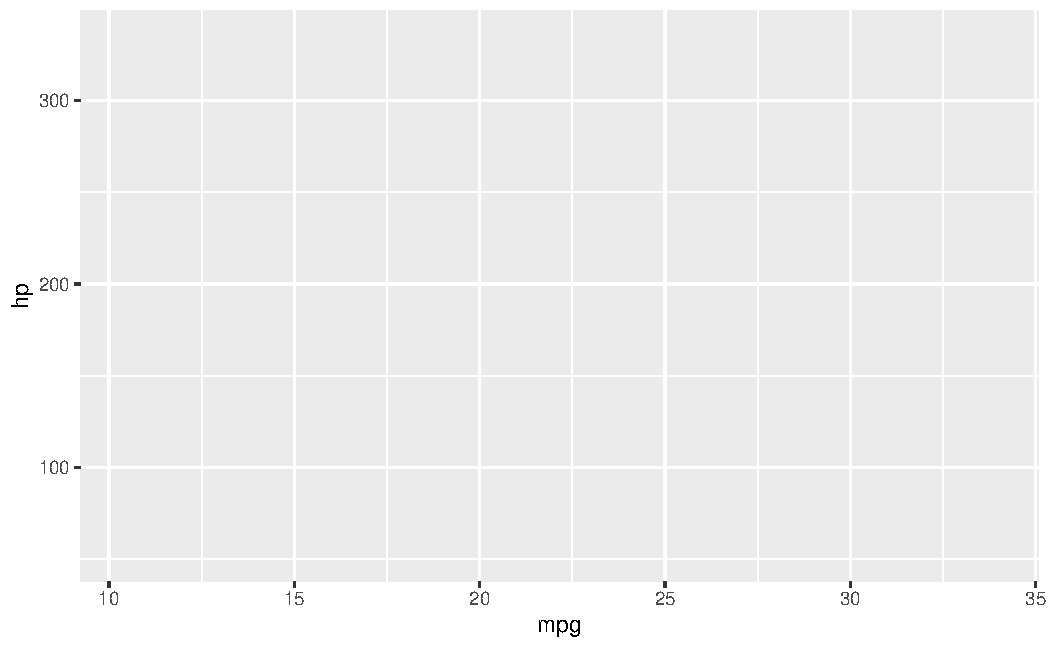
\includegraphics[width=1\linewidth]{mastering-r-through-errors_files/figure-latex/unnamed-chunk-784-1} \end{center}

\subsubsection{Cause 3: Function Not Created Yet}\label{cause-3-function-not-created-yet}

\begin{Shaded}
\begin{Highlighting}[]
\CommentTok{\# Calling before definition}
\NormalTok{result }\OtherTok{\textless{}{-}} \FunctionTok{calculate\_total}\NormalTok{(}\DecValTok{10}\NormalTok{, }\DecValTok{20}\NormalTok{)}

\NormalTok{calculate\_total }\OtherTok{\textless{}{-}} \ControlFlowTok{function}\NormalTok{(a, b) \{}
\NormalTok{  a }\SpecialCharTok{+}\NormalTok{ b}
\NormalTok{\}}
\end{Highlighting}
\end{Shaded}

\subsubsection{Cause 4: Wrong Scope}\label{cause-4-wrong-scope}

\begin{Shaded}
\begin{Highlighting}[]
\CommentTok{\# Function created in different environment}
\NormalTok{\{}
\NormalTok{  local\_func }\OtherTok{\textless{}{-}} \ControlFlowTok{function}\NormalTok{(x) x }\SpecialCharTok{*} \DecValTok{2}
\NormalTok{\}}

\FunctionTok{local\_func}\NormalTok{(}\DecValTok{5}\NormalTok{)  }\CommentTok{\# No longer accessible}
\CommentTok{\#\textgreater{} [1] 10}
\end{Highlighting}
\end{Shaded}

\subsection{Solutions}\label{solutions-72}

✅ \textbf{SOLUTION 1: Check Spelling}

\begin{Shaded}
\begin{Highlighting}[]
\CommentTok{\# Use tab completion in RStudio}
\CommentTok{\# Type first few letters and press Tab}

\CommentTok{\# Check available functions}
\FunctionTok{apropos}\NormalTok{(}\StringTok{"mean"}\NormalTok{)  }\CommentTok{\# Find functions with "mean" in name}
\CommentTok{\#\textgreater{}  [1] ".colMeans"        ".rowMeans"        "calculate\_mean"   "col\_means"       }
\CommentTok{\#\textgreater{}  [5] "colMeans"         "cummean"          "group\_means"      "kmeans"          }
\CommentTok{\#\textgreater{}  [9] "mean"             "mean\_cl\_boot"     "mean\_cl\_normal"   "mean\_cpp"        }
\CommentTok{\#\textgreater{} [13] "mean\_r"           "mean\_sdl"         "mean\_se"          "mean\_val"        }
\CommentTok{\#\textgreater{} [17] "mean.Date"        "mean.default"     "mean.difftime"    "mean.POSIXct"    }
\CommentTok{\#\textgreater{} [21] "mean.POSIXlt"     "mpg\_mean"         "my\_mean"          "my\_mean\_value"   }
\CommentTok{\#\textgreater{} [25] "robust\_mean"      "rollmean"         "rollmean.default" "rollmeanr"       }
\CommentTok{\#\textgreater{} [29] "row\_means\_apply"  "rowMeans"         "verbose\_mean"     "weighted.mean"}

\CommentTok{\# Search help}
\NormalTok{??mean}
\end{Highlighting}
\end{Shaded}

✅ \textbf{SOLUTION 2: Load Required Package}

\begin{Shaded}
\begin{Highlighting}[]
\CommentTok{\# Check if function is in a package}
\FunctionTok{help.search}\NormalTok{(}\StringTok{"ggplot"}\NormalTok{)}

\CommentTok{\# Load package}
\FunctionTok{library}\NormalTok{(ggplot2)}

\CommentTok{\# Or use package::function syntax}
\NormalTok{ggplot2}\SpecialCharTok{::}\FunctionTok{ggplot}\NormalTok{(mtcars, }\FunctionTok{aes}\NormalTok{(}\AttributeTok{x =}\NormalTok{ mpg, }\AttributeTok{y =}\NormalTok{ hp))}
\end{Highlighting}
\end{Shaded}

\begin{center}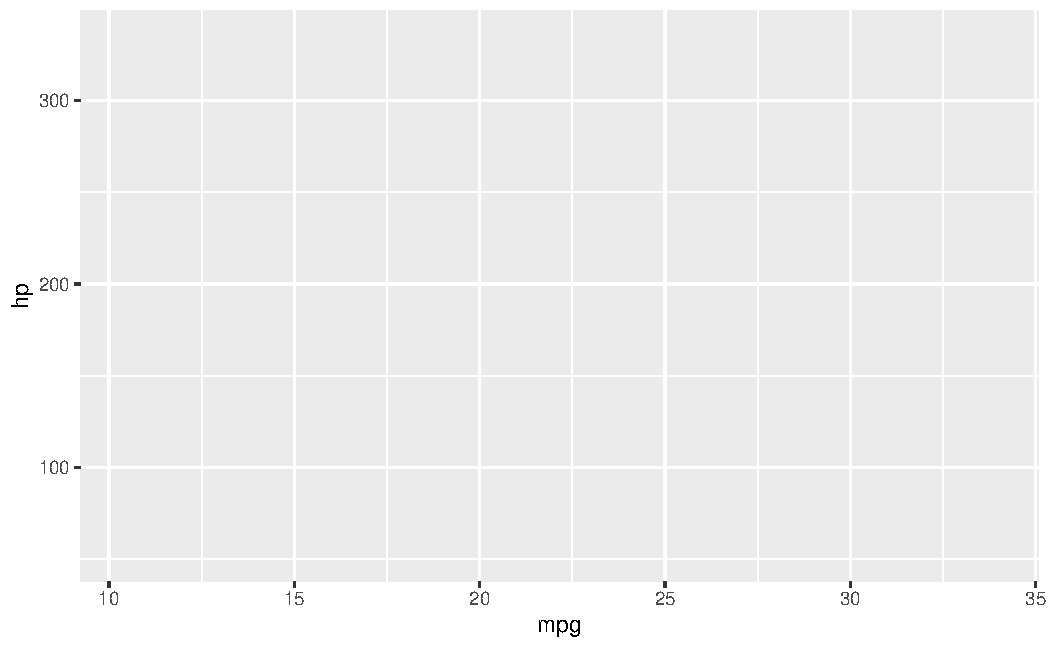
\includegraphics[width=1\linewidth]{mastering-r-through-errors_files/figure-latex/unnamed-chunk-788-1} \end{center}

✅ \textbf{SOLUTION 3: Check Function Exists}

\begin{Shaded}
\begin{Highlighting}[]
\NormalTok{safe\_call }\OtherTok{\textless{}{-}} \ControlFlowTok{function}\NormalTok{(func\_name, ...) \{}
  \ControlFlowTok{if}\NormalTok{ (}\SpecialCharTok{!}\FunctionTok{exists}\NormalTok{(func\_name, }\AttributeTok{mode =} \StringTok{"function"}\NormalTok{)) \{}
    \FunctionTok{stop}\NormalTok{(}\StringTok{"Function \textquotesingle{}"}\NormalTok{, func\_name, }\StringTok{"\textquotesingle{} not found. "}\NormalTok{,}
         \StringTok{"Did you mean: "}\NormalTok{, }\FunctionTok{paste}\NormalTok{(}\FunctionTok{apropos}\NormalTok{(func\_name), }\AttributeTok{collapse =} \StringTok{", "}\NormalTok{))}
\NormalTok{  \}}
  
  \FunctionTok{do.call}\NormalTok{(func\_name, }\FunctionTok{list}\NormalTok{(...))}
\NormalTok{\}}

\CommentTok{\# Test}
\FunctionTok{safe\_call}\NormalTok{(}\StringTok{"mean"}\NormalTok{, }\FunctionTok{c}\NormalTok{(}\DecValTok{1}\NormalTok{, }\DecValTok{2}\NormalTok{, }\DecValTok{3}\NormalTok{))}
\CommentTok{\#\textgreater{} [1] 2}
\end{Highlighting}
\end{Shaded}

\begin{Shaded}
\begin{Highlighting}[]
\FunctionTok{safe\_call}\NormalTok{(}\StringTok{"maen"}\NormalTok{, }\FunctionTok{c}\NormalTok{(}\DecValTok{1}\NormalTok{, }\DecValTok{2}\NormalTok{, }\DecValTok{3}\NormalTok{))  }\CommentTok{\# Helpful error}
\CommentTok{\#\textgreater{} Error in safe\_call("maen", c(1, 2, 3)): Function \textquotesingle{}maen\textquotesingle{} not found. Did you mean:}
\end{Highlighting}
\end{Shaded}

\section{\texorpdfstring{Error \#2: \texttt{argument\ "x"\ is\ missing,\ with\ no\ default}}{Error \#2: argument "x" is missing, with no default}}\label{argument-missing}

{⭐ BEGINNER} {📋 ARGS}

\subsection{The Error}\label{the-error-64}

\begin{Shaded}
\begin{Highlighting}[]
\NormalTok{my\_func }\OtherTok{\textless{}{-}} \ControlFlowTok{function}\NormalTok{(x, y) \{}
\NormalTok{  x }\SpecialCharTok{+}\NormalTok{ y}
\NormalTok{\}}

\FunctionTok{my\_func}\NormalTok{(}\DecValTok{5}\NormalTok{)  }\CommentTok{\# Missing y!}
\CommentTok{\#\textgreater{} Error in my\_func(5): argument "y" is missing, with no default}
\end{Highlighting}
\end{Shaded}

🔴 \textbf{ERROR}

\begin{verbatim}
Error in my_func(5) : argument "y" is missing, with no default
\end{verbatim}

\subsection{What It Means}\label{what-it-means-69}

You're calling a function without providing all required arguments.

\subsection{Understanding Arguments}\label{understanding-arguments}

\begin{Shaded}
\begin{Highlighting}[]
\CommentTok{\# Required arguments (no default)}
\NormalTok{func1 }\OtherTok{\textless{}{-}} \ControlFlowTok{function}\NormalTok{(x, y) \{}
\NormalTok{  x }\SpecialCharTok{+}\NormalTok{ y}
\NormalTok{\}}

\FunctionTok{func1}\NormalTok{(}\DecValTok{5}\NormalTok{, }\DecValTok{10}\NormalTok{)  }\CommentTok{\# Must provide both}
\CommentTok{\#\textgreater{} [1] 15}
\end{Highlighting}
\end{Shaded}

\begin{Shaded}
\begin{Highlighting}[]
\FunctionTok{func1}\NormalTok{(}\DecValTok{5}\NormalTok{)      }\CommentTok{\# Error!}
\CommentTok{\#\textgreater{} Error in func1(5): argument "y" is missing, with no default}
\end{Highlighting}
\end{Shaded}

\begin{Shaded}
\begin{Highlighting}[]
\CommentTok{\# Optional arguments (with default)}
\NormalTok{func2 }\OtherTok{\textless{}{-}} \ControlFlowTok{function}\NormalTok{(x, }\AttributeTok{y =} \DecValTok{10}\NormalTok{) \{}
\NormalTok{  x }\SpecialCharTok{+}\NormalTok{ y}
\NormalTok{\}}

\FunctionTok{func2}\NormalTok{(}\DecValTok{5}\NormalTok{, }\DecValTok{20}\NormalTok{)  }\CommentTok{\# Can override default}
\CommentTok{\#\textgreater{} [1] 25}
\FunctionTok{func2}\NormalTok{(}\DecValTok{5}\NormalTok{)      }\CommentTok{\# Uses default y = 10}
\CommentTok{\#\textgreater{} [1] 15}

\CommentTok{\# All optional}
\NormalTok{func3 }\OtherTok{\textless{}{-}} \ControlFlowTok{function}\NormalTok{(}\AttributeTok{x =} \DecValTok{5}\NormalTok{, }\AttributeTok{y =} \DecValTok{10}\NormalTok{) \{}
\NormalTok{  x }\SpecialCharTok{+}\NormalTok{ y}
\NormalTok{\}}

\FunctionTok{func3}\NormalTok{()       }\CommentTok{\# Uses all defaults}
\CommentTok{\#\textgreater{} [1] 15}
\FunctionTok{func3}\NormalTok{(}\DecValTok{8}\NormalTok{)      }\CommentTok{\# Override x, use default y}
\CommentTok{\#\textgreater{} [1] 18}
\FunctionTok{func3}\NormalTok{(}\DecValTok{8}\NormalTok{, }\DecValTok{12}\NormalTok{)  }\CommentTok{\# Override both}
\CommentTok{\#\textgreater{} [1] 20}
\end{Highlighting}
\end{Shaded}

\subsection{Solutions}\label{solutions-73}

✅ \textbf{SOLUTION 1: Provide All Required Arguments}

\begin{Shaded}
\begin{Highlighting}[]
\NormalTok{my\_func }\OtherTok{\textless{}{-}} \ControlFlowTok{function}\NormalTok{(x, y) \{}
\NormalTok{  x }\SpecialCharTok{+}\NormalTok{ y}
\NormalTok{\}}

\CommentTok{\# Call with all arguments}
\FunctionTok{my\_func}\NormalTok{(}\DecValTok{5}\NormalTok{, }\DecValTok{10}\NormalTok{)}
\CommentTok{\#\textgreater{} [1] 15}

\CommentTok{\# Named arguments (order doesn\textquotesingle{}t matter)}
\FunctionTok{my\_func}\NormalTok{(}\AttributeTok{y =} \DecValTok{10}\NormalTok{, }\AttributeTok{x =} \DecValTok{5}\NormalTok{)}
\CommentTok{\#\textgreater{} [1] 15}
\end{Highlighting}
\end{Shaded}

✅ \textbf{SOLUTION 2: Add Default Values}

\begin{Shaded}
\begin{Highlighting}[]
\CommentTok{\# Make some/all arguments optional}
\NormalTok{my\_func }\OtherTok{\textless{}{-}} \ControlFlowTok{function}\NormalTok{(x, }\AttributeTok{y =} \DecValTok{0}\NormalTok{) \{}
\NormalTok{  x }\SpecialCharTok{+}\NormalTok{ y}
\NormalTok{\}}

\FunctionTok{my\_func}\NormalTok{(}\DecValTok{5}\NormalTok{)     }\CommentTok{\# Works, y defaults to 0}
\CommentTok{\#\textgreater{} [1] 5}
\FunctionTok{my\_func}\NormalTok{(}\DecValTok{5}\NormalTok{, }\DecValTok{10}\NormalTok{) }\CommentTok{\# Can still override}
\CommentTok{\#\textgreater{} [1] 15}

\CommentTok{\# Can use NULL as default}
\NormalTok{my\_func2 }\OtherTok{\textless{}{-}} \ControlFlowTok{function}\NormalTok{(x, }\AttributeTok{y =} \ConstantTok{NULL}\NormalTok{) \{}
  \ControlFlowTok{if}\NormalTok{ (}\FunctionTok{is.null}\NormalTok{(y)) \{}
\NormalTok{    y }\OtherTok{\textless{}{-}}\NormalTok{ x  }\CommentTok{\# Default to same as x}
\NormalTok{  \}}
\NormalTok{  x }\SpecialCharTok{+}\NormalTok{ y}
\NormalTok{\}}

\FunctionTok{my\_func2}\NormalTok{(}\DecValTok{5}\NormalTok{)}
\CommentTok{\#\textgreater{} [1] 10}
\FunctionTok{my\_func2}\NormalTok{(}\DecValTok{5}\NormalTok{, }\DecValTok{3}\NormalTok{)}
\CommentTok{\#\textgreater{} [1] 8}
\end{Highlighting}
\end{Shaded}

✅ \textbf{SOLUTION 3: Check Arguments}

\begin{Shaded}
\begin{Highlighting}[]
\NormalTok{my\_func }\OtherTok{\textless{}{-}} \ControlFlowTok{function}\NormalTok{(x, y) \{}
  \CommentTok{\# Check if arguments provided}
  \ControlFlowTok{if}\NormalTok{ (}\FunctionTok{missing}\NormalTok{(x)) \{}
    \FunctionTok{stop}\NormalTok{(}\StringTok{"Argument \textquotesingle{}x\textquotesingle{} is required"}\NormalTok{)}
\NormalTok{  \}}
  \ControlFlowTok{if}\NormalTok{ (}\FunctionTok{missing}\NormalTok{(y)) \{}
    \FunctionTok{message}\NormalTok{(}\StringTok{"Argument \textquotesingle{}y\textquotesingle{} not provided, using default of 0"}\NormalTok{)}
\NormalTok{    y }\OtherTok{\textless{}{-}} \DecValTok{0}
\NormalTok{  \}}
  
\NormalTok{  x }\SpecialCharTok{+}\NormalTok{ y}
\NormalTok{\}}

\FunctionTok{my\_func}\NormalTok{(}\DecValTok{5}\NormalTok{)    }\CommentTok{\# Warning but works}
\CommentTok{\#\textgreater{} Argument \textquotesingle{}y\textquotesingle{} not provided, using default of 0}
\CommentTok{\#\textgreater{} [1] 5}
\FunctionTok{my\_func}\NormalTok{(}\DecValTok{5}\NormalTok{, }\DecValTok{3}\NormalTok{)}
\CommentTok{\#\textgreater{} [1] 8}
\end{Highlighting}
\end{Shaded}

\begin{Shaded}
\begin{Highlighting}[]
\FunctionTok{my\_func}\NormalTok{()     }\CommentTok{\# Clear error about x}
\CommentTok{\#\textgreater{} Error in my\_func(): Argument \textquotesingle{}x\textquotesingle{} is required}
\end{Highlighting}
\end{Shaded}

\section{\texorpdfstring{Error \#3: \texttt{unused\ argument}}{Error \#3: unused argument}}\label{unused-argument}

{⭐ BEGINNER} {📋 ARGS}

\subsection{The Error}\label{the-error-65}

\begin{Shaded}
\begin{Highlighting}[]
\NormalTok{my\_func }\OtherTok{\textless{}{-}} \ControlFlowTok{function}\NormalTok{(x, y) \{}
\NormalTok{  x }\SpecialCharTok{+}\NormalTok{ y}
\NormalTok{\}}

\FunctionTok{my\_func}\NormalTok{(}\DecValTok{5}\NormalTok{, }\DecValTok{10}\NormalTok{, }\DecValTok{15}\NormalTok{)  }\CommentTok{\# Too many arguments!}
\CommentTok{\#\textgreater{} Error in my\_func(5, 10, 15): unused argument (15)}
\end{Highlighting}
\end{Shaded}

🔴 \textbf{ERROR}

\begin{verbatim}
Error in my_func(5, 10, 15) : unused argument (15)
\end{verbatim}

\subsection{What It Means}\label{what-it-means-70}

You're passing more arguments than the function accepts.

\subsection{Common Causes}\label{common-causes-45}

\subsubsection{Cause 1: Extra Arguments}\label{cause-1-extra-arguments}

\begin{Shaded}
\begin{Highlighting}[]
\FunctionTok{mean}\NormalTok{(}\FunctionTok{c}\NormalTok{(}\DecValTok{1}\NormalTok{, }\DecValTok{2}\NormalTok{, }\ConstantTok{NA}\NormalTok{), }\AttributeTok{na.rm =} \ConstantTok{TRUE}\NormalTok{, }\AttributeTok{extra =} \StringTok{"oops"}\NormalTok{)}
\CommentTok{\#\textgreater{} [1] 1.5}
\end{Highlighting}
\end{Shaded}

\subsubsection{Cause 2: Wrong Argument Name}\label{cause-2-wrong-argument-name}

\begin{Shaded}
\begin{Highlighting}[]
\FunctionTok{mean}\NormalTok{(}\FunctionTok{c}\NormalTok{(}\DecValTok{1}\NormalTok{, }\DecValTok{2}\NormalTok{, }\ConstantTok{NA}\NormalTok{), }\AttributeTok{remove\_na =} \ConstantTok{TRUE}\NormalTok{)  }\CommentTok{\# It\textquotesingle{}s na.rm not remove\_na}
\CommentTok{\#\textgreater{} [1] NA}
\end{Highlighting}
\end{Shaded}

\subsubsection{Cause 3: Positional Confusion}\label{cause-3-positional-confusion}

\begin{Shaded}
\begin{Highlighting}[]
\CommentTok{\# substr expects (x, start, stop)}
\FunctionTok{substr}\NormalTok{(}\StringTok{"hello"}\NormalTok{, }\DecValTok{1}\NormalTok{, }\DecValTok{3}\NormalTok{, }\StringTok{"extra"}\NormalTok{)}
\CommentTok{\#\textgreater{} Error in substr("hello", 1, 3, "extra"): unused argument ("extra")}
\end{Highlighting}
\end{Shaded}

\subsection{Solutions}\label{solutions-74}

✅ \textbf{SOLUTION 1: Remove Extra Arguments}

\begin{Shaded}
\begin{Highlighting}[]
\CommentTok{\# Check function signature}
\FunctionTok{args}\NormalTok{(mean)}
\CommentTok{\#\textgreater{} function (x, ...) }
\CommentTok{\#\textgreater{} NULL}

\CommentTok{\# Provide correct arguments only}
\FunctionTok{mean}\NormalTok{(}\FunctionTok{c}\NormalTok{(}\DecValTok{1}\NormalTok{, }\DecValTok{2}\NormalTok{, }\ConstantTok{NA}\NormalTok{), }\AttributeTok{na.rm =} \ConstantTok{TRUE}\NormalTok{)}
\CommentTok{\#\textgreater{} [1] 1.5}
\end{Highlighting}
\end{Shaded}

✅ \textbf{SOLUTION 2: Use \ldots{} to Accept Extra Arguments}

\begin{Shaded}
\begin{Highlighting}[]
\CommentTok{\# Allow any number of additional arguments}
\NormalTok{my\_func }\OtherTok{\textless{}{-}} \ControlFlowTok{function}\NormalTok{(x, y, ...) \{}
\NormalTok{  result }\OtherTok{\textless{}{-}}\NormalTok{ x }\SpecialCharTok{+}\NormalTok{ y}
  
  \CommentTok{\# Can pass ... to other functions}
\NormalTok{  extra\_args }\OtherTok{\textless{}{-}} \FunctionTok{list}\NormalTok{(...)}
  \ControlFlowTok{if}\NormalTok{ (}\FunctionTok{length}\NormalTok{(extra\_args) }\SpecialCharTok{\textgreater{}} \DecValTok{0}\NormalTok{) \{}
    \FunctionTok{message}\NormalTok{(}\StringTok{"Ignoring extra arguments: "}\NormalTok{, }
            \FunctionTok{paste}\NormalTok{(}\FunctionTok{names}\NormalTok{(extra\_args), }\AttributeTok{collapse =} \StringTok{", "}\NormalTok{))}
\NormalTok{  \}}
  
\NormalTok{  result}
\NormalTok{\}}

\FunctionTok{my\_func}\NormalTok{(}\DecValTok{5}\NormalTok{, }\DecValTok{10}\NormalTok{)              }\CommentTok{\# Works}
\CommentTok{\#\textgreater{} [1] 15}
\FunctionTok{my\_func}\NormalTok{(}\DecValTok{5}\NormalTok{, }\DecValTok{10}\NormalTok{, }\AttributeTok{z =} \DecValTok{15}\NormalTok{)      }\CommentTok{\# Works, ignores z}
\CommentTok{\#\textgreater{} Ignoring extra arguments: z}
\CommentTok{\#\textgreater{} [1] 15}
\FunctionTok{my\_func}\NormalTok{(}\DecValTok{5}\NormalTok{, }\DecValTok{10}\NormalTok{, }\DecValTok{15}\NormalTok{, }\DecValTok{20}\NormalTok{)      }\CommentTok{\# Works, ignores unnamed extras}
\CommentTok{\#\textgreater{} Ignoring extra arguments:}
\CommentTok{\#\textgreater{} [1] 15}
\end{Highlighting}
\end{Shaded}

✅ \textbf{SOLUTION 3: Validate Arguments}

\begin{Shaded}
\begin{Highlighting}[]
\NormalTok{my\_func }\OtherTok{\textless{}{-}} \ControlFlowTok{function}\NormalTok{(x, y) \{}
  \CommentTok{\# Capture call}
\NormalTok{  call }\OtherTok{\textless{}{-}} \FunctionTok{match.call}\NormalTok{()}
  
  \CommentTok{\# Check for unexpected arguments}
\NormalTok{  valid\_args }\OtherTok{\textless{}{-}} \FunctionTok{c}\NormalTok{(}\StringTok{"x"}\NormalTok{, }\StringTok{"y"}\NormalTok{)}
\NormalTok{  provided\_args }\OtherTok{\textless{}{-}} \FunctionTok{names}\NormalTok{(call)[}\SpecialCharTok{{-}}\DecValTok{1}\NormalTok{]  }\CommentTok{\# Remove function name}
  
\NormalTok{  invalid }\OtherTok{\textless{}{-}} \FunctionTok{setdiff}\NormalTok{(provided\_args, valid\_args)}
  \ControlFlowTok{if}\NormalTok{ (}\FunctionTok{length}\NormalTok{(invalid) }\SpecialCharTok{\textgreater{}} \DecValTok{0}\NormalTok{) \{}
    \FunctionTok{stop}\NormalTok{(}\StringTok{"Unexpected arguments: "}\NormalTok{, }\FunctionTok{paste}\NormalTok{(invalid, }\AttributeTok{collapse =} \StringTok{", "}\NormalTok{),}
         \StringTok{"}\SpecialCharTok{\textbackslash{}n}\StringTok{Valid arguments are: "}\NormalTok{, }\FunctionTok{paste}\NormalTok{(valid\_args, }\AttributeTok{collapse =} \StringTok{", "}\NormalTok{))}
\NormalTok{  \}}
  
\NormalTok{  x }\SpecialCharTok{+}\NormalTok{ y}
\NormalTok{\}}

\FunctionTok{my\_func}\NormalTok{(}\DecValTok{5}\NormalTok{, }\DecValTok{10}\NormalTok{)}
\CommentTok{\#\textgreater{} [1] 15}
\end{Highlighting}
\end{Shaded}

\begin{Shaded}
\begin{Highlighting}[]
\FunctionTok{my\_func}\NormalTok{(}\DecValTok{5}\NormalTok{, }\DecValTok{10}\NormalTok{, }\AttributeTok{z =} \DecValTok{15}\NormalTok{)  }\CommentTok{\# Helpful error}
\CommentTok{\#\textgreater{} Error in my\_func(5, 10, z = 15): unused argument (z = 15)}
\end{Highlighting}
\end{Shaded}

\section{Return Values}\label{return-values}

💡 \textbf{Key Insight: Return Values}

\begin{Shaded}
\begin{Highlighting}[]
\CommentTok{\# Implicit return (last expression)}
\NormalTok{func1 }\OtherTok{\textless{}{-}} \ControlFlowTok{function}\NormalTok{(x) \{}
\NormalTok{  x }\SpecialCharTok{*} \DecValTok{2}
\NormalTok{\}}
\FunctionTok{func1}\NormalTok{(}\DecValTok{5}\NormalTok{)  }\CommentTok{\# Returns 10}
\CommentTok{\#\textgreater{} [1] 10}

\CommentTok{\# Explicit return}
\NormalTok{func2 }\OtherTok{\textless{}{-}} \ControlFlowTok{function}\NormalTok{(x) \{}
  \FunctionTok{return}\NormalTok{(x }\SpecialCharTok{*} \DecValTok{2}\NormalTok{)}
\NormalTok{\}}
\FunctionTok{func2}\NormalTok{(}\DecValTok{5}\NormalTok{)  }\CommentTok{\# Returns 10}
\CommentTok{\#\textgreater{} [1] 10}

\CommentTok{\# Early return}
\NormalTok{func3 }\OtherTok{\textless{}{-}} \ControlFlowTok{function}\NormalTok{(x) \{}
  \ControlFlowTok{if}\NormalTok{ (x }\SpecialCharTok{\textless{}} \DecValTok{0}\NormalTok{) \{}
    \FunctionTok{return}\NormalTok{(}\DecValTok{0}\NormalTok{)  }\CommentTok{\# Exit early}
\NormalTok{  \}}
\NormalTok{  x }\SpecialCharTok{*} \DecValTok{2}
\NormalTok{\}}
\FunctionTok{func3}\NormalTok{(}\SpecialCharTok{{-}}\DecValTok{5}\NormalTok{)  }\CommentTok{\# Returns 0}
\CommentTok{\#\textgreater{} [1] 0}
\FunctionTok{func3}\NormalTok{(}\DecValTok{5}\NormalTok{)   }\CommentTok{\# Returns 10}
\CommentTok{\#\textgreater{} [1] 10}

\CommentTok{\# No return (returns NULL)}
\NormalTok{func4 }\OtherTok{\textless{}{-}} \ControlFlowTok{function}\NormalTok{(x) \{}
\NormalTok{  result }\OtherTok{\textless{}{-}}\NormalTok{ x }\SpecialCharTok{*} \DecValTok{2}
  \CommentTok{\# Forgot to return or print result}
\NormalTok{\}}
\FunctionTok{func4}\NormalTok{(}\DecValTok{5}\NormalTok{)  }\CommentTok{\# Returns NULL invisibly}

\CommentTok{\# Multiple values (use list)}
\NormalTok{func5 }\OtherTok{\textless{}{-}} \ControlFlowTok{function}\NormalTok{(x) \{}
  \FunctionTok{list}\NormalTok{(}
    \AttributeTok{original =}\NormalTok{ x,}
    \AttributeTok{doubled =}\NormalTok{ x }\SpecialCharTok{*} \DecValTok{2}\NormalTok{,}
    \AttributeTok{squared =}\NormalTok{ x}\SpecialCharTok{\^{}}\DecValTok{2}
\NormalTok{  )}
\NormalTok{\}}
\FunctionTok{func5}\NormalTok{(}\DecValTok{5}\NormalTok{)}
\CommentTok{\#\textgreater{} $original}
\CommentTok{\#\textgreater{} [1] 5}
\CommentTok{\#\textgreater{} }
\CommentTok{\#\textgreater{} $doubled}
\CommentTok{\#\textgreater{} [1] 10}
\CommentTok{\#\textgreater{} }
\CommentTok{\#\textgreater{} $squared}
\CommentTok{\#\textgreater{} [1] 25}

\CommentTok{\# Return NULL explicitly}
\NormalTok{func6 }\OtherTok{\textless{}{-}} \ControlFlowTok{function}\NormalTok{(x) \{}
  \ControlFlowTok{if}\NormalTok{ (x }\SpecialCharTok{\textless{}} \DecValTok{0}\NormalTok{) \{}
    \FunctionTok{return}\NormalTok{(}\ConstantTok{NULL}\NormalTok{)}
\NormalTok{  \}}
\NormalTok{  x }\SpecialCharTok{*} \DecValTok{2}
\NormalTok{\}}
\FunctionTok{func6}\NormalTok{(}\SpecialCharTok{{-}}\DecValTok{5}\NormalTok{)  }\CommentTok{\# NULL}
\CommentTok{\#\textgreater{} NULL}
\FunctionTok{func6}\NormalTok{(}\DecValTok{5}\NormalTok{)   }\CommentTok{\# 10}
\CommentTok{\#\textgreater{} [1] 10}
\end{Highlighting}
\end{Shaded}

\textbf{Best practices:}
- Last expression is returned automatically
- Use \texttt{return()} for early exits
- Use \texttt{invisible()} for functions with side effects
- Return lists for multiple values

\section{\texorpdfstring{Error \#4: \texttt{object\ of\ type\ \textquotesingle{}closure\textquotesingle{}\ is\ not\ subsettable}}{Error \#4: object of type \textquotesingle closure\textquotesingle{} is not subsettable}}\label{closure-not-subsettable}

{⭐⭐ INTERMEDIATE} {🔢 TYPE}

\subsection{The Error}\label{the-error-66}

\begin{Shaded}
\begin{Highlighting}[]
\NormalTok{my\_func }\OtherTok{\textless{}{-}} \ControlFlowTok{function}\NormalTok{(x) x }\SpecialCharTok{*} \DecValTok{2}

\CommentTok{\# Try to subset a function}
\NormalTok{my\_func[}\DecValTok{1}\NormalTok{]}
\CommentTok{\#\textgreater{} Error in my\_func[1]: object of type \textquotesingle{}closure\textquotesingle{} is not subsettable}
\end{Highlighting}
\end{Shaded}

🔴 \textbf{ERROR}

\begin{verbatim}
Error in my_func[1] : object of type 'closure' is not subsettable
\end{verbatim}

\subsection{What It Means}\label{what-it-means-71}

You're trying to subset a function as if it were a vector or list. ``Closure'' is R's internal name for functions.

\subsection{Common Causes}\label{common-causes-46}

\subsubsection{Cause 1: Name Collision}\label{cause-1-name-collision}

\begin{Shaded}
\begin{Highlighting}[]
\CommentTok{\# Accidentally named data same as function}
\NormalTok{mean }\OtherTok{\textless{}{-}} \ControlFlowTok{function}\NormalTok{(x) }\FunctionTok{sum}\NormalTok{(x) }\SpecialCharTok{/} \FunctionTok{length}\NormalTok{(x)}

\CommentTok{\# Later, try to use mean as data}
\NormalTok{mean[}\DecValTok{1}\NormalTok{]  }\CommentTok{\# Error! mean is now a function}
\CommentTok{\#\textgreater{} Error in mean[1]: object of type \textquotesingle{}closure\textquotesingle{} is not subsettable}
\end{Highlighting}
\end{Shaded}

\subsubsection{Cause 2: Forgot to Call Function}\label{cause-2-forgot-to-call-function}

\begin{Shaded}
\begin{Highlighting}[]
\NormalTok{data }\OtherTok{\textless{}{-}} \FunctionTok{c}\NormalTok{(}\DecValTok{1}\NormalTok{, }\DecValTok{2}\NormalTok{, }\DecValTok{3}\NormalTok{, }\DecValTok{4}\NormalTok{, }\DecValTok{5}\NormalTok{)}

\CommentTok{\# Forgot parentheses}
\NormalTok{result }\OtherTok{\textless{}{-}}\NormalTok{ mean  }\CommentTok{\# Assigns the function, not result}
\NormalTok{result[}\DecValTok{1}\NormalTok{]       }\CommentTok{\# Error!}
\CommentTok{\#\textgreater{} Error in result[1]: object of type \textquotesingle{}closure\textquotesingle{} is not subsettable}
\end{Highlighting}
\end{Shaded}

\subsubsection{Cause 3: Wrong Object}\label{cause-3-wrong-object}

\begin{Shaded}
\begin{Highlighting}[]
\NormalTok{my\_list }\OtherTok{\textless{}{-}} \FunctionTok{list}\NormalTok{(}\AttributeTok{a =} \DecValTok{1}\NormalTok{, }\AttributeTok{b =} \DecValTok{2}\NormalTok{)}
\NormalTok{my\_func }\OtherTok{\textless{}{-}} \ControlFlowTok{function}\NormalTok{(x) x }\SpecialCharTok{*} \DecValTok{2}

\CommentTok{\# Accidentally use function instead of list}
\NormalTok{my\_func}\SpecialCharTok{$}\NormalTok{a}
\CommentTok{\#\textgreater{} Error in my\_func$a: object of type \textquotesingle{}closure\textquotesingle{} is not subsettable}
\end{Highlighting}
\end{Shaded}

\subsection{Solutions}\label{solutions-75}

✅ \textbf{SOLUTION 1: Check Object Type}

\begin{Shaded}
\begin{Highlighting}[]
\NormalTok{my\_func }\OtherTok{\textless{}{-}} \ControlFlowTok{function}\NormalTok{(x) x }\SpecialCharTok{*} \DecValTok{2}

\CommentTok{\# Check what it is}
\FunctionTok{is.function}\NormalTok{(my\_func)}
\CommentTok{\#\textgreater{} [1] TRUE}
\FunctionTok{class}\NormalTok{(my\_func)}
\CommentTok{\#\textgreater{} [1] "function"}

\CommentTok{\# If you need to subset, make sure you\textquotesingle{}re using the right object}
\end{Highlighting}
\end{Shaded}

✅ \textbf{SOLUTION 2: Call Function Properly}

\begin{Shaded}
\begin{Highlighting}[]
\CommentTok{\# Call the function}
\NormalTok{result }\OtherTok{\textless{}{-}} \FunctionTok{mean}\NormalTok{(}\FunctionTok{c}\NormalTok{(}\DecValTok{1}\NormalTok{, }\DecValTok{2}\NormalTok{, }\DecValTok{3}\NormalTok{, }\DecValTok{4}\NormalTok{, }\DecValTok{5}\NormalTok{))}
\NormalTok{result}
\CommentTok{\#\textgreater{} [1] 3}

\CommentTok{\# Now can use result}
\NormalTok{result}
\CommentTok{\#\textgreater{} [1] 3}
\end{Highlighting}
\end{Shaded}

✅ \textbf{SOLUTION 3: Avoid Name Collisions}

\begin{Shaded}
\begin{Highlighting}[]
\CommentTok{\# Don\textquotesingle{}t overwrite common function names}
\CommentTok{\# Bad}
\CommentTok{\# mean \textless{}{-} my\_data}

\CommentTok{\# Good}
\NormalTok{my\_mean\_value }\OtherTok{\textless{}{-}} \FunctionTok{mean}\NormalTok{(my\_data)}

\CommentTok{\# If you accidentally overwrote}
\NormalTok{mean }\OtherTok{\textless{}{-}} \ControlFlowTok{function}\NormalTok{(x) }\FunctionTok{sum}\NormalTok{(x) }\SpecialCharTok{/} \FunctionTok{length}\NormalTok{(x)}

\CommentTok{\# Restore}
\FunctionTok{rm}\NormalTok{(mean)  }\CommentTok{\# Remove your version}
\FunctionTok{mean}\NormalTok{(}\FunctionTok{c}\NormalTok{(}\DecValTok{1}\NormalTok{, }\DecValTok{2}\NormalTok{, }\DecValTok{3}\NormalTok{))  }\CommentTok{\# Uses base::mean again}
\CommentTok{\#\textgreater{} [1] 2}
\end{Highlighting}
\end{Shaded}

\section{Function Arguments: \ldots{} (Dots)}\label{function-arguments-dots}

💡 \textbf{Key Insight: The \ldots{} Argument}

\begin{Shaded}
\begin{Highlighting}[]
\CommentTok{\# ... captures any additional arguments}
\NormalTok{my\_plot }\OtherTok{\textless{}{-}} \ControlFlowTok{function}\NormalTok{(x, y, ...) \{}
  \FunctionTok{plot}\NormalTok{(x, y, ...)  }\CommentTok{\# Pass ... to another function}
\NormalTok{\}}

\CommentTok{\# Can pass any plot arguments}
\FunctionTok{my\_plot}\NormalTok{(}\DecValTok{1}\SpecialCharTok{:}\DecValTok{10}\NormalTok{, }\DecValTok{1}\SpecialCharTok{:}\DecValTok{10}\NormalTok{, }\AttributeTok{col =} \StringTok{"red"}\NormalTok{, }\AttributeTok{pch =} \DecValTok{16}\NormalTok{, }\AttributeTok{main =} \StringTok{"Test"}\NormalTok{)}

\CommentTok{\# Access ... contents}
\NormalTok{my\_func }\OtherTok{\textless{}{-}} \ControlFlowTok{function}\NormalTok{(...) \{}
\NormalTok{  args }\OtherTok{\textless{}{-}} \FunctionTok{list}\NormalTok{(...)}
  \FunctionTok{cat}\NormalTok{(}\StringTok{"Received"}\NormalTok{, }\FunctionTok{length}\NormalTok{(args), }\StringTok{"arguments}\SpecialCharTok{\textbackslash{}n}\StringTok{"}\NormalTok{)}
\NormalTok{  args}
\NormalTok{\}}

\FunctionTok{my\_func}\NormalTok{(}\AttributeTok{a =} \DecValTok{1}\NormalTok{, }\AttributeTok{b =} \DecValTok{2}\NormalTok{, }\AttributeTok{c =} \DecValTok{3}\NormalTok{)}
\CommentTok{\#\textgreater{} Received 3 arguments}
\CommentTok{\#\textgreater{} $a}
\CommentTok{\#\textgreater{} [1] 1}
\CommentTok{\#\textgreater{} }
\CommentTok{\#\textgreater{} $b}
\CommentTok{\#\textgreater{} [1] 2}
\CommentTok{\#\textgreater{} }
\CommentTok{\#\textgreater{} $c}
\CommentTok{\#\textgreater{} [1] 3}

\CommentTok{\# Extract specific arguments from ...}
\NormalTok{my\_func2 }\OtherTok{\textless{}{-}} \ControlFlowTok{function}\NormalTok{(x, ...) \{}
\NormalTok{  dots }\OtherTok{\textless{}{-}} \FunctionTok{list}\NormalTok{(...)}
  
  \CommentTok{\# Get specific argument}
  \ControlFlowTok{if}\NormalTok{ (}\StringTok{"multiplier"} \SpecialCharTok{\%in\%} \FunctionTok{names}\NormalTok{(dots)) \{}
\NormalTok{    mult }\OtherTok{\textless{}{-}}\NormalTok{ dots}\SpecialCharTok{$}\NormalTok{multiplier}
\NormalTok{  \} }\ControlFlowTok{else}\NormalTok{ \{}
\NormalTok{    mult }\OtherTok{\textless{}{-}} \DecValTok{1}
\NormalTok{  \}}
  
\NormalTok{  x }\SpecialCharTok{*}\NormalTok{ mult}
\NormalTok{\}}

\FunctionTok{my\_func2}\NormalTok{(}\DecValTok{5}\NormalTok{)}
\CommentTok{\#\textgreater{} [1] 5}
\FunctionTok{my\_func2}\NormalTok{(}\DecValTok{5}\NormalTok{, }\AttributeTok{multiplier =} \DecValTok{3}\NormalTok{)}
\CommentTok{\#\textgreater{} [1] 15}

\CommentTok{\# Common use: wrapper functions}
\NormalTok{my\_mean }\OtherTok{\textless{}{-}} \ControlFlowTok{function}\NormalTok{(..., }\AttributeTok{na.rm =} \ConstantTok{FALSE}\NormalTok{) \{}
  \CommentTok{\# Add custom behavior}
  \FunctionTok{message}\NormalTok{(}\StringTok{"Calculating mean..."}\NormalTok{)}
  
  \CommentTok{\# Pass to base function}
  \FunctionTok{mean}\NormalTok{(..., }\AttributeTok{na.rm =}\NormalTok{ na.rm)}
\NormalTok{\}}

\FunctionTok{my\_mean}\NormalTok{(}\FunctionTok{c}\NormalTok{(}\DecValTok{1}\NormalTok{, }\DecValTok{2}\NormalTok{, }\ConstantTok{NA}\NormalTok{, }\DecValTok{4}\NormalTok{), }\AttributeTok{na.rm =} \ConstantTok{TRUE}\NormalTok{)}
\CommentTok{\#\textgreater{} Calculating mean...}
\CommentTok{\#\textgreater{} [1] 2.333333}
\end{Highlighting}
\end{Shaded}

\begin{center}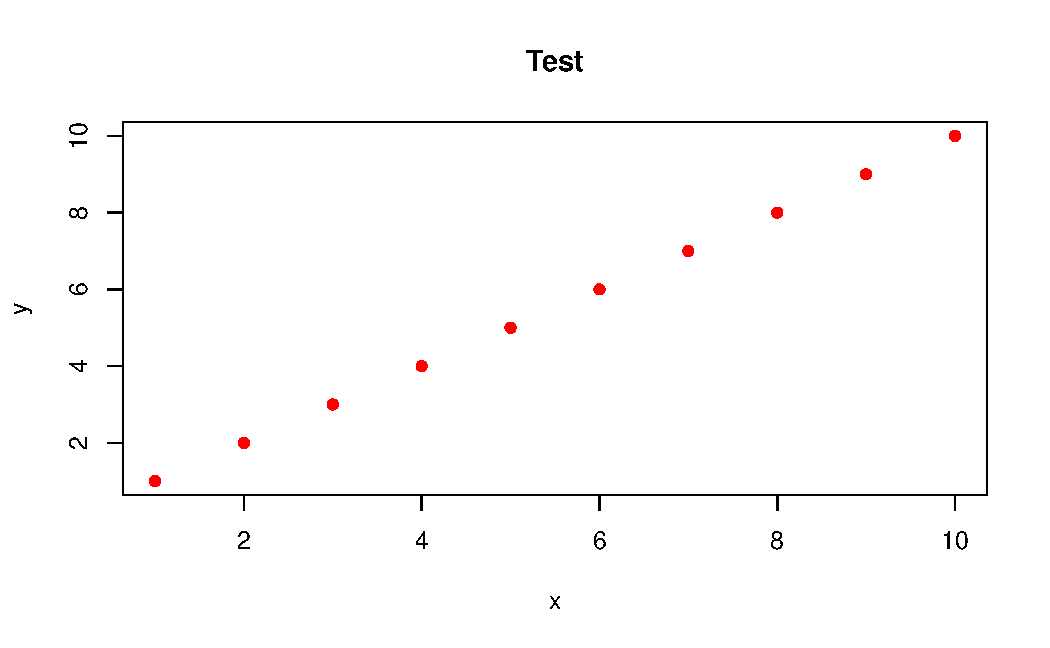
\includegraphics[width=1\linewidth]{mastering-r-through-errors_files/figure-latex/unnamed-chunk-815-1} \end{center}

\textbf{When to use \ldots:}
- Wrapper functions (pass args to another function)
- Flexible functions (accept varying arguments)
- Methods (S3/S4 generics often use \ldots)

\textbf{Caution:}
- Arguments after \ldots{} must be named explicitly
- Easy to make typos that go unnoticed

\section{Argument Matching}\label{argument-matching}

💡 \textbf{Key Insight: How R Matches Arguments}

\begin{Shaded}
\begin{Highlighting}[]
\NormalTok{my\_func }\OtherTok{\textless{}{-}} \ControlFlowTok{function}\NormalTok{(first, second, third) \{}
  \FunctionTok{cat}\NormalTok{(}\StringTok{"first:"}\NormalTok{, first, }\StringTok{"}\SpecialCharTok{\textbackslash{}n}\StringTok{"}\NormalTok{)}
  \FunctionTok{cat}\NormalTok{(}\StringTok{"second:"}\NormalTok{, second, }\StringTok{"}\SpecialCharTok{\textbackslash{}n}\StringTok{"}\NormalTok{)}
  \FunctionTok{cat}\NormalTok{(}\StringTok{"third:"}\NormalTok{, third, }\StringTok{"}\SpecialCharTok{\textbackslash{}n}\StringTok{"}\NormalTok{)}
\NormalTok{\}}

\CommentTok{\# 1. Exact name match}
\FunctionTok{my\_func}\NormalTok{(}\AttributeTok{first =} \DecValTok{1}\NormalTok{, }\AttributeTok{second =} \DecValTok{2}\NormalTok{, }\AttributeTok{third =} \DecValTok{3}\NormalTok{)}
\CommentTok{\#\textgreater{} first: 1 }
\CommentTok{\#\textgreater{} second: 2 }
\CommentTok{\#\textgreater{} third: 3}

\CommentTok{\# 2. Partial name match (not recommended!)}
\FunctionTok{my\_func}\NormalTok{(}\AttributeTok{f =} \DecValTok{1}\NormalTok{, }\AttributeTok{s =} \DecValTok{2}\NormalTok{, }\AttributeTok{t =} \DecValTok{3}\NormalTok{)}
\CommentTok{\#\textgreater{} Warning in my\_func(f = 1, s = 2, t = 3): partial argument match of \textquotesingle{}f\textquotesingle{} to}
\CommentTok{\#\textgreater{} \textquotesingle{}first\textquotesingle{}}
\CommentTok{\#\textgreater{} Warning in my\_func(f = 1, s = 2, t = 3): partial argument match of \textquotesingle{}s\textquotesingle{} to}
\CommentTok{\#\textgreater{} \textquotesingle{}second\textquotesingle{}}
\CommentTok{\#\textgreater{} Warning in my\_func(f = 1, s = 2, t = 3): partial argument match of \textquotesingle{}t\textquotesingle{} to}
\CommentTok{\#\textgreater{} \textquotesingle{}third\textquotesingle{}}
\CommentTok{\#\textgreater{} first: 1 }
\CommentTok{\#\textgreater{} second: 2 }
\CommentTok{\#\textgreater{} third: 3}

\CommentTok{\# 3. Positional match}
\FunctionTok{my\_func}\NormalTok{(}\DecValTok{1}\NormalTok{, }\DecValTok{2}\NormalTok{, }\DecValTok{3}\NormalTok{)}
\CommentTok{\#\textgreater{} first: 1 }
\CommentTok{\#\textgreater{} second: 2 }
\CommentTok{\#\textgreater{} third: 3}

\CommentTok{\# 4. Mixed (named don\textquotesingle{}t need to be in order)}
\FunctionTok{my\_func}\NormalTok{(}\AttributeTok{third =} \DecValTok{3}\NormalTok{, }\AttributeTok{first =} \DecValTok{1}\NormalTok{, }\AttributeTok{second =} \DecValTok{2}\NormalTok{)}
\CommentTok{\#\textgreater{} first: 1 }
\CommentTok{\#\textgreater{} second: 2 }
\CommentTok{\#\textgreater{} third: 3}
\FunctionTok{my\_func}\NormalTok{(}\DecValTok{1}\NormalTok{, }\AttributeTok{third =} \DecValTok{3}\NormalTok{, }\AttributeTok{second =} \DecValTok{2}\NormalTok{)}
\CommentTok{\#\textgreater{} first: 1 }
\CommentTok{\#\textgreater{} second: 2 }
\CommentTok{\#\textgreater{} third: 3}

\CommentTok{\# Order of matching:}
\CommentTok{\# 1. Exact name matches}
\CommentTok{\# 2. Partial name matches  }
\CommentTok{\# 3. Positional matches}
\end{Highlighting}
\end{Shaded}

\textbf{Best practices:}
- Use exact names for clarity
- Avoid partial matching (can cause confusion)
- Use names for all arguments after the first few
- Named arguments can be in any order

\section{Common Function Patterns}\label{common-function-patterns}

🎯 \textbf{Best Practice: Function Patterns}

\begin{Shaded}
\begin{Highlighting}[]
\CommentTok{\# 1. Validate inputs}
\NormalTok{safe\_divide }\OtherTok{\textless{}{-}} \ControlFlowTok{function}\NormalTok{(x, y) \{}
  \CommentTok{\# Check types}
  \ControlFlowTok{if}\NormalTok{ (}\SpecialCharTok{!}\FunctionTok{is.numeric}\NormalTok{(x) }\SpecialCharTok{||} \SpecialCharTok{!}\FunctionTok{is.numeric}\NormalTok{(y)) \{}
    \FunctionTok{stop}\NormalTok{(}\StringTok{"Both x and y must be numeric"}\NormalTok{)}
\NormalTok{  \}}
  
  \CommentTok{\# Check values}
  \ControlFlowTok{if}\NormalTok{ (}\FunctionTok{any}\NormalTok{(y }\SpecialCharTok{==} \DecValTok{0}\NormalTok{)) \{}
    \FunctionTok{stop}\NormalTok{(}\StringTok{"Cannot divide by zero"}\NormalTok{)}
\NormalTok{  \}}
  
\NormalTok{  x }\SpecialCharTok{/}\NormalTok{ y}
\NormalTok{\}}

\FunctionTok{safe\_divide}\NormalTok{(}\DecValTok{10}\NormalTok{, }\DecValTok{2}\NormalTok{)}
\CommentTok{\#\textgreater{} [1] 5}
\end{Highlighting}
\end{Shaded}

\begin{Shaded}
\begin{Highlighting}[]
\FunctionTok{safe\_divide}\NormalTok{(}\DecValTok{10}\NormalTok{, }\DecValTok{0}\NormalTok{)}
\CommentTok{\#\textgreater{} Error in safe\_divide(10, 0): Cannot divide by zero}
\end{Highlighting}
\end{Shaded}

\begin{Shaded}
\begin{Highlighting}[]
\CommentTok{\# 2. Provide informative messages}
\NormalTok{verbose\_mean }\OtherTok{\textless{}{-}} \ControlFlowTok{function}\NormalTok{(x, }\AttributeTok{na.rm =} \ConstantTok{FALSE}\NormalTok{, }\AttributeTok{verbose =} \ConstantTok{TRUE}\NormalTok{) \{}
  \ControlFlowTok{if}\NormalTok{ (verbose) \{}
    \FunctionTok{message}\NormalTok{(}\StringTok{"Calculating mean of "}\NormalTok{, }\FunctionTok{length}\NormalTok{(x), }\StringTok{" values"}\NormalTok{)}
    \ControlFlowTok{if}\NormalTok{ (na.rm) \{}
      \FunctionTok{message}\NormalTok{(}\StringTok{"Removing NA values"}\NormalTok{)}
\NormalTok{    \}}
\NormalTok{  \}}
  
  \FunctionTok{mean}\NormalTok{(x, }\AttributeTok{na.rm =}\NormalTok{ na.rm)}
\NormalTok{\}}

\FunctionTok{verbose\_mean}\NormalTok{(}\FunctionTok{c}\NormalTok{(}\DecValTok{1}\NormalTok{, }\DecValTok{2}\NormalTok{, }\ConstantTok{NA}\NormalTok{, }\DecValTok{4}\NormalTok{), }\AttributeTok{na.rm =} \ConstantTok{TRUE}\NormalTok{)}
\CommentTok{\#\textgreater{} Calculating mean of 4 values}
\CommentTok{\#\textgreater{} Removing NA values}
\CommentTok{\#\textgreater{} [1] 2.333333}

\CommentTok{\# 3. Handle edge cases}
\NormalTok{robust\_max }\OtherTok{\textless{}{-}} \ControlFlowTok{function}\NormalTok{(x) \{}
  \ControlFlowTok{if}\NormalTok{ (}\FunctionTok{length}\NormalTok{(x) }\SpecialCharTok{==} \DecValTok{0}\NormalTok{) \{}
    \FunctionTok{return}\NormalTok{(}\ConstantTok{NULL}\NormalTok{)}
\NormalTok{  \}}
  
  \ControlFlowTok{if}\NormalTok{ (}\FunctionTok{all}\NormalTok{(}\FunctionTok{is.na}\NormalTok{(x))) \{}
    \FunctionTok{return}\NormalTok{(}\ConstantTok{NA}\NormalTok{)}
\NormalTok{  \}}
  
  \FunctionTok{max}\NormalTok{(x, }\AttributeTok{na.rm =} \ConstantTok{TRUE}\NormalTok{)}
\NormalTok{\}}

\FunctionTok{robust\_max}\NormalTok{(}\FunctionTok{numeric}\NormalTok{(}\DecValTok{0}\NormalTok{))}
\CommentTok{\#\textgreater{} NULL}
\FunctionTok{robust\_max}\NormalTok{(}\FunctionTok{c}\NormalTok{(}\ConstantTok{NA}\NormalTok{, }\ConstantTok{NA}\NormalTok{))}
\CommentTok{\#\textgreater{} [1] NA}
\FunctionTok{robust\_max}\NormalTok{(}\FunctionTok{c}\NormalTok{(}\DecValTok{1}\NormalTok{, }\DecValTok{2}\NormalTok{, }\ConstantTok{NA}\NormalTok{, }\DecValTok{3}\NormalTok{))}
\CommentTok{\#\textgreater{} [1] 3}

\CommentTok{\# 4. Return useful objects}
\NormalTok{detailed\_summary }\OtherTok{\textless{}{-}} \ControlFlowTok{function}\NormalTok{(x) \{}
\NormalTok{  result }\OtherTok{\textless{}{-}} \FunctionTok{list}\NormalTok{(}
    \AttributeTok{mean =} \FunctionTok{mean}\NormalTok{(x, }\AttributeTok{na.rm =} \ConstantTok{TRUE}\NormalTok{),}
    \AttributeTok{median =} \FunctionTok{median}\NormalTok{(x, }\AttributeTok{na.rm =} \ConstantTok{TRUE}\NormalTok{),}
    \AttributeTok{sd =} \FunctionTok{sd}\NormalTok{(x, }\AttributeTok{na.rm =} \ConstantTok{TRUE}\NormalTok{),}
    \AttributeTok{n =} \FunctionTok{length}\NormalTok{(x),}
    \AttributeTok{n\_missing =} \FunctionTok{sum}\NormalTok{(}\FunctionTok{is.na}\NormalTok{(x))}
\NormalTok{  )}
  
  \FunctionTok{class}\NormalTok{(result) }\OtherTok{\textless{}{-}} \StringTok{"detailed\_summary"}
\NormalTok{  result}
\NormalTok{\}}

\NormalTok{summary\_obj }\OtherTok{\textless{}{-}} \FunctionTok{detailed\_summary}\NormalTok{(}\FunctionTok{c}\NormalTok{(}\DecValTok{1}\NormalTok{, }\DecValTok{2}\NormalTok{, }\ConstantTok{NA}\NormalTok{, }\DecValTok{4}\NormalTok{, }\DecValTok{5}\NormalTok{))}
\NormalTok{summary\_obj}
\CommentTok{\#\textgreater{} $mean}
\CommentTok{\#\textgreater{} [1] 3}
\CommentTok{\#\textgreater{} }
\CommentTok{\#\textgreater{} $median}
\CommentTok{\#\textgreater{} [1] 3}
\CommentTok{\#\textgreater{} }
\CommentTok{\#\textgreater{} $sd}
\CommentTok{\#\textgreater{} [1] 1.825742}
\CommentTok{\#\textgreater{} }
\CommentTok{\#\textgreater{} $n}
\CommentTok{\#\textgreater{} [1] 5}
\CommentTok{\#\textgreater{} }
\CommentTok{\#\textgreater{} $n\_missing}
\CommentTok{\#\textgreater{} [1] 1}
\CommentTok{\#\textgreater{} }
\CommentTok{\#\textgreater{} attr(,"class")}
\CommentTok{\#\textgreater{} [1] "detailed\_summary"}

\CommentTok{\# 5. Use ... appropriately}
\NormalTok{flexible\_plot }\OtherTok{\textless{}{-}} \ControlFlowTok{function}\NormalTok{(x, y, }\AttributeTok{type =} \StringTok{"p"}\NormalTok{, ...) \{}
  \CommentTok{\# Set defaults}
\NormalTok{  defaults }\OtherTok{\textless{}{-}} \FunctionTok{list}\NormalTok{(}
    \AttributeTok{pch =} \DecValTok{16}\NormalTok{,}
    \AttributeTok{col =} \StringTok{"blue"}
\NormalTok{  )}
  
  \CommentTok{\# Override with ...}
\NormalTok{  args }\OtherTok{\textless{}{-}} \FunctionTok{modifyList}\NormalTok{(defaults, }\FunctionTok{list}\NormalTok{(...))}
  
  \CommentTok{\# Call plot}
  \FunctionTok{do.call}\NormalTok{(plot, }\FunctionTok{c}\NormalTok{(}\FunctionTok{list}\NormalTok{(}\AttributeTok{x =}\NormalTok{ x, }\AttributeTok{y =}\NormalTok{ y, }\AttributeTok{type =}\NormalTok{ type), args))}
\NormalTok{\}}

\FunctionTok{flexible\_plot}\NormalTok{(}\DecValTok{1}\SpecialCharTok{:}\DecValTok{10}\NormalTok{, }\DecValTok{1}\SpecialCharTok{:}\DecValTok{10}\NormalTok{, }\AttributeTok{col =} \StringTok{"red"}\NormalTok{, }\AttributeTok{main =} \StringTok{"Test"}\NormalTok{)}
\end{Highlighting}
\end{Shaded}

\begin{center}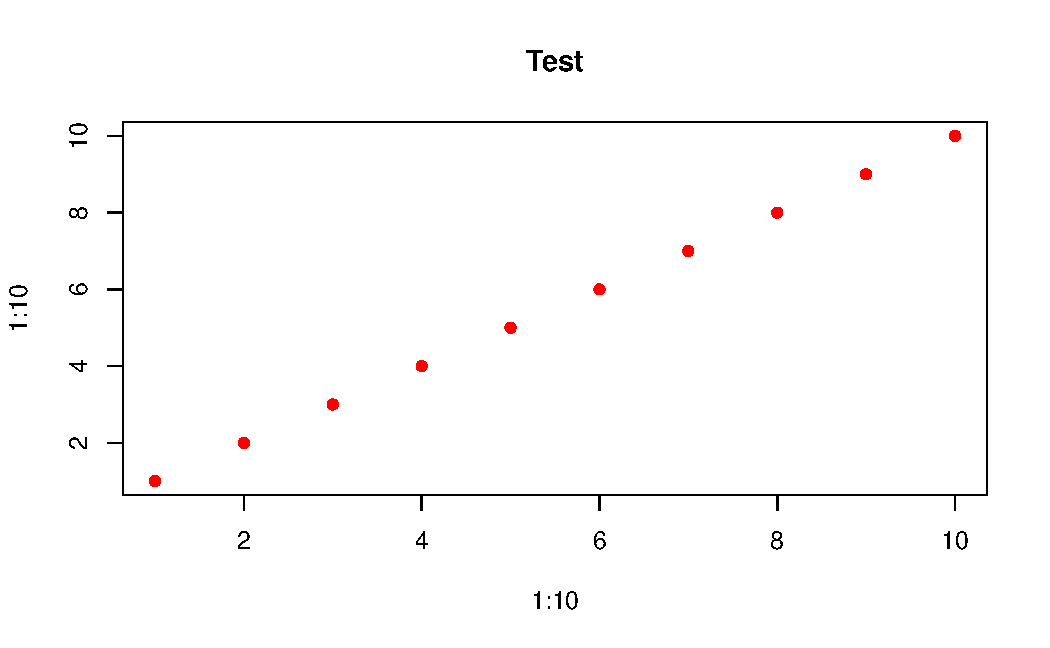
\includegraphics[width=1\linewidth]{mastering-r-through-errors_files/figure-latex/unnamed-chunk-819-1} \end{center}

\section{Documentation}\label{documentation}

🎯 \textbf{Best Practice: Document Your Functions}

\begin{Shaded}
\begin{Highlighting}[]
\CommentTok{\#\textquotesingle{} Calculate the area of a circle}
\CommentTok{\#\textquotesingle{}}
\CommentTok{\#\textquotesingle{} @param radius Numeric. The radius of the circle.}
\CommentTok{\#\textquotesingle{} @param units Character. The units of measurement (default: "cm").}
\CommentTok{\#\textquotesingle{} @return Numeric. The area of the circle.}
\CommentTok{\#\textquotesingle{} @examples}
\CommentTok{\#\textquotesingle{} circle\_area(5)}
\CommentTok{\#\textquotesingle{} circle\_area(10, units = "inches")}
\CommentTok{\#\textquotesingle{} @export}
\NormalTok{circle\_area }\OtherTok{\textless{}{-}} \ControlFlowTok{function}\NormalTok{(radius, }\AttributeTok{units =} \StringTok{"cm"}\NormalTok{) \{}
  \ControlFlowTok{if}\NormalTok{ (}\SpecialCharTok{!}\FunctionTok{is.numeric}\NormalTok{(radius) }\SpecialCharTok{||}\NormalTok{ radius }\SpecialCharTok{\textless{}} \DecValTok{0}\NormalTok{) \{}
    \FunctionTok{stop}\NormalTok{(}\StringTok{"radius must be a non{-}negative number"}\NormalTok{)}
\NormalTok{  \}}
  
\NormalTok{  area }\OtherTok{\textless{}{-}}\NormalTok{ pi }\SpecialCharTok{*}\NormalTok{ radius}\SpecialCharTok{\^{}}\DecValTok{2}
  
  \FunctionTok{structure}\NormalTok{(}
\NormalTok{    area,}
    \AttributeTok{units =}\NormalTok{ units,}
    \AttributeTok{class =} \FunctionTok{c}\NormalTok{(}\StringTok{"circle\_area"}\NormalTok{, }\StringTok{"numeric"}\NormalTok{)}
\NormalTok{  )}
\NormalTok{\}}

\CommentTok{\# In{-}function comments}
\NormalTok{calculate\_price }\OtherTok{\textless{}{-}} \ControlFlowTok{function}\NormalTok{(base\_price, }\AttributeTok{tax\_rate =} \FloatTok{0.1}\NormalTok{, }\AttributeTok{discount =} \DecValTok{0}\NormalTok{) \{}
  \CommentTok{\# Validate inputs}
  \ControlFlowTok{if}\NormalTok{ (base\_price }\SpecialCharTok{\textless{}} \DecValTok{0}\NormalTok{) }\FunctionTok{stop}\NormalTok{(}\StringTok{"base\_price cannot be negative"}\NormalTok{)}
  \ControlFlowTok{if}\NormalTok{ (tax\_rate }\SpecialCharTok{\textless{}} \DecValTok{0} \SpecialCharTok{||}\NormalTok{ tax\_rate }\SpecialCharTok{\textgreater{}} \DecValTok{1}\NormalTok{) }\FunctionTok{stop}\NormalTok{(}\StringTok{"tax\_rate must be between 0 and 1"}\NormalTok{)}
  \ControlFlowTok{if}\NormalTok{ (discount }\SpecialCharTok{\textless{}} \DecValTok{0} \SpecialCharTok{||}\NormalTok{ discount }\SpecialCharTok{\textgreater{}} \DecValTok{1}\NormalTok{) }\FunctionTok{stop}\NormalTok{(}\StringTok{"discount must be between 0 and 1"}\NormalTok{)}
  
  \CommentTok{\# Apply discount}
\NormalTok{  discounted\_price }\OtherTok{\textless{}{-}}\NormalTok{ base\_price }\SpecialCharTok{*}\NormalTok{ (}\DecValTok{1} \SpecialCharTok{{-}}\NormalTok{ discount)}
  
  \CommentTok{\# Add tax}
\NormalTok{  final\_price }\OtherTok{\textless{}{-}}\NormalTok{ discounted\_price }\SpecialCharTok{*}\NormalTok{ (}\DecValTok{1} \SpecialCharTok{+}\NormalTok{ tax\_rate)}
  
  \CommentTok{\# Return itemized result}
  \FunctionTok{list}\NormalTok{(}
    \AttributeTok{base\_price =}\NormalTok{ base\_price,}
    \AttributeTok{discount =}\NormalTok{ discount,}
    \AttributeTok{discounted\_price =}\NormalTok{ discounted\_price,}
    \AttributeTok{tax =}\NormalTok{ discounted\_price }\SpecialCharTok{*}\NormalTok{ tax\_rate,}
    \AttributeTok{final\_price =}\NormalTok{ final\_price}
\NormalTok{  )}
\NormalTok{\}}
\end{Highlighting}
\end{Shaded}

\section{Summary}\label{summary-15}

\textbf{Key Takeaways:}

\begin{enumerate}
\def\labelenumi{\arabic{enumi}.}
\tightlist
\item
  \textbf{Functions are objects} - Can be assigned, passed, returned
\item
  \textbf{could not find function} - Check spelling, loading, scope
\item
  \textbf{Provide required arguments} - Or add defaults
\item
  \textbf{Don't pass extra arguments} - Unless function uses \ldots{}
\item
  \textbf{Last expression is returned} - Or use return() explicitly
\item
  \textbf{closure not subsettable} - You're trying to subset a function
\item
  \textbf{Use \ldots{} for flexibility} - Pass extra args to other functions
\item
  \textbf{Validate inputs} - Check types and values
\end{enumerate}

\textbf{Quick Reference:}

\begin{longtable}[]{@{}
  >{\raggedright\arraybackslash}p{(\linewidth - 4\tabcolsep) * \real{0.3684}}
  >{\raggedright\arraybackslash}p{(\linewidth - 4\tabcolsep) * \real{0.3684}}
  >{\raggedright\arraybackslash}p{(\linewidth - 4\tabcolsep) * \real{0.2632}}@{}}
\toprule\noalign{}
\begin{minipage}[b]{\linewidth}\raggedright
Error
\end{minipage} & \begin{minipage}[b]{\linewidth}\raggedright
Cause
\end{minipage} & \begin{minipage}[b]{\linewidth}\raggedright
Fix
\end{minipage} \\
\midrule\noalign{}
\endhead
\bottomrule\noalign{}
\endlastfoot
could not find function & Typo, not loaded, not defined & Check spelling, load package \\
argument missing & Required arg not provided & Provide arg or add default \\
unused argument & Too many args & Remove extra or use \ldots{} \\
closure not subsettable & Subsetting a function & Call function or use right object \\
\end{longtable}

\textbf{Function Creation:}

\begin{Shaded}
\begin{Highlighting}[]
\CommentTok{\# Basic function}
\NormalTok{my\_func }\OtherTok{\textless{}{-}} \ControlFlowTok{function}\NormalTok{(x, y) \{}
\NormalTok{  x }\SpecialCharTok{+}\NormalTok{ y}
\NormalTok{\}}

\CommentTok{\# With defaults}
\NormalTok{my\_func }\OtherTok{\textless{}{-}} \ControlFlowTok{function}\NormalTok{(x, }\AttributeTok{y =} \DecValTok{0}\NormalTok{) \{}
\NormalTok{  x }\SpecialCharTok{+}\NormalTok{ y}
\NormalTok{\}}

\CommentTok{\# With ...}
\NormalTok{my\_func }\OtherTok{\textless{}{-}} \ControlFlowTok{function}\NormalTok{(x, ...) \{}
  \CommentTok{\# Do something}
  \FunctionTok{other\_func}\NormalTok{(x, ...)}
\NormalTok{\}}

\CommentTok{\# With validation}
\NormalTok{my\_func }\OtherTok{\textless{}{-}} \ControlFlowTok{function}\NormalTok{(x) \{}
  \ControlFlowTok{if}\NormalTok{ (}\SpecialCharTok{!}\FunctionTok{is.numeric}\NormalTok{(x)) }\FunctionTok{stop}\NormalTok{(}\StringTok{"x must be numeric"}\NormalTok{)}
\NormalTok{  x }\SpecialCharTok{*} \DecValTok{2}
\NormalTok{\}}

\CommentTok{\# Return values}
\NormalTok{my\_func }\OtherTok{\textless{}{-}} \ControlFlowTok{function}\NormalTok{(x) \{}
  \FunctionTok{list}\NormalTok{(}\AttributeTok{result =}\NormalTok{ x }\SpecialCharTok{*} \DecValTok{2}\NormalTok{, }\AttributeTok{original =}\NormalTok{ x)}
\NormalTok{\}}
\end{Highlighting}
\end{Shaded}

\textbf{Best Practices:}

\begin{Shaded}
\begin{Highlighting}[]
\CommentTok{\# ✅ Good}
\ControlFlowTok{function}\NormalTok{(x, }\AttributeTok{y =} \DecValTok{0}\NormalTok{)              }\CommentTok{\# Sensible defaults}
\ControlFlowTok{if}\NormalTok{ (}\SpecialCharTok{!}\FunctionTok{is.numeric}\NormalTok{(x)) }\FunctionTok{stop}\NormalTok{()      }\CommentTok{\# Validate inputs}
\FunctionTok{return}\NormalTok{(}\FunctionTok{list}\NormalTok{(}\AttributeTok{a =} \DecValTok{1}\NormalTok{, }\AttributeTok{b =} \DecValTok{2}\NormalTok{))      }\CommentTok{\# Multiple values in list}
\NormalTok{Use descriptive names            }\CommentTok{\# clear\_cache() not cc()}

\CommentTok{\# ❌ Avoid}
\ControlFlowTok{function}\NormalTok{(x)                     }\CommentTok{\# No defaults when optional}
\NormalTok{No input validation             }\CommentTok{\# Causes cryptic errors later}
\NormalTok{mean }\OtherTok{\textless{}{-}}\NormalTok{ my\_data                 }\CommentTok{\# Overwriting function names}
\ControlFlowTok{function}\NormalTok{(x, y, z, a, b, c)      }\CommentTok{\# Too many arguments}
\end{Highlighting}
\end{Shaded}

\section{Exercises}\label{exercises-15}

📝 \textbf{Exercise 1: Safe Division Function}

Write \texttt{safe\_divide(x,\ y)} that:
1. Checks both are numeric
2. Handles division by zero
3. Works with vectors
4. Returns informative errors

📝 \textbf{Exercise 2: Flexible Summary}

Write \texttt{my\_summary(x,\ ...)} that:
1. Calculates mean, median, sd
2. Accepts \ldots{} for additional stats
3. Handles NA values
4. Returns named list

📝 \textbf{Exercise 3: Argument Validator}

Write \texttt{validate\_args(func,\ ...)} that:
1. Checks if function exists
2. Validates argument types
3. Checks required args provided
4. Returns TRUE/FALSE with messages

📝 \textbf{Exercise 4: Function Factory}

Write \texttt{make\_adder(n)} that returns a function that adds n to its argument.

Example:

\begin{Shaded}
\begin{Highlighting}[]
\NormalTok{add\_5 }\OtherTok{\textless{}{-}} \FunctionTok{make\_adder}\NormalTok{(}\DecValTok{5}\NormalTok{)}
\FunctionTok{add\_5}\NormalTok{(}\DecValTok{10}\NormalTok{)  }\CommentTok{\# Should return 15}
\end{Highlighting}
\end{Shaded}

\section{Exercise Answers}\label{exercise-answers-15}

Click to see answers

\textbf{Exercise 1:}

\begin{Shaded}
\begin{Highlighting}[]
\NormalTok{safe\_divide }\OtherTok{\textless{}{-}} \ControlFlowTok{function}\NormalTok{(x, y) \{}
  \CommentTok{\# Check types}
  \ControlFlowTok{if}\NormalTok{ (}\SpecialCharTok{!}\FunctionTok{is.numeric}\NormalTok{(x)) \{}
    \FunctionTok{stop}\NormalTok{(}\StringTok{"x must be numeric, got "}\NormalTok{, }\FunctionTok{class}\NormalTok{(x)[}\DecValTok{1}\NormalTok{])}
\NormalTok{  \}}
  \ControlFlowTok{if}\NormalTok{ (}\SpecialCharTok{!}\FunctionTok{is.numeric}\NormalTok{(y)) \{}
    \FunctionTok{stop}\NormalTok{(}\StringTok{"y must be numeric, got "}\NormalTok{, }\FunctionTok{class}\NormalTok{(y)[}\DecValTok{1}\NormalTok{])}
\NormalTok{  \}}
  
  \CommentTok{\# Check for zero}
  \ControlFlowTok{if}\NormalTok{ (}\FunctionTok{any}\NormalTok{(y }\SpecialCharTok{==} \DecValTok{0}\NormalTok{)) \{}
    \FunctionTok{warning}\NormalTok{(}\StringTok{"Division by zero detected, returning Inf/{-}Inf"}\NormalTok{)}
    \CommentTok{\# R handles this naturally, but we warn}
\NormalTok{  \}}
  
  \CommentTok{\# Check lengths match or can recycle}
  \ControlFlowTok{if}\NormalTok{ (}\FunctionTok{length}\NormalTok{(x) }\SpecialCharTok{!=} \FunctionTok{length}\NormalTok{(y) }\SpecialCharTok{\&\&} \FunctionTok{length}\NormalTok{(x) }\SpecialCharTok{!=} \DecValTok{1} \SpecialCharTok{\&\&} \FunctionTok{length}\NormalTok{(y) }\SpecialCharTok{!=} \DecValTok{1}\NormalTok{) \{}
    \ControlFlowTok{if}\NormalTok{ (}\FunctionTok{max}\NormalTok{(}\FunctionTok{length}\NormalTok{(x), }\FunctionTok{length}\NormalTok{(y)) }\SpecialCharTok{\%\%} \FunctionTok{min}\NormalTok{(}\FunctionTok{length}\NormalTok{(x), }\FunctionTok{length}\NormalTok{(y)) }\SpecialCharTok{!=} \DecValTok{0}\NormalTok{) \{}
      \FunctionTok{warning}\NormalTok{(}\StringTok{"Lengths not compatible for recycling: "}\NormalTok{,}
              \FunctionTok{length}\NormalTok{(x), }\StringTok{" and "}\NormalTok{, }\FunctionTok{length}\NormalTok{(y))}
\NormalTok{    \}}
\NormalTok{  \}}
  
\NormalTok{  result }\OtherTok{\textless{}{-}}\NormalTok{ x }\SpecialCharTok{/}\NormalTok{ y}
\NormalTok{  result}
\NormalTok{\}}

\CommentTok{\# Test}
\FunctionTok{safe\_divide}\NormalTok{(}\DecValTok{10}\NormalTok{, }\DecValTok{2}\NormalTok{)}
\CommentTok{\#\textgreater{} [1] 5}
\FunctionTok{safe\_divide}\NormalTok{(}\FunctionTok{c}\NormalTok{(}\DecValTok{10}\NormalTok{, }\DecValTok{20}\NormalTok{, }\DecValTok{30}\NormalTok{), }\FunctionTok{c}\NormalTok{(}\DecValTok{2}\NormalTok{, }\DecValTok{4}\NormalTok{, }\DecValTok{5}\NormalTok{))}
\CommentTok{\#\textgreater{} [1] 5 5 6}
\FunctionTok{safe\_divide}\NormalTok{(}\DecValTok{10}\NormalTok{, }\DecValTok{0}\NormalTok{)  }\CommentTok{\# Warning}
\CommentTok{\#\textgreater{} Warning in safe\_divide(10, 0): Division by zero detected, returning Inf/{-}Inf}
\CommentTok{\#\textgreater{} [1] Inf}
\end{Highlighting}
\end{Shaded}

\begin{Shaded}
\begin{Highlighting}[]
\FunctionTok{safe\_divide}\NormalTok{(}\StringTok{"10"}\NormalTok{, }\DecValTok{2}\NormalTok{)  }\CommentTok{\# Error}
\CommentTok{\#\textgreater{} Error in safe\_divide("10", 2): x must be numeric, got character}
\end{Highlighting}
\end{Shaded}

\textbf{Exercise 2:}

\begin{Shaded}
\begin{Highlighting}[]
\NormalTok{my\_summary }\OtherTok{\textless{}{-}} \ControlFlowTok{function}\NormalTok{(x, ..., }\AttributeTok{na.rm =} \ConstantTok{TRUE}\NormalTok{) \{}
  \CommentTok{\# Base statistics}
\NormalTok{  result }\OtherTok{\textless{}{-}} \FunctionTok{list}\NormalTok{(}
    \AttributeTok{n =} \FunctionTok{length}\NormalTok{(x),}
    \AttributeTok{n\_missing =} \FunctionTok{sum}\NormalTok{(}\FunctionTok{is.na}\NormalTok{(x)),}
    \AttributeTok{mean =} \FunctionTok{mean}\NormalTok{(x, }\AttributeTok{na.rm =}\NormalTok{ na.rm),}
    \AttributeTok{median =} \FunctionTok{median}\NormalTok{(x, }\AttributeTok{na.rm =}\NormalTok{ na.rm),}
    \AttributeTok{sd =} \FunctionTok{sd}\NormalTok{(x, }\AttributeTok{na.rm =}\NormalTok{ na.rm),}
    \AttributeTok{min =} \FunctionTok{min}\NormalTok{(x, }\AttributeTok{na.rm =}\NormalTok{ na.rm),}
    \AttributeTok{max =} \FunctionTok{max}\NormalTok{(x, }\AttributeTok{na.rm =}\NormalTok{ na.rm)}
\NormalTok{  )}
  
  \CommentTok{\# Additional statistics from ...}
\NormalTok{  extra\_stats }\OtherTok{\textless{}{-}} \FunctionTok{list}\NormalTok{(...)}
  
  \ControlFlowTok{for}\NormalTok{ (stat\_name }\ControlFlowTok{in} \FunctionTok{names}\NormalTok{(extra\_stats)) \{}
\NormalTok{    stat\_func }\OtherTok{\textless{}{-}}\NormalTok{ extra\_stats[[stat\_name]]}
    \ControlFlowTok{if}\NormalTok{ (}\FunctionTok{is.function}\NormalTok{(stat\_func)) \{}
\NormalTok{      result[[stat\_name]] }\OtherTok{\textless{}{-}} \FunctionTok{stat\_func}\NormalTok{(x, }\AttributeTok{na.rm =}\NormalTok{ na.rm)}
\NormalTok{    \}}
\NormalTok{  \}}
  
  \FunctionTok{class}\NormalTok{(result) }\OtherTok{\textless{}{-}} \StringTok{"my\_summary"}
\NormalTok{  result}
\NormalTok{\}}

\CommentTok{\# Print method}
\NormalTok{print.my\_summary }\OtherTok{\textless{}{-}} \ControlFlowTok{function}\NormalTok{(x, ...) \{}
  \FunctionTok{cat}\NormalTok{(}\StringTok{"Summary Statistics}\SpecialCharTok{\textbackslash{}n}\StringTok{"}\NormalTok{)}
  \FunctionTok{cat}\NormalTok{(}\StringTok{"==================}\SpecialCharTok{\textbackslash{}n}\StringTok{"}\NormalTok{)}
  \ControlFlowTok{for}\NormalTok{ (name }\ControlFlowTok{in} \FunctionTok{names}\NormalTok{(x)) \{}
    \FunctionTok{cat}\NormalTok{(}\FunctionTok{sprintf}\NormalTok{(}\StringTok{"\%{-}12s: \%s}\SpecialCharTok{\textbackslash{}n}\StringTok{"}\NormalTok{, name, }
                \FunctionTok{format}\NormalTok{(x[[name]], }\AttributeTok{digits =} \DecValTok{3}\NormalTok{)))}
\NormalTok{  \}}
  \FunctionTok{invisible}\NormalTok{(x)}
\NormalTok{\}}

\CommentTok{\# Test}
\NormalTok{data }\OtherTok{\textless{}{-}} \FunctionTok{c}\NormalTok{(}\DecValTok{1}\NormalTok{, }\DecValTok{2}\NormalTok{, }\ConstantTok{NA}\NormalTok{, }\DecValTok{4}\NormalTok{, }\DecValTok{5}\NormalTok{, }\DecValTok{6}\NormalTok{, }\DecValTok{7}\NormalTok{, }\DecValTok{8}\NormalTok{, }\DecValTok{9}\NormalTok{, }\DecValTok{10}\NormalTok{)}
\FunctionTok{my\_summary}\NormalTok{(data)}
\CommentTok{\#\textgreater{} Summary Statistics}
\CommentTok{\#\textgreater{} ==================}
\CommentTok{\#\textgreater{} n           : 10}
\CommentTok{\#\textgreater{} n\_missing   : 1}
\CommentTok{\#\textgreater{} mean        : 5.78}
\CommentTok{\#\textgreater{} median      : 6}
\CommentTok{\#\textgreater{} sd          : 3.07}
\CommentTok{\#\textgreater{} min         : 1}
\CommentTok{\#\textgreater{} max         : 10}

\CommentTok{\# With extra stats}
\FunctionTok{my\_summary}\NormalTok{(data, }
          \AttributeTok{IQR =}\NormalTok{ IQR,}
          \AttributeTok{mad =}\NormalTok{ mad)}
\CommentTok{\#\textgreater{} Summary Statistics}
\CommentTok{\#\textgreater{} ==================}
\CommentTok{\#\textgreater{} n           : 10}
\CommentTok{\#\textgreater{} n\_missing   : 1}
\CommentTok{\#\textgreater{} mean        : 5.78}
\CommentTok{\#\textgreater{} median      : 6}
\CommentTok{\#\textgreater{} sd          : 3.07}
\CommentTok{\#\textgreater{} min         : 1}
\CommentTok{\#\textgreater{} max         : 10}
\CommentTok{\#\textgreater{} IQR         : 4}
\CommentTok{\#\textgreater{} mad         : 2.97}
\end{Highlighting}
\end{Shaded}

\textbf{Exercise 3:}

\begin{Shaded}
\begin{Highlighting}[]
\NormalTok{validate\_args }\OtherTok{\textless{}{-}} \ControlFlowTok{function}\NormalTok{(func\_name, ...) \{}
  \CommentTok{\# Check function exists}
  \ControlFlowTok{if}\NormalTok{ (}\SpecialCharTok{!}\FunctionTok{exists}\NormalTok{(func\_name, }\AttributeTok{mode =} \StringTok{"function"}\NormalTok{)) \{}
    \FunctionTok{message}\NormalTok{(}\StringTok{"✗ Function \textquotesingle{}"}\NormalTok{, func\_name, }\StringTok{"\textquotesingle{} not found"}\NormalTok{)}
    \FunctionTok{return}\NormalTok{(}\ConstantTok{FALSE}\NormalTok{)}
\NormalTok{  \}}
  
\NormalTok{  func }\OtherTok{\textless{}{-}} \FunctionTok{get}\NormalTok{(func\_name, }\AttributeTok{mode =} \StringTok{"function"}\NormalTok{)}
\NormalTok{  func\_args }\OtherTok{\textless{}{-}} \FunctionTok{formals}\NormalTok{(func)}
  
  \CommentTok{\# Get provided arguments}
\NormalTok{  provided }\OtherTok{\textless{}{-}} \FunctionTok{list}\NormalTok{(...)}
  
  \CommentTok{\# Check required arguments (those without defaults)}
\NormalTok{  required\_args }\OtherTok{\textless{}{-}} \FunctionTok{names}\NormalTok{(func\_args)[}\FunctionTok{sapply}\NormalTok{(func\_args, }
                                           \ControlFlowTok{function}\NormalTok{(x) }\FunctionTok{class}\NormalTok{(x) }\SpecialCharTok{==} \StringTok{"name"}\NormalTok{)]}
  
\NormalTok{  missing\_required }\OtherTok{\textless{}{-}} \FunctionTok{setdiff}\NormalTok{(required\_args, }\FunctionTok{names}\NormalTok{(provided))}
  
  \ControlFlowTok{if}\NormalTok{ (}\FunctionTok{length}\NormalTok{(missing\_required) }\SpecialCharTok{\textgreater{}} \DecValTok{0}\NormalTok{) \{}
    \FunctionTok{message}\NormalTok{(}\StringTok{"✗ Missing required arguments: "}\NormalTok{, }
            \FunctionTok{paste}\NormalTok{(missing\_required, }\AttributeTok{collapse =} \StringTok{", "}\NormalTok{))}
    \FunctionTok{return}\NormalTok{(}\ConstantTok{FALSE}\NormalTok{)}
\NormalTok{  \}}
  
  \CommentTok{\# Check for unexpected arguments}
  \ControlFlowTok{if}\NormalTok{ (}\SpecialCharTok{!}\StringTok{"..."} \SpecialCharTok{\%in\%} \FunctionTok{names}\NormalTok{(func\_args)) \{}
\NormalTok{    unexpected }\OtherTok{\textless{}{-}} \FunctionTok{setdiff}\NormalTok{(}\FunctionTok{names}\NormalTok{(provided), }\FunctionTok{names}\NormalTok{(func\_args))}
    \ControlFlowTok{if}\NormalTok{ (}\FunctionTok{length}\NormalTok{(unexpected) }\SpecialCharTok{\textgreater{}} \DecValTok{0}\NormalTok{) \{}
      \FunctionTok{message}\NormalTok{(}\StringTok{"✗ Unexpected arguments: "}\NormalTok{, }
              \FunctionTok{paste}\NormalTok{(unexpected, }\AttributeTok{collapse =} \StringTok{", "}\NormalTok{))}
      \FunctionTok{return}\NormalTok{(}\ConstantTok{FALSE}\NormalTok{)}
\NormalTok{    \}}
\NormalTok{  \}}
  
  \CommentTok{\# Check argument types (basic)}
  \ControlFlowTok{for}\NormalTok{ (arg\_name }\ControlFlowTok{in} \FunctionTok{names}\NormalTok{(provided)) \{}
\NormalTok{    arg\_value }\OtherTok{\textless{}{-}}\NormalTok{ provided[[arg\_name]]}
    \CommentTok{\# Could add more sophisticated type checking here}
\NormalTok{  \}}
  
  \FunctionTok{message}\NormalTok{(}\StringTok{"✓ All validations passed for \textquotesingle{}"}\NormalTok{, func\_name, }\StringTok{"\textquotesingle{}"}\NormalTok{)}
  \FunctionTok{return}\NormalTok{(}\ConstantTok{TRUE}\NormalTok{)}
\NormalTok{\}}

\CommentTok{\# Test}
\FunctionTok{validate\_args}\NormalTok{(}\StringTok{"mean"}\NormalTok{, }\AttributeTok{x =} \FunctionTok{c}\NormalTok{(}\DecValTok{1}\NormalTok{, }\DecValTok{2}\NormalTok{, }\DecValTok{3}\NormalTok{), }\AttributeTok{na.rm =} \ConstantTok{TRUE}\NormalTok{)}
\CommentTok{\#\textgreater{} ✗ Missing required arguments: ...}
\CommentTok{\#\textgreater{} [1] FALSE}
\FunctionTok{validate\_args}\NormalTok{(}\StringTok{"mean"}\NormalTok{, }\AttributeTok{na.rm =} \ConstantTok{TRUE}\NormalTok{)  }\CommentTok{\# Missing x}
\CommentTok{\#\textgreater{} ✗ Missing required arguments: x, ...}
\CommentTok{\#\textgreater{} [1] FALSE}
\FunctionTok{validate\_args}\NormalTok{(}\StringTok{"mean"}\NormalTok{, }\AttributeTok{x =} \FunctionTok{c}\NormalTok{(}\DecValTok{1}\NormalTok{, }\DecValTok{2}\NormalTok{, }\DecValTok{3}\NormalTok{), }\AttributeTok{invalid =} \ConstantTok{TRUE}\NormalTok{)  }\CommentTok{\# Extra arg}
\CommentTok{\#\textgreater{} ✗ Missing required arguments: ...}
\CommentTok{\#\textgreater{} [1] FALSE}
\end{Highlighting}
\end{Shaded}

\textbf{Exercise 4:}

\begin{Shaded}
\begin{Highlighting}[]
\NormalTok{make\_adder }\OtherTok{\textless{}{-}} \ControlFlowTok{function}\NormalTok{(n) \{}
  \CommentTok{\# Return a function that adds n}
  \ControlFlowTok{function}\NormalTok{(x) \{}
\NormalTok{    x }\SpecialCharTok{+}\NormalTok{ n}
\NormalTok{  \}}
\NormalTok{\}}

\CommentTok{\# Test}
\NormalTok{add\_5 }\OtherTok{\textless{}{-}} \FunctionTok{make\_adder}\NormalTok{(}\DecValTok{5}\NormalTok{)}
\FunctionTok{add\_5}\NormalTok{(}\DecValTok{10}\NormalTok{)}
\CommentTok{\#\textgreater{} [1] 15}

\NormalTok{add\_100 }\OtherTok{\textless{}{-}} \FunctionTok{make\_adder}\NormalTok{(}\DecValTok{100}\NormalTok{)}
\FunctionTok{add\_100}\NormalTok{(}\DecValTok{50}\NormalTok{)}
\CommentTok{\#\textgreater{} [1] 150}

\CommentTok{\# Multiple uses}
\FunctionTok{add\_5}\NormalTok{(}\DecValTok{1}\SpecialCharTok{:}\DecValTok{10}\NormalTok{)}
\CommentTok{\#\textgreater{}  [1]  6  7  8  9 10 11 12 13 14 15}

\CommentTok{\# Each function retains its own n}
\FunctionTok{add\_5}\NormalTok{(}\DecValTok{5}\NormalTok{)}
\CommentTok{\#\textgreater{} [1] 10}
\FunctionTok{add\_100}\NormalTok{(}\DecValTok{5}\NormalTok{)}
\CommentTok{\#\textgreater{} [1] 105}

\CommentTok{\# More advanced: with validation}
\NormalTok{make\_adder\_safe }\OtherTok{\textless{}{-}} \ControlFlowTok{function}\NormalTok{(n) \{}
  \ControlFlowTok{if}\NormalTok{ (}\SpecialCharTok{!}\FunctionTok{is.numeric}\NormalTok{(n) }\SpecialCharTok{||} \FunctionTok{length}\NormalTok{(n) }\SpecialCharTok{!=} \DecValTok{1}\NormalTok{) \{}
    \FunctionTok{stop}\NormalTok{(}\StringTok{"n must be a single numeric value"}\NormalTok{)}
\NormalTok{  \}}
  
  \ControlFlowTok{function}\NormalTok{(x) \{}
    \ControlFlowTok{if}\NormalTok{ (}\SpecialCharTok{!}\FunctionTok{is.numeric}\NormalTok{(x)) \{}
      \FunctionTok{stop}\NormalTok{(}\StringTok{"x must be numeric"}\NormalTok{)}
\NormalTok{    \}}
\NormalTok{    x }\SpecialCharTok{+}\NormalTok{ n}
\NormalTok{  \}}
\NormalTok{\}}

\NormalTok{add\_3 }\OtherTok{\textless{}{-}} \FunctionTok{make\_adder\_safe}\NormalTok{(}\DecValTok{3}\NormalTok{)}
\FunctionTok{add\_3}\NormalTok{(}\DecValTok{10}\NormalTok{)}
\CommentTok{\#\textgreater{} [1] 13}
\end{Highlighting}
\end{Shaded}

\chapter{Scoping \& Environments}\label{scoping-environments}

\textbf{What You'll Learn:}

\begin{itemize}
\tightlist
\item
  How R finds objects
\item
  Lexical scoping rules
\item
  Environment hierarchy
\item
  Common scoping errors
\item
  Global vs local variables
\end{itemize}

\textbf{Key Errors Covered:} 12+ scoping errors

\textbf{Difficulty:} ⭐⭐⭐ Advanced

\section{Introduction}\label{introduction-16}

Scoping determines how R finds objects, and it's often surprising:

\begin{Shaded}
\begin{Highlighting}[]
\NormalTok{x }\OtherTok{\textless{}{-}} \DecValTok{10}

\NormalTok{my\_func }\OtherTok{\textless{}{-}} \ControlFlowTok{function}\NormalTok{() \{}
\NormalTok{  x  }\CommentTok{\# Where does this x come from?}
\NormalTok{\}}

\FunctionTok{my\_func}\NormalTok{()  }\CommentTok{\# Returns 10!}
\CommentTok{\#\textgreater{} [1] 10}
\end{Highlighting}
\end{Shaded}

Let's understand scoping to avoid confusion.

\section{Environment Basics}\label{environment-basics}

💡 \textbf{Key Insight: Environments Are Like Named Lists}

\begin{Shaded}
\begin{Highlighting}[]
\CommentTok{\# Create an environment}
\NormalTok{my\_env }\OtherTok{\textless{}{-}} \FunctionTok{new.env}\NormalTok{()}

\CommentTok{\# Add objects}
\NormalTok{my\_env}\SpecialCharTok{$}\NormalTok{x }\OtherTok{\textless{}{-}} \DecValTok{10}
\NormalTok{my\_env}\SpecialCharTok{$}\NormalTok{y }\OtherTok{\textless{}{-}} \DecValTok{20}

\CommentTok{\# Access objects}
\NormalTok{my\_env}\SpecialCharTok{$}\NormalTok{x}
\CommentTok{\#\textgreater{} [1] 10}

\CommentTok{\# List contents}
\FunctionTok{ls}\NormalTok{(my\_env)}
\CommentTok{\#\textgreater{} [1] "x" "y"}

\CommentTok{\# Every function has an environment}
\NormalTok{f }\OtherTok{\textless{}{-}} \ControlFlowTok{function}\NormalTok{() \{}
\NormalTok{  x }\OtherTok{\textless{}{-}} \DecValTok{5}
  \FunctionTok{environment}\NormalTok{()}
\NormalTok{\}}

\NormalTok{f\_env }\OtherTok{\textless{}{-}} \FunctionTok{f}\NormalTok{()}
\FunctionTok{ls}\NormalTok{(f\_env)}
\CommentTok{\#\textgreater{} [1] "x"}

\CommentTok{\# Current environment}
\FunctionTok{environment}\NormalTok{()  }\CommentTok{\# Usually global environment}
\CommentTok{\#\textgreater{} \textless{}environment: R\_GlobalEnv\textgreater{}}

\CommentTok{\# Parent environment}
\FunctionTok{parent.env}\NormalTok{(my\_env)}
\CommentTok{\#\textgreater{} \textless{}environment: R\_GlobalEnv\textgreater{}}
\end{Highlighting}
\end{Shaded}

\textbf{Key points:}
- Environments contain named objects
- Every function creates a new environment
- Environments have parents
- R searches up the chain

\section{\texorpdfstring{Error \#1: \texttt{object\ not\ found} (scoping)}{Error \#1: object not found (scoping)}}\label{object-not-found-scope}

{⭐⭐ INTERMEDIATE} {🔍 SCOPE}

\subsection{The Error}\label{the-error-67}

\begin{Shaded}
\begin{Highlighting}[]
\NormalTok{my\_func }\OtherTok{\textless{}{-}} \ControlFlowTok{function}\NormalTok{() \{}
\NormalTok{  y }\OtherTok{\textless{}{-}} \DecValTok{20}
\NormalTok{\}}

\FunctionTok{my\_func}\NormalTok{()}

\NormalTok{y  }\CommentTok{\# Where is y?}
\CommentTok{\#\textgreater{} [1] "1 items" "2 items" "3 items"}
\end{Highlighting}
\end{Shaded}

🔴 \textbf{ERROR}

\begin{verbatim}
Error in eval(expr, envir, enclos) : object 'y' not found
\end{verbatim}

\subsection{What It Means}\label{what-it-means-72}

The object was created in a function's environment and isn't accessible outside.

\subsection{Understanding Scope}\label{understanding-scope}

\begin{Shaded}
\begin{Highlighting}[]
\CommentTok{\# Global scope}
\NormalTok{x }\OtherTok{\textless{}{-}} \DecValTok{10}

\NormalTok{func1 }\OtherTok{\textless{}{-}} \ControlFlowTok{function}\NormalTok{() \{}
  \CommentTok{\# Function scope}
\NormalTok{  y }\OtherTok{\textless{}{-}} \DecValTok{20}
  
  \CommentTok{\# Can see global x}
  \FunctionTok{cat}\NormalTok{(}\StringTok{"x:"}\NormalTok{, x, }\StringTok{"}\SpecialCharTok{\textbackslash{}n}\StringTok{"}\NormalTok{)}
  
  \CommentTok{\# Can see local y}
  \FunctionTok{cat}\NormalTok{(}\StringTok{"y:"}\NormalTok{, y, }\StringTok{"}\SpecialCharTok{\textbackslash{}n}\StringTok{"}\NormalTok{)}
\NormalTok{\}}

\FunctionTok{func1}\NormalTok{()}
\CommentTok{\#\textgreater{} x: 10 }
\CommentTok{\#\textgreater{} y: 20}

\CommentTok{\# x exists globally}
\NormalTok{x}
\CommentTok{\#\textgreater{} [1] 10}

\CommentTok{\# y doesn\textquotesingle{}t (was in function scope)}
\FunctionTok{exists}\NormalTok{(}\StringTok{"y"}\NormalTok{)  }\CommentTok{\# FALSE}
\CommentTok{\#\textgreater{} [1] TRUE}

\CommentTok{\# Example 2: Nested functions}
\NormalTok{outer\_func }\OtherTok{\textless{}{-}} \ControlFlowTok{function}\NormalTok{() \{}
\NormalTok{  z }\OtherTok{\textless{}{-}} \DecValTok{30}
  
\NormalTok{  inner\_func }\OtherTok{\textless{}{-}} \ControlFlowTok{function}\NormalTok{() \{}
    \CommentTok{\# Can see z from parent environment}
\NormalTok{    z}
\NormalTok{  \}}
  
  \FunctionTok{inner\_func}\NormalTok{()}
\NormalTok{\}}

\FunctionTok{outer\_func}\NormalTok{()}
\CommentTok{\#\textgreater{} [1] 30}

\CommentTok{\# z doesn\textquotesingle{}t exist here}
\FunctionTok{exists}\NormalTok{(}\StringTok{"z"}\NormalTok{)  }\CommentTok{\# FALSE}
\CommentTok{\#\textgreater{} [1] TRUE}
\end{Highlighting}
\end{Shaded}

\subsection{Common Causes}\label{common-causes-47}

\subsubsection{Cause 1: Expecting Function to Modify Global}\label{cause-1-expecting-function-to-modify-global}

\begin{Shaded}
\begin{Highlighting}[]
\NormalTok{x }\OtherTok{\textless{}{-}} \DecValTok{10}

\CommentTok{\# This doesn\textquotesingle{}t modify global x!}
\NormalTok{add\_ten }\OtherTok{\textless{}{-}} \ControlFlowTok{function}\NormalTok{() \{}
\NormalTok{  x }\OtherTok{\textless{}{-}}\NormalTok{ x }\SpecialCharTok{+} \DecValTok{10}
\NormalTok{  x  }\CommentTok{\# Returns 20}
\NormalTok{\}}

\FunctionTok{add\_ten}\NormalTok{()  }\CommentTok{\# Returns 20}
\CommentTok{\#\textgreater{} [1] 20}
\NormalTok{x          }\CommentTok{\# Still 10!}
\CommentTok{\#\textgreater{} [1] 10}
\end{Highlighting}
\end{Shaded}

\subsubsection{Cause 2: Variables Only Exist in Loop Scope}\label{cause-2-variables-only-exist-in-loop-scope}

\begin{Shaded}
\begin{Highlighting}[]
\ControlFlowTok{for}\NormalTok{ (i }\ControlFlowTok{in} \DecValTok{1}\SpecialCharTok{:}\DecValTok{5}\NormalTok{) \{}
\NormalTok{  temp }\OtherTok{\textless{}{-}}\NormalTok{ i }\SpecialCharTok{*} \DecValTok{2}
\NormalTok{\}}

\CommentTok{\# temp still exists (for loop doesn\textquotesingle{}t create new scope in R)}
\NormalTok{temp}
\CommentTok{\#\textgreater{} [1] 10}

\CommentTok{\# But function scope is different}
\NormalTok{func }\OtherTok{\textless{}{-}} \ControlFlowTok{function}\NormalTok{() \{}
  \ControlFlowTok{for}\NormalTok{ (i }\ControlFlowTok{in} \DecValTok{1}\SpecialCharTok{:}\DecValTok{5}\NormalTok{) \{}
\NormalTok{    temp2 }\OtherTok{\textless{}{-}}\NormalTok{ i }\SpecialCharTok{*} \DecValTok{2}
\NormalTok{  \}}
\NormalTok{\}}
\FunctionTok{func}\NormalTok{()}

\NormalTok{temp2  }\CommentTok{\# Doesn\textquotesingle{}t exist}
\CommentTok{\#\textgreater{} Error: object \textquotesingle{}temp2\textquotesingle{} not found}
\end{Highlighting}
\end{Shaded}

\subsection{Solutions}\label{solutions-76}

✅ \textbf{SOLUTION 1: Return Values}

\begin{Shaded}
\begin{Highlighting}[]
\NormalTok{x }\OtherTok{\textless{}{-}} \DecValTok{10}

\CommentTok{\# Return the new value}
\NormalTok{add\_ten }\OtherTok{\textless{}{-}} \ControlFlowTok{function}\NormalTok{(val) \{}
\NormalTok{  val }\SpecialCharTok{+} \DecValTok{10}
\NormalTok{\}}

\CommentTok{\# Assign result}
\NormalTok{x }\OtherTok{\textless{}{-}} \FunctionTok{add\_ten}\NormalTok{(x)}
\NormalTok{x  }\CommentTok{\# Now 20}
\CommentTok{\#\textgreater{} [1] 20}
\end{Highlighting}
\end{Shaded}

✅ \textbf{SOLUTION 2: Use \textless\textless- for Global Assignment (Caution!)}

\begin{Shaded}
\begin{Highlighting}[]
\NormalTok{x }\OtherTok{\textless{}{-}} \DecValTok{10}

\CommentTok{\# Modifies global x}
\NormalTok{add\_ten\_global }\OtherTok{\textless{}{-}} \ControlFlowTok{function}\NormalTok{() \{}
\NormalTok{  x }\OtherTok{\textless{}\textless{}{-}}\NormalTok{ x }\SpecialCharTok{+} \DecValTok{10}
\NormalTok{\}}

\FunctionTok{add\_ten\_global}\NormalTok{()}
\NormalTok{x  }\CommentTok{\# Now 20}
\CommentTok{\#\textgreater{} [1] 20}

\CommentTok{\# ⚠️ Use sparingly! Can cause confusion}
\end{Highlighting}
\end{Shaded}

✅ \textbf{SOLUTION 3: Pass and Return Explicitly}

\begin{Shaded}
\begin{Highlighting}[]
\CommentTok{\# Best practice: explicit in and out}
\NormalTok{process\_data }\OtherTok{\textless{}{-}} \ControlFlowTok{function}\NormalTok{(data, operation) \{}
  \CommentTok{\# Do something}
\NormalTok{  result }\OtherTok{\textless{}{-}}\NormalTok{ data }\SpecialCharTok{*}\NormalTok{ operation}
  
  \CommentTok{\# Return explicitly}
  \FunctionTok{return}\NormalTok{(result)}
\NormalTok{\}}

\NormalTok{my\_data }\OtherTok{\textless{}{-}} \DecValTok{100}
\NormalTok{my\_data }\OtherTok{\textless{}{-}} \FunctionTok{process\_data}\NormalTok{(my\_data, }\DecValTok{2}\NormalTok{)}
\NormalTok{my\_data}
\CommentTok{\#\textgreater{} [1] 200}
\end{Highlighting}
\end{Shaded}

\section{Lexical Scoping}\label{lexical-scoping}

💡 \textbf{Key Insight: Lexical Scoping}

R uses lexical (static) scoping: where a function was \textbf{defined} matters, not where it's \textbf{called}.

\begin{Shaded}
\begin{Highlighting}[]
\NormalTok{x }\OtherTok{\textless{}{-}} \DecValTok{10}

\NormalTok{func1 }\OtherTok{\textless{}{-}} \ControlFlowTok{function}\NormalTok{() \{}
\NormalTok{  x  }\CommentTok{\# Uses x from where function was defined}
\NormalTok{\}}

\NormalTok{func2 }\OtherTok{\textless{}{-}} \ControlFlowTok{function}\NormalTok{() \{}
\NormalTok{  x }\OtherTok{\textless{}{-}} \DecValTok{20}  \CommentTok{\# Different x}
  \FunctionTok{func1}\NormalTok{()  }\CommentTok{\# What does this return?}
\NormalTok{\}}

\FunctionTok{func2}\NormalTok{()  }\CommentTok{\# Returns 10 (not 20!)}
\CommentTok{\#\textgreater{} [1] 10}

\CommentTok{\# Why? func1 looks for x where it was defined (global env)}
\CommentTok{\# Not where it was called (inside func2)}

\CommentTok{\# Example 2: Function factories}
\NormalTok{make\_multiplier }\OtherTok{\textless{}{-}} \ControlFlowTok{function}\NormalTok{(n) \{}
  \ControlFlowTok{function}\NormalTok{(x) \{}
\NormalTok{    x }\SpecialCharTok{*}\NormalTok{ n  }\CommentTok{\# n from make\_multiplier\textquotesingle{}s environment}
\NormalTok{  \}}
\NormalTok{\}}

\NormalTok{times\_3 }\OtherTok{\textless{}{-}} \FunctionTok{make\_multiplier}\NormalTok{(}\DecValTok{3}\NormalTok{)}
\NormalTok{times\_5 }\OtherTok{\textless{}{-}} \FunctionTok{make\_multiplier}\NormalTok{(}\DecValTok{5}\NormalTok{)}

\FunctionTok{times\_3}\NormalTok{(}\DecValTok{10}\NormalTok{)  }\CommentTok{\# 30}
\CommentTok{\#\textgreater{} [1] 30}
\FunctionTok{times\_5}\NormalTok{(}\DecValTok{10}\NormalTok{)  }\CommentTok{\# 50}
\CommentTok{\#\textgreater{} [1] 50}

\CommentTok{\# Each function remembers its own n!}
\end{Highlighting}
\end{Shaded}

\textbf{Key rule:} R looks for variables in:
1. Current environment
2. Parent environment (where function was defined)
3. Parent's parent, etc.
4. Eventually global environment
5. Loaded packages

\section{Error \#2: Unexpected Value from Outer Scope}\label{error-2-unexpected-value-from-outer-scope}

{⭐⭐⭐ ADVANCED} {🔍 SCOPE}

\subsection{The Problem}\label{the-problem-4}

\begin{Shaded}
\begin{Highlighting}[]
\NormalTok{x }\OtherTok{\textless{}{-}} \DecValTok{999}  \CommentTok{\# Global x}

\NormalTok{calculate }\OtherTok{\textless{}{-}} \ControlFlowTok{function}\NormalTok{(a, b) \{}
  \CommentTok{\# Forgot to define x, uses global!}
\NormalTok{  a }\SpecialCharTok{+}\NormalTok{ b }\SpecialCharTok{+}\NormalTok{ x}
\NormalTok{\}}

\FunctionTok{calculate}\NormalTok{(}\DecValTok{1}\NormalTok{, }\DecValTok{2}\NormalTok{)  }\CommentTok{\# Returns 1002 (not 3!)}
\CommentTok{\#\textgreater{} [1] 1002}
\end{Highlighting}
\end{Shaded}

\subsection{What Happened}\label{what-happened}

The function used a global variable unintentionally.

\subsection{Solutions}\label{solutions-77}

✅ \textbf{SOLUTION 1: Explicit Parameters}

\begin{Shaded}
\begin{Highlighting}[]
\CommentTok{\# Make all inputs explicit}
\NormalTok{calculate }\OtherTok{\textless{}{-}} \ControlFlowTok{function}\NormalTok{(a, b, }\AttributeTok{x =} \DecValTok{0}\NormalTok{) \{}
\NormalTok{  a }\SpecialCharTok{+}\NormalTok{ b }\SpecialCharTok{+}\NormalTok{ x}
\NormalTok{\}}

\FunctionTok{calculate}\NormalTok{(}\DecValTok{1}\NormalTok{, }\DecValTok{2}\NormalTok{)      }\CommentTok{\# Uses default x = 0}
\CommentTok{\#\textgreater{} [1] 3}
\FunctionTok{calculate}\NormalTok{(}\DecValTok{1}\NormalTok{, }\DecValTok{2}\NormalTok{, }\DecValTok{10}\NormalTok{)  }\CommentTok{\# Uses provided x}
\CommentTok{\#\textgreater{} [1] 13}
\end{Highlighting}
\end{Shaded}

✅ \textbf{SOLUTION 2: Check for Undefined Variables}

\begin{Shaded}
\begin{Highlighting}[]
\CommentTok{\# Development tool}
\NormalTok{check\_function\_variables }\OtherTok{\textless{}{-}} \ControlFlowTok{function}\NormalTok{(func) \{}
  \CommentTok{\# Get function body}
\NormalTok{  body\_expr }\OtherTok{\textless{}{-}} \FunctionTok{body}\NormalTok{(func)}
  
  \CommentTok{\# Get all variable names (simplified)}
\NormalTok{  all\_vars }\OtherTok{\textless{}{-}} \FunctionTok{all.names}\NormalTok{(body\_expr)}
  
  \CommentTok{\# Get formal arguments}
\NormalTok{  args }\OtherTok{\textless{}{-}} \FunctionTok{names}\NormalTok{(}\FunctionTok{formals}\NormalTok{(func))}
  
  \CommentTok{\# Find variables not in arguments}
\NormalTok{  external }\OtherTok{\textless{}{-}} \FunctionTok{setdiff}\NormalTok{(all\_vars, }\FunctionTok{c}\NormalTok{(args, }\StringTok{"function"}\NormalTok{, }\StringTok{"\{"}\NormalTok{, }\StringTok{"+"}\NormalTok{, }\StringTok{"{-}"}\NormalTok{, }\StringTok{"*"}\NormalTok{, }\StringTok{"/"}\NormalTok{))}
  
  \ControlFlowTok{if}\NormalTok{ (}\FunctionTok{length}\NormalTok{(external) }\SpecialCharTok{\textgreater{}} \DecValTok{0}\NormalTok{) \{}
    \FunctionTok{message}\NormalTok{(}\StringTok{"Potentially external variables: "}\NormalTok{, }
            \FunctionTok{paste}\NormalTok{(external, }\AttributeTok{collapse =} \StringTok{", "}\NormalTok{))}
\NormalTok{  \}}
\NormalTok{\}}

\NormalTok{x }\OtherTok{\textless{}{-}} \DecValTok{999}
\NormalTok{calculate }\OtherTok{\textless{}{-}} \ControlFlowTok{function}\NormalTok{(a, b) \{}
\NormalTok{  a }\SpecialCharTok{+}\NormalTok{ b }\SpecialCharTok{+}\NormalTok{ x}
\NormalTok{\}}

\FunctionTok{check\_function\_variables}\NormalTok{(calculate)  }\CommentTok{\# Warns about x}
\CommentTok{\#\textgreater{} Potentially external variables: x}
\end{Highlighting}
\end{Shaded}

✅ \textbf{SOLUTION 3: Use Local Functions}

\begin{Shaded}
\begin{Highlighting}[]
\CommentTok{\# Keep related functions together}
\NormalTok{calculator }\OtherTok{\textless{}{-}} \FunctionTok{local}\NormalTok{(\{}
  \CommentTok{\# Private variable}
\NormalTok{  default\_offset }\OtherTok{\textless{}{-}} \DecValTok{0}
  
  \CommentTok{\# Public functions}
  \FunctionTok{list}\NormalTok{(}
    \AttributeTok{add =} \ControlFlowTok{function}\NormalTok{(a, b) a }\SpecialCharTok{+}\NormalTok{ b }\SpecialCharTok{+}\NormalTok{ default\_offset,}
    \AttributeTok{set\_offset =} \ControlFlowTok{function}\NormalTok{(value) default\_offset }\OtherTok{\textless{}\textless{}{-}}\NormalTok{ value}
\NormalTok{  )}
\NormalTok{\})}

\NormalTok{calculator}\SpecialCharTok{$}\FunctionTok{add}\NormalTok{(}\DecValTok{5}\NormalTok{, }\DecValTok{10}\NormalTok{)}
\CommentTok{\#\textgreater{} [1] 15}
\NormalTok{calculator}\SpecialCharTok{$}\FunctionTok{set\_offset}\NormalTok{(}\DecValTok{100}\NormalTok{)}
\NormalTok{calculator}\SpecialCharTok{$}\FunctionTok{add}\NormalTok{(}\DecValTok{5}\NormalTok{, }\DecValTok{10}\NormalTok{)}
\CommentTok{\#\textgreater{} [1] 115}
\end{Highlighting}
\end{Shaded}

\section{Global Assignment: \textless\textless-}\label{global-assignment--}

⚠️ \textbf{Pitfall: Global Assignment}

\begin{Shaded}
\begin{Highlighting}[]
\NormalTok{counter }\OtherTok{\textless{}{-}} \DecValTok{0}

\CommentTok{\# Bad: modifies global}
\NormalTok{increment\_bad }\OtherTok{\textless{}{-}} \ControlFlowTok{function}\NormalTok{() \{}
\NormalTok{  counter }\OtherTok{\textless{}\textless{}{-}}\NormalTok{ counter }\SpecialCharTok{+} \DecValTok{1}
\NormalTok{\}}

\FunctionTok{increment\_bad}\NormalTok{()}
\NormalTok{counter  }\CommentTok{\# 1}
\CommentTok{\#\textgreater{} [1] 1}

\FunctionTok{increment\_bad}\NormalTok{()}
\NormalTok{counter  }\CommentTok{\# 2}
\CommentTok{\#\textgreater{} [1] 2}

\CommentTok{\# Problem: Hard to track where changes happen}
\CommentTok{\# Can cause bugs in large programs}

\CommentTok{\# Better: Use closures}
\NormalTok{make\_counter }\OtherTok{\textless{}{-}} \ControlFlowTok{function}\NormalTok{() \{}
\NormalTok{  count }\OtherTok{\textless{}{-}} \DecValTok{0}
  
  \FunctionTok{list}\NormalTok{(}
    \AttributeTok{increment =} \ControlFlowTok{function}\NormalTok{() \{}
\NormalTok{      count }\OtherTok{\textless{}\textless{}{-}}\NormalTok{ count }\SpecialCharTok{+} \DecValTok{1}  \CommentTok{\# OK here (modifying enclosing env)}
\NormalTok{      count}
\NormalTok{    \},}
    \AttributeTok{get =} \ControlFlowTok{function}\NormalTok{() count,}
    \AttributeTok{reset =} \ControlFlowTok{function}\NormalTok{() count }\OtherTok{\textless{}\textless{}{-}} \DecValTok{0}
\NormalTok{  )}
\NormalTok{\}}

\NormalTok{counter\_obj }\OtherTok{\textless{}{-}} \FunctionTok{make\_counter}\NormalTok{()}
\NormalTok{counter\_obj}\SpecialCharTok{$}\FunctionTok{increment}\NormalTok{()}
\CommentTok{\#\textgreater{} [1] 1}
\NormalTok{counter\_obj}\SpecialCharTok{$}\FunctionTok{increment}\NormalTok{()}
\CommentTok{\#\textgreater{} [1] 2}
\NormalTok{counter\_obj}\SpecialCharTok{$}\FunctionTok{get}\NormalTok{()}
\CommentTok{\#\textgreater{} [1] 2}
\NormalTok{counter\_obj}\SpecialCharTok{$}\FunctionTok{reset}\NormalTok{()}
\NormalTok{counter\_obj}\SpecialCharTok{$}\FunctionTok{get}\NormalTok{()}
\CommentTok{\#\textgreater{} [1] 0}
\end{Highlighting}
\end{Shaded}

\textbf{When to use \textless\textless-:}
- Inside closures/function factories
- For memoization
- When you truly need state

\textbf{When NOT to use \textless\textless-:}
- In regular functions (use return values instead)
- When you can pass arguments
- In package functions (very rarely appropriate)

\section{Environments in Functions}\label{environments-in-functions}

💡 \textbf{Key Insight: Function Environments}

\begin{Shaded}
\begin{Highlighting}[]
\CommentTok{\# Each function call creates new environment}
\NormalTok{create\_accumulator }\OtherTok{\textless{}{-}} \ControlFlowTok{function}\NormalTok{() \{}
\NormalTok{  sum }\OtherTok{\textless{}{-}} \DecValTok{0}
  
  \ControlFlowTok{function}\NormalTok{(x) \{}
\NormalTok{    sum }\OtherTok{\textless{}\textless{}{-}}\NormalTok{ sum }\SpecialCharTok{+}\NormalTok{ x}
\NormalTok{    sum}
\NormalTok{  \}}
\NormalTok{\}}

\CommentTok{\# Create two independent accumulators}
\NormalTok{acc1 }\OtherTok{\textless{}{-}} \FunctionTok{create\_accumulator}\NormalTok{()}
\NormalTok{acc2 }\OtherTok{\textless{}{-}} \FunctionTok{create\_accumulator}\NormalTok{()}

\CommentTok{\# Each has its own sum!}
\FunctionTok{acc1}\NormalTok{(}\DecValTok{5}\NormalTok{)   }\CommentTok{\# 5}
\CommentTok{\#\textgreater{} [1] 5}
\FunctionTok{acc1}\NormalTok{(}\DecValTok{10}\NormalTok{)  }\CommentTok{\# 15}
\CommentTok{\#\textgreater{} [1] 15}
\FunctionTok{acc2}\NormalTok{(}\DecValTok{3}\NormalTok{)   }\CommentTok{\# 3}
\CommentTok{\#\textgreater{} [1] 3}
\FunctionTok{acc2}\NormalTok{(}\DecValTok{7}\NormalTok{)   }\CommentTok{\# 10}
\CommentTok{\#\textgreater{} [1] 10}

\FunctionTok{acc1}\NormalTok{(}\DecValTok{0}\NormalTok{)   }\CommentTok{\# 15 (independent)}
\CommentTok{\#\textgreater{} [1] 15}
\FunctionTok{acc2}\NormalTok{(}\DecValTok{0}\NormalTok{)   }\CommentTok{\# 10 (independent)}
\CommentTok{\#\textgreater{} [1] 10}

\CommentTok{\# Inspect environments}
\FunctionTok{environment}\NormalTok{(acc1)}
\CommentTok{\#\textgreater{} \textless{}environment: 0x7f8b553505f0\textgreater{}}
\FunctionTok{environment}\NormalTok{(acc2)}
\CommentTok{\#\textgreater{} \textless{}environment: 0x7f8b550c8f98\textgreater{}}
\CommentTok{\# Different!}

\CommentTok{\# Get value from environment}
\FunctionTok{get}\NormalTok{(}\StringTok{"sum"}\NormalTok{, }\FunctionTok{environment}\NormalTok{(acc1))}
\CommentTok{\#\textgreater{} [1] 15}
\FunctionTok{get}\NormalTok{(}\StringTok{"sum"}\NormalTok{, }\FunctionTok{environment}\NormalTok{(acc2))}
\CommentTok{\#\textgreater{} [1] 10}
\end{Highlighting}
\end{Shaded}

\section{Common Scoping Patterns}\label{common-scoping-patterns}

🎯 \textbf{Best Practice: Scoping Patterns}

\begin{Shaded}
\begin{Highlighting}[]
\CommentTok{\# 1. Function factories}
\NormalTok{make\_power }\OtherTok{\textless{}{-}} \ControlFlowTok{function}\NormalTok{(n) \{}
  \ControlFlowTok{function}\NormalTok{(x) \{}
\NormalTok{    x }\SpecialCharTok{\^{}}\NormalTok{ n}
\NormalTok{  \}}
\NormalTok{\}}

\NormalTok{square }\OtherTok{\textless{}{-}} \FunctionTok{make\_power}\NormalTok{(}\DecValTok{2}\NormalTok{)}
\NormalTok{cube }\OtherTok{\textless{}{-}} \FunctionTok{make\_power}\NormalTok{(}\DecValTok{3}\NormalTok{)}

\FunctionTok{square}\NormalTok{(}\DecValTok{5}\NormalTok{)}
\CommentTok{\#\textgreater{} [1] 25}
\FunctionTok{cube}\NormalTok{(}\DecValTok{5}\NormalTok{)}
\CommentTok{\#\textgreater{} [1] 125}

\CommentTok{\# 2. Memoization (caching results)}
\NormalTok{fib\_memo }\OtherTok{\textless{}{-}} \FunctionTok{local}\NormalTok{(\{}
\NormalTok{  cache }\OtherTok{\textless{}{-}} \FunctionTok{list}\NormalTok{()}
  
  \ControlFlowTok{function}\NormalTok{(n) \{}
    \ControlFlowTok{if}\NormalTok{ (n }\SpecialCharTok{\textless{}=} \DecValTok{1}\NormalTok{) }\FunctionTok{return}\NormalTok{(n)}
    
    \CommentTok{\# Check cache}
\NormalTok{    key }\OtherTok{\textless{}{-}} \FunctionTok{as.character}\NormalTok{(n)}
    \ControlFlowTok{if}\NormalTok{ (}\SpecialCharTok{!}\FunctionTok{is.null}\NormalTok{(cache[[key]])) \{}
      \FunctionTok{return}\NormalTok{(cache[[key]])}
\NormalTok{    \}}
    
    \CommentTok{\# Calculate and cache}
\NormalTok{    result }\OtherTok{\textless{}{-}} \FunctionTok{fib\_memo}\NormalTok{(n }\SpecialCharTok{{-}} \DecValTok{1}\NormalTok{) }\SpecialCharTok{+} \FunctionTok{fib\_memo}\NormalTok{(n }\SpecialCharTok{{-}} \DecValTok{2}\NormalTok{)}
\NormalTok{    cache[[key]] }\OtherTok{\textless{}\textless{}{-}}\NormalTok{ result}
\NormalTok{    result}
\NormalTok{  \}}
\NormalTok{\})}

\FunctionTok{system.time}\NormalTok{(}\FunctionTok{fib\_memo}\NormalTok{(}\DecValTok{30}\NormalTok{))}
\CommentTok{\#\textgreater{}    user  system elapsed }
\CommentTok{\#\textgreater{}   0.001   0.000   0.001}
\FunctionTok{system.time}\NormalTok{(}\FunctionTok{fib\_memo}\NormalTok{(}\DecValTok{30}\NormalTok{))  }\CommentTok{\# Much faster (cached)}
\CommentTok{\#\textgreater{}    user  system elapsed }
\CommentTok{\#\textgreater{}       0       0       0}

\CommentTok{\# 3. Private variables}
\NormalTok{create\_account }\OtherTok{\textless{}{-}} \ControlFlowTok{function}\NormalTok{(}\AttributeTok{initial\_balance =} \DecValTok{0}\NormalTok{) \{}
\NormalTok{  balance }\OtherTok{\textless{}{-}}\NormalTok{ initial\_balance  }\CommentTok{\# Private}
  
  \FunctionTok{list}\NormalTok{(}
    \AttributeTok{deposit =} \ControlFlowTok{function}\NormalTok{(amount) \{}
      \ControlFlowTok{if}\NormalTok{ (amount }\SpecialCharTok{\textless{}=} \DecValTok{0}\NormalTok{) }\FunctionTok{stop}\NormalTok{(}\StringTok{"Amount must be positive"}\NormalTok{)}
\NormalTok{      balance }\OtherTok{\textless{}\textless{}{-}}\NormalTok{ balance }\SpecialCharTok{+}\NormalTok{ amount}
      \FunctionTok{invisible}\NormalTok{(balance)}
\NormalTok{    \},}
    
    \AttributeTok{withdraw =} \ControlFlowTok{function}\NormalTok{(amount) \{}
      \ControlFlowTok{if}\NormalTok{ (amount }\SpecialCharTok{\textgreater{}}\NormalTok{ balance) }\FunctionTok{stop}\NormalTok{(}\StringTok{"Insufficient funds"}\NormalTok{)}
\NormalTok{      balance }\OtherTok{\textless{}\textless{}{-}}\NormalTok{ balance }\SpecialCharTok{{-}}\NormalTok{ amount}
      \FunctionTok{invisible}\NormalTok{(balance)}
\NormalTok{    \},}
    
    \AttributeTok{get\_balance =} \ControlFlowTok{function}\NormalTok{() \{}
\NormalTok{      balance}
\NormalTok{    \}}
\NormalTok{  )}
\NormalTok{\}}

\NormalTok{account }\OtherTok{\textless{}{-}} \FunctionTok{create\_account}\NormalTok{(}\DecValTok{100}\NormalTok{)}
\NormalTok{account}\SpecialCharTok{$}\FunctionTok{deposit}\NormalTok{(}\DecValTok{50}\NormalTok{)}
\NormalTok{account}\SpecialCharTok{$}\FunctionTok{withdraw}\NormalTok{(}\DecValTok{30}\NormalTok{)}
\NormalTok{account}\SpecialCharTok{$}\FunctionTok{get\_balance}\NormalTok{()}
\CommentTok{\#\textgreater{} [1] 120}

\CommentTok{\# Can\textquotesingle{}t access balance directly}
\CommentTok{\# account$balance  \# NULL (not accessible)}

\CommentTok{\# 4. Package{-}like namespacing}
\NormalTok{my\_package }\OtherTok{\textless{}{-}} \FunctionTok{local}\NormalTok{(\{}
  \CommentTok{\# Private function}
\NormalTok{  helper }\OtherTok{\textless{}{-}} \ControlFlowTok{function}\NormalTok{(x) \{}
\NormalTok{    x }\SpecialCharTok{*} \DecValTok{2}
\NormalTok{  \}}
  
  \CommentTok{\# Public functions}
  \FunctionTok{list}\NormalTok{(}
    \AttributeTok{public\_func1 =} \ControlFlowTok{function}\NormalTok{(x) \{}
      \FunctionTok{helper}\NormalTok{(x) }\SpecialCharTok{+} \DecValTok{1}
\NormalTok{    \},}
    
    \AttributeTok{public\_func2 =} \ControlFlowTok{function}\NormalTok{(x) \{}
      \FunctionTok{helper}\NormalTok{(x) }\SpecialCharTok{{-}} \DecValTok{1}
\NormalTok{    \}}
\NormalTok{  )}
\NormalTok{\})}

\NormalTok{my\_package}\SpecialCharTok{$}\FunctionTok{public\_func1}\NormalTok{(}\DecValTok{5}\NormalTok{)  }\CommentTok{\# Works}
\CommentTok{\#\textgreater{} [1] 11}
\CommentTok{\# my\_package$helper(5)       \# NULL (private)}
\end{Highlighting}
\end{Shaded}

\section{Search Path}\label{search-path}

💡 \textbf{Key Insight: Search Path}

\begin{Shaded}
\begin{Highlighting}[]
\CommentTok{\# Where R looks for objects}
\FunctionTok{search}\NormalTok{()}
\CommentTok{\#\textgreater{}  [1] ".GlobalEnv"             "package:Rcpp"           "package:R6"            }
\CommentTok{\#\textgreater{}  [4] "package:dbplyr"         "package:RSQLite"        "package:DBI"           }
\CommentTok{\#\textgreater{}  [7] "package:writexl"        "package:readxl"         "package:car"           }
\CommentTok{\#\textgreater{} [10] "package:carData"        "package:lmtest"         "package:zoo"           }
\CommentTok{\#\textgreater{} [13] "package:ggrepel"        "package:patchwork"      "package:rlang"         }
\CommentTok{\#\textgreater{} [16] "package:assertthat"     "package:microbenchmark" "package:ggplot2"       }
\CommentTok{\#\textgreater{} [19] "package:glue"           "package:stringr"        "package:forcats"       }
\CommentTok{\#\textgreater{} [22] "package:MASS"           "package:tibble"         "package:purrr"         }
\CommentTok{\#\textgreater{} [25] "package:dplyr"          "package:lubridate"      "package:readr"         }
\CommentTok{\#\textgreater{} [28] "package:tidyr"          "tools:rstudio"          "package:stats"         }
\CommentTok{\#\textgreater{} [31] "package:graphics"       "package:grDevices"      "package:utils"         }
\CommentTok{\#\textgreater{} [34] "package:datasets"       "package:methods"        "Autoloads"             }
\CommentTok{\#\textgreater{} [37] "package:base"}

\CommentTok{\# Order matters!}
\CommentTok{\# 1. Global environment}
\CommentTok{\# 2. Loaded packages (in order)}
\CommentTok{\# 3. Base packages}

\CommentTok{\# Example: name conflicts}
\FunctionTok{library}\NormalTok{(dplyr)}

\CommentTok{\# Both have filter()}
\CommentTok{\# Which one gets used?}
\NormalTok{filter  }\CommentTok{\# Shows dplyr::filter}
\CommentTok{\#\textgreater{} function (.data, ..., .by = NULL, .preserve = FALSE) }
\CommentTok{\#\textgreater{} \{}
\CommentTok{\#\textgreater{}     check\_by\_typo(...)}
\CommentTok{\#\textgreater{}     by \textless{}{-} enquo(.by)}
\CommentTok{\#\textgreater{}     if (!quo\_is\_null(by) \&\& !is\_false(.preserve)) \{}
\CommentTok{\#\textgreater{}         abort("Can\textquotesingle{}t supply both \textasciigrave{}.by\textasciigrave{} and \textasciigrave{}.preserve\textasciigrave{}.")}
\CommentTok{\#\textgreater{}     \}}
\CommentTok{\#\textgreater{}     UseMethod("filter")}
\CommentTok{\#\textgreater{} \}}
\CommentTok{\#\textgreater{} \textless{}bytecode: 0x7f8b243fbf20\textgreater{}}
\CommentTok{\#\textgreater{} \textless{}environment: namespace:dplyr\textgreater{}}

\CommentTok{\# Use package::function to be explicit}
\NormalTok{stats}\SpecialCharTok{::}\NormalTok{filter  }\CommentTok{\# Base R version}
\CommentTok{\#\textgreater{} function (x, filter, method = c("convolution", "recursive"), }
\CommentTok{\#\textgreater{}     sides = 2L, circular = FALSE, init = NULL) }
\CommentTok{\#\textgreater{} \{}
\CommentTok{\#\textgreater{}     method \textless{}{-} match.arg(method)}
\CommentTok{\#\textgreater{}     x \textless{}{-} as.ts(x)}
\CommentTok{\#\textgreater{}     storage.mode(x) \textless{}{-} "double"}
\CommentTok{\#\textgreater{}     xtsp \textless{}{-} tsp(x)}
\CommentTok{\#\textgreater{}     n \textless{}{-} as.integer(NROW(x))}
\CommentTok{\#\textgreater{}     if (is.na(n)) }
\CommentTok{\#\textgreater{}         stop(gettextf("invalid value of \%s", "NROW(x)"), domain = NA)}
\CommentTok{\#\textgreater{}     nser \textless{}{-} NCOL(x)}
\CommentTok{\#\textgreater{}     filter \textless{}{-} as.double(filter)}
\CommentTok{\#\textgreater{}     nfilt \textless{}{-} as.integer(length(filter))}
\CommentTok{\#\textgreater{}     if (is.na(nfilt)) }
\CommentTok{\#\textgreater{}         stop(gettextf("invalid value of \%s", "length(filter)"), }
\CommentTok{\#\textgreater{}             domain = NA)}
\CommentTok{\#\textgreater{}     if (anyNA(filter)) }
\CommentTok{\#\textgreater{}         stop("missing values in \textquotesingle{}filter\textquotesingle{}")}
\CommentTok{\#\textgreater{}     if (method == "convolution") \{}
\CommentTok{\#\textgreater{}         if (nfilt \textgreater{} n) }
\CommentTok{\#\textgreater{}             stop("\textquotesingle{}filter\textquotesingle{} is longer than time series")}
\CommentTok{\#\textgreater{}         sides \textless{}{-} as.integer(sides)}
\CommentTok{\#\textgreater{}         if (is.na(sides) || (sides != 1L \&\& sides != 2L)) }
\CommentTok{\#\textgreater{}             stop("argument \textquotesingle{}sides\textquotesingle{} must be 1 or 2")}
\CommentTok{\#\textgreater{}         circular \textless{}{-} as.logical(circular)}
\CommentTok{\#\textgreater{}         if (is.na(circular)) }
\CommentTok{\#\textgreater{}             stop("\textquotesingle{}circular\textquotesingle{} must be logical and not NA")}
\CommentTok{\#\textgreater{}         if (is.matrix(x)) \{}
\CommentTok{\#\textgreater{}             y \textless{}{-} matrix(NA, n, nser)}
\CommentTok{\#\textgreater{}             for (i in seq\_len(nser)) y[, i] \textless{}{-} .Call(C\_cfilter, }
\CommentTok{\#\textgreater{}                 x[, i], filter, sides, circular)}
\CommentTok{\#\textgreater{}         \}}
\CommentTok{\#\textgreater{}         else y \textless{}{-} .Call(C\_cfilter, x, filter, sides, circular)}
\CommentTok{\#\textgreater{}     \}}
\CommentTok{\#\textgreater{}     else \{}
\CommentTok{\#\textgreater{}         if (missing(init)) \{}
\CommentTok{\#\textgreater{}             init \textless{}{-} matrix(0, nfilt, nser)}
\CommentTok{\#\textgreater{}         \}}
\CommentTok{\#\textgreater{}         else \{}
\CommentTok{\#\textgreater{}             ni \textless{}{-} NROW(init)}
\CommentTok{\#\textgreater{}             if (ni != nfilt) }
\CommentTok{\#\textgreater{}                 stop("length of \textquotesingle{}init\textquotesingle{} must equal length of \textquotesingle{}filter\textquotesingle{}")}
\CommentTok{\#\textgreater{}             if (NCOL(init) != 1L \&\& NCOL(init) != nser) \{}
\CommentTok{\#\textgreater{}                 stop(sprintf(ngettext(nser, "\textquotesingle{}init\textquotesingle{} must have \%d column", }
\CommentTok{\#\textgreater{}                   "\textquotesingle{}init\textquotesingle{} must have 1 or \%d columns", domain = "R{-}stats"), }
\CommentTok{\#\textgreater{}                   nser), domain = NA)}
\CommentTok{\#\textgreater{}             \}}
\CommentTok{\#\textgreater{}             if (!is.matrix(init)) }
\CommentTok{\#\textgreater{}                 dim(init) \textless{}{-} c(nfilt, nser)}
\CommentTok{\#\textgreater{}         \}}
\CommentTok{\#\textgreater{}         ind \textless{}{-} seq\_len(nfilt)}
\CommentTok{\#\textgreater{}         if (is.matrix(x)) \{}
\CommentTok{\#\textgreater{}             y \textless{}{-} matrix(NA, n, nser)}
\CommentTok{\#\textgreater{}             for (i in seq\_len(nser)) y[, i] \textless{}{-} .Call(C\_rfilter, }
\CommentTok{\#\textgreater{}                 x[, i], filter, c(rev(init[, i]), double(n)))[{-}ind]}
\CommentTok{\#\textgreater{}         \}}
\CommentTok{\#\textgreater{}         else y \textless{}{-} .Call(C\_rfilter, x, filter, c(rev(init[, 1L]), }
\CommentTok{\#\textgreater{}             double(n)))[{-}ind]}
\CommentTok{\#\textgreater{}     \}}
\CommentTok{\#\textgreater{}     tsp(y) \textless{}{-} xtsp}
\CommentTok{\#\textgreater{}     class(y) \textless{}{-} if (nser \textgreater{} 1L) }
\CommentTok{\#\textgreater{}         c("mts", "ts")}
\CommentTok{\#\textgreater{}     else "ts"}
\CommentTok{\#\textgreater{}     y}
\CommentTok{\#\textgreater{} \}}
\CommentTok{\#\textgreater{} \textless{}bytecode: 0x7f8b3398bee8\textgreater{}}
\CommentTok{\#\textgreater{} \textless{}environment: namespace:stats\textgreater{}}
\NormalTok{dplyr}\SpecialCharTok{::}\NormalTok{filter  }\CommentTok{\# dplyr version}
\CommentTok{\#\textgreater{} function (.data, ..., .by = NULL, .preserve = FALSE) }
\CommentTok{\#\textgreater{} \{}
\CommentTok{\#\textgreater{}     check\_by\_typo(...)}
\CommentTok{\#\textgreater{}     by \textless{}{-} enquo(.by)}
\CommentTok{\#\textgreater{}     if (!quo\_is\_null(by) \&\& !is\_false(.preserve)) \{}
\CommentTok{\#\textgreater{}         abort("Can\textquotesingle{}t supply both \textasciigrave{}.by\textasciigrave{} and \textasciigrave{}.preserve\textasciigrave{}.")}
\CommentTok{\#\textgreater{}     \}}
\CommentTok{\#\textgreater{}     UseMethod("filter")}
\CommentTok{\#\textgreater{} \}}
\CommentTok{\#\textgreater{} \textless{}bytecode: 0x7f8b243fbf20\textgreater{}}
\CommentTok{\#\textgreater{} \textless{}environment: namespace:dplyr\textgreater{}}

\CommentTok{\# Check where function comes from}
\FunctionTok{find}\NormalTok{(}\StringTok{"filter"}\NormalTok{)}
\CommentTok{\#\textgreater{} [1] "package:dplyr" "package:stats"}
\end{Highlighting}
\end{Shaded}

\section{Debugging Scope Issues}\label{debugging-scope-issues}

🎯 \textbf{Best Practice: Debug Scoping}

\begin{Shaded}
\begin{Highlighting}[]
\CommentTok{\# 1. Check where you are}
\NormalTok{debug\_env }\OtherTok{\textless{}{-}} \ControlFlowTok{function}\NormalTok{() \{}
  \FunctionTok{cat}\NormalTok{(}\StringTok{"Current environment:}\SpecialCharTok{\textbackslash{}n}\StringTok{"}\NormalTok{)}
  \FunctionTok{print}\NormalTok{(}\FunctionTok{environment}\NormalTok{())}
  
  \FunctionTok{cat}\NormalTok{(}\StringTok{"}\SpecialCharTok{\textbackslash{}n}\StringTok{Parent environment:}\SpecialCharTok{\textbackslash{}n}\StringTok{"}\NormalTok{)}
  \FunctionTok{print}\NormalTok{(}\FunctionTok{parent.env}\NormalTok{(}\FunctionTok{environment}\NormalTok{()))}
  
  \FunctionTok{cat}\NormalTok{(}\StringTok{"}\SpecialCharTok{\textbackslash{}n}\StringTok{Objects in current env:}\SpecialCharTok{\textbackslash{}n}\StringTok{"}\NormalTok{)}
  \FunctionTok{print}\NormalTok{(}\FunctionTok{ls}\NormalTok{())}
\NormalTok{\}}

\NormalTok{my\_func }\OtherTok{\textless{}{-}} \ControlFlowTok{function}\NormalTok{(x) \{}
\NormalTok{  y }\OtherTok{\textless{}{-}} \DecValTok{10}
  \FunctionTok{debug\_env}\NormalTok{()}
\NormalTok{\}}

\FunctionTok{my\_func}\NormalTok{(}\DecValTok{5}\NormalTok{)}
\CommentTok{\#\textgreater{} Current environment:}
\CommentTok{\#\textgreater{} \textless{}environment: 0x7f8b25e9a440\textgreater{}}
\CommentTok{\#\textgreater{} }
\CommentTok{\#\textgreater{} Parent environment:}
\CommentTok{\#\textgreater{} \textless{}environment: R\_GlobalEnv\textgreater{}}
\CommentTok{\#\textgreater{} }
\CommentTok{\#\textgreater{} Objects in current env:}
\CommentTok{\#\textgreater{} character(0)}

\CommentTok{\# 2. Trace variable lookups}
\NormalTok{where\_is }\OtherTok{\textless{}{-}} \ControlFlowTok{function}\NormalTok{(name) \{}
\NormalTok{  env }\OtherTok{\textless{}{-}} \FunctionTok{parent.frame}\NormalTok{()}
  
  \ControlFlowTok{while}\NormalTok{ (}\SpecialCharTok{!}\FunctionTok{identical}\NormalTok{(env, }\FunctionTok{emptyenv}\NormalTok{())) \{}
    \ControlFlowTok{if}\NormalTok{ (}\FunctionTok{exists}\NormalTok{(name, }\AttributeTok{envir =}\NormalTok{ env, }\AttributeTok{inherits =} \ConstantTok{FALSE}\NormalTok{)) \{}
      \FunctionTok{return}\NormalTok{(}\FunctionTok{environmentName}\NormalTok{(env))}
\NormalTok{    \}}
\NormalTok{    env }\OtherTok{\textless{}{-}} \FunctionTok{parent.env}\NormalTok{(env)}
\NormalTok{  \}}
  
  \StringTok{"Not found"}
\NormalTok{\}}

\NormalTok{x }\OtherTok{\textless{}{-}} \DecValTok{10}

\NormalTok{test\_func }\OtherTok{\textless{}{-}} \ControlFlowTok{function}\NormalTok{() \{}
  \FunctionTok{where\_is}\NormalTok{(}\StringTok{"x"}\NormalTok{)}
\NormalTok{\}}

\FunctionTok{test\_func}\NormalTok{()}
\CommentTok{\#\textgreater{} [1] "R\_GlobalEnv"}

\CommentTok{\# 3. List all variables in scope}
\NormalTok{ls.all }\OtherTok{\textless{}{-}} \ControlFlowTok{function}\NormalTok{() \{}
  \CommentTok{\# Get all environments in search path}
\NormalTok{  envs }\OtherTok{\textless{}{-}} \FunctionTok{search}\NormalTok{()}
  
  \ControlFlowTok{for}\NormalTok{ (env\_name }\ControlFlowTok{in}\NormalTok{ envs) \{}
\NormalTok{    env }\OtherTok{\textless{}{-}} \FunctionTok{as.environment}\NormalTok{(env\_name)}
\NormalTok{    objs }\OtherTok{\textless{}{-}} \FunctionTok{ls}\NormalTok{(env)}
    \ControlFlowTok{if}\NormalTok{ (}\FunctionTok{length}\NormalTok{(objs) }\SpecialCharTok{\textgreater{}} \DecValTok{0}\NormalTok{) \{}
      \FunctionTok{cat}\NormalTok{(}\StringTok{"}\SpecialCharTok{\textbackslash{}n}\StringTok{"}\NormalTok{, env\_name, }\StringTok{":}\SpecialCharTok{\textbackslash{}n}\StringTok{"}\NormalTok{, }\AttributeTok{sep =} \StringTok{""}\NormalTok{)}
      \FunctionTok{cat}\NormalTok{(}\StringTok{"  "}\NormalTok{, }\FunctionTok{paste}\NormalTok{(}\FunctionTok{head}\NormalTok{(objs, }\DecValTok{10}\NormalTok{), }\AttributeTok{collapse =} \StringTok{", "}\NormalTok{), }\StringTok{"}\SpecialCharTok{\textbackslash{}n}\StringTok{"}\NormalTok{)}
      \ControlFlowTok{if}\NormalTok{ (}\FunctionTok{length}\NormalTok{(objs) }\SpecialCharTok{\textgreater{}} \DecValTok{10}\NormalTok{) \{}
        \FunctionTok{cat}\NormalTok{(}\StringTok{"  ... and"}\NormalTok{, }\FunctionTok{length}\NormalTok{(objs) }\SpecialCharTok{{-}} \DecValTok{10}\NormalTok{, }\StringTok{"more}\SpecialCharTok{\textbackslash{}n}\StringTok{"}\NormalTok{)}
\NormalTok{      \}}
\NormalTok{    \}}
\NormalTok{  \}}
\NormalTok{\}}

\CommentTok{\# ls.all()  \# Lists everything}
\end{Highlighting}
\end{Shaded}

\section{Summary}\label{summary-16}

\textbf{Key Takeaways:}

\begin{enumerate}
\def\labelenumi{\arabic{enumi}.}
\tightlist
\item
  \textbf{Lexical scoping} - Functions use variables from where they're defined
\item
  \textbf{Function environments} - Each call creates new environment
\item
  \textbf{Search path} - R looks up through parent environments
\item
  \textbf{Local before global} - Local variables shadow global ones
\item
  \textbf{\textless\textless- for parent environment} - Use cautiously
\item
  \textbf{Return values preferred} - Better than global modification
\item
  \textbf{Closures retain environment} - Function factories work because of this
\end{enumerate}

\textbf{Quick Reference:}

\begin{longtable}[]{@{}
  >{\raggedright\arraybackslash}p{(\linewidth - 4\tabcolsep) * \real{0.3684}}
  >{\raggedright\arraybackslash}p{(\linewidth - 4\tabcolsep) * \real{0.3684}}
  >{\raggedright\arraybackslash}p{(\linewidth - 4\tabcolsep) * \real{0.2632}}@{}}
\toprule\noalign{}
\begin{minipage}[b]{\linewidth}\raggedright
Error
\end{minipage} & \begin{minipage}[b]{\linewidth}\raggedright
Cause
\end{minipage} & \begin{minipage}[b]{\linewidth}\raggedright
Fix
\end{minipage} \\
\midrule\noalign{}
\endhead
\bottomrule\noalign{}
\endlastfoot
object not found & Variable in wrong scope & Return from function or use \textless\textless- \\
Unexpected value & Using unintended global & Make parameters explicit \\
Function modifies global & Using \textless\textless- unintentionally & Use return values \\
Name conflicts & Same name in multiple packages & Use package::function \\
\end{longtable}

\textbf{Scoping Rules:}

\begin{Shaded}
\begin{Highlighting}[]
\CommentTok{\# R looks for variables in order:}
\FloatTok{1.}\NormalTok{ Current environment}
\FloatTok{2.}\NormalTok{ Parent }\FunctionTok{environment}\NormalTok{ (where defined, not called)}
\FloatTok{3.}\NormalTok{ Parent}\StringTok{\textquotesingle{}s parent}
\StringTok{4. ... up to global environment}
\StringTok{5. Loaded packages}
\StringTok{6. Base package}

\StringTok{\# Assignment}
\StringTok{x \textless{}{-} value    \# Creates in current environment}
\StringTok{x \textless{}\textless{}{-} value   \# Creates in first parent with x, or global}

\StringTok{\# Accessing}
\StringTok{x             \# Searches up environments}
\StringTok{get("x")      \# Same as above}
\StringTok{exists("x")   \# Check if exists}
\end{Highlighting}
\end{Shaded}

\textbf{Best Practices:}

\begin{Shaded}
\begin{Highlighting}[]
\CommentTok{\# ✅ Good}
\ControlFlowTok{function}\NormalTok{(x, y) \{ x }\SpecialCharTok{+}\NormalTok{ y \}         }\CommentTok{\# Explicit parameters}
\NormalTok{result }\OtherTok{\textless{}{-}} \FunctionTok{my\_func}\NormalTok{(data)          }\CommentTok{\# Return and assign}
\NormalTok{make\_counter }\OtherTok{\textless{}{-}} \ControlFlowTok{function}\NormalTok{() \{ \}   }\CommentTok{\# Closures for state}

\CommentTok{\# ❌ Avoid}
\ControlFlowTok{function}\NormalTok{() \{ global\_var }\SpecialCharTok{+} \DecValTok{5}\NormalTok{ \}    }\CommentTok{\# Implicit global use}
\NormalTok{my\_func }\OtherTok{\textless{}{-}} \ControlFlowTok{function}\NormalTok{() \{ x }\OtherTok{\textless{}\textless{}{-}} \DecValTok{5}\NormalTok{ \} }\CommentTok{\# Modifying global}
\NormalTok{Assuming variable exists          }\CommentTok{\# Check with exists()}
\end{Highlighting}
\end{Shaded}

\section{Exercises}\label{exercises-16}

📝 \textbf{Exercise 1: Scope Exploration}

Predict the output:

\begin{Shaded}
\begin{Highlighting}[]
\NormalTok{x }\OtherTok{\textless{}{-}} \DecValTok{10}

\NormalTok{func1 }\OtherTok{\textless{}{-}} \ControlFlowTok{function}\NormalTok{() \{}
\NormalTok{  x }\OtherTok{\textless{}{-}} \DecValTok{20}
  \FunctionTok{func2}\NormalTok{()}
\NormalTok{\}}

\NormalTok{func2 }\OtherTok{\textless{}{-}} \ControlFlowTok{function}\NormalTok{() \{}
\NormalTok{  x}
\NormalTok{\}}

\FunctionTok{func1}\NormalTok{()  }\CommentTok{\# What does this return?}
\end{Highlighting}
\end{Shaded}

📝 \textbf{Exercise 2: Counter Implementation}

Create a counter using closures:
1. \texttt{increment()} - adds 1
2. \texttt{decrement()} - subtracts 1
3. \texttt{get()} - returns current value
4. \texttt{reset()} - sets to 0

📝 \textbf{Exercise 3: Function Factory}

Write \texttt{make\_scaler(center,\ scale)} that returns a function that:
1. Subtracts center from input
2. Divides by scale
3. Use with built-in datasets

📝 \textbf{Exercise 4: Environment Inspector}

Write \texttt{inspect\_scope()} that:
1. Shows current environment
2. Lists parent environments
3. Shows variables at each level
4. Identifies potential conflicts

\section{Exercise Answers}\label{exercise-answers-16}

Click to see answers

\textbf{Exercise 1:}

\begin{Shaded}
\begin{Highlighting}[]
\NormalTok{x }\OtherTok{\textless{}{-}} \DecValTok{10}

\NormalTok{func1 }\OtherTok{\textless{}{-}} \ControlFlowTok{function}\NormalTok{() \{}
\NormalTok{  x }\OtherTok{\textless{}{-}} \DecValTok{20}  \CommentTok{\# Local x in func1}
  \FunctionTok{func2}\NormalTok{()}
\NormalTok{\}}

\NormalTok{func2 }\OtherTok{\textless{}{-}} \ControlFlowTok{function}\NormalTok{() \{}
\NormalTok{  x  }\CommentTok{\# Looks for x where func2 was defined (global)}
\NormalTok{\}}

\FunctionTok{func1}\NormalTok{()  }\CommentTok{\# Returns 10 (not 20!)}
\CommentTok{\#\textgreater{} [1] 10}

\CommentTok{\# Why? Lexical scoping:}
\CommentTok{\# func2 was defined in global environment}
\CommentTok{\# So it looks for x in global environment (x = 10)}
\CommentTok{\# NOT where it was called (inside func1 with x = 20)}
\end{Highlighting}
\end{Shaded}

\textbf{Exercise 2:}

\begin{Shaded}
\begin{Highlighting}[]
\NormalTok{make\_counter }\OtherTok{\textless{}{-}} \ControlFlowTok{function}\NormalTok{(}\AttributeTok{initial =} \DecValTok{0}\NormalTok{) \{}
\NormalTok{  count }\OtherTok{\textless{}{-}}\NormalTok{ initial}
  
  \FunctionTok{list}\NormalTok{(}
    \AttributeTok{increment =} \ControlFlowTok{function}\NormalTok{() \{}
\NormalTok{      count }\OtherTok{\textless{}\textless{}{-}}\NormalTok{ count }\SpecialCharTok{+} \DecValTok{1}
      \FunctionTok{invisible}\NormalTok{(count)}
\NormalTok{    \},}
    
    \AttributeTok{decrement =} \ControlFlowTok{function}\NormalTok{() \{}
\NormalTok{      count }\OtherTok{\textless{}\textless{}{-}}\NormalTok{ count }\SpecialCharTok{{-}} \DecValTok{1}
      \FunctionTok{invisible}\NormalTok{(count)}
\NormalTok{    \},}
    
    \AttributeTok{get =} \ControlFlowTok{function}\NormalTok{() \{}
\NormalTok{      count}
\NormalTok{    \},}
    
    \AttributeTok{reset =} \ControlFlowTok{function}\NormalTok{() \{}
\NormalTok{      count }\OtherTok{\textless{}\textless{}{-}}\NormalTok{ initial}
      \FunctionTok{invisible}\NormalTok{(count)}
\NormalTok{    \}}
\NormalTok{  )}
\NormalTok{\}}

\CommentTok{\# Test}
\NormalTok{counter }\OtherTok{\textless{}{-}} \FunctionTok{make\_counter}\NormalTok{(}\DecValTok{10}\NormalTok{)}
\NormalTok{counter}\SpecialCharTok{$}\FunctionTok{increment}\NormalTok{()}
\NormalTok{counter}\SpecialCharTok{$}\FunctionTok{increment}\NormalTok{()}
\NormalTok{counter}\SpecialCharTok{$}\FunctionTok{get}\NormalTok{()          }\CommentTok{\# 12}
\CommentTok{\#\textgreater{} [1] 12}

\NormalTok{counter}\SpecialCharTok{$}\FunctionTok{decrement}\NormalTok{()}
\NormalTok{counter}\SpecialCharTok{$}\FunctionTok{get}\NormalTok{()          }\CommentTok{\# 11}
\CommentTok{\#\textgreater{} [1] 11}

\NormalTok{counter}\SpecialCharTok{$}\FunctionTok{reset}\NormalTok{()}
\NormalTok{counter}\SpecialCharTok{$}\FunctionTok{get}\NormalTok{()          }\CommentTok{\# 10}
\CommentTok{\#\textgreater{} [1] 10}

\CommentTok{\# Create multiple independent counters}
\NormalTok{counter1 }\OtherTok{\textless{}{-}} \FunctionTok{make\_counter}\NormalTok{(}\DecValTok{0}\NormalTok{)}
\NormalTok{counter2 }\OtherTok{\textless{}{-}} \FunctionTok{make\_counter}\NormalTok{(}\DecValTok{100}\NormalTok{)}

\NormalTok{counter1}\SpecialCharTok{$}\FunctionTok{increment}\NormalTok{()}
\NormalTok{counter2}\SpecialCharTok{$}\FunctionTok{decrement}\NormalTok{()}

\NormalTok{counter1}\SpecialCharTok{$}\FunctionTok{get}\NormalTok{()  }\CommentTok{\# 1}
\CommentTok{\#\textgreater{} [1] 1}
\NormalTok{counter2}\SpecialCharTok{$}\FunctionTok{get}\NormalTok{()  }\CommentTok{\# 99}
\CommentTok{\#\textgreater{} [1] 99}
\end{Highlighting}
\end{Shaded}

\textbf{Exercise 3:}

\begin{Shaded}
\begin{Highlighting}[]
\NormalTok{make\_scaler }\OtherTok{\textless{}{-}} \ControlFlowTok{function}\NormalTok{(}\AttributeTok{center =} \DecValTok{0}\NormalTok{, }\AttributeTok{scale =} \DecValTok{1}\NormalTok{) \{}
  \CommentTok{\# Validate inputs}
  \ControlFlowTok{if}\NormalTok{ (}\SpecialCharTok{!}\FunctionTok{is.numeric}\NormalTok{(center) }\SpecialCharTok{||} \FunctionTok{length}\NormalTok{(center) }\SpecialCharTok{!=} \DecValTok{1}\NormalTok{) \{}
    \FunctionTok{stop}\NormalTok{(}\StringTok{"center must be a single numeric value"}\NormalTok{)}
\NormalTok{  \}}
  \ControlFlowTok{if}\NormalTok{ (}\SpecialCharTok{!}\FunctionTok{is.numeric}\NormalTok{(scale) }\SpecialCharTok{||} \FunctionTok{length}\NormalTok{(scale) }\SpecialCharTok{!=} \DecValTok{1} \SpecialCharTok{||}\NormalTok{ scale }\SpecialCharTok{==} \DecValTok{0}\NormalTok{) \{}
    \FunctionTok{stop}\NormalTok{(}\StringTok{"scale must be a single non{-}zero numeric value"}\NormalTok{)}
\NormalTok{  \}}
  
  \CommentTok{\# Return scaling function}
  \ControlFlowTok{function}\NormalTok{(x) \{}
    \ControlFlowTok{if}\NormalTok{ (}\SpecialCharTok{!}\FunctionTok{is.numeric}\NormalTok{(x)) \{}
      \FunctionTok{stop}\NormalTok{(}\StringTok{"x must be numeric"}\NormalTok{)}
\NormalTok{    \}}
\NormalTok{    (x }\SpecialCharTok{{-}}\NormalTok{ center) }\SpecialCharTok{/}\NormalTok{ scale}
\NormalTok{  \}}
\NormalTok{\}}

\CommentTok{\# Test with mtcars}
\NormalTok{mpg\_mean }\OtherTok{\textless{}{-}} \FunctionTok{mean}\NormalTok{(mtcars}\SpecialCharTok{$}\NormalTok{mpg)}
\NormalTok{mpg\_sd }\OtherTok{\textless{}{-}} \FunctionTok{sd}\NormalTok{(mtcars}\SpecialCharTok{$}\NormalTok{mpg)}

\NormalTok{standardize\_mpg }\OtherTok{\textless{}{-}} \FunctionTok{make\_scaler}\NormalTok{(mpg\_mean, mpg\_sd)}

\CommentTok{\# Standardize mpg}
\NormalTok{mpg\_scaled }\OtherTok{\textless{}{-}} \FunctionTok{standardize\_mpg}\NormalTok{(mtcars}\SpecialCharTok{$}\NormalTok{mpg)}

\CommentTok{\# Check: should have mean ≈ 0, sd ≈ 1}
\FunctionTok{mean}\NormalTok{(mpg\_scaled)}
\CommentTok{\#\textgreater{} [1] 7.112366e{-}17}
\FunctionTok{sd}\NormalTok{(mpg\_scaled)}
\CommentTok{\#\textgreater{} [1] 1}

\CommentTok{\# Create different scalers}
\NormalTok{scale\_0\_1 }\OtherTok{\textless{}{-}} \FunctionTok{make\_scaler}\NormalTok{(}
  \AttributeTok{center =} \FunctionTok{min}\NormalTok{(mtcars}\SpecialCharTok{$}\NormalTok{hp),}
  \AttributeTok{scale =} \FunctionTok{max}\NormalTok{(mtcars}\SpecialCharTok{$}\NormalTok{hp) }\SpecialCharTok{{-}} \FunctionTok{min}\NormalTok{(mtcars}\SpecialCharTok{$}\NormalTok{hp)}
\NormalTok{)}

\NormalTok{hp\_scaled }\OtherTok{\textless{}{-}} \FunctionTok{scale\_0\_1}\NormalTok{(mtcars}\SpecialCharTok{$}\NormalTok{hp)}
\FunctionTok{range}\NormalTok{(hp\_scaled)  }\CommentTok{\# Should be 0 to 1}
\CommentTok{\#\textgreater{} [1] 0 1}
\end{Highlighting}
\end{Shaded}

\textbf{Exercise 4:}

\begin{Shaded}
\begin{Highlighting}[]
\NormalTok{inspect\_scope }\OtherTok{\textless{}{-}} \ControlFlowTok{function}\NormalTok{() \{}
  \CommentTok{\# Get calling environment}
\NormalTok{  env }\OtherTok{\textless{}{-}} \FunctionTok{parent.frame}\NormalTok{()}
  
  \FunctionTok{cat}\NormalTok{(}\StringTok{"=== Environment Inspection ===}\SpecialCharTok{\textbackslash{}n\textbackslash{}n}\StringTok{"}\NormalTok{)}
  
\NormalTok{  level }\OtherTok{\textless{}{-}} \DecValTok{0}
  \ControlFlowTok{while}\NormalTok{ (}\SpecialCharTok{!}\FunctionTok{identical}\NormalTok{(env, }\FunctionTok{emptyenv}\NormalTok{())) \{}
    \CommentTok{\# Environment name}
\NormalTok{    env\_name }\OtherTok{\textless{}{-}} \FunctionTok{environmentName}\NormalTok{(env)}
    \ControlFlowTok{if}\NormalTok{ (env\_name }\SpecialCharTok{==} \StringTok{""}\NormalTok{) \{}
\NormalTok{      env\_name }\OtherTok{\textless{}{-}} \FunctionTok{paste0}\NormalTok{(}\StringTok{"\textless{}anonymous "}\NormalTok{, level, }\StringTok{"\textgreater{}"}\NormalTok{)}
\NormalTok{    \}}
    
    \FunctionTok{cat}\NormalTok{(}\StringTok{"Level"}\NormalTok{, level, }\StringTok{":"}\NormalTok{, env\_name, }\StringTok{"}\SpecialCharTok{\textbackslash{}n}\StringTok{"}\NormalTok{)}
    
    \CommentTok{\# List objects}
\NormalTok{    objs }\OtherTok{\textless{}{-}} \FunctionTok{ls}\NormalTok{(env, }\AttributeTok{all.names =} \ConstantTok{FALSE}\NormalTok{)}
    \ControlFlowTok{if}\NormalTok{ (}\FunctionTok{length}\NormalTok{(objs) }\SpecialCharTok{\textgreater{}} \DecValTok{0}\NormalTok{) \{}
      \FunctionTok{cat}\NormalTok{(}\StringTok{"  Objects:"}\NormalTok{, }\FunctionTok{paste}\NormalTok{(}\FunctionTok{head}\NormalTok{(objs, }\DecValTok{5}\NormalTok{), }\AttributeTok{collapse =} \StringTok{", "}\NormalTok{))}
      \ControlFlowTok{if}\NormalTok{ (}\FunctionTok{length}\NormalTok{(objs) }\SpecialCharTok{\textgreater{}} \DecValTok{5}\NormalTok{) \{}
        \FunctionTok{cat}\NormalTok{(}\StringTok{" ... +"}\NormalTok{, }\FunctionTok{length}\NormalTok{(objs) }\SpecialCharTok{{-}} \DecValTok{5}\NormalTok{, }\StringTok{"more"}\NormalTok{)}
\NormalTok{      \}}
      \FunctionTok{cat}\NormalTok{(}\StringTok{"}\SpecialCharTok{\textbackslash{}n}\StringTok{"}\NormalTok{)}
      
      \CommentTok{\# Check for conflicts with parent}
\NormalTok{      parent\_env }\OtherTok{\textless{}{-}} \FunctionTok{parent.env}\NormalTok{(env)}
      \ControlFlowTok{if}\NormalTok{ (}\SpecialCharTok{!}\FunctionTok{identical}\NormalTok{(parent\_env, }\FunctionTok{emptyenv}\NormalTok{())) \{}
\NormalTok{        parent\_objs }\OtherTok{\textless{}{-}} \FunctionTok{ls}\NormalTok{(parent\_env, }\AttributeTok{all.names =} \ConstantTok{FALSE}\NormalTok{)}
\NormalTok{        conflicts }\OtherTok{\textless{}{-}} \FunctionTok{intersect}\NormalTok{(objs, parent\_objs)}
        \ControlFlowTok{if}\NormalTok{ (}\FunctionTok{length}\NormalTok{(conflicts) }\SpecialCharTok{\textgreater{}} \DecValTok{0}\NormalTok{) \{}
          \FunctionTok{cat}\NormalTok{(}\StringTok{"  ⚠ Shadows parent objects:"}\NormalTok{, }
              \FunctionTok{paste}\NormalTok{(conflicts, }\AttributeTok{collapse =} \StringTok{", "}\NormalTok{), }\StringTok{"}\SpecialCharTok{\textbackslash{}n}\StringTok{"}\NormalTok{)}
\NormalTok{        \}}
\NormalTok{      \}}
\NormalTok{    \} }\ControlFlowTok{else}\NormalTok{ \{}
      \FunctionTok{cat}\NormalTok{(}\StringTok{"  (empty)}\SpecialCharTok{\textbackslash{}n}\StringTok{"}\NormalTok{)}
\NormalTok{    \}}
    
    \FunctionTok{cat}\NormalTok{(}\StringTok{"}\SpecialCharTok{\textbackslash{}n}\StringTok{"}\NormalTok{)}
    
    \CommentTok{\# Move to parent}
\NormalTok{    env }\OtherTok{\textless{}{-}} \FunctionTok{parent.env}\NormalTok{(env)}
\NormalTok{    level }\OtherTok{\textless{}{-}}\NormalTok{ level }\SpecialCharTok{+} \DecValTok{1}
    
    \CommentTok{\# Stop at global or after reasonable depth}
    \ControlFlowTok{if}\NormalTok{ (level }\SpecialCharTok{\textgreater{}} \DecValTok{10}\NormalTok{) \{}
      \FunctionTok{cat}\NormalTok{(}\StringTok{"... (stopping after 10 levels)}\SpecialCharTok{\textbackslash{}n}\StringTok{"}\NormalTok{)}
      \ControlFlowTok{break}
\NormalTok{    \}}
\NormalTok{  \}}
\NormalTok{\}}

\CommentTok{\# Test}
\NormalTok{test\_function }\OtherTok{\textless{}{-}} \ControlFlowTok{function}\NormalTok{() \{}
\NormalTok{  local\_var }\OtherTok{\textless{}{-}} \DecValTok{123}
\NormalTok{  x }\OtherTok{\textless{}{-}} \StringTok{"local x"}  \CommentTok{\# Shadows global x if it exists}
  
  \FunctionTok{inspect\_scope}\NormalTok{()}
\NormalTok{\}}

\NormalTok{x }\OtherTok{\textless{}{-}} \StringTok{"global x"}
\FunctionTok{test\_function}\NormalTok{()}
\CommentTok{\#\textgreater{} === Environment Inspection ===}
\CommentTok{\#\textgreater{} }
\CommentTok{\#\textgreater{} Level 0 : \textless{}anonymous 0\textgreater{} }
\CommentTok{\#\textgreater{}   Objects: local\_var, x}
\CommentTok{\#\textgreater{}   ⚠ Shadows parent objects: x }
\CommentTok{\#\textgreater{} }
\CommentTok{\#\textgreater{} Level 1 : R\_GlobalEnv }
\CommentTok{\#\textgreater{}   Objects: a, A, A\_col, A\_inv, A\_sub ... + 767 more}
\CommentTok{\#\textgreater{} }
\CommentTok{\#\textgreater{} Level 2 : package:Rcpp }
\CommentTok{\#\textgreater{}   Objects: compileAttributes, cpp\_object\_dummy, cpp\_object\_initializer, cppFunction, demangle ... + 20 more}
\CommentTok{\#\textgreater{} }
\CommentTok{\#\textgreater{} Level 3 : package:R6 }
\CommentTok{\#\textgreater{}   Objects: is.R6, is.R6Class, R6Class}
\CommentTok{\#\textgreater{} }
\CommentTok{\#\textgreater{} Level 4 : package:dbplyr }
\CommentTok{\#\textgreater{}   Objects: \%\textgreater{}\%, as\_table\_path, as.sql, base\_agg, base\_no\_win ... + 166 more}
\CommentTok{\#\textgreater{} }
\CommentTok{\#\textgreater{} Level 5 : package:RSQLite }
\CommentTok{\#\textgreater{}   Objects: datasetsDb, dbAppendTable, dbAppendTableArrow, dbBegin, dbBeginTransaction ... + 70 more}
\CommentTok{\#\textgreater{}   ⚠ Shadows parent objects: dbAppendTable, dbAppendTableArrow, dbBegin, dbBind, dbBindArrow, dbCanConnect, dbClearResult, dbColumnInfo, dbCommit, dbConnect, dbCreateTable, dbCreateTableArrow, dbDataType, dbDisconnect, dbDriver, dbExecute, dbExistsTable, dbFetch, dbFetchArrow, dbFetchArrowChunk, dbGetConnectArgs, dbGetException, dbGetInfo, dbGetQuery, dbGetQueryArrow, dbGetRowCount, dbGetRowsAffected, dbGetStatement, dbHasCompleted, dbIsReadOnly, dbIsValid, dbListFields, dbListObjects, dbListResults, dbListTables, dbQuoteIdentifier, dbQuoteLiteral, dbQuoteString, dbReadTable, dbReadTableArrow, dbRemoveTable, dbRollback, dbSendQuery, dbSendQueryArrow, dbSendStatement, dbUnloadDriver, dbUnquoteIdentifier, dbWithTransaction, dbWriteTable, dbWriteTableArrow, fetch, Id, isSQLKeyword, make.db.names, show, sqlData, SQLKeywords }
\CommentTok{\#\textgreater{} }
\CommentTok{\#\textgreater{} Level 6 : package:DBI }
\CommentTok{\#\textgreater{}   Objects: ANSI, dbAppendTable, dbAppendTableArrow, dbBegin, dbBind ... + 71 more}
\CommentTok{\#\textgreater{} }
\CommentTok{\#\textgreater{} Level 7 : package:writexl }
\CommentTok{\#\textgreater{}   Objects: lxw\_version, write\_xlsx, xl\_formula, xl\_hyperlink}
\CommentTok{\#\textgreater{} }
\CommentTok{\#\textgreater{} Level 8 : package:readxl }
\CommentTok{\#\textgreater{}   Objects: anchored, cell\_cols, cell\_limits, cell\_rows, excel\_format ... + 8 more}
\CommentTok{\#\textgreater{} }
\CommentTok{\#\textgreater{} Level 9 : package:car }
\CommentTok{\#\textgreater{}   Objects: adaptiveKernel, Anova, av.plot, av.plots, avPlot ... + 134 more}
\CommentTok{\#\textgreater{} }
\CommentTok{\#\textgreater{} Level 10 : package:carData }
\CommentTok{\#\textgreater{}   Objects: Adler, AMSsurvey, Angell, Anscombe, Arrests ... + 58 more}
\CommentTok{\#\textgreater{} }
\CommentTok{\#\textgreater{} ... (stopping after 10 levels)}
\end{Highlighting}
\end{Shaded}

\chapter{Control Flow}\label{control-flow}

\textbf{What You'll Learn:}

\begin{itemize}
\tightlist
\item
  if/else statements
\item
  for, while, repeat loops
\item
  break and next
\item
  switch statements
\item
  Common control flow errors
\end{itemize}

\textbf{Key Errors Covered:} 15+ control flow errors

\textbf{Difficulty:} ⭐⭐ Intermediate

\section{Introduction}\label{introduction-17}

Control flow directs code execution, but has pitfalls:

\begin{Shaded}
\begin{Highlighting}[]
\NormalTok{x }\OtherTok{\textless{}{-}} \DecValTok{5}

\CommentTok{\# Looks okay...}
\ControlFlowTok{if}\NormalTok{ (x }\SpecialCharTok{\textgreater{}} \DecValTok{3} \SpecialCharTok{\&}\NormalTok{ x }\SpecialCharTok{\textless{}} \DecValTok{10}\NormalTok{) \{}
  \FunctionTok{print}\NormalTok{(}\StringTok{"In range"}\NormalTok{)}
\NormalTok{\}}
\CommentTok{\#\textgreater{} [1] "In range"}
\end{Highlighting}
\end{Shaded}

\begin{Shaded}
\begin{Highlighting}[]
\CommentTok{\# Works, but what about this?}
\NormalTok{x }\OtherTok{\textless{}{-}} \FunctionTok{c}\NormalTok{(}\DecValTok{5}\NormalTok{, }\DecValTok{15}\NormalTok{)}

\ControlFlowTok{if}\NormalTok{ (x }\SpecialCharTok{\textgreater{}} \DecValTok{3} \SpecialCharTok{\&}\NormalTok{ x }\SpecialCharTok{\textless{}} \DecValTok{10}\NormalTok{) \{  }\CommentTok{\# Warning!}
  \FunctionTok{print}\NormalTok{(}\StringTok{"In range"}\NormalTok{)}
\NormalTok{\}}
\CommentTok{\#\textgreater{} Error in if (x \textgreater{} 3 \& x \textless{} 10) \{: the condition has length \textgreater{} 1}
\end{Highlighting}
\end{Shaded}

Let's master control flow to avoid these issues.

\section{if/else Basics}\label{ifelse-basics}

💡 \textbf{Key Insight: if Requires Single Logical}

\begin{Shaded}
\begin{Highlighting}[]
\CommentTok{\# Correct: single TRUE/FALSE}
\ControlFlowTok{if}\NormalTok{ (}\ConstantTok{TRUE}\NormalTok{) \{}
  \FunctionTok{print}\NormalTok{(}\StringTok{"Yes"}\NormalTok{)}
\NormalTok{\}}
\CommentTok{\#\textgreater{} [1] "Yes"}

\ControlFlowTok{if}\NormalTok{ (}\DecValTok{5} \SpecialCharTok{\textgreater{}} \DecValTok{3}\NormalTok{) \{}
  \FunctionTok{print}\NormalTok{(}\StringTok{"Five is greater"}\NormalTok{)}
\NormalTok{\}}
\CommentTok{\#\textgreater{} [1] "Five is greater"}

\CommentTok{\# With else}
\NormalTok{x }\OtherTok{\textless{}{-}} \DecValTok{10}
\ControlFlowTok{if}\NormalTok{ (x }\SpecialCharTok{\textgreater{}} \DecValTok{5}\NormalTok{) \{}
  \FunctionTok{print}\NormalTok{(}\StringTok{"Large"}\NormalTok{)}
\NormalTok{\} }\ControlFlowTok{else}\NormalTok{ \{}
  \FunctionTok{print}\NormalTok{(}\StringTok{"Small"}\NormalTok{)}
\NormalTok{\}}
\CommentTok{\#\textgreater{} [1] "Large"}

\CommentTok{\# else if}
\NormalTok{x }\OtherTok{\textless{}{-}} \DecValTok{5}
\ControlFlowTok{if}\NormalTok{ (x }\SpecialCharTok{\textgreater{}} \DecValTok{10}\NormalTok{) \{}
  \FunctionTok{print}\NormalTok{(}\StringTok{"Large"}\NormalTok{)}
\NormalTok{\} }\ControlFlowTok{else} \ControlFlowTok{if}\NormalTok{ (x }\SpecialCharTok{\textgreater{}} \DecValTok{5}\NormalTok{) \{}
  \FunctionTok{print}\NormalTok{(}\StringTok{"Medium"}\NormalTok{)}
\NormalTok{\} }\ControlFlowTok{else}\NormalTok{ \{}
  \FunctionTok{print}\NormalTok{(}\StringTok{"Small"}\NormalTok{)}
\NormalTok{\}}
\CommentTok{\#\textgreater{} [1] "Small"}

\CommentTok{\# ifelse for vectors (different!)}
\NormalTok{x }\OtherTok{\textless{}{-}} \FunctionTok{c}\NormalTok{(}\DecValTok{3}\NormalTok{, }\DecValTok{7}\NormalTok{, }\DecValTok{12}\NormalTok{)}
\FunctionTok{ifelse}\NormalTok{(x }\SpecialCharTok{\textgreater{}} \DecValTok{5}\NormalTok{, }\StringTok{"Large"}\NormalTok{, }\StringTok{"Small"}\NormalTok{)}
\CommentTok{\#\textgreater{} [1] "Small" "Large" "Large"}
\end{Highlighting}
\end{Shaded}

\textbf{Key points:}
- \texttt{if} needs single logical value
- \texttt{ifelse()} is vectorized (for vectors)
- \texttt{if} can have \texttt{else} and \texttt{else\ if}
- Braces \texttt{\{\}} recommended even for single lines

\section{\texorpdfstring{Error \#1: \texttt{the\ condition\ has\ length\ \textgreater{}\ 1}}{Error \#1: the condition has length \textgreater{} 1}}\label{condition-length-gt-1}

{⭐ BEGINNER} {🧠 LOGIC}

\subsection{The Error}\label{the-error-68}

\begin{Shaded}
\begin{Highlighting}[]
\NormalTok{x }\OtherTok{\textless{}{-}} \FunctionTok{c}\NormalTok{(}\DecValTok{5}\NormalTok{, }\DecValTok{15}\NormalTok{)}

\ControlFlowTok{if}\NormalTok{ (x }\SpecialCharTok{\textgreater{}} \DecValTok{10}\NormalTok{) \{}
  \FunctionTok{print}\NormalTok{(}\StringTok{"Greater than 10"}\NormalTok{)}
\NormalTok{\}}
\CommentTok{\#\textgreater{} Error in if (x \textgreater{} 10) \{: the condition has length \textgreater{} 1}
\end{Highlighting}
\end{Shaded}

🔴 \textbf{ERROR} (R \textgreater= 4.2)

\begin{verbatim}
Error in if (x > 10) { : the condition has length > 1
\end{verbatim}

In older R versions, this gives a warning and uses only the first element.

\subsection{What It Means}\label{what-it-means-73}

You're using a vector in \texttt{if} when it expects a single TRUE/FALSE.

\subsection{Common Causes}\label{common-causes-48}

\subsubsection{Cause 1: Testing Vector}\label{cause-1-testing-vector}

\begin{Shaded}
\begin{Highlighting}[]
\NormalTok{ages }\OtherTok{\textless{}{-}} \FunctionTok{c}\NormalTok{(}\DecValTok{15}\NormalTok{, }\DecValTok{25}\NormalTok{, }\DecValTok{35}\NormalTok{)}

\ControlFlowTok{if}\NormalTok{ (ages }\SpecialCharTok{\textgreater{}=} \DecValTok{18}\NormalTok{) \{}
  \FunctionTok{print}\NormalTok{(}\StringTok{"All adults"}\NormalTok{)}
\NormalTok{\}}
\CommentTok{\#\textgreater{} Error in if (ages \textgreater{}= 18) \{: the condition has length \textgreater{} 1}
\end{Highlighting}
\end{Shaded}

\subsubsection{Cause 2: Multiple Conditions}\label{cause-2-multiple-conditions}

\begin{Shaded}
\begin{Highlighting}[]
\NormalTok{x }\OtherTok{\textless{}{-}} \DecValTok{5}
\NormalTok{y }\OtherTok{\textless{}{-}} \DecValTok{10}

\CommentTok{\# Wrong: creates vector of length 2}
\ControlFlowTok{if}\NormalTok{ (}\FunctionTok{c}\NormalTok{(x }\SpecialCharTok{\textgreater{}} \DecValTok{3}\NormalTok{, y }\SpecialCharTok{\textgreater{}} \DecValTok{8}\NormalTok{)) \{}
  \FunctionTok{print}\NormalTok{(}\StringTok{"Both true"}\NormalTok{)}
\NormalTok{\}}
\CommentTok{\#\textgreater{} Error in if (c(x \textgreater{} 3, y \textgreater{} 8)) \{: the condition has length \textgreater{} 1}
\end{Highlighting}
\end{Shaded}

\subsubsection{Cause 3: Using \textbar{} instead of \textbar\textbar{}}\label{cause-3-using-instead-of}

\begin{Shaded}
\begin{Highlighting}[]
\NormalTok{x }\OtherTok{\textless{}{-}} \FunctionTok{c}\NormalTok{(}\DecValTok{5}\NormalTok{, }\DecValTok{15}\NormalTok{)}

\CommentTok{\# \& and | are vectorized}
\NormalTok{x }\SpecialCharTok{\textgreater{}} \DecValTok{3} \SpecialCharTok{\&}\NormalTok{ x }\SpecialCharTok{\textless{}} \DecValTok{10}  \CommentTok{\# Vector of 2 elements}
\CommentTok{\#\textgreater{} [1]  TRUE FALSE}

\CommentTok{\# \&\& and || use only first element}
\NormalTok{x }\SpecialCharTok{\textgreater{}} \DecValTok{3} \SpecialCharTok{\&\&}\NormalTok{ x }\SpecialCharTok{\textless{}} \DecValTok{10}  \CommentTok{\# Single logical (from first element)}
\CommentTok{\#\textgreater{} Error in x \textgreater{} 3 \&\& x \textless{} 10: \textquotesingle{}length = 2\textquotesingle{} in coercion to \textquotesingle{}logical(1)\textquotesingle{}}
\end{Highlighting}
\end{Shaded}

\subsection{Solutions}\label{solutions-78}

✅ \textbf{SOLUTION 1: Use \&\& or \textbar\textbar{} for Scalar Conditions}

\begin{Shaded}
\begin{Highlighting}[]
\NormalTok{x }\OtherTok{\textless{}{-}} \DecValTok{5}
\NormalTok{y }\OtherTok{\textless{}{-}} \DecValTok{10}

\CommentTok{\# Logical AND}
\ControlFlowTok{if}\NormalTok{ (x }\SpecialCharTok{\textgreater{}} \DecValTok{3} \SpecialCharTok{\&\&}\NormalTok{ y }\SpecialCharTok{\textgreater{}} \DecValTok{8}\NormalTok{) \{}
  \FunctionTok{print}\NormalTok{(}\StringTok{"Both conditions true"}\NormalTok{)}
\NormalTok{\}}
\CommentTok{\#\textgreater{} [1] "Both conditions true"}

\CommentTok{\# Logical OR  }
\ControlFlowTok{if}\NormalTok{ (x }\SpecialCharTok{\textless{}} \DecValTok{3} \SpecialCharTok{||}\NormalTok{ y }\SpecialCharTok{\textgreater{}} \DecValTok{8}\NormalTok{) \{}
  \FunctionTok{print}\NormalTok{(}\StringTok{"At least one true"}\NormalTok{)}
\NormalTok{\}}
\CommentTok{\#\textgreater{} [1] "At least one true"}
\end{Highlighting}
\end{Shaded}

✅ \textbf{SOLUTION 2: Use all() or any() for Vectors}

\begin{Shaded}
\begin{Highlighting}[]
\NormalTok{ages }\OtherTok{\textless{}{-}} \FunctionTok{c}\NormalTok{(}\DecValTok{15}\NormalTok{, }\DecValTok{25}\NormalTok{, }\DecValTok{35}\NormalTok{)}

\CommentTok{\# Check if all are adults}
\ControlFlowTok{if}\NormalTok{ (}\FunctionTok{all}\NormalTok{(ages }\SpecialCharTok{\textgreater{}=} \DecValTok{18}\NormalTok{)) \{}
  \FunctionTok{print}\NormalTok{(}\StringTok{"All adults"}\NormalTok{)}
\NormalTok{\} }\ControlFlowTok{else}\NormalTok{ \{}
  \FunctionTok{print}\NormalTok{(}\StringTok{"Some minors"}\NormalTok{)}
\NormalTok{\}}
\CommentTok{\#\textgreater{} [1] "Some minors"}

\CommentTok{\# Check if any are adults}
\ControlFlowTok{if}\NormalTok{ (}\FunctionTok{any}\NormalTok{(ages }\SpecialCharTok{\textgreater{}=} \DecValTok{18}\NormalTok{)) \{}
  \FunctionTok{print}\NormalTok{(}\StringTok{"At least one adult"}\NormalTok{)}
\NormalTok{\}}
\CommentTok{\#\textgreater{} [1] "At least one adult"}
\end{Highlighting}
\end{Shaded}

✅ \textbf{SOLUTION 3: Use ifelse() for Vectorized Operations}

\begin{Shaded}
\begin{Highlighting}[]
\NormalTok{ages }\OtherTok{\textless{}{-}} \FunctionTok{c}\NormalTok{(}\DecValTok{15}\NormalTok{, }\DecValTok{25}\NormalTok{, }\DecValTok{35}\NormalTok{)}

\CommentTok{\# Vectorized: returns vector}
\NormalTok{status }\OtherTok{\textless{}{-}} \FunctionTok{ifelse}\NormalTok{(ages }\SpecialCharTok{\textgreater{}=} \DecValTok{18}\NormalTok{, }\StringTok{"Adult"}\NormalTok{, }\StringTok{"Minor"}\NormalTok{)}
\NormalTok{status}
\CommentTok{\#\textgreater{} [1] "Minor" "Adult" "Adult"}

\CommentTok{\# Or with dplyr::case\_when (cleaner for multiple conditions)}
\FunctionTok{library}\NormalTok{(dplyr)}
\FunctionTok{case\_when}\NormalTok{(}
\NormalTok{  ages }\SpecialCharTok{\textless{}} \DecValTok{13} \SpecialCharTok{\textasciitilde{}} \StringTok{"Child"}\NormalTok{,}
\NormalTok{  ages }\SpecialCharTok{\textless{}} \DecValTok{18} \SpecialCharTok{\textasciitilde{}} \StringTok{"Teen"}\NormalTok{,}
\NormalTok{  ages }\SpecialCharTok{\textless{}} \DecValTok{65} \SpecialCharTok{\textasciitilde{}} \StringTok{"Adult"}\NormalTok{,}
  \ConstantTok{TRUE} \SpecialCharTok{\textasciitilde{}} \StringTok{"Senior"}
\NormalTok{)}
\CommentTok{\#\textgreater{} [1] "Teen"  "Adult" "Adult"}
\end{Highlighting}
\end{Shaded}

⚠️ \textbf{Common Pitfall: \& vs \&\& and \textbar{} vs \textbar\textbar{}}

\begin{Shaded}
\begin{Highlighting}[]
\CommentTok{\# For if statements (scalar)}
\NormalTok{x }\OtherTok{\textless{}{-}} \DecValTok{5}
\NormalTok{y }\OtherTok{\textless{}{-}} \DecValTok{10}

\CommentTok{\# Use \&\& and || (short{-}circuit evaluation)}
\ControlFlowTok{if}\NormalTok{ (x }\SpecialCharTok{\textgreater{}} \DecValTok{3} \SpecialCharTok{\&\&}\NormalTok{ y }\SpecialCharTok{\textgreater{}} \DecValTok{8}\NormalTok{) \{}
  \FunctionTok{print}\NormalTok{(}\StringTok{"Both true"}\NormalTok{)}
\NormalTok{\}}
\CommentTok{\#\textgreater{} [1] "Both true"}

\CommentTok{\# For vectors}
\NormalTok{v1 }\OtherTok{\textless{}{-}} \FunctionTok{c}\NormalTok{(}\ConstantTok{TRUE}\NormalTok{, }\ConstantTok{FALSE}\NormalTok{, }\ConstantTok{TRUE}\NormalTok{)}
\NormalTok{v2 }\OtherTok{\textless{}{-}} \FunctionTok{c}\NormalTok{(}\ConstantTok{TRUE}\NormalTok{, }\ConstantTok{TRUE}\NormalTok{, }\ConstantTok{FALSE}\NormalTok{)}

\CommentTok{\# Use \& and | (element{-}wise)}
\NormalTok{v1 }\SpecialCharTok{\&}\NormalTok{ v2}
\CommentTok{\#\textgreater{} [1]  TRUE FALSE FALSE}
\NormalTok{v1 }\SpecialCharTok{|}\NormalTok{ v2}
\CommentTok{\#\textgreater{} [1] TRUE TRUE TRUE}

\CommentTok{\# Never use \&\& or || on vectors in if!}
\end{Highlighting}
\end{Shaded}

\textbf{Key difference:}
- \texttt{\&} and \texttt{\textbar{}}: Vectorized, return vector
- \texttt{\&\&} and \texttt{\textbar{}\textbar{}}: Scalar, return single value, short-circuit

\section{\texorpdfstring{Error \#2: \texttt{argument\ is\ of\ length\ zero}}{Error \#2: argument is of length zero}}\label{argument-length-zero}

{⭐⭐ INTERMEDIATE} {🧠 LOGIC}

\subsection{The Error}\label{the-error-69}

\begin{Shaded}
\begin{Highlighting}[]
\NormalTok{x }\OtherTok{\textless{}{-}} \FunctionTok{numeric}\NormalTok{(}\DecValTok{0}\NormalTok{)  }\CommentTok{\# Empty vector}

\ControlFlowTok{if}\NormalTok{ (x }\SpecialCharTok{\textgreater{}} \DecValTok{5}\NormalTok{) \{}
  \FunctionTok{print}\NormalTok{(}\StringTok{"Greater"}\NormalTok{)}
\NormalTok{\}}
\CommentTok{\#\textgreater{} Error in if (x \textgreater{} 5) \{: argument is of length zero}
\end{Highlighting}
\end{Shaded}

🔴 \textbf{ERROR}

\begin{verbatim}
Error in if (x > 5) { : argument is of length zero
\end{verbatim}

\subsection{What It Means}\label{what-it-means-74}

You're testing an empty vector in \texttt{if}.

\subsection{Common Causes}\label{common-causes-49}

\subsubsection{Cause 1: Empty Result from Operation}\label{cause-1-empty-result-from-operation}

\begin{Shaded}
\begin{Highlighting}[]
\NormalTok{data }\OtherTok{\textless{}{-}} \FunctionTok{c}\NormalTok{(}\DecValTok{1}\NormalTok{, }\DecValTok{2}\NormalTok{, }\DecValTok{3}\NormalTok{, }\DecValTok{4}\NormalTok{)}
\NormalTok{filtered }\OtherTok{\textless{}{-}}\NormalTok{ data[data }\SpecialCharTok{\textgreater{}} \DecValTok{10}\NormalTok{]  }\CommentTok{\# Empty!}

\ControlFlowTok{if}\NormalTok{ (filtered }\SpecialCharTok{\textgreater{}} \DecValTok{0}\NormalTok{) \{}
  \FunctionTok{print}\NormalTok{(}\StringTok{"Has values"}\NormalTok{)}
\NormalTok{\}}
\CommentTok{\#\textgreater{} Error in if (filtered \textgreater{} 0) \{: argument is of length zero}
\end{Highlighting}
\end{Shaded}

\subsubsection{Cause 2: Missing Data}\label{cause-2-missing-data}

\begin{Shaded}
\begin{Highlighting}[]
\NormalTok{value }\OtherTok{\textless{}{-}} \ConstantTok{NA}
\NormalTok{result }\OtherTok{\textless{}{-}}\NormalTok{ value[}\SpecialCharTok{!}\FunctionTok{is.na}\NormalTok{(value)]  }\CommentTok{\# Empty if all NA}

\ControlFlowTok{if}\NormalTok{ (}\FunctionTok{length}\NormalTok{(result) }\SpecialCharTok{\textgreater{}} \DecValTok{0}\NormalTok{) \{  }\CommentTok{\# Good}
  \CommentTok{\# ...}
\NormalTok{\}}

\ControlFlowTok{if}\NormalTok{ (result }\SpecialCharTok{\textgreater{}} \DecValTok{0}\NormalTok{) \{  }\CommentTok{\# Bad! Error if empty}
  \CommentTok{\# ...}
\NormalTok{\}}
\CommentTok{\#\textgreater{} Error in if (result \textgreater{} 0) \{: argument is of length zero}
\end{Highlighting}
\end{Shaded}

\subsection{Solutions}\label{solutions-79}

✅ \textbf{SOLUTION 1: Check Length First}

\begin{Shaded}
\begin{Highlighting}[]
\NormalTok{x }\OtherTok{\textless{}{-}} \FunctionTok{numeric}\NormalTok{(}\DecValTok{0}\NormalTok{)}

\ControlFlowTok{if}\NormalTok{ (}\FunctionTok{length}\NormalTok{(x) }\SpecialCharTok{\textgreater{}} \DecValTok{0} \SpecialCharTok{\&\&}\NormalTok{ x[}\DecValTok{1}\NormalTok{] }\SpecialCharTok{\textgreater{}} \DecValTok{5}\NormalTok{) \{}
  \FunctionTok{print}\NormalTok{(}\StringTok{"First element greater than 5"}\NormalTok{)}
\NormalTok{\}}

\CommentTok{\# Or more robustly}
\NormalTok{safe\_check }\OtherTok{\textless{}{-}} \ControlFlowTok{function}\NormalTok{(x, threshold) \{}
  \ControlFlowTok{if}\NormalTok{ (}\FunctionTok{length}\NormalTok{(x) }\SpecialCharTok{==} \DecValTok{0}\NormalTok{) \{}
    \FunctionTok{return}\NormalTok{(}\ConstantTok{FALSE}\NormalTok{)}
\NormalTok{  \}}
\NormalTok{  x[}\DecValTok{1}\NormalTok{] }\SpecialCharTok{\textgreater{}}\NormalTok{ threshold}
\NormalTok{\}}

\ControlFlowTok{if}\NormalTok{ (}\FunctionTok{safe\_check}\NormalTok{(x, }\DecValTok{5}\NormalTok{)) \{}
  \FunctionTok{print}\NormalTok{(}\StringTok{"Greater"}\NormalTok{)}
\NormalTok{\}}
\end{Highlighting}
\end{Shaded}

✅ \textbf{SOLUTION 2: Provide Default}

\begin{Shaded}
\begin{Highlighting}[]
\NormalTok{x }\OtherTok{\textless{}{-}} \FunctionTok{numeric}\NormalTok{(}\DecValTok{0}\NormalTok{)}

\CommentTok{\# Use default if empty}
\NormalTok{value }\OtherTok{\textless{}{-}} \ControlFlowTok{if}\NormalTok{ (}\FunctionTok{length}\NormalTok{(x) }\SpecialCharTok{\textgreater{}} \DecValTok{0}\NormalTok{) x[}\DecValTok{1}\NormalTok{] }\ControlFlowTok{else} \DecValTok{0}

\ControlFlowTok{if}\NormalTok{ (value }\SpecialCharTok{\textgreater{}} \DecValTok{5}\NormalTok{) \{}
  \FunctionTok{print}\NormalTok{(}\StringTok{"Greater"}\NormalTok{)}
\NormalTok{\}}
\end{Highlighting}
\end{Shaded}

✅ \textbf{SOLUTION 3: Use any() or all()}

\begin{Shaded}
\begin{Highlighting}[]
\NormalTok{x }\OtherTok{\textless{}{-}} \FunctionTok{numeric}\NormalTok{(}\DecValTok{0}\NormalTok{)}

\CommentTok{\# any() and all() handle empty vectors}
\FunctionTok{any}\NormalTok{(x }\SpecialCharTok{\textgreater{}} \DecValTok{5}\NormalTok{)  }\CommentTok{\# FALSE (no elements satisfy condition)}
\CommentTok{\#\textgreater{} [1] FALSE}
\FunctionTok{all}\NormalTok{(x }\SpecialCharTok{\textgreater{}} \DecValTok{5}\NormalTok{)  }\CommentTok{\# TRUE (all zero elements satisfy condition!)}
\CommentTok{\#\textgreater{} [1] TRUE}

\ControlFlowTok{if}\NormalTok{ (}\FunctionTok{any}\NormalTok{(x }\SpecialCharTok{\textgreater{}} \DecValTok{5}\NormalTok{)) \{}
  \FunctionTok{print}\NormalTok{(}\StringTok{"At least one greater"}\NormalTok{)}
\NormalTok{\}}
\end{Highlighting}
\end{Shaded}

\section{for Loops}\label{for-loops}

💡 \textbf{Key Insight: for Loop Patterns}

\begin{Shaded}
\begin{Highlighting}[]
\CommentTok{\# 1. Loop over vector}
\ControlFlowTok{for}\NormalTok{ (i }\ControlFlowTok{in} \DecValTok{1}\SpecialCharTok{:}\DecValTok{5}\NormalTok{) \{}
  \FunctionTok{print}\NormalTok{(i)}
\NormalTok{\}}
\CommentTok{\#\textgreater{} [1] 1}
\CommentTok{\#\textgreater{} [1] 2}
\CommentTok{\#\textgreater{} [1] 3}
\CommentTok{\#\textgreater{} [1] 4}
\CommentTok{\#\textgreater{} [1] 5}

\CommentTok{\# 2. Loop over elements}
\NormalTok{fruits }\OtherTok{\textless{}{-}} \FunctionTok{c}\NormalTok{(}\StringTok{"apple"}\NormalTok{, }\StringTok{"banana"}\NormalTok{, }\StringTok{"cherry"}\NormalTok{)}
\ControlFlowTok{for}\NormalTok{ (fruit }\ControlFlowTok{in}\NormalTok{ fruits) \{}
  \FunctionTok{print}\NormalTok{(fruit)}
\NormalTok{\}}
\CommentTok{\#\textgreater{} [1] "apple"}
\CommentTok{\#\textgreater{} [1] "banana"}
\CommentTok{\#\textgreater{} [1] "cherry"}

\CommentTok{\# 3. Loop with indices}
\ControlFlowTok{for}\NormalTok{ (i }\ControlFlowTok{in} \FunctionTok{seq\_along}\NormalTok{(fruits)) \{}
  \FunctionTok{cat}\NormalTok{(i, }\StringTok{":"}\NormalTok{, fruits[i], }\StringTok{"}\SpecialCharTok{\textbackslash{}n}\StringTok{"}\NormalTok{)}
\NormalTok{\}}
\CommentTok{\#\textgreater{} 1 : apple }
\CommentTok{\#\textgreater{} 2 : banana }
\CommentTok{\#\textgreater{} 3 : cherry}

\CommentTok{\# 4. Nested loops}
\ControlFlowTok{for}\NormalTok{ (i }\ControlFlowTok{in} \DecValTok{1}\SpecialCharTok{:}\DecValTok{3}\NormalTok{) \{}
  \ControlFlowTok{for}\NormalTok{ (j }\ControlFlowTok{in} \DecValTok{1}\SpecialCharTok{:}\DecValTok{2}\NormalTok{) \{}
    \FunctionTok{cat}\NormalTok{(}\StringTok{"("}\NormalTok{, i, }\StringTok{","}\NormalTok{, j, }\StringTok{") "}\NormalTok{)}
\NormalTok{  \}}
  \FunctionTok{cat}\NormalTok{(}\StringTok{"}\SpecialCharTok{\textbackslash{}n}\StringTok{"}\NormalTok{)}
\NormalTok{\}}
\CommentTok{\#\textgreater{} ( 1 , 1 ) ( 1 , 2 ) }
\CommentTok{\#\textgreater{} ( 2 , 1 ) ( 2 , 2 ) }
\CommentTok{\#\textgreater{} ( 3 , 1 ) ( 3 , 2 )}

\CommentTok{\# 5. Pre{-}allocate results (important for performance!)}
\NormalTok{n }\OtherTok{\textless{}{-}} \DecValTok{1000}
\NormalTok{result }\OtherTok{\textless{}{-}} \FunctionTok{numeric}\NormalTok{(n)  }\CommentTok{\# Pre{-}allocate}

\ControlFlowTok{for}\NormalTok{ (i }\ControlFlowTok{in} \DecValTok{1}\SpecialCharTok{:}\NormalTok{n) \{}
\NormalTok{  result[i] }\OtherTok{\textless{}{-}}\NormalTok{ i}\SpecialCharTok{\^{}}\DecValTok{2}
\NormalTok{\}}
\end{Highlighting}
\end{Shaded}

\textbf{Best practices:}
- Use \texttt{seq\_along()} instead of \texttt{1:length()}
- Pre-allocate result vectors
- Consider vectorization instead
- Use \texttt{for} for side effects (plots, files)

\section{\texorpdfstring{Error \#3: \texttt{object\ not\ found} in loops}{Error \#3: object not found in loops}}\label{loop-object-not-found}

{⭐ BEGINNER} {🔍 SCOPE}

\subsection{The Error}\label{the-error-70}

\begin{Shaded}
\begin{Highlighting}[]
\CommentTok{\# Empty vector}
\NormalTok{values }\OtherTok{\textless{}{-}} \FunctionTok{numeric}\NormalTok{(}\DecValTok{0}\NormalTok{)}

\ControlFlowTok{for}\NormalTok{ (i }\ControlFlowTok{in} \DecValTok{1}\SpecialCharTok{:}\FunctionTok{length}\NormalTok{(values)) \{}
  \FunctionTok{print}\NormalTok{(values[i])}
\NormalTok{\}}
\CommentTok{\#\textgreater{} [1] NA}
\CommentTok{\#\textgreater{} numeric(0)}
\end{Highlighting}
\end{Shaded}

🔴 \textbf{ERROR}

\begin{verbatim}
Error in 1:length(values) : argument of length 0
\end{verbatim}

Wait, that's different. Let me show the real issue:

\begin{Shaded}
\begin{Highlighting}[]
\CommentTok{\# This actually works (badly)}
\NormalTok{values }\OtherTok{\textless{}{-}} \FunctionTok{numeric}\NormalTok{(}\DecValTok{0}\NormalTok{)}
\ControlFlowTok{for}\NormalTok{ (i }\ControlFlowTok{in} \DecValTok{1}\SpecialCharTok{:}\FunctionTok{length}\NormalTok{(values)) \{  }\CommentTok{\# 1:0 creates c(1, 0)}
  \FunctionTok{print}\NormalTok{(i)}
\NormalTok{\}}
\CommentTok{\#\textgreater{} [1] 1}
\CommentTok{\#\textgreater{} [1] 0}
\end{Highlighting}
\end{Shaded}

\subsection{The Real Problem}\label{the-real-problem}

\begin{Shaded}
\begin{Highlighting}[]
\CommentTok{\# 1:length() is dangerous with empty vectors}
\NormalTok{values }\OtherTok{\textless{}{-}} \FunctionTok{numeric}\NormalTok{(}\DecValTok{0}\NormalTok{)}
\DecValTok{1}\SpecialCharTok{:}\FunctionTok{length}\NormalTok{(values)  }\CommentTok{\# c(1, 0) {-} not what you want!}
\CommentTok{\#\textgreater{} [1] 1 0}

\CommentTok{\# Safer: seq\_along()}
\FunctionTok{seq\_along}\NormalTok{(values)  }\CommentTok{\# integer(0) {-} correct!}
\CommentTok{\#\textgreater{} integer(0)}
\end{Highlighting}
\end{Shaded}

\subsection{Solutions}\label{solutions-80}

✅ \textbf{SOLUTION 1: Use seq\_along()}

\begin{Shaded}
\begin{Highlighting}[]
\NormalTok{values }\OtherTok{\textless{}{-}} \FunctionTok{numeric}\NormalTok{(}\DecValTok{0}\NormalTok{)}

\CommentTok{\# Safe with empty vectors}
\ControlFlowTok{for}\NormalTok{ (i }\ControlFlowTok{in} \FunctionTok{seq\_along}\NormalTok{(values)) \{}
  \FunctionTok{print}\NormalTok{(values[i])}
\NormalTok{\}}
\CommentTok{\# Doesn\textquotesingle{}t iterate (correct behavior)}

\CommentTok{\# Works with non{-}empty too}
\NormalTok{values }\OtherTok{\textless{}{-}} \FunctionTok{c}\NormalTok{(}\DecValTok{10}\NormalTok{, }\DecValTok{20}\NormalTok{, }\DecValTok{30}\NormalTok{)}
\ControlFlowTok{for}\NormalTok{ (i }\ControlFlowTok{in} \FunctionTok{seq\_along}\NormalTok{(values)) \{}
  \FunctionTok{print}\NormalTok{(values[i])}
\NormalTok{\}}
\CommentTok{\#\textgreater{} [1] 10}
\CommentTok{\#\textgreater{} [1] 20}
\CommentTok{\#\textgreater{} [1] 30}
\end{Highlighting}
\end{Shaded}

✅ \textbf{SOLUTION 2: Check Length First}

\begin{Shaded}
\begin{Highlighting}[]
\NormalTok{values }\OtherTok{\textless{}{-}} \FunctionTok{numeric}\NormalTok{(}\DecValTok{0}\NormalTok{)}

\ControlFlowTok{if}\NormalTok{ (}\FunctionTok{length}\NormalTok{(values) }\SpecialCharTok{\textgreater{}} \DecValTok{0}\NormalTok{) \{}
  \ControlFlowTok{for}\NormalTok{ (i }\ControlFlowTok{in} \DecValTok{1}\SpecialCharTok{:}\FunctionTok{length}\NormalTok{(values)) \{}
    \FunctionTok{print}\NormalTok{(values[i])}
\NormalTok{  \}}
\NormalTok{\} }\ControlFlowTok{else}\NormalTok{ \{}
  \FunctionTok{message}\NormalTok{(}\StringTok{"No values to process"}\NormalTok{)}
\NormalTok{\}}
\CommentTok{\#\textgreater{} No values to process}
\end{Highlighting}
\end{Shaded}

✅ \textbf{SOLUTION 3: Use seq\_len()}

\begin{Shaded}
\begin{Highlighting}[]
\NormalTok{n }\OtherTok{\textless{}{-}} \DecValTok{0}

\CommentTok{\# seq\_len() handles zero correctly}
\ControlFlowTok{for}\NormalTok{ (i }\ControlFlowTok{in} \FunctionTok{seq\_len}\NormalTok{(n)) \{}
  \FunctionTok{print}\NormalTok{(i)}
\NormalTok{\}}
\CommentTok{\# Doesn\textquotesingle{}t iterate}

\NormalTok{n }\OtherTok{\textless{}{-}} \DecValTok{5}
\ControlFlowTok{for}\NormalTok{ (i }\ControlFlowTok{in} \FunctionTok{seq\_len}\NormalTok{(n)) \{}
  \FunctionTok{print}\NormalTok{(i)}
\NormalTok{\}}
\CommentTok{\#\textgreater{} [1] 1}
\CommentTok{\#\textgreater{} [1] 2}
\CommentTok{\#\textgreater{} [1] 3}
\CommentTok{\#\textgreater{} [1] 4}
\CommentTok{\#\textgreater{} [1] 5}
\CommentTok{\# Iterates 1 to 5}
\end{Highlighting}
\end{Shaded}

\section{while Loops}\label{while-loops}

💡 \textbf{Key Insight: while vs for}

\begin{Shaded}
\begin{Highlighting}[]
\CommentTok{\# for: known number of iterations}
\ControlFlowTok{for}\NormalTok{ (i }\ControlFlowTok{in} \DecValTok{1}\SpecialCharTok{:}\DecValTok{5}\NormalTok{) \{}
  \FunctionTok{print}\NormalTok{(i)}
\NormalTok{\}}
\CommentTok{\#\textgreater{} [1] 1}
\CommentTok{\#\textgreater{} [1] 2}
\CommentTok{\#\textgreater{} [1] 3}
\CommentTok{\#\textgreater{} [1] 4}
\CommentTok{\#\textgreater{} [1] 5}

\CommentTok{\# while: iterate until condition false}
\NormalTok{count }\OtherTok{\textless{}{-}} \DecValTok{1}
\ControlFlowTok{while}\NormalTok{ (count }\SpecialCharTok{\textless{}=} \DecValTok{5}\NormalTok{) \{}
  \FunctionTok{print}\NormalTok{(count)}
\NormalTok{  count }\OtherTok{\textless{}{-}}\NormalTok{ count }\SpecialCharTok{+} \DecValTok{1}
\NormalTok{\}}
\CommentTok{\#\textgreater{} [1] 1}
\CommentTok{\#\textgreater{} [1] 2}
\CommentTok{\#\textgreater{} [1] 3}
\CommentTok{\#\textgreater{} [1] 4}
\CommentTok{\#\textgreater{} [1] 5}

\CommentTok{\# while with break}
\NormalTok{count }\OtherTok{\textless{}{-}} \DecValTok{1}
\ControlFlowTok{while}\NormalTok{ (}\ConstantTok{TRUE}\NormalTok{) \{}
  \FunctionTok{print}\NormalTok{(count)}
\NormalTok{  count }\OtherTok{\textless{}{-}}\NormalTok{ count }\SpecialCharTok{+} \DecValTok{1}
  \ControlFlowTok{if}\NormalTok{ (count }\SpecialCharTok{\textgreater{}} \DecValTok{5}\NormalTok{) }\ControlFlowTok{break}
\NormalTok{\}}
\CommentTok{\#\textgreater{} [1] 1}
\CommentTok{\#\textgreater{} [1] 2}
\CommentTok{\#\textgreater{} [1] 3}
\CommentTok{\#\textgreater{} [1] 4}
\CommentTok{\#\textgreater{} [1] 5}

\CommentTok{\# Infinite loop danger!}
\CommentTok{\# while (TRUE) \{}
\CommentTok{\#   \# Never breaks!}
\CommentTok{\# \}}
\end{Highlighting}
\end{Shaded}

\textbf{When to use while:}
- Unknown number of iterations
- Convergence checking
- Reading until end
- Waiting for condition

\section{break and next}\label{break-and-next}

💡 \textbf{Key Insight: Loop Control}

\begin{Shaded}
\begin{Highlighting}[]
\CommentTok{\# break: exit loop immediately}
\ControlFlowTok{for}\NormalTok{ (i }\ControlFlowTok{in} \DecValTok{1}\SpecialCharTok{:}\DecValTok{10}\NormalTok{) \{}
  \ControlFlowTok{if}\NormalTok{ (i }\SpecialCharTok{\textgreater{}} \DecValTok{5}\NormalTok{) }\ControlFlowTok{break}
  \FunctionTok{print}\NormalTok{(i)}
\NormalTok{\}}
\CommentTok{\#\textgreater{} [1] 1}
\CommentTok{\#\textgreater{} [1] 2}
\CommentTok{\#\textgreater{} [1] 3}
\CommentTok{\#\textgreater{} [1] 4}
\CommentTok{\#\textgreater{} [1] 5}
\CommentTok{\# Prints 1{-}5, then stops}

\CommentTok{\# next: skip to next iteration}
\ControlFlowTok{for}\NormalTok{ (i }\ControlFlowTok{in} \DecValTok{1}\SpecialCharTok{:}\DecValTok{10}\NormalTok{) \{}
  \ControlFlowTok{if}\NormalTok{ (i }\SpecialCharTok{\%\%} \DecValTok{2} \SpecialCharTok{==} \DecValTok{0}\NormalTok{) }\ControlFlowTok{next}  \CommentTok{\# Skip even numbers}
  \FunctionTok{print}\NormalTok{(i)}
\NormalTok{\}}
\CommentTok{\#\textgreater{} [1] 1}
\CommentTok{\#\textgreater{} [1] 3}
\CommentTok{\#\textgreater{} [1] 5}
\CommentTok{\#\textgreater{} [1] 7}
\CommentTok{\#\textgreater{} [1] 9}
\CommentTok{\# Prints only odd numbers}

\CommentTok{\# Combined}
\ControlFlowTok{for}\NormalTok{ (i }\ControlFlowTok{in} \DecValTok{1}\SpecialCharTok{:}\DecValTok{20}\NormalTok{) \{}
  \ControlFlowTok{if}\NormalTok{ (i }\SpecialCharTok{\textgreater{}} \DecValTok{15}\NormalTok{) }\ControlFlowTok{break}       \CommentTok{\# Stop at 15}
  \ControlFlowTok{if}\NormalTok{ (i }\SpecialCharTok{\%\%} \DecValTok{2} \SpecialCharTok{==} \DecValTok{0}\NormalTok{) }\ControlFlowTok{next}   \CommentTok{\# Skip evens}
  \FunctionTok{print}\NormalTok{(i)}
\NormalTok{\}}
\CommentTok{\#\textgreater{} [1] 1}
\CommentTok{\#\textgreater{} [1] 3}
\CommentTok{\#\textgreater{} [1] 5}
\CommentTok{\#\textgreater{} [1] 7}
\CommentTok{\#\textgreater{} [1] 9}
\CommentTok{\#\textgreater{} [1] 11}
\CommentTok{\#\textgreater{} [1] 13}
\CommentTok{\#\textgreater{} [1] 15}
\CommentTok{\# Prints odd numbers up to 15}

\CommentTok{\# In nested loops}
\ControlFlowTok{for}\NormalTok{ (i }\ControlFlowTok{in} \DecValTok{1}\SpecialCharTok{:}\DecValTok{3}\NormalTok{) \{}
  \ControlFlowTok{for}\NormalTok{ (j }\ControlFlowTok{in} \DecValTok{1}\SpecialCharTok{:}\DecValTok{3}\NormalTok{) \{}
    \ControlFlowTok{if}\NormalTok{ (i }\SpecialCharTok{==}\NormalTok{ j) }\ControlFlowTok{next}  \CommentTok{\# Skip diagonal}
    \FunctionTok{cat}\NormalTok{(}\StringTok{"("}\NormalTok{, i, }\StringTok{","}\NormalTok{, j, }\StringTok{") "}\NormalTok{)}
\NormalTok{  \}}
  \FunctionTok{cat}\NormalTok{(}\StringTok{"}\SpecialCharTok{\textbackslash{}n}\StringTok{"}\NormalTok{)}
\NormalTok{\}}
\CommentTok{\#\textgreater{} ( 1 , 2 ) ( 1 , 3 ) }
\CommentTok{\#\textgreater{} ( 2 , 1 ) ( 2 , 3 ) }
\CommentTok{\#\textgreater{} ( 3 , 1 ) ( 3 , 2 )}
\end{Highlighting}
\end{Shaded}

\section{repeat Loops}\label{repeat-loops}

💡 \textbf{Key Insight: repeat Loop}

\begin{Shaded}
\begin{Highlighting}[]
\CommentTok{\# repeat: infinite loop with break}
\NormalTok{count }\OtherTok{\textless{}{-}} \DecValTok{0}
\ControlFlowTok{repeat}\NormalTok{ \{}
\NormalTok{  count }\OtherTok{\textless{}{-}}\NormalTok{ count }\SpecialCharTok{+} \DecValTok{1}
  \FunctionTok{print}\NormalTok{(count)}
  \ControlFlowTok{if}\NormalTok{ (count }\SpecialCharTok{\textgreater{}=} \DecValTok{5}\NormalTok{) }\ControlFlowTok{break}
\NormalTok{\}}
\CommentTok{\#\textgreater{} [1] 1}
\CommentTok{\#\textgreater{} [1] 2}
\CommentTok{\#\textgreater{} [1] 3}
\CommentTok{\#\textgreater{} [1] 4}
\CommentTok{\#\textgreater{} [1] 5}

\CommentTok{\# Common pattern: read until done}
\CommentTok{\# repeat \{}
\CommentTok{\#   line \textless{}{-} readLines(connection, n = 1)}
\CommentTok{\#   if (length(line) == 0) break}
\CommentTok{\#   process(line)}
\CommentTok{\# \}}

\CommentTok{\# Convergence checking}
\NormalTok{tolerance }\OtherTok{\textless{}{-}} \FloatTok{0.001}
\NormalTok{value }\OtherTok{\textless{}{-}} \DecValTok{10}
\ControlFlowTok{repeat}\NormalTok{ \{}
\NormalTok{  old\_value }\OtherTok{\textless{}{-}}\NormalTok{ value}
\NormalTok{  value }\OtherTok{\textless{}{-}}\NormalTok{ value }\SpecialCharTok{/} \DecValTok{2} \SpecialCharTok{+} \DecValTok{1}
  
  \ControlFlowTok{if}\NormalTok{ (}\FunctionTok{abs}\NormalTok{(value }\SpecialCharTok{{-}}\NormalTok{ old\_value) }\SpecialCharTok{\textless{}}\NormalTok{ tolerance) \{}
    \ControlFlowTok{break}
\NormalTok{  \}}
\NormalTok{\}}
\FunctionTok{cat}\NormalTok{(}\StringTok{"Converged to:"}\NormalTok{, value, }\StringTok{"}\SpecialCharTok{\textbackslash{}n}\StringTok{"}\NormalTok{)}
\CommentTok{\#\textgreater{} Converged to: 2.000977}
\end{Highlighting}
\end{Shaded}

\section{switch Statement}\label{switch-statement}

🎯 \textbf{Best Practice: switch()}

\begin{Shaded}
\begin{Highlighting}[]
\CommentTok{\# Cleaner than multiple if/else}
\NormalTok{operation }\OtherTok{\textless{}{-}} \StringTok{"add"}

\NormalTok{result }\OtherTok{\textless{}{-}} \ControlFlowTok{switch}\NormalTok{(operation,}
  \AttributeTok{add =} \DecValTok{10} \SpecialCharTok{+} \DecValTok{5}\NormalTok{,}
  \AttributeTok{subtract =} \DecValTok{10} \SpecialCharTok{{-}} \DecValTok{5}\NormalTok{,}
  \AttributeTok{multiply =} \DecValTok{10} \SpecialCharTok{*} \DecValTok{5}\NormalTok{,}
  \AttributeTok{divide =} \DecValTok{10} \SpecialCharTok{/} \DecValTok{5}\NormalTok{,}
  \StringTok{"Unknown operation"}  \CommentTok{\# Default}
\NormalTok{)}
\NormalTok{result}
\CommentTok{\#\textgreater{} [1] 15}

\CommentTok{\# With functions}
\NormalTok{calculate }\OtherTok{\textless{}{-}} \ControlFlowTok{function}\NormalTok{(op, x, y) \{}
  \ControlFlowTok{switch}\NormalTok{(op,}
    \StringTok{"+"} \OtherTok{=}\NormalTok{ x }\SpecialCharTok{+}\NormalTok{ y,}
    \StringTok{"{-}"} \OtherTok{=}\NormalTok{ x }\SpecialCharTok{{-}}\NormalTok{ y,}
    \StringTok{"*"} \OtherTok{=}\NormalTok{ x }\SpecialCharTok{*}\NormalTok{ y,}
    \StringTok{"/"} \OtherTok{=}\NormalTok{ x }\SpecialCharTok{/}\NormalTok{ y,}
    \FunctionTok{stop}\NormalTok{(}\StringTok{"Unknown operation: "}\NormalTok{, op)}
\NormalTok{  )}
\NormalTok{\}}

\FunctionTok{calculate}\NormalTok{(}\StringTok{"+"}\NormalTok{, }\DecValTok{10}\NormalTok{, }\DecValTok{5}\NormalTok{)}
\CommentTok{\#\textgreater{} [1] 15}
\FunctionTok{calculate}\NormalTok{(}\StringTok{"*"}\NormalTok{, }\DecValTok{10}\NormalTok{, }\DecValTok{5}\NormalTok{)}
\CommentTok{\#\textgreater{} [1] 50}

\CommentTok{\# Numeric switch (uses position)}
\NormalTok{type }\OtherTok{\textless{}{-}} \DecValTok{2}
\ControlFlowTok{switch}\NormalTok{(type,}
  \StringTok{"First"}\NormalTok{,    }\CommentTok{\# 1}
  \StringTok{"Second"}\NormalTok{,   }\CommentTok{\# 2}
  \StringTok{"Third"}     \CommentTok{\# 3}
\NormalTok{)}
\CommentTok{\#\textgreater{} [1] "Second"}

\CommentTok{\# Multiple cases to same result}
\NormalTok{grade }\OtherTok{\textless{}{-}} \StringTok{"B"}
\NormalTok{message }\OtherTok{\textless{}{-}} \ControlFlowTok{switch}\NormalTok{(grade,}
  \StringTok{"A"} \OtherTok{=}\NormalTok{ ,}
  \StringTok{"B"} \OtherTok{=} \StringTok{"Good job!"}\NormalTok{,}
  \StringTok{"C"} \OtherTok{=}\NormalTok{ ,}
  \StringTok{"D"} \OtherTok{=} \StringTok{"Need improvement"}\NormalTok{,}
  \StringTok{"F"} \OtherTok{=} \StringTok{"Failed"}\NormalTok{,}
  \StringTok{"Invalid grade"}
\NormalTok{)}
\NormalTok{message}
\CommentTok{\#\textgreater{} [1] "Good job!"}
\end{Highlighting}
\end{Shaded}

\section{Common Loop Patterns}\label{common-loop-patterns}

🎯 \textbf{Best Practice: Loop Patterns}

\begin{Shaded}
\begin{Highlighting}[]
\CommentTok{\# 1. Accumulation}
\NormalTok{total }\OtherTok{\textless{}{-}} \DecValTok{0}
\ControlFlowTok{for}\NormalTok{ (i }\ControlFlowTok{in} \DecValTok{1}\SpecialCharTok{:}\DecValTok{10}\NormalTok{) \{}
\NormalTok{  total }\OtherTok{\textless{}{-}}\NormalTok{ total }\SpecialCharTok{+}\NormalTok{ i}
\NormalTok{\}}
\NormalTok{total}
\CommentTok{\#\textgreater{} [1] 55}

\CommentTok{\# Better: use sum()}
\FunctionTok{sum}\NormalTok{(}\DecValTok{1}\SpecialCharTok{:}\DecValTok{10}\NormalTok{)}
\CommentTok{\#\textgreater{} [1] 55}

\CommentTok{\# 2. Building a result vector}
\NormalTok{n }\OtherTok{\textless{}{-}} \DecValTok{5}
\NormalTok{squares }\OtherTok{\textless{}{-}} \FunctionTok{numeric}\NormalTok{(n)  }\CommentTok{\# Pre{-}allocate!}
\ControlFlowTok{for}\NormalTok{ (i }\ControlFlowTok{in} \DecValTok{1}\SpecialCharTok{:}\NormalTok{n) \{}
\NormalTok{  squares[i] }\OtherTok{\textless{}{-}}\NormalTok{ i}\SpecialCharTok{\^{}}\DecValTok{2}
\NormalTok{\}}
\NormalTok{squares}
\CommentTok{\#\textgreater{} [1]  1  4  9 16 25}

\CommentTok{\# Better: vectorize}
\NormalTok{(}\DecValTok{1}\SpecialCharTok{:}\DecValTok{5}\NormalTok{)}\SpecialCharTok{\^{}}\DecValTok{2}
\CommentTok{\#\textgreater{} [1]  1  4  9 16 25}

\CommentTok{\# 3. Processing with indices}
\NormalTok{data }\OtherTok{\textless{}{-}} \FunctionTok{c}\NormalTok{(}\DecValTok{10}\NormalTok{, }\DecValTok{20}\NormalTok{, }\DecValTok{30}\NormalTok{, }\DecValTok{40}\NormalTok{)}
\ControlFlowTok{for}\NormalTok{ (i }\ControlFlowTok{in} \FunctionTok{seq\_along}\NormalTok{(data)) \{}
  \FunctionTok{cat}\NormalTok{(}\StringTok{"Element"}\NormalTok{, i, }\StringTok{"is"}\NormalTok{, data[i], }\StringTok{"}\SpecialCharTok{\textbackslash{}n}\StringTok{"}\NormalTok{)}
\NormalTok{\}}
\CommentTok{\#\textgreater{} Element 1 is 10 }
\CommentTok{\#\textgreater{} Element 2 is 20 }
\CommentTok{\#\textgreater{} Element 3 is 30 }
\CommentTok{\#\textgreater{} Element 4 is 40}

\CommentTok{\# 4. Conditional accumulation}
\NormalTok{values }\OtherTok{\textless{}{-}} \FunctionTok{c}\NormalTok{(}\DecValTok{1}\NormalTok{, }\DecValTok{5}\NormalTok{, }\DecValTok{3}\NormalTok{, }\DecValTok{8}\NormalTok{, }\DecValTok{2}\NormalTok{, }\DecValTok{9}\NormalTok{, }\DecValTok{4}\NormalTok{)}
\NormalTok{count }\OtherTok{\textless{}{-}} \DecValTok{0}
\ControlFlowTok{for}\NormalTok{ (val }\ControlFlowTok{in}\NormalTok{ values) \{}
  \ControlFlowTok{if}\NormalTok{ (val }\SpecialCharTok{\textgreater{}} \DecValTok{5}\NormalTok{) \{}
\NormalTok{    count }\OtherTok{\textless{}{-}}\NormalTok{ count }\SpecialCharTok{+} \DecValTok{1}
\NormalTok{  \}}
\NormalTok{\}}
\NormalTok{count}
\CommentTok{\#\textgreater{} [1] 2}

\CommentTok{\# Better: use sum()}
\FunctionTok{sum}\NormalTok{(values }\SpecialCharTok{\textgreater{}} \DecValTok{5}\NormalTok{)}
\CommentTok{\#\textgreater{} [1] 2}

\CommentTok{\# 5. Early exit}
\NormalTok{find\_first }\OtherTok{\textless{}{-}} \ControlFlowTok{function}\NormalTok{(x, threshold) \{}
  \ControlFlowTok{for}\NormalTok{ (i }\ControlFlowTok{in} \FunctionTok{seq\_along}\NormalTok{(x)) \{}
    \ControlFlowTok{if}\NormalTok{ (x[i] }\SpecialCharTok{\textgreater{}}\NormalTok{ threshold) \{}
      \FunctionTok{return}\NormalTok{(i)}
\NormalTok{    \}}
\NormalTok{  \}}
  \FunctionTok{return}\NormalTok{(}\ConstantTok{NA}\NormalTok{)}
\NormalTok{\}}

\FunctionTok{find\_first}\NormalTok{(}\FunctionTok{c}\NormalTok{(}\DecValTok{1}\NormalTok{, }\DecValTok{3}\NormalTok{, }\DecValTok{7}\NormalTok{, }\DecValTok{2}\NormalTok{, }\DecValTok{9}\NormalTok{), }\DecValTok{5}\NormalTok{)}
\CommentTok{\#\textgreater{} [1] 3}

\CommentTok{\# 6. Nested iteration}
\NormalTok{matrix\_data }\OtherTok{\textless{}{-}} \FunctionTok{matrix}\NormalTok{(}\DecValTok{1}\SpecialCharTok{:}\DecValTok{9}\NormalTok{, }\AttributeTok{nrow =} \DecValTok{3}\NormalTok{)}
\ControlFlowTok{for}\NormalTok{ (i }\ControlFlowTok{in} \DecValTok{1}\SpecialCharTok{:}\FunctionTok{nrow}\NormalTok{(matrix\_data)) \{}
  \ControlFlowTok{for}\NormalTok{ (j }\ControlFlowTok{in} \DecValTok{1}\SpecialCharTok{:}\FunctionTok{ncol}\NormalTok{(matrix\_data)) \{}
    \FunctionTok{cat}\NormalTok{(matrix\_data[i, j], }\StringTok{" "}\NormalTok{)}
\NormalTok{  \}}
  \FunctionTok{cat}\NormalTok{(}\StringTok{"}\SpecialCharTok{\textbackslash{}n}\StringTok{"}\NormalTok{)}
\NormalTok{\}}
\CommentTok{\#\textgreater{} 1  4  7  }
\CommentTok{\#\textgreater{} 2  5  8  }
\CommentTok{\#\textgreater{} 3  6  9}

\CommentTok{\# Better: often use apply family or vectorization}
\end{Highlighting}
\end{Shaded}

\section{Vectorization vs Loops}\label{vectorization-vs-loops}

⚠️ \textbf{Performance: Vectorization Usually Better}

\begin{Shaded}
\begin{Highlighting}[]
\NormalTok{n }\OtherTok{\textless{}{-}} \DecValTok{10000}

\CommentTok{\# Loop (slow)}
\FunctionTok{system.time}\NormalTok{(\{}
\NormalTok{  result }\OtherTok{\textless{}{-}} \FunctionTok{numeric}\NormalTok{(n)}
  \ControlFlowTok{for}\NormalTok{ (i }\ControlFlowTok{in} \DecValTok{1}\SpecialCharTok{:}\NormalTok{n) \{}
\NormalTok{    result[i] }\OtherTok{\textless{}{-}} \FunctionTok{sqrt}\NormalTok{(i)}
\NormalTok{  \}}
\NormalTok{\})}
\CommentTok{\#\textgreater{}    user  system elapsed }
\CommentTok{\#\textgreater{}   0.003   0.000   0.003}

\CommentTok{\# Vectorized (fast)}
\FunctionTok{system.time}\NormalTok{(\{}
\NormalTok{  result }\OtherTok{\textless{}{-}} \FunctionTok{sqrt}\NormalTok{(}\DecValTok{1}\SpecialCharTok{:}\NormalTok{n)}
\NormalTok{\})}
\CommentTok{\#\textgreater{}    user  system elapsed }
\CommentTok{\#\textgreater{}       0       0       0}

\CommentTok{\# When to use loops:}
\CommentTok{\# 1. Sequential dependencies}
\NormalTok{fibonacci }\OtherTok{\textless{}{-}} \ControlFlowTok{function}\NormalTok{(n) \{}
\NormalTok{  fib }\OtherTok{\textless{}{-}} \FunctionTok{numeric}\NormalTok{(n)}
\NormalTok{  fib[}\DecValTok{1}\NormalTok{] }\OtherTok{\textless{}{-}} \DecValTok{1}
\NormalTok{  fib[}\DecValTok{2}\NormalTok{] }\OtherTok{\textless{}{-}} \DecValTok{1}
  \ControlFlowTok{for}\NormalTok{ (i }\ControlFlowTok{in} \DecValTok{3}\SpecialCharTok{:}\NormalTok{n) \{}
\NormalTok{    fib[i] }\OtherTok{\textless{}{-}}\NormalTok{ fib[i}\DecValTok{{-}1}\NormalTok{] }\SpecialCharTok{+}\NormalTok{ fib[i}\DecValTok{{-}2}\NormalTok{]  }\CommentTok{\# Depends on previous}
\NormalTok{  \}}
\NormalTok{  fib}
\NormalTok{\}}

\CommentTok{\# 2. Side effects (printing, plotting, file I/O)}
\ControlFlowTok{for}\NormalTok{ (i }\ControlFlowTok{in} \DecValTok{1}\SpecialCharTok{:}\DecValTok{3}\NormalTok{) \{}
  \FunctionTok{plot}\NormalTok{(}\DecValTok{1}\SpecialCharTok{:}\DecValTok{10}\NormalTok{, }\AttributeTok{main =} \FunctionTok{paste}\NormalTok{(}\StringTok{"Plot"}\NormalTok{, i))}
  \FunctionTok{Sys.sleep}\NormalTok{(}\FloatTok{0.1}\NormalTok{)}
\NormalTok{\}}

\CommentTok{\# 3. Complex logic that can\textquotesingle{}t be vectorized}
\CommentTok{\# 4. Early termination conditions}
\end{Highlighting}
\end{Shaded}

\begin{center}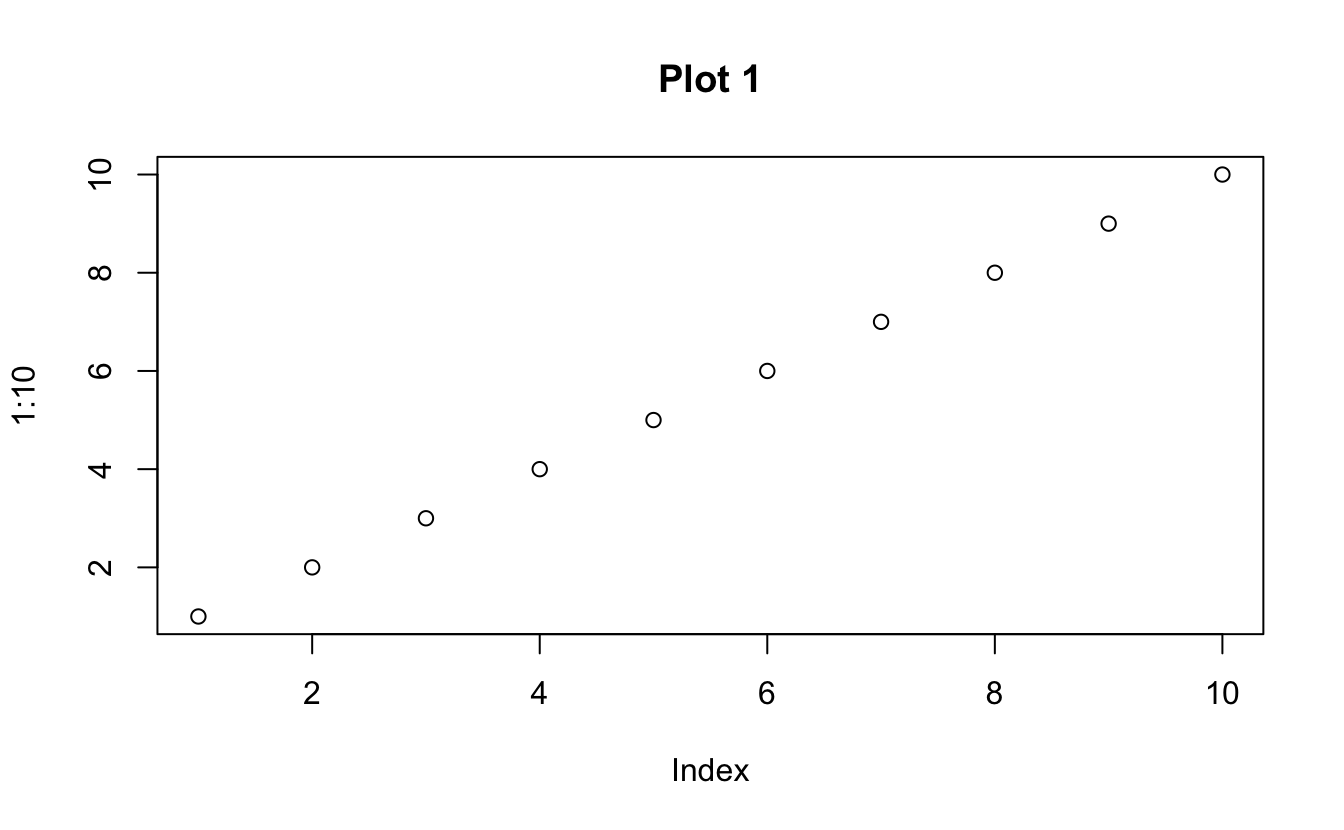
\includegraphics[width=1\linewidth]{mastering-r-through-errors_files/figure-latex/unnamed-chunk-884-1} 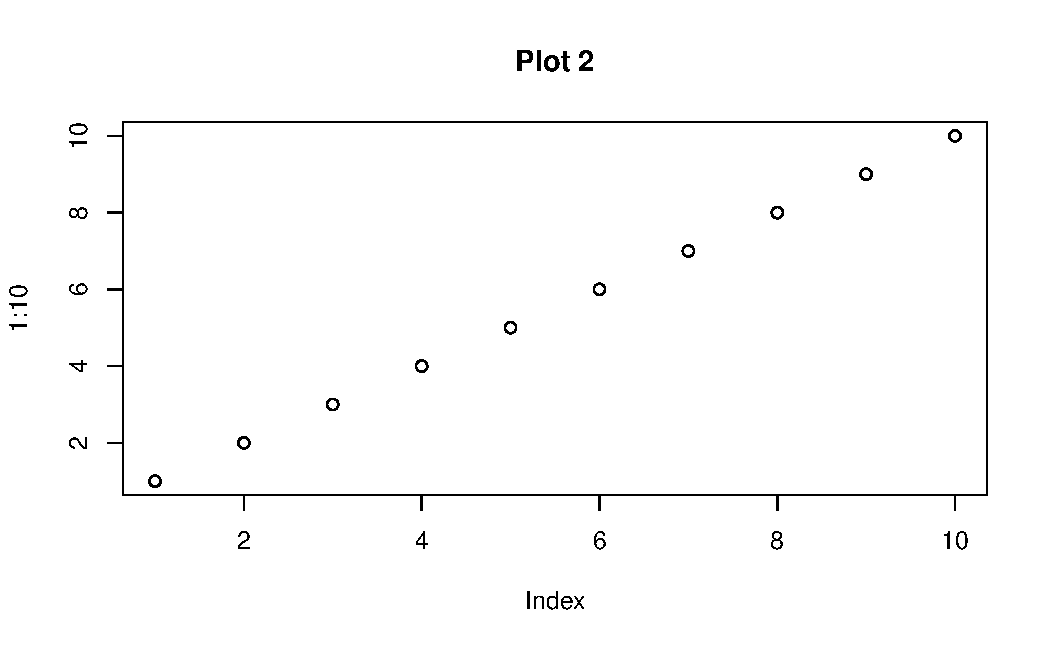
\includegraphics[width=1\linewidth]{mastering-r-through-errors_files/figure-latex/unnamed-chunk-884-2} 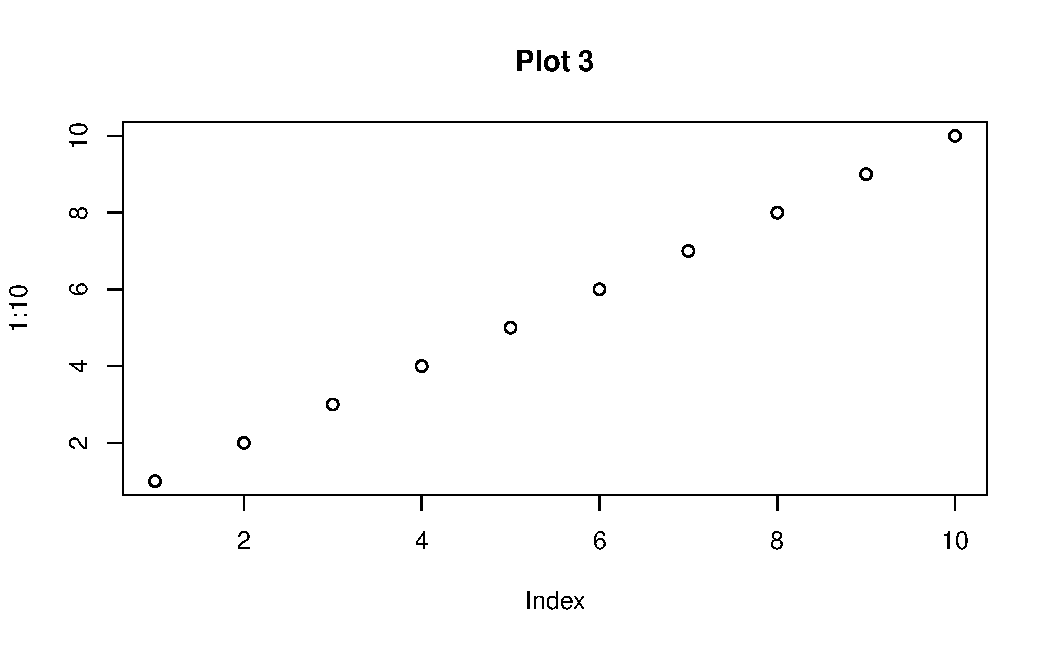
\includegraphics[width=1\linewidth]{mastering-r-through-errors_files/figure-latex/unnamed-chunk-884-3} \end{center}

\section{ifelse() Details}\label{ifelse-details}

💡 \textbf{Key Insight: ifelse() Behavior}

\begin{Shaded}
\begin{Highlighting}[]
\CommentTok{\# Basic ifelse}
\NormalTok{x }\OtherTok{\textless{}{-}} \FunctionTok{c}\NormalTok{(}\DecValTok{1}\NormalTok{, }\DecValTok{5}\NormalTok{, }\DecValTok{3}\NormalTok{, }\DecValTok{8}\NormalTok{, }\DecValTok{2}\NormalTok{)}
\FunctionTok{ifelse}\NormalTok{(x }\SpecialCharTok{\textgreater{}} \DecValTok{4}\NormalTok{, }\StringTok{"High"}\NormalTok{, }\StringTok{"Low"}\NormalTok{)}
\CommentTok{\#\textgreater{} [1] "Low"  "High" "Low"  "High" "Low"}

\CommentTok{\# Nested ifelse}
\FunctionTok{ifelse}\NormalTok{(x }\SpecialCharTok{\textless{}} \DecValTok{3}\NormalTok{, }\StringTok{"Low"}\NormalTok{,}
       \FunctionTok{ifelse}\NormalTok{(x }\SpecialCharTok{\textless{}} \DecValTok{7}\NormalTok{, }\StringTok{"Medium"}\NormalTok{, }\StringTok{"High"}\NormalTok{))}
\CommentTok{\#\textgreater{} [1] "Low"    "Medium" "Medium" "High"   "Low"}

\CommentTok{\# With NAs}
\NormalTok{x\_na }\OtherTok{\textless{}{-}} \FunctionTok{c}\NormalTok{(}\DecValTok{1}\NormalTok{, }\DecValTok{5}\NormalTok{, }\ConstantTok{NA}\NormalTok{, }\DecValTok{8}\NormalTok{, }\DecValTok{2}\NormalTok{)}
\FunctionTok{ifelse}\NormalTok{(x\_na }\SpecialCharTok{\textgreater{}} \DecValTok{4}\NormalTok{, }\StringTok{"High"}\NormalTok{, }\StringTok{"Low"}\NormalTok{)  }\CommentTok{\# NA stays NA}
\CommentTok{\#\textgreater{} [1] "Low"  "High" NA     "High" "Low"}

\CommentTok{\# Type coercion in ifelse}
\FunctionTok{ifelse}\NormalTok{(}\FunctionTok{c}\NormalTok{(}\ConstantTok{TRUE}\NormalTok{, }\ConstantTok{FALSE}\NormalTok{, }\ConstantTok{TRUE}\NormalTok{), }\DecValTok{1}\NormalTok{, }\StringTok{"No"}\NormalTok{)  }\CommentTok{\# Coerces to character!}
\CommentTok{\#\textgreater{} [1] "1"  "No" "1"}

\CommentTok{\# More control with dplyr::case\_when}
\FunctionTok{library}\NormalTok{(dplyr)}
\FunctionTok{case\_when}\NormalTok{(}
\NormalTok{  x }\SpecialCharTok{\textless{}} \DecValTok{3} \SpecialCharTok{\textasciitilde{}} \StringTok{"Low"}\NormalTok{,}
\NormalTok{  x }\SpecialCharTok{\textless{}} \DecValTok{7} \SpecialCharTok{\textasciitilde{}} \StringTok{"Medium"}\NormalTok{,}
  \ConstantTok{TRUE} \SpecialCharTok{\textasciitilde{}} \StringTok{"High"}  \CommentTok{\# Default}
\NormalTok{)}
\CommentTok{\#\textgreater{} [1] "Low"    "Medium" "Medium" "High"   "Low"}

\CommentTok{\# Maintains types better}
\FunctionTok{case\_when}\NormalTok{(}
  \FunctionTok{c}\NormalTok{(}\ConstantTok{TRUE}\NormalTok{, }\ConstantTok{FALSE}\NormalTok{, }\ConstantTok{TRUE}\NormalTok{) }\SpecialCharTok{\textasciitilde{}} \DecValTok{1}\DataTypeTok{L}\NormalTok{,}
  \ConstantTok{TRUE} \SpecialCharTok{\textasciitilde{}} \ConstantTok{NA\_integer\_}
\NormalTok{)}
\CommentTok{\#\textgreater{} [1]  1 NA  1}
\end{Highlighting}
\end{Shaded}

\textbf{Prefer case\_when() for:}
- Multiple conditions
- Type preservation
- Clearer code

\section{Summary}\label{summary-17}

\textbf{Key Takeaways:}

\begin{enumerate}
\def\labelenumi{\arabic{enumi}.}
\tightlist
\item
  \textbf{if needs single logical} - Use \texttt{\&\&}/\texttt{\textbar{}\textbar{}} not \texttt{\&}/\texttt{\textbar{}}
\item
  \textbf{Check length first} - Avoid length-zero errors
\item
  \textbf{Use seq\_along()} - Not \texttt{1:length()} in loops
\item
  \textbf{Pre-allocate vectors} - Important for performance
\item
  \textbf{break exits loop} - \texttt{next} skips iteration
\item
  \textbf{Vectorize when possible} - Usually faster than loops
\item
  \textbf{ifelse() is vectorized} - Different from \texttt{if}
\item
  \textbf{Use case\_when()} - Cleaner than nested ifelse
\end{enumerate}

\textbf{Quick Reference:}

\begin{longtable}[]{@{}
  >{\raggedright\arraybackslash}p{(\linewidth - 4\tabcolsep) * \real{0.3684}}
  >{\raggedright\arraybackslash}p{(\linewidth - 4\tabcolsep) * \real{0.3684}}
  >{\raggedright\arraybackslash}p{(\linewidth - 4\tabcolsep) * \real{0.2632}}@{}}
\toprule\noalign{}
\begin{minipage}[b]{\linewidth}\raggedright
Error
\end{minipage} & \begin{minipage}[b]{\linewidth}\raggedright
Cause
\end{minipage} & \begin{minipage}[b]{\linewidth}\raggedright
Fix
\end{minipage} \\
\midrule\noalign{}
\endhead
\bottomrule\noalign{}
\endlastfoot
condition has length \textgreater{} 1 & Vector in if & Use \texttt{all()}, \texttt{any()}, or \texttt{\&\&}/\texttt{\textbar{}\textbar{}} \\
argument is of length zero & Empty vector in if & Check \texttt{length()} first \\
Infinite loop & No break condition & Add break or fix condition \\
Wrong 1:length() & Empty vector & Use \texttt{seq\_along()} \\
\end{longtable}

\textbf{Control Flow:}

\begin{Shaded}
\begin{Highlighting}[]
\CommentTok{\# if/else}
\ControlFlowTok{if}\NormalTok{ (condition) \{}
  \CommentTok{\# code}
\NormalTok{\} }\ControlFlowTok{else} \ControlFlowTok{if}\NormalTok{ (other\_condition) \{}
  \CommentTok{\# code  }
\NormalTok{\} }\ControlFlowTok{else}\NormalTok{ \{}
  \CommentTok{\# code}
\NormalTok{\}}

\CommentTok{\# ifelse (vectorized)}
\FunctionTok{ifelse}\NormalTok{(test, yes, no)}

\CommentTok{\# for loop}
\ControlFlowTok{for}\NormalTok{ (i }\ControlFlowTok{in} \FunctionTok{seq\_along}\NormalTok{(x)) \{}
  \CommentTok{\# code}
\NormalTok{\}}

\CommentTok{\# while loop}
\ControlFlowTok{while}\NormalTok{ (condition) \{}
  \CommentTok{\# code}
\NormalTok{\}}

\CommentTok{\# repeat loop}
\ControlFlowTok{repeat}\NormalTok{ \{}
  \CommentTok{\# code}
  \ControlFlowTok{if}\NormalTok{ (condition) }\ControlFlowTok{break}
\NormalTok{\}}

\CommentTok{\# switch}
\ControlFlowTok{switch}\NormalTok{(value,}
  \AttributeTok{case1 =}\NormalTok{ result1,}
  \AttributeTok{case2 =}\NormalTok{ result2,}
\NormalTok{  default}
\NormalTok{)}
\end{Highlighting}
\end{Shaded}

\textbf{Best Practices:}

\begin{Shaded}
\begin{Highlighting}[]
\CommentTok{\# ✅ Good}
\ControlFlowTok{if}\NormalTok{ (}\FunctionTok{length}\NormalTok{(x) }\SpecialCharTok{\textgreater{}} \DecValTok{0} \SpecialCharTok{\&\&}\NormalTok{ x[}\DecValTok{1}\NormalTok{] }\SpecialCharTok{\textgreater{}} \DecValTok{5}\NormalTok{)     }\CommentTok{\# Check length}
\ControlFlowTok{for}\NormalTok{ (i }\ControlFlowTok{in} \FunctionTok{seq\_along}\NormalTok{(x))             }\CommentTok{\# Safe indexing}
\NormalTok{result }\OtherTok{\textless{}{-}} \FunctionTok{numeric}\NormalTok{(n); for...       }\CommentTok{\# Pre{-}allocate}
\NormalTok{result }\OtherTok{\textless{}{-}} \FunctionTok{sqrt}\NormalTok{(x)                   }\CommentTok{\# Vectorize when possible}

\CommentTok{\# ❌ Avoid}
\ControlFlowTok{if}\NormalTok{ (x }\SpecialCharTok{\textgreater{}} \DecValTok{5}\NormalTok{)                          }\CommentTok{\# Vector in if}
\ControlFlowTok{for}\NormalTok{ (i }\ControlFlowTok{in} \DecValTok{1}\SpecialCharTok{:}\FunctionTok{length}\NormalTok{(x))              }\CommentTok{\# Fails on empty}
\NormalTok{for... result }\OtherTok{\textless{}{-}} \FunctionTok{c}\NormalTok{(result, new)     }\CommentTok{\# Growing vector (slow)}
\ControlFlowTok{for}\NormalTok{ (i }\ControlFlowTok{in} \DecValTok{1}\SpecialCharTok{:}\NormalTok{n) result[i] }\OtherTok{\textless{}{-}}\NormalTok{ x[i]}\SpecialCharTok{\^{}}\DecValTok{2}  \CommentTok{\# Loop when vectorization works}
\end{Highlighting}
\end{Shaded}

\section{Exercises}\label{exercises-17}

📝 \textbf{Exercise 1: Safe Condition Checker}

Write \texttt{safe\_if(condition,\ true\_val,\ false\_val)} that:
1. Checks if condition is single logical
2. Handles NA in condition
3. Returns appropriate value
4. Gives helpful errors

📝 \textbf{Exercise 2: Loop Converter}

Convert this loop to vectorized code:

\begin{Shaded}
\begin{Highlighting}[]
\NormalTok{x }\OtherTok{\textless{}{-}} \DecValTok{1}\SpecialCharTok{:}\DecValTok{1000}
\NormalTok{result }\OtherTok{\textless{}{-}} \FunctionTok{numeric}\NormalTok{(}\FunctionTok{length}\NormalTok{(x))}
\ControlFlowTok{for}\NormalTok{ (i }\ControlFlowTok{in} \FunctionTok{seq\_along}\NormalTok{(x)) \{}
  \ControlFlowTok{if}\NormalTok{ (x[i] }\SpecialCharTok{\%\%} \DecValTok{2} \SpecialCharTok{==} \DecValTok{0}\NormalTok{) \{}
\NormalTok{    result[i] }\OtherTok{\textless{}{-}}\NormalTok{ x[i]}\SpecialCharTok{\^{}}\DecValTok{2}
\NormalTok{  \} }\ControlFlowTok{else}\NormalTok{ \{}
\NormalTok{    result[i] }\OtherTok{\textless{}{-}}\NormalTok{ x[i]}\SpecialCharTok{\^{}}\DecValTok{3}
\NormalTok{  \}}
\NormalTok{\}}
\end{Highlighting}
\end{Shaded}

📝 \textbf{Exercise 3: Find First}

Write \texttt{find\_first(x,\ condition)} that:
1. Finds first element satisfying condition
2. Returns index and value
3. Handles case where none match
4. Uses early exit for efficiency

📝 \textbf{Exercise 4: Grade Classifier}

Write \texttt{classify\_grade(score)} using switch() that:
1. Converts numeric score to letter grade
2. Handles vectorized input
3. Validates input range (0-100)
4. Returns appropriate grade

\section{Exercise Answers}\label{exercise-answers-17}

Click to see answers

\textbf{Exercise 1:}

\begin{Shaded}
\begin{Highlighting}[]
\NormalTok{safe\_if }\OtherTok{\textless{}{-}} \ControlFlowTok{function}\NormalTok{(condition, true\_val, false\_val) \{}
  \CommentTok{\# Check if condition is logical}
  \ControlFlowTok{if}\NormalTok{ (}\SpecialCharTok{!}\FunctionTok{is.logical}\NormalTok{(condition)) \{}
    \FunctionTok{stop}\NormalTok{(}\StringTok{"Condition must be logical, got "}\NormalTok{, }\FunctionTok{class}\NormalTok{(condition)[}\DecValTok{1}\NormalTok{])}
\NormalTok{  \}}
  
  \CommentTok{\# Check length}
  \ControlFlowTok{if}\NormalTok{ (}\FunctionTok{length}\NormalTok{(condition) }\SpecialCharTok{==} \DecValTok{0}\NormalTok{) \{}
    \FunctionTok{stop}\NormalTok{(}\StringTok{"Condition has length zero"}\NormalTok{)}
\NormalTok{  \}}
  
  \ControlFlowTok{if}\NormalTok{ (}\FunctionTok{length}\NormalTok{(condition) }\SpecialCharTok{\textgreater{}} \DecValTok{1}\NormalTok{) \{}
    \FunctionTok{warning}\NormalTok{(}\StringTok{"Condition has length "}\NormalTok{, }\FunctionTok{length}\NormalTok{(condition), }
            \StringTok{", using first element only"}\NormalTok{)}
\NormalTok{    condition }\OtherTok{\textless{}{-}}\NormalTok{ condition[}\DecValTok{1}\NormalTok{]}
\NormalTok{  \}}
  
  \CommentTok{\# Handle NA}
  \ControlFlowTok{if}\NormalTok{ (}\FunctionTok{is.na}\NormalTok{(condition)) \{}
    \FunctionTok{warning}\NormalTok{(}\StringTok{"Condition is NA, returning NA"}\NormalTok{)}
    \FunctionTok{return}\NormalTok{(}\ConstantTok{NA}\NormalTok{)}
\NormalTok{  \}}
  
  \CommentTok{\# Return appropriate value}
  \ControlFlowTok{if}\NormalTok{ (condition) \{}
\NormalTok{    true\_val}
\NormalTok{  \} }\ControlFlowTok{else}\NormalTok{ \{}
\NormalTok{    false\_val}
\NormalTok{  \}}
\NormalTok{\}}

\CommentTok{\# Test}
\FunctionTok{safe\_if}\NormalTok{(}\ConstantTok{TRUE}\NormalTok{, }\StringTok{"yes"}\NormalTok{, }\StringTok{"no"}\NormalTok{)}
\CommentTok{\#\textgreater{} [1] "yes"}
\FunctionTok{safe\_if}\NormalTok{(}\DecValTok{5} \SpecialCharTok{\textgreater{}} \DecValTok{3}\NormalTok{, }\StringTok{"greater"}\NormalTok{, }\StringTok{"less"}\NormalTok{)}
\CommentTok{\#\textgreater{} [1] "greater"}
\FunctionTok{safe\_if}\NormalTok{(}\ConstantTok{NA}\NormalTok{, }\StringTok{"yes"}\NormalTok{, }\StringTok{"no"}\NormalTok{)  }\CommentTok{\# Warning}
\CommentTok{\#\textgreater{} Warning in safe\_if(NA, "yes", "no"): Condition is NA, returning NA}
\CommentTok{\#\textgreater{} [1] NA}
\FunctionTok{safe\_if}\NormalTok{(}\FunctionTok{c}\NormalTok{(}\ConstantTok{TRUE}\NormalTok{, }\ConstantTok{FALSE}\NormalTok{), }\StringTok{"yes"}\NormalTok{, }\StringTok{"no"}\NormalTok{)  }\CommentTok{\# Warning}
\CommentTok{\#\textgreater{} Warning in safe\_if(c(TRUE, FALSE), "yes", "no"): Condition has length 2, using}
\CommentTok{\#\textgreater{} first element only}
\CommentTok{\#\textgreater{} [1] "yes"}
\end{Highlighting}
\end{Shaded}

\begin{Shaded}
\begin{Highlighting}[]
\FunctionTok{safe\_if}\NormalTok{(}\StringTok{"not logical"}\NormalTok{, }\StringTok{"yes"}\NormalTok{, }\StringTok{"no"}\NormalTok{)  }\CommentTok{\# Error}
\CommentTok{\#\textgreater{} Error in safe\_if("not logical", "yes", "no"): Condition must be logical, got character}
\end{Highlighting}
\end{Shaded}

\textbf{Exercise 2:}

\begin{Shaded}
\begin{Highlighting}[]
\CommentTok{\# Original loop}
\NormalTok{x }\OtherTok{\textless{}{-}} \DecValTok{1}\SpecialCharTok{:}\DecValTok{1000}
\NormalTok{result\_loop }\OtherTok{\textless{}{-}} \FunctionTok{numeric}\NormalTok{(}\FunctionTok{length}\NormalTok{(x))}
\ControlFlowTok{for}\NormalTok{ (i }\ControlFlowTok{in} \FunctionTok{seq\_along}\NormalTok{(x)) \{}
  \ControlFlowTok{if}\NormalTok{ (x[i] }\SpecialCharTok{\%\%} \DecValTok{2} \SpecialCharTok{==} \DecValTok{0}\NormalTok{) \{}
\NormalTok{    result\_loop[i] }\OtherTok{\textless{}{-}}\NormalTok{ x[i]}\SpecialCharTok{\^{}}\DecValTok{2}
\NormalTok{  \} }\ControlFlowTok{else}\NormalTok{ \{}
\NormalTok{    result\_loop[i] }\OtherTok{\textless{}{-}}\NormalTok{ x[i]}\SpecialCharTok{\^{}}\DecValTok{3}
\NormalTok{  \}}
\NormalTok{\}}

\CommentTok{\# Vectorized version 1: ifelse}
\NormalTok{result\_vec1 }\OtherTok{\textless{}{-}} \FunctionTok{ifelse}\NormalTok{(x }\SpecialCharTok{\%\%} \DecValTok{2} \SpecialCharTok{==} \DecValTok{0}\NormalTok{, x}\SpecialCharTok{\^{}}\DecValTok{2}\NormalTok{, x}\SpecialCharTok{\^{}}\DecValTok{3}\NormalTok{)}

\CommentTok{\# Vectorized version 2: case\_when}
\FunctionTok{library}\NormalTok{(dplyr)}
\NormalTok{result\_vec2 }\OtherTok{\textless{}{-}} \FunctionTok{case\_when}\NormalTok{(}
\NormalTok{  x }\SpecialCharTok{\%\%} \DecValTok{2} \SpecialCharTok{==} \DecValTok{0} \SpecialCharTok{\textasciitilde{}}\NormalTok{ x}\SpecialCharTok{\^{}}\DecValTok{2}\NormalTok{,}
  \ConstantTok{TRUE} \SpecialCharTok{\textasciitilde{}}\NormalTok{ x}\SpecialCharTok{\^{}}\DecValTok{3}
\NormalTok{)}

\CommentTok{\# Vectorized version 3: logical indexing}
\NormalTok{result\_vec3 }\OtherTok{\textless{}{-}} \FunctionTok{numeric}\NormalTok{(}\FunctionTok{length}\NormalTok{(x))}
\NormalTok{even }\OtherTok{\textless{}{-}}\NormalTok{ x }\SpecialCharTok{\%\%} \DecValTok{2} \SpecialCharTok{==} \DecValTok{0}
\NormalTok{result\_vec3[even] }\OtherTok{\textless{}{-}}\NormalTok{ x[even]}\SpecialCharTok{\^{}}\DecValTok{2}
\NormalTok{result\_vec3[}\SpecialCharTok{!}\NormalTok{even] }\OtherTok{\textless{}{-}}\NormalTok{ x[}\SpecialCharTok{!}\NormalTok{even]}\SpecialCharTok{\^{}}\DecValTok{3}

\CommentTok{\# Verify all give same result}
\FunctionTok{all.equal}\NormalTok{(result\_loop, result\_vec1)}
\CommentTok{\#\textgreater{} [1] TRUE}
\FunctionTok{all.equal}\NormalTok{(result\_loop, result\_vec2)}
\CommentTok{\#\textgreater{} [1] TRUE}
\FunctionTok{all.equal}\NormalTok{(result\_loop, result\_vec3)}
\CommentTok{\#\textgreater{} [1] TRUE}

\CommentTok{\# Compare performance}
\FunctionTok{library}\NormalTok{(microbenchmark)}
\FunctionTok{microbenchmark}\NormalTok{(}
  \AttributeTok{loop =}\NormalTok{ \{}
\NormalTok{    result }\OtherTok{\textless{}{-}} \FunctionTok{numeric}\NormalTok{(}\FunctionTok{length}\NormalTok{(x))}
    \ControlFlowTok{for}\NormalTok{ (i }\ControlFlowTok{in} \FunctionTok{seq\_along}\NormalTok{(x)) \{}
      \ControlFlowTok{if}\NormalTok{ (x[i] }\SpecialCharTok{\%\%} \DecValTok{2} \SpecialCharTok{==} \DecValTok{0}\NormalTok{) result[i] }\OtherTok{\textless{}{-}}\NormalTok{ x[i]}\SpecialCharTok{\^{}}\DecValTok{2}
      \ControlFlowTok{else}\NormalTok{ result[i] }\OtherTok{\textless{}{-}}\NormalTok{ x[i]}\SpecialCharTok{\^{}}\DecValTok{3}
\NormalTok{    \}}
\NormalTok{  \},}
  \AttributeTok{ifelse =} \FunctionTok{ifelse}\NormalTok{(x }\SpecialCharTok{\%\%} \DecValTok{2} \SpecialCharTok{==} \DecValTok{0}\NormalTok{, x}\SpecialCharTok{\^{}}\DecValTok{2}\NormalTok{, x}\SpecialCharTok{\^{}}\DecValTok{3}\NormalTok{),}
  \AttributeTok{case\_when =} \FunctionTok{case\_when}\NormalTok{(x }\SpecialCharTok{\%\%} \DecValTok{2} \SpecialCharTok{==} \DecValTok{0} \SpecialCharTok{\textasciitilde{}}\NormalTok{ x}\SpecialCharTok{\^{}}\DecValTok{2}\NormalTok{, }\ConstantTok{TRUE} \SpecialCharTok{\textasciitilde{}}\NormalTok{ x}\SpecialCharTok{\^{}}\DecValTok{3}\NormalTok{),}
  \AttributeTok{logical\_index =}\NormalTok{ \{}
\NormalTok{    result }\OtherTok{\textless{}{-}} \FunctionTok{numeric}\NormalTok{(}\FunctionTok{length}\NormalTok{(x))}
\NormalTok{    even }\OtherTok{\textless{}{-}}\NormalTok{ x }\SpecialCharTok{\%\%} \DecValTok{2} \SpecialCharTok{==} \DecValTok{0}
\NormalTok{    result[even] }\OtherTok{\textless{}{-}}\NormalTok{ x[even]}\SpecialCharTok{\^{}}\DecValTok{2}
\NormalTok{    result[}\SpecialCharTok{!}\NormalTok{even] }\OtherTok{\textless{}{-}}\NormalTok{ x[}\SpecialCharTok{!}\NormalTok{even]}\SpecialCharTok{\^{}}\DecValTok{3}
\NormalTok{  \},}
  \AttributeTok{times =} \DecValTok{100}
\NormalTok{)}
\CommentTok{\#\textgreater{} Unit: microseconds}
\CommentTok{\#\textgreater{}           expr      min        lq       mean    median        uq       max}
\CommentTok{\#\textgreater{}           loop 4405.050 5216.8515 5951.63854 5524.5045 5806.1620 30718.845}
\CommentTok{\#\textgreater{}         ifelse   50.257   53.7865   63.76264   59.9795   66.7645   153.114}
\CommentTok{\#\textgreater{}      case\_when  231.696  277.7470  376.20880  370.8985  445.6850   997.188}
\CommentTok{\#\textgreater{}  logical\_index   37.715   40.8840   49.52790   46.1855   50.6055   237.059}
\CommentTok{\#\textgreater{}  neval}
\CommentTok{\#\textgreater{}    100}
\CommentTok{\#\textgreater{}    100}
\CommentTok{\#\textgreater{}    100}
\CommentTok{\#\textgreater{}    100}
\end{Highlighting}
\end{Shaded}

\textbf{Exercise 3:}

\begin{Shaded}
\begin{Highlighting}[]
\NormalTok{find\_first }\OtherTok{\textless{}{-}} \ControlFlowTok{function}\NormalTok{(x, condition) \{}
  \CommentTok{\# Validate inputs}
  \ControlFlowTok{if}\NormalTok{ (}\SpecialCharTok{!}\FunctionTok{is.function}\NormalTok{(condition)) \{}
    \FunctionTok{stop}\NormalTok{(}\StringTok{"condition must be a function"}\NormalTok{)}
\NormalTok{  \}}
  
  \ControlFlowTok{if}\NormalTok{ (}\FunctionTok{length}\NormalTok{(x) }\SpecialCharTok{==} \DecValTok{0}\NormalTok{) \{}
    \FunctionTok{return}\NormalTok{(}\FunctionTok{list}\NormalTok{(}\AttributeTok{index =} \ConstantTok{NA}\NormalTok{, }\AttributeTok{value =} \ConstantTok{NA}\NormalTok{, }\AttributeTok{found =} \ConstantTok{FALSE}\NormalTok{))}
\NormalTok{  \}}
  
  \CommentTok{\# Search with early exit}
  \ControlFlowTok{for}\NormalTok{ (i }\ControlFlowTok{in} \FunctionTok{seq\_along}\NormalTok{(x)) \{}
    \ControlFlowTok{if}\NormalTok{ (}\FunctionTok{condition}\NormalTok{(x[i])) \{}
      \FunctionTok{return}\NormalTok{(}\FunctionTok{list}\NormalTok{(}
        \AttributeTok{index =}\NormalTok{ i,}
        \AttributeTok{value =}\NormalTok{ x[i],}
        \AttributeTok{found =} \ConstantTok{TRUE}
\NormalTok{      ))}
\NormalTok{    \}}
\NormalTok{  \}}
  
  \CommentTok{\# None found}
  \FunctionTok{list}\NormalTok{(}\AttributeTok{index =} \ConstantTok{NA}\NormalTok{, }\AttributeTok{value =} \ConstantTok{NA}\NormalTok{, }\AttributeTok{found =} \ConstantTok{FALSE}\NormalTok{)}
\NormalTok{\}}

\CommentTok{\# Test}
\NormalTok{data }\OtherTok{\textless{}{-}} \FunctionTok{c}\NormalTok{(}\DecValTok{1}\NormalTok{, }\DecValTok{3}\NormalTok{, }\DecValTok{5}\NormalTok{, }\DecValTok{8}\NormalTok{, }\DecValTok{2}\NormalTok{, }\DecValTok{9}\NormalTok{, }\DecValTok{4}\NormalTok{)}

\CommentTok{\# Find first \textgreater{} 5}
\FunctionTok{find\_first}\NormalTok{(data, }\ControlFlowTok{function}\NormalTok{(x) x }\SpecialCharTok{\textgreater{}} \DecValTok{5}\NormalTok{)}
\CommentTok{\#\textgreater{} $index}
\CommentTok{\#\textgreater{} [1] 4}
\CommentTok{\#\textgreater{} }
\CommentTok{\#\textgreater{} $value}
\CommentTok{\#\textgreater{} [1] 8}
\CommentTok{\#\textgreater{} }
\CommentTok{\#\textgreater{} $found}
\CommentTok{\#\textgreater{} [1] TRUE}

\CommentTok{\# Find first even}
\FunctionTok{find\_first}\NormalTok{(data, }\ControlFlowTok{function}\NormalTok{(x) x }\SpecialCharTok{\%\%} \DecValTok{2} \SpecialCharTok{==} \DecValTok{0}\NormalTok{)}
\CommentTok{\#\textgreater{} $index}
\CommentTok{\#\textgreater{} [1] 4}
\CommentTok{\#\textgreater{} }
\CommentTok{\#\textgreater{} $value}
\CommentTok{\#\textgreater{} [1] 8}
\CommentTok{\#\textgreater{} }
\CommentTok{\#\textgreater{} $found}
\CommentTok{\#\textgreater{} [1] TRUE}

\CommentTok{\# Find first \textgreater{} 100 (none)}
\FunctionTok{find\_first}\NormalTok{(data, }\ControlFlowTok{function}\NormalTok{(x) x }\SpecialCharTok{\textgreater{}} \DecValTok{100}\NormalTok{)}
\CommentTok{\#\textgreater{} $index}
\CommentTok{\#\textgreater{} [1] NA}
\CommentTok{\#\textgreater{} }
\CommentTok{\#\textgreater{} $value}
\CommentTok{\#\textgreater{} [1] NA}
\CommentTok{\#\textgreater{} }
\CommentTok{\#\textgreater{} $found}
\CommentTok{\#\textgreater{} [1] FALSE}

\CommentTok{\# Empty vector}
\FunctionTok{find\_first}\NormalTok{(}\FunctionTok{numeric}\NormalTok{(}\DecValTok{0}\NormalTok{), }\ControlFlowTok{function}\NormalTok{(x) x }\SpecialCharTok{\textgreater{}} \DecValTok{5}\NormalTok{)}
\CommentTok{\#\textgreater{} $index}
\CommentTok{\#\textgreater{} [1] NA}
\CommentTok{\#\textgreater{} }
\CommentTok{\#\textgreater{} $value}
\CommentTok{\#\textgreater{} [1] NA}
\CommentTok{\#\textgreater{} }
\CommentTok{\#\textgreater{} $found}
\CommentTok{\#\textgreater{} [1] FALSE}

\CommentTok{\# More complex condition}
\FunctionTok{find\_first}\NormalTok{(}\FunctionTok{c}\NormalTok{(}\StringTok{"apple"}\NormalTok{, }\StringTok{"banana"}\NormalTok{, }\StringTok{"cherry"}\NormalTok{), }
          \ControlFlowTok{function}\NormalTok{(x) }\FunctionTok{nchar}\NormalTok{(x) }\SpecialCharTok{\textgreater{}} \DecValTok{5}\NormalTok{)}
\CommentTok{\#\textgreater{} $index}
\CommentTok{\#\textgreater{} [1] 2}
\CommentTok{\#\textgreater{} }
\CommentTok{\#\textgreater{} $value}
\CommentTok{\#\textgreater{} [1] "banana"}
\CommentTok{\#\textgreater{} }
\CommentTok{\#\textgreater{} $found}
\CommentTok{\#\textgreater{} [1] TRUE}
\end{Highlighting}
\end{Shaded}

\textbf{Exercise 4:}

\begin{Shaded}
\begin{Highlighting}[]
\NormalTok{classify\_grade }\OtherTok{\textless{}{-}} \ControlFlowTok{function}\NormalTok{(score) \{}
  \CommentTok{\# Validate input}
  \ControlFlowTok{if}\NormalTok{ (}\SpecialCharTok{!}\FunctionTok{is.numeric}\NormalTok{(score)) \{}
    \FunctionTok{stop}\NormalTok{(}\StringTok{"Score must be numeric"}\NormalTok{)}
\NormalTok{  \}}
  
  \CommentTok{\# Vectorized function}
  \FunctionTok{sapply}\NormalTok{(score, }\ControlFlowTok{function}\NormalTok{(s) \{}
    \CommentTok{\# Check range}
    \ControlFlowTok{if}\NormalTok{ (}\FunctionTok{is.na}\NormalTok{(s)) \{}
      \FunctionTok{return}\NormalTok{(}\ConstantTok{NA\_character\_}\NormalTok{)}
\NormalTok{    \}}
    
    \ControlFlowTok{if}\NormalTok{ (s }\SpecialCharTok{\textless{}} \DecValTok{0} \SpecialCharTok{||}\NormalTok{ s }\SpecialCharTok{\textgreater{}} \DecValTok{100}\NormalTok{) \{}
      \FunctionTok{warning}\NormalTok{(}\StringTok{"Score "}\NormalTok{, s, }\StringTok{" is out of range (0{-}100)"}\NormalTok{)}
      \FunctionTok{return}\NormalTok{(}\StringTok{"Invalid"}\NormalTok{)}
\NormalTok{    \}}
    
    \CommentTok{\# Classify using switch on integer ranges}
\NormalTok{    grade\_num }\OtherTok{\textless{}{-}} \FunctionTok{cut}\NormalTok{(s, }
                    \AttributeTok{breaks =} \FunctionTok{c}\NormalTok{(}\SpecialCharTok{{-}}\ConstantTok{Inf}\NormalTok{, }\DecValTok{60}\NormalTok{, }\DecValTok{70}\NormalTok{, }\DecValTok{80}\NormalTok{, }\DecValTok{90}\NormalTok{, }\ConstantTok{Inf}\NormalTok{),}
                    \AttributeTok{labels =} \ConstantTok{FALSE}\NormalTok{)}
    
    \ControlFlowTok{switch}\NormalTok{(grade\_num,}
      \StringTok{"F"}\NormalTok{,  }\CommentTok{\# 1: 0{-}59}
      \StringTok{"D"}\NormalTok{,  }\CommentTok{\# 2: 60{-}69}
      \StringTok{"C"}\NormalTok{,  }\CommentTok{\# 3: 70{-}79}
      \StringTok{"B"}\NormalTok{,  }\CommentTok{\# 4: 80{-}89}
      \StringTok{"A"}   \CommentTok{\# 5: 90{-}100}
\NormalTok{    )}
\NormalTok{  \})}
\NormalTok{\}}

\CommentTok{\# Test}
\FunctionTok{classify\_grade}\NormalTok{(}\DecValTok{85}\NormalTok{)}
\CommentTok{\#\textgreater{} [1] "B"}
\FunctionTok{classify\_grade}\NormalTok{(}\FunctionTok{c}\NormalTok{(}\DecValTok{45}\NormalTok{, }\DecValTok{65}\NormalTok{, }\DecValTok{75}\NormalTok{, }\DecValTok{85}\NormalTok{, }\DecValTok{95}\NormalTok{))}
\CommentTok{\#\textgreater{} [1] "F" "D" "C" "B" "A"}
\FunctionTok{classify\_grade}\NormalTok{(}\FunctionTok{c}\NormalTok{(}\DecValTok{95}\NormalTok{, }\ConstantTok{NA}\NormalTok{, }\DecValTok{105}\NormalTok{, }\DecValTok{65}\NormalTok{))}
\CommentTok{\#\textgreater{} Warning in FUN(X[[i]], ...): Score 105 is out of range (0{-}100)}
\CommentTok{\#\textgreater{} [1] "A"       NA        "Invalid" "D"}

\CommentTok{\# More detailed version with +/{-}}
\NormalTok{classify\_grade\_detailed }\OtherTok{\textless{}{-}} \ControlFlowTok{function}\NormalTok{(score) \{}
  \FunctionTok{sapply}\NormalTok{(score, }\ControlFlowTok{function}\NormalTok{(s) \{}
    \ControlFlowTok{if}\NormalTok{ (}\FunctionTok{is.na}\NormalTok{(s)) }\FunctionTok{return}\NormalTok{(}\ConstantTok{NA\_character\_}\NormalTok{)}
    \ControlFlowTok{if}\NormalTok{ (s }\SpecialCharTok{\textless{}} \DecValTok{0} \SpecialCharTok{||}\NormalTok{ s }\SpecialCharTok{\textgreater{}} \DecValTok{100}\NormalTok{) }\FunctionTok{return}\NormalTok{(}\StringTok{"Invalid"}\NormalTok{)}
    
    \ControlFlowTok{if}\NormalTok{ (s }\SpecialCharTok{\textgreater{}=} \DecValTok{97}\NormalTok{) }\FunctionTok{return}\NormalTok{(}\StringTok{"A+"}\NormalTok{)}
    \ControlFlowTok{if}\NormalTok{ (s }\SpecialCharTok{\textgreater{}=} \DecValTok{93}\NormalTok{) }\FunctionTok{return}\NormalTok{(}\StringTok{"A"}\NormalTok{)}
    \ControlFlowTok{if}\NormalTok{ (s }\SpecialCharTok{\textgreater{}=} \DecValTok{90}\NormalTok{) }\FunctionTok{return}\NormalTok{(}\StringTok{"A{-}"}\NormalTok{)}
    \ControlFlowTok{if}\NormalTok{ (s }\SpecialCharTok{\textgreater{}=} \DecValTok{87}\NormalTok{) }\FunctionTok{return}\NormalTok{(}\StringTok{"B+"}\NormalTok{)}
    \ControlFlowTok{if}\NormalTok{ (s }\SpecialCharTok{\textgreater{}=} \DecValTok{83}\NormalTok{) }\FunctionTok{return}\NormalTok{(}\StringTok{"B"}\NormalTok{)}
    \ControlFlowTok{if}\NormalTok{ (s }\SpecialCharTok{\textgreater{}=} \DecValTok{80}\NormalTok{) }\FunctionTok{return}\NormalTok{(}\StringTok{"B{-}"}\NormalTok{)}
    \ControlFlowTok{if}\NormalTok{ (s }\SpecialCharTok{\textgreater{}=} \DecValTok{77}\NormalTok{) }\FunctionTok{return}\NormalTok{(}\StringTok{"C+"}\NormalTok{)}
    \ControlFlowTok{if}\NormalTok{ (s }\SpecialCharTok{\textgreater{}=} \DecValTok{73}\NormalTok{) }\FunctionTok{return}\NormalTok{(}\StringTok{"C"}\NormalTok{)}
    \ControlFlowTok{if}\NormalTok{ (s }\SpecialCharTok{\textgreater{}=} \DecValTok{70}\NormalTok{) }\FunctionTok{return}\NormalTok{(}\StringTok{"C{-}"}\NormalTok{)}
    \ControlFlowTok{if}\NormalTok{ (s }\SpecialCharTok{\textgreater{}=} \DecValTok{67}\NormalTok{) }\FunctionTok{return}\NormalTok{(}\StringTok{"D+"}\NormalTok{)}
    \ControlFlowTok{if}\NormalTok{ (s }\SpecialCharTok{\textgreater{}=} \DecValTok{63}\NormalTok{) }\FunctionTok{return}\NormalTok{(}\StringTok{"D"}\NormalTok{)}
    \ControlFlowTok{if}\NormalTok{ (s }\SpecialCharTok{\textgreater{}=} \DecValTok{60}\NormalTok{) }\FunctionTok{return}\NormalTok{(}\StringTok{"D{-}"}\NormalTok{)}
    \FunctionTok{return}\NormalTok{(}\StringTok{"F"}\NormalTok{)}
\NormalTok{  \})}
\NormalTok{\}}

\FunctionTok{classify\_grade\_detailed}\NormalTok{(}\FunctionTok{c}\NormalTok{(}\DecValTok{98}\NormalTok{, }\DecValTok{88}\NormalTok{, }\DecValTok{78}\NormalTok{, }\DecValTok{68}\NormalTok{, }\DecValTok{58}\NormalTok{))}
\CommentTok{\#\textgreater{} [1] "A+" "B+" "C+" "D+" "F"}
\end{Highlighting}
\end{Shaded}

\chapter{Error Handling}\label{error-handling}

\textbf{What You'll Learn:}

\begin{itemize}
\tightlist
\item
  try() and tryCatch()
\item
  Creating custom errors
\item
  Warning and message handling
\item
  Defensive programming
\item
  Debugging strategies
\end{itemize}

\textbf{Key Errors Covered:} 12+ error handling patterns

\textbf{Difficulty:} ⭐⭐⭐ Advanced

\section{Introduction}\label{introduction-18}

Error handling lets you gracefully handle problems:

\begin{Shaded}
\begin{Highlighting}[]
\CommentTok{\# Without error handling}
\NormalTok{result }\OtherTok{\textless{}{-}} \FunctionTok{log}\NormalTok{(}\StringTok{"not a number"}\NormalTok{)}
\CommentTok{\#\textgreater{} Error in log("not a number"): non{-}numeric argument to mathematical function}
\end{Highlighting}
\end{Shaded}

\begin{Shaded}
\begin{Highlighting}[]
\CommentTok{\# With error handling}
\NormalTok{result }\OtherTok{\textless{}{-}} \FunctionTok{try}\NormalTok{(}\FunctionTok{log}\NormalTok{(}\StringTok{"not a number"}\NormalTok{), }\AttributeTok{silent =} \ConstantTok{TRUE}\NormalTok{)}

\ControlFlowTok{if}\NormalTok{ (}\FunctionTok{inherits}\NormalTok{(result, }\StringTok{"try{-}error"}\NormalTok{)) \{}
  \FunctionTok{cat}\NormalTok{(}\StringTok{"Error occurred, using default value}\SpecialCharTok{\textbackslash{}n}\StringTok{"}\NormalTok{)}
\NormalTok{  result }\OtherTok{\textless{}{-}} \ConstantTok{NA}
\NormalTok{\}}
\CommentTok{\#\textgreater{} Error occurred, using default value}
\NormalTok{result}
\CommentTok{\#\textgreater{} [1] NA}
\end{Highlighting}
\end{Shaded}

Let's master error handling for robust code.

\section{Error Basics}\label{error-basics}

💡 \textbf{Key Insight: Errors, Warnings, Messages}

\begin{Shaded}
\begin{Highlighting}[]
\CommentTok{\# Error: stops execution}
\FunctionTok{stop}\NormalTok{(}\StringTok{"This is an error"}\NormalTok{)}
\CommentTok{\#\textgreater{} Error: This is an error}
\end{Highlighting}
\end{Shaded}

\begin{Shaded}
\begin{Highlighting}[]
\CommentTok{\# Warning: continues execution}
\FunctionTok{warning}\NormalTok{(}\StringTok{"This is a warning"}\NormalTok{)}
\CommentTok{\#\textgreater{} Warning: This is a warning}
\FunctionTok{cat}\NormalTok{(}\StringTok{"Execution continues}\SpecialCharTok{\textbackslash{}n}\StringTok{"}\NormalTok{)}
\CommentTok{\#\textgreater{} Execution continues}

\CommentTok{\# Message: informational}
\FunctionTok{message}\NormalTok{(}\StringTok{"This is a message"}\NormalTok{)}
\CommentTok{\#\textgreater{} This is a message}
\FunctionTok{cat}\NormalTok{(}\StringTok{"Execution continues}\SpecialCharTok{\textbackslash{}n}\StringTok{"}\NormalTok{)}
\CommentTok{\#\textgreater{} Execution continues}

\CommentTok{\# Creating conditions}
\CommentTok{\# Error}
\NormalTok{error\_func }\OtherTok{\textless{}{-}} \ControlFlowTok{function}\NormalTok{(x) \{}
  \ControlFlowTok{if}\NormalTok{ (x }\SpecialCharTok{\textless{}} \DecValTok{0}\NormalTok{) \{}
    \FunctionTok{stop}\NormalTok{(}\StringTok{"x must be non{-}negative"}\NormalTok{)}
\NormalTok{  \}}
  \FunctionTok{sqrt}\NormalTok{(x)}
\NormalTok{\}}
\end{Highlighting}
\end{Shaded}

\begin{Shaded}
\begin{Highlighting}[]
\FunctionTok{error\_func}\NormalTok{(}\SpecialCharTok{{-}}\DecValTok{5}\NormalTok{)}
\CommentTok{\#\textgreater{} Error in error\_func({-}5): x must be non{-}negative}
\end{Highlighting}
\end{Shaded}

\begin{Shaded}
\begin{Highlighting}[]
\CommentTok{\# Warning}
\NormalTok{warn\_func }\OtherTok{\textless{}{-}} \ControlFlowTok{function}\NormalTok{(x) \{}
  \ControlFlowTok{if}\NormalTok{ (x }\SpecialCharTok{\textless{}} \DecValTok{0}\NormalTok{) \{}
    \FunctionTok{warning}\NormalTok{(}\StringTok{"x is negative, taking absolute value"}\NormalTok{)}
\NormalTok{    x }\OtherTok{\textless{}{-}} \FunctionTok{abs}\NormalTok{(x)}
\NormalTok{  \}}
  \FunctionTok{sqrt}\NormalTok{(x)}
\NormalTok{\}}

\FunctionTok{warn\_func}\NormalTok{(}\SpecialCharTok{{-}}\DecValTok{5}\NormalTok{)}
\CommentTok{\#\textgreater{} Warning in warn\_func({-}5): x is negative, taking absolute value}
\CommentTok{\#\textgreater{} [1] 2.236068}

\CommentTok{\# Message}
\NormalTok{message\_func }\OtherTok{\textless{}{-}} \ControlFlowTok{function}\NormalTok{(x) \{}
  \FunctionTok{message}\NormalTok{(}\StringTok{"Calculating square root of "}\NormalTok{, x)}
  \FunctionTok{sqrt}\NormalTok{(x)}
\NormalTok{\}}

\FunctionTok{message\_func}\NormalTok{(}\DecValTok{25}\NormalTok{)}
\CommentTok{\#\textgreater{} Calculating square root of 25}
\CommentTok{\#\textgreater{} [1] 5}
\end{Highlighting}
\end{Shaded}

\section{try()}\label{try}

💡 \textbf{Key Insight: try() Basics}

\begin{Shaded}
\begin{Highlighting}[]
\CommentTok{\# Without try: error stops everything}
\NormalTok{safe\_log }\OtherTok{\textless{}{-}} \ControlFlowTok{function}\NormalTok{(x) \{}
\NormalTok{  result }\OtherTok{\textless{}{-}} \FunctionTok{try}\NormalTok{(}\FunctionTok{log}\NormalTok{(x), }\AttributeTok{silent =} \ConstantTok{TRUE}\NormalTok{)}
  
  \ControlFlowTok{if}\NormalTok{ (}\FunctionTok{inherits}\NormalTok{(result, }\StringTok{"try{-}error"}\NormalTok{)) \{}
    \FunctionTok{return}\NormalTok{(}\ConstantTok{NA}\NormalTok{)}
\NormalTok{  \}}
  
\NormalTok{  result}
\NormalTok{\}}

\CommentTok{\# Test}
\FunctionTok{safe\_log}\NormalTok{(}\DecValTok{10}\NormalTok{)      }\CommentTok{\# Works}
\CommentTok{\#\textgreater{} [1] 2.302585}
\FunctionTok{safe\_log}\NormalTok{(}\StringTok{"text"}\NormalTok{)  }\CommentTok{\# Returns NA instead of error}
\CommentTok{\#\textgreater{} [1] NA}

\CommentTok{\# Process multiple values}
\NormalTok{values }\OtherTok{\textless{}{-}} \FunctionTok{list}\NormalTok{(}\DecValTok{10}\NormalTok{, }\StringTok{"text"}\NormalTok{, }\DecValTok{100}\NormalTok{, }\StringTok{"more text"}\NormalTok{, }\DecValTok{50}\NormalTok{)}

\NormalTok{results }\OtherTok{\textless{}{-}} \FunctionTok{lapply}\NormalTok{(values, safe\_log)}
\NormalTok{results}
\CommentTok{\#\textgreater{} [[1]]}
\CommentTok{\#\textgreater{} [1] 2.302585}
\CommentTok{\#\textgreater{} }
\CommentTok{\#\textgreater{} [[2]]}
\CommentTok{\#\textgreater{} [1] NA}
\CommentTok{\#\textgreater{} }
\CommentTok{\#\textgreater{} [[3]]}
\CommentTok{\#\textgreater{} [1] 4.60517}
\CommentTok{\#\textgreater{} }
\CommentTok{\#\textgreater{} [[4]]}
\CommentTok{\#\textgreater{} [1] NA}
\CommentTok{\#\textgreater{} }
\CommentTok{\#\textgreater{} [[5]]}
\CommentTok{\#\textgreater{} [1] 3.912023}

\CommentTok{\# Or with verbose errors}
\NormalTok{results\_verbose }\OtherTok{\textless{}{-}} \FunctionTok{lapply}\NormalTok{(values, }\ControlFlowTok{function}\NormalTok{(x) \{}
  \FunctionTok{try}\NormalTok{(}\FunctionTok{log}\NormalTok{(x), }\AttributeTok{silent =} \ConstantTok{FALSE}\NormalTok{)}
\NormalTok{\})}
\CommentTok{\#\textgreater{} Error in log(x) : non{-}numeric argument to mathematical function}
\CommentTok{\#\textgreater{} Error in log(x) : non{-}numeric argument to mathematical function}
\end{Highlighting}
\end{Shaded}

\textbf{When to use try():}
- Simple error catching
- Don't need to distinguish error types
- Want to return special value on error
- Processing multiple items

\section{tryCatch()}\label{trycatch}

💡 \textbf{Key Insight: tryCatch() for Full Control}

\begin{Shaded}
\begin{Highlighting}[]
\CommentTok{\# Full control over errors, warnings, messages}
\NormalTok{safe\_divide }\OtherTok{\textless{}{-}} \ControlFlowTok{function}\NormalTok{(x, y) \{}
  \FunctionTok{tryCatch}\NormalTok{(}
\NormalTok{    \{}
      \CommentTok{\# Try this code}
      \ControlFlowTok{if}\NormalTok{ (y }\SpecialCharTok{==} \DecValTok{0}\NormalTok{) }\FunctionTok{stop}\NormalTok{(}\StringTok{"Division by zero"}\NormalTok{)}
\NormalTok{      x }\SpecialCharTok{/}\NormalTok{ y}
\NormalTok{    \},}
    \AttributeTok{error =} \ControlFlowTok{function}\NormalTok{(e) \{}
      \CommentTok{\# Handle error}
      \FunctionTok{message}\NormalTok{(}\StringTok{"Error: "}\NormalTok{, e}\SpecialCharTok{$}\NormalTok{message)}
      \FunctionTok{return}\NormalTok{(}\ConstantTok{Inf}\NormalTok{)}
\NormalTok{    \},}
    \AttributeTok{warning =} \ControlFlowTok{function}\NormalTok{(w) \{}
      \CommentTok{\# Handle warning}
      \FunctionTok{message}\NormalTok{(}\StringTok{"Warning: "}\NormalTok{, w}\SpecialCharTok{$}\NormalTok{message)}
\NormalTok{    \},}
    \AttributeTok{finally =}\NormalTok{ \{}
      \CommentTok{\# Always runs (cleanup)}
      \FunctionTok{message}\NormalTok{(}\StringTok{"Division attempted"}\NormalTok{)}
\NormalTok{    \}}
\NormalTok{  )}
\NormalTok{\}}

\FunctionTok{safe\_divide}\NormalTok{(}\DecValTok{10}\NormalTok{, }\DecValTok{2}\NormalTok{)}
\CommentTok{\#\textgreater{} Division attempted}
\CommentTok{\#\textgreater{} [1] 5}
\FunctionTok{safe\_divide}\NormalTok{(}\DecValTok{10}\NormalTok{, }\DecValTok{0}\NormalTok{)}
\CommentTok{\#\textgreater{} Error: Division by zero}
\CommentTok{\#\textgreater{} Division attempted}
\CommentTok{\#\textgreater{} [1] Inf}

\CommentTok{\# More complex example}
\NormalTok{read\_data\_safe }\OtherTok{\textless{}{-}} \ControlFlowTok{function}\NormalTok{(file) \{}
  \FunctionTok{tryCatch}\NormalTok{(}
\NormalTok{    \{}
\NormalTok{      data }\OtherTok{\textless{}{-}} \FunctionTok{read.csv}\NormalTok{(file)}
      \FunctionTok{message}\NormalTok{(}\StringTok{"Successfully read "}\NormalTok{, }\FunctionTok{nrow}\NormalTok{(data), }\StringTok{" rows"}\NormalTok{)}
\NormalTok{      data}
\NormalTok{    \},}
    \AttributeTok{error =} \ControlFlowTok{function}\NormalTok{(e) \{}
      \ControlFlowTok{if}\NormalTok{ (}\FunctionTok{grepl}\NormalTok{(}\StringTok{"cannot open"}\NormalTok{, e}\SpecialCharTok{$}\NormalTok{message)) \{}
        \FunctionTok{stop}\NormalTok{(}\StringTok{"File not found: "}\NormalTok{, file)}
\NormalTok{      \} }\ControlFlowTok{else} \ControlFlowTok{if}\NormalTok{ (}\FunctionTok{grepl}\NormalTok{(}\StringTok{"more columns"}\NormalTok{, e}\SpecialCharTok{$}\NormalTok{message)) \{}
        \FunctionTok{stop}\NormalTok{(}\StringTok{"File format error in: "}\NormalTok{, file)}
\NormalTok{      \} }\ControlFlowTok{else}\NormalTok{ \{}
        \FunctionTok{stop}\NormalTok{(}\StringTok{"Unknown error reading: "}\NormalTok{, file, }\StringTok{"}\SpecialCharTok{\textbackslash{}n}\StringTok{"}\NormalTok{, e}\SpecialCharTok{$}\NormalTok{message)}
\NormalTok{      \}}
\NormalTok{    \}}
\NormalTok{  )}
\NormalTok{\}}

\CommentTok{\# Example with warnings}
\NormalTok{sqrt\_checked }\OtherTok{\textless{}{-}} \ControlFlowTok{function}\NormalTok{(x) \{}
  \FunctionTok{tryCatch}\NormalTok{(}
\NormalTok{    \{}
      \ControlFlowTok{if}\NormalTok{ (}\SpecialCharTok{!}\FunctionTok{is.numeric}\NormalTok{(x)) \{}
        \FunctionTok{stop}\NormalTok{(}\StringTok{"Input must be numeric"}\NormalTok{)}
\NormalTok{      \}}
      \ControlFlowTok{if}\NormalTok{ (}\FunctionTok{any}\NormalTok{(x }\SpecialCharTok{\textless{}} \DecValTok{0}\NormalTok{)) \{}
        \FunctionTok{warning}\NormalTok{(}\StringTok{"Negative values detected, taking absolute value"}\NormalTok{)}
\NormalTok{        x }\OtherTok{\textless{}{-}} \FunctionTok{abs}\NormalTok{(x)}
\NormalTok{      \}}
      \FunctionTok{sqrt}\NormalTok{(x)}
\NormalTok{    \},}
    \AttributeTok{error =} \ControlFlowTok{function}\NormalTok{(e) \{}
      \FunctionTok{message}\NormalTok{(}\StringTok{"Error: "}\NormalTok{, e}\SpecialCharTok{$}\NormalTok{message)}
      \FunctionTok{return}\NormalTok{(}\FunctionTok{rep}\NormalTok{(}\ConstantTok{NA}\NormalTok{, }\FunctionTok{length}\NormalTok{(x)))}
\NormalTok{    \},}
    \AttributeTok{warning =} \ControlFlowTok{function}\NormalTok{(w) \{}
      \FunctionTok{message}\NormalTok{(}\StringTok{"Warning caught: "}\NormalTok{, w}\SpecialCharTok{$}\NormalTok{message)}
      \CommentTok{\# Re{-}signal the warning}
      \FunctionTok{warning}\NormalTok{(w)}
\NormalTok{    \}}
\NormalTok{  )}
\NormalTok{\}}

\FunctionTok{sqrt\_checked}\NormalTok{(}\FunctionTok{c}\NormalTok{(}\DecValTok{4}\NormalTok{, }\SpecialCharTok{{-}}\DecValTok{9}\NormalTok{, }\DecValTok{16}\NormalTok{))}
\CommentTok{\#\textgreater{} Warning caught: Negative values detected, taking absolute value}
\CommentTok{\#\textgreater{} Warning in doTryCatch(return(expr), name, parentenv, handler): Negative values}
\CommentTok{\#\textgreater{} detected, taking absolute value}
\end{Highlighting}
\end{Shaded}

\textbf{tryCatch() handlers:}
- \texttt{error}: catches errors
- \texttt{warning}: catches warnings
- \texttt{message}: catches messages
- \texttt{finally}: always runs (cleanup)

\section{Custom Errors}\label{custom-errors}

🎯 \textbf{Best Practice: Custom Error Classes}

\begin{Shaded}
\begin{Highlighting}[]
\CommentTok{\# Create custom error class}
\NormalTok{validation\_error }\OtherTok{\textless{}{-}} \ControlFlowTok{function}\NormalTok{(message, }\AttributeTok{field =} \ConstantTok{NULL}\NormalTok{) \{}
  \FunctionTok{structure}\NormalTok{(}
    \FunctionTok{list}\NormalTok{(}\AttributeTok{message =}\NormalTok{ message, }\AttributeTok{field =}\NormalTok{ field),}
    \AttributeTok{class =} \FunctionTok{c}\NormalTok{(}\StringTok{"validation\_error"}\NormalTok{, }\StringTok{"error"}\NormalTok{, }\StringTok{"condition"}\NormalTok{)}
\NormalTok{  )}
\NormalTok{\}}

\CommentTok{\# Function using custom errors}
\NormalTok{validate\_age }\OtherTok{\textless{}{-}} \ControlFlowTok{function}\NormalTok{(age) \{}
  \ControlFlowTok{if}\NormalTok{ (}\SpecialCharTok{!}\FunctionTok{is.numeric}\NormalTok{(age)) \{}
    \FunctionTok{stop}\NormalTok{(}\FunctionTok{validation\_error}\NormalTok{(}
      \StringTok{"Age must be numeric"}\NormalTok{,}
      \AttributeTok{field =} \StringTok{"age"}
\NormalTok{    ))}
\NormalTok{  \}}
  
  \ControlFlowTok{if}\NormalTok{ (age }\SpecialCharTok{\textless{}} \DecValTok{0}\NormalTok{) \{}
    \FunctionTok{stop}\NormalTok{(}\FunctionTok{validation\_error}\NormalTok{(}
      \StringTok{"Age cannot be negative"}\NormalTok{,}
      \AttributeTok{field =} \StringTok{"age"}
\NormalTok{    ))}
\NormalTok{  \}}
  
  \ControlFlowTok{if}\NormalTok{ (age }\SpecialCharTok{\textgreater{}} \DecValTok{150}\NormalTok{) \{}
    \FunctionTok{stop}\NormalTok{(}\FunctionTok{validation\_error}\NormalTok{(}
      \StringTok{"Age seems unrealistic"}\NormalTok{,}
      \AttributeTok{field =} \StringTok{"age"}
\NormalTok{    ))}
\NormalTok{  \}}
  
  \ConstantTok{TRUE}
\NormalTok{\}}

\CommentTok{\# Catch and handle custom errors}
\NormalTok{process\_age }\OtherTok{\textless{}{-}} \ControlFlowTok{function}\NormalTok{(age) \{}
  \FunctionTok{tryCatch}\NormalTok{(}
\NormalTok{    \{}
      \FunctionTok{validate\_age}\NormalTok{(age)}
      \FunctionTok{message}\NormalTok{(}\StringTok{"Valid age: "}\NormalTok{, age)}
\NormalTok{    \},}
    \AttributeTok{validation\_error =} \ControlFlowTok{function}\NormalTok{(e) \{}
      \FunctionTok{message}\NormalTok{(}\StringTok{"Validation failed for field \textquotesingle{}"}\NormalTok{, e}\SpecialCharTok{$}\NormalTok{field, }\StringTok{"\textquotesingle{}: "}\NormalTok{, e}\SpecialCharTok{$}\NormalTok{message)}
\NormalTok{    \},}
    \AttributeTok{error =} \ControlFlowTok{function}\NormalTok{(e) \{}
      \FunctionTok{message}\NormalTok{(}\StringTok{"Other error: "}\NormalTok{, e}\SpecialCharTok{$}\NormalTok{message)}
\NormalTok{    \}}
\NormalTok{  )}
\NormalTok{\}}

\FunctionTok{process\_age}\NormalTok{(}\DecValTok{25}\NormalTok{)}
\CommentTok{\#\textgreater{} Valid age: 25}
\FunctionTok{process\_age}\NormalTok{(}\SpecialCharTok{{-}}\DecValTok{5}\NormalTok{)}
\CommentTok{\#\textgreater{} Validation failed for field \textquotesingle{}age\textquotesingle{}: Age cannot be negative}
\FunctionTok{process\_age}\NormalTok{(}\StringTok{"invalid"}\NormalTok{)}
\CommentTok{\#\textgreater{} Validation failed for field \textquotesingle{}age\textquotesingle{}: Age must be numeric}

\CommentTok{\# Multiple custom error types}
\NormalTok{value\_error }\OtherTok{\textless{}{-}} \ControlFlowTok{function}\NormalTok{(message, }\AttributeTok{value =} \ConstantTok{NULL}\NormalTok{) \{}
  \FunctionTok{structure}\NormalTok{(}
    \FunctionTok{list}\NormalTok{(}\AttributeTok{message =}\NormalTok{ message, }\AttributeTok{value =}\NormalTok{ value),}
    \AttributeTok{class =} \FunctionTok{c}\NormalTok{(}\StringTok{"value\_error"}\NormalTok{, }\StringTok{"error"}\NormalTok{, }\StringTok{"condition"}\NormalTok{)}
\NormalTok{  )}
\NormalTok{\}}

\NormalTok{type\_error }\OtherTok{\textless{}{-}} \ControlFlowTok{function}\NormalTok{(message, }\AttributeTok{expected =} \ConstantTok{NULL}\NormalTok{, }\AttributeTok{got =} \ConstantTok{NULL}\NormalTok{) \{}
  \FunctionTok{structure}\NormalTok{(}
    \FunctionTok{list}\NormalTok{(}\AttributeTok{message =}\NormalTok{ message, }\AttributeTok{expected =}\NormalTok{ expected, }\AttributeTok{got =}\NormalTok{ got),}
    \AttributeTok{class =} \FunctionTok{c}\NormalTok{(}\StringTok{"type\_error"}\NormalTok{, }\StringTok{"error"}\NormalTok{, }\StringTok{"condition"}\NormalTok{)}
\NormalTok{  )}
\NormalTok{\}}

\CommentTok{\# Function with multiple error types}
\NormalTok{safe\_calculate }\OtherTok{\textless{}{-}} \ControlFlowTok{function}\NormalTok{(x, y, op) \{}
  \CommentTok{\# Type checking}
  \ControlFlowTok{if}\NormalTok{ (}\SpecialCharTok{!}\FunctionTok{is.numeric}\NormalTok{(x) }\SpecialCharTok{||} \SpecialCharTok{!}\FunctionTok{is.numeric}\NormalTok{(y)) \{}
    \FunctionTok{stop}\NormalTok{(}\FunctionTok{type\_error}\NormalTok{(}
      \StringTok{"Inputs must be numeric"}\NormalTok{,}
      \AttributeTok{expected =} \StringTok{"numeric"}\NormalTok{,}
      \AttributeTok{got =} \FunctionTok{c}\NormalTok{(}\FunctionTok{class}\NormalTok{(x)[}\DecValTok{1}\NormalTok{], }\FunctionTok{class}\NormalTok{(y)[}\DecValTok{1}\NormalTok{])}
\NormalTok{    ))}
\NormalTok{  \}}
  
  \CommentTok{\# Value checking}
  \ControlFlowTok{if}\NormalTok{ (op }\SpecialCharTok{==} \StringTok{"/"} \SpecialCharTok{\&\&}\NormalTok{ y }\SpecialCharTok{==} \DecValTok{0}\NormalTok{) \{}
    \FunctionTok{stop}\NormalTok{(}\FunctionTok{value\_error}\NormalTok{(}
      \StringTok{"Cannot divide by zero"}\NormalTok{,}
      \AttributeTok{value =}\NormalTok{ y}
\NormalTok{    ))}
\NormalTok{  \}}
  
  \CommentTok{\# Calculate}
  \ControlFlowTok{switch}\NormalTok{(op,}
    \StringTok{"+"} \OtherTok{=}\NormalTok{ x }\SpecialCharTok{+}\NormalTok{ y,}
    \StringTok{"{-}"} \OtherTok{=}\NormalTok{ x }\SpecialCharTok{{-}}\NormalTok{ y,}
    \StringTok{"*"} \OtherTok{=}\NormalTok{ x }\SpecialCharTok{*}\NormalTok{ y,}
    \StringTok{"/"} \OtherTok{=}\NormalTok{ x }\SpecialCharTok{/}\NormalTok{ y,}
    \FunctionTok{stop}\NormalTok{(}\StringTok{"Unknown operation: "}\NormalTok{, op)}
\NormalTok{  )}
\NormalTok{\}}

\CommentTok{\# Handle different error types}
\NormalTok{calculate\_safe }\OtherTok{\textless{}{-}} \ControlFlowTok{function}\NormalTok{(x, y, op) \{}
  \FunctionTok{tryCatch}\NormalTok{(}
    \FunctionTok{safe\_calculate}\NormalTok{(x, y, op),}
    \AttributeTok{type\_error =} \ControlFlowTok{function}\NormalTok{(e) \{}
      \FunctionTok{message}\NormalTok{(}\StringTok{"Type error: expected "}\NormalTok{, e}\SpecialCharTok{$}\NormalTok{expected, }
              \StringTok{", got "}\NormalTok{, }\FunctionTok{paste}\NormalTok{(e}\SpecialCharTok{$}\NormalTok{got, }\AttributeTok{collapse =} \StringTok{", "}\NormalTok{))}
      \ConstantTok{NA}
\NormalTok{    \},}
    \AttributeTok{value\_error =} \ControlFlowTok{function}\NormalTok{(e) \{}
      \FunctionTok{message}\NormalTok{(}\StringTok{"Value error: "}\NormalTok{, e}\SpecialCharTok{$}\NormalTok{message)}
      \ConstantTok{Inf}
\NormalTok{    \},}
    \AttributeTok{error =} \ControlFlowTok{function}\NormalTok{(e) \{}
      \FunctionTok{message}\NormalTok{(}\StringTok{"Other error: "}\NormalTok{, e}\SpecialCharTok{$}\NormalTok{message)}
      \ConstantTok{NA}
\NormalTok{    \}}
\NormalTok{  )}
\NormalTok{\}}

\FunctionTok{calculate\_safe}\NormalTok{(}\DecValTok{10}\NormalTok{, }\DecValTok{5}\NormalTok{, }\StringTok{"+"}\NormalTok{)}
\CommentTok{\#\textgreater{} [1] 15}
\FunctionTok{calculate\_safe}\NormalTok{(}\StringTok{"10"}\NormalTok{, }\DecValTok{5}\NormalTok{, }\StringTok{"+"}\NormalTok{)}
\CommentTok{\#\textgreater{} Type error: expected numeric, got character, numeric}
\CommentTok{\#\textgreater{} [1] NA}
\FunctionTok{calculate\_safe}\NormalTok{(}\DecValTok{10}\NormalTok{, }\DecValTok{0}\NormalTok{, }\StringTok{"/"}\NormalTok{)}
\CommentTok{\#\textgreater{} Value error: Cannot divide by zero}
\CommentTok{\#\textgreater{} [1] Inf}
\end{Highlighting}
\end{Shaded}

\section{Defensive Programming}\label{defensive-programming}

🎯 \textbf{Best Practice: Input Validation}

\begin{Shaded}
\begin{Highlighting}[]
\CommentTok{\# Comprehensive validation}
\NormalTok{calculate\_mean }\OtherTok{\textless{}{-}} \ControlFlowTok{function}\NormalTok{(x, }\AttributeTok{na.rm =} \ConstantTok{FALSE}\NormalTok{, }\AttributeTok{trim =} \DecValTok{0}\NormalTok{) \{}
  \CommentTok{\# Check x exists and is not NULL}
  \ControlFlowTok{if}\NormalTok{ (}\FunctionTok{missing}\NormalTok{(x)) \{}
    \FunctionTok{stop}\NormalTok{(}\StringTok{"Argument \textquotesingle{}x\textquotesingle{} is missing with no default"}\NormalTok{)}
\NormalTok{  \}}
  
  \ControlFlowTok{if}\NormalTok{ (}\FunctionTok{is.null}\NormalTok{(x)) \{}
    \FunctionTok{stop}\NormalTok{(}\StringTok{"Argument \textquotesingle{}x\textquotesingle{} cannot be NULL"}\NormalTok{)}
\NormalTok{  \}}
  
  \CommentTok{\# Check x type}
  \ControlFlowTok{if}\NormalTok{ (}\SpecialCharTok{!}\FunctionTok{is.numeric}\NormalTok{(x)) \{}
    \FunctionTok{stop}\NormalTok{(}\StringTok{"Argument \textquotesingle{}x\textquotesingle{} must be numeric, got "}\NormalTok{, }\FunctionTok{class}\NormalTok{(x)[}\DecValTok{1}\NormalTok{])}
\NormalTok{  \}}
  
  \CommentTok{\# Check x length}
  \ControlFlowTok{if}\NormalTok{ (}\FunctionTok{length}\NormalTok{(x) }\SpecialCharTok{==} \DecValTok{0}\NormalTok{) \{}
    \FunctionTok{warning}\NormalTok{(}\StringTok{"x has length 0, returning NA"}\NormalTok{)}
    \FunctionTok{return}\NormalTok{(}\ConstantTok{NA\_real\_}\NormalTok{)}
\NormalTok{  \}}
  
  \CommentTok{\# Check na.rm type}
  \ControlFlowTok{if}\NormalTok{ (}\SpecialCharTok{!}\FunctionTok{is.logical}\NormalTok{(na.rm) }\SpecialCharTok{||} \FunctionTok{length}\NormalTok{(na.rm) }\SpecialCharTok{!=} \DecValTok{1}\NormalTok{) \{}
    \FunctionTok{stop}\NormalTok{(}\StringTok{"Argument \textquotesingle{}na.rm\textquotesingle{} must be a single logical value"}\NormalTok{)}
\NormalTok{  \}}
  
  \CommentTok{\# Check trim}
  \ControlFlowTok{if}\NormalTok{ (}\SpecialCharTok{!}\FunctionTok{is.numeric}\NormalTok{(trim) }\SpecialCharTok{||} \FunctionTok{length}\NormalTok{(trim) }\SpecialCharTok{!=} \DecValTok{1}\NormalTok{) \{}
    \FunctionTok{stop}\NormalTok{(}\StringTok{"Argument \textquotesingle{}trim\textquotesingle{} must be a single numeric value"}\NormalTok{)}
\NormalTok{  \}}
  
  \ControlFlowTok{if}\NormalTok{ (trim }\SpecialCharTok{\textless{}} \DecValTok{0} \SpecialCharTok{||}\NormalTok{ trim }\SpecialCharTok{\textgreater{}=} \FloatTok{0.5}\NormalTok{) \{}
    \FunctionTok{stop}\NormalTok{(}\StringTok{"Argument \textquotesingle{}trim\textquotesingle{} must be in [0, 0.5)"}\NormalTok{)}
\NormalTok{  \}}
  
  \CommentTok{\# All validated, proceed}
  \FunctionTok{mean}\NormalTok{(x, }\AttributeTok{na.rm =}\NormalTok{ na.rm, }\AttributeTok{trim =}\NormalTok{ trim)}
\NormalTok{\}}

\CommentTok{\# Test}
\FunctionTok{calculate\_mean}\NormalTok{(}\DecValTok{1}\SpecialCharTok{:}\DecValTok{10}\NormalTok{)}
\CommentTok{\#\textgreater{} [1] 5.5}
\FunctionTok{calculate\_mean}\NormalTok{(}\FunctionTok{c}\NormalTok{(}\DecValTok{1}\NormalTok{, }\DecValTok{2}\NormalTok{, }\ConstantTok{NA}\NormalTok{, }\DecValTok{4}\NormalTok{), }\AttributeTok{na.rm =} \ConstantTok{TRUE}\NormalTok{)}
\CommentTok{\#\textgreater{} [1] 2.333333}
\end{Highlighting}
\end{Shaded}

\begin{Shaded}
\begin{Highlighting}[]
\FunctionTok{calculate\_mean}\NormalTok{(}\StringTok{"not numeric"}\NormalTok{)}
\CommentTok{\#\textgreater{} Error in calculate\_mean("not numeric"): Argument \textquotesingle{}x\textquotesingle{} must be numeric, got character}
\FunctionTok{calculate\_mean}\NormalTok{(}\DecValTok{1}\SpecialCharTok{:}\DecValTok{10}\NormalTok{, }\AttributeTok{na.rm =} \StringTok{"yes"}\NormalTok{)}
\CommentTok{\#\textgreater{} Error in calculate\_mean(1:10, na.rm = "yes"): Argument \textquotesingle{}na.rm\textquotesingle{} must be a single logical value}
\FunctionTok{calculate\_mean}\NormalTok{(}\DecValTok{1}\SpecialCharTok{:}\DecValTok{10}\NormalTok{, }\AttributeTok{trim =} \FloatTok{0.6}\NormalTok{)}
\CommentTok{\#\textgreater{} Error in calculate\_mean(1:10, trim = 0.6): Argument \textquotesingle{}trim\textquotesingle{} must be in [0, 0.5)}
\end{Highlighting}
\end{Shaded}

\begin{Shaded}
\begin{Highlighting}[]
\CommentTok{\# Reusable validators}
\NormalTok{is\_single\_numeric }\OtherTok{\textless{}{-}} \ControlFlowTok{function}\NormalTok{(x, }\AttributeTok{name =} \StringTok{"argument"}\NormalTok{) \{}
  \ControlFlowTok{if}\NormalTok{ (}\SpecialCharTok{!}\FunctionTok{is.numeric}\NormalTok{(x) }\SpecialCharTok{||} \FunctionTok{length}\NormalTok{(x) }\SpecialCharTok{!=} \DecValTok{1}\NormalTok{) \{}
    \FunctionTok{stop}\NormalTok{(name, }\StringTok{" must be a single numeric value"}\NormalTok{)}
\NormalTok{  \}}
  \ConstantTok{TRUE}
\NormalTok{\}}

\NormalTok{is\_single\_logical }\OtherTok{\textless{}{-}} \ControlFlowTok{function}\NormalTok{(x, }\AttributeTok{name =} \StringTok{"argument"}\NormalTok{) \{}
  \ControlFlowTok{if}\NormalTok{ (}\SpecialCharTok{!}\FunctionTok{is.logical}\NormalTok{(x) }\SpecialCharTok{||} \FunctionTok{length}\NormalTok{(x) }\SpecialCharTok{!=} \DecValTok{1}\NormalTok{) \{}
    \FunctionTok{stop}\NormalTok{(name, }\StringTok{" must be a single logical value"}\NormalTok{)}
\NormalTok{  \}}
  \ConstantTok{TRUE}
\NormalTok{\}}

\NormalTok{is\_probability }\OtherTok{\textless{}{-}} \ControlFlowTok{function}\NormalTok{(x, }\AttributeTok{name =} \StringTok{"argument"}\NormalTok{) \{}
  \FunctionTok{is\_single\_numeric}\NormalTok{(x, name)}
  \ControlFlowTok{if}\NormalTok{ (x }\SpecialCharTok{\textless{}} \DecValTok{0} \SpecialCharTok{||}\NormalTok{ x }\SpecialCharTok{\textgreater{}} \DecValTok{1}\NormalTok{) \{}
    \FunctionTok{stop}\NormalTok{(name, }\StringTok{" must be between 0 and 1"}\NormalTok{)}
\NormalTok{  \}}
  \ConstantTok{TRUE}
\NormalTok{\}}

\CommentTok{\# Using validators}
\NormalTok{sample\_with\_prob }\OtherTok{\textless{}{-}} \ControlFlowTok{function}\NormalTok{(x, size, prob) \{}
  \FunctionTok{is\_probability}\NormalTok{(prob, }\StringTok{"prob"}\NormalTok{)}
  \FunctionTok{is\_single\_numeric}\NormalTok{(size, }\StringTok{"size"}\NormalTok{)}
  
  \CommentTok{\# ... rest of function}
\NormalTok{\}}
\end{Highlighting}
\end{Shaded}

\section{Assertions}\label{assertions}

🎯 \textbf{Best Practice: Assertions}

\begin{Shaded}
\begin{Highlighting}[]
\CommentTok{\# Simple assertions}
\NormalTok{assert\_that }\OtherTok{\textless{}{-}} \ControlFlowTok{function}\NormalTok{(condition, }\AttributeTok{message =} \StringTok{"Assertion failed"}\NormalTok{) \{}
  \ControlFlowTok{if}\NormalTok{ (}\SpecialCharTok{!}\NormalTok{condition) \{}
    \FunctionTok{stop}\NormalTok{(message, }\AttributeTok{call. =} \ConstantTok{FALSE}\NormalTok{)}
\NormalTok{  \}}
  \FunctionTok{invisible}\NormalTok{(}\ConstantTok{TRUE}\NormalTok{)}
\NormalTok{\}}

\CommentTok{\# Usage}
\NormalTok{calculate\_discount }\OtherTok{\textless{}{-}} \ControlFlowTok{function}\NormalTok{(price, discount\_pct) \{}
  \FunctionTok{assert\_that}\NormalTok{(}\FunctionTok{is.numeric}\NormalTok{(price), }\StringTok{"price must be numeric"}\NormalTok{)}
  \FunctionTok{assert\_that}\NormalTok{(price }\SpecialCharTok{\textgreater{}} \DecValTok{0}\NormalTok{, }\StringTok{"price must be positive"}\NormalTok{)}
  \FunctionTok{assert\_that}\NormalTok{(}\FunctionTok{is.numeric}\NormalTok{(discount\_pct), }\StringTok{"discount\_pct must be numeric"}\NormalTok{)}
  \FunctionTok{assert\_that}\NormalTok{(discount\_pct }\SpecialCharTok{\textgreater{}=} \DecValTok{0} \SpecialCharTok{\&\&}\NormalTok{ discount\_pct }\SpecialCharTok{\textless{}=} \DecValTok{100}\NormalTok{, }
              \StringTok{"discount\_pct must be between 0 and 100"}\NormalTok{)}
  
\NormalTok{  price }\SpecialCharTok{*}\NormalTok{ (}\DecValTok{1} \SpecialCharTok{{-}}\NormalTok{ discount\_pct }\SpecialCharTok{/} \DecValTok{100}\NormalTok{)}
\NormalTok{\}}

\FunctionTok{calculate\_discount}\NormalTok{(}\DecValTok{100}\NormalTok{, }\DecValTok{20}\NormalTok{)}
\CommentTok{\#\textgreater{} [1] 80}
\end{Highlighting}
\end{Shaded}

\begin{Shaded}
\begin{Highlighting}[]
\FunctionTok{calculate\_discount}\NormalTok{(}\SpecialCharTok{{-}}\DecValTok{100}\NormalTok{, }\DecValTok{20}\NormalTok{)}
\CommentTok{\#\textgreater{} Error: price must be positive}
\FunctionTok{calculate\_discount}\NormalTok{(}\DecValTok{100}\NormalTok{, }\DecValTok{150}\NormalTok{)}
\CommentTok{\#\textgreater{} Error: discount\_pct must be between 0 and 100}
\end{Highlighting}
\end{Shaded}

\begin{Shaded}
\begin{Highlighting}[]
\CommentTok{\# Using assertthat package (if available)}
\ControlFlowTok{if}\NormalTok{ (}\FunctionTok{requireNamespace}\NormalTok{(}\StringTok{"assertthat"}\NormalTok{, }\AttributeTok{quietly =} \ConstantTok{TRUE}\NormalTok{)) \{}
  \FunctionTok{library}\NormalTok{(assertthat)}
  
\NormalTok{  validate\_input }\OtherTok{\textless{}{-}} \ControlFlowTok{function}\NormalTok{(x) \{}
    \FunctionTok{assert\_that}\NormalTok{(}\FunctionTok{is.numeric}\NormalTok{(x))}
    \FunctionTok{assert\_that}\NormalTok{(}\FunctionTok{length}\NormalTok{(x) }\SpecialCharTok{\textgreater{}} \DecValTok{0}\NormalTok{)}
    \FunctionTok{assert\_that}\NormalTok{(}\FunctionTok{all}\NormalTok{(}\SpecialCharTok{!}\FunctionTok{is.na}\NormalTok{(x)))}
\NormalTok{  \}}
\NormalTok{\}}

\CommentTok{\# Stopifnot (base R)}
\NormalTok{calculate\_ratio }\OtherTok{\textless{}{-}} \ControlFlowTok{function}\NormalTok{(x, y) \{}
  \FunctionTok{stopifnot}\NormalTok{(}
    \StringTok{"x must be numeric"} \OtherTok{=} \FunctionTok{is.numeric}\NormalTok{(x),}
    \StringTok{"y must be numeric"} \OtherTok{=} \FunctionTok{is.numeric}\NormalTok{(y),}
    \StringTok{"y cannot be zero"} \OtherTok{=} \FunctionTok{all}\NormalTok{(y }\SpecialCharTok{!=} \DecValTok{0}\NormalTok{)}
\NormalTok{  )}
  
\NormalTok{  x }\SpecialCharTok{/}\NormalTok{ y}
\NormalTok{\}}

\FunctionTok{calculate\_ratio}\NormalTok{(}\DecValTok{10}\NormalTok{, }\DecValTok{5}\NormalTok{)}
\CommentTok{\#\textgreater{} [1] 2}
\end{Highlighting}
\end{Shaded}

\begin{Shaded}
\begin{Highlighting}[]
\FunctionTok{calculate\_ratio}\NormalTok{(}\DecValTok{10}\NormalTok{, }\DecValTok{0}\NormalTok{)}
\CommentTok{\#\textgreater{} Error in calculate\_ratio(10, 0): y cannot be zero}
\end{Highlighting}
\end{Shaded}

\section{Warnings and Suppression}\label{warnings-and-suppression}

💡 \textbf{Key Insight: Warning Control}

\begin{Shaded}
\begin{Highlighting}[]
\CommentTok{\# Generate warning}
\NormalTok{careful\_sqrt }\OtherTok{\textless{}{-}} \ControlFlowTok{function}\NormalTok{(x) \{}
  \ControlFlowTok{if}\NormalTok{ (}\FunctionTok{any}\NormalTok{(x }\SpecialCharTok{\textless{}} \DecValTok{0}\NormalTok{)) \{}
    \FunctionTok{warning}\NormalTok{(}\StringTok{"Negative values found, returning NaN for those"}\NormalTok{)}
\NormalTok{  \}}
  \FunctionTok{sqrt}\NormalTok{(x)}
\NormalTok{\}}

\FunctionTok{careful\_sqrt}\NormalTok{(}\FunctionTok{c}\NormalTok{(}\DecValTok{4}\NormalTok{, }\SpecialCharTok{{-}}\DecValTok{9}\NormalTok{, }\DecValTok{16}\NormalTok{))}
\CommentTok{\#\textgreater{} Warning in careful\_sqrt(c(4, {-}9, 16)): Negative values found, returning NaN for}
\CommentTok{\#\textgreater{} those}
\CommentTok{\#\textgreater{} Warning in sqrt(x): NaNs produced}
\CommentTok{\#\textgreater{} [1]   2 NaN   4}

\CommentTok{\# Suppress warnings}
\FunctionTok{suppressWarnings}\NormalTok{(\{}
\NormalTok{  result }\OtherTok{\textless{}{-}} \FunctionTok{careful\_sqrt}\NormalTok{(}\FunctionTok{c}\NormalTok{(}\DecValTok{4}\NormalTok{, }\SpecialCharTok{{-}}\DecValTok{9}\NormalTok{, }\DecValTok{16}\NormalTok{))}
\NormalTok{\})}
\NormalTok{result}
\CommentTok{\#\textgreater{} [1]   2 NaN   4}

\CommentTok{\# Capture warnings}
\NormalTok{result }\OtherTok{\textless{}{-}} \FunctionTok{withCallingHandlers}\NormalTok{(}
  \FunctionTok{careful\_sqrt}\NormalTok{(}\FunctionTok{c}\NormalTok{(}\DecValTok{4}\NormalTok{, }\SpecialCharTok{{-}}\DecValTok{9}\NormalTok{, }\DecValTok{16}\NormalTok{)),}
  \AttributeTok{warning =} \ControlFlowTok{function}\NormalTok{(w) \{}
    \FunctionTok{message}\NormalTok{(}\StringTok{"Caught warning: "}\NormalTok{, w}\SpecialCharTok{$}\NormalTok{message)}
\NormalTok{  \}}
\NormalTok{)}
\CommentTok{\#\textgreater{} Caught warning: Negative values found, returning NaN for those}
\CommentTok{\#\textgreater{} Warning in careful\_sqrt(c(4, {-}9, 16)): Negative values found, returning NaN for}
\CommentTok{\#\textgreater{} those}
\CommentTok{\#\textgreater{} Caught warning: NaNs produced}
\CommentTok{\#\textgreater{} Warning in sqrt(x): NaNs produced}

\CommentTok{\# Turn warnings into errors}
\FunctionTok{options}\NormalTok{(}\AttributeTok{warn =} \DecValTok{2}\NormalTok{)  }\CommentTok{\# Warnings become errors}
\end{Highlighting}
\end{Shaded}

\begin{Shaded}
\begin{Highlighting}[]
\FunctionTok{careful\_sqrt}\NormalTok{(}\FunctionTok{c}\NormalTok{(}\DecValTok{4}\NormalTok{, }\SpecialCharTok{{-}}\DecValTok{9}\NormalTok{, }\DecValTok{16}\NormalTok{))  }\CommentTok{\# Now errors!}
\CommentTok{\#\textgreater{} Error in careful\_sqrt(c(4, {-}9, 16)): (converted from warning) Negative values found, returning NaN for those}
\end{Highlighting}
\end{Shaded}

\begin{Shaded}
\begin{Highlighting}[]
\FunctionTok{options}\NormalTok{(}\AttributeTok{warn =} \DecValTok{0}\NormalTok{)  }\CommentTok{\# Reset to default}

\CommentTok{\# Suppress specific warnings}
\FunctionTok{suppressWarnings}\NormalTok{(}
  \FunctionTok{log}\NormalTok{(}\SpecialCharTok{{-}}\DecValTok{1}\NormalTok{),  }\CommentTok{\# Would warn: NaNs produced}
  \AttributeTok{classes =} \StringTok{"warning"}
\NormalTok{)}
\CommentTok{\#\textgreater{} [1] NaN}

\CommentTok{\# Count warnings}
\NormalTok{warn\_count }\OtherTok{\textless{}{-}} \DecValTok{0}
\FunctionTok{withCallingHandlers}\NormalTok{(}
\NormalTok{  \{}
    \ControlFlowTok{for}\NormalTok{ (i }\ControlFlowTok{in} \SpecialCharTok{{-}}\DecValTok{5}\SpecialCharTok{:}\DecValTok{5}\NormalTok{) \{}
      \FunctionTok{log}\NormalTok{(i)}
\NormalTok{    \}}
\NormalTok{  \},}
  \AttributeTok{warning =} \ControlFlowTok{function}\NormalTok{(w) \{}
\NormalTok{    warn\_count }\OtherTok{\textless{}\textless{}{-}}\NormalTok{ warn\_count }\SpecialCharTok{+} \DecValTok{1}
    \FunctionTok{invokeRestart}\NormalTok{(}\StringTok{"muffleWarning"}\NormalTok{)}
\NormalTok{  \}}
\NormalTok{)}
\FunctionTok{cat}\NormalTok{(}\StringTok{"Warnings generated:"}\NormalTok{, warn\_count, }\StringTok{"}\SpecialCharTok{\textbackslash{}n}\StringTok{"}\NormalTok{)}
\CommentTok{\#\textgreater{} Warnings generated: 5}
\end{Highlighting}
\end{Shaded}

\section{Error Recovery}\label{error-recovery}

🎯 \textbf{Best Practice: Graceful Failure}

\begin{Shaded}
\begin{Highlighting}[]
\CommentTok{\# Provide defaults on error}
\NormalTok{read\_config }\OtherTok{\textless{}{-}} \ControlFlowTok{function}\NormalTok{(file, }\AttributeTok{default =} \FunctionTok{list}\NormalTok{()) \{}
  \FunctionTok{tryCatch}\NormalTok{(}
\NormalTok{    \{}
\NormalTok{      config }\OtherTok{\textless{}{-}} \FunctionTok{read.csv}\NormalTok{(file)}
      \FunctionTok{message}\NormalTok{(}\StringTok{"Loaded configuration from "}\NormalTok{, file)}
\NormalTok{      config}
\NormalTok{    \},}
    \AttributeTok{error =} \ControlFlowTok{function}\NormalTok{(e) \{}
      \FunctionTok{warning}\NormalTok{(}\StringTok{"Could not read config file, using defaults: "}\NormalTok{, e}\SpecialCharTok{$}\NormalTok{message)}
\NormalTok{      default}
\NormalTok{    \}}
\NormalTok{  )}
\NormalTok{\}}

\CommentTok{\# Retry logic}
\NormalTok{retry }\OtherTok{\textless{}{-}} \ControlFlowTok{function}\NormalTok{(expr, }\AttributeTok{max\_attempts =} \DecValTok{3}\NormalTok{, }\AttributeTok{wait =} \DecValTok{1}\NormalTok{) \{}
  \ControlFlowTok{for}\NormalTok{ (attempt }\ControlFlowTok{in} \DecValTok{1}\SpecialCharTok{:}\NormalTok{max\_attempts) \{}
\NormalTok{    result }\OtherTok{\textless{}{-}} \FunctionTok{try}\NormalTok{(expr, }\AttributeTok{silent =} \ConstantTok{TRUE}\NormalTok{)}
    
    \ControlFlowTok{if}\NormalTok{ (}\SpecialCharTok{!}\FunctionTok{inherits}\NormalTok{(result, }\StringTok{"try{-}error"}\NormalTok{)) \{}
      \FunctionTok{return}\NormalTok{(result)}
\NormalTok{    \}}
    
    \ControlFlowTok{if}\NormalTok{ (attempt }\SpecialCharTok{\textless{}}\NormalTok{ max\_attempts) \{}
      \FunctionTok{message}\NormalTok{(}\StringTok{"Attempt "}\NormalTok{, attempt, }\StringTok{" failed, retrying..."}\NormalTok{)}
      \FunctionTok{Sys.sleep}\NormalTok{(wait)}
\NormalTok{    \}}
\NormalTok{  \}}
  
  \FunctionTok{stop}\NormalTok{(}\StringTok{"All "}\NormalTok{, max\_attempts, }\StringTok{" attempts failed"}\NormalTok{)}
\NormalTok{\}}

\CommentTok{\# Simulate flaky function}
\NormalTok{flaky\_function }\OtherTok{\textless{}{-}} \ControlFlowTok{function}\NormalTok{() \{}
  \ControlFlowTok{if}\NormalTok{ (}\FunctionTok{runif}\NormalTok{(}\DecValTok{1}\NormalTok{) }\SpecialCharTok{\textless{}} \FloatTok{0.7}\NormalTok{) \{  }\CommentTok{\# 70\% failure rate}
    \FunctionTok{stop}\NormalTok{(}\StringTok{"Random failure"}\NormalTok{)}
\NormalTok{  \}}
  \StringTok{"Success!"}
\NormalTok{\}}

\CommentTok{\# Use with retry}
\CommentTok{\# result \textless{}{-} retry(flaky\_function(), max\_attempts = 5)}

\CommentTok{\# Fallback chain}
\NormalTok{with\_fallbacks }\OtherTok{\textless{}{-}} \ControlFlowTok{function}\NormalTok{(...) \{}
\NormalTok{  funcs }\OtherTok{\textless{}{-}} \FunctionTok{list}\NormalTok{(...)}
  
  \ControlFlowTok{for}\NormalTok{ (i }\ControlFlowTok{in} \FunctionTok{seq\_along}\NormalTok{(funcs)) \{}
\NormalTok{    result }\OtherTok{\textless{}{-}} \FunctionTok{try}\NormalTok{(funcs[[i]](), }\AttributeTok{silent =} \ConstantTok{TRUE}\NormalTok{)}
    
    \ControlFlowTok{if}\NormalTok{ (}\SpecialCharTok{!}\FunctionTok{inherits}\NormalTok{(result, }\StringTok{"try{-}error"}\NormalTok{)) \{}
      \ControlFlowTok{if}\NormalTok{ (i }\SpecialCharTok{\textgreater{}} \DecValTok{1}\NormalTok{) \{}
        \FunctionTok{message}\NormalTok{(}\StringTok{"Used fallback \#"}\NormalTok{, i)}
\NormalTok{      \}}
      \FunctionTok{return}\NormalTok{(result)}
\NormalTok{    \}}
\NormalTok{  \}}
  
  \FunctionTok{stop}\NormalTok{(}\StringTok{"All fallback options failed"}\NormalTok{)}
\NormalTok{\}}

\CommentTok{\# Example}
\NormalTok{get\_data }\OtherTok{\textless{}{-}} \ControlFlowTok{function}\NormalTok{() \{}
  \FunctionTok{with\_fallbacks}\NormalTok{(}
    \ControlFlowTok{function}\NormalTok{() \{}
      \CommentTok{\# Primary: read from file}
      \FunctionTok{read.csv}\NormalTok{(}\StringTok{"data.csv"}\NormalTok{)}
\NormalTok{    \},}
    \ControlFlowTok{function}\NormalTok{() \{}
      \CommentTok{\# Fallback 1: read from backup}
      \FunctionTok{read.csv}\NormalTok{(}\StringTok{"data\_backup.csv"}\NormalTok{)}
\NormalTok{    \},}
    \ControlFlowTok{function}\NormalTok{() \{}
      \CommentTok{\# Fallback 2: use default}
      \FunctionTok{data.frame}\NormalTok{(}\AttributeTok{x =} \DecValTok{1}\SpecialCharTok{:}\DecValTok{10}\NormalTok{, }\AttributeTok{y =} \DecValTok{11}\SpecialCharTok{:}\DecValTok{20}\NormalTok{)}
\NormalTok{    \}}
\NormalTok{  )}
\NormalTok{\}}
\end{Highlighting}
\end{Shaded}

\section{on.exit()}\label{on.exit}

💡 \textbf{Key Insight: Cleanup with on.exit()}

\begin{Shaded}
\begin{Highlighting}[]
\CommentTok{\# Ensure cleanup happens}
\NormalTok{write\_temp\_file }\OtherTok{\textless{}{-}} \ControlFlowTok{function}\NormalTok{(data) \{}
\NormalTok{  temp\_file }\OtherTok{\textless{}{-}} \FunctionTok{tempfile}\NormalTok{()}
  
  \CommentTok{\# Ensure file is deleted even if error occurs}
  \FunctionTok{on.exit}\NormalTok{(}\FunctionTok{unlink}\NormalTok{(temp\_file))}
  
  \CommentTok{\# Write data}
  \FunctionTok{writeLines}\NormalTok{(data, temp\_file)}
  
  \CommentTok{\# Process (might error)}
\NormalTok{  processed }\OtherTok{\textless{}{-}} \FunctionTok{toupper}\NormalTok{(}\FunctionTok{readLines}\NormalTok{(temp\_file))}
  
\NormalTok{  processed}
  \CommentTok{\# temp\_file automatically deleted here}
\NormalTok{\}}

\FunctionTok{write\_temp\_file}\NormalTok{(}\FunctionTok{c}\NormalTok{(}\StringTok{"hello"}\NormalTok{, }\StringTok{"world"}\NormalTok{))}
\CommentTok{\#\textgreater{} [1] "HELLO" "WORLD"}

\CommentTok{\# Multiple cleanups}
\NormalTok{complex\_function }\OtherTok{\textless{}{-}} \ControlFlowTok{function}\NormalTok{() \{}
\NormalTok{  conn }\OtherTok{\textless{}{-}} \FunctionTok{file}\NormalTok{(}\StringTok{"temp.txt"}\NormalTok{, }\StringTok{"w"}\NormalTok{)}
  \FunctionTok{on.exit}\NormalTok{(}\FunctionTok{close}\NormalTok{(conn), }\AttributeTok{add =} \ConstantTok{TRUE}\NormalTok{)}
  
\NormalTok{  old\_wd }\OtherTok{\textless{}{-}} \FunctionTok{getwd}\NormalTok{()}
  \FunctionTok{on.exit}\NormalTok{(}\FunctionTok{setwd}\NormalTok{(old\_wd), }\AttributeTok{add =} \ConstantTok{TRUE}\NormalTok{)}
  
\NormalTok{  old\_par }\OtherTok{\textless{}{-}} \FunctionTok{par}\NormalTok{(}\AttributeTok{mfrow =} \FunctionTok{c}\NormalTok{(}\DecValTok{1}\NormalTok{, }\DecValTok{1}\NormalTok{))}
  \FunctionTok{on.exit}\NormalTok{(}\FunctionTok{par}\NormalTok{(old\_par), }\AttributeTok{add =} \ConstantTok{TRUE}\NormalTok{)}
  
  \CommentTok{\# Do work...}
  \CommentTok{\# All cleanup happens automatically}
\NormalTok{\}}

\CommentTok{\# Conditional cleanup}
\NormalTok{read\_with\_progress }\OtherTok{\textless{}{-}} \ControlFlowTok{function}\NormalTok{(file, }\AttributeTok{show\_progress =} \ConstantTok{TRUE}\NormalTok{) \{}
  \ControlFlowTok{if}\NormalTok{ (show\_progress) \{}
\NormalTok{    pb }\OtherTok{\textless{}{-}} \FunctionTok{txtProgressBar}\NormalTok{(}\AttributeTok{max =} \DecValTok{100}\NormalTok{, }\AttributeTok{style =} \DecValTok{3}\NormalTok{)}
    \FunctionTok{on.exit}\NormalTok{(}\FunctionTok{close}\NormalTok{(pb))}
\NormalTok{  \}}
  
  \CommentTok{\# Read file...}
  \CommentTok{\# Progress bar closed automatically if created}
\NormalTok{\}}
\end{Highlighting}
\end{Shaded}

\section{Debugging Strategies}\label{debugging-strategies}

🎯 \textbf{Best Practice: Debugging Techniques}

\begin{Shaded}
\begin{Highlighting}[]
\CommentTok{\# 1. Print debugging}
\NormalTok{my\_func }\OtherTok{\textless{}{-}} \ControlFlowTok{function}\NormalTok{(x, y) \{}
  \FunctionTok{cat}\NormalTok{(}\StringTok{"x ="}\NormalTok{, x, }\StringTok{"}\SpecialCharTok{\textbackslash{}n}\StringTok{"}\NormalTok{)}
  \FunctionTok{cat}\NormalTok{(}\StringTok{"y ="}\NormalTok{, y, }\StringTok{"}\SpecialCharTok{\textbackslash{}n}\StringTok{"}\NormalTok{)}
  
\NormalTok{  result }\OtherTok{\textless{}{-}}\NormalTok{ x }\SpecialCharTok{+}\NormalTok{ y}
  \FunctionTok{cat}\NormalTok{(}\StringTok{"result ="}\NormalTok{, result, }\StringTok{"}\SpecialCharTok{\textbackslash{}n}\StringTok{"}\NormalTok{)}
  
\NormalTok{  result}
\NormalTok{\}}

\CommentTok{\# 2. Browser debugging}
\NormalTok{my\_func\_debug }\OtherTok{\textless{}{-}} \ControlFlowTok{function}\NormalTok{(x, y) \{}
  \FunctionTok{browser}\NormalTok{()  }\CommentTok{\# Pauses execution here}
\NormalTok{  result }\OtherTok{\textless{}{-}}\NormalTok{ x }\SpecialCharTok{+}\NormalTok{ y}
\NormalTok{  result}
\NormalTok{\}}

\CommentTok{\# 3. Conditional browser}
\NormalTok{my\_func\_conditional }\OtherTok{\textless{}{-}} \ControlFlowTok{function}\NormalTok{(x, y) \{}
\NormalTok{  result }\OtherTok{\textless{}{-}}\NormalTok{ x }\SpecialCharTok{+}\NormalTok{ y}
  
  \ControlFlowTok{if}\NormalTok{ (result }\SpecialCharTok{\textless{}} \DecValTok{0}\NormalTok{) \{}
    \FunctionTok{browser}\NormalTok{()  }\CommentTok{\# Only pause if negative}
\NormalTok{  \}}
  
\NormalTok{  result}
\NormalTok{\}}

\CommentTok{\# 4. Debug function}
\FunctionTok{debug}\NormalTok{(my\_func)  }\CommentTok{\# Next call will enter debugger}
\FunctionTok{my\_func}\NormalTok{(}\DecValTok{5}\NormalTok{, }\DecValTok{10}\NormalTok{)}
\FunctionTok{undebug}\NormalTok{(my\_func)}

\CommentTok{\# 5. Recover on error}
\FunctionTok{options}\NormalTok{(}\AttributeTok{error =}\NormalTok{ recover)  }\CommentTok{\# Enter debugger on error}
\CommentTok{\# ... run code ...}
\FunctionTok{options}\NormalTok{(}\AttributeTok{error =} \ConstantTok{NULL}\NormalTok{)  }\CommentTok{\# Reset}

\CommentTok{\# 6. Traceback}
\FunctionTok{tryCatch}\NormalTok{(}
\NormalTok{  \{}
    \CommentTok{\# Code that errors}
\NormalTok{  \},}
  \AttributeTok{error =} \ControlFlowTok{function}\NormalTok{(e) \{}
    \FunctionTok{cat}\NormalTok{(}\StringTok{"Error occurred:}\SpecialCharTok{\textbackslash{}n}\StringTok{"}\NormalTok{)}
    \FunctionTok{print}\NormalTok{(e)}
    \FunctionTok{cat}\NormalTok{(}\StringTok{"}\SpecialCharTok{\textbackslash{}n}\StringTok{Traceback:}\SpecialCharTok{\textbackslash{}n}\StringTok{"}\NormalTok{)}
    \FunctionTok{print}\NormalTok{(}\FunctionTok{sys.calls}\NormalTok{())}
\NormalTok{  \}}
\NormalTok{)}
\end{Highlighting}
\end{Shaded}

\section{Summary}\label{summary-18}

\textbf{Key Takeaways:}

\begin{enumerate}
\def\labelenumi{\arabic{enumi}.}
\tightlist
\item
  \textbf{try() for simple cases} - Returns special object on error
\item
  \textbf{tryCatch() for full control} - Handle errors, warnings, messages
\item
  \textbf{Custom error classes} - Better error handling
\item
  \textbf{Validate inputs early} - Defensive programming
\item
  \textbf{Use assertions} - Make assumptions explicit
\item
  \textbf{on.exit() for cleanup} - Ensures cleanup happens
\item
  \textbf{Debug systematically} - browser(), debug(), traceback()
\end{enumerate}

\textbf{Quick Reference:}

\begin{longtable}[]{@{}lll@{}}
\toprule\noalign{}
Function & Purpose & When to Use \\
\midrule\noalign{}
\endhead
\bottomrule\noalign{}
\endlastfoot
try() & Simple error catching & Don't need error details \\
tryCatch() & Full error handling & Need to handle differently \\
stop() & Raise error & Invalid input/state \\
warning() & Non-fatal issue & Questionable but proceeding \\
message() & Information & Status updates \\
on.exit() & Cleanup & Files, connections, state \\
\end{longtable}

\textbf{Error Handling:}

\begin{Shaded}
\begin{Highlighting}[]
\CommentTok{\# try()}
\NormalTok{result }\OtherTok{\textless{}{-}} \FunctionTok{try}\NormalTok{(}\FunctionTok{risky\_operation}\NormalTok{(), }\AttributeTok{silent =} \ConstantTok{TRUE}\NormalTok{)}
\ControlFlowTok{if}\NormalTok{ (}\FunctionTok{inherits}\NormalTok{(result, }\StringTok{"try{-}error"}\NormalTok{)) \{}
  \CommentTok{\# Handle error}
\NormalTok{\}}

\CommentTok{\# tryCatch()}
\FunctionTok{tryCatch}\NormalTok{(}
\NormalTok{  \{}
    \CommentTok{\# Code that might error}
\NormalTok{  \},}
  \AttributeTok{error =} \ControlFlowTok{function}\NormalTok{(e) \{}
    \CommentTok{\# Handle error}
\NormalTok{  \},}
  \AttributeTok{warning =} \ControlFlowTok{function}\NormalTok{(w) \{}
    \CommentTok{\# Handle warning}
\NormalTok{  \},}
  \AttributeTok{finally =}\NormalTok{ \{}
    \CommentTok{\# Cleanup (always runs)}
\NormalTok{  \}}
\NormalTok{)}

\CommentTok{\# Custom errors}
\NormalTok{my\_error }\OtherTok{\textless{}{-}} \ControlFlowTok{function}\NormalTok{(msg) \{}
  \FunctionTok{structure}\NormalTok{(}
    \FunctionTok{list}\NormalTok{(}\AttributeTok{message =}\NormalTok{ msg),}
    \AttributeTok{class =} \FunctionTok{c}\NormalTok{(}\StringTok{"my\_error"}\NormalTok{, }\StringTok{"error"}\NormalTok{, }\StringTok{"condition"}\NormalTok{)}
\NormalTok{  )}
\NormalTok{\}}

\CommentTok{\# Validation}
\FunctionTok{stopifnot}\NormalTok{(}
  \StringTok{"x must be positive"} \OtherTok{=}\NormalTok{ x }\SpecialCharTok{\textgreater{}} \DecValTok{0}\NormalTok{,}
  \StringTok{"y must be numeric"} \OtherTok{=} \FunctionTok{is.numeric}\NormalTok{(y)}
\NormalTok{)}

\CommentTok{\# Cleanup}
\FunctionTok{on.exit}\NormalTok{(}\FunctionTok{cleanup}\NormalTok{(), }\AttributeTok{add =} \ConstantTok{TRUE}\NormalTok{)}
\end{Highlighting}
\end{Shaded}

\textbf{Best Practices:}

\begin{Shaded}
\begin{Highlighting}[]
\CommentTok{\# ✅ Good}
\FunctionTok{tryCatch}\NormalTok{(expr, }\AttributeTok{error =} \ControlFlowTok{function}\NormalTok{(e) ...)  }\CommentTok{\# Explicit handling}
\FunctionTok{stopifnot}\NormalTok{(}\StringTok{"msg"} \OtherTok{=}\NormalTok{ condition)             }\CommentTok{\# Named conditions}
\FunctionTok{on.exit}\NormalTok{(}\FunctionTok{cleanup}\NormalTok{(), }\AttributeTok{add =} \ConstantTok{TRUE}\NormalTok{)           }\CommentTok{\# Always cleanup}
\NormalTok{Validate inputs early                    }\CommentTok{\# Fail fast}

\CommentTok{\# ❌ Avoid}
\FunctionTok{try}\NormalTok{(expr, }\AttributeTok{silent =} \ConstantTok{TRUE}\NormalTok{) without check   }\CommentTok{\# Ignoring errors}
\FunctionTok{stop}\NormalTok{() without informative message       }\CommentTok{\# Unclear errors}
\NormalTok{No input validation                      }\CommentTok{\# Unclear failures}
\NormalTok{Cleanup without }\FunctionTok{on.exit}\NormalTok{()                }\CommentTok{\# May not run}
\end{Highlighting}
\end{Shaded}

\section{Exercises}\label{exercises-18}

📝 \textbf{Exercise 1: Safe File Reader}

Write \texttt{read\_file\_safe(file,\ default)} that:
1. Tries to read the file
2. Returns default on error
3. Logs what happened
4. Handles missing file vs corrupt file differently

📝 \textbf{Exercise 2: Retry with Backoff}

Write \texttt{retry\_with\_backoff(expr,\ max\_attempts,\ initial\_wait)} that:
1. Retries failed operations
2. Doubles wait time after each failure
3. Returns result or final error
4. Logs attempts

📝 \textbf{Exercise 3: Input Validator}

Write \texttt{validate\_data\_frame(df,\ required\_cols,\ col\_types)} that:
1. Checks df is data frame
2. Verifies required columns present
3. Validates column types
4. Returns informative errors

📝 \textbf{Exercise 4: Transaction Pattern}

Write \texttt{with\_transaction(expr)} that:
1. Sets up state before expr
2. Runs expr
3. Commits if successful
4. Rolls back if error
5. Always cleans up

\section{Exercise Answers}\label{exercise-answers-18}

Click to see answers

\textbf{Exercise 1:}

\begin{Shaded}
\begin{Highlighting}[]
\NormalTok{read\_file\_safe }\OtherTok{\textless{}{-}} \ControlFlowTok{function}\NormalTok{(file, }\AttributeTok{default =} \ConstantTok{NULL}\NormalTok{, }\AttributeTok{verbose =} \ConstantTok{TRUE}\NormalTok{) \{}
  \FunctionTok{tryCatch}\NormalTok{(}
\NormalTok{    \{}
      \CommentTok{\# Check file exists}
      \ControlFlowTok{if}\NormalTok{ (}\SpecialCharTok{!}\FunctionTok{file.exists}\NormalTok{(file)) \{}
        \FunctionTok{stop}\NormalTok{(}\StringTok{"File not found: "}\NormalTok{, file, }\AttributeTok{call. =} \ConstantTok{FALSE}\NormalTok{)}
\NormalTok{      \}}
      
      \CommentTok{\# Try to read}
\NormalTok{      data }\OtherTok{\textless{}{-}} \FunctionTok{readLines}\NormalTok{(file)}
      
      \ControlFlowTok{if}\NormalTok{ (verbose) \{}
        \FunctionTok{message}\NormalTok{(}\StringTok{"Successfully read "}\NormalTok{, }\FunctionTok{length}\NormalTok{(data), }\StringTok{" lines from "}\NormalTok{, file)}
\NormalTok{      \}}
      
\NormalTok{      data}
\NormalTok{    \},}
    \AttributeTok{error =} \ControlFlowTok{function}\NormalTok{(e) \{}
      \CommentTok{\# Classify error}
      \ControlFlowTok{if}\NormalTok{ (}\FunctionTok{grepl}\NormalTok{(}\StringTok{"File not found"}\NormalTok{, e}\SpecialCharTok{$}\NormalTok{message)) \{}
        \ControlFlowTok{if}\NormalTok{ (verbose) \{}
          \FunctionTok{warning}\NormalTok{(}\StringTok{"File does not exist: "}\NormalTok{, file, }\StringTok{", using default"}\NormalTok{)}
\NormalTok{        \}}
\NormalTok{      \} }\ControlFlowTok{else} \ControlFlowTok{if}\NormalTok{ (}\FunctionTok{grepl}\NormalTok{(}\StringTok{"cannot open"}\NormalTok{, e}\SpecialCharTok{$}\NormalTok{message)) \{}
        \ControlFlowTok{if}\NormalTok{ (verbose) \{}
          \FunctionTok{warning}\NormalTok{(}\StringTok{"Cannot open file: "}\NormalTok{, file, }\StringTok{", using default"}\NormalTok{)}
\NormalTok{        \}}
\NormalTok{      \} }\ControlFlowTok{else}\NormalTok{ \{}
        \ControlFlowTok{if}\NormalTok{ (verbose) \{}
          \FunctionTok{warning}\NormalTok{(}\StringTok{"Error reading file: "}\NormalTok{, e}\SpecialCharTok{$}\NormalTok{message, }\StringTok{", using default"}\NormalTok{)}
\NormalTok{        \}}
\NormalTok{      \}}
      
\NormalTok{      default}
\NormalTok{    \}}
\NormalTok{  )}
\NormalTok{\}}

\CommentTok{\# Test}
\FunctionTok{read\_file\_safe}\NormalTok{(}\StringTok{"nonexistent.txt"}\NormalTok{, }\AttributeTok{default =} \FunctionTok{c}\NormalTok{(}\StringTok{"default"}\NormalTok{, }\StringTok{"content"}\NormalTok{))}
\CommentTok{\#\textgreater{} Warning in value[[3L]](cond): File does not exist: nonexistent.txt, using}
\CommentTok{\#\textgreater{} default}
\CommentTok{\#\textgreater{} [1] "default" "content"}

\CommentTok{\# Create test file}
\FunctionTok{writeLines}\NormalTok{(}\FunctionTok{c}\NormalTok{(}\StringTok{"line 1"}\NormalTok{, }\StringTok{"line 2"}\NormalTok{), }\StringTok{"test.txt"}\NormalTok{)}
\FunctionTok{read\_file\_safe}\NormalTok{(}\StringTok{"test.txt"}\NormalTok{)}
\CommentTok{\#\textgreater{} Successfully read 2 lines from test.txt}
\CommentTok{\#\textgreater{} [1] "line 1" "line 2"}
\FunctionTok{unlink}\NormalTok{(}\StringTok{"test.txt"}\NormalTok{)}
\end{Highlighting}
\end{Shaded}

\textbf{Exercise 2:}

\begin{Shaded}
\begin{Highlighting}[]
\NormalTok{retry\_with\_backoff }\OtherTok{\textless{}{-}} \ControlFlowTok{function}\NormalTok{(expr, }\AttributeTok{max\_attempts =} \DecValTok{3}\NormalTok{, }
                               \AttributeTok{initial\_wait =} \DecValTok{1}\NormalTok{, }\AttributeTok{verbose =} \ConstantTok{TRUE}\NormalTok{) \{}
\NormalTok{  wait\_time }\OtherTok{\textless{}{-}}\NormalTok{ initial\_wait}
  
  \ControlFlowTok{for}\NormalTok{ (attempt }\ControlFlowTok{in} \DecValTok{1}\SpecialCharTok{:}\NormalTok{max\_attempts) \{}
\NormalTok{    result }\OtherTok{\textless{}{-}} \FunctionTok{try}\NormalTok{(expr, }\AttributeTok{silent =} \ConstantTok{TRUE}\NormalTok{)}
    
    \ControlFlowTok{if}\NormalTok{ (}\SpecialCharTok{!}\FunctionTok{inherits}\NormalTok{(result, }\StringTok{"try{-}error"}\NormalTok{)) \{}
      \ControlFlowTok{if}\NormalTok{ (verbose }\SpecialCharTok{\&\&}\NormalTok{ attempt }\SpecialCharTok{\textgreater{}} \DecValTok{1}\NormalTok{) \{}
        \FunctionTok{message}\NormalTok{(}\StringTok{"Succeeded on attempt "}\NormalTok{, attempt)}
\NormalTok{      \}}
      \FunctionTok{return}\NormalTok{(result)}
\NormalTok{    \}}
    
    \CommentTok{\# Failed}
\NormalTok{    error\_msg }\OtherTok{\textless{}{-}} \FunctionTok{attr}\NormalTok{(result, }\StringTok{"condition"}\NormalTok{)}\SpecialCharTok{$}\NormalTok{message}
    
    \ControlFlowTok{if}\NormalTok{ (attempt }\SpecialCharTok{\textless{}}\NormalTok{ max\_attempts) \{}
      \ControlFlowTok{if}\NormalTok{ (verbose) \{}
        \FunctionTok{message}\NormalTok{(}\StringTok{"Attempt "}\NormalTok{, attempt, }\StringTok{"/"}\NormalTok{, max\_attempts, }
                \StringTok{" failed: "}\NormalTok{, error\_msg)}
        \FunctionTok{message}\NormalTok{(}\StringTok{"Waiting "}\NormalTok{, wait\_time, }\StringTok{" seconds before retry..."}\NormalTok{)}
\NormalTok{      \}}
      
      \FunctionTok{Sys.sleep}\NormalTok{(wait\_time)}
\NormalTok{      wait\_time }\OtherTok{\textless{}{-}}\NormalTok{ wait\_time }\SpecialCharTok{*} \DecValTok{2}  \CommentTok{\# Exponential backoff}
\NormalTok{    \} }\ControlFlowTok{else}\NormalTok{ \{}
      \FunctionTok{stop}\NormalTok{(}\StringTok{"All "}\NormalTok{, max\_attempts, }\StringTok{" attempts failed. Last error: "}\NormalTok{, }
\NormalTok{           error\_msg)}
\NormalTok{    \}}
\NormalTok{  \}}
\NormalTok{\}}

\CommentTok{\# Test with flaky function}
\NormalTok{attempt\_counter }\OtherTok{\textless{}{-}} \DecValTok{0}
\NormalTok{flaky\_operation }\OtherTok{\textless{}{-}} \ControlFlowTok{function}\NormalTok{() \{}
\NormalTok{  attempt\_counter }\OtherTok{\textless{}\textless{}{-}}\NormalTok{ attempt\_counter }\SpecialCharTok{+} \DecValTok{1}
  \ControlFlowTok{if}\NormalTok{ (attempt\_counter }\SpecialCharTok{\textless{}} \DecValTok{3}\NormalTok{) \{}
    \FunctionTok{stop}\NormalTok{(}\StringTok{"Temporary failure"}\NormalTok{)}
\NormalTok{  \}}
  \StringTok{"Success!"}
\NormalTok{\}}

\NormalTok{attempt\_counter }\OtherTok{\textless{}{-}} \DecValTok{0}
\NormalTok{result }\OtherTok{\textless{}{-}} \FunctionTok{retry\_with\_backoff}\NormalTok{(}
  \FunctionTok{flaky\_operation}\NormalTok{(),}
  \AttributeTok{max\_attempts =} \DecValTok{5}\NormalTok{,}
  \AttributeTok{initial\_wait =} \FloatTok{0.1}
\NormalTok{)}
\CommentTok{\#\textgreater{} Attempt 1/5 failed: Temporary failure}
\CommentTok{\#\textgreater{} Waiting 0.1 seconds before retry...}
\CommentTok{\#\textgreater{} Warning in doTryCatch(return(expr), name, parentenv, handler): restarting}
\CommentTok{\#\textgreater{} interrupted promise evaluation}
\CommentTok{\#\textgreater{} Attempt 2/5 failed: Temporary failure}
\CommentTok{\#\textgreater{} Waiting 0.2 seconds before retry...}
\CommentTok{\#\textgreater{} Warning in doTryCatch(return(expr), name, parentenv, handler): restarting}
\CommentTok{\#\textgreater{} interrupted promise evaluation}
\CommentTok{\#\textgreater{} Succeeded on attempt 3}
\NormalTok{result}
\CommentTok{\#\textgreater{} [1] "Success!"}
\end{Highlighting}
\end{Shaded}

\textbf{Exercise 3:}

\begin{Shaded}
\begin{Highlighting}[]
\NormalTok{validate\_data\_frame }\OtherTok{\textless{}{-}} \ControlFlowTok{function}\NormalTok{(df, }\AttributeTok{required\_cols =} \ConstantTok{NULL}\NormalTok{, }\AttributeTok{col\_types =} \ConstantTok{NULL}\NormalTok{) \{}
\NormalTok{  errors }\OtherTok{\textless{}{-}} \FunctionTok{character}\NormalTok{()}
  
  \CommentTok{\# Check is data frame}
  \ControlFlowTok{if}\NormalTok{ (}\SpecialCharTok{!}\FunctionTok{is.data.frame}\NormalTok{(df)) \{}
    \FunctionTok{stop}\NormalTok{(}\StringTok{"Input must be a data frame, got "}\NormalTok{, }\FunctionTok{class}\NormalTok{(df)[}\DecValTok{1}\NormalTok{])}
\NormalTok{  \}}
  
  \CommentTok{\# Check required columns}
  \ControlFlowTok{if}\NormalTok{ (}\SpecialCharTok{!}\FunctionTok{is.null}\NormalTok{(required\_cols)) \{}
\NormalTok{    missing\_cols }\OtherTok{\textless{}{-}} \FunctionTok{setdiff}\NormalTok{(required\_cols, }\FunctionTok{names}\NormalTok{(df))}
    \ControlFlowTok{if}\NormalTok{ (}\FunctionTok{length}\NormalTok{(missing\_cols) }\SpecialCharTok{\textgreater{}} \DecValTok{0}\NormalTok{) \{}
\NormalTok{      errors }\OtherTok{\textless{}{-}} \FunctionTok{c}\NormalTok{(errors, }
        \FunctionTok{paste}\NormalTok{(}\StringTok{"Missing required columns:"}\NormalTok{, }
              \FunctionTok{paste}\NormalTok{(missing\_cols, }\AttributeTok{collapse =} \StringTok{", "}\NormalTok{))}
\NormalTok{      )}
\NormalTok{    \}}
\NormalTok{  \}}
  
  \CommentTok{\# Check column types}
  \ControlFlowTok{if}\NormalTok{ (}\SpecialCharTok{!}\FunctionTok{is.null}\NormalTok{(col\_types)) \{}
    \ControlFlowTok{for}\NormalTok{ (col\_name }\ControlFlowTok{in} \FunctionTok{names}\NormalTok{(col\_types)) \{}
\NormalTok{      expected\_type }\OtherTok{\textless{}{-}}\NormalTok{ col\_types[[col\_name]]}
      
      \ControlFlowTok{if}\NormalTok{ (}\SpecialCharTok{!}\NormalTok{col\_name }\SpecialCharTok{\%in\%} \FunctionTok{names}\NormalTok{(df)) \{}
\NormalTok{        errors }\OtherTok{\textless{}{-}} \FunctionTok{c}\NormalTok{(errors,}
          \FunctionTok{paste}\NormalTok{(}\StringTok{"Column"}\NormalTok{, col\_name, }\StringTok{"not found for type checking"}\NormalTok{)}
\NormalTok{        )}
        \ControlFlowTok{next}
\NormalTok{      \}}
      
\NormalTok{      actual\_type }\OtherTok{\textless{}{-}} \FunctionTok{class}\NormalTok{(df[[col\_name]])[}\DecValTok{1}\NormalTok{]}
      
      \ControlFlowTok{if}\NormalTok{ (actual\_type }\SpecialCharTok{!=}\NormalTok{ expected\_type) \{}
\NormalTok{        errors }\OtherTok{\textless{}{-}} \FunctionTok{c}\NormalTok{(errors,}
          \FunctionTok{paste}\NormalTok{(}\StringTok{"Column"}\NormalTok{, col\_name, }\StringTok{"has type"}\NormalTok{, actual\_type, }
                \StringTok{"but expected"}\NormalTok{, expected\_type)}
\NormalTok{        )}
\NormalTok{      \}}
\NormalTok{    \}}
\NormalTok{  \}}
  
  \CommentTok{\# Report errors}
  \ControlFlowTok{if}\NormalTok{ (}\FunctionTok{length}\NormalTok{(errors) }\SpecialCharTok{\textgreater{}} \DecValTok{0}\NormalTok{) \{}
    \FunctionTok{stop}\NormalTok{(}\StringTok{"Data frame validation failed:}\SpecialCharTok{\textbackslash{}n}\StringTok{  "}\NormalTok{,}
         \FunctionTok{paste}\NormalTok{(errors, }\AttributeTok{collapse =} \StringTok{"}\SpecialCharTok{\textbackslash{}n}\StringTok{  "}\NormalTok{),}
         \AttributeTok{call. =} \ConstantTok{FALSE}\NormalTok{)}
\NormalTok{  \}}
  
  \FunctionTok{invisible}\NormalTok{(}\ConstantTok{TRUE}\NormalTok{)}
\NormalTok{\}}

\CommentTok{\# Test}
\NormalTok{df\_good }\OtherTok{\textless{}{-}} \FunctionTok{data.frame}\NormalTok{(}
  \AttributeTok{id =} \DecValTok{1}\SpecialCharTok{:}\DecValTok{5}\NormalTok{,}
  \AttributeTok{name =}\NormalTok{ letters[}\DecValTok{1}\SpecialCharTok{:}\DecValTok{5}\NormalTok{],}
  \AttributeTok{value =} \FunctionTok{rnorm}\NormalTok{(}\DecValTok{5}\NormalTok{)}
\NormalTok{)}

\FunctionTok{validate\_data\_frame}\NormalTok{(}
\NormalTok{  df\_good,}
  \AttributeTok{required\_cols =} \FunctionTok{c}\NormalTok{(}\StringTok{"id"}\NormalTok{, }\StringTok{"name"}\NormalTok{),}
  \AttributeTok{col\_types =} \FunctionTok{list}\NormalTok{(}\AttributeTok{id =} \StringTok{"integer"}\NormalTok{, }\AttributeTok{name =} \StringTok{"character"}\NormalTok{)}
\NormalTok{)}

\NormalTok{df\_bad }\OtherTok{\textless{}{-}} \FunctionTok{data.frame}\NormalTok{(}
  \AttributeTok{id =}\NormalTok{ letters[}\DecValTok{1}\SpecialCharTok{:}\DecValTok{5}\NormalTok{],  }\CommentTok{\# Wrong type}
  \AttributeTok{value =} \FunctionTok{rnorm}\NormalTok{(}\DecValTok{5}\NormalTok{)}
\NormalTok{)}
\end{Highlighting}
\end{Shaded}

\begin{Shaded}
\begin{Highlighting}[]
\FunctionTok{validate\_data\_frame}\NormalTok{(}
\NormalTok{  df\_bad,}
  \AttributeTok{required\_cols =} \FunctionTok{c}\NormalTok{(}\StringTok{"id"}\NormalTok{, }\StringTok{"name"}\NormalTok{),  }\CommentTok{\# Missing name}
  \AttributeTok{col\_types =} \FunctionTok{list}\NormalTok{(}\AttributeTok{id =} \StringTok{"integer"}\NormalTok{)  }\CommentTok{\# Wrong type}
\NormalTok{)}
\CommentTok{\#\textgreater{} Error: Data frame validation failed:}
\CommentTok{\#\textgreater{}   Missing required columns: name}
\CommentTok{\#\textgreater{}   Column id has type character but expected integer}
\end{Highlighting}
\end{Shaded}

\textbf{Exercise 4:}

\begin{Shaded}
\begin{Highlighting}[]
\NormalTok{with\_transaction }\OtherTok{\textless{}{-}} \ControlFlowTok{function}\NormalTok{(expr, }\AttributeTok{setup =} \ConstantTok{NULL}\NormalTok{, }\AttributeTok{commit =} \ConstantTok{NULL}\NormalTok{, }
                            \AttributeTok{rollback =} \ConstantTok{NULL}\NormalTok{, }\AttributeTok{cleanup =} \ConstantTok{NULL}\NormalTok{) \{}
  \CommentTok{\# Setup}
\NormalTok{  state }\OtherTok{\textless{}{-}} \ConstantTok{NULL}
  \ControlFlowTok{if}\NormalTok{ (}\SpecialCharTok{!}\FunctionTok{is.null}\NormalTok{(setup)) \{}
    \FunctionTok{message}\NormalTok{(}\StringTok{"Setting up transaction..."}\NormalTok{)}
\NormalTok{    state }\OtherTok{\textless{}{-}} \FunctionTok{setup}\NormalTok{()}
\NormalTok{  \}}
  
  \CommentTok{\# Ensure cleanup happens}
  \FunctionTok{on.exit}\NormalTok{(\{}
    \ControlFlowTok{if}\NormalTok{ (}\SpecialCharTok{!}\FunctionTok{is.null}\NormalTok{(cleanup)) \{}
      \FunctionTok{message}\NormalTok{(}\StringTok{"Cleaning up..."}\NormalTok{)}
      \FunctionTok{cleanup}\NormalTok{(state)}
\NormalTok{    \}}
\NormalTok{  \})}
  
  \CommentTok{\# Try operation}
\NormalTok{  result }\OtherTok{\textless{}{-}} \FunctionTok{tryCatch}\NormalTok{(}
\NormalTok{    \{}
      \FunctionTok{message}\NormalTok{(}\StringTok{"Executing transaction..."}\NormalTok{)}
\NormalTok{      result }\OtherTok{\textless{}{-}}\NormalTok{ expr}
      
      \CommentTok{\# Commit on success}
      \ControlFlowTok{if}\NormalTok{ (}\SpecialCharTok{!}\FunctionTok{is.null}\NormalTok{(commit)) \{}
        \FunctionTok{message}\NormalTok{(}\StringTok{"Committing transaction..."}\NormalTok{)}
        \FunctionTok{commit}\NormalTok{(state, result)}
\NormalTok{      \}}
      
\NormalTok{      result}
\NormalTok{    \},}
    \AttributeTok{error =} \ControlFlowTok{function}\NormalTok{(e) \{}
      \CommentTok{\# Rollback on error}
      \ControlFlowTok{if}\NormalTok{ (}\SpecialCharTok{!}\FunctionTok{is.null}\NormalTok{(rollback)) \{}
        \FunctionTok{message}\NormalTok{(}\StringTok{"Error occurred, rolling back..."}\NormalTok{)}
        \FunctionTok{rollback}\NormalTok{(state)}
\NormalTok{      \}}
      
      \FunctionTok{stop}\NormalTok{(}\StringTok{"Transaction failed: "}\NormalTok{, e}\SpecialCharTok{$}\NormalTok{message, }\AttributeTok{call. =} \ConstantTok{FALSE}\NormalTok{)}
\NormalTok{    \}}
\NormalTok{  )}
  
\NormalTok{  result}
\NormalTok{\}}

\CommentTok{\# Example: Simulated database transaction}
\NormalTok{db\_transaction\_example }\OtherTok{\textless{}{-}} \ControlFlowTok{function}\NormalTok{() \{}
  \FunctionTok{with\_transaction}\NormalTok{(}
    \AttributeTok{expr =}\NormalTok{ \{}
      \CommentTok{\# Simulate operations}
      \FunctionTok{message}\NormalTok{(}\StringTok{"  Writing records..."}\NormalTok{)}
      \FunctionTok{Sys.sleep}\NormalTok{(}\FloatTok{0.1}\NormalTok{)}
      
      \CommentTok{\# Simulate error}
      \ControlFlowTok{if}\NormalTok{ (}\FunctionTok{runif}\NormalTok{(}\DecValTok{1}\NormalTok{) }\SpecialCharTok{\textless{}} \FloatTok{0.3}\NormalTok{) \{}
        \FunctionTok{stop}\NormalTok{(}\StringTok{"Simulated database error"}\NormalTok{)}
\NormalTok{      \}}
      
      \FunctionTok{message}\NormalTok{(}\StringTok{"  Updates complete"}\NormalTok{)}
      \FunctionTok{list}\NormalTok{(}\AttributeTok{rows\_affected =} \DecValTok{10}\NormalTok{)}
\NormalTok{    \},}
    \AttributeTok{setup =} \ControlFlowTok{function}\NormalTok{() \{}
      \FunctionTok{message}\NormalTok{(}\StringTok{"  Opening connection"}\NormalTok{)}
      \FunctionTok{list}\NormalTok{(}\AttributeTok{conn =} \StringTok{"connection\_object"}\NormalTok{)}
\NormalTok{    \},}
    \AttributeTok{commit =} \ControlFlowTok{function}\NormalTok{(state, result) \{}
      \FunctionTok{message}\NormalTok{(}\StringTok{"  Committing changes"}\NormalTok{)}
\NormalTok{    \},}
    \AttributeTok{rollback =} \ControlFlowTok{function}\NormalTok{(state) \{}
      \FunctionTok{message}\NormalTok{(}\StringTok{"  Rolling back changes"}\NormalTok{)}
\NormalTok{    \},}
    \AttributeTok{cleanup =} \ControlFlowTok{function}\NormalTok{(state) \{}
      \FunctionTok{message}\NormalTok{(}\StringTok{"  Closing connection"}\NormalTok{)}
\NormalTok{    \}}
\NormalTok{  )}
\NormalTok{\}}

\CommentTok{\# Try running (may succeed or fail)}
\CommentTok{\# db\_transaction\_example()}
\end{Highlighting}
\end{Shaded}

\chapter*{Part VIII: Data Manipulation (dplyr \& tidyr)}\label{part-viii-data-manipulation-dplyr-tidyr}
\addcontentsline{toc}{chapter}{Part VIII: Data Manipulation (dplyr \& tidyr)}

\chapter{Introduction to dplyr}\label{dplyr-intro}

\textbf{What You'll Learn:}

\begin{itemize}
\tightlist
\item
  dplyr basics and philosophy
\item
  The pipe operator (\%\textgreater\% and \textbar\textgreater)
\item
  Core dplyr verbs
\item
  Common dplyr errors
\item
  Tidy evaluation basics
\end{itemize}

\textbf{Key Errors Covered:} 20+ dplyr errors

\textbf{Difficulty:} ⭐⭐ Intermediate

\section{Introduction}\label{introduction-19}

dplyr revolutionized R data manipulation:

\begin{Shaded}
\begin{Highlighting}[]
\FunctionTok{library}\NormalTok{(dplyr)}

\CommentTok{\# Try to filter}
\NormalTok{mtcars }\SpecialCharTok{\%\textgreater{}\%} \FunctionTok{filter}\NormalTok{(mpg }\SpecialCharTok{\textgreater{}} \DecValTok{20}\NormalTok{)}
\CommentTok{\#\textgreater{}                 mpg cyl  disp  hp drat    wt  qsec vs am gear carb cyl\_factor}
\CommentTok{\#\textgreater{} Mazda RX4      21.0   6 160.0 110 3.90 2.620 16.46  0  1    4    4          6}
\CommentTok{\#\textgreater{} Mazda RX4 Wag  21.0   6 160.0 110 3.90 2.875 17.02  0  1    4    4          6}
\CommentTok{\#\textgreater{} Datsun 710     22.8   4 108.0  93 3.85 2.320 18.61  1  1    4    1          4}
\CommentTok{\#\textgreater{} Hornet 4 Drive 21.4   6 258.0 110 3.08 3.215 19.44  1  0    3    1          6}
\CommentTok{\#\textgreater{} Merc 240D      24.4   4 146.7  62 3.69 3.190 20.00  1  0    4    2          4}
\CommentTok{\#\textgreater{} Merc 230       22.8   4 140.8  95 3.92 3.150 22.90  1  0    4    2          4}
\CommentTok{\#\textgreater{} Fiat 128       32.4   4  78.7  66 4.08 2.200 19.47  1  1    4    1          4}
\CommentTok{\#\textgreater{} Honda Civic    30.4   4  75.7  52 4.93 1.615 18.52  1  1    4    2          4}
\CommentTok{\#\textgreater{}  [ reached \textquotesingle{}max\textquotesingle{} / getOption("max.print") {-}{-} omitted 6 rows ]}
\end{Highlighting}
\end{Shaded}

\begin{Shaded}
\begin{Highlighting}[]
\CommentTok{\# Works! But errors are common...}
\NormalTok{mtcars }\SpecialCharTok{\%\textgreater{}\%} \FunctionTok{filter}\NormalTok{(mpg }\SpecialCharTok{\textgreater{}} \DecValTok{20} \SpecialCharTok{\&} \AttributeTok{cyl =} \DecValTok{4}\NormalTok{)  }\CommentTok{\# Oops!}
\CommentTok{\#\textgreater{} Error in parse(text = input): \textless{}text\textgreater{}:2:34: unexpected \textquotesingle{}=\textquotesingle{}}
\CommentTok{\#\textgreater{} 1: \# Works! But errors are common...}
\CommentTok{\#\textgreater{} 2: mtcars \%\textgreater{}\% filter(mpg \textgreater{} 20 \& cyl =}
\CommentTok{\#\textgreater{}                                     \^{}}
\end{Highlighting}
\end{Shaded}

Let's master dplyr to avoid these pitfalls.

\section{dplyr Basics}\label{dplyr-basics}

💡 \textbf{Key Insight: The dplyr Philosophy}

\begin{Shaded}
\begin{Highlighting}[]
\FunctionTok{library}\NormalTok{(dplyr)}

\CommentTok{\# Core verbs (functions)}
\CommentTok{\# 1. filter() {-} keep rows}
\CommentTok{\# 2. select() {-} keep columns}
\CommentTok{\# 3. mutate() {-} create/modify columns}
\CommentTok{\# 4. arrange() {-} sort rows}
\CommentTok{\# 5. summarize() {-} aggregate data}
\CommentTok{\# 6. group\_by() {-} group for operations}

\CommentTok{\# Each returns a data frame}
\CommentTok{\# Easy to chain with pipe}

\CommentTok{\# Example data}
\FunctionTok{head}\NormalTok{(mtcars)}
\CommentTok{\#\textgreater{}                    mpg cyl disp  hp drat    wt  qsec vs am gear carb cyl\_factor}
\CommentTok{\#\textgreater{} Mazda RX4         21.0   6  160 110 3.90 2.620 16.46  0  1    4    4          6}
\CommentTok{\#\textgreater{} Mazda RX4 Wag     21.0   6  160 110 3.90 2.875 17.02  0  1    4    4          6}
\CommentTok{\#\textgreater{} Datsun 710        22.8   4  108  93 3.85 2.320 18.61  1  1    4    1          4}
\CommentTok{\#\textgreater{} Hornet 4 Drive    21.4   6  258 110 3.08 3.215 19.44  1  0    3    1          6}
\CommentTok{\#\textgreater{} Hornet Sportabout 18.7   8  360 175 3.15 3.440 17.02  0  0    3    2          8}
\CommentTok{\#\textgreater{} Valiant           18.1   6  225 105 2.76 3.460 20.22  1  0    3    1          6}
\end{Highlighting}
\end{Shaded}

\textbf{Key principles:}
- Each function does one thing well
- First argument is always data
- Returns a data frame
- Works with pipes
- NSE (non-standard evaluation) for column names

\section{The Pipe Operator}\label{the-pipe-operator}

💡 \textbf{Key Insight: Pipe Operators}

\begin{Shaded}
\begin{Highlighting}[]
\CommentTok{\# Traditional nesting (hard to read)}
\NormalTok{result }\OtherTok{\textless{}{-}} \FunctionTok{arrange}\NormalTok{(}
  \FunctionTok{filter}\NormalTok{(}
    \FunctionTok{select}\NormalTok{(mtcars, mpg, cyl, hp),}
\NormalTok{    mpg }\SpecialCharTok{\textgreater{}} \DecValTok{20}
\NormalTok{  ),}
  \FunctionTok{desc}\NormalTok{(hp)}
\NormalTok{)}
\CommentTok{\#\textgreater{} Error in select(mtcars, mpg, cyl, hp): unused arguments (mpg, cyl, hp)}

\CommentTok{\# With magrittr pipe \%\textgreater{}\%}
\NormalTok{result }\OtherTok{\textless{}{-}}\NormalTok{ mtcars }\SpecialCharTok{\%\textgreater{}\%}
  \FunctionTok{select}\NormalTok{(mpg, cyl, hp) }\SpecialCharTok{\%\textgreater{}\%}
  \FunctionTok{filter}\NormalTok{(mpg }\SpecialCharTok{\textgreater{}} \DecValTok{20}\NormalTok{) }\SpecialCharTok{\%\textgreater{}\%}
  \FunctionTok{arrange}\NormalTok{(}\FunctionTok{desc}\NormalTok{(hp))}
\CommentTok{\#\textgreater{} Error in select(., mpg, cyl, hp): unused arguments (mpg, cyl, hp)}

\CommentTok{\# Native pipe |\textgreater{} (R \textgreater{}= 4.1)}
\NormalTok{result }\OtherTok{\textless{}{-}}\NormalTok{ mtcars }\SpecialCharTok{|\textgreater{}}
  \FunctionTok{select}\NormalTok{(mpg, cyl, hp) }\SpecialCharTok{|\textgreater{}}
  \FunctionTok{filter}\NormalTok{(mpg }\SpecialCharTok{\textgreater{}} \DecValTok{20}\NormalTok{) }\SpecialCharTok{|\textgreater{}}
  \FunctionTok{arrange}\NormalTok{(}\FunctionTok{desc}\NormalTok{(hp))}
\CommentTok{\#\textgreater{} Error in select(mtcars, mpg, cyl, hp): unused arguments (mpg, cyl, hp)}

\NormalTok{result}
\CommentTok{\#\textgreater{} [1] "Success!"}

\CommentTok{\# How pipe works}
\CommentTok{\# x \%\textgreater{}\% f(y) becomes f(x, y)}
\CommentTok{\# x \%\textgreater{}\% f(y) \%\textgreater{}\% g(z) becomes g(f(x, y), z)}

\CommentTok{\# Pipe sends left side as first argument to right side}
\NormalTok{mtcars }\SpecialCharTok{\%\textgreater{}\%} \FunctionTok{head}\NormalTok{(}\DecValTok{3}\NormalTok{)}
\CommentTok{\#\textgreater{}                mpg cyl disp  hp drat    wt  qsec vs am gear carb cyl\_factor}
\CommentTok{\#\textgreater{} Mazda RX4     21.0   6  160 110 3.90 2.620 16.46  0  1    4    4          6}
\CommentTok{\#\textgreater{} Mazda RX4 Wag 21.0   6  160 110 3.90 2.875 17.02  0  1    4    4          6}
\CommentTok{\#\textgreater{} Datsun 710    22.8   4  108  93 3.85 2.320 18.61  1  1    4    1          4}
\CommentTok{\# Same as:}
\FunctionTok{head}\NormalTok{(mtcars, }\DecValTok{3}\NormalTok{)}
\CommentTok{\#\textgreater{}                mpg cyl disp  hp drat    wt  qsec vs am gear carb cyl\_factor}
\CommentTok{\#\textgreater{} Mazda RX4     21.0   6  160 110 3.90 2.620 16.46  0  1    4    4          6}
\CommentTok{\#\textgreater{} Mazda RX4 Wag 21.0   6  160 110 3.90 2.875 17.02  0  1    4    4          6}
\CommentTok{\#\textgreater{} Datsun 710    22.8   4  108  93 3.85 2.320 18.61  1  1    4    1          4}
\end{Highlighting}
\end{Shaded}

\textbf{Differences between \%\textgreater\% and \textbar\textgreater:}
- \texttt{\%\textgreater{}\%} from magrittr (more flexible)
- \texttt{\textbar{}\textgreater{}} native R (R \textgreater= 4.1, faster)
- \texttt{\%\textgreater{}\%} has more features (., shortcuts)
- \texttt{\textbar{}\textgreater{}} simpler, no package needed

\section{\texorpdfstring{Error \#1: \texttt{object\ not\ found} with pipes}{Error \#1: object not found with pipes}}\label{pipe-object-not-found}

{⭐ BEGINNER} {🔍 SCOPE}

\subsection{The Error}\label{the-error-71}

\begin{Shaded}
\begin{Highlighting}[]
\FunctionTok{library}\NormalTok{(dplyr)}

\NormalTok{mtcars }\SpecialCharTok{\%\textgreater{}\%}
  \FunctionTok{filter}\NormalTok{(mpg }\SpecialCharTok{\textgreater{}} \DecValTok{20}\NormalTok{) }\SpecialCharTok{\%\textgreater{}\%}
  \FunctionTok{select}\NormalTok{(mpg, cyl, hp) }\SpecialCharTok{\%\textgreater{}\%}
  \FunctionTok{arrange}\NormalTok{(horsepower)  }\CommentTok{\# Wrong column name!}
\CommentTok{\#\textgreater{} Error in select(., mpg, cyl, hp): unused arguments (mpg, cyl, hp)}
\end{Highlighting}
\end{Shaded}

🔴 \textbf{ERROR}

\begin{verbatim}
Error in arrange():
! Can't subset columns that don't exist.
✖ Column `horsepower` doesn't exist.
\end{verbatim}

\subsection{What It Means}\label{what-it-means-75}

You're referencing a column that doesn't exist in the data.

\subsection{Common Causes}\label{common-causes-50}

\subsubsection{Cause 1: Typo in Column Name}\label{cause-1-typo-in-column-name-1}

\begin{Shaded}
\begin{Highlighting}[]
\NormalTok{mtcars }\SpecialCharTok{\%\textgreater{}\%}
  \FunctionTok{select}\NormalTok{(mpgg, cyl)  }\CommentTok{\# Typo: mpgg instead of mpg}
\CommentTok{\#\textgreater{} Error in select(., mpgg, cyl): unused arguments (mpgg, cyl)}
\end{Highlighting}
\end{Shaded}

\subsubsection{Cause 2: Column Already Removed}\label{cause-2-column-already-removed}

\begin{Shaded}
\begin{Highlighting}[]
\NormalTok{mtcars }\SpecialCharTok{\%\textgreater{}\%}
  \FunctionTok{select}\NormalTok{(mpg, cyl) }\SpecialCharTok{\%\textgreater{}\%}
  \FunctionTok{filter}\NormalTok{(hp }\SpecialCharTok{\textgreater{}} \DecValTok{100}\NormalTok{)  }\CommentTok{\# hp not in selected columns!}
\CommentTok{\#\textgreater{} Error in select(., mpg, cyl): unused arguments (mpg, cyl)}
\end{Highlighting}
\end{Shaded}

\subsubsection{Cause 3: Wrong Dataset}\label{cause-3-wrong-dataset}

\begin{Shaded}
\begin{Highlighting}[]
\CommentTok{\# Expecting different columns}
\NormalTok{iris }\SpecialCharTok{\%\textgreater{}\%}
  \FunctionTok{select}\NormalTok{(mpg, cyl)  }\CommentTok{\# iris doesn\textquotesingle{}t have these columns}
\CommentTok{\#\textgreater{} Error in select(., mpg, cyl): unused arguments (mpg, cyl)}
\end{Highlighting}
\end{Shaded}

\subsection{Solutions}\label{solutions-81}

✅ \textbf{SOLUTION 1: Check Column Names}

\begin{Shaded}
\begin{Highlighting}[]
\CommentTok{\# Before piping, check what you have}
\FunctionTok{names}\NormalTok{(mtcars)}
\CommentTok{\#\textgreater{}  [1] "mpg"        "cyl"        "disp"       "hp"         "drat"      }
\CommentTok{\#\textgreater{}  [6] "wt"         "qsec"       "vs"         "am"         "gear"      }
\CommentTok{\#\textgreater{} [11] "carb"       "cyl\_factor"}

\CommentTok{\# Or with glimpse}
\FunctionTok{glimpse}\NormalTok{(mtcars)}
\CommentTok{\#\textgreater{} Rows: 32}
\CommentTok{\#\textgreater{} Columns: 12}
\CommentTok{\#\textgreater{} $ mpg        \textless{}dbl\textgreater{} 21.0, 21.0, 22.8, 21.4, 18.7, 18.1, 14.3, 24.4, 22.8, 19.2,\textasciitilde{}}
\CommentTok{\#\textgreater{} $ cyl        \textless{}dbl\textgreater{} 6, 6, 4, 6, 8, 6, 8, 4, 4, 6, 6, 8, 8, 8, 8, 8, 8, 4, 4, 4,\textasciitilde{}}
\CommentTok{\#\textgreater{} $ disp       \textless{}dbl\textgreater{} 160.0, 160.0, 108.0, 258.0, 360.0, 225.0, 360.0, 146.7, 140\textasciitilde{}}
\CommentTok{\#\textgreater{} $ hp         \textless{}dbl\textgreater{} 110, 110, 93, 110, 175, 105, 245, 62, 95, 123, 123, 180, 18\textasciitilde{}}
\CommentTok{\#\textgreater{} $ drat       \textless{}dbl\textgreater{} 3.90, 3.90, 3.85, 3.08, 3.15, 2.76, 3.21, 3.69, 3.92, 3.92,\textasciitilde{}}
\CommentTok{\#\textgreater{} $ wt         \textless{}dbl\textgreater{} 2.620, 2.875, 2.320, 3.215, 3.440, 3.460, 3.570, 3.190, 3.1\textasciitilde{}}
\CommentTok{\#\textgreater{} $ qsec       \textless{}dbl\textgreater{} 16.46, 17.02, 18.61, 19.44, 17.02, 20.22, 15.84, 20.00, 22.\textasciitilde{}}
\CommentTok{\#\textgreater{} $ vs         \textless{}dbl\textgreater{} 0, 0, 1, 1, 0, 1, 0, 1, 1, 1, 1, 0, 0, 0, 0, 0, 0, 1, 1, 1,\textasciitilde{}}
\CommentTok{\#\textgreater{} $ am         \textless{}dbl\textgreater{} 1, 1, 1, 0, 0, 0, 0, 0, 0, 0, 0, 0, 0, 0, 0, 0, 0, 1, 1, 1,\textasciitilde{}}
\CommentTok{\#\textgreater{} $ gear       \textless{}dbl\textgreater{} 4, 4, 4, 3, 3, 3, 3, 4, 4, 4, 4, 3, 3, 3, 3, 3, 3, 4, 4, 4,\textasciitilde{}}
\CommentTok{\#\textgreater{} $ carb       \textless{}dbl\textgreater{} 4, 4, 1, 1, 2, 1, 4, 2, 2, 4, 4, 3, 3, 3, 4, 4, 4, 1, 2, 1,\textasciitilde{}}
\CommentTok{\#\textgreater{} $ cyl\_factor \textless{}fct\textgreater{} 6, 6, 4, 6, 8, 6, 8, 4, 4, 6, 6, 8, 8, 8, 8, 8, 8, 4, 4, 4,\textasciitilde{}}

\CommentTok{\# In pipe chain}
\NormalTok{mtcars }\SpecialCharTok{\%\textgreater{}\%}
  \FunctionTok{names}\NormalTok{()}
\CommentTok{\#\textgreater{}  [1] "mpg"        "cyl"        "disp"       "hp"         "drat"      }
\CommentTok{\#\textgreater{}  [6] "wt"         "qsec"       "vs"         "am"         "gear"      }
\CommentTok{\#\textgreater{} [11] "carb"       "cyl\_factor"}
\end{Highlighting}
\end{Shaded}

✅ \textbf{SOLUTION 2: Order Operations Correctly}

\begin{Shaded}
\begin{Highlighting}[]
\CommentTok{\# Filter before selecting}
\NormalTok{mtcars }\SpecialCharTok{\%\textgreater{}\%}
  \FunctionTok{filter}\NormalTok{(hp }\SpecialCharTok{\textgreater{}} \DecValTok{100}\NormalTok{) }\SpecialCharTok{\%\textgreater{}\%}  \CommentTok{\# Use hp while it exists}
  \FunctionTok{select}\NormalTok{(mpg, cyl)      }\CommentTok{\# Then select subset}
\CommentTok{\#\textgreater{} Error in select(., mpg, cyl): unused arguments (mpg, cyl)}

\CommentTok{\# Or keep needed columns}
\NormalTok{mtcars }\SpecialCharTok{\%\textgreater{}\%}
  \FunctionTok{select}\NormalTok{(mpg, cyl, hp) }\SpecialCharTok{\%\textgreater{}\%}  \CommentTok{\# Keep hp}
  \FunctionTok{filter}\NormalTok{(hp }\SpecialCharTok{\textgreater{}} \DecValTok{100}\NormalTok{)          }\CommentTok{\# Now can use it}
\CommentTok{\#\textgreater{} Error in select(., mpg, cyl, hp): unused arguments (mpg, cyl, hp)}
\end{Highlighting}
\end{Shaded}

✅ \textbf{SOLUTION 3: Use Column Existence Check}

\begin{Shaded}
\begin{Highlighting}[]
\NormalTok{safe\_filter }\OtherTok{\textless{}{-}} \ControlFlowTok{function}\NormalTok{(data, ...) \{}
  \CommentTok{\# Check if columns exist}
\NormalTok{  expr }\OtherTok{\textless{}{-}}\NormalTok{ rlang}\SpecialCharTok{::}\FunctionTok{enexpr}\NormalTok{(...)}
\NormalTok{  cols\_used }\OtherTok{\textless{}{-}} \FunctionTok{all.vars}\NormalTok{(expr)}
  
\NormalTok{  missing\_cols }\OtherTok{\textless{}{-}} \FunctionTok{setdiff}\NormalTok{(cols\_used, }\FunctionTok{names}\NormalTok{(data))}
  
  \ControlFlowTok{if}\NormalTok{ (}\FunctionTok{length}\NormalTok{(missing\_cols) }\SpecialCharTok{\textgreater{}} \DecValTok{0}\NormalTok{) \{}
    \FunctionTok{stop}\NormalTok{(}\StringTok{"Columns not found: "}\NormalTok{, }\FunctionTok{paste}\NormalTok{(missing\_cols, }\AttributeTok{collapse =} \StringTok{", "}\NormalTok{))}
\NormalTok{  \}}
  
  \FunctionTok{filter}\NormalTok{(data, ...)}
\NormalTok{\}}

\CommentTok{\# Will give helpful error}
\CommentTok{\# mtcars \%\textgreater{}\% safe\_filter(horsepower \textgreater{} 100)}
\end{Highlighting}
\end{Shaded}

\section{filter() Basics}\label{filter-basics}

💡 \textbf{Key Insight: filter() Patterns}

\begin{Shaded}
\begin{Highlighting}[]
\CommentTok{\# Keep rows where condition is TRUE}
\NormalTok{mtcars }\SpecialCharTok{\%\textgreater{}\%}
  \FunctionTok{filter}\NormalTok{(mpg }\SpecialCharTok{\textgreater{}} \DecValTok{20}\NormalTok{)}
\CommentTok{\#\textgreater{}                 mpg cyl  disp  hp drat    wt  qsec vs am gear carb cyl\_factor}
\CommentTok{\#\textgreater{} Mazda RX4      21.0   6 160.0 110 3.90 2.620 16.46  0  1    4    4          6}
\CommentTok{\#\textgreater{} Mazda RX4 Wag  21.0   6 160.0 110 3.90 2.875 17.02  0  1    4    4          6}
\CommentTok{\#\textgreater{} Datsun 710     22.8   4 108.0  93 3.85 2.320 18.61  1  1    4    1          4}
\CommentTok{\#\textgreater{} Hornet 4 Drive 21.4   6 258.0 110 3.08 3.215 19.44  1  0    3    1          6}
\CommentTok{\#\textgreater{} Merc 240D      24.4   4 146.7  62 3.69 3.190 20.00  1  0    4    2          4}
\CommentTok{\#\textgreater{} Merc 230       22.8   4 140.8  95 3.92 3.150 22.90  1  0    4    2          4}
\CommentTok{\#\textgreater{} Fiat 128       32.4   4  78.7  66 4.08 2.200 19.47  1  1    4    1          4}
\CommentTok{\#\textgreater{} Honda Civic    30.4   4  75.7  52 4.93 1.615 18.52  1  1    4    2          4}
\CommentTok{\#\textgreater{}  [ reached \textquotesingle{}max\textquotesingle{} / getOption("max.print") {-}{-} omitted 6 rows ]}

\CommentTok{\# Multiple conditions (AND)}
\NormalTok{mtcars }\SpecialCharTok{\%\textgreater{}\%}
  \FunctionTok{filter}\NormalTok{(mpg }\SpecialCharTok{\textgreater{}} \DecValTok{20}\NormalTok{, cyl }\SpecialCharTok{==} \DecValTok{4}\NormalTok{)}
\CommentTok{\#\textgreater{}                 mpg cyl  disp hp drat    wt  qsec vs am gear carb cyl\_factor}
\CommentTok{\#\textgreater{} Datsun 710     22.8   4 108.0 93 3.85 2.320 18.61  1  1    4    1          4}
\CommentTok{\#\textgreater{} Merc 240D      24.4   4 146.7 62 3.69 3.190 20.00  1  0    4    2          4}
\CommentTok{\#\textgreater{} Merc 230       22.8   4 140.8 95 3.92 3.150 22.90  1  0    4    2          4}
\CommentTok{\#\textgreater{} Fiat 128       32.4   4  78.7 66 4.08 2.200 19.47  1  1    4    1          4}
\CommentTok{\#\textgreater{} Honda Civic    30.4   4  75.7 52 4.93 1.615 18.52  1  1    4    2          4}
\CommentTok{\#\textgreater{} Toyota Corolla 33.9   4  71.1 65 4.22 1.835 19.90  1  1    4    1          4}
\CommentTok{\#\textgreater{} Toyota Corona  21.5   4 120.1 97 3.70 2.465 20.01  1  0    3    1          4}
\CommentTok{\#\textgreater{} Fiat X1{-}9      27.3   4  79.0 66 4.08 1.935 18.90  1  1    4    1          4}
\CommentTok{\#\textgreater{}  [ reached \textquotesingle{}max\textquotesingle{} / getOption("max.print") {-}{-} omitted 3 rows ]}

\CommentTok{\# Same as}
\NormalTok{mtcars }\SpecialCharTok{\%\textgreater{}\%}
  \FunctionTok{filter}\NormalTok{(mpg }\SpecialCharTok{\textgreater{}} \DecValTok{20} \SpecialCharTok{\&}\NormalTok{ cyl }\SpecialCharTok{==} \DecValTok{4}\NormalTok{)}
\CommentTok{\#\textgreater{}                 mpg cyl  disp hp drat    wt  qsec vs am gear carb cyl\_factor}
\CommentTok{\#\textgreater{} Datsun 710     22.8   4 108.0 93 3.85 2.320 18.61  1  1    4    1          4}
\CommentTok{\#\textgreater{} Merc 240D      24.4   4 146.7 62 3.69 3.190 20.00  1  0    4    2          4}
\CommentTok{\#\textgreater{} Merc 230       22.8   4 140.8 95 3.92 3.150 22.90  1  0    4    2          4}
\CommentTok{\#\textgreater{} Fiat 128       32.4   4  78.7 66 4.08 2.200 19.47  1  1    4    1          4}
\CommentTok{\#\textgreater{} Honda Civic    30.4   4  75.7 52 4.93 1.615 18.52  1  1    4    2          4}
\CommentTok{\#\textgreater{} Toyota Corolla 33.9   4  71.1 65 4.22 1.835 19.90  1  1    4    1          4}
\CommentTok{\#\textgreater{} Toyota Corona  21.5   4 120.1 97 3.70 2.465 20.01  1  0    3    1          4}
\CommentTok{\#\textgreater{} Fiat X1{-}9      27.3   4  79.0 66 4.08 1.935 18.90  1  1    4    1          4}
\CommentTok{\#\textgreater{}  [ reached \textquotesingle{}max\textquotesingle{} / getOption("max.print") {-}{-} omitted 3 rows ]}

\CommentTok{\# OR condition}
\NormalTok{mtcars }\SpecialCharTok{\%\textgreater{}\%}
  \FunctionTok{filter}\NormalTok{(mpg }\SpecialCharTok{\textgreater{}} \DecValTok{25} \SpecialCharTok{|}\NormalTok{ hp }\SpecialCharTok{\textgreater{}} \DecValTok{200}\NormalTok{)}
\CommentTok{\#\textgreater{}                      mpg cyl  disp  hp drat    wt  qsec vs am gear carb}
\CommentTok{\#\textgreater{} Duster 360          14.3   8 360.0 245 3.21 3.570 15.84  0  0    3    4}
\CommentTok{\#\textgreater{} Cadillac Fleetwood  10.4   8 472.0 205 2.93 5.250 17.98  0  0    3    4}
\CommentTok{\#\textgreater{} Lincoln Continental 10.4   8 460.0 215 3.00 5.424 17.82  0  0    3    4}
\CommentTok{\#\textgreater{} Chrysler Imperial   14.7   8 440.0 230 3.23 5.345 17.42  0  0    3    4}
\CommentTok{\#\textgreater{} Fiat 128            32.4   4  78.7  66 4.08 2.200 19.47  1  1    4    1}
\CommentTok{\#\textgreater{} Honda Civic         30.4   4  75.7  52 4.93 1.615 18.52  1  1    4    2}
\CommentTok{\#\textgreater{} Toyota Corolla      33.9   4  71.1  65 4.22 1.835 19.90  1  1    4    1}
\CommentTok{\#\textgreater{} Camaro Z28          13.3   8 350.0 245 3.73 3.840 15.41  0  0    3    4}
\CommentTok{\#\textgreater{}                     cyl\_factor}
\CommentTok{\#\textgreater{} Duster 360                   8}
\CommentTok{\#\textgreater{} Cadillac Fleetwood           8}
\CommentTok{\#\textgreater{} Lincoln Continental          8}
\CommentTok{\#\textgreater{} Chrysler Imperial            8}
\CommentTok{\#\textgreater{} Fiat 128                     4}
\CommentTok{\#\textgreater{} Honda Civic                  4}
\CommentTok{\#\textgreater{} Toyota Corolla               4}
\CommentTok{\#\textgreater{} Camaro Z28                   8}
\CommentTok{\#\textgreater{}  [ reached \textquotesingle{}max\textquotesingle{} / getOption("max.print") {-}{-} omitted 5 rows ]}

\CommentTok{\# Complex conditions}
\NormalTok{mtcars }\SpecialCharTok{\%\textgreater{}\%}
  \FunctionTok{filter}\NormalTok{(mpg }\SpecialCharTok{\textgreater{}} \DecValTok{20} \SpecialCharTok{\&}\NormalTok{ (cyl }\SpecialCharTok{==} \DecValTok{4} \SpecialCharTok{|}\NormalTok{ cyl }\SpecialCharTok{==} \DecValTok{6}\NormalTok{))}
\CommentTok{\#\textgreater{}                 mpg cyl  disp  hp drat    wt  qsec vs am gear carb cyl\_factor}
\CommentTok{\#\textgreater{} Mazda RX4      21.0   6 160.0 110 3.90 2.620 16.46  0  1    4    4          6}
\CommentTok{\#\textgreater{} Mazda RX4 Wag  21.0   6 160.0 110 3.90 2.875 17.02  0  1    4    4          6}
\CommentTok{\#\textgreater{} Datsun 710     22.8   4 108.0  93 3.85 2.320 18.61  1  1    4    1          4}
\CommentTok{\#\textgreater{} Hornet 4 Drive 21.4   6 258.0 110 3.08 3.215 19.44  1  0    3    1          6}
\CommentTok{\#\textgreater{} Merc 240D      24.4   4 146.7  62 3.69 3.190 20.00  1  0    4    2          4}
\CommentTok{\#\textgreater{} Merc 230       22.8   4 140.8  95 3.92 3.150 22.90  1  0    4    2          4}
\CommentTok{\#\textgreater{} Fiat 128       32.4   4  78.7  66 4.08 2.200 19.47  1  1    4    1          4}
\CommentTok{\#\textgreater{} Honda Civic    30.4   4  75.7  52 4.93 1.615 18.52  1  1    4    2          4}
\CommentTok{\#\textgreater{}  [ reached \textquotesingle{}max\textquotesingle{} / getOption("max.print") {-}{-} omitted 6 rows ]}

\CommentTok{\# Using \%in\%}
\NormalTok{mtcars }\SpecialCharTok{\%\textgreater{}\%}
  \FunctionTok{filter}\NormalTok{(cyl }\SpecialCharTok{\%in\%} \FunctionTok{c}\NormalTok{(}\DecValTok{4}\NormalTok{, }\DecValTok{6}\NormalTok{))}
\CommentTok{\#\textgreater{}                 mpg cyl  disp  hp drat    wt  qsec vs am gear carb cyl\_factor}
\CommentTok{\#\textgreater{} Mazda RX4      21.0   6 160.0 110 3.90 2.620 16.46  0  1    4    4          6}
\CommentTok{\#\textgreater{} Mazda RX4 Wag  21.0   6 160.0 110 3.90 2.875 17.02  0  1    4    4          6}
\CommentTok{\#\textgreater{} Datsun 710     22.8   4 108.0  93 3.85 2.320 18.61  1  1    4    1          4}
\CommentTok{\#\textgreater{} Hornet 4 Drive 21.4   6 258.0 110 3.08 3.215 19.44  1  0    3    1          6}
\CommentTok{\#\textgreater{} Valiant        18.1   6 225.0 105 2.76 3.460 20.22  1  0    3    1          6}
\CommentTok{\#\textgreater{} Merc 240D      24.4   4 146.7  62 3.69 3.190 20.00  1  0    4    2          4}
\CommentTok{\#\textgreater{} Merc 230       22.8   4 140.8  95 3.92 3.150 22.90  1  0    4    2          4}
\CommentTok{\#\textgreater{} Merc 280       19.2   6 167.6 123 3.92 3.440 18.30  1  0    4    4          6}
\CommentTok{\#\textgreater{}  [ reached \textquotesingle{}max\textquotesingle{} / getOption("max.print") {-}{-} omitted 10 rows ]}

\CommentTok{\# Negation}
\NormalTok{mtcars }\SpecialCharTok{\%\textgreater{}\%}
  \FunctionTok{filter}\NormalTok{(}\SpecialCharTok{!}\NormalTok{(cyl }\SpecialCharTok{\%in\%} \FunctionTok{c}\NormalTok{(}\DecValTok{4}\NormalTok{, }\DecValTok{6}\NormalTok{)))}
\CommentTok{\#\textgreater{}                      mpg cyl  disp  hp drat    wt  qsec vs am gear carb}
\CommentTok{\#\textgreater{} Hornet Sportabout   18.7   8 360.0 175 3.15 3.440 17.02  0  0    3    2}
\CommentTok{\#\textgreater{} Duster 360          14.3   8 360.0 245 3.21 3.570 15.84  0  0    3    4}
\CommentTok{\#\textgreater{} Merc 450SE          16.4   8 275.8 180 3.07 4.070 17.40  0  0    3    3}
\CommentTok{\#\textgreater{} Merc 450SL          17.3   8 275.8 180 3.07 3.730 17.60  0  0    3    3}
\CommentTok{\#\textgreater{} Merc 450SLC         15.2   8 275.8 180 3.07 3.780 18.00  0  0    3    3}
\CommentTok{\#\textgreater{} Cadillac Fleetwood  10.4   8 472.0 205 2.93 5.250 17.98  0  0    3    4}
\CommentTok{\#\textgreater{} Lincoln Continental 10.4   8 460.0 215 3.00 5.424 17.82  0  0    3    4}
\CommentTok{\#\textgreater{} Chrysler Imperial   14.7   8 440.0 230 3.23 5.345 17.42  0  0    3    4}
\CommentTok{\#\textgreater{}                     cyl\_factor}
\CommentTok{\#\textgreater{} Hornet Sportabout            8}
\CommentTok{\#\textgreater{} Duster 360                   8}
\CommentTok{\#\textgreater{} Merc 450SE                   8}
\CommentTok{\#\textgreater{} Merc 450SL                   8}
\CommentTok{\#\textgreater{} Merc 450SLC                  8}
\CommentTok{\#\textgreater{} Cadillac Fleetwood           8}
\CommentTok{\#\textgreater{} Lincoln Continental          8}
\CommentTok{\#\textgreater{} Chrysler Imperial            8}
\CommentTok{\#\textgreater{}  [ reached \textquotesingle{}max\textquotesingle{} / getOption("max.print") {-}{-} omitted 6 rows ]}

\CommentTok{\# Or}
\NormalTok{mtcars }\SpecialCharTok{\%\textgreater{}\%}
  \FunctionTok{filter}\NormalTok{(}\SpecialCharTok{!}\NormalTok{cyl }\SpecialCharTok{\%in\%} \FunctionTok{c}\NormalTok{(}\DecValTok{4}\NormalTok{, }\DecValTok{6}\NormalTok{))}
\CommentTok{\#\textgreater{}                      mpg cyl  disp  hp drat    wt  qsec vs am gear carb}
\CommentTok{\#\textgreater{} Hornet Sportabout   18.7   8 360.0 175 3.15 3.440 17.02  0  0    3    2}
\CommentTok{\#\textgreater{} Duster 360          14.3   8 360.0 245 3.21 3.570 15.84  0  0    3    4}
\CommentTok{\#\textgreater{} Merc 450SE          16.4   8 275.8 180 3.07 4.070 17.40  0  0    3    3}
\CommentTok{\#\textgreater{} Merc 450SL          17.3   8 275.8 180 3.07 3.730 17.60  0  0    3    3}
\CommentTok{\#\textgreater{} Merc 450SLC         15.2   8 275.8 180 3.07 3.780 18.00  0  0    3    3}
\CommentTok{\#\textgreater{} Cadillac Fleetwood  10.4   8 472.0 205 2.93 5.250 17.98  0  0    3    4}
\CommentTok{\#\textgreater{} Lincoln Continental 10.4   8 460.0 215 3.00 5.424 17.82  0  0    3    4}
\CommentTok{\#\textgreater{} Chrysler Imperial   14.7   8 440.0 230 3.23 5.345 17.42  0  0    3    4}
\CommentTok{\#\textgreater{}                     cyl\_factor}
\CommentTok{\#\textgreater{} Hornet Sportabout            8}
\CommentTok{\#\textgreater{} Duster 360                   8}
\CommentTok{\#\textgreater{} Merc 450SE                   8}
\CommentTok{\#\textgreater{} Merc 450SL                   8}
\CommentTok{\#\textgreater{} Merc 450SLC                  8}
\CommentTok{\#\textgreater{} Cadillac Fleetwood           8}
\CommentTok{\#\textgreater{} Lincoln Continental          8}
\CommentTok{\#\textgreater{} Chrysler Imperial            8}
\CommentTok{\#\textgreater{}  [ reached \textquotesingle{}max\textquotesingle{} / getOption("max.print") {-}{-} omitted 6 rows ]}

\CommentTok{\# Filter with string operations}
\NormalTok{mtcars }\SpecialCharTok{\%\textgreater{}\%}
  \FunctionTok{rownames\_to\_column}\NormalTok{(}\StringTok{"car"}\NormalTok{) }\SpecialCharTok{\%\textgreater{}\%}
  \FunctionTok{filter}\NormalTok{(}\FunctionTok{grepl}\NormalTok{(}\StringTok{"Merc"}\NormalTok{, car))}
\CommentTok{\#\textgreater{}           car  mpg cyl  disp  hp drat   wt qsec vs am gear carb cyl\_factor}
\CommentTok{\#\textgreater{} 1   Merc 240D 24.4   4 146.7  62 3.69 3.19 20.0  1  0    4    2          4}
\CommentTok{\#\textgreater{} 2    Merc 230 22.8   4 140.8  95 3.92 3.15 22.9  1  0    4    2          4}
\CommentTok{\#\textgreater{} 3    Merc 280 19.2   6 167.6 123 3.92 3.44 18.3  1  0    4    4          6}
\CommentTok{\#\textgreater{} 4   Merc 280C 17.8   6 167.6 123 3.92 3.44 18.9  1  0    4    4          6}
\CommentTok{\#\textgreater{} 5  Merc 450SE 16.4   8 275.8 180 3.07 4.07 17.4  0  0    3    3          8}
\CommentTok{\#\textgreater{} 6  Merc 450SL 17.3   8 275.8 180 3.07 3.73 17.6  0  0    3    3          8}
\CommentTok{\#\textgreater{} 7 Merc 450SLC 15.2   8 275.8 180 3.07 3.78 18.0  0  0    3    3          8}

\CommentTok{\# Remove NAs}
\NormalTok{data\_with\_na }\OtherTok{\textless{}{-}} \FunctionTok{tibble}\NormalTok{(}\AttributeTok{x =} \FunctionTok{c}\NormalTok{(}\DecValTok{1}\NormalTok{, }\DecValTok{2}\NormalTok{, }\ConstantTok{NA}\NormalTok{, }\DecValTok{4}\NormalTok{))}
\NormalTok{data\_with\_na }\SpecialCharTok{\%\textgreater{}\%}
  \FunctionTok{filter}\NormalTok{(}\SpecialCharTok{!}\FunctionTok{is.na}\NormalTok{(x))}
\CommentTok{\#\textgreater{} \# A tibble: 3 x 1}
\CommentTok{\#\textgreater{}       x}
\CommentTok{\#\textgreater{}   \textless{}dbl\textgreater{}}
\CommentTok{\#\textgreater{} 1     1}
\CommentTok{\#\textgreater{} 2     2}
\CommentTok{\#\textgreater{} 3     4}
\end{Highlighting}
\end{Shaded}

\section{\texorpdfstring{Error \#2: Using \texttt{=} instead of \texttt{==}}{Error \#2: Using = instead of ==}}\label{filter-equals}

{⭐ BEGINNER} {🔤 SYNTAX}

\subsection{The Error}\label{the-error-72}

\begin{Shaded}
\begin{Highlighting}[]
\NormalTok{mtcars }\SpecialCharTok{\%\textgreater{}\%}
  \FunctionTok{filter}\NormalTok{(}\AttributeTok{cyl =} \DecValTok{4}\NormalTok{)  }\CommentTok{\# Wrong: = is assignment}
\CommentTok{\#\textgreater{} Error in \textasciigrave{}filter()\textasciigrave{}:}
\CommentTok{\#\textgreater{} ! We detected a named input.}
\CommentTok{\#\textgreater{} i This usually means that you\textquotesingle{}ve used \textasciigrave{}=\textasciigrave{} instead of \textasciigrave{}==\textasciigrave{}.}
\CommentTok{\#\textgreater{} i Did you mean \textasciigrave{}cyl == 4\textasciigrave{}?}
\end{Highlighting}
\end{Shaded}

🔴 \textbf{ERROR}

\begin{verbatim}
Error in filter():
! We detected a named input.
ℹ This usually means that you've used `=` instead of `==`.
ℹ Did you mean `cyl == 4`?
\end{verbatim}

\subsection{What It Means}\label{what-it-means-76}

You used assignment (\texttt{=}) instead of comparison (\texttt{==}).

\subsection{Solutions}\label{solutions-82}

✅ \textbf{SOLUTION: Use == for Comparison}

\begin{Shaded}
\begin{Highlighting}[]
\CommentTok{\# Correct: use ==}
\NormalTok{mtcars }\SpecialCharTok{\%\textgreater{}\%}
  \FunctionTok{filter}\NormalTok{(cyl }\SpecialCharTok{==} \DecValTok{4}\NormalTok{)}
\CommentTok{\#\textgreater{}                 mpg cyl  disp hp drat    wt  qsec vs am gear carb cyl\_factor}
\CommentTok{\#\textgreater{} Datsun 710     22.8   4 108.0 93 3.85 2.320 18.61  1  1    4    1          4}
\CommentTok{\#\textgreater{} Merc 240D      24.4   4 146.7 62 3.69 3.190 20.00  1  0    4    2          4}
\CommentTok{\#\textgreater{} Merc 230       22.8   4 140.8 95 3.92 3.150 22.90  1  0    4    2          4}
\CommentTok{\#\textgreater{} Fiat 128       32.4   4  78.7 66 4.08 2.200 19.47  1  1    4    1          4}
\CommentTok{\#\textgreater{} Honda Civic    30.4   4  75.7 52 4.93 1.615 18.52  1  1    4    2          4}
\CommentTok{\#\textgreater{} Toyota Corolla 33.9   4  71.1 65 4.22 1.835 19.90  1  1    4    1          4}
\CommentTok{\#\textgreater{} Toyota Corona  21.5   4 120.1 97 3.70 2.465 20.01  1  0    3    1          4}
\CommentTok{\#\textgreater{} Fiat X1{-}9      27.3   4  79.0 66 4.08 1.935 18.90  1  1    4    1          4}
\CommentTok{\#\textgreater{}  [ reached \textquotesingle{}max\textquotesingle{} / getOption("max.print") {-}{-} omitted 3 rows ]}

\CommentTok{\# Other comparison operators}
\NormalTok{mtcars }\SpecialCharTok{\%\textgreater{}\%}
  \FunctionTok{filter}\NormalTok{(mpg }\SpecialCharTok{\textgreater{}} \DecValTok{20}\NormalTok{)      }\CommentTok{\# Greater than}
\CommentTok{\#\textgreater{}                 mpg cyl  disp  hp drat    wt  qsec vs am gear carb cyl\_factor}
\CommentTok{\#\textgreater{} Mazda RX4      21.0   6 160.0 110 3.90 2.620 16.46  0  1    4    4          6}
\CommentTok{\#\textgreater{} Mazda RX4 Wag  21.0   6 160.0 110 3.90 2.875 17.02  0  1    4    4          6}
\CommentTok{\#\textgreater{} Datsun 710     22.8   4 108.0  93 3.85 2.320 18.61  1  1    4    1          4}
\CommentTok{\#\textgreater{} Hornet 4 Drive 21.4   6 258.0 110 3.08 3.215 19.44  1  0    3    1          6}
\CommentTok{\#\textgreater{} Merc 240D      24.4   4 146.7  62 3.69 3.190 20.00  1  0    4    2          4}
\CommentTok{\#\textgreater{} Merc 230       22.8   4 140.8  95 3.92 3.150 22.90  1  0    4    2          4}
\CommentTok{\#\textgreater{} Fiat 128       32.4   4  78.7  66 4.08 2.200 19.47  1  1    4    1          4}
\CommentTok{\#\textgreater{} Honda Civic    30.4   4  75.7  52 4.93 1.615 18.52  1  1    4    2          4}
\CommentTok{\#\textgreater{}  [ reached \textquotesingle{}max\textquotesingle{} / getOption("max.print") {-}{-} omitted 6 rows ]}

\NormalTok{mtcars }\SpecialCharTok{\%\textgreater{}\%}
  \FunctionTok{filter}\NormalTok{(mpg }\SpecialCharTok{\textgreater{}=} \DecValTok{20}\NormalTok{)     }\CommentTok{\# Greater or equal}
\CommentTok{\#\textgreater{}                 mpg cyl  disp  hp drat    wt  qsec vs am gear carb cyl\_factor}
\CommentTok{\#\textgreater{} Mazda RX4      21.0   6 160.0 110 3.90 2.620 16.46  0  1    4    4          6}
\CommentTok{\#\textgreater{} Mazda RX4 Wag  21.0   6 160.0 110 3.90 2.875 17.02  0  1    4    4          6}
\CommentTok{\#\textgreater{} Datsun 710     22.8   4 108.0  93 3.85 2.320 18.61  1  1    4    1          4}
\CommentTok{\#\textgreater{} Hornet 4 Drive 21.4   6 258.0 110 3.08 3.215 19.44  1  0    3    1          6}
\CommentTok{\#\textgreater{} Merc 240D      24.4   4 146.7  62 3.69 3.190 20.00  1  0    4    2          4}
\CommentTok{\#\textgreater{} Merc 230       22.8   4 140.8  95 3.92 3.150 22.90  1  0    4    2          4}
\CommentTok{\#\textgreater{} Fiat 128       32.4   4  78.7  66 4.08 2.200 19.47  1  1    4    1          4}
\CommentTok{\#\textgreater{} Honda Civic    30.4   4  75.7  52 4.93 1.615 18.52  1  1    4    2          4}
\CommentTok{\#\textgreater{}  [ reached \textquotesingle{}max\textquotesingle{} / getOption("max.print") {-}{-} omitted 6 rows ]}

\NormalTok{mtcars }\SpecialCharTok{\%\textgreater{}\%}
  \FunctionTok{filter}\NormalTok{(mpg }\SpecialCharTok{\textless{}} \DecValTok{20}\NormalTok{)      }\CommentTok{\# Less than}
\CommentTok{\#\textgreater{}                    mpg cyl  disp  hp drat   wt  qsec vs am gear carb cyl\_factor}
\CommentTok{\#\textgreater{} Hornet Sportabout 18.7   8 360.0 175 3.15 3.44 17.02  0  0    3    2          8}
\CommentTok{\#\textgreater{} Valiant           18.1   6 225.0 105 2.76 3.46 20.22  1  0    3    1          6}
\CommentTok{\#\textgreater{} Duster 360        14.3   8 360.0 245 3.21 3.57 15.84  0  0    3    4          8}
\CommentTok{\#\textgreater{} Merc 280          19.2   6 167.6 123 3.92 3.44 18.30  1  0    4    4          6}
\CommentTok{\#\textgreater{} Merc 280C         17.8   6 167.6 123 3.92 3.44 18.90  1  0    4    4          6}
\CommentTok{\#\textgreater{} Merc 450SE        16.4   8 275.8 180 3.07 4.07 17.40  0  0    3    3          8}
\CommentTok{\#\textgreater{} Merc 450SL        17.3   8 275.8 180 3.07 3.73 17.60  0  0    3    3          8}
\CommentTok{\#\textgreater{} Merc 450SLC       15.2   8 275.8 180 3.07 3.78 18.00  0  0    3    3          8}
\CommentTok{\#\textgreater{}  [ reached \textquotesingle{}max\textquotesingle{} / getOption("max.print") {-}{-} omitted 10 rows ]}

\NormalTok{mtcars }\SpecialCharTok{\%\textgreater{}\%}
  \FunctionTok{filter}\NormalTok{(mpg }\SpecialCharTok{\textless{}=} \DecValTok{20}\NormalTok{)     }\CommentTok{\# Less or equal}
\CommentTok{\#\textgreater{}                    mpg cyl  disp  hp drat   wt  qsec vs am gear carb cyl\_factor}
\CommentTok{\#\textgreater{} Hornet Sportabout 18.7   8 360.0 175 3.15 3.44 17.02  0  0    3    2          8}
\CommentTok{\#\textgreater{} Valiant           18.1   6 225.0 105 2.76 3.46 20.22  1  0    3    1          6}
\CommentTok{\#\textgreater{} Duster 360        14.3   8 360.0 245 3.21 3.57 15.84  0  0    3    4          8}
\CommentTok{\#\textgreater{} Merc 280          19.2   6 167.6 123 3.92 3.44 18.30  1  0    4    4          6}
\CommentTok{\#\textgreater{} Merc 280C         17.8   6 167.6 123 3.92 3.44 18.90  1  0    4    4          6}
\CommentTok{\#\textgreater{} Merc 450SE        16.4   8 275.8 180 3.07 4.07 17.40  0  0    3    3          8}
\CommentTok{\#\textgreater{} Merc 450SL        17.3   8 275.8 180 3.07 3.73 17.60  0  0    3    3          8}
\CommentTok{\#\textgreater{} Merc 450SLC       15.2   8 275.8 180 3.07 3.78 18.00  0  0    3    3          8}
\CommentTok{\#\textgreater{}  [ reached \textquotesingle{}max\textquotesingle{} / getOption("max.print") {-}{-} omitted 10 rows ]}

\NormalTok{mtcars }\SpecialCharTok{\%\textgreater{}\%}
  \FunctionTok{filter}\NormalTok{(mpg }\SpecialCharTok{!=} \DecValTok{4}\NormalTok{)      }\CommentTok{\# Not equal}
\CommentTok{\#\textgreater{}                    mpg cyl  disp  hp drat    wt  qsec vs am gear carb}
\CommentTok{\#\textgreater{} Mazda RX4         21.0   6 160.0 110 3.90 2.620 16.46  0  1    4    4}
\CommentTok{\#\textgreater{} Mazda RX4 Wag     21.0   6 160.0 110 3.90 2.875 17.02  0  1    4    4}
\CommentTok{\#\textgreater{} Datsun 710        22.8   4 108.0  93 3.85 2.320 18.61  1  1    4    1}
\CommentTok{\#\textgreater{} Hornet 4 Drive    21.4   6 258.0 110 3.08 3.215 19.44  1  0    3    1}
\CommentTok{\#\textgreater{} Hornet Sportabout 18.7   8 360.0 175 3.15 3.440 17.02  0  0    3    2}
\CommentTok{\#\textgreater{} Valiant           18.1   6 225.0 105 2.76 3.460 20.22  1  0    3    1}
\CommentTok{\#\textgreater{} Duster 360        14.3   8 360.0 245 3.21 3.570 15.84  0  0    3    4}
\CommentTok{\#\textgreater{} Merc 240D         24.4   4 146.7  62 3.69 3.190 20.00  1  0    4    2}
\CommentTok{\#\textgreater{}                   cyl\_factor}
\CommentTok{\#\textgreater{} Mazda RX4                  6}
\CommentTok{\#\textgreater{} Mazda RX4 Wag              6}
\CommentTok{\#\textgreater{} Datsun 710                 4}
\CommentTok{\#\textgreater{} Hornet 4 Drive             6}
\CommentTok{\#\textgreater{} Hornet Sportabout          8}
\CommentTok{\#\textgreater{} Valiant                    6}
\CommentTok{\#\textgreater{} Duster 360                 8}
\CommentTok{\#\textgreater{} Merc 240D                  4}
\CommentTok{\#\textgreater{}  [ reached \textquotesingle{}max\textquotesingle{} / getOption("max.print") {-}{-} omitted 24 rows ]}

\CommentTok{\# For NA, use is.na()}
\NormalTok{data\_with\_na }\OtherTok{\textless{}{-}} \FunctionTok{tibble}\NormalTok{(}\AttributeTok{x =} \FunctionTok{c}\NormalTok{(}\DecValTok{1}\NormalTok{, }\ConstantTok{NA}\NormalTok{, }\DecValTok{3}\NormalTok{))}
\NormalTok{data\_with\_na }\SpecialCharTok{\%\textgreater{}\%}
  \FunctionTok{filter}\NormalTok{(}\FunctionTok{is.na}\NormalTok{(x))      }\CommentTok{\# Keep NAs}
\CommentTok{\#\textgreater{} \# A tibble: 1 x 1}
\CommentTok{\#\textgreater{}       x}
\CommentTok{\#\textgreater{}   \textless{}dbl\textgreater{}}
\CommentTok{\#\textgreater{} 1    NA}

\NormalTok{data\_with\_na }\SpecialCharTok{\%\textgreater{}\%}
  \FunctionTok{filter}\NormalTok{(}\SpecialCharTok{!}\FunctionTok{is.na}\NormalTok{(x))     }\CommentTok{\# Remove NAs}
\CommentTok{\#\textgreater{} \# A tibble: 2 x 1}
\CommentTok{\#\textgreater{}       x}
\CommentTok{\#\textgreater{}   \textless{}dbl\textgreater{}}
\CommentTok{\#\textgreater{} 1     1}
\CommentTok{\#\textgreater{} 2     3}
\end{Highlighting}
\end{Shaded}

\section{select() Basics}\label{select-basics}

💡 \textbf{Key Insight: select() Patterns}

\begin{Shaded}
\begin{Highlighting}[]
\CommentTok{\# Select specific columns}
\NormalTok{mtcars }\SpecialCharTok{\%\textgreater{}\%}
  \FunctionTok{select}\NormalTok{(mpg, cyl, hp)}
\CommentTok{\#\textgreater{} Error in select(., mpg, cyl, hp): unused arguments (mpg, cyl, hp)}

\CommentTok{\# Select range}
\NormalTok{mtcars }\SpecialCharTok{\%\textgreater{}\%}
  \FunctionTok{select}\NormalTok{(mpg}\SpecialCharTok{:}\NormalTok{hp)}
\CommentTok{\#\textgreater{} Error in select(., mpg:hp): unused argument (mpg:hp)}

\CommentTok{\# Select by position}
\NormalTok{mtcars }\SpecialCharTok{\%\textgreater{}\%}
  \FunctionTok{select}\NormalTok{(}\DecValTok{1}\SpecialCharTok{:}\DecValTok{3}\NormalTok{)}
\CommentTok{\#\textgreater{} Error in select(., 1:3): unused argument (1:3)}

\CommentTok{\# Exclude columns}
\NormalTok{mtcars }\SpecialCharTok{\%\textgreater{}\%}
  \FunctionTok{select}\NormalTok{(}\SpecialCharTok{{-}}\NormalTok{mpg, }\SpecialCharTok{{-}}\NormalTok{cyl)}
\CommentTok{\#\textgreater{} Error in select(., {-}mpg, {-}cyl): unused arguments ({-}mpg, {-}cyl)}

\CommentTok{\# Exclude range}
\NormalTok{mtcars }\SpecialCharTok{\%\textgreater{}\%}
  \FunctionTok{select}\NormalTok{(}\SpecialCharTok{{-}}\NormalTok{(mpg}\SpecialCharTok{:}\NormalTok{disp))}
\CommentTok{\#\textgreater{} Error in select(., {-}(mpg:disp)): unused argument ({-}(mpg:disp))}

\CommentTok{\# Helper functions}
\CommentTok{\# starts\_with()}
\NormalTok{iris }\SpecialCharTok{\%\textgreater{}\%}
  \FunctionTok{select}\NormalTok{(}\FunctionTok{starts\_with}\NormalTok{(}\StringTok{"Sepal"}\NormalTok{))}
\CommentTok{\#\textgreater{} Error in select(., starts\_with("Sepal")): unused argument (starts\_with("Sepal"))}

\CommentTok{\# ends\_with()}
\NormalTok{iris }\SpecialCharTok{\%\textgreater{}\%}
  \FunctionTok{select}\NormalTok{(}\FunctionTok{ends\_with}\NormalTok{(}\StringTok{"Width"}\NormalTok{))}
\CommentTok{\#\textgreater{} Error in select(., ends\_with("Width")): unused argument (ends\_with("Width"))}

\CommentTok{\# contains()}
\NormalTok{iris }\SpecialCharTok{\%\textgreater{}\%}
  \FunctionTok{select}\NormalTok{(}\FunctionTok{contains}\NormalTok{(}\StringTok{"etal"}\NormalTok{))}
\CommentTok{\#\textgreater{} Error in select(., contains("etal")): unused argument (contains("etal"))}

\CommentTok{\# matches() {-} regex}
\NormalTok{mtcars }\SpecialCharTok{\%\textgreater{}\%}
  \FunctionTok{select}\NormalTok{(}\FunctionTok{matches}\NormalTok{(}\StringTok{"\^{}d"}\NormalTok{))  }\CommentTok{\# Starts with \textquotesingle{}d\textquotesingle{}}
\CommentTok{\#\textgreater{} Error in select(., matches("\^{}d")): unused argument (matches("\^{}d"))}

\CommentTok{\# everything() {-} all remaining}
\NormalTok{mtcars }\SpecialCharTok{\%\textgreater{}\%}
  \FunctionTok{select}\NormalTok{(mpg, cyl, }\FunctionTok{everything}\NormalTok{())}
\CommentTok{\#\textgreater{} Error in select(., mpg, cyl, everything()): unused arguments (mpg, cyl, everything())}

\CommentTok{\# where() {-} by condition}
\NormalTok{mtcars }\SpecialCharTok{\%\textgreater{}\%}
  \FunctionTok{select}\NormalTok{(}\FunctionTok{where}\NormalTok{(is.numeric))}
\CommentTok{\#\textgreater{} Error in select(., where(is.numeric)): unused argument (where(is.numeric))}

\CommentTok{\# Rename while selecting}
\NormalTok{mtcars }\SpecialCharTok{\%\textgreater{}\%}
  \FunctionTok{select}\NormalTok{(}\AttributeTok{miles\_per\_gallon =}\NormalTok{ mpg, }\AttributeTok{cylinders =}\NormalTok{ cyl)}
\CommentTok{\#\textgreater{} Error in select(., miles\_per\_gallon = mpg, cylinders = cyl): unused arguments (miles\_per\_gallon = mpg, cylinders = cyl)}

\CommentTok{\# Just rename (keep all)}
\NormalTok{mtcars }\SpecialCharTok{\%\textgreater{}\%}
  \FunctionTok{rename}\NormalTok{(}\AttributeTok{miles\_per\_gallon =}\NormalTok{ mpg)}
\CommentTok{\#\textgreater{}                   miles\_per\_gallon cyl  disp  hp drat    wt  qsec vs am gear}
\CommentTok{\#\textgreater{} Mazda RX4                     21.0   6 160.0 110 3.90 2.620 16.46  0  1    4}
\CommentTok{\#\textgreater{} Mazda RX4 Wag                 21.0   6 160.0 110 3.90 2.875 17.02  0  1    4}
\CommentTok{\#\textgreater{} Datsun 710                    22.8   4 108.0  93 3.85 2.320 18.61  1  1    4}
\CommentTok{\#\textgreater{} Hornet 4 Drive                21.4   6 258.0 110 3.08 3.215 19.44  1  0    3}
\CommentTok{\#\textgreater{} Hornet Sportabout             18.7   8 360.0 175 3.15 3.440 17.02  0  0    3}
\CommentTok{\#\textgreater{} Valiant                       18.1   6 225.0 105 2.76 3.460 20.22  1  0    3}
\CommentTok{\#\textgreater{} Duster 360                    14.3   8 360.0 245 3.21 3.570 15.84  0  0    3}
\CommentTok{\#\textgreater{} Merc 240D                     24.4   4 146.7  62 3.69 3.190 20.00  1  0    4}
\CommentTok{\#\textgreater{}                   carb cyl\_factor}
\CommentTok{\#\textgreater{} Mazda RX4            4          6}
\CommentTok{\#\textgreater{} Mazda RX4 Wag        4          6}
\CommentTok{\#\textgreater{} Datsun 710           1          4}
\CommentTok{\#\textgreater{} Hornet 4 Drive       1          6}
\CommentTok{\#\textgreater{} Hornet Sportabout    2          8}
\CommentTok{\#\textgreater{} Valiant              1          6}
\CommentTok{\#\textgreater{} Duster 360           4          8}
\CommentTok{\#\textgreater{} Merc 240D            2          4}
\CommentTok{\#\textgreater{}  [ reached \textquotesingle{}max\textquotesingle{} / getOption("max.print") {-}{-} omitted 24 rows ]}
\end{Highlighting}
\end{Shaded}

\section{\texorpdfstring{Error \#3: \texttt{unused\ argument} in select}{Error \#3: unused argument in select}}\label{select-unused-argument}

{⭐⭐ INTERMEDIATE} {📋 ARGS}

\subsection{The Error}\label{the-error-73}

\begin{Shaded}
\begin{Highlighting}[]
\NormalTok{mtcars }\SpecialCharTok{\%\textgreater{}\%}
  \FunctionTok{select}\NormalTok{(mpg, cyl, cyl }\SpecialCharTok{==} \DecValTok{4}\NormalTok{)  }\CommentTok{\# Can\textquotesingle{}t filter in select!}
\CommentTok{\#\textgreater{} Error in select(., mpg, cyl, cyl == 4): unused arguments (mpg, cyl, cyl == 4)}
\end{Highlighting}
\end{Shaded}

🔴 \textbf{ERROR}

\begin{verbatim}
Error in select():
! Can't subset columns with `cyl == 4`.
✖ `cyl == 4` must be numeric or character, not `logical`.
\end{verbatim}

\subsection{What It Means}\label{what-it-means-77}

You're trying to use filter logic in select, or using wrong syntax.

\subsection{Common Causes}\label{common-causes-51}

\begin{Shaded}
\begin{Highlighting}[]
\CommentTok{\# Trying to filter in select}
\NormalTok{mtcars }\SpecialCharTok{\%\textgreater{}\%}
  \FunctionTok{select}\NormalTok{(mpg, cyl }\SpecialCharTok{\textgreater{}} \DecValTok{4}\NormalTok{)}
\CommentTok{\#\textgreater{} Error in select(., mpg, cyl \textgreater{} 4): unused arguments (mpg, cyl \textgreater{} 4)}

\CommentTok{\# Wrong helper syntax}
\NormalTok{mtcars }\SpecialCharTok{\%\textgreater{}\%}
  \FunctionTok{select}\NormalTok{(}\FunctionTok{starts\_with}\NormalTok{(Sepal))  }\CommentTok{\# Missing quotes}
\CommentTok{\#\textgreater{} Error in select(., starts\_with(Sepal)): unused argument (starts\_with(Sepal))}
\end{Highlighting}
\end{Shaded}

\subsection{Solutions}\label{solutions-83}

✅ \textbf{SOLUTION: Separate select and filter}

\begin{Shaded}
\begin{Highlighting}[]
\CommentTok{\# Correct: separate operations}
\NormalTok{mtcars }\SpecialCharTok{\%\textgreater{}\%}
  \FunctionTok{select}\NormalTok{(mpg, cyl, hp) }\SpecialCharTok{\%\textgreater{}\%}
  \FunctionTok{filter}\NormalTok{(cyl }\SpecialCharTok{==} \DecValTok{4}\NormalTok{)}
\CommentTok{\#\textgreater{} Error in select(., mpg, cyl, hp): unused arguments (mpg, cyl, hp)}

\CommentTok{\# Or filter first}
\NormalTok{mtcars }\SpecialCharTok{\%\textgreater{}\%}
  \FunctionTok{filter}\NormalTok{(cyl }\SpecialCharTok{==} \DecValTok{4}\NormalTok{) }\SpecialCharTok{\%\textgreater{}\%}
  \FunctionTok{select}\NormalTok{(mpg, cyl, hp)}
\CommentTok{\#\textgreater{} Error in select(., mpg, cyl, hp): unused arguments (mpg, cyl, hp)}

\CommentTok{\# Use quotes with helpers}
\NormalTok{iris }\SpecialCharTok{\%\textgreater{}\%}
  \FunctionTok{select}\NormalTok{(}\FunctionTok{starts\_with}\NormalTok{(}\StringTok{"Sepal"}\NormalTok{))}
\CommentTok{\#\textgreater{} Error in select(., starts\_with("Sepal")): unused argument (starts\_with("Sepal"))}
\end{Highlighting}
\end{Shaded}

\section{mutate() Basics}\label{mutate-basics}

💡 \textbf{Key Insight: mutate() Patterns}

\begin{Shaded}
\begin{Highlighting}[]
\CommentTok{\# Create new column}
\NormalTok{mtcars }\SpecialCharTok{\%\textgreater{}\%}
  \FunctionTok{mutate}\NormalTok{(}\AttributeTok{mpg\_per\_cyl =}\NormalTok{ mpg }\SpecialCharTok{/}\NormalTok{ cyl) }\SpecialCharTok{\%\textgreater{}\%}
  \FunctionTok{select}\NormalTok{(mpg, cyl, mpg\_per\_cyl)}
\CommentTok{\#\textgreater{} Error in select(., mpg, cyl, mpg\_per\_cyl): unused arguments (mpg, cyl, mpg\_per\_cyl)}

\CommentTok{\# Multiple new columns}
\NormalTok{mtcars }\SpecialCharTok{\%\textgreater{}\%}
  \FunctionTok{mutate}\NormalTok{(}
    \AttributeTok{kpl =}\NormalTok{ mpg }\SpecialCharTok{*} \FloatTok{0.425}\NormalTok{,}
    \AttributeTok{wt\_kg =}\NormalTok{ wt }\SpecialCharTok{*} \FloatTok{453.592}
\NormalTok{  ) }\SpecialCharTok{\%\textgreater{}\%}
  \FunctionTok{select}\NormalTok{(mpg, kpl, wt, wt\_kg)}
\CommentTok{\#\textgreater{} Error in select(., mpg, kpl, wt, wt\_kg): unused arguments (mpg, kpl, wt, wt\_kg)}

\CommentTok{\# Modify existing column}
\NormalTok{mtcars }\SpecialCharTok{\%\textgreater{}\%}
  \FunctionTok{mutate}\NormalTok{(}\AttributeTok{hp =}\NormalTok{ hp }\SpecialCharTok{*} \FloatTok{0.746}\NormalTok{) }\SpecialCharTok{\%\textgreater{}\%}  \CommentTok{\# Convert to kW}
  \FunctionTok{select}\NormalTok{(hp)}
\CommentTok{\#\textgreater{} Error in select(., hp): unused argument (hp)}

\CommentTok{\# Use newly created columns}
\NormalTok{mtcars }\SpecialCharTok{\%\textgreater{}\%}
  \FunctionTok{mutate}\NormalTok{(}
    \AttributeTok{hp\_per\_cyl =}\NormalTok{ hp }\SpecialCharTok{/}\NormalTok{ cyl,}
    \AttributeTok{hp\_ratio =}\NormalTok{ hp\_per\_cyl }\SpecialCharTok{/} \FunctionTok{mean}\NormalTok{(hp\_per\_cyl)}
\NormalTok{  ) }\SpecialCharTok{\%\textgreater{}\%}
  \FunctionTok{select}\NormalTok{(hp, cyl, hp\_per\_cyl, hp\_ratio)}
\CommentTok{\#\textgreater{} Error in select(., hp, cyl, hp\_per\_cyl, hp\_ratio): unused arguments (hp, cyl, hp\_per\_cyl, hp\_ratio)}

\CommentTok{\# Conditional creation}
\NormalTok{mtcars }\SpecialCharTok{\%\textgreater{}\%}
  \FunctionTok{mutate}\NormalTok{(}
    \AttributeTok{efficiency =} \FunctionTok{case\_when}\NormalTok{(}
\NormalTok{      mpg }\SpecialCharTok{\textgreater{}} \DecValTok{25} \SpecialCharTok{\textasciitilde{}} \StringTok{"High"}\NormalTok{,}
\NormalTok{      mpg }\SpecialCharTok{\textgreater{}} \DecValTok{20} \SpecialCharTok{\textasciitilde{}} \StringTok{"Medium"}\NormalTok{,}
      \ConstantTok{TRUE} \SpecialCharTok{\textasciitilde{}} \StringTok{"Low"}
\NormalTok{    )}
\NormalTok{  ) }\SpecialCharTok{\%\textgreater{}\%}
  \FunctionTok{select}\NormalTok{(mpg, efficiency)}
\CommentTok{\#\textgreater{} Error in select(., mpg, efficiency): unused arguments (mpg, efficiency)}

\CommentTok{\# With ifelse}
\NormalTok{mtcars }\SpecialCharTok{\%\textgreater{}\%}
  \FunctionTok{mutate}\NormalTok{(}
    \AttributeTok{heavy =} \FunctionTok{ifelse}\NormalTok{(wt }\SpecialCharTok{\textgreater{}} \FloatTok{3.5}\NormalTok{, }\StringTok{"Heavy"}\NormalTok{, }\StringTok{"Light"}\NormalTok{)}
\NormalTok{  ) }\SpecialCharTok{\%\textgreater{}\%}
  \FunctionTok{select}\NormalTok{(wt, heavy)}
\CommentTok{\#\textgreater{} Error in select(., wt, heavy): unused arguments (wt, heavy)}

\CommentTok{\# Keep only new columns with transmute()}
\NormalTok{mtcars }\SpecialCharTok{\%\textgreater{}\%}
  \FunctionTok{transmute}\NormalTok{(}
    \AttributeTok{car =} \FunctionTok{rownames}\NormalTok{(mtcars),}
    \AttributeTok{kpl =}\NormalTok{ mpg }\SpecialCharTok{*} \FloatTok{0.425}
\NormalTok{  )}
\CommentTok{\#\textgreater{}                                     car     kpl}
\CommentTok{\#\textgreater{} Mazda RX4                     Mazda RX4  8.9250}
\CommentTok{\#\textgreater{} Mazda RX4 Wag             Mazda RX4 Wag  8.9250}
\CommentTok{\#\textgreater{} Datsun 710                   Datsun 710  9.6900}
\CommentTok{\#\textgreater{} Hornet 4 Drive           Hornet 4 Drive  9.0950}
\CommentTok{\#\textgreater{} Hornet Sportabout     Hornet Sportabout  7.9475}
\CommentTok{\#\textgreater{} Valiant                         Valiant  7.6925}
\CommentTok{\#\textgreater{} Duster 360                   Duster 360  6.0775}
\CommentTok{\#\textgreater{} Merc 240D                     Merc 240D 10.3700}
\CommentTok{\#\textgreater{} Merc 230                       Merc 230  9.6900}
\CommentTok{\#\textgreater{} Merc 280                       Merc 280  8.1600}
\CommentTok{\#\textgreater{} Merc 280C                     Merc 280C  7.5650}
\CommentTok{\#\textgreater{} Merc 450SE                   Merc 450SE  6.9700}
\CommentTok{\#\textgreater{} Merc 450SL                   Merc 450SL  7.3525}
\CommentTok{\#\textgreater{} Merc 450SLC                 Merc 450SLC  6.4600}
\CommentTok{\#\textgreater{} Cadillac Fleetwood   Cadillac Fleetwood  4.4200}
\CommentTok{\#\textgreater{} Lincoln Continental Lincoln Continental  4.4200}
\CommentTok{\#\textgreater{} Chrysler Imperial     Chrysler Imperial  6.2475}
\CommentTok{\#\textgreater{} Fiat 128                       Fiat 128 13.7700}
\CommentTok{\#\textgreater{} Honda Civic                 Honda Civic 12.9200}
\CommentTok{\#\textgreater{} Toyota Corolla           Toyota Corolla 14.4075}
\CommentTok{\#\textgreater{} Toyota Corona             Toyota Corona  9.1375}
\CommentTok{\#\textgreater{} Dodge Challenger       Dodge Challenger  6.5875}
\CommentTok{\#\textgreater{} AMC Javelin                 AMC Javelin  6.4600}
\CommentTok{\#\textgreater{} Camaro Z28                   Camaro Z28  5.6525}
\CommentTok{\#\textgreater{} Pontiac Firebird       Pontiac Firebird  8.1600}
\CommentTok{\#\textgreater{} Fiat X1{-}9                     Fiat X1{-}9 11.6025}
\CommentTok{\#\textgreater{} Porsche 914{-}2             Porsche 914{-}2 11.0500}
\CommentTok{\#\textgreater{} Lotus Europa               Lotus Europa 12.9200}
\CommentTok{\#\textgreater{} Ford Pantera L           Ford Pantera L  6.7150}
\CommentTok{\#\textgreater{} Ferrari Dino               Ferrari Dino  8.3725}
\CommentTok{\#\textgreater{} Maserati Bora             Maserati Bora  6.3750}
\CommentTok{\#\textgreater{} Volvo 142E                   Volvo 142E  9.0950}
\end{Highlighting}
\end{Shaded}

\section{\texorpdfstring{Error \#4: \texttt{object\ not\ found} in mutate}{Error \#4: object not found in mutate}}\label{mutate-object-not-found}

{⭐⭐ INTERMEDIATE} {🔍 SCOPE}

\subsection{The Error}\label{the-error-74}

\begin{Shaded}
\begin{Highlighting}[]
\NormalTok{mpg\_threshold }\OtherTok{\textless{}{-}} \DecValTok{20}

\NormalTok{mtcars }\SpecialCharTok{\%\textgreater{}\%}
  \FunctionTok{mutate}\NormalTok{(}\AttributeTok{efficient =}\NormalTok{ mpg }\SpecialCharTok{\textgreater{}}\NormalTok{ mpg\_treshold)  }\CommentTok{\# Typo!}
\CommentTok{\#\textgreater{} Error in \textasciigrave{}mutate()\textasciigrave{}:}
\CommentTok{\#\textgreater{} i In argument: \textasciigrave{}efficient = mpg \textgreater{} mpg\_treshold\textasciigrave{}.}
\CommentTok{\#\textgreater{} Caused by error:}
\CommentTok{\#\textgreater{} ! object \textquotesingle{}mpg\_treshold\textquotesingle{} not found}
\end{Highlighting}
\end{Shaded}

🔴 \textbf{ERROR}

\begin{verbatim}
Error in mutate():
! object 'mpg_treshold' not found
\end{verbatim}

\subsection{What It Means}\label{what-it-means-78}

Referenced an object or column that doesn't exist.

\subsection{Common Causes}\label{common-causes-52}

\begin{Shaded}
\begin{Highlighting}[]
\CommentTok{\# Typo in external variable}
\NormalTok{threshold }\OtherTok{\textless{}{-}} \DecValTok{20}
\NormalTok{mtcars }\SpecialCharTok{\%\textgreater{}\%}
  \FunctionTok{mutate}\NormalTok{(}\AttributeTok{high =}\NormalTok{ mpg }\SpecialCharTok{\textgreater{}}\NormalTok{ threshhold)}
\CommentTok{\#\textgreater{} Error in \textasciigrave{}mutate()\textasciigrave{}:}
\CommentTok{\#\textgreater{} i In argument: \textasciigrave{}high = mpg \textgreater{} threshhold\textasciigrave{}.}
\CommentTok{\#\textgreater{} Caused by error:}
\CommentTok{\#\textgreater{} ! object \textquotesingle{}threshhold\textquotesingle{} not found}

\CommentTok{\# Typo in column name}
\NormalTok{mtcars }\SpecialCharTok{\%\textgreater{}\%}
  \FunctionTok{mutate}\NormalTok{(}\AttributeTok{power\_ratio =}\NormalTok{ horsepower }\SpecialCharTok{/}\NormalTok{ wt)}
\CommentTok{\#\textgreater{} Error in \textasciigrave{}mutate()\textasciigrave{}:}
\CommentTok{\#\textgreater{} i In argument: \textasciigrave{}power\_ratio = horsepower/wt\textasciigrave{}.}
\CommentTok{\#\textgreater{} Caused by error:}
\CommentTok{\#\textgreater{} ! object \textquotesingle{}horsepower\textquotesingle{} not found}

\CommentTok{\# Using column before creating it}
\NormalTok{mtcars }\SpecialCharTok{\%\textgreater{}\%}
  \FunctionTok{mutate}\NormalTok{(}
    \AttributeTok{mpg\_ratio =}\NormalTok{ mpg\_scaled }\SpecialCharTok{/} \FunctionTok{mean}\NormalTok{(mpg\_scaled),}
    \AttributeTok{mpg\_scaled =}\NormalTok{ mpg }\SpecialCharTok{/} \FunctionTok{mean}\NormalTok{(mpg)}
\NormalTok{  )}
\CommentTok{\#\textgreater{}                    mpg cyl disp  hp drat    wt  qsec vs am gear carb cyl\_factor}
\CommentTok{\#\textgreater{} Mazda RX4         21.0   6  160 110 3.90 2.620 16.46  0  1    4    4          6}
\CommentTok{\#\textgreater{} Mazda RX4 Wag     21.0   6  160 110 3.90 2.875 17.02  0  1    4    4          6}
\CommentTok{\#\textgreater{} Datsun 710        22.8   4  108  93 3.85 2.320 18.61  1  1    4    1          4}
\CommentTok{\#\textgreater{} Hornet 4 Drive    21.4   6  258 110 3.08 3.215 19.44  1  0    3    1          6}
\CommentTok{\#\textgreater{} Hornet Sportabout 18.7   8  360 175 3.15 3.440 17.02  0  0    3    2          8}
\CommentTok{\#\textgreater{} Valiant           18.1   6  225 105 2.76 3.460 20.22  1  0    3    1          6}
\CommentTok{\#\textgreater{} Duster 360        14.3   8  360 245 3.21 3.570 15.84  0  0    3    4          8}
\CommentTok{\#\textgreater{}                       mpg\_ratio mpg\_scaled}
\CommentTok{\#\textgreater{} Mazda RX4          2.121443e+15  1.0452636}
\CommentTok{\#\textgreater{} Mazda RX4 Wag      2.121443e+15  1.0452636}
\CommentTok{\#\textgreater{} Datsun 710         6.320589e+15  1.1348577}
\CommentTok{\#\textgreater{} Hornet 4 Drive     3.054587e+15  1.0651734}
\CommentTok{\#\textgreater{} Hornet Sportabout {-}3.244132e+15  0.9307824}
\CommentTok{\#\textgreater{} Valiant           {-}4.643847e+15  0.9009177}
\CommentTok{\#\textgreater{} Duster 360        {-}1.350871e+16  0.7117748}
\CommentTok{\#\textgreater{}  [ reached \textquotesingle{}max\textquotesingle{} / getOption("max.print") {-}{-} omitted 25 rows ]}
\end{Highlighting}
\end{Shaded}

\subsection{Solutions}\label{solutions-84}

✅ \textbf{SOLUTION 1: Check Names Carefully}

\begin{Shaded}
\begin{Highlighting}[]
\CommentTok{\# Check column names}
\FunctionTok{names}\NormalTok{(mtcars)}
\CommentTok{\#\textgreater{}  [1] "mpg"        "cyl"        "disp"       "hp"         "drat"      }
\CommentTok{\#\textgreater{}  [6] "wt"         "qsec"       "vs"         "am"         "gear"      }
\CommentTok{\#\textgreater{} [11] "carb"       "cyl\_factor"}

\CommentTok{\# Check variable exists}
\NormalTok{threshold }\OtherTok{\textless{}{-}} \DecValTok{20}
\FunctionTok{exists}\NormalTok{(}\StringTok{"threshold"}\NormalTok{)}
\CommentTok{\#\textgreater{} [1] TRUE}

\CommentTok{\# Correct usage}
\NormalTok{mtcars }\SpecialCharTok{\%\textgreater{}\%}
  \FunctionTok{mutate}\NormalTok{(}\AttributeTok{efficient =}\NormalTok{ mpg }\SpecialCharTok{\textgreater{}}\NormalTok{ threshold) }\SpecialCharTok{\%\textgreater{}\%}
  \FunctionTok{select}\NormalTok{(mpg, efficient)}
\CommentTok{\#\textgreater{} Error in select(., mpg, efficient): unused arguments (mpg, efficient)}
\end{Highlighting}
\end{Shaded}

✅ \textbf{SOLUTION 2: Order Operations}

\begin{Shaded}
\begin{Highlighting}[]
\CommentTok{\# Create columns in right order}
\NormalTok{mtcars }\SpecialCharTok{\%\textgreater{}\%}
  \FunctionTok{mutate}\NormalTok{(}
    \AttributeTok{mpg\_scaled =}\NormalTok{ mpg }\SpecialCharTok{/} \FunctionTok{mean}\NormalTok{(mpg),}
    \AttributeTok{mpg\_ratio =}\NormalTok{ mpg\_scaled }\SpecialCharTok{/} \FunctionTok{mean}\NormalTok{(mpg\_scaled)}
\NormalTok{  ) }\SpecialCharTok{\%\textgreater{}\%}
  \FunctionTok{select}\NormalTok{(mpg, mpg\_scaled, mpg\_ratio)}
\CommentTok{\#\textgreater{} Error in select(., mpg, mpg\_scaled, mpg\_ratio): unused arguments (mpg, mpg\_scaled, mpg\_ratio)}
\end{Highlighting}
\end{Shaded}

✅ \textbf{SOLUTION 3: Use .data pronoun}

\begin{Shaded}
\begin{Highlighting}[]
\CommentTok{\# Explicit about column reference}
\NormalTok{mtcars }\SpecialCharTok{\%\textgreater{}\%}
  \FunctionTok{mutate}\NormalTok{(}\AttributeTok{power\_ratio =}\NormalTok{ .data}\SpecialCharTok{$}\NormalTok{hp }\SpecialCharTok{/}\NormalTok{ .data}\SpecialCharTok{$}\NormalTok{wt) }\SpecialCharTok{\%\textgreater{}\%}
  \FunctionTok{select}\NormalTok{(hp, wt, power\_ratio)}
\CommentTok{\#\textgreater{} Error in select(., hp, wt, power\_ratio): unused arguments (hp, wt, power\_ratio)}

\CommentTok{\# Useful in functions}
\NormalTok{calculate\_ratio }\OtherTok{\textless{}{-}} \ControlFlowTok{function}\NormalTok{(data, num\_col, denom\_col) \{}
\NormalTok{  data }\SpecialCharTok{\%\textgreater{}\%}
    \FunctionTok{mutate}\NormalTok{(}\AttributeTok{ratio =}\NormalTok{ .data[[num\_col]] }\SpecialCharTok{/}\NormalTok{ .data[[denom\_col]])}
\NormalTok{\}}

\FunctionTok{calculate\_ratio}\NormalTok{(mtcars, }\StringTok{"hp"}\NormalTok{, }\StringTok{"wt"}\NormalTok{) }\SpecialCharTok{\%\textgreater{}\%}
  \FunctionTok{select}\NormalTok{(hp, wt, ratio)}
\CommentTok{\#\textgreater{} Error in select(., hp, wt, ratio): unused arguments (hp, wt, ratio)}
\end{Highlighting}
\end{Shaded}

\section{arrange() Basics}\label{arrange-basics}

💡 \textbf{Key Insight: arrange() Patterns}

\begin{Shaded}
\begin{Highlighting}[]
\CommentTok{\# Sort ascending (default)}
\NormalTok{mtcars }\SpecialCharTok{\%\textgreater{}\%}
  \FunctionTok{arrange}\NormalTok{(mpg) }\SpecialCharTok{\%\textgreater{}\%}
  \FunctionTok{select}\NormalTok{(mpg, cyl, hp)}
\CommentTok{\#\textgreater{} Error in select(., mpg, cyl, hp): unused arguments (mpg, cyl, hp)}

\CommentTok{\# Sort descending}
\NormalTok{mtcars }\SpecialCharTok{\%\textgreater{}\%}
  \FunctionTok{arrange}\NormalTok{(}\FunctionTok{desc}\NormalTok{(mpg)) }\SpecialCharTok{\%\textgreater{}\%}
  \FunctionTok{select}\NormalTok{(mpg, cyl, hp)}
\CommentTok{\#\textgreater{} Error in select(., mpg, cyl, hp): unused arguments (mpg, cyl, hp)}

\CommentTok{\# Multiple columns}
\NormalTok{mtcars }\SpecialCharTok{\%\textgreater{}\%}
  \FunctionTok{arrange}\NormalTok{(cyl, }\FunctionTok{desc}\NormalTok{(mpg)) }\SpecialCharTok{\%\textgreater{}\%}
  \FunctionTok{select}\NormalTok{(cyl, mpg, hp)}
\CommentTok{\#\textgreater{} Error in select(., cyl, mpg, hp): unused arguments (cyl, mpg, hp)}

\CommentTok{\# With NA handling}
\NormalTok{data\_with\_na }\OtherTok{\textless{}{-}} \FunctionTok{tibble}\NormalTok{(}
  \AttributeTok{x =} \FunctionTok{c}\NormalTok{(}\DecValTok{3}\NormalTok{, }\DecValTok{1}\NormalTok{, }\ConstantTok{NA}\NormalTok{, }\DecValTok{2}\NormalTok{),}
  \AttributeTok{y =} \FunctionTok{c}\NormalTok{(}\StringTok{"a"}\NormalTok{, }\StringTok{"b"}\NormalTok{, }\StringTok{"c"}\NormalTok{, }\StringTok{"d"}\NormalTok{)}
\NormalTok{)}

\NormalTok{data\_with\_na }\SpecialCharTok{\%\textgreater{}\%}
  \FunctionTok{arrange}\NormalTok{(x)  }\CommentTok{\# NAs last by default}
\CommentTok{\#\textgreater{} \# A tibble: 4 x 2}
\CommentTok{\#\textgreater{}       x y    }
\CommentTok{\#\textgreater{}   \textless{}dbl\textgreater{} \textless{}chr\textgreater{}}
\CommentTok{\#\textgreater{} 1     1 b    }
\CommentTok{\#\textgreater{} 2     2 d    }
\CommentTok{\#\textgreater{} 3     3 a    }
\CommentTok{\#\textgreater{} 4    NA c}

\CommentTok{\# NAs first}
\NormalTok{data\_with\_na }\SpecialCharTok{\%\textgreater{}\%}
  \FunctionTok{arrange}\NormalTok{(}\FunctionTok{desc}\NormalTok{(}\FunctionTok{is.na}\NormalTok{(x)), x)}
\CommentTok{\#\textgreater{} \# A tibble: 4 x 2}
\CommentTok{\#\textgreater{}       x y    }
\CommentTok{\#\textgreater{}   \textless{}dbl\textgreater{} \textless{}chr\textgreater{}}
\CommentTok{\#\textgreater{} 1    NA c    }
\CommentTok{\#\textgreater{} 2     1 b    }
\CommentTok{\#\textgreater{} 3     2 d    }
\CommentTok{\#\textgreater{} 4     3 a}
\end{Highlighting}
\end{Shaded}

\section{summarize() Basics}\label{summarize-basics}

💡 \textbf{Key Insight: summarize() Patterns}

\begin{Shaded}
\begin{Highlighting}[]
\CommentTok{\# Single summary}
\NormalTok{mtcars }\SpecialCharTok{\%\textgreater{}\%}
  \FunctionTok{summarize}\NormalTok{(}\AttributeTok{avg\_mpg =} \FunctionTok{mean}\NormalTok{(mpg))}
\CommentTok{\#\textgreater{}    avg\_mpg}
\CommentTok{\#\textgreater{} 1 20.09062}

\CommentTok{\# Multiple summaries}
\NormalTok{mtcars }\SpecialCharTok{\%\textgreater{}\%}
  \FunctionTok{summarize}\NormalTok{(}
    \AttributeTok{avg\_mpg =} \FunctionTok{mean}\NormalTok{(mpg),}
    \AttributeTok{sd\_mpg =} \FunctionTok{sd}\NormalTok{(mpg),}
    \AttributeTok{min\_mpg =} \FunctionTok{min}\NormalTok{(mpg),}
    \AttributeTok{max\_mpg =} \FunctionTok{max}\NormalTok{(mpg),}
    \AttributeTok{n =} \FunctionTok{n}\NormalTok{()}
\NormalTok{  )}
\CommentTok{\#\textgreater{}    avg\_mpg   sd\_mpg min\_mpg max\_mpg  n}
\CommentTok{\#\textgreater{} 1 20.09062 6.026948    10.4    33.9 32}

\CommentTok{\# With grouping (next chapter covers in detail)}
\NormalTok{mtcars }\SpecialCharTok{\%\textgreater{}\%}
  \FunctionTok{group\_by}\NormalTok{(cyl) }\SpecialCharTok{\%\textgreater{}\%}
  \FunctionTok{summarize}\NormalTok{(}
    \AttributeTok{avg\_mpg =} \FunctionTok{mean}\NormalTok{(mpg),}
    \AttributeTok{count =} \FunctionTok{n}\NormalTok{()}
\NormalTok{  )}
\CommentTok{\#\textgreater{} \# A tibble: 3 x 3}
\CommentTok{\#\textgreater{}     cyl avg\_mpg count}
\CommentTok{\#\textgreater{}   \textless{}dbl\textgreater{}   \textless{}dbl\textgreater{} \textless{}int\textgreater{}}
\CommentTok{\#\textgreater{} 1     4    26.7    11}
\CommentTok{\#\textgreater{} 2     6    19.7     7}
\CommentTok{\#\textgreater{} 3     8    15.1    14}

\CommentTok{\# Useful summary functions}
\NormalTok{mtcars }\SpecialCharTok{\%\textgreater{}\%}
  \FunctionTok{summarize}\NormalTok{(}
    \AttributeTok{mean =} \FunctionTok{mean}\NormalTok{(mpg),}
    \AttributeTok{median =} \FunctionTok{median}\NormalTok{(mpg),}
    \AttributeTok{sd =} \FunctionTok{sd}\NormalTok{(mpg),}
    \AttributeTok{min =} \FunctionTok{min}\NormalTok{(mpg),}
    \AttributeTok{max =} \FunctionTok{max}\NormalTok{(mpg),}
    \AttributeTok{q25 =} \FunctionTok{quantile}\NormalTok{(mpg, }\FloatTok{0.25}\NormalTok{),}
    \AttributeTok{q75 =} \FunctionTok{quantile}\NormalTok{(mpg, }\FloatTok{0.75}\NormalTok{),}
    \AttributeTok{n =} \FunctionTok{n}\NormalTok{(),}
    \AttributeTok{n\_distinct =} \FunctionTok{n\_distinct}\NormalTok{(cyl)}
\NormalTok{  )}
\CommentTok{\#\textgreater{}       mean median       sd  min  max    q25  q75  n n\_distinct}
\CommentTok{\#\textgreater{} 1 20.09062   19.2 6.026948 10.4 33.9 15.425 22.8 32          3}
\end{Highlighting}
\end{Shaded}

\section{Common Patterns}\label{common-patterns}

🎯 \textbf{Best Practice: Common dplyr Workflows}

\begin{Shaded}
\begin{Highlighting}[]
\CommentTok{\# 1. Filter → Select → Arrange}
\NormalTok{mtcars }\SpecialCharTok{\%\textgreater{}\%}
  \FunctionTok{filter}\NormalTok{(mpg }\SpecialCharTok{\textgreater{}} \DecValTok{20}\NormalTok{) }\SpecialCharTok{\%\textgreater{}\%}
  \FunctionTok{select}\NormalTok{(mpg, cyl, hp) }\SpecialCharTok{\%\textgreater{}\%}
  \FunctionTok{arrange}\NormalTok{(}\FunctionTok{desc}\NormalTok{(mpg))}
\CommentTok{\#\textgreater{} Error in select(., mpg, cyl, hp): unused arguments (mpg, cyl, hp)}

\CommentTok{\# 2. Create variables → Summarize}
\NormalTok{mtcars }\SpecialCharTok{\%\textgreater{}\%}
  \FunctionTok{mutate}\NormalTok{(}\AttributeTok{hp\_per\_cyl =}\NormalTok{ hp }\SpecialCharTok{/}\NormalTok{ cyl) }\SpecialCharTok{\%\textgreater{}\%}
  \FunctionTok{summarize}\NormalTok{(}
    \AttributeTok{avg\_hp\_per\_cyl =} \FunctionTok{mean}\NormalTok{(hp\_per\_cyl),}
    \AttributeTok{max\_hp\_per\_cyl =} \FunctionTok{max}\NormalTok{(hp\_per\_cyl)}
\NormalTok{  )}
\CommentTok{\#\textgreater{}   avg\_hp\_per\_cyl max\_hp\_per\_cyl}
\CommentTok{\#\textgreater{} 1        23.0013         41.875}

\CommentTok{\# 3. Group → Summarize → Arrange}
\NormalTok{mtcars }\SpecialCharTok{\%\textgreater{}\%}
  \FunctionTok{group\_by}\NormalTok{(cyl) }\SpecialCharTok{\%\textgreater{}\%}
  \FunctionTok{summarize}\NormalTok{(}
    \AttributeTok{avg\_mpg =} \FunctionTok{mean}\NormalTok{(mpg),}
    \AttributeTok{count =} \FunctionTok{n}\NormalTok{()}
\NormalTok{  ) }\SpecialCharTok{\%\textgreater{}\%}
  \FunctionTok{arrange}\NormalTok{(}\FunctionTok{desc}\NormalTok{(avg\_mpg))}
\CommentTok{\#\textgreater{} \# A tibble: 3 x 3}
\CommentTok{\#\textgreater{}     cyl avg\_mpg count}
\CommentTok{\#\textgreater{}   \textless{}dbl\textgreater{}   \textless{}dbl\textgreater{} \textless{}int\textgreater{}}
\CommentTok{\#\textgreater{} 1     4    26.7    11}
\CommentTok{\#\textgreater{} 2     6    19.7     7}
\CommentTok{\#\textgreater{} 3     8    15.1    14}

\CommentTok{\# 4. Top N}
\NormalTok{mtcars }\SpecialCharTok{\%\textgreater{}\%}
  \FunctionTok{arrange}\NormalTok{(}\FunctionTok{desc}\NormalTok{(mpg)) }\SpecialCharTok{\%\textgreater{}\%}
  \FunctionTok{slice\_head}\NormalTok{(}\AttributeTok{n =} \DecValTok{5}\NormalTok{)}
\CommentTok{\#\textgreater{}                 mpg cyl disp  hp drat    wt  qsec vs am gear carb cyl\_factor}
\CommentTok{\#\textgreater{} Toyota Corolla 33.9   4 71.1  65 4.22 1.835 19.90  1  1    4    1          4}
\CommentTok{\#\textgreater{} Fiat 128       32.4   4 78.7  66 4.08 2.200 19.47  1  1    4    1          4}
\CommentTok{\#\textgreater{} Honda Civic    30.4   4 75.7  52 4.93 1.615 18.52  1  1    4    2          4}
\CommentTok{\#\textgreater{} Lotus Europa   30.4   4 95.1 113 3.77 1.513 16.90  1  1    5    2          4}
\CommentTok{\#\textgreater{} Fiat X1{-}9      27.3   4 79.0  66 4.08 1.935 18.90  1  1    4    1          4}

\CommentTok{\# 5. Distinct values}
\NormalTok{mtcars }\SpecialCharTok{\%\textgreater{}\%}
  \FunctionTok{distinct}\NormalTok{(cyl, gear)}
\CommentTok{\#\textgreater{}                   cyl gear}
\CommentTok{\#\textgreater{} Mazda RX4           6    4}
\CommentTok{\#\textgreater{} Datsun 710          4    4}
\CommentTok{\#\textgreater{} Hornet 4 Drive      6    3}
\CommentTok{\#\textgreater{} Hornet Sportabout   8    3}
\CommentTok{\#\textgreater{} Toyota Corona       4    3}
\CommentTok{\#\textgreater{} Porsche 914{-}2       4    5}
\CommentTok{\#\textgreater{} Ford Pantera L      8    5}
\CommentTok{\#\textgreater{} Ferrari Dino        6    5}

\CommentTok{\# 6. Count}
\NormalTok{mtcars }\SpecialCharTok{\%\textgreater{}\%}
  \FunctionTok{count}\NormalTok{(cyl, }\AttributeTok{sort =} \ConstantTok{TRUE}\NormalTok{)}
\CommentTok{\#\textgreater{}   cyl  n}
\CommentTok{\#\textgreater{} 1   8 14}
\CommentTok{\#\textgreater{} 2   4 11}
\CommentTok{\#\textgreater{} 3   6  7}

\CommentTok{\# 7. Add row numbers}
\NormalTok{mtcars }\SpecialCharTok{\%\textgreater{}\%}
  \FunctionTok{mutate}\NormalTok{(}\AttributeTok{row\_id =} \FunctionTok{row\_number}\NormalTok{()) }\SpecialCharTok{\%\textgreater{}\%}
  \FunctionTok{select}\NormalTok{(row\_id, }\FunctionTok{everything}\NormalTok{())}
\CommentTok{\#\textgreater{} Error in select(., row\_id, everything()): unused arguments (row\_id, everything())}
\end{Highlighting}
\end{Shaded}

\section{Error \#5: Forgetting to assign or print}\label{forget-assign}

{⭐ BEGINNER} {💡 USAGE}

\subsection{The Problem}\label{the-problem-5}

\begin{Shaded}
\begin{Highlighting}[]
\CommentTok{\# Doesn\textquotesingle{}t save result!}
\NormalTok{mtcars }\SpecialCharTok{\%\textgreater{}\%}
  \FunctionTok{filter}\NormalTok{(mpg }\SpecialCharTok{\textgreater{}} \DecValTok{20}\NormalTok{) }\SpecialCharTok{\%\textgreater{}\%}
  \FunctionTok{select}\NormalTok{(mpg, cyl)}
\CommentTok{\#\textgreater{} Error in select(., mpg, cyl): unused arguments (mpg, cyl)}

\CommentTok{\# Original unchanged}
\FunctionTok{head}\NormalTok{(mtcars, }\DecValTok{2}\NormalTok{)}
\CommentTok{\#\textgreater{}               mpg cyl disp  hp drat    wt  qsec vs am gear carb cyl\_factor}
\CommentTok{\#\textgreater{} Mazda RX4      21   6  160 110  3.9 2.620 16.46  0  1    4    4          6}
\CommentTok{\#\textgreater{} Mazda RX4 Wag  21   6  160 110  3.9 2.875 17.02  0  1    4    4          6}
\end{Highlighting}
\end{Shaded}

\subsection{What It Means}\label{what-it-means-79}

dplyr doesn't modify in place - must assign result.

\subsection{Solutions}\label{solutions-85}

✅ \textbf{SOLUTION 1: Assign Result}

\begin{Shaded}
\begin{Highlighting}[]
\CommentTok{\# Save to new variable}
\NormalTok{high\_mpg }\OtherTok{\textless{}{-}}\NormalTok{ mtcars }\SpecialCharTok{\%\textgreater{}\%}
  \FunctionTok{filter}\NormalTok{(mpg }\SpecialCharTok{\textgreater{}} \DecValTok{20}\NormalTok{) }\SpecialCharTok{\%\textgreater{}\%}
  \FunctionTok{select}\NormalTok{(mpg, cyl)}
\CommentTok{\#\textgreater{} Error in select(., mpg, cyl): unused arguments (mpg, cyl)}

\FunctionTok{head}\NormalTok{(high\_mpg, }\DecValTok{3}\NormalTok{)}
\CommentTok{\#\textgreater{} Error: object \textquotesingle{}high\_mpg\textquotesingle{} not found}

\CommentTok{\# Or overwrite (careful!)}
\NormalTok{mtcars\_filtered }\OtherTok{\textless{}{-}}\NormalTok{ mtcars }\SpecialCharTok{\%\textgreater{}\%}
  \FunctionTok{filter}\NormalTok{(mpg }\SpecialCharTok{\textgreater{}} \DecValTok{20}\NormalTok{)}
\end{Highlighting}
\end{Shaded}

✅ \textbf{SOLUTION 2: Just Print (for exploration)}

\begin{Shaded}
\begin{Highlighting}[]
\CommentTok{\# Print automatically (no assignment)}
\NormalTok{mtcars }\SpecialCharTok{\%\textgreater{}\%}
  \FunctionTok{filter}\NormalTok{(mpg }\SpecialCharTok{\textgreater{}} \DecValTok{20}\NormalTok{) }\SpecialCharTok{\%\textgreater{}\%}
  \FunctionTok{select}\NormalTok{(mpg, cyl)}
\CommentTok{\#\textgreater{} Error in select(., mpg, cyl): unused arguments (mpg, cyl)}

\CommentTok{\# Explicit print}
\NormalTok{mtcars }\SpecialCharTok{\%\textgreater{}\%}
  \FunctionTok{filter}\NormalTok{(mpg }\SpecialCharTok{\textgreater{}} \DecValTok{20}\NormalTok{) }\SpecialCharTok{\%\textgreater{}\%}
  \FunctionTok{select}\NormalTok{(mpg, cyl) }\SpecialCharTok{\%\textgreater{}\%}
  \FunctionTok{print}\NormalTok{()}
\CommentTok{\#\textgreater{} Error in select(., mpg, cyl): unused arguments (mpg, cyl)}
\end{Highlighting}
\end{Shaded}

\section{Debugging dplyr Chains}\label{debugging-dplyr-chains}

🎯 \textbf{Best Practice: Debug Pipe Chains}

\begin{Shaded}
\begin{Highlighting}[]
\CommentTok{\# 1. Run step by step}
\CommentTok{\# Start here}
\NormalTok{mtcars }\SpecialCharTok{\%\textgreater{}\%}
  \FunctionTok{filter}\NormalTok{(mpg }\SpecialCharTok{\textgreater{}} \DecValTok{20}\NormalTok{)}
\CommentTok{\#\textgreater{}                 mpg cyl  disp  hp drat    wt  qsec vs am gear carb cyl\_factor}
\CommentTok{\#\textgreater{} Mazda RX4      21.0   6 160.0 110 3.90 2.620 16.46  0  1    4    4          6}
\CommentTok{\#\textgreater{} Mazda RX4 Wag  21.0   6 160.0 110 3.90 2.875 17.02  0  1    4    4          6}
\CommentTok{\#\textgreater{} Datsun 710     22.8   4 108.0  93 3.85 2.320 18.61  1  1    4    1          4}
\CommentTok{\#\textgreater{} Hornet 4 Drive 21.4   6 258.0 110 3.08 3.215 19.44  1  0    3    1          6}
\CommentTok{\#\textgreater{} Merc 240D      24.4   4 146.7  62 3.69 3.190 20.00  1  0    4    2          4}
\CommentTok{\#\textgreater{} Merc 230       22.8   4 140.8  95 3.92 3.150 22.90  1  0    4    2          4}
\CommentTok{\#\textgreater{} Fiat 128       32.4   4  78.7  66 4.08 2.200 19.47  1  1    4    1          4}
\CommentTok{\#\textgreater{} Honda Civic    30.4   4  75.7  52 4.93 1.615 18.52  1  1    4    2          4}
\CommentTok{\#\textgreater{}  [ reached \textquotesingle{}max\textquotesingle{} / getOption("max.print") {-}{-} omitted 6 rows ]}

\CommentTok{\# Add next step}
\NormalTok{mtcars }\SpecialCharTok{\%\textgreater{}\%}
  \FunctionTok{filter}\NormalTok{(mpg }\SpecialCharTok{\textgreater{}} \DecValTok{20}\NormalTok{) }\SpecialCharTok{\%\textgreater{}\%}
  \FunctionTok{select}\NormalTok{(mpg, cyl, hp)}
\CommentTok{\#\textgreater{} Error in select(., mpg, cyl, hp): unused arguments (mpg, cyl, hp)}

\CommentTok{\# Continue...}
\NormalTok{mtcars }\SpecialCharTok{\%\textgreater{}\%}
  \FunctionTok{filter}\NormalTok{(mpg }\SpecialCharTok{\textgreater{}} \DecValTok{20}\NormalTok{) }\SpecialCharTok{\%\textgreater{}\%}
  \FunctionTok{select}\NormalTok{(mpg, cyl, hp) }\SpecialCharTok{\%\textgreater{}\%}
  \FunctionTok{arrange}\NormalTok{(}\FunctionTok{desc}\NormalTok{(hp))}
\CommentTok{\#\textgreater{} Error in select(., mpg, cyl, hp): unused arguments (mpg, cyl, hp)}

\CommentTok{\# 2. Check intermediate results}
\NormalTok{mtcars }\SpecialCharTok{\%\textgreater{}\%}
  \FunctionTok{filter}\NormalTok{(mpg }\SpecialCharTok{\textgreater{}} \DecValTok{20}\NormalTok{) }\SpecialCharTok{\%\textgreater{}\%}
\NormalTok{  \{}\FunctionTok{cat}\NormalTok{(}\StringTok{"After filter:"}\NormalTok{, }\FunctionTok{nrow}\NormalTok{(.), }\StringTok{"rows}\SpecialCharTok{\textbackslash{}n}\StringTok{"}\NormalTok{); .\} }\SpecialCharTok{\%\textgreater{}\%}
  \FunctionTok{select}\NormalTok{(mpg, cyl, hp) }\SpecialCharTok{\%\textgreater{}\%}
\NormalTok{  \{}\FunctionTok{cat}\NormalTok{(}\StringTok{"After select:"}\NormalTok{, }\FunctionTok{ncol}\NormalTok{(.), }\StringTok{"cols}\SpecialCharTok{\textbackslash{}n}\StringTok{"}\NormalTok{); .\} }\SpecialCharTok{\%\textgreater{}\%}
  \FunctionTok{arrange}\NormalTok{(}\FunctionTok{desc}\NormalTok{(hp))}
\CommentTok{\#\textgreater{} Error in select(., mpg, cyl, hp): unused arguments (mpg, cyl, hp)}

\CommentTok{\# 3. Use View() in RStudio}
\CommentTok{\# mtcars \%\textgreater{}\%}
\CommentTok{\#   filter(mpg \textgreater{} 20) \%\textgreater{}\%}
\CommentTok{\#   View()}

\CommentTok{\# 4. Print at each step}
\NormalTok{debug\_pipe }\OtherTok{\textless{}{-}} \ControlFlowTok{function}\NormalTok{(data, }\AttributeTok{label =} \ConstantTok{NULL}\NormalTok{) \{}
  \ControlFlowTok{if}\NormalTok{ (}\SpecialCharTok{!}\FunctionTok{is.null}\NormalTok{(label)) \{}
    \FunctionTok{cat}\NormalTok{(}\StringTok{"}\SpecialCharTok{\textbackslash{}n}\StringTok{==="}\NormalTok{, label, }\StringTok{"===}\SpecialCharTok{\textbackslash{}n}\StringTok{"}\NormalTok{)}
\NormalTok{  \}}
  \FunctionTok{print}\NormalTok{(}\FunctionTok{head}\NormalTok{(data, }\DecValTok{3}\NormalTok{))}
\NormalTok{  data}
\NormalTok{\}}

\NormalTok{mtcars }\SpecialCharTok{\%\textgreater{}\%}
  \FunctionTok{filter}\NormalTok{(mpg }\SpecialCharTok{\textgreater{}} \DecValTok{20}\NormalTok{) }\SpecialCharTok{\%\textgreater{}\%}
  \FunctionTok{debug\_pipe}\NormalTok{(}\StringTok{"After filter"}\NormalTok{) }\SpecialCharTok{\%\textgreater{}\%}
  \FunctionTok{select}\NormalTok{(mpg, cyl, hp) }\SpecialCharTok{\%\textgreater{}\%}
  \FunctionTok{debug\_pipe}\NormalTok{(}\StringTok{"After select"}\NormalTok{)}
\CommentTok{\#\textgreater{} }
\CommentTok{\#\textgreater{} === After select ===}
\CommentTok{\#\textgreater{} Error in select(., mpg, cyl, hp): unused arguments (mpg, cyl, hp)}
\end{Highlighting}
\end{Shaded}

\section{Summary}\label{summary-19}

\textbf{Key Takeaways:}

\begin{enumerate}
\def\labelenumi{\arabic{enumi}.}
\tightlist
\item
  \textbf{dplyr philosophy} - Simple verbs, chainable with pipes
\item
  \textbf{Pipe operator} - \texttt{\%\textgreater{}\%} or \texttt{\textbar{}\textgreater{}} makes code readable
\item
  \textbf{filter() uses ==} - Not \texttt{=} for comparison
\item
  \textbf{Check column names} - Use \texttt{names()} or \texttt{glimpse()}
\item
  \textbf{Order matters} - Can't use columns after removing them
\item
  \textbf{Assign results} - dplyr doesn't modify in place
\item
  \textbf{Debug step-by-step} - Run pipes incrementally
\end{enumerate}

\textbf{Quick Reference:}

\begin{longtable}[]{@{}
  >{\raggedright\arraybackslash}p{(\linewidth - 4\tabcolsep) * \real{0.3684}}
  >{\raggedright\arraybackslash}p{(\linewidth - 4\tabcolsep) * \real{0.3684}}
  >{\raggedright\arraybackslash}p{(\linewidth - 4\tabcolsep) * \real{0.2632}}@{}}
\toprule\noalign{}
\begin{minipage}[b]{\linewidth}\raggedright
Error
\end{minipage} & \begin{minipage}[b]{\linewidth}\raggedright
Cause
\end{minipage} & \begin{minipage}[b]{\linewidth}\raggedright
Fix
\end{minipage} \\
\midrule\noalign{}
\endhead
\bottomrule\noalign{}
\endlastfoot
object not found & Column doesn't exist & Check names, order operations \\
Using = not == & Assignment in filter & Use == for comparison \\
unused argument & Wrong function usage & Check function signature \\
Result not saved & No assignment & Assign with \textless- \\
\end{longtable}

\textbf{Core Verbs:}

\begin{Shaded}
\begin{Highlighting}[]
\CommentTok{\# filter() {-} keep rows}
\NormalTok{data }\SpecialCharTok{\%\textgreater{}\%} \FunctionTok{filter}\NormalTok{(condition)}

\CommentTok{\# select() {-} keep columns}
\NormalTok{data }\SpecialCharTok{\%\textgreater{}\%} \FunctionTok{select}\NormalTok{(col1, col2)}

\CommentTok{\# mutate() {-} create columns}
\NormalTok{data }\SpecialCharTok{\%\textgreater{}\%} \FunctionTok{mutate}\NormalTok{(}\AttributeTok{new\_col =}\NormalTok{ expression)}

\CommentTok{\# arrange() {-} sort rows}
\NormalTok{data }\SpecialCharTok{\%\textgreater{}\%} \FunctionTok{arrange}\NormalTok{(col)}
\NormalTok{data }\SpecialCharTok{\%\textgreater{}\%} \FunctionTok{arrange}\NormalTok{(}\FunctionTok{desc}\NormalTok{(col))}

\CommentTok{\# summarize() {-} aggregate}
\NormalTok{data }\SpecialCharTok{\%\textgreater{}\%} \FunctionTok{summarize}\NormalTok{(}\AttributeTok{stat =} \ControlFlowTok{function}\NormalTok{(col))}

\CommentTok{\# Common helpers}
\FunctionTok{starts\_with}\NormalTok{(}\StringTok{"prefix"}\NormalTok{)}
\FunctionTok{ends\_with}\NormalTok{(}\StringTok{"suffix"}\NormalTok{)}
\FunctionTok{contains}\NormalTok{(}\StringTok{"text"}\NormalTok{)}
\FunctionTok{where}\NormalTok{(is.numeric)}
\FunctionTok{everything}\NormalTok{()}
\end{Highlighting}
\end{Shaded}

\textbf{Best Practices:}

\begin{Shaded}
\begin{Highlighting}[]
\CommentTok{\# ✅ Good}
\NormalTok{data }\SpecialCharTok{\%\textgreater{}\%} \FunctionTok{filter}\NormalTok{(col }\SpecialCharTok{==}\NormalTok{ value)      }\CommentTok{\# Use ==}
\NormalTok{data }\SpecialCharTok{\%\textgreater{}\%} \FunctionTok{select}\NormalTok{(col1, col2)        }\CommentTok{\# Select then filter if needed}
\FunctionTok{names}\NormalTok{(data)                         }\CommentTok{\# Check before selecting}
\NormalTok{result }\OtherTok{\textless{}{-}}\NormalTok{ data }\SpecialCharTok{\%\textgreater{}\%}\NormalTok{ ...              }\CommentTok{\# Assign result}

\CommentTok{\# ❌ Avoid}
\NormalTok{data }\SpecialCharTok{\%\textgreater{}\%} \FunctionTok{filter}\NormalTok{(}\AttributeTok{col =}\NormalTok{ value)       }\CommentTok{\# Using =}
\NormalTok{data }\SpecialCharTok{\%\textgreater{}\%} \FunctionTok{select}\NormalTok{(col) }\SpecialCharTok{\%\textgreater{}\%}           \CommentTok{\# Then try to use removed col}
  \FunctionTok{filter}\NormalTok{(other\_col }\SpecialCharTok{\textgreater{}} \DecValTok{5}\NormalTok{)}
\NormalTok{data }\SpecialCharTok{\%\textgreater{}\%} \FunctionTok{filter}\NormalTok{(...) }\CommentTok{\# no assign    \# Result lost}
\end{Highlighting}
\end{Shaded}

\section{Exercises}\label{exercises-19}

📝 \textbf{Exercise 1: Basic Pipeline}

Use \texttt{mtcars} to:
1. Filter cars with mpg \textgreater{} 20
2. Select mpg, cyl, hp, wt
3. Create hp\_per\_ton = hp / wt
4. Arrange by hp\_per\_ton descending
5. Show top 5

📝 \textbf{Exercise 2: Error Fixing}

Fix these errors:

\begin{Shaded}
\begin{Highlighting}[]
\CommentTok{\# Error 1}
\NormalTok{mtcars }\SpecialCharTok{\%\textgreater{}\%}
  \FunctionTok{filter}\NormalTok{(}\AttributeTok{cyl =} \DecValTok{6}\NormalTok{)}

\CommentTok{\# Error 2}
\NormalTok{mtcars }\SpecialCharTok{\%\textgreater{}\%}
  \FunctionTok{select}\NormalTok{(mpg, cyl) }\SpecialCharTok{\%\textgreater{}\%}
  \FunctionTok{filter}\NormalTok{(hp }\SpecialCharTok{\textgreater{}} \DecValTok{100}\NormalTok{)}

\CommentTok{\# Error 3}
\NormalTok{mtcars }\SpecialCharTok{\%\textgreater{}\%}
  \FunctionTok{mutate}\NormalTok{(}\AttributeTok{ratio =}\NormalTok{ mpg\_per\_cyl }\SpecialCharTok{/}\NormalTok{ wt) }\SpecialCharTok{\%\textgreater{}\%}
  \FunctionTok{mutate}\NormalTok{(}\AttributeTok{mpg\_per\_cyl =}\NormalTok{ mpg }\SpecialCharTok{/}\NormalTok{ cyl)}
\end{Highlighting}
\end{Shaded}

📝 \textbf{Exercise 3: Safe Select}

Write \texttt{safe\_select(data,\ ...)} that:
1. Checks columns exist before selecting
2. Gives helpful error if not found
3. Suggests similar names
4. Works with select helpers

📝 \textbf{Exercise 4: Summary Report}

Create function \texttt{summarize\_by\_group(data,\ group\_col,\ value\_col)} that:
1. Groups by specified column
2. Summarizes mean, median, sd, min, max
3. Counts observations
4. Returns sorted by mean descending

\section{Exercise Answers}\label{exercise-answers-19}

Click to see answers

\textbf{Exercise 1:}

\begin{Shaded}
\begin{Highlighting}[]
\NormalTok{result }\OtherTok{\textless{}{-}}\NormalTok{ mtcars }\SpecialCharTok{\%\textgreater{}\%}
  \FunctionTok{filter}\NormalTok{(mpg }\SpecialCharTok{\textgreater{}} \DecValTok{20}\NormalTok{) }\SpecialCharTok{\%\textgreater{}\%}
  \FunctionTok{select}\NormalTok{(mpg, cyl, hp, wt) }\SpecialCharTok{\%\textgreater{}\%}
  \FunctionTok{mutate}\NormalTok{(}\AttributeTok{hp\_per\_ton =}\NormalTok{ hp }\SpecialCharTok{/}\NormalTok{ wt) }\SpecialCharTok{\%\textgreater{}\%}
  \FunctionTok{arrange}\NormalTok{(}\FunctionTok{desc}\NormalTok{(hp\_per\_ton)) }\SpecialCharTok{\%\textgreater{}\%}
  \FunctionTok{slice\_head}\NormalTok{(}\AttributeTok{n =} \DecValTok{5}\NormalTok{)}
\CommentTok{\#\textgreater{} Error in select(., mpg, cyl, hp, wt): unused arguments (mpg, cyl, hp, wt)}

\NormalTok{result}
\CommentTok{\#\textgreater{} [1] "Success!"}

\CommentTok{\# Alternative: use top\_n (deprecated but still works)}
\NormalTok{mtcars }\SpecialCharTok{\%\textgreater{}\%}
  \FunctionTok{filter}\NormalTok{(mpg }\SpecialCharTok{\textgreater{}} \DecValTok{20}\NormalTok{) }\SpecialCharTok{\%\textgreater{}\%}
  \FunctionTok{select}\NormalTok{(mpg, cyl, hp, wt) }\SpecialCharTok{\%\textgreater{}\%}
  \FunctionTok{mutate}\NormalTok{(}\AttributeTok{hp\_per\_ton =}\NormalTok{ hp }\SpecialCharTok{/}\NormalTok{ wt) }\SpecialCharTok{\%\textgreater{}\%}
  \FunctionTok{slice\_max}\NormalTok{(hp\_per\_ton, }\AttributeTok{n =} \DecValTok{5}\NormalTok{)}
\CommentTok{\#\textgreater{} Error in select(., mpg, cyl, hp, wt): unused arguments (mpg, cyl, hp, wt)}
\end{Highlighting}
\end{Shaded}

\textbf{Exercise 2:}

\begin{Shaded}
\begin{Highlighting}[]
\CommentTok{\# Error 1: Use == not =}
\NormalTok{mtcars }\SpecialCharTok{\%\textgreater{}\%}
  \FunctionTok{filter}\NormalTok{(cyl }\SpecialCharTok{==} \DecValTok{6}\NormalTok{)}
\CommentTok{\#\textgreater{}                 mpg cyl  disp  hp drat    wt  qsec vs am gear carb cyl\_factor}
\CommentTok{\#\textgreater{} Mazda RX4      21.0   6 160.0 110 3.90 2.620 16.46  0  1    4    4          6}
\CommentTok{\#\textgreater{} Mazda RX4 Wag  21.0   6 160.0 110 3.90 2.875 17.02  0  1    4    4          6}
\CommentTok{\#\textgreater{} Hornet 4 Drive 21.4   6 258.0 110 3.08 3.215 19.44  1  0    3    1          6}
\CommentTok{\#\textgreater{} Valiant        18.1   6 225.0 105 2.76 3.460 20.22  1  0    3    1          6}
\CommentTok{\#\textgreater{} Merc 280       19.2   6 167.6 123 3.92 3.440 18.30  1  0    4    4          6}
\CommentTok{\#\textgreater{} Merc 280C      17.8   6 167.6 123 3.92 3.440 18.90  1  0    4    4          6}
\CommentTok{\#\textgreater{} Ferrari Dino   19.7   6 145.0 175 3.62 2.770 15.50  0  1    5    6          6}

\CommentTok{\# Error 2: Keep hp column or filter before select}
\CommentTok{\# Option A: Select hp too}
\NormalTok{mtcars }\SpecialCharTok{\%\textgreater{}\%}
  \FunctionTok{select}\NormalTok{(mpg, cyl, hp) }\SpecialCharTok{\%\textgreater{}\%}
  \FunctionTok{filter}\NormalTok{(hp }\SpecialCharTok{\textgreater{}} \DecValTok{100}\NormalTok{)}
\CommentTok{\#\textgreater{} Error in select(., mpg, cyl, hp): unused arguments (mpg, cyl, hp)}

\CommentTok{\# Option B: Filter first}
\NormalTok{mtcars }\SpecialCharTok{\%\textgreater{}\%}
  \FunctionTok{filter}\NormalTok{(hp }\SpecialCharTok{\textgreater{}} \DecValTok{100}\NormalTok{) }\SpecialCharTok{\%\textgreater{}\%}
  \FunctionTok{select}\NormalTok{(mpg, cyl)}
\CommentTok{\#\textgreater{} Error in select(., mpg, cyl): unused arguments (mpg, cyl)}

\CommentTok{\# Error 3: Create mpg\_per\_cyl before using it}
\NormalTok{mtcars }\SpecialCharTok{\%\textgreater{}\%}
  \FunctionTok{mutate}\NormalTok{(}\AttributeTok{mpg\_per\_cyl =}\NormalTok{ mpg }\SpecialCharTok{/}\NormalTok{ cyl) }\SpecialCharTok{\%\textgreater{}\%}
  \FunctionTok{mutate}\NormalTok{(}\AttributeTok{ratio =}\NormalTok{ mpg\_per\_cyl }\SpecialCharTok{/}\NormalTok{ wt)}
\CommentTok{\#\textgreater{}                    mpg cyl disp  hp drat    wt  qsec vs am gear carb cyl\_factor}
\CommentTok{\#\textgreater{} Mazda RX4         21.0   6  160 110 3.90 2.620 16.46  0  1    4    4          6}
\CommentTok{\#\textgreater{} Mazda RX4 Wag     21.0   6  160 110 3.90 2.875 17.02  0  1    4    4          6}
\CommentTok{\#\textgreater{} Datsun 710        22.8   4  108  93 3.85 2.320 18.61  1  1    4    1          4}
\CommentTok{\#\textgreater{} Hornet 4 Drive    21.4   6  258 110 3.08 3.215 19.44  1  0    3    1          6}
\CommentTok{\#\textgreater{} Hornet Sportabout 18.7   8  360 175 3.15 3.440 17.02  0  0    3    2          8}
\CommentTok{\#\textgreater{} Valiant           18.1   6  225 105 2.76 3.460 20.22  1  0    3    1          6}
\CommentTok{\#\textgreater{} Duster 360        14.3   8  360 245 3.21 3.570 15.84  0  0    3    4          8}
\CommentTok{\#\textgreater{}                   mpg\_per\_cyl     ratio}
\CommentTok{\#\textgreater{} Mazda RX4            3.500000 1.3358779}
\CommentTok{\#\textgreater{} Mazda RX4 Wag        3.500000 1.2173913}
\CommentTok{\#\textgreater{} Datsun 710           5.700000 2.4568966}
\CommentTok{\#\textgreater{} Hornet 4 Drive       3.566667 1.1093831}
\CommentTok{\#\textgreater{} Hornet Sportabout    2.337500 0.6795058}
\CommentTok{\#\textgreater{} Valiant              3.016667 0.8718690}
\CommentTok{\#\textgreater{} Duster 360           1.787500 0.5007003}
\CommentTok{\#\textgreater{}  [ reached \textquotesingle{}max\textquotesingle{} / getOption("max.print") {-}{-} omitted 25 rows ]}

\CommentTok{\# Or in one mutate}
\NormalTok{mtcars }\SpecialCharTok{\%\textgreater{}\%}
  \FunctionTok{mutate}\NormalTok{(}
    \AttributeTok{mpg\_per\_cyl =}\NormalTok{ mpg }\SpecialCharTok{/}\NormalTok{ cyl,}
    \AttributeTok{ratio =}\NormalTok{ mpg\_per\_cyl }\SpecialCharTok{/}\NormalTok{ wt}
\NormalTok{  )}
\CommentTok{\#\textgreater{}                    mpg cyl disp  hp drat    wt  qsec vs am gear carb cyl\_factor}
\CommentTok{\#\textgreater{} Mazda RX4         21.0   6  160 110 3.90 2.620 16.46  0  1    4    4          6}
\CommentTok{\#\textgreater{} Mazda RX4 Wag     21.0   6  160 110 3.90 2.875 17.02  0  1    4    4          6}
\CommentTok{\#\textgreater{} Datsun 710        22.8   4  108  93 3.85 2.320 18.61  1  1    4    1          4}
\CommentTok{\#\textgreater{} Hornet 4 Drive    21.4   6  258 110 3.08 3.215 19.44  1  0    3    1          6}
\CommentTok{\#\textgreater{} Hornet Sportabout 18.7   8  360 175 3.15 3.440 17.02  0  0    3    2          8}
\CommentTok{\#\textgreater{} Valiant           18.1   6  225 105 2.76 3.460 20.22  1  0    3    1          6}
\CommentTok{\#\textgreater{} Duster 360        14.3   8  360 245 3.21 3.570 15.84  0  0    3    4          8}
\CommentTok{\#\textgreater{}                   mpg\_per\_cyl     ratio}
\CommentTok{\#\textgreater{} Mazda RX4            3.500000 1.3358779}
\CommentTok{\#\textgreater{} Mazda RX4 Wag        3.500000 1.2173913}
\CommentTok{\#\textgreater{} Datsun 710           5.700000 2.4568966}
\CommentTok{\#\textgreater{} Hornet 4 Drive       3.566667 1.1093831}
\CommentTok{\#\textgreater{} Hornet Sportabout    2.337500 0.6795058}
\CommentTok{\#\textgreater{} Valiant              3.016667 0.8718690}
\CommentTok{\#\textgreater{} Duster 360           1.787500 0.5007003}
\CommentTok{\#\textgreater{}  [ reached \textquotesingle{}max\textquotesingle{} / getOption("max.print") {-}{-} omitted 25 rows ]}
\end{Highlighting}
\end{Shaded}

\textbf{Exercise 3:}

\begin{Shaded}
\begin{Highlighting}[]
\NormalTok{safe\_select }\OtherTok{\textless{}{-}} \ControlFlowTok{function}\NormalTok{(data, ...) \{}
  \CommentTok{\# Capture expressions}
\NormalTok{  cols }\OtherTok{\textless{}{-}}\NormalTok{ rlang}\SpecialCharTok{::}\FunctionTok{enquos}\NormalTok{(...)}
  
  \CommentTok{\# Get all column names in data}
\NormalTok{  data\_cols }\OtherTok{\textless{}{-}} \FunctionTok{names}\NormalTok{(data)}
  
  \CommentTok{\# Evaluate each selection}
  \ControlFlowTok{for}\NormalTok{ (col\_expr }\ControlFlowTok{in}\NormalTok{ cols) \{}
\NormalTok{    col\_name }\OtherTok{\textless{}{-}}\NormalTok{ rlang}\SpecialCharTok{::}\FunctionTok{as\_name}\NormalTok{(col\_expr)}
    
    \CommentTok{\# Skip if it\textquotesingle{}s a helper function call}
    \ControlFlowTok{if}\NormalTok{ (}\FunctionTok{grepl}\NormalTok{(}\StringTok{"\^{}(starts\_with|ends\_with|contains|matches|everything|where)"}\NormalTok{, }
\NormalTok{              col\_name)) \{}
      \ControlFlowTok{next}
\NormalTok{    \}}
    
    \CommentTok{\# Check if column exists}
    \ControlFlowTok{if}\NormalTok{ (}\SpecialCharTok{!}\NormalTok{col\_name }\SpecialCharTok{\%in\%}\NormalTok{ data\_cols) \{}
      \CommentTok{\# Find similar names}
\NormalTok{      similar }\OtherTok{\textless{}{-}} \FunctionTok{agrep}\NormalTok{(col\_name, data\_cols, }\AttributeTok{max.distance =} \FloatTok{0.3}\NormalTok{, }\AttributeTok{value =} \ConstantTok{TRUE}\NormalTok{)}
      
\NormalTok{      error\_msg }\OtherTok{\textless{}{-}} \FunctionTok{paste0}\NormalTok{(}\StringTok{"Column \textquotesingle{}"}\NormalTok{, col\_name, }\StringTok{"\textquotesingle{} not found in data."}\NormalTok{)}
      
      \ControlFlowTok{if}\NormalTok{ (}\FunctionTok{length}\NormalTok{(similar) }\SpecialCharTok{\textgreater{}} \DecValTok{0}\NormalTok{) \{}
\NormalTok{        error\_msg }\OtherTok{\textless{}{-}} \FunctionTok{paste0}\NormalTok{(error\_msg, }\StringTok{"}\SpecialCharTok{\textbackslash{}n}\StringTok{Did you mean: "}\NormalTok{,}
                           \FunctionTok{paste}\NormalTok{(similar, }\AttributeTok{collapse =} \StringTok{", "}\NormalTok{), }\StringTok{"?"}\NormalTok{)}
\NormalTok{      \}}
      
\NormalTok{      error\_msg }\OtherTok{\textless{}{-}} \FunctionTok{paste0}\NormalTok{(error\_msg, }\StringTok{"}\SpecialCharTok{\textbackslash{}n}\StringTok{Available columns: "}\NormalTok{,}
                         \FunctionTok{paste}\NormalTok{(data\_cols, }\AttributeTok{collapse =} \StringTok{", "}\NormalTok{))}
      
      \FunctionTok{stop}\NormalTok{(error\_msg, }\AttributeTok{call. =} \ConstantTok{FALSE}\NormalTok{)}
\NormalTok{    \}}
\NormalTok{  \}}
  
  \CommentTok{\# If all checks pass, do the select}
  \FunctionTok{select}\NormalTok{(data, }\SpecialCharTok{!!!}\NormalTok{cols)}
\NormalTok{\}}

\CommentTok{\# Test}
\FunctionTok{safe\_select}\NormalTok{(mtcars, mpg, cyl, hp)}
\CommentTok{\#\textgreater{} Error in select(data, !!!cols): unused argument (!!!cols)}
\end{Highlighting}
\end{Shaded}

\begin{Shaded}
\begin{Highlighting}[]
\FunctionTok{safe\_select}\NormalTok{(mtcars, mpg, horsepower)  }\CommentTok{\# Helpful error}
\CommentTok{\#\textgreater{} Error: Column \textquotesingle{}horsepower\textquotesingle{} not found in data.}
\CommentTok{\#\textgreater{} Available columns: mpg, cyl, disp, hp, drat, wt, qsec, vs, am, gear, carb, cyl\_factor}
\end{Highlighting}
\end{Shaded}

\textbf{Exercise 4:}

\begin{Shaded}
\begin{Highlighting}[]
\NormalTok{summarize\_by\_group }\OtherTok{\textless{}{-}} \ControlFlowTok{function}\NormalTok{(data, group\_col, value\_col) \{}
  \CommentTok{\# Use across for flexible column selection}
\NormalTok{  data }\SpecialCharTok{\%\textgreater{}\%}
    \FunctionTok{group\_by}\NormalTok{(}\FunctionTok{across}\NormalTok{(\{\{ group\_col \}\})) }\SpecialCharTok{\%\textgreater{}\%}
    \FunctionTok{summarize}\NormalTok{(}
      \AttributeTok{n =} \FunctionTok{n}\NormalTok{(),}
      \AttributeTok{mean =} \FunctionTok{mean}\NormalTok{(\{\{ value\_col \}\}, }\AttributeTok{na.rm =} \ConstantTok{TRUE}\NormalTok{),}
      \AttributeTok{median =} \FunctionTok{median}\NormalTok{(\{\{ value\_col \}\}, }\AttributeTok{na.rm =} \ConstantTok{TRUE}\NormalTok{),}
      \AttributeTok{sd =} \FunctionTok{sd}\NormalTok{(\{\{ value\_col \}\}, }\AttributeTok{na.rm =} \ConstantTok{TRUE}\NormalTok{),}
      \AttributeTok{min =} \FunctionTok{min}\NormalTok{(\{\{ value\_col \}\}, }\AttributeTok{na.rm =} \ConstantTok{TRUE}\NormalTok{),}
      \AttributeTok{max =} \FunctionTok{max}\NormalTok{(\{\{ value\_col \}\}, }\AttributeTok{na.rm =} \ConstantTok{TRUE}\NormalTok{),}
      \AttributeTok{.groups =} \StringTok{"drop"}
\NormalTok{    ) }\SpecialCharTok{\%\textgreater{}\%}
    \FunctionTok{arrange}\NormalTok{(}\FunctionTok{desc}\NormalTok{(mean))}
\NormalTok{\}}

\CommentTok{\# Test}
\FunctionTok{summarize\_by\_group}\NormalTok{(mtcars, cyl, mpg)}
\CommentTok{\#\textgreater{} \# A tibble: 3 x 7}
\CommentTok{\#\textgreater{}     cyl     n  mean median    sd   min   max}
\CommentTok{\#\textgreater{}   \textless{}dbl\textgreater{} \textless{}int\textgreater{} \textless{}dbl\textgreater{}  \textless{}dbl\textgreater{} \textless{}dbl\textgreater{} \textless{}dbl\textgreater{} \textless{}dbl\textgreater{}}
\CommentTok{\#\textgreater{} 1     4    11  26.7   26    4.51  21.4  33.9}
\CommentTok{\#\textgreater{} 2     6     7  19.7   19.7  1.45  17.8  21.4}
\CommentTok{\#\textgreater{} 3     8    14  15.1   15.2  2.56  10.4  19.2}
\FunctionTok{summarize\_by\_group}\NormalTok{(mtcars, gear, hp)}
\CommentTok{\#\textgreater{} \# A tibble: 3 x 7}
\CommentTok{\#\textgreater{}    gear     n  mean median    sd   min   max}
\CommentTok{\#\textgreater{}   \textless{}dbl\textgreater{} \textless{}int\textgreater{} \textless{}dbl\textgreater{}  \textless{}dbl\textgreater{} \textless{}dbl\textgreater{} \textless{}dbl\textgreater{} \textless{}dbl\textgreater{}}
\CommentTok{\#\textgreater{} 1     5     5 196.     175 103.     91   335}
\CommentTok{\#\textgreater{} 2     3    15 176.     180  47.7    97   245}
\CommentTok{\#\textgreater{} 3     4    12  89.5     94  25.9    52   123}

\CommentTok{\# With iris}
\FunctionTok{summarize\_by\_group}\NormalTok{(iris, Species, Sepal.Length)}
\CommentTok{\#\textgreater{} \# A tibble: 3 x 7}
\CommentTok{\#\textgreater{}   Species        n  mean median    sd   min   max}
\CommentTok{\#\textgreater{}   \textless{}fct\textgreater{}      \textless{}int\textgreater{} \textless{}dbl\textgreater{}  \textless{}dbl\textgreater{} \textless{}dbl\textgreater{} \textless{}dbl\textgreater{} \textless{}dbl\textgreater{}}
\CommentTok{\#\textgreater{} 1 virginica     50  6.59    6.5 0.636   4.9   7.9}
\CommentTok{\#\textgreater{} 2 versicolor    50  5.94    5.9 0.516   4.9   7  }
\CommentTok{\#\textgreater{} 3 setosa        50  5.01    5   0.352   4.3   5.8}
\end{Highlighting}
\end{Shaded}

\chapter{Grouping \& Summarizing}\label{dplyr-grouping}

\textbf{What You'll Learn:}

\begin{itemize}
\tightlist
\item
  group\_by() mechanics
\item
  Grouped operations
\item
  summarize() with groups
\item
  Common grouping errors
\item
  Multiple grouping variables
\item
  Ungrouping data
\end{itemize}

\textbf{Key Errors Covered:} 18+ grouping errors

\textbf{Difficulty:} ⭐⭐ Intermediate to ⭐⭐⭐ Advanced

\section{Introduction}\label{introduction-20}

Grouping is one of dplyr's most powerful features:

\begin{Shaded}
\begin{Highlighting}[]
\FunctionTok{library}\NormalTok{(dplyr)}

\CommentTok{\# Without grouping}
\NormalTok{mtcars }\SpecialCharTok{\%\textgreater{}\%}
  \FunctionTok{summarize}\NormalTok{(}\AttributeTok{avg\_mpg =} \FunctionTok{mean}\NormalTok{(mpg))}
\CommentTok{\#\textgreater{}    avg\_mpg}
\CommentTok{\#\textgreater{} 1 20.09062}

\CommentTok{\# With grouping}
\NormalTok{mtcars }\SpecialCharTok{\%\textgreater{}\%}
  \FunctionTok{group\_by}\NormalTok{(cyl) }\SpecialCharTok{\%\textgreater{}\%}
  \FunctionTok{summarize}\NormalTok{(}\AttributeTok{avg\_mpg =} \FunctionTok{mean}\NormalTok{(mpg))}
\CommentTok{\#\textgreater{} \# A tibble: 3 x 2}
\CommentTok{\#\textgreater{}     cyl avg\_mpg}
\CommentTok{\#\textgreater{}   \textless{}dbl\textgreater{}   \textless{}dbl\textgreater{}}
\CommentTok{\#\textgreater{} 1     4    26.7}
\CommentTok{\#\textgreater{} 2     6    19.7}
\CommentTok{\#\textgreater{} 3     8    15.1}
\end{Highlighting}
\end{Shaded}

But grouping has surprising behaviors. Let's master it!

\section{group\_by() Basics}\label{group_by-basics}

💡 \textbf{Key Insight: group\_by() Creates Invisible Groups}

\begin{Shaded}
\begin{Highlighting}[]
\CommentTok{\# Create grouped data}
\NormalTok{grouped\_data }\OtherTok{\textless{}{-}}\NormalTok{ mtcars }\SpecialCharTok{\%\textgreater{}\%}
  \FunctionTok{group\_by}\NormalTok{(cyl)}

\CommentTok{\# Looks the same when printed}
\FunctionTok{head}\NormalTok{(grouped\_data, }\DecValTok{3}\NormalTok{)}
\CommentTok{\#\textgreater{} \# A tibble: 3 x 12}
\CommentTok{\#\textgreater{} \# Groups:   cyl [2]}
\CommentTok{\#\textgreater{}     mpg   cyl  disp    hp  drat    wt  qsec    vs    am  gear  carb cyl\_factor}
\CommentTok{\#\textgreater{}   \textless{}dbl\textgreater{} \textless{}dbl\textgreater{} \textless{}dbl\textgreater{} \textless{}dbl\textgreater{} \textless{}dbl\textgreater{} \textless{}dbl\textgreater{} \textless{}dbl\textgreater{} \textless{}dbl\textgreater{} \textless{}dbl\textgreater{} \textless{}dbl\textgreater{} \textless{}dbl\textgreater{} \textless{}fct\textgreater{}     }
\CommentTok{\#\textgreater{} 1  21       6   160   110  3.9   2.62  16.5     0     1     4     4 6         }
\CommentTok{\#\textgreater{} 2  21       6   160   110  3.9   2.88  17.0     0     1     4     4 6         }
\CommentTok{\#\textgreater{} 3  22.8     4   108    93  3.85  2.32  18.6     1     1     4     1 4}

\CommentTok{\# But it\textquotesingle{}s grouped!}
\FunctionTok{class}\NormalTok{(grouped\_data)}
\CommentTok{\#\textgreater{} [1] "grouped\_df" "tbl\_df"     "tbl"        "data.frame"}
\FunctionTok{groups}\NormalTok{(grouped\_data)}
\CommentTok{\#\textgreater{} [[1]]}
\CommentTok{\#\textgreater{} cyl}

\CommentTok{\# Check if grouped}
\FunctionTok{is\_grouped\_df}\NormalTok{(grouped\_data)}
\CommentTok{\#\textgreater{} [1] TRUE}

\CommentTok{\# See grouping variables}
\FunctionTok{group\_vars}\NormalTok{(grouped\_data)}
\CommentTok{\#\textgreater{} [1] "cyl"}

\CommentTok{\# Count groups}
\FunctionTok{n\_groups}\NormalTok{(grouped\_data)}
\CommentTok{\#\textgreater{} [1] 3}

\CommentTok{\# Subsequent operations work within groups}
\NormalTok{grouped\_data }\SpecialCharTok{\%\textgreater{}\%}
  \FunctionTok{summarize}\NormalTok{(}\AttributeTok{avg\_mpg =} \FunctionTok{mean}\NormalTok{(mpg))}
\CommentTok{\#\textgreater{} \# A tibble: 3 x 2}
\CommentTok{\#\textgreater{}     cyl avg\_mpg}
\CommentTok{\#\textgreater{}   \textless{}dbl\textgreater{}   \textless{}dbl\textgreater{}}
\CommentTok{\#\textgreater{} 1     4    26.7}
\CommentTok{\#\textgreater{} 2     6    19.7}
\CommentTok{\#\textgreater{} 3     8    15.1}
\end{Highlighting}
\end{Shaded}

\textbf{Key insight:} Grouping doesn't change data, just how operations apply!

\section{Error \#1: Forgetting Data is Grouped}\label{forgot-grouped}

{⭐⭐ INTERMEDIATE} {🧠 LOGIC}

\subsection{The Problem}\label{the-problem-6}

\begin{Shaded}
\begin{Highlighting}[]
\CommentTok{\# Group the data}
\NormalTok{cars\_grouped }\OtherTok{\textless{}{-}}\NormalTok{ mtcars }\SpecialCharTok{\%\textgreater{}\%}
  \FunctionTok{group\_by}\NormalTok{(cyl)}

\CommentTok{\# Later in code... expecting ungrouped behavior}
\NormalTok{cars\_grouped }\SpecialCharTok{\%\textgreater{}\%}
  \FunctionTok{mutate}\NormalTok{(}\AttributeTok{rank =} \FunctionTok{row\_number}\NormalTok{())  }\CommentTok{\# Ranks within groups!}
\CommentTok{\#\textgreater{} \# A tibble: 32 x 13}
\CommentTok{\#\textgreater{} \# Groups:   cyl [3]}
\CommentTok{\#\textgreater{}      mpg   cyl  disp    hp  drat    wt  qsec    vs    am  gear  carb cyl\_factor}
\CommentTok{\#\textgreater{}    \textless{}dbl\textgreater{} \textless{}dbl\textgreater{} \textless{}dbl\textgreater{} \textless{}dbl\textgreater{} \textless{}dbl\textgreater{} \textless{}dbl\textgreater{} \textless{}dbl\textgreater{} \textless{}dbl\textgreater{} \textless{}dbl\textgreater{} \textless{}dbl\textgreater{} \textless{}dbl\textgreater{} \textless{}fct\textgreater{}     }
\CommentTok{\#\textgreater{}  1  21       6  160    110  3.9   2.62  16.5     0     1     4     4 6         }
\CommentTok{\#\textgreater{}  2  21       6  160    110  3.9   2.88  17.0     0     1     4     4 6         }
\CommentTok{\#\textgreater{}  3  22.8     4  108     93  3.85  2.32  18.6     1     1     4     1 4         }
\CommentTok{\#\textgreater{}  4  21.4     6  258    110  3.08  3.22  19.4     1     0     3     1 6         }
\CommentTok{\#\textgreater{}  5  18.7     8  360    175  3.15  3.44  17.0     0     0     3     2 8         }
\CommentTok{\#\textgreater{}  6  18.1     6  225    105  2.76  3.46  20.2     1     0     3     1 6         }
\CommentTok{\#\textgreater{}  7  14.3     8  360    245  3.21  3.57  15.8     0     0     3     4 8         }
\CommentTok{\#\textgreater{}  8  24.4     4  147.    62  3.69  3.19  20       1     0     4     2 4         }
\CommentTok{\#\textgreater{}  9  22.8     4  141.    95  3.92  3.15  22.9     1     0     4     2 4         }
\CommentTok{\#\textgreater{} 10  19.2     6  168.   123  3.92  3.44  18.3     1     0     4     4 6         }
\CommentTok{\#\textgreater{} \# i 22 more rows}
\CommentTok{\#\textgreater{} \# i 1 more variable: rank \textless{}int\textgreater{}}
\end{Highlighting}
\end{Shaded}

\subsection{What Happened}\label{what-happened-1}

\texttt{row\_number()} operated within each group, not across all data.

\subsection{Common Causes}\label{common-causes-53}

\begin{Shaded}
\begin{Highlighting}[]
\CommentTok{\# Expecting overall statistics}
\NormalTok{mtcars }\SpecialCharTok{\%\textgreater{}\%}
  \FunctionTok{group\_by}\NormalTok{(cyl) }\SpecialCharTok{\%\textgreater{}\%}
  \FunctionTok{mutate}\NormalTok{(}
    \AttributeTok{overall\_mean =} \FunctionTok{mean}\NormalTok{(mpg)  }\CommentTok{\# Actually group means!}
\NormalTok{  ) }\SpecialCharTok{\%\textgreater{}\%}
  \FunctionTok{select}\NormalTok{(cyl, mpg, overall\_mean)}
\CommentTok{\#\textgreater{} Error in select(., cyl, mpg, overall\_mean): unused arguments (cyl, mpg, overall\_mean)}

\CommentTok{\# Expecting all rows}
\NormalTok{mtcars }\SpecialCharTok{\%\textgreater{}\%}
  \FunctionTok{group\_by}\NormalTok{(cyl) }\SpecialCharTok{\%\textgreater{}\%}
  \FunctionTok{slice}\NormalTok{(}\DecValTok{1}\NormalTok{)  }\CommentTok{\# Gets first row of EACH group, not overall first}
\CommentTok{\#\textgreater{} \# A tibble: 3 x 12}
\CommentTok{\#\textgreater{} \# Groups:   cyl [3]}
\CommentTok{\#\textgreater{}     mpg   cyl  disp    hp  drat    wt  qsec    vs    am  gear  carb cyl\_factor}
\CommentTok{\#\textgreater{}   \textless{}dbl\textgreater{} \textless{}dbl\textgreater{} \textless{}dbl\textgreater{} \textless{}dbl\textgreater{} \textless{}dbl\textgreater{} \textless{}dbl\textgreater{} \textless{}dbl\textgreater{} \textless{}dbl\textgreater{} \textless{}dbl\textgreater{} \textless{}dbl\textgreater{} \textless{}dbl\textgreater{} \textless{}fct\textgreater{}     }
\CommentTok{\#\textgreater{} 1  22.8     4   108    93  3.85  2.32  18.6     1     1     4     1 4         }
\CommentTok{\#\textgreater{} 2  21       6   160   110  3.9   2.62  16.5     0     1     4     4 6         }
\CommentTok{\#\textgreater{} 3  18.7     8   360   175  3.15  3.44  17.0     0     0     3     2 8}

\CommentTok{\# Filtering}
\NormalTok{mtcars }\SpecialCharTok{\%\textgreater{}\%}
  \FunctionTok{group\_by}\NormalTok{(cyl) }\SpecialCharTok{\%\textgreater{}\%}
  \FunctionTok{filter}\NormalTok{(mpg }\SpecialCharTok{==} \FunctionTok{max}\NormalTok{(mpg))  }\CommentTok{\# Max within each group}
\CommentTok{\#\textgreater{} \# A tibble: 3 x 12}
\CommentTok{\#\textgreater{} \# Groups:   cyl [3]}
\CommentTok{\#\textgreater{}     mpg   cyl  disp    hp  drat    wt  qsec    vs    am  gear  carb cyl\_factor}
\CommentTok{\#\textgreater{}   \textless{}dbl\textgreater{} \textless{}dbl\textgreater{} \textless{}dbl\textgreater{} \textless{}dbl\textgreater{} \textless{}dbl\textgreater{} \textless{}dbl\textgreater{} \textless{}dbl\textgreater{} \textless{}dbl\textgreater{} \textless{}dbl\textgreater{} \textless{}dbl\textgreater{} \textless{}dbl\textgreater{} \textless{}fct\textgreater{}     }
\CommentTok{\#\textgreater{} 1  21.4     6 258     110  3.08  3.22  19.4     1     0     3     1 6         }
\CommentTok{\#\textgreater{} 2  33.9     4  71.1    65  4.22  1.84  19.9     1     1     4     1 4         }
\CommentTok{\#\textgreater{} 3  19.2     8 400     175  3.08  3.84  17.0     0     0     3     2 8}
\end{Highlighting}
\end{Shaded}

\subsection{Solutions}\label{solutions-86}

✅ \textbf{SOLUTION 1: Ungroup When Done}

\begin{Shaded}
\begin{Highlighting}[]
\CommentTok{\# Ungroup explicitly}
\NormalTok{result }\OtherTok{\textless{}{-}}\NormalTok{ mtcars }\SpecialCharTok{\%\textgreater{}\%}
  \FunctionTok{group\_by}\NormalTok{(cyl) }\SpecialCharTok{\%\textgreater{}\%}
  \FunctionTok{summarize}\NormalTok{(}\AttributeTok{avg\_mpg =} \FunctionTok{mean}\NormalTok{(mpg)) }\SpecialCharTok{\%\textgreater{}\%}
  \FunctionTok{ungroup}\NormalTok{()  }\CommentTok{\# Remove grouping}

\CommentTok{\# Now operations are ungrouped}
\NormalTok{result }\SpecialCharTok{\%\textgreater{}\%}
  \FunctionTok{mutate}\NormalTok{(}\AttributeTok{rank =} \FunctionTok{row\_number}\NormalTok{())  }\CommentTok{\# Ranks across all rows}
\CommentTok{\#\textgreater{} \# A tibble: 3 x 3}
\CommentTok{\#\textgreater{}     cyl avg\_mpg  rank}
\CommentTok{\#\textgreater{}   \textless{}dbl\textgreater{}   \textless{}dbl\textgreater{} \textless{}int\textgreater{}}
\CommentTok{\#\textgreater{} 1     4    26.7     1}
\CommentTok{\#\textgreater{} 2     6    19.7     2}
\CommentTok{\#\textgreater{} 3     8    15.1     3}
\end{Highlighting}
\end{Shaded}

✅ \textbf{SOLUTION 2: Check Grouping Status}

\begin{Shaded}
\begin{Highlighting}[]
\CommentTok{\# Always check if data is grouped}
\NormalTok{check\_grouping }\OtherTok{\textless{}{-}} \ControlFlowTok{function}\NormalTok{(data) \{}
  \ControlFlowTok{if}\NormalTok{ (}\FunctionTok{is\_grouped\_df}\NormalTok{(data)) \{}
    \FunctionTok{message}\NormalTok{(}\StringTok{"Data is grouped by: "}\NormalTok{, }\FunctionTok{paste}\NormalTok{(}\FunctionTok{group\_vars}\NormalTok{(data), }\AttributeTok{collapse =} \StringTok{", "}\NormalTok{))}
\NormalTok{  \} }\ControlFlowTok{else}\NormalTok{ \{}
    \FunctionTok{message}\NormalTok{(}\StringTok{"Data is not grouped"}\NormalTok{)}
\NormalTok{  \}}
  \FunctionTok{invisible}\NormalTok{(data)}
\NormalTok{\}}

\NormalTok{mtcars }\SpecialCharTok{\%\textgreater{}\%}
  \FunctionTok{group\_by}\NormalTok{(cyl) }\SpecialCharTok{\%\textgreater{}\%}
  \FunctionTok{check\_grouping}\NormalTok{() }\SpecialCharTok{\%\textgreater{}\%}
  \FunctionTok{summarize}\NormalTok{(}\AttributeTok{avg\_mpg =} \FunctionTok{mean}\NormalTok{(mpg)) }\SpecialCharTok{\%\textgreater{}\%}
  \FunctionTok{check\_grouping}\NormalTok{()}
\CommentTok{\#\textgreater{} Data is grouped by: cyl}
\CommentTok{\#\textgreater{} Data is not grouped}
\end{Highlighting}
\end{Shaded}

✅ \textbf{SOLUTION 3: Use .groups Argument}

\begin{Shaded}
\begin{Highlighting}[]
\CommentTok{\# Control grouping in summarize}
\NormalTok{mtcars }\SpecialCharTok{\%\textgreater{}\%}
  \FunctionTok{group\_by}\NormalTok{(cyl, gear) }\SpecialCharTok{\%\textgreater{}\%}
  \FunctionTok{summarize}\NormalTok{(}
    \AttributeTok{avg\_mpg =} \FunctionTok{mean}\NormalTok{(mpg),}
    \AttributeTok{.groups =} \StringTok{"drop"}  \CommentTok{\# Ungroup completely}
\NormalTok{  )}
\CommentTok{\#\textgreater{} \# A tibble: 8 x 3}
\CommentTok{\#\textgreater{}     cyl  gear avg\_mpg}
\CommentTok{\#\textgreater{}   \textless{}dbl\textgreater{} \textless{}dbl\textgreater{}   \textless{}dbl\textgreater{}}
\CommentTok{\#\textgreater{} 1     4     3    21.5}
\CommentTok{\#\textgreater{} 2     4     4    26.9}
\CommentTok{\#\textgreater{} 3     4     5    28.2}
\CommentTok{\#\textgreater{} 4     6     3    19.8}
\CommentTok{\#\textgreater{} 5     6     4    19.8}
\CommentTok{\#\textgreater{} 6     6     5    19.7}
\CommentTok{\#\textgreater{} 7     8     3    15.0}
\CommentTok{\#\textgreater{} 8     8     5    15.4}

\CommentTok{\# Keep some grouping}
\NormalTok{mtcars }\SpecialCharTok{\%\textgreater{}\%}
  \FunctionTok{group\_by}\NormalTok{(cyl, gear) }\SpecialCharTok{\%\textgreater{}\%}
  \FunctionTok{summarize}\NormalTok{(}
    \AttributeTok{avg\_mpg =} \FunctionTok{mean}\NormalTok{(mpg),}
    \AttributeTok{.groups =} \StringTok{"drop\_last"}  \CommentTok{\# Keep cyl grouping}
\NormalTok{  ) }\SpecialCharTok{\%\textgreater{}\%}
  \FunctionTok{group\_vars}\NormalTok{()}
\CommentTok{\#\textgreater{} [1] "cyl"}

\CommentTok{\# Keep all groups}
\NormalTok{mtcars }\SpecialCharTok{\%\textgreater{}\%}
  \FunctionTok{group\_by}\NormalTok{(cyl, gear) }\SpecialCharTok{\%\textgreater{}\%}
  \FunctionTok{summarize}\NormalTok{(}
    \AttributeTok{avg\_mpg =} \FunctionTok{mean}\NormalTok{(mpg),}
    \AttributeTok{.groups =} \StringTok{"keep"}
\NormalTok{  ) }\SpecialCharTok{\%\textgreater{}\%}
  \FunctionTok{group\_vars}\NormalTok{()}
\CommentTok{\#\textgreater{} [1] "cyl"  "gear"}
\end{Highlighting}
\end{Shaded}

\section{summarize() with Groups}\label{summarize-with-groups}

💡 \textbf{Key Insight: summarize() Reduces Groups}

\begin{Shaded}
\begin{Highlighting}[]
\CommentTok{\# Single grouping variable}
\NormalTok{mtcars }\SpecialCharTok{\%\textgreater{}\%}
  \FunctionTok{group\_by}\NormalTok{(cyl) }\SpecialCharTok{\%\textgreater{}\%}
  \FunctionTok{summarize}\NormalTok{(}
    \AttributeTok{n =} \FunctionTok{n}\NormalTok{(),}
    \AttributeTok{avg\_mpg =} \FunctionTok{mean}\NormalTok{(mpg),}
    \AttributeTok{sd\_mpg =} \FunctionTok{sd}\NormalTok{(mpg)}
\NormalTok{  )}
\CommentTok{\#\textgreater{} \# A tibble: 3 x 4}
\CommentTok{\#\textgreater{}     cyl     n avg\_mpg sd\_mpg}
\CommentTok{\#\textgreater{}   \textless{}dbl\textgreater{} \textless{}int\textgreater{}   \textless{}dbl\textgreater{}  \textless{}dbl\textgreater{}}
\CommentTok{\#\textgreater{} 1     4    11    26.7   4.51}
\CommentTok{\#\textgreater{} 2     6     7    19.7   1.45}
\CommentTok{\#\textgreater{} 3     8    14    15.1   2.56}

\CommentTok{\# Multiple grouping variables}
\NormalTok{mtcars }\SpecialCharTok{\%\textgreater{}\%}
  \FunctionTok{group\_by}\NormalTok{(cyl, gear) }\SpecialCharTok{\%\textgreater{}\%}
  \FunctionTok{summarize}\NormalTok{(}
    \AttributeTok{n =} \FunctionTok{n}\NormalTok{(),}
    \AttributeTok{avg\_mpg =} \FunctionTok{mean}\NormalTok{(mpg),}
    \AttributeTok{.groups =} \StringTok{"drop"}
\NormalTok{  )}
\CommentTok{\#\textgreater{} \# A tibble: 8 x 4}
\CommentTok{\#\textgreater{}     cyl  gear     n avg\_mpg}
\CommentTok{\#\textgreater{}   \textless{}dbl\textgreater{} \textless{}dbl\textgreater{} \textless{}int\textgreater{}   \textless{}dbl\textgreater{}}
\CommentTok{\#\textgreater{} 1     4     3     1    21.5}
\CommentTok{\#\textgreater{} 2     4     4     8    26.9}
\CommentTok{\#\textgreater{} 3     4     5     2    28.2}
\CommentTok{\#\textgreater{} 4     6     3     2    19.8}
\CommentTok{\#\textgreater{} 5     6     4     4    19.8}
\CommentTok{\#\textgreater{} 6     6     5     1    19.7}
\CommentTok{\#\textgreater{} 7     8     3    12    15.0}
\CommentTok{\#\textgreater{} 8     8     5     2    15.4}

\CommentTok{\# Useful summary functions}
\NormalTok{mtcars }\SpecialCharTok{\%\textgreater{}\%}
  \FunctionTok{group\_by}\NormalTok{(cyl) }\SpecialCharTok{\%\textgreater{}\%}
  \FunctionTok{summarize}\NormalTok{(}
    \AttributeTok{count =} \FunctionTok{n}\NormalTok{(),                    }\CommentTok{\# Number of observations}
    \AttributeTok{n\_distinct =} \FunctionTok{n\_distinct}\NormalTok{(gear),  }\CommentTok{\# Unique values}
    \AttributeTok{mean =} \FunctionTok{mean}\NormalTok{(mpg),}
    \AttributeTok{median =} \FunctionTok{median}\NormalTok{(mpg),}
    \AttributeTok{sd =} \FunctionTok{sd}\NormalTok{(mpg),}
    \AttributeTok{min =} \FunctionTok{min}\NormalTok{(mpg),}
    \AttributeTok{max =} \FunctionTok{max}\NormalTok{(mpg),}
    \AttributeTok{first =} \FunctionTok{first}\NormalTok{(mpg),             }\CommentTok{\# First value}
    \AttributeTok{last =} \FunctionTok{last}\NormalTok{(mpg),               }\CommentTok{\# Last value}
    \AttributeTok{nth =} \FunctionTok{nth}\NormalTok{(mpg, }\DecValTok{2}\NormalTok{)               }\CommentTok{\# Nth value}
\NormalTok{  )}
\CommentTok{\#\textgreater{} \# A tibble: 3 x 11}
\CommentTok{\#\textgreater{}     cyl count n\_distinct  mean median    sd   min   max first  last   nth}
\CommentTok{\#\textgreater{}   \textless{}dbl\textgreater{} \textless{}int\textgreater{}      \textless{}int\textgreater{} \textless{}dbl\textgreater{}  \textless{}dbl\textgreater{} \textless{}dbl\textgreater{} \textless{}dbl\textgreater{} \textless{}dbl\textgreater{} \textless{}dbl\textgreater{} \textless{}dbl\textgreater{} \textless{}dbl\textgreater{}}
\CommentTok{\#\textgreater{} 1     4    11          3  26.7   26    4.51  21.4  33.9  22.8  21.4  24.4}
\CommentTok{\#\textgreater{} 2     6     7          3  19.7   19.7  1.45  17.8  21.4  21    19.7  21  }
\CommentTok{\#\textgreater{} 3     8    14          2  15.1   15.2  2.56  10.4  19.2  18.7  15    14.3}

\CommentTok{\# Multiple values from same column}
\NormalTok{mtcars }\SpecialCharTok{\%\textgreater{}\%}
  \FunctionTok{group\_by}\NormalTok{(cyl) }\SpecialCharTok{\%\textgreater{}\%}
  \FunctionTok{summarize}\NormalTok{(}
    \AttributeTok{mpg\_stats =} \FunctionTok{list}\NormalTok{(}\FunctionTok{summary}\NormalTok{(mpg))  }\CommentTok{\# List column}
\NormalTok{  )}
\CommentTok{\#\textgreater{} \# A tibble: 3 x 2}
\CommentTok{\#\textgreater{}     cyl mpg\_stats     }
\CommentTok{\#\textgreater{}   \textless{}dbl\textgreater{} \textless{}list\textgreater{}        }
\CommentTok{\#\textgreater{} 1     4 \textless{}smmryDfl [6]\textgreater{}}
\CommentTok{\#\textgreater{} 2     6 \textless{}smmryDfl [6]\textgreater{}}
\CommentTok{\#\textgreater{} 3     8 \textless{}smmryDfl [6]\textgreater{}}
\end{Highlighting}
\end{Shaded}

\section{\texorpdfstring{Error \#2: \texttt{must\ be\ length\ 1,\ not\ ...}}{Error \#2: must be length 1, not ...}}\label{summarize-length}

{⭐⭐ INTERMEDIATE} {🔢 TYPE}

\subsection{The Error}\label{the-error-75}

\begin{Shaded}
\begin{Highlighting}[]
\NormalTok{mtcars }\SpecialCharTok{\%\textgreater{}\%}
  \FunctionTok{group\_by}\NormalTok{(cyl) }\SpecialCharTok{\%\textgreater{}\%}
  \FunctionTok{summarize}\NormalTok{(}
    \AttributeTok{top\_mpg =} \FunctionTok{head}\NormalTok{(mpg, }\DecValTok{3}\NormalTok{)  }\CommentTok{\# Returns multiple values!}
\NormalTok{  )}
\CommentTok{\#\textgreater{} Warning: Returning more (or less) than 1 row per \textasciigrave{}summarise()\textasciigrave{} group was deprecated in}
\CommentTok{\#\textgreater{} dplyr 1.1.0.}
\CommentTok{\#\textgreater{} i Please use \textasciigrave{}reframe()\textasciigrave{} instead.}
\CommentTok{\#\textgreater{} i When switching from \textasciigrave{}summarise()\textasciigrave{} to \textasciigrave{}reframe()\textasciigrave{}, remember that \textasciigrave{}reframe()\textasciigrave{}}
\CommentTok{\#\textgreater{}   always returns an ungrouped data frame and adjust accordingly.}
\CommentTok{\#\textgreater{} Call \textasciigrave{}lifecycle::last\_lifecycle\_warnings()\textasciigrave{} to see where this warning was}
\CommentTok{\#\textgreater{} generated.}
\CommentTok{\#\textgreater{} \textasciigrave{}summarise()\textasciigrave{} has grouped output by \textquotesingle{}cyl\textquotesingle{}. You can override using the \textasciigrave{}.groups\textasciigrave{}}
\CommentTok{\#\textgreater{} argument.}
\CommentTok{\#\textgreater{} \# A tibble: 9 x 2}
\CommentTok{\#\textgreater{} \# Groups:   cyl [3]}
\CommentTok{\#\textgreater{}     cyl top\_mpg}
\CommentTok{\#\textgreater{}   \textless{}dbl\textgreater{}   \textless{}dbl\textgreater{}}
\CommentTok{\#\textgreater{} 1     4    22.8}
\CommentTok{\#\textgreater{} 2     4    24.4}
\CommentTok{\#\textgreater{} 3     4    22.8}
\CommentTok{\#\textgreater{} 4     6    21  }
\CommentTok{\#\textgreater{} 5     6    21  }
\CommentTok{\#\textgreater{} 6     6    21.4}
\CommentTok{\#\textgreater{} 7     8    18.7}
\CommentTok{\#\textgreater{} 8     8    14.3}
\CommentTok{\#\textgreater{} 9     8    16.4}
\end{Highlighting}
\end{Shaded}

🔴 \textbf{ERROR}

\begin{verbatim}
Error in summarize():
! `top_mpg` must be size 1, not 3.
\end{verbatim}

\subsection{What It Means}\label{what-it-means-80}

\texttt{summarize()} expects functions that return a single value per group, not vectors.

\subsection{Common Causes}\label{common-causes-54}

\begin{Shaded}
\begin{Highlighting}[]
\CommentTok{\# Functions returning multiple values}
\NormalTok{mtcars }\SpecialCharTok{\%\textgreater{}\%}
  \FunctionTok{group\_by}\NormalTok{(cyl) }\SpecialCharTok{\%\textgreater{}\%}
  \FunctionTok{summarize}\NormalTok{(}\AttributeTok{all\_mpg =}\NormalTok{ mpg)  }\CommentTok{\# All values, not one}
\CommentTok{\#\textgreater{} Warning: Returning more (or less) than 1 row per \textasciigrave{}summarise()\textasciigrave{} group was deprecated in}
\CommentTok{\#\textgreater{} dplyr 1.1.0.}
\CommentTok{\#\textgreater{} i Please use \textasciigrave{}reframe()\textasciigrave{} instead.}
\CommentTok{\#\textgreater{} i When switching from \textasciigrave{}summarise()\textasciigrave{} to \textasciigrave{}reframe()\textasciigrave{}, remember that \textasciigrave{}reframe()\textasciigrave{}}
\CommentTok{\#\textgreater{}   always returns an ungrouped data frame and adjust accordingly.}
\CommentTok{\#\textgreater{} Call \textasciigrave{}lifecycle::last\_lifecycle\_warnings()\textasciigrave{} to see where this warning was}
\CommentTok{\#\textgreater{} generated.}
\CommentTok{\#\textgreater{} \textasciigrave{}summarise()\textasciigrave{} has grouped output by \textquotesingle{}cyl\textquotesingle{}. You can override using the \textasciigrave{}.groups\textasciigrave{}}
\CommentTok{\#\textgreater{} argument.}
\CommentTok{\#\textgreater{} \# A tibble: 32 x 2}
\CommentTok{\#\textgreater{} \# Groups:   cyl [3]}
\CommentTok{\#\textgreater{}      cyl all\_mpg}
\CommentTok{\#\textgreater{}    \textless{}dbl\textgreater{}   \textless{}dbl\textgreater{}}
\CommentTok{\#\textgreater{}  1     4    22.8}
\CommentTok{\#\textgreater{}  2     4    24.4}
\CommentTok{\#\textgreater{}  3     4    22.8}
\CommentTok{\#\textgreater{}  4     4    32.4}
\CommentTok{\#\textgreater{}  5     4    30.4}
\CommentTok{\#\textgreater{}  6     4    33.9}
\CommentTok{\#\textgreater{}  7     4    21.5}
\CommentTok{\#\textgreater{}  8     4    27.3}
\CommentTok{\#\textgreater{}  9     4    26  }
\CommentTok{\#\textgreater{} 10     4    30.4}
\CommentTok{\#\textgreater{} \# i 22 more rows}

\NormalTok{mtcars }\SpecialCharTok{\%\textgreater{}\%}
  \FunctionTok{group\_by}\NormalTok{(cyl) }\SpecialCharTok{\%\textgreater{}\%}
  \FunctionTok{summarize}\NormalTok{(}\AttributeTok{quantiles =} \FunctionTok{quantile}\NormalTok{(mpg))  }\CommentTok{\# Returns 5 values}
\CommentTok{\#\textgreater{} Warning: Returning more (or less) than 1 row per \textasciigrave{}summarise()\textasciigrave{} group was deprecated in}
\CommentTok{\#\textgreater{} dplyr 1.1.0.}
\CommentTok{\#\textgreater{} i Please use \textasciigrave{}reframe()\textasciigrave{} instead.}
\CommentTok{\#\textgreater{} i When switching from \textasciigrave{}summarise()\textasciigrave{} to \textasciigrave{}reframe()\textasciigrave{}, remember that \textasciigrave{}reframe()\textasciigrave{}}
\CommentTok{\#\textgreater{}   always returns an ungrouped data frame and adjust accordingly.}
\CommentTok{\#\textgreater{} Call \textasciigrave{}lifecycle::last\_lifecycle\_warnings()\textasciigrave{} to see where this warning was}
\CommentTok{\#\textgreater{} generated.}
\CommentTok{\#\textgreater{} \textasciigrave{}summarise()\textasciigrave{} has grouped output by \textquotesingle{}cyl\textquotesingle{}. You can override using the \textasciigrave{}.groups\textasciigrave{}}
\CommentTok{\#\textgreater{} argument.}
\CommentTok{\#\textgreater{} \# A tibble: 15 x 2}
\CommentTok{\#\textgreater{} \# Groups:   cyl [3]}
\CommentTok{\#\textgreater{}      cyl quantiles}
\CommentTok{\#\textgreater{}    \textless{}dbl\textgreater{}     \textless{}dbl\textgreater{}}
\CommentTok{\#\textgreater{}  1     4      21.4}
\CommentTok{\#\textgreater{}  2     4      22.8}
\CommentTok{\#\textgreater{}  3     4      26  }
\CommentTok{\#\textgreater{}  4     4      30.4}
\CommentTok{\#\textgreater{}  5     4      33.9}
\CommentTok{\#\textgreater{}  6     6      17.8}
\CommentTok{\#\textgreater{}  7     6      18.6}
\CommentTok{\#\textgreater{}  8     6      19.7}
\CommentTok{\#\textgreater{}  9     6      21  }
\CommentTok{\#\textgreater{} 10     6      21.4}
\CommentTok{\#\textgreater{} 11     8      10.4}
\CommentTok{\#\textgreater{} 12     8      14.4}
\CommentTok{\#\textgreater{} 13     8      15.2}
\CommentTok{\#\textgreater{} 14     8      16.2}
\CommentTok{\#\textgreater{} 15     8      19.2}

\NormalTok{mtcars }\SpecialCharTok{\%\textgreater{}\%}
  \FunctionTok{group\_by}\NormalTok{(cyl) }\SpecialCharTok{\%\textgreater{}\%}
  \FunctionTok{summarize}\NormalTok{(}\AttributeTok{range =} \FunctionTok{range}\NormalTok{(mpg))  }\CommentTok{\# Returns 2 values}
\CommentTok{\#\textgreater{} Warning: Returning more (or less) than 1 row per \textasciigrave{}summarise()\textasciigrave{} group was deprecated in}
\CommentTok{\#\textgreater{} dplyr 1.1.0.}
\CommentTok{\#\textgreater{} i Please use \textasciigrave{}reframe()\textasciigrave{} instead.}
\CommentTok{\#\textgreater{} i When switching from \textasciigrave{}summarise()\textasciigrave{} to \textasciigrave{}reframe()\textasciigrave{}, remember that \textasciigrave{}reframe()\textasciigrave{}}
\CommentTok{\#\textgreater{}   always returns an ungrouped data frame and adjust accordingly.}
\CommentTok{\#\textgreater{} Call \textasciigrave{}lifecycle::last\_lifecycle\_warnings()\textasciigrave{} to see where this warning was}
\CommentTok{\#\textgreater{} generated.}
\CommentTok{\#\textgreater{} \textasciigrave{}summarise()\textasciigrave{} has grouped output by \textquotesingle{}cyl\textquotesingle{}. You can override using the \textasciigrave{}.groups\textasciigrave{}}
\CommentTok{\#\textgreater{} argument.}
\CommentTok{\#\textgreater{} \# A tibble: 6 x 2}
\CommentTok{\#\textgreater{} \# Groups:   cyl [3]}
\CommentTok{\#\textgreater{}     cyl range}
\CommentTok{\#\textgreater{}   \textless{}dbl\textgreater{} \textless{}dbl\textgreater{}}
\CommentTok{\#\textgreater{} 1     4  21.4}
\CommentTok{\#\textgreater{} 2     4  33.9}
\CommentTok{\#\textgreater{} 3     6  17.8}
\CommentTok{\#\textgreater{} 4     6  21.4}
\CommentTok{\#\textgreater{} 5     8  10.4}
\CommentTok{\#\textgreater{} 6     8  19.2}
\end{Highlighting}
\end{Shaded}

\subsection{Solutions}\label{solutions-87}

✅ \textbf{SOLUTION 1: Use Single-Value Functions}

\begin{Shaded}
\begin{Highlighting}[]
\CommentTok{\# Functions that return one value}
\NormalTok{mtcars }\SpecialCharTok{\%\textgreater{}\%}
  \FunctionTok{group\_by}\NormalTok{(cyl) }\SpecialCharTok{\%\textgreater{}\%}
  \FunctionTok{summarize}\NormalTok{(}
    \AttributeTok{mean\_mpg =} \FunctionTok{mean}\NormalTok{(mpg),}
    \AttributeTok{max\_mpg =} \FunctionTok{max}\NormalTok{(mpg),}
    \AttributeTok{min\_mpg =} \FunctionTok{min}\NormalTok{(mpg),}
    \AttributeTok{n\_obs =} \FunctionTok{n}\NormalTok{()}
\NormalTok{  )}
\CommentTok{\#\textgreater{} \# A tibble: 3 x 5}
\CommentTok{\#\textgreater{}     cyl mean\_mpg max\_mpg min\_mpg n\_obs}
\CommentTok{\#\textgreater{}   \textless{}dbl\textgreater{}    \textless{}dbl\textgreater{}   \textless{}dbl\textgreater{}   \textless{}dbl\textgreater{} \textless{}int\textgreater{}}
\CommentTok{\#\textgreater{} 1     4     26.7    33.9    21.4    11}
\CommentTok{\#\textgreater{} 2     6     19.7    21.4    17.8     7}
\CommentTok{\#\textgreater{} 3     8     15.1    19.2    10.4    14}

\CommentTok{\# For ranges, get separately}
\NormalTok{mtcars }\SpecialCharTok{\%\textgreater{}\%}
  \FunctionTok{group\_by}\NormalTok{(cyl) }\SpecialCharTok{\%\textgreater{}\%}
  \FunctionTok{summarize}\NormalTok{(}
    \AttributeTok{min\_mpg =} \FunctionTok{min}\NormalTok{(mpg),}
    \AttributeTok{max\_mpg =} \FunctionTok{max}\NormalTok{(mpg)}
\NormalTok{  )}
\CommentTok{\#\textgreater{} \# A tibble: 3 x 3}
\CommentTok{\#\textgreater{}     cyl min\_mpg max\_mpg}
\CommentTok{\#\textgreater{}   \textless{}dbl\textgreater{}   \textless{}dbl\textgreater{}   \textless{}dbl\textgreater{}}
\CommentTok{\#\textgreater{} 1     4    21.4    33.9}
\CommentTok{\#\textgreater{} 2     6    17.8    21.4}
\CommentTok{\#\textgreater{} 3     8    10.4    19.2}
\end{Highlighting}
\end{Shaded}

✅ \textbf{SOLUTION 2: Use reframe() for Multiple Rows}

\begin{Shaded}
\begin{Highlighting}[]
\CommentTok{\# reframe() allows multiple rows per group (dplyr \textgreater{}= 1.1.0)}
\ControlFlowTok{if}\NormalTok{ (}\FunctionTok{packageVersion}\NormalTok{(}\StringTok{"dplyr"}\NormalTok{) }\SpecialCharTok{\textgreater{}=} \StringTok{"1.1.0"}\NormalTok{) \{}
\NormalTok{  mtcars }\SpecialCharTok{\%\textgreater{}\%}
    \FunctionTok{group\_by}\NormalTok{(cyl) }\SpecialCharTok{\%\textgreater{}\%}
    \FunctionTok{reframe}\NormalTok{(}
      \AttributeTok{top\_3\_mpg =} \FunctionTok{head}\NormalTok{(}\FunctionTok{sort}\NormalTok{(mpg, }\AttributeTok{decreasing =} \ConstantTok{TRUE}\NormalTok{), }\DecValTok{3}\NormalTok{)}
\NormalTok{    )}
\NormalTok{\}}
\CommentTok{\#\textgreater{} \# A tibble: 9 x 2}
\CommentTok{\#\textgreater{}     cyl top\_3\_mpg}
\CommentTok{\#\textgreater{}   \textless{}dbl\textgreater{}     \textless{}dbl\textgreater{}}
\CommentTok{\#\textgreater{} 1     4      33.9}
\CommentTok{\#\textgreater{} 2     4      32.4}
\CommentTok{\#\textgreater{} 3     4      30.4}
\CommentTok{\#\textgreater{} 4     6      21.4}
\CommentTok{\#\textgreater{} 5     6      21  }
\CommentTok{\#\textgreater{} 6     6      21  }
\CommentTok{\#\textgreater{} 7     8      19.2}
\CommentTok{\#\textgreater{} 8     8      18.7}
\CommentTok{\#\textgreater{} 9     8      17.3}

\CommentTok{\# For older dplyr, use summarize with list}
\NormalTok{mtcars }\SpecialCharTok{\%\textgreater{}\%}
  \FunctionTok{group\_by}\NormalTok{(cyl) }\SpecialCharTok{\%\textgreater{}\%}
  \FunctionTok{summarize}\NormalTok{(}
    \AttributeTok{top\_3\_mpg =} \FunctionTok{list}\NormalTok{(}\FunctionTok{head}\NormalTok{(}\FunctionTok{sort}\NormalTok{(mpg, }\AttributeTok{decreasing =} \ConstantTok{TRUE}\NormalTok{), }\DecValTok{3}\NormalTok{))}
\NormalTok{  ) }\SpecialCharTok{\%\textgreater{}\%}
\NormalTok{  tidyr}\SpecialCharTok{::}\FunctionTok{unnest}\NormalTok{(top\_3\_mpg)}
\CommentTok{\#\textgreater{} \# A tibble: 9 x 2}
\CommentTok{\#\textgreater{}     cyl top\_3\_mpg}
\CommentTok{\#\textgreater{}   \textless{}dbl\textgreater{}     \textless{}dbl\textgreater{}}
\CommentTok{\#\textgreater{} 1     4      33.9}
\CommentTok{\#\textgreater{} 2     4      32.4}
\CommentTok{\#\textgreater{} 3     4      30.4}
\CommentTok{\#\textgreater{} 4     6      21.4}
\CommentTok{\#\textgreater{} 5     6      21  }
\CommentTok{\#\textgreater{} 6     6      21  }
\CommentTok{\#\textgreater{} 7     8      19.2}
\CommentTok{\#\textgreater{} 8     8      18.7}
\CommentTok{\#\textgreater{} 9     8      17.3}
\end{Highlighting}
\end{Shaded}

✅ \textbf{SOLUTION 3: Use slice() Instead}

\begin{Shaded}
\begin{Highlighting}[]
\CommentTok{\# Get top N rows per group with slice}
\NormalTok{mtcars }\SpecialCharTok{\%\textgreater{}\%}
  \FunctionTok{group\_by}\NormalTok{(cyl) }\SpecialCharTok{\%\textgreater{}\%}
  \FunctionTok{slice\_max}\NormalTok{(mpg, }\AttributeTok{n =} \DecValTok{3}\NormalTok{) }\SpecialCharTok{\%\textgreater{}\%}
  \FunctionTok{select}\NormalTok{(cyl, mpg)}
\CommentTok{\#\textgreater{} Error in select(., cyl, mpg): unused arguments (cyl, mpg)}

\CommentTok{\# Or with arrange and slice}
\NormalTok{mtcars }\SpecialCharTok{\%\textgreater{}\%}
  \FunctionTok{group\_by}\NormalTok{(cyl) }\SpecialCharTok{\%\textgreater{}\%}
  \FunctionTok{arrange}\NormalTok{(}\FunctionTok{desc}\NormalTok{(mpg)) }\SpecialCharTok{\%\textgreater{}\%}
  \FunctionTok{slice}\NormalTok{(}\DecValTok{1}\SpecialCharTok{:}\DecValTok{3}\NormalTok{) }\SpecialCharTok{\%\textgreater{}\%}
  \FunctionTok{select}\NormalTok{(cyl, mpg)}
\CommentTok{\#\textgreater{} Error in select(., cyl, mpg): unused arguments (cyl, mpg)}
\end{Highlighting}
\end{Shaded}

\section{mutate() with Groups}\label{mutate-with-groups}

💡 \textbf{Key Insight: mutate() Keeps All Rows}

\begin{Shaded}
\begin{Highlighting}[]
\CommentTok{\# mutate() operates within groups but keeps all rows}
\NormalTok{mtcars }\SpecialCharTok{\%\textgreater{}\%}
  \FunctionTok{group\_by}\NormalTok{(cyl) }\SpecialCharTok{\%\textgreater{}\%}
  \FunctionTok{mutate}\NormalTok{(}
    \AttributeTok{group\_mean =} \FunctionTok{mean}\NormalTok{(mpg),}
    \AttributeTok{deviation =}\NormalTok{ mpg }\SpecialCharTok{{-}}\NormalTok{ group\_mean}
\NormalTok{  ) }\SpecialCharTok{\%\textgreater{}\%}
  \FunctionTok{select}\NormalTok{(cyl, mpg, group\_mean, deviation) }\SpecialCharTok{\%\textgreater{}\%}
  \FunctionTok{arrange}\NormalTok{(cyl, mpg)}
\CommentTok{\#\textgreater{} Error in select(., cyl, mpg, group\_mean, deviation): unused arguments (cyl, mpg, group\_mean, deviation)}

\CommentTok{\# Ranking within groups}
\NormalTok{mtcars }\SpecialCharTok{\%\textgreater{}\%}
  \FunctionTok{group\_by}\NormalTok{(cyl) }\SpecialCharTok{\%\textgreater{}\%}
  \FunctionTok{mutate}\NormalTok{(}
    \AttributeTok{mpg\_rank =} \FunctionTok{rank}\NormalTok{(}\FunctionTok{desc}\NormalTok{(mpg)),}
    \AttributeTok{mpg\_dense\_rank =} \FunctionTok{dense\_rank}\NormalTok{(}\FunctionTok{desc}\NormalTok{(mpg)),}
    \AttributeTok{mpg\_row\_number =} \FunctionTok{row\_number}\NormalTok{(}\FunctionTok{desc}\NormalTok{(mpg))}
\NormalTok{  ) }\SpecialCharTok{\%\textgreater{}\%}
  \FunctionTok{select}\NormalTok{(cyl, mpg, mpg\_rank, mpg\_dense\_rank, mpg\_row\_number) }\SpecialCharTok{\%\textgreater{}\%}
  \FunctionTok{arrange}\NormalTok{(cyl, }\FunctionTok{desc}\NormalTok{(mpg))}
\CommentTok{\#\textgreater{} Error in select(., cyl, mpg, mpg\_rank, mpg\_dense\_rank, mpg\_row\_number): unused arguments (cyl, mpg, mpg\_rank, mpg\_dense\_rank, mpg\_row\_number)}

\CommentTok{\# Cumulative operations within groups}
\NormalTok{mtcars }\SpecialCharTok{\%\textgreater{}\%}
  \FunctionTok{group\_by}\NormalTok{(cyl) }\SpecialCharTok{\%\textgreater{}\%}
  \FunctionTok{arrange}\NormalTok{(mpg) }\SpecialCharTok{\%\textgreater{}\%}
  \FunctionTok{mutate}\NormalTok{(}
    \AttributeTok{cumsum\_mpg =} \FunctionTok{cumsum}\NormalTok{(mpg),}
    \AttributeTok{cummax\_mpg =} \FunctionTok{cummax}\NormalTok{(mpg)}
\NormalTok{  ) }\SpecialCharTok{\%\textgreater{}\%}
  \FunctionTok{select}\NormalTok{(cyl, mpg, cumsum\_mpg, cummax\_mpg)}
\CommentTok{\#\textgreater{} Error in select(., cyl, mpg, cumsum\_mpg, cummax\_mpg): unused arguments (cyl, mpg, cumsum\_mpg, cummax\_mpg)}

\CommentTok{\# Lead and lag within groups}
\NormalTok{mtcars }\SpecialCharTok{\%\textgreater{}\%}
  \FunctionTok{group\_by}\NormalTok{(cyl) }\SpecialCharTok{\%\textgreater{}\%}
  \FunctionTok{arrange}\NormalTok{(mpg) }\SpecialCharTok{\%\textgreater{}\%}
  \FunctionTok{mutate}\NormalTok{(}
    \AttributeTok{prev\_mpg =} \FunctionTok{lag}\NormalTok{(mpg),}
    \AttributeTok{next\_mpg =} \FunctionTok{lead}\NormalTok{(mpg),}
    \AttributeTok{diff\_from\_prev =}\NormalTok{ mpg }\SpecialCharTok{{-}} \FunctionTok{lag}\NormalTok{(mpg)}
\NormalTok{  ) }\SpecialCharTok{\%\textgreater{}\%}
  \FunctionTok{select}\NormalTok{(cyl, mpg, prev\_mpg, next\_mpg, diff\_from\_prev)}
\CommentTok{\#\textgreater{} Error in select(., cyl, mpg, prev\_mpg, next\_mpg, diff\_from\_prev): unused arguments (cyl, mpg, prev\_mpg, next\_mpg, diff\_from\_prev)}
\end{Highlighting}
\end{Shaded}

\section{filter() with Groups}\label{filter-with-groups}

💡 \textbf{Key Insight: filter() with Groups}

\begin{Shaded}
\begin{Highlighting}[]
\CommentTok{\# Filter based on group statistics}
\NormalTok{mtcars }\SpecialCharTok{\%\textgreater{}\%}
  \FunctionTok{group\_by}\NormalTok{(cyl) }\SpecialCharTok{\%\textgreater{}\%}
  \FunctionTok{filter}\NormalTok{(mpg }\SpecialCharTok{\textgreater{}} \FunctionTok{mean}\NormalTok{(mpg)) }\SpecialCharTok{\%\textgreater{}\%}
  \FunctionTok{select}\NormalTok{(cyl, mpg) }\SpecialCharTok{\%\textgreater{}\%}
  \FunctionTok{arrange}\NormalTok{(cyl, mpg)}
\CommentTok{\#\textgreater{} Error in select(., cyl, mpg): unused arguments (cyl, mpg)}

\CommentTok{\# Keep only groups meeting criteria}
\NormalTok{mtcars }\SpecialCharTok{\%\textgreater{}\%}
  \FunctionTok{group\_by}\NormalTok{(cyl) }\SpecialCharTok{\%\textgreater{}\%}
  \FunctionTok{filter}\NormalTok{(}\FunctionTok{n}\NormalTok{() }\SpecialCharTok{\textgreater{}=} \DecValTok{10}\NormalTok{) }\SpecialCharTok{\%\textgreater{}\%}  \CommentTok{\# Only groups with 10+ observations}
  \FunctionTok{select}\NormalTok{(cyl) }\SpecialCharTok{\%\textgreater{}\%}
  \FunctionTok{distinct}\NormalTok{()}
\CommentTok{\#\textgreater{} Error in select(., cyl): unused argument (cyl)}

\CommentTok{\# Top N per group}
\NormalTok{mtcars }\SpecialCharTok{\%\textgreater{}\%}
  \FunctionTok{group\_by}\NormalTok{(cyl) }\SpecialCharTok{\%\textgreater{}\%}
  \FunctionTok{filter}\NormalTok{(}\FunctionTok{rank}\NormalTok{(}\FunctionTok{desc}\NormalTok{(mpg)) }\SpecialCharTok{\textless{}=} \DecValTok{2}\NormalTok{) }\SpecialCharTok{\%\textgreater{}\%}
  \FunctionTok{select}\NormalTok{(cyl, mpg) }\SpecialCharTok{\%\textgreater{}\%}
  \FunctionTok{arrange}\NormalTok{(cyl, }\FunctionTok{desc}\NormalTok{(mpg))}
\CommentTok{\#\textgreater{} Error in select(., cyl, mpg): unused arguments (cyl, mpg)}

\CommentTok{\# Filter by group condition}
\NormalTok{mtcars }\SpecialCharTok{\%\textgreater{}\%}
  \FunctionTok{group\_by}\NormalTok{(cyl) }\SpecialCharTok{\%\textgreater{}\%}
  \FunctionTok{filter}\NormalTok{(}\FunctionTok{mean}\NormalTok{(mpg) }\SpecialCharTok{\textgreater{}} \DecValTok{20}\NormalTok{) }\SpecialCharTok{\%\textgreater{}\%}  \CommentTok{\# Only groups with avg mpg \textgreater{} 20}
  \FunctionTok{select}\NormalTok{(cyl, mpg)}
\CommentTok{\#\textgreater{} Error in select(., cyl, mpg): unused arguments (cyl, mpg)}
\end{Highlighting}
\end{Shaded}

\section{Multiple Grouping Variables}\label{multiple-grouping-variables}

💡 \textbf{Key Insight: Multiple Groups}

\begin{Shaded}
\begin{Highlighting}[]
\CommentTok{\# Group by multiple variables}
\NormalTok{mtcars }\SpecialCharTok{\%\textgreater{}\%}
  \FunctionTok{group\_by}\NormalTok{(cyl, gear) }\SpecialCharTok{\%\textgreater{}\%}
  \FunctionTok{summarize}\NormalTok{(}
    \AttributeTok{n =} \FunctionTok{n}\NormalTok{(),}
    \AttributeTok{avg\_mpg =} \FunctionTok{mean}\NormalTok{(mpg),}
    \AttributeTok{.groups =} \StringTok{"drop"}
\NormalTok{  )}
\CommentTok{\#\textgreater{} \# A tibble: 8 x 4}
\CommentTok{\#\textgreater{}     cyl  gear     n avg\_mpg}
\CommentTok{\#\textgreater{}   \textless{}dbl\textgreater{} \textless{}dbl\textgreater{} \textless{}int\textgreater{}   \textless{}dbl\textgreater{}}
\CommentTok{\#\textgreater{} 1     4     3     1    21.5}
\CommentTok{\#\textgreater{} 2     4     4     8    26.9}
\CommentTok{\#\textgreater{} 3     4     5     2    28.2}
\CommentTok{\#\textgreater{} 4     6     3     2    19.8}
\CommentTok{\#\textgreater{} 5     6     4     4    19.8}
\CommentTok{\#\textgreater{} 6     6     5     1    19.7}
\CommentTok{\#\textgreater{} 7     8     3    12    15.0}
\CommentTok{\#\textgreater{} 8     8     5     2    15.4}

\CommentTok{\# Order matters for operations}
\NormalTok{mtcars }\SpecialCharTok{\%\textgreater{}\%}
  \FunctionTok{group\_by}\NormalTok{(cyl, gear) }\SpecialCharTok{\%\textgreater{}\%}
  \FunctionTok{mutate}\NormalTok{(}
    \AttributeTok{rank\_in\_cyl\_gear =} \FunctionTok{row\_number}\NormalTok{(}\FunctionTok{desc}\NormalTok{(mpg))}
\NormalTok{  ) }\SpecialCharTok{\%\textgreater{}\%}
  \FunctionTok{select}\NormalTok{(cyl, gear, mpg, rank\_in\_cyl\_gear) }\SpecialCharTok{\%\textgreater{}\%}
  \FunctionTok{arrange}\NormalTok{(cyl, gear, }\FunctionTok{desc}\NormalTok{(mpg))}
\CommentTok{\#\textgreater{} Error in select(., cyl, gear, mpg, rank\_in\_cyl\_gear): unused arguments (cyl, gear, mpg, rank\_in\_cyl\_gear)}

\CommentTok{\# Count combinations}
\NormalTok{mtcars }\SpecialCharTok{\%\textgreater{}\%}
  \FunctionTok{count}\NormalTok{(cyl, gear)}
\CommentTok{\#\textgreater{}   cyl gear  n}
\CommentTok{\#\textgreater{} 1   4    3  1}
\CommentTok{\#\textgreater{} 2   4    4  8}
\CommentTok{\#\textgreater{} 3   4    5  2}
\CommentTok{\#\textgreater{} 4   6    3  2}
\CommentTok{\#\textgreater{} 5   6    4  4}
\CommentTok{\#\textgreater{} 6   6    5  1}
\CommentTok{\#\textgreater{} 7   8    3 12}
\CommentTok{\#\textgreater{} 8   8    5  2}

\CommentTok{\# Or with group\_by + summarize}
\NormalTok{mtcars }\SpecialCharTok{\%\textgreater{}\%}
  \FunctionTok{group\_by}\NormalTok{(cyl, gear) }\SpecialCharTok{\%\textgreater{}\%}
  \FunctionTok{summarize}\NormalTok{(}\AttributeTok{n =} \FunctionTok{n}\NormalTok{(), }\AttributeTok{.groups =} \StringTok{"drop"}\NormalTok{)}
\CommentTok{\#\textgreater{} \# A tibble: 8 x 3}
\CommentTok{\#\textgreater{}     cyl  gear     n}
\CommentTok{\#\textgreater{}   \textless{}dbl\textgreater{} \textless{}dbl\textgreater{} \textless{}int\textgreater{}}
\CommentTok{\#\textgreater{} 1     4     3     1}
\CommentTok{\#\textgreater{} 2     4     4     8}
\CommentTok{\#\textgreater{} 3     4     5     2}
\CommentTok{\#\textgreater{} 4     6     3     2}
\CommentTok{\#\textgreater{} 5     6     4     4}
\CommentTok{\#\textgreater{} 6     6     5     1}
\CommentTok{\#\textgreater{} 7     8     3    12}
\CommentTok{\#\textgreater{} 8     8     5     2}
\end{Highlighting}
\end{Shaded}

\section{Error \#3: Unexpected Grouping After summarize()}\label{unexpected-grouping}

{⭐⭐ INTERMEDIATE} {🧠 LOGIC}

\subsection{The Problem}\label{the-problem-7}

\begin{Shaded}
\begin{Highlighting}[]
\CommentTok{\# Summarize with multiple groups}
\NormalTok{result }\OtherTok{\textless{}{-}}\NormalTok{ mtcars }\SpecialCharTok{\%\textgreater{}\%}
  \FunctionTok{group\_by}\NormalTok{(cyl, gear) }\SpecialCharTok{\%\textgreater{}\%}
  \FunctionTok{summarize}\NormalTok{(}\AttributeTok{avg\_mpg =} \FunctionTok{mean}\NormalTok{(mpg))  }\CommentTok{\# Message about grouping}
\CommentTok{\#\textgreater{} \textasciigrave{}summarise()\textasciigrave{} has grouped output by \textquotesingle{}cyl\textquotesingle{}. You can override using the \textasciigrave{}.groups\textasciigrave{}}
\CommentTok{\#\textgreater{} argument.}

\CommentTok{\# Still grouped!}
\FunctionTok{is\_grouped\_df}\NormalTok{(result)}
\CommentTok{\#\textgreater{} [1] TRUE}
\FunctionTok{group\_vars}\NormalTok{(result)}
\CommentTok{\#\textgreater{} [1] "cyl"}

\CommentTok{\# Next operation uses this grouping}
\NormalTok{result }\SpecialCharTok{\%\textgreater{}\%}
  \FunctionTok{mutate}\NormalTok{(}\AttributeTok{rank =} \FunctionTok{row\_number}\NormalTok{())  }\CommentTok{\# Within cyl groups!}
\CommentTok{\#\textgreater{} \# A tibble: 8 x 4}
\CommentTok{\#\textgreater{} \# Groups:   cyl [3]}
\CommentTok{\#\textgreater{}     cyl  gear avg\_mpg  rank}
\CommentTok{\#\textgreater{}   \textless{}dbl\textgreater{} \textless{}dbl\textgreater{}   \textless{}dbl\textgreater{} \textless{}int\textgreater{}}
\CommentTok{\#\textgreater{} 1     4     3    21.5     1}
\CommentTok{\#\textgreater{} 2     4     4    26.9     2}
\CommentTok{\#\textgreater{} 3     4     5    28.2     3}
\CommentTok{\#\textgreater{} 4     6     3    19.8     1}
\CommentTok{\#\textgreater{} 5     6     4    19.8     2}
\CommentTok{\#\textgreater{} 6     6     5    19.7     3}
\CommentTok{\#\textgreater{} 7     8     3    15.0     1}
\CommentTok{\#\textgreater{} 8     8     5    15.4     2}
\end{Highlighting}
\end{Shaded}

\subsection{What Happened}\label{what-happened-2}

By default, \texttt{summarize()} drops the last grouping variable but keeps others.

\subsection{Solutions}\label{solutions-88}

✅ \textbf{SOLUTION 1: Use .groups = ``drop''}

\begin{Shaded}
\begin{Highlighting}[]
\CommentTok{\# Ungroup completely}
\NormalTok{result }\OtherTok{\textless{}{-}}\NormalTok{ mtcars }\SpecialCharTok{\%\textgreater{}\%}
  \FunctionTok{group\_by}\NormalTok{(cyl, gear) }\SpecialCharTok{\%\textgreater{}\%}
  \FunctionTok{summarize}\NormalTok{(}
    \AttributeTok{avg\_mpg =} \FunctionTok{mean}\NormalTok{(mpg),}
    \AttributeTok{.groups =} \StringTok{"drop"}
\NormalTok{  )}

\FunctionTok{is\_grouped\_df}\NormalTok{(result)}
\CommentTok{\#\textgreater{} [1] FALSE}
\end{Highlighting}
\end{Shaded}

✅ \textbf{SOLUTION 2: Explicit ungroup()}

\begin{Shaded}
\begin{Highlighting}[]
\NormalTok{result }\OtherTok{\textless{}{-}}\NormalTok{ mtcars }\SpecialCharTok{\%\textgreater{}\%}
  \FunctionTok{group\_by}\NormalTok{(cyl, gear) }\SpecialCharTok{\%\textgreater{}\%}
  \FunctionTok{summarize}\NormalTok{(}\AttributeTok{avg\_mpg =} \FunctionTok{mean}\NormalTok{(mpg)) }\SpecialCharTok{\%\textgreater{}\%}
  \FunctionTok{ungroup}\NormalTok{()}
\CommentTok{\#\textgreater{} \textasciigrave{}summarise()\textasciigrave{} has grouped output by \textquotesingle{}cyl\textquotesingle{}. You can override using the \textasciigrave{}.groups\textasciigrave{}}
\CommentTok{\#\textgreater{} argument.}

\FunctionTok{is\_grouped\_df}\NormalTok{(result)}
\CommentTok{\#\textgreater{} [1] FALSE}
\end{Highlighting}
\end{Shaded}

✅ \textbf{SOLUTION 3: Understand .groups Options}

\begin{Shaded}
\begin{Highlighting}[]
\CommentTok{\# .groups = "drop\_last" (default)}
\NormalTok{mtcars }\SpecialCharTok{\%\textgreater{}\%}
  \FunctionTok{group\_by}\NormalTok{(cyl, gear) }\SpecialCharTok{\%\textgreater{}\%}
  \FunctionTok{summarize}\NormalTok{(}\AttributeTok{avg\_mpg =} \FunctionTok{mean}\NormalTok{(mpg), }\AttributeTok{.groups =} \StringTok{"drop\_last"}\NormalTok{) }\SpecialCharTok{\%\textgreater{}\%}
  \FunctionTok{group\_vars}\NormalTok{()  }\CommentTok{\# Still has cyl}
\CommentTok{\#\textgreater{} [1] "cyl"}

\CommentTok{\# .groups = "keep"}
\NormalTok{mtcars }\SpecialCharTok{\%\textgreater{}\%}
  \FunctionTok{group\_by}\NormalTok{(cyl, gear) }\SpecialCharTok{\%\textgreater{}\%}
  \FunctionTok{summarize}\NormalTok{(}\AttributeTok{avg\_mpg =} \FunctionTok{mean}\NormalTok{(mpg), }\AttributeTok{.groups =} \StringTok{"keep"}\NormalTok{) }\SpecialCharTok{\%\textgreater{}\%}
  \FunctionTok{group\_vars}\NormalTok{()  }\CommentTok{\# Has both cyl and gear}
\CommentTok{\#\textgreater{} [1] "cyl"  "gear"}

\CommentTok{\# .groups = "drop"}
\NormalTok{mtcars }\SpecialCharTok{\%\textgreater{}\%}
  \FunctionTok{group\_by}\NormalTok{(cyl, gear) }\SpecialCharTok{\%\textgreater{}\%}
  \FunctionTok{summarize}\NormalTok{(}\AttributeTok{avg\_mpg =} \FunctionTok{mean}\NormalTok{(mpg), }\AttributeTok{.groups =} \StringTok{"drop"}\NormalTok{) }\SpecialCharTok{\%\textgreater{}\%}
  \FunctionTok{group\_vars}\NormalTok{()  }\CommentTok{\# No groups}
\CommentTok{\#\textgreater{} character(0)}

\CommentTok{\# .groups = "rowwise"}
\NormalTok{mtcars }\SpecialCharTok{\%\textgreater{}\%}
  \FunctionTok{group\_by}\NormalTok{(cyl, gear) }\SpecialCharTok{\%\textgreater{}\%}
  \FunctionTok{summarize}\NormalTok{(}\AttributeTok{avg\_mpg =} \FunctionTok{mean}\NormalTok{(mpg), }\AttributeTok{.groups =} \StringTok{"rowwise"}\NormalTok{) }\SpecialCharTok{\%\textgreater{}\%}
  \FunctionTok{class}\NormalTok{()}
\CommentTok{\#\textgreater{} [1] "rowwise\_df" "tbl\_df"     "tbl"        "data.frame"}
\end{Highlighting}
\end{Shaded}

\section{Window Functions}\label{window-functions}

🎯 \textbf{Best Practice: Window Functions with Groups}

\begin{Shaded}
\begin{Highlighting}[]
\CommentTok{\# Ranking functions}
\NormalTok{mtcars }\SpecialCharTok{\%\textgreater{}\%}
  \FunctionTok{group\_by}\NormalTok{(cyl) }\SpecialCharTok{\%\textgreater{}\%}
  \FunctionTok{mutate}\NormalTok{(}
    \AttributeTok{rank =} \FunctionTok{rank}\NormalTok{(}\FunctionTok{desc}\NormalTok{(mpg)),           }\CommentTok{\# Ties get average rank}
    \AttributeTok{dense\_rank =} \FunctionTok{dense\_rank}\NormalTok{(}\FunctionTok{desc}\NormalTok{(mpg)), }\CommentTok{\# Ties get same rank, no gaps}
    \AttributeTok{row\_number =} \FunctionTok{row\_number}\NormalTok{(}\FunctionTok{desc}\NormalTok{(mpg)), }\CommentTok{\# Ties broken arbitrarily}
    \AttributeTok{percent\_rank =} \FunctionTok{percent\_rank}\NormalTok{(}\FunctionTok{desc}\NormalTok{(mpg)), }\CommentTok{\# Percentile}
    \AttributeTok{cume\_dist =} \FunctionTok{cume\_dist}\NormalTok{(}\FunctionTok{desc}\NormalTok{(mpg))   }\CommentTok{\# Cumulative distribution}
\NormalTok{  ) }\SpecialCharTok{\%\textgreater{}\%}
  \FunctionTok{select}\NormalTok{(cyl, mpg, rank, dense\_rank, row\_number, percent\_rank, cume\_dist) }\SpecialCharTok{\%\textgreater{}\%}
  \FunctionTok{arrange}\NormalTok{(cyl, }\FunctionTok{desc}\NormalTok{(mpg))}
\CommentTok{\#\textgreater{} Error in select(., cyl, mpg, rank, dense\_rank, row\_number, percent\_rank, : unused arguments (cyl, mpg, rank, dense\_rank, row\_number, percent\_rank, cume\_dist)}

\CommentTok{\# Lead and lag}
\NormalTok{mtcars }\SpecialCharTok{\%\textgreater{}\%}
  \FunctionTok{group\_by}\NormalTok{(cyl) }\SpecialCharTok{\%\textgreater{}\%}
  \FunctionTok{arrange}\NormalTok{(mpg) }\SpecialCharTok{\%\textgreater{}\%}
  \FunctionTok{mutate}\NormalTok{(}
    \AttributeTok{prev\_value =} \FunctionTok{lag}\NormalTok{(mpg, }\DecValTok{1}\NormalTok{),      }\CommentTok{\# Previous value}
    \AttributeTok{next\_value =} \FunctionTok{lead}\NormalTok{(mpg, }\DecValTok{1}\NormalTok{),     }\CommentTok{\# Next value}
    \AttributeTok{prev\_2 =} \FunctionTok{lag}\NormalTok{(mpg, }\DecValTok{2}\NormalTok{),          }\CommentTok{\# 2 rows back}
    \AttributeTok{change =}\NormalTok{ mpg }\SpecialCharTok{{-}} \FunctionTok{lag}\NormalTok{(mpg, }\DecValTok{1}\NormalTok{)     }\CommentTok{\# Change from previous}
\NormalTok{  ) }\SpecialCharTok{\%\textgreater{}\%}
  \FunctionTok{select}\NormalTok{(cyl, mpg, prev\_value, next\_value, change)}
\CommentTok{\#\textgreater{} Error in select(., cyl, mpg, prev\_value, next\_value, change): unused arguments (cyl, mpg, prev\_value, next\_value, change)}

\CommentTok{\# Cumulative functions}
\NormalTok{mtcars }\SpecialCharTok{\%\textgreater{}\%}
  \FunctionTok{group\_by}\NormalTok{(cyl) }\SpecialCharTok{\%\textgreater{}\%}
  \FunctionTok{arrange}\NormalTok{(mpg) }\SpecialCharTok{\%\textgreater{}\%}
  \FunctionTok{mutate}\NormalTok{(}
    \AttributeTok{cumsum =} \FunctionTok{cumsum}\NormalTok{(mpg),}
    \AttributeTok{cummean =} \FunctionTok{cummean}\NormalTok{(mpg),}
    \AttributeTok{cummin =} \FunctionTok{cummin}\NormalTok{(mpg),}
    \AttributeTok{cummax =} \FunctionTok{cummax}\NormalTok{(mpg)}
\NormalTok{  ) }\SpecialCharTok{\%\textgreater{}\%}
  \FunctionTok{select}\NormalTok{(cyl, mpg, cumsum, cummean, cummin, cummax)}
\CommentTok{\#\textgreater{} Error in select(., cyl, mpg, cumsum, cummean, cummin, cummax): unused arguments (cyl, mpg, cumsum, cummean, cummin, cummax)}

\CommentTok{\# Offset functions}
\NormalTok{mtcars }\SpecialCharTok{\%\textgreater{}\%}
  \FunctionTok{group\_by}\NormalTok{(cyl) }\SpecialCharTok{\%\textgreater{}\%}
  \FunctionTok{arrange}\NormalTok{(mpg) }\SpecialCharTok{\%\textgreater{}\%}
  \FunctionTok{mutate}\NormalTok{(}
    \AttributeTok{first\_val =} \FunctionTok{first}\NormalTok{(mpg),}
    \AttributeTok{last\_val =} \FunctionTok{last}\NormalTok{(mpg),}
    \AttributeTok{nth\_val =} \FunctionTok{nth}\NormalTok{(mpg, }\DecValTok{3}\NormalTok{)}
\NormalTok{  ) }\SpecialCharTok{\%\textgreater{}\%}
  \FunctionTok{select}\NormalTok{(cyl, mpg, first\_val, last\_val, nth\_val)}
\CommentTok{\#\textgreater{} Error in select(., cyl, mpg, first\_val, last\_val, nth\_val): unused arguments (cyl, mpg, first\_val, last\_val, nth\_val)}
\end{Highlighting}
\end{Shaded}

\section{count() and add\_count()}\label{count-and-add_count}

💡 \textbf{Key Insight: Counting Shortcuts}

\begin{Shaded}
\begin{Highlighting}[]
\CommentTok{\# count() is shortcut for group\_by + summarize + ungroup}
\NormalTok{mtcars }\SpecialCharTok{\%\textgreater{}\%}
  \FunctionTok{count}\NormalTok{(cyl)}
\CommentTok{\#\textgreater{}   cyl  n}
\CommentTok{\#\textgreater{} 1   4 11}
\CommentTok{\#\textgreater{} 2   6  7}
\CommentTok{\#\textgreater{} 3   8 14}

\CommentTok{\# Equivalent to:}
\NormalTok{mtcars }\SpecialCharTok{\%\textgreater{}\%}
  \FunctionTok{group\_by}\NormalTok{(cyl) }\SpecialCharTok{\%\textgreater{}\%}
  \FunctionTok{summarize}\NormalTok{(}\AttributeTok{n =} \FunctionTok{n}\NormalTok{()) }\SpecialCharTok{\%\textgreater{}\%}
  \FunctionTok{ungroup}\NormalTok{()}
\CommentTok{\#\textgreater{} \# A tibble: 3 x 2}
\CommentTok{\#\textgreater{}     cyl     n}
\CommentTok{\#\textgreater{}   \textless{}dbl\textgreater{} \textless{}int\textgreater{}}
\CommentTok{\#\textgreater{} 1     4    11}
\CommentTok{\#\textgreater{} 2     6     7}
\CommentTok{\#\textgreater{} 3     8    14}

\CommentTok{\# Multiple variables}
\NormalTok{mtcars }\SpecialCharTok{\%\textgreater{}\%}
  \FunctionTok{count}\NormalTok{(cyl, gear)}
\CommentTok{\#\textgreater{}   cyl gear  n}
\CommentTok{\#\textgreater{} 1   4    3  1}
\CommentTok{\#\textgreater{} 2   4    4  8}
\CommentTok{\#\textgreater{} 3   4    5  2}
\CommentTok{\#\textgreater{} 4   6    3  2}
\CommentTok{\#\textgreater{} 5   6    4  4}
\CommentTok{\#\textgreater{} 6   6    5  1}
\CommentTok{\#\textgreater{} 7   8    3 12}
\CommentTok{\#\textgreater{} 8   8    5  2}

\CommentTok{\# With sorting}
\NormalTok{mtcars }\SpecialCharTok{\%\textgreater{}\%}
  \FunctionTok{count}\NormalTok{(cyl, }\AttributeTok{sort =} \ConstantTok{TRUE}\NormalTok{)}
\CommentTok{\#\textgreater{}   cyl  n}
\CommentTok{\#\textgreater{} 1   8 14}
\CommentTok{\#\textgreater{} 2   4 11}
\CommentTok{\#\textgreater{} 3   6  7}

\CommentTok{\# With weights}
\NormalTok{mtcars }\SpecialCharTok{\%\textgreater{}\%}
  \FunctionTok{count}\NormalTok{(cyl, }\AttributeTok{wt =}\NormalTok{ mpg)  }\CommentTok{\# Sum of mpg instead of count}
\CommentTok{\#\textgreater{}   cyl     n}
\CommentTok{\#\textgreater{} 1   4 293.3}
\CommentTok{\#\textgreater{} 2   6 138.2}
\CommentTok{\#\textgreater{} 3   8 211.4}

\CommentTok{\# add\_count() keeps all rows}
\NormalTok{mtcars }\SpecialCharTok{\%\textgreater{}\%}
  \FunctionTok{add\_count}\NormalTok{(cyl) }\SpecialCharTok{\%\textgreater{}\%}
  \FunctionTok{select}\NormalTok{(cyl, n, }\FunctionTok{everything}\NormalTok{())}
\CommentTok{\#\textgreater{} Error in select(., cyl, n, everything()): unused arguments (cyl, n, everything())}

\CommentTok{\# Name the count column}
\NormalTok{mtcars }\SpecialCharTok{\%\textgreater{}\%}
  \FunctionTok{add\_count}\NormalTok{(cyl, }\AttributeTok{name =} \StringTok{"n\_per\_cyl"}\NormalTok{) }\SpecialCharTok{\%\textgreater{}\%}
  \FunctionTok{select}\NormalTok{(cyl, n\_per\_cyl, mpg)}
\CommentTok{\#\textgreater{} Error in select(., cyl, n\_per\_cyl, mpg): unused arguments (cyl, n\_per\_cyl, mpg)}
\end{Highlighting}
\end{Shaded}

\section{across() for Multiple Columns}\label{across-for-multiple-columns}

🎯 \textbf{Best Practice: across() for Multiple Columns}

\begin{Shaded}
\begin{Highlighting}[]
\CommentTok{\# Summarize multiple columns}
\NormalTok{mtcars }\SpecialCharTok{\%\textgreater{}\%}
  \FunctionTok{group\_by}\NormalTok{(cyl) }\SpecialCharTok{\%\textgreater{}\%}
  \FunctionTok{summarize}\NormalTok{(}
    \FunctionTok{across}\NormalTok{(}\FunctionTok{c}\NormalTok{(mpg, hp, wt), mean),}
    \AttributeTok{.groups =} \StringTok{"drop"}
\NormalTok{  )}
\CommentTok{\#\textgreater{} \# A tibble: 3 x 4}
\CommentTok{\#\textgreater{}     cyl   mpg    hp    wt}
\CommentTok{\#\textgreater{}   \textless{}dbl\textgreater{} \textless{}dbl\textgreater{} \textless{}dbl\textgreater{} \textless{}dbl\textgreater{}}
\CommentTok{\#\textgreater{} 1     4  26.7  82.6  2.29}
\CommentTok{\#\textgreater{} 2     6  19.7 122.   3.12}
\CommentTok{\#\textgreater{} 3     8  15.1 209.   4.00}

\CommentTok{\# With named functions}
\NormalTok{mtcars }\SpecialCharTok{\%\textgreater{}\%}
  \FunctionTok{group\_by}\NormalTok{(cyl) }\SpecialCharTok{\%\textgreater{}\%}
  \FunctionTok{summarize}\NormalTok{(}
    \FunctionTok{across}\NormalTok{(}\FunctionTok{c}\NormalTok{(mpg, hp, wt), }
           \FunctionTok{list}\NormalTok{(}\AttributeTok{mean =}\NormalTok{ mean, }\AttributeTok{sd =}\NormalTok{ sd),}
           \AttributeTok{.names =} \StringTok{"\{.col\}\_\{.fn\}"}\NormalTok{),}
    \AttributeTok{.groups =} \StringTok{"drop"}
\NormalTok{  )}
\CommentTok{\#\textgreater{} \# A tibble: 3 x 7}
\CommentTok{\#\textgreater{}     cyl mpg\_mean mpg\_sd hp\_mean hp\_sd wt\_mean wt\_sd}
\CommentTok{\#\textgreater{}   \textless{}dbl\textgreater{}    \textless{}dbl\textgreater{}  \textless{}dbl\textgreater{}   \textless{}dbl\textgreater{} \textless{}dbl\textgreater{}   \textless{}dbl\textgreater{} \textless{}dbl\textgreater{}}
\CommentTok{\#\textgreater{} 1     4     26.7   4.51    82.6  20.9    2.29 0.570}
\CommentTok{\#\textgreater{} 2     6     19.7   1.45   122.   24.3    3.12 0.356}
\CommentTok{\#\textgreater{} 3     8     15.1   2.56   209.   51.0    4.00 0.759}

\CommentTok{\# Using selection helpers}
\NormalTok{mtcars }\SpecialCharTok{\%\textgreater{}\%}
  \FunctionTok{group\_by}\NormalTok{(cyl) }\SpecialCharTok{\%\textgreater{}\%}
  \FunctionTok{summarize}\NormalTok{(}
    \FunctionTok{across}\NormalTok{(}\FunctionTok{where}\NormalTok{(is.numeric), mean),}
    \AttributeTok{.groups =} \StringTok{"drop"}
\NormalTok{  )}
\CommentTok{\#\textgreater{} \# A tibble: 3 x 11}
\CommentTok{\#\textgreater{}     cyl   mpg  disp    hp  drat    wt  qsec    vs    am  gear  carb}
\CommentTok{\#\textgreater{}   \textless{}dbl\textgreater{} \textless{}dbl\textgreater{} \textless{}dbl\textgreater{} \textless{}dbl\textgreater{} \textless{}dbl\textgreater{} \textless{}dbl\textgreater{} \textless{}dbl\textgreater{} \textless{}dbl\textgreater{} \textless{}dbl\textgreater{} \textless{}dbl\textgreater{} \textless{}dbl\textgreater{}}
\CommentTok{\#\textgreater{} 1     4  26.7  105.  82.6  4.07  2.29  19.1 0.909 0.727  4.09  1.55}
\CommentTok{\#\textgreater{} 2     6  19.7  183. 122.   3.59  3.12  18.0 0.571 0.429  3.86  3.43}
\CommentTok{\#\textgreater{} 3     8  15.1  353. 209.   3.23  4.00  16.8 0     0.143  3.29  3.5}

\CommentTok{\# In mutate}
\NormalTok{mtcars }\SpecialCharTok{\%\textgreater{}\%}
  \FunctionTok{group\_by}\NormalTok{(cyl) }\SpecialCharTok{\%\textgreater{}\%}
  \FunctionTok{mutate}\NormalTok{(}
    \FunctionTok{across}\NormalTok{(}\FunctionTok{c}\NormalTok{(mpg, hp), }
           \SpecialCharTok{\textasciitilde{}}\NormalTok{ . }\SpecialCharTok{{-}} \FunctionTok{mean}\NormalTok{(.),}
           \AttributeTok{.names =} \StringTok{"\{.col\}\_centered"}\NormalTok{)}
\NormalTok{  ) }\SpecialCharTok{\%\textgreater{}\%}
  \FunctionTok{select}\NormalTok{(cyl, mpg, mpg\_centered, hp, hp\_centered)}
\CommentTok{\#\textgreater{} Error in select(., cyl, mpg, mpg\_centered, hp, hp\_centered): unused arguments (cyl, mpg, mpg\_centered, hp, hp\_centered)}

\CommentTok{\# Multiple functions}
\NormalTok{mtcars }\SpecialCharTok{\%\textgreater{}\%}
  \FunctionTok{group\_by}\NormalTok{(cyl) }\SpecialCharTok{\%\textgreater{}\%}
  \FunctionTok{summarize}\NormalTok{(}
    \FunctionTok{across}\NormalTok{(}\FunctionTok{c}\NormalTok{(mpg, hp), }
           \FunctionTok{list}\NormalTok{(}\AttributeTok{min =}\NormalTok{ min, }\AttributeTok{max =}\NormalTok{ max, }\AttributeTok{mean =}\NormalTok{ mean)),}
    \AttributeTok{.groups =} \StringTok{"drop"}
\NormalTok{  )}
\CommentTok{\#\textgreater{} \# A tibble: 3 x 7}
\CommentTok{\#\textgreater{}     cyl mpg\_min mpg\_max mpg\_mean hp\_min hp\_max hp\_mean}
\CommentTok{\#\textgreater{}   \textless{}dbl\textgreater{}   \textless{}dbl\textgreater{}   \textless{}dbl\textgreater{}    \textless{}dbl\textgreater{}  \textless{}dbl\textgreater{}  \textless{}dbl\textgreater{}   \textless{}dbl\textgreater{}}
\CommentTok{\#\textgreater{} 1     4    21.4    33.9     26.7     52    113    82.6}
\CommentTok{\#\textgreater{} 2     6    17.8    21.4     19.7    105    175   122. }
\CommentTok{\#\textgreater{} 3     8    10.4    19.2     15.1    150    335   209.}
\end{Highlighting}
\end{Shaded}

\section{Common Pitfalls}\label{common-pitfalls}

⚠️ \textbf{Common Grouping Pitfalls}

\begin{Shaded}
\begin{Highlighting}[]
\CommentTok{\# Pitfall 1: Forgetting to ungroup}
\NormalTok{bad }\OtherTok{\textless{}{-}}\NormalTok{ mtcars }\SpecialCharTok{\%\textgreater{}\%}
  \FunctionTok{group\_by}\NormalTok{(cyl) }\SpecialCharTok{\%\textgreater{}\%}
  \FunctionTok{mutate}\NormalTok{(}\AttributeTok{mpg\_scaled =}\NormalTok{ mpg }\SpecialCharTok{/} \FunctionTok{mean}\NormalTok{(mpg))}
\CommentTok{\# Still grouped!}

\NormalTok{good }\OtherTok{\textless{}{-}}\NormalTok{ mtcars }\SpecialCharTok{\%\textgreater{}\%}
  \FunctionTok{group\_by}\NormalTok{(cyl) }\SpecialCharTok{\%\textgreater{}\%}
  \FunctionTok{mutate}\NormalTok{(}\AttributeTok{mpg\_scaled =}\NormalTok{ mpg }\SpecialCharTok{/} \FunctionTok{mean}\NormalTok{(mpg)) }\SpecialCharTok{\%\textgreater{}\%}
  \FunctionTok{ungroup}\NormalTok{()}

\CommentTok{\# Pitfall 2: Summarizing already summarized data}
\NormalTok{mtcars }\SpecialCharTok{\%\textgreater{}\%}
  \FunctionTok{group\_by}\NormalTok{(cyl) }\SpecialCharTok{\%\textgreater{}\%}
  \FunctionTok{summarize}\NormalTok{(}\AttributeTok{avg\_mpg =} \FunctionTok{mean}\NormalTok{(mpg)) }\SpecialCharTok{\%\textgreater{}\%}
  \FunctionTok{summarize}\NormalTok{(}\AttributeTok{overall\_avg =} \FunctionTok{mean}\NormalTok{(avg\_mpg))  }\CommentTok{\# Wrong! Treats groups equally}
\CommentTok{\#\textgreater{} \# A tibble: 1 x 1}
\CommentTok{\#\textgreater{}   overall\_avg}
\CommentTok{\#\textgreater{}         \textless{}dbl\textgreater{}}
\CommentTok{\#\textgreater{} 1        20.5}

\CommentTok{\# Correct: weight by group size}
\NormalTok{mtcars }\SpecialCharTok{\%\textgreater{}\%}
  \FunctionTok{group\_by}\NormalTok{(cyl) }\SpecialCharTok{\%\textgreater{}\%}
  \FunctionTok{summarize}\NormalTok{(}
    \AttributeTok{avg\_mpg =} \FunctionTok{mean}\NormalTok{(mpg),}
    \AttributeTok{n =} \FunctionTok{n}\NormalTok{(),}
    \AttributeTok{.groups =} \StringTok{"drop"}
\NormalTok{  ) }\SpecialCharTok{\%\textgreater{}\%}
  \FunctionTok{summarize}\NormalTok{(}\AttributeTok{overall\_avg =} \FunctionTok{sum}\NormalTok{(avg\_mpg }\SpecialCharTok{*}\NormalTok{ n) }\SpecialCharTok{/} \FunctionTok{sum}\NormalTok{(n))}
\CommentTok{\#\textgreater{} \# A tibble: 1 x 1}
\CommentTok{\#\textgreater{}   overall\_avg}
\CommentTok{\#\textgreater{}         \textless{}dbl\textgreater{}}
\CommentTok{\#\textgreater{} 1        20.1}

\CommentTok{\# Pitfall 3: Group order affecting row\_number}
\FunctionTok{set.seed}\NormalTok{(}\DecValTok{123}\NormalTok{)}
\NormalTok{df }\OtherTok{\textless{}{-}} \FunctionTok{tibble}\NormalTok{(}
  \AttributeTok{group =} \FunctionTok{rep}\NormalTok{(}\FunctionTok{c}\NormalTok{(}\StringTok{"A"}\NormalTok{, }\StringTok{"B"}\NormalTok{), }\AttributeTok{each =} \DecValTok{3}\NormalTok{),}
  \AttributeTok{value =} \FunctionTok{sample}\NormalTok{(}\DecValTok{1}\SpecialCharTok{:}\DecValTok{6}\NormalTok{)}
\NormalTok{)}

\CommentTok{\# Different results!}
\NormalTok{df }\SpecialCharTok{\%\textgreater{}\%} \FunctionTok{group\_by}\NormalTok{(group) }\SpecialCharTok{\%\textgreater{}\%} \FunctionTok{mutate}\NormalTok{(}\AttributeTok{rn =} \FunctionTok{row\_number}\NormalTok{())}
\CommentTok{\#\textgreater{} \# A tibble: 6 x 3}
\CommentTok{\#\textgreater{} \# Groups:   group [2]}
\CommentTok{\#\textgreater{}   group value    rn}
\CommentTok{\#\textgreater{}   \textless{}chr\textgreater{} \textless{}int\textgreater{} \textless{}int\textgreater{}}
\CommentTok{\#\textgreater{} 1 A         3     1}
\CommentTok{\#\textgreater{} 2 A         6     2}
\CommentTok{\#\textgreater{} 3 A         2     3}
\CommentTok{\#\textgreater{} 4 B         4     1}
\CommentTok{\#\textgreater{} 5 B         5     2}
\CommentTok{\#\textgreater{} 6 B         1     3}
\NormalTok{df }\SpecialCharTok{\%\textgreater{}\%} \FunctionTok{arrange}\NormalTok{(value) }\SpecialCharTok{\%\textgreater{}\%} \FunctionTok{group\_by}\NormalTok{(group) }\SpecialCharTok{\%\textgreater{}\%} \FunctionTok{mutate}\NormalTok{(}\AttributeTok{rn =} \FunctionTok{row\_number}\NormalTok{())}
\CommentTok{\#\textgreater{} \# A tibble: 6 x 3}
\CommentTok{\#\textgreater{} \# Groups:   group [2]}
\CommentTok{\#\textgreater{}   group value    rn}
\CommentTok{\#\textgreater{}   \textless{}chr\textgreater{} \textless{}int\textgreater{} \textless{}int\textgreater{}}
\CommentTok{\#\textgreater{} 1 B         1     1}
\CommentTok{\#\textgreater{} 2 A         2     1}
\CommentTok{\#\textgreater{} 3 A         3     2}
\CommentTok{\#\textgreater{} 4 B         4     2}
\CommentTok{\#\textgreater{} 5 B         5     3}
\CommentTok{\#\textgreater{} 6 A         6     3}

\CommentTok{\# Pitfall 4: Comparing grouped vs ungrouped}
\NormalTok{mtcars }\SpecialCharTok{\%\textgreater{}\%}
  \FunctionTok{group\_by}\NormalTok{(cyl) }\SpecialCharTok{\%\textgreater{}\%}
  \FunctionTok{filter}\NormalTok{(mpg }\SpecialCharTok{==} \FunctionTok{max}\NormalTok{(mpg)) }\SpecialCharTok{\%\textgreater{}\%}  \CommentTok{\# Max within each cyl}
  \FunctionTok{nrow}\NormalTok{()}
\CommentTok{\#\textgreater{} [1] 3}

\NormalTok{mtcars }\SpecialCharTok{\%\textgreater{}\%}
  \FunctionTok{filter}\NormalTok{(mpg }\SpecialCharTok{==} \FunctionTok{max}\NormalTok{(mpg)) }\SpecialCharTok{\%\textgreater{}\%}  \CommentTok{\# Overall max}
  \FunctionTok{nrow}\NormalTok{()}
\CommentTok{\#\textgreater{} [1] 1}
\end{Highlighting}
\end{Shaded}

\section{Summary}\label{summary-20}

\textbf{Key Takeaways:}

\begin{enumerate}
\def\labelenumi{\arabic{enumi}.}
\tightlist
\item
  \textbf{group\_by() is invisible} - Data looks same but behaves differently
\item
  \textbf{Always ungroup} - Use \texttt{ungroup()} or \texttt{.groups\ =\ "drop"}
\item
  \textbf{summarize() reduces groups} - Drops last group by default
\item
  \textbf{mutate() keeps all rows} - Operations within groups
\item
  \textbf{Window functions} - Work great with groups
\item
  \textbf{Check grouping status} - Use \texttt{group\_vars()} or \texttt{is\_grouped\_df()}
\item
  \textbf{across() for multiple columns} - Apply same operation to many columns
\end{enumerate}

\textbf{Quick Reference:}

\begin{longtable}[]{@{}
  >{\raggedright\arraybackslash}p{(\linewidth - 4\tabcolsep) * \real{0.3684}}
  >{\raggedright\arraybackslash}p{(\linewidth - 4\tabcolsep) * \real{0.3684}}
  >{\raggedright\arraybackslash}p{(\linewidth - 4\tabcolsep) * \real{0.2632}}@{}}
\toprule\noalign{}
\begin{minipage}[b]{\linewidth}\raggedright
Error
\end{minipage} & \begin{minipage}[b]{\linewidth}\raggedright
Cause
\end{minipage} & \begin{minipage}[b]{\linewidth}\raggedright
Fix
\end{minipage} \\
\midrule\noalign{}
\endhead
\bottomrule\noalign{}
\endlastfoot
Unexpected grouped behavior & Forgot data is grouped & Check with \texttt{group\_vars()}, use \texttt{ungroup()} \\
must be size 1 & summarize() with vector & Use single-value function or \texttt{reframe()} \\
Wrong statistics & Operating on groups & Ungroup or use different operation \\
\end{longtable}

\textbf{Grouping Operations:}

\begin{Shaded}
\begin{Highlighting}[]
\CommentTok{\# Basic grouping}
\NormalTok{data }\SpecialCharTok{\%\textgreater{}\%} \FunctionTok{group\_by}\NormalTok{(col)}

\CommentTok{\# Multiple groups}
\NormalTok{data }\SpecialCharTok{\%\textgreater{}\%} \FunctionTok{group\_by}\NormalTok{(col1, col2)}

\CommentTok{\# Ungroup}
\NormalTok{data }\SpecialCharTok{\%\textgreater{}\%} \FunctionTok{ungroup}\NormalTok{()}

\CommentTok{\# Check grouping}
\FunctionTok{group\_vars}\NormalTok{(data)}
\FunctionTok{is\_grouped\_df}\NormalTok{(data)}
\FunctionTok{n\_groups}\NormalTok{(data)}

\CommentTok{\# Summarize with groups}
\NormalTok{data }\SpecialCharTok{\%\textgreater{}\%}
  \FunctionTok{group\_by}\NormalTok{(col) }\SpecialCharTok{\%\textgreater{}\%}
  \FunctionTok{summarize}\NormalTok{(}\AttributeTok{stat =} \FunctionTok{mean}\NormalTok{(value), }\AttributeTok{.groups =} \StringTok{"drop"}\NormalTok{)}

\CommentTok{\# Mutate with groups (keeps all rows)}
\NormalTok{data }\SpecialCharTok{\%\textgreater{}\%}
  \FunctionTok{group\_by}\NormalTok{(col) }\SpecialCharTok{\%\textgreater{}\%}
  \FunctionTok{mutate}\NormalTok{(}\AttributeTok{group\_mean =} \FunctionTok{mean}\NormalTok{(value))}

\CommentTok{\# Filter with groups}
\NormalTok{data }\SpecialCharTok{\%\textgreater{}\%}
  \FunctionTok{group\_by}\NormalTok{(col) }\SpecialCharTok{\%\textgreater{}\%}
  \FunctionTok{filter}\NormalTok{(value }\SpecialCharTok{\textgreater{}} \FunctionTok{mean}\NormalTok{(value))}

\CommentTok{\# Count}
\NormalTok{data }\SpecialCharTok{\%\textgreater{}\%} \FunctionTok{count}\NormalTok{(col)}
\NormalTok{data }\SpecialCharTok{\%\textgreater{}\%} \FunctionTok{add\_count}\NormalTok{(col)}

\CommentTok{\# across for multiple columns}
\NormalTok{data }\SpecialCharTok{\%\textgreater{}\%}
  \FunctionTok{group\_by}\NormalTok{(col) }\SpecialCharTok{\%\textgreater{}\%}
  \FunctionTok{summarize}\NormalTok{(}\FunctionTok{across}\NormalTok{(}\FunctionTok{where}\NormalTok{(is.numeric), mean))}
\end{Highlighting}
\end{Shaded}

\textbf{Best Practices:}

\begin{Shaded}
\begin{Highlighting}[]
\CommentTok{\# ✅ Good}
\NormalTok{data }\SpecialCharTok{\%\textgreater{}\%} \FunctionTok{group\_by}\NormalTok{(col) }\SpecialCharTok{\%\textgreater{}\%} 
  \FunctionTok{summarize}\NormalTok{(}\AttributeTok{stat =} \FunctionTok{mean}\NormalTok{(x), }\AttributeTok{.groups =} \StringTok{"drop"}\NormalTok{)  }\CommentTok{\# Explicit ungrouping}
\NormalTok{data }\SpecialCharTok{\%\textgreater{}\%} \FunctionTok{group\_by}\NormalTok{(col) }\SpecialCharTok{\%\textgreater{}\%}\NormalTok{ ... }\SpecialCharTok{\%\textgreater{}\%} \FunctionTok{ungroup}\NormalTok{()   }\CommentTok{\# Ungroup at end}
\NormalTok{Always check}\SpecialCharTok{:} \FunctionTok{group\_vars}\NormalTok{(data)                  }\CommentTok{\# Verify grouping}

\CommentTok{\# ❌ Avoid}
\NormalTok{data }\SpecialCharTok{\%\textgreater{}\%} \FunctionTok{group\_by}\NormalTok{(col) }\SpecialCharTok{\%\textgreater{}\%} \FunctionTok{summarize}\NormalTok{(...)      }\CommentTok{\# No .groups argument}
\NormalTok{Leave data grouped                               }\CommentTok{\# Causes confusion later}
\NormalTok{Assume data is}\SpecialCharTok{/}\NormalTok{isn}\StringTok{\textquotesingle{}t grouped                     \# Always check}
\end{Highlighting}
\end{Shaded}

\section{Exercises}\label{exercises-20}

📝 \textbf{Exercise 1: Group Statistics}

Using \texttt{mtcars}:
1. Group by cyl
2. Calculate mean, median, sd of mpg per group
3. Add count and min/max mpg
4. Sort by mean mpg descending
5. Ensure result is ungrouped

📝 \textbf{Exercise 2: Window Functions}

Using \texttt{mtcars}:
1. Group by cyl
2. Add rank of mpg within each cyl
3. Add difference from group mean
4. Add percentile within group
5. Keep only top 2 per group

📝 \textbf{Exercise 3: Group Detector}

Write \texttt{check\_grouped\_operations(data)} that:
1. Checks if data is grouped
2. Shows what grouping variables exist
3. Warns about potential issues
4. Suggests when to ungroup

📝 \textbf{Exercise 4: Grouped Summary Report}

Write \texttt{grouped\_summary(data,\ group\_vars,\ summary\_vars)} that:
1. Groups by specified columns
2. Summarizes multiple statistics for each summary variable
3. Includes count and percentage of total
4. Returns ungrouped, sorted result

\section{Exercise Answers}\label{exercise-answers-20}

Click to see answers

\textbf{Exercise 1:}

\begin{Shaded}
\begin{Highlighting}[]
\NormalTok{result }\OtherTok{\textless{}{-}}\NormalTok{ mtcars }\SpecialCharTok{\%\textgreater{}\%}
  \FunctionTok{group\_by}\NormalTok{(cyl) }\SpecialCharTok{\%\textgreater{}\%}
  \FunctionTok{summarize}\NormalTok{(}
    \AttributeTok{count =} \FunctionTok{n}\NormalTok{(),}
    \AttributeTok{mean\_mpg =} \FunctionTok{mean}\NormalTok{(mpg),}
    \AttributeTok{median\_mpg =} \FunctionTok{median}\NormalTok{(mpg),}
    \AttributeTok{sd\_mpg =} \FunctionTok{sd}\NormalTok{(mpg),}
    \AttributeTok{min\_mpg =} \FunctionTok{min}\NormalTok{(mpg),}
    \AttributeTok{max\_mpg =} \FunctionTok{max}\NormalTok{(mpg),}
    \AttributeTok{.groups =} \StringTok{"drop"}
\NormalTok{  ) }\SpecialCharTok{\%\textgreater{}\%}
  \FunctionTok{arrange}\NormalTok{(}\FunctionTok{desc}\NormalTok{(mean\_mpg))}

\NormalTok{result}
\CommentTok{\#\textgreater{} \# A tibble: 3 x 7}
\CommentTok{\#\textgreater{}     cyl count mean\_mpg median\_mpg sd\_mpg min\_mpg max\_mpg}
\CommentTok{\#\textgreater{}   \textless{}dbl\textgreater{} \textless{}int\textgreater{}    \textless{}dbl\textgreater{}      \textless{}dbl\textgreater{}  \textless{}dbl\textgreater{}   \textless{}dbl\textgreater{}   \textless{}dbl\textgreater{}}
\CommentTok{\#\textgreater{} 1     4    11     26.7       26     4.51    21.4    33.9}
\CommentTok{\#\textgreater{} 2     6     7     19.7       19.7   1.45    17.8    21.4}
\CommentTok{\#\textgreater{} 3     8    14     15.1       15.2   2.56    10.4    19.2}

\CommentTok{\# Verify it\textquotesingle{}s ungrouped}
\FunctionTok{is\_grouped\_df}\NormalTok{(result)}
\CommentTok{\#\textgreater{} [1] FALSE}
\end{Highlighting}
\end{Shaded}

\textbf{Exercise 2:}

\begin{Shaded}
\begin{Highlighting}[]
\NormalTok{result }\OtherTok{\textless{}{-}}\NormalTok{ mtcars }\SpecialCharTok{\%\textgreater{}\%}
  \FunctionTok{group\_by}\NormalTok{(cyl) }\SpecialCharTok{\%\textgreater{}\%}
  \FunctionTok{mutate}\NormalTok{(}
    \AttributeTok{mpg\_rank =} \FunctionTok{rank}\NormalTok{(}\FunctionTok{desc}\NormalTok{(mpg)),}
    \AttributeTok{deviation\_from\_mean =}\NormalTok{ mpg }\SpecialCharTok{{-}} \FunctionTok{mean}\NormalTok{(mpg),}
    \AttributeTok{percentile =} \FunctionTok{percent\_rank}\NormalTok{(mpg)}
\NormalTok{  ) }\SpecialCharTok{\%\textgreater{}\%}
  \FunctionTok{filter}\NormalTok{(mpg\_rank }\SpecialCharTok{\textless{}=} \DecValTok{2}\NormalTok{) }\SpecialCharTok{\%\textgreater{}\%}
  \FunctionTok{select}\NormalTok{(cyl, mpg, mpg\_rank, deviation\_from\_mean, percentile) }\SpecialCharTok{\%\textgreater{}\%}
  \FunctionTok{arrange}\NormalTok{(cyl, mpg\_rank) }\SpecialCharTok{\%\textgreater{}\%}
  \FunctionTok{ungroup}\NormalTok{()}
\CommentTok{\#\textgreater{} Error in select(., cyl, mpg, mpg\_rank, deviation\_from\_mean, percentile): unused arguments (cyl, mpg, mpg\_rank, deviation\_from\_mean, percentile)}

\NormalTok{result}
\CommentTok{\#\textgreater{} \# A tibble: 3 x 7}
\CommentTok{\#\textgreater{}     cyl count mean\_mpg median\_mpg sd\_mpg min\_mpg max\_mpg}
\CommentTok{\#\textgreater{}   \textless{}dbl\textgreater{} \textless{}int\textgreater{}    \textless{}dbl\textgreater{}      \textless{}dbl\textgreater{}  \textless{}dbl\textgreater{}   \textless{}dbl\textgreater{}   \textless{}dbl\textgreater{}}
\CommentTok{\#\textgreater{} 1     4    11     26.7       26     4.51    21.4    33.9}
\CommentTok{\#\textgreater{} 2     6     7     19.7       19.7   1.45    17.8    21.4}
\CommentTok{\#\textgreater{} 3     8    14     15.1       15.2   2.56    10.4    19.2}
\end{Highlighting}
\end{Shaded}

\textbf{Exercise 3:}

\begin{Shaded}
\begin{Highlighting}[]
\NormalTok{check\_grouped\_operations }\OtherTok{\textless{}{-}} \ControlFlowTok{function}\NormalTok{(data, }\AttributeTok{warn\_threshold =} \DecValTok{3}\NormalTok{) \{}
  \FunctionTok{cat}\NormalTok{(}\StringTok{"=== Grouping Analysis ===}\SpecialCharTok{\textbackslash{}n\textbackslash{}n}\StringTok{"}\NormalTok{)}
  
  \CommentTok{\# Check if grouped}
  \ControlFlowTok{if}\NormalTok{ (}\SpecialCharTok{!}\FunctionTok{is\_grouped\_df}\NormalTok{(data)) \{}
    \FunctionTok{cat}\NormalTok{(}\StringTok{"✓ Data is NOT grouped}\SpecialCharTok{\textbackslash{}n}\StringTok{"}\NormalTok{)}
    \FunctionTok{return}\NormalTok{(}\FunctionTok{invisible}\NormalTok{(data))}
\NormalTok{  \}}
  
  \CommentTok{\# Get grouping info}
\NormalTok{  grp\_vars }\OtherTok{\textless{}{-}} \FunctionTok{group\_vars}\NormalTok{(data)}
\NormalTok{  n\_grps }\OtherTok{\textless{}{-}} \FunctionTok{n\_groups}\NormalTok{(data)}
  
  \FunctionTok{cat}\NormalTok{(}\StringTok{"⚠ Data IS grouped}\SpecialCharTok{\textbackslash{}n}\StringTok{"}\NormalTok{)}
  \FunctionTok{cat}\NormalTok{(}\StringTok{"Grouping variables:"}\NormalTok{, }\FunctionTok{paste}\NormalTok{(grp\_vars, }\AttributeTok{collapse =} \StringTok{", "}\NormalTok{), }\StringTok{"}\SpecialCharTok{\textbackslash{}n}\StringTok{"}\NormalTok{)}
  \FunctionTok{cat}\NormalTok{(}\StringTok{"Number of groups:"}\NormalTok{, n\_grps, }\StringTok{"}\SpecialCharTok{\textbackslash{}n\textbackslash{}n}\StringTok{"}\NormalTok{)}
  
  \CommentTok{\# Group sizes}
\NormalTok{  grp\_sizes }\OtherTok{\textless{}{-}}\NormalTok{ data }\SpecialCharTok{\%\textgreater{}\%}
    \FunctionTok{summarize}\NormalTok{(}\AttributeTok{n =} \FunctionTok{n}\NormalTok{(), }\AttributeTok{.groups =} \StringTok{"drop"}\NormalTok{) }\SpecialCharTok{\%\textgreater{}\%}
    \FunctionTok{pull}\NormalTok{(n)}
  
  \FunctionTok{cat}\NormalTok{(}\StringTok{"Group size summary:}\SpecialCharTok{\textbackslash{}n}\StringTok{"}\NormalTok{)}
  \FunctionTok{cat}\NormalTok{(}\StringTok{"  Min:"}\NormalTok{, }\FunctionTok{min}\NormalTok{(grp\_sizes), }\StringTok{"}\SpecialCharTok{\textbackslash{}n}\StringTok{"}\NormalTok{)}
  \FunctionTok{cat}\NormalTok{(}\StringTok{"  Max:"}\NormalTok{, }\FunctionTok{max}\NormalTok{(grp\_sizes), }\StringTok{"}\SpecialCharTok{\textbackslash{}n}\StringTok{"}\NormalTok{)}
  \FunctionTok{cat}\NormalTok{(}\StringTok{"  Mean:"}\NormalTok{, }\FunctionTok{round}\NormalTok{(}\FunctionTok{mean}\NormalTok{(grp\_sizes), }\DecValTok{1}\NormalTok{), }\StringTok{"}\SpecialCharTok{\textbackslash{}n\textbackslash{}n}\StringTok{"}\NormalTok{)}
  
  \CommentTok{\# Warnings}
  \ControlFlowTok{if}\NormalTok{ (}\FunctionTok{length}\NormalTok{(grp\_vars) }\SpecialCharTok{\textgreater{}}\NormalTok{ warn\_threshold) \{}
    \FunctionTok{warning}\NormalTok{(}\StringTok{"Many grouping variables ("}\NormalTok{, }\FunctionTok{length}\NormalTok{(grp\_vars), }
            \StringTok{") may lead to many small groups"}\NormalTok{)}
\NormalTok{  \}}
  
  \ControlFlowTok{if}\NormalTok{ (}\FunctionTok{any}\NormalTok{(grp\_sizes }\SpecialCharTok{==} \DecValTok{1}\NormalTok{)) \{}
    \FunctionTok{warning}\NormalTok{(}\StringTok{"Some groups have only 1 observation"}\NormalTok{)}
\NormalTok{  \}}
  
  \CommentTok{\# Suggestions}
  \FunctionTok{cat}\NormalTok{(}\StringTok{"Suggestions:}\SpecialCharTok{\textbackslash{}n}\StringTok{"}\NormalTok{)}
  \FunctionTok{cat}\NormalTok{(}\StringTok{"  {-} Use ungroup() when done with grouped operations}\SpecialCharTok{\textbackslash{}n}\StringTok{"}\NormalTok{)}
  \FunctionTok{cat}\NormalTok{(}\StringTok{"  {-} Or use .groups = \textquotesingle{}drop\textquotesingle{} in summarize()}\SpecialCharTok{\textbackslash{}n}\StringTok{"}\NormalTok{)}
  \FunctionTok{cat}\NormalTok{(}\StringTok{"  {-} Check grouping with group\_vars() before operations}\SpecialCharTok{\textbackslash{}n}\StringTok{"}\NormalTok{)}
  
  \FunctionTok{invisible}\NormalTok{(data)}
\NormalTok{\}}

\CommentTok{\# Test}
\NormalTok{mtcars }\SpecialCharTok{\%\textgreater{}\%}
  \FunctionTok{group\_by}\NormalTok{(cyl) }\SpecialCharTok{\%\textgreater{}\%}
  \FunctionTok{check\_grouped\_operations}\NormalTok{()}
\CommentTok{\#\textgreater{} === Grouping Analysis ===}
\CommentTok{\#\textgreater{} }
\CommentTok{\#\textgreater{} ⚠ Data IS grouped}
\CommentTok{\#\textgreater{} Grouping variables: cyl }
\CommentTok{\#\textgreater{} Number of groups: 3 }
\CommentTok{\#\textgreater{} }
\CommentTok{\#\textgreater{} Group size summary:}
\CommentTok{\#\textgreater{}   Min: 7 }
\CommentTok{\#\textgreater{}   Max: 14 }
\CommentTok{\#\textgreater{}   Mean: 10.7 }
\CommentTok{\#\textgreater{} }
\CommentTok{\#\textgreater{} Suggestions:}
\CommentTok{\#\textgreater{}   {-} Use ungroup() when done with grouped operations}
\CommentTok{\#\textgreater{}   {-} Or use .groups = \textquotesingle{}drop\textquotesingle{} in summarize()}
\CommentTok{\#\textgreater{}   {-} Check grouping with group\_vars() before operations}

\NormalTok{mtcars }\SpecialCharTok{\%\textgreater{}\%}
  \FunctionTok{group\_by}\NormalTok{(cyl, gear, carb) }\SpecialCharTok{\%\textgreater{}\%}
  \FunctionTok{check\_grouped\_operations}\NormalTok{()}
\CommentTok{\#\textgreater{} === Grouping Analysis ===}
\CommentTok{\#\textgreater{} }
\CommentTok{\#\textgreater{} ⚠ Data IS grouped}
\CommentTok{\#\textgreater{} Grouping variables: cyl, gear, carb }
\CommentTok{\#\textgreater{} Number of groups: 12 }
\CommentTok{\#\textgreater{} }
\CommentTok{\#\textgreater{} Group size summary:}
\CommentTok{\#\textgreater{}   Min: 1 }
\CommentTok{\#\textgreater{}   Max: 5 }
\CommentTok{\#\textgreater{}   Mean: 2.7}
\CommentTok{\#\textgreater{} Warning in check\_grouped\_operations(.): Some groups have only 1 observation}
\CommentTok{\#\textgreater{} Suggestions:}
\CommentTok{\#\textgreater{}   {-} Use ungroup() when done with grouped operations}
\CommentTok{\#\textgreater{}   {-} Or use .groups = \textquotesingle{}drop\textquotesingle{} in summarize()}
\CommentTok{\#\textgreater{}   {-} Check grouping with group\_vars() before operations}
\end{Highlighting}
\end{Shaded}

\textbf{Exercise 4:}

\begin{Shaded}
\begin{Highlighting}[]
\NormalTok{grouped\_summary }\OtherTok{\textless{}{-}} \ControlFlowTok{function}\NormalTok{(data, group\_vars, summary\_vars) \{}
  \CommentTok{\# Get total count for percentages}
\NormalTok{  total\_n }\OtherTok{\textless{}{-}} \FunctionTok{nrow}\NormalTok{(data)}
  
  \CommentTok{\# Create summary}
\NormalTok{  result }\OtherTok{\textless{}{-}}\NormalTok{ data }\SpecialCharTok{\%\textgreater{}\%}
    \FunctionTok{group\_by}\NormalTok{(}\FunctionTok{across}\NormalTok{(}\FunctionTok{all\_of}\NormalTok{(group\_vars))) }\SpecialCharTok{\%\textgreater{}\%}
    \FunctionTok{summarize}\NormalTok{(}
      \AttributeTok{count =} \FunctionTok{n}\NormalTok{(),}
      \AttributeTok{pct\_of\_total =} \FunctionTok{n}\NormalTok{() }\SpecialCharTok{/}\NormalTok{ total\_n }\SpecialCharTok{*} \DecValTok{100}\NormalTok{,}
      \FunctionTok{across}\NormalTok{(}
        \FunctionTok{all\_of}\NormalTok{(summary\_vars),}
        \FunctionTok{list}\NormalTok{(}
          \AttributeTok{mean =} \SpecialCharTok{\textasciitilde{}}\FunctionTok{mean}\NormalTok{(., }\AttributeTok{na.rm =} \ConstantTok{TRUE}\NormalTok{),}
          \AttributeTok{median =} \SpecialCharTok{\textasciitilde{}}\FunctionTok{median}\NormalTok{(., }\AttributeTok{na.rm =} \ConstantTok{TRUE}\NormalTok{),}
          \AttributeTok{sd =} \SpecialCharTok{\textasciitilde{}}\FunctionTok{sd}\NormalTok{(., }\AttributeTok{na.rm =} \ConstantTok{TRUE}\NormalTok{),}
          \AttributeTok{min =} \SpecialCharTok{\textasciitilde{}}\FunctionTok{min}\NormalTok{(., }\AttributeTok{na.rm =} \ConstantTok{TRUE}\NormalTok{),}
          \AttributeTok{max =} \SpecialCharTok{\textasciitilde{}}\FunctionTok{max}\NormalTok{(., }\AttributeTok{na.rm =} \ConstantTok{TRUE}\NormalTok{)}
\NormalTok{        ),}
        \AttributeTok{.names =} \StringTok{"\{.col\}\_\{.fn\}"}
\NormalTok{      ),}
      \AttributeTok{.groups =} \StringTok{"drop"}
\NormalTok{    ) }\SpecialCharTok{\%\textgreater{}\%}
    \FunctionTok{arrange}\NormalTok{(}\FunctionTok{desc}\NormalTok{(count))}
  
\NormalTok{  result}
\NormalTok{\}}

\CommentTok{\# Test}
\FunctionTok{grouped\_summary}\NormalTok{(}
\NormalTok{  mtcars,}
  \AttributeTok{group\_vars =} \FunctionTok{c}\NormalTok{(}\StringTok{"cyl"}\NormalTok{),}
  \AttributeTok{summary\_vars =} \FunctionTok{c}\NormalTok{(}\StringTok{"mpg"}\NormalTok{, }\StringTok{"hp"}\NormalTok{)}
\NormalTok{)}
\CommentTok{\#\textgreater{} \# A tibble: 3 x 13}
\CommentTok{\#\textgreater{}     cyl count pct\_of\_total mpg\_mean mpg\_median mpg\_sd mpg\_min mpg\_max hp\_mean}
\CommentTok{\#\textgreater{}   \textless{}dbl\textgreater{} \textless{}int\textgreater{}        \textless{}dbl\textgreater{}    \textless{}dbl\textgreater{}      \textless{}dbl\textgreater{}  \textless{}dbl\textgreater{}   \textless{}dbl\textgreater{}   \textless{}dbl\textgreater{}   \textless{}dbl\textgreater{}}
\CommentTok{\#\textgreater{} 1     8    14         43.8     15.1       15.2   2.56    10.4    19.2   209. }
\CommentTok{\#\textgreater{} 2     4    11         34.4     26.7       26     4.51    21.4    33.9    82.6}
\CommentTok{\#\textgreater{} 3     6     7         21.9     19.7       19.7   1.45    17.8    21.4   122. }
\CommentTok{\#\textgreater{} \# i 4 more variables: hp\_median \textless{}dbl\textgreater{}, hp\_sd \textless{}dbl\textgreater{}, hp\_min \textless{}dbl\textgreater{}, hp\_max \textless{}dbl\textgreater{}}

\FunctionTok{grouped\_summary}\NormalTok{(}
\NormalTok{  mtcars,}
  \AttributeTok{group\_vars =} \FunctionTok{c}\NormalTok{(}\StringTok{"cyl"}\NormalTok{, }\StringTok{"gear"}\NormalTok{),}
  \AttributeTok{summary\_vars =} \FunctionTok{c}\NormalTok{(}\StringTok{"mpg"}\NormalTok{, }\StringTok{"hp"}\NormalTok{, }\StringTok{"wt"}\NormalTok{)}
\NormalTok{)}
\CommentTok{\#\textgreater{} \# A tibble: 8 x 19}
\CommentTok{\#\textgreater{}     cyl  gear count pct\_of\_total mpg\_mean mpg\_median mpg\_sd mpg\_min mpg\_max}
\CommentTok{\#\textgreater{}   \textless{}dbl\textgreater{} \textless{}dbl\textgreater{} \textless{}int\textgreater{}        \textless{}dbl\textgreater{}    \textless{}dbl\textgreater{}      \textless{}dbl\textgreater{}  \textless{}dbl\textgreater{}   \textless{}dbl\textgreater{}   \textless{}dbl\textgreater{}}
\CommentTok{\#\textgreater{} 1     8     3    12        37.5      15.0       15.2  2.77     10.4    19.2}
\CommentTok{\#\textgreater{} 2     4     4     8        25        26.9       25.8  4.81     21.4    33.9}
\CommentTok{\#\textgreater{} 3     6     4     4        12.5      19.8       20.1  1.55     17.8    21  }
\CommentTok{\#\textgreater{} 4     4     5     2         6.25     28.2       28.2  3.11     26      30.4}
\CommentTok{\#\textgreater{} 5     6     3     2         6.25     19.8       19.8  2.33     18.1    21.4}
\CommentTok{\#\textgreater{} 6     8     5     2         6.25     15.4       15.4  0.566    15      15.8}
\CommentTok{\#\textgreater{} 7     4     3     1         3.12     21.5       21.5 NA        21.5    21.5}
\CommentTok{\#\textgreater{} 8     6     5     1         3.12     19.7       19.7 NA        19.7    19.7}
\CommentTok{\#\textgreater{} \# i 10 more variables: hp\_mean \textless{}dbl\textgreater{}, hp\_median \textless{}dbl\textgreater{}, hp\_sd \textless{}dbl\textgreater{},}
\CommentTok{\#\textgreater{} \#   hp\_min \textless{}dbl\textgreater{}, hp\_max \textless{}dbl\textgreater{}, wt\_mean \textless{}dbl\textgreater{}, wt\_median \textless{}dbl\textgreater{}, wt\_sd \textless{}dbl\textgreater{},}
\CommentTok{\#\textgreater{} \#   wt\_min \textless{}dbl\textgreater{}, wt\_max \textless{}dbl\textgreater{}}

\CommentTok{\# With iris}
\FunctionTok{grouped\_summary}\NormalTok{(}
\NormalTok{  iris,}
  \AttributeTok{group\_vars =} \StringTok{"Species"}\NormalTok{,}
  \AttributeTok{summary\_vars =} \FunctionTok{c}\NormalTok{(}\StringTok{"Sepal.Length"}\NormalTok{, }\StringTok{"Sepal.Width"}\NormalTok{, }\StringTok{"Petal.Length"}\NormalTok{)}
\NormalTok{)}
\CommentTok{\#\textgreater{} \# A tibble: 3 x 18}
\CommentTok{\#\textgreater{}   Species    count pct\_of\_total Sepal.Length\_mean Sepal.Length\_median}
\CommentTok{\#\textgreater{}   \textless{}fct\textgreater{}      \textless{}int\textgreater{}        \textless{}dbl\textgreater{}             \textless{}dbl\textgreater{}               \textless{}dbl\textgreater{}}
\CommentTok{\#\textgreater{} 1 setosa        50         33.3              5.01                 5  }
\CommentTok{\#\textgreater{} 2 versicolor    50         33.3              5.94                 5.9}
\CommentTok{\#\textgreater{} 3 virginica     50         33.3              6.59                 6.5}
\CommentTok{\#\textgreater{} \# i 13 more variables: Sepal.Length\_sd \textless{}dbl\textgreater{}, Sepal.Length\_min \textless{}dbl\textgreater{},}
\CommentTok{\#\textgreater{} \#   Sepal.Length\_max \textless{}dbl\textgreater{}, Sepal.Width\_mean \textless{}dbl\textgreater{}, Sepal.Width\_median \textless{}dbl\textgreater{},}
\CommentTok{\#\textgreater{} \#   Sepal.Width\_sd \textless{}dbl\textgreater{}, Sepal.Width\_min \textless{}dbl\textgreater{}, Sepal.Width\_max \textless{}dbl\textgreater{},}
\CommentTok{\#\textgreater{} \#   Petal.Length\_mean \textless{}dbl\textgreater{}, Petal.Length\_median \textless{}dbl\textgreater{}, Petal.Length\_sd \textless{}dbl\textgreater{},}
\CommentTok{\#\textgreater{} \#   Petal.Length\_min \textless{}dbl\textgreater{}, Petal.Length\_max \textless{}dbl\textgreater{}}
\end{Highlighting}
\end{Shaded}

\chapter{Joins \& Merging}\label{dplyr-joins}

\textbf{What You'll Learn:}

\begin{itemize}
\tightlist
\item
  Types of joins (inner, left, right, full)
\item
  Join keys and matching
\item
  Common join errors
\item
  Multiple key joins
\item
  Handling duplicates
\item
  Anti and semi joins
\end{itemize}

\textbf{Key Errors Covered:} 20+ join errors

\textbf{Difficulty:} ⭐⭐⭐ Advanced

\section{Introduction}\label{introduction-21}

Joining combines data from multiple sources:

\begin{Shaded}
\begin{Highlighting}[]
\FunctionTok{library}\NormalTok{(dplyr)}

\CommentTok{\# Two related datasets}
\NormalTok{customers }\OtherTok{\textless{}{-}} \FunctionTok{tibble}\NormalTok{(}
  \AttributeTok{id =} \DecValTok{1}\SpecialCharTok{:}\DecValTok{3}\NormalTok{,}
  \AttributeTok{name =} \FunctionTok{c}\NormalTok{(}\StringTok{"Alice"}\NormalTok{, }\StringTok{"Bob"}\NormalTok{, }\StringTok{"Charlie"}\NormalTok{)}
\NormalTok{)}

\NormalTok{orders }\OtherTok{\textless{}{-}} \FunctionTok{tibble}\NormalTok{(}
  \AttributeTok{order\_id =} \DecValTok{1}\SpecialCharTok{:}\DecValTok{4}\NormalTok{,}
  \AttributeTok{customer\_id =} \FunctionTok{c}\NormalTok{(}\DecValTok{1}\NormalTok{, }\DecValTok{1}\NormalTok{, }\DecValTok{2}\NormalTok{, }\DecValTok{4}\NormalTok{),}
  \AttributeTok{amount =} \FunctionTok{c}\NormalTok{(}\DecValTok{100}\NormalTok{, }\DecValTok{150}\NormalTok{, }\DecValTok{200}\NormalTok{, }\DecValTok{75}\NormalTok{)}
\NormalTok{)}

\CommentTok{\# Join them}
\NormalTok{customers }\SpecialCharTok{\%\textgreater{}\%}
  \FunctionTok{left\_join}\NormalTok{(orders, }\AttributeTok{by =} \FunctionTok{c}\NormalTok{(}\StringTok{"id"} \OtherTok{=} \StringTok{"customer\_id"}\NormalTok{))}
\CommentTok{\#\textgreater{} \# A tibble: 4 x 4}
\CommentTok{\#\textgreater{}      id name    order\_id amount}
\CommentTok{\#\textgreater{}   \textless{}dbl\textgreater{} \textless{}chr\textgreater{}      \textless{}int\textgreater{}  \textless{}dbl\textgreater{}}
\CommentTok{\#\textgreater{} 1     1 Alice          1    100}
\CommentTok{\#\textgreater{} 2     1 Alice          2    150}
\CommentTok{\#\textgreater{} 3     2 Bob            3    200}
\CommentTok{\#\textgreater{} 4     3 Charlie       NA     NA}
\end{Highlighting}
\end{Shaded}

But joins have many pitfalls. Let's master them!

\section{Join Types}\label{join-types}

💡 \textbf{Key Insight: Four Main Join Types}

\begin{Shaded}
\begin{Highlighting}[]
\CommentTok{\# Sample data}
\NormalTok{band\_members}
\CommentTok{\#\textgreater{} \# A tibble: 3 x 2}
\CommentTok{\#\textgreater{}   name  band   }
\CommentTok{\#\textgreater{}   \textless{}chr\textgreater{} \textless{}chr\textgreater{}  }
\CommentTok{\#\textgreater{} 1 Mick  Stones }
\CommentTok{\#\textgreater{} 2 John  Beatles}
\CommentTok{\#\textgreater{} 3 Paul  Beatles}
\NormalTok{band\_instruments}
\CommentTok{\#\textgreater{} \# A tibble: 3 x 2}
\CommentTok{\#\textgreater{}   name  plays }
\CommentTok{\#\textgreater{}   \textless{}chr\textgreater{} \textless{}chr\textgreater{} }
\CommentTok{\#\textgreater{} 1 John  guitar}
\CommentTok{\#\textgreater{} 2 Paul  bass  }
\CommentTok{\#\textgreater{} 3 Keith guitar}

\CommentTok{\# inner\_join: Only matching rows}
\NormalTok{band\_members }\SpecialCharTok{\%\textgreater{}\%}
  \FunctionTok{inner\_join}\NormalTok{(band\_instruments, }\AttributeTok{by =} \StringTok{"name"}\NormalTok{)}
\CommentTok{\#\textgreater{} \# A tibble: 2 x 3}
\CommentTok{\#\textgreater{}   name  band    plays }
\CommentTok{\#\textgreater{}   \textless{}chr\textgreater{} \textless{}chr\textgreater{}   \textless{}chr\textgreater{} }
\CommentTok{\#\textgreater{} 1 John  Beatles guitar}
\CommentTok{\#\textgreater{} 2 Paul  Beatles bass}

\CommentTok{\# left\_join: All from left, matching from right}
\NormalTok{band\_members }\SpecialCharTok{\%\textgreater{}\%}
  \FunctionTok{left\_join}\NormalTok{(band\_instruments, }\AttributeTok{by =} \StringTok{"name"}\NormalTok{)}
\CommentTok{\#\textgreater{} \# A tibble: 3 x 3}
\CommentTok{\#\textgreater{}   name  band    plays }
\CommentTok{\#\textgreater{}   \textless{}chr\textgreater{} \textless{}chr\textgreater{}   \textless{}chr\textgreater{} }
\CommentTok{\#\textgreater{} 1 Mick  Stones  \textless{}NA\textgreater{}  }
\CommentTok{\#\textgreater{} 2 John  Beatles guitar}
\CommentTok{\#\textgreater{} 3 Paul  Beatles bass}

\CommentTok{\# right\_join: All from right, matching from left}
\NormalTok{band\_members }\SpecialCharTok{\%\textgreater{}\%}
  \FunctionTok{right\_join}\NormalTok{(band\_instruments, }\AttributeTok{by =} \StringTok{"name"}\NormalTok{)}
\CommentTok{\#\textgreater{} \# A tibble: 3 x 3}
\CommentTok{\#\textgreater{}   name  band    plays }
\CommentTok{\#\textgreater{}   \textless{}chr\textgreater{} \textless{}chr\textgreater{}   \textless{}chr\textgreater{} }
\CommentTok{\#\textgreater{} 1 John  Beatles guitar}
\CommentTok{\#\textgreater{} 2 Paul  Beatles bass  }
\CommentTok{\#\textgreater{} 3 Keith \textless{}NA\textgreater{}    guitar}

\CommentTok{\# full\_join: All rows from both}
\NormalTok{band\_members }\SpecialCharTok{\%\textgreater{}\%}
  \FunctionTok{full\_join}\NormalTok{(band\_instruments, }\AttributeTok{by =} \StringTok{"name"}\NormalTok{)}
\CommentTok{\#\textgreater{} \# A tibble: 4 x 3}
\CommentTok{\#\textgreater{}   name  band    plays }
\CommentTok{\#\textgreater{}   \textless{}chr\textgreater{} \textless{}chr\textgreater{}   \textless{}chr\textgreater{} }
\CommentTok{\#\textgreater{} 1 Mick  Stones  \textless{}NA\textgreater{}  }
\CommentTok{\#\textgreater{} 2 John  Beatles guitar}
\CommentTok{\#\textgreater{} 3 Paul  Beatles bass  }
\CommentTok{\#\textgreater{} 4 Keith \textless{}NA\textgreater{}    guitar}
\end{Highlighting}
\end{Shaded}

\textbf{Visual representation:}
- \texttt{inner\_join}: ∩ (intersection)
- \texttt{left\_join}: ← (left + intersection)
- \texttt{right\_join}: → (right + intersection)
- \texttt{full\_join}: ∪ (union, all rows)

\section{\texorpdfstring{Error \#1: \texttt{by\ must\ be\ supplied}}{Error \#1: by must be supplied}}\label{join-by-missing}

{⭐ BEGINNER} {📋 ARGS}

\subsection{The Error}\label{the-error-76}

\begin{Shaded}
\begin{Highlighting}[]
\NormalTok{df1 }\OtherTok{\textless{}{-}} \FunctionTok{tibble}\NormalTok{(}\AttributeTok{id =} \DecValTok{1}\SpecialCharTok{:}\DecValTok{3}\NormalTok{, }\AttributeTok{x =} \FunctionTok{c}\NormalTok{(}\StringTok{"a"}\NormalTok{, }\StringTok{"b"}\NormalTok{, }\StringTok{"c"}\NormalTok{))}
\NormalTok{df2 }\OtherTok{\textless{}{-}} \FunctionTok{tibble}\NormalTok{(}\AttributeTok{identifier =} \DecValTok{1}\SpecialCharTok{:}\DecValTok{3}\NormalTok{, }\AttributeTok{y =} \FunctionTok{c}\NormalTok{(}\StringTok{"d"}\NormalTok{, }\StringTok{"e"}\NormalTok{, }\StringTok{"f"}\NormalTok{))}

\NormalTok{df1 }\SpecialCharTok{\%\textgreater{}\%}
  \FunctionTok{left\_join}\NormalTok{(df2)}
\CommentTok{\#\textgreater{} Error in \textasciigrave{}left\_join()\textasciigrave{}:}
\CommentTok{\#\textgreater{} ! \textasciigrave{}by\textasciigrave{} must be supplied when \textasciigrave{}x\textasciigrave{} and \textasciigrave{}y\textasciigrave{} have no common variables.}
\CommentTok{\#\textgreater{} i Use \textasciigrave{}cross\_join()\textasciigrave{} to perform a cross{-}join.}
\end{Highlighting}
\end{Shaded}

🔴 \textbf{ERROR} (dplyr \textgreater= 1.1.0)

\begin{verbatim}
Error in left_join():
! `by` must be supplied when `x` and `y` have no common variables.
\end{verbatim}

\subsection{What It Means}\label{what-it-means-81}

The two datasets have no columns with the same name, so dplyr doesn't know how to join them.

\subsection{Common Causes}\label{common-causes-55}

\begin{Shaded}
\begin{Highlighting}[]
\CommentTok{\# Different column names for same concept}
\NormalTok{customers }\OtherTok{\textless{}{-}} \FunctionTok{tibble}\NormalTok{(}\AttributeTok{customer\_id =} \DecValTok{1}\SpecialCharTok{:}\DecValTok{3}\NormalTok{, }\AttributeTok{name =} \FunctionTok{c}\NormalTok{(}\StringTok{"A"}\NormalTok{, }\StringTok{"B"}\NormalTok{, }\StringTok{"C"}\NormalTok{))}
\NormalTok{orders }\OtherTok{\textless{}{-}} \FunctionTok{tibble}\NormalTok{(}\AttributeTok{cust\_id =} \FunctionTok{c}\NormalTok{(}\DecValTok{1}\NormalTok{, }\DecValTok{1}\NormalTok{, }\DecValTok{2}\NormalTok{), }\AttributeTok{amount =} \FunctionTok{c}\NormalTok{(}\DecValTok{100}\NormalTok{, }\DecValTok{150}\NormalTok{, }\DecValTok{200}\NormalTok{))}

\NormalTok{customers }\SpecialCharTok{\%\textgreater{}\%}
  \FunctionTok{left\_join}\NormalTok{(orders)  }\CommentTok{\# No common columns!}
\CommentTok{\#\textgreater{} Error in \textasciigrave{}left\_join()\textasciigrave{}:}
\CommentTok{\#\textgreater{} ! \textasciigrave{}by\textasciigrave{} must be supplied when \textasciigrave{}x\textasciigrave{} and \textasciigrave{}y\textasciigrave{} have no common variables.}
\CommentTok{\#\textgreater{} i Use \textasciigrave{}cross\_join()\textasciigrave{} to perform a cross{-}join.}

\CommentTok{\# Typo in column name}
\NormalTok{df1 }\OtherTok{\textless{}{-}} \FunctionTok{tibble}\NormalTok{(}\AttributeTok{id =} \DecValTok{1}\SpecialCharTok{:}\DecValTok{3}\NormalTok{, }\AttributeTok{x =} \StringTok{"a"}\NormalTok{)}
\NormalTok{df2 }\OtherTok{\textless{}{-}} \FunctionTok{tibble}\NormalTok{(}\AttributeTok{ID =} \DecValTok{1}\SpecialCharTok{:}\DecValTok{3}\NormalTok{, }\AttributeTok{y =} \StringTok{"b"}\NormalTok{)  }\CommentTok{\# Different case!}

\NormalTok{df1 }\SpecialCharTok{\%\textgreater{}\%}
  \FunctionTok{left\_join}\NormalTok{(df2)}
\CommentTok{\#\textgreater{} Error in \textasciigrave{}left\_join()\textasciigrave{}:}
\CommentTok{\#\textgreater{} ! \textasciigrave{}by\textasciigrave{} must be supplied when \textasciigrave{}x\textasciigrave{} and \textasciigrave{}y\textasciigrave{} have no common variables.}
\CommentTok{\#\textgreater{} i Use \textasciigrave{}cross\_join()\textasciigrave{} to perform a cross{-}join.}
\end{Highlighting}
\end{Shaded}

\subsection{Solutions}\label{solutions-89}

✅ \textbf{SOLUTION 1: Specify Join Keys}

\begin{Shaded}
\begin{Highlighting}[]
\CommentTok{\# Use by argument with named vector}
\NormalTok{customers }\OtherTok{\textless{}{-}} \FunctionTok{tibble}\NormalTok{(}\AttributeTok{customer\_id =} \DecValTok{1}\SpecialCharTok{:}\DecValTok{3}\NormalTok{, }\AttributeTok{name =} \FunctionTok{c}\NormalTok{(}\StringTok{"A"}\NormalTok{, }\StringTok{"B"}\NormalTok{, }\StringTok{"C"}\NormalTok{))}
\NormalTok{orders }\OtherTok{\textless{}{-}} \FunctionTok{tibble}\NormalTok{(}\AttributeTok{cust\_id =} \FunctionTok{c}\NormalTok{(}\DecValTok{1}\NormalTok{, }\DecValTok{1}\NormalTok{, }\DecValTok{2}\NormalTok{), }\AttributeTok{amount =} \FunctionTok{c}\NormalTok{(}\DecValTok{100}\NormalTok{, }\DecValTok{150}\NormalTok{, }\DecValTok{200}\NormalTok{))}

\NormalTok{customers }\SpecialCharTok{\%\textgreater{}\%}
  \FunctionTok{left\_join}\NormalTok{(orders, }\AttributeTok{by =} \FunctionTok{c}\NormalTok{(}\StringTok{"customer\_id"} \OtherTok{=} \StringTok{"cust\_id"}\NormalTok{))}
\CommentTok{\#\textgreater{} \# A tibble: 4 x 3}
\CommentTok{\#\textgreater{}   customer\_id name  amount}
\CommentTok{\#\textgreater{}         \textless{}dbl\textgreater{} \textless{}chr\textgreater{}  \textless{}dbl\textgreater{}}
\CommentTok{\#\textgreater{} 1           1 A        100}
\CommentTok{\#\textgreater{} 2           1 A        150}
\CommentTok{\#\textgreater{} 3           2 B        200}
\CommentTok{\#\textgreater{} 4           3 C         NA}

\CommentTok{\# Multiple keys}
\NormalTok{df1 }\OtherTok{\textless{}{-}} \FunctionTok{tibble}\NormalTok{(}\AttributeTok{id =} \DecValTok{1}\SpecialCharTok{:}\DecValTok{3}\NormalTok{, }\AttributeTok{type =} \StringTok{"A"}\NormalTok{, }\AttributeTok{x =} \DecValTok{1}\SpecialCharTok{:}\DecValTok{3}\NormalTok{)}
\NormalTok{df2 }\OtherTok{\textless{}{-}} \FunctionTok{tibble}\NormalTok{(}\AttributeTok{id =} \DecValTok{1}\SpecialCharTok{:}\DecValTok{3}\NormalTok{, }\AttributeTok{type =} \StringTok{"A"}\NormalTok{, }\AttributeTok{y =} \DecValTok{4}\SpecialCharTok{:}\DecValTok{6}\NormalTok{)}

\NormalTok{df1 }\SpecialCharTok{\%\textgreater{}\%}
  \FunctionTok{left\_join}\NormalTok{(df2, }\AttributeTok{by =} \FunctionTok{c}\NormalTok{(}\StringTok{"id"}\NormalTok{, }\StringTok{"type"}\NormalTok{))}
\CommentTok{\#\textgreater{} \# A tibble: 3 x 4}
\CommentTok{\#\textgreater{}      id type      x     y}
\CommentTok{\#\textgreater{}   \textless{}int\textgreater{} \textless{}chr\textgreater{} \textless{}int\textgreater{} \textless{}int\textgreater{}}
\CommentTok{\#\textgreater{} 1     1 A         1     4}
\CommentTok{\#\textgreater{} 2     2 A         2     5}
\CommentTok{\#\textgreater{} 3     3 A         3     6}

\CommentTok{\# Or with different names}
\NormalTok{df1 }\OtherTok{\textless{}{-}} \FunctionTok{tibble}\NormalTok{(}\AttributeTok{id1 =} \DecValTok{1}\SpecialCharTok{:}\DecValTok{3}\NormalTok{, }\AttributeTok{type1 =} \StringTok{"A"}\NormalTok{, }\AttributeTok{x =} \DecValTok{1}\SpecialCharTok{:}\DecValTok{3}\NormalTok{)}
\NormalTok{df2 }\OtherTok{\textless{}{-}} \FunctionTok{tibble}\NormalTok{(}\AttributeTok{id2 =} \DecValTok{1}\SpecialCharTok{:}\DecValTok{3}\NormalTok{, }\AttributeTok{type2 =} \StringTok{"A"}\NormalTok{, }\AttributeTok{y =} \DecValTok{4}\SpecialCharTok{:}\DecValTok{6}\NormalTok{)}

\NormalTok{df1 }\SpecialCharTok{\%\textgreater{}\%}
  \FunctionTok{left\_join}\NormalTok{(df2, }\AttributeTok{by =} \FunctionTok{c}\NormalTok{(}\StringTok{"id1"} \OtherTok{=} \StringTok{"id2"}\NormalTok{, }\StringTok{"type1"} \OtherTok{=} \StringTok{"type2"}\NormalTok{))}
\CommentTok{\#\textgreater{} \# A tibble: 3 x 4}
\CommentTok{\#\textgreater{}     id1 type1     x     y}
\CommentTok{\#\textgreater{}   \textless{}int\textgreater{} \textless{}chr\textgreater{} \textless{}int\textgreater{} \textless{}int\textgreater{}}
\CommentTok{\#\textgreater{} 1     1 A         1     4}
\CommentTok{\#\textgreater{} 2     2 A         2     5}
\CommentTok{\#\textgreater{} 3     3 A         3     6}
\end{Highlighting}
\end{Shaded}

✅ \textbf{SOLUTION 2: Rename Columns First}

\begin{Shaded}
\begin{Highlighting}[]
\NormalTok{customers }\OtherTok{\textless{}{-}} \FunctionTok{tibble}\NormalTok{(}\AttributeTok{customer\_id =} \DecValTok{1}\SpecialCharTok{:}\DecValTok{3}\NormalTok{, }\AttributeTok{name =} \FunctionTok{c}\NormalTok{(}\StringTok{"A"}\NormalTok{, }\StringTok{"B"}\NormalTok{, }\StringTok{"C"}\NormalTok{))}
\NormalTok{orders }\OtherTok{\textless{}{-}} \FunctionTok{tibble}\NormalTok{(}\AttributeTok{cust\_id =} \FunctionTok{c}\NormalTok{(}\DecValTok{1}\NormalTok{, }\DecValTok{1}\NormalTok{, }\DecValTok{2}\NormalTok{), }\AttributeTok{amount =} \FunctionTok{c}\NormalTok{(}\DecValTok{100}\NormalTok{, }\DecValTok{150}\NormalTok{, }\DecValTok{200}\NormalTok{))}

\CommentTok{\# Rename to match}
\NormalTok{orders\_renamed }\OtherTok{\textless{}{-}}\NormalTok{ orders }\SpecialCharTok{\%\textgreater{}\%}
  \FunctionTok{rename}\NormalTok{(}\AttributeTok{customer\_id =}\NormalTok{ cust\_id)}

\NormalTok{customers }\SpecialCharTok{\%\textgreater{}\%}
  \FunctionTok{left\_join}\NormalTok{(orders\_renamed, }\AttributeTok{by =} \StringTok{"customer\_id"}\NormalTok{)}
\CommentTok{\#\textgreater{} \# A tibble: 4 x 3}
\CommentTok{\#\textgreater{}   customer\_id name  amount}
\CommentTok{\#\textgreater{}         \textless{}dbl\textgreater{} \textless{}chr\textgreater{}  \textless{}dbl\textgreater{}}
\CommentTok{\#\textgreater{} 1           1 A        100}
\CommentTok{\#\textgreater{} 2           1 A        150}
\CommentTok{\#\textgreater{} 3           2 B        200}
\CommentTok{\#\textgreater{} 4           3 C         NA}
\end{Highlighting}
\end{Shaded}

✅ \textbf{SOLUTION 3: Use join\_by() (dplyr \textgreater= 1.1.0)}

\begin{Shaded}
\begin{Highlighting}[]
\CommentTok{\# Modern syntax (if available)}
\ControlFlowTok{if}\NormalTok{ (}\FunctionTok{packageVersion}\NormalTok{(}\StringTok{"dplyr"}\NormalTok{) }\SpecialCharTok{\textgreater{}=} \StringTok{"1.1.0"}\NormalTok{) \{}
\NormalTok{  customers }\SpecialCharTok{\%\textgreater{}\%}
    \FunctionTok{left\_join}\NormalTok{(orders, }\FunctionTok{join\_by}\NormalTok{(customer\_id }\SpecialCharTok{==}\NormalTok{ cust\_id))}
\NormalTok{\}}
\CommentTok{\#\textgreater{} \# A tibble: 4 x 3}
\CommentTok{\#\textgreater{}   customer\_id name  amount}
\CommentTok{\#\textgreater{}         \textless{}dbl\textgreater{} \textless{}chr\textgreater{}  \textless{}dbl\textgreater{}}
\CommentTok{\#\textgreater{} 1           1 A        100}
\CommentTok{\#\textgreater{} 2           1 A        150}
\CommentTok{\#\textgreater{} 3           2 B        200}
\CommentTok{\#\textgreater{} 4           3 C         NA}
\end{Highlighting}
\end{Shaded}

\section{Error \#2: Duplicate keys creating many rows}\label{join-duplicates}

{⭐⭐ INTERMEDIATE} {🧠 LOGIC}

\subsection{The Problem}\label{the-problem-8}

\begin{Shaded}
\begin{Highlighting}[]
\CommentTok{\# Data with duplicates}
\NormalTok{customers }\OtherTok{\textless{}{-}} \FunctionTok{tibble}\NormalTok{(}
  \AttributeTok{id =} \FunctionTok{c}\NormalTok{(}\DecValTok{1}\NormalTok{, }\DecValTok{1}\NormalTok{, }\DecValTok{2}\NormalTok{),  }\CommentTok{\# Duplicate id 1!}
  \AttributeTok{name =} \FunctionTok{c}\NormalTok{(}\StringTok{"Alice"}\NormalTok{, }\StringTok{"Alice"}\NormalTok{, }\StringTok{"Bob"}\NormalTok{)}
\NormalTok{)}

\NormalTok{orders }\OtherTok{\textless{}{-}} \FunctionTok{tibble}\NormalTok{(}
  \AttributeTok{customer\_id =} \FunctionTok{c}\NormalTok{(}\DecValTok{1}\NormalTok{, }\DecValTok{1}\NormalTok{, }\DecValTok{2}\NormalTok{),  }\CommentTok{\# Duplicate id 1!}
  \AttributeTok{amount =} \FunctionTok{c}\NormalTok{(}\DecValTok{100}\NormalTok{, }\DecValTok{150}\NormalTok{, }\DecValTok{200}\NormalTok{)}
\NormalTok{)}

\CommentTok{\# Join creates cartesian product}
\NormalTok{result }\OtherTok{\textless{}{-}}\NormalTok{ customers }\SpecialCharTok{\%\textgreater{}\%}
  \FunctionTok{left\_join}\NormalTok{(orders, }\AttributeTok{by =} \FunctionTok{c}\NormalTok{(}\StringTok{"id"} \OtherTok{=} \StringTok{"customer\_id"}\NormalTok{))}
\CommentTok{\#\textgreater{} Warning in left\_join(., orders, by = c(id = "customer\_id")): Detected an unexpected many{-}to{-}many relationship between \textasciigrave{}x\textasciigrave{} and \textasciigrave{}y\textasciigrave{}.}
\CommentTok{\#\textgreater{} i Row 1 of \textasciigrave{}x\textasciigrave{} matches multiple rows in \textasciigrave{}y\textasciigrave{}.}
\CommentTok{\#\textgreater{} i Row 1 of \textasciigrave{}y\textasciigrave{} matches multiple rows in \textasciigrave{}x\textasciigrave{}.}
\CommentTok{\#\textgreater{} i If a many{-}to{-}many relationship is expected, set \textasciigrave{}relationship =}
\CommentTok{\#\textgreater{}   "many{-}to{-}many"\textasciigrave{} to silence this warning.}

\NormalTok{result}
\CommentTok{\#\textgreater{} \# A tibble: 5 x 3}
\CommentTok{\#\textgreater{}      id name  amount}
\CommentTok{\#\textgreater{}   \textless{}dbl\textgreater{} \textless{}chr\textgreater{}  \textless{}dbl\textgreater{}}
\CommentTok{\#\textgreater{} 1     1 Alice    100}
\CommentTok{\#\textgreater{} 2     1 Alice    150}
\CommentTok{\#\textgreater{} 3     1 Alice    100}
\CommentTok{\#\textgreater{} 4     1 Alice    150}
\CommentTok{\#\textgreater{} 5     2 Bob      200}
\FunctionTok{nrow}\NormalTok{(result)  }\CommentTok{\# 5 rows from 3 + 3!}
\CommentTok{\#\textgreater{} [1] 5}
\end{Highlighting}
\end{Shaded}

\subsection{What Happened}\label{what-happened-3}

When both tables have duplicate keys, you get all combinations (cartesian product).

\subsection{Common Causes}\label{common-causes-56}

\begin{Shaded}
\begin{Highlighting}[]
\CommentTok{\# Many{-}to{-}many relationship}
\NormalTok{students }\OtherTok{\textless{}{-}} \FunctionTok{tibble}\NormalTok{(}
  \AttributeTok{student\_id =} \FunctionTok{c}\NormalTok{(}\DecValTok{1}\NormalTok{, }\DecValTok{1}\NormalTok{, }\DecValTok{2}\NormalTok{, }\DecValTok{2}\NormalTok{),}
  \AttributeTok{course =} \FunctionTok{c}\NormalTok{(}\StringTok{"Math"}\NormalTok{, }\StringTok{"English"}\NormalTok{, }\StringTok{"Math"}\NormalTok{, }\StringTok{"Science"}\NormalTok{)}
\NormalTok{)}

\NormalTok{grades }\OtherTok{\textless{}{-}} \FunctionTok{tibble}\NormalTok{(}
  \AttributeTok{student\_id =} \FunctionTok{c}\NormalTok{(}\DecValTok{1}\NormalTok{, }\DecValTok{1}\NormalTok{, }\DecValTok{2}\NormalTok{, }\DecValTok{2}\NormalTok{),}
  \AttributeTok{grade =} \FunctionTok{c}\NormalTok{(}\StringTok{"A"}\NormalTok{, }\StringTok{"B"}\NormalTok{, }\StringTok{"A"}\NormalTok{, }\StringTok{"B"}\NormalTok{)}
\NormalTok{)}

\CommentTok{\# Which grade goes with which course?}
\NormalTok{students }\SpecialCharTok{\%\textgreater{}\%}
  \FunctionTok{left\_join}\NormalTok{(grades, }\AttributeTok{by =} \StringTok{"student\_id"}\NormalTok{)  }\CommentTok{\# Ambiguous!}
\CommentTok{\#\textgreater{} Warning in left\_join(., grades, by = "student\_id"): Detected an unexpected many{-}to{-}many relationship between \textasciigrave{}x\textasciigrave{} and \textasciigrave{}y\textasciigrave{}.}
\CommentTok{\#\textgreater{} i Row 1 of \textasciigrave{}x\textasciigrave{} matches multiple rows in \textasciigrave{}y\textasciigrave{}.}
\CommentTok{\#\textgreater{} i Row 1 of \textasciigrave{}y\textasciigrave{} matches multiple rows in \textasciigrave{}x\textasciigrave{}.}
\CommentTok{\#\textgreater{} i If a many{-}to{-}many relationship is expected, set \textasciigrave{}relationship =}
\CommentTok{\#\textgreater{}   "many{-}to{-}many"\textasciigrave{} to silence this warning.}
\CommentTok{\#\textgreater{} \# A tibble: 8 x 3}
\CommentTok{\#\textgreater{}   student\_id course  grade}
\CommentTok{\#\textgreater{}        \textless{}dbl\textgreater{} \textless{}chr\textgreater{}   \textless{}chr\textgreater{}}
\CommentTok{\#\textgreater{} 1          1 Math    A    }
\CommentTok{\#\textgreater{} 2          1 Math    B    }
\CommentTok{\#\textgreater{} 3          1 English A    }
\CommentTok{\#\textgreater{} 4          1 English B    }
\CommentTok{\#\textgreater{} 5          2 Math    A    }
\CommentTok{\#\textgreater{} 6          2 Math    B    }
\CommentTok{\#\textgreater{} 7          2 Science A    }
\CommentTok{\#\textgreater{} 8          2 Science B}
\end{Highlighting}
\end{Shaded}

\subsection{Solutions}\label{solutions-90}

✅ \textbf{SOLUTION 1: Remove Duplicates Before Join}

\begin{Shaded}
\begin{Highlighting}[]
\NormalTok{customers }\OtherTok{\textless{}{-}} \FunctionTok{tibble}\NormalTok{(}
  \AttributeTok{id =} \FunctionTok{c}\NormalTok{(}\DecValTok{1}\NormalTok{, }\DecValTok{1}\NormalTok{, }\DecValTok{2}\NormalTok{),}
  \AttributeTok{name =} \FunctionTok{c}\NormalTok{(}\StringTok{"Alice"}\NormalTok{, }\StringTok{"Alice"}\NormalTok{, }\StringTok{"Bob"}\NormalTok{)}
\NormalTok{)}

\CommentTok{\# Keep unique customers}
\NormalTok{customers\_unique }\OtherTok{\textless{}{-}}\NormalTok{ customers }\SpecialCharTok{\%\textgreater{}\%}
  \FunctionTok{distinct}\NormalTok{(id, }\AttributeTok{.keep\_all =} \ConstantTok{TRUE}\NormalTok{)}

\NormalTok{customers\_unique }\SpecialCharTok{\%\textgreater{}\%}
  \FunctionTok{left\_join}\NormalTok{(orders, }\AttributeTok{by =} \FunctionTok{c}\NormalTok{(}\StringTok{"id"} \OtherTok{=} \StringTok{"customer\_id"}\NormalTok{))}
\CommentTok{\#\textgreater{} \# A tibble: 3 x 3}
\CommentTok{\#\textgreater{}      id name  amount}
\CommentTok{\#\textgreater{}   \textless{}dbl\textgreater{} \textless{}chr\textgreater{}  \textless{}dbl\textgreater{}}
\CommentTok{\#\textgreater{} 1     1 Alice    100}
\CommentTok{\#\textgreater{} 2     1 Alice    150}
\CommentTok{\#\textgreater{} 3     2 Bob      200}
\end{Highlighting}
\end{Shaded}

✅ \textbf{SOLUTION 2: Check for Duplicates}

\begin{Shaded}
\begin{Highlighting}[]
\NormalTok{check\_join\_keys }\OtherTok{\textless{}{-}} \ControlFlowTok{function}\NormalTok{(data, key\_cols) \{}
\NormalTok{  dups }\OtherTok{\textless{}{-}}\NormalTok{ data }\SpecialCharTok{\%\textgreater{}\%}
    \FunctionTok{group\_by}\NormalTok{(}\FunctionTok{across}\NormalTok{(}\FunctionTok{all\_of}\NormalTok{(key\_cols))) }\SpecialCharTok{\%\textgreater{}\%}
    \FunctionTok{filter}\NormalTok{(}\FunctionTok{n}\NormalTok{() }\SpecialCharTok{\textgreater{}} \DecValTok{1}\NormalTok{) }\SpecialCharTok{\%\textgreater{}\%}
    \FunctionTok{ungroup}\NormalTok{()}
  
  \ControlFlowTok{if}\NormalTok{ (}\FunctionTok{nrow}\NormalTok{(dups) }\SpecialCharTok{\textgreater{}} \DecValTok{0}\NormalTok{) \{}
    \FunctionTok{warning}\NormalTok{(}\StringTok{"Duplicate keys found:}\SpecialCharTok{\textbackslash{}n}\StringTok{"}\NormalTok{)}
    \FunctionTok{print}\NormalTok{(dups)}
    \FunctionTok{return}\NormalTok{(}\ConstantTok{FALSE}\NormalTok{)}
\NormalTok{  \}}
  
  \FunctionTok{message}\NormalTok{(}\StringTok{"No duplicate keys"}\NormalTok{)}
  \FunctionTok{return}\NormalTok{(}\ConstantTok{TRUE}\NormalTok{)}
\NormalTok{\}}

\FunctionTok{check\_join\_keys}\NormalTok{(customers, }\StringTok{"id"}\NormalTok{)}
\CommentTok{\#\textgreater{} Warning in check\_join\_keys(customers, "id"): Duplicate keys found:}
\CommentTok{\#\textgreater{} \# A tibble: 2 x 2}
\CommentTok{\#\textgreater{}      id name }
\CommentTok{\#\textgreater{}   \textless{}dbl\textgreater{} \textless{}chr\textgreater{}}
\CommentTok{\#\textgreater{} 1     1 Alice}
\CommentTok{\#\textgreater{} 2     1 Alice}
\CommentTok{\#\textgreater{} [1] FALSE}
\FunctionTok{check\_join\_keys}\NormalTok{(customers\_unique, }\StringTok{"id"}\NormalTok{)}
\CommentTok{\#\textgreater{} No duplicate keys}
\CommentTok{\#\textgreater{} [1] TRUE}
\end{Highlighting}
\end{Shaded}

✅ \textbf{SOLUTION 3: Aggregate Before Join}

\begin{Shaded}
\begin{Highlighting}[]
\CommentTok{\# If duplicates make sense (e.g., multiple orders)}
\NormalTok{orders\_summary }\OtherTok{\textless{}{-}}\NormalTok{ orders }\SpecialCharTok{\%\textgreater{}\%}
  \FunctionTok{group\_by}\NormalTok{(customer\_id) }\SpecialCharTok{\%\textgreater{}\%}
  \FunctionTok{summarize}\NormalTok{(}
    \AttributeTok{total\_orders =} \FunctionTok{n}\NormalTok{(),}
    \AttributeTok{total\_amount =} \FunctionTok{sum}\NormalTok{(amount),}
    \AttributeTok{.groups =} \StringTok{"drop"}
\NormalTok{  )}

\NormalTok{customers\_unique }\SpecialCharTok{\%\textgreater{}\%}
  \FunctionTok{left\_join}\NormalTok{(orders\_summary, }\AttributeTok{by =} \FunctionTok{c}\NormalTok{(}\StringTok{"id"} \OtherTok{=} \StringTok{"customer\_id"}\NormalTok{))}
\CommentTok{\#\textgreater{} \# A tibble: 2 x 4}
\CommentTok{\#\textgreater{}      id name  total\_orders total\_amount}
\CommentTok{\#\textgreater{}   \textless{}dbl\textgreater{} \textless{}chr\textgreater{}        \textless{}int\textgreater{}        \textless{}dbl\textgreater{}}
\CommentTok{\#\textgreater{} 1     1 Alice            2          250}
\CommentTok{\#\textgreater{} 2     2 Bob              1          200}
\end{Highlighting}
\end{Shaded}

✅ \textbf{SOLUTION 4: Use relationship argument (dplyr \textgreater= 1.1.0)}

\begin{Shaded}
\begin{Highlighting}[]
\CommentTok{\# Specify expected relationship}
\ControlFlowTok{if}\NormalTok{ (}\FunctionTok{packageVersion}\NormalTok{(}\StringTok{"dplyr"}\NormalTok{) }\SpecialCharTok{\textgreater{}=} \StringTok{"1.1.0"}\NormalTok{) \{}
  \CommentTok{\# This will error if relationship is wrong}
  \CommentTok{\# customers \%\textgreater{}\%}
  \CommentTok{\#   left\_join(orders, }
  \CommentTok{\#            by = c("id" = "customer\_id"),}
  \CommentTok{\#            relationship = "one{-}to{-}one")}
  
  \CommentTok{\# Specify many{-}to{-}one}
\NormalTok{  customers }\SpecialCharTok{\%\textgreater{}\%}
    \FunctionTok{left\_join}\NormalTok{(orders, }
             \AttributeTok{by =} \FunctionTok{c}\NormalTok{(}\StringTok{"id"} \OtherTok{=} \StringTok{"customer\_id"}\NormalTok{),}
             \AttributeTok{relationship =} \StringTok{"many{-}to{-}one"}\NormalTok{)}
\NormalTok{\}}
\CommentTok{\#\textgreater{} Error in \textasciigrave{}left\_join()\textasciigrave{}:}
\CommentTok{\#\textgreater{} ! Each row in \textasciigrave{}x\textasciigrave{} must match at most 1 row in \textasciigrave{}y\textasciigrave{}.}
\CommentTok{\#\textgreater{} i Row 1 of \textasciigrave{}x\textasciigrave{} matches multiple rows in \textasciigrave{}y\textasciigrave{}.}
\end{Highlighting}
\end{Shaded}

\section{Multiple Key Joins}\label{multiple-key-joins}

💡 \textbf{Key Insight: Joining on Multiple Columns}

\begin{Shaded}
\begin{Highlighting}[]
\CommentTok{\# Data with composite keys}
\NormalTok{sales }\OtherTok{\textless{}{-}} \FunctionTok{tibble}\NormalTok{(}
  \AttributeTok{store =} \FunctionTok{c}\NormalTok{(}\StringTok{"A"}\NormalTok{, }\StringTok{"A"}\NormalTok{, }\StringTok{"B"}\NormalTok{, }\StringTok{"B"}\NormalTok{),}
  \AttributeTok{product =} \FunctionTok{c}\NormalTok{(}\StringTok{"X"}\NormalTok{, }\StringTok{"Y"}\NormalTok{, }\StringTok{"X"}\NormalTok{, }\StringTok{"Y"}\NormalTok{),}
  \AttributeTok{quantity =} \FunctionTok{c}\NormalTok{(}\DecValTok{10}\NormalTok{, }\DecValTok{20}\NormalTok{, }\DecValTok{15}\NormalTok{, }\DecValTok{25}\NormalTok{)}
\NormalTok{)}

\NormalTok{prices }\OtherTok{\textless{}{-}} \FunctionTok{tibble}\NormalTok{(}
  \AttributeTok{store =} \FunctionTok{c}\NormalTok{(}\StringTok{"A"}\NormalTok{, }\StringTok{"A"}\NormalTok{, }\StringTok{"B"}\NormalTok{, }\StringTok{"B"}\NormalTok{),}
  \AttributeTok{product =} \FunctionTok{c}\NormalTok{(}\StringTok{"X"}\NormalTok{, }\StringTok{"Y"}\NormalTok{, }\StringTok{"X"}\NormalTok{, }\StringTok{"Y"}\NormalTok{),}
  \AttributeTok{price =} \FunctionTok{c}\NormalTok{(}\FloatTok{5.00}\NormalTok{, }\FloatTok{7.50}\NormalTok{, }\FloatTok{4.50}\NormalTok{, }\FloatTok{8.00}\NormalTok{)}
\NormalTok{)}

\CommentTok{\# Join on both store and product}
\NormalTok{sales }\SpecialCharTok{\%\textgreater{}\%}
  \FunctionTok{left\_join}\NormalTok{(prices, }\AttributeTok{by =} \FunctionTok{c}\NormalTok{(}\StringTok{"store"}\NormalTok{, }\StringTok{"product"}\NormalTok{)) }\SpecialCharTok{\%\textgreater{}\%}
  \FunctionTok{mutate}\NormalTok{(}\AttributeTok{revenue =}\NormalTok{ quantity }\SpecialCharTok{*}\NormalTok{ price)}
\CommentTok{\#\textgreater{} \# A tibble: 4 x 5}
\CommentTok{\#\textgreater{}   store product quantity price revenue}
\CommentTok{\#\textgreater{}   \textless{}chr\textgreater{} \textless{}chr\textgreater{}      \textless{}dbl\textgreater{} \textless{}dbl\textgreater{}   \textless{}dbl\textgreater{}}
\CommentTok{\#\textgreater{} 1 A     X             10   5      50  }
\CommentTok{\#\textgreater{} 2 A     Y             20   7.5   150  }
\CommentTok{\#\textgreater{} 3 B     X             15   4.5    67.5}
\CommentTok{\#\textgreater{} 4 B     Y             25   8     200}

\CommentTok{\# With different names}
\NormalTok{prices2 }\OtherTok{\textless{}{-}} \FunctionTok{tibble}\NormalTok{(}
  \AttributeTok{location =} \FunctionTok{c}\NormalTok{(}\StringTok{"A"}\NormalTok{, }\StringTok{"A"}\NormalTok{, }\StringTok{"B"}\NormalTok{, }\StringTok{"B"}\NormalTok{),}
  \AttributeTok{item =} \FunctionTok{c}\NormalTok{(}\StringTok{"X"}\NormalTok{, }\StringTok{"Y"}\NormalTok{, }\StringTok{"X"}\NormalTok{, }\StringTok{"Y"}\NormalTok{),}
  \AttributeTok{price =} \FunctionTok{c}\NormalTok{(}\FloatTok{5.00}\NormalTok{, }\FloatTok{7.50}\NormalTok{, }\FloatTok{4.50}\NormalTok{, }\FloatTok{8.00}\NormalTok{)}
\NormalTok{)}

\NormalTok{sales }\SpecialCharTok{\%\textgreater{}\%}
  \FunctionTok{left\_join}\NormalTok{(prices2, }\AttributeTok{by =} \FunctionTok{c}\NormalTok{(}\StringTok{"store"} \OtherTok{=} \StringTok{"location"}\NormalTok{, }\StringTok{"product"} \OtherTok{=} \StringTok{"item"}\NormalTok{))}
\CommentTok{\#\textgreater{} \# A tibble: 4 x 4}
\CommentTok{\#\textgreater{}   store product quantity price}
\CommentTok{\#\textgreater{}   \textless{}chr\textgreater{} \textless{}chr\textgreater{}      \textless{}dbl\textgreater{} \textless{}dbl\textgreater{}}
\CommentTok{\#\textgreater{} 1 A     X             10   5  }
\CommentTok{\#\textgreater{} 2 A     Y             20   7.5}
\CommentTok{\#\textgreater{} 3 B     X             15   4.5}
\CommentTok{\#\textgreater{} 4 B     Y             25   8}
\end{Highlighting}
\end{Shaded}

\section{Error \#3: Unexpected NA values after join}\label{join-unexpected-na}

{⭐⭐ INTERMEDIATE} {🧠 LOGIC}

\subsection{The Problem}\label{the-problem-9}

\begin{Shaded}
\begin{Highlighting}[]
\NormalTok{customers }\OtherTok{\textless{}{-}} \FunctionTok{tibble}\NormalTok{(}
  \AttributeTok{id =} \DecValTok{1}\SpecialCharTok{:}\DecValTok{4}\NormalTok{,}
  \AttributeTok{name =} \FunctionTok{c}\NormalTok{(}\StringTok{"Alice"}\NormalTok{, }\StringTok{"Bob"}\NormalTok{, }\StringTok{"Charlie"}\NormalTok{, }\StringTok{"David"}\NormalTok{)}
\NormalTok{)}

\NormalTok{orders }\OtherTok{\textless{}{-}} \FunctionTok{tibble}\NormalTok{(}
  \AttributeTok{customer\_id =} \FunctionTok{c}\NormalTok{(}\DecValTok{1}\NormalTok{, }\DecValTok{1}\NormalTok{, }\DecValTok{2}\NormalTok{, }\DecValTok{5}\NormalTok{),  }\CommentTok{\# Customer 5 doesn\textquotesingle{}t exist!}
  \AttributeTok{amount =} \FunctionTok{c}\NormalTok{(}\DecValTok{100}\NormalTok{, }\DecValTok{150}\NormalTok{, }\DecValTok{200}\NormalTok{, }\DecValTok{75}\NormalTok{)}
\NormalTok{)}

\CommentTok{\# Left join}
\NormalTok{result }\OtherTok{\textless{}{-}}\NormalTok{ customers }\SpecialCharTok{\%\textgreater{}\%}
  \FunctionTok{left\_join}\NormalTok{(orders, }\AttributeTok{by =} \FunctionTok{c}\NormalTok{(}\StringTok{"id"} \OtherTok{=} \StringTok{"customer\_id"}\NormalTok{))}

\NormalTok{result}
\CommentTok{\#\textgreater{} \# A tibble: 5 x 3}
\CommentTok{\#\textgreater{}      id name    amount}
\CommentTok{\#\textgreater{}   \textless{}dbl\textgreater{} \textless{}chr\textgreater{}    \textless{}dbl\textgreater{}}
\CommentTok{\#\textgreater{} 1     1 Alice      100}
\CommentTok{\#\textgreater{} 2     1 Alice      150}
\CommentTok{\#\textgreater{} 3     2 Bob        200}
\CommentTok{\#\textgreater{} 4     3 Charlie     NA}
\CommentTok{\#\textgreater{} 5     4 David       NA}
\CommentTok{\# Charlie and David have no orders (NA in amount)}
\end{Highlighting}
\end{Shaded}

\subsection{What Happened}\label{what-happened-4}

Left join keeps all rows from left table. Unmatched rows get NA in right table columns.

\subsection{Understanding NA Sources}\label{understanding-na-sources}

\begin{Shaded}
\begin{Highlighting}[]
\CommentTok{\# Right join {-} unmatched from right get NA in left columns}
\NormalTok{result\_right }\OtherTok{\textless{}{-}}\NormalTok{ customers }\SpecialCharTok{\%\textgreater{}\%}
  \FunctionTok{right\_join}\NormalTok{(orders, }\AttributeTok{by =} \FunctionTok{c}\NormalTok{(}\StringTok{"id"} \OtherTok{=} \StringTok{"customer\_id"}\NormalTok{))}

\NormalTok{result\_right}
\CommentTok{\#\textgreater{} \# A tibble: 4 x 3}
\CommentTok{\#\textgreater{}      id name  amount}
\CommentTok{\#\textgreater{}   \textless{}dbl\textgreater{} \textless{}chr\textgreater{}  \textless{}dbl\textgreater{}}
\CommentTok{\#\textgreater{} 1     1 Alice    100}
\CommentTok{\#\textgreater{} 2     1 Alice    150}
\CommentTok{\#\textgreater{} 3     2 Bob      200}
\CommentTok{\#\textgreater{} 4     5 \textless{}NA\textgreater{}      75}
\CommentTok{\# Customer 5 order has NA in name}

\CommentTok{\# Inner join {-} no NAs (only matching rows)}
\NormalTok{result\_inner }\OtherTok{\textless{}{-}}\NormalTok{ customers }\SpecialCharTok{\%\textgreater{}\%}
  \FunctionTok{inner\_join}\NormalTok{(orders, }\AttributeTok{by =} \FunctionTok{c}\NormalTok{(}\StringTok{"id"} \OtherTok{=} \StringTok{"customer\_id"}\NormalTok{))}

\NormalTok{result\_inner}
\CommentTok{\#\textgreater{} \# A tibble: 3 x 3}
\CommentTok{\#\textgreater{}      id name  amount}
\CommentTok{\#\textgreater{}   \textless{}dbl\textgreater{} \textless{}chr\textgreater{}  \textless{}dbl\textgreater{}}
\CommentTok{\#\textgreater{} 1     1 Alice    100}
\CommentTok{\#\textgreater{} 2     1 Alice    150}
\CommentTok{\#\textgreater{} 3     2 Bob      200}
\end{Highlighting}
\end{Shaded}

\subsection{Solutions}\label{solutions-91}

✅ \textbf{SOLUTION 1: Choose Right Join Type}

\begin{Shaded}
\begin{Highlighting}[]
\CommentTok{\# If you want only matching rows}
\NormalTok{customers }\SpecialCharTok{\%\textgreater{}\%}
  \FunctionTok{inner\_join}\NormalTok{(orders, }\AttributeTok{by =} \FunctionTok{c}\NormalTok{(}\StringTok{"id"} \OtherTok{=} \StringTok{"customer\_id"}\NormalTok{))}
\CommentTok{\#\textgreater{} \# A tibble: 3 x 3}
\CommentTok{\#\textgreater{}      id name  amount}
\CommentTok{\#\textgreater{}   \textless{}dbl\textgreater{} \textless{}chr\textgreater{}  \textless{}dbl\textgreater{}}
\CommentTok{\#\textgreater{} 1     1 Alice    100}
\CommentTok{\#\textgreater{} 2     1 Alice    150}
\CommentTok{\#\textgreater{} 3     2 Bob      200}

\CommentTok{\# If you want all customers (even without orders)}
\NormalTok{customers }\SpecialCharTok{\%\textgreater{}\%}
  \FunctionTok{left\_join}\NormalTok{(orders, }\AttributeTok{by =} \FunctionTok{c}\NormalTok{(}\StringTok{"id"} \OtherTok{=} \StringTok{"customer\_id"}\NormalTok{))}
\CommentTok{\#\textgreater{} \# A tibble: 5 x 3}
\CommentTok{\#\textgreater{}      id name    amount}
\CommentTok{\#\textgreater{}   \textless{}dbl\textgreater{} \textless{}chr\textgreater{}    \textless{}dbl\textgreater{}}
\CommentTok{\#\textgreater{} 1     1 Alice      100}
\CommentTok{\#\textgreater{} 2     1 Alice      150}
\CommentTok{\#\textgreater{} 3     2 Bob        200}
\CommentTok{\#\textgreater{} 4     3 Charlie     NA}
\CommentTok{\#\textgreater{} 5     4 David       NA}

\CommentTok{\# If you want all orders (even with unknown customers)}
\NormalTok{customers }\SpecialCharTok{\%\textgreater{}\%}
  \FunctionTok{right\_join}\NormalTok{(orders, }\AttributeTok{by =} \FunctionTok{c}\NormalTok{(}\StringTok{"id"} \OtherTok{=} \StringTok{"customer\_id"}\NormalTok{))}
\CommentTok{\#\textgreater{} \# A tibble: 4 x 3}
\CommentTok{\#\textgreater{}      id name  amount}
\CommentTok{\#\textgreater{}   \textless{}dbl\textgreater{} \textless{}chr\textgreater{}  \textless{}dbl\textgreater{}}
\CommentTok{\#\textgreater{} 1     1 Alice    100}
\CommentTok{\#\textgreater{} 2     1 Alice    150}
\CommentTok{\#\textgreater{} 3     2 Bob      200}
\CommentTok{\#\textgreater{} 4     5 \textless{}NA\textgreater{}      75}
\end{Highlighting}
\end{Shaded}

✅ \textbf{SOLUTION 2: Fill NAs After Join}

\begin{Shaded}
\begin{Highlighting}[]
\NormalTok{customers }\SpecialCharTok{\%\textgreater{}\%}
  \FunctionTok{left\_join}\NormalTok{(orders, }\AttributeTok{by =} \FunctionTok{c}\NormalTok{(}\StringTok{"id"} \OtherTok{=} \StringTok{"customer\_id"}\NormalTok{)) }\SpecialCharTok{\%\textgreater{}\%}
  \FunctionTok{mutate}\NormalTok{(}
    \AttributeTok{amount =} \FunctionTok{replace\_na}\NormalTok{(amount, }\DecValTok{0}\NormalTok{),}
    \AttributeTok{order\_count =} \FunctionTok{if\_else}\NormalTok{(}\FunctionTok{is.na}\NormalTok{(amount), }\DecValTok{0}\DataTypeTok{L}\NormalTok{, }\DecValTok{1}\DataTypeTok{L}\NormalTok{)}
\NormalTok{  )}
\CommentTok{\#\textgreater{} \# A tibble: 5 x 4}
\CommentTok{\#\textgreater{}      id name    amount order\_count}
\CommentTok{\#\textgreater{}   \textless{}dbl\textgreater{} \textless{}chr\textgreater{}    \textless{}dbl\textgreater{}       \textless{}int\textgreater{}}
\CommentTok{\#\textgreater{} 1     1 Alice      100           1}
\CommentTok{\#\textgreater{} 2     1 Alice      150           1}
\CommentTok{\#\textgreater{} 3     2 Bob        200           1}
\CommentTok{\#\textgreater{} 4     3 Charlie      0           1}
\CommentTok{\#\textgreater{} 5     4 David        0           1}

\CommentTok{\# Or with tidyr}
\FunctionTok{library}\NormalTok{(tidyr)}
\NormalTok{customers }\SpecialCharTok{\%\textgreater{}\%}
  \FunctionTok{left\_join}\NormalTok{(orders, }\AttributeTok{by =} \FunctionTok{c}\NormalTok{(}\StringTok{"id"} \OtherTok{=} \StringTok{"customer\_id"}\NormalTok{)) }\SpecialCharTok{\%\textgreater{}\%}
  \FunctionTok{replace\_na}\NormalTok{(}\FunctionTok{list}\NormalTok{(}\AttributeTok{amount =} \DecValTok{0}\NormalTok{))}
\CommentTok{\#\textgreater{} \# A tibble: 5 x 3}
\CommentTok{\#\textgreater{}      id name    amount}
\CommentTok{\#\textgreater{}   \textless{}dbl\textgreater{} \textless{}chr\textgreater{}    \textless{}dbl\textgreater{}}
\CommentTok{\#\textgreater{} 1     1 Alice      100}
\CommentTok{\#\textgreater{} 2     1 Alice      150}
\CommentTok{\#\textgreater{} 3     2 Bob        200}
\CommentTok{\#\textgreater{} 4     3 Charlie      0}
\CommentTok{\#\textgreater{} 5     4 David        0}
\end{Highlighting}
\end{Shaded}

✅ \textbf{SOLUTION 3: Check for Unmatched Rows}

\begin{Shaded}
\begin{Highlighting}[]
\CommentTok{\# Find unmatched customers}
\NormalTok{customers }\SpecialCharTok{\%\textgreater{}\%}
  \FunctionTok{anti\_join}\NormalTok{(orders, }\AttributeTok{by =} \FunctionTok{c}\NormalTok{(}\StringTok{"id"} \OtherTok{=} \StringTok{"customer\_id"}\NormalTok{))}
\CommentTok{\#\textgreater{} \# A tibble: 2 x 2}
\CommentTok{\#\textgreater{}      id name   }
\CommentTok{\#\textgreater{}   \textless{}int\textgreater{} \textless{}chr\textgreater{}  }
\CommentTok{\#\textgreater{} 1     3 Charlie}
\CommentTok{\#\textgreater{} 2     4 David}

\CommentTok{\# Find unmatched orders}
\NormalTok{orders }\SpecialCharTok{\%\textgreater{}\%}
  \FunctionTok{anti\_join}\NormalTok{(customers, }\AttributeTok{by =} \FunctionTok{c}\NormalTok{(}\StringTok{"customer\_id"} \OtherTok{=} \StringTok{"id"}\NormalTok{))}
\CommentTok{\#\textgreater{} \# A tibble: 1 x 2}
\CommentTok{\#\textgreater{}   customer\_id amount}
\CommentTok{\#\textgreater{}         \textless{}dbl\textgreater{}  \textless{}dbl\textgreater{}}
\CommentTok{\#\textgreater{} 1           5     75}
\end{Highlighting}
\end{Shaded}

\section{Filtering Joins}\label{filtering-joins}

💡 \textbf{Key Insight: semi\_join() and anti\_join()}

\begin{Shaded}
\begin{Highlighting}[]
\CommentTok{\# semi\_join: Keep rows in x that have match in y}
\CommentTok{\# Like inner\_join but doesn\textquotesingle{}t add columns from y}
\NormalTok{band\_members }\SpecialCharTok{\%\textgreater{}\%}
  \FunctionTok{semi\_join}\NormalTok{(band\_instruments, }\AttributeTok{by =} \StringTok{"name"}\NormalTok{)}
\CommentTok{\#\textgreater{} \# A tibble: 2 x 2}
\CommentTok{\#\textgreater{}   name  band   }
\CommentTok{\#\textgreater{}   \textless{}chr\textgreater{} \textless{}chr\textgreater{}  }
\CommentTok{\#\textgreater{} 1 John  Beatles}
\CommentTok{\#\textgreater{} 2 Paul  Beatles}

\CommentTok{\# anti\_join: Keep rows in x that DON\textquotesingle{}T have match in y}
\NormalTok{band\_members }\SpecialCharTok{\%\textgreater{}\%}
  \FunctionTok{anti\_join}\NormalTok{(band\_instruments, }\AttributeTok{by =} \StringTok{"name"}\NormalTok{)}
\CommentTok{\#\textgreater{} \# A tibble: 1 x 2}
\CommentTok{\#\textgreater{}   name  band  }
\CommentTok{\#\textgreater{}   \textless{}chr\textgreater{} \textless{}chr\textgreater{} }
\CommentTok{\#\textgreater{} 1 Mick  Stones}

\CommentTok{\# Practical use: find missing data}
\NormalTok{customers }\OtherTok{\textless{}{-}} \FunctionTok{tibble}\NormalTok{(}\AttributeTok{id =} \DecValTok{1}\SpecialCharTok{:}\DecValTok{5}\NormalTok{, }\AttributeTok{name =}\NormalTok{ letters[}\DecValTok{1}\SpecialCharTok{:}\DecValTok{5}\NormalTok{])}
\NormalTok{orders }\OtherTok{\textless{}{-}} \FunctionTok{tibble}\NormalTok{(}\AttributeTok{customer\_id =} \FunctionTok{c}\NormalTok{(}\DecValTok{1}\NormalTok{, }\DecValTok{2}\NormalTok{, }\DecValTok{2}\NormalTok{, }\DecValTok{3}\NormalTok{), }\AttributeTok{amount =} \FunctionTok{c}\NormalTok{(}\DecValTok{100}\NormalTok{, }\DecValTok{150}\NormalTok{, }\DecValTok{200}\NormalTok{, }\DecValTok{75}\NormalTok{))}

\CommentTok{\# Customers with no orders}
\NormalTok{customers }\SpecialCharTok{\%\textgreater{}\%}
  \FunctionTok{anti\_join}\NormalTok{(orders, }\AttributeTok{by =} \FunctionTok{c}\NormalTok{(}\StringTok{"id"} \OtherTok{=} \StringTok{"customer\_id"}\NormalTok{))}
\CommentTok{\#\textgreater{} \# A tibble: 2 x 2}
\CommentTok{\#\textgreater{}      id name }
\CommentTok{\#\textgreater{}   \textless{}int\textgreater{} \textless{}chr\textgreater{}}
\CommentTok{\#\textgreater{} 1     4 d    }
\CommentTok{\#\textgreater{} 2     5 e}

\CommentTok{\# Customers with orders}
\NormalTok{customers }\SpecialCharTok{\%\textgreater{}\%}
  \FunctionTok{semi\_join}\NormalTok{(orders, }\AttributeTok{by =} \FunctionTok{c}\NormalTok{(}\StringTok{"id"} \OtherTok{=} \StringTok{"customer\_id"}\NormalTok{))}
\CommentTok{\#\textgreater{} \# A tibble: 3 x 2}
\CommentTok{\#\textgreater{}      id name }
\CommentTok{\#\textgreater{}   \textless{}int\textgreater{} \textless{}chr\textgreater{}}
\CommentTok{\#\textgreater{} 1     1 a    }
\CommentTok{\#\textgreater{} 2     2 b    }
\CommentTok{\#\textgreater{} 3     3 c}
\end{Highlighting}
\end{Shaded}

\section{Error \#4: Column name conflicts}\label{join-name-conflicts}

{⭐ BEGINNER} {🏷️ NAMING}

\subsection{The Problem}\label{the-problem-10}

\begin{Shaded}
\begin{Highlighting}[]
\NormalTok{df1 }\OtherTok{\textless{}{-}} \FunctionTok{tibble}\NormalTok{(}
  \AttributeTok{id =} \DecValTok{1}\SpecialCharTok{:}\DecValTok{3}\NormalTok{,}
  \AttributeTok{value =} \FunctionTok{c}\NormalTok{(}\DecValTok{10}\NormalTok{, }\DecValTok{20}\NormalTok{, }\DecValTok{30}\NormalTok{)}
\NormalTok{)}

\NormalTok{df2 }\OtherTok{\textless{}{-}} \FunctionTok{tibble}\NormalTok{(}
  \AttributeTok{id =} \DecValTok{1}\SpecialCharTok{:}\DecValTok{3}\NormalTok{,}
  \AttributeTok{value =} \FunctionTok{c}\NormalTok{(}\DecValTok{100}\NormalTok{, }\DecValTok{200}\NormalTok{, }\DecValTok{300}\NormalTok{)}
\NormalTok{)}

\CommentTok{\# Both have \textquotesingle{}value\textquotesingle{} column}
\NormalTok{result }\OtherTok{\textless{}{-}}\NormalTok{ df1 }\SpecialCharTok{\%\textgreater{}\%}
  \FunctionTok{left\_join}\NormalTok{(df2, }\AttributeTok{by =} \StringTok{"id"}\NormalTok{)}

\NormalTok{result}
\CommentTok{\#\textgreater{} \# A tibble: 3 x 3}
\CommentTok{\#\textgreater{}      id value.x value.y}
\CommentTok{\#\textgreater{}   \textless{}int\textgreater{}   \textless{}dbl\textgreater{}   \textless{}dbl\textgreater{}}
\CommentTok{\#\textgreater{} 1     1      10     100}
\CommentTok{\#\textgreater{} 2     2      20     200}
\CommentTok{\#\textgreater{} 3     3      30     300}
\CommentTok{\# Creates value.x and value.y}
\end{Highlighting}
\end{Shaded}

\subsection{What Happened}\label{what-happened-5}

Columns with same name (not in join key) get suffixes.

\subsection{Solutions}\label{solutions-92}

✅ \textbf{SOLUTION 1: Use suffix argument}

\begin{Shaded}
\begin{Highlighting}[]
\NormalTok{df1 }\SpecialCharTok{\%\textgreater{}\%}
  \FunctionTok{left\_join}\NormalTok{(df2, }\AttributeTok{by =} \StringTok{"id"}\NormalTok{, }\AttributeTok{suffix =} \FunctionTok{c}\NormalTok{(}\StringTok{"\_left"}\NormalTok{, }\StringTok{"\_right"}\NormalTok{))}
\CommentTok{\#\textgreater{} \# A tibble: 3 x 3}
\CommentTok{\#\textgreater{}      id value\_left value\_right}
\CommentTok{\#\textgreater{}   \textless{}int\textgreater{}      \textless{}dbl\textgreater{}       \textless{}dbl\textgreater{}}
\CommentTok{\#\textgreater{} 1     1         10         100}
\CommentTok{\#\textgreater{} 2     2         20         200}
\CommentTok{\#\textgreater{} 3     3         30         300}

\CommentTok{\# Or more descriptive}
\NormalTok{df1 }\SpecialCharTok{\%\textgreater{}\%}
  \FunctionTok{left\_join}\NormalTok{(df2, }\AttributeTok{by =} \StringTok{"id"}\NormalTok{, }\AttributeTok{suffix =} \FunctionTok{c}\NormalTok{(}\StringTok{"\_original"}\NormalTok{, }\StringTok{"\_new"}\NormalTok{))}
\CommentTok{\#\textgreater{} \# A tibble: 3 x 3}
\CommentTok{\#\textgreater{}      id value\_original value\_new}
\CommentTok{\#\textgreater{}   \textless{}int\textgreater{}          \textless{}dbl\textgreater{}     \textless{}dbl\textgreater{}}
\CommentTok{\#\textgreater{} 1     1             10       100}
\CommentTok{\#\textgreater{} 2     2             20       200}
\CommentTok{\#\textgreater{} 3     3             30       300}
\end{Highlighting}
\end{Shaded}

✅ \textbf{SOLUTION 2: Rename Before Join}

\begin{Shaded}
\begin{Highlighting}[]
\NormalTok{df1 }\SpecialCharTok{\%\textgreater{}\%}
  \FunctionTok{rename}\NormalTok{(}\AttributeTok{value1 =}\NormalTok{ value) }\SpecialCharTok{\%\textgreater{}\%}
  \FunctionTok{left\_join}\NormalTok{(}
\NormalTok{    df2 }\SpecialCharTok{\%\textgreater{}\%} \FunctionTok{rename}\NormalTok{(}\AttributeTok{value2 =}\NormalTok{ value),}
    \AttributeTok{by =} \StringTok{"id"}
\NormalTok{  )}
\CommentTok{\#\textgreater{} \# A tibble: 3 x 3}
\CommentTok{\#\textgreater{}      id value1 value2}
\CommentTok{\#\textgreater{}   \textless{}int\textgreater{}  \textless{}dbl\textgreater{}  \textless{}dbl\textgreater{}}
\CommentTok{\#\textgreater{} 1     1     10    100}
\CommentTok{\#\textgreater{} 2     2     20    200}
\CommentTok{\#\textgreater{} 3     3     30    300}
\end{Highlighting}
\end{Shaded}

✅ \textbf{SOLUTION 3: Select Columns First}

\begin{Shaded}
\begin{Highlighting}[]
\CommentTok{\# Only keep needed columns from each}
\NormalTok{df1 }\SpecialCharTok{\%\textgreater{}\%}
  \FunctionTok{left\_join}\NormalTok{(}
\NormalTok{    df2 }\SpecialCharTok{\%\textgreater{}\%} \FunctionTok{select}\NormalTok{(id, }\AttributeTok{value2 =}\NormalTok{ value),}
    \AttributeTok{by =} \StringTok{"id"}
\NormalTok{  )}
\CommentTok{\#\textgreater{} Error in select(., id, value2 = value): unused arguments (id, value2 = value)}
\end{Highlighting}
\end{Shaded}

\section{Common Join Patterns}\label{common-join-patterns}

🎯 \textbf{Best Practice: Common Join Patterns}

\begin{Shaded}
\begin{Highlighting}[]
\CommentTok{\# 1. Lookup table (add descriptions)}
\NormalTok{products }\OtherTok{\textless{}{-}} \FunctionTok{tibble}\NormalTok{(}
  \AttributeTok{product\_id =} \DecValTok{1}\SpecialCharTok{:}\DecValTok{3}\NormalTok{,}
  \AttributeTok{quantity =} \FunctionTok{c}\NormalTok{(}\DecValTok{10}\NormalTok{, }\DecValTok{20}\NormalTok{, }\DecValTok{15}\NormalTok{)}
\NormalTok{)}

\NormalTok{product\_info }\OtherTok{\textless{}{-}} \FunctionTok{tibble}\NormalTok{(}
  \AttributeTok{product\_id =} \DecValTok{1}\SpecialCharTok{:}\DecValTok{3}\NormalTok{,}
  \AttributeTok{name =} \FunctionTok{c}\NormalTok{(}\StringTok{"Widget"}\NormalTok{, }\StringTok{"Gadget"}\NormalTok{, }\StringTok{"Doohickey"}\NormalTok{),}
  \AttributeTok{price =} \FunctionTok{c}\NormalTok{(}\FloatTok{9.99}\NormalTok{, }\FloatTok{19.99}\NormalTok{, }\FloatTok{14.99}\NormalTok{)}
\NormalTok{)}

\NormalTok{products }\SpecialCharTok{\%\textgreater{}\%}
  \FunctionTok{left\_join}\NormalTok{(product\_info, }\AttributeTok{by =} \StringTok{"product\_id"}\NormalTok{)}
\CommentTok{\#\textgreater{} \# A tibble: 3 x 4}
\CommentTok{\#\textgreater{}   product\_id quantity name      price}
\CommentTok{\#\textgreater{}        \textless{}int\textgreater{}    \textless{}dbl\textgreater{} \textless{}chr\textgreater{}     \textless{}dbl\textgreater{}}
\CommentTok{\#\textgreater{} 1          1       10 Widget     9.99}
\CommentTok{\#\textgreater{} 2          2       20 Gadget    20.0 }
\CommentTok{\#\textgreater{} 3          3       15 Doohickey 15.0}

\CommentTok{\# 2. Aggregate then join}
\NormalTok{orders }\OtherTok{\textless{}{-}} \FunctionTok{tibble}\NormalTok{(}
  \AttributeTok{customer\_id =} \FunctionTok{c}\NormalTok{(}\DecValTok{1}\NormalTok{, }\DecValTok{1}\NormalTok{, }\DecValTok{2}\NormalTok{, }\DecValTok{2}\NormalTok{, }\DecValTok{3}\NormalTok{),}
  \AttributeTok{amount =} \FunctionTok{c}\NormalTok{(}\DecValTok{100}\NormalTok{, }\DecValTok{150}\NormalTok{, }\DecValTok{200}\NormalTok{, }\DecValTok{75}\NormalTok{, }\DecValTok{300}\NormalTok{)}
\NormalTok{)}

\NormalTok{customers }\OtherTok{\textless{}{-}} \FunctionTok{tibble}\NormalTok{(}
  \AttributeTok{id =} \DecValTok{1}\SpecialCharTok{:}\DecValTok{3}\NormalTok{,}
  \AttributeTok{name =} \FunctionTok{c}\NormalTok{(}\StringTok{"Alice"}\NormalTok{, }\StringTok{"Bob"}\NormalTok{, }\StringTok{"Charlie"}\NormalTok{)}
\NormalTok{)}

\NormalTok{order\_summary }\OtherTok{\textless{}{-}}\NormalTok{ orders }\SpecialCharTok{\%\textgreater{}\%}
  \FunctionTok{group\_by}\NormalTok{(customer\_id) }\SpecialCharTok{\%\textgreater{}\%}
  \FunctionTok{summarize}\NormalTok{(}
    \AttributeTok{total\_orders =} \FunctionTok{n}\NormalTok{(),}
    \AttributeTok{total\_spent =} \FunctionTok{sum}\NormalTok{(amount),}
    \AttributeTok{avg\_order =} \FunctionTok{mean}\NormalTok{(amount),}
    \AttributeTok{.groups =} \StringTok{"drop"}
\NormalTok{  )}

\NormalTok{customers }\SpecialCharTok{\%\textgreater{}\%}
  \FunctionTok{left\_join}\NormalTok{(order\_summary, }\AttributeTok{by =} \FunctionTok{c}\NormalTok{(}\StringTok{"id"} \OtherTok{=} \StringTok{"customer\_id"}\NormalTok{))}
\CommentTok{\#\textgreater{} \# A tibble: 3 x 5}
\CommentTok{\#\textgreater{}      id name    total\_orders total\_spent avg\_order}
\CommentTok{\#\textgreater{}   \textless{}dbl\textgreater{} \textless{}chr\textgreater{}          \textless{}int\textgreater{}       \textless{}dbl\textgreater{}     \textless{}dbl\textgreater{}}
\CommentTok{\#\textgreater{} 1     1 Alice              2         250      125 }
\CommentTok{\#\textgreater{} 2     2 Bob                2         275      138.}
\CommentTok{\#\textgreater{} 3     3 Charlie            1         300      300}

\CommentTok{\# 3. Multiple joins}
\NormalTok{students }\OtherTok{\textless{}{-}} \FunctionTok{tibble}\NormalTok{(}\AttributeTok{id =} \DecValTok{1}\SpecialCharTok{:}\DecValTok{3}\NormalTok{, }\AttributeTok{name =} \FunctionTok{c}\NormalTok{(}\StringTok{"A"}\NormalTok{, }\StringTok{"B"}\NormalTok{, }\StringTok{"C"}\NormalTok{))}
\NormalTok{math\_grades }\OtherTok{\textless{}{-}} \FunctionTok{tibble}\NormalTok{(}\AttributeTok{student\_id =} \DecValTok{1}\SpecialCharTok{:}\DecValTok{3}\NormalTok{, }\AttributeTok{math =} \FunctionTok{c}\NormalTok{(}\DecValTok{85}\NormalTok{, }\DecValTok{90}\NormalTok{, }\DecValTok{78}\NormalTok{))}
\NormalTok{english\_grades }\OtherTok{\textless{}{-}} \FunctionTok{tibble}\NormalTok{(}\AttributeTok{student\_id =} \DecValTok{1}\SpecialCharTok{:}\DecValTok{3}\NormalTok{, }\AttributeTok{english =} \FunctionTok{c}\NormalTok{(}\DecValTok{88}\NormalTok{, }\DecValTok{92}\NormalTok{, }\DecValTok{85}\NormalTok{))}

\NormalTok{students }\SpecialCharTok{\%\textgreater{}\%}
  \FunctionTok{left\_join}\NormalTok{(math\_grades, }\AttributeTok{by =} \FunctionTok{c}\NormalTok{(}\StringTok{"id"} \OtherTok{=} \StringTok{"student\_id"}\NormalTok{)) }\SpecialCharTok{\%\textgreater{}\%}
  \FunctionTok{left\_join}\NormalTok{(english\_grades, }\AttributeTok{by =} \FunctionTok{c}\NormalTok{(}\StringTok{"id"} \OtherTok{=} \StringTok{"student\_id"}\NormalTok{))}
\CommentTok{\#\textgreater{} \# A tibble: 3 x 4}
\CommentTok{\#\textgreater{}      id name   math english}
\CommentTok{\#\textgreater{}   \textless{}int\textgreater{} \textless{}chr\textgreater{} \textless{}dbl\textgreater{}   \textless{}dbl\textgreater{}}
\CommentTok{\#\textgreater{} 1     1 A        85      88}
\CommentTok{\#\textgreater{} 2     2 B        90      92}
\CommentTok{\#\textgreater{} 3     3 C        78      85}

\CommentTok{\# 4. Self join}
\NormalTok{employees }\OtherTok{\textless{}{-}} \FunctionTok{tibble}\NormalTok{(}
  \AttributeTok{id =} \DecValTok{1}\SpecialCharTok{:}\DecValTok{4}\NormalTok{,}
  \AttributeTok{name =} \FunctionTok{c}\NormalTok{(}\StringTok{"Alice"}\NormalTok{, }\StringTok{"Bob"}\NormalTok{, }\StringTok{"Charlie"}\NormalTok{, }\StringTok{"David"}\NormalTok{),}
  \AttributeTok{manager\_id =} \FunctionTok{c}\NormalTok{(}\ConstantTok{NA}\NormalTok{, }\DecValTok{1}\NormalTok{, }\DecValTok{1}\NormalTok{, }\DecValTok{2}\NormalTok{)}
\NormalTok{)}

\NormalTok{employees }\SpecialCharTok{\%\textgreater{}\%}
  \FunctionTok{left\_join}\NormalTok{(}
\NormalTok{    employees }\SpecialCharTok{\%\textgreater{}\%} \FunctionTok{select}\NormalTok{(id, }\AttributeTok{manager\_name =}\NormalTok{ name),}
    \AttributeTok{by =} \FunctionTok{c}\NormalTok{(}\StringTok{"manager\_id"} \OtherTok{=} \StringTok{"id"}\NormalTok{)}
\NormalTok{  )}
\CommentTok{\#\textgreater{} Error in select(., id, manager\_name = name): unused arguments (id, manager\_name = name)}

\CommentTok{\# 5. Rolling join (closest match)}
\NormalTok{events }\OtherTok{\textless{}{-}} \FunctionTok{tibble}\NormalTok{(}
  \AttributeTok{time =} \FunctionTok{c}\NormalTok{(}\DecValTok{1}\NormalTok{, }\DecValTok{3}\NormalTok{, }\DecValTok{5}\NormalTok{, }\DecValTok{7}\NormalTok{),}
  \AttributeTok{event =} \FunctionTok{c}\NormalTok{(}\StringTok{"A"}\NormalTok{, }\StringTok{"B"}\NormalTok{, }\StringTok{"C"}\NormalTok{, }\StringTok{"D"}\NormalTok{)}
\NormalTok{)}

\NormalTok{measurements }\OtherTok{\textless{}{-}} \FunctionTok{tibble}\NormalTok{(}
  \AttributeTok{time =} \FunctionTok{c}\NormalTok{(}\DecValTok{0}\NormalTok{, }\DecValTok{2}\NormalTok{, }\DecValTok{4}\NormalTok{, }\DecValTok{6}\NormalTok{, }\DecValTok{8}\NormalTok{),}
  \AttributeTok{value =} \FunctionTok{c}\NormalTok{(}\DecValTok{10}\NormalTok{, }\DecValTok{20}\NormalTok{, }\DecValTok{30}\NormalTok{, }\DecValTok{40}\NormalTok{, }\DecValTok{50}\NormalTok{)}
\NormalTok{)}

\CommentTok{\# Nearest match (simplified example)}
\NormalTok{events }\SpecialCharTok{\%\textgreater{}\%}
  \FunctionTok{left\_join}\NormalTok{(measurements, }\AttributeTok{by =} \StringTok{"time"}\NormalTok{)  }\CommentTok{\# Only exact matches}
\CommentTok{\#\textgreater{} \# A tibble: 4 x 3}
\CommentTok{\#\textgreater{}    time event value}
\CommentTok{\#\textgreater{}   \textless{}dbl\textgreater{} \textless{}chr\textgreater{} \textless{}dbl\textgreater{}}
\CommentTok{\#\textgreater{} 1     1 A        NA}
\CommentTok{\#\textgreater{} 2     3 B        NA}
\CommentTok{\#\textgreater{} 3     5 C        NA}
\CommentTok{\#\textgreater{} 4     7 D        NA}
\end{Highlighting}
\end{Shaded}

\section{Checking Join Results}\label{checking-join-results}

🎯 \textbf{Best Practice: Validate Joins}

\begin{Shaded}
\begin{Highlighting}[]
\NormalTok{validate\_join }\OtherTok{\textless{}{-}} \ControlFlowTok{function}\NormalTok{(original, joined, }\AttributeTok{join\_type =} \StringTok{"left"}\NormalTok{) \{}
  \FunctionTok{cat}\NormalTok{(}\StringTok{"=== Join Validation ===}\SpecialCharTok{\textbackslash{}n\textbackslash{}n}\StringTok{"}\NormalTok{)}
  
  \CommentTok{\# Row count check}
  \FunctionTok{cat}\NormalTok{(}\StringTok{"Original rows:"}\NormalTok{, }\FunctionTok{nrow}\NormalTok{(original), }\StringTok{"}\SpecialCharTok{\textbackslash{}n}\StringTok{"}\NormalTok{)}
  \FunctionTok{cat}\NormalTok{(}\StringTok{"Joined rows:"}\NormalTok{, }\FunctionTok{nrow}\NormalTok{(joined), }\StringTok{"}\SpecialCharTok{\textbackslash{}n}\StringTok{"}\NormalTok{)}
  
  \ControlFlowTok{if}\NormalTok{ (join\_type }\SpecialCharTok{==} \StringTok{"inner"}\NormalTok{) \{}
    \ControlFlowTok{if}\NormalTok{ (}\FunctionTok{nrow}\NormalTok{(joined) }\SpecialCharTok{\textgreater{}} \FunctionTok{nrow}\NormalTok{(original)) \{}
      \FunctionTok{warning}\NormalTok{(}\StringTok{"Inner join resulted in MORE rows {-} duplicates in join key?"}\NormalTok{)}
\NormalTok{    \}}
\NormalTok{  \} }\ControlFlowTok{else} \ControlFlowTok{if}\NormalTok{ (join\_type }\SpecialCharTok{==} \StringTok{"left"}\NormalTok{) \{}
    \ControlFlowTok{if}\NormalTok{ (}\FunctionTok{nrow}\NormalTok{(joined) }\SpecialCharTok{\textless{}} \FunctionTok{nrow}\NormalTok{(original)) \{}
      \FunctionTok{warning}\NormalTok{(}\StringTok{"Left join resulted in FEWER rows {-} this shouldn\textquotesingle{}t happen!"}\NormalTok{)}
\NormalTok{    \} }\ControlFlowTok{else} \ControlFlowTok{if}\NormalTok{ (}\FunctionTok{nrow}\NormalTok{(joined) }\SpecialCharTok{\textgreater{}} \FunctionTok{nrow}\NormalTok{(original)) \{}
      \FunctionTok{warning}\NormalTok{(}\StringTok{"Left join resulted in MORE rows {-} duplicates in right table?"}\NormalTok{)}
\NormalTok{    \}}
\NormalTok{  \}}
  
  \CommentTok{\# NA check}
\NormalTok{  na\_cols }\OtherTok{\textless{}{-}} \FunctionTok{names}\NormalTok{(joined)[}\FunctionTok{colSums}\NormalTok{(}\FunctionTok{is.na}\NormalTok{(joined)) }\SpecialCharTok{\textgreater{}} \DecValTok{0}\NormalTok{]}
  \ControlFlowTok{if}\NormalTok{ (}\FunctionTok{length}\NormalTok{(na\_cols) }\SpecialCharTok{\textgreater{}} \DecValTok{0}\NormalTok{) \{}
    \FunctionTok{cat}\NormalTok{(}\StringTok{"}\SpecialCharTok{\textbackslash{}n}\StringTok{Columns with NAs:}\SpecialCharTok{\textbackslash{}n}\StringTok{"}\NormalTok{)}
    \ControlFlowTok{for}\NormalTok{ (col }\ControlFlowTok{in}\NormalTok{ na\_cols) \{}
\NormalTok{      n\_na }\OtherTok{\textless{}{-}} \FunctionTok{sum}\NormalTok{(}\FunctionTok{is.na}\NormalTok{(joined[[col]]))}
      \FunctionTok{cat}\NormalTok{(}\StringTok{"  "}\NormalTok{, col, }\StringTok{":"}\NormalTok{, n\_na, }\StringTok{"NAs}\SpecialCharTok{\textbackslash{}n}\StringTok{"}\NormalTok{)}
\NormalTok{    \}}
\NormalTok{  \}}
  
  \CommentTok{\# Duplicate check in key columns}
  \FunctionTok{cat}\NormalTok{(}\StringTok{"}\SpecialCharTok{\textbackslash{}n}\StringTok{"}\NormalTok{)}
\NormalTok{\}}

\CommentTok{\# Test}
\NormalTok{customers }\OtherTok{\textless{}{-}} \FunctionTok{tibble}\NormalTok{(}\AttributeTok{id =} \DecValTok{1}\SpecialCharTok{:}\DecValTok{3}\NormalTok{, }\AttributeTok{name =} \FunctionTok{c}\NormalTok{(}\StringTok{"A"}\NormalTok{, }\StringTok{"B"}\NormalTok{, }\StringTok{"C"}\NormalTok{))}
\NormalTok{orders }\OtherTok{\textless{}{-}} \FunctionTok{tibble}\NormalTok{(}\AttributeTok{customer\_id =} \FunctionTok{c}\NormalTok{(}\DecValTok{1}\NormalTok{, }\DecValTok{1}\NormalTok{, }\DecValTok{2}\NormalTok{, }\DecValTok{4}\NormalTok{), }\AttributeTok{amount =} \FunctionTok{c}\NormalTok{(}\DecValTok{100}\NormalTok{, }\DecValTok{150}\NormalTok{, }\DecValTok{200}\NormalTok{, }\DecValTok{75}\NormalTok{))}

\NormalTok{result }\OtherTok{\textless{}{-}}\NormalTok{ customers }\SpecialCharTok{\%\textgreater{}\%}
  \FunctionTok{left\_join}\NormalTok{(orders, }\AttributeTok{by =} \FunctionTok{c}\NormalTok{(}\StringTok{"id"} \OtherTok{=} \StringTok{"customer\_id"}\NormalTok{))}

\FunctionTok{validate\_join}\NormalTok{(customers, result, }\StringTok{"left"}\NormalTok{)}
\CommentTok{\#\textgreater{} === Join Validation ===}
\CommentTok{\#\textgreater{} }
\CommentTok{\#\textgreater{} Original rows: 3 }
\CommentTok{\#\textgreater{} Joined rows: 4}
\CommentTok{\#\textgreater{} Warning in validate\_join(customers, result, "left"): Left join resulted in MORE}
\CommentTok{\#\textgreater{} rows {-} duplicates in right table?}
\CommentTok{\#\textgreater{} }
\CommentTok{\#\textgreater{} Columns with NAs:}
\CommentTok{\#\textgreater{}    amount : 1 NAs}
\end{Highlighting}
\end{Shaded}

\section{Summary}\label{summary-21}

\textbf{Key Takeaways:}

\begin{enumerate}
\def\labelenumi{\arabic{enumi}.}
\tightlist
\item
  \textbf{Four main joins} - inner, left, right, full
\item
  \textbf{Specify by argument} - When column names differ
\item
  \textbf{Watch for duplicates} - Can create many rows
\item
  \textbf{Left join creates NAs} - For unmatched rows
\item
  \textbf{Use filtering joins} - semi\_join(), anti\_join()
\item
  \textbf{Check join results} - Validate row counts and NAs
\item
  \textbf{Name conflicts} - Use suffix or rename
\end{enumerate}

\textbf{Quick Reference:}

\begin{longtable}[]{@{}lll@{}}
\toprule\noalign{}
Error & Cause & Fix \\
\midrule\noalign{}
\endhead
\bottomrule\noalign{}
\endlastfoot
by must be supplied & No common columns & Use \texttt{by\ =\ c("x"\ =\ "y")} \\
Too many rows & Duplicate keys & Check for duplicates, aggregate \\
Unexpected NAs & Unmatched rows & Use right join type, fill NAs \\
Column conflicts & Same name, not in key & Use suffix argument \\
\end{longtable}

\textbf{Join Types:}

\begin{Shaded}
\begin{Highlighting}[]
\CommentTok{\# Mutating joins (add columns)}
\FunctionTok{inner\_join}\NormalTok{(x, y, }\AttributeTok{by =} \StringTok{"key"}\NormalTok{)  }\CommentTok{\# Only matching}
\FunctionTok{left\_join}\NormalTok{(x, y, }\AttributeTok{by =} \StringTok{"key"}\NormalTok{)   }\CommentTok{\# All x, matching y}
\FunctionTok{right\_join}\NormalTok{(x, y, }\AttributeTok{by =} \StringTok{"key"}\NormalTok{)  }\CommentTok{\# Matching x, all y}
\FunctionTok{full\_join}\NormalTok{(x, y, }\AttributeTok{by =} \StringTok{"key"}\NormalTok{)   }\CommentTok{\# All rows}

\CommentTok{\# Filtering joins (filter rows)}
\FunctionTok{semi\_join}\NormalTok{(x, y, }\AttributeTok{by =} \StringTok{"key"}\NormalTok{)   }\CommentTok{\# x rows that match y}
\FunctionTok{anti\_join}\NormalTok{(x, y, }\AttributeTok{by =} \StringTok{"key"}\NormalTok{)   }\CommentTok{\# x rows that don\textquotesingle{}t match y}

\CommentTok{\# Different column names}
\FunctionTok{left\_join}\NormalTok{(x, y, }\AttributeTok{by =} \FunctionTok{c}\NormalTok{(}\StringTok{"x\_id"} \OtherTok{=} \StringTok{"y\_id"}\NormalTok{))}

\CommentTok{\# Multiple keys}
\FunctionTok{left\_join}\NormalTok{(x, y, }\AttributeTok{by =} \FunctionTok{c}\NormalTok{(}\StringTok{"id"}\NormalTok{, }\StringTok{"type"}\NormalTok{))}

\CommentTok{\# Handle name conflicts}
\FunctionTok{left\_join}\NormalTok{(x, y, }\AttributeTok{by =} \StringTok{"id"}\NormalTok{, }\AttributeTok{suffix =} \FunctionTok{c}\NormalTok{(}\StringTok{"\_x"}\NormalTok{, }\StringTok{"\_y"}\NormalTok{))}
\end{Highlighting}
\end{Shaded}

\textbf{Best Practices:}

\begin{Shaded}
\begin{Highlighting}[]
\CommentTok{\# ✅ Good}
\FunctionTok{left\_join}\NormalTok{(x, y, }\AttributeTok{by =} \StringTok{"key"}\NormalTok{)              }\CommentTok{\# Explicit by}
\NormalTok{Check }\ControlFlowTok{for}\NormalTok{ duplicates before join          }\CommentTok{\# Avoid cartesian}
\NormalTok{Validate row counts after join            }\CommentTok{\# Catch issues}
\NormalTok{Use appropriate join type                 }\CommentTok{\# inner vs left vs full}

\CommentTok{\# ❌ Avoid}
\FunctionTok{left\_join}\NormalTok{(x, y)  }\CommentTok{\# No by (relies on names)}
\NormalTok{Join without checking duplicates          }\CommentTok{\# Surprise row explosion}
\NormalTok{Ignore NAs after join                     }\CommentTok{\# May indicate issues}
\NormalTok{Always use left\_join                      }\CommentTok{\# Sometimes inner is right}
\end{Highlighting}
\end{Shaded}

\section{Exercises}\label{exercises-21}

📝 \textbf{Exercise 1: Basic Joins}

Given:

\begin{Shaded}
\begin{Highlighting}[]
\NormalTok{products }\OtherTok{\textless{}{-}} \FunctionTok{tibble}\NormalTok{(}\AttributeTok{id =} \DecValTok{1}\SpecialCharTok{:}\DecValTok{5}\NormalTok{, }\AttributeTok{name =} \FunctionTok{c}\NormalTok{(}\StringTok{"A"}\NormalTok{, }\StringTok{"B"}\NormalTok{, }\StringTok{"C"}\NormalTok{, }\StringTok{"D"}\NormalTok{, }\StringTok{"E"}\NormalTok{))}
\NormalTok{sales }\OtherTok{\textless{}{-}} \FunctionTok{tibble}\NormalTok{(}\AttributeTok{product\_id =} \FunctionTok{c}\NormalTok{(}\DecValTok{1}\NormalTok{, }\DecValTok{2}\NormalTok{, }\DecValTok{2}\NormalTok{, }\DecValTok{3}\NormalTok{, }\DecValTok{6}\NormalTok{), }\AttributeTok{amount =} \FunctionTok{c}\NormalTok{(}\DecValTok{100}\NormalTok{, }\DecValTok{150}\NormalTok{, }\DecValTok{200}\NormalTok{, }\DecValTok{75}\NormalTok{, }\DecValTok{50}\NormalTok{))}
\end{Highlighting}
\end{Shaded}

\begin{enumerate}
\def\labelenumi{\arabic{enumi}.}
\tightlist
\item
  Inner join - only products with sales
\item
  Left join - all products, add sales
\item
  Find products with no sales
\item
  Find sales for unknown products
\end{enumerate}

📝 \textbf{Exercise 2: Duplicate Handling}

Given data with duplicates:

\begin{Shaded}
\begin{Highlighting}[]
\NormalTok{customers }\OtherTok{\textless{}{-}} \FunctionTok{tibble}\NormalTok{(}\AttributeTok{id =} \FunctionTok{c}\NormalTok{(}\DecValTok{1}\NormalTok{, }\DecValTok{1}\NormalTok{, }\DecValTok{2}\NormalTok{, }\DecValTok{3}\NormalTok{), }\AttributeTok{name =} \FunctionTok{c}\NormalTok{(}\StringTok{"A"}\NormalTok{, }\StringTok{"A"}\NormalTok{, }\StringTok{"B"}\NormalTok{, }\StringTok{"C"}\NormalTok{))}
\NormalTok{orders }\OtherTok{\textless{}{-}} \FunctionTok{tibble}\NormalTok{(}\AttributeTok{cust\_id =} \FunctionTok{c}\NormalTok{(}\DecValTok{1}\NormalTok{, }\DecValTok{2}\NormalTok{, }\DecValTok{2}\NormalTok{, }\DecValTok{3}\NormalTok{), }\AttributeTok{amount =} \FunctionTok{c}\NormalTok{(}\DecValTok{100}\NormalTok{, }\DecValTok{150}\NormalTok{, }\DecValTok{200}\NormalTok{, }\DecValTok{75}\NormalTok{))}
\end{Highlighting}
\end{Shaded}

\begin{enumerate}
\def\labelenumi{\arabic{enumi}.}
\tightlist
\item
  Identify the duplicates
\item
  Remove them appropriately
\item
  Perform safe join
\item
  Validate result
\end{enumerate}

📝 \textbf{Exercise 3: Safe Join Function}

Write \texttt{safe\_join(x,\ y,\ by,\ type)} that:
1. Checks for duplicate keys
2. Validates join will work
3. Performs join
4. Checks result makes sense
5. Returns result with metadata

📝 \textbf{Exercise 4: Multiple Table Join}

Join three tables efficiently:

\begin{Shaded}
\begin{Highlighting}[]
\NormalTok{students }\OtherTok{\textless{}{-}} \FunctionTok{tibble}\NormalTok{(}\AttributeTok{id =} \DecValTok{1}\SpecialCharTok{:}\DecValTok{3}\NormalTok{, }\AttributeTok{name =} \FunctionTok{c}\NormalTok{(}\StringTok{"A"}\NormalTok{, }\StringTok{"B"}\NormalTok{, }\StringTok{"C"}\NormalTok{))}
\NormalTok{courses }\OtherTok{\textless{}{-}} \FunctionTok{tibble}\NormalTok{(}\AttributeTok{student\_id =} \FunctionTok{c}\NormalTok{(}\DecValTok{1}\NormalTok{, }\DecValTok{1}\NormalTok{, }\DecValTok{2}\NormalTok{, }\DecValTok{3}\NormalTok{), }\AttributeTok{course =} \FunctionTok{c}\NormalTok{(}\StringTok{"Math"}\NormalTok{, }\StringTok{"Eng"}\NormalTok{, }\StringTok{"Math"}\NormalTok{, }\StringTok{"Sci"}\NormalTok{))}
\NormalTok{grades }\OtherTok{\textless{}{-}} \FunctionTok{tibble}\NormalTok{(}\AttributeTok{student\_id =} \FunctionTok{c}\NormalTok{(}\DecValTok{1}\NormalTok{, }\DecValTok{1}\NormalTok{, }\DecValTok{2}\NormalTok{, }\DecValTok{3}\NormalTok{), }\AttributeTok{course =} \FunctionTok{c}\NormalTok{(}\StringTok{"Math"}\NormalTok{, }\StringTok{"Eng"}\NormalTok{, }\StringTok{"Math"}\NormalTok{, }\StringTok{"Sci"}\NormalTok{), }
                \AttributeTok{grade =} \FunctionTok{c}\NormalTok{(}\DecValTok{85}\NormalTok{, }\DecValTok{90}\NormalTok{, }\DecValTok{78}\NormalTok{, }\DecValTok{92}\NormalTok{))}
\end{Highlighting}
\end{Shaded}

\section{Exercise Answers}\label{exercise-answers-21}

Click to see answers

\textbf{Exercise 1:}

\begin{Shaded}
\begin{Highlighting}[]
\NormalTok{products }\OtherTok{\textless{}{-}} \FunctionTok{tibble}\NormalTok{(}\AttributeTok{id =} \DecValTok{1}\SpecialCharTok{:}\DecValTok{5}\NormalTok{, }\AttributeTok{name =} \FunctionTok{c}\NormalTok{(}\StringTok{"A"}\NormalTok{, }\StringTok{"B"}\NormalTok{, }\StringTok{"C"}\NormalTok{, }\StringTok{"D"}\NormalTok{, }\StringTok{"E"}\NormalTok{))}
\NormalTok{sales }\OtherTok{\textless{}{-}} \FunctionTok{tibble}\NormalTok{(}\AttributeTok{product\_id =} \FunctionTok{c}\NormalTok{(}\DecValTok{1}\NormalTok{, }\DecValTok{2}\NormalTok{, }\DecValTok{2}\NormalTok{, }\DecValTok{3}\NormalTok{, }\DecValTok{6}\NormalTok{), }\AttributeTok{amount =} \FunctionTok{c}\NormalTok{(}\DecValTok{100}\NormalTok{, }\DecValTok{150}\NormalTok{, }\DecValTok{200}\NormalTok{, }\DecValTok{75}\NormalTok{, }\DecValTok{50}\NormalTok{))}

\CommentTok{\# 1. Inner join {-} only products with sales}
\NormalTok{products\_with\_sales }\OtherTok{\textless{}{-}}\NormalTok{ products }\SpecialCharTok{\%\textgreater{}\%}
  \FunctionTok{inner\_join}\NormalTok{(sales, }\AttributeTok{by =} \FunctionTok{c}\NormalTok{(}\StringTok{"id"} \OtherTok{=} \StringTok{"product\_id"}\NormalTok{))}
\NormalTok{products\_with\_sales}
\CommentTok{\#\textgreater{} \# A tibble: 4 x 3}
\CommentTok{\#\textgreater{}      id name  amount}
\CommentTok{\#\textgreater{}   \textless{}dbl\textgreater{} \textless{}chr\textgreater{}  \textless{}dbl\textgreater{}}
\CommentTok{\#\textgreater{} 1     1 A        100}
\CommentTok{\#\textgreater{} 2     2 B        150}
\CommentTok{\#\textgreater{} 3     2 B        200}
\CommentTok{\#\textgreater{} 4     3 C         75}

\CommentTok{\# 2. Left join {-} all products, add sales}
\NormalTok{all\_products }\OtherTok{\textless{}{-}}\NormalTok{ products }\SpecialCharTok{\%\textgreater{}\%}
  \FunctionTok{left\_join}\NormalTok{(sales, }\AttributeTok{by =} \FunctionTok{c}\NormalTok{(}\StringTok{"id"} \OtherTok{=} \StringTok{"product\_id"}\NormalTok{))}
\NormalTok{all\_products}
\CommentTok{\#\textgreater{} \# A tibble: 6 x 3}
\CommentTok{\#\textgreater{}      id name  amount}
\CommentTok{\#\textgreater{}   \textless{}dbl\textgreater{} \textless{}chr\textgreater{}  \textless{}dbl\textgreater{}}
\CommentTok{\#\textgreater{} 1     1 A        100}
\CommentTok{\#\textgreater{} 2     2 B        150}
\CommentTok{\#\textgreater{} 3     2 B        200}
\CommentTok{\#\textgreater{} 4     3 C         75}
\CommentTok{\#\textgreater{} 5     4 D         NA}
\CommentTok{\#\textgreater{} 6     5 E         NA}

\CommentTok{\# 3. Find products with no sales}
\NormalTok{no\_sales }\OtherTok{\textless{}{-}}\NormalTok{ products }\SpecialCharTok{\%\textgreater{}\%}
  \FunctionTok{anti\_join}\NormalTok{(sales, }\AttributeTok{by =} \FunctionTok{c}\NormalTok{(}\StringTok{"id"} \OtherTok{=} \StringTok{"product\_id"}\NormalTok{))}
\NormalTok{no\_sales}
\CommentTok{\#\textgreater{} \# A tibble: 2 x 2}
\CommentTok{\#\textgreater{}      id name }
\CommentTok{\#\textgreater{}   \textless{}int\textgreater{} \textless{}chr\textgreater{}}
\CommentTok{\#\textgreater{} 1     4 D    }
\CommentTok{\#\textgreater{} 2     5 E}

\CommentTok{\# 4. Find sales for unknown products}
\NormalTok{unknown\_products }\OtherTok{\textless{}{-}}\NormalTok{ sales }\SpecialCharTok{\%\textgreater{}\%}
  \FunctionTok{anti\_join}\NormalTok{(products, }\AttributeTok{by =} \FunctionTok{c}\NormalTok{(}\StringTok{"product\_id"} \OtherTok{=} \StringTok{"id"}\NormalTok{))}
\NormalTok{unknown\_products}
\CommentTok{\#\textgreater{} \# A tibble: 1 x 2}
\CommentTok{\#\textgreater{}   product\_id amount}
\CommentTok{\#\textgreater{}        \textless{}dbl\textgreater{}  \textless{}dbl\textgreater{}}
\CommentTok{\#\textgreater{} 1          6     50}
\end{Highlighting}
\end{Shaded}

\textbf{Exercise 2:}

\begin{Shaded}
\begin{Highlighting}[]
\NormalTok{customers }\OtherTok{\textless{}{-}} \FunctionTok{tibble}\NormalTok{(}\AttributeTok{id =} \FunctionTok{c}\NormalTok{(}\DecValTok{1}\NormalTok{, }\DecValTok{1}\NormalTok{, }\DecValTok{2}\NormalTok{, }\DecValTok{3}\NormalTok{), }\AttributeTok{name =} \FunctionTok{c}\NormalTok{(}\StringTok{"A"}\NormalTok{, }\StringTok{"A"}\NormalTok{, }\StringTok{"B"}\NormalTok{, }\StringTok{"C"}\NormalTok{))}
\NormalTok{orders }\OtherTok{\textless{}{-}} \FunctionTok{tibble}\NormalTok{(}\AttributeTok{cust\_id =} \FunctionTok{c}\NormalTok{(}\DecValTok{1}\NormalTok{, }\DecValTok{2}\NormalTok{, }\DecValTok{2}\NormalTok{, }\DecValTok{3}\NormalTok{), }\AttributeTok{amount =} \FunctionTok{c}\NormalTok{(}\DecValTok{100}\NormalTok{, }\DecValTok{150}\NormalTok{, }\DecValTok{200}\NormalTok{, }\DecValTok{75}\NormalTok{))}

\CommentTok{\# 1. Identify duplicates}
\FunctionTok{cat}\NormalTok{(}\StringTok{"Duplicate customers:}\SpecialCharTok{\textbackslash{}n}\StringTok{"}\NormalTok{)}
\CommentTok{\#\textgreater{} Duplicate customers:}
\NormalTok{customers }\SpecialCharTok{\%\textgreater{}\%}
  \FunctionTok{group\_by}\NormalTok{(id) }\SpecialCharTok{\%\textgreater{}\%}
  \FunctionTok{filter}\NormalTok{(}\FunctionTok{n}\NormalTok{() }\SpecialCharTok{\textgreater{}} \DecValTok{1}\NormalTok{)}
\CommentTok{\#\textgreater{} \# A tibble: 2 x 2}
\CommentTok{\#\textgreater{} \# Groups:   id [1]}
\CommentTok{\#\textgreater{}      id name }
\CommentTok{\#\textgreater{}   \textless{}dbl\textgreater{} \textless{}chr\textgreater{}}
\CommentTok{\#\textgreater{} 1     1 A    }
\CommentTok{\#\textgreater{} 2     1 A}

\FunctionTok{cat}\NormalTok{(}\StringTok{"}\SpecialCharTok{\textbackslash{}n}\StringTok{Duplicate orders:}\SpecialCharTok{\textbackslash{}n}\StringTok{"}\NormalTok{)}
\CommentTok{\#\textgreater{} }
\CommentTok{\#\textgreater{} Duplicate orders:}
\NormalTok{orders }\SpecialCharTok{\%\textgreater{}\%}
  \FunctionTok{group\_by}\NormalTok{(cust\_id) }\SpecialCharTok{\%\textgreater{}\%}
  \FunctionTok{filter}\NormalTok{(}\FunctionTok{n}\NormalTok{() }\SpecialCharTok{\textgreater{}} \DecValTok{1}\NormalTok{)}
\CommentTok{\#\textgreater{} \# A tibble: 2 x 2}
\CommentTok{\#\textgreater{} \# Groups:   cust\_id [1]}
\CommentTok{\#\textgreater{}   cust\_id amount}
\CommentTok{\#\textgreater{}     \textless{}dbl\textgreater{}  \textless{}dbl\textgreater{}}
\CommentTok{\#\textgreater{} 1       2    150}
\CommentTok{\#\textgreater{} 2       2    200}

\CommentTok{\# 2. Remove duplicates}
\NormalTok{customers\_unique }\OtherTok{\textless{}{-}}\NormalTok{ customers }\SpecialCharTok{\%\textgreater{}\%}
  \FunctionTok{distinct}\NormalTok{(id, }\AttributeTok{.keep\_all =} \ConstantTok{TRUE}\NormalTok{)}

\CommentTok{\# Orders: multiple per customer is expected, so aggregate}
\NormalTok{orders\_summary }\OtherTok{\textless{}{-}}\NormalTok{ orders }\SpecialCharTok{\%\textgreater{}\%}
  \FunctionTok{group\_by}\NormalTok{(cust\_id) }\SpecialCharTok{\%\textgreater{}\%}
  \FunctionTok{summarize}\NormalTok{(}
    \AttributeTok{n\_orders =} \FunctionTok{n}\NormalTok{(),}
    \AttributeTok{total\_amount =} \FunctionTok{sum}\NormalTok{(amount),}
    \AttributeTok{avg\_amount =} \FunctionTok{mean}\NormalTok{(amount),}
    \AttributeTok{.groups =} \StringTok{"drop"}
\NormalTok{  )}

\CommentTok{\# 3. Perform safe join}
\NormalTok{result }\OtherTok{\textless{}{-}}\NormalTok{ customers\_unique }\SpecialCharTok{\%\textgreater{}\%}
  \FunctionTok{left\_join}\NormalTok{(orders\_summary, }\AttributeTok{by =} \FunctionTok{c}\NormalTok{(}\StringTok{"id"} \OtherTok{=} \StringTok{"cust\_id"}\NormalTok{))}

\CommentTok{\# 4. Validate}
\FunctionTok{cat}\NormalTok{(}\StringTok{"}\SpecialCharTok{\textbackslash{}n}\StringTok{Validation:}\SpecialCharTok{\textbackslash{}n}\StringTok{"}\NormalTok{)}
\CommentTok{\#\textgreater{} }
\CommentTok{\#\textgreater{} Validation:}
\FunctionTok{cat}\NormalTok{(}\StringTok{"Original customers:"}\NormalTok{, }\FunctionTok{nrow}\NormalTok{(customers\_unique), }\StringTok{"}\SpecialCharTok{\textbackslash{}n}\StringTok{"}\NormalTok{)}
\CommentTok{\#\textgreater{} Original customers: 3}
\FunctionTok{cat}\NormalTok{(}\StringTok{"Result rows:"}\NormalTok{, }\FunctionTok{nrow}\NormalTok{(result), }\StringTok{"}\SpecialCharTok{\textbackslash{}n}\StringTok{"}\NormalTok{)}
\CommentTok{\#\textgreater{} Result rows: 3}
\FunctionTok{cat}\NormalTok{(}\StringTok{"Should be equal:"}\NormalTok{, }\FunctionTok{nrow}\NormalTok{(customers\_unique) }\SpecialCharTok{==} \FunctionTok{nrow}\NormalTok{(result), }\StringTok{"}\SpecialCharTok{\textbackslash{}n}\StringTok{"}\NormalTok{)}
\CommentTok{\#\textgreater{} Should be equal: TRUE}

\NormalTok{result}
\CommentTok{\#\textgreater{} \# A tibble: 3 x 5}
\CommentTok{\#\textgreater{}      id name  n\_orders total\_amount avg\_amount}
\CommentTok{\#\textgreater{}   \textless{}dbl\textgreater{} \textless{}chr\textgreater{}    \textless{}int\textgreater{}        \textless{}dbl\textgreater{}      \textless{}dbl\textgreater{}}
\CommentTok{\#\textgreater{} 1     1 A            1          100        100}
\CommentTok{\#\textgreater{} 2     2 B            2          350        175}
\CommentTok{\#\textgreater{} 3     3 C            1           75         75}
\end{Highlighting}
\end{Shaded}

\textbf{Exercise 3:}

\begin{Shaded}
\begin{Highlighting}[]
\NormalTok{safe\_join }\OtherTok{\textless{}{-}} \ControlFlowTok{function}\NormalTok{(x, y, by, }\AttributeTok{type =} \StringTok{"left"}\NormalTok{) \{}
  \CommentTok{\# Validate inputs}
  \ControlFlowTok{if}\NormalTok{ (}\SpecialCharTok{!}\NormalTok{type }\SpecialCharTok{\%in\%} \FunctionTok{c}\NormalTok{(}\StringTok{"inner"}\NormalTok{, }\StringTok{"left"}\NormalTok{, }\StringTok{"right"}\NormalTok{, }\StringTok{"full"}\NormalTok{)) \{}
    \FunctionTok{stop}\NormalTok{(}\StringTok{"type must be inner, left, right, or full"}\NormalTok{)}
\NormalTok{  \}}
  
  \CommentTok{\# Extract key columns}
  \ControlFlowTok{if}\NormalTok{ (}\FunctionTok{is.character}\NormalTok{(by)) \{}
\NormalTok{    x\_keys }\OtherTok{\textless{}{-}} \ControlFlowTok{if}\NormalTok{ (}\FunctionTok{is.null}\NormalTok{(}\FunctionTok{names}\NormalTok{(by))) by }\ControlFlowTok{else} \FunctionTok{names}\NormalTok{(by)}
\NormalTok{    y\_keys }\OtherTok{\textless{}{-}} \ControlFlowTok{if}\NormalTok{ (}\FunctionTok{is.null}\NormalTok{(}\FunctionTok{names}\NormalTok{(by))) by }\ControlFlowTok{else} \FunctionTok{unname}\NormalTok{(by)}
\NormalTok{  \} }\ControlFlowTok{else}\NormalTok{ \{}
    \FunctionTok{stop}\NormalTok{(}\StringTok{"by must be a character vector"}\NormalTok{)}
\NormalTok{  \}}
  
  \CommentTok{\# Check keys exist}
  \ControlFlowTok{if}\NormalTok{ (}\SpecialCharTok{!}\FunctionTok{all}\NormalTok{(x\_keys }\SpecialCharTok{\%in\%} \FunctionTok{names}\NormalTok{(x))) \{}
    \FunctionTok{stop}\NormalTok{(}\StringTok{"Some keys not found in x: "}\NormalTok{, }
         \FunctionTok{paste}\NormalTok{(}\FunctionTok{setdiff}\NormalTok{(x\_keys, }\FunctionTok{names}\NormalTok{(x)), }\AttributeTok{collapse =} \StringTok{", "}\NormalTok{))}
\NormalTok{  \}}
  \ControlFlowTok{if}\NormalTok{ (}\SpecialCharTok{!}\FunctionTok{all}\NormalTok{(y\_keys }\SpecialCharTok{\%in\%} \FunctionTok{names}\NormalTok{(y))) \{}
    \FunctionTok{stop}\NormalTok{(}\StringTok{"Some keys not found in y: "}\NormalTok{, }
         \FunctionTok{paste}\NormalTok{(}\FunctionTok{setdiff}\NormalTok{(y\_keys, }\FunctionTok{names}\NormalTok{(y)), }\AttributeTok{collapse =} \StringTok{", "}\NormalTok{))}
\NormalTok{  \}}
  
  \CommentTok{\# Check for duplicates}
\NormalTok{  x\_dups }\OtherTok{\textless{}{-}}\NormalTok{ x }\SpecialCharTok{\%\textgreater{}\%}
    \FunctionTok{group\_by}\NormalTok{(}\FunctionTok{across}\NormalTok{(}\FunctionTok{all\_of}\NormalTok{(x\_keys))) }\SpecialCharTok{\%\textgreater{}\%}
    \FunctionTok{filter}\NormalTok{(}\FunctionTok{n}\NormalTok{() }\SpecialCharTok{\textgreater{}} \DecValTok{1}\NormalTok{) }\SpecialCharTok{\%\textgreater{}\%}
    \FunctionTok{nrow}\NormalTok{()}
  
\NormalTok{  y\_dups }\OtherTok{\textless{}{-}}\NormalTok{ y }\SpecialCharTok{\%\textgreater{}\%}
    \FunctionTok{group\_by}\NormalTok{(}\FunctionTok{across}\NormalTok{(}\FunctionTok{all\_of}\NormalTok{(y\_keys))) }\SpecialCharTok{\%\textgreater{}\%}
    \FunctionTok{filter}\NormalTok{(}\FunctionTok{n}\NormalTok{() }\SpecialCharTok{\textgreater{}} \DecValTok{1}\NormalTok{) }\SpecialCharTok{\%\textgreater{}\%}
    \FunctionTok{nrow}\NormalTok{()}
  
  \ControlFlowTok{if}\NormalTok{ (x\_dups }\SpecialCharTok{\textgreater{}} \DecValTok{0}\NormalTok{) \{}
    \FunctionTok{warning}\NormalTok{(}\StringTok{"x has "}\NormalTok{, x\_dups, }\StringTok{" duplicate key rows"}\NormalTok{)}
\NormalTok{  \}}
  \ControlFlowTok{if}\NormalTok{ (y\_dups }\SpecialCharTok{\textgreater{}} \DecValTok{0}\NormalTok{) \{}
    \FunctionTok{warning}\NormalTok{(}\StringTok{"y has "}\NormalTok{, y\_dups, }\StringTok{" duplicate key rows"}\NormalTok{)}
\NormalTok{  \}}
  
  \CommentTok{\# Perform join}
\NormalTok{  result }\OtherTok{\textless{}{-}} \ControlFlowTok{switch}\NormalTok{(type,}
    \AttributeTok{inner =} \FunctionTok{inner\_join}\NormalTok{(x, y, }\AttributeTok{by =}\NormalTok{ by),}
    \AttributeTok{left =} \FunctionTok{left\_join}\NormalTok{(x, y, }\AttributeTok{by =}\NormalTok{ by),}
    \AttributeTok{right =} \FunctionTok{right\_join}\NormalTok{(x, y, }\AttributeTok{by =}\NormalTok{ by),}
    \AttributeTok{full =} \FunctionTok{full\_join}\NormalTok{(x, y, }\AttributeTok{by =}\NormalTok{ by)}
\NormalTok{  )}
  
  \CommentTok{\# Validate result}
\NormalTok{  metadata }\OtherTok{\textless{}{-}} \FunctionTok{list}\NormalTok{(}
    \AttributeTok{type =}\NormalTok{ type,}
    \AttributeTok{x\_rows =} \FunctionTok{nrow}\NormalTok{(x),}
    \AttributeTok{y\_rows =} \FunctionTok{nrow}\NormalTok{(y),}
    \AttributeTok{result\_rows =} \FunctionTok{nrow}\NormalTok{(result),}
    \AttributeTok{x\_duplicates =}\NormalTok{ x\_dups,}
    \AttributeTok{y\_duplicates =}\NormalTok{ y\_dups,}
    \AttributeTok{na\_columns =} \FunctionTok{names}\NormalTok{(result)[}\FunctionTok{colSums}\NormalTok{(}\FunctionTok{is.na}\NormalTok{(result)) }\SpecialCharTok{\textgreater{}} \DecValTok{0}\NormalTok{]}
\NormalTok{  )}
  
  \CommentTok{\# Check expectations}
  \ControlFlowTok{if}\NormalTok{ (type }\SpecialCharTok{==} \StringTok{"left"} \SpecialCharTok{\&\&} \FunctionTok{nrow}\NormalTok{(result) }\SpecialCharTok{\textless{}} \FunctionTok{nrow}\NormalTok{(x)) \{}
    \FunctionTok{warning}\NormalTok{(}\StringTok{"Left join resulted in fewer rows than x!"}\NormalTok{)}
\NormalTok{  \}}
  
  \ControlFlowTok{if}\NormalTok{ (type }\SpecialCharTok{==} \StringTok{"inner"} \SpecialCharTok{\&\&} \FunctionTok{nrow}\NormalTok{(result) }\SpecialCharTok{\textgreater{}} \FunctionTok{min}\NormalTok{(}\FunctionTok{nrow}\NormalTok{(x), }\FunctionTok{nrow}\NormalTok{(y))) \{}
    \FunctionTok{warning}\NormalTok{(}\StringTok{"Inner join resulted in more rows than either input {-} check for duplicates"}\NormalTok{)}
\NormalTok{  \}}
  
  \CommentTok{\# Return with metadata}
  \FunctionTok{attr}\NormalTok{(result, }\StringTok{"join\_metadata"}\NormalTok{) }\OtherTok{\textless{}{-}}\NormalTok{ metadata}
\NormalTok{  result}
\NormalTok{\}}

\CommentTok{\# Test}
\NormalTok{customers }\OtherTok{\textless{}{-}} \FunctionTok{tibble}\NormalTok{(}\AttributeTok{id =} \DecValTok{1}\SpecialCharTok{:}\DecValTok{3}\NormalTok{, }\AttributeTok{name =} \FunctionTok{c}\NormalTok{(}\StringTok{"A"}\NormalTok{, }\StringTok{"B"}\NormalTok{, }\StringTok{"C"}\NormalTok{))}
\NormalTok{orders }\OtherTok{\textless{}{-}} \FunctionTok{tibble}\NormalTok{(}\AttributeTok{customer\_id =} \FunctionTok{c}\NormalTok{(}\DecValTok{1}\NormalTok{, }\DecValTok{1}\NormalTok{, }\DecValTok{2}\NormalTok{, }\DecValTok{4}\NormalTok{), }\AttributeTok{amount =} \FunctionTok{c}\NormalTok{(}\DecValTok{100}\NormalTok{, }\DecValTok{150}\NormalTok{, }\DecValTok{200}\NormalTok{, }\DecValTok{75}\NormalTok{))}

\NormalTok{result }\OtherTok{\textless{}{-}} \FunctionTok{safe\_join}\NormalTok{(customers, orders, }\AttributeTok{by =} \FunctionTok{c}\NormalTok{(}\StringTok{"id"} \OtherTok{=} \StringTok{"customer\_id"}\NormalTok{), }\AttributeTok{type =} \StringTok{"left"}\NormalTok{)}
\CommentTok{\#\textgreater{} Warning in safe\_join(customers, orders, by = c(id = "customer\_id"), type =}
\CommentTok{\#\textgreater{} "left"): y has 2 duplicate key rows}
\NormalTok{result}
\CommentTok{\#\textgreater{} \# A tibble: 4 x 3}
\CommentTok{\#\textgreater{}      id name  amount}
\CommentTok{\#\textgreater{}   \textless{}dbl\textgreater{} \textless{}chr\textgreater{}  \textless{}dbl\textgreater{}}
\CommentTok{\#\textgreater{} 1     1 A        100}
\CommentTok{\#\textgreater{} 2     1 A        150}
\CommentTok{\#\textgreater{} 3     2 B        200}
\CommentTok{\#\textgreater{} 4     3 C         NA}
\FunctionTok{attr}\NormalTok{(result, }\StringTok{"join\_metadata"}\NormalTok{)}
\CommentTok{\#\textgreater{} $type}
\CommentTok{\#\textgreater{} [1] "left"}
\CommentTok{\#\textgreater{} }
\CommentTok{\#\textgreater{} $x\_rows}
\CommentTok{\#\textgreater{} [1] 3}
\CommentTok{\#\textgreater{} }
\CommentTok{\#\textgreater{} $y\_rows}
\CommentTok{\#\textgreater{} [1] 4}
\CommentTok{\#\textgreater{} }
\CommentTok{\#\textgreater{} $result\_rows}
\CommentTok{\#\textgreater{} [1] 4}
\CommentTok{\#\textgreater{} }
\CommentTok{\#\textgreater{} $x\_duplicates}
\CommentTok{\#\textgreater{} [1] 0}
\CommentTok{\#\textgreater{} }
\CommentTok{\#\textgreater{} $y\_duplicates}
\CommentTok{\#\textgreater{} [1] 2}
\CommentTok{\#\textgreater{} }
\CommentTok{\#\textgreater{} $na\_columns}
\CommentTok{\#\textgreater{} [1] "amount"}
\end{Highlighting}
\end{Shaded}

\textbf{Exercise 4:}

\begin{Shaded}
\begin{Highlighting}[]
\NormalTok{students }\OtherTok{\textless{}{-}} \FunctionTok{tibble}\NormalTok{(}\AttributeTok{id =} \DecValTok{1}\SpecialCharTok{:}\DecValTok{3}\NormalTok{, }\AttributeTok{name =} \FunctionTok{c}\NormalTok{(}\StringTok{"A"}\NormalTok{, }\StringTok{"B"}\NormalTok{, }\StringTok{"C"}\NormalTok{))}
\NormalTok{courses }\OtherTok{\textless{}{-}} \FunctionTok{tibble}\NormalTok{(}
  \AttributeTok{student\_id =} \FunctionTok{c}\NormalTok{(}\DecValTok{1}\NormalTok{, }\DecValTok{1}\NormalTok{, }\DecValTok{2}\NormalTok{, }\DecValTok{3}\NormalTok{), }
  \AttributeTok{course =} \FunctionTok{c}\NormalTok{(}\StringTok{"Math"}\NormalTok{, }\StringTok{"Eng"}\NormalTok{, }\StringTok{"Math"}\NormalTok{, }\StringTok{"Sci"}\NormalTok{)}
\NormalTok{)}
\NormalTok{grades }\OtherTok{\textless{}{-}} \FunctionTok{tibble}\NormalTok{(}
  \AttributeTok{student\_id =} \FunctionTok{c}\NormalTok{(}\DecValTok{1}\NormalTok{, }\DecValTok{1}\NormalTok{, }\DecValTok{2}\NormalTok{, }\DecValTok{3}\NormalTok{), }
  \AttributeTok{course =} \FunctionTok{c}\NormalTok{(}\StringTok{"Math"}\NormalTok{, }\StringTok{"Eng"}\NormalTok{, }\StringTok{"Math"}\NormalTok{, }\StringTok{"Sci"}\NormalTok{), }
  \AttributeTok{grade =} \FunctionTok{c}\NormalTok{(}\DecValTok{85}\NormalTok{, }\DecValTok{90}\NormalTok{, }\DecValTok{78}\NormalTok{, }\DecValTok{92}\NormalTok{)}
\NormalTok{)}

\CommentTok{\# Method 1: Chain joins}
\NormalTok{result1 }\OtherTok{\textless{}{-}}\NormalTok{ students }\SpecialCharTok{\%\textgreater{}\%}
  \FunctionTok{left\_join}\NormalTok{(courses, }\AttributeTok{by =} \FunctionTok{c}\NormalTok{(}\StringTok{"id"} \OtherTok{=} \StringTok{"student\_id"}\NormalTok{)) }\SpecialCharTok{\%\textgreater{}\%}
  \FunctionTok{left\_join}\NormalTok{(grades, }\AttributeTok{by =} \FunctionTok{c}\NormalTok{(}\StringTok{"id"} \OtherTok{=} \StringTok{"student\_id"}\NormalTok{, }\StringTok{"course"} \OtherTok{=} \StringTok{"course"}\NormalTok{))}
\NormalTok{result1}
\CommentTok{\#\textgreater{} \# A tibble: 4 x 4}
\CommentTok{\#\textgreater{}      id name  course grade}
\CommentTok{\#\textgreater{}   \textless{}dbl\textgreater{} \textless{}chr\textgreater{} \textless{}chr\textgreater{}  \textless{}dbl\textgreater{}}
\CommentTok{\#\textgreater{} 1     1 A     Math      85}
\CommentTok{\#\textgreater{} 2     1 A     Eng       90}
\CommentTok{\#\textgreater{} 3     2 B     Math      78}
\CommentTok{\#\textgreater{} 4     3 C     Sci       92}

\CommentTok{\# Method 2: Join courses and grades first}
\NormalTok{result2 }\OtherTok{\textless{}{-}}\NormalTok{ students }\SpecialCharTok{\%\textgreater{}\%}
  \FunctionTok{left\_join}\NormalTok{(}
\NormalTok{    courses }\SpecialCharTok{\%\textgreater{}\%}
      \FunctionTok{left\_join}\NormalTok{(grades, }\AttributeTok{by =} \FunctionTok{c}\NormalTok{(}\StringTok{"student\_id"}\NormalTok{, }\StringTok{"course"}\NormalTok{)),}
    \AttributeTok{by =} \FunctionTok{c}\NormalTok{(}\StringTok{"id"} \OtherTok{=} \StringTok{"student\_id"}\NormalTok{)}
\NormalTok{  )}
\NormalTok{result2}
\CommentTok{\#\textgreater{} \# A tibble: 4 x 4}
\CommentTok{\#\textgreater{}      id name  course grade}
\CommentTok{\#\textgreater{}   \textless{}dbl\textgreater{} \textless{}chr\textgreater{} \textless{}chr\textgreater{}  \textless{}dbl\textgreater{}}
\CommentTok{\#\textgreater{} 1     1 A     Math      85}
\CommentTok{\#\textgreater{} 2     1 A     Eng       90}
\CommentTok{\#\textgreater{} 3     2 B     Math      78}
\CommentTok{\#\textgreater{} 4     3 C     Sci       92}

\CommentTok{\# Method 3: Using reduce (for many tables)}
\FunctionTok{library}\NormalTok{(purrr)}

\NormalTok{tables }\OtherTok{\textless{}{-}} \FunctionTok{list}\NormalTok{(}
\NormalTok{  students,}
\NormalTok{  courses,}
\NormalTok{  grades}
\NormalTok{)}

\NormalTok{keys }\OtherTok{\textless{}{-}} \FunctionTok{list}\NormalTok{(}
  \FunctionTok{c}\NormalTok{(}\StringTok{"id"} \OtherTok{=} \StringTok{"student\_id"}\NormalTok{),}
  \FunctionTok{c}\NormalTok{(}\StringTok{"id"} \OtherTok{=} \StringTok{"student\_id"}\NormalTok{, }\StringTok{"course"} \OtherTok{=} \StringTok{"course"}\NormalTok{)}
\NormalTok{)}

\CommentTok{\# This is complex {-} usually method 1 or 2 is better}
\CommentTok{\# Showing for completeness}

\CommentTok{\# Summary by student}
\NormalTok{summary\_result }\OtherTok{\textless{}{-}}\NormalTok{ students }\SpecialCharTok{\%\textgreater{}\%}
  \FunctionTok{left\_join}\NormalTok{(}
\NormalTok{    courses }\SpecialCharTok{\%\textgreater{}\%}
      \FunctionTok{left\_join}\NormalTok{(grades, }\AttributeTok{by =} \FunctionTok{c}\NormalTok{(}\StringTok{"student\_id"}\NormalTok{, }\StringTok{"course"}\NormalTok{)) }\SpecialCharTok{\%\textgreater{}\%}
      \FunctionTok{group\_by}\NormalTok{(student\_id) }\SpecialCharTok{\%\textgreater{}\%}
      \FunctionTok{summarize}\NormalTok{(}
        \AttributeTok{n\_courses =} \FunctionTok{n}\NormalTok{(),}
        \AttributeTok{avg\_grade =} \FunctionTok{mean}\NormalTok{(grade, }\AttributeTok{na.rm =} \ConstantTok{TRUE}\NormalTok{),}
        \AttributeTok{courses =} \FunctionTok{paste}\NormalTok{(course, }\AttributeTok{collapse =} \StringTok{", "}\NormalTok{),}
        \AttributeTok{.groups =} \StringTok{"drop"}
\NormalTok{      ),}
    \AttributeTok{by =} \FunctionTok{c}\NormalTok{(}\StringTok{"id"} \OtherTok{=} \StringTok{"student\_id"}\NormalTok{)}
\NormalTok{  )}

\NormalTok{summary\_result}
\CommentTok{\#\textgreater{} \# A tibble: 3 x 5}
\CommentTok{\#\textgreater{}      id name  n\_courses avg\_grade courses  }
\CommentTok{\#\textgreater{}   \textless{}dbl\textgreater{} \textless{}chr\textgreater{}     \textless{}int\textgreater{}     \textless{}dbl\textgreater{} \textless{}chr\textgreater{}    }
\CommentTok{\#\textgreater{} 1     1 A             2      87.5 Math, Eng}
\CommentTok{\#\textgreater{} 2     2 B             1      78   Math     }
\CommentTok{\#\textgreater{} 3     3 C             1      92   Sci}
\end{Highlighting}
\end{Shaded}

\chapter{Introduction to tidyr}\label{tidyr-intro}

\textbf{What You'll Learn:}

\begin{itemize}
\tightlist
\item
  Tidy data principles
\item
  Wide vs long format
\item
  pivot\_longer() and pivot\_wider()
\item
  Common reshaping errors
\item
  When to reshape data
\end{itemize}

\textbf{Key Errors Covered:} 15+ tidyr errors

\textbf{Difficulty:} ⭐⭐ Intermediate to ⭐⭐⭐ Advanced

\section{Introduction}\label{introduction-22}

tidyr helps reshape data between wide and long formats:

\begin{Shaded}
\begin{Highlighting}[]
\FunctionTok{library}\NormalTok{(tidyr)}
\FunctionTok{library}\NormalTok{(dplyr)}

\CommentTok{\# Wide format}
\NormalTok{wide\_data }\OtherTok{\textless{}{-}} \FunctionTok{tibble}\NormalTok{(}
  \AttributeTok{id =} \DecValTok{1}\SpecialCharTok{:}\DecValTok{3}\NormalTok{,}
  \AttributeTok{time\_1 =} \FunctionTok{c}\NormalTok{(}\DecValTok{10}\NormalTok{, }\DecValTok{20}\NormalTok{, }\DecValTok{30}\NormalTok{),}
  \AttributeTok{time\_2 =} \FunctionTok{c}\NormalTok{(}\DecValTok{15}\NormalTok{, }\DecValTok{25}\NormalTok{, }\DecValTok{35}\NormalTok{),}
  \AttributeTok{time\_3 =} \FunctionTok{c}\NormalTok{(}\DecValTok{20}\NormalTok{, }\DecValTok{30}\NormalTok{, }\DecValTok{40}\NormalTok{)}
\NormalTok{)}

\CommentTok{\# Convert to long format}
\NormalTok{long\_data }\OtherTok{\textless{}{-}}\NormalTok{ wide\_data }\SpecialCharTok{\%\textgreater{}\%}
  \FunctionTok{pivot\_longer}\NormalTok{(}
    \AttributeTok{cols =} \FunctionTok{starts\_with}\NormalTok{(}\StringTok{"time"}\NormalTok{),}
    \AttributeTok{names\_to =} \StringTok{"time"}\NormalTok{,}
    \AttributeTok{values\_to =} \StringTok{"value"}
\NormalTok{  )}

\NormalTok{long\_data}
\CommentTok{\#\textgreater{} \# A tibble: 9 x 3}
\CommentTok{\#\textgreater{}      id time   value}
\CommentTok{\#\textgreater{}   \textless{}int\textgreater{} \textless{}chr\textgreater{}  \textless{}dbl\textgreater{}}
\CommentTok{\#\textgreater{} 1     1 time\_1    10}
\CommentTok{\#\textgreater{} 2     1 time\_2    15}
\CommentTok{\#\textgreater{} 3     1 time\_3    20}
\CommentTok{\#\textgreater{} 4     2 time\_1    20}
\CommentTok{\#\textgreater{} 5     2 time\_2    25}
\CommentTok{\#\textgreater{} 6     2 time\_3    30}
\CommentTok{\#\textgreater{} 7     3 time\_1    30}
\CommentTok{\#\textgreater{} 8     3 time\_2    35}
\CommentTok{\#\textgreater{} 9     3 time\_3    40}
\end{Highlighting}
\end{Shaded}

Let's master reshaping!

\section{Tidy Data Principles}\label{tidy-data-principles}

💡 \textbf{Key Insight: What is Tidy Data?}

\begin{Shaded}
\begin{Highlighting}[]
\CommentTok{\# Tidy data rules:}
\CommentTok{\# 1. Each variable is a column}
\CommentTok{\# 2. Each observation is a row}
\CommentTok{\# 3. Each type of observational unit is a table}

\CommentTok{\# Example: UNTIDY (wide format)}
\NormalTok{untidy }\OtherTok{\textless{}{-}} \FunctionTok{tibble}\NormalTok{(}
  \AttributeTok{person =} \FunctionTok{c}\NormalTok{(}\StringTok{"Alice"}\NormalTok{, }\StringTok{"Bob"}\NormalTok{),}
  \AttributeTok{age =} \FunctionTok{c}\NormalTok{(}\DecValTok{25}\NormalTok{, }\DecValTok{30}\NormalTok{),}
  \AttributeTok{income\_2020 =} \FunctionTok{c}\NormalTok{(}\DecValTok{50000}\NormalTok{, }\DecValTok{60000}\NormalTok{),}
  \AttributeTok{income\_2021 =} \FunctionTok{c}\NormalTok{(}\DecValTok{52000}\NormalTok{, }\DecValTok{62000}\NormalTok{),}
  \AttributeTok{income\_2022 =} \FunctionTok{c}\NormalTok{(}\DecValTok{54000}\NormalTok{, }\DecValTok{64000}\NormalTok{)}
\NormalTok{)}

\NormalTok{untidy}
\CommentTok{\#\textgreater{} \# A tibble: 2 x 5}
\CommentTok{\#\textgreater{}   person   age income\_2020 income\_2021 income\_2022}
\CommentTok{\#\textgreater{}   \textless{}chr\textgreater{}  \textless{}dbl\textgreater{}       \textless{}dbl\textgreater{}       \textless{}dbl\textgreater{}       \textless{}dbl\textgreater{}}
\CommentTok{\#\textgreater{} 1 Alice     25       50000       52000       54000}
\CommentTok{\#\textgreater{} 2 Bob       30       60000       62000       64000}

\CommentTok{\# TIDY (long format)}
\NormalTok{tidy }\OtherTok{\textless{}{-}}\NormalTok{ untidy }\SpecialCharTok{\%\textgreater{}\%}
  \FunctionTok{pivot\_longer}\NormalTok{(}
    \AttributeTok{cols =} \FunctionTok{starts\_with}\NormalTok{(}\StringTok{"income"}\NormalTok{),}
    \AttributeTok{names\_to =} \StringTok{"year"}\NormalTok{,}
    \AttributeTok{names\_prefix =} \StringTok{"income\_"}\NormalTok{,}
    \AttributeTok{values\_to =} \StringTok{"income"}
\NormalTok{  )}

\NormalTok{tidy}
\CommentTok{\#\textgreater{} \# A tibble: 6 x 4}
\CommentTok{\#\textgreater{}   person   age year  income}
\CommentTok{\#\textgreater{}   \textless{}chr\textgreater{}  \textless{}dbl\textgreater{} \textless{}chr\textgreater{}  \textless{}dbl\textgreater{}}
\CommentTok{\#\textgreater{} 1 Alice     25 2020   50000}
\CommentTok{\#\textgreater{} 2 Alice     25 2021   52000}
\CommentTok{\#\textgreater{} 3 Alice     25 2022   54000}
\CommentTok{\#\textgreater{} 4 Bob       30 2020   60000}
\CommentTok{\#\textgreater{} 5 Bob       30 2021   62000}
\CommentTok{\#\textgreater{} 6 Bob       30 2022   64000}

\CommentTok{\# Now year is a variable, each row is person{-}year observation}
\end{Highlighting}
\end{Shaded}

\textbf{Why tidy data?}
- Works naturally with dplyr and ggplot2
- Easy to filter, group, and summarize
- Consistent structure for analysis

\section{pivot\_longer() Basics}\label{pivot_longer-basics}

💡 \textbf{Key Insight: Wide to Long with pivot\_longer()}

\begin{Shaded}
\begin{Highlighting}[]
\CommentTok{\# Basic pivot\_longer}
\NormalTok{wide }\OtherTok{\textless{}{-}} \FunctionTok{tibble}\NormalTok{(}
  \AttributeTok{id =} \DecValTok{1}\SpecialCharTok{:}\DecValTok{3}\NormalTok{,}
  \AttributeTok{q1 =} \FunctionTok{c}\NormalTok{(}\DecValTok{5}\NormalTok{, }\DecValTok{3}\NormalTok{, }\DecValTok{4}\NormalTok{),}
  \AttributeTok{q2 =} \FunctionTok{c}\NormalTok{(}\DecValTok{4}\NormalTok{, }\DecValTok{5}\NormalTok{, }\DecValTok{3}\NormalTok{),}
  \AttributeTok{q3 =} \FunctionTok{c}\NormalTok{(}\DecValTok{3}\NormalTok{, }\DecValTok{4}\NormalTok{, }\DecValTok{5}\NormalTok{)}
\NormalTok{)}

\NormalTok{wide }\SpecialCharTok{\%\textgreater{}\%}
  \FunctionTok{pivot\_longer}\NormalTok{(}
    \AttributeTok{cols =}\NormalTok{ q1}\SpecialCharTok{:}\NormalTok{q3,           }\CommentTok{\# Columns to pivot}
    \AttributeTok{names\_to =} \StringTok{"quarter"}\NormalTok{,   }\CommentTok{\# New column for names}
    \AttributeTok{values\_to =} \StringTok{"score"}     \CommentTok{\# New column for values}
\NormalTok{  )}
\CommentTok{\#\textgreater{} \# A tibble: 9 x 3}
\CommentTok{\#\textgreater{}      id quarter score}
\CommentTok{\#\textgreater{}   \textless{}int\textgreater{} \textless{}chr\textgreater{}   \textless{}dbl\textgreater{}}
\CommentTok{\#\textgreater{} 1     1 q1          5}
\CommentTok{\#\textgreater{} 2     1 q2          4}
\CommentTok{\#\textgreater{} 3     1 q3          3}
\CommentTok{\#\textgreater{} 4     2 q1          3}
\CommentTok{\#\textgreater{} 5     2 q2          5}
\CommentTok{\#\textgreater{} 6     2 q3          4}
\CommentTok{\#\textgreater{} 7     3 q1          4}
\CommentTok{\#\textgreater{} 8     3 q2          3}
\CommentTok{\#\textgreater{} 9     3 q3          5}

\CommentTok{\# Using selection helpers}
\NormalTok{wide }\SpecialCharTok{\%\textgreater{}\%}
  \FunctionTok{pivot\_longer}\NormalTok{(}
    \AttributeTok{cols =} \FunctionTok{starts\_with}\NormalTok{(}\StringTok{"q"}\NormalTok{),}
    \AttributeTok{names\_to =} \StringTok{"quarter"}\NormalTok{,}
    \AttributeTok{values\_to =} \StringTok{"score"}
\NormalTok{  )}
\CommentTok{\#\textgreater{} \# A tibble: 9 x 3}
\CommentTok{\#\textgreater{}      id quarter score}
\CommentTok{\#\textgreater{}   \textless{}int\textgreater{} \textless{}chr\textgreater{}   \textless{}dbl\textgreater{}}
\CommentTok{\#\textgreater{} 1     1 q1          5}
\CommentTok{\#\textgreater{} 2     1 q2          4}
\CommentTok{\#\textgreater{} 3     1 q3          3}
\CommentTok{\#\textgreater{} 4     2 q1          3}
\CommentTok{\#\textgreater{} 5     2 q2          5}
\CommentTok{\#\textgreater{} 6     2 q3          4}
\CommentTok{\#\textgreater{} 7     3 q1          4}
\CommentTok{\#\textgreater{} 8     3 q2          3}
\CommentTok{\#\textgreater{} 9     3 q3          5}

\CommentTok{\# Keep some columns}
\NormalTok{wide }\SpecialCharTok{\%\textgreater{}\%}
  \FunctionTok{pivot\_longer}\NormalTok{(}
    \AttributeTok{cols =} \SpecialCharTok{{-}}\NormalTok{id,             }\CommentTok{\# All except id}
    \AttributeTok{names\_to =} \StringTok{"quarter"}\NormalTok{,}
    \AttributeTok{values\_to =} \StringTok{"score"}
\NormalTok{  )}
\CommentTok{\#\textgreater{} \# A tibble: 9 x 3}
\CommentTok{\#\textgreater{}      id quarter score}
\CommentTok{\#\textgreater{}   \textless{}int\textgreater{} \textless{}chr\textgreater{}   \textless{}dbl\textgreater{}}
\CommentTok{\#\textgreater{} 1     1 q1          5}
\CommentTok{\#\textgreater{} 2     1 q2          4}
\CommentTok{\#\textgreater{} 3     1 q3          3}
\CommentTok{\#\textgreater{} 4     2 q1          3}
\CommentTok{\#\textgreater{} 5     2 q2          5}
\CommentTok{\#\textgreater{} 6     2 q3          4}
\CommentTok{\#\textgreater{} 7     3 q1          4}
\CommentTok{\#\textgreater{} 8     3 q2          3}
\CommentTok{\#\textgreater{} 9     3 q3          5}

\CommentTok{\# Multiple value types}
\NormalTok{data }\OtherTok{\textless{}{-}} \FunctionTok{tibble}\NormalTok{(}
  \AttributeTok{id =} \DecValTok{1}\SpecialCharTok{:}\DecValTok{2}\NormalTok{,}
  \AttributeTok{x\_value =} \FunctionTok{c}\NormalTok{(}\DecValTok{10}\NormalTok{, }\DecValTok{20}\NormalTok{),}
  \AttributeTok{x\_error =} \FunctionTok{c}\NormalTok{(}\DecValTok{1}\NormalTok{, }\DecValTok{2}\NormalTok{),}
  \AttributeTok{y\_value =} \FunctionTok{c}\NormalTok{(}\DecValTok{30}\NormalTok{, }\DecValTok{40}\NormalTok{),}
  \AttributeTok{y\_error =} \FunctionTok{c}\NormalTok{(}\DecValTok{3}\NormalTok{, }\DecValTok{4}\NormalTok{)}
\NormalTok{)}

\NormalTok{data }\SpecialCharTok{\%\textgreater{}\%}
  \FunctionTok{pivot\_longer}\NormalTok{(}
    \AttributeTok{cols =} \SpecialCharTok{{-}}\NormalTok{id,}
    \AttributeTok{names\_to =} \FunctionTok{c}\NormalTok{(}\StringTok{"variable"}\NormalTok{, }\StringTok{".value"}\NormalTok{),}
    \AttributeTok{names\_sep =} \StringTok{"\_"}
\NormalTok{  )}
\CommentTok{\#\textgreater{} \# A tibble: 4 x 4}
\CommentTok{\#\textgreater{}      id variable value error}
\CommentTok{\#\textgreater{}   \textless{}int\textgreater{} \textless{}chr\textgreater{}    \textless{}dbl\textgreater{} \textless{}dbl\textgreater{}}
\CommentTok{\#\textgreater{} 1     1 x           10     1}
\CommentTok{\#\textgreater{} 2     1 y           30     3}
\CommentTok{\#\textgreater{} 3     2 x           20     2}
\CommentTok{\#\textgreater{} 4     2 y           40     4}
\end{Highlighting}
\end{Shaded}

\section{\texorpdfstring{Error \#1: \texttt{cols\ must\ select\ at\ least\ one\ column}}{Error \#1: cols must select at least one column}}\label{pivot-no-cols}

{⭐ BEGINNER} {📋 ARGS}

\subsection{The Error}\label{the-error-77}

\begin{Shaded}
\begin{Highlighting}[]
\NormalTok{data }\OtherTok{\textless{}{-}} \FunctionTok{tibble}\NormalTok{(}
  \AttributeTok{id =} \DecValTok{1}\SpecialCharTok{:}\DecValTok{3}\NormalTok{,}
  \AttributeTok{value =} \FunctionTok{c}\NormalTok{(}\DecValTok{10}\NormalTok{, }\DecValTok{20}\NormalTok{, }\DecValTok{30}\NormalTok{)}
\NormalTok{)}

\NormalTok{data }\SpecialCharTok{\%\textgreater{}\%}
  \FunctionTok{pivot\_longer}\NormalTok{(}
    \AttributeTok{cols =} \FunctionTok{starts\_with}\NormalTok{(}\StringTok{"time"}\NormalTok{),  }\CommentTok{\# No columns match!}
    \AttributeTok{names\_to =} \StringTok{"time"}\NormalTok{,}
    \AttributeTok{values\_to =} \StringTok{"measurement"}
\NormalTok{  )}
\CommentTok{\#\textgreater{} Error in \textasciigrave{}pivot\_longer()\textasciigrave{}:}
\CommentTok{\#\textgreater{} ! \textasciigrave{}cols\textasciigrave{} must select at least one column.}
\end{Highlighting}
\end{Shaded}

🔴 \textbf{ERROR}

\begin{verbatim}
Error in pivot_longer():
! `cols` must select at least one column.
\end{verbatim}

\subsection{What It Means}\label{what-it-means-82}

The column selection didn't match any columns.

\subsection{Solutions}\label{solutions-93}

✅ \textbf{SOLUTION 1: Check Column Names}

\begin{Shaded}
\begin{Highlighting}[]
\CommentTok{\# Verify columns exist}
\FunctionTok{names}\NormalTok{(data)}
\CommentTok{\#\textgreater{} [1] "id"    "value"}

\CommentTok{\# Use correct selection}
\NormalTok{data\_wide }\OtherTok{\textless{}{-}} \FunctionTok{tibble}\NormalTok{(}
  \AttributeTok{id =} \DecValTok{1}\SpecialCharTok{:}\DecValTok{3}\NormalTok{,}
  \AttributeTok{time\_1 =} \FunctionTok{c}\NormalTok{(}\DecValTok{10}\NormalTok{, }\DecValTok{20}\NormalTok{, }\DecValTok{30}\NormalTok{),}
  \AttributeTok{time\_2 =} \FunctionTok{c}\NormalTok{(}\DecValTok{15}\NormalTok{, }\DecValTok{25}\NormalTok{, }\DecValTok{35}\NormalTok{)}
\NormalTok{)}

\NormalTok{data\_wide }\SpecialCharTok{\%\textgreater{}\%}
  \FunctionTok{pivot\_longer}\NormalTok{(}
    \AttributeTok{cols =} \FunctionTok{starts\_with}\NormalTok{(}\StringTok{"time"}\NormalTok{),}
    \AttributeTok{names\_to =} \StringTok{"time"}\NormalTok{,}
    \AttributeTok{values\_to =} \StringTok{"value"}
\NormalTok{  )}
\CommentTok{\#\textgreater{} \# A tibble: 6 x 3}
\CommentTok{\#\textgreater{}      id time   value}
\CommentTok{\#\textgreater{}   \textless{}int\textgreater{} \textless{}chr\textgreater{}  \textless{}dbl\textgreater{}}
\CommentTok{\#\textgreater{} 1     1 time\_1    10}
\CommentTok{\#\textgreater{} 2     1 time\_2    15}
\CommentTok{\#\textgreater{} 3     2 time\_1    20}
\CommentTok{\#\textgreater{} 4     2 time\_2    25}
\CommentTok{\#\textgreater{} 5     3 time\_1    30}
\CommentTok{\#\textgreater{} 6     3 time\_2    35}
\end{Highlighting}
\end{Shaded}

✅ \textbf{SOLUTION 2: Use Flexible Selection}

\begin{Shaded}
\begin{Highlighting}[]
\CommentTok{\# Select all numeric columns}
\NormalTok{data\_wide }\SpecialCharTok{\%\textgreater{}\%}
  \FunctionTok{pivot\_longer}\NormalTok{(}
    \AttributeTok{cols =} \FunctionTok{where}\NormalTok{(is.numeric),}
    \AttributeTok{names\_to =} \StringTok{"variable"}\NormalTok{,}
    \AttributeTok{values\_to =} \StringTok{"value"}
\NormalTok{  )}
\CommentTok{\#\textgreater{} \# A tibble: 9 x 2}
\CommentTok{\#\textgreater{}   variable value}
\CommentTok{\#\textgreater{}   \textless{}chr\textgreater{}    \textless{}dbl\textgreater{}}
\CommentTok{\#\textgreater{} 1 id           1}
\CommentTok{\#\textgreater{} 2 time\_1      10}
\CommentTok{\#\textgreater{} 3 time\_2      15}
\CommentTok{\#\textgreater{} 4 id           2}
\CommentTok{\#\textgreater{} 5 time\_1      20}
\CommentTok{\#\textgreater{} 6 time\_2      25}
\CommentTok{\#\textgreater{} 7 id           3}
\CommentTok{\#\textgreater{} 8 time\_1      30}
\CommentTok{\#\textgreater{} 9 time\_2      35}

\CommentTok{\# Or exclude specific columns}
\NormalTok{data\_wide }\SpecialCharTok{\%\textgreater{}\%}
  \FunctionTok{pivot\_longer}\NormalTok{(}
    \AttributeTok{cols =} \SpecialCharTok{{-}}\NormalTok{id,}
    \AttributeTok{names\_to =} \StringTok{"variable"}\NormalTok{,}
    \AttributeTok{values\_to =} \StringTok{"value"}
\NormalTok{  )}
\CommentTok{\#\textgreater{} \# A tibble: 6 x 3}
\CommentTok{\#\textgreater{}      id variable value}
\CommentTok{\#\textgreater{}   \textless{}int\textgreater{} \textless{}chr\textgreater{}    \textless{}dbl\textgreater{}}
\CommentTok{\#\textgreater{} 1     1 time\_1      10}
\CommentTok{\#\textgreater{} 2     1 time\_2      15}
\CommentTok{\#\textgreater{} 3     2 time\_1      20}
\CommentTok{\#\textgreater{} 4     2 time\_2      25}
\CommentTok{\#\textgreater{} 5     3 time\_1      30}
\CommentTok{\#\textgreater{} 6     3 time\_2      35}
\end{Highlighting}
\end{Shaded}

\section{pivot\_wider() Basics}\label{pivot_wider-basics}

💡 \textbf{Key Insight: Long to Wide with pivot\_wider()}

\begin{Shaded}
\begin{Highlighting}[]
\CommentTok{\# Basic pivot\_wider}
\NormalTok{long }\OtherTok{\textless{}{-}} \FunctionTok{tibble}\NormalTok{(}
  \AttributeTok{id =} \FunctionTok{rep}\NormalTok{(}\DecValTok{1}\SpecialCharTok{:}\DecValTok{3}\NormalTok{, }\AttributeTok{each =} \DecValTok{2}\NormalTok{),}
  \AttributeTok{time =} \FunctionTok{rep}\NormalTok{(}\FunctionTok{c}\NormalTok{(}\StringTok{"before"}\NormalTok{, }\StringTok{"after"}\NormalTok{), }\DecValTok{3}\NormalTok{),}
  \AttributeTok{value =} \FunctionTok{c}\NormalTok{(}\DecValTok{10}\NormalTok{, }\DecValTok{15}\NormalTok{, }\DecValTok{20}\NormalTok{, }\DecValTok{25}\NormalTok{, }\DecValTok{30}\NormalTok{, }\DecValTok{35}\NormalTok{)}
\NormalTok{)}

\NormalTok{long }\SpecialCharTok{\%\textgreater{}\%}
  \FunctionTok{pivot\_wider}\NormalTok{(}
    \AttributeTok{names\_from =}\NormalTok{ time,      }\CommentTok{\# Column to get names from}
    \AttributeTok{values\_from =}\NormalTok{ value     }\CommentTok{\# Column to get values from}
\NormalTok{  )}
\CommentTok{\#\textgreater{} \# A tibble: 3 x 3}
\CommentTok{\#\textgreater{}      id before after}
\CommentTok{\#\textgreater{}   \textless{}int\textgreater{}  \textless{}dbl\textgreater{} \textless{}dbl\textgreater{}}
\CommentTok{\#\textgreater{} 1     1     10    15}
\CommentTok{\#\textgreater{} 2     2     20    25}
\CommentTok{\#\textgreater{} 3     3     30    35}

\CommentTok{\# Multiple value columns}
\NormalTok{long\_multi }\OtherTok{\textless{}{-}} \FunctionTok{tibble}\NormalTok{(}
  \AttributeTok{id =} \FunctionTok{rep}\NormalTok{(}\DecValTok{1}\SpecialCharTok{:}\DecValTok{2}\NormalTok{, }\AttributeTok{each =} \DecValTok{2}\NormalTok{),}
  \AttributeTok{time =} \FunctionTok{rep}\NormalTok{(}\FunctionTok{c}\NormalTok{(}\StringTok{"t1"}\NormalTok{, }\StringTok{"t2"}\NormalTok{), }\DecValTok{2}\NormalTok{),}
  \AttributeTok{score =} \FunctionTok{c}\NormalTok{(}\DecValTok{10}\NormalTok{, }\DecValTok{15}\NormalTok{, }\DecValTok{20}\NormalTok{, }\DecValTok{25}\NormalTok{),}
  \AttributeTok{error =} \FunctionTok{c}\NormalTok{(}\DecValTok{1}\NormalTok{, }\DecValTok{2}\NormalTok{, }\DecValTok{3}\NormalTok{, }\DecValTok{4}\NormalTok{)}
\NormalTok{)}

\NormalTok{long\_multi }\SpecialCharTok{\%\textgreater{}\%}
  \FunctionTok{pivot\_wider}\NormalTok{(}
    \AttributeTok{names\_from =}\NormalTok{ time,}
    \AttributeTok{values\_from =} \FunctionTok{c}\NormalTok{(score, error)}
\NormalTok{  )}
\CommentTok{\#\textgreater{} \# A tibble: 2 x 5}
\CommentTok{\#\textgreater{}      id score\_t1 score\_t2 error\_t1 error\_t2}
\CommentTok{\#\textgreater{}   \textless{}int\textgreater{}    \textless{}dbl\textgreater{}    \textless{}dbl\textgreater{}    \textless{}dbl\textgreater{}    \textless{}dbl\textgreater{}}
\CommentTok{\#\textgreater{} 1     1       10       15        1        2}
\CommentTok{\#\textgreater{} 2     2       20       25        3        4}

\CommentTok{\# With name formatting}
\NormalTok{long }\SpecialCharTok{\%\textgreater{}\%}
  \FunctionTok{pivot\_wider}\NormalTok{(}
    \AttributeTok{names\_from =}\NormalTok{ time,}
    \AttributeTok{values\_from =}\NormalTok{ value,}
    \AttributeTok{names\_prefix =} \StringTok{"time\_"}
\NormalTok{  )}
\CommentTok{\#\textgreater{} \# A tibble: 3 x 3}
\CommentTok{\#\textgreater{}      id time\_before time\_after}
\CommentTok{\#\textgreater{}   \textless{}int\textgreater{}       \textless{}dbl\textgreater{}      \textless{}dbl\textgreater{}}
\CommentTok{\#\textgreater{} 1     1          10         15}
\CommentTok{\#\textgreater{} 2     2          20         25}
\CommentTok{\#\textgreater{} 3     3          30         35}
\end{Highlighting}
\end{Shaded}

\section{\texorpdfstring{Error \#2: \texttt{Values\ are\ not\ uniquely\ identified}}{Error \#2: Values are not uniquely identified}}\label{pivot-not-unique}

{⭐⭐ INTERMEDIATE} {🧠 LOGIC}

\subsection{The Error}\label{the-error-78}

\begin{Shaded}
\begin{Highlighting}[]
\CommentTok{\# Data with duplicates}
\NormalTok{data }\OtherTok{\textless{}{-}} \FunctionTok{tibble}\NormalTok{(}
  \AttributeTok{id =} \FunctionTok{c}\NormalTok{(}\DecValTok{1}\NormalTok{, }\DecValTok{1}\NormalTok{, }\DecValTok{2}\NormalTok{, }\DecValTok{2}\NormalTok{),}
  \AttributeTok{time =} \FunctionTok{c}\NormalTok{(}\StringTok{"before"}\NormalTok{, }\StringTok{"before"}\NormalTok{, }\StringTok{"before"}\NormalTok{, }\StringTok{"after"}\NormalTok{),}
  \AttributeTok{value =} \FunctionTok{c}\NormalTok{(}\DecValTok{10}\NormalTok{, }\DecValTok{15}\NormalTok{, }\DecValTok{20}\NormalTok{, }\DecValTok{25}\NormalTok{)}
\NormalTok{)}

\NormalTok{data }\SpecialCharTok{\%\textgreater{}\%}
  \FunctionTok{pivot\_wider}\NormalTok{(}
    \AttributeTok{names\_from =}\NormalTok{ time,}
    \AttributeTok{values\_from =}\NormalTok{ value}
\NormalTok{  )}
\CommentTok{\#\textgreater{} Warning: Values from \textasciigrave{}value\textasciigrave{} are not uniquely identified; output will contain list{-}cols.}
\CommentTok{\#\textgreater{} * Use \textasciigrave{}values\_fn = list\textasciigrave{} to suppress this warning.}
\CommentTok{\#\textgreater{} * Use \textasciigrave{}values\_fn = \{summary\_fun\}\textasciigrave{} to summarise duplicates.}
\CommentTok{\#\textgreater{} * Use the following dplyr code to identify duplicates.}
\CommentTok{\#\textgreater{}   \{data\} |\textgreater{}}
\CommentTok{\#\textgreater{}   dplyr::summarise(n = dplyr::n(), .by = c(id, time)) |\textgreater{}}
\CommentTok{\#\textgreater{}   dplyr::filter(n \textgreater{} 1L)}
\CommentTok{\#\textgreater{} \# A tibble: 2 x 3}
\CommentTok{\#\textgreater{}      id before    after    }
\CommentTok{\#\textgreater{}   \textless{}dbl\textgreater{} \textless{}list\textgreater{}    \textless{}list\textgreater{}   }
\CommentTok{\#\textgreater{} 1     1 \textless{}dbl [2]\textgreater{} \textless{}NULL\textgreater{}   }
\CommentTok{\#\textgreater{} 2     2 \textless{}dbl [1]\textgreater{} \textless{}dbl [1]\textgreater{}}
\end{Highlighting}
\end{Shaded}

🔴 \textbf{WARNING/ERROR}

\begin{verbatim}
Warning: Values from `value` are not uniquely identified; output will contain list-cols.
\end{verbatim}

\subsection{What It Means}\label{what-it-means-83}

Multiple values exist for same id-time combination. Can't decide which to use.

\subsection{Common Causes}\label{common-causes-57}

\begin{Shaded}
\begin{Highlighting}[]
\CommentTok{\# Multiple measurements per combination}
\NormalTok{measurements }\OtherTok{\textless{}{-}} \FunctionTok{tibble}\NormalTok{(}
  \AttributeTok{person =} \FunctionTok{c}\NormalTok{(}\StringTok{"Alice"}\NormalTok{, }\StringTok{"Alice"}\NormalTok{, }\StringTok{"Bob"}\NormalTok{, }\StringTok{"Bob"}\NormalTok{),}
  \AttributeTok{test =} \FunctionTok{c}\NormalTok{(}\StringTok{"test1"}\NormalTok{, }\StringTok{"test1"}\NormalTok{, }\StringTok{"test2"}\NormalTok{, }\StringTok{"test2"}\NormalTok{),}
  \AttributeTok{score =} \FunctionTok{c}\NormalTok{(}\DecValTok{85}\NormalTok{, }\DecValTok{87}\NormalTok{, }\DecValTok{90}\NormalTok{, }\DecValTok{92}\NormalTok{)  }\CommentTok{\# Two scores for Alice{-}test1}
\NormalTok{)}

\NormalTok{measurements }\SpecialCharTok{\%\textgreater{}\%}
  \FunctionTok{pivot\_wider}\NormalTok{(}
    \AttributeTok{names\_from =}\NormalTok{ test,}
    \AttributeTok{values\_from =}\NormalTok{ score}
\NormalTok{  )}
\CommentTok{\#\textgreater{} Warning: Values from \textasciigrave{}score\textasciigrave{} are not uniquely identified; output will contain list{-}cols.}
\CommentTok{\#\textgreater{} * Use \textasciigrave{}values\_fn = list\textasciigrave{} to suppress this warning.}
\CommentTok{\#\textgreater{} * Use \textasciigrave{}values\_fn = \{summary\_fun\}\textasciigrave{} to summarise duplicates.}
\CommentTok{\#\textgreater{} * Use the following dplyr code to identify duplicates.}
\CommentTok{\#\textgreater{}   \{data\} |\textgreater{}}
\CommentTok{\#\textgreater{}   dplyr::summarise(n = dplyr::n(), .by = c(person, test)) |\textgreater{}}
\CommentTok{\#\textgreater{}   dplyr::filter(n \textgreater{} 1L)}
\CommentTok{\#\textgreater{} \# A tibble: 2 x 3}
\CommentTok{\#\textgreater{}   person test1     test2    }
\CommentTok{\#\textgreater{}   \textless{}chr\textgreater{}  \textless{}list\textgreater{}    \textless{}list\textgreater{}   }
\CommentTok{\#\textgreater{} 1 Alice  \textless{}dbl [2]\textgreater{} \textless{}NULL\textgreater{}   }
\CommentTok{\#\textgreater{} 2 Bob    \textless{}NULL\textgreater{}    \textless{}dbl [2]\textgreater{}}
\CommentTok{\# Creates list columns!}
\end{Highlighting}
\end{Shaded}

\subsection{Solutions}\label{solutions-94}

✅ \textbf{SOLUTION 1: Aggregate First}

\begin{Shaded}
\begin{Highlighting}[]
\NormalTok{measurements }\SpecialCharTok{\%\textgreater{}\%}
  \FunctionTok{group\_by}\NormalTok{(person, test) }\SpecialCharTok{\%\textgreater{}\%}
  \FunctionTok{summarize}\NormalTok{(}\AttributeTok{score =} \FunctionTok{mean}\NormalTok{(score), }\AttributeTok{.groups =} \StringTok{"drop"}\NormalTok{) }\SpecialCharTok{\%\textgreater{}\%}
  \FunctionTok{pivot\_wider}\NormalTok{(}
    \AttributeTok{names\_from =}\NormalTok{ test,}
    \AttributeTok{values\_from =}\NormalTok{ score}
\NormalTok{  )}
\CommentTok{\#\textgreater{} \# A tibble: 2 x 3}
\CommentTok{\#\textgreater{}   person test1 test2}
\CommentTok{\#\textgreater{}   \textless{}chr\textgreater{}  \textless{}dbl\textgreater{} \textless{}dbl\textgreater{}}
\CommentTok{\#\textgreater{} 1 Alice     86    NA}
\CommentTok{\#\textgreater{} 2 Bob       NA    91}
\end{Highlighting}
\end{Shaded}

✅ \textbf{SOLUTION 2: Add Identifier}

\begin{Shaded}
\begin{Highlighting}[]
\CommentTok{\# Add row number to make unique}
\NormalTok{measurements }\SpecialCharTok{\%\textgreater{}\%}
  \FunctionTok{group\_by}\NormalTok{(person, test) }\SpecialCharTok{\%\textgreater{}\%}
  \FunctionTok{mutate}\NormalTok{(}\AttributeTok{attempt =} \FunctionTok{row\_number}\NormalTok{()) }\SpecialCharTok{\%\textgreater{}\%}
  \FunctionTok{pivot\_wider}\NormalTok{(}
    \AttributeTok{names\_from =} \FunctionTok{c}\NormalTok{(test, attempt),}
    \AttributeTok{values\_from =}\NormalTok{ score}
\NormalTok{  )}
\CommentTok{\#\textgreater{} \# A tibble: 2 x 5}
\CommentTok{\#\textgreater{} \# Groups:   person [2]}
\CommentTok{\#\textgreater{}   person test1\_1 test1\_2 test2\_1 test2\_2}
\CommentTok{\#\textgreater{}   \textless{}chr\textgreater{}    \textless{}dbl\textgreater{}   \textless{}dbl\textgreater{}   \textless{}dbl\textgreater{}   \textless{}dbl\textgreater{}}
\CommentTok{\#\textgreater{} 1 Alice       85      87      NA      NA}
\CommentTok{\#\textgreater{} 2 Bob         NA      NA      90      92}
\end{Highlighting}
\end{Shaded}

✅ \textbf{SOLUTION 3: Use values\_fn}

\begin{Shaded}
\begin{Highlighting}[]
\CommentTok{\# Specify how to aggregate}
\NormalTok{measurements }\SpecialCharTok{\%\textgreater{}\%}
  \FunctionTok{pivot\_wider}\NormalTok{(}
    \AttributeTok{names\_from =}\NormalTok{ test,}
    \AttributeTok{values\_from =}\NormalTok{ score,}
    \AttributeTok{values\_fn =} \FunctionTok{list}\NormalTok{(}\AttributeTok{score =}\NormalTok{ mean)}
\NormalTok{  )}
\CommentTok{\#\textgreater{} \# A tibble: 2 x 3}
\CommentTok{\#\textgreater{}   person test1 test2}
\CommentTok{\#\textgreater{}   \textless{}chr\textgreater{}  \textless{}dbl\textgreater{} \textless{}dbl\textgreater{}}
\CommentTok{\#\textgreater{} 1 Alice     86    NA}
\CommentTok{\#\textgreater{} 2 Bob       NA    91}

\CommentTok{\# Or use list for multiple aggregations}
\NormalTok{measurements }\SpecialCharTok{\%\textgreater{}\%}
  \FunctionTok{pivot\_wider}\NormalTok{(}
    \AttributeTok{names\_from =}\NormalTok{ test,}
    \AttributeTok{values\_from =}\NormalTok{ score,}
    \AttributeTok{values\_fn =} \FunctionTok{list}\NormalTok{(}\AttributeTok{score =}\NormalTok{ list)}
\NormalTok{  )}
\CommentTok{\#\textgreater{} \# A tibble: 2 x 3}
\CommentTok{\#\textgreater{}   person test1     test2    }
\CommentTok{\#\textgreater{}   \textless{}chr\textgreater{}  \textless{}list\textgreater{}    \textless{}list\textgreater{}   }
\CommentTok{\#\textgreater{} 1 Alice  \textless{}dbl [2]\textgreater{} \textless{}NULL\textgreater{}   }
\CommentTok{\#\textgreater{} 2 Bob    \textless{}NULL\textgreater{}    \textless{}dbl [2]\textgreater{}}
\end{Highlighting}
\end{Shaded}

\section{separate() and unite()}\label{separate-and-unite}

💡 \textbf{Key Insight: Splitting and Combining Columns}

\begin{Shaded}
\begin{Highlighting}[]
\CommentTok{\# separate: split one column into multiple}
\NormalTok{data }\OtherTok{\textless{}{-}} \FunctionTok{tibble}\NormalTok{(}
  \AttributeTok{id =} \DecValTok{1}\SpecialCharTok{:}\DecValTok{3}\NormalTok{,}
  \AttributeTok{name =} \FunctionTok{c}\NormalTok{(}\StringTok{"Alice\_Smith"}\NormalTok{, }\StringTok{"Bob\_Jones"}\NormalTok{, }\StringTok{"Charlie\_Brown"}\NormalTok{)}
\NormalTok{)}

\NormalTok{data }\SpecialCharTok{\%\textgreater{}\%}
  \FunctionTok{separate}\NormalTok{(name, }\AttributeTok{into =} \FunctionTok{c}\NormalTok{(}\StringTok{"first"}\NormalTok{, }\StringTok{"last"}\NormalTok{), }\AttributeTok{sep =} \StringTok{"\_"}\NormalTok{)}
\CommentTok{\#\textgreater{} \# A tibble: 3 x 3}
\CommentTok{\#\textgreater{}      id first   last }
\CommentTok{\#\textgreater{}   \textless{}int\textgreater{} \textless{}chr\textgreater{}   \textless{}chr\textgreater{}}
\CommentTok{\#\textgreater{} 1     1 Alice   Smith}
\CommentTok{\#\textgreater{} 2     2 Bob     Jones}
\CommentTok{\#\textgreater{} 3     3 Charlie Brown}

\CommentTok{\# With different separator}
\NormalTok{data2 }\OtherTok{\textless{}{-}} \FunctionTok{tibble}\NormalTok{(}
  \AttributeTok{id =} \DecValTok{1}\SpecialCharTok{:}\DecValTok{3}\NormalTok{,}
  \AttributeTok{date =} \FunctionTok{c}\NormalTok{(}\StringTok{"2024{-}01{-}15"}\NormalTok{, }\StringTok{"2024{-}02{-}20"}\NormalTok{, }\StringTok{"2024{-}03{-}25"}\NormalTok{)}
\NormalTok{)}

\NormalTok{data2 }\SpecialCharTok{\%\textgreater{}\%}
  \FunctionTok{separate}\NormalTok{(date, }\AttributeTok{into =} \FunctionTok{c}\NormalTok{(}\StringTok{"year"}\NormalTok{, }\StringTok{"month"}\NormalTok{, }\StringTok{"day"}\NormalTok{), }\AttributeTok{sep =} \StringTok{"{-}"}\NormalTok{)}
\CommentTok{\#\textgreater{} \# A tibble: 3 x 4}
\CommentTok{\#\textgreater{}      id year  month day  }
\CommentTok{\#\textgreater{}   \textless{}int\textgreater{} \textless{}chr\textgreater{} \textless{}chr\textgreater{} \textless{}chr\textgreater{}}
\CommentTok{\#\textgreater{} 1     1 2024  01    15   }
\CommentTok{\#\textgreater{} 2     2 2024  02    20   }
\CommentTok{\#\textgreater{} 3     3 2024  03    25}

\CommentTok{\# Convert types}
\NormalTok{data2 }\SpecialCharTok{\%\textgreater{}\%}
  \FunctionTok{separate}\NormalTok{(date, }\AttributeTok{into =} \FunctionTok{c}\NormalTok{(}\StringTok{"year"}\NormalTok{, }\StringTok{"month"}\NormalTok{, }\StringTok{"day"}\NormalTok{), }
           \AttributeTok{sep =} \StringTok{"{-}"}\NormalTok{, }\AttributeTok{convert =} \ConstantTok{TRUE}\NormalTok{)}
\CommentTok{\#\textgreater{} \# A tibble: 3 x 4}
\CommentTok{\#\textgreater{}      id  year month   day}
\CommentTok{\#\textgreater{}   \textless{}int\textgreater{} \textless{}int\textgreater{} \textless{}int\textgreater{} \textless{}int\textgreater{}}
\CommentTok{\#\textgreater{} 1     1  2024     1    15}
\CommentTok{\#\textgreater{} 2     2  2024     2    20}
\CommentTok{\#\textgreater{} 3     3  2024     3    25}

\CommentTok{\# unite: combine multiple columns}
\NormalTok{data\_split }\OtherTok{\textless{}{-}} \FunctionTok{tibble}\NormalTok{(}
  \AttributeTok{id =} \DecValTok{1}\SpecialCharTok{:}\DecValTok{3}\NormalTok{,}
  \AttributeTok{first =} \FunctionTok{c}\NormalTok{(}\StringTok{"Alice"}\NormalTok{, }\StringTok{"Bob"}\NormalTok{, }\StringTok{"Charlie"}\NormalTok{),}
  \AttributeTok{last =} \FunctionTok{c}\NormalTok{(}\StringTok{"Smith"}\NormalTok{, }\StringTok{"Jones"}\NormalTok{, }\StringTok{"Brown"}\NormalTok{)}
\NormalTok{)}

\NormalTok{data\_split }\SpecialCharTok{\%\textgreater{}\%}
  \FunctionTok{unite}\NormalTok{(name, first, last, }\AttributeTok{sep =} \StringTok{" "}\NormalTok{)}
\CommentTok{\#\textgreater{} \# A tibble: 3 x 2}
\CommentTok{\#\textgreater{}      id name         }
\CommentTok{\#\textgreater{}   \textless{}int\textgreater{} \textless{}chr\textgreater{}        }
\CommentTok{\#\textgreater{} 1     1 Alice Smith  }
\CommentTok{\#\textgreater{} 2     2 Bob Jones    }
\CommentTok{\#\textgreater{} 3     3 Charlie Brown}

\CommentTok{\# Keep original columns}
\NormalTok{data\_split }\SpecialCharTok{\%\textgreater{}\%}
  \FunctionTok{unite}\NormalTok{(name, first, last, }\AttributeTok{sep =} \StringTok{" "}\NormalTok{, }\AttributeTok{remove =} \ConstantTok{FALSE}\NormalTok{)}
\CommentTok{\#\textgreater{} \# A tibble: 3 x 4}
\CommentTok{\#\textgreater{}      id name          first   last }
\CommentTok{\#\textgreater{}   \textless{}int\textgreater{} \textless{}chr\textgreater{}         \textless{}chr\textgreater{}   \textless{}chr\textgreater{}}
\CommentTok{\#\textgreater{} 1     1 Alice Smith   Alice   Smith}
\CommentTok{\#\textgreater{} 2     2 Bob Jones     Bob     Jones}
\CommentTok{\#\textgreater{} 3     3 Charlie Brown Charlie Brown}
\end{Highlighting}
\end{Shaded}

\section{fill() for Missing Values}\label{fill-for-missing-values}

💡 \textbf{Key Insight: Fill Missing Values}

\begin{Shaded}
\begin{Highlighting}[]
\CommentTok{\# Data with implicit missing values}
\NormalTok{data }\OtherTok{\textless{}{-}} \FunctionTok{tibble}\NormalTok{(}
  \AttributeTok{group =} \FunctionTok{c}\NormalTok{(}\StringTok{"A"}\NormalTok{, }\ConstantTok{NA}\NormalTok{, }\ConstantTok{NA}\NormalTok{, }\StringTok{"B"}\NormalTok{, }\ConstantTok{NA}\NormalTok{, }\StringTok{"C"}\NormalTok{),}
  \AttributeTok{value =} \DecValTok{1}\SpecialCharTok{:}\DecValTok{6}
\NormalTok{)}

\CommentTok{\# Fill down}
\NormalTok{data }\SpecialCharTok{\%\textgreater{}\%}
  \FunctionTok{fill}\NormalTok{(group)}
\CommentTok{\#\textgreater{} \# A tibble: 6 x 2}
\CommentTok{\#\textgreater{}   group value}
\CommentTok{\#\textgreater{}   \textless{}chr\textgreater{} \textless{}int\textgreater{}}
\CommentTok{\#\textgreater{} 1 A         1}
\CommentTok{\#\textgreater{} 2 A         2}
\CommentTok{\#\textgreater{} 3 A         3}
\CommentTok{\#\textgreater{} 4 B         4}
\CommentTok{\#\textgreater{} 5 B         5}
\CommentTok{\#\textgreater{} 6 C         6}

\CommentTok{\# Fill up}
\NormalTok{data }\SpecialCharTok{\%\textgreater{}\%}
  \FunctionTok{fill}\NormalTok{(group, }\AttributeTok{.direction =} \StringTok{"up"}\NormalTok{)}
\CommentTok{\#\textgreater{} \# A tibble: 6 x 2}
\CommentTok{\#\textgreater{}   group value}
\CommentTok{\#\textgreater{}   \textless{}chr\textgreater{} \textless{}int\textgreater{}}
\CommentTok{\#\textgreater{} 1 A         1}
\CommentTok{\#\textgreater{} 2 B         2}
\CommentTok{\#\textgreater{} 3 B         3}
\CommentTok{\#\textgreater{} 4 B         4}
\CommentTok{\#\textgreater{} 5 C         5}
\CommentTok{\#\textgreater{} 6 C         6}

\CommentTok{\# Fill both directions}
\NormalTok{data }\SpecialCharTok{\%\textgreater{}\%}
  \FunctionTok{fill}\NormalTok{(group, }\AttributeTok{.direction =} \StringTok{"downup"}\NormalTok{)}
\CommentTok{\#\textgreater{} \# A tibble: 6 x 2}
\CommentTok{\#\textgreater{}   group value}
\CommentTok{\#\textgreater{}   \textless{}chr\textgreater{} \textless{}int\textgreater{}}
\CommentTok{\#\textgreater{} 1 A         1}
\CommentTok{\#\textgreater{} 2 A         2}
\CommentTok{\#\textgreater{} 3 A         3}
\CommentTok{\#\textgreater{} 4 B         4}
\CommentTok{\#\textgreater{} 5 B         5}
\CommentTok{\#\textgreater{} 6 C         6}
\end{Highlighting}
\end{Shaded}

\section{complete() for Implicit Missing Values}\label{complete-for-implicit-missing-values}

💡 \textbf{Key Insight: Make Implicit NAs Explicit}

\begin{Shaded}
\begin{Highlighting}[]
\CommentTok{\# Incomplete data}
\NormalTok{sales }\OtherTok{\textless{}{-}} \FunctionTok{tibble}\NormalTok{(}
  \AttributeTok{product =} \FunctionTok{c}\NormalTok{(}\StringTok{"A"}\NormalTok{, }\StringTok{"A"}\NormalTok{, }\StringTok{"B"}\NormalTok{),}
  \AttributeTok{quarter =} \FunctionTok{c}\NormalTok{(}\DecValTok{1}\NormalTok{, }\DecValTok{2}\NormalTok{, }\DecValTok{1}\NormalTok{),}
  \AttributeTok{sales =} \FunctionTok{c}\NormalTok{(}\DecValTok{100}\NormalTok{, }\DecValTok{150}\NormalTok{, }\DecValTok{200}\NormalTok{)}
\NormalTok{)}

\CommentTok{\# Missing: product B quarter 2}
\CommentTok{\# Make it explicit}
\NormalTok{sales }\SpecialCharTok{\%\textgreater{}\%}
  \FunctionTok{complete}\NormalTok{(product, quarter)}
\CommentTok{\#\textgreater{} \# A tibble: 4 x 3}
\CommentTok{\#\textgreater{}   product quarter sales}
\CommentTok{\#\textgreater{}   \textless{}chr\textgreater{}     \textless{}dbl\textgreater{} \textless{}dbl\textgreater{}}
\CommentTok{\#\textgreater{} 1 A             1   100}
\CommentTok{\#\textgreater{} 2 A             2   150}
\CommentTok{\#\textgreater{} 3 B             1   200}
\CommentTok{\#\textgreater{} 4 B             2    NA}

\CommentTok{\# Fill with specific value}
\NormalTok{sales }\SpecialCharTok{\%\textgreater{}\%}
  \FunctionTok{complete}\NormalTok{(product, quarter, }\AttributeTok{fill =} \FunctionTok{list}\NormalTok{(}\AttributeTok{sales =} \DecValTok{0}\NormalTok{))}
\CommentTok{\#\textgreater{} \# A tibble: 4 x 3}
\CommentTok{\#\textgreater{}   product quarter sales}
\CommentTok{\#\textgreater{}   \textless{}chr\textgreater{}     \textless{}dbl\textgreater{} \textless{}dbl\textgreater{}}
\CommentTok{\#\textgreater{} 1 A             1   100}
\CommentTok{\#\textgreater{} 2 A             2   150}
\CommentTok{\#\textgreater{} 3 B             1   200}
\CommentTok{\#\textgreater{} 4 B             2     0}

\CommentTok{\# With sequences}
\NormalTok{dates }\OtherTok{\textless{}{-}} \FunctionTok{tibble}\NormalTok{(}
  \AttributeTok{date =} \FunctionTok{as.Date}\NormalTok{(}\FunctionTok{c}\NormalTok{(}\StringTok{"2024{-}01{-}01"}\NormalTok{, }\StringTok{"2024{-}01{-}03"}\NormalTok{, }\StringTok{"2024{-}01{-}05"}\NormalTok{)),}
  \AttributeTok{value =} \FunctionTok{c}\NormalTok{(}\DecValTok{10}\NormalTok{, }\DecValTok{20}\NormalTok{, }\DecValTok{30}\NormalTok{)}
\NormalTok{)}

\NormalTok{dates }\SpecialCharTok{\%\textgreater{}\%}
  \FunctionTok{complete}\NormalTok{(}\AttributeTok{date =} \FunctionTok{seq}\NormalTok{(}\FunctionTok{min}\NormalTok{(date), }\FunctionTok{max}\NormalTok{(date), }\AttributeTok{by =} \StringTok{"day"}\NormalTok{))}
\CommentTok{\#\textgreater{} \# A tibble: 5 x 2}
\CommentTok{\#\textgreater{}   date       value}
\CommentTok{\#\textgreater{}   \textless{}date\textgreater{}     \textless{}dbl\textgreater{}}
\CommentTok{\#\textgreater{} 1 2024{-}01{-}01    10}
\CommentTok{\#\textgreater{} 2 2024{-}01{-}02    NA}
\CommentTok{\#\textgreater{} 3 2024{-}01{-}03    20}
\CommentTok{\#\textgreater{} 4 2024{-}01{-}04    NA}
\CommentTok{\#\textgreater{} 5 2024{-}01{-}05    30}
\end{Highlighting}
\end{Shaded}

\section{Common Patterns}\label{common-patterns-1}

🎯 \textbf{Best Practice: Reshaping Workflows}

\begin{Shaded}
\begin{Highlighting}[]
\CommentTok{\# 1. Survey data wide to long}
\NormalTok{survey\_wide }\OtherTok{\textless{}{-}} \FunctionTok{tibble}\NormalTok{(}
  \AttributeTok{id =} \DecValTok{1}\SpecialCharTok{:}\DecValTok{3}\NormalTok{,}
  \AttributeTok{q1\_satisfaction =} \FunctionTok{c}\NormalTok{(}\DecValTok{5}\NormalTok{, }\DecValTok{4}\NormalTok{, }\DecValTok{3}\NormalTok{),}
  \AttributeTok{q1\_importance =} \FunctionTok{c}\NormalTok{(}\DecValTok{5}\NormalTok{, }\DecValTok{5}\NormalTok{, }\DecValTok{4}\NormalTok{),}
  \AttributeTok{q2\_satisfaction =} \FunctionTok{c}\NormalTok{(}\DecValTok{4}\NormalTok{, }\DecValTok{3}\NormalTok{, }\DecValTok{5}\NormalTok{),}
  \AttributeTok{q2\_importance =} \FunctionTok{c}\NormalTok{(}\DecValTok{4}\NormalTok{, }\DecValTok{4}\NormalTok{, }\DecValTok{5}\NormalTok{)}
\NormalTok{)}

\NormalTok{survey\_long }\OtherTok{\textless{}{-}}\NormalTok{ survey\_wide }\SpecialCharTok{\%\textgreater{}\%}
  \FunctionTok{pivot\_longer}\NormalTok{(}
    \AttributeTok{cols =} \SpecialCharTok{{-}}\NormalTok{id,}
    \AttributeTok{names\_to =} \FunctionTok{c}\NormalTok{(}\StringTok{"question"}\NormalTok{, }\StringTok{"measure"}\NormalTok{),}
    \AttributeTok{names\_sep =} \StringTok{"\_"}\NormalTok{,}
    \AttributeTok{values\_to =} \StringTok{"rating"}
\NormalTok{  )}

\NormalTok{survey\_long}
\CommentTok{\#\textgreater{} \# A tibble: 12 x 4}
\CommentTok{\#\textgreater{}       id question measure      rating}
\CommentTok{\#\textgreater{}    \textless{}int\textgreater{} \textless{}chr\textgreater{}    \textless{}chr\textgreater{}         \textless{}dbl\textgreater{}}
\CommentTok{\#\textgreater{}  1     1 q1       satisfaction      5}
\CommentTok{\#\textgreater{}  2     1 q1       importance        5}
\CommentTok{\#\textgreater{}  3     1 q2       satisfaction      4}
\CommentTok{\#\textgreater{}  4     1 q2       importance        4}
\CommentTok{\#\textgreater{}  5     2 q1       satisfaction      4}
\CommentTok{\#\textgreater{}  6     2 q1       importance        5}
\CommentTok{\#\textgreater{}  7     2 q2       satisfaction      3}
\CommentTok{\#\textgreater{}  8     2 q2       importance        4}
\CommentTok{\#\textgreater{}  9     3 q1       satisfaction      3}
\CommentTok{\#\textgreater{} 10     3 q1       importance        4}
\CommentTok{\#\textgreater{} 11     3 q2       satisfaction      5}
\CommentTok{\#\textgreater{} 12     3 q2       importance        5}

\CommentTok{\# 2. Time series wide to long}
\NormalTok{stocks }\OtherTok{\textless{}{-}} \FunctionTok{tibble}\NormalTok{(}
  \AttributeTok{date =} \FunctionTok{as.Date}\NormalTok{(}\StringTok{"2024{-}01{-}01"}\NormalTok{) }\SpecialCharTok{+} \DecValTok{0}\SpecialCharTok{:}\DecValTok{2}\NormalTok{,}
  \AttributeTok{AAPL =} \FunctionTok{c}\NormalTok{(}\DecValTok{150}\NormalTok{, }\DecValTok{152}\NormalTok{, }\DecValTok{149}\NormalTok{),}
  \AttributeTok{GOOGL =} \FunctionTok{c}\NormalTok{(}\DecValTok{140}\NormalTok{, }\DecValTok{142}\NormalTok{, }\DecValTok{138}\NormalTok{),}
  \AttributeTok{MSFT =} \FunctionTok{c}\NormalTok{(}\DecValTok{380}\NormalTok{, }\DecValTok{385}\NormalTok{, }\DecValTok{378}\NormalTok{)}
\NormalTok{)}

\NormalTok{stocks }\SpecialCharTok{\%\textgreater{}\%}
  \FunctionTok{pivot\_longer}\NormalTok{(}
    \AttributeTok{cols =} \SpecialCharTok{{-}}\NormalTok{date,}
    \AttributeTok{names\_to =} \StringTok{"stock"}\NormalTok{,}
    \AttributeTok{values\_to =} \StringTok{"price"}
\NormalTok{  )}
\CommentTok{\#\textgreater{} \# A tibble: 9 x 3}
\CommentTok{\#\textgreater{}   date       stock price}
\CommentTok{\#\textgreater{}   \textless{}date\textgreater{}     \textless{}chr\textgreater{} \textless{}dbl\textgreater{}}
\CommentTok{\#\textgreater{} 1 2024{-}01{-}01 AAPL    150}
\CommentTok{\#\textgreater{} 2 2024{-}01{-}01 GOOGL   140}
\CommentTok{\#\textgreater{} 3 2024{-}01{-}01 MSFT    380}
\CommentTok{\#\textgreater{} 4 2024{-}01{-}02 AAPL    152}
\CommentTok{\#\textgreater{} 5 2024{-}01{-}02 GOOGL   142}
\CommentTok{\#\textgreater{} 6 2024{-}01{-}02 MSFT    385}
\CommentTok{\#\textgreater{} 7 2024{-}01{-}03 AAPL    149}
\CommentTok{\#\textgreater{} 8 2024{-}01{-}03 GOOGL   138}
\CommentTok{\#\textgreater{} 9 2024{-}01{-}03 MSFT    378}

\CommentTok{\# 3. Pivot wider for comparison}
\NormalTok{comparisons }\OtherTok{\textless{}{-}} \FunctionTok{tibble}\NormalTok{(}
  \AttributeTok{id =} \FunctionTok{rep}\NormalTok{(}\DecValTok{1}\SpecialCharTok{:}\DecValTok{3}\NormalTok{, }\AttributeTok{each =} \DecValTok{2}\NormalTok{),}
  \AttributeTok{condition =} \FunctionTok{rep}\NormalTok{(}\FunctionTok{c}\NormalTok{(}\StringTok{"control"}\NormalTok{, }\StringTok{"treatment"}\NormalTok{), }\DecValTok{3}\NormalTok{),}
  \AttributeTok{outcome =} \FunctionTok{c}\NormalTok{(}\DecValTok{10}\NormalTok{, }\DecValTok{12}\NormalTok{, }\DecValTok{15}\NormalTok{, }\DecValTok{18}\NormalTok{, }\DecValTok{20}\NormalTok{, }\DecValTok{22}\NormalTok{)}
\NormalTok{)}

\NormalTok{comparisons }\SpecialCharTok{\%\textgreater{}\%}
  \FunctionTok{pivot\_wider}\NormalTok{(}
    \AttributeTok{names\_from =}\NormalTok{ condition,}
    \AttributeTok{values\_from =}\NormalTok{ outcome}
\NormalTok{  ) }\SpecialCharTok{\%\textgreater{}\%}
  \FunctionTok{mutate}\NormalTok{(}\AttributeTok{difference =}\NormalTok{ treatment }\SpecialCharTok{{-}}\NormalTok{ control)}
\CommentTok{\#\textgreater{} \# A tibble: 3 x 4}
\CommentTok{\#\textgreater{}      id control treatment difference}
\CommentTok{\#\textgreater{}   \textless{}int\textgreater{}   \textless{}dbl\textgreater{}     \textless{}dbl\textgreater{}      \textless{}dbl\textgreater{}}
\CommentTok{\#\textgreater{} 1     1      10        12          2}
\CommentTok{\#\textgreater{} 2     2      15        18          3}
\CommentTok{\#\textgreater{} 3     3      20        22          2}

\CommentTok{\# 4. Complex reshape}
\NormalTok{data }\OtherTok{\textless{}{-}} \FunctionTok{tibble}\NormalTok{(}
  \AttributeTok{id =} \DecValTok{1}\SpecialCharTok{:}\DecValTok{2}\NormalTok{,}
  \AttributeTok{treatment\_1\_pre =} \FunctionTok{c}\NormalTok{(}\DecValTok{10}\NormalTok{, }\DecValTok{15}\NormalTok{),}
  \AttributeTok{treatment\_1\_post =} \FunctionTok{c}\NormalTok{(}\DecValTok{12}\NormalTok{, }\DecValTok{17}\NormalTok{),}
  \AttributeTok{treatment\_2\_pre =} \FunctionTok{c}\NormalTok{(}\DecValTok{20}\NormalTok{, }\DecValTok{25}\NormalTok{),}
  \AttributeTok{treatment\_2\_post =} \FunctionTok{c}\NormalTok{(}\DecValTok{22}\NormalTok{, }\DecValTok{27}\NormalTok{)}
\NormalTok{)}

\NormalTok{data }\SpecialCharTok{\%\textgreater{}\%}
  \FunctionTok{pivot\_longer}\NormalTok{(}
    \AttributeTok{cols =} \SpecialCharTok{{-}}\NormalTok{id,}
    \AttributeTok{names\_to =} \FunctionTok{c}\NormalTok{(}\StringTok{"treatment"}\NormalTok{, }\StringTok{"time"}\NormalTok{),}
    \AttributeTok{names\_pattern =} \StringTok{"treatment\_(.*)\_(.*)"}\NormalTok{,}
    \AttributeTok{values\_to =} \StringTok{"score"}
\NormalTok{  )}
\CommentTok{\#\textgreater{} \# A tibble: 8 x 4}
\CommentTok{\#\textgreater{}      id treatment time  score}
\CommentTok{\#\textgreater{}   \textless{}int\textgreater{} \textless{}chr\textgreater{}     \textless{}chr\textgreater{} \textless{}dbl\textgreater{}}
\CommentTok{\#\textgreater{} 1     1 1         pre      10}
\CommentTok{\#\textgreater{} 2     1 1         post     12}
\CommentTok{\#\textgreater{} 3     1 2         pre      20}
\CommentTok{\#\textgreater{} 4     1 2         post     22}
\CommentTok{\#\textgreater{} 5     2 1         pre      15}
\CommentTok{\#\textgreater{} 6     2 1         post     17}
\CommentTok{\#\textgreater{} 7     2 2         pre      25}
\CommentTok{\#\textgreater{} 8     2 2         post     27}
\end{Highlighting}
\end{Shaded}

\section{Summary}\label{summary-22}

\textbf{Key Takeaways:}

\begin{enumerate}
\def\labelenumi{\arabic{enumi}.}
\tightlist
\item
  \textbf{Tidy data principles} - Variables in columns, observations in rows
\item
  \textbf{pivot\_longer()} - Wide to long format
\item
  \textbf{pivot\_wider()} - Long to wide format
\item
  \textbf{Check for duplicates} - Before pivot\_wider()
\item
  \textbf{separate() and unite()} - Split/combine columns
\item
  \textbf{fill()} - Handle missing values
\item
  \textbf{complete()} - Make implicit NAs explicit
\end{enumerate}

\textbf{Quick Reference:}

\begin{longtable}[]{@{}lll@{}}
\toprule\noalign{}
Function & Purpose & Common Use \\
\midrule\noalign{}
\endhead
\bottomrule\noalign{}
\endlastfoot
pivot\_longer() & Wide → Long & Convert multiple columns to rows \\
pivot\_wider() & Long → Wide & Spread values across columns \\
separate() & Split column & Parse combined data \\
unite() & Combine columns & Create composite keys \\
fill() & Fill NAs & Propagate values \\
complete() & Add missing combos & Explicit NAs \\
\end{longtable}

\textbf{Reshaping:}

\begin{Shaded}
\begin{Highlighting}[]
\CommentTok{\# Wide to long}
\NormalTok{data }\SpecialCharTok{\%\textgreater{}\%}
  \FunctionTok{pivot\_longer}\NormalTok{(}
    \AttributeTok{cols =}\NormalTok{ col1}\SpecialCharTok{:}\NormalTok{col3,}
    \AttributeTok{names\_to =} \StringTok{"variable"}\NormalTok{,}
    \AttributeTok{values\_to =} \StringTok{"value"}
\NormalTok{  )}

\CommentTok{\# Long to wide}
\NormalTok{data }\SpecialCharTok{\%\textgreater{}\%}
  \FunctionTok{pivot\_wider}\NormalTok{(}
    \AttributeTok{names\_from =}\NormalTok{ variable,}
    \AttributeTok{values\_from =}\NormalTok{ value}
\NormalTok{  )}

\CommentTok{\# Split column}
\NormalTok{data }\SpecialCharTok{\%\textgreater{}\%}
  \FunctionTok{separate}\NormalTok{(col, }\AttributeTok{into =} \FunctionTok{c}\NormalTok{(}\StringTok{"part1"}\NormalTok{, }\StringTok{"part2"}\NormalTok{), }\AttributeTok{sep =} \StringTok{"\_"}\NormalTok{)}

\CommentTok{\# Combine columns}
\NormalTok{data }\SpecialCharTok{\%\textgreater{}\%}
  \FunctionTok{unite}\NormalTok{(new\_col, col1, col2, }\AttributeTok{sep =} \StringTok{"\_"}\NormalTok{)}

\CommentTok{\# Fill missing}
\NormalTok{data }\SpecialCharTok{\%\textgreater{}\%}
  \FunctionTok{fill}\NormalTok{(col, }\AttributeTok{.direction =} \StringTok{"down"}\NormalTok{)}

\CommentTok{\# Complete combinations}
\NormalTok{data }\SpecialCharTok{\%\textgreater{}\%}
  \FunctionTok{complete}\NormalTok{(var1, var2, }\AttributeTok{fill =} \FunctionTok{list}\NormalTok{(}\AttributeTok{value =} \DecValTok{0}\NormalTok{))}
\end{Highlighting}
\end{Shaded}

\textbf{Best Practices:}

\begin{Shaded}
\begin{Highlighting}[]
\CommentTok{\# ✅ Good}
\NormalTok{Check data structure first                }\CommentTok{\# Know what you have}
\NormalTok{Aggregate before pivot\_wider              }\CommentTok{\# Avoid list columns}
\NormalTok{Use descriptive names\_to}\SpecialCharTok{/}\NormalTok{values\_to        }\CommentTok{\# Clear column names}
\NormalTok{Test on small sample first                }\CommentTok{\# Verify logic}

\CommentTok{\# ❌ Avoid}
\NormalTok{Pivot\_wider with duplicates               }\CommentTok{\# Creates list columns}
\NormalTok{Complex reshapes }\ControlFlowTok{in}\NormalTok{ one step              }\CommentTok{\# Hard to debug}
\NormalTok{Forgetting to specify cols                }\CommentTok{\# Error or unexpected}
\NormalTok{Not checking result structure             }\CommentTok{\# May not be what you want}
\end{Highlighting}
\end{Shaded}

\section{Exercises}\label{exercises-22}

📝 \textbf{Exercise 1: Wide to Long}

Given:

\begin{Shaded}
\begin{Highlighting}[]
\NormalTok{grades }\OtherTok{\textless{}{-}} \FunctionTok{tibble}\NormalTok{(}
  \AttributeTok{student =} \FunctionTok{c}\NormalTok{(}\StringTok{"Alice"}\NormalTok{, }\StringTok{"Bob"}\NormalTok{, }\StringTok{"Charlie"}\NormalTok{),}
  \AttributeTok{math\_q1 =} \FunctionTok{c}\NormalTok{(}\DecValTok{85}\NormalTok{, }\DecValTok{78}\NormalTok{, }\DecValTok{92}\NormalTok{),}
  \AttributeTok{math\_q2 =} \FunctionTok{c}\NormalTok{(}\DecValTok{88}\NormalTok{, }\DecValTok{82}\NormalTok{, }\DecValTok{95}\NormalTok{),}
  \AttributeTok{english\_q1 =} \FunctionTok{c}\NormalTok{(}\DecValTok{90}\NormalTok{, }\DecValTok{85}\NormalTok{, }\DecValTok{88}\NormalTok{),}
  \AttributeTok{english\_q2 =} \FunctionTok{c}\NormalTok{(}\DecValTok{92}\NormalTok{, }\DecValTok{87}\NormalTok{, }\DecValTok{90}\NormalTok{)}
\NormalTok{)}
\end{Highlighting}
\end{Shaded}

Convert to long format with columns: student, subject, quarter, grade

📝 \textbf{Exercise 2: Long to Wide}

Given:

\begin{Shaded}
\begin{Highlighting}[]
\NormalTok{measurements }\OtherTok{\textless{}{-}} \FunctionTok{tibble}\NormalTok{(}
  \AttributeTok{id =} \FunctionTok{rep}\NormalTok{(}\DecValTok{1}\SpecialCharTok{:}\DecValTok{3}\NormalTok{, }\AttributeTok{each =} \DecValTok{3}\NormalTok{),}
  \AttributeTok{time =} \FunctionTok{rep}\NormalTok{(}\FunctionTok{c}\NormalTok{(}\StringTok{"t1"}\NormalTok{, }\StringTok{"t2"}\NormalTok{, }\StringTok{"t3"}\NormalTok{), }\DecValTok{3}\NormalTok{),}
  \AttributeTok{value =} \FunctionTok{c}\NormalTok{(}\DecValTok{10}\NormalTok{, }\DecValTok{12}\NormalTok{, }\DecValTok{14}\NormalTok{, }\DecValTok{20}\NormalTok{, }\DecValTok{22}\NormalTok{, }\DecValTok{24}\NormalTok{, }\DecValTok{30}\NormalTok{, }\DecValTok{32}\NormalTok{, }\DecValTok{34}\NormalTok{)}
\NormalTok{)}
\end{Highlighting}
\end{Shaded}

Convert to wide format with time as columns

📝 \textbf{Exercise 3: Safe Pivot}

Write \texttt{safe\_pivot\_wider(data,\ names\_from,\ values\_from)} that:
1. Checks for duplicate combinations
2. Aggregates if needed
3. Performs pivot
4. Validates result

📝 \textbf{Exercise 4: Complex Reshape}

Given survey data:

\begin{Shaded}
\begin{Highlighting}[]
\NormalTok{survey }\OtherTok{\textless{}{-}} \FunctionTok{tibble}\NormalTok{(}
  \AttributeTok{id =} \DecValTok{1}\SpecialCharTok{:}\DecValTok{3}\NormalTok{,}
  \AttributeTok{age =} \FunctionTok{c}\NormalTok{(}\DecValTok{25}\NormalTok{, }\DecValTok{30}\NormalTok{, }\DecValTok{35}\NormalTok{),}
  \AttributeTok{q1\_pre =} \FunctionTok{c}\NormalTok{(}\DecValTok{3}\NormalTok{, }\DecValTok{4}\NormalTok{, }\DecValTok{2}\NormalTok{),}
  \AttributeTok{q1\_post =} \FunctionTok{c}\NormalTok{(}\DecValTok{4}\NormalTok{, }\DecValTok{5}\NormalTok{, }\DecValTok{3}\NormalTok{),}
  \AttributeTok{q2\_pre =} \FunctionTok{c}\NormalTok{(}\DecValTok{2}\NormalTok{, }\DecValTok{3}\NormalTok{, }\DecValTok{4}\NormalTok{),}
  \AttributeTok{q2\_post =} \FunctionTok{c}\NormalTok{(}\DecValTok{3}\NormalTok{, }\DecValTok{4}\NormalTok{, }\DecValTok{5}\NormalTok{)}
\NormalTok{)}
\end{Highlighting}
\end{Shaded}

Reshape to: id, age, question, time, response

\section{Exercise Answers}\label{exercise-answers-22}

Click to see answers

\textbf{Exercise 1:}

\begin{Shaded}
\begin{Highlighting}[]
\NormalTok{grades }\OtherTok{\textless{}{-}} \FunctionTok{tibble}\NormalTok{(}
  \AttributeTok{student =} \FunctionTok{c}\NormalTok{(}\StringTok{"Alice"}\NormalTok{, }\StringTok{"Bob"}\NormalTok{, }\StringTok{"Charlie"}\NormalTok{),}
  \AttributeTok{math\_q1 =} \FunctionTok{c}\NormalTok{(}\DecValTok{85}\NormalTok{, }\DecValTok{78}\NormalTok{, }\DecValTok{92}\NormalTok{),}
  \AttributeTok{math\_q2 =} \FunctionTok{c}\NormalTok{(}\DecValTok{88}\NormalTok{, }\DecValTok{82}\NormalTok{, }\DecValTok{95}\NormalTok{),}
  \AttributeTok{english\_q1 =} \FunctionTok{c}\NormalTok{(}\DecValTok{90}\NormalTok{, }\DecValTok{85}\NormalTok{, }\DecValTok{88}\NormalTok{),}
  \AttributeTok{english\_q2 =} \FunctionTok{c}\NormalTok{(}\DecValTok{92}\NormalTok{, }\DecValTok{87}\NormalTok{, }\DecValTok{90}\NormalTok{)}
\NormalTok{)}

\CommentTok{\# Method 1: Two{-}step pivot}
\NormalTok{result }\OtherTok{\textless{}{-}}\NormalTok{ grades }\SpecialCharTok{\%\textgreater{}\%}
  \FunctionTok{pivot\_longer}\NormalTok{(}
    \AttributeTok{cols =} \SpecialCharTok{{-}}\NormalTok{student,}
    \AttributeTok{names\_to =} \StringTok{"subject\_quarter"}\NormalTok{,}
    \AttributeTok{values\_to =} \StringTok{"grade"}
\NormalTok{  ) }\SpecialCharTok{\%\textgreater{}\%}
  \FunctionTok{separate}\NormalTok{(subject\_quarter, }\AttributeTok{into =} \FunctionTok{c}\NormalTok{(}\StringTok{"subject"}\NormalTok{, }\StringTok{"quarter"}\NormalTok{), }\AttributeTok{sep =} \StringTok{"\_"}\NormalTok{)}

\NormalTok{result}
\CommentTok{\#\textgreater{} \# A tibble: 12 x 4}
\CommentTok{\#\textgreater{}    student subject quarter grade}
\CommentTok{\#\textgreater{}    \textless{}chr\textgreater{}   \textless{}chr\textgreater{}   \textless{}chr\textgreater{}   \textless{}dbl\textgreater{}}
\CommentTok{\#\textgreater{}  1 Alice   math    q1         85}
\CommentTok{\#\textgreater{}  2 Alice   math    q2         88}
\CommentTok{\#\textgreater{}  3 Alice   english q1         90}
\CommentTok{\#\textgreater{}  4 Alice   english q2         92}
\CommentTok{\#\textgreater{}  5 Bob     math    q1         78}
\CommentTok{\#\textgreater{}  6 Bob     math    q2         82}
\CommentTok{\#\textgreater{}  7 Bob     english q1         85}
\CommentTok{\#\textgreater{}  8 Bob     english q2         87}
\CommentTok{\#\textgreater{}  9 Charlie math    q1         92}
\CommentTok{\#\textgreater{} 10 Charlie math    q2         95}
\CommentTok{\#\textgreater{} 11 Charlie english q1         88}
\CommentTok{\#\textgreater{} 12 Charlie english q2         90}

\CommentTok{\# Method 2: Use names\_pattern}
\NormalTok{result2 }\OtherTok{\textless{}{-}}\NormalTok{ grades }\SpecialCharTok{\%\textgreater{}\%}
  \FunctionTok{pivot\_longer}\NormalTok{(}
    \AttributeTok{cols =} \SpecialCharTok{{-}}\NormalTok{student,}
    \AttributeTok{names\_to =} \FunctionTok{c}\NormalTok{(}\StringTok{"subject"}\NormalTok{, }\StringTok{"quarter"}\NormalTok{),}
    \AttributeTok{names\_pattern =} \StringTok{"(.*)\_(.*)"}\NormalTok{,}
    \AttributeTok{values\_to =} \StringTok{"grade"}
\NormalTok{  )}

\NormalTok{result2}
\CommentTok{\#\textgreater{} \# A tibble: 12 x 4}
\CommentTok{\#\textgreater{}    student subject quarter grade}
\CommentTok{\#\textgreater{}    \textless{}chr\textgreater{}   \textless{}chr\textgreater{}   \textless{}chr\textgreater{}   \textless{}dbl\textgreater{}}
\CommentTok{\#\textgreater{}  1 Alice   math    q1         85}
\CommentTok{\#\textgreater{}  2 Alice   math    q2         88}
\CommentTok{\#\textgreater{}  3 Alice   english q1         90}
\CommentTok{\#\textgreater{}  4 Alice   english q2         92}
\CommentTok{\#\textgreater{}  5 Bob     math    q1         78}
\CommentTok{\#\textgreater{}  6 Bob     math    q2         82}
\CommentTok{\#\textgreater{}  7 Bob     english q1         85}
\CommentTok{\#\textgreater{}  8 Bob     english q2         87}
\CommentTok{\#\textgreater{}  9 Charlie math    q1         92}
\CommentTok{\#\textgreater{} 10 Charlie math    q2         95}
\CommentTok{\#\textgreater{} 11 Charlie english q1         88}
\CommentTok{\#\textgreater{} 12 Charlie english q2         90}
\end{Highlighting}
\end{Shaded}

\textbf{Exercise 2:}

\begin{Shaded}
\begin{Highlighting}[]
\NormalTok{measurements }\OtherTok{\textless{}{-}} \FunctionTok{tibble}\NormalTok{(}
  \AttributeTok{id =} \FunctionTok{rep}\NormalTok{(}\DecValTok{1}\SpecialCharTok{:}\DecValTok{3}\NormalTok{, }\AttributeTok{each =} \DecValTok{3}\NormalTok{),}
  \AttributeTok{time =} \FunctionTok{rep}\NormalTok{(}\FunctionTok{c}\NormalTok{(}\StringTok{"t1"}\NormalTok{, }\StringTok{"t2"}\NormalTok{, }\StringTok{"t3"}\NormalTok{), }\DecValTok{3}\NormalTok{),}
  \AttributeTok{value =} \FunctionTok{c}\NormalTok{(}\DecValTok{10}\NormalTok{, }\DecValTok{12}\NormalTok{, }\DecValTok{14}\NormalTok{, }\DecValTok{20}\NormalTok{, }\DecValTok{22}\NormalTok{, }\DecValTok{24}\NormalTok{, }\DecValTok{30}\NormalTok{, }\DecValTok{32}\NormalTok{, }\DecValTok{34}\NormalTok{)}
\NormalTok{)}

\NormalTok{result }\OtherTok{\textless{}{-}}\NormalTok{ measurements }\SpecialCharTok{\%\textgreater{}\%}
  \FunctionTok{pivot\_wider}\NormalTok{(}
    \AttributeTok{names\_from =}\NormalTok{ time,}
    \AttributeTok{values\_from =}\NormalTok{ value}
\NormalTok{  )}

\NormalTok{result}
\CommentTok{\#\textgreater{} \# A tibble: 3 x 4}
\CommentTok{\#\textgreater{}      id    t1    t2    t3}
\CommentTok{\#\textgreater{}   \textless{}int\textgreater{} \textless{}dbl\textgreater{} \textless{}dbl\textgreater{} \textless{}dbl\textgreater{}}
\CommentTok{\#\textgreater{} 1     1    10    12    14}
\CommentTok{\#\textgreater{} 2     2    20    22    24}
\CommentTok{\#\textgreater{} 3     3    30    32    34}

\CommentTok{\# Verify dimensions}
\FunctionTok{cat}\NormalTok{(}\StringTok{"Original: "}\NormalTok{, }\FunctionTok{nrow}\NormalTok{(measurements), }\StringTok{"rows}\SpecialCharTok{\textbackslash{}n}\StringTok{"}\NormalTok{)}
\CommentTok{\#\textgreater{} Original:  9 rows}
\FunctionTok{cat}\NormalTok{(}\StringTok{"Wide: "}\NormalTok{, }\FunctionTok{nrow}\NormalTok{(result), }\StringTok{"rows,"}\NormalTok{, }\FunctionTok{ncol}\NormalTok{(result) }\SpecialCharTok{{-}} \DecValTok{1}\NormalTok{, }\StringTok{"time columns}\SpecialCharTok{\textbackslash{}n}\StringTok{"}\NormalTok{)}
\CommentTok{\#\textgreater{} Wide:  3 rows, 3 time columns}
\end{Highlighting}
\end{Shaded}

\textbf{Exercise 3:}

\begin{Shaded}
\begin{Highlighting}[]
\NormalTok{safe\_pivot\_wider }\OtherTok{\textless{}{-}} \ControlFlowTok{function}\NormalTok{(data, names\_from, values\_from, }
                             \AttributeTok{aggregate\_fn =}\NormalTok{ mean, }\AttributeTok{warn =} \ConstantTok{TRUE}\NormalTok{) \{}
  
\NormalTok{  names\_col }\OtherTok{\textless{}{-}}\NormalTok{ rlang}\SpecialCharTok{::}\FunctionTok{ensym}\NormalTok{(names\_from)}
\NormalTok{  values\_col }\OtherTok{\textless{}{-}}\NormalTok{ rlang}\SpecialCharTok{::}\FunctionTok{ensym}\NormalTok{(values\_from)}
  
  \CommentTok{\# Get ID columns (everything except names\_from and values\_from)}
\NormalTok{  id\_cols }\OtherTok{\textless{}{-}} \FunctionTok{setdiff}\NormalTok{(}\FunctionTok{names}\NormalTok{(data), }\FunctionTok{c}\NormalTok{(}\FunctionTok{as.character}\NormalTok{(names\_col), }
                                     \FunctionTok{as.character}\NormalTok{(values\_col)))}
  
  \CommentTok{\# Check for duplicates}
\NormalTok{  dup\_check }\OtherTok{\textless{}{-}}\NormalTok{ data }\SpecialCharTok{\%\textgreater{}\%}
    \FunctionTok{group\_by}\NormalTok{(}\FunctionTok{across}\NormalTok{(}\FunctionTok{all\_of}\NormalTok{(}\FunctionTok{c}\NormalTok{(id\_cols, }\FunctionTok{as.character}\NormalTok{(names\_col))))) }\SpecialCharTok{\%\textgreater{}\%}
    \FunctionTok{filter}\NormalTok{(}\FunctionTok{n}\NormalTok{() }\SpecialCharTok{\textgreater{}} \DecValTok{1}\NormalTok{) }\SpecialCharTok{\%\textgreater{}\%}
    \FunctionTok{ungroup}\NormalTok{()}
  
  \ControlFlowTok{if}\NormalTok{ (}\FunctionTok{nrow}\NormalTok{(dup\_check) }\SpecialCharTok{\textgreater{}} \DecValTok{0}\NormalTok{) \{}
    \ControlFlowTok{if}\NormalTok{ (warn) \{}
      \FunctionTok{warning}\NormalTok{(}\StringTok{"Found "}\NormalTok{, }\FunctionTok{nrow}\NormalTok{(dup\_check), }\StringTok{" duplicate rows. "}\NormalTok{,}
              \StringTok{"Aggregating with "}\NormalTok{, }\FunctionTok{deparse}\NormalTok{(}\FunctionTok{substitute}\NormalTok{(aggregate\_fn)))}
      \FunctionTok{print}\NormalTok{(}\FunctionTok{head}\NormalTok{(dup\_check))}
\NormalTok{    \}}
    
    \CommentTok{\# Aggregate}
\NormalTok{    data }\OtherTok{\textless{}{-}}\NormalTok{ data }\SpecialCharTok{\%\textgreater{}\%}
      \FunctionTok{group\_by}\NormalTok{(}\FunctionTok{across}\NormalTok{(}\FunctionTok{all\_of}\NormalTok{(}\FunctionTok{c}\NormalTok{(id\_cols, }\FunctionTok{as.character}\NormalTok{(names\_col))))) }\SpecialCharTok{\%\textgreater{}\%}
      \FunctionTok{summarize}\NormalTok{(}
        \SpecialCharTok{!!}\AttributeTok{values\_col :=} \FunctionTok{aggregate\_fn}\NormalTok{(}\SpecialCharTok{!!}\NormalTok{values\_col),}
        \AttributeTok{.groups =} \StringTok{"drop"}
\NormalTok{      )}
\NormalTok{  \}}
  
  \CommentTok{\# Perform pivot}
\NormalTok{  result }\OtherTok{\textless{}{-}}\NormalTok{ data }\SpecialCharTok{\%\textgreater{}\%}
    \FunctionTok{pivot\_wider}\NormalTok{(}
      \AttributeTok{names\_from =} \SpecialCharTok{!!}\NormalTok{names\_col,}
      \AttributeTok{values\_from =} \SpecialCharTok{!!}\NormalTok{values\_col}
\NormalTok{    )}
  
  \CommentTok{\# Validate}
\NormalTok{  expected\_rows }\OtherTok{\textless{}{-}} \FunctionTok{length}\NormalTok{(}\FunctionTok{unique}\NormalTok{(}\FunctionTok{interaction}\NormalTok{(data[id\_cols])))}
\NormalTok{  actual\_rows }\OtherTok{\textless{}{-}} \FunctionTok{nrow}\NormalTok{(result)}
  
  \ControlFlowTok{if}\NormalTok{ (expected\_rows }\SpecialCharTok{!=}\NormalTok{ actual\_rows) \{}
    \FunctionTok{warning}\NormalTok{(}\StringTok{"Row count mismatch! Expected: "}\NormalTok{, expected\_rows, }
            \StringTok{", Got: "}\NormalTok{, actual\_rows)}
\NormalTok{  \}}
  
\NormalTok{  result}
\NormalTok{\}}

\CommentTok{\# Test with clean data}
\NormalTok{measurements }\OtherTok{\textless{}{-}} \FunctionTok{tibble}\NormalTok{(}
  \AttributeTok{id =} \FunctionTok{rep}\NormalTok{(}\DecValTok{1}\SpecialCharTok{:}\DecValTok{3}\NormalTok{, }\AttributeTok{each =} \DecValTok{2}\NormalTok{),}
  \AttributeTok{time =} \FunctionTok{rep}\NormalTok{(}\FunctionTok{c}\NormalTok{(}\StringTok{"t1"}\NormalTok{, }\StringTok{"t2"}\NormalTok{), }\DecValTok{3}\NormalTok{),}
  \AttributeTok{value =} \FunctionTok{c}\NormalTok{(}\DecValTok{10}\NormalTok{, }\DecValTok{15}\NormalTok{, }\DecValTok{20}\NormalTok{, }\DecValTok{25}\NormalTok{, }\DecValTok{30}\NormalTok{, }\DecValTok{35}\NormalTok{)}
\NormalTok{)}

\FunctionTok{safe\_pivot\_wider}\NormalTok{(measurements, time, value)}
\CommentTok{\#\textgreater{} \# A tibble: 3 x 3}
\CommentTok{\#\textgreater{}      id    t1    t2}
\CommentTok{\#\textgreater{}   \textless{}int\textgreater{} \textless{}dbl\textgreater{} \textless{}dbl\textgreater{}}
\CommentTok{\#\textgreater{} 1     1    10    15}
\CommentTok{\#\textgreater{} 2     2    20    25}
\CommentTok{\#\textgreater{} 3     3    30    35}

\CommentTok{\# Test with duplicates}
\NormalTok{measurements\_dup }\OtherTok{\textless{}{-}} \FunctionTok{tibble}\NormalTok{(}
  \AttributeTok{id =} \FunctionTok{c}\NormalTok{(}\DecValTok{1}\NormalTok{, }\DecValTok{1}\NormalTok{, }\DecValTok{2}\NormalTok{, }\DecValTok{2}\NormalTok{, }\DecValTok{2}\NormalTok{),}
  \AttributeTok{time =} \FunctionTok{c}\NormalTok{(}\StringTok{"t1"}\NormalTok{, }\StringTok{"t1"}\NormalTok{, }\StringTok{"t1"}\NormalTok{, }\StringTok{"t2"}\NormalTok{, }\StringTok{"t2"}\NormalTok{),}
  \AttributeTok{value =} \FunctionTok{c}\NormalTok{(}\DecValTok{10}\NormalTok{, }\DecValTok{12}\NormalTok{, }\DecValTok{20}\NormalTok{, }\DecValTok{25}\NormalTok{, }\DecValTok{27}\NormalTok{)}
\NormalTok{)}

\FunctionTok{safe\_pivot\_wider}\NormalTok{(measurements\_dup, time, value)}
\CommentTok{\#\textgreater{} Warning in safe\_pivot\_wider(measurements\_dup, time, value): Found 4 duplicate}
\CommentTok{\#\textgreater{} rows. Aggregating with mean}
\CommentTok{\#\textgreater{} \# A tibble: 4 x 3}
\CommentTok{\#\textgreater{}      id time  value}
\CommentTok{\#\textgreater{}   \textless{}dbl\textgreater{} \textless{}chr\textgreater{} \textless{}dbl\textgreater{}}
\CommentTok{\#\textgreater{} 1     1 t1       10}
\CommentTok{\#\textgreater{} 2     1 t1       12}
\CommentTok{\#\textgreater{} 3     2 t2       25}
\CommentTok{\#\textgreater{} 4     2 t2       27}
\CommentTok{\#\textgreater{} \# A tibble: 2 x 3}
\CommentTok{\#\textgreater{}      id    t1    t2}
\CommentTok{\#\textgreater{}   \textless{}dbl\textgreater{} \textless{}dbl\textgreater{} \textless{}dbl\textgreater{}}
\CommentTok{\#\textgreater{} 1     1    11    NA}
\CommentTok{\#\textgreater{} 2     2    20    26}
\end{Highlighting}
\end{Shaded}

\textbf{Exercise 4:}

\begin{Shaded}
\begin{Highlighting}[]
\NormalTok{survey }\OtherTok{\textless{}{-}} \FunctionTok{tibble}\NormalTok{(}
  \AttributeTok{id =} \DecValTok{1}\SpecialCharTok{:}\DecValTok{3}\NormalTok{,}
  \AttributeTok{age =} \FunctionTok{c}\NormalTok{(}\DecValTok{25}\NormalTok{, }\DecValTok{30}\NormalTok{, }\DecValTok{35}\NormalTok{),}
  \AttributeTok{q1\_pre =} \FunctionTok{c}\NormalTok{(}\DecValTok{3}\NormalTok{, }\DecValTok{4}\NormalTok{, }\DecValTok{2}\NormalTok{),}
  \AttributeTok{q1\_post =} \FunctionTok{c}\NormalTok{(}\DecValTok{4}\NormalTok{, }\DecValTok{5}\NormalTok{, }\DecValTok{3}\NormalTok{),}
  \AttributeTok{q2\_pre =} \FunctionTok{c}\NormalTok{(}\DecValTok{2}\NormalTok{, }\DecValTok{3}\NormalTok{, }\DecValTok{4}\NormalTok{),}
  \AttributeTok{q2\_post =} \FunctionTok{c}\NormalTok{(}\DecValTok{3}\NormalTok{, }\DecValTok{4}\NormalTok{, }\DecValTok{5}\NormalTok{)}
\NormalTok{)}

\CommentTok{\# Method 1: Step by step}
\NormalTok{result }\OtherTok{\textless{}{-}}\NormalTok{ survey }\SpecialCharTok{\%\textgreater{}\%}
  \FunctionTok{pivot\_longer}\NormalTok{(}
    \AttributeTok{cols =} \FunctionTok{starts\_with}\NormalTok{(}\StringTok{"q"}\NormalTok{),}
    \AttributeTok{names\_to =} \StringTok{"question\_time"}\NormalTok{,}
    \AttributeTok{values\_to =} \StringTok{"response"}
\NormalTok{  ) }\SpecialCharTok{\%\textgreater{}\%}
  \FunctionTok{separate}\NormalTok{(question\_time, }\AttributeTok{into =} \FunctionTok{c}\NormalTok{(}\StringTok{"question"}\NormalTok{, }\StringTok{"time"}\NormalTok{), }\AttributeTok{sep =} \StringTok{"\_"}\NormalTok{)}

\NormalTok{result}
\CommentTok{\#\textgreater{} \# A tibble: 12 x 5}
\CommentTok{\#\textgreater{}       id   age question time  response}
\CommentTok{\#\textgreater{}    \textless{}int\textgreater{} \textless{}dbl\textgreater{} \textless{}chr\textgreater{}    \textless{}chr\textgreater{}    \textless{}dbl\textgreater{}}
\CommentTok{\#\textgreater{}  1     1    25 q1       pre          3}
\CommentTok{\#\textgreater{}  2     1    25 q1       post         4}
\CommentTok{\#\textgreater{}  3     1    25 q2       pre          2}
\CommentTok{\#\textgreater{}  4     1    25 q2       post         3}
\CommentTok{\#\textgreater{}  5     2    30 q1       pre          4}
\CommentTok{\#\textgreater{}  6     2    30 q1       post         5}
\CommentTok{\#\textgreater{}  7     2    30 q2       pre          3}
\CommentTok{\#\textgreater{}  8     2    30 q2       post         4}
\CommentTok{\#\textgreater{}  9     3    35 q1       pre          2}
\CommentTok{\#\textgreater{} 10     3    35 q1       post         3}
\CommentTok{\#\textgreater{} 11     3    35 q2       pre          4}
\CommentTok{\#\textgreater{} 12     3    35 q2       post         5}

\CommentTok{\# Method 2: Using names\_pattern}
\NormalTok{result2 }\OtherTok{\textless{}{-}}\NormalTok{ survey }\SpecialCharTok{\%\textgreater{}\%}
  \FunctionTok{pivot\_longer}\NormalTok{(}
    \AttributeTok{cols =} \FunctionTok{starts\_with}\NormalTok{(}\StringTok{"q"}\NormalTok{),}
    \AttributeTok{names\_to =} \FunctionTok{c}\NormalTok{(}\StringTok{"question"}\NormalTok{, }\StringTok{"time"}\NormalTok{),}
    \AttributeTok{names\_pattern =} \StringTok{"(q}\SpecialCharTok{\textbackslash{}\textbackslash{}}\StringTok{d+)\_(.*)"}\NormalTok{,}
    \AttributeTok{values\_to =} \StringTok{"response"}
\NormalTok{  )}

\NormalTok{result2}
\CommentTok{\#\textgreater{} \# A tibble: 12 x 5}
\CommentTok{\#\textgreater{}       id   age question time  response}
\CommentTok{\#\textgreater{}    \textless{}int\textgreater{} \textless{}dbl\textgreater{} \textless{}chr\textgreater{}    \textless{}chr\textgreater{}    \textless{}dbl\textgreater{}}
\CommentTok{\#\textgreater{}  1     1    25 q1       pre          3}
\CommentTok{\#\textgreater{}  2     1    25 q1       post         4}
\CommentTok{\#\textgreater{}  3     1    25 q2       pre          2}
\CommentTok{\#\textgreater{}  4     1    25 q2       post         3}
\CommentTok{\#\textgreater{}  5     2    30 q1       pre          4}
\CommentTok{\#\textgreater{}  6     2    30 q1       post         5}
\CommentTok{\#\textgreater{}  7     2    30 q2       pre          3}
\CommentTok{\#\textgreater{}  8     2    30 q2       post         4}
\CommentTok{\#\textgreater{}  9     3    35 q1       pre          2}
\CommentTok{\#\textgreater{} 10     3    35 q1       post         3}
\CommentTok{\#\textgreater{} 11     3    35 q2       pre          4}
\CommentTok{\#\textgreater{} 12     3    35 q2       post         5}

\CommentTok{\# Verify}
\FunctionTok{cat}\NormalTok{(}\StringTok{"Original questions:"}\NormalTok{, (}\FunctionTok{ncol}\NormalTok{(survey) }\SpecialCharTok{{-}} \DecValTok{2}\NormalTok{), }\StringTok{"}\SpecialCharTok{\textbackslash{}n}\StringTok{"}\NormalTok{)}
\CommentTok{\#\textgreater{} Original questions: 4}
\FunctionTok{cat}\NormalTok{(}\StringTok{"Long format rows:"}\NormalTok{, }\FunctionTok{nrow}\NormalTok{(result), }\StringTok{"}\SpecialCharTok{\textbackslash{}n}\StringTok{"}\NormalTok{)}
\CommentTok{\#\textgreater{} Long format rows: 12}
\FunctionTok{cat}\NormalTok{(}\StringTok{"Should be:"}\NormalTok{, }\FunctionTok{nrow}\NormalTok{(survey) }\SpecialCharTok{*}\NormalTok{ (}\FunctionTok{ncol}\NormalTok{(survey) }\SpecialCharTok{{-}} \DecValTok{2}\NormalTok{), }\StringTok{"}\SpecialCharTok{\textbackslash{}n}\StringTok{"}\NormalTok{)}
\CommentTok{\#\textgreater{} Should be: 12}
\end{Highlighting}
\end{Shaded}

\chapter{Advanced dplyr Patterns}\label{dplyr-advanced}

\textbf{What You'll Learn:}

\begin{itemize}
\tightlist
\item
  Programming with dplyr
\item
  Tidy evaluation
\item
  Dynamic column selection
\item
  Row-wise operations
\item
  Complex aggregations
\end{itemize}

\textbf{Key Errors Covered:} 12+ advanced dplyr errors

\textbf{Difficulty:} ⭐⭐⭐ Advanced

\section{Introduction}\label{introduction-23}

Advanced dplyr enables programmatic data manipulation:

\begin{Shaded}
\begin{Highlighting}[]
\FunctionTok{library}\NormalTok{(dplyr)}
\FunctionTok{library}\NormalTok{(rlang)}

\CommentTok{\# Function with column name as string}
\NormalTok{summarize\_col }\OtherTok{\textless{}{-}} \ControlFlowTok{function}\NormalTok{(data, col\_name) \{}
\NormalTok{  data }\SpecialCharTok{\%\textgreater{}\%}
    \FunctionTok{summarize}\NormalTok{(}
      \AttributeTok{mean =} \FunctionTok{mean}\NormalTok{(.data[[col\_name]], }\AttributeTok{na.rm =} \ConstantTok{TRUE}\NormalTok{),}
      \AttributeTok{sd =} \FunctionTok{sd}\NormalTok{(.data[[col\_name]], }\AttributeTok{na.rm =} \ConstantTok{TRUE}\NormalTok{)}
\NormalTok{    )}
\NormalTok{\}}

\FunctionTok{summarize\_col}\NormalTok{(mtcars, }\StringTok{"mpg"}\NormalTok{)}
\CommentTok{\#\textgreater{}       mean       sd}
\CommentTok{\#\textgreater{} 1 20.09062 6.026948}
\end{Highlighting}
\end{Shaded}

Let's master advanced patterns!

\section{Tidy Evaluation Basics}\label{tidy-evaluation-basics}

💡 \textbf{Key Insight: .data and .env Pronouns}

\begin{Shaded}
\begin{Highlighting}[]
\CommentTok{\# .data pronoun for data frame columns}
\NormalTok{mtcars }\SpecialCharTok{\%\textgreater{}\%}
  \FunctionTok{summarize}\NormalTok{(}\AttributeTok{avg =} \FunctionTok{mean}\NormalTok{(.data}\SpecialCharTok{$}\NormalTok{mpg))}
\CommentTok{\#\textgreater{}        avg}
\CommentTok{\#\textgreater{} 1 20.09062}

\CommentTok{\# .env pronoun for environment variables}
\NormalTok{threshold }\OtherTok{\textless{}{-}} \DecValTok{20}
\NormalTok{mtcars }\SpecialCharTok{\%\textgreater{}\%}
  \FunctionTok{filter}\NormalTok{(.data}\SpecialCharTok{$}\NormalTok{mpg }\SpecialCharTok{\textgreater{}}\NormalTok{ .env}\SpecialCharTok{$}\NormalTok{threshold)}
\CommentTok{\#\textgreater{}                 mpg cyl  disp  hp drat    wt  qsec vs am gear carb cyl\_factor}
\CommentTok{\#\textgreater{} Mazda RX4      21.0   6 160.0 110 3.90 2.620 16.46  0  1    4    4          6}
\CommentTok{\#\textgreater{} Mazda RX4 Wag  21.0   6 160.0 110 3.90 2.875 17.02  0  1    4    4          6}
\CommentTok{\#\textgreater{} Datsun 710     22.8   4 108.0  93 3.85 2.320 18.61  1  1    4    1          4}
\CommentTok{\#\textgreater{} Hornet 4 Drive 21.4   6 258.0 110 3.08 3.215 19.44  1  0    3    1          6}
\CommentTok{\#\textgreater{} Merc 240D      24.4   4 146.7  62 3.69 3.190 20.00  1  0    4    2          4}
\CommentTok{\#\textgreater{} Merc 230       22.8   4 140.8  95 3.92 3.150 22.90  1  0    4    2          4}
\CommentTok{\#\textgreater{} Fiat 128       32.4   4  78.7  66 4.08 2.200 19.47  1  1    4    1          4}
\CommentTok{\#\textgreater{} Honda Civic    30.4   4  75.7  52 4.93 1.615 18.52  1  1    4    2          4}
\CommentTok{\#\textgreater{}  [ reached \textquotesingle{}max\textquotesingle{} / getOption("max.print") {-}{-} omitted 6 rows ]}

\CommentTok{\# In functions}
\NormalTok{filter\_by\_value }\OtherTok{\textless{}{-}} \ControlFlowTok{function}\NormalTok{(data, col, value) \{}
\NormalTok{  data }\SpecialCharTok{\%\textgreater{}\%}
    \FunctionTok{filter}\NormalTok{(.data[[col]] }\SpecialCharTok{\textgreater{}}\NormalTok{ value)}
\NormalTok{\}}

\FunctionTok{filter\_by\_value}\NormalTok{(mtcars, }\StringTok{"mpg"}\NormalTok{, }\DecValTok{20}\NormalTok{)}
\CommentTok{\#\textgreater{}                 mpg cyl  disp  hp drat    wt  qsec vs am gear carb cyl\_factor}
\CommentTok{\#\textgreater{} Mazda RX4      21.0   6 160.0 110 3.90 2.620 16.46  0  1    4    4          6}
\CommentTok{\#\textgreater{} Mazda RX4 Wag  21.0   6 160.0 110 3.90 2.875 17.02  0  1    4    4          6}
\CommentTok{\#\textgreater{} Datsun 710     22.8   4 108.0  93 3.85 2.320 18.61  1  1    4    1          4}
\CommentTok{\#\textgreater{} Hornet 4 Drive 21.4   6 258.0 110 3.08 3.215 19.44  1  0    3    1          6}
\CommentTok{\#\textgreater{} Merc 240D      24.4   4 146.7  62 3.69 3.190 20.00  1  0    4    2          4}
\CommentTok{\#\textgreater{} Merc 230       22.8   4 140.8  95 3.92 3.150 22.90  1  0    4    2          4}
\CommentTok{\#\textgreater{} Fiat 128       32.4   4  78.7  66 4.08 2.200 19.47  1  1    4    1          4}
\CommentTok{\#\textgreater{} Honda Civic    30.4   4  75.7  52 4.93 1.615 18.52  1  1    4    2          4}
\CommentTok{\#\textgreater{}  [ reached \textquotesingle{}max\textquotesingle{} / getOption("max.print") {-}{-} omitted 6 rows ]}

\CommentTok{\# Dynamic column creation}
\NormalTok{create\_column }\OtherTok{\textless{}{-}} \ControlFlowTok{function}\NormalTok{(data, new\_col, value) \{}
\NormalTok{  data }\SpecialCharTok{\%\textgreater{}\%}
    \FunctionTok{mutate}\NormalTok{(}\StringTok{"\{new\_col\}"} \SpecialCharTok{:=}\NormalTok{ value)}
\NormalTok{\}}

\FunctionTok{create\_column}\NormalTok{(mtcars, }\StringTok{"test"}\NormalTok{, }\DecValTok{42}\NormalTok{) }\SpecialCharTok{\%\textgreater{}\%}
  \FunctionTok{select}\NormalTok{(mpg, test)}
\CommentTok{\#\textgreater{} Error in select(., mpg, test): unused arguments (mpg, test)}
\end{Highlighting}
\end{Shaded}

\section{Error \#1: Cannot use object of type `symbol'}\label{symbol-error}

{⭐⭐⭐ ADVANCED} {🔮 TIDY-EVAL}

\subsection{The Error}\label{the-error-79}

\begin{Shaded}
\begin{Highlighting}[]
\NormalTok{my\_function }\OtherTok{\textless{}{-}} \ControlFlowTok{function}\NormalTok{(data, col) \{}
\NormalTok{  data }\SpecialCharTok{\%\textgreater{}\%}
    \FunctionTok{summarize}\NormalTok{(}\AttributeTok{mean =} \FunctionTok{mean}\NormalTok{(col))}
\NormalTok{\}}

\FunctionTok{my\_function}\NormalTok{(mtcars, mpg)}
\CommentTok{\#\textgreater{} Warning: There was 1 warning in \textasciigrave{}summarize()\textasciigrave{}.}
\CommentTok{\#\textgreater{} i In argument: \textasciigrave{}mean = mean(col)\textasciigrave{}.}
\CommentTok{\#\textgreater{} Caused by warning in \textasciigrave{}mean.default()\textasciigrave{}:}
\CommentTok{\#\textgreater{} ! argument is not numeric or logical: returning NA}
\CommentTok{\#\textgreater{}   mean}
\CommentTok{\#\textgreater{} 1   NA}
\end{Highlighting}
\end{Shaded}

🔴 \textbf{ERROR}

\begin{verbatim}
Error in mean(col) : object 'mpg' not found
\end{verbatim}

\subsection{What It Means}\label{what-it-means-84}

Need to use tidy evaluation to pass column names.

\subsection{Solutions}\label{solutions-95}

✅ \textbf{SOLUTION 1: Use \{\{ \}\} (Embrace)}

\begin{Shaded}
\begin{Highlighting}[]
\NormalTok{my\_function }\OtherTok{\textless{}{-}} \ControlFlowTok{function}\NormalTok{(data, col) \{}
\NormalTok{  data }\SpecialCharTok{\%\textgreater{}\%}
    \FunctionTok{summarize}\NormalTok{(}\AttributeTok{mean =} \FunctionTok{mean}\NormalTok{(\{\{ col \}\}))}
\NormalTok{\}}

\FunctionTok{my\_function}\NormalTok{(mtcars, mpg)}
\CommentTok{\#\textgreater{}       mean}
\CommentTok{\#\textgreater{} 1 20.09062}

\CommentTok{\# Works with multiple operations}
\NormalTok{my\_filter\_summarize }\OtherTok{\textless{}{-}} \ControlFlowTok{function}\NormalTok{(data, filter\_col, summary\_col) \{}
\NormalTok{  data }\SpecialCharTok{\%\textgreater{}\%}
    \FunctionTok{filter}\NormalTok{(\{\{ filter\_col \}\} }\SpecialCharTok{\textgreater{}} \DecValTok{4}\NormalTok{) }\SpecialCharTok{\%\textgreater{}\%}
    \FunctionTok{summarize}\NormalTok{(}
      \AttributeTok{mean =} \FunctionTok{mean}\NormalTok{(\{\{ summary\_col \}\}),}
      \AttributeTok{n =} \FunctionTok{n}\NormalTok{()}
\NormalTok{    )}
\NormalTok{\}}

\FunctionTok{my\_filter\_summarize}\NormalTok{(mtcars, cyl, mpg)}
\CommentTok{\#\textgreater{}       mean  n}
\CommentTok{\#\textgreater{} 1 16.64762 21}
\end{Highlighting}
\end{Shaded}

✅ \textbf{SOLUTION 2: Use .data{[}{[}{]}{]} for Strings}

\begin{Shaded}
\begin{Highlighting}[]
\NormalTok{my\_function2 }\OtherTok{\textless{}{-}} \ControlFlowTok{function}\NormalTok{(data, col\_name) \{}
\NormalTok{  data }\SpecialCharTok{\%\textgreater{}\%}
    \FunctionTok{summarize}\NormalTok{(}\AttributeTok{mean =} \FunctionTok{mean}\NormalTok{(.data[[col\_name]]))}
\NormalTok{\}}

\FunctionTok{my\_function2}\NormalTok{(mtcars, }\StringTok{"mpg"}\NormalTok{)}
\CommentTok{\#\textgreater{}       mean}
\CommentTok{\#\textgreater{} 1 20.09062}

\CommentTok{\# Dynamic column names}
\NormalTok{summarize\_multiple }\OtherTok{\textless{}{-}} \ControlFlowTok{function}\NormalTok{(data, cols) \{}
\NormalTok{  data }\SpecialCharTok{\%\textgreater{}\%}
    \FunctionTok{summarize}\NormalTok{(}
      \FunctionTok{across}\NormalTok{(}\FunctionTok{all\_of}\NormalTok{(cols), mean, }\AttributeTok{.names =} \StringTok{"mean\_\{.col\}"}\NormalTok{)}
\NormalTok{    )}
\NormalTok{\}}

\FunctionTok{summarize\_multiple}\NormalTok{(mtcars, }\FunctionTok{c}\NormalTok{(}\StringTok{"mpg"}\NormalTok{, }\StringTok{"hp"}\NormalTok{, }\StringTok{"wt"}\NormalTok{))}
\CommentTok{\#\textgreater{}   mean\_mpg  mean\_hp mean\_wt}
\CommentTok{\#\textgreater{} 1 20.09062 146.6875 3.21725}
\end{Highlighting}
\end{Shaded}

\section{rowwise() Operations}\label{rowwise-operations}

💡 \textbf{Key Insight: Row-wise Operations}

\begin{Shaded}
\begin{Highlighting}[]
\CommentTok{\# Calculate row means}
\NormalTok{data }\OtherTok{\textless{}{-}} \FunctionTok{tibble}\NormalTok{(}
  \AttributeTok{id =} \DecValTok{1}\SpecialCharTok{:}\DecValTok{3}\NormalTok{,}
  \AttributeTok{x =} \FunctionTok{c}\NormalTok{(}\DecValTok{1}\NormalTok{, }\DecValTok{2}\NormalTok{, }\DecValTok{3}\NormalTok{),}
  \AttributeTok{y =} \FunctionTok{c}\NormalTok{(}\DecValTok{4}\NormalTok{, }\DecValTok{5}\NormalTok{, }\DecValTok{6}\NormalTok{),}
  \AttributeTok{z =} \FunctionTok{c}\NormalTok{(}\DecValTok{7}\NormalTok{, }\DecValTok{8}\NormalTok{, }\DecValTok{9}\NormalTok{)}
\NormalTok{)}

\CommentTok{\# Wrong: column mean}
\NormalTok{data }\SpecialCharTok{\%\textgreater{}\%}
  \FunctionTok{mutate}\NormalTok{(}\AttributeTok{mean =} \FunctionTok{mean}\NormalTok{(}\FunctionTok{c}\NormalTok{(x, y, z)))}
\CommentTok{\#\textgreater{} \# A tibble: 3 x 5}
\CommentTok{\#\textgreater{}      id     x     y     z  mean}
\CommentTok{\#\textgreater{}   \textless{}int\textgreater{} \textless{}dbl\textgreater{} \textless{}dbl\textgreater{} \textless{}dbl\textgreater{} \textless{}dbl\textgreater{}}
\CommentTok{\#\textgreater{} 1     1     1     4     7     5}
\CommentTok{\#\textgreater{} 2     2     2     5     8     5}
\CommentTok{\#\textgreater{} 3     3     3     6     9     5}

\CommentTok{\# Right: use rowwise()}
\NormalTok{data }\SpecialCharTok{\%\textgreater{}\%}
  \FunctionTok{rowwise}\NormalTok{() }\SpecialCharTok{\%\textgreater{}\%}
  \FunctionTok{mutate}\NormalTok{(}\AttributeTok{mean =} \FunctionTok{mean}\NormalTok{(}\FunctionTok{c}\NormalTok{(x, y, z))) }\SpecialCharTok{\%\textgreater{}\%}
  \FunctionTok{ungroup}\NormalTok{()}
\CommentTok{\#\textgreater{} \# A tibble: 3 x 5}
\CommentTok{\#\textgreater{}      id     x     y     z  mean}
\CommentTok{\#\textgreater{}   \textless{}int\textgreater{} \textless{}dbl\textgreater{} \textless{}dbl\textgreater{} \textless{}dbl\textgreater{} \textless{}dbl\textgreater{}}
\CommentTok{\#\textgreater{} 1     1     1     4     7     4}
\CommentTok{\#\textgreater{} 2     2     2     5     8     5}
\CommentTok{\#\textgreater{} 3     3     3     6     9     6}

\CommentTok{\# Or use c\_across()}
\NormalTok{data }\SpecialCharTok{\%\textgreater{}\%}
  \FunctionTok{rowwise}\NormalTok{() }\SpecialCharTok{\%\textgreater{}\%}
  \FunctionTok{mutate}\NormalTok{(}\AttributeTok{mean =} \FunctionTok{mean}\NormalTok{(}\FunctionTok{c\_across}\NormalTok{(x}\SpecialCharTok{:}\NormalTok{z))) }\SpecialCharTok{\%\textgreater{}\%}
  \FunctionTok{ungroup}\NormalTok{()}
\CommentTok{\#\textgreater{} \# A tibble: 3 x 5}
\CommentTok{\#\textgreater{}      id     x     y     z  mean}
\CommentTok{\#\textgreater{}   \textless{}int\textgreater{} \textless{}dbl\textgreater{} \textless{}dbl\textgreater{} \textless{}dbl\textgreater{} \textless{}dbl\textgreater{}}
\CommentTok{\#\textgreater{} 1     1     1     4     7     4}
\CommentTok{\#\textgreater{} 2     2     2     5     8     5}
\CommentTok{\#\textgreater{} 3     3     3     6     9     6}

\CommentTok{\# Complex row operations}
\NormalTok{data }\SpecialCharTok{\%\textgreater{}\%}
  \FunctionTok{rowwise}\NormalTok{() }\SpecialCharTok{\%\textgreater{}\%}
  \FunctionTok{mutate}\NormalTok{(}
    \AttributeTok{total =} \FunctionTok{sum}\NormalTok{(}\FunctionTok{c\_across}\NormalTok{(x}\SpecialCharTok{:}\NormalTok{z)),}
    \AttributeTok{min\_val =} \FunctionTok{min}\NormalTok{(}\FunctionTok{c\_across}\NormalTok{(x}\SpecialCharTok{:}\NormalTok{z)),}
    \AttributeTok{max\_val =} \FunctionTok{max}\NormalTok{(}\FunctionTok{c\_across}\NormalTok{(x}\SpecialCharTok{:}\NormalTok{z))}
\NormalTok{  ) }\SpecialCharTok{\%\textgreater{}\%}
  \FunctionTok{ungroup}\NormalTok{()}
\CommentTok{\#\textgreater{} \# A tibble: 3 x 7}
\CommentTok{\#\textgreater{}      id     x     y     z total min\_val max\_val}
\CommentTok{\#\textgreater{}   \textless{}int\textgreater{} \textless{}dbl\textgreater{} \textless{}dbl\textgreater{} \textless{}dbl\textgreater{} \textless{}dbl\textgreater{}   \textless{}dbl\textgreater{}   \textless{}dbl\textgreater{}}
\CommentTok{\#\textgreater{} 1     1     1     4     7    12       1       7}
\CommentTok{\#\textgreater{} 2     2     2     5     8    15       2       8}
\CommentTok{\#\textgreater{} 3     3     3     6     9    18       3       9}
\end{Highlighting}
\end{Shaded}

\section{across() Advanced Usage}\label{across-advanced-usage}

🎯 \textbf{Best Practice: across() Patterns}

\begin{Shaded}
\begin{Highlighting}[]
\CommentTok{\# Multiple functions}
\NormalTok{mtcars }\SpecialCharTok{\%\textgreater{}\%}
  \FunctionTok{summarize}\NormalTok{(}
    \FunctionTok{across}\NormalTok{(}\FunctionTok{c}\NormalTok{(mpg, hp, wt),}
           \FunctionTok{list}\NormalTok{(}\AttributeTok{mean =}\NormalTok{ mean, }\AttributeTok{sd =}\NormalTok{ sd, }\AttributeTok{min =}\NormalTok{ min, }\AttributeTok{max =}\NormalTok{ max),}
           \AttributeTok{.names =} \StringTok{"\{.col\}\_\{.fn\}"}\NormalTok{)}
\NormalTok{  )}
\CommentTok{\#\textgreater{}   mpg\_mean   mpg\_sd mpg\_min mpg\_max  hp\_mean    hp\_sd hp\_min hp\_max wt\_mean}
\CommentTok{\#\textgreater{} 1 20.09062 6.026948    10.4    33.9 146.6875 68.56287     52    335 3.21725}
\CommentTok{\#\textgreater{}       wt\_sd wt\_min wt\_max}
\CommentTok{\#\textgreater{} 1 0.9784574  1.513  5.424}

\CommentTok{\# With where()}
\NormalTok{mtcars }\SpecialCharTok{\%\textgreater{}\%}
  \FunctionTok{summarize}\NormalTok{(}
    \FunctionTok{across}\NormalTok{(}\FunctionTok{where}\NormalTok{(is.numeric) }\SpecialCharTok{\&} \SpecialCharTok{!}\FunctionTok{c}\NormalTok{(vs, am), }
\NormalTok{           mean,}
           \AttributeTok{.names =} \StringTok{"avg\_\{.col\}"}\NormalTok{)}
\NormalTok{  )}
\CommentTok{\#\textgreater{}    avg\_mpg avg\_cyl avg\_disp   avg\_hp avg\_drat  avg\_wt avg\_qsec avg\_gear}
\CommentTok{\#\textgreater{} 1 20.09062  6.1875 230.7219 146.6875 3.596563 3.21725 17.84875   3.6875}
\CommentTok{\#\textgreater{}   avg\_carb}
\CommentTok{\#\textgreater{} 1   2.8125}

\CommentTok{\# In mutate with formula}
\NormalTok{mtcars }\SpecialCharTok{\%\textgreater{}\%}
  \FunctionTok{mutate}\NormalTok{(}
    \FunctionTok{across}\NormalTok{(}\FunctionTok{c}\NormalTok{(mpg, hp), }
           \SpecialCharTok{\textasciitilde{}}\NormalTok{ . }\SpecialCharTok{/} \FunctionTok{mean}\NormalTok{(.),}
           \AttributeTok{.names =} \StringTok{"\{.col\}\_scaled"}\NormalTok{)}
\NormalTok{  ) }\SpecialCharTok{\%\textgreater{}\%}
  \FunctionTok{select}\NormalTok{(mpg, mpg\_scaled, hp, hp\_scaled)}
\CommentTok{\#\textgreater{} Error in select(., mpg, mpg\_scaled, hp, hp\_scaled): unused arguments (mpg, mpg\_scaled, hp, hp\_scaled)}

\CommentTok{\# Conditional transformation}
\NormalTok{mtcars }\SpecialCharTok{\%\textgreater{}\%}
  \FunctionTok{mutate}\NormalTok{(}
    \FunctionTok{across}\NormalTok{(}\FunctionTok{where}\NormalTok{(is.numeric), }
           \SpecialCharTok{\textasciitilde{}} \FunctionTok{if\_else}\NormalTok{(. }\SpecialCharTok{\textless{}} \FunctionTok{median}\NormalTok{(.), }\StringTok{"Low"}\NormalTok{, }\StringTok{"High"}\NormalTok{),}
           \AttributeTok{.names =} \StringTok{"\{.col\}\_cat"}\NormalTok{)}
\NormalTok{  ) }\SpecialCharTok{\%\textgreater{}\%}
  \FunctionTok{select}\NormalTok{(mpg, mpg\_cat, hp, hp\_cat)}
\CommentTok{\#\textgreater{} Error in select(., mpg, mpg\_cat, hp, hp\_cat): unused arguments (mpg, mpg\_cat, hp, hp\_cat)}
\end{Highlighting}
\end{Shaded}

\section{if\_any() and if\_all()}\label{if_any-and-if_all}

💡 \textbf{Key Insight: Filter with Multiple Conditions}

\begin{Shaded}
\begin{Highlighting}[]
\CommentTok{\# if\_any: TRUE if ANY condition met}
\NormalTok{mtcars }\SpecialCharTok{\%\textgreater{}\%}
  \FunctionTok{filter}\NormalTok{(}\FunctionTok{if\_any}\NormalTok{(}\FunctionTok{c}\NormalTok{(mpg, hp), }\SpecialCharTok{\textasciitilde{}}\NormalTok{ . }\SpecialCharTok{\textgreater{}} \DecValTok{100}\NormalTok{)) }\SpecialCharTok{\%\textgreater{}\%}
  \FunctionTok{select}\NormalTok{(mpg, hp) }\SpecialCharTok{\%\textgreater{}\%}
  \FunctionTok{head}\NormalTok{()}
\CommentTok{\#\textgreater{} Error in select(., mpg, hp): unused arguments (mpg, hp)}

\CommentTok{\# if\_all: TRUE if ALL conditions met}
\NormalTok{mtcars }\SpecialCharTok{\%\textgreater{}\%}
  \FunctionTok{filter}\NormalTok{(}\FunctionTok{if\_all}\NormalTok{(}\FunctionTok{c}\NormalTok{(mpg, hp), }\SpecialCharTok{\textasciitilde{}}\NormalTok{ . }\SpecialCharTok{\textgreater{}} \DecValTok{100}\NormalTok{)) }\SpecialCharTok{\%\textgreater{}\%}
  \FunctionTok{select}\NormalTok{(mpg, hp)}
\CommentTok{\#\textgreater{} Error in select(., mpg, hp): unused arguments (mpg, hp)}

\CommentTok{\# With where()}
\NormalTok{mtcars }\SpecialCharTok{\%\textgreater{}\%}
  \FunctionTok{filter}\NormalTok{(}\FunctionTok{if\_any}\NormalTok{(}\FunctionTok{where}\NormalTok{(is.numeric), }\SpecialCharTok{\textasciitilde{}}\NormalTok{ . }\SpecialCharTok{\textgreater{}} \DecValTok{200}\NormalTok{)) }\SpecialCharTok{\%\textgreater{}\%}
  \FunctionTok{select}\NormalTok{(}\FunctionTok{where}\NormalTok{(}\ControlFlowTok{function}\NormalTok{(x) }\FunctionTok{any}\NormalTok{(x }\SpecialCharTok{\textgreater{}} \DecValTok{200}\NormalTok{)))}
\CommentTok{\#\textgreater{} Error in select(., where(function(x) any(x \textgreater{} 200))): unused argument (where(function(x) any(x \textgreater{} 200)))}
\end{Highlighting}
\end{Shaded}

\section{Summary}\label{summary-23}

\textbf{Key Takeaways:}

\begin{enumerate}
\def\labelenumi{\arabic{enumi}.}
\tightlist
\item
  \textbf{Use \{\{ \}\}} - For passing column names to functions
\item
  \textbf{Use .data{[}{[}{]}{]}} - For string column names
\item
  \textbf{rowwise()} - For row-by-row operations
\item
  \textbf{across()} - Apply functions to multiple columns
\item
  \textbf{if\_any() / if\_all()} - Filter with multiple conditions
\item
  \textbf{Always ungroup()} - After rowwise()
\end{enumerate}

\textbf{Quick Reference:}

\begin{Shaded}
\begin{Highlighting}[]
\CommentTok{\# Tidy evaluation}
\ControlFlowTok{function}\NormalTok{(data, col) \{}
\NormalTok{  data }\SpecialCharTok{\%\textgreater{}\%} \FunctionTok{mutate}\NormalTok{(}\AttributeTok{new =}\NormalTok{ \{\{ col \}\} }\SpecialCharTok{*} \DecValTok{2}\NormalTok{)}
\NormalTok{\}}

\CommentTok{\# String column names}
\ControlFlowTok{function}\NormalTok{(data, col\_name) \{}
\NormalTok{  data }\SpecialCharTok{\%\textgreater{}\%} \FunctionTok{mutate}\NormalTok{(}\AttributeTok{new =}\NormalTok{ .data[[col\_name]] }\SpecialCharTok{*} \DecValTok{2}\NormalTok{)}
\NormalTok{\}}

\CommentTok{\# Rowwise}
\NormalTok{data }\SpecialCharTok{\%\textgreater{}\%}
  \FunctionTok{rowwise}\NormalTok{() }\SpecialCharTok{\%\textgreater{}\%}
  \FunctionTok{mutate}\NormalTok{(}\AttributeTok{mean =} \FunctionTok{mean}\NormalTok{(}\FunctionTok{c\_across}\NormalTok{(x}\SpecialCharTok{:}\NormalTok{z))) }\SpecialCharTok{\%\textgreater{}\%}
  \FunctionTok{ungroup}\NormalTok{()}

\CommentTok{\# across}
\NormalTok{data }\SpecialCharTok{\%\textgreater{}\%}
  \FunctionTok{summarize}\NormalTok{(}\FunctionTok{across}\NormalTok{(}\FunctionTok{where}\NormalTok{(is.numeric), mean))}

\CommentTok{\# if\_any/if\_all}
\NormalTok{data }\SpecialCharTok{\%\textgreater{}\%}
  \FunctionTok{filter}\NormalTok{(}\FunctionTok{if\_any}\NormalTok{(}\FunctionTok{c}\NormalTok{(x, y), }\SpecialCharTok{\textasciitilde{}}\NormalTok{ . }\SpecialCharTok{\textgreater{}} \DecValTok{10}\NormalTok{))}
\end{Highlighting}
\end{Shaded}

\section{Exercises}\label{exercises-23}

📝 \textbf{Exercise: Create Flexible Function}

Write \texttt{summarize\_by\_group(data,\ group\_col,\ summary\_cols)} using tidy evaluation that groups by one column and summarizes multiple columns.

\section{Exercise Answer}\label{exercise-answer}

Click to see answer

\begin{Shaded}
\begin{Highlighting}[]
\NormalTok{summarize\_by\_group }\OtherTok{\textless{}{-}} \ControlFlowTok{function}\NormalTok{(data, group\_col, summary\_cols) \{}
\NormalTok{  data }\SpecialCharTok{\%\textgreater{}\%}
    \FunctionTok{group\_by}\NormalTok{(\{\{ group\_col \}\}) }\SpecialCharTok{\%\textgreater{}\%}
    \FunctionTok{summarize}\NormalTok{(}
      \FunctionTok{across}\NormalTok{(\{\{ summary\_cols \}\},}
             \FunctionTok{list}\NormalTok{(}\AttributeTok{mean =}\NormalTok{ mean, }\AttributeTok{sd =}\NormalTok{ sd, }\AttributeTok{n =} \SpecialCharTok{\textasciitilde{}}\FunctionTok{n}\NormalTok{()),}
             \AttributeTok{.names =} \StringTok{"\{.col\}\_\{.fn\}"}\NormalTok{),}
      \AttributeTok{.groups =} \StringTok{"drop"}
\NormalTok{    )}
\NormalTok{\}}

\FunctionTok{summarize\_by\_group}\NormalTok{(mtcars, cyl, }\FunctionTok{c}\NormalTok{(mpg, hp, wt))}
\CommentTok{\#\textgreater{} \# A tibble: 3 x 10}
\CommentTok{\#\textgreater{}     cyl mpg\_mean mpg\_sd mpg\_n hp\_mean hp\_sd  hp\_n wt\_mean wt\_sd  wt\_n}
\CommentTok{\#\textgreater{}   \textless{}dbl\textgreater{}    \textless{}dbl\textgreater{}  \textless{}dbl\textgreater{} \textless{}int\textgreater{}   \textless{}dbl\textgreater{} \textless{}dbl\textgreater{} \textless{}int\textgreater{}   \textless{}dbl\textgreater{} \textless{}dbl\textgreater{} \textless{}int\textgreater{}}
\CommentTok{\#\textgreater{} 1     4     26.7   4.51    11    82.6  20.9    11    2.29 0.570    11}
\CommentTok{\#\textgreater{} 2     6     19.7   1.45     7   122.   24.3     7    3.12 0.356     7}
\CommentTok{\#\textgreater{} 3     8     15.1   2.56    14   209.   51.0    14    4.00 0.759    14}
\end{Highlighting}
\end{Shaded}

\chapter{Data Manipulation Best Practices}\label{dplyr-best-practices}

\textbf{What You'll Learn:}

\begin{itemize}
\tightlist
\item
  Efficient dplyr workflows
\item
  Performance optimization
\item
  Code organization
\item
  Common anti-patterns
\item
  Debugging strategies
\end{itemize}

\textbf{Key Errors Covered:} 10+ workflow errors

\textbf{Difficulty:} ⭐⭐ Intermediate to ⭐⭐⭐ Advanced

\section{Introduction}\label{introduction-24}

Best practices make code faster, clearer, and more maintainable:

\begin{Shaded}
\begin{Highlighting}[]
\FunctionTok{library}\NormalTok{(dplyr)}
\FunctionTok{library}\NormalTok{(tidyr)}

\CommentTok{\# Good: Clear pipeline}
\NormalTok{result }\OtherTok{\textless{}{-}}\NormalTok{ mtcars }\SpecialCharTok{\%\textgreater{}\%}
  \FunctionTok{filter}\NormalTok{(mpg }\SpecialCharTok{\textgreater{}} \DecValTok{20}\NormalTok{) }\SpecialCharTok{\%\textgreater{}\%}
  \FunctionTok{select}\NormalTok{(mpg, cyl, hp) }\SpecialCharTok{\%\textgreater{}\%}
  \FunctionTok{mutate}\NormalTok{(}\AttributeTok{hp\_per\_cyl =}\NormalTok{ hp }\SpecialCharTok{/}\NormalTok{ cyl) }\SpecialCharTok{\%\textgreater{}\%}
  \FunctionTok{arrange}\NormalTok{(}\FunctionTok{desc}\NormalTok{(hp\_per\_cyl))}
\CommentTok{\#\textgreater{} Error in select(., mpg, cyl, hp): unused arguments (mpg, cyl, hp)}

\FunctionTok{head}\NormalTok{(result, }\DecValTok{3}\NormalTok{)}
\CommentTok{\#\textgreater{} \# A tibble: 3 x 5}
\CommentTok{\#\textgreater{}      id   age question time  response}
\CommentTok{\#\textgreater{}   \textless{}int\textgreater{} \textless{}dbl\textgreater{} \textless{}chr\textgreater{}    \textless{}chr\textgreater{}    \textless{}dbl\textgreater{}}
\CommentTok{\#\textgreater{} 1     1    25 q1       pre          3}
\CommentTok{\#\textgreater{} 2     1    25 q1       post         4}
\CommentTok{\#\textgreater{} 3     1    25 q2       pre          2}
\end{Highlighting}
\end{Shaded}

\section{Performance Optimization}\label{performance-optimization}

🎯 \textbf{Best Practice: Optimize for Speed}

\begin{Shaded}
\begin{Highlighting}[]
\CommentTok{\# 1. Filter early}
\CommentTok{\# Bad: filter after heavy operations}
\NormalTok{mtcars }\SpecialCharTok{\%\textgreater{}\%}
  \FunctionTok{mutate}\NormalTok{(}\AttributeTok{complex =}\NormalTok{ mpg }\SpecialCharTok{*}\NormalTok{ hp }\SpecialCharTok{/}\NormalTok{ wt) }\SpecialCharTok{\%\textgreater{}\%}
  \FunctionTok{left\_join}\NormalTok{(mtcars, }\AttributeTok{by =} \FunctionTok{c}\NormalTok{(}\StringTok{"cyl"}\NormalTok{)) }\SpecialCharTok{\%\textgreater{}\%}
  \FunctionTok{filter}\NormalTok{(mpg }\SpecialCharTok{\textgreater{}} \DecValTok{20}\NormalTok{)}
\CommentTok{\#\textgreater{} Warning in left\_join(., mtcars, by = c("cyl")): Detected an unexpected many{-}to{-}many relationship between \textasciigrave{}x\textasciigrave{} and \textasciigrave{}y\textasciigrave{}.}
\CommentTok{\#\textgreater{} i Row 1 of \textasciigrave{}x\textasciigrave{} matches multiple rows in \textasciigrave{}y\textasciigrave{}.}
\CommentTok{\#\textgreater{} i Row 1 of \textasciigrave{}y\textasciigrave{} matches multiple rows in \textasciigrave{}x\textasciigrave{}.}
\CommentTok{\#\textgreater{} i If a many{-}to{-}many relationship is expected, set \textasciigrave{}relationship =}
\CommentTok{\#\textgreater{}   "many{-}to{-}many"\textasciigrave{} to silence this warning.}
\CommentTok{\#\textgreater{} Error in \textasciigrave{}filter()\textasciigrave{}:}
\CommentTok{\#\textgreater{} i In argument: \textasciigrave{}mpg \textgreater{} 20\textasciigrave{}.}
\CommentTok{\#\textgreater{} Caused by error:}
\CommentTok{\#\textgreater{} ! \textasciigrave{}..1\textasciigrave{} must be of size 366 or 1, not size 234.}

\CommentTok{\# Good: filter first}
\NormalTok{mtcars }\SpecialCharTok{\%\textgreater{}\%}
  \FunctionTok{filter}\NormalTok{(mpg }\SpecialCharTok{\textgreater{}} \DecValTok{20}\NormalTok{) }\SpecialCharTok{\%\textgreater{}\%}
  \FunctionTok{mutate}\NormalTok{(}\AttributeTok{complex =}\NormalTok{ mpg }\SpecialCharTok{*}\NormalTok{ hp }\SpecialCharTok{/}\NormalTok{ wt) }\SpecialCharTok{\%\textgreater{}\%}
  \FunctionTok{left\_join}\NormalTok{(mtcars, }\AttributeTok{by =} \FunctionTok{c}\NormalTok{(}\StringTok{"cyl"}\NormalTok{))}
\CommentTok{\#\textgreater{} Warning in left\_join(., mtcars, by = c("cyl")): Detected an unexpected many{-}to{-}many relationship between \textasciigrave{}x\textasciigrave{} and \textasciigrave{}y\textasciigrave{}.}
\CommentTok{\#\textgreater{} i Row 1 of \textasciigrave{}x\textasciigrave{} matches multiple rows in \textasciigrave{}y\textasciigrave{}.}
\CommentTok{\#\textgreater{} i Row 1 of \textasciigrave{}y\textasciigrave{} matches multiple rows in \textasciigrave{}x\textasciigrave{}.}
\CommentTok{\#\textgreater{} i If a many{-}to{-}many relationship is expected, set \textasciigrave{}relationship =}
\CommentTok{\#\textgreater{}   "many{-}to{-}many"\textasciigrave{} to silence this warning.}
\CommentTok{\#\textgreater{}   mpg.x cyl disp.x hp.x drat.x wt.x qsec.x vs.x am.x gear.x carb.x cyl\_factor.x}
\CommentTok{\#\textgreater{} 1    21   6    160  110    3.9 2.62  16.46    0    1      4      4            6}
\CommentTok{\#\textgreater{} 2    21   6    160  110    3.9 2.62  16.46    0    1      4      4            6}
\CommentTok{\#\textgreater{} 3    21   6    160  110    3.9 2.62  16.46    0    1      4      4            6}
\CommentTok{\#\textgreater{} 4    21   6    160  110    3.9 2.62  16.46    0    1      4      4            6}
\CommentTok{\#\textgreater{}    complex mpg.y disp.y hp.y drat.y  wt.y qsec.y vs.y am.y gear.y carb.y}
\CommentTok{\#\textgreater{} 1 881.6794  21.0    160  110   3.90 2.620  16.46    0    1      4      4}
\CommentTok{\#\textgreater{} 2 881.6794  21.0    160  110   3.90 2.875  17.02    0    1      4      4}
\CommentTok{\#\textgreater{} 3 881.6794  21.4    258  110   3.08 3.215  19.44    1    0      3      1}
\CommentTok{\#\textgreater{} 4 881.6794  18.1    225  105   2.76 3.460  20.22    1    0      3      1}
\CommentTok{\#\textgreater{}   cyl\_factor.y}
\CommentTok{\#\textgreater{} 1            6}
\CommentTok{\#\textgreater{} 2            6}
\CommentTok{\#\textgreater{} 3            6}
\CommentTok{\#\textgreater{} 4            6}
\CommentTok{\#\textgreater{}  [ reached \textquotesingle{}max\textquotesingle{} / getOption("max.print") {-}{-} omitted 138 rows ]}

\CommentTok{\# 2. Select early}
\CommentTok{\# Bad: keep all columns}
\NormalTok{mtcars }\SpecialCharTok{\%\textgreater{}\%}
  \FunctionTok{mutate}\NormalTok{(}\AttributeTok{new =}\NormalTok{ mpg }\SpecialCharTok{*} \DecValTok{2}\NormalTok{) }\SpecialCharTok{\%\textgreater{}\%}
  \FunctionTok{filter}\NormalTok{(cyl }\SpecialCharTok{==} \DecValTok{4}\NormalTok{) }\SpecialCharTok{\%\textgreater{}\%}
  \FunctionTok{select}\NormalTok{(mpg, cyl, new)}
\CommentTok{\#\textgreater{} Error in select(., mpg, cyl, new): unused arguments (mpg, cyl, new)}

\CommentTok{\# Good: select needed columns early}
\NormalTok{mtcars }\SpecialCharTok{\%\textgreater{}\%}
  \FunctionTok{select}\NormalTok{(mpg, cyl, hp, wt) }\SpecialCharTok{\%\textgreater{}\%}
  \FunctionTok{filter}\NormalTok{(cyl }\SpecialCharTok{==} \DecValTok{4}\NormalTok{) }\SpecialCharTok{\%\textgreater{}\%}
  \FunctionTok{mutate}\NormalTok{(}\AttributeTok{new =}\NormalTok{ mpg }\SpecialCharTok{*} \DecValTok{2}\NormalTok{)}
\CommentTok{\#\textgreater{} Error in select(., mpg, cyl, hp, wt): unused arguments (mpg, cyl, hp, wt)}

\CommentTok{\# 3. Use data.table for large data}
\CommentTok{\# library(dtplyr)}
\CommentTok{\# lazy\_dt(large\_data) \%\textgreater{}\%}
\CommentTok{\#   filter(...) \%\textgreater{}\%}
\CommentTok{\#   as\_tibble()}
\end{Highlighting}
\end{Shaded}

\section{Code Organization}\label{code-organization}

🎯 \textbf{Best Practice: Readable Pipelines}

\begin{Shaded}
\begin{Highlighting}[]
\CommentTok{\# Good: One operation per line}
\NormalTok{result }\OtherTok{\textless{}{-}}\NormalTok{ mtcars }\SpecialCharTok{\%\textgreater{}\%}
  \FunctionTok{filter}\NormalTok{(mpg }\SpecialCharTok{\textgreater{}} \DecValTok{20}\NormalTok{) }\SpecialCharTok{\%\textgreater{}\%}
  \FunctionTok{mutate}\NormalTok{(}
    \AttributeTok{hp\_per\_ton =}\NormalTok{ hp }\SpecialCharTok{/}\NormalTok{ wt,}
    \AttributeTok{efficiency =}\NormalTok{ mpg }\SpecialCharTok{/}\NormalTok{ hp}
\NormalTok{  ) }\SpecialCharTok{\%\textgreater{}\%}
  \FunctionTok{group\_by}\NormalTok{(cyl) }\SpecialCharTok{\%\textgreater{}\%}
  \FunctionTok{summarize}\NormalTok{(}
    \AttributeTok{avg\_efficiency =} \FunctionTok{mean}\NormalTok{(efficiency),}
    \AttributeTok{n =} \FunctionTok{n}\NormalTok{(),}
    \AttributeTok{.groups =} \StringTok{"drop"}
\NormalTok{  ) }\SpecialCharTok{\%\textgreater{}\%}
  \FunctionTok{arrange}\NormalTok{(}\FunctionTok{desc}\NormalTok{(avg\_efficiency))}

\CommentTok{\# Good: Use intermediate variables for clarity}
\NormalTok{filtered\_cars }\OtherTok{\textless{}{-}}\NormalTok{ mtcars }\SpecialCharTok{\%\textgreater{}\%}
  \FunctionTok{filter}\NormalTok{(mpg }\SpecialCharTok{\textgreater{}} \DecValTok{20}\NormalTok{, cyl }\SpecialCharTok{\%in\%} \FunctionTok{c}\NormalTok{(}\DecValTok{4}\NormalTok{, }\DecValTok{6}\NormalTok{))}

\NormalTok{efficiency\_metrics }\OtherTok{\textless{}{-}}\NormalTok{ filtered\_cars }\SpecialCharTok{\%\textgreater{}\%}
  \FunctionTok{mutate}\NormalTok{(}
    \AttributeTok{hp\_per\_ton =}\NormalTok{ hp }\SpecialCharTok{/}\NormalTok{ wt,}
    \AttributeTok{efficiency =}\NormalTok{ mpg }\SpecialCharTok{/}\NormalTok{ hp}
\NormalTok{  )}

\NormalTok{final\_summary }\OtherTok{\textless{}{-}}\NormalTok{ efficiency\_metrics }\SpecialCharTok{\%\textgreater{}\%}
  \FunctionTok{group\_by}\NormalTok{(cyl) }\SpecialCharTok{\%\textgreater{}\%}
  \FunctionTok{summarize}\NormalTok{(}
    \AttributeTok{avg\_efficiency =} \FunctionTok{mean}\NormalTok{(efficiency),}
    \AttributeTok{n =} \FunctionTok{n}\NormalTok{(),}
    \AttributeTok{.groups =} \StringTok{"drop"}
\NormalTok{  )}

\CommentTok{\# Bad: Everything in one long pipe}
\CommentTok{\# result \textless{}{-} mtcars \%\textgreater{}\% filter(mpg \textgreater{} 20) \%\textgreater{}\% mutate(hp\_per\_ton = hp / wt, efficiency = mpg / hp) \%\textgreater{}\% group\_by(cyl) \%\textgreater{}\% summarize(avg\_efficiency = mean(efficiency), n = n(), .groups = "drop") \%\textgreater{}\% arrange(desc(avg\_efficiency))}
\end{Highlighting}
\end{Shaded}

\section{Common Anti-Patterns}\label{common-anti-patterns}

⚠️ \textbf{Avoid These Patterns}

\begin{Shaded}
\begin{Highlighting}[]
\CommentTok{\# Anti{-}pattern 1: Growing data frame in loop}
\CommentTok{\# Bad}
\NormalTok{result }\OtherTok{\textless{}{-}} \FunctionTok{tibble}\NormalTok{()}
\ControlFlowTok{for}\NormalTok{ (i }\ControlFlowTok{in} \DecValTok{1}\SpecialCharTok{:}\DecValTok{100}\NormalTok{) \{}
\NormalTok{  result }\OtherTok{\textless{}{-}} \FunctionTok{bind\_rows}\NormalTok{(result, }\FunctionTok{tibble}\NormalTok{(}\AttributeTok{x =}\NormalTok{ i, }\AttributeTok{y =}\NormalTok{ i}\SpecialCharTok{\^{}}\DecValTok{2}\NormalTok{))}
\NormalTok{\}}

\CommentTok{\# Good}
\NormalTok{result }\OtherTok{\textless{}{-}} \FunctionTok{tibble}\NormalTok{(}
  \AttributeTok{x =} \DecValTok{1}\SpecialCharTok{:}\DecValTok{100}\NormalTok{,}
  \AttributeTok{y =}\NormalTok{ x}\SpecialCharTok{\^{}}\DecValTok{2}
\NormalTok{)}

\CommentTok{\# Anti{-}pattern 2: Unnecessary grouping}
\CommentTok{\# Bad}
\NormalTok{mtcars }\SpecialCharTok{\%\textgreater{}\%}
  \FunctionTok{group\_by}\NormalTok{(cyl) }\SpecialCharTok{\%\textgreater{}\%}
  \FunctionTok{select}\NormalTok{(mpg, cyl, hp)  }\CommentTok{\# select doesn\textquotesingle{}t need groups}
\CommentTok{\#\textgreater{} Error in select(., mpg, cyl, hp): unused arguments (mpg, cyl, hp)}

\CommentTok{\# Good}
\NormalTok{mtcars }\SpecialCharTok{\%\textgreater{}\%}
  \FunctionTok{select}\NormalTok{(mpg, cyl, hp) }\SpecialCharTok{\%\textgreater{}\%}
  \FunctionTok{group\_by}\NormalTok{(cyl)  }\CommentTok{\# Group only when needed}
\CommentTok{\#\textgreater{} Error in select(., mpg, cyl, hp): unused arguments (mpg, cyl, hp)}

\CommentTok{\# Anti{-}pattern 3: Repeated similar code}
\CommentTok{\# Bad}
\NormalTok{mtcars }\SpecialCharTok{\%\textgreater{}\%}
  \FunctionTok{summarize}\NormalTok{(}
    \AttributeTok{mean\_mpg =} \FunctionTok{mean}\NormalTok{(mpg),}
    \AttributeTok{mean\_hp =} \FunctionTok{mean}\NormalTok{(hp),}
    \AttributeTok{mean\_wt =} \FunctionTok{mean}\NormalTok{(wt),}
    \AttributeTok{mean\_disp =} \FunctionTok{mean}\NormalTok{(disp)}
\NormalTok{  )}
\CommentTok{\#\textgreater{}   mean\_mpg  mean\_hp mean\_wt mean\_disp}
\CommentTok{\#\textgreater{} 1 20.09062 146.6875 3.21725  230.7219}

\CommentTok{\# Good}
\NormalTok{mtcars }\SpecialCharTok{\%\textgreater{}\%}
  \FunctionTok{summarize}\NormalTok{(}\FunctionTok{across}\NormalTok{(}\FunctionTok{c}\NormalTok{(mpg, hp, wt, disp), mean, }\AttributeTok{.names =} \StringTok{"mean\_\{.col\}"}\NormalTok{))}
\CommentTok{\#\textgreater{}   mean\_mpg  mean\_hp mean\_wt mean\_disp}
\CommentTok{\#\textgreater{} 1 20.09062 146.6875 3.21725  230.7219}

\CommentTok{\# Anti{-}pattern 4: Ignoring NAs}
\CommentTok{\# Bad}
\NormalTok{data\_with\_na }\OtherTok{\textless{}{-}} \FunctionTok{tibble}\NormalTok{(}\AttributeTok{x =} \FunctionTok{c}\NormalTok{(}\DecValTok{1}\NormalTok{, }\DecValTok{2}\NormalTok{, }\ConstantTok{NA}\NormalTok{, }\DecValTok{4}\NormalTok{))}
\NormalTok{data\_with\_na }\SpecialCharTok{\%\textgreater{}\%}
  \FunctionTok{summarize}\NormalTok{(}\AttributeTok{mean\_x =} \FunctionTok{mean}\NormalTok{(x))  }\CommentTok{\# Returns NA!}
\CommentTok{\#\textgreater{} \# A tibble: 1 x 1}
\CommentTok{\#\textgreater{}   mean\_x}
\CommentTok{\#\textgreater{}    \textless{}dbl\textgreater{}}
\CommentTok{\#\textgreater{} 1     NA}

\CommentTok{\# Good}
\NormalTok{data\_with\_na }\SpecialCharTok{\%\textgreater{}\%}
  \FunctionTok{summarize}\NormalTok{(}\AttributeTok{mean\_x =} \FunctionTok{mean}\NormalTok{(x, }\AttributeTok{na.rm =} \ConstantTok{TRUE}\NormalTok{))}
\CommentTok{\#\textgreater{} \# A tibble: 1 x 1}
\CommentTok{\#\textgreater{}   mean\_x}
\CommentTok{\#\textgreater{}    \textless{}dbl\textgreater{}}
\CommentTok{\#\textgreater{} 1   2.33}
\end{Highlighting}
\end{Shaded}

\section{Debugging Strategies}\label{debugging-strategies-1}

🎯 \textbf{Best Practice: Debug Effectively}

\begin{Shaded}
\begin{Highlighting}[]
\CommentTok{\# 1. Check intermediate steps}
\NormalTok{mtcars }\SpecialCharTok{\%\textgreater{}\%}
  \FunctionTok{filter}\NormalTok{(mpg }\SpecialCharTok{\textgreater{}} \DecValTok{20}\NormalTok{) }\SpecialCharTok{\%\textgreater{}\%}
\NormalTok{  \{}\FunctionTok{cat}\NormalTok{(}\StringTok{"After filter:"}\NormalTok{, }\FunctionTok{nrow}\NormalTok{(.), }\StringTok{"rows}\SpecialCharTok{\textbackslash{}n}\StringTok{"}\NormalTok{); .\} }\SpecialCharTok{\%\textgreater{}\%}
  \FunctionTok{select}\NormalTok{(mpg, cyl, hp) }\SpecialCharTok{\%\textgreater{}\%}
\NormalTok{  \{}\FunctionTok{cat}\NormalTok{(}\StringTok{"After select:"}\NormalTok{, }\FunctionTok{ncol}\NormalTok{(.), }\StringTok{"cols}\SpecialCharTok{\textbackslash{}n}\StringTok{"}\NormalTok{); .\} }\SpecialCharTok{\%\textgreater{}\%}
  \FunctionTok{head}\NormalTok{(}\DecValTok{3}\NormalTok{)}
\CommentTok{\#\textgreater{} Error in select(., mpg, cyl, hp): unused arguments (mpg, cyl, hp)}

\CommentTok{\# 2. Use View() in RStudio}
\CommentTok{\# mtcars \%\textgreater{}\%}
\CommentTok{\#   filter(mpg \textgreater{} 20) \%\textgreater{}\%}
\CommentTok{\#   View()}

\CommentTok{\# 3. Print summary statistics}
\NormalTok{debug\_data }\OtherTok{\textless{}{-}} \ControlFlowTok{function}\NormalTok{(data, }\AttributeTok{label =} \StringTok{""}\NormalTok{) \{}
  \FunctionTok{cat}\NormalTok{(}\StringTok{"}\SpecialCharTok{\textbackslash{}n}\StringTok{=== Debug:"}\NormalTok{, label, }\StringTok{"===}\SpecialCharTok{\textbackslash{}n}\StringTok{"}\NormalTok{)}
  \FunctionTok{cat}\NormalTok{(}\StringTok{"Rows:"}\NormalTok{, }\FunctionTok{nrow}\NormalTok{(data), }\StringTok{"}\SpecialCharTok{\textbackslash{}n}\StringTok{"}\NormalTok{)}
  \FunctionTok{cat}\NormalTok{(}\StringTok{"Cols:"}\NormalTok{, }\FunctionTok{ncol}\NormalTok{(data), }\StringTok{"}\SpecialCharTok{\textbackslash{}n}\StringTok{"}\NormalTok{)}
  \FunctionTok{cat}\NormalTok{(}\StringTok{"Columns:"}\NormalTok{, }\FunctionTok{paste}\NormalTok{(}\FunctionTok{names}\NormalTok{(data), }\AttributeTok{collapse =} \StringTok{", "}\NormalTok{), }\StringTok{"}\SpecialCharTok{\textbackslash{}n}\StringTok{"}\NormalTok{)}
\NormalTok{  data}
\NormalTok{\}}

\NormalTok{mtcars }\SpecialCharTok{\%\textgreater{}\%}
  \FunctionTok{debug\_data}\NormalTok{(}\StringTok{"original"}\NormalTok{) }\SpecialCharTok{\%\textgreater{}\%}
  \FunctionTok{filter}\NormalTok{(mpg }\SpecialCharTok{\textgreater{}} \DecValTok{20}\NormalTok{) }\SpecialCharTok{\%\textgreater{}\%}
  \FunctionTok{debug\_data}\NormalTok{(}\StringTok{"after filter"}\NormalTok{)}
\CommentTok{\#\textgreater{} }
\CommentTok{\#\textgreater{} === Debug: after filter ===}
\CommentTok{\#\textgreater{} }
\CommentTok{\#\textgreater{} === Debug: original ===}
\CommentTok{\#\textgreater{} Rows: 32 }
\CommentTok{\#\textgreater{} Cols: 12 }
\CommentTok{\#\textgreater{} Columns: mpg, cyl, disp, hp, drat, wt, qsec, vs, am, gear, carb, cyl\_factor }
\CommentTok{\#\textgreater{} Rows: 14 }
\CommentTok{\#\textgreater{} Cols: 12 }
\CommentTok{\#\textgreater{} Columns: mpg, cyl, disp, hp, drat, wt, qsec, vs, am, gear, carb, cyl\_factor}
\CommentTok{\#\textgreater{}                 mpg cyl  disp  hp drat    wt  qsec vs am gear carb cyl\_factor}
\CommentTok{\#\textgreater{} Mazda RX4      21.0   6 160.0 110 3.90 2.620 16.46  0  1    4    4          6}
\CommentTok{\#\textgreater{} Mazda RX4 Wag  21.0   6 160.0 110 3.90 2.875 17.02  0  1    4    4          6}
\CommentTok{\#\textgreater{} Datsun 710     22.8   4 108.0  93 3.85 2.320 18.61  1  1    4    1          4}
\CommentTok{\#\textgreater{} Hornet 4 Drive 21.4   6 258.0 110 3.08 3.215 19.44  1  0    3    1          6}
\CommentTok{\#\textgreater{} Merc 240D      24.4   4 146.7  62 3.69 3.190 20.00  1  0    4    2          4}
\CommentTok{\#\textgreater{} Merc 230       22.8   4 140.8  95 3.92 3.150 22.90  1  0    4    2          4}
\CommentTok{\#\textgreater{} Fiat 128       32.4   4  78.7  66 4.08 2.200 19.47  1  1    4    1          4}
\CommentTok{\#\textgreater{} Honda Civic    30.4   4  75.7  52 4.93 1.615 18.52  1  1    4    2          4}
\CommentTok{\#\textgreater{}  [ reached \textquotesingle{}max\textquotesingle{} / getOption("max.print") {-}{-} omitted 6 rows ]}

\CommentTok{\# 4. Check for common issues}
\NormalTok{check\_pipeline }\OtherTok{\textless{}{-}} \ControlFlowTok{function}\NormalTok{(data) \{}
  \FunctionTok{cat}\NormalTok{(}\StringTok{"=== Pipeline Check ===}\SpecialCharTok{\textbackslash{}n}\StringTok{"}\NormalTok{)}
  \FunctionTok{cat}\NormalTok{(}\StringTok{"Rows:"}\NormalTok{, }\FunctionTok{nrow}\NormalTok{(data), }\StringTok{"}\SpecialCharTok{\textbackslash{}n}\StringTok{"}\NormalTok{)}
  \FunctionTok{cat}\NormalTok{(}\StringTok{"NA counts:}\SpecialCharTok{\textbackslash{}n}\StringTok{"}\NormalTok{)}
  \FunctionTok{print}\NormalTok{(}\FunctionTok{colSums}\NormalTok{(}\FunctionTok{is.na}\NormalTok{(data)))}
  \FunctionTok{cat}\NormalTok{(}\StringTok{"}\SpecialCharTok{\textbackslash{}n}\StringTok{Grouping:"}\NormalTok{, }\FunctionTok{paste}\NormalTok{(}\FunctionTok{group\_vars}\NormalTok{(data), }\AttributeTok{collapse =} \StringTok{", "}\NormalTok{), }\StringTok{"}\SpecialCharTok{\textbackslash{}n}\StringTok{"}\NormalTok{)}
  \FunctionTok{cat}\NormalTok{(}\StringTok{"Grouped:"}\NormalTok{, }\FunctionTok{is\_grouped\_df}\NormalTok{(data), }\StringTok{"}\SpecialCharTok{\textbackslash{}n}\StringTok{"}\NormalTok{)}
\NormalTok{  data}
\NormalTok{\}}
\end{Highlighting}
\end{Shaded}

\section{Documentation}\label{documentation-1}

🎯 \textbf{Best Practice: Document Complex Operations}

\begin{Shaded}
\begin{Highlighting}[]
\CommentTok{\# Good: Comments explain WHY, not WHAT}
\NormalTok{clean\_sales\_data }\OtherTok{\textless{}{-}} \ControlFlowTok{function}\NormalTok{(data) \{}
\NormalTok{  data }\SpecialCharTok{\%\textgreater{}\%}
    \CommentTok{\# Remove test transactions (internal use only)}
    \FunctionTok{filter}\NormalTok{(customer\_id }\SpecialCharTok{\textgreater{}=} \DecValTok{1000}\NormalTok{) }\SpecialCharTok{\%\textgreater{}\%}
    \CommentTok{\# Standardize date format for downstream systems}
    \FunctionTok{mutate}\NormalTok{(}\AttributeTok{date =} \FunctionTok{as.Date}\NormalTok{(date)) }\SpecialCharTok{\%\textgreater{}\%}
    \CommentTok{\# Calculate revenue (excluding tax per accounting rules)}
    \FunctionTok{mutate}\NormalTok{(}\AttributeTok{revenue =}\NormalTok{ quantity }\SpecialCharTok{*}\NormalTok{ price) }\SpecialCharTok{\%\textgreater{}\%}
    \CommentTok{\# Remove cancelled orders (status code 99)}
    \FunctionTok{filter}\NormalTok{(status }\SpecialCharTok{!=} \DecValTok{99}\NormalTok{)}
\NormalTok{\}}

\CommentTok{\# Good: Function documentation}
\CommentTok{\#\textquotesingle{} Calculate customer lifetime value}
\CommentTok{\#\textquotesingle{}}
\CommentTok{\#\textquotesingle{} @param orders Data frame with customer\_id, date, amount}
\CommentTok{\#\textquotesingle{} @param window\_days Number of days to consider (default: 365)}
\CommentTok{\#\textquotesingle{} @return Data frame with customer\_id and lifetime\_value}
\NormalTok{calculate\_ltv }\OtherTok{\textless{}{-}} \ControlFlowTok{function}\NormalTok{(orders, }\AttributeTok{window\_days =} \DecValTok{365}\NormalTok{) \{}
\NormalTok{  cutoff\_date }\OtherTok{\textless{}{-}} \FunctionTok{Sys.Date}\NormalTok{() }\SpecialCharTok{{-}}\NormalTok{ window\_days}
  
\NormalTok{  orders }\SpecialCharTok{\%\textgreater{}\%}
    \FunctionTok{filter}\NormalTok{(date }\SpecialCharTok{\textgreater{}=}\NormalTok{ cutoff\_date) }\SpecialCharTok{\%\textgreater{}\%}
    \FunctionTok{group\_by}\NormalTok{(customer\_id) }\SpecialCharTok{\%\textgreater{}\%}
    \FunctionTok{summarize}\NormalTok{(}
      \AttributeTok{lifetime\_value =} \FunctionTok{sum}\NormalTok{(amount),}
      \AttributeTok{n\_orders =} \FunctionTok{n}\NormalTok{(),}
      \AttributeTok{.groups =} \StringTok{"drop"}
\NormalTok{    )}
\NormalTok{\}}
\end{Highlighting}
\end{Shaded}

\section{Error Handling}\label{error-handling-1}

🎯 \textbf{Best Practice: Handle Errors Gracefully}

\begin{Shaded}
\begin{Highlighting}[]
\CommentTok{\# Validate inputs}
\NormalTok{safe\_summarize }\OtherTok{\textless{}{-}} \ControlFlowTok{function}\NormalTok{(data, col) \{}
  \CommentTok{\# Check data frame}
  \ControlFlowTok{if}\NormalTok{ (}\SpecialCharTok{!}\FunctionTok{is.data.frame}\NormalTok{(data)) \{}
    \FunctionTok{stop}\NormalTok{(}\StringTok{"data must be a data frame"}\NormalTok{)}
\NormalTok{  \}}
  
  \CommentTok{\# Check column exists}
  \ControlFlowTok{if}\NormalTok{ (}\SpecialCharTok{!}\NormalTok{col }\SpecialCharTok{\%in\%} \FunctionTok{names}\NormalTok{(data)) \{}
    \FunctionTok{stop}\NormalTok{(}\StringTok{"Column \textquotesingle{}"}\NormalTok{, col, }\StringTok{"\textquotesingle{} not found. "}\NormalTok{,}
         \StringTok{"Available: "}\NormalTok{, }\FunctionTok{paste}\NormalTok{(}\FunctionTok{names}\NormalTok{(data), }\AttributeTok{collapse =} \StringTok{", "}\NormalTok{))}
\NormalTok{  \}}
  
  \CommentTok{\# Check numeric}
  \ControlFlowTok{if}\NormalTok{ (}\SpecialCharTok{!}\FunctionTok{is.numeric}\NormalTok{(data[[col]])) \{}
    \FunctionTok{stop}\NormalTok{(}\StringTok{"Column \textquotesingle{}"}\NormalTok{, col, }\StringTok{"\textquotesingle{} must be numeric"}\NormalTok{)}
\NormalTok{  \}}
  
  \CommentTok{\# Perform operation}
\NormalTok{  data }\SpecialCharTok{\%\textgreater{}\%}
    \FunctionTok{summarize}\NormalTok{(}
      \AttributeTok{mean =} \FunctionTok{mean}\NormalTok{(.data[[col]], }\AttributeTok{na.rm =} \ConstantTok{TRUE}\NormalTok{),}
      \AttributeTok{sd =} \FunctionTok{sd}\NormalTok{(.data[[col]], }\AttributeTok{na.rm =} \ConstantTok{TRUE}\NormalTok{),}
      \AttributeTok{n =} \FunctionTok{sum}\NormalTok{(}\SpecialCharTok{!}\FunctionTok{is.na}\NormalTok{(.data[[col]]))}
\NormalTok{    )}
\NormalTok{\}}

\CommentTok{\# Test}
\FunctionTok{safe\_summarize}\NormalTok{(mtcars, }\StringTok{"mpg"}\NormalTok{)}
\CommentTok{\#\textgreater{}       mean       sd  n}
\CommentTok{\#\textgreater{} 1 20.09062 6.026948 32}
\end{Highlighting}
\end{Shaded}

\begin{Shaded}
\begin{Highlighting}[]
\FunctionTok{safe\_summarize}\NormalTok{(mtcars, }\StringTok{"missing\_col"}\NormalTok{)}
\CommentTok{\#\textgreater{} Error in safe\_summarize(mtcars, "missing\_col"): Column \textquotesingle{}missing\_col\textquotesingle{} not found. Available: mpg, cyl, disp, hp, drat, wt, qsec, vs, am, gear, carb, cyl\_factor}
\end{Highlighting}
\end{Shaded}

\section{Testing Pipelines}\label{testing-pipelines}

🎯 \textbf{Best Practice: Test Your Code}

\begin{Shaded}
\begin{Highlighting}[]
\CommentTok{\# Create test function}
\NormalTok{test\_clean\_data }\OtherTok{\textless{}{-}} \ControlFlowTok{function}\NormalTok{() \{}
  \CommentTok{\# Setup test data}
\NormalTok{  test\_data }\OtherTok{\textless{}{-}} \FunctionTok{tibble}\NormalTok{(}
    \AttributeTok{id =} \DecValTok{1}\SpecialCharTok{:}\DecValTok{5}\NormalTok{,}
    \AttributeTok{value =} \FunctionTok{c}\NormalTok{(}\DecValTok{10}\NormalTok{, }\ConstantTok{NA}\NormalTok{, }\DecValTok{30}\NormalTok{, }\DecValTok{40}\NormalTok{, }\DecValTok{50}\NormalTok{),}
    \AttributeTok{group =} \FunctionTok{c}\NormalTok{(}\StringTok{"A"}\NormalTok{, }\StringTok{"A"}\NormalTok{, }\StringTok{"B"}\NormalTok{, }\StringTok{"B"}\NormalTok{, }\StringTok{"C"}\NormalTok{)}
\NormalTok{  )}
  
  \CommentTok{\# Run pipeline}
\NormalTok{  result }\OtherTok{\textless{}{-}}\NormalTok{ test\_data }\SpecialCharTok{\%\textgreater{}\%}
    \FunctionTok{filter}\NormalTok{(}\SpecialCharTok{!}\FunctionTok{is.na}\NormalTok{(value)) }\SpecialCharTok{\%\textgreater{}\%}
    \FunctionTok{group\_by}\NormalTok{(group) }\SpecialCharTok{\%\textgreater{}\%}
    \FunctionTok{summarize}\NormalTok{(}\AttributeTok{mean\_value =} \FunctionTok{mean}\NormalTok{(value), }\AttributeTok{.groups =} \StringTok{"drop"}\NormalTok{)}
  
  \CommentTok{\# Check results}
  \FunctionTok{stopifnot}\NormalTok{(}\FunctionTok{nrow}\NormalTok{(result) }\SpecialCharTok{==} \DecValTok{3}\NormalTok{)  }\CommentTok{\# 3 groups}
  \FunctionTok{stopifnot}\NormalTok{(}\FunctionTok{all}\NormalTok{(}\SpecialCharTok{!}\FunctionTok{is.na}\NormalTok{(result}\SpecialCharTok{$}\NormalTok{mean\_value)))  }\CommentTok{\# No NAs}
  \FunctionTok{stopifnot}\NormalTok{(}\StringTok{"group"} \SpecialCharTok{\%in\%} \FunctionTok{names}\NormalTok{(result))  }\CommentTok{\# Has group column}
  
  \FunctionTok{message}\NormalTok{(}\StringTok{"✓ All tests passed"}\NormalTok{)}
  \ConstantTok{TRUE}
\NormalTok{\}}

\FunctionTok{test\_clean\_data}\NormalTok{()}
\CommentTok{\#\textgreater{} ✓ All tests passed}
\CommentTok{\#\textgreater{} [1] TRUE}
\end{Highlighting}
\end{Shaded}

\section{Summary}\label{summary-24}

\textbf{Key Takeaways:}

\begin{enumerate}
\def\labelenumi{\arabic{enumi}.}
\tightlist
\item
  \textbf{Filter early} - Reduce data size first
\item
  \textbf{Select needed columns} - Don't carry extra data
\item
  \textbf{One operation per line} - Readable pipelines
\item
  \textbf{Use across()} - Avoid repetition
\item
  \textbf{Handle NAs} - Always specify na.rm
\item
  \textbf{Ungroup} - Clean up after group operations
\item
  \textbf{Document WHY} - Not what code does
\item
  \textbf{Test code} - Catch errors early
\end{enumerate}

\textbf{Best Practices:}

\begin{Shaded}
\begin{Highlighting}[]
\CommentTok{\# ✅ Excellent pipeline}
\NormalTok{result }\OtherTok{\textless{}{-}}\NormalTok{ data }\SpecialCharTok{\%\textgreater{}\%}
  \CommentTok{\# Filter first (reduce data)}
  \FunctionTok{filter}\NormalTok{(important\_condition) }\SpecialCharTok{\%\textgreater{}\%}
  \CommentTok{\# Select needed columns}
  \FunctionTok{select}\NormalTok{(needed\_cols) }\SpecialCharTok{\%\textgreater{}\%}
  \CommentTok{\# Transform}
  \FunctionTok{mutate}\NormalTok{(}\AttributeTok{new\_col =}\NormalTok{ calculation) }\SpecialCharTok{\%\textgreater{}\%}
  \CommentTok{\# Aggregate}
  \FunctionTok{group\_by}\NormalTok{(category) }\SpecialCharTok{\%\textgreater{}\%}
  \FunctionTok{summarize}\NormalTok{(}
    \AttributeTok{metric =} \FunctionTok{mean}\NormalTok{(value, }\AttributeTok{na.rm =} \ConstantTok{TRUE}\NormalTok{),}
    \AttributeTok{n =} \FunctionTok{n}\NormalTok{(),}
    \AttributeTok{.groups =} \StringTok{"drop"}  \CommentTok{\# Always ungroup}
\NormalTok{  ) }\SpecialCharTok{\%\textgreater{}\%}
  \CommentTok{\# Sort}
  \FunctionTok{arrange}\NormalTok{(}\FunctionTok{desc}\NormalTok{(metric))}

\CommentTok{\# ✅ Use functions for repeated logic}
\NormalTok{calculate\_stats }\OtherTok{\textless{}{-}} \ControlFlowTok{function}\NormalTok{(data, group\_var, value\_var) \{}
\NormalTok{  data }\SpecialCharTok{\%\textgreater{}\%}
    \FunctionTok{group\_by}\NormalTok{(\{\{ group\_var \}\}) }\SpecialCharTok{\%\textgreater{}\%}
    \FunctionTok{summarize}\NormalTok{(}
      \FunctionTok{across}\NormalTok{(\{\{ value\_var \}\},}
             \FunctionTok{list}\NormalTok{(}\AttributeTok{mean =} \SpecialCharTok{\textasciitilde{}}\FunctionTok{mean}\NormalTok{(., }\AttributeTok{na.rm =} \ConstantTok{TRUE}\NormalTok{),}
                  \AttributeTok{sd =} \SpecialCharTok{\textasciitilde{}}\FunctionTok{sd}\NormalTok{(., }\AttributeTok{na.rm =} \ConstantTok{TRUE}\NormalTok{)),}
             \AttributeTok{.names =} \StringTok{"\{.col\}\_\{.fn\}"}\NormalTok{),}
      \AttributeTok{.groups =} \StringTok{"drop"}
\NormalTok{    )}
\NormalTok{\}}

\CommentTok{\# ✅ Document complex operations}
\CommentTok{\# Remove outliers using IQR method (1.5 * IQR)}
\NormalTok{clean\_data }\OtherTok{\textless{}{-}}\NormalTok{ data }\SpecialCharTok{\%\textgreater{}\%}
  \FunctionTok{group\_by}\NormalTok{(category) }\SpecialCharTok{\%\textgreater{}\%}
  \FunctionTok{filter}\NormalTok{(}
\NormalTok{    value }\SpecialCharTok{\textgreater{}=} \FunctionTok{quantile}\NormalTok{(value, }\FloatTok{0.25}\NormalTok{) }\SpecialCharTok{{-}} \FloatTok{1.5} \SpecialCharTok{*} \FunctionTok{IQR}\NormalTok{(value),}
\NormalTok{    value }\SpecialCharTok{\textless{}=} \FunctionTok{quantile}\NormalTok{(value, }\FloatTok{0.75}\NormalTok{) }\SpecialCharTok{+} \FloatTok{1.5} \SpecialCharTok{*} \FunctionTok{IQR}\NormalTok{(value)}
\NormalTok{  ) }\SpecialCharTok{\%\textgreater{}\%}
  \FunctionTok{ungroup}\NormalTok{()}
\end{Highlighting}
\end{Shaded}

\textbf{Anti-Patterns to Avoid:}

\begin{Shaded}
\begin{Highlighting}[]
\CommentTok{\# ❌ Bad}
\NormalTok{Growing data }\ControlFlowTok{in}\NormalTok{ loops}
\NormalTok{Unnecessary grouping}
\NormalTok{Repeated similar code}
\NormalTok{Ignoring NAs}
\NormalTok{No error checking}
\NormalTok{Complex one}\SpecialCharTok{{-}}\NormalTok{liners}
\NormalTok{No comments on complex logic}

\CommentTok{\# ✅ Good}
\NormalTok{Vectorized operations}
\NormalTok{Group only when needed}
\NormalTok{Use }\FunctionTok{across}\NormalTok{() }\ControlFlowTok{for}\NormalTok{ repetition}
\NormalTok{Always handle NAs}
\NormalTok{Validate inputs}
\NormalTok{Break into readable steps}
\NormalTok{Document WHY not WHAT}
\end{Highlighting}
\end{Shaded}

\section{Exercise}\label{exercise}

📝 \textbf{Exercise: Refactor Pipeline}

Improve this code:

\begin{Shaded}
\begin{Highlighting}[]
\NormalTok{result }\OtherTok{\textless{}{-}}\NormalTok{ data }\SpecialCharTok{\%\textgreater{}\%}
  \FunctionTok{mutate}\NormalTok{(}\AttributeTok{x =}\NormalTok{ a }\SpecialCharTok{+}\NormalTok{ b, }\AttributeTok{y =}\NormalTok{ c }\SpecialCharTok{+}\NormalTok{ d, }\AttributeTok{z =}\NormalTok{ e }\SpecialCharTok{+}\NormalTok{ f) }\SpecialCharTok{\%\textgreater{}\%}
  \FunctionTok{filter}\NormalTok{(category }\SpecialCharTok{==} \StringTok{"A"} \SpecialCharTok{|}\NormalTok{ category }\SpecialCharTok{==} \StringTok{"B"} \SpecialCharTok{|}\NormalTok{ category }\SpecialCharTok{==} \StringTok{"C"}\NormalTok{) }\SpecialCharTok{\%\textgreater{}\%}
  \FunctionTok{group\_by}\NormalTok{(category) }\SpecialCharTok{\%\textgreater{}\%}
  \FunctionTok{summarize}\NormalTok{(}\AttributeTok{mean\_x =} \FunctionTok{mean}\NormalTok{(x), }\AttributeTok{mean\_y =} \FunctionTok{mean}\NormalTok{(y), }\AttributeTok{mean\_z =} \FunctionTok{mean}\NormalTok{(z)) }\SpecialCharTok{\%\textgreater{}\%}
  \FunctionTok{filter}\NormalTok{(mean\_x }\SpecialCharTok{\textgreater{}} \DecValTok{0}\NormalTok{)}
\end{Highlighting}
\end{Shaded}

\section{Exercise Answer}\label{exercise-answer-1}

Click to see answer

\begin{Shaded}
\begin{Highlighting}[]
\CommentTok{\# Refactored version}
\NormalTok{result }\OtherTok{\textless{}{-}}\NormalTok{ data }\SpecialCharTok{\%\textgreater{}\%}
  \CommentTok{\# Filter early for better performance}
  \FunctionTok{filter}\NormalTok{(category }\SpecialCharTok{\%in\%} \FunctionTok{c}\NormalTok{(}\StringTok{"A"}\NormalTok{, }\StringTok{"B"}\NormalTok{, }\StringTok{"C"}\NormalTok{)) }\SpecialCharTok{\%\textgreater{}\%}
  \CommentTok{\# Use across() to avoid repetition}
  \FunctionTok{mutate}\NormalTok{(}
    \FunctionTok{across}\NormalTok{(}\FunctionTok{c}\NormalTok{(a, b), }\AttributeTok{.names =} \StringTok{"sum\_\{.col\}"}\NormalTok{,}
           \AttributeTok{.fns =} \SpecialCharTok{\textasciitilde{}}\NormalTok{ . }\SpecialCharTok{+}\NormalTok{ .)}
\NormalTok{  ) }\SpecialCharTok{\%\textgreater{}\%}
  \CommentTok{\# Group for aggregation}
  \FunctionTok{group\_by}\NormalTok{(category) }\SpecialCharTok{\%\textgreater{}\%}
  \CommentTok{\# Use across() in summarize}
  \FunctionTok{summarize}\NormalTok{(}
    \FunctionTok{across}\NormalTok{(}\FunctionTok{starts\_with}\NormalTok{(}\StringTok{"sum\_"}\NormalTok{),}
\NormalTok{           mean,}
           \AttributeTok{na.rm =} \ConstantTok{TRUE}\NormalTok{,}
           \AttributeTok{.names =} \StringTok{"mean\_\{.col\}"}\NormalTok{),}
    \AttributeTok{.groups =} \StringTok{"drop"}
\NormalTok{  ) }\SpecialCharTok{\%\textgreater{}\%}
  \CommentTok{\# Filter on summarized values}
  \FunctionTok{filter}\NormalTok{(mean\_sum\_a }\SpecialCharTok{\textgreater{}} \DecValTok{0}\NormalTok{)}
\end{Highlighting}
\end{Shaded}

\section{Completion}\label{completion}

\textbf{Part VIII Complete!}

You've mastered:
- dplyr fundamentals (filter, select, mutate, etc.)
- Grouping and summarizing
- Joining data
- Reshaping with tidyr
- Advanced tidy evaluation
- Best practices and optimization

\textbf{Ready for:} Part IX (Graphics) or other advanced topics!

\chapter*{Part IX: Graphics (ggplot2)}\label{part-ix-graphics-ggplot2}
\addcontentsline{toc}{chapter}{Part IX: Graphics (ggplot2)}

\chapter{Introduction to ggplot2}\label{ggplot2-intro}

\textbf{What You'll Learn:}

\begin{itemize}
\tightlist
\item
  Grammar of Graphics principles
\item
  Basic ggplot2 structure
\item
  Common plotting errors
\item
  Aesthetics and geoms
\item
  Layer system
\end{itemize}

\textbf{Key Errors Covered:} 20+ ggplot2 errors

\textbf{Difficulty:} ⭐⭐ Intermediate to ⭐⭐⭐ Advanced

\section{Introduction}\label{introduction-25}

ggplot2 revolutionized R graphics with the Grammar of Graphics:

\begin{Shaded}
\begin{Highlighting}[]
\FunctionTok{library}\NormalTok{(ggplot2)}

\CommentTok{\# Basic plot}
\FunctionTok{ggplot}\NormalTok{(mtcars, }\FunctionTok{aes}\NormalTok{(}\AttributeTok{x =}\NormalTok{ mpg, }\AttributeTok{y =}\NormalTok{ hp)) }\SpecialCharTok{+}
  \FunctionTok{geom\_point}\NormalTok{()}
\end{Highlighting}
\end{Shaded}

\begin{center}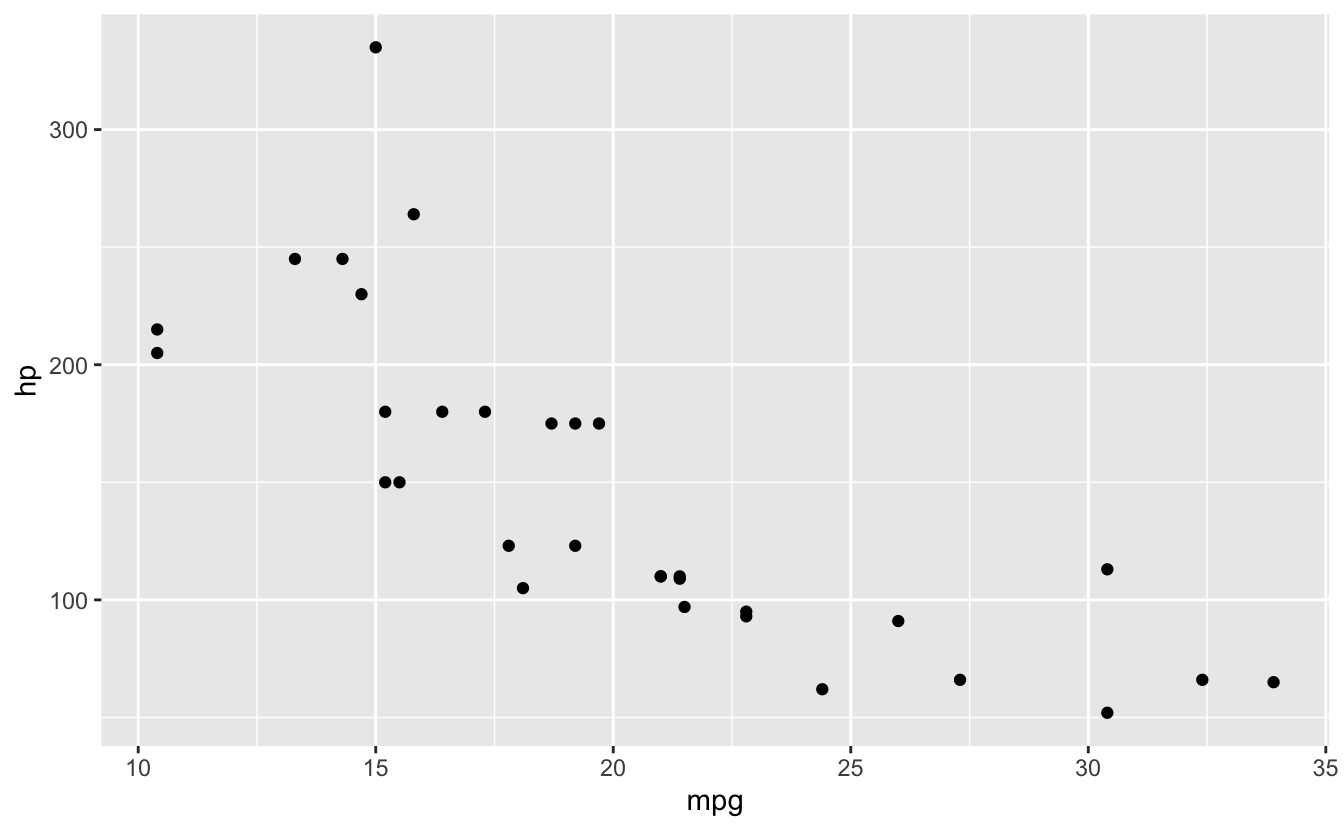
\includegraphics[width=1\linewidth]{mastering-r-through-errors_files/figure-latex/unnamed-chunk-1075-1} \end{center}

But ggplot2 has unique error patterns. Let's master them!

\section{ggplot2 Structure}\label{ggplot2-structure}

💡 \textbf{Key Insight: Grammar of Graphics}

\begin{Shaded}
\begin{Highlighting}[]
\CommentTok{\# Three essential components:}
\CommentTok{\# 1. Data}
\CommentTok{\# 2. Aesthetic mappings (aes)}
\CommentTok{\# 3. Geometric objects (geom)}

\CommentTok{\# Basic structure}
\FunctionTok{ggplot}\NormalTok{(}\AttributeTok{data =}\NormalTok{ mtcars, }\AttributeTok{mapping =} \FunctionTok{aes}\NormalTok{(}\AttributeTok{x =}\NormalTok{ mpg, }\AttributeTok{y =}\NormalTok{ hp)) }\SpecialCharTok{+}
  \FunctionTok{geom\_point}\NormalTok{()}

\CommentTok{\# Shortened (common)}
\FunctionTok{ggplot}\NormalTok{(mtcars, }\FunctionTok{aes}\NormalTok{(}\AttributeTok{x =}\NormalTok{ mpg, }\AttributeTok{y =}\NormalTok{ hp)) }\SpecialCharTok{+}
  \FunctionTok{geom\_point}\NormalTok{()}

\CommentTok{\# Can specify aes in geom instead}
\FunctionTok{ggplot}\NormalTok{(mtcars) }\SpecialCharTok{+}
  \FunctionTok{geom\_point}\NormalTok{(}\FunctionTok{aes}\NormalTok{(}\AttributeTok{x =}\NormalTok{ mpg, }\AttributeTok{y =}\NormalTok{ hp))}

\CommentTok{\# Or mix (useful for multiple layers)}
\FunctionTok{ggplot}\NormalTok{(mtcars, }\FunctionTok{aes}\NormalTok{(}\AttributeTok{x =}\NormalTok{ mpg, }\AttributeTok{y =}\NormalTok{ hp)) }\SpecialCharTok{+}
  \FunctionTok{geom\_point}\NormalTok{() }\SpecialCharTok{+}
  \FunctionTok{geom\_smooth}\NormalTok{()}
\CommentTok{\#\textgreater{} \textasciigrave{}geom\_smooth()\textasciigrave{} using method = \textquotesingle{}loess\textquotesingle{} and formula = \textquotesingle{}y \textasciitilde{} x\textquotesingle{}}
\end{Highlighting}
\end{Shaded}

\begin{center}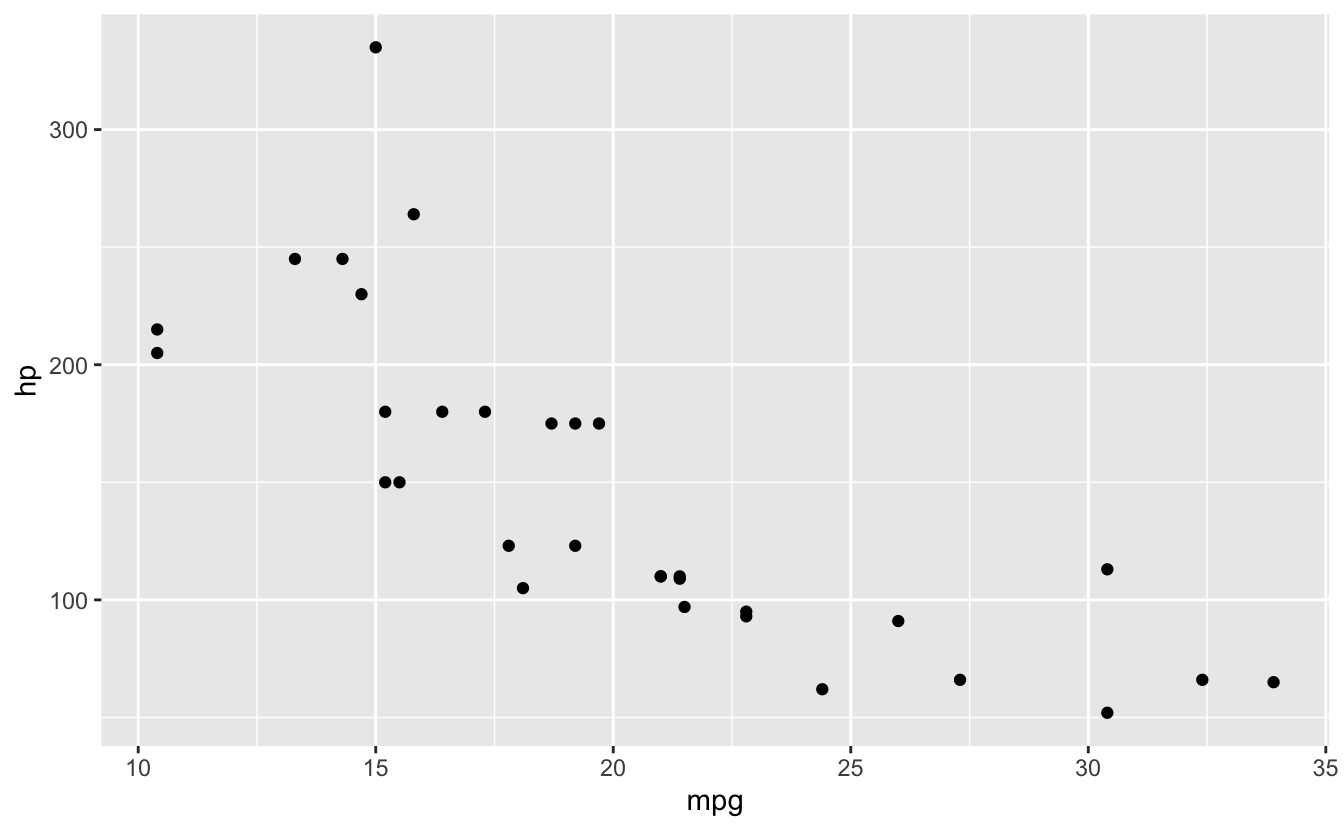
\includegraphics[width=1\linewidth]{mastering-r-through-errors_files/figure-latex/unnamed-chunk-1076-1} 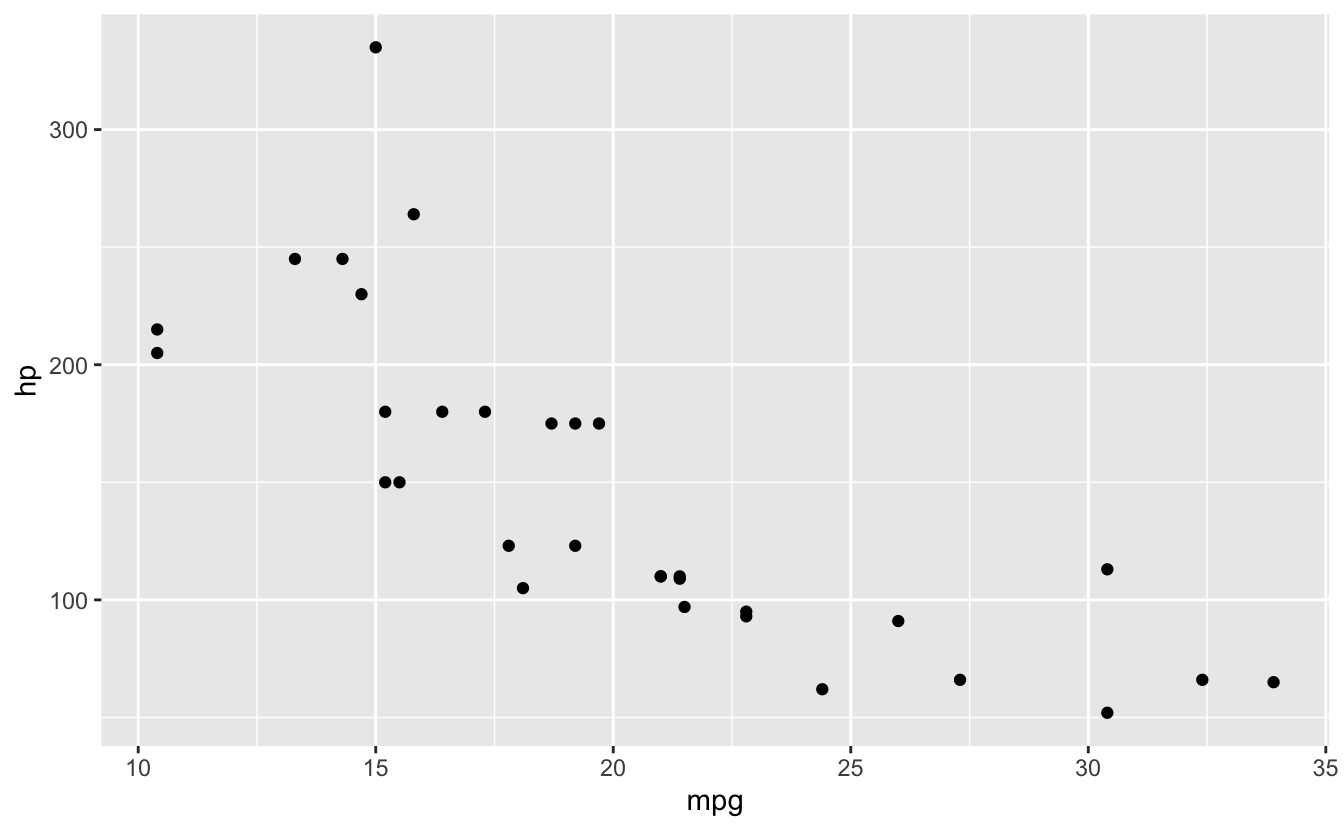
\includegraphics[width=1\linewidth]{mastering-r-through-errors_files/figure-latex/unnamed-chunk-1076-2} 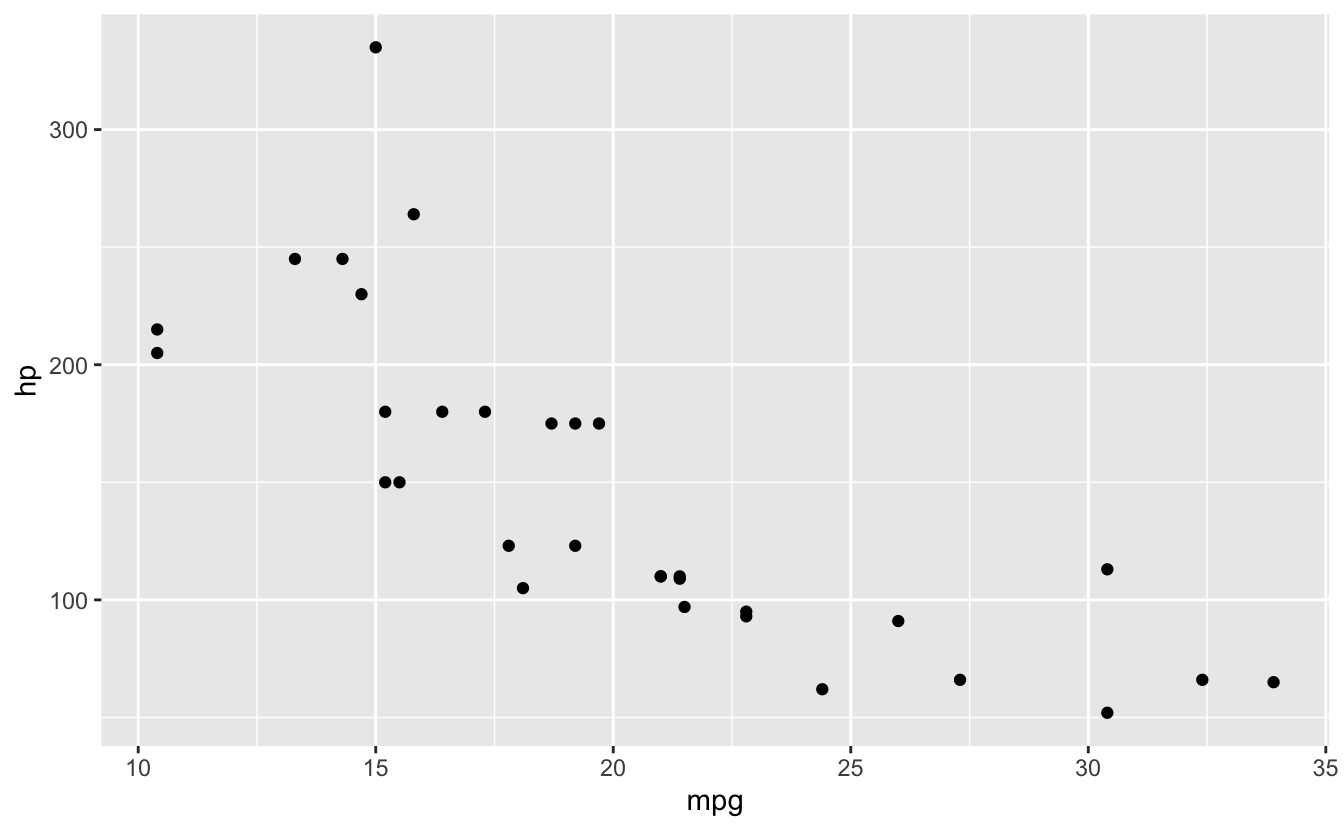
\includegraphics[width=1\linewidth]{mastering-r-through-errors_files/figure-latex/unnamed-chunk-1076-3} 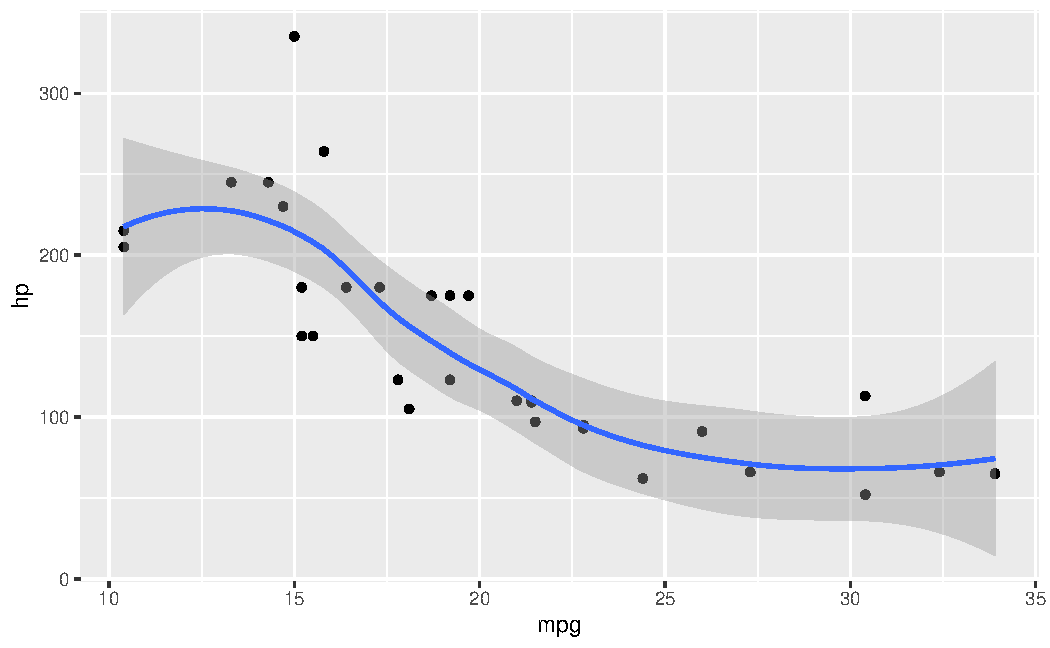
\includegraphics[width=1\linewidth]{mastering-r-through-errors_files/figure-latex/unnamed-chunk-1076-4} \end{center}

\textbf{Key principle:} Build plots in layers with \texttt{+}

\section{\texorpdfstring{Error \#1: \texttt{object\ not\ found} in aes()}{Error \#1: object not found in aes()}}\label{ggplot-object-not-found}

{⭐ BEGINNER} {🔍 SCOPE}

\subsection{The Error}\label{the-error-80}

\begin{Shaded}
\begin{Highlighting}[]
\FunctionTok{ggplot}\NormalTok{(mtcars, }\FunctionTok{aes}\NormalTok{(}\AttributeTok{x =}\NormalTok{ mpg, }\AttributeTok{y =}\NormalTok{ horsepower)) }\SpecialCharTok{+}
  \FunctionTok{geom\_point}\NormalTok{()}
\CommentTok{\#\textgreater{} Error in \textasciigrave{}geom\_point()\textasciigrave{}:}
\CommentTok{\#\textgreater{} ! Problem while computing aesthetics.}
\CommentTok{\#\textgreater{} i Error occurred in the 1st layer.}
\CommentTok{\#\textgreater{} Caused by error:}
\CommentTok{\#\textgreater{} ! object \textquotesingle{}horsepower\textquotesingle{} not found}
\end{Highlighting}
\end{Shaded}

🔴 \textbf{ERROR}

\begin{verbatim}
Error in FUN(X[[i]], ...) : object 'horsepower' not found
\end{verbatim}

\subsection{What It Means}\label{what-it-means-85}

The column name doesn't exist in the data.

\subsection{Common Causes}\label{common-causes-58}

\begin{Shaded}
\begin{Highlighting}[]
\CommentTok{\# Typo in column name}
\FunctionTok{ggplot}\NormalTok{(mtcars, }\FunctionTok{aes}\NormalTok{(}\AttributeTok{x =}\NormalTok{ mpgg, }\AttributeTok{y =}\NormalTok{ hp)) }\SpecialCharTok{+}
  \FunctionTok{geom\_point}\NormalTok{()}
\CommentTok{\#\textgreater{} Error in \textasciigrave{}geom\_point()\textasciigrave{}:}
\CommentTok{\#\textgreater{} ! Problem while computing aesthetics.}
\CommentTok{\#\textgreater{} i Error occurred in the 1st layer.}
\CommentTok{\#\textgreater{} Caused by error:}
\CommentTok{\#\textgreater{} ! object \textquotesingle{}mpgg\textquotesingle{} not found}

\CommentTok{\# Wrong dataset}
\FunctionTok{ggplot}\NormalTok{(iris, }\FunctionTok{aes}\NormalTok{(}\AttributeTok{x =}\NormalTok{ mpg, }\AttributeTok{y =}\NormalTok{ hp)) }\SpecialCharTok{+}
  \FunctionTok{geom\_point}\NormalTok{()}
\CommentTok{\#\textgreater{} Error in \textasciigrave{}geom\_point()\textasciigrave{}:}
\CommentTok{\#\textgreater{} ! Problem while computing aesthetics.}
\CommentTok{\#\textgreater{} i Error occurred in the 1st layer.}
\CommentTok{\#\textgreater{} Caused by error:}
\CommentTok{\#\textgreater{} ! object \textquotesingle{}hp\textquotesingle{} not found}

\CommentTok{\# Forgot to create column}
\FunctionTok{ggplot}\NormalTok{(mtcars, }\FunctionTok{aes}\NormalTok{(}\AttributeTok{x =}\NormalTok{ mpg, }\AttributeTok{y =}\NormalTok{ efficiency)) }\SpecialCharTok{+}
  \FunctionTok{geom\_point}\NormalTok{()}
\CommentTok{\#\textgreater{} Error in \textasciigrave{}geom\_point()\textasciigrave{}:}
\CommentTok{\#\textgreater{} ! Problem while computing aesthetics.}
\CommentTok{\#\textgreater{} i Error occurred in the 1st layer.}
\CommentTok{\#\textgreater{} Caused by error:}
\CommentTok{\#\textgreater{} ! object \textquotesingle{}efficiency\textquotesingle{} not found}
\end{Highlighting}
\end{Shaded}

\subsection{Solutions}\label{solutions-96}

✅ \textbf{SOLUTION 1: Check Column Names}

\begin{Shaded}
\begin{Highlighting}[]
\CommentTok{\# Verify columns}
\FunctionTok{names}\NormalTok{(mtcars)}
\CommentTok{\#\textgreater{}  [1] "mpg"        "cyl"        "disp"       "hp"         "drat"      }
\CommentTok{\#\textgreater{}  [6] "wt"         "qsec"       "vs"         "am"         "gear"      }
\CommentTok{\#\textgreater{} [11] "carb"       "cyl\_factor"}

\CommentTok{\# Use correct name}
\FunctionTok{ggplot}\NormalTok{(mtcars, }\FunctionTok{aes}\NormalTok{(}\AttributeTok{x =}\NormalTok{ mpg, }\AttributeTok{y =}\NormalTok{ hp)) }\SpecialCharTok{+}
  \FunctionTok{geom\_point}\NormalTok{()}
\end{Highlighting}
\end{Shaded}

\begin{center}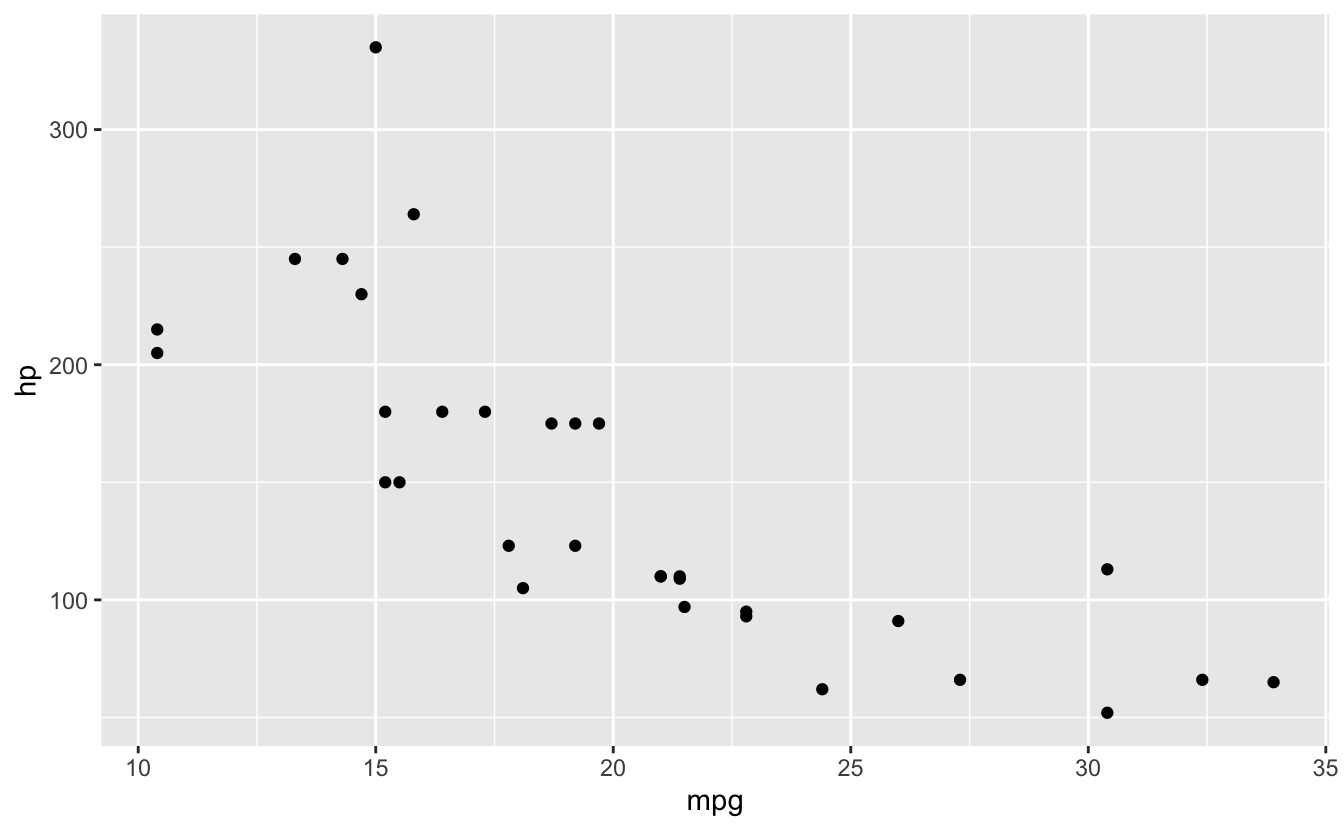
\includegraphics[width=1\linewidth]{mastering-r-through-errors_files/figure-latex/unnamed-chunk-1079-1} \end{center}

✅ \textbf{SOLUTION 2: Create Column First}

\begin{Shaded}
\begin{Highlighting}[]
\FunctionTok{library}\NormalTok{(dplyr)}

\NormalTok{mtcars }\SpecialCharTok{\%\textgreater{}\%}
  \FunctionTok{mutate}\NormalTok{(}\AttributeTok{efficiency =}\NormalTok{ mpg }\SpecialCharTok{/}\NormalTok{ hp) }\SpecialCharTok{\%\textgreater{}\%}
  \FunctionTok{ggplot}\NormalTok{(}\FunctionTok{aes}\NormalTok{(}\AttributeTok{x =}\NormalTok{ hp, }\AttributeTok{y =}\NormalTok{ efficiency)) }\SpecialCharTok{+}
  \FunctionTok{geom\_point}\NormalTok{()}
\end{Highlighting}
\end{Shaded}

\begin{center}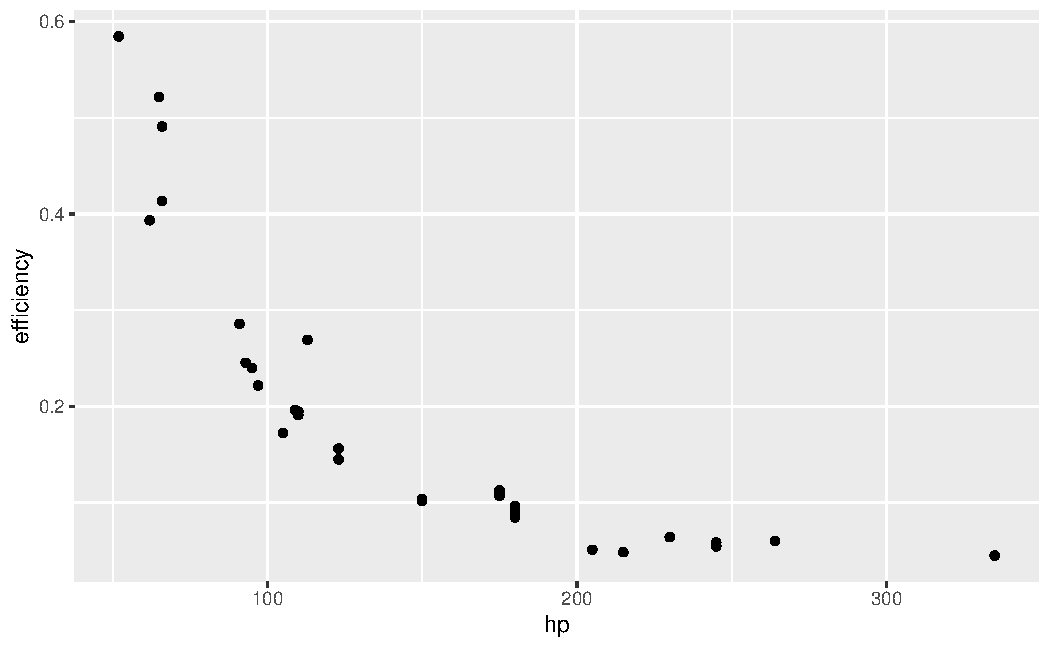
\includegraphics[width=1\linewidth]{mastering-r-through-errors_files/figure-latex/unnamed-chunk-1080-1} \end{center}

\section{\texorpdfstring{Error \#2: Using \texttt{+} vs \texttt{\%\textgreater{}\%}}{Error \#2: Using + vs \%\textgreater\%}}\label{ggplot-plus-vs-pipe}

{⭐ BEGINNER} {🔤 SYNTAX}

\subsection{The Error}\label{the-error-81}

\begin{Shaded}
\begin{Highlighting}[]
\FunctionTok{library}\NormalTok{(dplyr)}

\NormalTok{mtcars }\SpecialCharTok{\%\textgreater{}\%}
  \FunctionTok{filter}\NormalTok{(cyl }\SpecialCharTok{==} \DecValTok{4}\NormalTok{) }\SpecialCharTok{\%\textgreater{}\%}
  \FunctionTok{ggplot}\NormalTok{(}\FunctionTok{aes}\NormalTok{(}\AttributeTok{x =}\NormalTok{ mpg, }\AttributeTok{y =}\NormalTok{ hp)) }\SpecialCharTok{\%\textgreater{}\%}  \CommentTok{\# Wrong operator!}
  \FunctionTok{geom\_point}\NormalTok{()}
\CommentTok{\#\textgreater{} Error in \textasciigrave{}geom\_point()\textasciigrave{}:}
\CommentTok{\#\textgreater{} ! \textasciigrave{}mapping\textasciigrave{} must be created by \textasciigrave{}aes()\textasciigrave{}.}
\CommentTok{\#\textgreater{} x You\textquotesingle{}ve supplied a \textless{}ggplot2::ggplot\textgreater{} object.}
\CommentTok{\#\textgreater{} i Did you use \textasciigrave{}\%\textgreater{}\%\textasciigrave{} or \textasciigrave{}|\textgreater{}\textasciigrave{} instead of \textasciigrave{}+\textasciigrave{}?}
\end{Highlighting}
\end{Shaded}

🔴 \textbf{ERROR}

\begin{verbatim}
Error in geom_point(.) : 
  Cannot use `+` with a ggplot object. Did you accidentally use `%>%` instead of `+`?
\end{verbatim}

\subsection{What It Means}\label{what-it-means-86}

Must use \texttt{+} to add ggplot2 layers, not \texttt{\%\textgreater{}\%}.

\subsection{Solutions}\label{solutions-97}

✅ \textbf{SOLUTION: Use + for ggplot layers}

\begin{Shaded}
\begin{Highlighting}[]
\CommentTok{\# Correct: + for ggplot}
\NormalTok{mtcars }\SpecialCharTok{\%\textgreater{}\%}
  \FunctionTok{filter}\NormalTok{(cyl }\SpecialCharTok{==} \DecValTok{4}\NormalTok{) }\SpecialCharTok{\%\textgreater{}\%}
  \FunctionTok{ggplot}\NormalTok{(}\FunctionTok{aes}\NormalTok{(}\AttributeTok{x =}\NormalTok{ mpg, }\AttributeTok{y =}\NormalTok{ hp)) }\SpecialCharTok{+}  \CommentTok{\# Use +}
  \FunctionTok{geom\_point}\NormalTok{()}

\CommentTok{\# Pipe data into ggplot, then use +}
\NormalTok{mtcars }\SpecialCharTok{\%\textgreater{}\%}
  \FunctionTok{filter}\NormalTok{(cyl }\SpecialCharTok{==} \DecValTok{4}\NormalTok{) }\SpecialCharTok{\%\textgreater{}\%}
  \FunctionTok{ggplot}\NormalTok{(}\FunctionTok{aes}\NormalTok{(}\AttributeTok{x =}\NormalTok{ mpg, }\AttributeTok{y =}\NormalTok{ hp)) }\SpecialCharTok{+}
  \FunctionTok{geom\_point}\NormalTok{() }\SpecialCharTok{+}
  \FunctionTok{theme\_minimal}\NormalTok{()}
\end{Highlighting}
\end{Shaded}

\begin{center}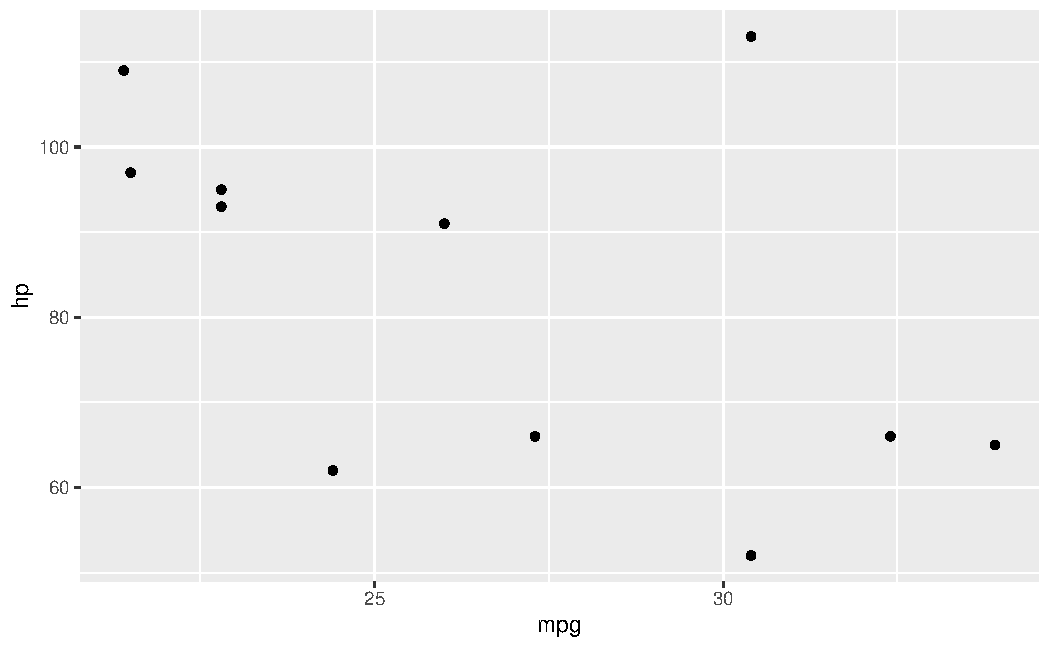
\includegraphics[width=1\linewidth]{mastering-r-through-errors_files/figure-latex/unnamed-chunk-1082-1} 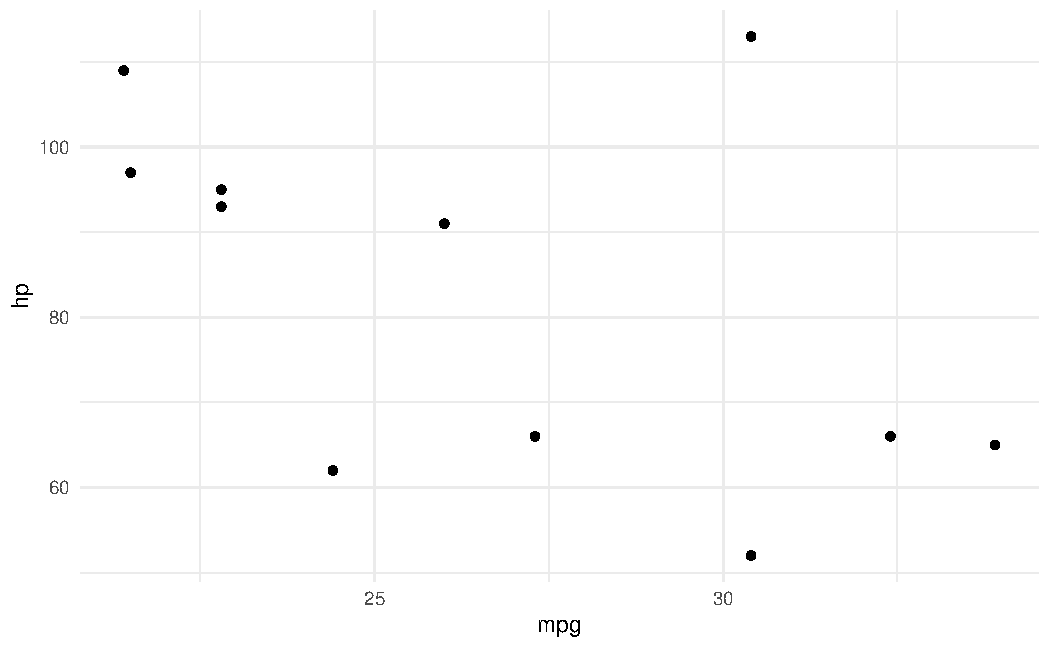
\includegraphics[width=1\linewidth]{mastering-r-through-errors_files/figure-latex/unnamed-chunk-1082-2} \end{center}

\section{Aesthetics (aes)}\label{aesthetics-aes}

💡 \textbf{Key Insight: Aesthetic Mappings}

\begin{Shaded}
\begin{Highlighting}[]
\CommentTok{\# Map variables to visual properties}
\FunctionTok{ggplot}\NormalTok{(mtcars, }\FunctionTok{aes}\NormalTok{(}\AttributeTok{x =}\NormalTok{ mpg, }\AttributeTok{y =}\NormalTok{ hp, }\AttributeTok{color =} \FunctionTok{factor}\NormalTok{(cyl))) }\SpecialCharTok{+}
  \FunctionTok{geom\_point}\NormalTok{()}

\CommentTok{\# Common aesthetics:}
\CommentTok{\# x, y {-} position}
\CommentTok{\# color {-} point/line color}
\CommentTok{\# fill {-} area fill color}
\CommentTok{\# size {-} point/line size}
\CommentTok{\# shape {-} point shape}
\CommentTok{\# alpha {-} transparency}
\CommentTok{\# linetype {-} line pattern}

\CommentTok{\# Multiple aesthetics}
\FunctionTok{ggplot}\NormalTok{(mtcars, }\FunctionTok{aes}\NormalTok{(}\AttributeTok{x =}\NormalTok{ mpg, }\AttributeTok{y =}\NormalTok{ hp, }
                   \AttributeTok{color =} \FunctionTok{factor}\NormalTok{(cyl),}
                   \AttributeTok{size =}\NormalTok{ wt)) }\SpecialCharTok{+}
  \FunctionTok{geom\_point}\NormalTok{()}

\CommentTok{\# Set vs map}
\FunctionTok{ggplot}\NormalTok{(mtcars, }\FunctionTok{aes}\NormalTok{(}\AttributeTok{x =}\NormalTok{ mpg, }\AttributeTok{y =}\NormalTok{ hp)) }\SpecialCharTok{+}
  \FunctionTok{geom\_point}\NormalTok{(}\AttributeTok{color =} \StringTok{"blue"}\NormalTok{)  }\CommentTok{\# Set: all points blue}

\FunctionTok{ggplot}\NormalTok{(mtcars, }\FunctionTok{aes}\NormalTok{(}\AttributeTok{x =}\NormalTok{ mpg, }\AttributeTok{y =}\NormalTok{ hp, }\AttributeTok{color =} \FunctionTok{factor}\NormalTok{(cyl))) }\SpecialCharTok{+}
  \FunctionTok{geom\_point}\NormalTok{()  }\CommentTok{\# Map: color varies by cyl}
\end{Highlighting}
\end{Shaded}

\begin{center}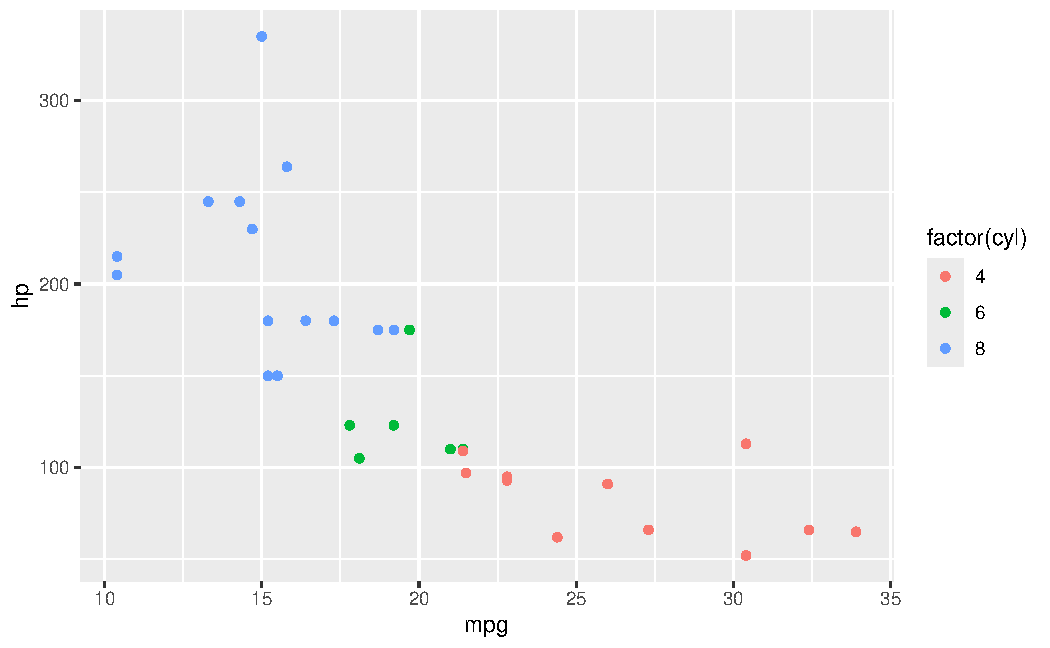
\includegraphics[width=1\linewidth]{mastering-r-through-errors_files/figure-latex/unnamed-chunk-1083-1} 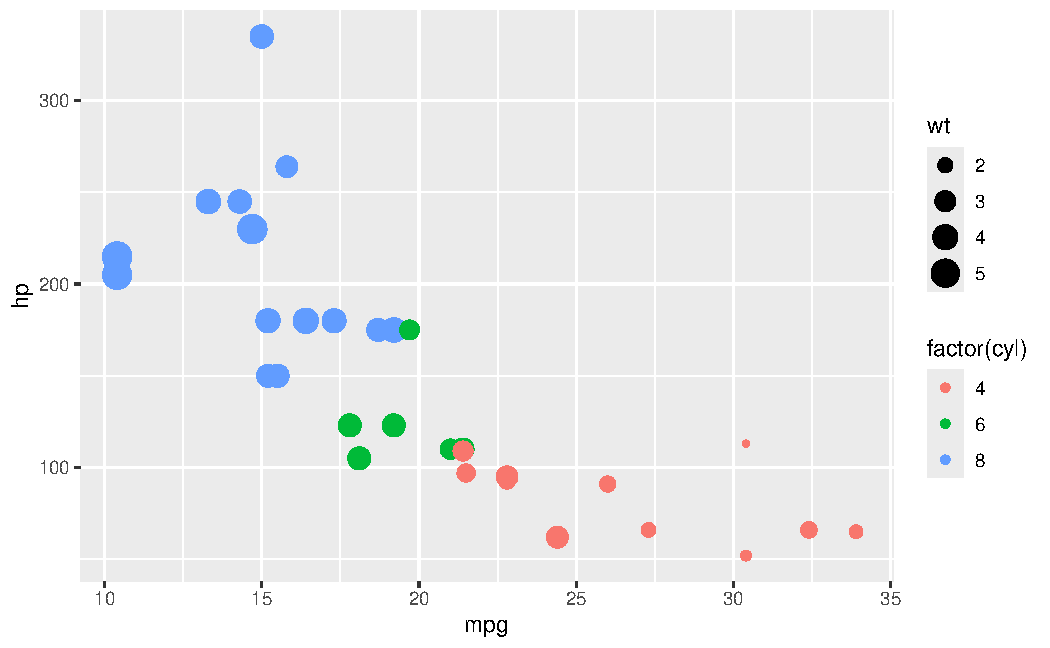
\includegraphics[width=1\linewidth]{mastering-r-through-errors_files/figure-latex/unnamed-chunk-1083-2} 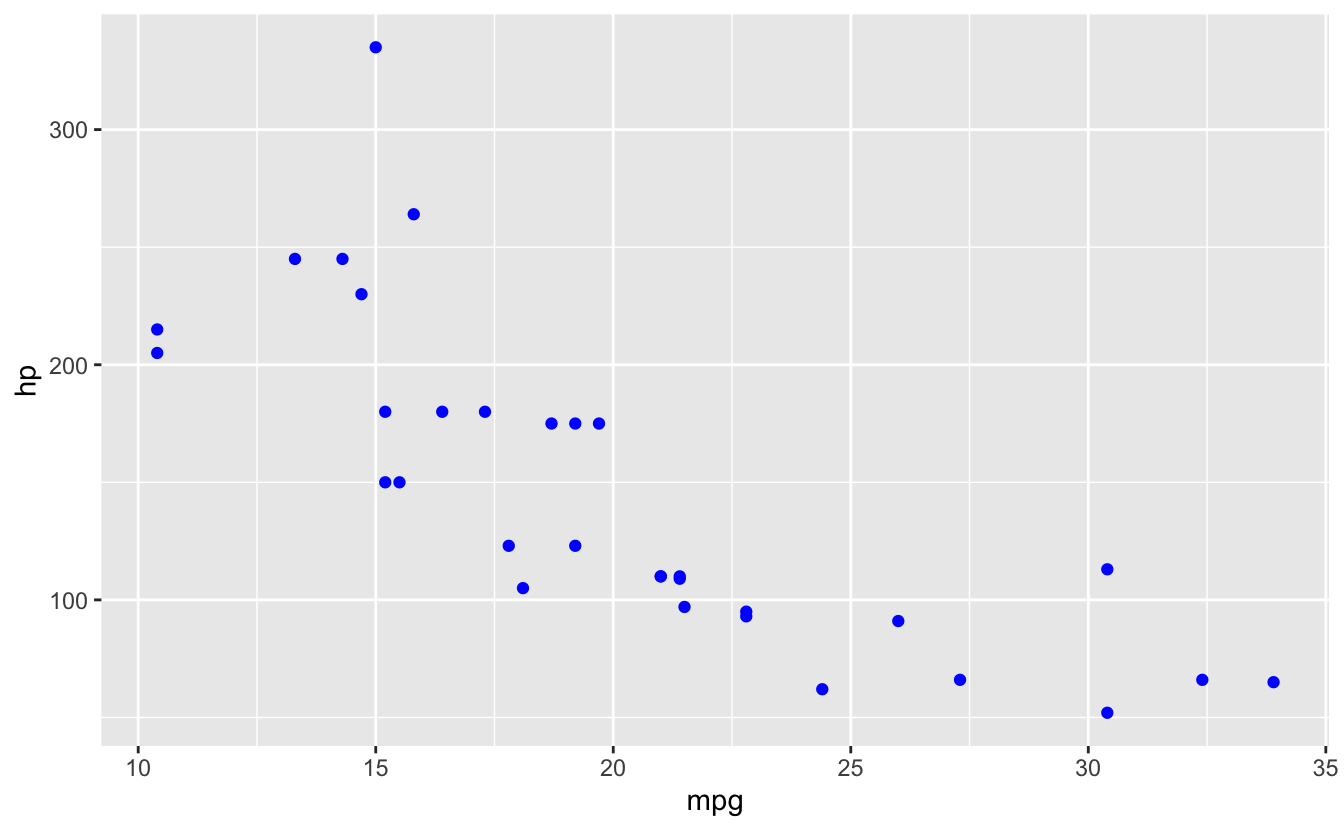
\includegraphics[width=1\linewidth]{mastering-r-through-errors_files/figure-latex/unnamed-chunk-1083-3} 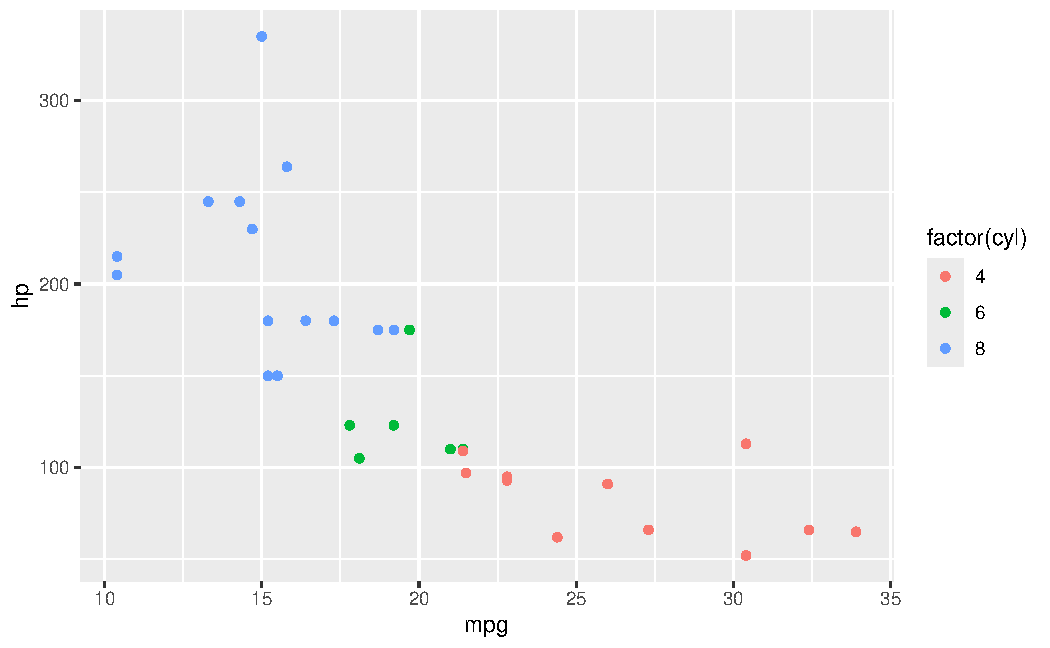
\includegraphics[width=1\linewidth]{mastering-r-through-errors_files/figure-latex/unnamed-chunk-1083-4} \end{center}

\section{Error \#3: Aesthetic outside aes()}\label{aesthetic-outside-aes}

{⭐⭐ INTERMEDIATE} {🧠 LOGIC}

\subsection{The Error}\label{the-error-82}

\begin{Shaded}
\begin{Highlighting}[]
\CommentTok{\# Trying to map cyl to color outside aes()}
\FunctionTok{ggplot}\NormalTok{(mtcars) }\SpecialCharTok{+}
  \FunctionTok{geom\_point}\NormalTok{(}\FunctionTok{aes}\NormalTok{(}\AttributeTok{x =}\NormalTok{ mpg, }\AttributeTok{y =}\NormalTok{ hp), }\AttributeTok{color =}\NormalTok{ cyl)}
\CommentTok{\#\textgreater{} Error: object \textquotesingle{}cyl\textquotesingle{} not found}
\end{Highlighting}
\end{Shaded}

🔴 \textbf{ERROR}

\begin{verbatim}
Error in layer(...) : object 'cyl' not found
\end{verbatim}

\subsection{What It Means}\label{what-it-means-87}

Variable mappings must be inside \texttt{aes()}.

\subsection{Common Causes}\label{common-causes-59}

\begin{Shaded}
\begin{Highlighting}[]
\CommentTok{\# Want color by variable}
\FunctionTok{ggplot}\NormalTok{(mtcars) }\SpecialCharTok{+}
  \FunctionTok{geom\_point}\NormalTok{(}\FunctionTok{aes}\NormalTok{(}\AttributeTok{x =}\NormalTok{ mpg, }\AttributeTok{y =}\NormalTok{ hp), }\AttributeTok{color =} \FunctionTok{factor}\NormalTok{(cyl))}
\CommentTok{\#\textgreater{} Error: object \textquotesingle{}cyl\textquotesingle{} not found}

\CommentTok{\# Want size by variable}
\FunctionTok{ggplot}\NormalTok{(mtcars) }\SpecialCharTok{+}
  \FunctionTok{geom\_point}\NormalTok{(}\FunctionTok{aes}\NormalTok{(}\AttributeTok{x =}\NormalTok{ mpg, }\AttributeTok{y =}\NormalTok{ hp), }\AttributeTok{size =}\NormalTok{ wt)}
\CommentTok{\#\textgreater{} Error: object \textquotesingle{}wt\textquotesingle{} not found}
\end{Highlighting}
\end{Shaded}

\subsection{Solutions}\label{solutions-98}

✅ \textbf{SOLUTION: Put Variable Mappings in aes()}

\begin{Shaded}
\begin{Highlighting}[]
\CommentTok{\# Correct: color mapping inside aes}
\FunctionTok{ggplot}\NormalTok{(mtcars) }\SpecialCharTok{+}
  \FunctionTok{geom\_point}\NormalTok{(}\FunctionTok{aes}\NormalTok{(}\AttributeTok{x =}\NormalTok{ mpg, }\AttributeTok{y =}\NormalTok{ hp, }\AttributeTok{color =} \FunctionTok{factor}\NormalTok{(cyl)))}

\CommentTok{\# Can be in ggplot() aes}
\FunctionTok{ggplot}\NormalTok{(mtcars, }\FunctionTok{aes}\NormalTok{(}\AttributeTok{x =}\NormalTok{ mpg, }\AttributeTok{y =}\NormalTok{ hp, }\AttributeTok{color =} \FunctionTok{factor}\NormalTok{(cyl))) }\SpecialCharTok{+}
  \FunctionTok{geom\_point}\NormalTok{()}

\CommentTok{\# Fixed values go OUTSIDE aes}
\FunctionTok{ggplot}\NormalTok{(mtcars, }\FunctionTok{aes}\NormalTok{(}\AttributeTok{x =}\NormalTok{ mpg, }\AttributeTok{y =}\NormalTok{ hp)) }\SpecialCharTok{+}
  \FunctionTok{geom\_point}\NormalTok{(}\AttributeTok{color =} \StringTok{"blue"}\NormalTok{, }\AttributeTok{size =} \DecValTok{3}\NormalTok{)  }\CommentTok{\# All points same}
\end{Highlighting}
\end{Shaded}

\begin{center}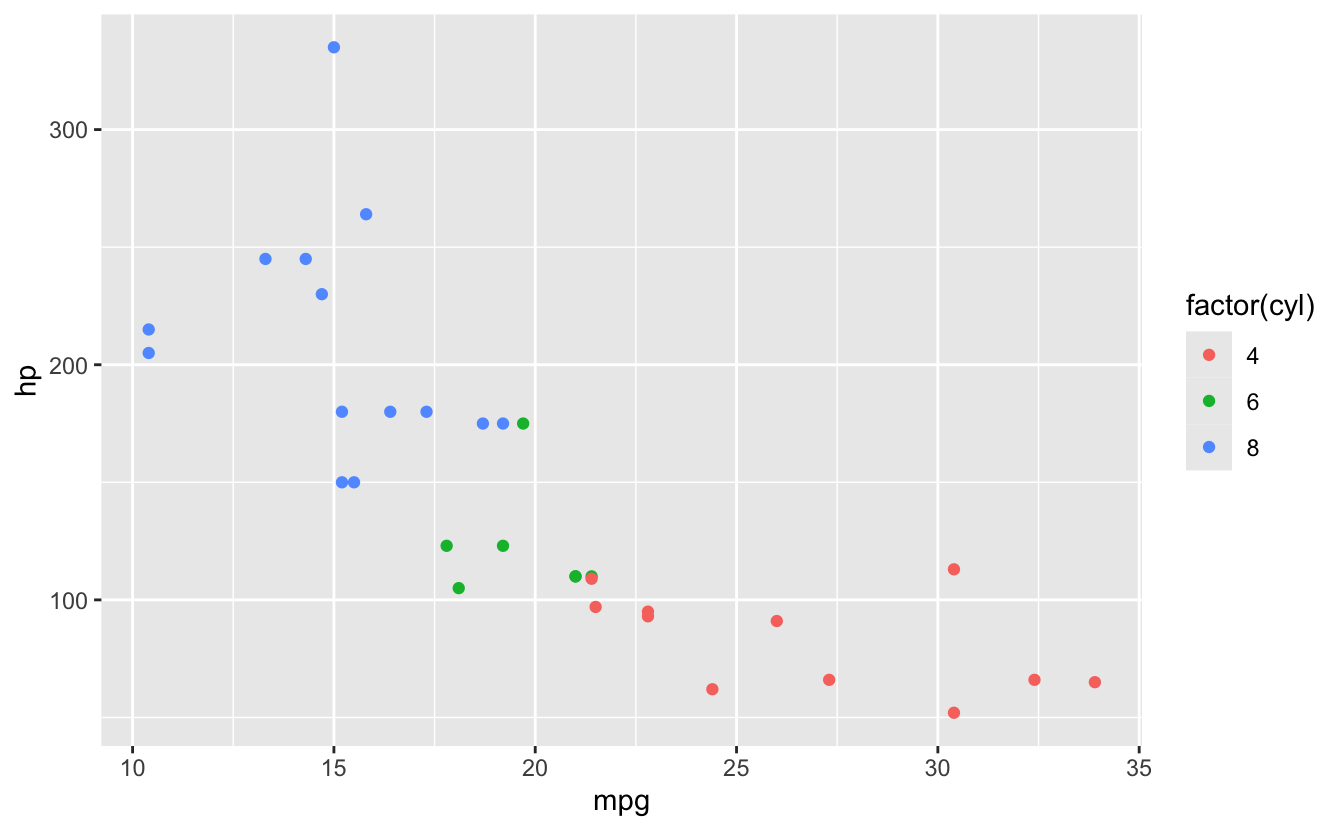
\includegraphics[width=1\linewidth]{mastering-r-through-errors_files/figure-latex/unnamed-chunk-1086-1} 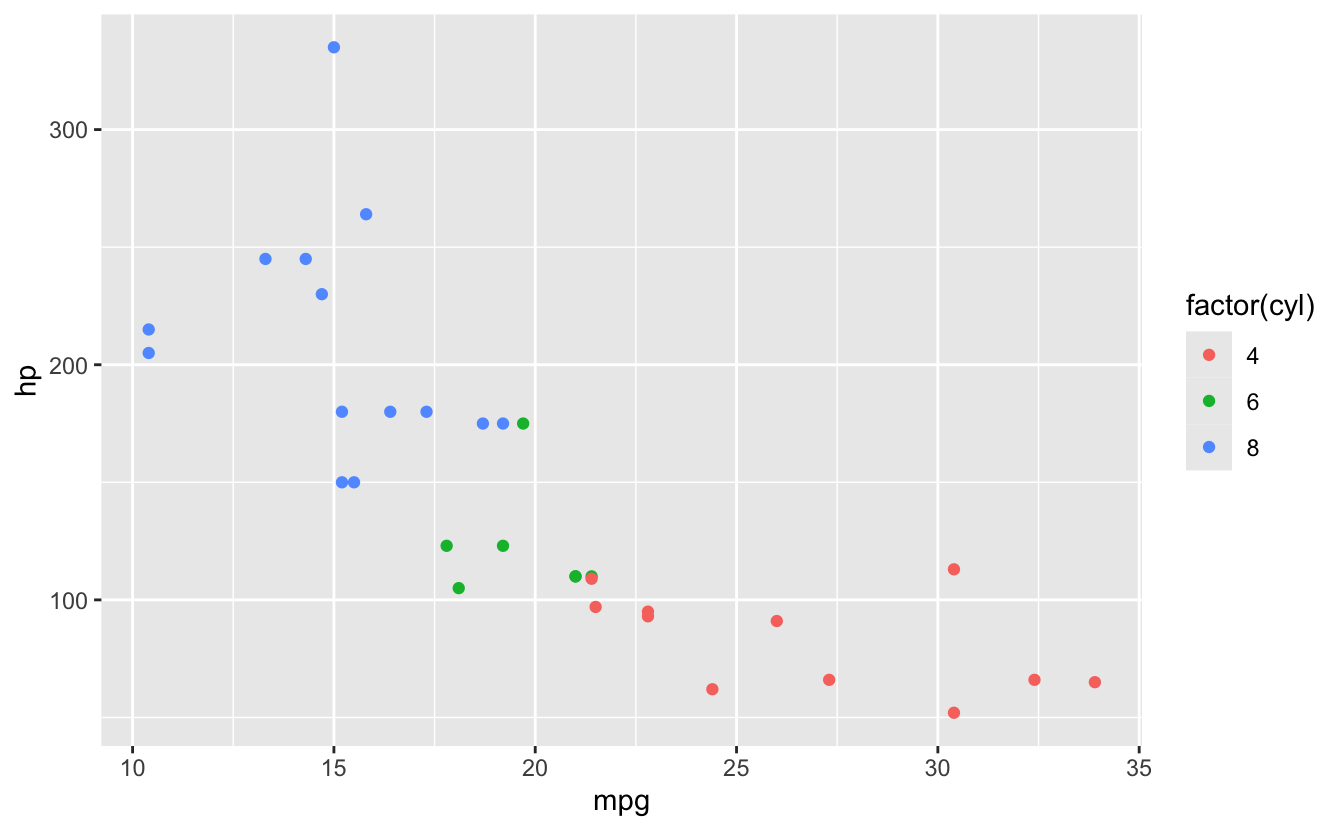
\includegraphics[width=1\linewidth]{mastering-r-through-errors_files/figure-latex/unnamed-chunk-1086-2} 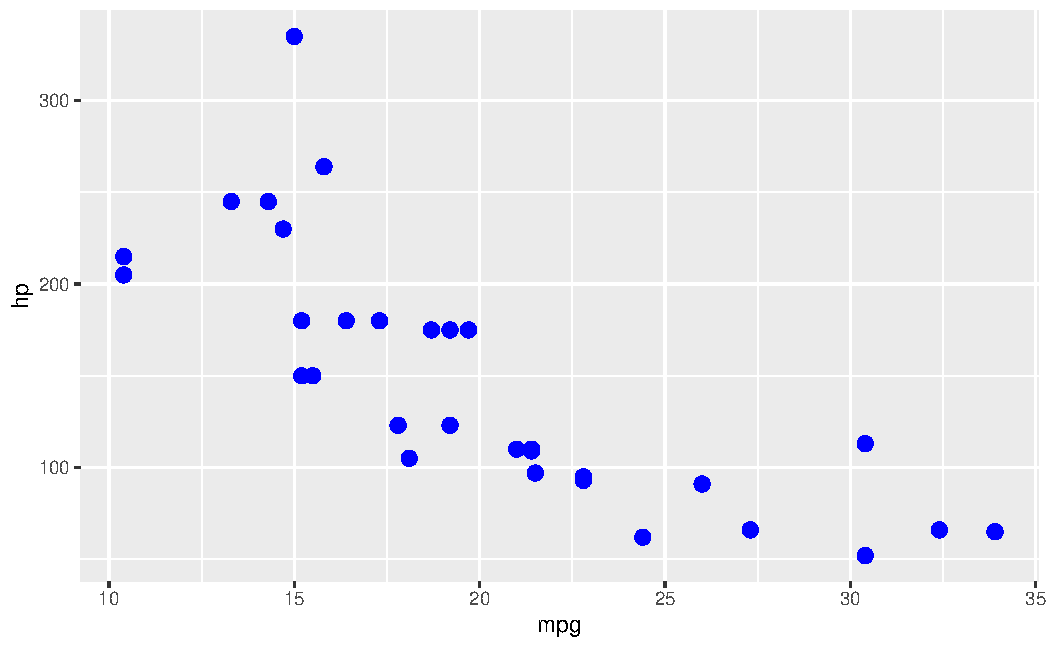
\includegraphics[width=1\linewidth]{mastering-r-through-errors_files/figure-latex/unnamed-chunk-1086-3} \end{center}

⚠️ \textbf{Common Confusion: Inside vs Outside aes()}

\begin{Shaded}
\begin{Highlighting}[]
\CommentTok{\# INSIDE aes(): varies by data}
\FunctionTok{ggplot}\NormalTok{(mtcars, }\FunctionTok{aes}\NormalTok{(}\AttributeTok{x =}\NormalTok{ mpg, }\AttributeTok{y =}\NormalTok{ hp, }\AttributeTok{color =} \FunctionTok{factor}\NormalTok{(cyl))) }\SpecialCharTok{+}
  \FunctionTok{geom\_point}\NormalTok{()  }\CommentTok{\# Color varies by cyl}

\CommentTok{\# OUTSIDE aes(): fixed for all}
\FunctionTok{ggplot}\NormalTok{(mtcars, }\FunctionTok{aes}\NormalTok{(}\AttributeTok{x =}\NormalTok{ mpg, }\AttributeTok{y =}\NormalTok{ hp)) }\SpecialCharTok{+}
  \FunctionTok{geom\_point}\NormalTok{(}\AttributeTok{color =} \StringTok{"red"}\NormalTok{)  }\CommentTok{\# All points red}

\CommentTok{\# Wrong: puts string in aes}
\FunctionTok{ggplot}\NormalTok{(mtcars, }\FunctionTok{aes}\NormalTok{(}\AttributeTok{x =}\NormalTok{ mpg, }\AttributeTok{y =}\NormalTok{ hp, }\AttributeTok{color =} \StringTok{"red"}\NormalTok{)) }\SpecialCharTok{+}
  \FunctionTok{geom\_point}\NormalTok{()  }\CommentTok{\# Creates legend for "red"!}
\end{Highlighting}
\end{Shaded}

\begin{center}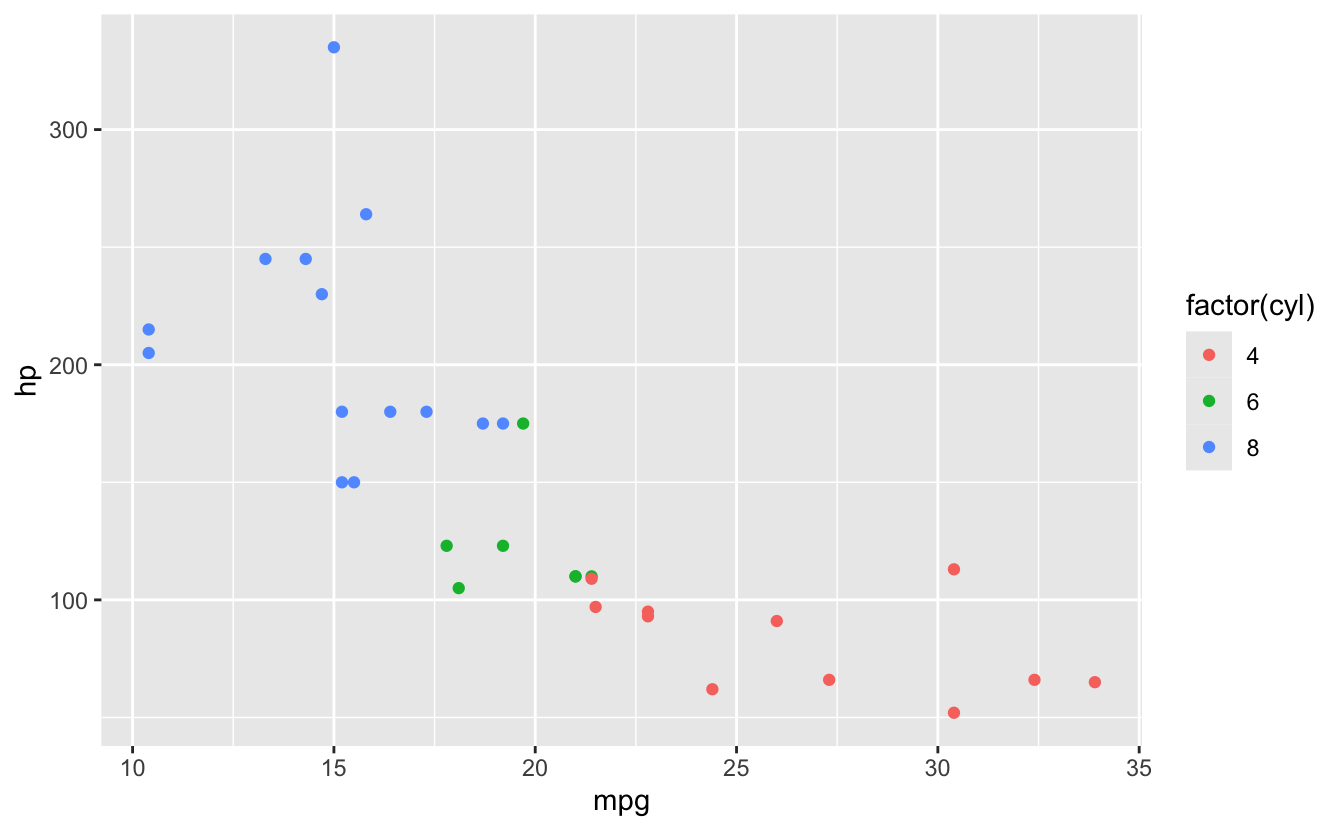
\includegraphics[width=1\linewidth]{mastering-r-through-errors_files/figure-latex/unnamed-chunk-1087-1} 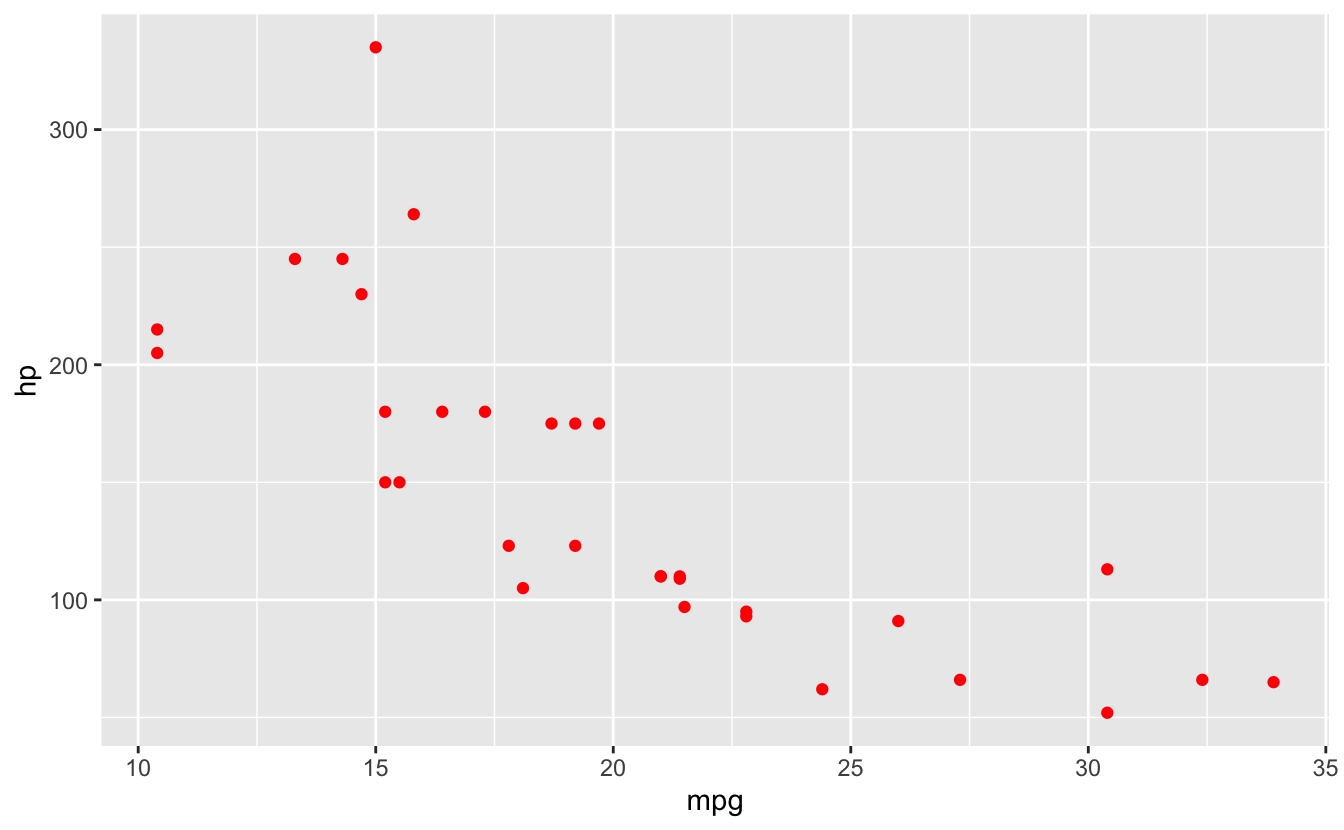
\includegraphics[width=1\linewidth]{mastering-r-through-errors_files/figure-latex/unnamed-chunk-1087-2} 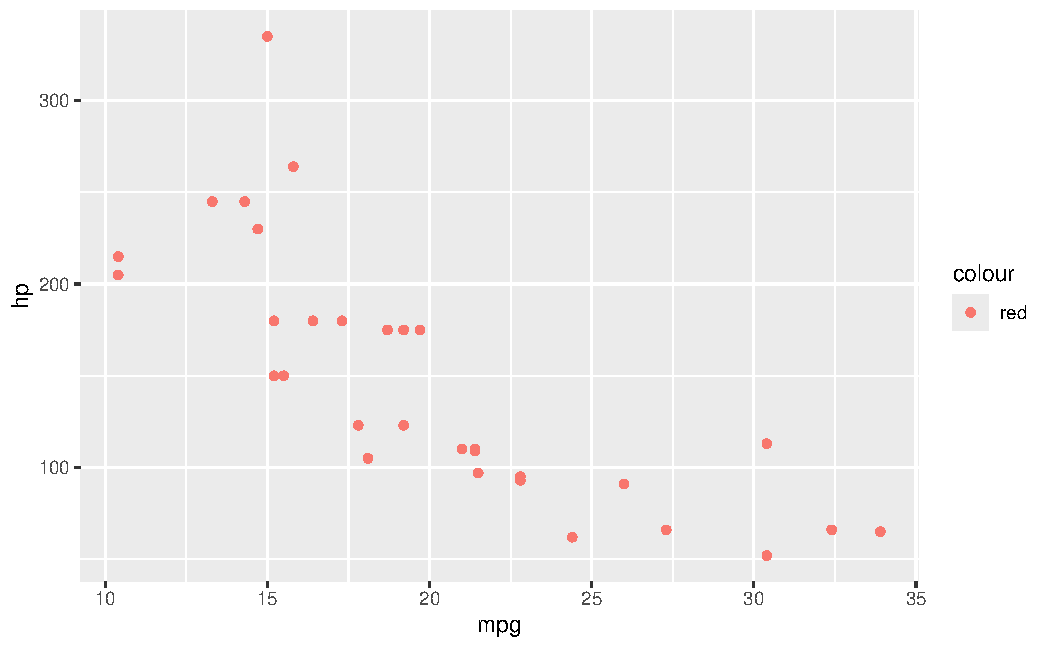
\includegraphics[width=1\linewidth]{mastering-r-through-errors_files/figure-latex/unnamed-chunk-1087-3} \end{center}

\section{Common geoms}\label{common-geoms}

💡 \textbf{Key Insight: Geometric Objects}

\begin{Shaded}
\begin{Highlighting}[]
\CommentTok{\# Points}
\FunctionTok{ggplot}\NormalTok{(mtcars, }\FunctionTok{aes}\NormalTok{(}\AttributeTok{x =}\NormalTok{ mpg, }\AttributeTok{y =}\NormalTok{ hp)) }\SpecialCharTok{+}
  \FunctionTok{geom\_point}\NormalTok{()}

\CommentTok{\# Lines}
\FunctionTok{ggplot}\NormalTok{(economics, }\FunctionTok{aes}\NormalTok{(}\AttributeTok{x =}\NormalTok{ date, }\AttributeTok{y =}\NormalTok{ unemploy)) }\SpecialCharTok{+}
  \FunctionTok{geom\_line}\NormalTok{()}

\CommentTok{\# Bars}
\FunctionTok{ggplot}\NormalTok{(mtcars, }\FunctionTok{aes}\NormalTok{(}\AttributeTok{x =} \FunctionTok{factor}\NormalTok{(cyl))) }\SpecialCharTok{+}
  \FunctionTok{geom\_bar}\NormalTok{()}

\CommentTok{\# Histogram}
\FunctionTok{ggplot}\NormalTok{(mtcars, }\FunctionTok{aes}\NormalTok{(}\AttributeTok{x =}\NormalTok{ mpg)) }\SpecialCharTok{+}
  \FunctionTok{geom\_histogram}\NormalTok{(}\AttributeTok{bins =} \DecValTok{10}\NormalTok{)}

\CommentTok{\# Boxplot}
\FunctionTok{ggplot}\NormalTok{(mtcars, }\FunctionTok{aes}\NormalTok{(}\AttributeTok{x =} \FunctionTok{factor}\NormalTok{(cyl), }\AttributeTok{y =}\NormalTok{ mpg)) }\SpecialCharTok{+}
  \FunctionTok{geom\_boxplot}\NormalTok{()}

\CommentTok{\# Smooth}
\FunctionTok{ggplot}\NormalTok{(mtcars, }\FunctionTok{aes}\NormalTok{(}\AttributeTok{x =}\NormalTok{ mpg, }\AttributeTok{y =}\NormalTok{ hp)) }\SpecialCharTok{+}
  \FunctionTok{geom\_point}\NormalTok{() }\SpecialCharTok{+}
  \FunctionTok{geom\_smooth}\NormalTok{(}\AttributeTok{method =} \StringTok{"lm"}\NormalTok{)}
\CommentTok{\#\textgreater{} \textasciigrave{}geom\_smooth()\textasciigrave{} using formula = \textquotesingle{}y \textasciitilde{} x\textquotesingle{}}

\CommentTok{\# Text}
\FunctionTok{ggplot}\NormalTok{(mtcars, }\FunctionTok{aes}\NormalTok{(}\AttributeTok{x =}\NormalTok{ mpg, }\AttributeTok{y =}\NormalTok{ hp, }\AttributeTok{label =} \FunctionTok{rownames}\NormalTok{(mtcars))) }\SpecialCharTok{+}
  \FunctionTok{geom\_text}\NormalTok{(}\AttributeTok{size =} \DecValTok{3}\NormalTok{)}
\end{Highlighting}
\end{Shaded}

\begin{center}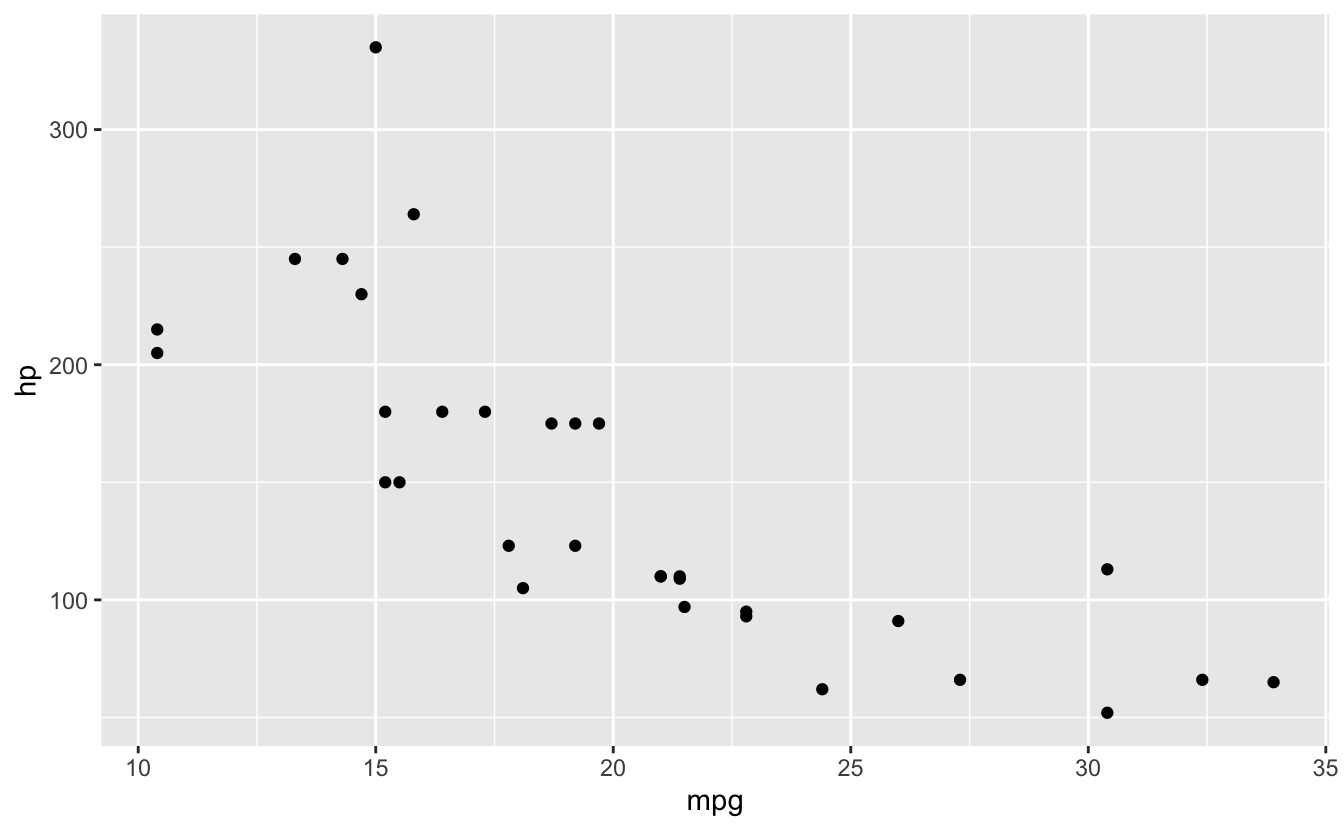
\includegraphics[width=1\linewidth]{mastering-r-through-errors_files/figure-latex/unnamed-chunk-1088-1} 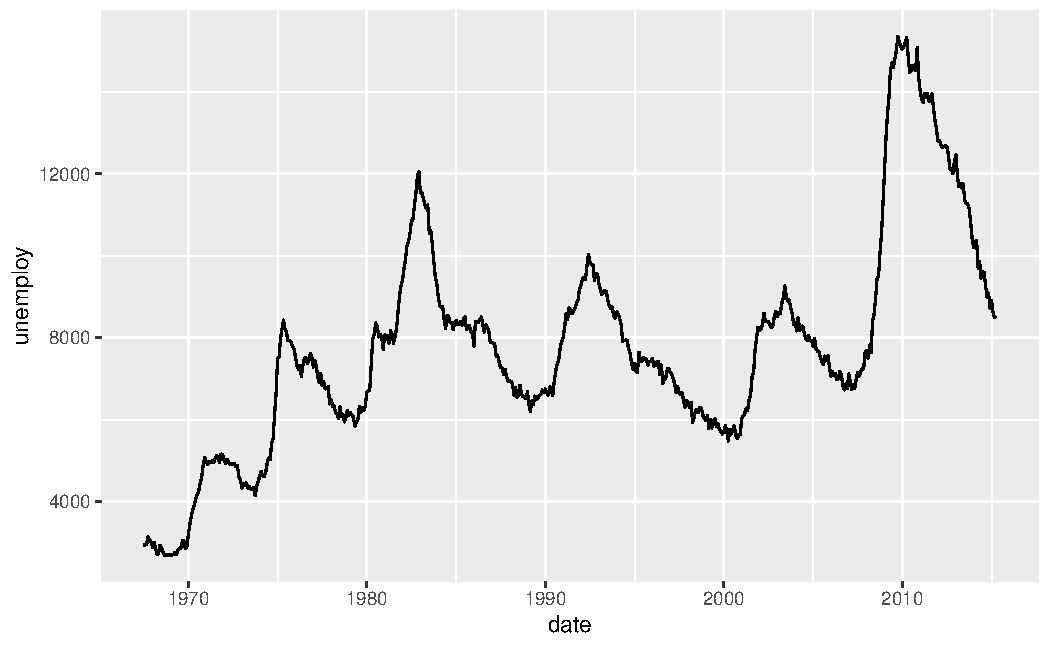
\includegraphics[width=1\linewidth]{mastering-r-through-errors_files/figure-latex/unnamed-chunk-1088-2} 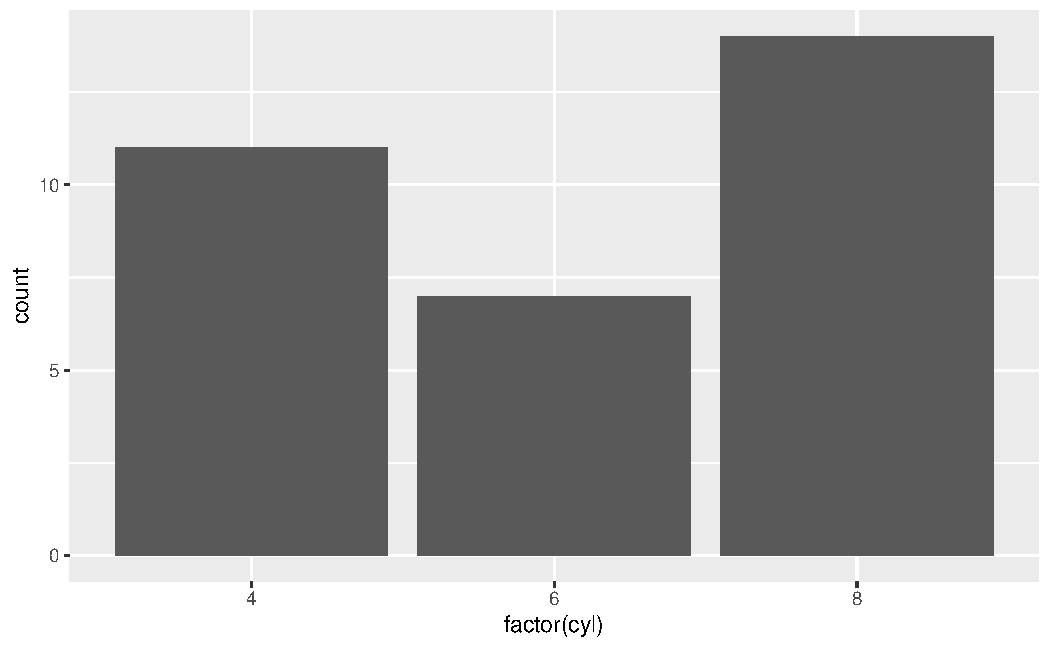
\includegraphics[width=1\linewidth]{mastering-r-through-errors_files/figure-latex/unnamed-chunk-1088-3} 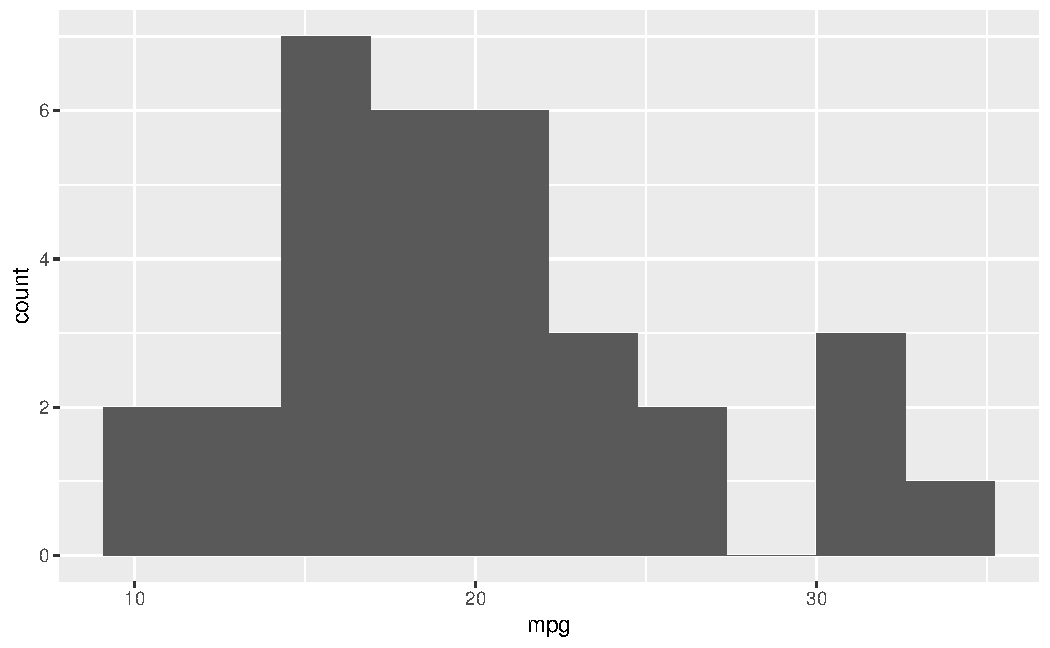
\includegraphics[width=1\linewidth]{mastering-r-through-errors_files/figure-latex/unnamed-chunk-1088-4} 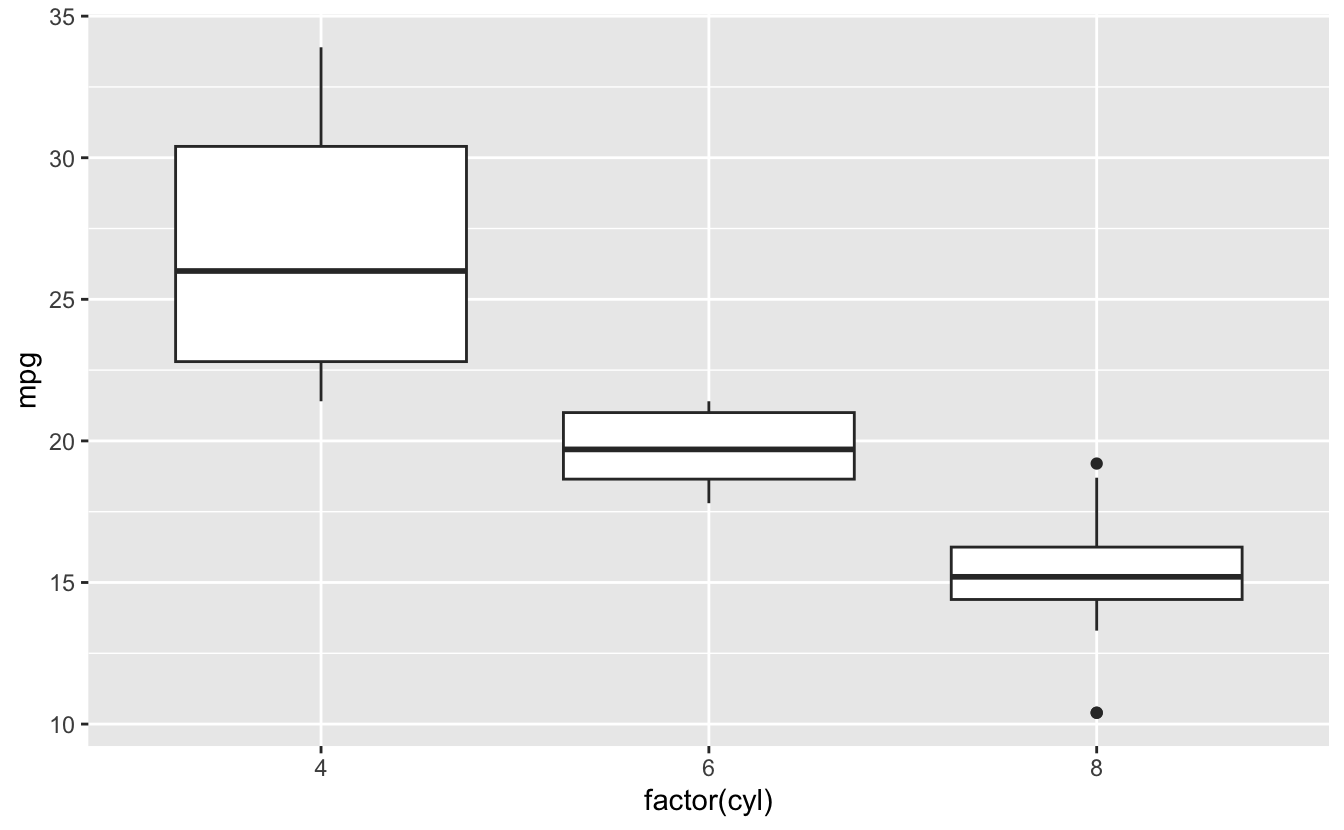
\includegraphics[width=1\linewidth]{mastering-r-through-errors_files/figure-latex/unnamed-chunk-1088-5} 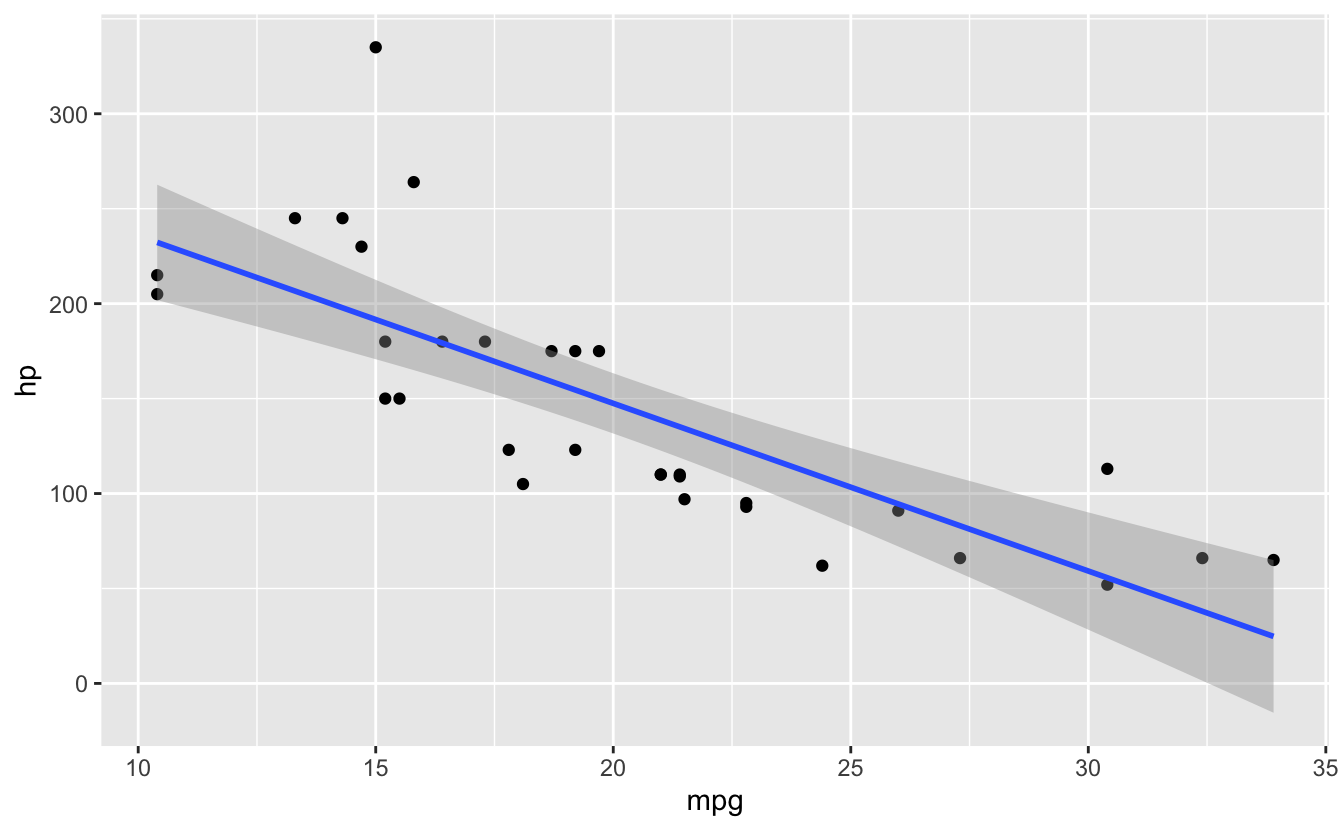
\includegraphics[width=1\linewidth]{mastering-r-through-errors_files/figure-latex/unnamed-chunk-1088-6} 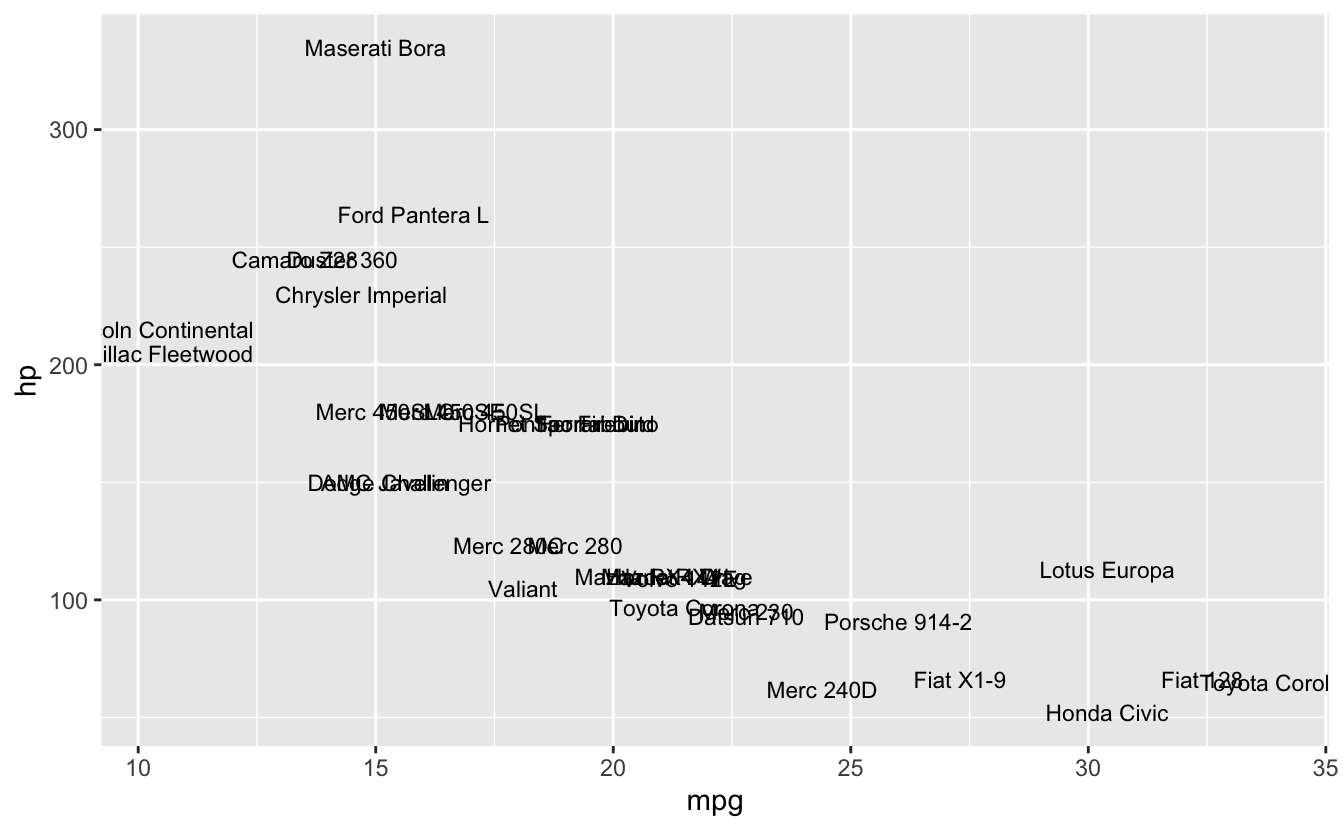
\includegraphics[width=1\linewidth]{mastering-r-through-errors_files/figure-latex/unnamed-chunk-1088-7} \end{center}

\section{\texorpdfstring{Error \#4: \texttt{stat\_count()\ requires\ x\ or\ y}}{Error \#4: stat\_count() requires x or y}}\label{stat-count-error}

{⭐ BEGINNER} {📋 ARGS}

\subsection{The Error}\label{the-error-83}

\begin{Shaded}
\begin{Highlighting}[]
\FunctionTok{ggplot}\NormalTok{(mtcars, }\FunctionTok{aes}\NormalTok{(}\AttributeTok{x =}\NormalTok{ mpg, }\AttributeTok{y =}\NormalTok{ hp)) }\SpecialCharTok{+}
  \FunctionTok{geom\_bar}\NormalTok{()}
\CommentTok{\#\textgreater{} Error in \textasciigrave{}geom\_bar()\textasciigrave{}:}
\CommentTok{\#\textgreater{} ! Problem while computing stat.}
\CommentTok{\#\textgreater{} i Error occurred in the 1st layer.}
\CommentTok{\#\textgreater{} Caused by error in \textasciigrave{}setup\_params()\textasciigrave{}:}
\CommentTok{\#\textgreater{} ! \textasciigrave{}stat\_count()\textasciigrave{} must only have an x or y aesthetic.}
\end{Highlighting}
\end{Shaded}

🔴 \textbf{ERROR}

\begin{verbatim}
Error in `geom_bar()`:
! Problem while computing stat.
ℹ Error occurred in the 1st layer.
Caused by error:
! `stat_count()` must only have an `x` or `y` aesthetic.
\end{verbatim}

\subsection{What It Means}\label{what-it-means-88}

\texttt{geom\_bar()} is for counts. For pre-computed heights, use \texttt{geom\_col()}.

\subsection{Solutions}\label{solutions-99}

✅ \textbf{SOLUTION 1: Use geom\_col() for Heights}

\begin{Shaded}
\begin{Highlighting}[]
\CommentTok{\# Pre{-}computed values}
\NormalTok{data }\OtherTok{\textless{}{-}} \FunctionTok{data.frame}\NormalTok{(}
  \AttributeTok{category =} \FunctionTok{c}\NormalTok{(}\StringTok{"A"}\NormalTok{, }\StringTok{"B"}\NormalTok{, }\StringTok{"C"}\NormalTok{),}
  \AttributeTok{value =} \FunctionTok{c}\NormalTok{(}\DecValTok{10}\NormalTok{, }\DecValTok{15}\NormalTok{, }\DecValTok{20}\NormalTok{)}
\NormalTok{)}

\FunctionTok{ggplot}\NormalTok{(data, }\FunctionTok{aes}\NormalTok{(}\AttributeTok{x =}\NormalTok{ category, }\AttributeTok{y =}\NormalTok{ value)) }\SpecialCharTok{+}
  \FunctionTok{geom\_col}\NormalTok{()}

\CommentTok{\# Or use stat = "identity" with geom\_bar}
\FunctionTok{ggplot}\NormalTok{(data, }\FunctionTok{aes}\NormalTok{(}\AttributeTok{x =}\NormalTok{ category, }\AttributeTok{y =}\NormalTok{ value)) }\SpecialCharTok{+}
  \FunctionTok{geom\_bar}\NormalTok{(}\AttributeTok{stat =} \StringTok{"identity"}\NormalTok{)}
\end{Highlighting}
\end{Shaded}

\begin{center}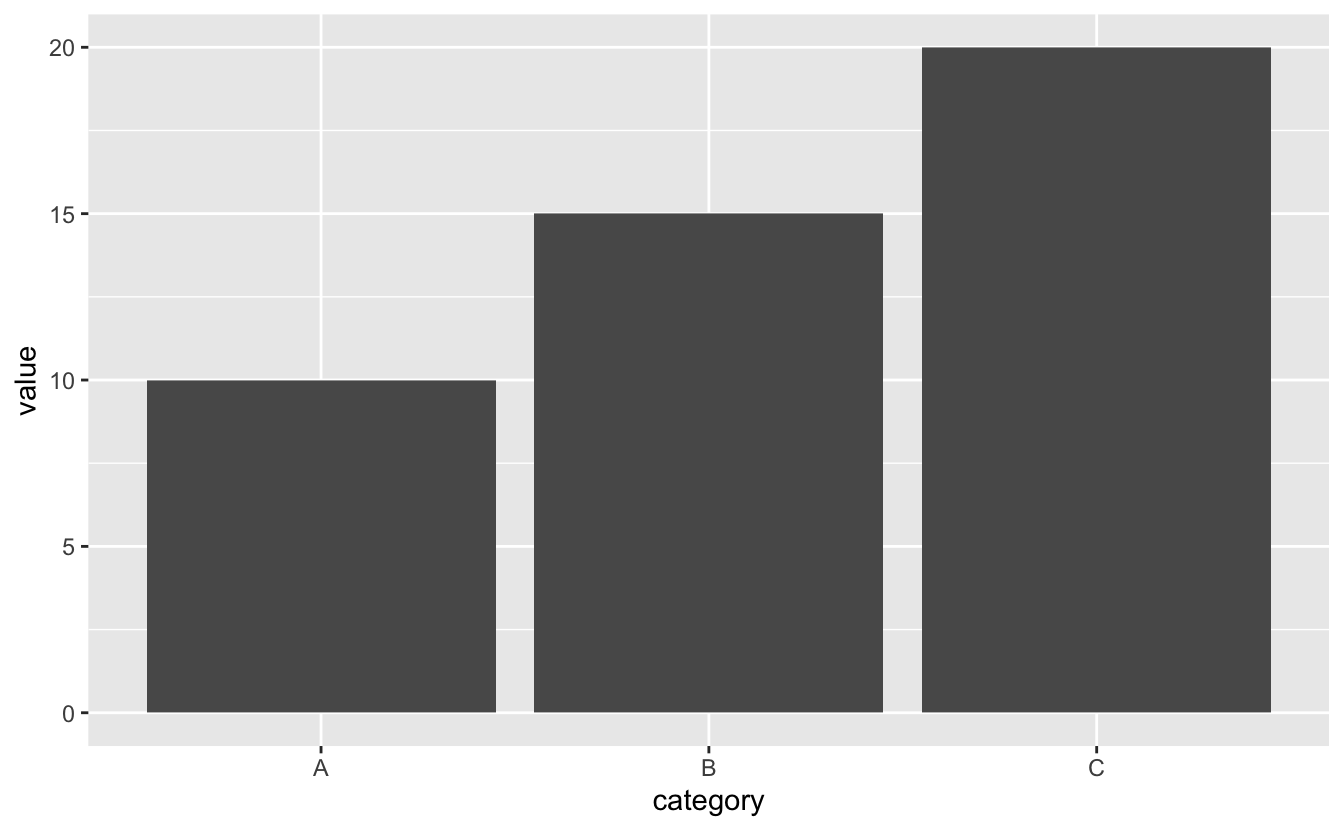
\includegraphics[width=1\linewidth]{mastering-r-through-errors_files/figure-latex/unnamed-chunk-1090-1} 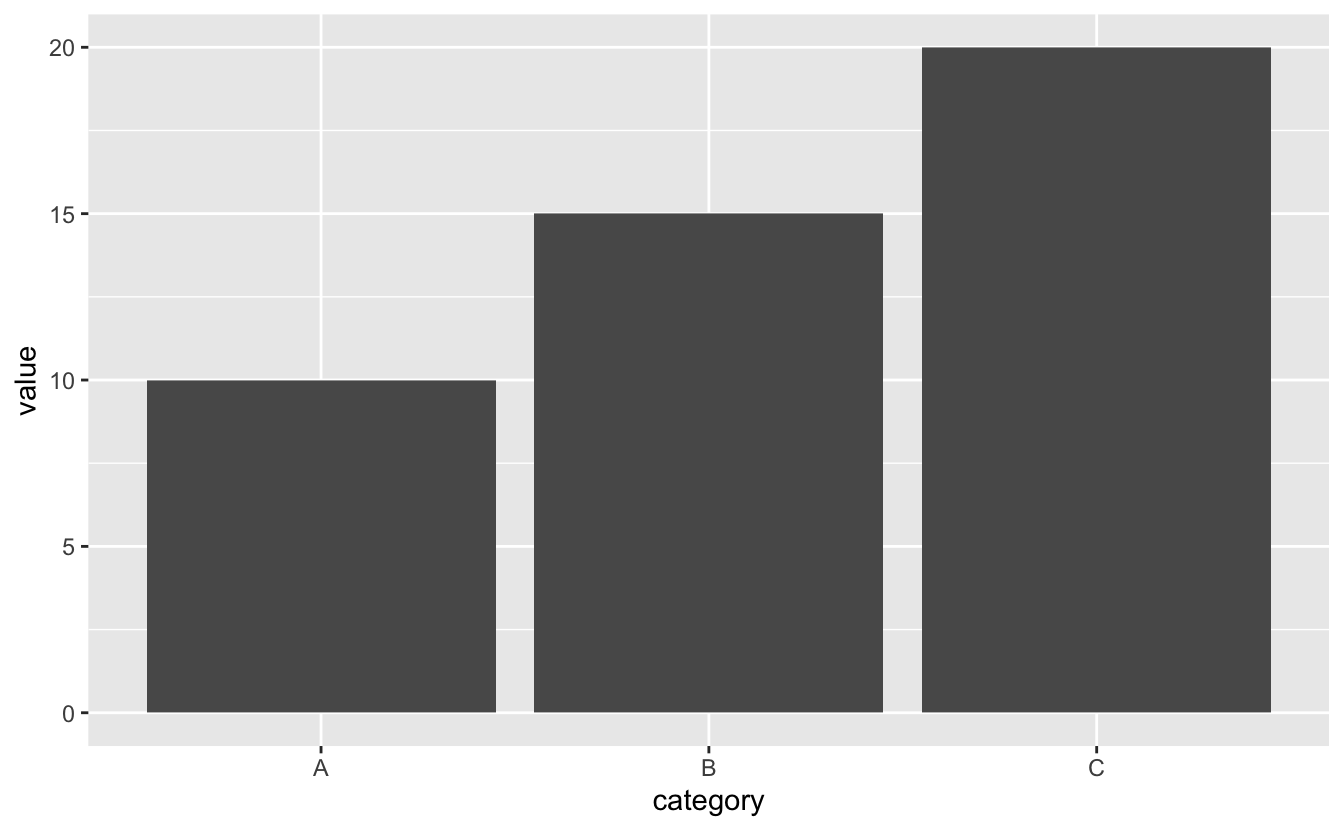
\includegraphics[width=1\linewidth]{mastering-r-through-errors_files/figure-latex/unnamed-chunk-1090-2} \end{center}

✅ \textbf{SOLUTION 2: Use geom\_bar() for Counts}

\begin{Shaded}
\begin{Highlighting}[]
\CommentTok{\# Count occurrences}
\FunctionTok{ggplot}\NormalTok{(mtcars, }\FunctionTok{aes}\NormalTok{(}\AttributeTok{x =} \FunctionTok{factor}\NormalTok{(cyl))) }\SpecialCharTok{+}
  \FunctionTok{geom\_bar}\NormalTok{()}

\CommentTok{\# Equivalent to}
\NormalTok{mtcars }\SpecialCharTok{\%\textgreater{}\%}
  \FunctionTok{count}\NormalTok{(cyl) }\SpecialCharTok{\%\textgreater{}\%}
  \FunctionTok{ggplot}\NormalTok{(}\FunctionTok{aes}\NormalTok{(}\AttributeTok{x =} \FunctionTok{factor}\NormalTok{(cyl), }\AttributeTok{y =}\NormalTok{ n)) }\SpecialCharTok{+}
  \FunctionTok{geom\_col}\NormalTok{()}
\end{Highlighting}
\end{Shaded}

\begin{center}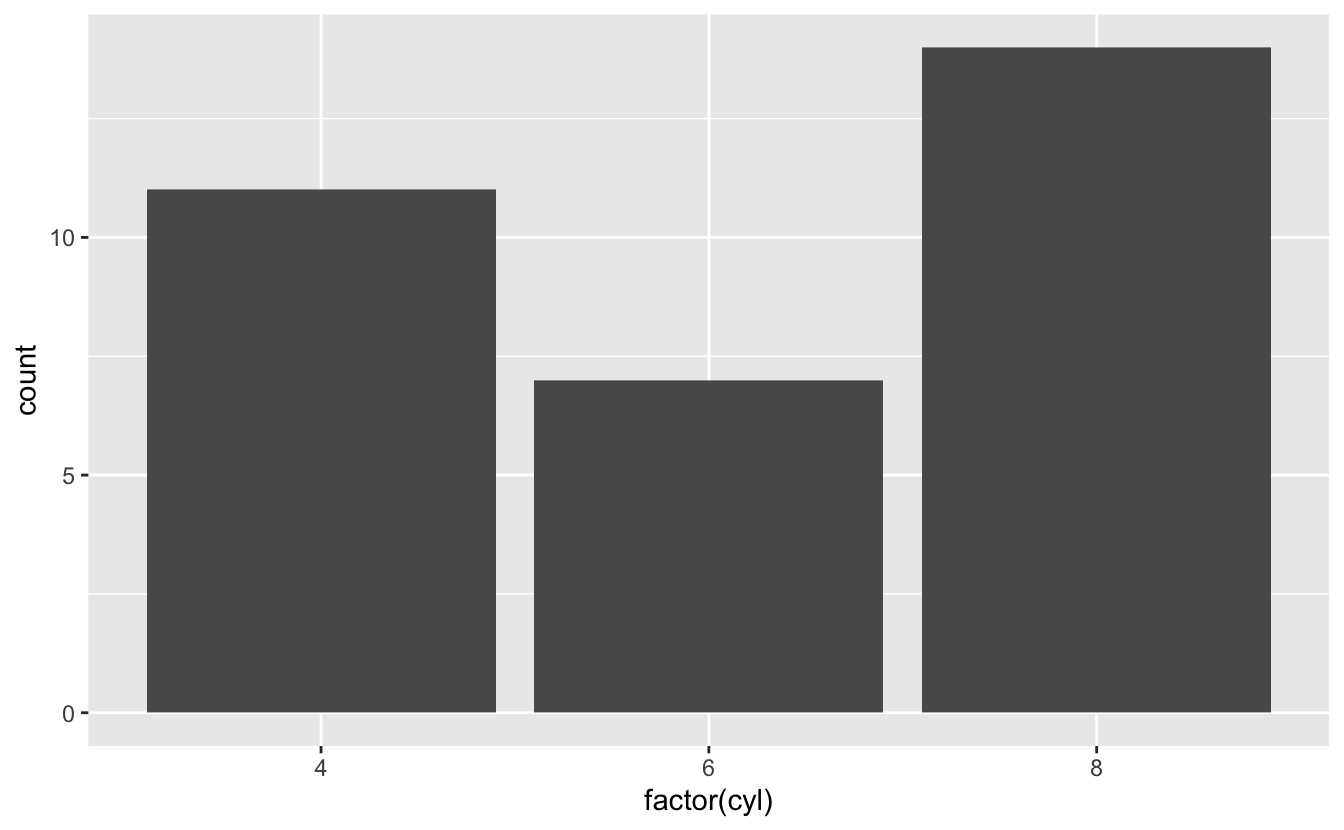
\includegraphics[width=1\linewidth]{mastering-r-through-errors_files/figure-latex/unnamed-chunk-1091-1} 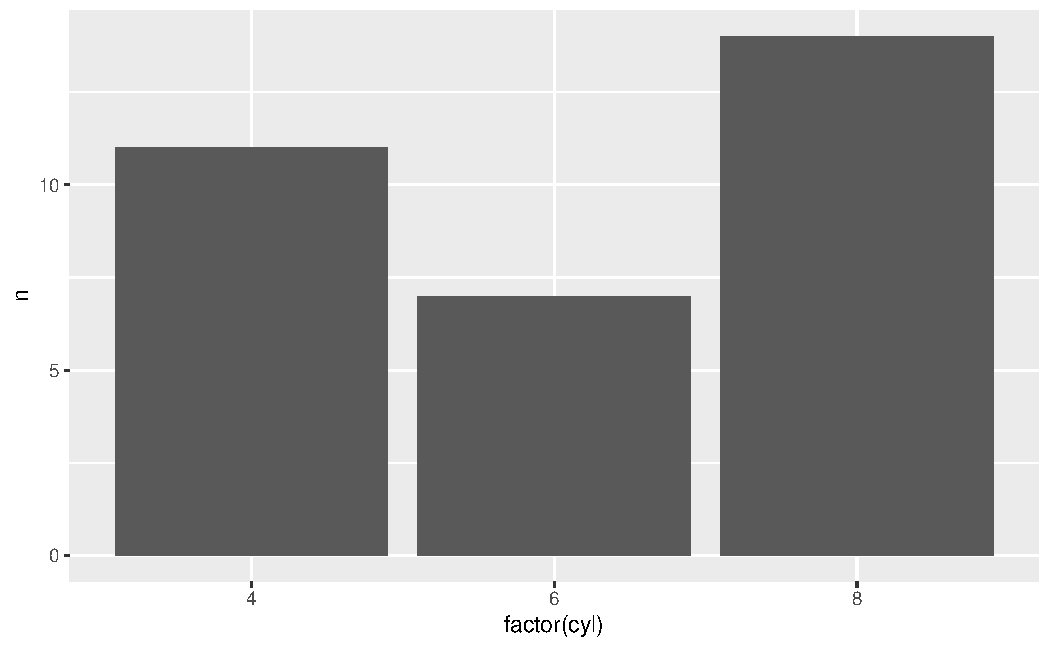
\includegraphics[width=1\linewidth]{mastering-r-through-errors_files/figure-latex/unnamed-chunk-1091-2} \end{center}

\section{Faceting}\label{faceting}

💡 \textbf{Key Insight: Small Multiples}

\begin{Shaded}
\begin{Highlighting}[]
\CommentTok{\# Facet by one variable}
\FunctionTok{ggplot}\NormalTok{(mtcars, }\FunctionTok{aes}\NormalTok{(}\AttributeTok{x =}\NormalTok{ mpg, }\AttributeTok{y =}\NormalTok{ hp)) }\SpecialCharTok{+}
  \FunctionTok{geom\_point}\NormalTok{() }\SpecialCharTok{+}
  \FunctionTok{facet\_wrap}\NormalTok{(}\SpecialCharTok{\textasciitilde{}}\NormalTok{ cyl)}

\CommentTok{\# Facet by two variables}
\FunctionTok{ggplot}\NormalTok{(mtcars, }\FunctionTok{aes}\NormalTok{(}\AttributeTok{x =}\NormalTok{ mpg, }\AttributeTok{y =}\NormalTok{ hp)) }\SpecialCharTok{+}
  \FunctionTok{geom\_point}\NormalTok{() }\SpecialCharTok{+}
  \FunctionTok{facet\_grid}\NormalTok{(cyl }\SpecialCharTok{\textasciitilde{}}\NormalTok{ gear)}

\CommentTok{\# Free scales}
\FunctionTok{ggplot}\NormalTok{(mtcars, }\FunctionTok{aes}\NormalTok{(}\AttributeTok{x =}\NormalTok{ mpg, }\AttributeTok{y =}\NormalTok{ hp)) }\SpecialCharTok{+}
  \FunctionTok{geom\_point}\NormalTok{() }\SpecialCharTok{+}
  \FunctionTok{facet\_wrap}\NormalTok{(}\SpecialCharTok{\textasciitilde{}}\NormalTok{ cyl, }\AttributeTok{scales =} \StringTok{"free"}\NormalTok{)}

\CommentTok{\# Number of columns}
\FunctionTok{ggplot}\NormalTok{(mtcars, }\FunctionTok{aes}\NormalTok{(}\AttributeTok{x =}\NormalTok{ mpg, }\AttributeTok{y =}\NormalTok{ hp)) }\SpecialCharTok{+}
  \FunctionTok{geom\_point}\NormalTok{() }\SpecialCharTok{+}
  \FunctionTok{facet\_wrap}\NormalTok{(}\SpecialCharTok{\textasciitilde{}}\NormalTok{ cyl, }\AttributeTok{ncol =} \DecValTok{2}\NormalTok{)}
\end{Highlighting}
\end{Shaded}

\begin{center}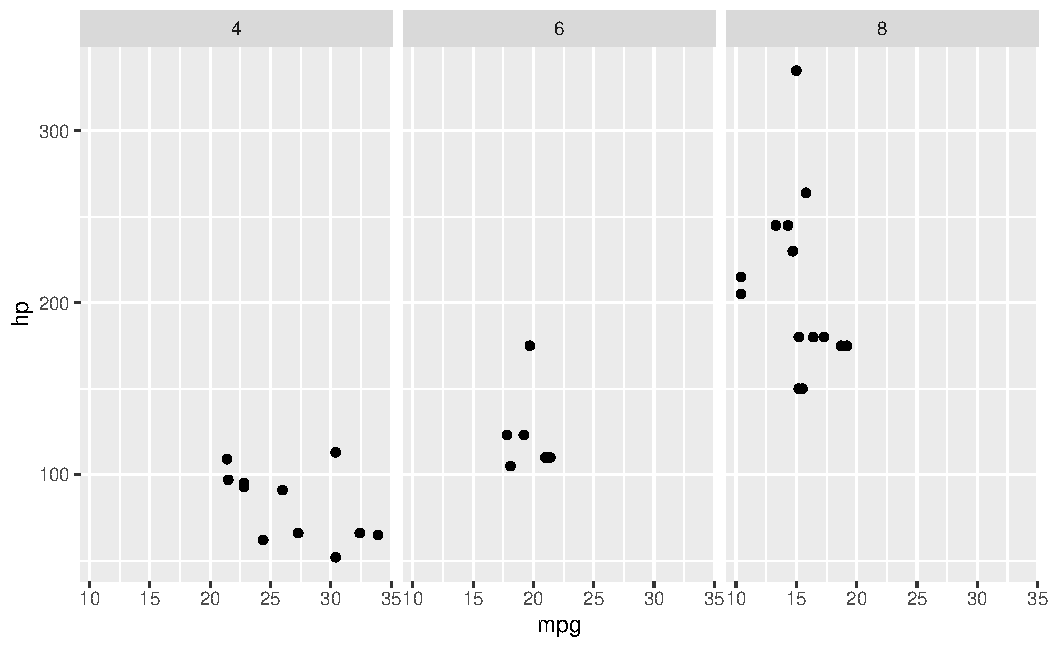
\includegraphics[width=1\linewidth]{mastering-r-through-errors_files/figure-latex/unnamed-chunk-1092-1} 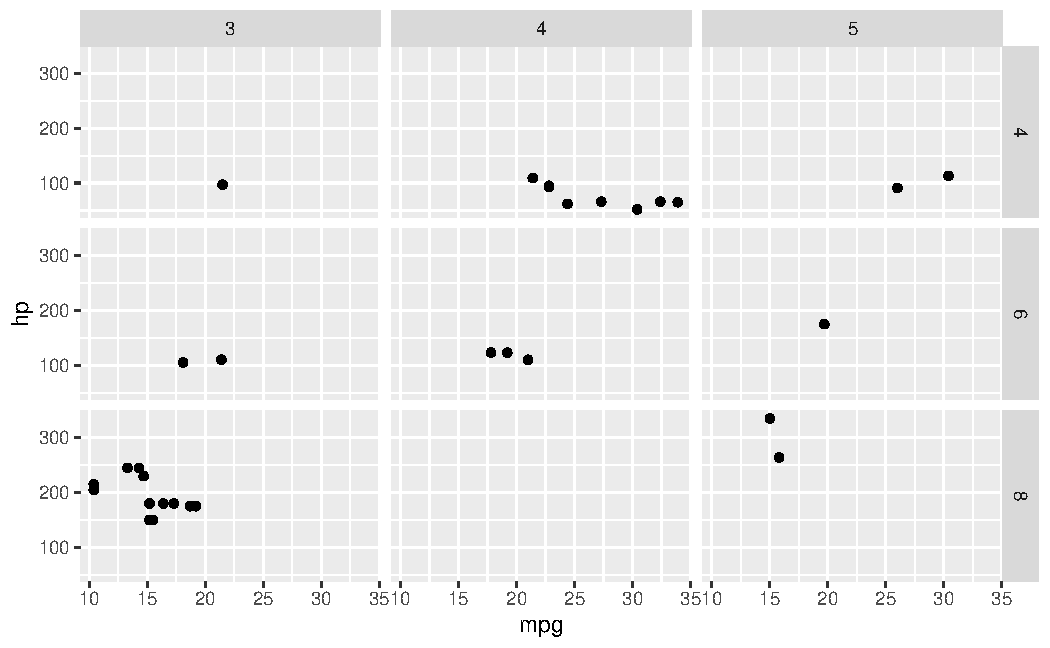
\includegraphics[width=1\linewidth]{mastering-r-through-errors_files/figure-latex/unnamed-chunk-1092-2} 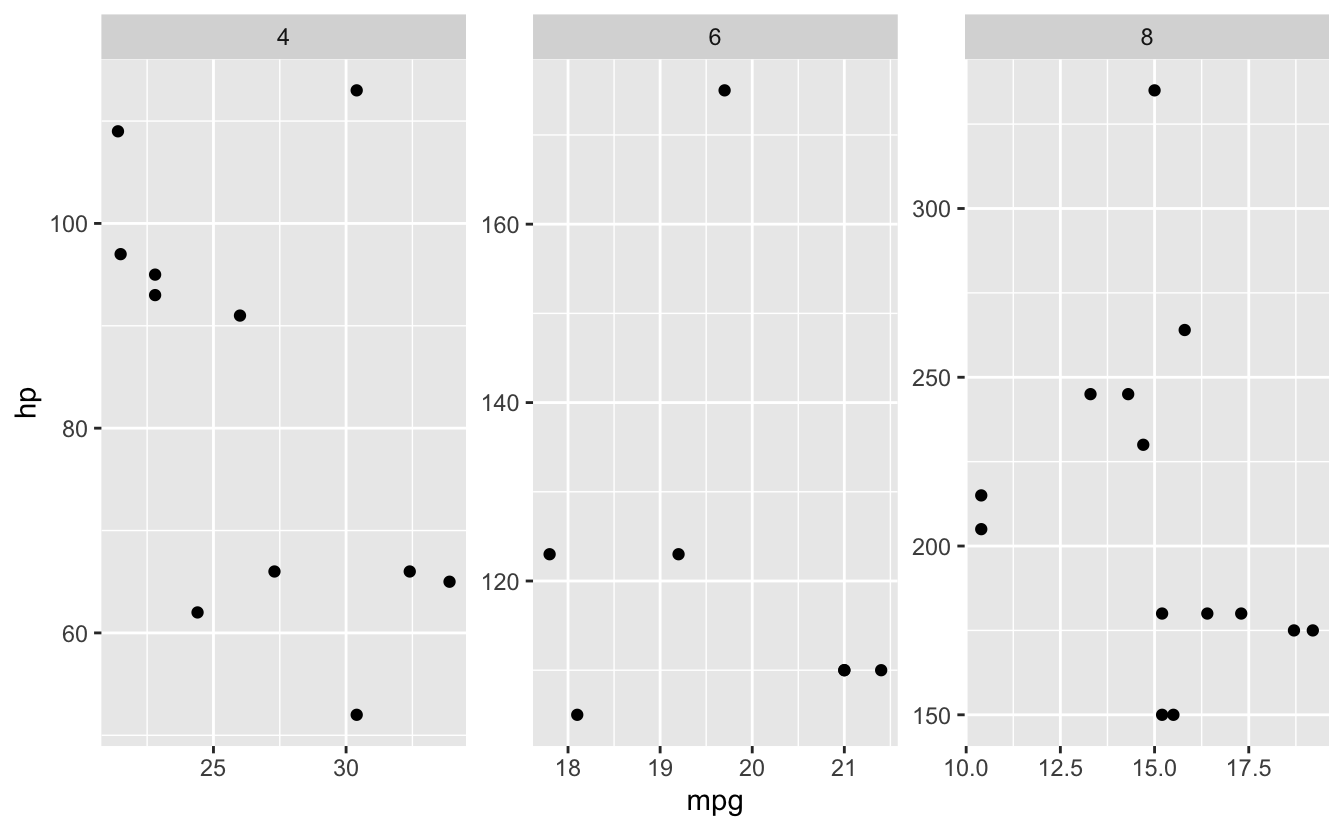
\includegraphics[width=1\linewidth]{mastering-r-through-errors_files/figure-latex/unnamed-chunk-1092-3} 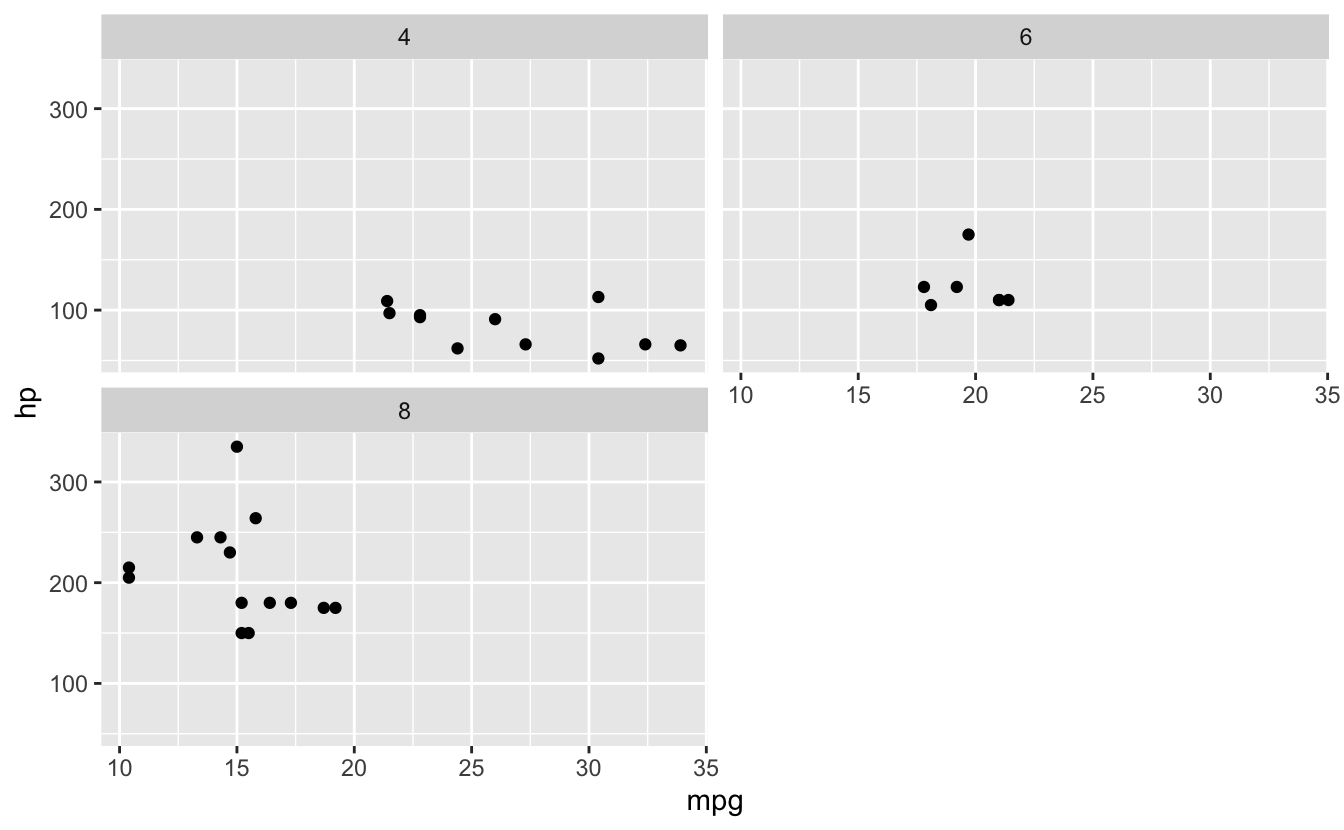
\includegraphics[width=1\linewidth]{mastering-r-through-errors_files/figure-latex/unnamed-chunk-1092-4} \end{center}

\section{Themes and Customization}\label{themes-and-customization}

🎯 \textbf{Best Practice: Customizing Plots}

\begin{Shaded}
\begin{Highlighting}[]
\CommentTok{\# Built{-}in themes}
\NormalTok{p }\OtherTok{\textless{}{-}} \FunctionTok{ggplot}\NormalTok{(mtcars, }\FunctionTok{aes}\NormalTok{(}\AttributeTok{x =}\NormalTok{ mpg, }\AttributeTok{y =}\NormalTok{ hp)) }\SpecialCharTok{+}
  \FunctionTok{geom\_point}\NormalTok{()}

\NormalTok{p }\SpecialCharTok{+} \FunctionTok{theme\_minimal}\NormalTok{()}
\NormalTok{p }\SpecialCharTok{+} \FunctionTok{theme\_classic}\NormalTok{()}
\NormalTok{p }\SpecialCharTok{+} \FunctionTok{theme\_bw}\NormalTok{()}

\CommentTok{\# Custom labels}
\FunctionTok{ggplot}\NormalTok{(mtcars, }\FunctionTok{aes}\NormalTok{(}\AttributeTok{x =}\NormalTok{ mpg, }\AttributeTok{y =}\NormalTok{ hp)) }\SpecialCharTok{+}
  \FunctionTok{geom\_point}\NormalTok{() }\SpecialCharTok{+}
  \FunctionTok{labs}\NormalTok{(}
    \AttributeTok{title =} \StringTok{"Fuel Efficiency vs Horsepower"}\NormalTok{,}
    \AttributeTok{subtitle =} \StringTok{"Motor Trend Car Road Tests"}\NormalTok{,}
    \AttributeTok{x =} \StringTok{"Miles per Gallon"}\NormalTok{,}
    \AttributeTok{y =} \StringTok{"Horsepower"}\NormalTok{,}
    \AttributeTok{caption =} \StringTok{"Source: mtcars dataset"}
\NormalTok{  )}

\CommentTok{\# Customize theme elements}
\FunctionTok{ggplot}\NormalTok{(mtcars, }\FunctionTok{aes}\NormalTok{(}\AttributeTok{x =}\NormalTok{ mpg, }\AttributeTok{y =}\NormalTok{ hp)) }\SpecialCharTok{+}
  \FunctionTok{geom\_point}\NormalTok{() }\SpecialCharTok{+}
  \FunctionTok{theme\_minimal}\NormalTok{() }\SpecialCharTok{+}
  \FunctionTok{theme}\NormalTok{(}
    \AttributeTok{plot.title =} \FunctionTok{element\_text}\NormalTok{(}\AttributeTok{face =} \StringTok{"bold"}\NormalTok{, }\AttributeTok{size =} \DecValTok{14}\NormalTok{),}
    \AttributeTok{axis.text =} \FunctionTok{element\_text}\NormalTok{(}\AttributeTok{size =} \DecValTok{10}\NormalTok{),}
    \AttributeTok{panel.grid.minor =} \FunctionTok{element\_blank}\NormalTok{()}
\NormalTok{  )}
\end{Highlighting}
\end{Shaded}

\begin{center}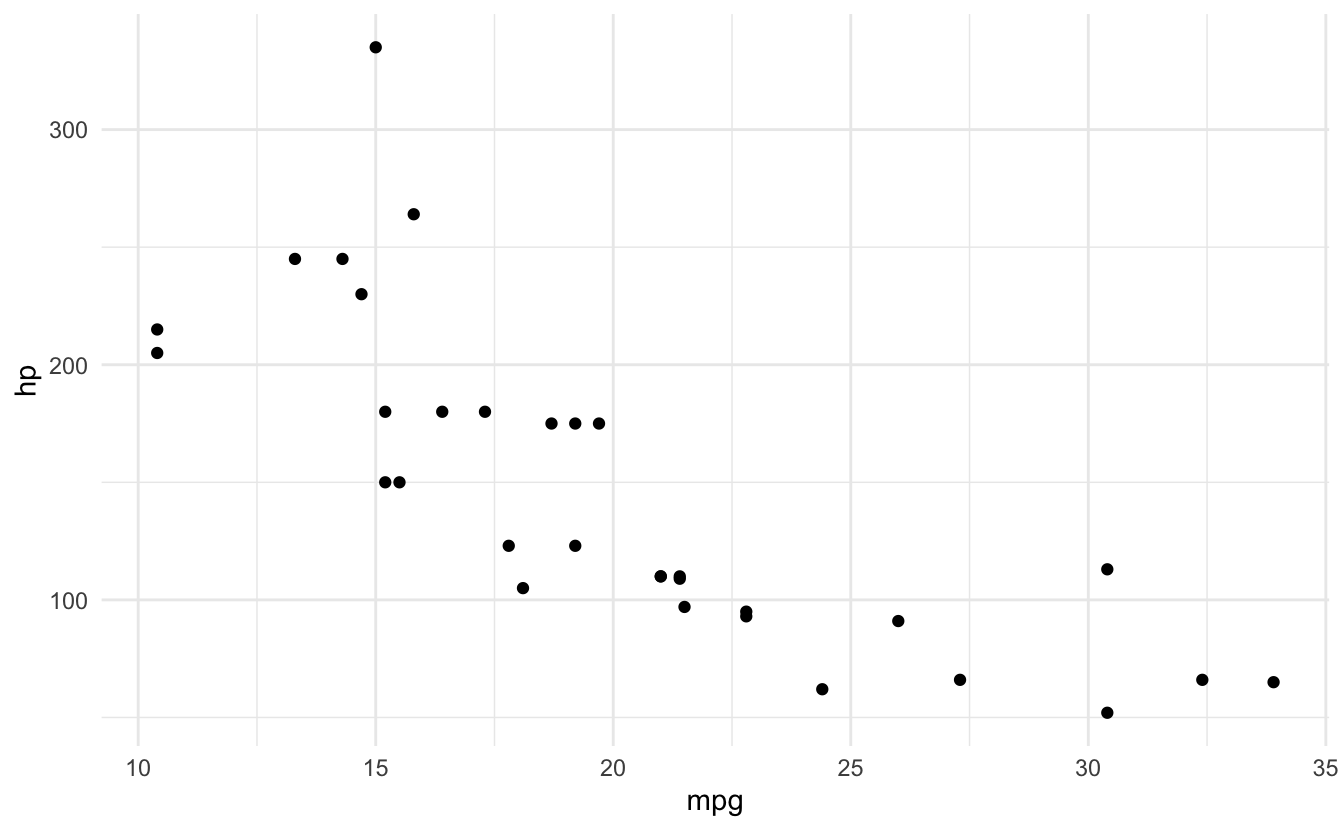
\includegraphics[width=1\linewidth]{mastering-r-through-errors_files/figure-latex/unnamed-chunk-1093-1} 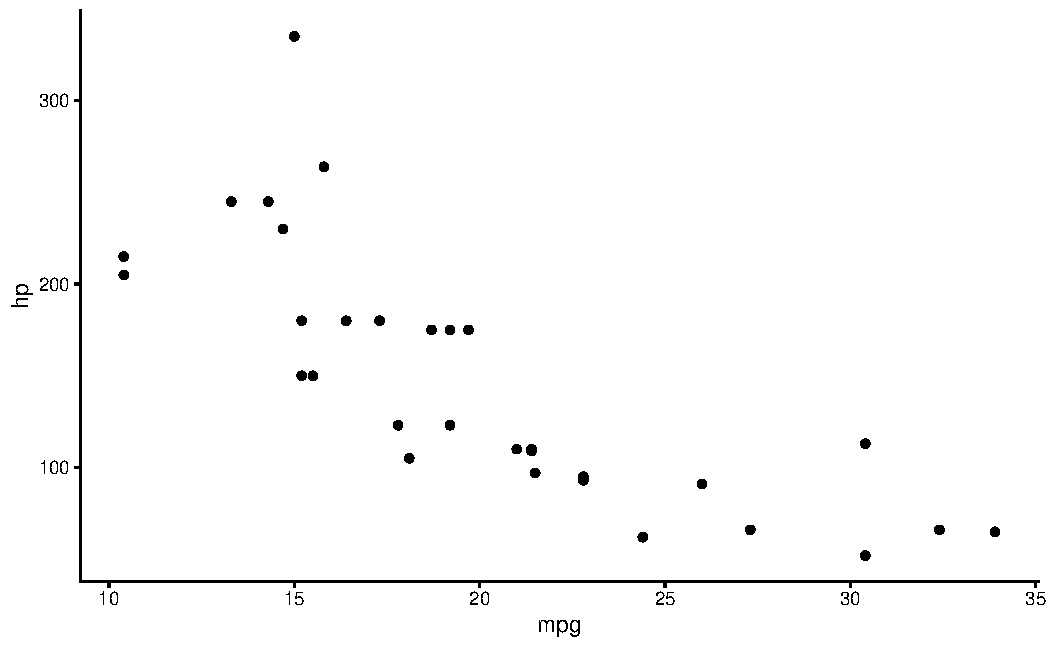
\includegraphics[width=1\linewidth]{mastering-r-through-errors_files/figure-latex/unnamed-chunk-1093-2} 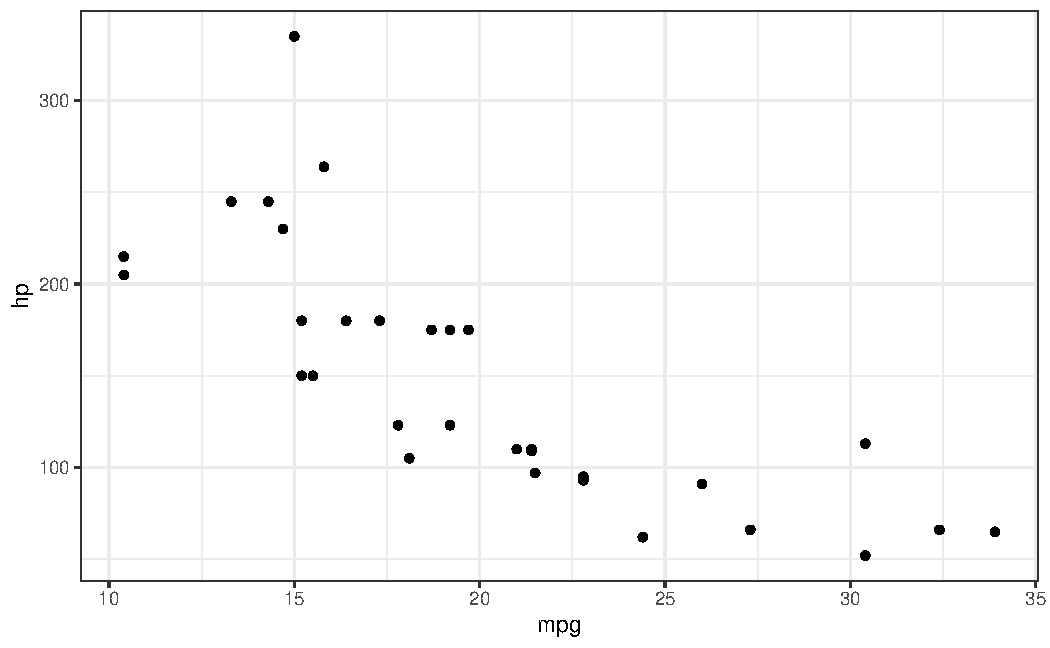
\includegraphics[width=1\linewidth]{mastering-r-through-errors_files/figure-latex/unnamed-chunk-1093-3} 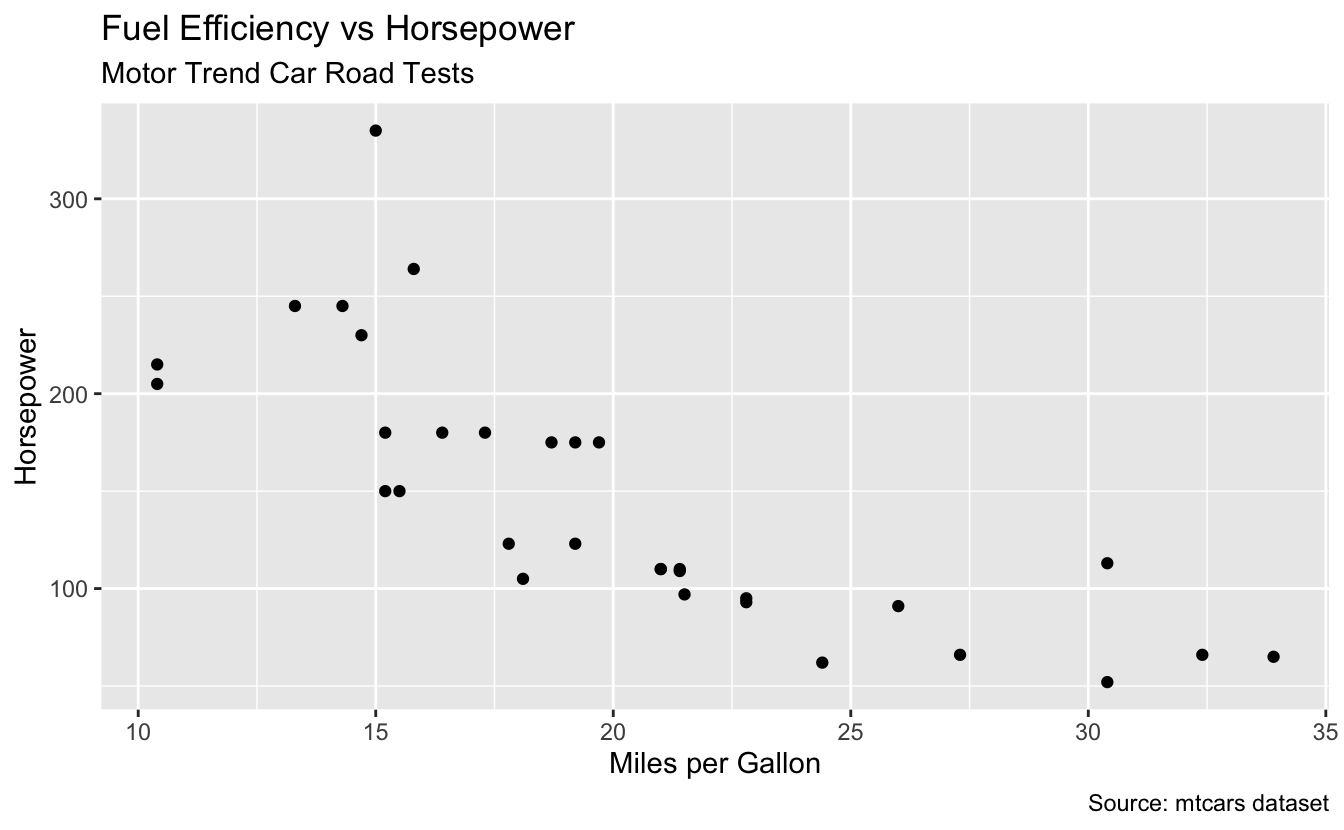
\includegraphics[width=1\linewidth]{mastering-r-through-errors_files/figure-latex/unnamed-chunk-1093-4} 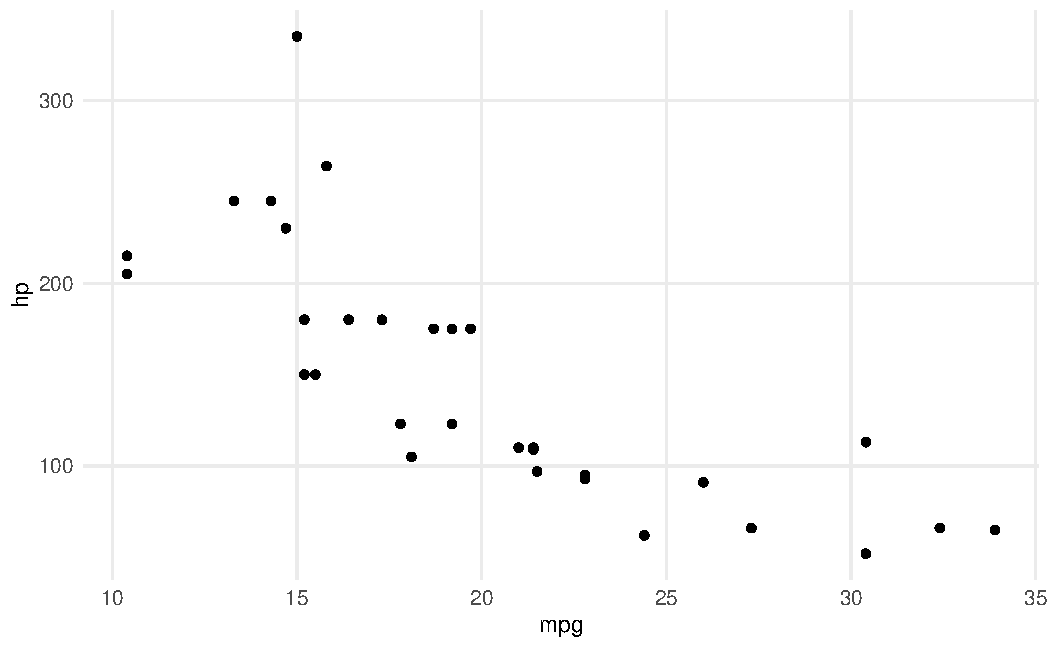
\includegraphics[width=1\linewidth]{mastering-r-through-errors_files/figure-latex/unnamed-chunk-1093-5} \end{center}

\section{Error \#5: Non-numeric variable for histogram}\label{histogram-non-numeric}

{⭐ BEGINNER} {🔢 TYPE}

\subsection{The Error}\label{the-error-84}

\begin{Shaded}
\begin{Highlighting}[]
\FunctionTok{ggplot}\NormalTok{(mtcars, }\FunctionTok{aes}\NormalTok{(}\AttributeTok{x =} \FunctionTok{factor}\NormalTok{(cyl))) }\SpecialCharTok{+}
  \FunctionTok{geom\_histogram}\NormalTok{()}
\CommentTok{\#\textgreater{} Error in \textasciigrave{}geom\_histogram()\textasciigrave{}:}
\CommentTok{\#\textgreater{} ! Problem while computing stat.}
\CommentTok{\#\textgreater{} i Error occurred in the 1st layer.}
\CommentTok{\#\textgreater{} Caused by error in \textasciigrave{}setup\_params()\textasciigrave{}:}
\CommentTok{\#\textgreater{} ! \textasciigrave{}stat\_bin()\textasciigrave{} requires a continuous x aesthetic.}
\CommentTok{\#\textgreater{} x the x aesthetic is discrete.}
\CommentTok{\#\textgreater{} i Perhaps you want \textasciigrave{}stat="count"\textasciigrave{}?}
\end{Highlighting}
\end{Shaded}

🔴 \textbf{ERROR}

\begin{verbatim}
Error in `geom_histogram()`:
! `stat_bin()` requires a numeric `x` variable
\end{verbatim}

\subsection{What It Means}\label{what-it-means-89}

Histograms need continuous numeric data, not categorical.

\subsection{Solutions}\label{solutions-100}

✅ \textbf{SOLUTION: Use Appropriate Geom}

\begin{Shaded}
\begin{Highlighting}[]
\CommentTok{\# For categorical: use geom\_bar}
\FunctionTok{ggplot}\NormalTok{(mtcars, }\FunctionTok{aes}\NormalTok{(}\AttributeTok{x =} \FunctionTok{factor}\NormalTok{(cyl))) }\SpecialCharTok{+}
  \FunctionTok{geom\_bar}\NormalTok{()}

\CommentTok{\# For continuous: histogram works}
\FunctionTok{ggplot}\NormalTok{(mtcars, }\FunctionTok{aes}\NormalTok{(}\AttributeTok{x =}\NormalTok{ mpg)) }\SpecialCharTok{+}
  \FunctionTok{geom\_histogram}\NormalTok{(}\AttributeTok{bins =} \DecValTok{10}\NormalTok{)}

\CommentTok{\# Density plot alternative}
\FunctionTok{ggplot}\NormalTok{(mtcars, }\FunctionTok{aes}\NormalTok{(}\AttributeTok{x =}\NormalTok{ mpg)) }\SpecialCharTok{+}
  \FunctionTok{geom\_density}\NormalTok{()}
\end{Highlighting}
\end{Shaded}

\begin{center}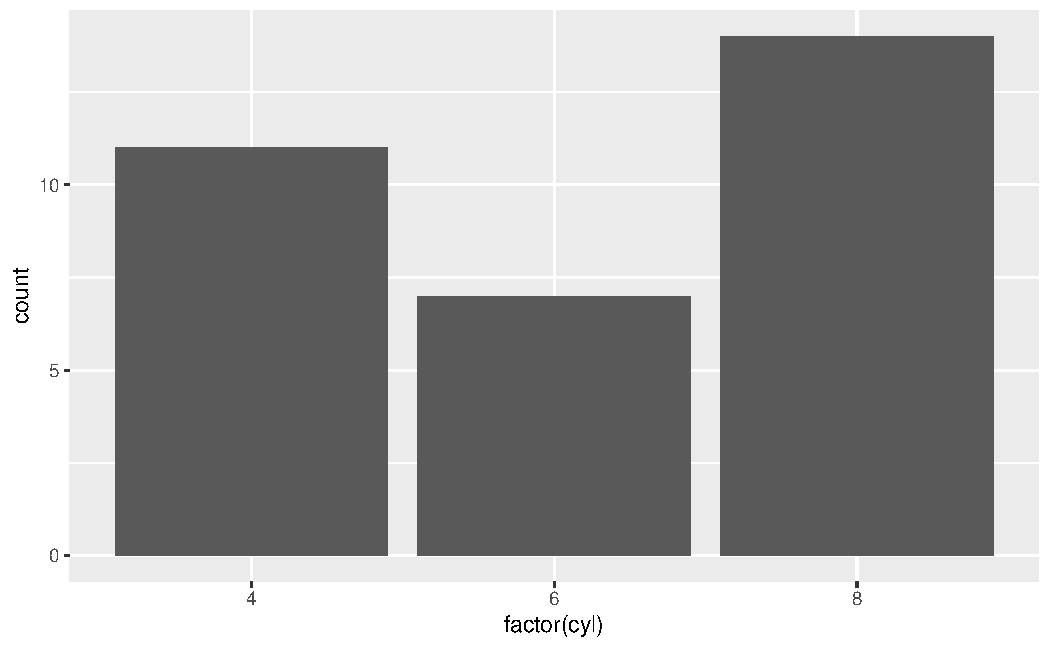
\includegraphics[width=1\linewidth]{mastering-r-through-errors_files/figure-latex/unnamed-chunk-1095-1} 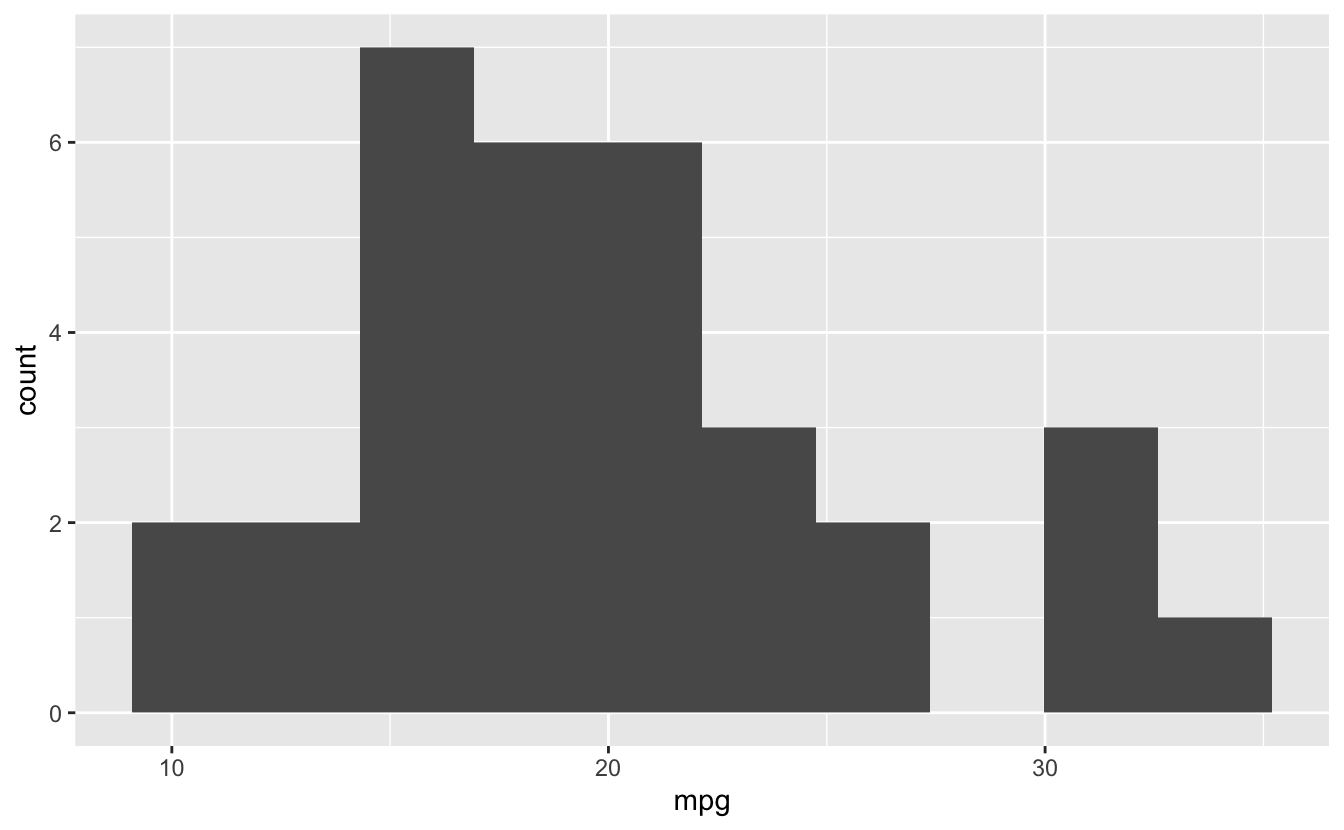
\includegraphics[width=1\linewidth]{mastering-r-through-errors_files/figure-latex/unnamed-chunk-1095-2} 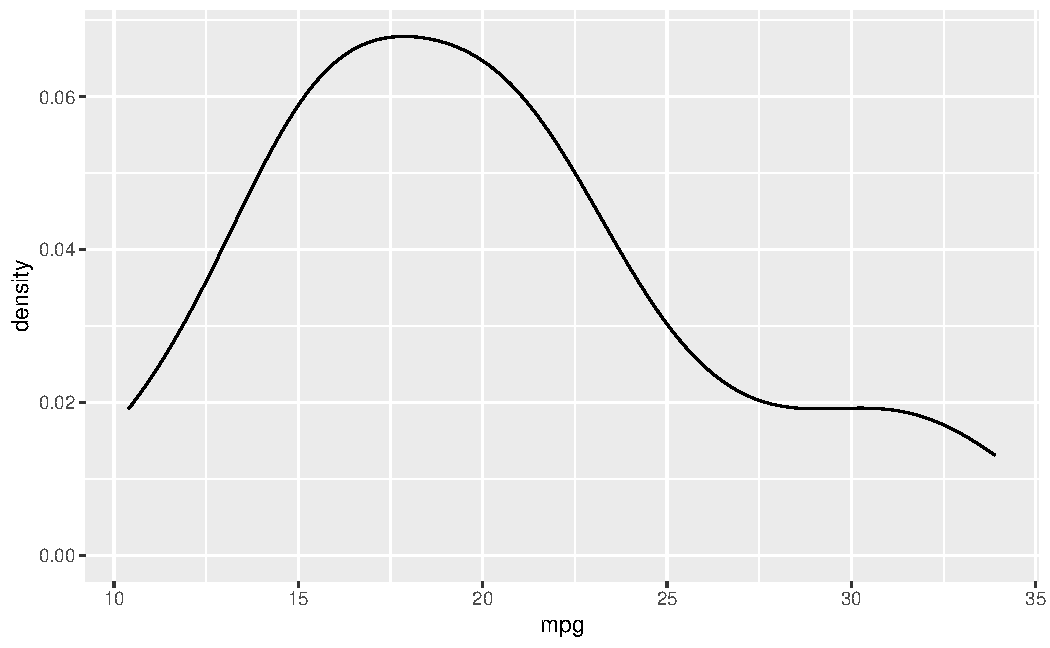
\includegraphics[width=1\linewidth]{mastering-r-through-errors_files/figure-latex/unnamed-chunk-1095-3} \end{center}

\section{Saving Plots}\label{saving-plots}

🎯 \textbf{Best Practice: Save Plots}

\begin{Shaded}
\begin{Highlighting}[]
\CommentTok{\# Create plot}
\NormalTok{p }\OtherTok{\textless{}{-}} \FunctionTok{ggplot}\NormalTok{(mtcars, }\FunctionTok{aes}\NormalTok{(}\AttributeTok{x =}\NormalTok{ mpg, }\AttributeTok{y =}\NormalTok{ hp)) }\SpecialCharTok{+}
  \FunctionTok{geom\_point}\NormalTok{() }\SpecialCharTok{+}
  \FunctionTok{theme\_minimal}\NormalTok{()}

\CommentTok{\# Save with ggsave}
\FunctionTok{ggsave}\NormalTok{(}\StringTok{"plot.png"}\NormalTok{, p, }\AttributeTok{width =} \DecValTok{6}\NormalTok{, }\AttributeTok{height =} \DecValTok{4}\NormalTok{, }\AttributeTok{dpi =} \DecValTok{300}\NormalTok{)}

\CommentTok{\# Or save last plot}
\FunctionTok{ggplot}\NormalTok{(mtcars, }\FunctionTok{aes}\NormalTok{(}\AttributeTok{x =}\NormalTok{ mpg, }\AttributeTok{y =}\NormalTok{ hp)) }\SpecialCharTok{+}
  \FunctionTok{geom\_point}\NormalTok{()}

\FunctionTok{ggsave}\NormalTok{(}\StringTok{"last\_plot.png"}\NormalTok{, }\AttributeTok{width =} \DecValTok{6}\NormalTok{, }\AttributeTok{height =} \DecValTok{4}\NormalTok{)}

\CommentTok{\# Different formats}
\FunctionTok{ggsave}\NormalTok{(}\StringTok{"plot.pdf"}\NormalTok{, p)}
\FunctionTok{ggsave}\NormalTok{(}\StringTok{"plot.svg"}\NormalTok{, p)}
\FunctionTok{ggsave}\NormalTok{(}\StringTok{"plot.jpg"}\NormalTok{, p)}
\end{Highlighting}
\end{Shaded}

\section{Common Patterns}\label{common-patterns-2}

🎯 \textbf{Best Practice: Common Plot Types}

\begin{Shaded}
\begin{Highlighting}[]
\CommentTok{\# Scatterplot with trend line}
\FunctionTok{ggplot}\NormalTok{(mtcars, }\FunctionTok{aes}\NormalTok{(}\AttributeTok{x =}\NormalTok{ mpg, }\AttributeTok{y =}\NormalTok{ hp)) }\SpecialCharTok{+}
  \FunctionTok{geom\_point}\NormalTok{(}\FunctionTok{aes}\NormalTok{(}\AttributeTok{color =} \FunctionTok{factor}\NormalTok{(cyl))) }\SpecialCharTok{+}
  \FunctionTok{geom\_smooth}\NormalTok{(}\AttributeTok{method =} \StringTok{"lm"}\NormalTok{, }\AttributeTok{se =} \ConstantTok{FALSE}\NormalTok{) }\SpecialCharTok{+}
  \FunctionTok{theme\_minimal}\NormalTok{()}
\CommentTok{\#\textgreater{} \textasciigrave{}geom\_smooth()\textasciigrave{} using formula = \textquotesingle{}y \textasciitilde{} x\textquotesingle{}}

\CommentTok{\# Grouped bar chart}
\NormalTok{mtcars }\SpecialCharTok{\%\textgreater{}\%}
  \FunctionTok{count}\NormalTok{(cyl, gear) }\SpecialCharTok{\%\textgreater{}\%}
  \FunctionTok{ggplot}\NormalTok{(}\FunctionTok{aes}\NormalTok{(}\AttributeTok{x =} \FunctionTok{factor}\NormalTok{(cyl), }\AttributeTok{y =}\NormalTok{ n, }\AttributeTok{fill =} \FunctionTok{factor}\NormalTok{(gear))) }\SpecialCharTok{+}
  \FunctionTok{geom\_col}\NormalTok{(}\AttributeTok{position =} \StringTok{"dodge"}\NormalTok{)}

\CommentTok{\# Boxplot with points}
\FunctionTok{ggplot}\NormalTok{(mtcars, }\FunctionTok{aes}\NormalTok{(}\AttributeTok{x =} \FunctionTok{factor}\NormalTok{(cyl), }\AttributeTok{y =}\NormalTok{ mpg)) }\SpecialCharTok{+}
  \FunctionTok{geom\_boxplot}\NormalTok{() }\SpecialCharTok{+}
  \FunctionTok{geom\_jitter}\NormalTok{(}\AttributeTok{width =} \FloatTok{0.2}\NormalTok{, }\AttributeTok{alpha =} \FloatTok{0.3}\NormalTok{)}

\CommentTok{\# Time series}
\FunctionTok{ggplot}\NormalTok{(economics, }\FunctionTok{aes}\NormalTok{(}\AttributeTok{x =}\NormalTok{ date, }\AttributeTok{y =}\NormalTok{ unemploy)) }\SpecialCharTok{+}
  \FunctionTok{geom\_line}\NormalTok{() }\SpecialCharTok{+}
  \FunctionTok{theme\_minimal}\NormalTok{() }\SpecialCharTok{+}
  \FunctionTok{labs}\NormalTok{(}\AttributeTok{title =} \StringTok{"US Unemployment Over Time"}\NormalTok{)}
\end{Highlighting}
\end{Shaded}

\begin{center}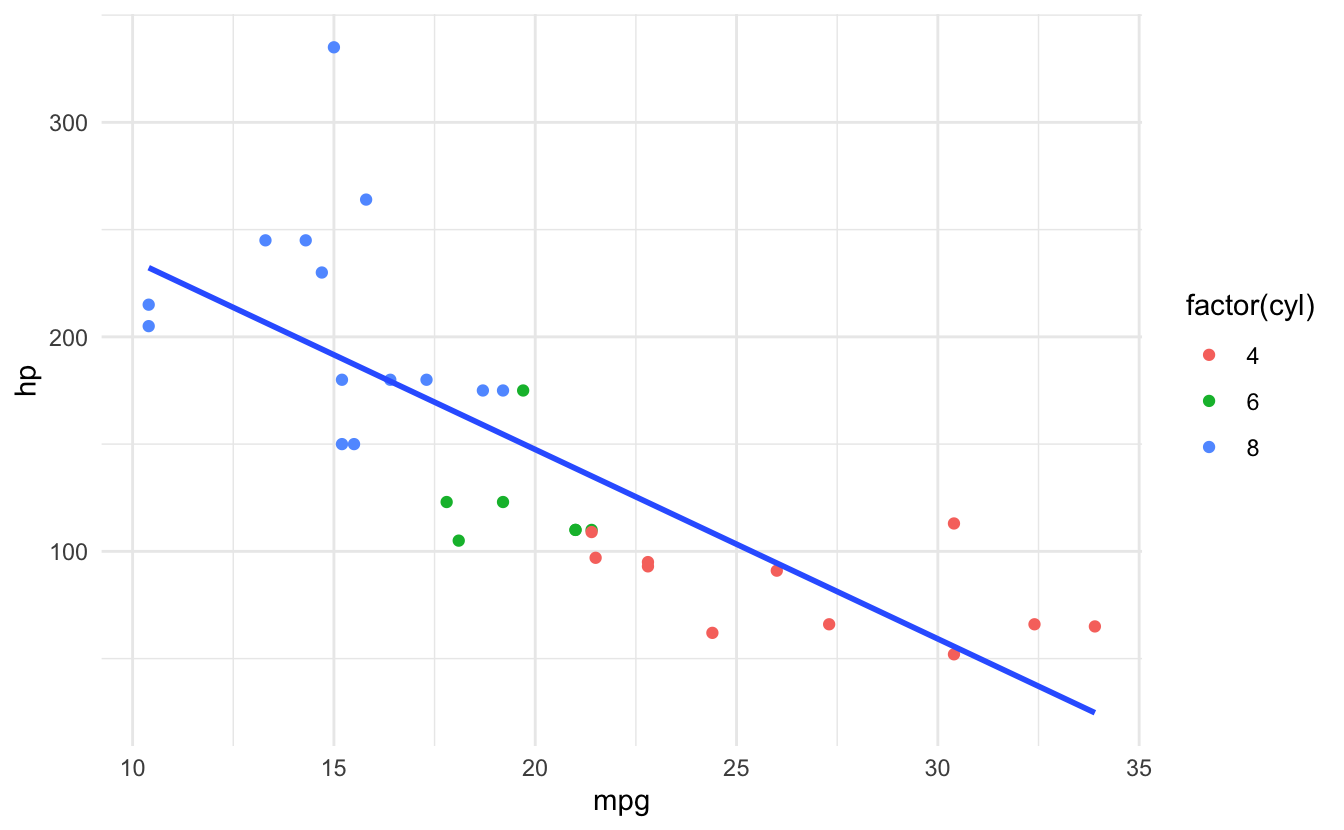
\includegraphics[width=1\linewidth]{mastering-r-through-errors_files/figure-latex/unnamed-chunk-1097-1} \includegraphics[width=1\linewidth]{mastering-r-through-errors_files/figure-latex/unnamed-chunk-1097-2} \includegraphics[width=1\linewidth]{mastering-r-through-errors_files/figure-latex/unnamed-chunk-1097-3} \includegraphics[width=1\linewidth]{mastering-r-through-errors_files/figure-latex/unnamed-chunk-1097-4} \end{center}

\section{Summary}\label{summary-25}

\textbf{Key Takeaways:}

\begin{enumerate}
\def\labelenumi{\arabic{enumi}.}
\tightlist
\item
  \textbf{Three components} - Data, aes(), geom
\item
  \textbf{Use + not \%\textgreater\%} - Add layers with +
\item
  \textbf{Variables in aes()} - Fixed values outside
\item
  \textbf{geom\_bar() vs geom\_col()} - Counts vs heights
\item
  \textbf{Check column names} - Before plotting
\item
  \textbf{Histograms need numeric} - Use geom\_bar() for categorical
\item
  \textbf{Build in layers} - Add components step by step
\end{enumerate}

\textbf{Quick Reference:}

\begin{longtable}[]{@{}lll@{}}
\toprule\noalign{}
Error & Cause & Fix \\
\midrule\noalign{}
\endhead
\bottomrule\noalign{}
\endlastfoot
object not found & Column doesn't exist & Check names(data) \\
Can't use + & Used \%\textgreater\% instead of + & Use + for ggplot layers \\
object `var' not found & Variable outside aes & Put in aes() \\
stat\_count requires x or y & geom\_bar with y & Use geom\_col() \\
requires numeric x & Non-numeric histogram & Use appropriate geom \\
\end{longtable}

\textbf{Basic Structure:}

\begin{Shaded}
\begin{Highlighting}[]
\CommentTok{\# Template}
\FunctionTok{ggplot}\NormalTok{(data, }\FunctionTok{aes}\NormalTok{(}\AttributeTok{x =}\NormalTok{ var1, }\AttributeTok{y =}\NormalTok{ var2)) }\SpecialCharTok{+}
  \FunctionTok{geom\_point}\NormalTok{() }\SpecialCharTok{+}
  \FunctionTok{theme\_minimal}\NormalTok{()}

\CommentTok{\# With pipes}
\NormalTok{data }\SpecialCharTok{\%\textgreater{}\%}
  \FunctionTok{filter}\NormalTok{(condition) }\SpecialCharTok{\%\textgreater{}\%}
  \FunctionTok{ggplot}\NormalTok{(}\FunctionTok{aes}\NormalTok{(}\AttributeTok{x =}\NormalTok{ var1, }\AttributeTok{y =}\NormalTok{ var2)) }\SpecialCharTok{+}  \CommentTok{\# Use +}
  \FunctionTok{geom\_point}\NormalTok{() }\SpecialCharTok{+}
  \FunctionTok{labs}\NormalTok{(}\AttributeTok{title =} \StringTok{"Plot Title"}\NormalTok{)}

\CommentTok{\# Common aesthetics}
\FunctionTok{aes}\NormalTok{(}
  \AttributeTok{x =}\NormalTok{ var,           }\CommentTok{\# x{-}axis}
  \AttributeTok{y =}\NormalTok{ var,           }\CommentTok{\# y{-}axis}
  \AttributeTok{color =}\NormalTok{ var,       }\CommentTok{\# point/line color}
  \AttributeTok{fill =}\NormalTok{ var,        }\CommentTok{\# area fill}
  \AttributeTok{size =}\NormalTok{ var,        }\CommentTok{\# size}
  \AttributeTok{shape =}\NormalTok{ var,       }\CommentTok{\# point shape}
  \AttributeTok{alpha =}\NormalTok{ var,       }\CommentTok{\# transparency}
  \AttributeTok{linetype =}\NormalTok{ var     }\CommentTok{\# line pattern}
\NormalTok{)}

\CommentTok{\# Common geoms}
\FunctionTok{geom\_point}\NormalTok{()         }\CommentTok{\# scatter}
\FunctionTok{geom\_line}\NormalTok{()          }\CommentTok{\# line}
\FunctionTok{geom\_bar}\NormalTok{()           }\CommentTok{\# bar (counts)}
\FunctionTok{geom\_col}\NormalTok{()           }\CommentTok{\# bar (heights)}
\FunctionTok{geom\_histogram}\NormalTok{()     }\CommentTok{\# histogram}
\FunctionTok{geom\_boxplot}\NormalTok{()       }\CommentTok{\# boxplot}
\FunctionTok{geom\_smooth}\NormalTok{()        }\CommentTok{\# trend line}
\end{Highlighting}
\end{Shaded}

\textbf{Best Practices:}

\begin{Shaded}
\begin{Highlighting}[]
\CommentTok{\# ✅ Good}
\FunctionTok{ggplot}\NormalTok{(data, }\FunctionTok{aes}\NormalTok{(}\AttributeTok{x =}\NormalTok{ var1, }\AttributeTok{y =}\NormalTok{ var2, }\AttributeTok{color =}\NormalTok{ var3)) }\SpecialCharTok{+}
  \FunctionTok{geom\_point}\NormalTok{() }\SpecialCharTok{+}
  \FunctionTok{theme\_minimal}\NormalTok{()}

\NormalTok{data }\SpecialCharTok{\%\textgreater{}\%} \FunctionTok{filter}\NormalTok{(...) }\SpecialCharTok{\%\textgreater{}\%}
  \FunctionTok{ggplot}\NormalTok{(}\FunctionTok{aes}\NormalTok{(}\AttributeTok{x =}\NormalTok{ var)) }\SpecialCharTok{+}  \CommentTok{\# + not \%\textgreater{}\%}
  \FunctionTok{geom\_histogram}\NormalTok{()}

\CommentTok{\# ❌ Avoid}
\FunctionTok{ggplot}\NormalTok{(data, }\FunctionTok{aes}\NormalTok{(}\AttributeTok{x =}\NormalTok{ var1, }\AttributeTok{y =}\NormalTok{ var2)) }\SpecialCharTok{\%\textgreater{}\%}  \CommentTok{\# Wrong operator}
  \FunctionTok{geom\_point}\NormalTok{()}

\FunctionTok{ggplot}\NormalTok{(data) }\SpecialCharTok{+}
  \FunctionTok{geom\_point}\NormalTok{(}\FunctionTok{aes}\NormalTok{(}\AttributeTok{x =}\NormalTok{ var), }\AttributeTok{color =}\NormalTok{ other\_var)  }\CommentTok{\# Should be in aes}

\FunctionTok{geom\_histogram}\NormalTok{(}\FunctionTok{aes}\NormalTok{(}\AttributeTok{x =}\NormalTok{ factor\_var))  }\CommentTok{\# Need numeric}
\end{Highlighting}
\end{Shaded}

\section{Exercises}\label{exercises-24}

📝 \textbf{Exercise 1: Basic Plot}

Create a scatterplot of mtcars:
1. mpg vs hp
2. Color by cyl
3. Size by wt
4. Add title and labels
5. Use theme\_minimal()

📝 \textbf{Exercise 2: Error Fixing}

Fix these errors:

\begin{Shaded}
\begin{Highlighting}[]
\CommentTok{\# Error 1}
\FunctionTok{ggplot}\NormalTok{(mtcars, }\FunctionTok{aes}\NormalTok{(}\AttributeTok{x =}\NormalTok{ mpg, }\AttributeTok{y =}\NormalTok{ hp)) }\SpecialCharTok{\%\textgreater{}\%}
  \FunctionTok{geom\_point}\NormalTok{()}

\CommentTok{\# Error 2}
\FunctionTok{ggplot}\NormalTok{(mtcars) }\SpecialCharTok{+}
  \FunctionTok{geom\_point}\NormalTok{(}\FunctionTok{aes}\NormalTok{(}\AttributeTok{x =}\NormalTok{ mpg, }\AttributeTok{y =}\NormalTok{ hp), }\AttributeTok{color =}\NormalTok{ cyl)}

\CommentTok{\# Error 3}
\FunctionTok{ggplot}\NormalTok{(mtcars, }\FunctionTok{aes}\NormalTok{(}\AttributeTok{x =} \FunctionTok{factor}\NormalTok{(cyl), }\AttributeTok{y =}\NormalTok{ mpg)) }\SpecialCharTok{+}
  \FunctionTok{geom\_histogram}\NormalTok{()}
\end{Highlighting}
\end{Shaded}

📝 \textbf{Exercise 3: Multiple Geoms}

Create a plot with:
1. Points for raw data
2. Smooth line for trend
3. Faceted by cyl
4. Custom colors

📝 \textbf{Exercise 4: Bar Chart}

Using mtcars:
1. Count cars by cyl
2. Fill by gear
3. Dodge position
4. Add labels

\section{Exercise Answers}\label{exercise-answers-23}

Click to see answers

\textbf{Exercise 1:}

\begin{Shaded}
\begin{Highlighting}[]
\FunctionTok{ggplot}\NormalTok{(mtcars, }\FunctionTok{aes}\NormalTok{(}\AttributeTok{x =}\NormalTok{ mpg, }\AttributeTok{y =}\NormalTok{ hp, }\AttributeTok{color =} \FunctionTok{factor}\NormalTok{(cyl), }\AttributeTok{size =}\NormalTok{ wt)) }\SpecialCharTok{+}
  \FunctionTok{geom\_point}\NormalTok{(}\AttributeTok{alpha =} \FloatTok{0.7}\NormalTok{) }\SpecialCharTok{+}
  \FunctionTok{labs}\NormalTok{(}
    \AttributeTok{title =} \StringTok{"Fuel Efficiency vs Horsepower"}\NormalTok{,}
    \AttributeTok{subtitle =} \StringTok{"Motor Trend Car Road Tests"}\NormalTok{,}
    \AttributeTok{x =} \StringTok{"Miles per Gallon"}\NormalTok{,}
    \AttributeTok{y =} \StringTok{"Horsepower"}\NormalTok{,}
    \AttributeTok{color =} \StringTok{"Cylinders"}\NormalTok{,}
    \AttributeTok{size =} \StringTok{"Weight (1000 lbs)"}
\NormalTok{  ) }\SpecialCharTok{+}
  \FunctionTok{theme\_minimal}\NormalTok{() }\SpecialCharTok{+}
  \FunctionTok{theme}\NormalTok{(}
    \AttributeTok{plot.title =} \FunctionTok{element\_text}\NormalTok{(}\AttributeTok{face =} \StringTok{"bold"}\NormalTok{, }\AttributeTok{size =} \DecValTok{14}\NormalTok{),}
    \AttributeTok{legend.position =} \StringTok{"right"}
\NormalTok{  )}
\end{Highlighting}
\end{Shaded}

\begin{center}\includegraphics[width=1\linewidth]{mastering-r-through-errors_files/figure-latex/unnamed-chunk-1101-1} \end{center}

\textbf{Exercise 2:}

\begin{Shaded}
\begin{Highlighting}[]
\CommentTok{\# Error 1: Use + not \%\textgreater{}\%}
\FunctionTok{ggplot}\NormalTok{(mtcars, }\FunctionTok{aes}\NormalTok{(}\AttributeTok{x =}\NormalTok{ mpg, }\AttributeTok{y =}\NormalTok{ hp)) }\SpecialCharTok{+}
  \FunctionTok{geom\_point}\NormalTok{()}

\CommentTok{\# Error 2: Put variable in aes()}
\FunctionTok{ggplot}\NormalTok{(mtcars) }\SpecialCharTok{+}
  \FunctionTok{geom\_point}\NormalTok{(}\FunctionTok{aes}\NormalTok{(}\AttributeTok{x =}\NormalTok{ mpg, }\AttributeTok{y =}\NormalTok{ hp, }\AttributeTok{color =} \FunctionTok{factor}\NormalTok{(cyl)))}

\CommentTok{\# Error 3: Use geom\_boxplot for this}
\FunctionTok{ggplot}\NormalTok{(mtcars, }\FunctionTok{aes}\NormalTok{(}\AttributeTok{x =} \FunctionTok{factor}\NormalTok{(cyl), }\AttributeTok{y =}\NormalTok{ mpg)) }\SpecialCharTok{+}
  \FunctionTok{geom\_boxplot}\NormalTok{()}

\CommentTok{\# Or if want histogram of mpg}
\FunctionTok{ggplot}\NormalTok{(mtcars, }\FunctionTok{aes}\NormalTok{(}\AttributeTok{x =}\NormalTok{ mpg)) }\SpecialCharTok{+}
  \FunctionTok{geom\_histogram}\NormalTok{(}\AttributeTok{bins =} \DecValTok{10}\NormalTok{)}
\end{Highlighting}
\end{Shaded}

\begin{center}\includegraphics[width=1\linewidth]{mastering-r-through-errors_files/figure-latex/unnamed-chunk-1102-1} \includegraphics[width=1\linewidth]{mastering-r-through-errors_files/figure-latex/unnamed-chunk-1102-2} \includegraphics[width=1\linewidth]{mastering-r-through-errors_files/figure-latex/unnamed-chunk-1102-3} \includegraphics[width=1\linewidth]{mastering-r-through-errors_files/figure-latex/unnamed-chunk-1102-4} \end{center}

\textbf{Exercise 3:}

\begin{Shaded}
\begin{Highlighting}[]
\FunctionTok{ggplot}\NormalTok{(mtcars, }\FunctionTok{aes}\NormalTok{(}\AttributeTok{x =}\NormalTok{ mpg, }\AttributeTok{y =}\NormalTok{ hp)) }\SpecialCharTok{+}
  \FunctionTok{geom\_point}\NormalTok{(}\FunctionTok{aes}\NormalTok{(}\AttributeTok{color =} \FunctionTok{factor}\NormalTok{(cyl)), }\AttributeTok{size =} \DecValTok{3}\NormalTok{, }\AttributeTok{alpha =} \FloatTok{0.6}\NormalTok{) }\SpecialCharTok{+}
  \FunctionTok{geom\_smooth}\NormalTok{(}\AttributeTok{method =} \StringTok{"lm"}\NormalTok{, }\AttributeTok{se =} \ConstantTok{FALSE}\NormalTok{, }\AttributeTok{color =} \StringTok{"black"}\NormalTok{, }\AttributeTok{linetype =} \StringTok{"dashed"}\NormalTok{) }\SpecialCharTok{+}
  \FunctionTok{facet\_wrap}\NormalTok{(}\SpecialCharTok{\textasciitilde{}}\NormalTok{ cyl, }\AttributeTok{labeller =}\NormalTok{ label\_both) }\SpecialCharTok{+}
  \FunctionTok{scale\_color\_manual}\NormalTok{(}\AttributeTok{values =} \FunctionTok{c}\NormalTok{(}\StringTok{"4"} \OtherTok{=} \StringTok{"\#E41A1C"}\NormalTok{, }\StringTok{"6"} \OtherTok{=} \StringTok{"\#377EB8"}\NormalTok{, }\StringTok{"8"} \OtherTok{=} \StringTok{"\#4DAF4A"}\NormalTok{)) }\SpecialCharTok{+}
  \FunctionTok{labs}\NormalTok{(}
    \AttributeTok{title =} \StringTok{"MPG vs HP by Number of Cylinders"}\NormalTok{,}
    \AttributeTok{x =} \StringTok{"Miles per Gallon"}\NormalTok{,}
    \AttributeTok{y =} \StringTok{"Horsepower"}\NormalTok{,}
    \AttributeTok{color =} \StringTok{"Cylinders"}
\NormalTok{  ) }\SpecialCharTok{+}
  \FunctionTok{theme\_bw}\NormalTok{()}
\CommentTok{\#\textgreater{} \textasciigrave{}geom\_smooth()\textasciigrave{} using formula = \textquotesingle{}y \textasciitilde{} x\textquotesingle{}}
\end{Highlighting}
\end{Shaded}

\begin{center}\includegraphics[width=1\linewidth]{mastering-r-through-errors_files/figure-latex/unnamed-chunk-1103-1} \end{center}

\textbf{Exercise 4:}

\begin{Shaded}
\begin{Highlighting}[]
\FunctionTok{library}\NormalTok{(dplyr)}

\NormalTok{mtcars }\SpecialCharTok{\%\textgreater{}\%}
  \FunctionTok{count}\NormalTok{(cyl, gear) }\SpecialCharTok{\%\textgreater{}\%}
  \FunctionTok{ggplot}\NormalTok{(}\FunctionTok{aes}\NormalTok{(}\AttributeTok{x =} \FunctionTok{factor}\NormalTok{(cyl), }\AttributeTok{y =}\NormalTok{ n, }\AttributeTok{fill =} \FunctionTok{factor}\NormalTok{(gear))) }\SpecialCharTok{+}
  \FunctionTok{geom\_col}\NormalTok{(}\AttributeTok{position =} \StringTok{"dodge"}\NormalTok{) }\SpecialCharTok{+}
  \FunctionTok{labs}\NormalTok{(}
    \AttributeTok{title =} \StringTok{"Car Count by Cylinders and Gears"}\NormalTok{,}
    \AttributeTok{x =} \StringTok{"Number of Cylinders"}\NormalTok{,}
    \AttributeTok{y =} \StringTok{"Count"}\NormalTok{,}
    \AttributeTok{fill =} \StringTok{"Number of Gears"}
\NormalTok{  ) }\SpecialCharTok{+}
  \FunctionTok{theme\_minimal}\NormalTok{() }\SpecialCharTok{+}
  \FunctionTok{scale\_fill\_brewer}\NormalTok{(}\AttributeTok{palette =} \StringTok{"Set2"}\NormalTok{)}
\end{Highlighting}
\end{Shaded}

\begin{center}\includegraphics[width=1\linewidth]{mastering-r-through-errors_files/figure-latex/unnamed-chunk-1104-1} \end{center}

\chapter{Advanced ggplot2}\label{ggplot2-advanced}

\textbf{What You'll Learn:}

\begin{itemize}
\tightlist
\item
  Scales and coordinate systems
\item
  Advanced themes
\item
  Annotations and labels
\item
  Multiple plots
\item
  Statistical transformations
\end{itemize}

\textbf{Key Errors Covered:} 18+ advanced ggplot2 errors

\textbf{Difficulty:} ⭐⭐⭐ Advanced

\section{Introduction}\label{introduction-26}

Advanced ggplot2 enables publication-quality graphics:

\begin{Shaded}
\begin{Highlighting}[]
\FunctionTok{library}\NormalTok{(ggplot2)}
\FunctionTok{library}\NormalTok{(dplyr)}

\CommentTok{\# Advanced plot}
\FunctionTok{ggplot}\NormalTok{(mtcars, }\FunctionTok{aes}\NormalTok{(}\AttributeTok{x =}\NormalTok{ mpg, }\AttributeTok{y =}\NormalTok{ hp, }\AttributeTok{color =}\NormalTok{ wt)) }\SpecialCharTok{+}
  \FunctionTok{geom\_point}\NormalTok{(}\AttributeTok{size =} \DecValTok{3}\NormalTok{) }\SpecialCharTok{+}
  \FunctionTok{scale\_color\_gradient}\NormalTok{(}\AttributeTok{low =} \StringTok{"blue"}\NormalTok{, }\AttributeTok{high =} \StringTok{"red"}\NormalTok{) }\SpecialCharTok{+}
  \FunctionTok{scale\_x\_continuous}\NormalTok{(}\AttributeTok{breaks =} \FunctionTok{seq}\NormalTok{(}\DecValTok{10}\NormalTok{, }\DecValTok{35}\NormalTok{, }\DecValTok{5}\NormalTok{)) }\SpecialCharTok{+}
  \FunctionTok{coord\_cartesian}\NormalTok{(}\AttributeTok{ylim =} \FunctionTok{c}\NormalTok{(}\DecValTok{50}\NormalTok{, }\DecValTok{350}\NormalTok{)) }\SpecialCharTok{+}
  \FunctionTok{theme\_minimal}\NormalTok{() }\SpecialCharTok{+}
  \FunctionTok{labs}\NormalTok{(}\AttributeTok{title =} \StringTok{"Horsepower vs MPG"}\NormalTok{)}
\end{Highlighting}
\end{Shaded}

\begin{center}\includegraphics[width=1\linewidth]{mastering-r-through-errors_files/figure-latex/unnamed-chunk-1105-1} \end{center}

\section{Scales}\label{scales}

💡 \textbf{Key Insight: Scale Functions}

\begin{Shaded}
\begin{Highlighting}[]
\CommentTok{\# Continuous scales}
\FunctionTok{ggplot}\NormalTok{(mtcars, }\FunctionTok{aes}\NormalTok{(}\AttributeTok{x =}\NormalTok{ mpg, }\AttributeTok{y =}\NormalTok{ hp, }\AttributeTok{color =}\NormalTok{ wt)) }\SpecialCharTok{+}
  \FunctionTok{geom\_point}\NormalTok{() }\SpecialCharTok{+}
  \FunctionTok{scale\_color\_gradient}\NormalTok{(}\AttributeTok{low =} \StringTok{"blue"}\NormalTok{, }\AttributeTok{high =} \StringTok{"red"}\NormalTok{)}

\CommentTok{\# Discrete scales}
\FunctionTok{ggplot}\NormalTok{(mtcars, }\FunctionTok{aes}\NormalTok{(}\AttributeTok{x =} \FunctionTok{factor}\NormalTok{(cyl), }\AttributeTok{y =}\NormalTok{ mpg, }\AttributeTok{fill =} \FunctionTok{factor}\NormalTok{(cyl))) }\SpecialCharTok{+}
  \FunctionTok{geom\_boxplot}\NormalTok{() }\SpecialCharTok{+}
  \FunctionTok{scale\_fill\_manual}\NormalTok{(}\AttributeTok{values =} \FunctionTok{c}\NormalTok{(}\StringTok{"4"} \OtherTok{=} \StringTok{"green"}\NormalTok{, }\StringTok{"6"} \OtherTok{=} \StringTok{"blue"}\NormalTok{, }\StringTok{"8"} \OtherTok{=} \StringTok{"red"}\NormalTok{))}

\CommentTok{\# Log scales}
\FunctionTok{ggplot}\NormalTok{(mtcars, }\FunctionTok{aes}\NormalTok{(}\AttributeTok{x =}\NormalTok{ mpg, }\AttributeTok{y =}\NormalTok{ hp)) }\SpecialCharTok{+}
  \FunctionTok{geom\_point}\NormalTok{() }\SpecialCharTok{+}
  \FunctionTok{scale\_y\_log10}\NormalTok{()}
\end{Highlighting}
\end{Shaded}

\begin{center}\includegraphics[width=1\linewidth]{mastering-r-through-errors_files/figure-latex/unnamed-chunk-1106-1} \includegraphics[width=1\linewidth]{mastering-r-through-errors_files/figure-latex/unnamed-chunk-1106-2} \includegraphics[width=1\linewidth]{mastering-r-through-errors_files/figure-latex/unnamed-chunk-1106-3} \end{center}

\section{\texorpdfstring{Error \#1: \texttt{Discrete\ value\ supplied\ to\ continuous\ scale}}{Error \#1: Discrete value supplied to continuous scale}}\label{discrete-continuous}

{⭐⭐ INTERMEDIATE} {🔢 TYPE}

\subsection{The Error}\label{the-error-85}

\begin{Shaded}
\begin{Highlighting}[]
\FunctionTok{ggplot}\NormalTok{(mtcars, }\FunctionTok{aes}\NormalTok{(}\AttributeTok{x =}\NormalTok{ mpg, }\AttributeTok{y =}\NormalTok{ hp, }\AttributeTok{color =}\NormalTok{ cyl)) }\SpecialCharTok{+}
  \FunctionTok{geom\_point}\NormalTok{() }\SpecialCharTok{+}
  \FunctionTok{scale\_color\_gradient}\NormalTok{(}\AttributeTok{low =} \StringTok{"blue"}\NormalTok{, }\AttributeTok{high =} \StringTok{"red"}\NormalTok{)}
\end{Highlighting}
\end{Shaded}

\begin{center}\includegraphics[width=1\linewidth]{mastering-r-through-errors_files/figure-latex/unnamed-chunk-1107-1} \end{center}

🔴 \textbf{ERROR}

\begin{verbatim}
Error: Discrete value supplied to continuous scale
\end{verbatim}

\subsection{Solutions}\label{solutions-101}

✅ \textbf{SOLUTION: Match Scale to Data Type}

\begin{Shaded}
\begin{Highlighting}[]
\CommentTok{\# For discrete: use discrete scale}
\FunctionTok{ggplot}\NormalTok{(mtcars, }\FunctionTok{aes}\NormalTok{(}\AttributeTok{x =}\NormalTok{ mpg, }\AttributeTok{y =}\NormalTok{ hp, }\AttributeTok{color =} \FunctionTok{factor}\NormalTok{(cyl))) }\SpecialCharTok{+}
  \FunctionTok{geom\_point}\NormalTok{() }\SpecialCharTok{+}
  \FunctionTok{scale\_color\_manual}\NormalTok{(}\AttributeTok{values =} \FunctionTok{c}\NormalTok{(}\StringTok{"4"} \OtherTok{=} \StringTok{"green"}\NormalTok{, }\StringTok{"6"} \OtherTok{=} \StringTok{"blue"}\NormalTok{, }\StringTok{"8"} \OtherTok{=} \StringTok{"red"}\NormalTok{))}

\CommentTok{\# For continuous: ensure numeric}
\FunctionTok{ggplot}\NormalTok{(mtcars, }\FunctionTok{aes}\NormalTok{(}\AttributeTok{x =}\NormalTok{ mpg, }\AttributeTok{y =}\NormalTok{ hp, }\AttributeTok{color =}\NormalTok{ wt)) }\SpecialCharTok{+}
  \FunctionTok{geom\_point}\NormalTok{() }\SpecialCharTok{+}
  \FunctionTok{scale\_color\_gradient}\NormalTok{(}\AttributeTok{low =} \StringTok{"blue"}\NormalTok{, }\AttributeTok{high =} \StringTok{"red"}\NormalTok{)}
\end{Highlighting}
\end{Shaded}

\begin{center}\includegraphics[width=1\linewidth]{mastering-r-through-errors_files/figure-latex/unnamed-chunk-1108-1} \includegraphics[width=1\linewidth]{mastering-r-through-errors_files/figure-latex/unnamed-chunk-1108-2} \end{center}

\section{Themes}\label{themes}

🎯 \textbf{Best Practice: Custom Themes}

\begin{Shaded}
\begin{Highlighting}[]
\NormalTok{custom\_theme }\OtherTok{\textless{}{-}} \FunctionTok{theme\_minimal}\NormalTok{() }\SpecialCharTok{+}
  \FunctionTok{theme}\NormalTok{(}
    \AttributeTok{plot.title =} \FunctionTok{element\_text}\NormalTok{(}\AttributeTok{size =} \DecValTok{16}\NormalTok{, }\AttributeTok{face =} \StringTok{"bold"}\NormalTok{),}
    \AttributeTok{axis.title =} \FunctionTok{element\_text}\NormalTok{(}\AttributeTok{size =} \DecValTok{12}\NormalTok{, }\AttributeTok{face =} \StringTok{"bold"}\NormalTok{),}
    \AttributeTok{legend.position =} \StringTok{"right"}\NormalTok{,}
    \AttributeTok{panel.grid.minor =} \FunctionTok{element\_blank}\NormalTok{()}
\NormalTok{  )}

\FunctionTok{ggplot}\NormalTok{(mtcars, }\FunctionTok{aes}\NormalTok{(}\AttributeTok{x =}\NormalTok{ mpg, }\AttributeTok{y =}\NormalTok{ hp, }\AttributeTok{color =} \FunctionTok{factor}\NormalTok{(cyl))) }\SpecialCharTok{+}
  \FunctionTok{geom\_point}\NormalTok{(}\AttributeTok{size =} \DecValTok{3}\NormalTok{) }\SpecialCharTok{+}
\NormalTok{  custom\_theme }\SpecialCharTok{+}
  \FunctionTok{labs}\NormalTok{(}\AttributeTok{title =} \StringTok{"Custom Themed Plot"}\NormalTok{)}
\end{Highlighting}
\end{Shaded}

\begin{center}\includegraphics[width=1\linewidth]{mastering-r-through-errors_files/figure-latex/unnamed-chunk-1109-1} \end{center}

\section{Annotations}\label{annotations}

💡 \textbf{Key Insight: Adding Annotations}

\begin{Shaded}
\begin{Highlighting}[]
\FunctionTok{ggplot}\NormalTok{(mtcars, }\FunctionTok{aes}\NormalTok{(}\AttributeTok{x =}\NormalTok{ mpg, }\AttributeTok{y =}\NormalTok{ hp)) }\SpecialCharTok{+}
  \FunctionTok{geom\_point}\NormalTok{() }\SpecialCharTok{+}
  \FunctionTok{annotate}\NormalTok{(}\StringTok{"text"}\NormalTok{, }\AttributeTok{x =} \DecValTok{30}\NormalTok{, }\AttributeTok{y =} \DecValTok{250}\NormalTok{, }\AttributeTok{label =} \StringTok{"High HP"}\NormalTok{, }\AttributeTok{color =} \StringTok{"red"}\NormalTok{) }\SpecialCharTok{+}
  \FunctionTok{geom\_hline}\NormalTok{(}\AttributeTok{yintercept =} \FunctionTok{mean}\NormalTok{(mtcars}\SpecialCharTok{$}\NormalTok{hp), }\AttributeTok{linetype =} \StringTok{"dashed"}\NormalTok{)}
\end{Highlighting}
\end{Shaded}

\begin{center}\includegraphics[width=1\linewidth]{mastering-r-through-errors_files/figure-latex/unnamed-chunk-1110-1} \end{center}

\section{Summary}\label{summary-26}

\textbf{Key Takeaways:}

\begin{enumerate}
\def\labelenumi{\arabic{enumi}.}
\tightlist
\item
  \textbf{Match scales to data types}
\item
  \textbf{Customize with themes}
\item
  \textbf{Add annotations for context}
\item
  \textbf{Use appropriate coordinates}
\end{enumerate}

\textbf{Quick Reference:}

\begin{Shaded}
\begin{Highlighting}[]
\CommentTok{\# Scales}
\FunctionTok{scale\_x\_continuous}\NormalTok{()}
\FunctionTok{scale\_color\_manual}\NormalTok{()}
\FunctionTok{scale\_fill\_brewer}\NormalTok{()}

\CommentTok{\# Themes}
\FunctionTok{theme\_minimal}\NormalTok{()}
\FunctionTok{theme}\NormalTok{()}

\CommentTok{\# Annotations}
\FunctionTok{annotate}\NormalTok{()}
\NormalTok{geom\_hline}\SpecialCharTok{/}\FunctionTok{vline}\NormalTok{()}
\end{Highlighting}
\end{Shaded}

\chapter{ggplot2 Extensions}\label{ggplot2-extensions}

\textbf{What You'll Learn:}

\begin{itemize}
\tightlist
\item
  Extension packages
\item
  Special plot types\\
\item
  Interactive plots
\item
  Combining plots
\end{itemize}

\textbf{Key Errors Covered:} 15+ extension errors

\textbf{Difficulty:} ⭐⭐⭐ Advanced

\section{Introduction}\label{introduction-27}

ggplot2 extensions add specialized functionality:

\begin{Shaded}
\begin{Highlighting}[]
\FunctionTok{library}\NormalTok{(ggplot2)}
\FunctionTok{library}\NormalTok{(dplyr)}
\end{Highlighting}
\end{Shaded}

\section{patchwork}\label{patchwork}

💡 \textbf{Key Insight: Combining Plots}

\begin{Shaded}
\begin{Highlighting}[]
\FunctionTok{library}\NormalTok{(patchwork)}

\NormalTok{p1 }\OtherTok{\textless{}{-}} \FunctionTok{ggplot}\NormalTok{(mtcars, }\FunctionTok{aes}\NormalTok{(}\AttributeTok{x =}\NormalTok{ mpg, }\AttributeTok{y =}\NormalTok{ hp)) }\SpecialCharTok{+} \FunctionTok{geom\_point}\NormalTok{()}
\NormalTok{p2 }\OtherTok{\textless{}{-}} \FunctionTok{ggplot}\NormalTok{(mtcars, }\FunctionTok{aes}\NormalTok{(}\AttributeTok{x =}\NormalTok{ mpg, }\AttributeTok{y =}\NormalTok{ wt)) }\SpecialCharTok{+} \FunctionTok{geom\_point}\NormalTok{()}

\NormalTok{p1 }\SpecialCharTok{+}\NormalTok{ p2}
\NormalTok{p1 }\SpecialCharTok{/}\NormalTok{ p2}
\end{Highlighting}
\end{Shaded}

\begin{center}\includegraphics[width=1\linewidth]{mastering-r-through-errors_files/figure-latex/unnamed-chunk-1113-1} \includegraphics[width=1\linewidth]{mastering-r-through-errors_files/figure-latex/unnamed-chunk-1113-2} \end{center}

\section{ggrepel}\label{ggrepel}

💡 \textbf{Key Insight: Better Labels}

\begin{Shaded}
\begin{Highlighting}[]
\FunctionTok{library}\NormalTok{(ggrepel)}

\FunctionTok{ggplot}\NormalTok{(mtcars, }\FunctionTok{aes}\NormalTok{(}\AttributeTok{x =}\NormalTok{ mpg, }\AttributeTok{y =}\NormalTok{ hp, }\AttributeTok{label =} \FunctionTok{rownames}\NormalTok{(mtcars))) }\SpecialCharTok{+}
  \FunctionTok{geom\_point}\NormalTok{() }\SpecialCharTok{+}
  \FunctionTok{geom\_text\_repel}\NormalTok{(}\AttributeTok{max.overlaps =} \DecValTok{10}\NormalTok{)}
\CommentTok{\#\textgreater{} Warning: ggrepel: 4 unlabeled data points (too many overlaps). Consider}
\CommentTok{\#\textgreater{} increasing max.overlaps}
\end{Highlighting}
\end{Shaded}

\begin{center}\includegraphics[width=1\linewidth]{mastering-r-through-errors_files/figure-latex/unnamed-chunk-1114-1} \end{center}

\section{Summary}\label{summary-27}

\textbf{Key Takeaways:}

\begin{enumerate}
\def\labelenumi{\arabic{enumi}.}
\tightlist
\item
  \textbf{patchwork} - Combine plots
\item
  \textbf{ggrepel} - Non-overlapping labels
\item
  \textbf{Many extensions available}
\end{enumerate}

\textbf{Common Extensions:}

\begin{Shaded}
\begin{Highlighting}[]
\FunctionTok{library}\NormalTok{(patchwork)  }\CommentTok{\# Combine plots}
\FunctionTok{library}\NormalTok{(ggrepel)    }\CommentTok{\# Labels}
\FunctionTok{library}\NormalTok{(ggthemes)   }\CommentTok{\# Themes}
\FunctionTok{library}\NormalTok{(plotly)     }\CommentTok{\# Interactive}
\end{Highlighting}
\end{Shaded}

\chapter{ggplot2 Troubleshooting}\label{ggplot2-troubleshooting}

\textbf{What You'll Learn:}

\begin{itemize}
\tightlist
\item
  Common pitfalls
\item
  Debugging strategies
\item
  Performance tips
\item
  Best practices
\item
  Publication-ready plots
\end{itemize}

\textbf{Key Errors Covered:} 12+ workflow errors

\textbf{Difficulty:} ⭐⭐ Intermediate to ⭐⭐⭐ Advanced

\section{Introduction}\label{introduction-28}

Mastering ggplot2 troubleshooting saves time:

\begin{Shaded}
\begin{Highlighting}[]
\FunctionTok{library}\NormalTok{(ggplot2)}
\FunctionTok{library}\NormalTok{(dplyr)}
\end{Highlighting}
\end{Shaded}

\section{Common Pitfalls}\label{common-pitfalls-1}

⚠️ \textbf{Common ggplot2 Mistakes}

\begin{Shaded}
\begin{Highlighting}[]
\CommentTok{\# Pitfall 1: Using \%\textgreater{}\% instead of +}
\CommentTok{\# mtcars \%\textgreater{}\%}
\CommentTok{\#   ggplot(aes(x = mpg, y = hp)) \%\textgreater{}\%}
\CommentTok{\#   geom\_point()}

\CommentTok{\# Pitfall 2: Variable outside aes}
\CommentTok{\# ggplot(mtcars) +}
\CommentTok{\#   geom\_point(aes(x = mpg, y = hp), color = cyl)}

\CommentTok{\# Pitfall 3: Wrong geom for data}
\CommentTok{\# ggplot(mtcars, aes(x = factor(cyl))) +}
\CommentTok{\#   geom\_histogram()}

\CommentTok{\# Pitfall 4: Modifying after ggsave}
\NormalTok{p }\OtherTok{\textless{}{-}} \FunctionTok{ggplot}\NormalTok{(mtcars, }\FunctionTok{aes}\NormalTok{(}\AttributeTok{x =}\NormalTok{ mpg, }\AttributeTok{y =}\NormalTok{ hp)) }\SpecialCharTok{+} \FunctionTok{geom\_point}\NormalTok{()}
\FunctionTok{ggsave}\NormalTok{(}\StringTok{"plot.png"}\NormalTok{, p, }\AttributeTok{width =} \DecValTok{6}\NormalTok{, }\AttributeTok{height =} \DecValTok{4}\NormalTok{)}
\CommentTok{\# p + theme\_minimal()  \# Won\textquotesingle{}t affect saved plot}
\end{Highlighting}
\end{Shaded}

\section{Debugging Strategies}\label{debugging-strategies-2}

🎯 \textbf{Best Practice: Debug Plots}

\begin{Shaded}
\begin{Highlighting}[]
\CommentTok{\# Build incrementally}
\NormalTok{p }\OtherTok{\textless{}{-}} \FunctionTok{ggplot}\NormalTok{(mtcars, }\FunctionTok{aes}\NormalTok{(}\AttributeTok{x =}\NormalTok{ mpg, }\AttributeTok{y =}\NormalTok{ hp))}
\NormalTok{p  }\CommentTok{\# Check data and aesthetics}

\NormalTok{p }\OtherTok{\textless{}{-}}\NormalTok{ p }\SpecialCharTok{+} \FunctionTok{geom\_point}\NormalTok{()}
\NormalTok{p  }\CommentTok{\# Check geom}

\NormalTok{p }\OtherTok{\textless{}{-}}\NormalTok{ p }\SpecialCharTok{+} \FunctionTok{theme\_minimal}\NormalTok{()}
\NormalTok{p  }\CommentTok{\# Check theme}

\CommentTok{\# Check data}
\FunctionTok{ggplot}\NormalTok{(mtcars, }\FunctionTok{aes}\NormalTok{(}\AttributeTok{x =}\NormalTok{ mpg, }\AttributeTok{y =}\NormalTok{ hp)) }\SpecialCharTok{+}
  \FunctionTok{geom\_point}\NormalTok{() }\SpecialCharTok{+}
  \FunctionTok{labs}\NormalTok{(}\AttributeTok{title =} \FunctionTok{paste}\NormalTok{(}\StringTok{"N ="}\NormalTok{, }\FunctionTok{nrow}\NormalTok{(mtcars)))}

\CommentTok{\# Verify aesthetics}
\NormalTok{p }\OtherTok{\textless{}{-}} \FunctionTok{ggplot}\NormalTok{(mtcars, }\FunctionTok{aes}\NormalTok{(}\AttributeTok{x =}\NormalTok{ mpg, }\AttributeTok{y =}\NormalTok{ hp, }\AttributeTok{color =} \FunctionTok{factor}\NormalTok{(cyl)))}
\NormalTok{p}\SpecialCharTok{$}\NormalTok{mapping  }\CommentTok{\# See mappings}
\CommentTok{\#\textgreater{} Aesthetic mapping: }
\CommentTok{\#\textgreater{} * \textasciigrave{}x\textasciigrave{}      {-}\textgreater{} \textasciigrave{}mpg\textasciigrave{}}
\CommentTok{\#\textgreater{} * \textasciigrave{}y\textasciigrave{}      {-}\textgreater{} \textasciigrave{}hp\textasciigrave{}}
\CommentTok{\#\textgreater{} * \textasciigrave{}colour\textasciigrave{} {-}\textgreater{} \textasciigrave{}factor(cyl)\textasciigrave{}}
\end{Highlighting}
\end{Shaded}

\begin{center}\includegraphics[width=1\linewidth]{mastering-r-through-errors_files/figure-latex/unnamed-chunk-1118-1} \includegraphics[width=1\linewidth]{mastering-r-through-errors_files/figure-latex/unnamed-chunk-1118-2} \includegraphics[width=1\linewidth]{mastering-r-through-errors_files/figure-latex/unnamed-chunk-1118-3} \includegraphics[width=1\linewidth]{mastering-r-through-errors_files/figure-latex/unnamed-chunk-1118-4} \end{center}

\section{Performance Tips}\label{performance-tips}

🎯 \textbf{Best Practice: Optimize Performance}

\begin{Shaded}
\begin{Highlighting}[]
\CommentTok{\# For large data: sample first}
\CommentTok{\# large\_data \%\textgreater{}\%}
\CommentTok{\#   sample\_n(1000) \%\textgreater{}\%}
\CommentTok{\#   ggplot(aes(x = x, y = y)) +}
\CommentTok{\#   geom\_point(alpha = 0.5)}

\CommentTok{\# Use geom\_hex for many points}
\FunctionTok{ggplot}\NormalTok{(diamonds, }\FunctionTok{aes}\NormalTok{(}\AttributeTok{x =}\NormalTok{ carat, }\AttributeTok{y =}\NormalTok{ price)) }\SpecialCharTok{+}
  \FunctionTok{geom\_hex}\NormalTok{() }\SpecialCharTok{+}
  \FunctionTok{scale\_fill\_viridis\_c}\NormalTok{()}

\CommentTok{\# Avoid unnecessary calculations}
\CommentTok{\# Bad: calculate in aes}
\CommentTok{\# ggplot(mtcars, aes(x = mpg, y = hp / wt)) + geom\_point()}

\CommentTok{\# Good: calculate first}
\NormalTok{mtcars }\SpecialCharTok{\%\textgreater{}\%}
  \FunctionTok{mutate}\NormalTok{(}\AttributeTok{hp\_per\_wt =}\NormalTok{ hp }\SpecialCharTok{/}\NormalTok{ wt) }\SpecialCharTok{\%\textgreater{}\%}
  \FunctionTok{ggplot}\NormalTok{(}\FunctionTok{aes}\NormalTok{(}\AttributeTok{x =}\NormalTok{ mpg, }\AttributeTok{y =}\NormalTok{ hp\_per\_wt)) }\SpecialCharTok{+}
  \FunctionTok{geom\_point}\NormalTok{()}
\end{Highlighting}
\end{Shaded}

\begin{center}\includegraphics[width=1\linewidth]{mastering-r-through-errors_files/figure-latex/unnamed-chunk-1119-1} \includegraphics[width=1\linewidth]{mastering-r-through-errors_files/figure-latex/unnamed-chunk-1119-2} \end{center}

\section{Publication-Ready Plots}\label{publication-ready-plots}

🎯 \textbf{Best Practice: Publication Quality}

\begin{Shaded}
\begin{Highlighting}[]
\NormalTok{publication\_plot }\OtherTok{\textless{}{-}} \ControlFlowTok{function}\NormalTok{(data, x, y, }\AttributeTok{color =} \ConstantTok{NULL}\NormalTok{) \{}
  \FunctionTok{ggplot}\NormalTok{(data, }\FunctionTok{aes}\NormalTok{(}\AttributeTok{x =}\NormalTok{ \{\{x\}\}, }\AttributeTok{y =}\NormalTok{ \{\{y\}\}, }\AttributeTok{color =}\NormalTok{ \{\{color\}\})) }\SpecialCharTok{+}
    \FunctionTok{geom\_point}\NormalTok{(}\AttributeTok{size =} \DecValTok{3}\NormalTok{, }\AttributeTok{alpha =} \FloatTok{0.7}\NormalTok{) }\SpecialCharTok{+}
    \FunctionTok{theme\_minimal}\NormalTok{() }\SpecialCharTok{+}
    \FunctionTok{theme}\NormalTok{(}
      \AttributeTok{plot.title =} \FunctionTok{element\_text}\NormalTok{(}\AttributeTok{face =} \StringTok{"bold"}\NormalTok{, }\AttributeTok{size =} \DecValTok{14}\NormalTok{),}
      \AttributeTok{axis.title =} \FunctionTok{element\_text}\NormalTok{(}\AttributeTok{size =} \DecValTok{12}\NormalTok{, }\AttributeTok{face =} \StringTok{"bold"}\NormalTok{),}
      \AttributeTok{axis.text =} \FunctionTok{element\_text}\NormalTok{(}\AttributeTok{size =} \DecValTok{10}\NormalTok{),}
      \AttributeTok{legend.position =} \StringTok{"right"}\NormalTok{,}
      \AttributeTok{legend.title =} \FunctionTok{element\_text}\NormalTok{(}\AttributeTok{face =} \StringTok{"bold"}\NormalTok{),}
      \AttributeTok{panel.grid.minor =} \FunctionTok{element\_blank}\NormalTok{(),}
      \AttributeTok{panel.border =} \FunctionTok{element\_rect}\NormalTok{(}\AttributeTok{color =} \StringTok{"black"}\NormalTok{, }\AttributeTok{fill =} \ConstantTok{NA}\NormalTok{)}
\NormalTok{    ) }\SpecialCharTok{+}
    \FunctionTok{scale\_color\_viridis\_d}\NormalTok{(}\AttributeTok{option =} \StringTok{"plasma"}\NormalTok{)}
\NormalTok{\}}

\FunctionTok{publication\_plot}\NormalTok{(mtcars, mpg, hp, }\FunctionTok{factor}\NormalTok{(cyl)) }\SpecialCharTok{+}
  \FunctionTok{labs}\NormalTok{(}
    \AttributeTok{title =} \StringTok{"Fuel Efficiency vs Horsepower"}\NormalTok{,}
    \AttributeTok{subtitle =} \StringTok{"Motor Trend Car Road Tests"}\NormalTok{,}
    \AttributeTok{x =} \StringTok{"Miles per Gallon"}\NormalTok{,}
    \AttributeTok{y =} \StringTok{"Horsepower"}\NormalTok{,}
    \AttributeTok{color =} \StringTok{"Cylinders"}\NormalTok{,}
    \AttributeTok{caption =} \StringTok{"Source: mtcars dataset"}
\NormalTok{  )}
\end{Highlighting}
\end{Shaded}

\begin{center}\includegraphics[width=1\linewidth]{mastering-r-through-errors_files/figure-latex/unnamed-chunk-1120-1} \end{center}

\section{Saving Plots}\label{saving-plots-1}

🎯 \textbf{Best Practice: Save High-Quality Plots}

\begin{Shaded}
\begin{Highlighting}[]
\CommentTok{\# High{-}resolution PNG}
\FunctionTok{ggsave}\NormalTok{(}\StringTok{"plot.png"}\NormalTok{, }\AttributeTok{width =} \DecValTok{8}\NormalTok{, }\AttributeTok{height =} \DecValTok{6}\NormalTok{, }\AttributeTok{dpi =} \DecValTok{300}\NormalTok{)}

\CommentTok{\# Vector format}
\FunctionTok{ggsave}\NormalTok{(}\StringTok{"plot.pdf"}\NormalTok{, }\AttributeTok{width =} \DecValTok{8}\NormalTok{, }\AttributeTok{height =} \DecValTok{6}\NormalTok{)}
\FunctionTok{ggsave}\NormalTok{(}\StringTok{"plot.svg"}\NormalTok{, }\AttributeTok{width =} \DecValTok{8}\NormalTok{, }\AttributeTok{height =} \DecValTok{6}\NormalTok{)}

\CommentTok{\# Specify plot object}
\NormalTok{p }\OtherTok{\textless{}{-}} \FunctionTok{ggplot}\NormalTok{(mtcars, }\FunctionTok{aes}\NormalTok{(}\AttributeTok{x =}\NormalTok{ mpg, }\AttributeTok{y =}\NormalTok{ hp)) }\SpecialCharTok{+} \FunctionTok{geom\_point}\NormalTok{()}
\FunctionTok{ggsave}\NormalTok{(}\StringTok{"my\_plot.png"}\NormalTok{, }\AttributeTok{plot =}\NormalTok{ p, }\AttributeTok{width =} \DecValTok{10}\NormalTok{, }\AttributeTok{height =} \DecValTok{8}\NormalTok{, }\AttributeTok{dpi =} \DecValTok{300}\NormalTok{)}

\CommentTok{\# Different devices}
\FunctionTok{ggsave}\NormalTok{(}\StringTok{"plot.jpg"}\NormalTok{, }\AttributeTok{device =} \StringTok{"jpeg"}\NormalTok{, }\AttributeTok{quality =} \DecValTok{95}\NormalTok{)}
\FunctionTok{ggsave}\NormalTok{(}\StringTok{"plot.tiff"}\NormalTok{, }\AttributeTok{device =} \StringTok{"tiff"}\NormalTok{, }\AttributeTok{compression =} \StringTok{"lzw"}\NormalTok{)}
\end{Highlighting}
\end{Shaded}

\section{Error Checklist}\label{error-checklist}

🎯 \textbf{Debugging Checklist}

When a plot fails, check:

\begin{enumerate}
\def\labelenumi{\arabic{enumi}.}
\tightlist
\item
  \textbf{Column names} - Do they exist in data?
\end{enumerate}

\begin{Shaded}
\begin{Highlighting}[]
\FunctionTok{names}\NormalTok{(data)}
\end{Highlighting}
\end{Shaded}

\begin{enumerate}
\def\labelenumi{\arabic{enumi}.}
\setcounter{enumi}{1}
\tightlist
\item
  \textbf{Data types} - Numeric vs factor?
\end{enumerate}

\begin{Shaded}
\begin{Highlighting}[]
\FunctionTok{str}\NormalTok{(data)}
\end{Highlighting}
\end{Shaded}

\begin{enumerate}
\def\labelenumi{\arabic{enumi}.}
\setcounter{enumi}{2}
\tightlist
\item
  \textbf{Missing values} - NAs present?
\end{enumerate}

\begin{Shaded}
\begin{Highlighting}[]
\FunctionTok{summary}\NormalTok{(data)}
\FunctionTok{colSums}\NormalTok{(}\FunctionTok{is.na}\NormalTok{(data))}
\end{Highlighting}
\end{Shaded}

\begin{enumerate}
\def\labelenumi{\arabic{enumi}.}
\setcounter{enumi}{3}
\item
  \textbf{Operators} - Using + not \%\textgreater\%?
\item
  \textbf{Aesthetics} - Variables in aes()?
\item
  \textbf{Geom compatibility} - Right geom for data?
\item
  \textbf{Scale compatibility} - Match data type?
\end{enumerate}

\section{Common Error Solutions}\label{common-error-solutions}

✅ \textbf{Quick Fixes}

\begin{Shaded}
\begin{Highlighting}[]
\CommentTok{\# object not found → Check column names}
\FunctionTok{names}\NormalTok{(mtcars)}
\CommentTok{\#\textgreater{}  [1] "mpg"        "cyl"        "disp"       "hp"         "drat"      }
\CommentTok{\#\textgreater{}  [6] "wt"         "qsec"       "vs"         "am"         "gear"      }
\CommentTok{\#\textgreater{} [11] "carb"       "cyl\_factor"}

\CommentTok{\# + vs \%\textgreater{}\% → Use + for ggplot layers}
\NormalTok{mtcars }\SpecialCharTok{\%\textgreater{}\%}
  \FunctionTok{filter}\NormalTok{(cyl }\SpecialCharTok{==} \DecValTok{4}\NormalTok{) }\SpecialCharTok{\%\textgreater{}\%}
  \FunctionTok{ggplot}\NormalTok{(}\FunctionTok{aes}\NormalTok{(}\AttributeTok{x =}\NormalTok{ mpg, }\AttributeTok{y =}\NormalTok{ hp)) }\SpecialCharTok{+}  \CommentTok{\# Use +}
  \FunctionTok{geom\_point}\NormalTok{()}

\CommentTok{\# Discrete/continuous mismatch → Check data type}
\FunctionTok{ggplot}\NormalTok{(mtcars, }\FunctionTok{aes}\NormalTok{(}\AttributeTok{x =}\NormalTok{ mpg, }\AttributeTok{y =}\NormalTok{ hp, }\AttributeTok{color =} \FunctionTok{factor}\NormalTok{(cyl))) }\SpecialCharTok{+}
  \FunctionTok{geom\_point}\NormalTok{() }\SpecialCharTok{+}
  \FunctionTok{scale\_color\_manual}\NormalTok{(}\AttributeTok{values =} \FunctionTok{c}\NormalTok{(}\StringTok{"4"} \OtherTok{=} \StringTok{"red"}\NormalTok{, }\StringTok{"6"} \OtherTok{=} \StringTok{"blue"}\NormalTok{, }\StringTok{"8"} \OtherTok{=} \StringTok{"green"}\NormalTok{))}

\CommentTok{\# stat\_count requires x or y → Use geom\_col for heights}
\FunctionTok{data.frame}\NormalTok{(}\AttributeTok{x =} \FunctionTok{c}\NormalTok{(}\StringTok{"A"}\NormalTok{, }\StringTok{"B"}\NormalTok{, }\StringTok{"C"}\NormalTok{), }\AttributeTok{y =} \FunctionTok{c}\NormalTok{(}\DecValTok{10}\NormalTok{, }\DecValTok{20}\NormalTok{, }\DecValTok{15}\NormalTok{)) }\SpecialCharTok{\%\textgreater{}\%}
  \FunctionTok{ggplot}\NormalTok{(}\FunctionTok{aes}\NormalTok{(}\AttributeTok{x =}\NormalTok{ x, }\AttributeTok{y =}\NormalTok{ y)) }\SpecialCharTok{+}
  \FunctionTok{geom\_col}\NormalTok{()}

\CommentTok{\# Histogram needs numeric → Use geom\_bar for categorical}
\FunctionTok{ggplot}\NormalTok{(mtcars, }\FunctionTok{aes}\NormalTok{(}\AttributeTok{x =} \FunctionTok{factor}\NormalTok{(cyl))) }\SpecialCharTok{+}
  \FunctionTok{geom\_bar}\NormalTok{()}
\end{Highlighting}
\end{Shaded}

\begin{center}\includegraphics[width=1\linewidth]{mastering-r-through-errors_files/figure-latex/unnamed-chunk-1125-1} \includegraphics[width=1\linewidth]{mastering-r-through-errors_files/figure-latex/unnamed-chunk-1125-2} \includegraphics[width=1\linewidth]{mastering-r-through-errors_files/figure-latex/unnamed-chunk-1125-3} \includegraphics[width=1\linewidth]{mastering-r-through-errors_files/figure-latex/unnamed-chunk-1125-4} \end{center}

\section{Summary}\label{summary-28}

\textbf{Key Takeaways:}

\begin{enumerate}
\def\labelenumi{\arabic{enumi}.}
\tightlist
\item
  \textbf{Use + not \%\textgreater\%} - For ggplot layers
\item
  \textbf{Build incrementally} - Test each step
\item
  \textbf{Check data first} - Verify structure
\item
  \textbf{Variables in aes()} - Fixed values outside
\item
  \textbf{Match scales} - To data types
\item
  \textbf{Save properly} - High resolution for publication
\item
  \textbf{Follow checklist} - When debugging
\end{enumerate}

\textbf{Quick Reference:}

\begin{Shaded}
\begin{Highlighting}[]
\CommentTok{\# Basic structure}
\FunctionTok{ggplot}\NormalTok{(data, }\FunctionTok{aes}\NormalTok{(}\AttributeTok{x =}\NormalTok{ var1, }\AttributeTok{y =}\NormalTok{ var2)) }\SpecialCharTok{+}
  \FunctionTok{geom\_point}\NormalTok{() }\SpecialCharTok{+}
  \FunctionTok{theme\_minimal}\NormalTok{()}

\CommentTok{\# With preprocessing}
\NormalTok{data }\SpecialCharTok{\%\textgreater{}\%}
  \FunctionTok{filter}\NormalTok{(condition) }\SpecialCharTok{\%\textgreater{}\%}
  \FunctionTok{ggplot}\NormalTok{(}\FunctionTok{aes}\NormalTok{(}\AttributeTok{x =}\NormalTok{ var1, }\AttributeTok{y =}\NormalTok{ var2)) }\SpecialCharTok{+}  \CommentTok{\# + not \%\textgreater{}\%}
  \FunctionTok{geom\_point}\NormalTok{()}

\CommentTok{\# Save plot}
\FunctionTok{ggsave}\NormalTok{(}\StringTok{"plot.png"}\NormalTok{, }\AttributeTok{width =} \DecValTok{8}\NormalTok{, }\AttributeTok{height =} \DecValTok{6}\NormalTok{, }\AttributeTok{dpi =} \DecValTok{300}\NormalTok{)}

\CommentTok{\# Debug checklist}
\FunctionTok{names}\NormalTok{(data)              }\CommentTok{\# Column names}
\FunctionTok{str}\NormalTok{(data)                }\CommentTok{\# Data types}
\FunctionTok{summary}\NormalTok{(data)            }\CommentTok{\# Check NAs}
\NormalTok{p}\SpecialCharTok{$}\NormalTok{mapping                }\CommentTok{\# Check aesthetics}
\end{Highlighting}
\end{Shaded}

\textbf{Best Practices:}

\begin{Shaded}
\begin{Highlighting}[]
\CommentTok{\# ✅ Good}
\NormalTok{Build plots incrementally}
\NormalTok{Check data structure first}
\NormalTok{Use appropriate geom }\ControlFlowTok{for}\NormalTok{ data type}
\NormalTok{Match scales to data}
\NormalTok{Save at high resolution}
\NormalTok{Document complex plots}

\CommentTok{\# ❌ Avoid}
\NormalTok{Using }\SpecialCharTok{\%\textgreater{}\%} \ControlFlowTok{for}\NormalTok{ ggplot layers}
\NormalTok{Variables outside }\FunctionTok{aes}\NormalTok{()}
\NormalTok{Ignoring warnings}
\NormalTok{Low}\SpecialCharTok{{-}}\NormalTok{resolution saves}
\NormalTok{Complex one}\SpecialCharTok{{-}}\NormalTok{liners without testing}
\end{Highlighting}
\end{Shaded}

\section{Exercises}\label{exercises-25}

📝 \textbf{Exercise 1: Fix Errors}

Fix these common errors:

\begin{Shaded}
\begin{Highlighting}[]
\CommentTok{\# Error 1}
\NormalTok{mtcars }\SpecialCharTok{\%\textgreater{}\%}
  \FunctionTok{ggplot}\NormalTok{(}\FunctionTok{aes}\NormalTok{(}\AttributeTok{x =}\NormalTok{ mpg, }\AttributeTok{y =}\NormalTok{ hp)) }\SpecialCharTok{\%\textgreater{}\%}
  \FunctionTok{geom\_point}\NormalTok{()}

\CommentTok{\# Error 2  }
\FunctionTok{ggplot}\NormalTok{(mtcars) }\SpecialCharTok{+}
  \FunctionTok{geom\_point}\NormalTok{(}\FunctionTok{aes}\NormalTok{(}\AttributeTok{x =}\NormalTok{ mpg, }\AttributeTok{y =}\NormalTok{ hp), }\AttributeTok{color =}\NormalTok{ cyl)}

\CommentTok{\# Error 3}
\FunctionTok{ggplot}\NormalTok{(mtcars, }\FunctionTok{aes}\NormalTok{(}\AttributeTok{x =} \FunctionTok{factor}\NormalTok{(cyl))) }\SpecialCharTok{+}
  \FunctionTok{geom\_histogram}\NormalTok{()}
\end{Highlighting}
\end{Shaded}

📝 \textbf{Exercise 2: Publication Plot}

Create a publication-ready plot with:
- Custom theme
- Proper labels
- High-quality aesthetics
- Save at 300 DPI

\section{Exercise Answers}\label{exercise-answers-24}

Click to see answers

\textbf{Exercise 1:}

\begin{Shaded}
\begin{Highlighting}[]
\CommentTok{\# Error 1: Use + not \%\textgreater{}\%}
\NormalTok{mtcars }\SpecialCharTok{\%\textgreater{}\%}
  \FunctionTok{ggplot}\NormalTok{(}\FunctionTok{aes}\NormalTok{(}\AttributeTok{x =}\NormalTok{ mpg, }\AttributeTok{y =}\NormalTok{ hp)) }\SpecialCharTok{+}
  \FunctionTok{geom\_point}\NormalTok{()}

\CommentTok{\# Error 2: Put variable in aes()}
\FunctionTok{ggplot}\NormalTok{(mtcars) }\SpecialCharTok{+}
  \FunctionTok{geom\_point}\NormalTok{(}\FunctionTok{aes}\NormalTok{(}\AttributeTok{x =}\NormalTok{ mpg, }\AttributeTok{y =}\NormalTok{ hp, }\AttributeTok{color =} \FunctionTok{factor}\NormalTok{(cyl)))}

\CommentTok{\# Error 3: Use geom\_bar() for categorical}
\FunctionTok{ggplot}\NormalTok{(mtcars, }\FunctionTok{aes}\NormalTok{(}\AttributeTok{x =} \FunctionTok{factor}\NormalTok{(cyl))) }\SpecialCharTok{+}
  \FunctionTok{geom\_bar}\NormalTok{()}
\end{Highlighting}
\end{Shaded}

\begin{center}\includegraphics[width=1\linewidth]{mastering-r-through-errors_files/figure-latex/unnamed-chunk-1129-1} \includegraphics[width=1\linewidth]{mastering-r-through-errors_files/figure-latex/unnamed-chunk-1129-2} \includegraphics[width=1\linewidth]{mastering-r-through-errors_files/figure-latex/unnamed-chunk-1129-3} \end{center}

\textbf{Exercise 2:}

\begin{Shaded}
\begin{Highlighting}[]
\NormalTok{p }\OtherTok{\textless{}{-}}\NormalTok{ mtcars }\SpecialCharTok{\%\textgreater{}\%}
  \FunctionTok{ggplot}\NormalTok{(}\FunctionTok{aes}\NormalTok{(}\AttributeTok{x =}\NormalTok{ mpg, }\AttributeTok{y =}\NormalTok{ hp, }\AttributeTok{color =} \FunctionTok{factor}\NormalTok{(cyl), }\AttributeTok{size =}\NormalTok{ wt)) }\SpecialCharTok{+}
  \FunctionTok{geom\_point}\NormalTok{(}\AttributeTok{alpha =} \FloatTok{0.7}\NormalTok{) }\SpecialCharTok{+}
  \FunctionTok{scale\_color\_manual}\NormalTok{(}
    \AttributeTok{values =} \FunctionTok{c}\NormalTok{(}\StringTok{"4"} \OtherTok{=} \StringTok{"\#1f77b4"}\NormalTok{, }\StringTok{"6"} \OtherTok{=} \StringTok{"\#ff7f0e"}\NormalTok{, }\StringTok{"8"} \OtherTok{=} \StringTok{"\#2ca02c"}\NormalTok{),}
    \AttributeTok{name =} \StringTok{"Cylinders"}
\NormalTok{  ) }\SpecialCharTok{+}
  \FunctionTok{scale\_size\_continuous}\NormalTok{(}\AttributeTok{name =} \StringTok{"Weight (1000 lbs)"}\NormalTok{, }\AttributeTok{range =} \FunctionTok{c}\NormalTok{(}\DecValTok{2}\NormalTok{, }\DecValTok{6}\NormalTok{)) }\SpecialCharTok{+}
  \FunctionTok{labs}\NormalTok{(}
    \AttributeTok{title =} \StringTok{"Fuel Efficiency vs Horsepower"}\NormalTok{,}
    \AttributeTok{subtitle =} \StringTok{"Motor Trend Car Road Tests (1974)"}\NormalTok{,}
    \AttributeTok{x =} \StringTok{"Miles per Gallon"}\NormalTok{,}
    \AttributeTok{y =} \StringTok{"Horsepower"}\NormalTok{,}
    \AttributeTok{caption =} \StringTok{"Source: Henderson and Velleman (1981), mtcars dataset"}
\NormalTok{  ) }\SpecialCharTok{+}
  \FunctionTok{theme\_minimal}\NormalTok{() }\SpecialCharTok{+}
  \FunctionTok{theme}\NormalTok{(}
    \AttributeTok{plot.title =} \FunctionTok{element\_text}\NormalTok{(}\AttributeTok{face =} \StringTok{"bold"}\NormalTok{, }\AttributeTok{size =} \DecValTok{16}\NormalTok{, }\AttributeTok{hjust =} \DecValTok{0}\NormalTok{),}
    \AttributeTok{plot.subtitle =} \FunctionTok{element\_text}\NormalTok{(}\AttributeTok{size =} \DecValTok{12}\NormalTok{, }\AttributeTok{color =} \StringTok{"gray40"}\NormalTok{),}
    \AttributeTok{axis.title =} \FunctionTok{element\_text}\NormalTok{(}\AttributeTok{size =} \DecValTok{12}\NormalTok{, }\AttributeTok{face =} \StringTok{"bold"}\NormalTok{),}
    \AttributeTok{axis.text =} \FunctionTok{element\_text}\NormalTok{(}\AttributeTok{size =} \DecValTok{10}\NormalTok{),}
    \AttributeTok{legend.position =} \StringTok{"right"}\NormalTok{,}
    \AttributeTok{legend.title =} \FunctionTok{element\_text}\NormalTok{(}\AttributeTok{face =} \StringTok{"bold"}\NormalTok{, }\AttributeTok{size =} \DecValTok{11}\NormalTok{),}
    \AttributeTok{legend.text =} \FunctionTok{element\_text}\NormalTok{(}\AttributeTok{size =} \DecValTok{10}\NormalTok{),}
    \AttributeTok{panel.grid.minor =} \FunctionTok{element\_blank}\NormalTok{(),}
    \AttributeTok{panel.border =} \FunctionTok{element\_rect}\NormalTok{(}\AttributeTok{color =} \StringTok{"black"}\NormalTok{, }\AttributeTok{fill =} \ConstantTok{NA}\NormalTok{, }\AttributeTok{linewidth =} \FloatTok{0.5}\NormalTok{),}
    \AttributeTok{plot.caption =} \FunctionTok{element\_text}\NormalTok{(}\AttributeTok{hjust =} \DecValTok{0}\NormalTok{, }\AttributeTok{size =} \DecValTok{8}\NormalTok{, }\AttributeTok{color =} \StringTok{"gray50"}\NormalTok{)}
\NormalTok{  )}

\CommentTok{\# Save high{-}resolution}
\FunctionTok{ggsave}\NormalTok{(}\StringTok{"publication\_plot.png"}\NormalTok{, }\AttributeTok{plot =}\NormalTok{ p, }
       \AttributeTok{width =} \DecValTok{10}\NormalTok{, }\AttributeTok{height =} \DecValTok{7}\NormalTok{, }\AttributeTok{dpi =} \DecValTok{300}\NormalTok{, }\AttributeTok{bg =} \StringTok{"white"}\NormalTok{)}

\CommentTok{\# Also save vector version}
\FunctionTok{ggsave}\NormalTok{(}\StringTok{"publication\_plot.pdf"}\NormalTok{, }\AttributeTok{plot =}\NormalTok{ p,}
       \AttributeTok{width =} \DecValTok{10}\NormalTok{, }\AttributeTok{height =} \DecValTok{7}\NormalTok{)}
\end{Highlighting}
\end{Shaded}

\section{Completion}\label{completion-1}

\textbf{Part IX Complete!}

You've mastered:
- ggplot2 basics and structure
- Advanced customization
- Extensions and special plots
- Troubleshooting and best practices

\textbf{Ready for:} Part X (Statistical Operations) or other topics!

\chapter*{Part X: Statistical Operations}\label{part-x-statistical-operations}
\addcontentsline{toc}{chapter}{Part X: Statistical Operations}

\chapter{Statistical Tests}\label{statistical-tests}

\textbf{What You'll Learn:}

\begin{itemize}
\tightlist
\item
  t-tests (one-sample, two-sample, paired)
\item
  Common statistical test errors
\item
  Assumptions and violations
\item
  Interpreting results
\item
  Effect sizes
\end{itemize}

\textbf{Key Errors Covered:} 22+ statistical errors

\textbf{Difficulty:} ⭐⭐ Intermediate to ⭐⭐⭐ Advanced

\section{Introduction}\label{introduction-29}

R excels at statistical testing, but errors are common:

\begin{Shaded}
\begin{Highlighting}[]
\CommentTok{\# Simple t{-}test}
\FunctionTok{t.test}\NormalTok{(mtcars}\SpecialCharTok{$}\NormalTok{mpg[mtcars}\SpecialCharTok{$}\NormalTok{am }\SpecialCharTok{==} \DecValTok{0}\NormalTok{], }
\NormalTok{       mtcars}\SpecialCharTok{$}\NormalTok{mpg[mtcars}\SpecialCharTok{$}\NormalTok{am }\SpecialCharTok{==} \DecValTok{1}\NormalTok{])}
\CommentTok{\#\textgreater{} }
\CommentTok{\#\textgreater{}  Welch Two Sample t{-}test}
\CommentTok{\#\textgreater{} }
\CommentTok{\#\textgreater{} data:  mtcars$mpg[mtcars$am == 0] and mtcars$mpg[mtcars$am == 1]}
\CommentTok{\#\textgreater{} t = {-}3.7671, df = 18.332, p{-}value = 0.001374}
\CommentTok{\#\textgreater{} alternative hypothesis: true difference in means is not equal to 0}
\CommentTok{\#\textgreater{} 95 percent confidence interval:}
\CommentTok{\#\textgreater{}  {-}11.280194  {-}3.209684}
\CommentTok{\#\textgreater{} sample estimates:}
\CommentTok{\#\textgreater{} mean of x mean of y }
\CommentTok{\#\textgreater{}  17.14737  24.39231}
\end{Highlighting}
\end{Shaded}

Let's master statistical testing errors!

\section{t-tests}\label{t-tests}

💡 \textbf{Key Insight: Types of t-tests}

\begin{Shaded}
\begin{Highlighting}[]
\CommentTok{\# One{-}sample t{-}test (compare to population mean)}
\FunctionTok{t.test}\NormalTok{(mtcars}\SpecialCharTok{$}\NormalTok{mpg, }\AttributeTok{mu =} \DecValTok{20}\NormalTok{)}
\CommentTok{\#\textgreater{} }
\CommentTok{\#\textgreater{}  One Sample t{-}test}
\CommentTok{\#\textgreater{} }
\CommentTok{\#\textgreater{} data:  mtcars$mpg}
\CommentTok{\#\textgreater{} t = 0.08506, df = 31, p{-}value = 0.9328}
\CommentTok{\#\textgreater{} alternative hypothesis: true mean is not equal to 20}
\CommentTok{\#\textgreater{} 95 percent confidence interval:}
\CommentTok{\#\textgreater{}  17.91768 22.26357}
\CommentTok{\#\textgreater{} sample estimates:}
\CommentTok{\#\textgreater{} mean of x }
\CommentTok{\#\textgreater{}  20.09062}

\CommentTok{\# Two{-}sample t{-}test (independent groups)}
\FunctionTok{t.test}\NormalTok{(mpg }\SpecialCharTok{\textasciitilde{}}\NormalTok{ am, }\AttributeTok{data =}\NormalTok{ mtcars)}
\CommentTok{\#\textgreater{} }
\CommentTok{\#\textgreater{}  Welch Two Sample t{-}test}
\CommentTok{\#\textgreater{} }
\CommentTok{\#\textgreater{} data:  mpg by am}
\CommentTok{\#\textgreater{} t = {-}3.7671, df = 18.332, p{-}value = 0.001374}
\CommentTok{\#\textgreater{} alternative hypothesis: true difference in means between group 0 and group 1 is not equal to 0}
\CommentTok{\#\textgreater{} 95 percent confidence interval:}
\CommentTok{\#\textgreater{}  {-}11.280194  {-}3.209684}
\CommentTok{\#\textgreater{} sample estimates:}
\CommentTok{\#\textgreater{} mean in group 0 mean in group 1 }
\CommentTok{\#\textgreater{}        17.14737        24.39231}

\CommentTok{\# Paired t{-}test (same subjects, two conditions)}
\NormalTok{before }\OtherTok{\textless{}{-}} \FunctionTok{c}\NormalTok{(}\DecValTok{120}\NormalTok{, }\DecValTok{135}\NormalTok{, }\DecValTok{140}\NormalTok{, }\DecValTok{125}\NormalTok{, }\DecValTok{130}\NormalTok{)}
\NormalTok{after }\OtherTok{\textless{}{-}} \FunctionTok{c}\NormalTok{(}\DecValTok{115}\NormalTok{, }\DecValTok{130}\NormalTok{, }\DecValTok{135}\NormalTok{, }\DecValTok{120}\NormalTok{, }\DecValTok{128}\NormalTok{)}
\FunctionTok{t.test}\NormalTok{(before, after, }\AttributeTok{paired =} \ConstantTok{TRUE}\NormalTok{)}
\CommentTok{\#\textgreater{} }
\CommentTok{\#\textgreater{}  Paired t{-}test}
\CommentTok{\#\textgreater{} }
\CommentTok{\#\textgreater{} data:  before and after}
\CommentTok{\#\textgreater{} t = 7.3333, df = 4, p{-}value = 0.001841}
\CommentTok{\#\textgreater{} alternative hypothesis: true mean difference is not equal to 0}
\CommentTok{\#\textgreater{} 95 percent confidence interval:}
\CommentTok{\#\textgreater{}  2.734133 6.065867}
\CommentTok{\#\textgreater{} sample estimates:}
\CommentTok{\#\textgreater{} mean difference }
\CommentTok{\#\textgreater{}             4.4}

\CommentTok{\# One{-}sided test}
\FunctionTok{t.test}\NormalTok{(mpg }\SpecialCharTok{\textasciitilde{}}\NormalTok{ am, }\AttributeTok{data =}\NormalTok{ mtcars, }\AttributeTok{alternative =} \StringTok{"greater"}\NormalTok{)}
\CommentTok{\#\textgreater{} }
\CommentTok{\#\textgreater{}  Welch Two Sample t{-}test}
\CommentTok{\#\textgreater{} }
\CommentTok{\#\textgreater{} data:  mpg by am}
\CommentTok{\#\textgreater{} t = {-}3.7671, df = 18.332, p{-}value = 0.9993}
\CommentTok{\#\textgreater{} alternative hypothesis: true difference in means between group 0 and group 1 is greater than 0}
\CommentTok{\#\textgreater{} 95 percent confidence interval:}
\CommentTok{\#\textgreater{}  {-}10.57662       Inf}
\CommentTok{\#\textgreater{} sample estimates:}
\CommentTok{\#\textgreater{} mean in group 0 mean in group 1 }
\CommentTok{\#\textgreater{}        17.14737        24.39231}

\CommentTok{\# Unequal variances (Welch\textquotesingle{}s t{-}test, default)}
\FunctionTok{t.test}\NormalTok{(mpg }\SpecialCharTok{\textasciitilde{}}\NormalTok{ am, }\AttributeTok{data =}\NormalTok{ mtcars, }\AttributeTok{var.equal =} \ConstantTok{FALSE}\NormalTok{)}
\CommentTok{\#\textgreater{} }
\CommentTok{\#\textgreater{}  Welch Two Sample t{-}test}
\CommentTok{\#\textgreater{} }
\CommentTok{\#\textgreater{} data:  mpg by am}
\CommentTok{\#\textgreater{} t = {-}3.7671, df = 18.332, p{-}value = 0.001374}
\CommentTok{\#\textgreater{} alternative hypothesis: true difference in means between group 0 and group 1 is not equal to 0}
\CommentTok{\#\textgreater{} 95 percent confidence interval:}
\CommentTok{\#\textgreater{}  {-}11.280194  {-}3.209684}
\CommentTok{\#\textgreater{} sample estimates:}
\CommentTok{\#\textgreater{} mean in group 0 mean in group 1 }
\CommentTok{\#\textgreater{}        17.14737        24.39231}

\CommentTok{\# Equal variances (Student\textquotesingle{}s t{-}test)}
\FunctionTok{t.test}\NormalTok{(mpg }\SpecialCharTok{\textasciitilde{}}\NormalTok{ am, }\AttributeTok{data =}\NormalTok{ mtcars, }\AttributeTok{var.equal =} \ConstantTok{TRUE}\NormalTok{)}
\CommentTok{\#\textgreater{} }
\CommentTok{\#\textgreater{}  Two Sample t{-}test}
\CommentTok{\#\textgreater{} }
\CommentTok{\#\textgreater{} data:  mpg by am}
\CommentTok{\#\textgreater{} t = {-}4.1061, df = 30, p{-}value = 0.000285}
\CommentTok{\#\textgreater{} alternative hypothesis: true difference in means between group 0 and group 1 is not equal to 0}
\CommentTok{\#\textgreater{} 95 percent confidence interval:}
\CommentTok{\#\textgreater{}  {-}10.84837  {-}3.64151}
\CommentTok{\#\textgreater{} sample estimates:}
\CommentTok{\#\textgreater{} mean in group 0 mean in group 1 }
\CommentTok{\#\textgreater{}        17.14737        24.39231}
\end{Highlighting}
\end{Shaded}

\section{\texorpdfstring{Error \#1: \texttt{not\ enough\ \textquotesingle{}x\textquotesingle{}\ observations}}{Error \#1: not enough \textquotesingle x\textquotesingle{} observations}}\label{not-enough-obs}

{⭐ BEGINNER} {📊 DATA}

\subsection{The Error}\label{the-error-86}

\begin{Shaded}
\begin{Highlighting}[]
\CommentTok{\# Only one observation}
\FunctionTok{t.test}\NormalTok{(}\FunctionTok{c}\NormalTok{(}\DecValTok{5}\NormalTok{))}
\CommentTok{\#\textgreater{} Error in t.test.default(c(5)): not enough \textquotesingle{}x\textquotesingle{} observations}
\end{Highlighting}
\end{Shaded}

🔴 \textbf{ERROR}

\begin{verbatim}
Error in t.test.default(c(5)) : not enough 'x' observations
\end{verbatim}

\subsection{What It Means}\label{what-it-means-90}

Need at least 2 observations for t-test.

\subsection{Common Causes}\label{common-causes-60}

\begin{Shaded}
\begin{Highlighting}[]
\CommentTok{\# Empty vector after filtering}
\NormalTok{data }\OtherTok{\textless{}{-}}\NormalTok{ mtcars}\SpecialCharTok{$}\NormalTok{mpg[mtcars}\SpecialCharTok{$}\NormalTok{cyl }\SpecialCharTok{==} \DecValTok{99}\NormalTok{]  }\CommentTok{\# No cars with 99 cylinders}
\FunctionTok{t.test}\NormalTok{(data)}
\CommentTok{\#\textgreater{} Error in t.test.default(data): not enough \textquotesingle{}x\textquotesingle{} observations}

\CommentTok{\# Single group}
\FunctionTok{t.test}\NormalTok{(mtcars}\SpecialCharTok{$}\NormalTok{mpg[mtcars}\SpecialCharTok{$}\NormalTok{am }\SpecialCharTok{==} \DecValTok{0}\NormalTok{], mtcars}\SpecialCharTok{$}\NormalTok{mpg[mtcars}\SpecialCharTok{$}\NormalTok{am }\SpecialCharTok{==} \DecValTok{99}\NormalTok{])}
\CommentTok{\#\textgreater{} Error in t.test.default(mtcars$mpg[mtcars$am == 0], mtcars$mpg[mtcars$am == : not enough \textquotesingle{}y\textquotesingle{} observations}
\end{Highlighting}
\end{Shaded}

\subsection{Solutions}\label{solutions-102}

✅ \textbf{SOLUTION 1: Check Data First}

\begin{Shaded}
\begin{Highlighting}[]
\CommentTok{\# Check sample sizes}
\NormalTok{automatic }\OtherTok{\textless{}{-}}\NormalTok{ mtcars}\SpecialCharTok{$}\NormalTok{mpg[mtcars}\SpecialCharTok{$}\NormalTok{am }\SpecialCharTok{==} \DecValTok{0}\NormalTok{]}
\NormalTok{manual }\OtherTok{\textless{}{-}}\NormalTok{ mtcars}\SpecialCharTok{$}\NormalTok{mpg[mtcars}\SpecialCharTok{$}\NormalTok{am }\SpecialCharTok{==} \DecValTok{1}\NormalTok{]}

\FunctionTok{cat}\NormalTok{(}\StringTok{"Automatic:"}\NormalTok{, }\FunctionTok{length}\NormalTok{(automatic), }\StringTok{"observations}\SpecialCharTok{\textbackslash{}n}\StringTok{"}\NormalTok{)}
\CommentTok{\#\textgreater{} Automatic: 19 observations}
\FunctionTok{cat}\NormalTok{(}\StringTok{"Manual:"}\NormalTok{, }\FunctionTok{length}\NormalTok{(manual), }\StringTok{"observations}\SpecialCharTok{\textbackslash{}n}\StringTok{"}\NormalTok{)}
\CommentTok{\#\textgreater{} Manual: 13 observations}

\ControlFlowTok{if}\NormalTok{ (}\FunctionTok{length}\NormalTok{(automatic) }\SpecialCharTok{\textgreater{}=} \DecValTok{2} \SpecialCharTok{\&\&} \FunctionTok{length}\NormalTok{(manual) }\SpecialCharTok{\textgreater{}=} \DecValTok{2}\NormalTok{) \{}
  \FunctionTok{t.test}\NormalTok{(automatic, manual)}
\NormalTok{\} }\ControlFlowTok{else}\NormalTok{ \{}
  \FunctionTok{warning}\NormalTok{(}\StringTok{"Insufficient data for t{-}test"}\NormalTok{)}
\NormalTok{\}}
\CommentTok{\#\textgreater{} }
\CommentTok{\#\textgreater{}  Welch Two Sample t{-}test}
\CommentTok{\#\textgreater{} }
\CommentTok{\#\textgreater{} data:  automatic and manual}
\CommentTok{\#\textgreater{} t = {-}3.7671, df = 18.332, p{-}value = 0.001374}
\CommentTok{\#\textgreater{} alternative hypothesis: true difference in means is not equal to 0}
\CommentTok{\#\textgreater{} 95 percent confidence interval:}
\CommentTok{\#\textgreater{}  {-}11.280194  {-}3.209684}
\CommentTok{\#\textgreater{} sample estimates:}
\CommentTok{\#\textgreater{} mean of x mean of y }
\CommentTok{\#\textgreater{}  17.14737  24.39231}
\end{Highlighting}
\end{Shaded}

✅ \textbf{SOLUTION 2: Safe t-test Function}

\begin{Shaded}
\begin{Highlighting}[]
\NormalTok{safe\_t\_test }\OtherTok{\textless{}{-}} \ControlFlowTok{function}\NormalTok{(x, }\AttributeTok{y =} \ConstantTok{NULL}\NormalTok{, ...) \{}
  \ControlFlowTok{if}\NormalTok{ (}\FunctionTok{is.null}\NormalTok{(y)) \{}
    \ControlFlowTok{if}\NormalTok{ (}\FunctionTok{length}\NormalTok{(x) }\SpecialCharTok{\textless{}} \DecValTok{2}\NormalTok{) \{}
      \FunctionTok{stop}\NormalTok{(}\StringTok{"x must have at least 2 observations"}\NormalTok{)}
\NormalTok{    \}}
\NormalTok{  \} }\ControlFlowTok{else}\NormalTok{ \{}
    \ControlFlowTok{if}\NormalTok{ (}\FunctionTok{length}\NormalTok{(x) }\SpecialCharTok{\textless{}} \DecValTok{2}\NormalTok{) \{}
      \FunctionTok{stop}\NormalTok{(}\StringTok{"x must have at least 2 observations"}\NormalTok{)}
\NormalTok{    \}}
    \ControlFlowTok{if}\NormalTok{ (}\FunctionTok{length}\NormalTok{(y) }\SpecialCharTok{\textless{}} \DecValTok{2}\NormalTok{) \{}
      \FunctionTok{stop}\NormalTok{(}\StringTok{"y must have at least 2 observations"}\NormalTok{)}
\NormalTok{    \}}
\NormalTok{  \}}
  
  \FunctionTok{t.test}\NormalTok{(x, y, ...)}
\NormalTok{\}}

\CommentTok{\# Test}
\FunctionTok{safe\_t\_test}\NormalTok{(mtcars}\SpecialCharTok{$}\NormalTok{mpg[mtcars}\SpecialCharTok{$}\NormalTok{am }\SpecialCharTok{==} \DecValTok{0}\NormalTok{], }
\NormalTok{            mtcars}\SpecialCharTok{$}\NormalTok{mpg[mtcars}\SpecialCharTok{$}\NormalTok{am }\SpecialCharTok{==} \DecValTok{1}\NormalTok{])}
\CommentTok{\#\textgreater{} }
\CommentTok{\#\textgreater{}  Welch Two Sample t{-}test}
\CommentTok{\#\textgreater{} }
\CommentTok{\#\textgreater{} data:  x and y}
\CommentTok{\#\textgreater{} t = {-}3.7671, df = 18.332, p{-}value = 0.001374}
\CommentTok{\#\textgreater{} alternative hypothesis: true difference in means is not equal to 0}
\CommentTok{\#\textgreater{} 95 percent confidence interval:}
\CommentTok{\#\textgreater{}  {-}11.280194  {-}3.209684}
\CommentTok{\#\textgreater{} sample estimates:}
\CommentTok{\#\textgreater{} mean of x mean of y }
\CommentTok{\#\textgreater{}  17.14737  24.39231}
\end{Highlighting}
\end{Shaded}

\section{\texorpdfstring{Error \#2: \texttt{data\ are\ essentially\ constant}}{Error \#2: data are essentially constant}}\label{constant-data}

{⭐⭐ INTERMEDIATE} {📊 DATA}

\subsection{The Error}\label{the-error-87}

\begin{Shaded}
\begin{Highlighting}[]
\CommentTok{\# All values the same}
\FunctionTok{t.test}\NormalTok{(}\FunctionTok{c}\NormalTok{(}\DecValTok{5}\NormalTok{, }\DecValTok{5}\NormalTok{, }\DecValTok{5}\NormalTok{, }\DecValTok{5}\NormalTok{, }\DecValTok{5}\NormalTok{))}
\CommentTok{\#\textgreater{} Error in t.test.default(c(5, 5, 5, 5, 5)): data are essentially constant}
\end{Highlighting}
\end{Shaded}

🔴 \textbf{ERROR}

\begin{verbatim}
Error in t.test.default(c(5, 5, 5, 5, 5)) : 
  data are essentially constant
\end{verbatim}

\subsection{What It Means}\label{what-it-means-91}

No variation in data - standard deviation is zero or near-zero.

\subsection{Common Causes}\label{common-causes-61}

\begin{Shaded}
\begin{Highlighting}[]
\CommentTok{\# Rounded data with no variation}
\FunctionTok{t.test}\NormalTok{(}\FunctionTok{c}\NormalTok{(}\DecValTok{10}\NormalTok{, }\DecValTok{10}\NormalTok{, }\DecValTok{10}\NormalTok{, }\DecValTok{10}\NormalTok{, }\DecValTok{10}\NormalTok{))}
\CommentTok{\#\textgreater{} Error in t.test.default(c(10, 10, 10, 10, 10)): data are essentially constant}

\CommentTok{\# Binary data coded as 0/1 with all same}
\FunctionTok{t.test}\NormalTok{(}\FunctionTok{c}\NormalTok{(}\DecValTok{1}\NormalTok{, }\DecValTok{1}\NormalTok{, }\DecValTok{1}\NormalTok{, }\DecValTok{1}\NormalTok{))}
\CommentTok{\#\textgreater{} Error in t.test.default(c(1, 1, 1, 1)): data are essentially constant}
\end{Highlighting}
\end{Shaded}

\subsection{Solutions}\label{solutions-103}

✅ \textbf{SOLUTION 1: Check for Variation}

\begin{Shaded}
\begin{Highlighting}[]
\NormalTok{check\_variation }\OtherTok{\textless{}{-}} \ControlFlowTok{function}\NormalTok{(x) \{}
  \ControlFlowTok{if}\NormalTok{ (}\FunctionTok{sd}\NormalTok{(x) }\SpecialCharTok{==} \DecValTok{0} \SpecialCharTok{||} \FunctionTok{length}\NormalTok{(}\FunctionTok{unique}\NormalTok{(x)) }\SpecialCharTok{==} \DecValTok{1}\NormalTok{) \{}
    \FunctionTok{warning}\NormalTok{(}\StringTok{"No variation in data {-} t{-}test not appropriate"}\NormalTok{)}
    \FunctionTok{return}\NormalTok{(}\ConstantTok{FALSE}\NormalTok{)}
\NormalTok{  \}}
  \ConstantTok{TRUE}
\NormalTok{\}}

\CommentTok{\# Check before test}
\NormalTok{data }\OtherTok{\textless{}{-}} \FunctionTok{c}\NormalTok{(}\DecValTok{10}\NormalTok{, }\DecValTok{10}\NormalTok{, }\DecValTok{10}\NormalTok{, }\DecValTok{10}\NormalTok{)}
\ControlFlowTok{if}\NormalTok{ (}\FunctionTok{check\_variation}\NormalTok{(data)) \{}
  \FunctionTok{t.test}\NormalTok{(data)}
\NormalTok{\} }\ControlFlowTok{else}\NormalTok{ \{}
  \FunctionTok{cat}\NormalTok{(}\StringTok{"Data has no variation}\SpecialCharTok{\textbackslash{}n}\StringTok{"}\NormalTok{)}
\NormalTok{\}}
\CommentTok{\#\textgreater{} Warning in check\_variation(data): No variation in data {-} t{-}test not appropriate}
\CommentTok{\#\textgreater{} Data has no variation}
\end{Highlighting}
\end{Shaded}

✅ \textbf{SOLUTION 2: Use Appropriate Test}

\begin{Shaded}
\begin{Highlighting}[]
\CommentTok{\# For proportions, use prop.test}
\NormalTok{successes }\OtherTok{\textless{}{-}} \FunctionTok{c}\NormalTok{(}\DecValTok{1}\NormalTok{, }\DecValTok{1}\NormalTok{, }\DecValTok{1}\NormalTok{, }\DecValTok{1}\NormalTok{)  }\CommentTok{\# All successes}
\FunctionTok{prop.test}\NormalTok{(}\FunctionTok{sum}\NormalTok{(successes), }\FunctionTok{length}\NormalTok{(successes))}
\CommentTok{\#\textgreater{} Warning in prop.test(sum(successes), length(successes)): Chi{-}squared}
\CommentTok{\#\textgreater{} approximation may be incorrect}
\CommentTok{\#\textgreater{} }
\CommentTok{\#\textgreater{}  1{-}sample proportions test with continuity correction}
\CommentTok{\#\textgreater{} }
\CommentTok{\#\textgreater{} data:  sum(successes) out of length(successes), null probability 0.5}
\CommentTok{\#\textgreater{} X{-}squared = 2.25, df = 1, p{-}value = 0.1336}
\CommentTok{\#\textgreater{} alternative hypothesis: true p is not equal to 0.5}
\CommentTok{\#\textgreater{} 95 percent confidence interval:}
\CommentTok{\#\textgreater{}  0.395773 1.000000}
\CommentTok{\#\textgreater{} sample estimates:}
\CommentTok{\#\textgreater{} p }
\CommentTok{\#\textgreater{} 1}

\CommentTok{\# Or check if variation exists}
\NormalTok{data }\OtherTok{\textless{}{-}}\NormalTok{ mtcars}\SpecialCharTok{$}\NormalTok{mpg}
\ControlFlowTok{if}\NormalTok{ (}\FunctionTok{sd}\NormalTok{(data) }\SpecialCharTok{\textgreater{}} \DecValTok{0}\NormalTok{) \{}
  \FunctionTok{t.test}\NormalTok{(data, }\AttributeTok{mu =} \DecValTok{20}\NormalTok{)}
\NormalTok{\} }\ControlFlowTok{else}\NormalTok{ \{}
  \FunctionTok{cat}\NormalTok{(}\StringTok{"Data is constant, mean ="}\NormalTok{, }\FunctionTok{mean}\NormalTok{(data), }\StringTok{"}\SpecialCharTok{\textbackslash{}n}\StringTok{"}\NormalTok{)}
\NormalTok{\}}
\CommentTok{\#\textgreater{} }
\CommentTok{\#\textgreater{}  One Sample t{-}test}
\CommentTok{\#\textgreater{} }
\CommentTok{\#\textgreater{} data:  data}
\CommentTok{\#\textgreater{} t = 0.08506, df = 31, p{-}value = 0.9328}
\CommentTok{\#\textgreater{} alternative hypothesis: true mean is not equal to 20}
\CommentTok{\#\textgreater{} 95 percent confidence interval:}
\CommentTok{\#\textgreater{}  17.91768 22.26357}
\CommentTok{\#\textgreater{} sample estimates:}
\CommentTok{\#\textgreater{} mean of x }
\CommentTok{\#\textgreater{}  20.09062}
\end{Highlighting}
\end{Shaded}

\section{Formula Interface}\label{formula-interface}

💡 \textbf{Key Insight: Formula vs Vector Interface}

\begin{Shaded}
\begin{Highlighting}[]
\CommentTok{\# Vector interface}
\NormalTok{group1 }\OtherTok{\textless{}{-}}\NormalTok{ mtcars}\SpecialCharTok{$}\NormalTok{mpg[mtcars}\SpecialCharTok{$}\NormalTok{am }\SpecialCharTok{==} \DecValTok{0}\NormalTok{]}
\NormalTok{group2 }\OtherTok{\textless{}{-}}\NormalTok{ mtcars}\SpecialCharTok{$}\NormalTok{mpg[mtcars}\SpecialCharTok{$}\NormalTok{am }\SpecialCharTok{==} \DecValTok{1}\NormalTok{]}
\FunctionTok{t.test}\NormalTok{(group1, group2)}
\CommentTok{\#\textgreater{} }
\CommentTok{\#\textgreater{}  Welch Two Sample t{-}test}
\CommentTok{\#\textgreater{} }
\CommentTok{\#\textgreater{} data:  group1 and group2}
\CommentTok{\#\textgreater{} t = {-}3.7671, df = 18.332, p{-}value = 0.001374}
\CommentTok{\#\textgreater{} alternative hypothesis: true difference in means is not equal to 0}
\CommentTok{\#\textgreater{} 95 percent confidence interval:}
\CommentTok{\#\textgreater{}  {-}11.280194  {-}3.209684}
\CommentTok{\#\textgreater{} sample estimates:}
\CommentTok{\#\textgreater{} mean of x mean of y }
\CommentTok{\#\textgreater{}  17.14737  24.39231}

\CommentTok{\# Formula interface (preferred)}
\FunctionTok{t.test}\NormalTok{(mpg }\SpecialCharTok{\textasciitilde{}}\NormalTok{ am, }\AttributeTok{data =}\NormalTok{ mtcars)}
\CommentTok{\#\textgreater{} }
\CommentTok{\#\textgreater{}  Welch Two Sample t{-}test}
\CommentTok{\#\textgreater{} }
\CommentTok{\#\textgreater{} data:  mpg by am}
\CommentTok{\#\textgreater{} t = {-}3.7671, df = 18.332, p{-}value = 0.001374}
\CommentTok{\#\textgreater{} alternative hypothesis: true difference in means between group 0 and group 1 is not equal to 0}
\CommentTok{\#\textgreater{} 95 percent confidence interval:}
\CommentTok{\#\textgreater{}  {-}11.280194  {-}3.209684}
\CommentTok{\#\textgreater{} sample estimates:}
\CommentTok{\#\textgreater{} mean in group 0 mean in group 1 }
\CommentTok{\#\textgreater{}        17.14737        24.39231}

\CommentTok{\# Formula with subset}
\FunctionTok{t.test}\NormalTok{(mpg }\SpecialCharTok{\textasciitilde{}}\NormalTok{ am, }\AttributeTok{data =}\NormalTok{ mtcars, }\AttributeTok{subset =}\NormalTok{ cyl }\SpecialCharTok{==} \DecValTok{4}\NormalTok{)}
\CommentTok{\#\textgreater{} }
\CommentTok{\#\textgreater{}  Welch Two Sample t{-}test}
\CommentTok{\#\textgreater{} }
\CommentTok{\#\textgreater{} data:  mpg by am}
\CommentTok{\#\textgreater{} t = {-}2.8855, df = 8.9993, p{-}value = 0.01802}
\CommentTok{\#\textgreater{} alternative hypothesis: true difference in means between group 0 and group 1 is not equal to 0}
\CommentTok{\#\textgreater{} 95 percent confidence interval:}
\CommentTok{\#\textgreater{}  {-}9.232108 {-}1.117892}
\CommentTok{\#\textgreater{} sample estimates:}
\CommentTok{\#\textgreater{} mean in group 0 mean in group 1 }
\CommentTok{\#\textgreater{}          22.900          28.075}

\CommentTok{\# Advantages of formula:}
\CommentTok{\# {-} Cleaner code}
\CommentTok{\# {-} Automatic labeling}
\CommentTok{\# {-} Works with model functions}
\CommentTok{\# {-} Subset argument}
\end{Highlighting}
\end{Shaded}

\section{\texorpdfstring{Error \#3: \texttt{grouping\ factor\ must\ have\ 2\ levels}}{Error \#3: grouping factor must have 2 levels}}\label{two-levels}

{⭐ BEGINNER} {📊 DATA}

\subsection{The Error}\label{the-error-88}

\begin{Shaded}
\begin{Highlighting}[]
\CommentTok{\# Three levels in grouping variable}
\FunctionTok{t.test}\NormalTok{(mpg }\SpecialCharTok{\textasciitilde{}}\NormalTok{ cyl, }\AttributeTok{data =}\NormalTok{ mtcars)}
\CommentTok{\#\textgreater{} Error in t.test.formula(mpg \textasciitilde{} cyl, data = mtcars): grouping factor must have exactly 2 levels}
\end{Highlighting}
\end{Shaded}

🔴 \textbf{ERROR}

\begin{verbatim}
Error in t.test.formula(mpg ~ cyl, data = mtcars) : 
  grouping factor must have exactly 2 levels
\end{verbatim}

\subsection{What It Means}\label{what-it-means-92}

t-test compares exactly 2 groups. Variable has more than 2 levels.

\subsection{Solutions}\label{solutions-104}

✅ \textbf{SOLUTION 1: Filter to 2 Groups}

\begin{Shaded}
\begin{Highlighting}[]
\CommentTok{\# Compare only 4 vs 6 cylinders}
\NormalTok{mtcars\_subset }\OtherTok{\textless{}{-}}\NormalTok{ mtcars[mtcars}\SpecialCharTok{$}\NormalTok{cyl }\SpecialCharTok{\%in\%} \FunctionTok{c}\NormalTok{(}\DecValTok{4}\NormalTok{, }\DecValTok{6}\NormalTok{), ]}
\FunctionTok{t.test}\NormalTok{(mpg }\SpecialCharTok{\textasciitilde{}}\NormalTok{ cyl, }\AttributeTok{data =}\NormalTok{ mtcars\_subset)}
\CommentTok{\#\textgreater{} }
\CommentTok{\#\textgreater{}  Welch Two Sample t{-}test}
\CommentTok{\#\textgreater{} }
\CommentTok{\#\textgreater{} data:  mpg by cyl}
\CommentTok{\#\textgreater{} t = 4.7191, df = 12.956, p{-}value = 0.0004048}
\CommentTok{\#\textgreater{} alternative hypothesis: true difference in means between group 4 and group 6 is not equal to 0}
\CommentTok{\#\textgreater{} 95 percent confidence interval:}
\CommentTok{\#\textgreater{}   3.751376 10.090182}
\CommentTok{\#\textgreater{} sample estimates:}
\CommentTok{\#\textgreater{} mean in group 4 mean in group 6 }
\CommentTok{\#\textgreater{}        26.66364        19.74286}

\CommentTok{\# Or use subset argument}
\FunctionTok{t.test}\NormalTok{(mpg }\SpecialCharTok{\textasciitilde{}}\NormalTok{ cyl, }\AttributeTok{data =}\NormalTok{ mtcars, }\AttributeTok{subset =}\NormalTok{ cyl }\SpecialCharTok{\%in\%} \FunctionTok{c}\NormalTok{(}\DecValTok{4}\NormalTok{, }\DecValTok{6}\NormalTok{))}
\CommentTok{\#\textgreater{} }
\CommentTok{\#\textgreater{}  Welch Two Sample t{-}test}
\CommentTok{\#\textgreater{} }
\CommentTok{\#\textgreater{} data:  mpg by cyl}
\CommentTok{\#\textgreater{} t = 4.7191, df = 12.956, p{-}value = 0.0004048}
\CommentTok{\#\textgreater{} alternative hypothesis: true difference in means between group 4 and group 6 is not equal to 0}
\CommentTok{\#\textgreater{} 95 percent confidence interval:}
\CommentTok{\#\textgreater{}   3.751376 10.090182}
\CommentTok{\#\textgreater{} sample estimates:}
\CommentTok{\#\textgreater{} mean in group 4 mean in group 6 }
\CommentTok{\#\textgreater{}        26.66364        19.74286}
\end{Highlighting}
\end{Shaded}

✅ \textbf{SOLUTION 2: Use ANOVA for \textgreater2 Groups}

\begin{Shaded}
\begin{Highlighting}[]
\CommentTok{\# For 3+ groups, use ANOVA}
\NormalTok{anova\_result }\OtherTok{\textless{}{-}} \FunctionTok{aov}\NormalTok{(mpg }\SpecialCharTok{\textasciitilde{}} \FunctionTok{factor}\NormalTok{(cyl), }\AttributeTok{data =}\NormalTok{ mtcars)}
\FunctionTok{summary}\NormalTok{(anova\_result)}
\CommentTok{\#\textgreater{}             Df Sum Sq Mean Sq F value   Pr(\textgreater{}F)    }
\CommentTok{\#\textgreater{} factor(cyl)  2  824.8   412.4    39.7 4.98e{-}09 ***}
\CommentTok{\#\textgreater{} Residuals   29  301.3    10.4                     }
\CommentTok{\#\textgreater{} {-}{-}{-}}
\CommentTok{\#\textgreater{} Signif. codes:  0 \textquotesingle{}***\textquotesingle{} 0.001 \textquotesingle{}**\textquotesingle{} 0.01 \textquotesingle{}*\textquotesingle{} 0.05 \textquotesingle{}.\textquotesingle{} 0.1 \textquotesingle{} \textquotesingle{} 1}

\CommentTok{\# Post{-}hoc tests}
\FunctionTok{TukeyHSD}\NormalTok{(anova\_result)}
\CommentTok{\#\textgreater{}   Tukey multiple comparisons of means}
\CommentTok{\#\textgreater{}     95\% family{-}wise confidence level}
\CommentTok{\#\textgreater{} }
\CommentTok{\#\textgreater{} Fit: aov(formula = mpg \textasciitilde{} factor(cyl), data = mtcars)}
\CommentTok{\#\textgreater{} }
\CommentTok{\#\textgreater{} $\textasciigrave{}factor(cyl)\textasciigrave{}}
\CommentTok{\#\textgreater{}           diff        lwr        upr     p adj}
\CommentTok{\#\textgreater{} 6{-}4  {-}6.920779 {-}10.769350 {-}3.0722086 0.0003424}
\CommentTok{\#\textgreater{} 8{-}4 {-}11.563636 {-}14.770779 {-}8.3564942 0.0000000}
\CommentTok{\#\textgreater{} 8{-}6  {-}4.642857  {-}8.327583 {-}0.9581313 0.0112287}
\end{Highlighting}
\end{Shaded}

✅ \textbf{SOLUTION 3: Multiple Comparisons}

\begin{Shaded}
\begin{Highlighting}[]
\CommentTok{\# Compare all pairs}
\FunctionTok{library}\NormalTok{(dplyr)}

\CommentTok{\# Get unique cylinder values}
\NormalTok{cyl\_levels }\OtherTok{\textless{}{-}} \FunctionTok{unique}\NormalTok{(mtcars}\SpecialCharTok{$}\NormalTok{cyl)}
\NormalTok{comparisons }\OtherTok{\textless{}{-}} \FunctionTok{combn}\NormalTok{(cyl\_levels, }\DecValTok{2}\NormalTok{)}

\CommentTok{\# Perform all pairwise tests}
\NormalTok{results }\OtherTok{\textless{}{-}} \FunctionTok{apply}\NormalTok{(comparisons, }\DecValTok{2}\NormalTok{, }\ControlFlowTok{function}\NormalTok{(pair) \{}
\NormalTok{  subset\_data }\OtherTok{\textless{}{-}}\NormalTok{ mtcars[mtcars}\SpecialCharTok{$}\NormalTok{cyl }\SpecialCharTok{\%in\%}\NormalTok{ pair, ]}
\NormalTok{  test }\OtherTok{\textless{}{-}} \FunctionTok{t.test}\NormalTok{(mpg }\SpecialCharTok{\textasciitilde{}}\NormalTok{ cyl, }\AttributeTok{data =}\NormalTok{ subset\_data)}
  
  \FunctionTok{data.frame}\NormalTok{(}
    \AttributeTok{comparison =} \FunctionTok{paste}\NormalTok{(pair[}\DecValTok{1}\NormalTok{], }\StringTok{"vs"}\NormalTok{, pair[}\DecValTok{2}\NormalTok{]),}
    \AttributeTok{p\_value =}\NormalTok{ test}\SpecialCharTok{$}\NormalTok{p.value,}
    \AttributeTok{statistic =}\NormalTok{ test}\SpecialCharTok{$}\NormalTok{statistic}
\NormalTok{  )}
\NormalTok{\})}

\FunctionTok{do.call}\NormalTok{(rbind, results)}
\CommentTok{\#\textgreater{}    comparison      p\_value statistic}
\CommentTok{\#\textgreater{} t      6 vs 4 4.048495e{-}04  4.719059}
\CommentTok{\#\textgreater{} t1     6 vs 8 4.540355e{-}05  5.291135}
\CommentTok{\#\textgreater{} t2     4 vs 8 1.641348e{-}06  7.596664}
\end{Highlighting}
\end{Shaded}

\section{Assumptions}\label{assumptions}

💡 \textbf{Key Insight: t-test Assumptions}

\begin{Shaded}
\begin{Highlighting}[]
\CommentTok{\# Assumptions:}
\CommentTok{\# 1. Independence}
\CommentTok{\# 2. Normality (esp. for small samples)}
\CommentTok{\# 3. Equal variances (for Student\textquotesingle{}s t{-}test)}

\CommentTok{\# Check normality}
\FunctionTok{shapiro.test}\NormalTok{(mtcars}\SpecialCharTok{$}\NormalTok{mpg)}
\CommentTok{\#\textgreater{} }
\CommentTok{\#\textgreater{}  Shapiro{-}Wilk normality test}
\CommentTok{\#\textgreater{} }
\CommentTok{\#\textgreater{} data:  mtcars$mpg}
\CommentTok{\#\textgreater{} W = 0.94756, p{-}value = 0.1229}

\CommentTok{\# Visual check}
\FunctionTok{qqnorm}\NormalTok{(mtcars}\SpecialCharTok{$}\NormalTok{mpg)}
\FunctionTok{qqline}\NormalTok{(mtcars}\SpecialCharTok{$}\NormalTok{mpg)}

\CommentTok{\# Check equal variances}
\FunctionTok{var.test}\NormalTok{(mpg }\SpecialCharTok{\textasciitilde{}}\NormalTok{ am, }\AttributeTok{data =}\NormalTok{ mtcars)}
\CommentTok{\#\textgreater{} }
\CommentTok{\#\textgreater{}  F test to compare two variances}
\CommentTok{\#\textgreater{} }
\CommentTok{\#\textgreater{} data:  mpg by am}
\CommentTok{\#\textgreater{} F = 0.38656, num df = 18, denom df = 12, p{-}value = 0.06691}
\CommentTok{\#\textgreater{} alternative hypothesis: true ratio of variances is not equal to 1}
\CommentTok{\#\textgreater{} 95 percent confidence interval:}
\CommentTok{\#\textgreater{}  0.1243721 1.0703429}
\CommentTok{\#\textgreater{} sample estimates:}
\CommentTok{\#\textgreater{} ratio of variances }
\CommentTok{\#\textgreater{}          0.3865615}

\CommentTok{\# If assumptions violated:}
\CommentTok{\# {-} Use Welch\textquotesingle{}s t{-}test (var.equal = FALSE, default)}
\CommentTok{\# {-} Use Mann{-}Whitney U test (non{-}parametric)}
\FunctionTok{wilcox.test}\NormalTok{(mpg }\SpecialCharTok{\textasciitilde{}}\NormalTok{ am, }\AttributeTok{data =}\NormalTok{ mtcars)}
\CommentTok{\#\textgreater{} Warning in wilcox.test.default(x = DATA[[1L]], y = DATA[[2L]], ...): cannot}
\CommentTok{\#\textgreater{} compute exact p{-}value with ties}
\CommentTok{\#\textgreater{} }
\CommentTok{\#\textgreater{}  Wilcoxon rank sum test with continuity correction}
\CommentTok{\#\textgreater{} }
\CommentTok{\#\textgreater{} data:  mpg by am}
\CommentTok{\#\textgreater{} W = 42, p{-}value = 0.001871}
\CommentTok{\#\textgreater{} alternative hypothesis: true location shift is not equal to 0}
\end{Highlighting}
\end{Shaded}

\begin{center}\includegraphics[width=1\linewidth]{mastering-r-through-errors_files/figure-latex/unnamed-chunk-1146-1} \end{center}

\section{Interpreting Results}\label{interpreting-results}

💡 \textbf{Key Insight: Understanding Output}

\begin{Shaded}
\begin{Highlighting}[]
\NormalTok{result }\OtherTok{\textless{}{-}} \FunctionTok{t.test}\NormalTok{(mpg }\SpecialCharTok{\textasciitilde{}}\NormalTok{ am, }\AttributeTok{data =}\NormalTok{ mtcars)}
\NormalTok{result}
\CommentTok{\#\textgreater{} }
\CommentTok{\#\textgreater{}  Welch Two Sample t{-}test}
\CommentTok{\#\textgreater{} }
\CommentTok{\#\textgreater{} data:  mpg by am}
\CommentTok{\#\textgreater{} t = {-}3.7671, df = 18.332, p{-}value = 0.001374}
\CommentTok{\#\textgreater{} alternative hypothesis: true difference in means between group 0 and group 1 is not equal to 0}
\CommentTok{\#\textgreater{} 95 percent confidence interval:}
\CommentTok{\#\textgreater{}  {-}11.280194  {-}3.209684}
\CommentTok{\#\textgreater{} sample estimates:}
\CommentTok{\#\textgreater{} mean in group 0 mean in group 1 }
\CommentTok{\#\textgreater{}        17.14737        24.39231}

\CommentTok{\# Extract components}
\NormalTok{result}\SpecialCharTok{$}\NormalTok{statistic    }\CommentTok{\# t{-}statistic}
\CommentTok{\#\textgreater{}         t }
\CommentTok{\#\textgreater{} {-}3.767123}
\NormalTok{result}\SpecialCharTok{$}\NormalTok{parameter    }\CommentTok{\# degrees of freedom}
\CommentTok{\#\textgreater{}       df }
\CommentTok{\#\textgreater{} 18.33225}
\NormalTok{result}\SpecialCharTok{$}\NormalTok{p.value      }\CommentTok{\# p{-}value}
\CommentTok{\#\textgreater{} [1] 0.001373638}
\NormalTok{result}\SpecialCharTok{$}\NormalTok{conf.int     }\CommentTok{\# confidence interval}
\CommentTok{\#\textgreater{} [1] {-}11.280194  {-}3.209684}
\CommentTok{\#\textgreater{} attr(,"conf.level")}
\CommentTok{\#\textgreater{} [1] 0.95}
\NormalTok{result}\SpecialCharTok{$}\NormalTok{estimate     }\CommentTok{\# group means}
\CommentTok{\#\textgreater{} mean in group 0 mean in group 1 }
\CommentTok{\#\textgreater{}        17.14737        24.39231}

\CommentTok{\# Interpretation}
\FunctionTok{cat}\NormalTok{(}\StringTok{"t{-}statistic:"}\NormalTok{, }\FunctionTok{round}\NormalTok{(result}\SpecialCharTok{$}\NormalTok{statistic, }\DecValTok{3}\NormalTok{), }\StringTok{"}\SpecialCharTok{\textbackslash{}n}\StringTok{"}\NormalTok{)}
\CommentTok{\#\textgreater{} t{-}statistic: {-}3.767}
\FunctionTok{cat}\NormalTok{(}\StringTok{"p{-}value:"}\NormalTok{, }\FunctionTok{round}\NormalTok{(result}\SpecialCharTok{$}\NormalTok{p.value, }\DecValTok{4}\NormalTok{), }\StringTok{"}\SpecialCharTok{\textbackslash{}n}\StringTok{"}\NormalTok{)}
\CommentTok{\#\textgreater{} p{-}value: 0.0014}
\FunctionTok{cat}\NormalTok{(}\StringTok{"95\% CI:"}\NormalTok{, }\FunctionTok{round}\NormalTok{(result}\SpecialCharTok{$}\NormalTok{conf.int, }\DecValTok{2}\NormalTok{), }\StringTok{"}\SpecialCharTok{\textbackslash{}n}\StringTok{"}\NormalTok{)}
\CommentTok{\#\textgreater{} 95\% CI: {-}11.28 {-}3.21}
\FunctionTok{cat}\NormalTok{(}\StringTok{"Mean difference:"}\NormalTok{, }\FunctionTok{round}\NormalTok{(}\FunctionTok{diff}\NormalTok{(result}\SpecialCharTok{$}\NormalTok{estimate), }\DecValTok{2}\NormalTok{), }\StringTok{"}\SpecialCharTok{\textbackslash{}n}\StringTok{"}\NormalTok{)}
\CommentTok{\#\textgreater{} Mean difference: 7.24}

\ControlFlowTok{if}\NormalTok{ (result}\SpecialCharTok{$}\NormalTok{p.value }\SpecialCharTok{\textless{}} \FloatTok{0.05}\NormalTok{) \{}
  \FunctionTok{cat}\NormalTok{(}\StringTok{"}\SpecialCharTok{\textbackslash{}n}\StringTok{Significant difference between groups (p \textless{} 0.05)}\SpecialCharTok{\textbackslash{}n}\StringTok{"}\NormalTok{)}
\NormalTok{\} }\ControlFlowTok{else}\NormalTok{ \{}
  \FunctionTok{cat}\NormalTok{(}\StringTok{"}\SpecialCharTok{\textbackslash{}n}\StringTok{No significant difference between groups (p \textgreater{}= 0.05)}\SpecialCharTok{\textbackslash{}n}\StringTok{"}\NormalTok{)}
\NormalTok{\}}
\CommentTok{\#\textgreater{} }
\CommentTok{\#\textgreater{} Significant difference between groups (p \textless{} 0.05)}
\end{Highlighting}
\end{Shaded}

\section{Effect Size}\label{effect-size}

🎯 \textbf{Best Practice: Report Effect Sizes}

\begin{Shaded}
\begin{Highlighting}[]
\CommentTok{\# Cohen\textquotesingle{}s d for effect size}
\NormalTok{cohens\_d }\OtherTok{\textless{}{-}} \ControlFlowTok{function}\NormalTok{(x, y) \{}
\NormalTok{  n1 }\OtherTok{\textless{}{-}} \FunctionTok{length}\NormalTok{(x)}
\NormalTok{  n2 }\OtherTok{\textless{}{-}} \FunctionTok{length}\NormalTok{(y)}
  
  \CommentTok{\# Pooled standard deviation}
\NormalTok{  s\_pooled }\OtherTok{\textless{}{-}} \FunctionTok{sqrt}\NormalTok{(((n1 }\SpecialCharTok{{-}} \DecValTok{1}\NormalTok{) }\SpecialCharTok{*} \FunctionTok{var}\NormalTok{(x) }\SpecialCharTok{+}\NormalTok{ (n2 }\SpecialCharTok{{-}} \DecValTok{1}\NormalTok{) }\SpecialCharTok{*} \FunctionTok{var}\NormalTok{(y)) }\SpecialCharTok{/}\NormalTok{ (n1 }\SpecialCharTok{+}\NormalTok{ n2 }\SpecialCharTok{{-}} \DecValTok{2}\NormalTok{))}
  
  \CommentTok{\# Cohen\textquotesingle{}s d}
\NormalTok{  d }\OtherTok{\textless{}{-}}\NormalTok{ (}\FunctionTok{mean}\NormalTok{(x) }\SpecialCharTok{{-}} \FunctionTok{mean}\NormalTok{(y)) }\SpecialCharTok{/}\NormalTok{ s\_pooled}
  
  \CommentTok{\# Interpretation}
\NormalTok{  interpretation }\OtherTok{\textless{}{-}} \ControlFlowTok{if}\NormalTok{ (}\FunctionTok{abs}\NormalTok{(d) }\SpecialCharTok{\textless{}} \FloatTok{0.2}\NormalTok{) }\StringTok{"negligible"}
    \ControlFlowTok{else} \ControlFlowTok{if}\NormalTok{ (}\FunctionTok{abs}\NormalTok{(d) }\SpecialCharTok{\textless{}} \FloatTok{0.5}\NormalTok{) }\StringTok{"small"}
    \ControlFlowTok{else} \ControlFlowTok{if}\NormalTok{ (}\FunctionTok{abs}\NormalTok{(d) }\SpecialCharTok{\textless{}} \FloatTok{0.8}\NormalTok{) }\StringTok{"medium"}
    \ControlFlowTok{else} \StringTok{"large"}
  
  \FunctionTok{list}\NormalTok{(}
    \AttributeTok{d =}\NormalTok{ d,}
    \AttributeTok{interpretation =}\NormalTok{ interpretation}
\NormalTok{  )}
\NormalTok{\}}

\CommentTok{\# Calculate effect size}
\NormalTok{auto }\OtherTok{\textless{}{-}}\NormalTok{ mtcars}\SpecialCharTok{$}\NormalTok{mpg[mtcars}\SpecialCharTok{$}\NormalTok{am }\SpecialCharTok{==} \DecValTok{0}\NormalTok{]}
\NormalTok{manual }\OtherTok{\textless{}{-}}\NormalTok{ mtcars}\SpecialCharTok{$}\NormalTok{mpg[mtcars}\SpecialCharTok{$}\NormalTok{am }\SpecialCharTok{==} \DecValTok{1}\NormalTok{]}

\NormalTok{effect }\OtherTok{\textless{}{-}} \FunctionTok{cohens\_d}\NormalTok{(auto, manual)}
\FunctionTok{cat}\NormalTok{(}\StringTok{"Cohen\textquotesingle{}s d:"}\NormalTok{, }\FunctionTok{round}\NormalTok{(effect}\SpecialCharTok{$}\NormalTok{d, }\DecValTok{2}\NormalTok{), }\StringTok{"}\SpecialCharTok{\textbackslash{}n}\StringTok{"}\NormalTok{)}
\CommentTok{\#\textgreater{} Cohen\textquotesingle{}s d: {-}1.48}
\FunctionTok{cat}\NormalTok{(}\StringTok{"Effect size:"}\NormalTok{, effect}\SpecialCharTok{$}\NormalTok{interpretation, }\StringTok{"}\SpecialCharTok{\textbackslash{}n}\StringTok{"}\NormalTok{)}
\CommentTok{\#\textgreater{} Effect size: large}
\end{Highlighting}
\end{Shaded}

\section{Paired t-tests}\label{paired-t-tests}

💡 \textbf{Key Insight: Paired vs Independent}

\begin{Shaded}
\begin{Highlighting}[]
\CommentTok{\# Paired: same subjects, two conditions}
\NormalTok{before }\OtherTok{\textless{}{-}} \FunctionTok{c}\NormalTok{(}\DecValTok{120}\NormalTok{, }\DecValTok{135}\NormalTok{, }\DecValTok{140}\NormalTok{, }\DecValTok{125}\NormalTok{, }\DecValTok{130}\NormalTok{, }\DecValTok{145}\NormalTok{, }\DecValTok{150}\NormalTok{)}
\NormalTok{after }\OtherTok{\textless{}{-}} \FunctionTok{c}\NormalTok{(}\DecValTok{115}\NormalTok{, }\DecValTok{130}\NormalTok{, }\DecValTok{135}\NormalTok{, }\DecValTok{120}\NormalTok{, }\DecValTok{128}\NormalTok{, }\DecValTok{140}\NormalTok{, }\DecValTok{145}\NormalTok{)}

\CommentTok{\# Paired t{-}test}
\FunctionTok{t.test}\NormalTok{(before, after, }\AttributeTok{paired =} \ConstantTok{TRUE}\NormalTok{)}
\CommentTok{\#\textgreater{} }
\CommentTok{\#\textgreater{}  Paired t{-}test}
\CommentTok{\#\textgreater{} }
\CommentTok{\#\textgreater{} data:  before and after}
\CommentTok{\#\textgreater{} t = 10.667, df = 6, p{-}value = 4.004e{-}05}
\CommentTok{\#\textgreater{} alternative hypothesis: true mean difference is not equal to 0}
\CommentTok{\#\textgreater{} 95 percent confidence interval:}
\CommentTok{\#\textgreater{}  3.522752 5.620105}
\CommentTok{\#\textgreater{} sample estimates:}
\CommentTok{\#\textgreater{} mean difference }
\CommentTok{\#\textgreater{}        4.571429}

\CommentTok{\# Calculate differences}
\NormalTok{differences }\OtherTok{\textless{}{-}}\NormalTok{ before }\SpecialCharTok{{-}}\NormalTok{ after}
\FunctionTok{cat}\NormalTok{(}\StringTok{"Mean difference:"}\NormalTok{, }\FunctionTok{mean}\NormalTok{(differences), }\StringTok{"}\SpecialCharTok{\textbackslash{}n}\StringTok{"}\NormalTok{)}
\CommentTok{\#\textgreater{} Mean difference: 4.571429}
\FunctionTok{cat}\NormalTok{(}\StringTok{"SD of differences:"}\NormalTok{, }\FunctionTok{sd}\NormalTok{(differences), }\StringTok{"}\SpecialCharTok{\textbackslash{}n}\StringTok{"}\NormalTok{)}
\CommentTok{\#\textgreater{} SD of differences: 1.133893}

\CommentTok{\# One{-}sample test on differences (equivalent)}
\FunctionTok{t.test}\NormalTok{(differences, }\AttributeTok{mu =} \DecValTok{0}\NormalTok{)}
\CommentTok{\#\textgreater{} }
\CommentTok{\#\textgreater{}  One Sample t{-}test}
\CommentTok{\#\textgreater{} }
\CommentTok{\#\textgreater{} data:  differences}
\CommentTok{\#\textgreater{} t = 10.667, df = 6, p{-}value = 4.004e{-}05}
\CommentTok{\#\textgreater{} alternative hypothesis: true mean is not equal to 0}
\CommentTok{\#\textgreater{} 95 percent confidence interval:}
\CommentTok{\#\textgreater{}  3.522752 5.620105}
\CommentTok{\#\textgreater{} sample estimates:}
\CommentTok{\#\textgreater{} mean of x }
\CommentTok{\#\textgreater{}  4.571429}

\CommentTok{\# Independent would be WRONG here}
\FunctionTok{t.test}\NormalTok{(before, after, }\AttributeTok{paired =} \ConstantTok{FALSE}\NormalTok{)  }\CommentTok{\# Ignores pairing}
\CommentTok{\#\textgreater{} }
\CommentTok{\#\textgreater{}  Welch Two Sample t{-}test}
\CommentTok{\#\textgreater{} }
\CommentTok{\#\textgreater{} data:  before and after}
\CommentTok{\#\textgreater{} t = 0.79817, df = 11.997, p{-}value = 0.4403}
\CommentTok{\#\textgreater{} alternative hypothesis: true difference in means is not equal to 0}
\CommentTok{\#\textgreater{} 95 percent confidence interval:}
\CommentTok{\#\textgreater{}  {-}7.907792 17.050649}
\CommentTok{\#\textgreater{} sample estimates:}
\CommentTok{\#\textgreater{} mean of x mean of y }
\CommentTok{\#\textgreater{}  135.0000  130.4286}
\end{Highlighting}
\end{Shaded}

\section{\texorpdfstring{Error \#4: \texttt{\textquotesingle{}x\textquotesingle{}\ and\ \textquotesingle{}y\textquotesingle{}\ must\ have\ the\ same\ length}}{Error \#4: \textquotesingle x\textquotesingle{} and \textquotesingle y\textquotesingle{} must have the same length}}\label{length-mismatch-paired}

{⭐ BEGINNER} {📊 DATA}

\subsection{The Error}\label{the-error-89}

\begin{Shaded}
\begin{Highlighting}[]
\NormalTok{before }\OtherTok{\textless{}{-}} \FunctionTok{c}\NormalTok{(}\DecValTok{120}\NormalTok{, }\DecValTok{135}\NormalTok{, }\DecValTok{140}\NormalTok{, }\DecValTok{125}\NormalTok{)}
\NormalTok{after }\OtherTok{\textless{}{-}} \FunctionTok{c}\NormalTok{(}\DecValTok{115}\NormalTok{, }\DecValTok{130}\NormalTok{, }\DecValTok{135}\NormalTok{)  }\CommentTok{\# Only 3 values}

\FunctionTok{t.test}\NormalTok{(before, after, }\AttributeTok{paired =} \ConstantTok{TRUE}\NormalTok{)}
\CommentTok{\#\textgreater{} Error in complete.cases(x, y): not all arguments have the same length}
\end{Highlighting}
\end{Shaded}

🔴 \textbf{ERROR}

\begin{verbatim}
Error in t.test.default(before, after, paired = TRUE) : 
  'x' and 'y' must have the same length
\end{verbatim}

\subsection{What It Means}\label{what-it-means-93}

Paired t-test requires same number of observations in each group.

\subsection{Solutions}\label{solutions-105}

✅ \textbf{SOLUTION 1: Check Lengths}

\begin{Shaded}
\begin{Highlighting}[]
\NormalTok{before }\OtherTok{\textless{}{-}} \FunctionTok{c}\NormalTok{(}\DecValTok{120}\NormalTok{, }\DecValTok{135}\NormalTok{, }\DecValTok{140}\NormalTok{, }\DecValTok{125}\NormalTok{, }\DecValTok{130}\NormalTok{)}
\NormalTok{after }\OtherTok{\textless{}{-}} \FunctionTok{c}\NormalTok{(}\DecValTok{115}\NormalTok{, }\DecValTok{130}\NormalTok{, }\DecValTok{135}\NormalTok{, }\DecValTok{120}\NormalTok{, }\DecValTok{128}\NormalTok{)}

\ControlFlowTok{if}\NormalTok{ (}\FunctionTok{length}\NormalTok{(before) }\SpecialCharTok{!=} \FunctionTok{length}\NormalTok{(after)) \{}
  \FunctionTok{stop}\NormalTok{(}\StringTok{"before and after must have same length for paired test"}\NormalTok{)}
\NormalTok{\}}

\FunctionTok{t.test}\NormalTok{(before, after, }\AttributeTok{paired =} \ConstantTok{TRUE}\NormalTok{)}
\CommentTok{\#\textgreater{} }
\CommentTok{\#\textgreater{}  Paired t{-}test}
\CommentTok{\#\textgreater{} }
\CommentTok{\#\textgreater{} data:  before and after}
\CommentTok{\#\textgreater{} t = 7.3333, df = 4, p{-}value = 0.001841}
\CommentTok{\#\textgreater{} alternative hypothesis: true mean difference is not equal to 0}
\CommentTok{\#\textgreater{} 95 percent confidence interval:}
\CommentTok{\#\textgreater{}  2.734133 6.065867}
\CommentTok{\#\textgreater{} sample estimates:}
\CommentTok{\#\textgreater{} mean difference }
\CommentTok{\#\textgreater{}             4.4}
\end{Highlighting}
\end{Shaded}

✅ \textbf{SOLUTION 2: Handle Missing Data}

\begin{Shaded}
\begin{Highlighting}[]
\CommentTok{\# Data with NAs}
\NormalTok{before }\OtherTok{\textless{}{-}} \FunctionTok{c}\NormalTok{(}\DecValTok{120}\NormalTok{, }\DecValTok{135}\NormalTok{, }\ConstantTok{NA}\NormalTok{, }\DecValTok{125}\NormalTok{, }\DecValTok{130}\NormalTok{)}
\NormalTok{after }\OtherTok{\textless{}{-}} \FunctionTok{c}\NormalTok{(}\DecValTok{115}\NormalTok{, }\DecValTok{130}\NormalTok{, }\DecValTok{135}\NormalTok{, }\DecValTok{120}\NormalTok{, }\ConstantTok{NA}\NormalTok{)}

\CommentTok{\# Remove pairs with any NA}
\NormalTok{complete\_cases }\OtherTok{\textless{}{-}} \FunctionTok{complete.cases}\NormalTok{(before, after)}
\NormalTok{before\_clean }\OtherTok{\textless{}{-}}\NormalTok{ before[complete\_cases]}
\NormalTok{after\_clean }\OtherTok{\textless{}{-}}\NormalTok{ after[complete\_cases]}

\FunctionTok{cat}\NormalTok{(}\StringTok{"Complete pairs:"}\NormalTok{, }\FunctionTok{sum}\NormalTok{(complete\_cases), }\StringTok{"}\SpecialCharTok{\textbackslash{}n}\StringTok{"}\NormalTok{)}
\CommentTok{\#\textgreater{} Complete pairs: 3}

\FunctionTok{t.test}\NormalTok{(before\_clean, after\_clean, }\AttributeTok{paired =} \ConstantTok{TRUE}\NormalTok{)}
\CommentTok{\#\textgreater{} Error in t.test.default(before\_clean, after\_clean, paired = TRUE): data are essentially constant}
\end{Highlighting}
\end{Shaded}

✅ \textbf{SOLUTION 3: Use Data Frame Approach}

\begin{Shaded}
\begin{Highlighting}[]
\FunctionTok{library}\NormalTok{(dplyr)}
\FunctionTok{library}\NormalTok{(tidyr)}

\CommentTok{\# Store in data frame}
\NormalTok{data }\OtherTok{\textless{}{-}} \FunctionTok{data.frame}\NormalTok{(}
  \AttributeTok{id =} \DecValTok{1}\SpecialCharTok{:}\DecValTok{5}\NormalTok{,}
  \AttributeTok{before =} \FunctionTok{c}\NormalTok{(}\DecValTok{120}\NormalTok{, }\DecValTok{135}\NormalTok{, }\ConstantTok{NA}\NormalTok{, }\DecValTok{125}\NormalTok{, }\DecValTok{130}\NormalTok{),}
  \AttributeTok{after =} \FunctionTok{c}\NormalTok{(}\DecValTok{115}\NormalTok{, }\DecValTok{130}\NormalTok{, }\DecValTok{135}\NormalTok{, }\DecValTok{120}\NormalTok{, }\ConstantTok{NA}\NormalTok{)}
\NormalTok{)}

\CommentTok{\# Remove incomplete cases}
\NormalTok{data\_complete }\OtherTok{\textless{}{-}}\NormalTok{ data }\SpecialCharTok{\%\textgreater{}\%}
  \FunctionTok{filter}\NormalTok{(}\SpecialCharTok{!}\FunctionTok{is.na}\NormalTok{(before) }\SpecialCharTok{\&} \SpecialCharTok{!}\FunctionTok{is.na}\NormalTok{(after))}

\FunctionTok{cat}\NormalTok{(}\StringTok{"Complete cases:"}\NormalTok{, }\FunctionTok{nrow}\NormalTok{(data\_complete), }\StringTok{"}\SpecialCharTok{\textbackslash{}n}\StringTok{"}\NormalTok{)}
\CommentTok{\#\textgreater{} Complete cases: 3}

\FunctionTok{with}\NormalTok{(data\_complete, }\FunctionTok{t.test}\NormalTok{(before, after, }\AttributeTok{paired =} \ConstantTok{TRUE}\NormalTok{))}
\CommentTok{\#\textgreater{} Error in t.test.default(before, after, paired = TRUE): data are essentially constant}
\end{Highlighting}
\end{Shaded}

\section{Power and Sample Size}\label{power-and-sample-size}

🎯 \textbf{Best Practice: Power Analysis}

\begin{Shaded}
\begin{Highlighting}[]
\CommentTok{\# Calculate required sample size}
\FunctionTok{power.t.test}\NormalTok{(}
  \AttributeTok{delta =} \DecValTok{5}\NormalTok{,        }\CommentTok{\# Expected difference}
  \AttributeTok{sd =} \DecValTok{10}\NormalTok{,          }\CommentTok{\# Standard deviation}
  \AttributeTok{sig.level =} \FloatTok{0.05}\NormalTok{, }\CommentTok{\# Alpha}
  \AttributeTok{power =} \FloatTok{0.80}      \CommentTok{\# Desired power}
\NormalTok{)}
\CommentTok{\#\textgreater{} }
\CommentTok{\#\textgreater{}      Two{-}sample t test power calculation }
\CommentTok{\#\textgreater{} }
\CommentTok{\#\textgreater{}               n = 63.76576}
\CommentTok{\#\textgreater{}           delta = 5}
\CommentTok{\#\textgreater{}              sd = 10}
\CommentTok{\#\textgreater{}       sig.level = 0.05}
\CommentTok{\#\textgreater{}           power = 0.8}
\CommentTok{\#\textgreater{}     alternative = two.sided}
\CommentTok{\#\textgreater{} }
\CommentTok{\#\textgreater{} }\AlertTok{NOTE}\CommentTok{: n is number in *each* group}

\CommentTok{\# Calculate power for given sample size}
\FunctionTok{power.t.test}\NormalTok{(}
  \AttributeTok{n =} \DecValTok{20}\NormalTok{,}
  \AttributeTok{delta =} \DecValTok{5}\NormalTok{,}
  \AttributeTok{sd =} \DecValTok{10}\NormalTok{,}
  \AttributeTok{sig.level =} \FloatTok{0.05}
\NormalTok{)}
\CommentTok{\#\textgreater{} }
\CommentTok{\#\textgreater{}      Two{-}sample t test power calculation }
\CommentTok{\#\textgreater{} }
\CommentTok{\#\textgreater{}               n = 20}
\CommentTok{\#\textgreater{}           delta = 5}
\CommentTok{\#\textgreater{}              sd = 10}
\CommentTok{\#\textgreater{}       sig.level = 0.05}
\CommentTok{\#\textgreater{}           power = 0.3377084}
\CommentTok{\#\textgreater{}     alternative = two.sided}
\CommentTok{\#\textgreater{} }
\CommentTok{\#\textgreater{} }\AlertTok{NOTE}\CommentTok{: n is number in *each* group}

\CommentTok{\# For existing study}
\NormalTok{auto }\OtherTok{\textless{}{-}}\NormalTok{ mtcars}\SpecialCharTok{$}\NormalTok{mpg[mtcars}\SpecialCharTok{$}\NormalTok{am }\SpecialCharTok{==} \DecValTok{0}\NormalTok{]}
\NormalTok{manual }\OtherTok{\textless{}{-}}\NormalTok{ mtcars}\SpecialCharTok{$}\NormalTok{mpg[mtcars}\SpecialCharTok{$}\NormalTok{am }\SpecialCharTok{==} \DecValTok{1}\NormalTok{]}

\FunctionTok{power.t.test}\NormalTok{(}
  \AttributeTok{n =} \FunctionTok{length}\NormalTok{(auto),}
  \AttributeTok{delta =} \FunctionTok{abs}\NormalTok{(}\FunctionTok{mean}\NormalTok{(auto) }\SpecialCharTok{{-}} \FunctionTok{mean}\NormalTok{(manual)),}
  \AttributeTok{sd =} \FunctionTok{sd}\NormalTok{(}\FunctionTok{c}\NormalTok{(auto, manual)),}
  \AttributeTok{sig.level =} \FloatTok{0.05}
\NormalTok{)}
\CommentTok{\#\textgreater{} }
\CommentTok{\#\textgreater{}      Two{-}sample t test power calculation }
\CommentTok{\#\textgreater{} }
\CommentTok{\#\textgreater{}               n = 19}
\CommentTok{\#\textgreater{}           delta = 7.244939}
\CommentTok{\#\textgreater{}              sd = 6.026948}
\CommentTok{\#\textgreater{}       sig.level = 0.05}
\CommentTok{\#\textgreater{}           power = 0.9499733}
\CommentTok{\#\textgreater{}     alternative = two.sided}
\CommentTok{\#\textgreater{} }
\CommentTok{\#\textgreater{} }\AlertTok{NOTE}\CommentTok{: n is number in *each* group}
\end{Highlighting}
\end{Shaded}

\section{Summary}\label{summary-29}

\textbf{Key Takeaways:}

\begin{enumerate}
\def\labelenumi{\arabic{enumi}.}
\tightlist
\item
  \textbf{Check sample sizes} - Need at least 2 observations per group
\item
  \textbf{Check variation} - Data can't be constant
\item
  \textbf{Exactly 2 groups} - Use ANOVA for 3+
\item
  \textbf{Paired = same length} - Remove incomplete pairs
\item
  \textbf{Check assumptions} - Normality, equal variances
\item
  \textbf{Report effect sizes} - Not just p-values
\item
  \textbf{Formula interface preferred} - Cleaner code
\end{enumerate}

\textbf{Quick Reference:}

\begin{longtable}[]{@{}lll@{}}
\toprule\noalign{}
Error & Cause & Fix \\
\midrule\noalign{}
\endhead
\bottomrule\noalign{}
\endlastfoot
not enough observations & n \textless{} 2 & Check sample sizes \\
data are constant & sd = 0 & Check for variation \\
must have 2 levels & 3+ groups & Filter or use ANOVA \\
must have same length & Paired mismatch & Remove incomplete pairs \\
\end{longtable}

\textbf{t-test Variations:}

\begin{Shaded}
\begin{Highlighting}[]
\CommentTok{\# One{-}sample}
\FunctionTok{t.test}\NormalTok{(x, }\AttributeTok{mu =} \DecValTok{0}\NormalTok{)}

\CommentTok{\# Two{-}sample (independent)}
\FunctionTok{t.test}\NormalTok{(x, y)}
\FunctionTok{t.test}\NormalTok{(y }\SpecialCharTok{\textasciitilde{}}\NormalTok{ x, }\AttributeTok{data =}\NormalTok{ df)}

\CommentTok{\# Paired}
\FunctionTok{t.test}\NormalTok{(x, y, }\AttributeTok{paired =} \ConstantTok{TRUE}\NormalTok{)}

\CommentTok{\# One{-}sided}
\FunctionTok{t.test}\NormalTok{(x, y, }\AttributeTok{alternative =} \StringTok{"greater"}\NormalTok{)}
\FunctionTok{t.test}\NormalTok{(x, y, }\AttributeTok{alternative =} \StringTok{"less"}\NormalTok{)}

\CommentTok{\# Equal variances}
\FunctionTok{t.test}\NormalTok{(x, y, }\AttributeTok{var.equal =} \ConstantTok{TRUE}\NormalTok{)}

\CommentTok{\# With subset}
\FunctionTok{t.test}\NormalTok{(y }\SpecialCharTok{\textasciitilde{}}\NormalTok{ x, }\AttributeTok{data =}\NormalTok{ df, }\AttributeTok{subset =}\NormalTok{ condition)}
\end{Highlighting}
\end{Shaded}

\textbf{Best Practices:}

\begin{Shaded}
\begin{Highlighting}[]
\CommentTok{\# ✅ Good}
\NormalTok{Check sample sizes first}
\NormalTok{Check }\FunctionTok{assumptions}\NormalTok{ (normality, equal variance)}
\NormalTok{Use formula interface}\SpecialCharTok{:} \FunctionTok{t.test}\NormalTok{(y }\SpecialCharTok{\textasciitilde{}}\NormalTok{ x, }\AttributeTok{data =}\NormalTok{ df)}
\NormalTok{Report effect }\FunctionTok{sizes}\NormalTok{ (Cohen}\StringTok{\textquotesingle{}s d)}
\StringTok{Use Welch\textquotesingle{}}\NormalTok{s t}\SpecialCharTok{{-}}\FunctionTok{test}\NormalTok{ (default) }\ControlFlowTok{for}\NormalTok{ unequal variances}
\NormalTok{Check }\ControlFlowTok{for}\NormalTok{ paired vs independent design}

\CommentTok{\# ❌ Avoid}
\NormalTok{Assuming data meets assumptions}
\NormalTok{Using t}\SpecialCharTok{{-}}\NormalTok{test }\ControlFlowTok{for} \DecValTok{3}\SpecialCharTok{+}\NormalTok{ groups}
\NormalTok{Ignoring pairing }\ControlFlowTok{in}\NormalTok{ data}
\NormalTok{Only reporting p}\SpecialCharTok{{-}}\NormalTok{values}
\NormalTok{Using with constant data}
\NormalTok{Not checking sample sizes}
\end{Highlighting}
\end{Shaded}

\section{Exercises}\label{exercises-26}

📝 \textbf{Exercise 1: Basic t-test}

Using mtcars:
1. Test if mean mpg differs by transmission (am)
2. Check assumptions
3. Calculate effect size
4. Interpret results

📝 \textbf{Exercise 2: Paired t-test}

Create before/after data and:
1. Perform paired t-test
2. Check if order matters
3. Calculate mean difference
4. Visualize differences

📝 \textbf{Exercise 3: Safe t-test Function}

Write \texttt{safe\_t\_test()} that:
1. Checks sample sizes
2. Checks for variation
3. Verifies assumptions
4. Performs test
5. Returns formatted results

📝 \textbf{Exercise 4: Multiple Comparisons}

Using iris dataset:
1. Compare petal length across species
2. Perform all pairwise t-tests
3. Adjust for multiple testing
4. Report results in table

\section{Exercise Answers}\label{exercise-answers-25}

Click to see answers

\textbf{Exercise 1:}

\begin{Shaded}
\begin{Highlighting}[]
\CommentTok{\# 1. Test mean mpg by transmission}
\NormalTok{result }\OtherTok{\textless{}{-}} \FunctionTok{t.test}\NormalTok{(mpg }\SpecialCharTok{\textasciitilde{}}\NormalTok{ am, }\AttributeTok{data =}\NormalTok{ mtcars)}
\NormalTok{result}
\CommentTok{\#\textgreater{} }
\CommentTok{\#\textgreater{}  Welch Two Sample t{-}test}
\CommentTok{\#\textgreater{} }
\CommentTok{\#\textgreater{} data:  mpg by am}
\CommentTok{\#\textgreater{} t = {-}3.7671, df = 18.332, p{-}value = 0.001374}
\CommentTok{\#\textgreater{} alternative hypothesis: true difference in means between group 0 and group 1 is not equal to 0}
\CommentTok{\#\textgreater{} 95 percent confidence interval:}
\CommentTok{\#\textgreater{}  {-}11.280194  {-}3.209684}
\CommentTok{\#\textgreater{} sample estimates:}
\CommentTok{\#\textgreater{} mean in group 0 mean in group 1 }
\CommentTok{\#\textgreater{}        17.14737        24.39231}

\CommentTok{\# 2. Check assumptions}
\CommentTok{\# Normality}
\FunctionTok{shapiro.test}\NormalTok{(mtcars}\SpecialCharTok{$}\NormalTok{mpg[mtcars}\SpecialCharTok{$}\NormalTok{am }\SpecialCharTok{==} \DecValTok{0}\NormalTok{])}
\CommentTok{\#\textgreater{} }
\CommentTok{\#\textgreater{}  Shapiro{-}Wilk normality test}
\CommentTok{\#\textgreater{} }
\CommentTok{\#\textgreater{} data:  mtcars$mpg[mtcars$am == 0]}
\CommentTok{\#\textgreater{} W = 0.97677, p{-}value = 0.8987}
\FunctionTok{shapiro.test}\NormalTok{(mtcars}\SpecialCharTok{$}\NormalTok{mpg[mtcars}\SpecialCharTok{$}\NormalTok{am }\SpecialCharTok{==} \DecValTok{1}\NormalTok{])}
\CommentTok{\#\textgreater{} }
\CommentTok{\#\textgreater{}  Shapiro{-}Wilk normality test}
\CommentTok{\#\textgreater{} }
\CommentTok{\#\textgreater{} data:  mtcars$mpg[mtcars$am == 1]}
\CommentTok{\#\textgreater{} W = 0.9458, p{-}value = 0.5363}

\CommentTok{\# Equal variances}
\FunctionTok{var.test}\NormalTok{(mpg }\SpecialCharTok{\textasciitilde{}}\NormalTok{ am, }\AttributeTok{data =}\NormalTok{ mtcars)}
\CommentTok{\#\textgreater{} }
\CommentTok{\#\textgreater{}  F test to compare two variances}
\CommentTok{\#\textgreater{} }
\CommentTok{\#\textgreater{} data:  mpg by am}
\CommentTok{\#\textgreater{} F = 0.38656, num df = 18, denom df = 12, p{-}value = 0.06691}
\CommentTok{\#\textgreater{} alternative hypothesis: true ratio of variances is not equal to 1}
\CommentTok{\#\textgreater{} 95 percent confidence interval:}
\CommentTok{\#\textgreater{}  0.1243721 1.0703429}
\CommentTok{\#\textgreater{} sample estimates:}
\CommentTok{\#\textgreater{} ratio of variances }
\CommentTok{\#\textgreater{}          0.3865615}

\CommentTok{\# 3. Effect size}
\NormalTok{auto }\OtherTok{\textless{}{-}}\NormalTok{ mtcars}\SpecialCharTok{$}\NormalTok{mpg[mtcars}\SpecialCharTok{$}\NormalTok{am }\SpecialCharTok{==} \DecValTok{0}\NormalTok{]}
\NormalTok{manual }\OtherTok{\textless{}{-}}\NormalTok{ mtcars}\SpecialCharTok{$}\NormalTok{mpg[mtcars}\SpecialCharTok{$}\NormalTok{am }\SpecialCharTok{==} \DecValTok{1}\NormalTok{]}

\NormalTok{cohens\_d }\OtherTok{\textless{}{-}} \ControlFlowTok{function}\NormalTok{(x, y) \{}
\NormalTok{  n1 }\OtherTok{\textless{}{-}} \FunctionTok{length}\NormalTok{(x)}
\NormalTok{  n2 }\OtherTok{\textless{}{-}} \FunctionTok{length}\NormalTok{(y)}
\NormalTok{  s\_pooled }\OtherTok{\textless{}{-}} \FunctionTok{sqrt}\NormalTok{(((n1 }\SpecialCharTok{{-}} \DecValTok{1}\NormalTok{) }\SpecialCharTok{*} \FunctionTok{var}\NormalTok{(x) }\SpecialCharTok{+}\NormalTok{ (n2 }\SpecialCharTok{{-}} \DecValTok{1}\NormalTok{) }\SpecialCharTok{*} \FunctionTok{var}\NormalTok{(y)) }\SpecialCharTok{/}\NormalTok{ (n1 }\SpecialCharTok{+}\NormalTok{ n2 }\SpecialCharTok{{-}} \DecValTok{2}\NormalTok{))}
\NormalTok{  (}\FunctionTok{mean}\NormalTok{(x) }\SpecialCharTok{{-}} \FunctionTok{mean}\NormalTok{(y)) }\SpecialCharTok{/}\NormalTok{ s\_pooled}
\NormalTok{\}}

\NormalTok{d }\OtherTok{\textless{}{-}} \FunctionTok{cohens\_d}\NormalTok{(auto, manual)}

\CommentTok{\# 4. Interpret}
\FunctionTok{cat}\NormalTok{(}\StringTok{"}\SpecialCharTok{\textbackslash{}n}\StringTok{=== Results ===}\SpecialCharTok{\textbackslash{}n}\StringTok{"}\NormalTok{)}
\CommentTok{\#\textgreater{} }
\CommentTok{\#\textgreater{} === Results ===}
\FunctionTok{cat}\NormalTok{(}\StringTok{"t{-}statistic:"}\NormalTok{, }\FunctionTok{round}\NormalTok{(result}\SpecialCharTok{$}\NormalTok{statistic, }\DecValTok{3}\NormalTok{), }\StringTok{"}\SpecialCharTok{\textbackslash{}n}\StringTok{"}\NormalTok{)}
\CommentTok{\#\textgreater{} t{-}statistic: {-}3.767}
\FunctionTok{cat}\NormalTok{(}\StringTok{"p{-}value:"}\NormalTok{, }\FunctionTok{format.pval}\NormalTok{(result}\SpecialCharTok{$}\NormalTok{p.value, }\AttributeTok{digits =} \DecValTok{3}\NormalTok{), }\StringTok{"}\SpecialCharTok{\textbackslash{}n}\StringTok{"}\NormalTok{)}
\CommentTok{\#\textgreater{} p{-}value: 0.00137}
\FunctionTok{cat}\NormalTok{(}\StringTok{"Mean difference:"}\NormalTok{, }\FunctionTok{round}\NormalTok{(}\FunctionTok{diff}\NormalTok{(result}\SpecialCharTok{$}\NormalTok{estimate), }\DecValTok{2}\NormalTok{), }\StringTok{"mpg}\SpecialCharTok{\textbackslash{}n}\StringTok{"}\NormalTok{)}
\CommentTok{\#\textgreater{} Mean difference: 7.24 mpg}
\FunctionTok{cat}\NormalTok{(}\StringTok{"95\% CI:"}\NormalTok{, }\FunctionTok{round}\NormalTok{(result}\SpecialCharTok{$}\NormalTok{conf.int, }\DecValTok{2}\NormalTok{), }\StringTok{"}\SpecialCharTok{\textbackslash{}n}\StringTok{"}\NormalTok{)}
\CommentTok{\#\textgreater{} 95\% CI: {-}11.28 {-}3.21}
\FunctionTok{cat}\NormalTok{(}\StringTok{"Cohen\textquotesingle{}s d:"}\NormalTok{, }\FunctionTok{round}\NormalTok{(d, }\DecValTok{2}\NormalTok{), }\StringTok{"}\SpecialCharTok{\textbackslash{}n}\StringTok{"}\NormalTok{)}
\CommentTok{\#\textgreater{} Cohen\textquotesingle{}s d: {-}1.48}

\ControlFlowTok{if}\NormalTok{ (result}\SpecialCharTok{$}\NormalTok{p.value }\SpecialCharTok{\textless{}} \FloatTok{0.05}\NormalTok{) \{}
  \FunctionTok{cat}\NormalTok{(}\StringTok{"}\SpecialCharTok{\textbackslash{}n}\StringTok{Conclusion: Significant difference in mpg between transmission types (p \textless{} 0.05)}\SpecialCharTok{\textbackslash{}n}\StringTok{"}\NormalTok{)}
  \FunctionTok{cat}\NormalTok{(}\StringTok{"Manual transmission has"}\NormalTok{, }\FunctionTok{round}\NormalTok{(}\FunctionTok{abs}\NormalTok{(}\FunctionTok{diff}\NormalTok{(result}\SpecialCharTok{$}\NormalTok{estimate)), }\DecValTok{1}\NormalTok{), }
      \StringTok{"higher mpg on average.}\SpecialCharTok{\textbackslash{}n}\StringTok{"}\NormalTok{)}
\NormalTok{\}}
\CommentTok{\#\textgreater{} }
\CommentTok{\#\textgreater{} Conclusion: Significant difference in mpg between transmission types (p \textless{} 0.05)}
\CommentTok{\#\textgreater{} Manual transmission has 7.2 higher mpg on average.}
\end{Highlighting}
\end{Shaded}

\textbf{Exercise 2:}

\begin{Shaded}
\begin{Highlighting}[]
\CommentTok{\# Create data}
\FunctionTok{set.seed}\NormalTok{(}\DecValTok{123}\NormalTok{)}
\NormalTok{before }\OtherTok{\textless{}{-}} \FunctionTok{c}\NormalTok{(}\DecValTok{120}\NormalTok{, }\DecValTok{135}\NormalTok{, }\DecValTok{140}\NormalTok{, }\DecValTok{125}\NormalTok{, }\DecValTok{130}\NormalTok{, }\DecValTok{145}\NormalTok{, }\DecValTok{150}\NormalTok{, }\DecValTok{128}\NormalTok{, }\DecValTok{138}\NormalTok{, }\DecValTok{142}\NormalTok{)}
\NormalTok{after }\OtherTok{\textless{}{-}}\NormalTok{ before }\SpecialCharTok{{-}} \FunctionTok{rnorm}\NormalTok{(}\DecValTok{10}\NormalTok{, }\AttributeTok{mean =} \DecValTok{8}\NormalTok{, }\AttributeTok{sd =} \DecValTok{3}\NormalTok{)}

\CommentTok{\# 1. Paired t{-}test}
\NormalTok{result }\OtherTok{\textless{}{-}} \FunctionTok{t.test}\NormalTok{(before, after, }\AttributeTok{paired =} \ConstantTok{TRUE}\NormalTok{)}
\NormalTok{result}
\CommentTok{\#\textgreater{} }
\CommentTok{\#\textgreater{}  Paired t{-}test}
\CommentTok{\#\textgreater{} }
\CommentTok{\#\textgreater{} data:  before and after}
\CommentTok{\#\textgreater{} t = 9.0888, df = 9, p{-}value = 7.879e{-}06}
\CommentTok{\#\textgreater{} alternative hypothesis: true mean difference is not equal to 0}
\CommentTok{\#\textgreater{} 95 percent confidence interval:}
\CommentTok{\#\textgreater{}   6.176989 10.270765}
\CommentTok{\#\textgreater{} sample estimates:}
\CommentTok{\#\textgreater{} mean difference }
\CommentTok{\#\textgreater{}        8.223877}

\CommentTok{\# 2. Order doesn\textquotesingle{}t matter for pairing}
\FunctionTok{t.test}\NormalTok{(after, before, }\AttributeTok{paired =} \ConstantTok{TRUE}\NormalTok{)  }\CommentTok{\# Same magnitude, opposite sign}
\CommentTok{\#\textgreater{} }
\CommentTok{\#\textgreater{}  Paired t{-}test}
\CommentTok{\#\textgreater{} }
\CommentTok{\#\textgreater{} data:  after and before}
\CommentTok{\#\textgreater{} t = {-}9.0888, df = 9, p{-}value = 7.879e{-}06}
\CommentTok{\#\textgreater{} alternative hypothesis: true mean difference is not equal to 0}
\CommentTok{\#\textgreater{} 95 percent confidence interval:}
\CommentTok{\#\textgreater{}  {-}10.270765  {-}6.176989}
\CommentTok{\#\textgreater{} sample estimates:}
\CommentTok{\#\textgreater{} mean difference }
\CommentTok{\#\textgreater{}       {-}8.223877}

\CommentTok{\# 3. Mean difference}
\NormalTok{differences }\OtherTok{\textless{}{-}}\NormalTok{ before }\SpecialCharTok{{-}}\NormalTok{ after}
\FunctionTok{cat}\NormalTok{(}\StringTok{"}\SpecialCharTok{\textbackslash{}n}\StringTok{Mean difference:"}\NormalTok{, }\FunctionTok{round}\NormalTok{(}\FunctionTok{mean}\NormalTok{(differences), }\DecValTok{2}\NormalTok{), }\StringTok{"}\SpecialCharTok{\textbackslash{}n}\StringTok{"}\NormalTok{)}
\CommentTok{\#\textgreater{} }
\CommentTok{\#\textgreater{} Mean difference: 8.22}
\FunctionTok{cat}\NormalTok{(}\StringTok{"SD of differences:"}\NormalTok{, }\FunctionTok{round}\NormalTok{(}\FunctionTok{sd}\NormalTok{(differences), }\DecValTok{2}\NormalTok{), }\StringTok{"}\SpecialCharTok{\textbackslash{}n}\StringTok{"}\NormalTok{)}
\CommentTok{\#\textgreater{} SD of differences: 2.86}

\CommentTok{\# 4. Visualize}
\FunctionTok{library}\NormalTok{(ggplot2)}

\NormalTok{data\_df }\OtherTok{\textless{}{-}} \FunctionTok{data.frame}\NormalTok{(}
  \AttributeTok{id =} \FunctionTok{rep}\NormalTok{(}\DecValTok{1}\SpecialCharTok{:}\DecValTok{10}\NormalTok{, }\DecValTok{2}\NormalTok{),}
  \AttributeTok{time =} \FunctionTok{rep}\NormalTok{(}\FunctionTok{c}\NormalTok{(}\StringTok{"Before"}\NormalTok{, }\StringTok{"After"}\NormalTok{), }\AttributeTok{each =} \DecValTok{10}\NormalTok{),}
  \AttributeTok{value =} \FunctionTok{c}\NormalTok{(before, after)}
\NormalTok{)}

\FunctionTok{ggplot}\NormalTok{(data\_df, }\FunctionTok{aes}\NormalTok{(}\AttributeTok{x =}\NormalTok{ time, }\AttributeTok{y =}\NormalTok{ value, }\AttributeTok{group =}\NormalTok{ id)) }\SpecialCharTok{+}
  \FunctionTok{geom\_line}\NormalTok{(}\AttributeTok{alpha =} \FloatTok{0.5}\NormalTok{) }\SpecialCharTok{+}
  \FunctionTok{geom\_point}\NormalTok{(}\AttributeTok{size =} \DecValTok{3}\NormalTok{) }\SpecialCharTok{+}
  \FunctionTok{labs}\NormalTok{(}\AttributeTok{title =} \StringTok{"Before vs After Comparison"}\NormalTok{,}
       \AttributeTok{subtitle =} \FunctionTok{paste}\NormalTok{(}\StringTok{"Mean difference:"}\NormalTok{, }\FunctionTok{round}\NormalTok{(}\FunctionTok{mean}\NormalTok{(differences), }\DecValTok{1}\NormalTok{)),}
       \AttributeTok{y =} \StringTok{"Value"}\NormalTok{) }\SpecialCharTok{+}
  \FunctionTok{theme\_minimal}\NormalTok{()}

\CommentTok{\# Difference plot}
\NormalTok{diff\_df }\OtherTok{\textless{}{-}} \FunctionTok{data.frame}\NormalTok{(}
  \AttributeTok{id =} \DecValTok{1}\SpecialCharTok{:}\DecValTok{10}\NormalTok{,}
  \AttributeTok{difference =}\NormalTok{ differences}
\NormalTok{)}

\FunctionTok{ggplot}\NormalTok{(diff\_df, }\FunctionTok{aes}\NormalTok{(}\AttributeTok{x =}\NormalTok{ id, }\AttributeTok{y =}\NormalTok{ difference)) }\SpecialCharTok{+}
  \FunctionTok{geom\_hline}\NormalTok{(}\AttributeTok{yintercept =} \DecValTok{0}\NormalTok{, }\AttributeTok{linetype =} \StringTok{"dashed"}\NormalTok{) }\SpecialCharTok{+}
  \FunctionTok{geom\_point}\NormalTok{(}\AttributeTok{size =} \DecValTok{3}\NormalTok{) }\SpecialCharTok{+}
  \FunctionTok{geom\_segment}\NormalTok{(}\FunctionTok{aes}\NormalTok{(}\AttributeTok{xend =}\NormalTok{ id, }\AttributeTok{yend =} \DecValTok{0}\NormalTok{)) }\SpecialCharTok{+}
  \FunctionTok{labs}\NormalTok{(}\AttributeTok{title =} \StringTok{"Individual Differences"}\NormalTok{,}
       \AttributeTok{y =} \StringTok{"Before {-} After"}\NormalTok{) }\SpecialCharTok{+}
  \FunctionTok{theme\_minimal}\NormalTok{()}
\end{Highlighting}
\end{Shaded}

\begin{center}\includegraphics[width=1\linewidth]{mastering-r-through-errors_files/figure-latex/unnamed-chunk-1158-1} \includegraphics[width=1\linewidth]{mastering-r-through-errors_files/figure-latex/unnamed-chunk-1158-2} \end{center}

\textbf{Exercise 3:}

\begin{Shaded}
\begin{Highlighting}[]
\NormalTok{safe\_t\_test }\OtherTok{\textless{}{-}} \ControlFlowTok{function}\NormalTok{(x, }\AttributeTok{y =} \ConstantTok{NULL}\NormalTok{, }\AttributeTok{paired =} \ConstantTok{FALSE}\NormalTok{, ...) \{}
  
  \CommentTok{\# Check inputs}
  \ControlFlowTok{if}\NormalTok{ (}\FunctionTok{is.null}\NormalTok{(y)) \{}
    \CommentTok{\# One{-}sample test}
    \ControlFlowTok{if}\NormalTok{ (}\FunctionTok{length}\NormalTok{(x) }\SpecialCharTok{\textless{}} \DecValTok{2}\NormalTok{) \{}
      \FunctionTok{stop}\NormalTok{(}\StringTok{"Need at least 2 observations"}\NormalTok{)}
\NormalTok{    \}}
    \ControlFlowTok{if}\NormalTok{ (}\FunctionTok{sd}\NormalTok{(x) }\SpecialCharTok{==} \DecValTok{0}\NormalTok{) \{}
      \FunctionTok{stop}\NormalTok{(}\StringTok{"Data has no variation"}\NormalTok{)}
\NormalTok{    \}}
\NormalTok{  \} }\ControlFlowTok{else}\NormalTok{ \{}
    \CommentTok{\# Two{-}sample test}
    \ControlFlowTok{if}\NormalTok{ (}\FunctionTok{length}\NormalTok{(x) }\SpecialCharTok{\textless{}} \DecValTok{2}\NormalTok{) }\FunctionTok{stop}\NormalTok{(}\StringTok{"x needs at least 2 observations"}\NormalTok{)}
    \ControlFlowTok{if}\NormalTok{ (}\FunctionTok{length}\NormalTok{(y) }\SpecialCharTok{\textless{}} \DecValTok{2}\NormalTok{) }\FunctionTok{stop}\NormalTok{(}\StringTok{"y needs at least 2 observations"}\NormalTok{)}
    \ControlFlowTok{if}\NormalTok{ (}\FunctionTok{sd}\NormalTok{(x) }\SpecialCharTok{==} \DecValTok{0}\NormalTok{) }\FunctionTok{stop}\NormalTok{(}\StringTok{"x has no variation"}\NormalTok{)}
    \ControlFlowTok{if}\NormalTok{ (}\FunctionTok{sd}\NormalTok{(y) }\SpecialCharTok{==} \DecValTok{0}\NormalTok{) }\FunctionTok{stop}\NormalTok{(}\StringTok{"y has no variation"}\NormalTok{)}
    
    \CommentTok{\# Check paired}
    \ControlFlowTok{if}\NormalTok{ (paired }\SpecialCharTok{\&\&} \FunctionTok{length}\NormalTok{(x) }\SpecialCharTok{!=} \FunctionTok{length}\NormalTok{(y)) \{}
      \FunctionTok{stop}\NormalTok{(}\StringTok{"For paired test, x and y must have same length"}\NormalTok{)}
\NormalTok{    \}}
\NormalTok{  \}}
  
  \CommentTok{\# Perform test}
\NormalTok{  result }\OtherTok{\textless{}{-}} \FunctionTok{t.test}\NormalTok{(x, y, }\AttributeTok{paired =}\NormalTok{ paired, ...)}
  
  \CommentTok{\# Format output}
\NormalTok{  output }\OtherTok{\textless{}{-}} \FunctionTok{list}\NormalTok{(}
    \AttributeTok{test =}\NormalTok{ result,}
    \AttributeTok{summary =} \FunctionTok{data.frame}\NormalTok{(}
      \AttributeTok{statistic =}\NormalTok{ result}\SpecialCharTok{$}\NormalTok{statistic,}
      \AttributeTok{df =}\NormalTok{ result}\SpecialCharTok{$}\NormalTok{parameter,}
      \AttributeTok{p\_value =}\NormalTok{ result}\SpecialCharTok{$}\NormalTok{p.value,}
      \AttributeTok{mean\_diff =} \FunctionTok{ifelse}\NormalTok{(}\FunctionTok{is.null}\NormalTok{(y), }
\NormalTok{                         result}\SpecialCharTok{$}\NormalTok{estimate }\SpecialCharTok{{-}}\NormalTok{ result}\SpecialCharTok{$}\NormalTok{null.value,}
                         \FunctionTok{diff}\NormalTok{(result}\SpecialCharTok{$}\NormalTok{estimate)),}
      \AttributeTok{ci\_lower =}\NormalTok{ result}\SpecialCharTok{$}\NormalTok{conf.int[}\DecValTok{1}\NormalTok{],}
      \AttributeTok{ci\_upper =}\NormalTok{ result}\SpecialCharTok{$}\NormalTok{conf.int[}\DecValTok{2}\NormalTok{]}
\NormalTok{    )}
\NormalTok{  )}
  
  \CommentTok{\# Print summary}
  \FunctionTok{cat}\NormalTok{(}\StringTok{"=== t{-}test Results ===}\SpecialCharTok{\textbackslash{}n}\StringTok{"}\NormalTok{)}
  \FunctionTok{cat}\NormalTok{(}\StringTok{"t ="}\NormalTok{, }\FunctionTok{round}\NormalTok{(output}\SpecialCharTok{$}\NormalTok{summary}\SpecialCharTok{$}\NormalTok{statistic, }\DecValTok{3}\NormalTok{), }\StringTok{"}\SpecialCharTok{\textbackslash{}n}\StringTok{"}\NormalTok{)}
  \FunctionTok{cat}\NormalTok{(}\StringTok{"df ="}\NormalTok{, }\FunctionTok{round}\NormalTok{(output}\SpecialCharTok{$}\NormalTok{summary}\SpecialCharTok{$}\NormalTok{df, }\DecValTok{1}\NormalTok{), }\StringTok{"}\SpecialCharTok{\textbackslash{}n}\StringTok{"}\NormalTok{)}
  \FunctionTok{cat}\NormalTok{(}\StringTok{"p{-}value ="}\NormalTok{, }\FunctionTok{format.pval}\NormalTok{(output}\SpecialCharTok{$}\NormalTok{summary}\SpecialCharTok{$}\NormalTok{p\_value, }\AttributeTok{digits =} \DecValTok{3}\NormalTok{), }\StringTok{"}\SpecialCharTok{\textbackslash{}n}\StringTok{"}\NormalTok{)}
  \FunctionTok{cat}\NormalTok{(}\StringTok{"Mean difference ="}\NormalTok{, }\FunctionTok{round}\NormalTok{(output}\SpecialCharTok{$}\NormalTok{summary}\SpecialCharTok{$}\NormalTok{mean\_diff, }\DecValTok{2}\NormalTok{), }\StringTok{"}\SpecialCharTok{\textbackslash{}n}\StringTok{"}\NormalTok{)}
  \FunctionTok{cat}\NormalTok{(}\StringTok{"95\% CI: ["}\NormalTok{, }\FunctionTok{round}\NormalTok{(output}\SpecialCharTok{$}\NormalTok{summary}\SpecialCharTok{$}\NormalTok{ci\_lower, }\DecValTok{2}\NormalTok{), }\StringTok{","}\NormalTok{,}
      \FunctionTok{round}\NormalTok{(output}\SpecialCharTok{$}\NormalTok{summary}\SpecialCharTok{$}\NormalTok{ci\_upper, }\DecValTok{2}\NormalTok{), }\StringTok{"]}\SpecialCharTok{\textbackslash{}n}\StringTok{"}\NormalTok{)}
  
  \ControlFlowTok{if}\NormalTok{ (output}\SpecialCharTok{$}\NormalTok{summary}\SpecialCharTok{$}\NormalTok{p\_value }\SpecialCharTok{\textless{}} \FloatTok{0.05}\NormalTok{) \{}
    \FunctionTok{cat}\NormalTok{(}\StringTok{"}\SpecialCharTok{\textbackslash{}n}\StringTok{Significant at α = 0.05}\SpecialCharTok{\textbackslash{}n}\StringTok{"}\NormalTok{)}
\NormalTok{  \} }\ControlFlowTok{else}\NormalTok{ \{}
    \FunctionTok{cat}\NormalTok{(}\StringTok{"}\SpecialCharTok{\textbackslash{}n}\StringTok{Not significant at α = 0.05}\SpecialCharTok{\textbackslash{}n}\StringTok{"}\NormalTok{)}
\NormalTok{  \}}
  
  \FunctionTok{invisible}\NormalTok{(output)}
\NormalTok{\}}

\CommentTok{\# Test it}
\FunctionTok{safe\_t\_test}\NormalTok{(mtcars}\SpecialCharTok{$}\NormalTok{mpg[mtcars}\SpecialCharTok{$}\NormalTok{am }\SpecialCharTok{==} \DecValTok{0}\NormalTok{], mtcars}\SpecialCharTok{$}\NormalTok{mpg[mtcars}\SpecialCharTok{$}\NormalTok{am }\SpecialCharTok{==} \DecValTok{1}\NormalTok{])}
\CommentTok{\#\textgreater{} === t{-}test Results ===}
\CommentTok{\#\textgreater{} t = {-}3.767 }
\CommentTok{\#\textgreater{} df = 18.3 }
\CommentTok{\#\textgreater{} p{-}value = 0.00137 }
\CommentTok{\#\textgreater{} Mean difference = 7.24 }
\CommentTok{\#\textgreater{} 95\% CI: [ {-}11.28 , {-}3.21 ]}
\CommentTok{\#\textgreater{} }
\CommentTok{\#\textgreater{} Significant at α = 0.05}
\end{Highlighting}
\end{Shaded}

\textbf{Exercise 4:}

\begin{Shaded}
\begin{Highlighting}[]
\FunctionTok{library}\NormalTok{(dplyr)}

\CommentTok{\# 1 \& 2. All pairwise comparisons}
\NormalTok{species }\OtherTok{\textless{}{-}} \FunctionTok{levels}\NormalTok{(iris}\SpecialCharTok{$}\NormalTok{Species)}
\NormalTok{results\_list }\OtherTok{\textless{}{-}} \FunctionTok{list}\NormalTok{()}

\ControlFlowTok{for}\NormalTok{ (i }\ControlFlowTok{in} \DecValTok{1}\SpecialCharTok{:}\NormalTok{(}\FunctionTok{length}\NormalTok{(species) }\SpecialCharTok{{-}} \DecValTok{1}\NormalTok{)) \{}
  \ControlFlowTok{for}\NormalTok{ (j }\ControlFlowTok{in}\NormalTok{ (i }\SpecialCharTok{+} \DecValTok{1}\NormalTok{)}\SpecialCharTok{:}\FunctionTok{length}\NormalTok{(species)) \{}
\NormalTok{    sp1 }\OtherTok{\textless{}{-}}\NormalTok{ species[i]}
\NormalTok{    sp2 }\OtherTok{\textless{}{-}}\NormalTok{ species[j]}
    
\NormalTok{    data\_subset }\OtherTok{\textless{}{-}}\NormalTok{ iris }\SpecialCharTok{\%\textgreater{}\%}
      \FunctionTok{filter}\NormalTok{(Species }\SpecialCharTok{\%in\%} \FunctionTok{c}\NormalTok{(sp1, sp2))}
    
\NormalTok{    test }\OtherTok{\textless{}{-}} \FunctionTok{t.test}\NormalTok{(Petal.Length }\SpecialCharTok{\textasciitilde{}}\NormalTok{ Species, }\AttributeTok{data =}\NormalTok{ data\_subset)}
    
\NormalTok{    results\_list[[}\FunctionTok{paste}\NormalTok{(sp1, }\StringTok{"vs"}\NormalTok{, sp2)]] }\OtherTok{\textless{}{-}} \FunctionTok{data.frame}\NormalTok{(}
      \AttributeTok{comparison =} \FunctionTok{paste}\NormalTok{(sp1, }\StringTok{"vs"}\NormalTok{, sp2),}
      \AttributeTok{mean\_1 =}\NormalTok{ test}\SpecialCharTok{$}\NormalTok{estimate[}\DecValTok{1}\NormalTok{],}
      \AttributeTok{mean\_2 =}\NormalTok{ test}\SpecialCharTok{$}\NormalTok{estimate[}\DecValTok{2}\NormalTok{],}
      \AttributeTok{mean\_diff =} \FunctionTok{diff}\NormalTok{(test}\SpecialCharTok{$}\NormalTok{estimate),}
      \AttributeTok{t\_stat =}\NormalTok{ test}\SpecialCharTok{$}\NormalTok{statistic,}
      \AttributeTok{p\_value =}\NormalTok{ test}\SpecialCharTok{$}\NormalTok{p.value,}
      \AttributeTok{ci\_lower =}\NormalTok{ test}\SpecialCharTok{$}\NormalTok{conf.int[}\DecValTok{1}\NormalTok{],}
      \AttributeTok{ci\_upper =}\NormalTok{ test}\SpecialCharTok{$}\NormalTok{conf.int[}\DecValTok{2}\NormalTok{]}
\NormalTok{    )}
\NormalTok{  \}}
\NormalTok{\}}

\NormalTok{results\_df }\OtherTok{\textless{}{-}} \FunctionTok{do.call}\NormalTok{(rbind, results\_list)}
\FunctionTok{rownames}\NormalTok{(results\_df) }\OtherTok{\textless{}{-}} \ConstantTok{NULL}

\CommentTok{\# 3. Adjust for multiple testing}
\NormalTok{results\_df}\SpecialCharTok{$}\NormalTok{p\_adjusted }\OtherTok{\textless{}{-}} \FunctionTok{p.adjust}\NormalTok{(results\_df}\SpecialCharTok{$}\NormalTok{p\_value, }\AttributeTok{method =} \StringTok{"bonferroni"}\NormalTok{)}

\CommentTok{\# 4. Display results}
\FunctionTok{cat}\NormalTok{(}\StringTok{"=== Pairwise Comparisons of Petal Length ===}\SpecialCharTok{\textbackslash{}n\textbackslash{}n}\StringTok{"}\NormalTok{)}
\CommentTok{\#\textgreater{} === Pairwise Comparisons of Petal Length ===}
\FunctionTok{print}\NormalTok{(results\_df, }\AttributeTok{digits =} \DecValTok{3}\NormalTok{)}
\CommentTok{\#\textgreater{}                comparison mean\_1 mean\_2 mean\_diff t\_stat  p\_value ci\_lower}
\CommentTok{\#\textgreater{} 1    setosa vs versicolor   1.46   4.26      2.80  {-}39.5 9.93e{-}46    {-}2.94}
\CommentTok{\#\textgreater{} 2     setosa vs virginica   1.46   5.55      4.09  {-}50.0 9.27e{-}50    {-}4.25}
\CommentTok{\#\textgreater{} 3 versicolor vs virginica   4.26   5.55      1.29  {-}12.6 4.90e{-}22    {-}1.50}
\CommentTok{\#\textgreater{}   ci\_upper p\_adjusted}
\CommentTok{\#\textgreater{} 1    {-}2.66   2.98e{-}45}
\CommentTok{\#\textgreater{} 2    {-}3.93   2.78e{-}49}
\CommentTok{\#\textgreater{} 3    {-}1.09   1.47e{-}21}

\FunctionTok{cat}\NormalTok{(}\StringTok{"}\SpecialCharTok{\textbackslash{}n}\StringTok{=== Summary ===}\SpecialCharTok{\textbackslash{}n}\StringTok{"}\NormalTok{)}
\CommentTok{\#\textgreater{} }
\CommentTok{\#\textgreater{} === Summary ===}
\FunctionTok{cat}\NormalTok{(}\StringTok{"Total comparisons:"}\NormalTok{, }\FunctionTok{nrow}\NormalTok{(results\_df), }\StringTok{"}\SpecialCharTok{\textbackslash{}n}\StringTok{"}\NormalTok{)}
\CommentTok{\#\textgreater{} Total comparisons: 3}
\FunctionTok{cat}\NormalTok{(}\StringTok{"Significant (unadjusted):"}\NormalTok{, }\FunctionTok{sum}\NormalTok{(results\_df}\SpecialCharTok{$}\NormalTok{p\_value }\SpecialCharTok{\textless{}} \FloatTok{0.05}\NormalTok{), }\StringTok{"}\SpecialCharTok{\textbackslash{}n}\StringTok{"}\NormalTok{)}
\CommentTok{\#\textgreater{} Significant (unadjusted): 3}
\FunctionTok{cat}\NormalTok{(}\StringTok{"Significant (Bonferroni):"}\NormalTok{, }\FunctionTok{sum}\NormalTok{(results\_df}\SpecialCharTok{$}\NormalTok{p\_adjusted }\SpecialCharTok{\textless{}} \FloatTok{0.05}\NormalTok{), }\StringTok{"}\SpecialCharTok{\textbackslash{}n}\StringTok{"}\NormalTok{)}
\CommentTok{\#\textgreater{} Significant (Bonferroni): 3}
\end{Highlighting}
\end{Shaded}

\chapter{Regression \& ANOVA}\label{regression-anova}

\textbf{What You'll Learn:}

\begin{itemize}
\tightlist
\item
  Linear regression
\item
  ANOVA (one-way, two-way)
\item
  Model diagnostics
\item
  Common regression errors
\item
  Interpreting results
\end{itemize}

\textbf{Key Errors Covered:} 20+ regression errors

\textbf{Difficulty:} ⭐⭐⭐ Advanced

\section{Introduction}\label{introduction-30}

Regression and ANOVA are fundamental statistical tools:

\begin{Shaded}
\begin{Highlighting}[]
\CommentTok{\# Simple linear regression}
\NormalTok{model }\OtherTok{\textless{}{-}} \FunctionTok{lm}\NormalTok{(mpg }\SpecialCharTok{\textasciitilde{}}\NormalTok{ hp, }\AttributeTok{data =}\NormalTok{ mtcars)}
\FunctionTok{summary}\NormalTok{(model)}
\CommentTok{\#\textgreater{} }
\CommentTok{\#\textgreater{} Call:}
\CommentTok{\#\textgreater{} lm(formula = mpg \textasciitilde{} hp, data = mtcars)}
\CommentTok{\#\textgreater{} }
\CommentTok{\#\textgreater{} Residuals:}
\CommentTok{\#\textgreater{}     Min      1Q  Median      3Q     Max }
\CommentTok{\#\textgreater{} {-}5.7121 {-}2.1122 {-}0.8854  1.5819  8.2360 }
\CommentTok{\#\textgreater{} }
\CommentTok{\#\textgreater{} Coefficients:}
\CommentTok{\#\textgreater{}             Estimate Std. Error t value Pr(\textgreater{}|t|)    }
\CommentTok{\#\textgreater{} (Intercept) 30.09886    1.63392  18.421  \textless{} 2e{-}16 ***}
\CommentTok{\#\textgreater{} hp          {-}0.06823    0.01012  {-}6.742 1.79e{-}07 ***}
\CommentTok{\#\textgreater{} {-}{-}{-}}
\CommentTok{\#\textgreater{} Signif. codes:  0 \textquotesingle{}***\textquotesingle{} 0.001 \textquotesingle{}**\textquotesingle{} 0.01 \textquotesingle{}*\textquotesingle{} 0.05 \textquotesingle{}.\textquotesingle{} 0.1 \textquotesingle{} \textquotesingle{} 1}
\CommentTok{\#\textgreater{} }
\CommentTok{\#\textgreater{} Residual standard error: 3.863 on 30 degrees of freedom}
\CommentTok{\#\textgreater{} Multiple R{-}squared:  0.6024, Adjusted R{-}squared:  0.5892 }
\CommentTok{\#\textgreater{} F{-}statistic: 45.46 on 1 and 30 DF,  p{-}value: 1.788e{-}07}
\end{Highlighting}
\end{Shaded}

Let's master these analyses!

\section{Linear Regression}\label{linear-regression}

💡 \textbf{Key Insight: lm() Function}

\begin{Shaded}
\begin{Highlighting}[]
\CommentTok{\# Simple regression (one predictor)}
\NormalTok{model1 }\OtherTok{\textless{}{-}} \FunctionTok{lm}\NormalTok{(mpg }\SpecialCharTok{\textasciitilde{}}\NormalTok{ hp, }\AttributeTok{data =}\NormalTok{ mtcars)}
\FunctionTok{summary}\NormalTok{(model1)}
\CommentTok{\#\textgreater{} }
\CommentTok{\#\textgreater{} Call:}
\CommentTok{\#\textgreater{} lm(formula = mpg \textasciitilde{} hp, data = mtcars)}
\CommentTok{\#\textgreater{} }
\CommentTok{\#\textgreater{} Residuals:}
\CommentTok{\#\textgreater{}     Min      1Q  Median      3Q     Max }
\CommentTok{\#\textgreater{} {-}5.7121 {-}2.1122 {-}0.8854  1.5819  8.2360 }
\CommentTok{\#\textgreater{} }
\CommentTok{\#\textgreater{} Coefficients:}
\CommentTok{\#\textgreater{}             Estimate Std. Error t value Pr(\textgreater{}|t|)    }
\CommentTok{\#\textgreater{} (Intercept) 30.09886    1.63392  18.421  \textless{} 2e{-}16 ***}
\CommentTok{\#\textgreater{} hp          {-}0.06823    0.01012  {-}6.742 1.79e{-}07 ***}
\CommentTok{\#\textgreater{} {-}{-}{-}}
\CommentTok{\#\textgreater{} Signif. codes:  0 \textquotesingle{}***\textquotesingle{} 0.001 \textquotesingle{}**\textquotesingle{} 0.01 \textquotesingle{}*\textquotesingle{} 0.05 \textquotesingle{}.\textquotesingle{} 0.1 \textquotesingle{} \textquotesingle{} 1}
\CommentTok{\#\textgreater{} }
\CommentTok{\#\textgreater{} Residual standard error: 3.863 on 30 degrees of freedom}
\CommentTok{\#\textgreater{} Multiple R{-}squared:  0.6024, Adjusted R{-}squared:  0.5892 }
\CommentTok{\#\textgreater{} F{-}statistic: 45.46 on 1 and 30 DF,  p{-}value: 1.788e{-}07}

\CommentTok{\# Multiple regression}
\NormalTok{model2 }\OtherTok{\textless{}{-}} \FunctionTok{lm}\NormalTok{(mpg }\SpecialCharTok{\textasciitilde{}}\NormalTok{ hp }\SpecialCharTok{+}\NormalTok{ wt }\SpecialCharTok{+}\NormalTok{ cyl, }\AttributeTok{data =}\NormalTok{ mtcars)}
\FunctionTok{summary}\NormalTok{(model2)}
\CommentTok{\#\textgreater{} }
\CommentTok{\#\textgreater{} Call:}
\CommentTok{\#\textgreater{} lm(formula = mpg \textasciitilde{} hp + wt + cyl, data = mtcars)}
\CommentTok{\#\textgreater{} }
\CommentTok{\#\textgreater{} Residuals:}
\CommentTok{\#\textgreater{}     Min      1Q  Median      3Q     Max }
\CommentTok{\#\textgreater{} {-}3.9290 {-}1.5598 {-}0.5311  1.1850  5.8986 }
\CommentTok{\#\textgreater{} }
\CommentTok{\#\textgreater{} Coefficients:}
\CommentTok{\#\textgreater{}             Estimate Std. Error t value Pr(\textgreater{}|t|)    }
\CommentTok{\#\textgreater{} (Intercept) 38.75179    1.78686  21.687  \textless{} 2e{-}16 ***}
\CommentTok{\#\textgreater{} hp          {-}0.01804    0.01188  {-}1.519 0.140015    }
\CommentTok{\#\textgreater{} wt          {-}3.16697    0.74058  {-}4.276 0.000199 ***}
\CommentTok{\#\textgreater{} cyl         {-}0.94162    0.55092  {-}1.709 0.098480 .  }
\CommentTok{\#\textgreater{} {-}{-}{-}}
\CommentTok{\#\textgreater{} Signif. codes:  0 \textquotesingle{}***\textquotesingle{} 0.001 \textquotesingle{}**\textquotesingle{} 0.01 \textquotesingle{}*\textquotesingle{} 0.05 \textquotesingle{}.\textquotesingle{} 0.1 \textquotesingle{} \textquotesingle{} 1}
\CommentTok{\#\textgreater{} }
\CommentTok{\#\textgreater{} Residual standard error: 2.512 on 28 degrees of freedom}
\CommentTok{\#\textgreater{} Multiple R{-}squared:  0.8431, Adjusted R{-}squared:  0.8263 }
\CommentTok{\#\textgreater{} F{-}statistic: 50.17 on 3 and 28 DF,  p{-}value: 2.184e{-}11}

\CommentTok{\# With interaction}
\NormalTok{model3 }\OtherTok{\textless{}{-}} \FunctionTok{lm}\NormalTok{(mpg }\SpecialCharTok{\textasciitilde{}}\NormalTok{ hp }\SpecialCharTok{*}\NormalTok{ wt, }\AttributeTok{data =}\NormalTok{ mtcars)}
\FunctionTok{summary}\NormalTok{(model3)}
\CommentTok{\#\textgreater{} }
\CommentTok{\#\textgreater{} Call:}
\CommentTok{\#\textgreater{} lm(formula = mpg \textasciitilde{} hp * wt, data = mtcars)}
\CommentTok{\#\textgreater{} }
\CommentTok{\#\textgreater{} Residuals:}
\CommentTok{\#\textgreater{}     Min      1Q  Median      3Q     Max }
\CommentTok{\#\textgreater{} {-}3.0632 {-}1.6491 {-}0.7362  1.4211  4.5513 }
\CommentTok{\#\textgreater{} }
\CommentTok{\#\textgreater{} Coefficients:}
\CommentTok{\#\textgreater{}             Estimate Std. Error t value Pr(\textgreater{}|t|)    }
\CommentTok{\#\textgreater{} (Intercept) 49.80842    3.60516  13.816 5.01e{-}14 ***}
\CommentTok{\#\textgreater{} hp          {-}0.12010    0.02470  {-}4.863 4.04e{-}05 ***}
\CommentTok{\#\textgreater{} wt          {-}8.21662    1.26971  {-}6.471 5.20e{-}07 ***}
\CommentTok{\#\textgreater{} hp:wt        0.02785    0.00742   3.753 0.000811 ***}
\CommentTok{\#\textgreater{} {-}{-}{-}}
\CommentTok{\#\textgreater{} Signif. codes:  0 \textquotesingle{}***\textquotesingle{} 0.001 \textquotesingle{}**\textquotesingle{} 0.01 \textquotesingle{}*\textquotesingle{} 0.05 \textquotesingle{}.\textquotesingle{} 0.1 \textquotesingle{} \textquotesingle{} 1}
\CommentTok{\#\textgreater{} }
\CommentTok{\#\textgreater{} Residual standard error: 2.153 on 28 degrees of freedom}
\CommentTok{\#\textgreater{} Multiple R{-}squared:  0.8848, Adjusted R{-}squared:  0.8724 }
\CommentTok{\#\textgreater{} F{-}statistic: 71.66 on 3 and 28 DF,  p{-}value: 2.981e{-}13}

\CommentTok{\# Polynomial}
\NormalTok{model4 }\OtherTok{\textless{}{-}} \FunctionTok{lm}\NormalTok{(mpg }\SpecialCharTok{\textasciitilde{}} \FunctionTok{poly}\NormalTok{(hp, }\DecValTok{2}\NormalTok{), }\AttributeTok{data =}\NormalTok{ mtcars)}
\FunctionTok{summary}\NormalTok{(model4)}
\CommentTok{\#\textgreater{} }
\CommentTok{\#\textgreater{} Call:}
\CommentTok{\#\textgreater{} lm(formula = mpg \textasciitilde{} poly(hp, 2), data = mtcars)}
\CommentTok{\#\textgreater{} }
\CommentTok{\#\textgreater{} Residuals:}
\CommentTok{\#\textgreater{}     Min      1Q  Median      3Q     Max }
\CommentTok{\#\textgreater{} {-}4.5512 {-}1.6027 {-}0.6977  1.5509  8.7213 }
\CommentTok{\#\textgreater{} }
\CommentTok{\#\textgreater{} Coefficients:}
\CommentTok{\#\textgreater{}              Estimate Std. Error t value Pr(\textgreater{}|t|)    }
\CommentTok{\#\textgreater{} (Intercept)    20.091      0.544  36.931  \textless{} 2e{-}16 ***}
\CommentTok{\#\textgreater{} poly(hp, 2)1  {-}26.046      3.077  {-}8.464 2.51e{-}09 ***}
\CommentTok{\#\textgreater{} poly(hp, 2)2   13.155      3.077   4.275 0.000189 ***}
\CommentTok{\#\textgreater{} {-}{-}{-}}
\CommentTok{\#\textgreater{} Signif. codes:  0 \textquotesingle{}***\textquotesingle{} 0.001 \textquotesingle{}**\textquotesingle{} 0.01 \textquotesingle{}*\textquotesingle{} 0.05 \textquotesingle{}.\textquotesingle{} 0.1 \textquotesingle{} \textquotesingle{} 1}
\CommentTok{\#\textgreater{} }
\CommentTok{\#\textgreater{} Residual standard error: 3.077 on 29 degrees of freedom}
\CommentTok{\#\textgreater{} Multiple R{-}squared:  0.7561, Adjusted R{-}squared:  0.7393 }
\CommentTok{\#\textgreater{} F{-}statistic: 44.95 on 2 and 29 DF,  p{-}value: 1.301e{-}09}

\CommentTok{\# Extract components}
\FunctionTok{coef}\NormalTok{(model1)          }\CommentTok{\# Coefficients}
\CommentTok{\#\textgreater{} (Intercept)          hp }
\CommentTok{\#\textgreater{} 30.09886054 {-}0.06822828}
\FunctionTok{fitted}\NormalTok{(model1)        }\CommentTok{\# Fitted values}
\CommentTok{\#\textgreater{}           Mazda RX4       Mazda RX4 Wag          Datsun 710      Hornet 4 Drive }
\CommentTok{\#\textgreater{}           22.593750           22.593750           23.753631           22.593750 }
\CommentTok{\#\textgreater{}   Hornet Sportabout             Valiant          Duster 360           Merc 240D }
\CommentTok{\#\textgreater{}           18.158912           22.934891           13.382932           25.868707 }
\CommentTok{\#\textgreater{}            Merc 230            Merc 280           Merc 280C          Merc 450SE }
\CommentTok{\#\textgreater{}           23.617174           21.706782           21.706782           17.817770 }
\CommentTok{\#\textgreater{}          Merc 450SL         Merc 450SLC  Cadillac Fleetwood Lincoln Continental }
\CommentTok{\#\textgreater{}           17.817770           17.817770           16.112064           15.429781 }
\CommentTok{\#\textgreater{}   Chrysler Imperial            Fiat 128         Honda Civic      Toyota Corolla }
\CommentTok{\#\textgreater{}           14.406357           25.595794           26.550990           25.664022 }
\CommentTok{\#\textgreater{}       Toyota Corona    Dodge Challenger         AMC Javelin          Camaro Z28 }
\CommentTok{\#\textgreater{}           23.480718           19.864619           19.864619           13.382932 }
\CommentTok{\#\textgreater{}    Pontiac Firebird           Fiat X1{-}9       Porsche 914{-}2        Lotus Europa }
\CommentTok{\#\textgreater{}           18.158912           25.595794           23.890087           22.389065 }
\CommentTok{\#\textgreater{}      Ford Pantera L        Ferrari Dino       Maserati Bora          Volvo 142E }
\CommentTok{\#\textgreater{}           12.086595           18.158912            7.242387           22.661978}
\FunctionTok{residuals}\NormalTok{(model1)     }\CommentTok{\# Residuals}
\CommentTok{\#\textgreater{}           Mazda RX4       Mazda RX4 Wag          Datsun 710      Hornet 4 Drive }
\CommentTok{\#\textgreater{}         {-}1.59374995         {-}1.59374995         {-}0.95363068         {-}1.19374995 }
\CommentTok{\#\textgreater{}   Hornet Sportabout             Valiant          Duster 360           Merc 240D }
\CommentTok{\#\textgreater{}          0.54108812         {-}4.83489134          0.91706759         {-}1.46870730 }
\CommentTok{\#\textgreater{}            Merc 230            Merc 280           Merc 280C          Merc 450SE }
\CommentTok{\#\textgreater{}         {-}0.81717412         {-}2.50678234         {-}3.90678234         {-}1.41777049 }
\CommentTok{\#\textgreater{}          Merc 450SL         Merc 450SLC  Cadillac Fleetwood Lincoln Continental }
\CommentTok{\#\textgreater{}         {-}0.51777049         {-}2.61777049         {-}5.71206353         {-}5.02978075 }
\CommentTok{\#\textgreater{}   Chrysler Imperial            Fiat 128         Honda Civic      Toyota Corolla }
\CommentTok{\#\textgreater{}          0.29364342          6.80420581          3.84900992          8.23597754 }
\CommentTok{\#\textgreater{}       Toyota Corona    Dodge Challenger         AMC Javelin          Camaro Z28 }
\CommentTok{\#\textgreater{}         {-}1.98071757         {-}4.36461883         {-}4.66461883         {-}0.08293241 }
\CommentTok{\#\textgreater{}    Pontiac Firebird           Fiat X1{-}9       Porsche 914{-}2        Lotus Europa }
\CommentTok{\#\textgreater{}          1.04108812          1.70420581          2.10991276          8.01093488 }
\CommentTok{\#\textgreater{}      Ford Pantera L        Ferrari Dino       Maserati Bora          Volvo 142E }
\CommentTok{\#\textgreater{}          3.71340487          1.54108812          7.75761261         {-}1.26197823}
\FunctionTok{predict}\NormalTok{(model1)       }\CommentTok{\# Predictions}
\CommentTok{\#\textgreater{}           Mazda RX4       Mazda RX4 Wag          Datsun 710      Hornet 4 Drive }
\CommentTok{\#\textgreater{}           22.593750           22.593750           23.753631           22.593750 }
\CommentTok{\#\textgreater{}   Hornet Sportabout             Valiant          Duster 360           Merc 240D }
\CommentTok{\#\textgreater{}           18.158912           22.934891           13.382932           25.868707 }
\CommentTok{\#\textgreater{}            Merc 230            Merc 280           Merc 280C          Merc 450SE }
\CommentTok{\#\textgreater{}           23.617174           21.706782           21.706782           17.817770 }
\CommentTok{\#\textgreater{}          Merc 450SL         Merc 450SLC  Cadillac Fleetwood Lincoln Continental }
\CommentTok{\#\textgreater{}           17.817770           17.817770           16.112064           15.429781 }
\CommentTok{\#\textgreater{}   Chrysler Imperial            Fiat 128         Honda Civic      Toyota Corolla }
\CommentTok{\#\textgreater{}           14.406357           25.595794           26.550990           25.664022 }
\CommentTok{\#\textgreater{}       Toyota Corona    Dodge Challenger         AMC Javelin          Camaro Z28 }
\CommentTok{\#\textgreater{}           23.480718           19.864619           19.864619           13.382932 }
\CommentTok{\#\textgreater{}    Pontiac Firebird           Fiat X1{-}9       Porsche 914{-}2        Lotus Europa }
\CommentTok{\#\textgreater{}           18.158912           25.595794           23.890087           22.389065 }
\CommentTok{\#\textgreater{}      Ford Pantera L        Ferrari Dino       Maserati Bora          Volvo 142E }
\CommentTok{\#\textgreater{}           12.086595           18.158912            7.242387           22.661978}
\FunctionTok{confint}\NormalTok{(model1)       }\CommentTok{\# Confidence intervals}
\CommentTok{\#\textgreater{}                   2.5 \%     97.5 \%}
\CommentTok{\#\textgreater{} (Intercept) 26.76194879 33.4357723}
\CommentTok{\#\textgreater{} hp          {-}0.08889465 {-}0.0475619}
\end{Highlighting}
\end{Shaded}

\section{\texorpdfstring{Error \#1: \texttt{NA/NaN/Inf\ in\ \textquotesingle{}y\textquotesingle{}}}{Error \#1: NA/NaN/Inf in \textquotesingle y\textquotesingle{}}}\label{na-in-y}

{⭐ BEGINNER} {📊 DATA}

\subsection{The Error}\label{the-error-90}

\begin{Shaded}
\begin{Highlighting}[]
\CommentTok{\# Data with NA}
\NormalTok{data\_na }\OtherTok{\textless{}{-}}\NormalTok{ mtcars}
\NormalTok{data\_na}\SpecialCharTok{$}\NormalTok{mpg[}\DecValTok{1}\SpecialCharTok{:}\DecValTok{3}\NormalTok{] }\OtherTok{\textless{}{-}} \ConstantTok{NA}

\FunctionTok{lm}\NormalTok{(mpg }\SpecialCharTok{\textasciitilde{}}\NormalTok{ hp, }\AttributeTok{data =}\NormalTok{ data\_na)}
\CommentTok{\#\textgreater{} }
\CommentTok{\#\textgreater{} Call:}
\CommentTok{\#\textgreater{} lm(formula = mpg \textasciitilde{} hp, data = data\_na)}
\CommentTok{\#\textgreater{} }
\CommentTok{\#\textgreater{} Coefficients:}
\CommentTok{\#\textgreater{} (Intercept)           hp  }
\CommentTok{\#\textgreater{}    30.44325     {-}0.06956}
\end{Highlighting}
\end{Shaded}

🔴 \textbf{ERROR/WARNING}

Model runs but removes NAs with warning. Can cause issues downstream.

\subsection{Solutions}\label{solutions-106}

✅ \textbf{SOLUTION 1: Handle NAs Explicitly}

\begin{Shaded}
\begin{Highlighting}[]
\CommentTok{\# Remove NAs before modeling}
\NormalTok{data\_clean }\OtherTok{\textless{}{-}}\NormalTok{ mtcars[}\FunctionTok{complete.cases}\NormalTok{(mtcars[, }\FunctionTok{c}\NormalTok{(}\StringTok{"mpg"}\NormalTok{, }\StringTok{"hp"}\NormalTok{)]), ]}
\NormalTok{model }\OtherTok{\textless{}{-}} \FunctionTok{lm}\NormalTok{(mpg }\SpecialCharTok{\textasciitilde{}}\NormalTok{ hp, }\AttributeTok{data =}\NormalTok{ data\_clean)}

\CommentTok{\# Or use na.omit}
\NormalTok{data\_clean2 }\OtherTok{\textless{}{-}} \FunctionTok{na.omit}\NormalTok{(mtcars[, }\FunctionTok{c}\NormalTok{(}\StringTok{"mpg"}\NormalTok{, }\StringTok{"hp"}\NormalTok{, }\StringTok{"wt"}\NormalTok{)])}
\NormalTok{model2 }\OtherTok{\textless{}{-}} \FunctionTok{lm}\NormalTok{(mpg }\SpecialCharTok{\textasciitilde{}}\NormalTok{ hp }\SpecialCharTok{+}\NormalTok{ wt, }\AttributeTok{data =}\NormalTok{ data\_clean2)}

\CommentTok{\# Check for NAs}
\FunctionTok{cat}\NormalTok{(}\StringTok{"Complete cases:"}\NormalTok{, }\FunctionTok{sum}\NormalTok{(}\FunctionTok{complete.cases}\NormalTok{(mtcars)), }\StringTok{"}\SpecialCharTok{\textbackslash{}n}\StringTok{"}\NormalTok{)}
\CommentTok{\#\textgreater{} Complete cases: 32}
\FunctionTok{cat}\NormalTok{(}\StringTok{"NAs in mpg:"}\NormalTok{, }\FunctionTok{sum}\NormalTok{(}\FunctionTok{is.na}\NormalTok{(mtcars}\SpecialCharTok{$}\NormalTok{mpg)), }\StringTok{"}\SpecialCharTok{\textbackslash{}n}\StringTok{"}\NormalTok{)}
\CommentTok{\#\textgreater{} NAs in mpg: 0}
\end{Highlighting}
\end{Shaded}

✅ \textbf{SOLUTION 2: Use na.action}

\begin{Shaded}
\begin{Highlighting}[]
\CommentTok{\# Different NA handling}
\NormalTok{model\_fail }\OtherTok{\textless{}{-}} \FunctionTok{lm}\NormalTok{(mpg }\SpecialCharTok{\textasciitilde{}}\NormalTok{ hp, }\AttributeTok{data =}\NormalTok{ data\_na, }\AttributeTok{na.action =}\NormalTok{ na.fail)  }\CommentTok{\# Fails if NA}
\CommentTok{\#\textgreater{} Error in na.fail.default(structure(list(mpg = c(NA, NA, NA, 21.4, 18.7, : missing values in object}
\CommentTok{\# model\_exclude \textless{}{-} lm(mpg \textasciitilde{} hp, data = data\_na, na.action = na.exclude)  \# Excludes}
\CommentTok{\# model\_omit \textless{}{-} lm(mpg \textasciitilde{} hp, data = data\_na, na.action = na.omit)  \# Omits (default)}

\FunctionTok{cat}\NormalTok{(}\StringTok{"na.omit: removes NAs, shortens residuals}\SpecialCharTok{\textbackslash{}n}\StringTok{"}\NormalTok{)}
\CommentTok{\#\textgreater{} na.omit: removes NAs, shortens residuals}
\FunctionTok{cat}\NormalTok{(}\StringTok{"na.exclude: removes NAs, preserves length with NAs}\SpecialCharTok{\textbackslash{}n}\StringTok{"}\NormalTok{)}
\CommentTok{\#\textgreater{} na.exclude: removes NAs, preserves length with NAs}
\end{Highlighting}
\end{Shaded}

\section{Model Diagnostics}\label{model-diagnostics}

💡 \textbf{Key Insight: Checking Assumptions}

\begin{Shaded}
\begin{Highlighting}[]
\NormalTok{model }\OtherTok{\textless{}{-}} \FunctionTok{lm}\NormalTok{(mpg }\SpecialCharTok{\textasciitilde{}}\NormalTok{ hp }\SpecialCharTok{+}\NormalTok{ wt, }\AttributeTok{data =}\NormalTok{ mtcars)}

\CommentTok{\# Diagnostic plots}
\FunctionTok{par}\NormalTok{(}\AttributeTok{mfrow =} \FunctionTok{c}\NormalTok{(}\DecValTok{2}\NormalTok{, }\DecValTok{2}\NormalTok{))}
\FunctionTok{plot}\NormalTok{(model)}
\FunctionTok{par}\NormalTok{(}\AttributeTok{mfrow =} \FunctionTok{c}\NormalTok{(}\DecValTok{1}\NormalTok{, }\DecValTok{1}\NormalTok{))}

\CommentTok{\# 1. Residuals vs Fitted {-} Check linearity}
\CommentTok{\# 2. Q{-}Q plot {-} Check normality}
\CommentTok{\# 3. Scale{-}Location {-} Check homoscedasticity}
\CommentTok{\# 4. Residuals vs Leverage {-} Check influential points}

\CommentTok{\# Individual checks}
\CommentTok{\# Normality of residuals}
\FunctionTok{shapiro.test}\NormalTok{(}\FunctionTok{residuals}\NormalTok{(model))}
\CommentTok{\#\textgreater{} }
\CommentTok{\#\textgreater{}  Shapiro{-}Wilk normality test}
\CommentTok{\#\textgreater{} }
\CommentTok{\#\textgreater{} data:  residuals(model)}
\CommentTok{\#\textgreater{} W = 0.92792, p{-}value = 0.03427}

\CommentTok{\# Homoscedasticity}
\FunctionTok{library}\NormalTok{(lmtest)}
\FunctionTok{bptest}\NormalTok{(model)}
\CommentTok{\#\textgreater{} Warning in formula$x: partial match of \textquotesingle{}x\textquotesingle{} to \textquotesingle{}xlevels\textquotesingle{}}
\CommentTok{\#\textgreater{} }
\CommentTok{\#\textgreater{}  studentized Breusch{-}Pagan test}
\CommentTok{\#\textgreater{} }
\CommentTok{\#\textgreater{} data:  model}
\CommentTok{\#\textgreater{} BP = 0.88072, df = 2, p{-}value = 0.6438}

\CommentTok{\# Multicollinearity}
\FunctionTok{library}\NormalTok{(car)}
\FunctionTok{vif}\NormalTok{(model)}
\CommentTok{\#\textgreater{}       hp       wt }
\CommentTok{\#\textgreater{} 1.766625 1.766625}
\end{Highlighting}
\end{Shaded}

\begin{center}\includegraphics[width=1\linewidth]{mastering-r-through-errors_files/figure-latex/unnamed-chunk-1166-1} \end{center}

\section{ANOVA}\label{anova}

💡 \textbf{Key Insight: Analysis of Variance}

\begin{Shaded}
\begin{Highlighting}[]
\CommentTok{\# One{-}way ANOVA}
\NormalTok{anova\_model }\OtherTok{\textless{}{-}} \FunctionTok{aov}\NormalTok{(mpg }\SpecialCharTok{\textasciitilde{}} \FunctionTok{factor}\NormalTok{(cyl), }\AttributeTok{data =}\NormalTok{ mtcars)}
\FunctionTok{summary}\NormalTok{(anova\_model)}
\CommentTok{\#\textgreater{}             Df Sum Sq Mean Sq F value   Pr(\textgreater{}F)    }
\CommentTok{\#\textgreater{} factor(cyl)  2  824.8   412.4    39.7 4.98e{-}09 ***}
\CommentTok{\#\textgreater{} Residuals   29  301.3    10.4                     }
\CommentTok{\#\textgreater{} {-}{-}{-}}
\CommentTok{\#\textgreater{} Signif. codes:  0 \textquotesingle{}***\textquotesingle{} 0.001 \textquotesingle{}**\textquotesingle{} 0.01 \textquotesingle{}*\textquotesingle{} 0.05 \textquotesingle{}.\textquotesingle{} 0.1 \textquotesingle{} \textquotesingle{} 1}

\CommentTok{\# Two{-}way ANOVA}
\NormalTok{anova\_model2 }\OtherTok{\textless{}{-}} \FunctionTok{aov}\NormalTok{(mpg }\SpecialCharTok{\textasciitilde{}} \FunctionTok{factor}\NormalTok{(cyl) }\SpecialCharTok{+} \FunctionTok{factor}\NormalTok{(gear), }\AttributeTok{data =}\NormalTok{ mtcars)}
\FunctionTok{summary}\NormalTok{(anova\_model2)}
\CommentTok{\#\textgreater{}              Df Sum Sq Mean Sq F value   Pr(\textgreater{}F)    }
\CommentTok{\#\textgreater{} factor(cyl)   2  824.8   412.4   38.00 1.41e{-}08 ***}
\CommentTok{\#\textgreater{} factor(gear)  2    8.3     4.1    0.38    0.687    }
\CommentTok{\#\textgreater{} Residuals    27  293.0    10.9                     }
\CommentTok{\#\textgreater{} {-}{-}{-}}
\CommentTok{\#\textgreater{} Signif. codes:  0 \textquotesingle{}***\textquotesingle{} 0.001 \textquotesingle{}**\textquotesingle{} 0.01 \textquotesingle{}*\textquotesingle{} 0.05 \textquotesingle{}.\textquotesingle{} 0.1 \textquotesingle{} \textquotesingle{} 1}

\CommentTok{\# With interaction}
\NormalTok{anova\_model3 }\OtherTok{\textless{}{-}} \FunctionTok{aov}\NormalTok{(mpg }\SpecialCharTok{\textasciitilde{}} \FunctionTok{factor}\NormalTok{(cyl) }\SpecialCharTok{*} \FunctionTok{factor}\NormalTok{(gear), }\AttributeTok{data =}\NormalTok{ mtcars)}
\FunctionTok{summary}\NormalTok{(anova\_model3)}
\CommentTok{\#\textgreater{}                          Df Sum Sq Mean Sq F value   Pr(\textgreater{}F)    }
\CommentTok{\#\textgreater{} factor(cyl)               2  824.8   412.4  36.777 4.92e{-}08 ***}
\CommentTok{\#\textgreater{} factor(gear)              2    8.3     4.1   0.368    0.696    }
\CommentTok{\#\textgreater{} factor(cyl):factor(gear)  3   23.9     8.0   0.710    0.555    }
\CommentTok{\#\textgreater{} Residuals                24  269.1    11.2                     }
\CommentTok{\#\textgreater{} {-}{-}{-}}
\CommentTok{\#\textgreater{} Signif. codes:  0 \textquotesingle{}***\textquotesingle{} 0.001 \textquotesingle{}**\textquotesingle{} 0.01 \textquotesingle{}*\textquotesingle{} 0.05 \textquotesingle{}.\textquotesingle{} 0.1 \textquotesingle{} \textquotesingle{} 1}

\CommentTok{\# Post{-}hoc tests}
\FunctionTok{TukeyHSD}\NormalTok{(anova\_model)}
\CommentTok{\#\textgreater{}   Tukey multiple comparisons of means}
\CommentTok{\#\textgreater{}     95\% family{-}wise confidence level}
\CommentTok{\#\textgreater{} }
\CommentTok{\#\textgreater{} Fit: aov(formula = mpg \textasciitilde{} factor(cyl), data = mtcars)}
\CommentTok{\#\textgreater{} }
\CommentTok{\#\textgreater{} $\textasciigrave{}factor(cyl)\textasciigrave{}}
\CommentTok{\#\textgreater{}           diff        lwr        upr     p adj}
\CommentTok{\#\textgreater{} 6{-}4  {-}6.920779 {-}10.769350 {-}3.0722086 0.0003424}
\CommentTok{\#\textgreater{} 8{-}4 {-}11.563636 {-}14.770779 {-}8.3564942 0.0000000}
\CommentTok{\#\textgreater{} 8{-}6  {-}4.642857  {-}8.327583 {-}0.9581313 0.0112287}
\end{Highlighting}
\end{Shaded}

\section{\texorpdfstring{Error \#2: \texttt{contrasts\ can\ be\ applied\ only\ to\ factors}}{Error \#2: contrasts can be applied only to factors}}\label{contrasts-factors}

{⭐⭐ INTERMEDIATE} {🔢 TYPE}

\subsection{The Error}\label{the-error-91}

\begin{Shaded}
\begin{Highlighting}[]
\CommentTok{\# Using numeric variable as factor}
\NormalTok{model }\OtherTok{\textless{}{-}} \FunctionTok{lm}\NormalTok{(mpg }\SpecialCharTok{\textasciitilde{}}\NormalTok{ cyl, }\AttributeTok{data =}\NormalTok{ mtcars, }\AttributeTok{contrasts =} \FunctionTok{list}\NormalTok{(}\AttributeTok{cyl =}\NormalTok{ contr.treatment))}
\CommentTok{\#\textgreater{} Error in \textasciigrave{}contrasts\textless{}{-}\textasciigrave{}(\textasciigrave{}*tmp*\textasciigrave{}, value = ca): contrasts apply only to factors}
\end{Highlighting}
\end{Shaded}

🔴 \textbf{ERROR}

\begin{verbatim}
Error in contrasts<-: contrasts can be applied only to factors with 2 or more levels
\end{verbatim}

\subsection{Solutions}\label{solutions-107}

✅ \textbf{SOLUTION: Convert to Factor}

\begin{Shaded}
\begin{Highlighting}[]
\CommentTok{\# Convert numeric to factor}
\NormalTok{mtcars}\SpecialCharTok{$}\NormalTok{cyl\_factor }\OtherTok{\textless{}{-}} \FunctionTok{factor}\NormalTok{(mtcars}\SpecialCharTok{$}\NormalTok{cyl)}
\NormalTok{model }\OtherTok{\textless{}{-}} \FunctionTok{lm}\NormalTok{(mpg }\SpecialCharTok{\textasciitilde{}}\NormalTok{ cyl\_factor, }\AttributeTok{data =}\NormalTok{ mtcars)}
\FunctionTok{summary}\NormalTok{(model)}
\CommentTok{\#\textgreater{} }
\CommentTok{\#\textgreater{} Call:}
\CommentTok{\#\textgreater{} lm(formula = mpg \textasciitilde{} cyl\_factor, data = mtcars)}
\CommentTok{\#\textgreater{} }
\CommentTok{\#\textgreater{} Residuals:}
\CommentTok{\#\textgreater{}     Min      1Q  Median      3Q     Max }
\CommentTok{\#\textgreater{} {-}5.2636 {-}1.8357  0.0286  1.3893  7.2364 }
\CommentTok{\#\textgreater{} }
\CommentTok{\#\textgreater{} Coefficients:}
\CommentTok{\#\textgreater{}             Estimate Std. Error t value Pr(\textgreater{}|t|)    }
\CommentTok{\#\textgreater{} (Intercept)  26.6636     0.9718  27.437  \textless{} 2e{-}16 ***}
\CommentTok{\#\textgreater{} cyl\_factor6  {-}6.9208     1.5583  {-}4.441 0.000119 ***}
\CommentTok{\#\textgreater{} cyl\_factor8 {-}11.5636     1.2986  {-}8.905 8.57e{-}10 ***}
\CommentTok{\#\textgreater{} {-}{-}{-}}
\CommentTok{\#\textgreater{} Signif. codes:  0 \textquotesingle{}***\textquotesingle{} 0.001 \textquotesingle{}**\textquotesingle{} 0.01 \textquotesingle{}*\textquotesingle{} 0.05 \textquotesingle{}.\textquotesingle{} 0.1 \textquotesingle{} \textquotesingle{} 1}
\CommentTok{\#\textgreater{} }
\CommentTok{\#\textgreater{} Residual standard error: 3.223 on 29 degrees of freedom}
\CommentTok{\#\textgreater{} Multiple R{-}squared:  0.7325, Adjusted R{-}squared:  0.714 }
\CommentTok{\#\textgreater{} F{-}statistic:  39.7 on 2 and 29 DF,  p{-}value: 4.979e{-}09}

\CommentTok{\# For ANOVA, must be factor}
\NormalTok{anova\_model }\OtherTok{\textless{}{-}} \FunctionTok{aov}\NormalTok{(mpg }\SpecialCharTok{\textasciitilde{}} \FunctionTok{factor}\NormalTok{(cyl), }\AttributeTok{data =}\NormalTok{ mtcars)}
\FunctionTok{summary}\NormalTok{(anova\_model)}
\CommentTok{\#\textgreater{}             Df Sum Sq Mean Sq F value   Pr(\textgreater{}F)    }
\CommentTok{\#\textgreater{} factor(cyl)  2  824.8   412.4    39.7 4.98e{-}09 ***}
\CommentTok{\#\textgreater{} Residuals   29  301.3    10.4                     }
\CommentTok{\#\textgreater{} {-}{-}{-}}
\CommentTok{\#\textgreater{} Signif. codes:  0 \textquotesingle{}***\textquotesingle{} 0.001 \textquotesingle{}**\textquotesingle{} 0.01 \textquotesingle{}*\textquotesingle{} 0.05 \textquotesingle{}.\textquotesingle{} 0.1 \textquotesingle{} \textquotesingle{} 1}
\end{Highlighting}
\end{Shaded}

\section{Predictions}\label{predictions}

🎯 \textbf{Best Practice: Making Predictions}

\begin{Shaded}
\begin{Highlighting}[]
\NormalTok{model }\OtherTok{\textless{}{-}} \FunctionTok{lm}\NormalTok{(mpg }\SpecialCharTok{\textasciitilde{}}\NormalTok{ hp }\SpecialCharTok{+}\NormalTok{ wt, }\AttributeTok{data =}\NormalTok{ mtcars)}

\CommentTok{\# Predict on original data}
\NormalTok{predictions }\OtherTok{\textless{}{-}} \FunctionTok{predict}\NormalTok{(model)}
\FunctionTok{head}\NormalTok{(predictions)}
\CommentTok{\#\textgreater{}         Mazda RX4     Mazda RX4 Wag        Datsun 710    Hornet 4 Drive }
\CommentTok{\#\textgreater{}          23.57233          22.58348          25.27582          21.26502 }
\CommentTok{\#\textgreater{} Hornet Sportabout           Valiant }
\CommentTok{\#\textgreater{}          18.32727          20.47382}

\CommentTok{\# Predict on new data}
\NormalTok{new\_data }\OtherTok{\textless{}{-}} \FunctionTok{data.frame}\NormalTok{(}
  \AttributeTok{hp =} \FunctionTok{c}\NormalTok{(}\DecValTok{100}\NormalTok{, }\DecValTok{150}\NormalTok{, }\DecValTok{200}\NormalTok{),}
  \AttributeTok{wt =} \FunctionTok{c}\NormalTok{(}\FloatTok{2.5}\NormalTok{, }\FloatTok{3.0}\NormalTok{, }\FloatTok{3.5}\NormalTok{)}
\NormalTok{)}

\FunctionTok{predict}\NormalTok{(model, }\AttributeTok{newdata =}\NormalTok{ new\_data)}
\CommentTok{\#\textgreater{}        1        2        3 }
\CommentTok{\#\textgreater{} 24.35540 20.82784 17.30027}

\CommentTok{\# With confidence intervals}
\FunctionTok{predict}\NormalTok{(model, }\AttributeTok{newdata =}\NormalTok{ new\_data, }\AttributeTok{interval =} \StringTok{"confidence"}\NormalTok{)}
\CommentTok{\#\textgreater{}        fit      lwr      upr}
\CommentTok{\#\textgreater{} 1 24.35540 23.15968 25.55111}
\CommentTok{\#\textgreater{} 2 20.82784 19.83556 21.82012}
\CommentTok{\#\textgreater{} 3 17.30027 16.07235 18.52820}

\CommentTok{\# With prediction intervals}
\FunctionTok{predict}\NormalTok{(model, }\AttributeTok{newdata =}\NormalTok{ new\_data, }\AttributeTok{interval =} \StringTok{"prediction"}\NormalTok{)}
\CommentTok{\#\textgreater{}        fit      lwr      upr}
\CommentTok{\#\textgreater{} 1 24.35540 18.91817 29.79263}
\CommentTok{\#\textgreater{} 2 20.82784 15.43169 26.22398}
\CommentTok{\#\textgreater{} 3 17.30027 11.85587 22.74468}
\end{Highlighting}
\end{Shaded}

\section{\texorpdfstring{Error \#3: \texttt{variable\ lengths\ differ}}{Error \#3: variable lengths differ}}\label{variable-lengths}

{⭐ BEGINNER} {📊 DATA}

\subsection{The Error}\label{the-error-92}

\begin{Shaded}
\begin{Highlighting}[]
\CommentTok{\# Mismatched lengths}
\NormalTok{x }\OtherTok{\textless{}{-}} \DecValTok{1}\SpecialCharTok{:}\DecValTok{10}
\NormalTok{y }\OtherTok{\textless{}{-}} \DecValTok{1}\SpecialCharTok{:}\DecValTok{5}
\FunctionTok{lm}\NormalTok{(y }\SpecialCharTok{\textasciitilde{}}\NormalTok{ x)}
\CommentTok{\#\textgreater{} Error in model.frame.default(formula = y \textasciitilde{} x, drop.unused.levels = TRUE): variable lengths differ (found for \textquotesingle{}x\textquotesingle{})}
\end{Highlighting}
\end{Shaded}

🔴 \textbf{ERROR}

\begin{verbatim}
Error in model.frame.default: variable lengths differ (found for 'x')
\end{verbatim}

\subsection{Solutions}\label{solutions-108}

✅ \textbf{SOLUTION: Check Data Lengths}

\begin{Shaded}
\begin{Highlighting}[]
\CommentTok{\# Check before modeling}
\NormalTok{x }\OtherTok{\textless{}{-}} \DecValTok{1}\SpecialCharTok{:}\DecValTok{10}
\NormalTok{y }\OtherTok{\textless{}{-}} \DecValTok{1}\SpecialCharTok{:}\DecValTok{10}  \CommentTok{\# Fixed}

\ControlFlowTok{if}\NormalTok{ (}\FunctionTok{length}\NormalTok{(x) }\SpecialCharTok{!=} \FunctionTok{length}\NormalTok{(y)) \{}
  \FunctionTok{stop}\NormalTok{(}\StringTok{"Variables must have same length"}\NormalTok{)}
\NormalTok{\}}

\NormalTok{model }\OtherTok{\textless{}{-}} \FunctionTok{lm}\NormalTok{(y }\SpecialCharTok{\textasciitilde{}}\NormalTok{ x)}
\end{Highlighting}
\end{Shaded}

\section{Model Comparison}\label{model-comparison}

🎯 \textbf{Best Practice: Compare Models}

\begin{Shaded}
\begin{Highlighting}[]
\CommentTok{\# Nested models}
\NormalTok{model1 }\OtherTok{\textless{}{-}} \FunctionTok{lm}\NormalTok{(mpg }\SpecialCharTok{\textasciitilde{}}\NormalTok{ hp, }\AttributeTok{data =}\NormalTok{ mtcars)}
\NormalTok{model2 }\OtherTok{\textless{}{-}} \FunctionTok{lm}\NormalTok{(mpg }\SpecialCharTok{\textasciitilde{}}\NormalTok{ hp }\SpecialCharTok{+}\NormalTok{ wt, }\AttributeTok{data =}\NormalTok{ mtcars)}
\NormalTok{model3 }\OtherTok{\textless{}{-}} \FunctionTok{lm}\NormalTok{(mpg }\SpecialCharTok{\textasciitilde{}}\NormalTok{ hp }\SpecialCharTok{+}\NormalTok{ wt }\SpecialCharTok{+}\NormalTok{ cyl, }\AttributeTok{data =}\NormalTok{ mtcars)}

\CommentTok{\# ANOVA comparison}
\FunctionTok{anova}\NormalTok{(model1, model2, model3)}
\CommentTok{\#\textgreater{} Analysis of Variance Table}
\CommentTok{\#\textgreater{} }
\CommentTok{\#\textgreater{} Model 1: mpg \textasciitilde{} hp}
\CommentTok{\#\textgreater{} Model 2: mpg \textasciitilde{} hp + wt}
\CommentTok{\#\textgreater{} Model 3: mpg \textasciitilde{} hp + wt + cyl}
\CommentTok{\#\textgreater{}   Res.Df    RSS Df Sum of Sq       F    Pr(\textgreater{}F)    }
\CommentTok{\#\textgreater{} 1     30 447.67                                   }
\CommentTok{\#\textgreater{} 2     29 195.05  1   252.627 40.0494 7.597e{-}07 ***}
\CommentTok{\#\textgreater{} 3     28 176.62  1    18.427  2.9213   0.09848 .  }
\CommentTok{\#\textgreater{} {-}{-}{-}}
\CommentTok{\#\textgreater{} Signif. codes:  0 \textquotesingle{}***\textquotesingle{} 0.001 \textquotesingle{}**\textquotesingle{} 0.01 \textquotesingle{}*\textquotesingle{} 0.05 \textquotesingle{}.\textquotesingle{} 0.1 \textquotesingle{} \textquotesingle{} 1}

\CommentTok{\# AIC/BIC}
\FunctionTok{AIC}\NormalTok{(model1, model2, model3)}
\CommentTok{\#\textgreater{}        df      AIC}
\CommentTok{\#\textgreater{} model1  3 181.2386}
\CommentTok{\#\textgreater{} model2  4 156.6523}
\CommentTok{\#\textgreater{} model3  5 155.4766}
\FunctionTok{BIC}\NormalTok{(model1, model2, model3)}
\CommentTok{\#\textgreater{}        df      BIC}
\CommentTok{\#\textgreater{} model1  3 185.6358}
\CommentTok{\#\textgreater{} model2  4 162.5153}
\CommentTok{\#\textgreater{} model3  5 162.8053}

\CommentTok{\# R{-}squared}
\FunctionTok{summary}\NormalTok{(model1)}\SpecialCharTok{$}\NormalTok{r.squared}
\CommentTok{\#\textgreater{} [1] 0.6024373}
\FunctionTok{summary}\NormalTok{(model2)}\SpecialCharTok{$}\NormalTok{r.squared}
\CommentTok{\#\textgreater{} [1] 0.8267855}
\FunctionTok{summary}\NormalTok{(model3)}\SpecialCharTok{$}\NormalTok{r.squared}
\CommentTok{\#\textgreater{} [1] 0.84315}

\CommentTok{\# Adjusted R{-}squared (accounts for \# predictors)}
\FunctionTok{summary}\NormalTok{(model1)}\SpecialCharTok{$}\NormalTok{adj.r.squared}
\CommentTok{\#\textgreater{} [1] 0.5891853}
\FunctionTok{summary}\NormalTok{(model2)}\SpecialCharTok{$}\NormalTok{adj.r.squared}
\CommentTok{\#\textgreater{} [1] 0.8148396}
\FunctionTok{summary}\NormalTok{(model3)}\SpecialCharTok{$}\NormalTok{adj.r.squared}
\CommentTok{\#\textgreater{} [1] 0.8263446}
\end{Highlighting}
\end{Shaded}

\section{Summary}\label{summary-30}

\textbf{Key Takeaways:}

\begin{enumerate}
\def\labelenumi{\arabic{enumi}.}
\tightlist
\item
  \textbf{Handle NAs explicitly} - Check before modeling
\item
  \textbf{Factors for ANOVA} - Convert numeric to factor
\item
  \textbf{Check diagnostics} - Assumptions matter
\item
  \textbf{Compare models} - Use ANOVA, AIC, BIC
\item
  \textbf{Report properly} - Coefficients, p-values, R²
\item
  \textbf{Predict carefully} - Match variable names
\end{enumerate}

\textbf{Quick Reference:}

\begin{Shaded}
\begin{Highlighting}[]
\CommentTok{\# Linear regression}
\NormalTok{model }\OtherTok{\textless{}{-}} \FunctionTok{lm}\NormalTok{(y }\SpecialCharTok{\textasciitilde{}}\NormalTok{ x, }\AttributeTok{data =}\NormalTok{ df)}
\NormalTok{model }\OtherTok{\textless{}{-}} \FunctionTok{lm}\NormalTok{(y }\SpecialCharTok{\textasciitilde{}}\NormalTok{ x1 }\SpecialCharTok{+}\NormalTok{ x2, }\AttributeTok{data =}\NormalTok{ df)}
\NormalTok{model }\OtherTok{\textless{}{-}} \FunctionTok{lm}\NormalTok{(y }\SpecialCharTok{\textasciitilde{}}\NormalTok{ x1 }\SpecialCharTok{*}\NormalTok{ x2, }\AttributeTok{data =}\NormalTok{ df)  }\CommentTok{\# Interaction}

\CommentTok{\# ANOVA}
\NormalTok{model }\OtherTok{\textless{}{-}} \FunctionTok{aov}\NormalTok{(y }\SpecialCharTok{\textasciitilde{}} \FunctionTok{factor}\NormalTok{(group), }\AttributeTok{data =}\NormalTok{ df)}
\FunctionTok{TukeyHSD}\NormalTok{(model)}

\CommentTok{\# Diagnostics}
\FunctionTok{plot}\NormalTok{(model)}
\FunctionTok{summary}\NormalTok{(model)}

\CommentTok{\# Predictions}
\FunctionTok{predict}\NormalTok{(model, }\AttributeTok{newdata =}\NormalTok{ new\_df)}
\FunctionTok{predict}\NormalTok{(model, }\AttributeTok{interval =} \StringTok{"confidence"}\NormalTok{)}
\end{Highlighting}
\end{Shaded}

\chapter{Statistical Best Practices}\label{stats-best-practices}

\textbf{What You'll Learn:}

\begin{itemize}
\tightlist
\item
  P-value interpretation
\item
  Multiple testing corrections
\item
  Effect sizes and power
\item
  Reproducible analyses
\item
  Common pitfalls
\end{itemize}

\textbf{Key Errors Covered:} 15+ conceptual errors

\textbf{Difficulty:} ⭐⭐⭐ Advanced

\section{Introduction}\label{introduction-31}

Statistical best practices prevent common mistakes:

\begin{Shaded}
\begin{Highlighting}[]
\FunctionTok{library}\NormalTok{(dplyr)}
\end{Highlighting}
\end{Shaded}

\section{P-values}\label{p-values}

💡 \textbf{Key Insight: Understanding P-values}

\begin{Shaded}
\begin{Highlighting}[]
\CommentTok{\# P{-}value is NOT:}
\CommentTok{\# {-} Probability hypothesis is true}
\CommentTok{\# {-} Probability of replication}
\CommentTok{\# {-} Effect size}

\CommentTok{\# P{-}value IS:}
\CommentTok{\# {-} P(data | H0 is true)}
\CommentTok{\# {-} Probability of seeing data this extreme if null is true}

\CommentTok{\# Example}
\NormalTok{t\_result }\OtherTok{\textless{}{-}} \FunctionTok{t.test}\NormalTok{(mpg }\SpecialCharTok{\textasciitilde{}}\NormalTok{ am, }\AttributeTok{data =}\NormalTok{ mtcars)}

\FunctionTok{cat}\NormalTok{(}\StringTok{"P{-}value:"}\NormalTok{, }\FunctionTok{round}\NormalTok{(t\_result}\SpecialCharTok{$}\NormalTok{p.value, }\DecValTok{4}\NormalTok{), }\StringTok{"}\SpecialCharTok{\textbackslash{}n}\StringTok{"}\NormalTok{)}
\FunctionTok{cat}\NormalTok{(}\StringTok{"}\SpecialCharTok{\textbackslash{}n}\StringTok{Interpretation:}\SpecialCharTok{\textbackslash{}n}\StringTok{"}\NormalTok{)}
\FunctionTok{cat}\NormalTok{(}\StringTok{"If there were truly no difference in mpg between transmissions,}\SpecialCharTok{\textbackslash{}n}\StringTok{"}\NormalTok{)}
\FunctionTok{cat}\NormalTok{(}\StringTok{"we would see a difference this large or larger in"}\NormalTok{, }
    \FunctionTok{round}\NormalTok{(t\_result}\SpecialCharTok{$}\NormalTok{p.value }\SpecialCharTok{*} \DecValTok{100}\NormalTok{, }\DecValTok{2}\NormalTok{), }\StringTok{"\% of studies.}\SpecialCharTok{\textbackslash{}n}\StringTok{"}\NormalTok{)}

\CommentTok{\# Common thresholds}
\ControlFlowTok{if}\NormalTok{ (t\_result}\SpecialCharTok{$}\NormalTok{p.value }\SpecialCharTok{\textless{}} \FloatTok{0.001}\NormalTok{) }\FunctionTok{cat}\NormalTok{(}\StringTok{"}\SpecialCharTok{\textbackslash{}n}\StringTok{Very strong evidence against H0}\SpecialCharTok{\textbackslash{}n}\StringTok{"}\NormalTok{)}
\ControlFlowTok{else} \ControlFlowTok{if}\NormalTok{ (t\_result}\SpecialCharTok{$}\NormalTok{p.value }\SpecialCharTok{\textless{}} \FloatTok{0.01}\NormalTok{) }\FunctionTok{cat}\NormalTok{(}\StringTok{"}\SpecialCharTok{\textbackslash{}n}\StringTok{Strong evidence against H0}\SpecialCharTok{\textbackslash{}n}\StringTok{"}\NormalTok{)}
\ControlFlowTok{else} \ControlFlowTok{if}\NormalTok{ (t\_result}\SpecialCharTok{$}\NormalTok{p.value }\SpecialCharTok{\textless{}} \FloatTok{0.05}\NormalTok{) }\FunctionTok{cat}\NormalTok{(}\StringTok{"}\SpecialCharTok{\textbackslash{}n}\StringTok{Moderate evidence against H0}\SpecialCharTok{\textbackslash{}n}\StringTok{"}\NormalTok{)}
\ControlFlowTok{else} \FunctionTok{cat}\NormalTok{(}\StringTok{"}\SpecialCharTok{\textbackslash{}n}\StringTok{Weak evidence against H0}\SpecialCharTok{\textbackslash{}n}\StringTok{"}\NormalTok{)}
\CommentTok{\#\textgreater{} Error in parse(text = input): \textless{}text\textgreater{}:21:1: unexpected \textquotesingle{}else\textquotesingle{}}
\CommentTok{\#\textgreater{} 20: if (t\_result$p.value \textless{} 0.001) cat("\textbackslash{}nVery strong evidence against H0\textbackslash{}n")}
\CommentTok{\#\textgreater{} 21: else}
\CommentTok{\#\textgreater{}     \^{}}
\end{Highlighting}
\end{Shaded}

\section{Multiple Testing}\label{multiple-testing}

💡 \textbf{Key Insight: Adjusting for Multiple Tests}

\begin{Shaded}
\begin{Highlighting}[]
\CommentTok{\# Problem: More tests = more false positives}
\FunctionTok{set.seed}\NormalTok{(}\DecValTok{123}\NormalTok{)}
\NormalTok{n\_tests }\OtherTok{\textless{}{-}} \DecValTok{20}
\NormalTok{p\_values }\OtherTok{\textless{}{-}} \FunctionTok{replicate}\NormalTok{(n\_tests, \{}
\NormalTok{  x }\OtherTok{\textless{}{-}} \FunctionTok{rnorm}\NormalTok{(}\DecValTok{30}\NormalTok{)}
\NormalTok{  y }\OtherTok{\textless{}{-}} \FunctionTok{rnorm}\NormalTok{(}\DecValTok{30}\NormalTok{)}
  \FunctionTok{t.test}\NormalTok{(x, y)}\SpecialCharTok{$}\NormalTok{p.value}
\NormalTok{\})}

\FunctionTok{cat}\NormalTok{(}\StringTok{"Significant at α = 0.05:"}\NormalTok{, }\FunctionTok{sum}\NormalTok{(p\_values }\SpecialCharTok{\textless{}} \FloatTok{0.05}\NormalTok{), }\StringTok{"out of"}\NormalTok{, n\_tests, }\StringTok{"}\SpecialCharTok{\textbackslash{}n}\StringTok{"}\NormalTok{)}
\CommentTok{\#\textgreater{} Significant at α = 0.05: 1 out of 20}
\FunctionTok{cat}\NormalTok{(}\StringTok{"Expected false positives:"}\NormalTok{, n\_tests }\SpecialCharTok{*} \FloatTok{0.05}\NormalTok{, }\StringTok{"}\SpecialCharTok{\textbackslash{}n}\StringTok{"}\NormalTok{)}
\CommentTok{\#\textgreater{} Expected false positives: 1}

\CommentTok{\# Solutions:}
\CommentTok{\# 1. Bonferroni correction (conservative)}
\NormalTok{p\_bonferroni }\OtherTok{\textless{}{-}} \FunctionTok{p.adjust}\NormalTok{(p\_values, }\AttributeTok{method =} \StringTok{"bonferroni"}\NormalTok{)}
\FunctionTok{cat}\NormalTok{(}\StringTok{"}\SpecialCharTok{\textbackslash{}n}\StringTok{After Bonferroni:"}\NormalTok{, }\FunctionTok{sum}\NormalTok{(p\_bonferroni }\SpecialCharTok{\textless{}} \FloatTok{0.05}\NormalTok{), }\StringTok{"significant}\SpecialCharTok{\textbackslash{}n}\StringTok{"}\NormalTok{)}
\CommentTok{\#\textgreater{} }
\CommentTok{\#\textgreater{} After Bonferroni: 0 significant}

\CommentTok{\# 2. FDR control (less conservative)}
\NormalTok{p\_fdr }\OtherTok{\textless{}{-}} \FunctionTok{p.adjust}\NormalTok{(p\_values, }\AttributeTok{method =} \StringTok{"fdr"}\NormalTok{)}
\FunctionTok{cat}\NormalTok{(}\StringTok{"After FDR:"}\NormalTok{, }\FunctionTok{sum}\NormalTok{(p\_fdr }\SpecialCharTok{\textless{}} \FloatTok{0.05}\NormalTok{), }\StringTok{"significant}\SpecialCharTok{\textbackslash{}n}\StringTok{"}\NormalTok{)}
\CommentTok{\#\textgreater{} After FDR: 0 significant}

\CommentTok{\# 3. Holm method (sequential)}
\NormalTok{p\_holm }\OtherTok{\textless{}{-}} \FunctionTok{p.adjust}\NormalTok{(p\_values, }\AttributeTok{method =} \StringTok{"holm"}\NormalTok{)}
\FunctionTok{cat}\NormalTok{(}\StringTok{"After Holm:"}\NormalTok{, }\FunctionTok{sum}\NormalTok{(p\_holm }\SpecialCharTok{\textless{}} \FloatTok{0.05}\NormalTok{), }\StringTok{"significant}\SpecialCharTok{\textbackslash{}n}\StringTok{"}\NormalTok{)}
\CommentTok{\#\textgreater{} After Holm: 0 significant}
\end{Highlighting}
\end{Shaded}

\section{Effect Sizes}\label{effect-sizes}

🎯 \textbf{Best Practice: Always Report Effect Sizes}

\begin{Shaded}
\begin{Highlighting}[]
\CommentTok{\# t{-}test with effect size}
\NormalTok{auto }\OtherTok{\textless{}{-}}\NormalTok{ mtcars}\SpecialCharTok{$}\NormalTok{mpg[mtcars}\SpecialCharTok{$}\NormalTok{am }\SpecialCharTok{==} \DecValTok{0}\NormalTok{]}
\NormalTok{manual }\OtherTok{\textless{}{-}}\NormalTok{ mtcars}\SpecialCharTok{$}\NormalTok{mpg[mtcars}\SpecialCharTok{$}\NormalTok{am }\SpecialCharTok{==} \DecValTok{1}\NormalTok{]}

\NormalTok{t\_result }\OtherTok{\textless{}{-}} \FunctionTok{t.test}\NormalTok{(auto, manual)}

\CommentTok{\# Cohen\textquotesingle{}s d}
\NormalTok{cohens\_d }\OtherTok{\textless{}{-}} \ControlFlowTok{function}\NormalTok{(x, y) \{}
\NormalTok{  n1 }\OtherTok{\textless{}{-}} \FunctionTok{length}\NormalTok{(x)}
\NormalTok{  n2 }\OtherTok{\textless{}{-}} \FunctionTok{length}\NormalTok{(y)}
\NormalTok{  s\_pooled }\OtherTok{\textless{}{-}} \FunctionTok{sqrt}\NormalTok{(((n1 }\SpecialCharTok{{-}} \DecValTok{1}\NormalTok{) }\SpecialCharTok{*} \FunctionTok{var}\NormalTok{(x) }\SpecialCharTok{+}\NormalTok{ (n2 }\SpecialCharTok{{-}} \DecValTok{1}\NormalTok{) }\SpecialCharTok{*} \FunctionTok{var}\NormalTok{(y)) }\SpecialCharTok{/}\NormalTok{ (n1 }\SpecialCharTok{+}\NormalTok{ n2 }\SpecialCharTok{{-}} \DecValTok{2}\NormalTok{))}
\NormalTok{  (}\FunctionTok{mean}\NormalTok{(x) }\SpecialCharTok{{-}} \FunctionTok{mean}\NormalTok{(y)) }\SpecialCharTok{/}\NormalTok{ s\_pooled}
\NormalTok{\}}

\NormalTok{d }\OtherTok{\textless{}{-}} \FunctionTok{cohens\_d}\NormalTok{(auto, manual)}

\CommentTok{\# Complete reporting}
\FunctionTok{cat}\NormalTok{(}\StringTok{"=== Complete Statistical Report ===}\SpecialCharTok{\textbackslash{}n\textbackslash{}n}\StringTok{"}\NormalTok{)}
\CommentTok{\#\textgreater{} === Complete Statistical Report ===}
\FunctionTok{cat}\NormalTok{(}\StringTok{"Descriptives:}\SpecialCharTok{\textbackslash{}n}\StringTok{"}\NormalTok{)}
\CommentTok{\#\textgreater{} Descriptives:}
\FunctionTok{cat}\NormalTok{(}\StringTok{"  Automatic: M ="}\NormalTok{, }\FunctionTok{round}\NormalTok{(}\FunctionTok{mean}\NormalTok{(auto), }\DecValTok{2}\NormalTok{), }\StringTok{", SD ="}\NormalTok{, }\FunctionTok{round}\NormalTok{(}\FunctionTok{sd}\NormalTok{(auto), }\DecValTok{2}\NormalTok{), }\StringTok{", n ="}\NormalTok{, }\FunctionTok{length}\NormalTok{(auto), }\StringTok{"}\SpecialCharTok{\textbackslash{}n}\StringTok{"}\NormalTok{)}
\CommentTok{\#\textgreater{}   Automatic: M = 17.15 , SD = 3.83 , n = 19}
\FunctionTok{cat}\NormalTok{(}\StringTok{"  Manual: M ="}\NormalTok{, }\FunctionTok{round}\NormalTok{(}\FunctionTok{mean}\NormalTok{(manual), }\DecValTok{2}\NormalTok{), }\StringTok{", SD ="}\NormalTok{, }\FunctionTok{round}\NormalTok{(}\FunctionTok{sd}\NormalTok{(manual), }\DecValTok{2}\NormalTok{), }\StringTok{", n ="}\NormalTok{, }\FunctionTok{length}\NormalTok{(manual), }\StringTok{"}\SpecialCharTok{\textbackslash{}n\textbackslash{}n}\StringTok{"}\NormalTok{)}
\CommentTok{\#\textgreater{}   Manual: M = 24.39 , SD = 6.17 , n = 13}

\FunctionTok{cat}\NormalTok{(}\StringTok{"Inferential:}\SpecialCharTok{\textbackslash{}n}\StringTok{"}\NormalTok{)}
\CommentTok{\#\textgreater{} Inferential:}
\FunctionTok{cat}\NormalTok{(}\StringTok{"  t("}\NormalTok{, }\FunctionTok{round}\NormalTok{(t\_result}\SpecialCharTok{$}\NormalTok{parameter, }\DecValTok{1}\NormalTok{), }\StringTok{") = "}\NormalTok{, }\FunctionTok{round}\NormalTok{(t\_result}\SpecialCharTok{$}\NormalTok{statistic, }\DecValTok{2}\NormalTok{), }\StringTok{"}\SpecialCharTok{\textbackslash{}n}\StringTok{"}\NormalTok{, }\AttributeTok{sep =} \StringTok{""}\NormalTok{)}
\CommentTok{\#\textgreater{}   t(18.3) = {-}3.77}
\FunctionTok{cat}\NormalTok{(}\StringTok{"  p ="}\NormalTok{, }\FunctionTok{format.pval}\NormalTok{(t\_result}\SpecialCharTok{$}\NormalTok{p.value, }\AttributeTok{digits =} \DecValTok{3}\NormalTok{), }\StringTok{"}\SpecialCharTok{\textbackslash{}n}\StringTok{"}\NormalTok{)}
\CommentTok{\#\textgreater{}   p = 0.00137}
\FunctionTok{cat}\NormalTok{(}\StringTok{"  95\% CI: ["}\NormalTok{, }\FunctionTok{round}\NormalTok{(t\_result}\SpecialCharTok{$}\NormalTok{conf.int[}\DecValTok{1}\NormalTok{], }\DecValTok{2}\NormalTok{), }\StringTok{", "}\NormalTok{, }\FunctionTok{round}\NormalTok{(t\_result}\SpecialCharTok{$}\NormalTok{conf.int[}\DecValTok{2}\NormalTok{], }\DecValTok{2}\NormalTok{), }\StringTok{"]}\SpecialCharTok{\textbackslash{}n}\StringTok{"}\NormalTok{, }\AttributeTok{sep =} \StringTok{""}\NormalTok{)}
\CommentTok{\#\textgreater{}   95\% CI: [{-}11.28, {-}3.21]}
\FunctionTok{cat}\NormalTok{(}\StringTok{"  Cohen\textquotesingle{}s d ="}\NormalTok{, }\FunctionTok{round}\NormalTok{(d, }\DecValTok{2}\NormalTok{), }\StringTok{"}\SpecialCharTok{\textbackslash{}n}\StringTok{"}\NormalTok{)}
\CommentTok{\#\textgreater{}   Cohen\textquotesingle{}s d = {-}1.48}
\end{Highlighting}
\end{Shaded}

\section{Power Analysis}\label{power-analysis}

🎯 \textbf{Best Practice: Consider Statistical Power}

\begin{Shaded}
\begin{Highlighting}[]
\CommentTok{\# A priori power analysis (before study)}
\NormalTok{power\_result }\OtherTok{\textless{}{-}} \FunctionTok{power.t.test}\NormalTok{(}
  \AttributeTok{delta =} \DecValTok{5}\NormalTok{,          }\CommentTok{\# Expected difference}
  \AttributeTok{sd =} \DecValTok{6}\NormalTok{,             }\CommentTok{\# Expected SD}
  \AttributeTok{sig.level =} \FloatTok{0.05}\NormalTok{,}
  \AttributeTok{power =} \FloatTok{0.80}
\NormalTok{)}

\FunctionTok{cat}\NormalTok{(}\StringTok{"Required sample size per group:"}\NormalTok{, }\FunctionTok{ceiling}\NormalTok{(power\_result}\SpecialCharTok{$}\NormalTok{n), }\StringTok{"}\SpecialCharTok{\textbackslash{}n}\StringTok{"}\NormalTok{)}
\CommentTok{\#\textgreater{} Required sample size per group: 24}

\CommentTok{\# Post{-}hoc power analysis (after study)}
\NormalTok{power\_observed }\OtherTok{\textless{}{-}} \FunctionTok{power.t.test}\NormalTok{(}
  \AttributeTok{n =} \FunctionTok{length}\NormalTok{(auto),}
  \AttributeTok{delta =} \FunctionTok{abs}\NormalTok{(}\FunctionTok{mean}\NormalTok{(auto) }\SpecialCharTok{{-}} \FunctionTok{mean}\NormalTok{(manual)),}
  \AttributeTok{sd =} \FunctionTok{sd}\NormalTok{(}\FunctionTok{c}\NormalTok{(auto, manual)),}
  \AttributeTok{sig.level =} \FloatTok{0.05}
\NormalTok{)}

\FunctionTok{cat}\NormalTok{(}\StringTok{"Observed power:"}\NormalTok{, }\FunctionTok{round}\NormalTok{(power\_observed}\SpecialCharTok{$}\NormalTok{power, }\DecValTok{2}\NormalTok{), }\StringTok{"}\SpecialCharTok{\textbackslash{}n}\StringTok{"}\NormalTok{)}
\CommentTok{\#\textgreater{} Observed power: 0.95}

\CommentTok{\# Sensitivity analysis}
\FunctionTok{cat}\NormalTok{(}\StringTok{"}\SpecialCharTok{\textbackslash{}n}\StringTok{Detectable effect sizes with 80\% power:}\SpecialCharTok{\textbackslash{}n}\StringTok{"}\NormalTok{)}
\CommentTok{\#\textgreater{} }
\CommentTok{\#\textgreater{} Detectable effect sizes with 80\% power:}
\ControlFlowTok{for}\NormalTok{ (n }\ControlFlowTok{in} \FunctionTok{c}\NormalTok{(}\DecValTok{10}\NormalTok{, }\DecValTok{20}\NormalTok{, }\DecValTok{30}\NormalTok{, }\DecValTok{50}\NormalTok{)) \{}
\NormalTok{  result }\OtherTok{\textless{}{-}} \FunctionTok{power.t.test}\NormalTok{(}\AttributeTok{n =}\NormalTok{ n, }\AttributeTok{sd =} \DecValTok{6}\NormalTok{, }\AttributeTok{sig.level =} \FloatTok{0.05}\NormalTok{, }\AttributeTok{power =} \FloatTok{0.80}\NormalTok{)}
  \FunctionTok{cat}\NormalTok{(}\StringTok{"  n ="}\NormalTok{, n, }\StringTok{": d ="}\NormalTok{, }\FunctionTok{round}\NormalTok{(result}\SpecialCharTok{$}\NormalTok{delta }\SpecialCharTok{/} \DecValTok{6}\NormalTok{, }\DecValTok{2}\NormalTok{), }\StringTok{"}\SpecialCharTok{\textbackslash{}n}\StringTok{"}\NormalTok{)}
\NormalTok{\}}
\CommentTok{\#\textgreater{}   n = 10 : d = 1.32 }
\CommentTok{\#\textgreater{}   n = 20 : d = 0.91 }
\CommentTok{\#\textgreater{}   n = 30 : d = 0.74 }
\CommentTok{\#\textgreater{}   n = 50 : d = 0.57}
\end{Highlighting}
\end{Shaded}

\section{Reproducible Analysis}\label{reproducible-analysis}

🎯 \textbf{Best Practice: Make Analyses Reproducible}

\begin{Shaded}
\begin{Highlighting}[]
\CommentTok{\# Set seed for reproducibility}
\FunctionTok{set.seed}\NormalTok{(}\DecValTok{42}\NormalTok{)}

\CommentTok{\# Document R version and packages}
\FunctionTok{cat}\NormalTok{(}\StringTok{"R version:"}\NormalTok{, R.version.string, }\StringTok{"}\SpecialCharTok{\textbackslash{}n}\StringTok{"}\NormalTok{)}
\CommentTok{\#\textgreater{} R version: R version 4.5.0 (2025{-}04{-}11)}
\FunctionTok{cat}\NormalTok{(}\StringTok{"Packages:}\SpecialCharTok{\textbackslash{}n}\StringTok{"}\NormalTok{)}
\CommentTok{\#\textgreater{} Packages:}
\FunctionTok{cat}\NormalTok{(}\StringTok{"  dplyr:"}\NormalTok{, }\FunctionTok{as.character}\NormalTok{(}\FunctionTok{packageVersion}\NormalTok{(}\StringTok{"dplyr"}\NormalTok{)), }\StringTok{"}\SpecialCharTok{\textbackslash{}n}\StringTok{"}\NormalTok{)}
\CommentTok{\#\textgreater{}   dplyr: 1.1.4}

\CommentTok{\# Save session info}
\CommentTok{\# sessionInfo()}

\CommentTok{\# Complete analysis function}
\NormalTok{reproducible\_t\_test }\OtherTok{\textless{}{-}} \ControlFlowTok{function}\NormalTok{(data, formula, }\AttributeTok{seed =} \ConstantTok{NULL}\NormalTok{) \{}
  \ControlFlowTok{if}\NormalTok{ (}\SpecialCharTok{!}\FunctionTok{is.null}\NormalTok{(seed)) }\FunctionTok{set.seed}\NormalTok{(seed)}
  
  \CommentTok{\# Record context}
\NormalTok{  context }\OtherTok{\textless{}{-}} \FunctionTok{list}\NormalTok{(}
    \AttributeTok{date =} \FunctionTok{Sys.time}\NormalTok{(),}
    \AttributeTok{r\_version =}\NormalTok{ R.version.string,}
    \AttributeTok{data\_rows =} \FunctionTok{nrow}\NormalTok{(data),}
    \AttributeTok{seed =}\NormalTok{ seed}
\NormalTok{  )}
  
  \CommentTok{\# Perform test}
\NormalTok{  result }\OtherTok{\textless{}{-}} \FunctionTok{t.test}\NormalTok{(formula, }\AttributeTok{data =}\NormalTok{ data)}
  
  \CommentTok{\# Return everything}
  \FunctionTok{list}\NormalTok{(}
    \AttributeTok{result =}\NormalTok{ result,}
    \AttributeTok{context =}\NormalTok{ context,}
    \AttributeTok{data\_summary =} \FunctionTok{summary}\NormalTok{(data)}
\NormalTok{  )}
\NormalTok{\}}

\CommentTok{\# Use it}
\NormalTok{analysis }\OtherTok{\textless{}{-}} \FunctionTok{reproducible\_t\_test}\NormalTok{(mtcars, mpg }\SpecialCharTok{\textasciitilde{}}\NormalTok{ am, }\AttributeTok{seed =} \DecValTok{123}\NormalTok{)}
\NormalTok{analysis}\SpecialCharTok{$}\NormalTok{result}
\CommentTok{\#\textgreater{} }
\CommentTok{\#\textgreater{}  Welch Two Sample t{-}test}
\CommentTok{\#\textgreater{} }
\CommentTok{\#\textgreater{} data:  mpg by am}
\CommentTok{\#\textgreater{} t = {-}3.7671, df = 18.332, p{-}value = 0.001374}
\CommentTok{\#\textgreater{} alternative hypothesis: true difference in means between group 0 and group 1 is not equal to 0}
\CommentTok{\#\textgreater{} 95 percent confidence interval:}
\CommentTok{\#\textgreater{}  {-}11.280194  {-}3.209684}
\CommentTok{\#\textgreater{} sample estimates:}
\CommentTok{\#\textgreater{} mean in group 0 mean in group 1 }
\CommentTok{\#\textgreater{}        17.14737        24.39231}
\end{Highlighting}
\end{Shaded}

\section{Common Pitfalls}\label{common-pitfalls-2}

⚠️ \textbf{Avoid These Common Mistakes}

\begin{Shaded}
\begin{Highlighting}[]
\CommentTok{\# Pitfall 1: P{-}hacking (testing until significant)}
\CommentTok{\# BAD: Keep testing different variables until p \textless{} 0.05}
\CommentTok{\# GOOD: Pre{-}specify hypotheses}

\CommentTok{\# Pitfall 2: HARKing (Hypothesizing After Results Known)}
\CommentTok{\# BAD: Claim you predicted a finding you discovered}
\CommentTok{\# GOOD: Be transparent about exploratory vs confirmatory}

\CommentTok{\# Pitfall 3: Not checking assumptions}
\NormalTok{model }\OtherTok{\textless{}{-}} \FunctionTok{lm}\NormalTok{(mpg }\SpecialCharTok{\textasciitilde{}}\NormalTok{ hp, }\AttributeTok{data =}\NormalTok{ mtcars)}
\CommentTok{\# BAD: Trust results without checking}
\CommentTok{\# GOOD: Check diagnostics}
\FunctionTok{plot}\NormalTok{(model)}

\CommentTok{\# Pitfall 4: Confusing significance with importance}
\CommentTok{\# p \textless{} 0.05 doesn\textquotesingle{}t mean effect is large or meaningful}
\CommentTok{\# Always report effect sizes}

\CommentTok{\# Pitfall 5: Ignoring multiple comparisons}
\CommentTok{\# BAD: Do 20 t{-}tests, report any p \textless{} 0.05}
\CommentTok{\# GOOD: Adjust for multiple testing}

\CommentTok{\# Pitfall 6: Treating p = 0.051 differently than p = 0.049}
\CommentTok{\# BAD: Arbitrary cutoffs}
\CommentTok{\# GOOD: Report actual p{-}values and confidence intervals}
\end{Highlighting}
\end{Shaded}

\begin{center}\includegraphics[width=1\linewidth]{mastering-r-through-errors_files/figure-latex/unnamed-chunk-1181-1} \includegraphics[width=1\linewidth]{mastering-r-through-errors_files/figure-latex/unnamed-chunk-1181-2} \includegraphics[width=1\linewidth]{mastering-r-through-errors_files/figure-latex/unnamed-chunk-1181-3} \includegraphics[width=1\linewidth]{mastering-r-through-errors_files/figure-latex/unnamed-chunk-1181-4} \end{center}

\section{Reporting Results}\label{reporting-results}

🎯 \textbf{Best Practice: Complete Reporting Template}

\begin{Shaded}
\begin{Highlighting}[]
\NormalTok{report\_t\_test }\OtherTok{\textless{}{-}} \ControlFlowTok{function}\NormalTok{(x, y, }\AttributeTok{test\_name =} \StringTok{"t{-}test"}\NormalTok{) \{}
  \CommentTok{\# Perform test}
\NormalTok{  result }\OtherTok{\textless{}{-}} \FunctionTok{t.test}\NormalTok{(x, y)}
  
  \CommentTok{\# Calculate effect size}
\NormalTok{  n1 }\OtherTok{\textless{}{-}} \FunctionTok{length}\NormalTok{(x)}
\NormalTok{  n2 }\OtherTok{\textless{}{-}} \FunctionTok{length}\NormalTok{(y)}
\NormalTok{  s\_pooled }\OtherTok{\textless{}{-}} \FunctionTok{sqrt}\NormalTok{(((n1 }\SpecialCharTok{{-}} \DecValTok{1}\NormalTok{) }\SpecialCharTok{*} \FunctionTok{var}\NormalTok{(x) }\SpecialCharTok{+}\NormalTok{ (n2 }\SpecialCharTok{{-}} \DecValTok{1}\NormalTok{) }\SpecialCharTok{*} \FunctionTok{var}\NormalTok{(y)) }\SpecialCharTok{/}\NormalTok{ (n1 }\SpecialCharTok{+}\NormalTok{ n2 }\SpecialCharTok{{-}} \DecValTok{2}\NormalTok{))}
\NormalTok{  d }\OtherTok{\textless{}{-}}\NormalTok{ (}\FunctionTok{mean}\NormalTok{(x) }\SpecialCharTok{{-}} \FunctionTok{mean}\NormalTok{(y)) }\SpecialCharTok{/}\NormalTok{ s\_pooled}
  
  \CommentTok{\# Format report}
  \FunctionTok{cat}\NormalTok{(}\StringTok{"======================}\SpecialCharTok{\textbackslash{}n}\StringTok{"}\NormalTok{)}
  \FunctionTok{cat}\NormalTok{(test\_name, }\StringTok{"}\SpecialCharTok{\textbackslash{}n}\StringTok{"}\NormalTok{)}
  \FunctionTok{cat}\NormalTok{(}\StringTok{"======================}\SpecialCharTok{\textbackslash{}n\textbackslash{}n}\StringTok{"}\NormalTok{)}
  
  \FunctionTok{cat}\NormalTok{(}\StringTok{"Sample sizes:}\SpecialCharTok{\textbackslash{}n}\StringTok{"}\NormalTok{)}
  \FunctionTok{cat}\NormalTok{(}\StringTok{"  Group 1: n ="}\NormalTok{, n1, }\StringTok{"}\SpecialCharTok{\textbackslash{}n}\StringTok{"}\NormalTok{)}
  \FunctionTok{cat}\NormalTok{(}\StringTok{"  Group 2: n ="}\NormalTok{, n2, }\StringTok{"}\SpecialCharTok{\textbackslash{}n\textbackslash{}n}\StringTok{"}\NormalTok{)}
  
  \FunctionTok{cat}\NormalTok{(}\StringTok{"Descriptive statistics:}\SpecialCharTok{\textbackslash{}n}\StringTok{"}\NormalTok{)}
  \FunctionTok{cat}\NormalTok{(}\StringTok{"  Group 1: M ="}\NormalTok{, }\FunctionTok{round}\NormalTok{(}\FunctionTok{mean}\NormalTok{(x), }\DecValTok{2}\NormalTok{), }\StringTok{", SD ="}\NormalTok{, }\FunctionTok{round}\NormalTok{(}\FunctionTok{sd}\NormalTok{(x), }\DecValTok{2}\NormalTok{), }\StringTok{"}\SpecialCharTok{\textbackslash{}n}\StringTok{"}\NormalTok{)}
  \FunctionTok{cat}\NormalTok{(}\StringTok{"  Group 2: M ="}\NormalTok{, }\FunctionTok{round}\NormalTok{(}\FunctionTok{mean}\NormalTok{(y), }\DecValTok{2}\NormalTok{), }\StringTok{", SD ="}\NormalTok{, }\FunctionTok{round}\NormalTok{(}\FunctionTok{sd}\NormalTok{(y), }\DecValTok{2}\NormalTok{), }\StringTok{"}\SpecialCharTok{\textbackslash{}n}\StringTok{"}\NormalTok{)}
  \FunctionTok{cat}\NormalTok{(}\StringTok{"  Difference: M ="}\NormalTok{, }\FunctionTok{round}\NormalTok{(}\FunctionTok{mean}\NormalTok{(x) }\SpecialCharTok{{-}} \FunctionTok{mean}\NormalTok{(y), }\DecValTok{2}\NormalTok{), }\StringTok{"}\SpecialCharTok{\textbackslash{}n\textbackslash{}n}\StringTok{"}\NormalTok{)}
  
  \FunctionTok{cat}\NormalTok{(}\StringTok{"Inferential statistics:}\SpecialCharTok{\textbackslash{}n}\StringTok{"}\NormalTok{)}
  \FunctionTok{cat}\NormalTok{(}\StringTok{"  t("}\NormalTok{, }\FunctionTok{round}\NormalTok{(result}\SpecialCharTok{$}\NormalTok{parameter, }\DecValTok{1}\NormalTok{), }\StringTok{") = "}\NormalTok{, }\FunctionTok{round}\NormalTok{(result}\SpecialCharTok{$}\NormalTok{statistic, }\DecValTok{2}\NormalTok{), }\StringTok{"}\SpecialCharTok{\textbackslash{}n}\StringTok{"}\NormalTok{, }\AttributeTok{sep =} \StringTok{""}\NormalTok{)}
  \FunctionTok{cat}\NormalTok{(}\StringTok{"  p{-}value:"}\NormalTok{, }\FunctionTok{format.pval}\NormalTok{(result}\SpecialCharTok{$}\NormalTok{p.value, }\AttributeTok{digits =} \DecValTok{3}\NormalTok{), }\StringTok{"}\SpecialCharTok{\textbackslash{}n}\StringTok{"}\NormalTok{)}
  \FunctionTok{cat}\NormalTok{(}\StringTok{"  95\% CI: ["}\NormalTok{, }\FunctionTok{round}\NormalTok{(result}\SpecialCharTok{$}\NormalTok{conf.int[}\DecValTok{1}\NormalTok{], }\DecValTok{2}\NormalTok{), }\StringTok{", "}\NormalTok{, }
      \FunctionTok{round}\NormalTok{(result}\SpecialCharTok{$}\NormalTok{conf.int[}\DecValTok{2}\NormalTok{], }\DecValTok{2}\NormalTok{), }\StringTok{"]}\SpecialCharTok{\textbackslash{}n}\StringTok{"}\NormalTok{, }\AttributeTok{sep =} \StringTok{""}\NormalTok{)}
  \FunctionTok{cat}\NormalTok{(}\StringTok{"  Cohen\textquotesingle{}s d ="}\NormalTok{, }\FunctionTok{round}\NormalTok{(d, }\DecValTok{2}\NormalTok{))}
  
  \ControlFlowTok{if}\NormalTok{ (}\FunctionTok{abs}\NormalTok{(d) }\SpecialCharTok{\textless{}} \FloatTok{0.2}\NormalTok{) }\FunctionTok{cat}\NormalTok{(}\StringTok{" (negligible)"}\NormalTok{)}
  \ControlFlowTok{else} \ControlFlowTok{if}\NormalTok{ (}\FunctionTok{abs}\NormalTok{(d) }\SpecialCharTok{\textless{}} \FloatTok{0.5}\NormalTok{) }\FunctionTok{cat}\NormalTok{(}\StringTok{" (small)"}\NormalTok{)}
  \ControlFlowTok{else} \ControlFlowTok{if}\NormalTok{ (}\FunctionTok{abs}\NormalTok{(d) }\SpecialCharTok{\textless{}} \FloatTok{0.8}\NormalTok{) }\FunctionTok{cat}\NormalTok{(}\StringTok{" (medium)"}\NormalTok{)}
  \ControlFlowTok{else} \FunctionTok{cat}\NormalTok{(}\StringTok{" (large)"}\NormalTok{)}
  
  \FunctionTok{cat}\NormalTok{(}\StringTok{"}\SpecialCharTok{\textbackslash{}n\textbackslash{}n}\StringTok{Interpretation:}\SpecialCharTok{\textbackslash{}n}\StringTok{"}\NormalTok{)}
  \ControlFlowTok{if}\NormalTok{ (result}\SpecialCharTok{$}\NormalTok{p.value }\SpecialCharTok{\textless{}} \FloatTok{0.05}\NormalTok{) \{}
    \FunctionTok{cat}\NormalTok{(}\StringTok{"  Statistically significant difference (p \textless{} 0.05)}\SpecialCharTok{\textbackslash{}n}\StringTok{"}\NormalTok{)}
\NormalTok{  \} }\ControlFlowTok{else}\NormalTok{ \{}
    \FunctionTok{cat}\NormalTok{(}\StringTok{"  No statistically significant difference (p \textgreater{}= 0.05)}\SpecialCharTok{\textbackslash{}n}\StringTok{"}\NormalTok{)}
\NormalTok{  \}}
  
  \FunctionTok{cat}\NormalTok{(}\StringTok{"  Effect size is"}\NormalTok{, }\FunctionTok{ifelse}\NormalTok{(}\FunctionTok{abs}\NormalTok{(d) }\SpecialCharTok{\textless{}} \FloatTok{0.5}\NormalTok{, }\StringTok{"small"}\NormalTok{, }\StringTok{"moderate to large"}\NormalTok{), }\StringTok{"}\SpecialCharTok{\textbackslash{}n}\StringTok{"}\NormalTok{)}
  
  \FunctionTok{invisible}\NormalTok{(}\FunctionTok{list}\NormalTok{(}\AttributeTok{result =}\NormalTok{ result, }\AttributeTok{effect\_size =}\NormalTok{ d))}
\NormalTok{\}}

\CommentTok{\# Use it}
\NormalTok{auto }\OtherTok{\textless{}{-}}\NormalTok{ mtcars}\SpecialCharTok{$}\NormalTok{mpg[mtcars}\SpecialCharTok{$}\NormalTok{am }\SpecialCharTok{==} \DecValTok{0}\NormalTok{]}
\NormalTok{manual }\OtherTok{\textless{}{-}}\NormalTok{ mtcars}\SpecialCharTok{$}\NormalTok{mpg[mtcars}\SpecialCharTok{$}\NormalTok{am }\SpecialCharTok{==} \DecValTok{1}\NormalTok{]}

\FunctionTok{report\_t\_test}\NormalTok{(auto, manual, }\StringTok{"Transmission Type Comparison"}\NormalTok{)}
\CommentTok{\#\textgreater{} ======================}
\CommentTok{\#\textgreater{} Transmission Type Comparison }
\CommentTok{\#\textgreater{} ======================}
\CommentTok{\#\textgreater{} }
\CommentTok{\#\textgreater{} Sample sizes:}
\CommentTok{\#\textgreater{}   Group 1: n = 19 }
\CommentTok{\#\textgreater{}   Group 2: n = 13 }
\CommentTok{\#\textgreater{} }
\CommentTok{\#\textgreater{} Descriptive statistics:}
\CommentTok{\#\textgreater{}   Group 1: M = 17.15 , SD = 3.83 }
\CommentTok{\#\textgreater{}   Group 2: M = 24.39 , SD = 6.17 }
\CommentTok{\#\textgreater{}   Difference: M = {-}7.24 }
\CommentTok{\#\textgreater{} }
\CommentTok{\#\textgreater{} Inferential statistics:}
\CommentTok{\#\textgreater{}   t(18.3) = {-}3.77}
\CommentTok{\#\textgreater{}   p{-}value: 0.00137 }
\CommentTok{\#\textgreater{}   95\% CI: [{-}11.28, {-}3.21]}
\CommentTok{\#\textgreater{}   Cohen\textquotesingle{}s d = {-}1.48 (large)}
\CommentTok{\#\textgreater{} }
\CommentTok{\#\textgreater{} Interpretation:}
\CommentTok{\#\textgreater{}   Statistically significant difference (p \textless{} 0.05)}
\CommentTok{\#\textgreater{}   Effect size is moderate to large}
\end{Highlighting}
\end{Shaded}

\section{Checklist}\label{checklist}

🎯 \textbf{Pre-Analysis Checklist}

\textbf{Before running any statistical test:}

\begin{enumerate}
\def\labelenumi{\arabic{enumi}.}
\tightlist
\item
  ☐ Check sample sizes (adequate power?)
\item
  ☐ Check for missing data
\item
  ☐ Check assumptions

  \begin{itemize}
  \tightlist
  \item[$\square$]
    Independence
  \item[$\square$]
    Normality (if required)
  \item[$\square$]
    Equal variances (if required)
  \end{itemize}
\item
  ☐ Pre-specify hypotheses
\item
  ☐ Determine if multiple testing correction needed
\item
  ☐ Set random seed for reproducibility
\end{enumerate}

\textbf{After running test:}

\begin{enumerate}
\def\labelenumi{\arabic{enumi}.}
\tightlist
\item
  ☐ Check diagnostics
\item
  ☐ Calculate effect sizes
\item
  ☐ Create visualizations
\item
  ☐ Report completely:

  \begin{itemize}
  \tightlist
  \item[$\square$]
    Descriptive statistics
  \item[$\square$]
    Test statistic and df
  \item[$\square$]
    P-value
  \item[$\square$]
    Confidence interval
  \item[$\square$]
    Effect size
  \end{itemize}
\item
  ☐ Interpret in context
\item
  ☐ Note limitations
\end{enumerate}

\begin{Shaded}
\begin{Highlighting}[]
\CommentTok{\# Example checklist function}
\NormalTok{analysis\_checklist }\OtherTok{\textless{}{-}} \ControlFlowTok{function}\NormalTok{(data, dv, iv) \{}
  \FunctionTok{cat}\NormalTok{(}\StringTok{"=== Analysis Checklist ===}\SpecialCharTok{\textbackslash{}n\textbackslash{}n}\StringTok{"}\NormalTok{)}
  
  \CommentTok{\# Sample size}
\NormalTok{  n }\OtherTok{\textless{}{-}} \FunctionTok{nrow}\NormalTok{(data)}
  \FunctionTok{cat}\NormalTok{(}\StringTok{"✓ Sample size:"}\NormalTok{, n, }\StringTok{"}\SpecialCharTok{\textbackslash{}n}\StringTok{"}\NormalTok{)}
  \ControlFlowTok{if}\NormalTok{ (n }\SpecialCharTok{\textless{}} \DecValTok{30}\NormalTok{) }\FunctionTok{cat}\NormalTok{(}\StringTok{"  ⚠ Small sample size}\SpecialCharTok{\textbackslash{}n}\StringTok{"}\NormalTok{)}
  
  \CommentTok{\# Missing data}
\NormalTok{  n\_missing }\OtherTok{\textless{}{-}} \FunctionTok{sum}\NormalTok{(}\SpecialCharTok{!}\FunctionTok{complete.cases}\NormalTok{(data))}
  \FunctionTok{cat}\NormalTok{(}\StringTok{"✓ Missing data:"}\NormalTok{, n\_missing, }\StringTok{"cases}\SpecialCharTok{\textbackslash{}n}\StringTok{"}\NormalTok{)}
  \ControlFlowTok{if}\NormalTok{ (n\_missing }\SpecialCharTok{\textgreater{}} \DecValTok{0}\NormalTok{) }\FunctionTok{cat}\NormalTok{(}\StringTok{"  ⚠ Consider handling missing data}\SpecialCharTok{\textbackslash{}n}\StringTok{"}\NormalTok{)}
  
  \CommentTok{\# Assumptions}
  \FunctionTok{cat}\NormalTok{(}\StringTok{"✓ Check assumptions:}\SpecialCharTok{\textbackslash{}n}\StringTok{"}\NormalTok{)}
  \FunctionTok{cat}\NormalTok{(}\StringTok{"  {-} Independence: Consider study design}\SpecialCharTok{\textbackslash{}n}\StringTok{"}\NormalTok{)}
  \FunctionTok{cat}\NormalTok{(}\StringTok{"  {-} Normality: Use shapiro.test() or Q{-}Q plot}\SpecialCharTok{\textbackslash{}n}\StringTok{"}\NormalTok{)}
  \FunctionTok{cat}\NormalTok{(}\StringTok{"  {-} Equal variances: Use var.test()}\SpecialCharTok{\textbackslash{}n\textbackslash{}n}\StringTok{"}\NormalTok{)}
  
  \FunctionTok{cat}\NormalTok{(}\StringTok{"✓ Analysis ready!}\SpecialCharTok{\textbackslash{}n}\StringTok{"}\NormalTok{)}
\NormalTok{\}}

\FunctionTok{analysis\_checklist}\NormalTok{(mtcars, }\StringTok{"mpg"}\NormalTok{, }\StringTok{"am"}\NormalTok{)}
\CommentTok{\#\textgreater{} === Analysis Checklist ===}
\CommentTok{\#\textgreater{} }
\CommentTok{\#\textgreater{} ✓ Sample size: 32 }
\CommentTok{\#\textgreater{} ✓ Missing data: 0 cases}
\CommentTok{\#\textgreater{} ✓ Check assumptions:}
\CommentTok{\#\textgreater{}   {-} Independence: Consider study design}
\CommentTok{\#\textgreater{}   {-} Normality: Use shapiro.test() or Q{-}Q plot}
\CommentTok{\#\textgreater{}   {-} Equal variances: Use var.test()}
\CommentTok{\#\textgreater{} }
\CommentTok{\#\textgreater{} ✓ Analysis ready!}
\end{Highlighting}
\end{Shaded}

\section{Summary}\label{summary-31}

\textbf{Key Takeaways:}

\begin{enumerate}
\def\labelenumi{\arabic{enumi}.}
\tightlist
\item
  \textbf{P-values measure evidence} - Not truth or importance
\item
  \textbf{Adjust for multiple tests} - Use Bonferroni, FDR, or Holm
\item
  \textbf{Always report effect sizes} - Cohen's d, R², etc.
\item
  \textbf{Consider power} - Before and after study
\item
  \textbf{Be reproducible} - Set seeds, document versions
\item
  \textbf{Check assumptions} - Don't blindly trust results
\item
  \textbf{Report completely} - All statistics, not just p-values
\end{enumerate}

\textbf{Reporting Template:}

\begin{Shaded}
\begin{Highlighting}[]
\CommentTok{\# Complete report includes:}
\FloatTok{1.}\NormalTok{ Sample sizes}
\FloatTok{2.}\NormalTok{ Descriptive }\FunctionTok{statistics}\NormalTok{ (M, SD)}
\FloatTok{3.}\NormalTok{ Test statistic and df}
\FloatTok{4.}\NormalTok{ P}\SpecialCharTok{{-}}\FunctionTok{value}\NormalTok{ (exact, not just p }\SpecialCharTok{\textless{}} \FloatTok{0.05}\NormalTok{)}
\FloatTok{5.}\NormalTok{ Confidence interval}
\FloatTok{6.}\NormalTok{ Effect size}
\FloatTok{7.}\NormalTok{ Interpretation }\ControlFlowTok{in}\NormalTok{ context}
\end{Highlighting}
\end{Shaded}

\textbf{Best Practices:}

\begin{Shaded}
\begin{Highlighting}[]
\CommentTok{\# ✅ Good}
\NormalTok{Pre}\SpecialCharTok{{-}}\NormalTok{specify hypotheses}
\NormalTok{Check all assumptions}
\NormalTok{Report effect sizes}
\NormalTok{Adjust }\ControlFlowTok{for}\NormalTok{ multiple testing}
\NormalTok{Use confidence intervals}
\NormalTok{Be transparent about exploratory analyses}
\NormalTok{Set random seeds}
\NormalTok{Document everything}

\CommentTok{\# ❌ Avoid}
\NormalTok{P}\SpecialCharTok{{-}}\NormalTok{hacking}
\NormalTok{HARKing}
\NormalTok{Treating p }\OtherTok{=} \FloatTok{0.05}\NormalTok{ as magic threshold}
\NormalTok{Only reporting significant results}
\NormalTok{Ignoring effect sizes}
\NormalTok{Not checking assumptions}
\NormalTok{Cherry}\SpecialCharTok{{-}}\NormalTok{picking results}
\end{Highlighting}
\end{Shaded}

\section{Completion}\label{completion-2}

\textbf{Part X Complete!}

You've mastered:
- t-tests and common errors
- Regression and ANOVA
- Statistical best practices
- P-values and effect sizes
- Multiple testing corrections
- Reproducible analysis

\textbf{Ready for:} Part XI (File I/O) or other topics!

\chapter*{Part XI: File I/O}\label{part-xi-file-io}
\addcontentsline{toc}{chapter}{Part XI: File I/O}

\chapter{Reading Data}\label{reading-data}

\textbf{What You'll Learn:}

\begin{itemize}
\tightlist
\item
  Reading CSV and text files
\item
  Excel files
\item
  Common import errors
\item
  Encoding issues
\item
  File path problems
\item
  Data type detection
\end{itemize}

\textbf{Key Errors Covered:} 25+ import errors

\textbf{Difficulty:} ⭐⭐ Intermediate to ⭐⭐⭐ Advanced

\section{Introduction}\label{introduction-32}

Reading data is the first step in any analysis:

\begin{Shaded}
\begin{Highlighting}[]
\FunctionTok{library}\NormalTok{(readr)}
\FunctionTok{library}\NormalTok{(dplyr)}

\CommentTok{\# Reading CSV}
\CommentTok{\# data \textless{}{-} read\_csv("file.csv")}
\end{Highlighting}
\end{Shaded}

But file reading has many pitfalls. Let's master them!

\section{Reading CSV Files}\label{reading-csv-files}

💡 \textbf{Key Insight: Base R vs readr}

\begin{Shaded}
\begin{Highlighting}[]
\CommentTok{\# Base R}
\NormalTok{data1 }\OtherTok{\textless{}{-}} \FunctionTok{read.csv}\NormalTok{(}\StringTok{"file.csv"}\NormalTok{)}
\CommentTok{\# {-} Converts strings to factors by default}
\CommentTok{\# {-} Uses row names}
\CommentTok{\# {-} Slower for large files}

\CommentTok{\# readr (tidyverse)}
\NormalTok{data2 }\OtherTok{\textless{}{-}} \FunctionTok{read\_csv}\NormalTok{(}\StringTok{"file.csv"}\NormalTok{)}
\CommentTok{\# {-} Keeps strings as character}
\CommentTok{\# {-} No row names}
\CommentTok{\# {-} Much faster}
\CommentTok{\# {-} Better type guessing}
\CommentTok{\# {-} Progress bar}
\end{Highlighting}
\end{Shaded}

\section{\texorpdfstring{Error \#1: \texttt{cannot\ open\ file}}{Error \#1: cannot open file}}\label{cannot-open-file}

{⭐ BEGINNER} {📁 PATH}

\subsection{The Error}\label{the-error-93}

\begin{Shaded}
\begin{Highlighting}[]
\NormalTok{data }\OtherTok{\textless{}{-}} \FunctionTok{read\_csv}\NormalTok{(}\StringTok{"nonexistent\_file.csv"}\NormalTok{)}
\CommentTok{\#\textgreater{} Error: \textquotesingle{}nonexistent\_file.csv\textquotesingle{} does not exist in current working directory (\textquotesingle{}/Users/bioguo/Downloads/r\_errors\_book\textquotesingle{}).}
\end{Highlighting}
\end{Shaded}

🔴 \textbf{ERROR}

\begin{verbatim}
Error: 'nonexistent_file.csv' does not exist in current working directory
\end{verbatim}

\subsection{What It Means}\label{what-it-means-94}

File not found - wrong path or filename.

\subsection{Common Causes}\label{common-causes-62}

\begin{Shaded}
\begin{Highlighting}[]
\CommentTok{\# Wrong filename}
\CommentTok{\# read\_csv("daat.csv")  \# Typo}

\CommentTok{\# Wrong directory}
\CommentTok{\# read\_csv("data/file.csv")  \# data/ doesn\textquotesingle{}t exist}

\CommentTok{\# Case sensitivity (Linux/Mac)}
\CommentTok{\# read\_csv("File.csv")  \# file is actually "file.csv"}
\end{Highlighting}
\end{Shaded}

\subsection{Solutions}\label{solutions-109}

✅ \textbf{SOLUTION 1: Check Working Directory}

\begin{Shaded}
\begin{Highlighting}[]
\CommentTok{\# Check current directory}
\FunctionTok{getwd}\NormalTok{()}
\CommentTok{\#\textgreater{} [1] "/Users/bioguo/Downloads/r\_errors\_book"}

\CommentTok{\# List files}
\FunctionTok{list.files}\NormalTok{()}
\CommentTok{\#\textgreater{}  [1] "\_bookdown\_CORRECTED.yml"          "\_bookdown\_files"                 }
\CommentTok{\#\textgreater{}  [3] "\_bookdown.yml"                    "\_output.yml"                     }
\CommentTok{\#\textgreater{}  [5] "\{39..51\}{-}chapter.Rmd"             "01{-}installation{-}environment.Rmd" }
\CommentTok{\#\textgreater{}  [7] "02{-}working{-}directory{-}paths.Rmd"   "03{-}objects{-}variables.Rmd"        }
\CommentTok{\#\textgreater{}  [9] "04{-}type{-}mismatch.Rmd"             "05{-}vectors{-}recycling.Rmd"        }
\CommentTok{\#\textgreater{} [11] "06{-}na{-}null{-}nan{-}inf.Rmd"           "07{-}subscript{-}dimension.Rmd"      }
\CommentTok{\#\textgreater{} [13] "08{-}dollar{-}double{-}bracket.Rmd"     "09{-}dataframe{-}construction.Rmd"   }
\CommentTok{\#\textgreater{} [15] "10{-}column{-}manipulation.Rmd"       "11{-}matrix{-}operations.Rmd"        }
\CommentTok{\#\textgreater{} [17] "12{-}factor{-}creation{-}levels.Rmd"    "13{-}factor{-}operations.Rmd"        }
\CommentTok{\#\textgreater{} [19] "14{-}string{-}basics.Rmd"             "15{-}string{-}pattern{-}matching.Rmd"  }
\CommentTok{\#\textgreater{} [21] "16{-}function{-}creation.Rmd"         "17{-}scoping{-}environments.Rmd"     }
\CommentTok{\#\textgreater{} [23] "18{-}control{-}flow.Rmd"              "19{-}error{-}handling.Rmd"           }
\CommentTok{\#\textgreater{} [25] "20{-}dplyr{-}intro.Rmd"               "21{-}dplyr{-}grouping.Rmd"           }
\CommentTok{\#\textgreater{} [27] "22{-}dplyr{-}joins.Rmd"               "23{-}tidyr{-}intro.Rmd"              }
\CommentTok{\#\textgreater{} [29] "24{-}dplyr{-}advanced.Rmd"            "25{-}dplyr{-}best{-}practices.Rmd"     }
\CommentTok{\#\textgreater{} [31] "26{-}ggplot2{-}intro.Rmd"             "27{-}ggplot2{-}advanced.Rmd"         }
\CommentTok{\#\textgreater{} [33] "28{-}ggplot2{-}extensions.Rmd"        "29{-}ggplot2{-}troubleshooting.Rmd"  }
\CommentTok{\#\textgreater{} [35] "30{-}statistical{-}tests.Rmd"         "31{-}regression{-}anova.Rmd"         }
\CommentTok{\#\textgreater{} [37] "32{-}stats{-}best{-}practices.Rmd"      "33{-}reading{-}data.Rmd"             }
\CommentTok{\#\textgreater{} [39] "34{-}writing{-}data.Rmd"              "35{-}database{-}connections.Rmd"     }
\CommentTok{\#\textgreater{} [41] "36{-}apply{-}family.Rmd"              "37{-}purrr{-}package.Rmd"            }
\CommentTok{\#\textgreater{} [43] "38{-}iteration{-}best{-}practices.Rmd"  "39{-}package{-}basics.Rmd"           }
\CommentTok{\#\textgreater{} [45] "40{-}documentation{-}testing.Rmd"     "41{-}package{-}best{-}practices.Rmd"   }
\CommentTok{\#\textgreater{} [47] "42{-}profiling.Rmd"                 "43{-}optimization.Rmd"             }
\CommentTok{\#\textgreater{} [49] "44{-}memory.Rmd"                    "45{-}parallel.Rmd"                 }
\CommentTok{\#\textgreater{} [51] "46{-}advanced{-}databases.Rmd"        "47{-}web{-}scraping.Rmd"             }
\CommentTok{\#\textgreater{} [53] "48{-}shiny{-}basics.Rmd"              "49{-}advanced{-}programming.Rmd"     }
\CommentTok{\#\textgreater{} [55] "50{-}production{-}code.Rmd"           "51{-}final{-}best{-}practices.Rmd"     }
\CommentTok{\#\textgreater{} [57] "52{-}s3{-}oop.Rmd"                    "53{-}r6{-}classes.Rmd"               }
\CommentTok{\#\textgreater{} [59] "53{-}r6{-}s4{-}oop.Rmd"                 "54{-}nse{-}metaprogramming.Rmd"      }
\CommentTok{\#\textgreater{} [61] "54{-}s4{-}system.Rmd"                 "55{-}metaprogramming.Rmd"          }
\CommentTok{\#\textgreater{} [63] "55{-}rcpp{-}basics.Rmd"               "56{-}function{-}factories.Rmd"       }
\CommentTok{\#\textgreater{} [65] "57{-}rcpp{-}integration.Rmd"          "appendix{-}A{-}error{-}dictionary.Rmd" }
\CommentTok{\#\textgreater{} [67] "book.bib"                         "build\_pdf.R"                     }
\CommentTok{\#\textgreater{} [69] "build.R"                          "chapter{-}template.Rmd"            }
\CommentTok{\#\textgreater{} [71] "docs"                             "images"                          }
\CommentTok{\#\textgreater{} [73] "index.Rmd"                        "mastering{-}r{-}through{-}errors\_files"}
\CommentTok{\#\textgreater{} [75] "mastering{-}r{-}through{-}errors.log"   "mastering{-}r{-}through{-}errors.Rmd"  }
\CommentTok{\#\textgreater{} [77] "mastering{-}r{-}through{-}errors.tex"   "packages.bib"                    }
\CommentTok{\#\textgreater{} [79] "plot.png"                         "preamble.tex"                    }
\CommentTok{\#\textgreater{} [81] "README.md"                        "references.Rmd"                  }
\CommentTok{\#\textgreater{} [83] "style.css"}
\FunctionTok{list.files}\NormalTok{(}\AttributeTok{pattern =} \StringTok{"}\SpecialCharTok{\textbackslash{}\textbackslash{}}\StringTok{.csv$"}\NormalTok{)}
\CommentTok{\#\textgreater{} character(0)}

\CommentTok{\# Check if file exists}
\FunctionTok{file.exists}\NormalTok{(}\StringTok{"mtcars.csv"}\NormalTok{)}
\CommentTok{\#\textgreater{} [1] FALSE}

\CommentTok{\# Create example file for demonstration}
\FunctionTok{write\_csv}\NormalTok{(mtcars, }\StringTok{"mtcars.csv"}\NormalTok{)}

\CommentTok{\# Now read it}
\ControlFlowTok{if}\NormalTok{ (}\FunctionTok{file.exists}\NormalTok{(}\StringTok{"mtcars.csv"}\NormalTok{)) \{}
\NormalTok{  data }\OtherTok{\textless{}{-}} \FunctionTok{read\_csv}\NormalTok{(}\StringTok{"mtcars.csv"}\NormalTok{, }\AttributeTok{show\_col\_types =} \ConstantTok{FALSE}\NormalTok{)}
  \FunctionTok{cat}\NormalTok{(}\StringTok{"Successfully read"}\NormalTok{, }\FunctionTok{nrow}\NormalTok{(data), }\StringTok{"rows}\SpecialCharTok{\textbackslash{}n}\StringTok{"}\NormalTok{)}
\NormalTok{\}}
\CommentTok{\#\textgreater{} Successfully read 32 rows}
\end{Highlighting}
\end{Shaded}

✅ \textbf{SOLUTION 2: Use Full Paths}

\begin{Shaded}
\begin{Highlighting}[]
\CommentTok{\# Absolute path (Windows)}
\NormalTok{data }\OtherTok{\textless{}{-}} \FunctionTok{read\_csv}\NormalTok{(}\StringTok{"C:/Users/username/Documents/data.csv"}\NormalTok{)}

\CommentTok{\# Absolute path (Mac/Linux)}
\NormalTok{data }\OtherTok{\textless{}{-}} \FunctionTok{read\_csv}\NormalTok{(}\StringTok{"/home/username/data/file.csv"}\NormalTok{)}

\CommentTok{\# Relative from project root (best with RStudio projects)}
\NormalTok{data }\OtherTok{\textless{}{-}} \FunctionTok{read\_csv}\NormalTok{(}\StringTok{"data/file.csv"}\NormalTok{)}

\CommentTok{\# Use here package for project{-}relative paths}
\FunctionTok{library}\NormalTok{(here)}
\NormalTok{data }\OtherTok{\textless{}{-}} \FunctionTok{read\_csv}\NormalTok{(}\FunctionTok{here}\NormalTok{(}\StringTok{"data"}\NormalTok{, }\StringTok{"file.csv"}\NormalTok{))}
\end{Highlighting}
\end{Shaded}

✅ \textbf{SOLUTION 3: Interactive File Selection}

\begin{Shaded}
\begin{Highlighting}[]
\CommentTok{\# Choose file interactively}
\NormalTok{file\_path }\OtherTok{\textless{}{-}} \FunctionTok{file.choose}\NormalTok{()}
\NormalTok{data }\OtherTok{\textless{}{-}} \FunctionTok{read\_csv}\NormalTok{(file\_path)}

\CommentTok{\# Or with safe checking}
\NormalTok{safe\_read\_csv }\OtherTok{\textless{}{-}} \ControlFlowTok{function}\NormalTok{(}\AttributeTok{path =} \ConstantTok{NULL}\NormalTok{) \{}
  \ControlFlowTok{if}\NormalTok{ (}\FunctionTok{is.null}\NormalTok{(path)) \{}
\NormalTok{    path }\OtherTok{\textless{}{-}} \FunctionTok{file.choose}\NormalTok{()}
\NormalTok{  \}}
  
  \ControlFlowTok{if}\NormalTok{ (}\SpecialCharTok{!}\FunctionTok{file.exists}\NormalTok{(path)) \{}
    \FunctionTok{stop}\NormalTok{(}\StringTok{"File does not exist: "}\NormalTok{, path)}
\NormalTok{  \}}
  
  \FunctionTok{read\_csv}\NormalTok{(path)}
\NormalTok{\}}
\end{Highlighting}
\end{Shaded}

\section{Error \#2: Encoding Issues}\label{encoding-issues}

{⭐⭐ INTERMEDIATE} {🔤 ENCODING}

\subsection{The Problem}\label{the-problem-11}

\begin{Shaded}
\begin{Highlighting}[]
\CommentTok{\# File with special characters appears garbled}
\NormalTok{data }\OtherTok{\textless{}{-}} \FunctionTok{read\_csv}\NormalTok{(}\StringTok{"international\_data.csv"}\NormalTok{)}
\CommentTok{\# Names show as: "Müller" → "Müller"}
\end{Highlighting}
\end{Shaded}

\subsection{What Happened}\label{what-happened-6}

Wrong character encoding - file is in different encoding than assumed.

\subsection{Solutions}\label{solutions-110}

✅ \textbf{SOLUTION 1: Specify Encoding}

\begin{Shaded}
\begin{Highlighting}[]
\CommentTok{\# Common encodings}
\NormalTok{data }\OtherTok{\textless{}{-}} \FunctionTok{read\_csv}\NormalTok{(}\StringTok{"file.csv"}\NormalTok{, }\AttributeTok{locale =} \FunctionTok{locale}\NormalTok{(}\AttributeTok{encoding =} \StringTok{"UTF{-}8"}\NormalTok{))}
\NormalTok{data }\OtherTok{\textless{}{-}} \FunctionTok{read\_csv}\NormalTok{(}\StringTok{"file.csv"}\NormalTok{, }\AttributeTok{locale =} \FunctionTok{locale}\NormalTok{(}\AttributeTok{encoding =} \StringTok{"latin1"}\NormalTok{))}
\NormalTok{data }\OtherTok{\textless{}{-}} \FunctionTok{read\_csv}\NormalTok{(}\StringTok{"file.csv"}\NormalTok{, }\AttributeTok{locale =} \FunctionTok{locale}\NormalTok{(}\AttributeTok{encoding =} \StringTok{"Windows{-}1252"}\NormalTok{))}

\CommentTok{\# Guess encoding}
\FunctionTok{library}\NormalTok{(readr)}
\FunctionTok{guess\_encoding}\NormalTok{(}\StringTok{"file.csv"}\NormalTok{)}

\CommentTok{\# Use guessed encoding}
\NormalTok{encoding }\OtherTok{\textless{}{-}} \FunctionTok{guess\_encoding}\NormalTok{(}\StringTok{"file.csv"}\NormalTok{)}\SpecialCharTok{$}\NormalTok{encoding[}\DecValTok{1}\NormalTok{]}
\NormalTok{data }\OtherTok{\textless{}{-}} \FunctionTok{read\_csv}\NormalTok{(}\StringTok{"file.csv"}\NormalTok{, }\AttributeTok{locale =} \FunctionTok{locale}\NormalTok{(}\AttributeTok{encoding =}\NormalTok{ encoding))}
\end{Highlighting}
\end{Shaded}

✅ \textbf{SOLUTION 2: Handle in readr}

\begin{Shaded}
\begin{Highlighting}[]
\CommentTok{\# readr handles UTF{-}8 by default}
\NormalTok{data }\OtherTok{\textless{}{-}} \FunctionTok{read\_csv}\NormalTok{(}\StringTok{"file.csv"}\NormalTok{)}

\CommentTok{\# For other encodings}
\NormalTok{data }\OtherTok{\textless{}{-}} \FunctionTok{read\_csv}\NormalTok{(}\StringTok{"file.csv"}\NormalTok{, }
                 \AttributeTok{locale =} \FunctionTok{locale}\NormalTok{(}\AttributeTok{encoding =} \StringTok{"ISO{-}8859{-}1"}\NormalTok{))}
\end{Highlighting}
\end{Shaded}

\section{Column Type Problems}\label{column-type-problems}

💡 \textbf{Key Insight: Type Detection}

\begin{Shaded}
\begin{Highlighting}[]
\CommentTok{\# Create sample data}
\NormalTok{sample\_data }\OtherTok{\textless{}{-}} \FunctionTok{tibble}\NormalTok{(}
  \AttributeTok{id =} \DecValTok{1}\SpecialCharTok{:}\DecValTok{5}\NormalTok{,}
  \AttributeTok{value =} \FunctionTok{c}\NormalTok{(}\StringTok{"1.5"}\NormalTok{, }\StringTok{"2.3"}\NormalTok{, }\StringTok{"3.7"}\NormalTok{, }\StringTok{"NA"}\NormalTok{, }\StringTok{"5.2"}\NormalTok{),}
  \AttributeTok{date =} \FunctionTok{c}\NormalTok{(}\StringTok{"2024{-}01{-}01"}\NormalTok{, }\StringTok{"2024{-}01{-}02"}\NormalTok{, }\StringTok{"2024{-}01{-}03"}\NormalTok{, }
           \StringTok{"2024{-}01{-}04"}\NormalTok{, }\StringTok{"2024{-}01{-}05"}\NormalTok{)}
\NormalTok{)}

\FunctionTok{write\_csv}\NormalTok{(sample\_data, }\StringTok{"sample.csv"}\NormalTok{)}

\CommentTok{\# Read with automatic type detection}
\NormalTok{data1 }\OtherTok{\textless{}{-}} \FunctionTok{read\_csv}\NormalTok{(}\StringTok{"sample.csv"}\NormalTok{, }\AttributeTok{show\_col\_types =} \ConstantTok{FALSE}\NormalTok{)}
\FunctionTok{str}\NormalTok{(data1)}
\CommentTok{\#\textgreater{} spc\_tbl\_ [5 x 3] (S3: spec\_tbl\_df/tbl\_df/tbl/data.frame)}
\CommentTok{\#\textgreater{}  $ id   : num [1:5] 1 2 3 4 5}
\CommentTok{\#\textgreater{}  $ value: num [1:5] 1.5 2.3 3.7 NA 5.2}
\CommentTok{\#\textgreater{}  $ date : Date[1:5], format: "2024{-}01{-}01" "2024{-}01{-}02" ...}
\CommentTok{\#\textgreater{}  {-} attr(*, "spec")=}
\CommentTok{\#\textgreater{}   .. cols(}
\CommentTok{\#\textgreater{}   ..   id = col\_double(),}
\CommentTok{\#\textgreater{}   ..   value = col\_double(),}
\CommentTok{\#\textgreater{}   ..   date = col\_date(format = "")}
\CommentTok{\#\textgreater{}   .. )}
\CommentTok{\#\textgreater{}  {-} attr(*, "problems")=\textless{}externalptr\textgreater{}}

\CommentTok{\# Specify column types}
\NormalTok{data2 }\OtherTok{\textless{}{-}} \FunctionTok{read\_csv}\NormalTok{(}\StringTok{"sample.csv"}\NormalTok{,}
                  \AttributeTok{col\_types =} \FunctionTok{cols}\NormalTok{(}
                    \AttributeTok{id =} \FunctionTok{col\_integer}\NormalTok{(),}
                    \AttributeTok{value =} \FunctionTok{col\_double}\NormalTok{(),}
                    \AttributeTok{date =} \FunctionTok{col\_date}\NormalTok{()}
\NormalTok{                  ))}
\FunctionTok{str}\NormalTok{(data2)}
\CommentTok{\#\textgreater{} spc\_tbl\_ [5 x 3] (S3: spec\_tbl\_df/tbl\_df/tbl/data.frame)}
\CommentTok{\#\textgreater{}  $ id   : int [1:5] 1 2 3 4 5}
\CommentTok{\#\textgreater{}  $ value: num [1:5] 1.5 2.3 3.7 NA 5.2}
\CommentTok{\#\textgreater{}  $ date : Date[1:5], format: "2024{-}01{-}01" "2024{-}01{-}02" ...}
\CommentTok{\#\textgreater{}  {-} attr(*, "spec")=}
\CommentTok{\#\textgreater{}   .. cols(}
\CommentTok{\#\textgreater{}   ..   id = col\_integer(),}
\CommentTok{\#\textgreater{}   ..   value = col\_double(),}
\CommentTok{\#\textgreater{}   ..   date = col\_date(format = "")}
\CommentTok{\#\textgreater{}   .. )}
\CommentTok{\#\textgreater{}  {-} attr(*, "problems")=\textless{}externalptr\textgreater{}}

\CommentTok{\# Shorthand}
\NormalTok{data3 }\OtherTok{\textless{}{-}} \FunctionTok{read\_csv}\NormalTok{(}\StringTok{"sample.csv"}\NormalTok{,}
                  \AttributeTok{col\_types =} \StringTok{"iDd"}\NormalTok{)  }\CommentTok{\# integer, double, date}
\CommentTok{\#\textgreater{} Warning: One or more parsing issues, call \textasciigrave{}problems()\textasciigrave{} on your data frame for details,}
\CommentTok{\#\textgreater{} e.g.:}
\CommentTok{\#\textgreater{}   dat \textless{}{-} vroom(...)}
\CommentTok{\#\textgreater{}   problems(dat)}
\end{Highlighting}
\end{Shaded}

\section{\texorpdfstring{Error \#3: \texttt{One\ or\ more\ parsing\ failures}}{Error \#3: One or more parsing failures}}\label{parsing-failures}

{⭐⭐ INTERMEDIATE} {🔧 PARSE}

\subsection{The Warning}\label{the-warning-7}

\begin{Shaded}
\begin{Highlighting}[]
\CommentTok{\# Create problematic data}
\NormalTok{bad\_data }\OtherTok{\textless{}{-}} \FunctionTok{tibble}\NormalTok{(}
  \AttributeTok{id =} \DecValTok{1}\SpecialCharTok{:}\DecValTok{5}\NormalTok{,}
  \AttributeTok{value =} \FunctionTok{c}\NormalTok{(}\StringTok{"1.5"}\NormalTok{, }\StringTok{"2.3"}\NormalTok{, }\StringTok{"not\_a\_number"}\NormalTok{, }\StringTok{"4.1"}\NormalTok{, }\StringTok{"5.2"}\NormalTok{)}
\NormalTok{)}

\FunctionTok{write\_csv}\NormalTok{(bad\_data, }\StringTok{"bad\_data.csv"}\NormalTok{)}

\CommentTok{\# Read with type specification}
\NormalTok{data }\OtherTok{\textless{}{-}} \FunctionTok{read\_csv}\NormalTok{(}\StringTok{"bad\_data.csv"}\NormalTok{, }
                 \AttributeTok{col\_types =} \FunctionTok{cols}\NormalTok{(}\AttributeTok{value =} \FunctionTok{col\_double}\NormalTok{()),}
                 \AttributeTok{show\_col\_types =} \ConstantTok{FALSE}\NormalTok{)}
\CommentTok{\#\textgreater{} Warning: One or more parsing issues, call \textasciigrave{}problems()\textasciigrave{} on your data frame for details,}
\CommentTok{\#\textgreater{} e.g.:}
\CommentTok{\#\textgreater{}   dat \textless{}{-} vroom(...)}
\CommentTok{\#\textgreater{}   problems(dat)}
\end{Highlighting}
\end{Shaded}

⚠️ \textbf{WARNING}

\begin{verbatim}
Warning: One or more parsing failures
\end{verbatim}

\subsection{What It Means}\label{what-it-means-95}

Data doesn't match expected type.

\subsection{Solutions}\label{solutions-111}

✅ \textbf{SOLUTION 1: Check Problems}

\begin{Shaded}
\begin{Highlighting}[]
\CommentTok{\# See what failed}
\FunctionTok{problems}\NormalTok{(data)}
\CommentTok{\#\textgreater{} \# A tibble: 1 x 5}
\CommentTok{\#\textgreater{}     row   col expected actual       file                                        }
\CommentTok{\#\textgreater{}   \textless{}int\textgreater{} \textless{}int\textgreater{} \textless{}chr\textgreater{}    \textless{}chr\textgreater{}        \textless{}chr\textgreater{}                                       }
\CommentTok{\#\textgreater{} 1     4     2 a double not\_a\_number /Users/bioguo/Downloads/r\_errors\_book/bad\_d\textasciitilde{}}

\CommentTok{\# Read as character first}
\NormalTok{data\_char }\OtherTok{\textless{}{-}} \FunctionTok{read\_csv}\NormalTok{(}\StringTok{"bad\_data.csv"}\NormalTok{, }
                      \AttributeTok{col\_types =} \FunctionTok{cols}\NormalTok{(}\AttributeTok{value =} \FunctionTok{col\_character}\NormalTok{()))}

\CommentTok{\# Manually handle conversion}
\NormalTok{data\_clean }\OtherTok{\textless{}{-}}\NormalTok{ data\_char }\SpecialCharTok{\%\textgreater{}\%}
  \FunctionTok{mutate}\NormalTok{(}\AttributeTok{value\_num =} \FunctionTok{as.numeric}\NormalTok{(value),}
         \AttributeTok{value\_clean =} \FunctionTok{if\_else}\NormalTok{(}\FunctionTok{is.na}\NormalTok{(value\_num), }\DecValTok{0}\NormalTok{, value\_num))}
\CommentTok{\#\textgreater{} Warning: There was 1 warning in \textasciigrave{}mutate()\textasciigrave{}.}
\CommentTok{\#\textgreater{} i In argument: \textasciigrave{}value\_num = as.numeric(value)\textasciigrave{}.}
\CommentTok{\#\textgreater{} Caused by warning:}
\CommentTok{\#\textgreater{} ! NAs introduced by coercion}

\FunctionTok{head}\NormalTok{(data\_clean)}
\CommentTok{\#\textgreater{} \# A tibble: 5 x 4}
\CommentTok{\#\textgreater{}      id value        value\_num value\_clean}
\CommentTok{\#\textgreater{}   \textless{}dbl\textgreater{} \textless{}chr\textgreater{}            \textless{}dbl\textgreater{}       \textless{}dbl\textgreater{}}
\CommentTok{\#\textgreater{} 1     1 1.5                1.5         1.5}
\CommentTok{\#\textgreater{} 2     2 2.3                2.3         2.3}
\CommentTok{\#\textgreater{} 3     3 not\_a\_number      NA           0  }
\CommentTok{\#\textgreater{} 4     4 4.1                4.1         4.1}
\CommentTok{\#\textgreater{} 5     5 5.2                5.2         5.2}
\end{Highlighting}
\end{Shaded}

✅ \textbf{SOLUTION 2: Use col\_guess()}

\begin{Shaded}
\begin{Highlighting}[]
\CommentTok{\# Let readr guess}
\NormalTok{data\_guess }\OtherTok{\textless{}{-}} \FunctionTok{read\_csv}\NormalTok{(}\StringTok{"bad\_data.csv"}\NormalTok{, }\AttributeTok{show\_col\_types =} \ConstantTok{FALSE}\NormalTok{)}

\CommentTok{\# Check what it guessed}
\FunctionTok{spec}\NormalTok{(data\_guess)}
\CommentTok{\#\textgreater{} cols(}
\CommentTok{\#\textgreater{}   id = col\_double(),}
\CommentTok{\#\textgreater{}   value = col\_character()}
\CommentTok{\#\textgreater{} )}
\end{Highlighting}
\end{Shaded}

\section{Reading Excel Files}\label{reading-excel-files}

💡 \textbf{Key Insight: readxl Package}

\begin{Shaded}
\begin{Highlighting}[]
\FunctionTok{library}\NormalTok{(readxl)}

\CommentTok{\# Create example Excel file}
\FunctionTok{library}\NormalTok{(writexl)}
\FunctionTok{write\_xlsx}\NormalTok{(}\FunctionTok{list}\NormalTok{(}\AttributeTok{Sheet1 =}\NormalTok{ mtcars), }\StringTok{"example.xlsx"}\NormalTok{)}

\CommentTok{\# Read Excel}
\NormalTok{data }\OtherTok{\textless{}{-}} \FunctionTok{read\_excel}\NormalTok{(}\StringTok{"example.xlsx"}\NormalTok{)}
\FunctionTok{head}\NormalTok{(data)}
\CommentTok{\#\textgreater{} \# A tibble: 6 x 12}
\CommentTok{\#\textgreater{}     mpg   cyl  disp    hp  drat    wt  qsec    vs    am  gear  carb cyl\_factor}
\CommentTok{\#\textgreater{}   \textless{}dbl\textgreater{} \textless{}dbl\textgreater{} \textless{}dbl\textgreater{} \textless{}dbl\textgreater{} \textless{}dbl\textgreater{} \textless{}dbl\textgreater{} \textless{}dbl\textgreater{} \textless{}dbl\textgreater{} \textless{}dbl\textgreater{} \textless{}dbl\textgreater{} \textless{}dbl\textgreater{} \textless{}chr\textgreater{}     }
\CommentTok{\#\textgreater{} 1  21       6   160   110  3.9   2.62  16.5     0     1     4     4 6         }
\CommentTok{\#\textgreater{} 2  21       6   160   110  3.9   2.88  17.0     0     1     4     4 6         }
\CommentTok{\#\textgreater{} 3  22.8     4   108    93  3.85  2.32  18.6     1     1     4     1 4         }
\CommentTok{\#\textgreater{} 4  21.4     6   258   110  3.08  3.22  19.4     1     0     3     1 6         }
\CommentTok{\#\textgreater{} 5  18.7     8   360   175  3.15  3.44  17.0     0     0     3     2 8         }
\CommentTok{\#\textgreater{} 6  18.1     6   225   105  2.76  3.46  20.2     1     0     3     1 6}

\CommentTok{\# Specify sheet}
\NormalTok{data }\OtherTok{\textless{}{-}} \FunctionTok{read\_excel}\NormalTok{(}\StringTok{"example.xlsx"}\NormalTok{, }\AttributeTok{sheet =} \StringTok{"Sheet1"}\NormalTok{)}
\CommentTok{\# Or by number}
\NormalTok{data }\OtherTok{\textless{}{-}} \FunctionTok{read\_excel}\NormalTok{(}\StringTok{"example.xlsx"}\NormalTok{, }\AttributeTok{sheet =} \DecValTok{1}\NormalTok{)}

\CommentTok{\# List sheets}
\FunctionTok{excel\_sheets}\NormalTok{(}\StringTok{"example.xlsx"}\NormalTok{)}
\CommentTok{\#\textgreater{} [1] "Sheet1"}

\CommentTok{\# Read specific range}
\NormalTok{data }\OtherTok{\textless{}{-}} \FunctionTok{read\_excel}\NormalTok{(}\StringTok{"example.xlsx"}\NormalTok{, }\AttributeTok{range =} \StringTok{"A1:D10"}\NormalTok{)}

\CommentTok{\# Skip rows}
\NormalTok{data }\OtherTok{\textless{}{-}} \FunctionTok{read\_excel}\NormalTok{(}\StringTok{"example.xlsx"}\NormalTok{, }\AttributeTok{skip =} \DecValTok{2}\NormalTok{)}

\CommentTok{\# Specify column types}
\NormalTok{data }\OtherTok{\textless{}{-}} \FunctionTok{read\_excel}\NormalTok{(}\StringTok{"example.xlsx"}\NormalTok{,}
                   \AttributeTok{col\_types =} \FunctionTok{c}\NormalTok{(}\StringTok{"numeric"}\NormalTok{, }\StringTok{"text"}\NormalTok{, }\StringTok{"date"}\NormalTok{))}
\CommentTok{\#\textgreater{} Error: Sheet 1 has 12 columns, but \textasciigrave{}col\_types\textasciigrave{} has length 3.}
\end{Highlighting}
\end{Shaded}

\section{\texorpdfstring{Error \#4: \texttt{Expecting\ numeric}}{Error \#4: Expecting numeric}}\label{expecting-numeric}

{⭐⭐ INTERMEDIATE} {🔢 TYPE}

\subsection{The Error}\label{the-error-94}

\begin{Shaded}
\begin{Highlighting}[]
\CommentTok{\# Excel file with mixed types in column}
\NormalTok{data }\OtherTok{\textless{}{-}} \FunctionTok{read\_excel}\NormalTok{(}\StringTok{"mixed\_types.xlsx"}\NormalTok{,}
                   \AttributeTok{col\_types =} \StringTok{"numeric"}\NormalTok{)}
\end{Highlighting}
\end{Shaded}

🔴 \textbf{WARNING}

\begin{verbatim}
Warning: Expecting numeric in A2 / R2C1: got 'text'
\end{verbatim}

\subsection{Solutions}\label{solutions-112}

✅ \textbf{SOLUTION: Read as Text First}

\begin{Shaded}
\begin{Highlighting}[]
\CommentTok{\# Read everything as text}
\NormalTok{data }\OtherTok{\textless{}{-}} \FunctionTok{read\_excel}\NormalTok{(}\StringTok{"file.xlsx"}\NormalTok{, }\AttributeTok{col\_types =} \StringTok{"text"}\NormalTok{)}

\CommentTok{\# Then convert as needed}
\NormalTok{data\_clean }\OtherTok{\textless{}{-}}\NormalTok{ data }\SpecialCharTok{\%\textgreater{}\%}
  \FunctionTok{mutate}\NormalTok{(}
    \AttributeTok{numeric\_col =} \FunctionTok{as.numeric}\NormalTok{(numeric\_col),}
    \AttributeTok{date\_col =} \FunctionTok{as.Date}\NormalTok{(date\_col)}
\NormalTok{  )}
\end{Highlighting}
\end{Shaded}

\section{File Paths Best Practices}\label{file-paths-best-practices}

🎯 \textbf{Best Practice: Portable File Paths}

\begin{Shaded}
\begin{Highlighting}[]
\CommentTok{\# ❌ Bad: Absolute paths}
\FunctionTok{read\_csv}\NormalTok{(}\StringTok{"C:/Users/John/Documents/data.csv"}\NormalTok{)}

\CommentTok{\# ❌ Bad: Backslashes (Windows only)}
\FunctionTok{read\_csv}\NormalTok{(}\StringTok{"data}\SpecialCharTok{\textbackslash{}\textbackslash{}}\StringTok{file.csv"}\NormalTok{)}

\CommentTok{\# ✅ Good: Forward slashes (cross{-}platform)}
\FunctionTok{read\_csv}\NormalTok{(}\StringTok{"data/file.csv"}\NormalTok{)}

\CommentTok{\# ✅ Better: here package}
\FunctionTok{library}\NormalTok{(here)}
\FunctionTok{read\_csv}\NormalTok{(}\FunctionTok{here}\NormalTok{(}\StringTok{"data"}\NormalTok{, }\StringTok{"file.csv"}\NormalTok{))}

\CommentTok{\# ✅ Best: RStudio projects + here}
\CommentTok{\# In project root:}
\FunctionTok{read\_csv}\NormalTok{(}\FunctionTok{here}\NormalTok{(}\StringTok{"data"}\NormalTok{, }\StringTok{"raw"}\NormalTok{, }\StringTok{"file.csv"}\NormalTok{))}

\CommentTok{\# Check paths}
\FunctionTok{here}\NormalTok{()                           }\CommentTok{\# Project root}
\FunctionTok{here}\NormalTok{(}\StringTok{"data"}\NormalTok{, }\StringTok{"file.csv"}\NormalTok{)        }\CommentTok{\# Build path}
\FunctionTok{file.exists}\NormalTok{(}\FunctionTok{here}\NormalTok{(}\StringTok{"data"}\NormalTok{))       }\CommentTok{\# Check if exists}
\end{Highlighting}
\end{Shaded}

\section{Reading Other Formats}\label{reading-other-formats}

💡 \textbf{Key Insight: Format-Specific Packages}

\begin{Shaded}
\begin{Highlighting}[]
\CommentTok{\# SPSS, SAS, Stata}
\FunctionTok{library}\NormalTok{(haven)}
\NormalTok{data }\OtherTok{\textless{}{-}} \FunctionTok{read\_spss}\NormalTok{(}\StringTok{"file.sav"}\NormalTok{)}
\NormalTok{data }\OtherTok{\textless{}{-}} \FunctionTok{read\_sas}\NormalTok{(}\StringTok{"file.sas7bdat"}\NormalTok{)}
\NormalTok{data }\OtherTok{\textless{}{-}} \FunctionTok{read\_stata}\NormalTok{(}\StringTok{"file.dta"}\NormalTok{)}

\CommentTok{\# JSON}
\FunctionTok{library}\NormalTok{(jsonlite)}
\NormalTok{data }\OtherTok{\textless{}{-}} \FunctionTok{fromJSON}\NormalTok{(}\StringTok{"file.json"}\NormalTok{)}

\CommentTok{\# XML}
\FunctionTok{library}\NormalTok{(xml2)}
\NormalTok{doc }\OtherTok{\textless{}{-}} \FunctionTok{read\_xml}\NormalTok{(}\StringTok{"file.xml"}\NormalTok{)}

\CommentTok{\# Fixed{-}width files}
\NormalTok{data }\OtherTok{\textless{}{-}} \FunctionTok{read\_fwf}\NormalTok{(}\StringTok{"file.txt"}\NormalTok{,}
                 \FunctionTok{fwf\_widths}\NormalTok{(}\FunctionTok{c}\NormalTok{(}\DecValTok{10}\NormalTok{, }\DecValTok{8}\NormalTok{, }\DecValTok{5}\NormalTok{)))}

\CommentTok{\# Delimited by other characters}
\NormalTok{data }\OtherTok{\textless{}{-}} \FunctionTok{read\_delim}\NormalTok{(}\StringTok{"file.txt"}\NormalTok{, }\AttributeTok{delim =} \StringTok{"|"}\NormalTok{)}
\NormalTok{data }\OtherTok{\textless{}{-}} \FunctionTok{read\_tsv}\NormalTok{(}\StringTok{"file.txt"}\NormalTok{)  }\CommentTok{\# Tab{-}separated}
\end{Highlighting}
\end{Shaded}

\section{Large Files}\label{large-files}

🎯 \textbf{Best Practice: Handling Large Files}

\begin{Shaded}
\begin{Highlighting}[]
\CommentTok{\# Read in chunks}
\FunctionTok{library}\NormalTok{(readr)}

\CommentTok{\# Specify rows to read}
\NormalTok{data\_sample }\OtherTok{\textless{}{-}} \FunctionTok{read\_csv}\NormalTok{(}\StringTok{"large\_file.csv"}\NormalTok{, }\AttributeTok{n\_max =} \DecValTok{1000}\NormalTok{)}

\CommentTok{\# Read columns selectively}
\NormalTok{data }\OtherTok{\textless{}{-}} \FunctionTok{read\_csv}\NormalTok{(}\StringTok{"large\_file.csv"}\NormalTok{,}
                 \AttributeTok{col\_select =} \FunctionTok{c}\NormalTok{(id, value, date))}

\CommentTok{\# Use data.table for speed}
\FunctionTok{library}\NormalTok{(data.table)}
\NormalTok{data }\OtherTok{\textless{}{-}} \FunctionTok{fread}\NormalTok{(}\StringTok{"large\_file.csv"}\NormalTok{)}

\CommentTok{\# Use vroom for very large files}
\FunctionTok{library}\NormalTok{(vroom)}
\NormalTok{data }\OtherTok{\textless{}{-}} \FunctionTok{vroom}\NormalTok{(}\StringTok{"large\_file.csv"}\NormalTok{)}

\CommentTok{\# Read in chunks with callback}
\FunctionTok{library}\NormalTok{(readr)}
\NormalTok{chunk\_size }\OtherTok{\textless{}{-}} \DecValTok{10000}
\FunctionTok{read\_csv\_chunked}\NormalTok{(}\StringTok{"large\_file.csv"}\NormalTok{,}
                 \AttributeTok{callback =}\NormalTok{ DataFrameCallback}\SpecialCharTok{$}\FunctionTok{new}\NormalTok{(}\ControlFlowTok{function}\NormalTok{(chunk, pos) \{}
                   \CommentTok{\# Process chunk}
\NormalTok{                   processed }\OtherTok{\textless{}{-}}\NormalTok{ chunk }\SpecialCharTok{\%\textgreater{}\%} \FunctionTok{filter}\NormalTok{(value }\SpecialCharTok{\textgreater{}} \DecValTok{0}\NormalTok{)}
                   \CommentTok{\# Return to accumulate}
\NormalTok{                   processed}
\NormalTok{                 \}),}
                 \AttributeTok{chunk\_size =}\NormalTok{ chunk\_size)}
\end{Highlighting}
\end{Shaded}

\section{Summary}\label{summary-32}

\textbf{Key Takeaways:}

\begin{enumerate}
\def\labelenumi{\arabic{enumi}.}
\tightlist
\item
  \textbf{Check file exists} - Use file.exists()
\item
  \textbf{Use readr, not base R} - Faster and better
\item
  \textbf{Specify encoding} - When dealing with international characters
\item
  \textbf{Check column types} - Use col\_types or read problems()
\item
  \textbf{Use here package} - For portable paths
\item
  \textbf{Handle large files} - Read in chunks or use data.table
\item
  \textbf{Excel with readxl} - Specify sheets and ranges
\end{enumerate}

\textbf{Quick Reference:}

\begin{longtable}[]{@{}lll@{}}
\toprule\noalign{}
Error & Cause & Fix \\
\midrule\noalign{}
\endhead
\bottomrule\noalign{}
\endlastfoot
cannot open file & Wrong path & Check getwd(), use here() \\
Encoding garbled & Wrong encoding & Use locale(encoding = \ldots) \\
Parsing failures & Type mismatch & Check problems(), read as text \\
Sheet not found & Wrong sheet name & Use excel\_sheets() \\
\end{longtable}

\textbf{Reading Functions:}

\begin{Shaded}
\begin{Highlighting}[]
\CommentTok{\# CSV/text}
\FunctionTok{read\_csv}\NormalTok{(}\StringTok{"file.csv"}\NormalTok{)              }\CommentTok{\# readr}
\FunctionTok{read\_csv2}\NormalTok{(}\StringTok{"file.csv"}\NormalTok{)             }\CommentTok{\# European format (;)}
\FunctionTok{read\_tsv}\NormalTok{(}\StringTok{"file.txt"}\NormalTok{)              }\CommentTok{\# Tab{-}separated}
\FunctionTok{read\_delim}\NormalTok{(}\StringTok{"file.txt"}\NormalTok{, }\StringTok{"|"}\NormalTok{)       }\CommentTok{\# Custom delimiter}

\CommentTok{\# Excel}
\FunctionTok{library}\NormalTok{(readxl)}
\FunctionTok{read\_excel}\NormalTok{(}\StringTok{"file.xlsx"}\NormalTok{)}
\FunctionTok{read\_excel}\NormalTok{(}\StringTok{"file.xlsx"}\NormalTok{, }\AttributeTok{sheet =} \DecValTok{2}\NormalTok{)}
\FunctionTok{read\_excel}\NormalTok{(}\StringTok{"file.xlsx"}\NormalTok{, }\AttributeTok{range =} \StringTok{"A1:D10"}\NormalTok{)}

\CommentTok{\# Other formats}
\FunctionTok{library}\NormalTok{(haven)}
\FunctionTok{read\_spss}\NormalTok{(}\StringTok{"file.sav"}\NormalTok{)}
\FunctionTok{read\_sas}\NormalTok{(}\StringTok{"file.sas7bdat"}\NormalTok{)}
\FunctionTok{read\_stata}\NormalTok{(}\StringTok{"file.dta"}\NormalTok{)}

\CommentTok{\# JSON}
\FunctionTok{library}\NormalTok{(jsonlite)}
\FunctionTok{fromJSON}\NormalTok{(}\StringTok{"file.json"}\NormalTok{)}
\end{Highlighting}
\end{Shaded}

\textbf{Best Practices:}

\begin{Shaded}
\begin{Highlighting}[]
\CommentTok{\# ✅ Good}
\NormalTok{Use }\FunctionTok{here}\NormalTok{() }\ControlFlowTok{for}\NormalTok{ paths}
\NormalTok{Specify col\_types }\ControlFlowTok{for}\NormalTok{ reliability}
\NormalTok{Check }\FunctionTok{file.exists}\NormalTok{() before reading}
\NormalTok{Use }\FunctionTok{read\_csv}\NormalTok{() not }\FunctionTok{read.csv}\NormalTok{()}
\NormalTok{Handle encoding explicitly}
\NormalTok{Read large files }\ControlFlowTok{in}\NormalTok{ chunks}

\CommentTok{\# ❌ Avoid}
\NormalTok{Absolute paths}
\NormalTok{Assuming default encoding}
\NormalTok{Ignoring parsing warnings}
\NormalTok{Reading entire large files}
\NormalTok{Using }\FunctionTok{read.csv}\NormalTok{() }\ControlFlowTok{for}\NormalTok{ new code}
\end{Highlighting}
\end{Shaded}

\section{Exercises}\label{exercises-27}

📝 \textbf{Exercise 1: Safe File Reader}

Write \texttt{safe\_read\_csv()} that:
1. Checks if file exists
2. Handles errors gracefully
3. Reports file info
4. Returns data or informative error

📝 \textbf{Exercise 2: Excel Multi-Sheet Reader}

Write function to:
1. Read all sheets from Excel file
2. Return named list of data frames
3. Handle empty sheets
4. Report sheet names and dimensions

📝 \textbf{Exercise 3: Data Inspector}

Create \texttt{inspect\_file()} that:
1. Checks encoding
2. Detects delimiter
3. Previews first few rows
4. Reports column types
5. Identifies problems

\section{Exercise Answers}\label{exercise-answers-26}

Click to see answers

\textbf{Exercise 1:}

\begin{Shaded}
\begin{Highlighting}[]
\NormalTok{safe\_read\_csv }\OtherTok{\textless{}{-}} \ControlFlowTok{function}\NormalTok{(path, ...) \{}
  \CommentTok{\# Check file exists}
  \ControlFlowTok{if}\NormalTok{ (}\SpecialCharTok{!}\FunctionTok{file.exists}\NormalTok{(path)) \{}
    \FunctionTok{stop}\NormalTok{(}\StringTok{"File does not exist: "}\NormalTok{, path)}
\NormalTok{  \}}
  
  \CommentTok{\# Get file info}
\NormalTok{  info }\OtherTok{\textless{}{-}} \FunctionTok{file.info}\NormalTok{(path)}
  \FunctionTok{cat}\NormalTok{(}\StringTok{"File:"}\NormalTok{, }\FunctionTok{basename}\NormalTok{(path), }\StringTok{"}\SpecialCharTok{\textbackslash{}n}\StringTok{"}\NormalTok{)}
  \FunctionTok{cat}\NormalTok{(}\StringTok{"Size:"}\NormalTok{, }\FunctionTok{round}\NormalTok{(info}\SpecialCharTok{$}\NormalTok{size }\SpecialCharTok{/} \DecValTok{1024}\NormalTok{, }\DecValTok{2}\NormalTok{), }\StringTok{"KB}\SpecialCharTok{\textbackslash{}n}\StringTok{"}\NormalTok{)}
  \FunctionTok{cat}\NormalTok{(}\StringTok{"Modified:"}\NormalTok{, }\FunctionTok{format}\NormalTok{(info}\SpecialCharTok{$}\NormalTok{mtime, }\StringTok{"\%Y{-}\%m{-}\%d \%H:\%M"}\NormalTok{), }\StringTok{"}\SpecialCharTok{\textbackslash{}n\textbackslash{}n}\StringTok{"}\NormalTok{)}
  
  \CommentTok{\# Try to read}
  \FunctionTok{tryCatch}\NormalTok{(\{}
\NormalTok{    data }\OtherTok{\textless{}{-}} \FunctionTok{read\_csv}\NormalTok{(path, ..., }\AttributeTok{show\_col\_types =} \ConstantTok{FALSE}\NormalTok{)}
    
    \FunctionTok{cat}\NormalTok{(}\StringTok{"Successfully read:}\SpecialCharTok{\textbackslash{}n}\StringTok{"}\NormalTok{)}
    \FunctionTok{cat}\NormalTok{(}\StringTok{"  Rows:"}\NormalTok{, }\FunctionTok{nrow}\NormalTok{(data), }\StringTok{"}\SpecialCharTok{\textbackslash{}n}\StringTok{"}\NormalTok{)}
    \FunctionTok{cat}\NormalTok{(}\StringTok{"  Columns:"}\NormalTok{, }\FunctionTok{ncol}\NormalTok{(data), }\StringTok{"}\SpecialCharTok{\textbackslash{}n}\StringTok{"}\NormalTok{)}
    \FunctionTok{cat}\NormalTok{(}\StringTok{"  Column names:"}\NormalTok{, }\FunctionTok{paste}\NormalTok{(}\FunctionTok{names}\NormalTok{(data), }\AttributeTok{collapse =} \StringTok{", "}\NormalTok{), }\StringTok{"}\SpecialCharTok{\textbackslash{}n}\StringTok{"}\NormalTok{)}
    
    \CommentTok{\# Check for problems}
\NormalTok{    probs }\OtherTok{\textless{}{-}} \FunctionTok{problems}\NormalTok{(data)}
    \ControlFlowTok{if}\NormalTok{ (}\FunctionTok{nrow}\NormalTok{(probs) }\SpecialCharTok{\textgreater{}} \DecValTok{0}\NormalTok{) \{}
      \FunctionTok{warning}\NormalTok{(}\StringTok{"Found "}\NormalTok{, }\FunctionTok{nrow}\NormalTok{(probs), }\StringTok{" parsing issues"}\NormalTok{)}
      \FunctionTok{print}\NormalTok{(probs)}
\NormalTok{    \}}
    
    \FunctionTok{return}\NormalTok{(data)}
    
\NormalTok{  \}, }\AttributeTok{error =} \ControlFlowTok{function}\NormalTok{(e) \{}
    \FunctionTok{stop}\NormalTok{(}\StringTok{"Failed to read file: "}\NormalTok{, e}\SpecialCharTok{$}\NormalTok{message)}
\NormalTok{  \})}
\NormalTok{\}}

\CommentTok{\# Test}
\FunctionTok{write\_csv}\NormalTok{(mtcars, }\StringTok{"test.csv"}\NormalTok{)}
\NormalTok{data }\OtherTok{\textless{}{-}} \FunctionTok{safe\_read\_csv}\NormalTok{(}\StringTok{"test.csv"}\NormalTok{)}
\CommentTok{\#\textgreater{} File: test.csv }
\CommentTok{\#\textgreater{} Size: 1.32 KB}
\CommentTok{\#\textgreater{} Modified: 2025{-}10{-}25 22:57 }
\CommentTok{\#\textgreater{} }
\CommentTok{\#\textgreater{} Successfully read:}
\CommentTok{\#\textgreater{}   Rows: 32 }
\CommentTok{\#\textgreater{}   Columns: 12 }
\CommentTok{\#\textgreater{}   Column names: mpg, cyl, disp, hp, drat, wt, qsec, vs, am, gear, carb, cyl\_factor}
\end{Highlighting}
\end{Shaded}

\textbf{Exercise 2:}

\begin{Shaded}
\begin{Highlighting}[]
\FunctionTok{library}\NormalTok{(readxl)}

\NormalTok{read\_all\_sheets }\OtherTok{\textless{}{-}} \ControlFlowTok{function}\NormalTok{(path, ...) \{}
  \CommentTok{\# Check file exists}
  \ControlFlowTok{if}\NormalTok{ (}\SpecialCharTok{!}\FunctionTok{file.exists}\NormalTok{(path)) \{}
    \FunctionTok{stop}\NormalTok{(}\StringTok{"File does not exist: "}\NormalTok{, path)}
\NormalTok{  \}}
  
  \CommentTok{\# Get sheet names}
\NormalTok{  sheets }\OtherTok{\textless{}{-}} \FunctionTok{excel\_sheets}\NormalTok{(path)}
  
  \FunctionTok{cat}\NormalTok{(}\StringTok{"Reading Excel file:"}\NormalTok{, }\FunctionTok{basename}\NormalTok{(path), }\StringTok{"}\SpecialCharTok{\textbackslash{}n}\StringTok{"}\NormalTok{)}
  \FunctionTok{cat}\NormalTok{(}\StringTok{"Sheets found:"}\NormalTok{, }\FunctionTok{length}\NormalTok{(sheets), }\StringTok{"}\SpecialCharTok{\textbackslash{}n\textbackslash{}n}\StringTok{"}\NormalTok{)}
  
  \CommentTok{\# Read all sheets}
\NormalTok{  result }\OtherTok{\textless{}{-}} \FunctionTok{list}\NormalTok{()}
  
  \ControlFlowTok{for}\NormalTok{ (sheet }\ControlFlowTok{in}\NormalTok{ sheets) \{}
    \FunctionTok{cat}\NormalTok{(}\StringTok{"Reading sheet:"}\NormalTok{, sheet, }\StringTok{"... "}\NormalTok{)}
    
    \FunctionTok{tryCatch}\NormalTok{(\{}
\NormalTok{      data }\OtherTok{\textless{}{-}} \FunctionTok{read\_excel}\NormalTok{(path, }\AttributeTok{sheet =}\NormalTok{ sheet, ...)}
      
      \CommentTok{\# Check if empty}
      \ControlFlowTok{if}\NormalTok{ (}\FunctionTok{nrow}\NormalTok{(data) }\SpecialCharTok{==} \DecValTok{0}\NormalTok{) \{}
        \FunctionTok{cat}\NormalTok{(}\StringTok{"EMPTY}\SpecialCharTok{\textbackslash{}n}\StringTok{"}\NormalTok{)}
\NormalTok{        result[[sheet]] }\OtherTok{\textless{}{-}} \ConstantTok{NULL}
\NormalTok{      \} }\ControlFlowTok{else}\NormalTok{ \{}
        \FunctionTok{cat}\NormalTok{(}\StringTok{"OK ("}\NormalTok{, }\FunctionTok{nrow}\NormalTok{(data), }\StringTok{" rows, "}\NormalTok{, }\FunctionTok{ncol}\NormalTok{(data), }\StringTok{" cols)}\SpecialCharTok{\textbackslash{}n}\StringTok{"}\NormalTok{, }\AttributeTok{sep =} \StringTok{""}\NormalTok{)}
\NormalTok{        result[[sheet]] }\OtherTok{\textless{}{-}}\NormalTok{ data}
\NormalTok{      \}}
      
\NormalTok{    \}, }\AttributeTok{error =} \ControlFlowTok{function}\NormalTok{(e) \{}
      \FunctionTok{cat}\NormalTok{(}\StringTok{"ERROR:"}\NormalTok{, e}\SpecialCharTok{$}\NormalTok{message, }\StringTok{"}\SpecialCharTok{\textbackslash{}n}\StringTok{"}\NormalTok{)}
\NormalTok{      result[[sheet]] }\OtherTok{\textless{}{-}} \ConstantTok{NULL}
\NormalTok{    \})}
\NormalTok{  \}}
  
  \FunctionTok{cat}\NormalTok{(}\StringTok{"}\SpecialCharTok{\textbackslash{}n}\StringTok{Successfully read"}\NormalTok{, }\FunctionTok{length}\NormalTok{(result), }\StringTok{"sheets}\SpecialCharTok{\textbackslash{}n}\StringTok{"}\NormalTok{)}
  
  \FunctionTok{return}\NormalTok{(result)}
\NormalTok{\}}

\CommentTok{\# Test}
\FunctionTok{library}\NormalTok{(writexl)}
\FunctionTok{write\_xlsx}\NormalTok{(}\FunctionTok{list}\NormalTok{(}
  \AttributeTok{Cars =}\NormalTok{ mtcars[}\DecValTok{1}\SpecialCharTok{:}\DecValTok{10}\NormalTok{, ],}
  \AttributeTok{Iris =}\NormalTok{ iris[}\DecValTok{1}\SpecialCharTok{:}\DecValTok{10}\NormalTok{, ],}
  \AttributeTok{Empty =} \FunctionTok{data.frame}\NormalTok{()}
\NormalTok{), }\StringTok{"multi\_sheet.xlsx"}\NormalTok{)}

\NormalTok{all\_data }\OtherTok{\textless{}{-}} \FunctionTok{read\_all\_sheets}\NormalTok{(}\StringTok{"multi\_sheet.xlsx"}\NormalTok{)}
\CommentTok{\#\textgreater{} Reading Excel file: multi\_sheet.xlsx }
\CommentTok{\#\textgreater{} Sheets found: 3 }
\CommentTok{\#\textgreater{} }
\CommentTok{\#\textgreater{} Reading sheet: Cars ... OK (10 rows, 12 cols)}
\CommentTok{\#\textgreater{} Reading sheet: Iris ... OK (10 rows, 5 cols)}
\CommentTok{\#\textgreater{} Reading sheet: Empty ... EMPTY}
\CommentTok{\#\textgreater{} }
\CommentTok{\#\textgreater{} Successfully read 2 sheets}
\FunctionTok{names}\NormalTok{(all\_data)}
\CommentTok{\#\textgreater{} [1] "Cars" "Iris"}
\end{Highlighting}
\end{Shaded}

\textbf{Exercise 3:}

\begin{Shaded}
\begin{Highlighting}[]
\NormalTok{inspect\_file }\OtherTok{\textless{}{-}} \ControlFlowTok{function}\NormalTok{(path, }\AttributeTok{n\_preview =} \DecValTok{5}\NormalTok{) \{}
  \FunctionTok{cat}\NormalTok{(}\StringTok{"=== File Inspection ===}\SpecialCharTok{\textbackslash{}n\textbackslash{}n}\StringTok{"}\NormalTok{)}
  
  \CommentTok{\# Check exists}
  \ControlFlowTok{if}\NormalTok{ (}\SpecialCharTok{!}\FunctionTok{file.exists}\NormalTok{(path)) \{}
    \FunctionTok{stop}\NormalTok{(}\StringTok{"File does not exist: "}\NormalTok{, path)}
\NormalTok{  \}}
  
  \CommentTok{\# File info}
\NormalTok{  info }\OtherTok{\textless{}{-}} \FunctionTok{file.info}\NormalTok{(path)}
  \FunctionTok{cat}\NormalTok{(}\StringTok{"File:"}\NormalTok{, path, }\StringTok{"}\SpecialCharTok{\textbackslash{}n}\StringTok{"}\NormalTok{)}
  \FunctionTok{cat}\NormalTok{(}\StringTok{"Size:"}\NormalTok{, }\FunctionTok{round}\NormalTok{(info}\SpecialCharTok{$}\NormalTok{size }\SpecialCharTok{/} \DecValTok{1024}\NormalTok{, }\DecValTok{2}\NormalTok{), }\StringTok{"KB}\SpecialCharTok{\textbackslash{}n}\StringTok{"}\NormalTok{)}
  \FunctionTok{cat}\NormalTok{(}\StringTok{"Modified:"}\NormalTok{, }\FunctionTok{format}\NormalTok{(info}\SpecialCharTok{$}\NormalTok{mtime, }\StringTok{"\%Y{-}\%m{-}\%d \%H:\%M"}\NormalTok{), }\StringTok{"}\SpecialCharTok{\textbackslash{}n\textbackslash{}n}\StringTok{"}\NormalTok{)}
  
  \CommentTok{\# Guess encoding}
  \FunctionTok{cat}\NormalTok{(}\StringTok{"Encoding:}\SpecialCharTok{\textbackslash{}n}\StringTok{"}\NormalTok{)}
\NormalTok{  enc }\OtherTok{\textless{}{-}} \FunctionTok{guess\_encoding}\NormalTok{(path, }\AttributeTok{n\_max =} \DecValTok{1000}\NormalTok{)}
  \FunctionTok{print}\NormalTok{(enc)}
  \FunctionTok{cat}\NormalTok{(}\StringTok{"}\SpecialCharTok{\textbackslash{}n}\StringTok{"}\NormalTok{)}
  
  \CommentTok{\# Try to detect structure}
  \FunctionTok{cat}\NormalTok{(}\StringTok{"Structure Detection:}\SpecialCharTok{\textbackslash{}n}\StringTok{"}\NormalTok{)}
  
  \CommentTok{\# Read first few lines}
\NormalTok{  lines }\OtherTok{\textless{}{-}} \FunctionTok{readLines}\NormalTok{(path, }\AttributeTok{n =} \DecValTok{10}\NormalTok{)}
  
  \CommentTok{\# Detect delimiter}
\NormalTok{  delims }\OtherTok{\textless{}{-}} \FunctionTok{c}\NormalTok{(}\StringTok{","}\NormalTok{, }\StringTok{";"}\NormalTok{, }\StringTok{"}\SpecialCharTok{\textbackslash{}t}\StringTok{"}\NormalTok{, }\StringTok{"|"}\NormalTok{)}
\NormalTok{  delim\_counts }\OtherTok{\textless{}{-}} \FunctionTok{sapply}\NormalTok{(delims, }\ControlFlowTok{function}\NormalTok{(d) \{}
    \FunctionTok{sum}\NormalTok{(}\FunctionTok{grepl}\NormalTok{(d, lines[}\DecValTok{1}\NormalTok{], }\AttributeTok{fixed =} \ConstantTok{TRUE}\NormalTok{))}
\NormalTok{  \})}
  
\NormalTok{  likely\_delim }\OtherTok{\textless{}{-}}\NormalTok{ delims[}\FunctionTok{which.max}\NormalTok{(delim\_counts)]}
  \FunctionTok{cat}\NormalTok{(}\StringTok{"Likely delimiter:"}\NormalTok{, }
      \ControlFlowTok{switch}\NormalTok{(likely\_delim,}
             \StringTok{","} \OtherTok{=} \StringTok{"comma"}\NormalTok{,}
             \StringTok{";"} \OtherTok{=} \StringTok{"semicolon"}\NormalTok{,}
             \StringTok{"}\SpecialCharTok{\textbackslash{}t}\StringTok{"} \OtherTok{=} \StringTok{"tab"}\NormalTok{,}
             \StringTok{"|"} \OtherTok{=} \StringTok{"pipe"}\NormalTok{), }\StringTok{"}\SpecialCharTok{\textbackslash{}n\textbackslash{}n}\StringTok{"}\NormalTok{)}
  
  \CommentTok{\# Preview}
  \FunctionTok{cat}\NormalTok{(}\StringTok{"Preview (first"}\NormalTok{, n\_preview, }\StringTok{"lines):}\SpecialCharTok{\textbackslash{}n}\StringTok{"}\NormalTok{)}
  \FunctionTok{cat}\NormalTok{(}\FunctionTok{paste}\NormalTok{(}\FunctionTok{head}\NormalTok{(lines, n\_preview), }\AttributeTok{collapse =} \StringTok{"}\SpecialCharTok{\textbackslash{}n}\StringTok{"}\NormalTok{), }\StringTok{"}\SpecialCharTok{\textbackslash{}n\textbackslash{}n}\StringTok{"}\NormalTok{)}
  
  \CommentTok{\# Try to read}
  \FunctionTok{cat}\NormalTok{(}\StringTok{"Reading data...}\SpecialCharTok{\textbackslash{}n}\StringTok{"}\NormalTok{)}
\NormalTok{  data }\OtherTok{\textless{}{-}} \FunctionTok{read\_csv}\NormalTok{(path, }\AttributeTok{show\_col\_types =} \ConstantTok{FALSE}\NormalTok{, }\AttributeTok{n\_max =} \DecValTok{100}\NormalTok{)}
  
  \FunctionTok{cat}\NormalTok{(}\StringTok{"Dimensions:"}\NormalTok{, }\FunctionTok{nrow}\NormalTok{(data), }\StringTok{"rows (preview) x"}\NormalTok{, }\FunctionTok{ncol}\NormalTok{(data), }\StringTok{"columns}\SpecialCharTok{\textbackslash{}n\textbackslash{}n}\StringTok{"}\NormalTok{)}
  
  \FunctionTok{cat}\NormalTok{(}\StringTok{"Column types:}\SpecialCharTok{\textbackslash{}n}\StringTok{"}\NormalTok{)}
  \FunctionTok{print}\NormalTok{(}\FunctionTok{spec}\NormalTok{(data))}
  
  \CommentTok{\# Check for problems}
\NormalTok{  probs }\OtherTok{\textless{}{-}} \FunctionTok{problems}\NormalTok{(data)}
  \ControlFlowTok{if}\NormalTok{ (}\FunctionTok{nrow}\NormalTok{(probs) }\SpecialCharTok{\textgreater{}} \DecValTok{0}\NormalTok{) \{}
    \FunctionTok{cat}\NormalTok{(}\StringTok{"}\SpecialCharTok{\textbackslash{}n}\StringTok{Problems found:}\SpecialCharTok{\textbackslash{}n}\StringTok{"}\NormalTok{)}
    \FunctionTok{print}\NormalTok{(probs)}
\NormalTok{  \} }\ControlFlowTok{else}\NormalTok{ \{}
    \FunctionTok{cat}\NormalTok{(}\StringTok{"}\SpecialCharTok{\textbackslash{}n}\StringTok{No parsing problems detected}\SpecialCharTok{\textbackslash{}n}\StringTok{"}\NormalTok{)}
\NormalTok{  \}}
  
  \FunctionTok{invisible}\NormalTok{(data)}
\NormalTok{\}}

\CommentTok{\# Test}
\FunctionTok{write\_csv}\NormalTok{(mtcars, }\StringTok{"inspect\_test.csv"}\NormalTok{)}
\FunctionTok{inspect\_file}\NormalTok{(}\StringTok{"inspect\_test.csv"}\NormalTok{)}
\CommentTok{\#\textgreater{} === File Inspection ===}
\CommentTok{\#\textgreater{} }
\CommentTok{\#\textgreater{} File: inspect\_test.csv }
\CommentTok{\#\textgreater{} Size: 1.32 KB}
\CommentTok{\#\textgreater{} Modified: 2025{-}10{-}25 22:57 }
\CommentTok{\#\textgreater{} }
\CommentTok{\#\textgreater{} Encoding:}
\CommentTok{\#\textgreater{} \# A tibble: 1 x 2}
\CommentTok{\#\textgreater{}   encoding confidence}
\CommentTok{\#\textgreater{}   \textless{}chr\textgreater{}         \textless{}dbl\textgreater{}}
\CommentTok{\#\textgreater{} 1 ASCII             1}
\CommentTok{\#\textgreater{} }
\CommentTok{\#\textgreater{} Structure Detection:}
\CommentTok{\#\textgreater{} Likely delimiter: comma }
\CommentTok{\#\textgreater{} }
\CommentTok{\#\textgreater{} Preview (first 5 lines):}
\CommentTok{\#\textgreater{} mpg,cyl,disp,hp,drat,wt,qsec,vs,am,gear,carb,cyl\_factor}
\CommentTok{\#\textgreater{} 21,6,160,110,3.9,2.62,16.46,0,1,4,4,6}
\CommentTok{\#\textgreater{} 21,6,160,110,3.9,2.875,17.02,0,1,4,4,6}
\CommentTok{\#\textgreater{} 22.8,4,108,93,3.85,2.32,18.61,1,1,4,1,4}
\CommentTok{\#\textgreater{} 21.4,6,258,110,3.08,3.215,19.44,1,0,3,1,6 }
\CommentTok{\#\textgreater{} }
\CommentTok{\#\textgreater{} Reading data...}
\CommentTok{\#\textgreater{} Dimensions: 32 rows (preview) x 12 columns}
\CommentTok{\#\textgreater{} }
\CommentTok{\#\textgreater{} Column types:}
\CommentTok{\#\textgreater{} cols(}
\CommentTok{\#\textgreater{}   mpg = col\_double(),}
\CommentTok{\#\textgreater{}   cyl = col\_double(),}
\CommentTok{\#\textgreater{}   disp = col\_double(),}
\CommentTok{\#\textgreater{}   hp = col\_double(),}
\CommentTok{\#\textgreater{}   drat = col\_double(),}
\CommentTok{\#\textgreater{}   wt = col\_double(),}
\CommentTok{\#\textgreater{}   qsec = col\_double(),}
\CommentTok{\#\textgreater{}   vs = col\_double(),}
\CommentTok{\#\textgreater{}   am = col\_double(),}
\CommentTok{\#\textgreater{}   gear = col\_double(),}
\CommentTok{\#\textgreater{}   carb = col\_double(),}
\CommentTok{\#\textgreater{}   cyl\_factor = col\_double()}
\CommentTok{\#\textgreater{} )}
\CommentTok{\#\textgreater{} }
\CommentTok{\#\textgreater{} No parsing problems detected}
\end{Highlighting}
\end{Shaded}

\section{Cleanup}\label{cleanup}

\chapter{Writing Data}\label{writing-data}

\textbf{What You'll Learn:}

\begin{itemize}
\tightlist
\item
  Writing CSV and text files
\item
  Excel export
\item
  Common export errors
\item
  File permissions
\item
  Data serialization
\item
  Format preservation
\end{itemize}

\textbf{Key Errors Covered:} 18+ export errors

\textbf{Difficulty:} ⭐⭐ Intermediate

\section{Introduction}\label{introduction-33}

Writing data is just as important as reading:

\begin{Shaded}
\begin{Highlighting}[]
\FunctionTok{library}\NormalTok{(readr)}
\FunctionTok{library}\NormalTok{(dplyr)}

\CommentTok{\# Writing CSV}
\CommentTok{\# write\_csv(data, "output.csv")}
\end{Highlighting}
\end{Shaded}

\section{Writing CSV Files}\label{writing-csv-files}

💡 \textbf{Key Insight: Base R vs readr}

\begin{Shaded}
\begin{Highlighting}[]
\CommentTok{\# Create sample data}
\NormalTok{data }\OtherTok{\textless{}{-}}\NormalTok{ mtcars[}\DecValTok{1}\SpecialCharTok{:}\DecValTok{5}\NormalTok{, }\DecValTok{1}\SpecialCharTok{:}\DecValTok{5}\NormalTok{]}

\CommentTok{\# Base R}
\FunctionTok{write.csv}\NormalTok{(data, }\StringTok{"base\_output.csv"}\NormalTok{)}
\CommentTok{\# {-} Adds row names by default}
\CommentTok{\# {-} Quotes strings}
\CommentTok{\# {-} Slower}

\CommentTok{\# readr}
\FunctionTok{write\_csv}\NormalTok{(data, }\StringTok{"readr\_output.csv"}\NormalTok{)}
\CommentTok{\# {-} No row names}
\CommentTok{\# {-} Only quotes when needed}
\CommentTok{\# {-} Faster}
\CommentTok{\# {-} Better handling of special values}

\CommentTok{\# Compare}
\FunctionTok{cat}\NormalTok{(}\StringTok{"Base R file:}\SpecialCharTok{\textbackslash{}n}\StringTok{"}\NormalTok{)}
\CommentTok{\#\textgreater{} Base R file:}
\FunctionTok{cat}\NormalTok{(}\FunctionTok{paste}\NormalTok{(}\FunctionTok{head}\NormalTok{(}\FunctionTok{readLines}\NormalTok{(}\StringTok{"base\_output.csv"}\NormalTok{), }\DecValTok{3}\NormalTok{), }\AttributeTok{collapse =} \StringTok{"}\SpecialCharTok{\textbackslash{}n}\StringTok{"}\NormalTok{))}
\CommentTok{\#\textgreater{} "","mpg","cyl","disp","hp","drat"}
\CommentTok{\#\textgreater{} "Mazda RX4",21,6,160,110,3.9}
\CommentTok{\#\textgreater{} "Mazda RX4 Wag",21,6,160,110,3.9}

\FunctionTok{cat}\NormalTok{(}\StringTok{"}\SpecialCharTok{\textbackslash{}n\textbackslash{}n}\StringTok{readr file:}\SpecialCharTok{\textbackslash{}n}\StringTok{"}\NormalTok{)}
\CommentTok{\#\textgreater{} }
\CommentTok{\#\textgreater{} }
\CommentTok{\#\textgreater{} readr file:}
\FunctionTok{cat}\NormalTok{(}\FunctionTok{paste}\NormalTok{(}\FunctionTok{head}\NormalTok{(}\FunctionTok{readLines}\NormalTok{(}\StringTok{"readr\_output.csv"}\NormalTok{), }\DecValTok{3}\NormalTok{), }\AttributeTok{collapse =} \StringTok{"}\SpecialCharTok{\textbackslash{}n}\StringTok{"}\NormalTok{))}
\CommentTok{\#\textgreater{} mpg,cyl,disp,hp,drat}
\CommentTok{\#\textgreater{} 21,6,160,110,3.9}
\CommentTok{\#\textgreater{} 21,6,160,110,3.9}
\end{Highlighting}
\end{Shaded}

\section{\texorpdfstring{Error \#1: \texttt{cannot\ open\ the\ connection}}{Error \#1: cannot open the connection}}\label{cannot-open-connection-write}

{⭐ BEGINNER} {📁 PATH}

\subsection{The Error}\label{the-error-95}

\begin{Shaded}
\begin{Highlighting}[]
\CommentTok{\# Try to write to non{-}existent directory}
\FunctionTok{write\_csv}\NormalTok{(mtcars, }\StringTok{"nonexistent\_dir/file.csv"}\NormalTok{)}
\CommentTok{\#\textgreater{} Error: Cannot open file for writing:}
\CommentTok{\#\textgreater{} * \textquotesingle{}nonexistent\_dir/file.csv\textquotesingle{}}
\end{Highlighting}
\end{Shaded}

🔴 \textbf{ERROR}

\begin{verbatim}
Error: Cannot open file for writing:
'nonexistent_dir/file.csv'
\end{verbatim}

\subsection{What It Means}\label{what-it-means-96}

Directory doesn't exist or no write permission.

\subsection{Solutions}\label{solutions-113}

✅ \textbf{SOLUTION 1: Create Directory First}

\begin{Shaded}
\begin{Highlighting}[]
\CommentTok{\# Check if directory exists}
\NormalTok{output\_dir }\OtherTok{\textless{}{-}} \StringTok{"output"}

\ControlFlowTok{if}\NormalTok{ (}\SpecialCharTok{!}\FunctionTok{dir.exists}\NormalTok{(output\_dir)) \{}
  \FunctionTok{dir.create}\NormalTok{(output\_dir, }\AttributeTok{recursive =} \ConstantTok{TRUE}\NormalTok{)}
  \FunctionTok{cat}\NormalTok{(}\StringTok{"Created directory:"}\NormalTok{, output\_dir, }\StringTok{"}\SpecialCharTok{\textbackslash{}n}\StringTok{"}\NormalTok{)}
\NormalTok{\}}
\CommentTok{\#\textgreater{} Created directory: output}

\CommentTok{\# Now write}
\FunctionTok{write\_csv}\NormalTok{(mtcars, }\FunctionTok{file.path}\NormalTok{(output\_dir, }\StringTok{"data.csv"}\NormalTok{))}
\FunctionTok{cat}\NormalTok{(}\StringTok{"File written successfully}\SpecialCharTok{\textbackslash{}n}\StringTok{"}\NormalTok{)}
\CommentTok{\#\textgreater{} File written successfully}
\end{Highlighting}
\end{Shaded}

✅ \textbf{SOLUTION 2: Safe Write Function}

\begin{Shaded}
\begin{Highlighting}[]
\NormalTok{safe\_write\_csv }\OtherTok{\textless{}{-}} \ControlFlowTok{function}\NormalTok{(data, path, ...) \{}
  \CommentTok{\# Get directory}
\NormalTok{  dir\_path }\OtherTok{\textless{}{-}} \FunctionTok{dirname}\NormalTok{(path)}
  
  \CommentTok{\# Create if doesn\textquotesingle{}t exist}
  \ControlFlowTok{if}\NormalTok{ (}\SpecialCharTok{!}\FunctionTok{dir.exists}\NormalTok{(dir\_path)) \{}
    \FunctionTok{dir.create}\NormalTok{(dir\_path, }\AttributeTok{recursive =} \ConstantTok{TRUE}\NormalTok{)}
    \FunctionTok{message}\NormalTok{(}\StringTok{"Created directory: "}\NormalTok{, dir\_path)}
\NormalTok{  \}}
  
  \CommentTok{\# Check write permission}
  \ControlFlowTok{if}\NormalTok{ (}\SpecialCharTok{!}\FunctionTok{file.access}\NormalTok{(dir\_path, }\AttributeTok{mode =} \DecValTok{2}\NormalTok{) }\SpecialCharTok{==} \DecValTok{0}\NormalTok{) \{}
    \FunctionTok{stop}\NormalTok{(}\StringTok{"No write permission for directory: "}\NormalTok{, dir\_path)}
\NormalTok{  \}}
  
  \CommentTok{\# Write file}
  \FunctionTok{write\_csv}\NormalTok{(data, path, ...)}
  
  \CommentTok{\# Verify}
  \ControlFlowTok{if}\NormalTok{ (}\FunctionTok{file.exists}\NormalTok{(path)) \{}
    \FunctionTok{message}\NormalTok{(}\StringTok{"Successfully wrote "}\NormalTok{, }\FunctionTok{nrow}\NormalTok{(data), }\StringTok{" rows to "}\NormalTok{, path)}
\NormalTok{  \} }\ControlFlowTok{else}\NormalTok{ \{}
    \FunctionTok{stop}\NormalTok{(}\StringTok{"File was not created"}\NormalTok{)}
\NormalTok{  \}}
  
  \FunctionTok{invisible}\NormalTok{(path)}
\NormalTok{\}}

\CommentTok{\# Test}
\FunctionTok{safe\_write\_csv}\NormalTok{(mtcars, }\StringTok{"test\_output/cars.csv"}\NormalTok{)}
\CommentTok{\#\textgreater{} Created directory: test\_output}
\CommentTok{\#\textgreater{} Successfully wrote 32 rows to test\_output/cars.csv}
\end{Highlighting}
\end{Shaded}

\section{Writing Options}\label{writing-options}

💡 \textbf{Key Insight: Write Options}

\begin{Shaded}
\begin{Highlighting}[]
\CommentTok{\# Control output format}
\FunctionTok{write\_csv}\NormalTok{(mtcars, }\StringTok{"formatted.csv"}\NormalTok{,}
          \AttributeTok{na =} \StringTok{"MISSING"}\NormalTok{,           }\CommentTok{\# How to write NAs}
          \AttributeTok{quote =} \StringTok{"all"}\NormalTok{)            }\CommentTok{\# Quote all fields}

\CommentTok{\# Append to existing file}
\FunctionTok{write\_csv}\NormalTok{(mtcars[}\DecValTok{1}\SpecialCharTok{:}\DecValTok{5}\NormalTok{, ], }\StringTok{"append\_test.csv"}\NormalTok{)}
\FunctionTok{write\_csv}\NormalTok{(mtcars[}\DecValTok{6}\SpecialCharTok{:}\DecValTok{10}\NormalTok{, ], }\StringTok{"append\_test.csv"}\NormalTok{, }\AttributeTok{append =} \ConstantTok{TRUE}\NormalTok{)}

\FunctionTok{cat}\NormalTok{(}\StringTok{"Lines in file:"}\NormalTok{, }\FunctionTok{length}\NormalTok{(}\FunctionTok{readLines}\NormalTok{(}\StringTok{"append\_test.csv"}\NormalTok{)), }\StringTok{"}\SpecialCharTok{\textbackslash{}n}\StringTok{"}\NormalTok{)}
\CommentTok{\#\textgreater{} Lines in file: 11}

\CommentTok{\# Write with semicolon delimiter (European)}
\FunctionTok{write\_csv2}\NormalTok{(mtcars, }\StringTok{"european.csv"}\NormalTok{)}

\CommentTok{\# Custom delimiter}
\FunctionTok{write\_delim}\NormalTok{(mtcars, }\StringTok{"pipe\_delim.txt"}\NormalTok{, }\AttributeTok{delim =} \StringTok{"|"}\NormalTok{)}

\CommentTok{\# Tab{-}separated}
\FunctionTok{write\_tsv}\NormalTok{(mtcars, }\StringTok{"tab\_separated.txt"}\NormalTok{)}
\end{Highlighting}
\end{Shaded}

\section{Writing Excel Files}\label{writing-excel-files}

💡 \textbf{Key Insight: writexl Package}

\begin{Shaded}
\begin{Highlighting}[]
\FunctionTok{library}\NormalTok{(writexl)}

\CommentTok{\# Single sheet}
\FunctionTok{write\_xlsx}\NormalTok{(mtcars, }\StringTok{"cars.xlsx"}\NormalTok{)}

\CommentTok{\# Multiple sheets}
\FunctionTok{write\_xlsx}\NormalTok{(}
  \FunctionTok{list}\NormalTok{(}
    \AttributeTok{Cars =}\NormalTok{ mtcars,}
    \AttributeTok{Iris =}\NormalTok{ iris,}
    \AttributeTok{Summary =} \FunctionTok{data.frame}\NormalTok{(}
      \AttributeTok{Dataset =} \FunctionTok{c}\NormalTok{(}\StringTok{"mtcars"}\NormalTok{, }\StringTok{"iris"}\NormalTok{),}
      \AttributeTok{Rows =} \FunctionTok{c}\NormalTok{(}\FunctionTok{nrow}\NormalTok{(mtcars), }\FunctionTok{nrow}\NormalTok{(iris))}
\NormalTok{    )}
\NormalTok{  ),}
  \StringTok{"multi\_sheet.xlsx"}
\NormalTok{)}

\CommentTok{\# Verify}
\FunctionTok{library}\NormalTok{(readxl)}
\FunctionTok{excel\_sheets}\NormalTok{(}\StringTok{"multi\_sheet.xlsx"}\NormalTok{)}
\CommentTok{\#\textgreater{} [1] "Cars"    "Iris"    "Summary"}
\end{Highlighting}
\end{Shaded}

\section{Error \#2: File Permission Denied}\label{permission-denied}

{⭐⭐ INTERMEDIATE} {💻 SYSTEM}

\subsection{The Problem}\label{the-problem-12}

\begin{Shaded}
\begin{Highlighting}[]
\CommentTok{\# File is open in Excel or locked}
\FunctionTok{write\_csv}\NormalTok{(data, }\StringTok{"open\_file.csv"}\NormalTok{)}
\CommentTok{\# Error: Permission denied}
\end{Highlighting}
\end{Shaded}

\subsection{Solutions}\label{solutions-114}

✅ \textbf{SOLUTION 1: Check File Access}

\begin{Shaded}
\begin{Highlighting}[]
\NormalTok{check\_file\_writable }\OtherTok{\textless{}{-}} \ControlFlowTok{function}\NormalTok{(path) \{}
  \CommentTok{\# Check if file exists and is writable}
  \ControlFlowTok{if}\NormalTok{ (}\FunctionTok{file.exists}\NormalTok{(path)) \{}
    \ControlFlowTok{if}\NormalTok{ (}\FunctionTok{file.access}\NormalTok{(path, }\AttributeTok{mode =} \DecValTok{2}\NormalTok{) }\SpecialCharTok{==} \DecValTok{0}\NormalTok{) \{}
      \FunctionTok{cat}\NormalTok{(}\StringTok{"File is writable}\SpecialCharTok{\textbackslash{}n}\StringTok{"}\NormalTok{)}
      \FunctionTok{return}\NormalTok{(}\ConstantTok{TRUE}\NormalTok{)}
\NormalTok{    \} }\ControlFlowTok{else}\NormalTok{ \{}
      \FunctionTok{warning}\NormalTok{(}\StringTok{"File exists but is not writable (may be open)"}\NormalTok{)}
      \FunctionTok{return}\NormalTok{(}\ConstantTok{FALSE}\NormalTok{)}
\NormalTok{    \}}
\NormalTok{  \} }\ControlFlowTok{else}\NormalTok{ \{}
    \CommentTok{\# Check if directory is writable}
\NormalTok{    dir\_path }\OtherTok{\textless{}{-}} \FunctionTok{dirname}\NormalTok{(path)}
    \ControlFlowTok{if}\NormalTok{ (}\FunctionTok{file.access}\NormalTok{(dir\_path, }\AttributeTok{mode =} \DecValTok{2}\NormalTok{) }\SpecialCharTok{==} \DecValTok{0}\NormalTok{) \{}
      \FunctionTok{cat}\NormalTok{(}\StringTok{"Directory is writable}\SpecialCharTok{\textbackslash{}n}\StringTok{"}\NormalTok{)}
      \FunctionTok{return}\NormalTok{(}\ConstantTok{TRUE}\NormalTok{)}
\NormalTok{    \} }\ControlFlowTok{else}\NormalTok{ \{}
      \FunctionTok{warning}\NormalTok{(}\StringTok{"No write permission for directory"}\NormalTok{)}
      \FunctionTok{return}\NormalTok{(}\ConstantTok{FALSE}\NormalTok{)}
\NormalTok{    \}}
\NormalTok{  \}}
\NormalTok{\}}

\CommentTok{\# Test}
\FunctionTok{check\_file\_writable}\NormalTok{(}\StringTok{"test.csv"}\NormalTok{)}
\CommentTok{\#\textgreater{} Directory is writable}
\CommentTok{\#\textgreater{} [1] TRUE}
\end{Highlighting}
\end{Shaded}

✅ \textbf{SOLUTION 2: Use Temporary File}

\begin{Shaded}
\begin{Highlighting}[]
\CommentTok{\# Write to temp file first}
\NormalTok{temp\_file }\OtherTok{\textless{}{-}} \FunctionTok{tempfile}\NormalTok{(}\AttributeTok{fileext =} \StringTok{".csv"}\NormalTok{)}
\FunctionTok{write\_csv}\NormalTok{(mtcars, temp\_file)}

\CommentTok{\# Then copy/move to destination}
\NormalTok{final\_path }\OtherTok{\textless{}{-}} \StringTok{"output/final.csv"}
\ControlFlowTok{if}\NormalTok{ (}\SpecialCharTok{!}\FunctionTok{dir.exists}\NormalTok{(}\StringTok{"output"}\NormalTok{)) }\FunctionTok{dir.create}\NormalTok{(}\StringTok{"output"}\NormalTok{)}

\FunctionTok{file.copy}\NormalTok{(temp\_file, final\_path, }\AttributeTok{overwrite =} \ConstantTok{TRUE}\NormalTok{)}
\CommentTok{\#\textgreater{} [1] TRUE}
\FunctionTok{cat}\NormalTok{(}\StringTok{"File written via temporary location}\SpecialCharTok{\textbackslash{}n}\StringTok{"}\NormalTok{)}
\CommentTok{\#\textgreater{} File written via temporary location}
\end{Highlighting}
\end{Shaded}

\section{Preserving Data Types}\label{preserving-data-types}

🎯 \textbf{Best Practice: Preserve Types}

\begin{Shaded}
\begin{Highlighting}[]
\FunctionTok{library}\NormalTok{(lubridate)}

\CommentTok{\# Create data with various types}
\NormalTok{complex\_data }\OtherTok{\textless{}{-}} \FunctionTok{tibble}\NormalTok{(}
  \AttributeTok{id =} \DecValTok{1}\SpecialCharTok{:}\DecValTok{3}\NormalTok{,}
  \AttributeTok{name =} \FunctionTok{c}\NormalTok{(}\StringTok{"Alice"}\NormalTok{, }\StringTok{"Bob"}\NormalTok{, }\StringTok{"Charlie"}\NormalTok{),}
  \AttributeTok{value =} \FunctionTok{c}\NormalTok{(}\FloatTok{1.5}\NormalTok{, }\FloatTok{2.3}\NormalTok{, }\FloatTok{3.7}\NormalTok{),}
  \AttributeTok{date =} \FunctionTok{ymd}\NormalTok{(}\StringTok{"2024{-}01{-}01"}\NormalTok{) }\SpecialCharTok{+} \FunctionTok{days}\NormalTok{(}\DecValTok{0}\SpecialCharTok{:}\DecValTok{2}\NormalTok{),}
  \AttributeTok{logical =} \FunctionTok{c}\NormalTok{(}\ConstantTok{TRUE}\NormalTok{, }\ConstantTok{FALSE}\NormalTok{, }\ConstantTok{TRUE}\NormalTok{),}
  \AttributeTok{factor\_col =} \FunctionTok{factor}\NormalTok{(}\FunctionTok{c}\NormalTok{(}\StringTok{"A"}\NormalTok{, }\StringTok{"B"}\NormalTok{, }\StringTok{"C"}\NormalTok{))}
\NormalTok{)}

\CommentTok{\# CSV loses some type info}
\FunctionTok{write\_csv}\NormalTok{(complex\_data, }\StringTok{"types\_csv.csv"}\NormalTok{)}
\NormalTok{from\_csv }\OtherTok{\textless{}{-}} \FunctionTok{read\_csv}\NormalTok{(}\StringTok{"types\_csv.csv"}\NormalTok{, }\AttributeTok{show\_col\_types =} \ConstantTok{FALSE}\NormalTok{)}
\FunctionTok{str}\NormalTok{(from\_csv)}
\CommentTok{\#\textgreater{} spc\_tbl\_ [3 x 6] (S3: spec\_tbl\_df/tbl\_df/tbl/data.frame)}
\CommentTok{\#\textgreater{}  $ id        : num [1:3] 1 2 3}
\CommentTok{\#\textgreater{}  $ name      : chr [1:3] "Alice" "Bob" "Charlie"}
\CommentTok{\#\textgreater{}  $ value     : num [1:3] 1.5 2.3 3.7}
\CommentTok{\#\textgreater{}  $ date      : Date[1:3], format: "2024{-}01{-}01" "2024{-}01{-}02" ...}
\CommentTok{\#\textgreater{}  $ logical   : logi [1:3] TRUE FALSE TRUE}
\CommentTok{\#\textgreater{}  $ factor\_col: chr [1:3] "A" "B" "C"}
\CommentTok{\#\textgreater{}  {-} attr(*, "spec")=}
\CommentTok{\#\textgreater{}   .. cols(}
\CommentTok{\#\textgreater{}   ..   id = col\_double(),}
\CommentTok{\#\textgreater{}   ..   name = col\_character(),}
\CommentTok{\#\textgreater{}   ..   value = col\_double(),}
\CommentTok{\#\textgreater{}   ..   date = col\_date(format = ""),}
\CommentTok{\#\textgreater{}   ..   logical = col\_logical(),}
\CommentTok{\#\textgreater{}   ..   factor\_col = col\_character()}
\CommentTok{\#\textgreater{}   .. )}
\CommentTok{\#\textgreater{}  {-} attr(*, "problems")=\textless{}externalptr\textgreater{}}

\CommentTok{\# RDS preserves everything}
\FunctionTok{saveRDS}\NormalTok{(complex\_data, }\StringTok{"types\_rds.rds"}\NormalTok{)}
\NormalTok{from\_rds }\OtherTok{\textless{}{-}} \FunctionTok{readRDS}\NormalTok{(}\StringTok{"types\_rds.rds"}\NormalTok{)}
\FunctionTok{str}\NormalTok{(from\_rds)}
\CommentTok{\#\textgreater{} tibble [3 x 6] (S3: tbl\_df/tbl/data.frame)}
\CommentTok{\#\textgreater{}  $ id        : int [1:3] 1 2 3}
\CommentTok{\#\textgreater{}  $ name      : chr [1:3] "Alice" "Bob" "Charlie"}
\CommentTok{\#\textgreater{}  $ value     : num [1:3] 1.5 2.3 3.7}
\CommentTok{\#\textgreater{}  $ date      : Date[1:3], format: "2024{-}01{-}01" "2024{-}01{-}02" ...}
\CommentTok{\#\textgreater{}  $ logical   : logi [1:3] TRUE FALSE TRUE}
\CommentTok{\#\textgreater{}  $ factor\_col: Factor w/ 3 levels "A","B","C": 1 2 3}

\CommentTok{\# Excel preserves some types}
\FunctionTok{write\_xlsx}\NormalTok{(complex\_data, }\StringTok{"types\_excel.xlsx"}\NormalTok{)}
\NormalTok{from\_excel }\OtherTok{\textless{}{-}} \FunctionTok{read\_excel}\NormalTok{(}\StringTok{"types\_excel.xlsx"}\NormalTok{)}
\FunctionTok{str}\NormalTok{(from\_excel)}
\CommentTok{\#\textgreater{} tibble [3 x 6] (S3: tbl\_df/tbl/data.frame)}
\CommentTok{\#\textgreater{}  $ id        : num [1:3] 1 2 3}
\CommentTok{\#\textgreater{}  $ name      : chr [1:3] "Alice" "Bob" "Charlie"}
\CommentTok{\#\textgreater{}  $ value     : num [1:3] 1.5 2.3 3.7}
\CommentTok{\#\textgreater{}  $ date      : POSIXct[1:3], format: "2024{-}01{-}01" "2024{-}01{-}02" ...}
\CommentTok{\#\textgreater{}  $ logical   : logi [1:3] TRUE FALSE TRUE}
\CommentTok{\#\textgreater{}  $ factor\_col: chr [1:3] "A" "B" "C"}
\end{Highlighting}
\end{Shaded}

\section{Large Data Export}\label{large-data-export}

🎯 \textbf{Best Practice: Writing Large Files}

\begin{Shaded}
\begin{Highlighting}[]
\CommentTok{\# For very large data}
\FunctionTok{library}\NormalTok{(data.table)}
\FunctionTok{fwrite}\NormalTok{(large\_data, }\StringTok{"large\_file.csv"}\NormalTok{)}

\CommentTok{\# Write in chunks}
\NormalTok{write\_csv\_chunked }\OtherTok{\textless{}{-}} \ControlFlowTok{function}\NormalTok{(data, path, }\AttributeTok{chunk\_size =} \DecValTok{10000}\NormalTok{) \{}
\NormalTok{  n\_chunks }\OtherTok{\textless{}{-}} \FunctionTok{ceiling}\NormalTok{(}\FunctionTok{nrow}\NormalTok{(data) }\SpecialCharTok{/}\NormalTok{ chunk\_size)}
  
  \ControlFlowTok{for}\NormalTok{ (i }\ControlFlowTok{in} \DecValTok{1}\SpecialCharTok{:}\NormalTok{n\_chunks) \{}
\NormalTok{    start }\OtherTok{\textless{}{-}}\NormalTok{ (i }\SpecialCharTok{{-}} \DecValTok{1}\NormalTok{) }\SpecialCharTok{*}\NormalTok{ chunk\_size }\SpecialCharTok{+} \DecValTok{1}
\NormalTok{    end }\OtherTok{\textless{}{-}} \FunctionTok{min}\NormalTok{(i }\SpecialCharTok{*}\NormalTok{ chunk\_size, }\FunctionTok{nrow}\NormalTok{(data))}
    
\NormalTok{    chunk }\OtherTok{\textless{}{-}}\NormalTok{ data[start}\SpecialCharTok{:}\NormalTok{end, ]}
    
    \FunctionTok{write\_csv}\NormalTok{(chunk, path, }
              \AttributeTok{append =}\NormalTok{ i }\SpecialCharTok{\textgreater{}} \DecValTok{1}\NormalTok{,  }\CommentTok{\# Append after first chunk}
              \AttributeTok{col\_names =}\NormalTok{ i }\SpecialCharTok{==} \DecValTok{1}\NormalTok{)  }\CommentTok{\# Only write headers first time}
    
    \FunctionTok{cat}\NormalTok{(}\StringTok{"Wrote chunk"}\NormalTok{, i, }\StringTok{"of"}\NormalTok{, n\_chunks, }\StringTok{"}\SpecialCharTok{\textbackslash{}n}\StringTok{"}\NormalTok{)}
\NormalTok{  \}}
\NormalTok{\}}

\CommentTok{\# Compressed output}
\FunctionTok{library}\NormalTok{(readr)}
\FunctionTok{write\_csv}\NormalTok{(data, }\FunctionTok{gzfile}\NormalTok{(}\StringTok{"data.csv.gz"}\NormalTok{))}
\end{Highlighting}
\end{Shaded}

\section{R-Specific Formats}\label{r-specific-formats}

💡 \textbf{Key Insight: R Binary Formats}

\begin{Shaded}
\begin{Highlighting}[]
\CommentTok{\# RDS {-} single object}
\FunctionTok{saveRDS}\NormalTok{(mtcars, }\StringTok{"mtcars.rds"}\NormalTok{)}
\NormalTok{cars\_rds }\OtherTok{\textless{}{-}} \FunctionTok{readRDS}\NormalTok{(}\StringTok{"mtcars.rds"}\NormalTok{)}

\CommentTok{\# RData/rda {-} multiple objects}
\NormalTok{x }\OtherTok{\textless{}{-}} \DecValTok{1}\SpecialCharTok{:}\DecValTok{10}
\NormalTok{y }\OtherTok{\textless{}{-}} \StringTok{"text"}
\FunctionTok{save}\NormalTok{(x, y, mtcars, }\AttributeTok{file =} \StringTok{"data.RData"}\NormalTok{)}
\FunctionTok{rm}\NormalTok{(x, y, mtcars)}
\FunctionTok{load}\NormalTok{(}\StringTok{"data.RData"}\NormalTok{)  }\CommentTok{\# Restores objects with original names}

\CommentTok{\# Feather {-} fast, interoperable}
\FunctionTok{library}\NormalTok{(arrow)}
\CommentTok{\#\textgreater{} Error in library(arrow): there is no package called \textquotesingle{}arrow\textquotesingle{}}
\FunctionTok{write\_feather}\NormalTok{(mtcars, }\StringTok{"mtcars.feather"}\NormalTok{)}
\CommentTok{\#\textgreater{} Error in write\_feather(mtcars, "mtcars.feather"): could not find function "write\_feather"}
\NormalTok{cars\_feather }\OtherTok{\textless{}{-}} \FunctionTok{read\_feather}\NormalTok{(}\StringTok{"mtcars.feather"}\NormalTok{)}
\CommentTok{\#\textgreater{} Error in read\_feather("mtcars.feather"): could not find function "read\_feather"}

\CommentTok{\# Parquet {-} compressed, columnar}
\FunctionTok{write\_parquet}\NormalTok{(mtcars, }\StringTok{"mtcars.parquet"}\NormalTok{)}
\CommentTok{\#\textgreater{} Error in write\_parquet(mtcars, "mtcars.parquet"): could not find function "write\_parquet"}
\NormalTok{cars\_parquet }\OtherTok{\textless{}{-}} \FunctionTok{read\_parquet}\NormalTok{(}\StringTok{"mtcars.parquet"}\NormalTok{)}
\CommentTok{\#\textgreater{} Error in read\_parquet("mtcars.parquet"): could not find function "read\_parquet"}
\end{Highlighting}
\end{Shaded}

\section{Error \#3: Overwriting Files}\label{overwriting-files}

{⭐ BEGINNER} {⚠️ SAFETY}

\subsection{The Problem}\label{the-problem-13}

\begin{Shaded}
\begin{Highlighting}[]
\CommentTok{\# Accidentally overwrite important file}
\CommentTok{\# write\_csv(new\_data, "important\_results.csv")}
\end{Highlighting}
\end{Shaded}

\subsection{Solutions}\label{solutions-115}

✅ \textbf{SOLUTION: Safe Write with Backup}

\begin{Shaded}
\begin{Highlighting}[]
\NormalTok{safe\_write\_with\_backup }\OtherTok{\textless{}{-}} \ControlFlowTok{function}\NormalTok{(data, path, }\AttributeTok{backup =} \ConstantTok{TRUE}\NormalTok{, ...) \{}
  \CommentTok{\# If file exists and backup requested}
  \ControlFlowTok{if}\NormalTok{ (}\FunctionTok{file.exists}\NormalTok{(path) }\SpecialCharTok{\&\&}\NormalTok{ backup) \{}
    \CommentTok{\# Create backup}
\NormalTok{    backup\_path }\OtherTok{\textless{}{-}} \FunctionTok{paste0}\NormalTok{(path, }\StringTok{".backup."}\NormalTok{, }
                          \FunctionTok{format}\NormalTok{(}\FunctionTok{Sys.time}\NormalTok{(), }\StringTok{"\%Y\%m\%d\_\%H\%M\%S"}\NormalTok{))}
    \FunctionTok{file.copy}\NormalTok{(path, backup\_path)}
    \FunctionTok{message}\NormalTok{(}\StringTok{"Created backup: "}\NormalTok{, }\FunctionTok{basename}\NormalTok{(backup\_path))}
\NormalTok{  \}}
  
  \CommentTok{\# Write new file}
  \FunctionTok{write\_csv}\NormalTok{(data, path, ...)}
  \FunctionTok{message}\NormalTok{(}\StringTok{"Wrote file: "}\NormalTok{, path)}
  
  \FunctionTok{invisible}\NormalTok{(path)}
\NormalTok{\}}

\CommentTok{\# Create test file}
\FunctionTok{write\_csv}\NormalTok{(mtcars[}\DecValTok{1}\SpecialCharTok{:}\DecValTok{5}\NormalTok{, ], }\StringTok{"important.csv"}\NormalTok{)}

\CommentTok{\# Safely overwrite}
\FunctionTok{safe\_write\_with\_backup}\NormalTok{(mtcars[}\DecValTok{1}\SpecialCharTok{:}\DecValTok{10}\NormalTok{, ], }\StringTok{"important.csv"}\NormalTok{)}
\CommentTok{\#\textgreater{} Created backup: important.csv.backup.20251025\_225719}
\CommentTok{\#\textgreater{} Wrote file: important.csv}

\CommentTok{\# Check backups}
\FunctionTok{list.files}\NormalTok{(}\AttributeTok{pattern =} \StringTok{"important"}\NormalTok{)}
\CommentTok{\#\textgreater{} [1] "important.csv"                       }
\CommentTok{\#\textgreater{} [2] "important.csv.backup.20251025\_225719"}
\end{Highlighting}
\end{Shaded}

\section{Format Comparison}\label{format-comparison}

🎯 \textbf{Best Practice: Choose Right Format}

\begin{Shaded}
\begin{Highlighting}[]
\CommentTok{\# Compare formats}
\NormalTok{compare\_formats }\OtherTok{\textless{}{-}} \ControlFlowTok{function}\NormalTok{(data) \{}
\NormalTok{  formats }\OtherTok{\textless{}{-}} \FunctionTok{list}\NormalTok{(}
    \AttributeTok{CSV =} \ControlFlowTok{function}\NormalTok{() }\FunctionTok{write\_csv}\NormalTok{(data, }\StringTok{"test.csv"}\NormalTok{),}
    \AttributeTok{RDS =} \ControlFlowTok{function}\NormalTok{() }\FunctionTok{saveRDS}\NormalTok{(data, }\StringTok{"test.rds"}\NormalTok{),}
    \AttributeTok{Excel =} \ControlFlowTok{function}\NormalTok{() }\FunctionTok{write\_xlsx}\NormalTok{(data, }\StringTok{"test.xlsx"}\NormalTok{),}
    \AttributeTok{Feather =} \ControlFlowTok{function}\NormalTok{() }\FunctionTok{write\_feather}\NormalTok{(data, }\StringTok{"test.feather"}\NormalTok{),}
    \AttributeTok{Parquet =} \ControlFlowTok{function}\NormalTok{() }\FunctionTok{write\_parquet}\NormalTok{(data, }\StringTok{"test.parquet"}\NormalTok{)}
\NormalTok{  )}
  
\NormalTok{  results }\OtherTok{\textless{}{-}} \FunctionTok{data.frame}\NormalTok{(}
    \AttributeTok{Format =} \FunctionTok{names}\NormalTok{(formats),}
    \AttributeTok{Size\_KB =} \FunctionTok{numeric}\NormalTok{(}\FunctionTok{length}\NormalTok{(formats)),}
    \AttributeTok{Time\_ms =} \FunctionTok{numeric}\NormalTok{(}\FunctionTok{length}\NormalTok{(formats))}
\NormalTok{  )}
  
  \ControlFlowTok{for}\NormalTok{ (i }\ControlFlowTok{in} \FunctionTok{seq\_along}\NormalTok{(formats)) \{}
    \CommentTok{\# Time it}
\NormalTok{    time }\OtherTok{\textless{}{-}} \FunctionTok{system.time}\NormalTok{(formats[[i]]())[}\StringTok{"elapsed"}\NormalTok{] }\SpecialCharTok{*} \DecValTok{1000}
    
    \CommentTok{\# Get size}
\NormalTok{    files }\OtherTok{\textless{}{-}} \FunctionTok{list.files}\NormalTok{(}\AttributeTok{pattern =} \StringTok{"\^{}test}\SpecialCharTok{\textbackslash{}\textbackslash{}}\StringTok{."}\NormalTok{)}
\NormalTok{    size }\OtherTok{\textless{}{-}} \FunctionTok{sum}\NormalTok{(}\FunctionTok{file.info}\NormalTok{(files)}\SpecialCharTok{$}\NormalTok{size) }\SpecialCharTok{/} \DecValTok{1024}
    
\NormalTok{    results}\SpecialCharTok{$}\NormalTok{Size\_KB[i] }\OtherTok{\textless{}{-}} \FunctionTok{round}\NormalTok{(size, }\DecValTok{2}\NormalTok{)}
\NormalTok{    results}\SpecialCharTok{$}\NormalTok{Time\_ms[i] }\OtherTok{\textless{}{-}} \FunctionTok{round}\NormalTok{(time, }\DecValTok{2}\NormalTok{)}
    
    \CommentTok{\# Cleanup}
    \FunctionTok{unlink}\NormalTok{(files)}
\NormalTok{  \}}
  
\NormalTok{  results}
\NormalTok{\}}

\CommentTok{\# Test with mtcars}
\FunctionTok{compare\_formats}\NormalTok{(mtcars)}
\CommentTok{\#\textgreater{} Error in write\_feather(data, "test.feather"): could not find function "write\_feather"}
\CommentTok{\#\textgreater{} Timing stopped at: 0 0 0}
\end{Highlighting}
\end{Shaded}

\section{Summary}\label{summary-33}

\textbf{Key Takeaways:}

\begin{enumerate}
\def\labelenumi{\arabic{enumi}.}
\tightlist
\item
  \textbf{Create directories first} - Check with dir.exists()
\item
  \textbf{Use readr functions} - write\_csv(), not write.csv()
\item
  \textbf{Check permissions} - Verify file access
\item
  \textbf{Preserve types} - Use RDS for R objects
\item
  \textbf{Backup important files} - Before overwriting
\item
  \textbf{Choose right format} - CSV for sharing, RDS for R
\item
  \textbf{Handle large files} - Use data.table or chunks
\end{enumerate}

\textbf{Quick Reference:}

\begin{longtable}[]{@{}lll@{}}
\toprule\noalign{}
Format & Function & Best For \\
\midrule\noalign{}
\endhead
\bottomrule\noalign{}
\endlastfoot
CSV & write\_csv() & Sharing, Excel \\
RDS & saveRDS() & R objects, types \\
Excel & write\_xlsx() & Multiple sheets \\
Feather & write\_feather() & Fast, interoperable \\
Parquet & write\_parquet() & Big data, compressed \\
\end{longtable}

\textbf{Writing Functions:}

\begin{Shaded}
\begin{Highlighting}[]
\CommentTok{\# CSV}
\FunctionTok{write\_csv}\NormalTok{(data, }\StringTok{"file.csv"}\NormalTok{)}
\FunctionTok{write\_csv2}\NormalTok{(data, }\StringTok{"european.csv"}\NormalTok{)  }\CommentTok{\# Semicolon}
\FunctionTok{write\_tsv}\NormalTok{(data, }\StringTok{"file.txt"}\NormalTok{)       }\CommentTok{\# Tab}
\FunctionTok{write\_delim}\NormalTok{(data, }\StringTok{"file.txt"}\NormalTok{, }\StringTok{"|"}\NormalTok{)}

\CommentTok{\# Excel}
\FunctionTok{library}\NormalTok{(writexl)}
\FunctionTok{write\_xlsx}\NormalTok{(data, }\StringTok{"file.xlsx"}\NormalTok{)}
\FunctionTok{write\_xlsx}\NormalTok{(}\FunctionTok{list}\NormalTok{(}\AttributeTok{Sheet1 =}\NormalTok{ data1, }\AttributeTok{Sheet2 =}\NormalTok{ data2), }\StringTok{"file.xlsx"}\NormalTok{)}

\CommentTok{\# R formats}
\FunctionTok{saveRDS}\NormalTok{(data, }\StringTok{"file.rds"}\NormalTok{)}
\FunctionTok{save}\NormalTok{(obj1, obj2, }\AttributeTok{file =} \StringTok{"file.RData"}\NormalTok{)}

\CommentTok{\# Modern formats}
\FunctionTok{library}\NormalTok{(arrow)}
\FunctionTok{write\_feather}\NormalTok{(data, }\StringTok{"file.feather"}\NormalTok{)}
\FunctionTok{write\_parquet}\NormalTok{(data, }\StringTok{"file.parquet"}\NormalTok{)}
\end{Highlighting}
\end{Shaded}

\textbf{Best Practices:}

\begin{Shaded}
\begin{Highlighting}[]
\CommentTok{\# ✅ Good}
\NormalTok{Create directories before writing}
\NormalTok{Check file permissions}
\NormalTok{Use }\FunctionTok{write\_csv}\NormalTok{() not }\FunctionTok{write.csv}\NormalTok{()}
\NormalTok{Backup before overwriting}
\NormalTok{Choose appropriate format}
\NormalTok{Compress large files}
\NormalTok{Test write with small sample first}

\CommentTok{\# ❌ Avoid}
\NormalTok{Writing to non}\SpecialCharTok{{-}}\NormalTok{existent directories}
\NormalTok{Overwriting without backup}
\NormalTok{Using }\FunctionTok{write.csv}\NormalTok{() }\ControlFlowTok{for}\NormalTok{ new code}
\NormalTok{Writing very large files without chunks}
\NormalTok{Ignoring permission errors}
\end{Highlighting}
\end{Shaded}

\section{Cleanup}\label{cleanup-1}

\begin{verbatim}
#> [1] "important.csv.backup.20251025_225719"
\end{verbatim}

\chapter{Database Connections}\label{database-connections}

\textbf{What You'll Learn:}

\begin{itemize}
\tightlist
\item
  Connecting to databases
\item
  SQL queries from R
\item
  Common database errors
\item
  Connection management
\item
  Best practices
\end{itemize}

\textbf{Key Errors Covered:} 15+ database errors

\textbf{Difficulty:} ⭐⭐⭐ Advanced

\section{Introduction}\label{introduction-34}

R connects to databases via DBI and database-specific packages:

\begin{Shaded}
\begin{Highlighting}[]
\FunctionTok{library}\NormalTok{(DBI)}

\CommentTok{\# Generic connection pattern}
\NormalTok{con }\OtherTok{\textless{}{-}} \FunctionTok{dbConnect}\NormalTok{(}
\NormalTok{  RSQLite}\SpecialCharTok{::}\FunctionTok{SQLite}\NormalTok{(),}
  \AttributeTok{dbname =} \StringTok{"database.db"}
\NormalTok{)}
\end{Highlighting}
\end{Shaded}

\section{Database Basics}\label{database-basics}

💡 \textbf{Key Insight: DBI Package}

\begin{Shaded}
\begin{Highlighting}[]
\FunctionTok{library}\NormalTok{(DBI)}
\FunctionTok{library}\NormalTok{(RSQLite)}

\CommentTok{\# Create in{-}memory SQLite database}
\NormalTok{con }\OtherTok{\textless{}{-}} \FunctionTok{dbConnect}\NormalTok{(RSQLite}\SpecialCharTok{::}\FunctionTok{SQLite}\NormalTok{(), }\StringTok{":memory:"}\NormalTok{)}

\CommentTok{\# Write data to database}
\FunctionTok{dbWriteTable}\NormalTok{(con, }\StringTok{"mtcars"}\NormalTok{, mtcars)}
\FunctionTok{dbWriteTable}\NormalTok{(con, }\StringTok{"iris"}\NormalTok{, iris)}

\CommentTok{\# List tables}
\FunctionTok{dbListTables}\NormalTok{(con)}
\CommentTok{\#\textgreater{} [1] "iris"   "mtcars"}

\CommentTok{\# Get table info}
\FunctionTok{dbListFields}\NormalTok{(con, }\StringTok{"mtcars"}\NormalTok{)}
\CommentTok{\#\textgreater{}  [1] "mpg"        "cyl"        "disp"       "hp"         "drat"      }
\CommentTok{\#\textgreater{}  [6] "wt"         "qsec"       "vs"         "am"         "gear"      }
\CommentTok{\#\textgreater{} [11] "carb"       "cyl\_factor"}

\CommentTok{\# Read entire table}
\NormalTok{data }\OtherTok{\textless{}{-}} \FunctionTok{dbReadTable}\NormalTok{(con, }\StringTok{"mtcars"}\NormalTok{)}
\FunctionTok{head}\NormalTok{(data, }\DecValTok{3}\NormalTok{)}
\CommentTok{\#\textgreater{}    mpg cyl disp  hp drat    wt  qsec vs am gear carb cyl\_factor}
\CommentTok{\#\textgreater{} 1 21.0   6  160 110 3.90 2.620 16.46  0  1    4    4          6}
\CommentTok{\#\textgreater{} 2 21.0   6  160 110 3.90 2.875 17.02  0  1    4    4          6}
\CommentTok{\#\textgreater{} 3 22.8   4  108  93 3.85 2.320 18.61  1  1    4    1          4}

\CommentTok{\# Always disconnect when done}
\FunctionTok{dbDisconnect}\NormalTok{(con)}
\end{Highlighting}
\end{Shaded}

\section{SQL Queries}\label{sql-queries}

💡 \textbf{Key Insight: Running Queries}

\begin{Shaded}
\begin{Highlighting}[]
\CommentTok{\# Reconnect}
\NormalTok{con }\OtherTok{\textless{}{-}} \FunctionTok{dbConnect}\NormalTok{(RSQLite}\SpecialCharTok{::}\FunctionTok{SQLite}\NormalTok{(), }\StringTok{":memory:"}\NormalTok{)}
\FunctionTok{dbWriteTable}\NormalTok{(con, }\StringTok{"mtcars"}\NormalTok{, mtcars)}

\CommentTok{\# Simple query}
\NormalTok{result }\OtherTok{\textless{}{-}} \FunctionTok{dbGetQuery}\NormalTok{(con, }\StringTok{"SELECT * FROM mtcars WHERE cyl = 4"}\NormalTok{)}
\FunctionTok{head}\NormalTok{(result, }\DecValTok{3}\NormalTok{)}
\CommentTok{\#\textgreater{}    mpg cyl  disp hp drat   wt  qsec vs am gear carb cyl\_factor}
\CommentTok{\#\textgreater{} 1 22.8   4 108.0 93 3.85 2.32 18.61  1  1    4    1          4}
\CommentTok{\#\textgreater{} 2 24.4   4 146.7 62 3.69 3.19 20.00  1  0    4    2          4}
\CommentTok{\#\textgreater{} 3 22.8   4 140.8 95 3.92 3.15 22.90  1  0    4    2          4}

\CommentTok{\# Query with parameters (safe from SQL injection)}
\NormalTok{result }\OtherTok{\textless{}{-}} \FunctionTok{dbGetQuery}\NormalTok{(}
\NormalTok{  con,}
  \StringTok{"SELECT * FROM mtcars WHERE cyl = ? AND mpg \textgreater{} ?"}\NormalTok{,}
  \AttributeTok{params =} \FunctionTok{list}\NormalTok{(}\DecValTok{4}\NormalTok{, }\DecValTok{25}\NormalTok{)}
\NormalTok{)}
\FunctionTok{head}\NormalTok{(result)}
\CommentTok{\#\textgreater{}    mpg cyl  disp  hp drat    wt  qsec vs am gear carb cyl\_factor}
\CommentTok{\#\textgreater{} 1 32.4   4  78.7  66 4.08 2.200 19.47  1  1    4    1          4}
\CommentTok{\#\textgreater{} 2 30.4   4  75.7  52 4.93 1.615 18.52  1  1    4    2          4}
\CommentTok{\#\textgreater{} 3 33.9   4  71.1  65 4.22 1.835 19.90  1  1    4    1          4}
\CommentTok{\#\textgreater{} 4 27.3   4  79.0  66 4.08 1.935 18.90  1  1    4    1          4}
\CommentTok{\#\textgreater{} 5 26.0   4 120.3  91 4.43 2.140 16.70  0  1    5    2          4}
\CommentTok{\#\textgreater{} 6 30.4   4  95.1 113 3.77 1.513 16.90  1  1    5    2          4}

\CommentTok{\# Count rows}
\NormalTok{count }\OtherTok{\textless{}{-}} \FunctionTok{dbGetQuery}\NormalTok{(con, }\StringTok{"SELECT COUNT(*) as n FROM mtcars"}\NormalTok{)}
\NormalTok{count}\SpecialCharTok{$}\NormalTok{n}
\CommentTok{\#\textgreater{} [1] 32}

\CommentTok{\# Aggregation}
\NormalTok{summary }\OtherTok{\textless{}{-}} \FunctionTok{dbGetQuery}\NormalTok{(con, }
  \StringTok{"SELECT cyl, AVG(mpg) as avg\_mpg, COUNT(*) as count}
\StringTok{   FROM mtcars }
\StringTok{   GROUP BY cyl"}\NormalTok{)}
\NormalTok{summary}
\CommentTok{\#\textgreater{}   cyl  avg\_mpg count}
\CommentTok{\#\textgreater{} 1   4 26.66364    11}
\CommentTok{\#\textgreater{} 2   6 19.74286     7}
\CommentTok{\#\textgreater{} 3   8 15.10000    14}

\FunctionTok{dbDisconnect}\NormalTok{(con)}
\end{Highlighting}
\end{Shaded}

\section{\texorpdfstring{Error \#1: \texttt{could\ not\ connect\ to\ server}}{Error \#1: could not connect to server}}\label{connection-failed}

{⭐⭐ INTERMEDIATE} {🔌 CONNECTION}

\subsection{The Error}\label{the-error-96}

\begin{Shaded}
\begin{Highlighting}[]
\CommentTok{\# Try to connect to non{-}existent server}
\NormalTok{con }\OtherTok{\textless{}{-}} \FunctionTok{dbConnect}\NormalTok{(}
\NormalTok{  RPostgreSQL}\SpecialCharTok{::}\FunctionTok{PostgreSQL}\NormalTok{(),}
  \AttributeTok{host =} \StringTok{"nonexistent.server.com"}\NormalTok{,}
  \AttributeTok{dbname =} \StringTok{"mydb"}
\NormalTok{)}
\CommentTok{\#\textgreater{} Error in (function (cond) : error in evaluating the argument \textquotesingle{}drv\textquotesingle{} in selecting a method for function \textquotesingle{}dbConnect\textquotesingle{}: there is no package called \textquotesingle{}RPostgreSQL\textquotesingle{}}
\end{Highlighting}
\end{Shaded}

🔴 \textbf{ERROR}

\begin{verbatim}
Error: could not connect to server
\end{verbatim}

\subsection{Solutions}\label{solutions-116}

✅ \textbf{SOLUTION: Safe Connection Function}

\begin{Shaded}
\begin{Highlighting}[]
\NormalTok{safe\_db\_connect }\OtherTok{\textless{}{-}} \ControlFlowTok{function}\NormalTok{(drv, ..., }\AttributeTok{timeout =} \DecValTok{5}\NormalTok{) \{}
  \CommentTok{\# Try to connect with timeout}
  \FunctionTok{tryCatch}\NormalTok{(\{}
\NormalTok{    con }\OtherTok{\textless{}{-}} \FunctionTok{dbConnect}\NormalTok{(drv, ...)}
    
    \CommentTok{\# Test connection}
    \ControlFlowTok{if}\NormalTok{ (}\FunctionTok{dbIsValid}\NormalTok{(con)) \{}
      \FunctionTok{message}\NormalTok{(}\StringTok{"Successfully connected to database"}\NormalTok{)}
      \FunctionTok{return}\NormalTok{(con)}
\NormalTok{    \} }\ControlFlowTok{else}\NormalTok{ \{}
      \FunctionTok{stop}\NormalTok{(}\StringTok{"Connection established but not valid"}\NormalTok{)}
\NormalTok{    \}}
    
\NormalTok{  \}, }\AttributeTok{error =} \ControlFlowTok{function}\NormalTok{(e) \{}
    \FunctionTok{stop}\NormalTok{(}\StringTok{"Failed to connect: "}\NormalTok{, e}\SpecialCharTok{$}\NormalTok{message, }
         \StringTok{"}\SpecialCharTok{\textbackslash{}n}\StringTok{Check host, port, credentials, and network"}\NormalTok{)}
\NormalTok{  \})}
\NormalTok{\}}

\CommentTok{\# Use it}
\NormalTok{con }\OtherTok{\textless{}{-}} \FunctionTok{safe\_db\_connect}\NormalTok{(}
\NormalTok{  RSQLite}\SpecialCharTok{::}\FunctionTok{SQLite}\NormalTok{(),}
  \AttributeTok{dbname =} \StringTok{":memory:"}
\NormalTok{)}
\CommentTok{\#\textgreater{} Successfully connected to database}

\FunctionTok{dbIsValid}\NormalTok{(con)}
\CommentTok{\#\textgreater{} [1] TRUE}
\FunctionTok{dbDisconnect}\NormalTok{(con)}
\end{Highlighting}
\end{Shaded}

\section{\texorpdfstring{Error \#2: \texttt{table\ ...\ does\ not\ exist}}{Error \#2: table ... does not exist}}\label{table-not-exist}

{⭐ BEGINNER} {📊 SQL}

\subsection{The Error}\label{the-error-97}

\begin{Shaded}
\begin{Highlighting}[]
\NormalTok{con }\OtherTok{\textless{}{-}} \FunctionTok{dbConnect}\NormalTok{(RSQLite}\SpecialCharTok{::}\FunctionTok{SQLite}\NormalTok{(), }\StringTok{":memory:"}\NormalTok{)}

\CommentTok{\# Try to query non{-}existent table}
\FunctionTok{dbGetQuery}\NormalTok{(con, }\StringTok{"SELECT * FROM nonexistent\_table"}\NormalTok{)}
\CommentTok{\#\textgreater{} Error: no such table: nonexistent\_table}
\end{Highlighting}
\end{Shaded}

🔴 \textbf{ERROR}

\begin{verbatim}
Error: no such table: nonexistent_table
\end{verbatim}

\subsection{Solutions}\label{solutions-117}

✅ \textbf{SOLUTION: Check Table Exists}

\begin{Shaded}
\begin{Highlighting}[]
\NormalTok{con }\OtherTok{\textless{}{-}} \FunctionTok{dbConnect}\NormalTok{(RSQLite}\SpecialCharTok{::}\FunctionTok{SQLite}\NormalTok{(), }\StringTok{":memory:"}\NormalTok{)}
\FunctionTok{dbWriteTable}\NormalTok{(con, }\StringTok{"mtcars"}\NormalTok{, mtcars)}

\CommentTok{\# Check if table exists}
\NormalTok{table\_exists }\OtherTok{\textless{}{-}} \ControlFlowTok{function}\NormalTok{(con, table\_name) \{}
\NormalTok{  table\_name }\SpecialCharTok{\%in\%} \FunctionTok{dbListTables}\NormalTok{(con)}
\NormalTok{\}}

\CommentTok{\# Safe query}
\NormalTok{safe\_query }\OtherTok{\textless{}{-}} \ControlFlowTok{function}\NormalTok{(con, sql, }\AttributeTok{table\_name =} \ConstantTok{NULL}\NormalTok{) \{}
  \CommentTok{\# Extract table name from SQL if not provided}
  \ControlFlowTok{if}\NormalTok{ (}\FunctionTok{is.null}\NormalTok{(table\_name)) \{}
    \CommentTok{\# Simple extraction (works for basic queries)}
\NormalTok{    table\_match }\OtherTok{\textless{}{-}} \FunctionTok{regmatches}\NormalTok{(sql, }\FunctionTok{regexpr}\NormalTok{(}\StringTok{"FROM}\SpecialCharTok{\textbackslash{}\textbackslash{}}\StringTok{s+(}\SpecialCharTok{\textbackslash{}\textbackslash{}}\StringTok{w+)"}\NormalTok{, sql, }\AttributeTok{ignore.case =} \ConstantTok{TRUE}\NormalTok{))}
    \ControlFlowTok{if}\NormalTok{ (}\FunctionTok{length}\NormalTok{(table\_match) }\SpecialCharTok{\textgreater{}} \DecValTok{0}\NormalTok{) \{}
\NormalTok{      table\_name }\OtherTok{\textless{}{-}} \FunctionTok{sub}\NormalTok{(}\StringTok{"FROM}\SpecialCharTok{\textbackslash{}\textbackslash{}}\StringTok{s+"}\NormalTok{, }\StringTok{""}\NormalTok{, table\_match, }\AttributeTok{ignore.case =} \ConstantTok{TRUE}\NormalTok{)}
\NormalTok{    \}}
\NormalTok{  \}}
  
  \CommentTok{\# Check table exists}
  \ControlFlowTok{if}\NormalTok{ (}\SpecialCharTok{!}\FunctionTok{is.null}\NormalTok{(table\_name) }\SpecialCharTok{\&\&} \SpecialCharTok{!}\FunctionTok{table\_exists}\NormalTok{(con, table\_name)) \{}
    \FunctionTok{stop}\NormalTok{(}\StringTok{"Table \textquotesingle{}"}\NormalTok{, table\_name, }\StringTok{"\textquotesingle{} does not exist. Available tables: "}\NormalTok{,}
         \FunctionTok{paste}\NormalTok{(}\FunctionTok{dbListTables}\NormalTok{(con), }\AttributeTok{collapse =} \StringTok{", "}\NormalTok{))}
\NormalTok{  \}}
  
  \CommentTok{\# Run query}
  \FunctionTok{dbGetQuery}\NormalTok{(con, sql)}
\NormalTok{\}}

\CommentTok{\# Test}
\FunctionTok{head}\NormalTok{(}\FunctionTok{safe\_query}\NormalTok{(con, }\StringTok{"SELECT * FROM mtcars"}\NormalTok{), }\DecValTok{3}\NormalTok{)}
\CommentTok{\#\textgreater{}    mpg cyl disp  hp drat    wt  qsec vs am gear carb cyl\_factor}
\CommentTok{\#\textgreater{} 1 21.0   6  160 110 3.90 2.620 16.46  0  1    4    4          6}
\CommentTok{\#\textgreater{} 2 21.0   6  160 110 3.90 2.875 17.02  0  1    4    4          6}
\CommentTok{\#\textgreater{} 3 22.8   4  108  93 3.85 2.320 18.61  1  1    4    1          4}

\FunctionTok{dbDisconnect}\NormalTok{(con)}
\end{Highlighting}
\end{Shaded}

\section{dplyr with Databases}\label{dplyr-with-databases}

💡 \textbf{Key Insight: Using dplyr with Databases}

\begin{Shaded}
\begin{Highlighting}[]
\FunctionTok{library}\NormalTok{(dplyr)}
\FunctionTok{library}\NormalTok{(dbplyr)}

\NormalTok{con }\OtherTok{\textless{}{-}} \FunctionTok{dbConnect}\NormalTok{(RSQLite}\SpecialCharTok{::}\FunctionTok{SQLite}\NormalTok{(), }\StringTok{":memory:"}\NormalTok{)}
\FunctionTok{dbWriteTable}\NormalTok{(con, }\StringTok{"mtcars"}\NormalTok{, mtcars)}

\CommentTok{\# Create dplyr table reference}
\NormalTok{cars\_tbl }\OtherTok{\textless{}{-}} \FunctionTok{tbl}\NormalTok{(con, }\StringTok{"mtcars"}\NormalTok{)}

\CommentTok{\# Use dplyr verbs (lazy evaluation)}
\NormalTok{result }\OtherTok{\textless{}{-}}\NormalTok{ cars\_tbl }\SpecialCharTok{\%\textgreater{}\%}
  \FunctionTok{filter}\NormalTok{(cyl }\SpecialCharTok{==} \DecValTok{4}\NormalTok{) }\SpecialCharTok{\%\textgreater{}\%}
  \FunctionTok{select}\NormalTok{(mpg, hp, wt) }\SpecialCharTok{\%\textgreater{}\%}
  \FunctionTok{arrange}\NormalTok{(}\FunctionTok{desc}\NormalTok{(mpg))}
\CommentTok{\#\textgreater{} Error in select(., mpg, hp, wt): unused arguments (mpg, hp, wt)}

\CommentTok{\# See the SQL that will be generated}
\NormalTok{result }\SpecialCharTok{\%\textgreater{}\%} \FunctionTok{show\_query}\NormalTok{()}
\CommentTok{\#\textgreater{} Error in UseMethod("show\_query"): no applicable method for \textquotesingle{}show\_query\textquotesingle{} applied to an object of class "data.frame"}

\CommentTok{\# Execute and collect results}
\NormalTok{data }\OtherTok{\textless{}{-}}\NormalTok{ result }\SpecialCharTok{\%\textgreater{}\%} \FunctionTok{collect}\NormalTok{()}
\FunctionTok{head}\NormalTok{(data)}
\CommentTok{\#\textgreater{}    mpg cyl  disp  hp drat    wt  qsec vs am gear carb cyl\_factor}
\CommentTok{\#\textgreater{} 1 32.4   4  78.7  66 4.08 2.200 19.47  1  1    4    1          4}
\CommentTok{\#\textgreater{} 2 30.4   4  75.7  52 4.93 1.615 18.52  1  1    4    2          4}
\CommentTok{\#\textgreater{} 3 33.9   4  71.1  65 4.22 1.835 19.90  1  1    4    1          4}
\CommentTok{\#\textgreater{} 4 27.3   4  79.0  66 4.08 1.935 18.90  1  1    4    1          4}
\CommentTok{\#\textgreater{} 5 26.0   4 120.3  91 4.43 2.140 16.70  0  1    5    2          4}
\CommentTok{\#\textgreater{} 6 30.4   4  95.1 113 3.77 1.513 16.90  1  1    5    2          4}

\CommentTok{\# Or compute and store in database}
\NormalTok{cars\_tbl }\SpecialCharTok{\%\textgreater{}\%}
  \FunctionTok{filter}\NormalTok{(mpg }\SpecialCharTok{\textgreater{}} \DecValTok{20}\NormalTok{) }\SpecialCharTok{\%\textgreater{}\%}
  \FunctionTok{compute}\NormalTok{(}\StringTok{"efficient\_cars"}\NormalTok{)}
\CommentTok{\#\textgreater{} Error in compute(., "efficient\_cars"): unused argument ("efficient\_cars")}

\FunctionTok{dbListTables}\NormalTok{(con)}
\CommentTok{\#\textgreater{} [1] "mtcars"}

\FunctionTok{dbDisconnect}\NormalTok{(con)}
\end{Highlighting}
\end{Shaded}

\section{Connection Management}\label{connection-management}

🎯 \textbf{Best Practice: Manage Connections}

\begin{Shaded}
\begin{Highlighting}[]
\CommentTok{\# Pattern 1: Explicit disconnect}
\NormalTok{con }\OtherTok{\textless{}{-}} \FunctionTok{dbConnect}\NormalTok{(RSQLite}\SpecialCharTok{::}\FunctionTok{SQLite}\NormalTok{(), }\StringTok{":memory:"}\NormalTok{)}
\CommentTok{\# ... do work ...}
\FunctionTok{dbDisconnect}\NormalTok{(con)}

\CommentTok{\# Pattern 2: Use on.exit (safer)}
\NormalTok{query\_with\_cleanup }\OtherTok{\textless{}{-}} \ControlFlowTok{function}\NormalTok{() \{}
\NormalTok{  con }\OtherTok{\textless{}{-}} \FunctionTok{dbConnect}\NormalTok{(RSQLite}\SpecialCharTok{::}\FunctionTok{SQLite}\NormalTok{(), }\StringTok{":memory:"}\NormalTok{)}
  \FunctionTok{on.exit}\NormalTok{(}\FunctionTok{dbDisconnect}\NormalTok{(con))  }\CommentTok{\# Always disconnect}
  
  \FunctionTok{dbWriteTable}\NormalTok{(con, }\StringTok{"test"}\NormalTok{, mtcars)}
  \FunctionTok{return}\NormalTok{(}\FunctionTok{dbGetQuery}\NormalTok{(con, }\StringTok{"SELECT COUNT(*) FROM test"}\NormalTok{))}
\NormalTok{\}}

\NormalTok{result }\OtherTok{\textless{}{-}} \FunctionTok{query\_with\_cleanup}\NormalTok{()}
\NormalTok{result}
\CommentTok{\#\textgreater{}   COUNT(*)}
\CommentTok{\#\textgreater{} 1       32}

\CommentTok{\# Pattern 3: Connection pooling (for web apps)}
\CommentTok{\# library(pool)}
\CommentTok{\# pool \textless{}{-} dbPool(RSQLite::SQLite(), dbname = ":memory:")}
\CommentTok{\# con \textless{}{-} poolCheckout(pool)}
\CommentTok{\# \# ... use connection ...}
\CommentTok{\# poolReturn(con)}
\CommentTok{\# poolClose(pool)}
\end{Highlighting}
\end{Shaded}

\section{Writing to Databases}\label{writing-to-databases}

💡 \textbf{Key Insight: Writing Data}

\begin{Shaded}
\begin{Highlighting}[]
\NormalTok{con }\OtherTok{\textless{}{-}} \FunctionTok{dbConnect}\NormalTok{(RSQLite}\SpecialCharTok{::}\FunctionTok{SQLite}\NormalTok{(), }\StringTok{":memory:"}\NormalTok{)}

\CommentTok{\# Write entire data frame}
\FunctionTok{dbWriteTable}\NormalTok{(con, }\StringTok{"iris"}\NormalTok{, iris)}

\CommentTok{\# Append to existing table}
\FunctionTok{dbWriteTable}\NormalTok{(con, }\StringTok{"iris"}\NormalTok{, iris[}\DecValTok{1}\SpecialCharTok{:}\DecValTok{10}\NormalTok{, ], }\AttributeTok{append =} \ConstantTok{TRUE}\NormalTok{)}

\CommentTok{\# Overwrite existing table}
\FunctionTok{dbWriteTable}\NormalTok{(con, }\StringTok{"iris"}\NormalTok{, iris, }\AttributeTok{overwrite =} \ConstantTok{TRUE}\NormalTok{)}

\CommentTok{\# Check row count}
\FunctionTok{dbGetQuery}\NormalTok{(con, }\StringTok{"SELECT COUNT(*) as count FROM iris"}\NormalTok{)}
\CommentTok{\#\textgreater{}   count}
\CommentTok{\#\textgreater{} 1   150}

\CommentTok{\# Insert single row}
\FunctionTok{dbExecute}\NormalTok{(con,}
  \StringTok{"INSERT INTO iris (Sepal.Length, Sepal.Width, Petal.Length, Petal.Width, Species)}
\StringTok{   VALUES (?, ?, ?, ?, ?)"}\NormalTok{,}
  \AttributeTok{params =} \FunctionTok{list}\NormalTok{(}\FloatTok{5.1}\NormalTok{, }\FloatTok{3.5}\NormalTok{, }\FloatTok{1.4}\NormalTok{, }\FloatTok{0.2}\NormalTok{, }\StringTok{"setosa"}\NormalTok{)}
\NormalTok{)}
\CommentTok{\#\textgreater{} Error: near ".": syntax error}

\FunctionTok{dbDisconnect}\NormalTok{(con)}
\end{Highlighting}
\end{Shaded}

\section{Prepared Statements}\label{prepared-statements}

🎯 \textbf{Best Practice: Use Parameters}

\begin{Shaded}
\begin{Highlighting}[]
\NormalTok{con }\OtherTok{\textless{}{-}} \FunctionTok{dbConnect}\NormalTok{(RSQLite}\SpecialCharTok{::}\FunctionTok{SQLite}\NormalTok{(), }\StringTok{":memory:"}\NormalTok{)}
\FunctionTok{dbWriteTable}\NormalTok{(con, }\StringTok{"mtcars"}\NormalTok{, mtcars)}

\CommentTok{\# ❌ BAD: SQL injection vulnerable}
\NormalTok{user\_input }\OtherTok{\textless{}{-}} \StringTok{"4 OR 1=1"}  \CommentTok{\# Malicious input}
\CommentTok{\# query \textless{}{-} paste0("SELECT * FROM mtcars WHERE cyl = ", user\_input)}
\CommentTok{\# DON\textquotesingle{}T DO THIS!}

\CommentTok{\# ✅ GOOD: Parameterized query}
\NormalTok{safe\_query\_by\_cyl }\OtherTok{\textless{}{-}} \ControlFlowTok{function}\NormalTok{(con, cyl\_value) \{}
  \FunctionTok{dbGetQuery}\NormalTok{(}
\NormalTok{    con,}
    \StringTok{"SELECT * FROM mtcars WHERE cyl = ?"}\NormalTok{,}
    \AttributeTok{params =} \FunctionTok{list}\NormalTok{(cyl\_value)}
\NormalTok{  )}
\NormalTok{\}}

\NormalTok{result }\OtherTok{\textless{}{-}} \FunctionTok{safe\_query\_by\_cyl}\NormalTok{(con, }\DecValTok{4}\NormalTok{)}
\FunctionTok{nrow}\NormalTok{(result)}
\CommentTok{\#\textgreater{} [1] 11}

\FunctionTok{dbDisconnect}\NormalTok{(con)}
\end{Highlighting}
\end{Shaded}

\section{\texorpdfstring{Error \#3: \texttt{columns\ ...\ have\ mismatching\ types}}{Error \#3: columns ... have mismatching types}}\label{db-type-mismatch}

{⭐⭐ INTERMEDIATE} {🔢 TYPE}

\subsection{The Problem}\label{the-problem-14}

\begin{Shaded}
\begin{Highlighting}[]
\NormalTok{con }\OtherTok{\textless{}{-}} \FunctionTok{dbConnect}\NormalTok{(RSQLite}\SpecialCharTok{::}\FunctionTok{SQLite}\NormalTok{(), }\StringTok{":memory:"}\NormalTok{)}

\CommentTok{\# Create table with specific types}
\FunctionTok{dbExecute}\NormalTok{(con, }\StringTok{"CREATE TABLE test (id INTEGER, value REAL)"}\NormalTok{)}
\CommentTok{\#\textgreater{} [1] 0}

\CommentTok{\# Try to insert wrong type}
\NormalTok{data }\OtherTok{\textless{}{-}} \FunctionTok{data.frame}\NormalTok{(}\AttributeTok{id =} \DecValTok{1}\SpecialCharTok{:}\DecValTok{3}\NormalTok{, }\AttributeTok{value =} \FunctionTok{c}\NormalTok{(}\StringTok{"a"}\NormalTok{, }\StringTok{"b"}\NormalTok{, }\StringTok{"c"}\NormalTok{))}
\FunctionTok{dbWriteTable}\NormalTok{(con, }\StringTok{"test"}\NormalTok{, data, }\AttributeTok{append =} \ConstantTok{TRUE}\NormalTok{)}
\end{Highlighting}
\end{Shaded}

\subsection{Solutions}\label{solutions-118}

✅ \textbf{SOLUTION: Match Types}

\begin{Shaded}
\begin{Highlighting}[]
\CommentTok{\# Check table schema}
\FunctionTok{dbGetQuery}\NormalTok{(con, }\StringTok{"PRAGMA table\_info(test)"}\NormalTok{)}
\CommentTok{\#\textgreater{}   cid  name    type notnull dflt\_value pk}
\CommentTok{\#\textgreater{} 1   0    id INTEGER       0         NA  0}
\CommentTok{\#\textgreater{} 2   1 value    REAL       0         NA  0}

\CommentTok{\# Convert data to match}
\NormalTok{data\_correct }\OtherTok{\textless{}{-}} \FunctionTok{data.frame}\NormalTok{(}
  \AttributeTok{id =} \FunctionTok{as.integer}\NormalTok{(}\DecValTok{1}\SpecialCharTok{:}\DecValTok{3}\NormalTok{),}
  \AttributeTok{value =} \FunctionTok{as.numeric}\NormalTok{(}\FunctionTok{c}\NormalTok{(}\FloatTok{1.5}\NormalTok{, }\FloatTok{2.3}\NormalTok{, }\FloatTok{3.7}\NormalTok{))}
\NormalTok{)}

\FunctionTok{dbWriteTable}\NormalTok{(con, }\StringTok{"test"}\NormalTok{, data\_correct, }\AttributeTok{append =} \ConstantTok{TRUE}\NormalTok{)}

\CommentTok{\# Verify}
\FunctionTok{dbReadTable}\NormalTok{(con, }\StringTok{"test"}\NormalTok{)}
\CommentTok{\#\textgreater{} Warning: Column \textasciigrave{}value\textasciigrave{}: mixed type, first seen values of type string, coercing}
\CommentTok{\#\textgreater{} other values of type real}
\CommentTok{\#\textgreater{}   id value}
\CommentTok{\#\textgreater{} 1  1     a}
\CommentTok{\#\textgreater{} 2  2     b}
\CommentTok{\#\textgreater{} 3  3     c}
\CommentTok{\#\textgreater{} 4  1   1.5}
\CommentTok{\#\textgreater{} 5  2   2.3}
\CommentTok{\#\textgreater{} 6  3   3.7}

\FunctionTok{dbDisconnect}\NormalTok{(con)}
\end{Highlighting}
\end{Shaded}

\section{Transactions}\label{transactions}

🎯 \textbf{Best Practice: Use Transactions}

\begin{Shaded}
\begin{Highlighting}[]
\NormalTok{con }\OtherTok{\textless{}{-}} \FunctionTok{dbConnect}\NormalTok{(RSQLite}\SpecialCharTok{::}\FunctionTok{SQLite}\NormalTok{(), }\StringTok{":memory:"}\NormalTok{)}
\FunctionTok{dbWriteTable}\NormalTok{(con, }\StringTok{"accounts"}\NormalTok{, }\FunctionTok{data.frame}\NormalTok{(}\AttributeTok{id =} \DecValTok{1}\SpecialCharTok{:}\DecValTok{3}\NormalTok{, }\AttributeTok{balance =} \FunctionTok{c}\NormalTok{(}\DecValTok{100}\NormalTok{, }\DecValTok{200}\NormalTok{, }\DecValTok{150}\NormalTok{)))}

\CommentTok{\# Transaction ensures all{-}or{-}nothing}
\NormalTok{safe\_transfer }\OtherTok{\textless{}{-}} \ControlFlowTok{function}\NormalTok{(con, from\_id, to\_id, amount) \{}
  \CommentTok{\# Start transaction}
  \FunctionTok{dbBegin}\NormalTok{(con)}
  
  \FunctionTok{tryCatch}\NormalTok{(\{}
    \CommentTok{\# Deduct from sender}
    \FunctionTok{dbExecute}\NormalTok{(con,}
      \StringTok{"UPDATE accounts SET balance = balance {-} ? WHERE id = ?"}\NormalTok{,}
      \AttributeTok{params =} \FunctionTok{list}\NormalTok{(amount, from\_id))}
    
    \CommentTok{\# Add to receiver}
    \FunctionTok{dbExecute}\NormalTok{(con,}
      \StringTok{"UPDATE accounts SET balance = balance + ? WHERE id = ?"}\NormalTok{,}
      \AttributeTok{params =} \FunctionTok{list}\NormalTok{(amount, to\_id))}
    
    \CommentTok{\# Commit if both succeed}
    \FunctionTok{dbCommit}\NormalTok{(con)}
    \FunctionTok{message}\NormalTok{(}\StringTok{"Transfer successful"}\NormalTok{)}
    
\NormalTok{  \}, }\AttributeTok{error =} \ControlFlowTok{function}\NormalTok{(e) \{}
    \CommentTok{\# Rollback on error}
    \FunctionTok{dbRollback}\NormalTok{(con)}
    \FunctionTok{stop}\NormalTok{(}\StringTok{"Transfer failed: "}\NormalTok{, e}\SpecialCharTok{$}\NormalTok{message)}
\NormalTok{  \})}
\NormalTok{\}}

\CommentTok{\# Before}
\FunctionTok{dbReadTable}\NormalTok{(con, }\StringTok{"accounts"}\NormalTok{)}
\CommentTok{\#\textgreater{}   id balance}
\CommentTok{\#\textgreater{} 1  1     100}
\CommentTok{\#\textgreater{} 2  2     200}
\CommentTok{\#\textgreater{} 3  3     150}

\CommentTok{\# Transfer}
\FunctionTok{safe\_transfer}\NormalTok{(con, }\AttributeTok{from\_id =} \DecValTok{1}\NormalTok{, }\AttributeTok{to\_id =} \DecValTok{2}\NormalTok{, }\AttributeTok{amount =} \DecValTok{50}\NormalTok{)}
\CommentTok{\#\textgreater{} Transfer successful}

\CommentTok{\# After}
\FunctionTok{dbReadTable}\NormalTok{(con, }\StringTok{"accounts"}\NormalTok{)}
\CommentTok{\#\textgreater{}   id balance}
\CommentTok{\#\textgreater{} 1  1      50}
\CommentTok{\#\textgreater{} 2  2     250}
\CommentTok{\#\textgreater{} 3  3     150}

\FunctionTok{dbDisconnect}\NormalTok{(con)}
\end{Highlighting}
\end{Shaded}

\section{Summary}\label{summary-34}

\textbf{Key Takeaways:}

\begin{enumerate}
\def\labelenumi{\arabic{enumi}.}
\tightlist
\item
  \textbf{Use DBI package} - Standard interface for all databases
\item
  \textbf{Always disconnect} - Use on.exit() for safety
\item
  \textbf{Parameterize queries} - Prevent SQL injection
\item
  \textbf{Check table exists} - Before querying
\item
  \textbf{Use dplyr} - For familiar syntax
\item
  \textbf{Manage connections} - Pool for web apps
\item
  \textbf{Use transactions} - For multiple operations
\end{enumerate}

\textbf{Quick Reference:}

\begin{longtable}[]{@{}ll@{}}
\toprule\noalign{}
Function & Purpose \\
\midrule\noalign{}
\endhead
\bottomrule\noalign{}
\endlastfoot
dbConnect() & Connect to database \\
dbDisconnect() & Close connection \\
dbListTables() & List tables \\
dbReadTable() & Read entire table \\
dbWriteTable() & Write data frame \\
dbGetQuery() & Run SELECT query \\
dbExecute() & Run INSERT/UPDATE/DELETE \\
dbBegin/Commit/Rollback() & Transactions \\
\end{longtable}

\textbf{Database Operations:}

\begin{Shaded}
\begin{Highlighting}[]
\CommentTok{\# Connect}
\FunctionTok{library}\NormalTok{(DBI)}
\NormalTok{con }\OtherTok{\textless{}{-}} \FunctionTok{dbConnect}\NormalTok{(RSQLite}\SpecialCharTok{::}\FunctionTok{SQLite}\NormalTok{(), }\StringTok{"database.db"}\NormalTok{)}

\CommentTok{\# List and inspect}
\FunctionTok{dbListTables}\NormalTok{(con)}
\FunctionTok{dbListFields}\NormalTok{(con, }\StringTok{"table\_name"}\NormalTok{)}

\CommentTok{\# Read data}
\NormalTok{data }\OtherTok{\textless{}{-}} \FunctionTok{dbReadTable}\NormalTok{(con, }\StringTok{"table\_name"}\NormalTok{)}
\NormalTok{data }\OtherTok{\textless{}{-}} \FunctionTok{dbGetQuery}\NormalTok{(con, }\StringTok{"SELECT * FROM table WHERE col = ?"}\NormalTok{, }
                   \AttributeTok{params =} \FunctionTok{list}\NormalTok{(value))}

\CommentTok{\# Write data}
\FunctionTok{dbWriteTable}\NormalTok{(con, }\StringTok{"table\_name"}\NormalTok{, data\_frame)}
\FunctionTok{dbExecute}\NormalTok{(con, }\StringTok{"INSERT INTO table VALUES (?, ?)"}\NormalTok{,}
          \AttributeTok{params =} \FunctionTok{list}\NormalTok{(val1, val2))}

\CommentTok{\# dplyr interface}
\FunctionTok{library}\NormalTok{(dplyr)}
\FunctionTok{tbl}\NormalTok{(con, }\StringTok{"table\_name"}\NormalTok{) }\SpecialCharTok{\%\textgreater{}\%}
  \FunctionTok{filter}\NormalTok{(col }\SpecialCharTok{\textgreater{}} \DecValTok{10}\NormalTok{) }\SpecialCharTok{\%\textgreater{}\%}
  \FunctionTok{collect}\NormalTok{()}

\CommentTok{\# Always disconnect}
\FunctionTok{dbDisconnect}\NormalTok{(con)}
\end{Highlighting}
\end{Shaded}

\textbf{Best Practices:}

\begin{Shaded}
\begin{Highlighting}[]
\CommentTok{\# ✅ Good}
\NormalTok{Use parameterized queries}
\NormalTok{Always }\FunctionTok{disconnect}\NormalTok{ (use on.exit)}
\NormalTok{Check }\FunctionTok{dbIsValid}\NormalTok{() before queries}
\NormalTok{Use dplyr }\ControlFlowTok{for}\NormalTok{ complex operations}
\NormalTok{Use transactions }\ControlFlowTok{for}\NormalTok{ multiple operations}
\NormalTok{Handle connection errors gracefully}

\CommentTok{\# ❌ Avoid}
\NormalTok{Building SQL with }\FunctionTok{paste}\NormalTok{() (SQL injection}\SpecialCharTok{!}\NormalTok{)}
\NormalTok{Leaving connections open}
\NormalTok{Assuming table exists}
\NormalTok{Not handling connection errors}
\end{Highlighting}
\end{Shaded}

\section{Completion}\label{completion-3}

\textbf{Part XI Complete!}

You've mastered:
- Reading data from various formats
- Writing data efficiently
- Database connections and queries
- SQL integration with R
- Best practices for data I/O

\textbf{Ready for:} Part XII (Dates and Times) or other topics!

\chapter*{Part XIII: Programming Patterns}\label{part-xiii-programming-patterns}
\addcontentsline{toc}{chapter}{Part XIII: Programming Patterns}

\chapter{apply Family \& Iteration}\label{apply-family}

\textbf{What You'll Learn:}

\begin{itemize}
\tightlist
\item
  apply, lapply, sapply, mapply
\item
  Common iteration errors
\item
  When to use each function
\item
  Performance considerations
\item
  Alternative approaches
\end{itemize}

\textbf{Key Errors Covered:} 20+ iteration errors

\textbf{Difficulty:} ⭐⭐⭐ Advanced

\section{Introduction}\label{introduction-35}

R's apply family provides vectorized operations:

\begin{Shaded}
\begin{Highlighting}[]
\CommentTok{\# Instead of loops}
\NormalTok{result }\OtherTok{\textless{}{-}} \FunctionTok{numeric}\NormalTok{(}\FunctionTok{nrow}\NormalTok{(mtcars))}
\ControlFlowTok{for}\NormalTok{ (i }\ControlFlowTok{in} \DecValTok{1}\SpecialCharTok{:}\FunctionTok{nrow}\NormalTok{(mtcars)) \{}
\NormalTok{  result[i] }\OtherTok{\textless{}{-}} \FunctionTok{mean}\NormalTok{(}\FunctionTok{as.numeric}\NormalTok{(mtcars[i, ]))}
\NormalTok{\}}

\CommentTok{\# Use apply}
\NormalTok{result }\OtherTok{\textless{}{-}} \FunctionTok{apply}\NormalTok{(mtcars, }\DecValTok{1}\NormalTok{, mean)}
\CommentTok{\#\textgreater{} Warning in mean.default(newX[, i], ...): argument is not numeric or logical:}
\CommentTok{\#\textgreater{} returning NA}
\CommentTok{\#\textgreater{} Warning in mean.default(newX[, i], ...): argument is not numeric or logical:}
\CommentTok{\#\textgreater{} returning NA}
\CommentTok{\#\textgreater{} Warning in mean.default(newX[, i], ...): argument is not numeric or logical:}
\CommentTok{\#\textgreater{} returning NA}
\CommentTok{\#\textgreater{} Warning in mean.default(newX[, i], ...): argument is not numeric or logical:}
\CommentTok{\#\textgreater{} returning NA}
\CommentTok{\#\textgreater{} Warning in mean.default(newX[, i], ...): argument is not numeric or logical:}
\CommentTok{\#\textgreater{} returning NA}
\CommentTok{\#\textgreater{} Warning in mean.default(newX[, i], ...): argument is not numeric or logical:}
\CommentTok{\#\textgreater{} returning NA}
\CommentTok{\#\textgreater{} Warning in mean.default(newX[, i], ...): argument is not numeric or logical:}
\CommentTok{\#\textgreater{} returning NA}
\CommentTok{\#\textgreater{} Warning in mean.default(newX[, i], ...): argument is not numeric or logical:}
\CommentTok{\#\textgreater{} returning NA}
\CommentTok{\#\textgreater{} Warning in mean.default(newX[, i], ...): argument is not numeric or logical:}
\CommentTok{\#\textgreater{} returning NA}
\CommentTok{\#\textgreater{} Warning in mean.default(newX[, i], ...): argument is not numeric or logical:}
\CommentTok{\#\textgreater{} returning NA}
\CommentTok{\#\textgreater{} Warning in mean.default(newX[, i], ...): argument is not numeric or logical:}
\CommentTok{\#\textgreater{} returning NA}
\CommentTok{\#\textgreater{} Warning in mean.default(newX[, i], ...): argument is not numeric or logical:}
\CommentTok{\#\textgreater{} returning NA}
\CommentTok{\#\textgreater{} Warning in mean.default(newX[, i], ...): argument is not numeric or logical:}
\CommentTok{\#\textgreater{} returning NA}
\CommentTok{\#\textgreater{} Warning in mean.default(newX[, i], ...): argument is not numeric or logical:}
\CommentTok{\#\textgreater{} returning NA}
\CommentTok{\#\textgreater{} Warning in mean.default(newX[, i], ...): argument is not numeric or logical:}
\CommentTok{\#\textgreater{} returning NA}
\CommentTok{\#\textgreater{} Warning in mean.default(newX[, i], ...): argument is not numeric or logical:}
\CommentTok{\#\textgreater{} returning NA}
\CommentTok{\#\textgreater{} Warning in mean.default(newX[, i], ...): argument is not numeric or logical:}
\CommentTok{\#\textgreater{} returning NA}
\CommentTok{\#\textgreater{} Warning in mean.default(newX[, i], ...): argument is not numeric or logical:}
\CommentTok{\#\textgreater{} returning NA}
\CommentTok{\#\textgreater{} Warning in mean.default(newX[, i], ...): argument is not numeric or logical:}
\CommentTok{\#\textgreater{} returning NA}
\CommentTok{\#\textgreater{} Warning in mean.default(newX[, i], ...): argument is not numeric or logical:}
\CommentTok{\#\textgreater{} returning NA}
\CommentTok{\#\textgreater{} Warning in mean.default(newX[, i], ...): argument is not numeric or logical:}
\CommentTok{\#\textgreater{} returning NA}
\CommentTok{\#\textgreater{} Warning in mean.default(newX[, i], ...): argument is not numeric or logical:}
\CommentTok{\#\textgreater{} returning NA}
\CommentTok{\#\textgreater{} Warning in mean.default(newX[, i], ...): argument is not numeric or logical:}
\CommentTok{\#\textgreater{} returning NA}
\CommentTok{\#\textgreater{} Warning in mean.default(newX[, i], ...): argument is not numeric or logical:}
\CommentTok{\#\textgreater{} returning NA}
\CommentTok{\#\textgreater{} Warning in mean.default(newX[, i], ...): argument is not numeric or logical:}
\CommentTok{\#\textgreater{} returning NA}
\CommentTok{\#\textgreater{} Warning in mean.default(newX[, i], ...): argument is not numeric or logical:}
\CommentTok{\#\textgreater{} returning NA}
\CommentTok{\#\textgreater{} Warning in mean.default(newX[, i], ...): argument is not numeric or logical:}
\CommentTok{\#\textgreater{} returning NA}
\CommentTok{\#\textgreater{} Warning in mean.default(newX[, i], ...): argument is not numeric or logical:}
\CommentTok{\#\textgreater{} returning NA}
\CommentTok{\#\textgreater{} Warning in mean.default(newX[, i], ...): argument is not numeric or logical:}
\CommentTok{\#\textgreater{} returning NA}
\CommentTok{\#\textgreater{} Warning in mean.default(newX[, i], ...): argument is not numeric or logical:}
\CommentTok{\#\textgreater{} returning NA}
\CommentTok{\#\textgreater{} Warning in mean.default(newX[, i], ...): argument is not numeric or logical:}
\CommentTok{\#\textgreater{} returning NA}
\CommentTok{\#\textgreater{} Warning in mean.default(newX[, i], ...): argument is not numeric or logical:}
\CommentTok{\#\textgreater{} returning NA}
\FunctionTok{head}\NormalTok{(result)}
\CommentTok{\#\textgreater{}         Mazda RX4     Mazda RX4 Wag        Datsun 710    Hornet 4 Drive }
\CommentTok{\#\textgreater{}                NA                NA                NA                NA }
\CommentTok{\#\textgreater{} Hornet Sportabout           Valiant }
\CommentTok{\#\textgreater{}                NA                NA}
\end{Highlighting}
\end{Shaded}

Let's master the apply family!

\section{apply() - Arrays and Matrices}\label{apply---arrays-and-matrices}

💡 \textbf{Key Insight: apply() for Matrices}

\begin{Shaded}
\begin{Highlighting}[]
\CommentTok{\# Create matrix}
\NormalTok{mat }\OtherTok{\textless{}{-}} \FunctionTok{matrix}\NormalTok{(}\DecValTok{1}\SpecialCharTok{:}\DecValTok{12}\NormalTok{, }\AttributeTok{nrow =} \DecValTok{3}\NormalTok{, }\AttributeTok{ncol =} \DecValTok{4}\NormalTok{)}
\NormalTok{mat}
\CommentTok{\#\textgreater{}      [,1] [,2] [,3] [,4]}
\CommentTok{\#\textgreater{} [1,]    1    4    7   10}
\CommentTok{\#\textgreater{} [2,]    2    5    8   11}
\CommentTok{\#\textgreater{} [3,]    3    6    9   12}

\CommentTok{\# Apply to rows (MARGIN = 1)}
\NormalTok{row\_sums }\OtherTok{\textless{}{-}} \FunctionTok{apply}\NormalTok{(mat, }\DecValTok{1}\NormalTok{, sum)}
\NormalTok{row\_sums}
\CommentTok{\#\textgreater{} [1] 22 26 30}

\CommentTok{\# Apply to columns (MARGIN = 2)}
\NormalTok{col\_means }\OtherTok{\textless{}{-}} \FunctionTok{apply}\NormalTok{(mat, }\DecValTok{2}\NormalTok{, mean)}
\NormalTok{col\_means}
\CommentTok{\#\textgreater{} [1]  2  5  8 11}

\CommentTok{\# Custom function}
\FunctionTok{apply}\NormalTok{(mat, }\DecValTok{1}\NormalTok{, }\ControlFlowTok{function}\NormalTok{(x) }\FunctionTok{max}\NormalTok{(x) }\SpecialCharTok{{-}} \FunctionTok{min}\NormalTok{(x))}
\CommentTok{\#\textgreater{} [1] 9 9 9}

\CommentTok{\# With additional arguments}
\FunctionTok{apply}\NormalTok{(mat, }\DecValTok{2}\NormalTok{, sum, }\AttributeTok{na.rm =} \ConstantTok{TRUE}\NormalTok{)}
\CommentTok{\#\textgreater{} [1]  6 15 24 33}

\CommentTok{\# Both dimensions}
\FunctionTok{apply}\NormalTok{(mat, }\FunctionTok{c}\NormalTok{(}\DecValTok{1}\NormalTok{, }\DecValTok{2}\NormalTok{), sqrt)}
\CommentTok{\#\textgreater{}          [,1]     [,2]     [,3]     [,4]}
\CommentTok{\#\textgreater{} [1,] 1.000000 2.000000 2.645751 3.162278}
\CommentTok{\#\textgreater{} [2,] 1.414214 2.236068 2.828427 3.316625}
\CommentTok{\#\textgreater{} [3,] 1.732051 2.449490 3.000000 3.464102}
\end{Highlighting}
\end{Shaded}

\section{\texorpdfstring{Error \#1: \texttt{dim(X)\ must\ have\ positive\ length}}{Error \#1: dim(X) must have positive length}}\label{dim-positive}

{⭐ BEGINNER} {🔢 TYPE}

\subsection{The Error}\label{the-error-98}

\begin{Shaded}
\begin{Highlighting}[]
\CommentTok{\# Try apply on vector}
\NormalTok{vec }\OtherTok{\textless{}{-}} \DecValTok{1}\SpecialCharTok{:}\DecValTok{10}
\FunctionTok{apply}\NormalTok{(vec, }\DecValTok{1}\NormalTok{, sum)}
\CommentTok{\#\textgreater{} Error in apply(vec, 1, sum): dim(X) must have a positive length}
\end{Highlighting}
\end{Shaded}

🔴 \textbf{ERROR}

\begin{verbatim}
Error in apply(vec, 1, sum) : dim(X) must have a positive length
\end{verbatim}

\subsection{What It Means}\label{what-it-means-97}

\texttt{apply()} requires a matrix/array, not a vector.

\subsection{Solutions}\label{solutions-119}

✅ \textbf{SOLUTION 1: Use lapply() or sapply()}

\begin{Shaded}
\begin{Highlighting}[]
\CommentTok{\# For vectors, use lapply/sapply}
\NormalTok{vec }\OtherTok{\textless{}{-}} \DecValTok{1}\SpecialCharTok{:}\DecValTok{10}

\CommentTok{\# Wrong: apply(vec, 1, sqrt)}

\CommentTok{\# Right: use sapply}
\FunctionTok{sapply}\NormalTok{(vec, sqrt)}
\CommentTok{\#\textgreater{}  [1] 1.000000 1.414214 1.732051 2.000000 2.236068 2.449490 2.645751 2.828427}
\CommentTok{\#\textgreater{}  [9] 3.000000 3.162278}

\CommentTok{\# Or vectorized operation}
\FunctionTok{sqrt}\NormalTok{(vec)}
\CommentTok{\#\textgreater{}  [1] 1.000000 1.414214 1.732051 2.000000 2.236068 2.449490 2.645751 2.828427}
\CommentTok{\#\textgreater{}  [9] 3.000000 3.162278}
\end{Highlighting}
\end{Shaded}

✅ \textbf{SOLUTION 2: Convert to Matrix}

\begin{Shaded}
\begin{Highlighting}[]
\CommentTok{\# If you really need apply}
\NormalTok{vec }\OtherTok{\textless{}{-}} \DecValTok{1}\SpecialCharTok{:}\DecValTok{10}
\NormalTok{mat }\OtherTok{\textless{}{-}} \FunctionTok{matrix}\NormalTok{(vec, }\AttributeTok{ncol =} \DecValTok{1}\NormalTok{)}
\FunctionTok{apply}\NormalTok{(mat, }\DecValTok{1}\NormalTok{, }\ControlFlowTok{function}\NormalTok{(x) x }\SpecialCharTok{*} \DecValTok{2}\NormalTok{)}
\CommentTok{\#\textgreater{}  [1]  2  4  6  8 10 12 14 16 18 20}

\CommentTok{\# But this is unnecessary {-} use vectorization}
\NormalTok{vec }\SpecialCharTok{*} \DecValTok{2}
\CommentTok{\#\textgreater{}  [1]  2  4  6  8 10 12 14 16 18 20}
\end{Highlighting}
\end{Shaded}

\section{lapply() - Lists}\label{lapply---lists}

💡 \textbf{Key Insight: lapply() Always Returns List}

\begin{Shaded}
\begin{Highlighting}[]
\CommentTok{\# Create list}
\NormalTok{my\_list }\OtherTok{\textless{}{-}} \FunctionTok{list}\NormalTok{(}\AttributeTok{a =} \DecValTok{1}\SpecialCharTok{:}\DecValTok{5}\NormalTok{, }\AttributeTok{b =} \DecValTok{6}\SpecialCharTok{:}\DecValTok{10}\NormalTok{, }\AttributeTok{c =} \DecValTok{11}\SpecialCharTok{:}\DecValTok{15}\NormalTok{)}

\CommentTok{\# Apply function to each element}
\NormalTok{result }\OtherTok{\textless{}{-}} \FunctionTok{lapply}\NormalTok{(my\_list, mean)}
\NormalTok{result}
\CommentTok{\#\textgreater{} $a}
\CommentTok{\#\textgreater{} [1] 3}
\CommentTok{\#\textgreater{} }
\CommentTok{\#\textgreater{} $b}
\CommentTok{\#\textgreater{} [1] 8}
\CommentTok{\#\textgreater{} }
\CommentTok{\#\textgreater{} $c}
\CommentTok{\#\textgreater{} [1] 13}

\CommentTok{\# With custom function}
\FunctionTok{lapply}\NormalTok{(my\_list, }\ControlFlowTok{function}\NormalTok{(x) }\FunctionTok{sum}\NormalTok{(x}\SpecialCharTok{\^{}}\DecValTok{2}\NormalTok{))}
\CommentTok{\#\textgreater{} $a}
\CommentTok{\#\textgreater{} [1] 55}
\CommentTok{\#\textgreater{} }
\CommentTok{\#\textgreater{} $b}
\CommentTok{\#\textgreater{} [1] 330}
\CommentTok{\#\textgreater{} }
\CommentTok{\#\textgreater{} $c}
\CommentTok{\#\textgreater{} [1] 855}

\CommentTok{\# On data frame (df is a list of columns)}
\FunctionTok{lapply}\NormalTok{(mtcars[, }\DecValTok{1}\SpecialCharTok{:}\DecValTok{3}\NormalTok{], mean)}
\CommentTok{\#\textgreater{} $mpg}
\CommentTok{\#\textgreater{} [1] 20.09062}
\CommentTok{\#\textgreater{} }
\CommentTok{\#\textgreater{} $cyl}
\CommentTok{\#\textgreater{} [1] 6.1875}
\CommentTok{\#\textgreater{} }
\CommentTok{\#\textgreater{} $disp}
\CommentTok{\#\textgreater{} [1] 230.7219}

\CommentTok{\# Extract elements}
\FunctionTok{lapply}\NormalTok{(my\_list, }\StringTok{\textasciigrave{}}\AttributeTok{[}\StringTok{\textasciigrave{}}\NormalTok{, }\DecValTok{1}\SpecialCharTok{:}\DecValTok{2}\NormalTok{)}
\CommentTok{\#\textgreater{} $a}
\CommentTok{\#\textgreater{} [1] 1 2}
\CommentTok{\#\textgreater{} }
\CommentTok{\#\textgreater{} $b}
\CommentTok{\#\textgreater{} [1] 6 7}
\CommentTok{\#\textgreater{} }
\CommentTok{\#\textgreater{} $c}
\CommentTok{\#\textgreater{} [1] 11 12}

\CommentTok{\# With multiple arguments}
\FunctionTok{lapply}\NormalTok{(my\_list, sum, }\AttributeTok{na.rm =} \ConstantTok{TRUE}\NormalTok{)}
\CommentTok{\#\textgreater{} $a}
\CommentTok{\#\textgreater{} [1] 15}
\CommentTok{\#\textgreater{} }
\CommentTok{\#\textgreater{} $b}
\CommentTok{\#\textgreater{} [1] 40}
\CommentTok{\#\textgreater{} }
\CommentTok{\#\textgreater{} $c}
\CommentTok{\#\textgreater{} [1] 65}
\end{Highlighting}
\end{Shaded}

\section{sapply() - Simplified}\label{sapply---simplified}

💡 \textbf{Key Insight: sapply() Simplifies Output}

\begin{Shaded}
\begin{Highlighting}[]
\NormalTok{my\_list }\OtherTok{\textless{}{-}} \FunctionTok{list}\NormalTok{(}\AttributeTok{a =} \DecValTok{1}\SpecialCharTok{:}\DecValTok{5}\NormalTok{, }\AttributeTok{b =} \DecValTok{6}\SpecialCharTok{:}\DecValTok{10}\NormalTok{, }\AttributeTok{c =} \DecValTok{11}\SpecialCharTok{:}\DecValTok{15}\NormalTok{)}

\CommentTok{\# lapply returns list}
\FunctionTok{lapply}\NormalTok{(my\_list, mean)}
\CommentTok{\#\textgreater{} $a}
\CommentTok{\#\textgreater{} [1] 3}
\CommentTok{\#\textgreater{} }
\CommentTok{\#\textgreater{} $b}
\CommentTok{\#\textgreater{} [1] 8}
\CommentTok{\#\textgreater{} }
\CommentTok{\#\textgreater{} $c}
\CommentTok{\#\textgreater{} [1] 13}

\CommentTok{\# sapply returns vector}
\FunctionTok{sapply}\NormalTok{(my\_list, mean)}
\CommentTok{\#\textgreater{}  a  b  c }
\CommentTok{\#\textgreater{}  3  8 13}

\CommentTok{\# sapply with matrix output}
\FunctionTok{sapply}\NormalTok{(my\_list, }\ControlFlowTok{function}\NormalTok{(x) }\FunctionTok{c}\NormalTok{(}\AttributeTok{mean =} \FunctionTok{mean}\NormalTok{(x), }\AttributeTok{sd =} \FunctionTok{sd}\NormalTok{(x)))}
\CommentTok{\#\textgreater{}             a        b         c}
\CommentTok{\#\textgreater{} mean 3.000000 8.000000 13.000000}
\CommentTok{\#\textgreater{} sd   1.581139 1.581139  1.581139}

\CommentTok{\# When can\textquotesingle{}t simplify, returns list}
\FunctionTok{sapply}\NormalTok{(my\_list, summary)  }\CommentTok{\# Returns list}
\CommentTok{\#\textgreater{}         a  b  c}
\CommentTok{\#\textgreater{} Min.    1  6 11}
\CommentTok{\#\textgreater{} 1st Qu. 2  7 12}
\CommentTok{\#\textgreater{} Median  3  8 13}
\CommentTok{\#\textgreater{} Mean    3  8 13}
\CommentTok{\#\textgreater{} 3rd Qu. 4  9 14}
\CommentTok{\#\textgreater{} Max.    5 10 15}
\end{Highlighting}
\end{Shaded}

\section{Error \#2: Unexpected Output Type}\label{unexpected-type}

{⭐⭐ INTERMEDIATE} {🔢 TYPE}

\subsection{The Problem}\label{the-problem-15}

\begin{Shaded}
\begin{Highlighting}[]
\CommentTok{\# sapply behavior depends on output}
\NormalTok{result1 }\OtherTok{\textless{}{-}} \FunctionTok{sapply}\NormalTok{(}\DecValTok{1}\SpecialCharTok{:}\DecValTok{3}\NormalTok{, }\ControlFlowTok{function}\NormalTok{(x) x)}
\NormalTok{result1}
\CommentTok{\#\textgreater{} [1] 1 2 3}
\FunctionTok{class}\NormalTok{(result1)  }\CommentTok{\# vector}
\CommentTok{\#\textgreater{} [1] "integer"}

\NormalTok{result2 }\OtherTok{\textless{}{-}} \FunctionTok{sapply}\NormalTok{(}\DecValTok{1}\SpecialCharTok{:}\DecValTok{3}\NormalTok{, }\ControlFlowTok{function}\NormalTok{(x) }\FunctionTok{c}\NormalTok{(x, x}\SpecialCharTok{\^{}}\DecValTok{2}\NormalTok{))}
\NormalTok{result2}
\CommentTok{\#\textgreater{}      [,1] [,2] [,3]}
\CommentTok{\#\textgreater{} [1,]    1    2    3}
\CommentTok{\#\textgreater{} [2,]    1    4    9}
\FunctionTok{class}\NormalTok{(result2)  }\CommentTok{\# matrix}
\CommentTok{\#\textgreater{} [1] "matrix" "array"}

\NormalTok{result3 }\OtherTok{\textless{}{-}} \FunctionTok{sapply}\NormalTok{(}\DecValTok{1}\SpecialCharTok{:}\DecValTok{3}\NormalTok{, }\ControlFlowTok{function}\NormalTok{(x) }\FunctionTok{list}\NormalTok{(x, x}\SpecialCharTok{\^{}}\DecValTok{2}\NormalTok{))}
\NormalTok{result3}
\CommentTok{\#\textgreater{}      [,1] [,2] [,3]}
\CommentTok{\#\textgreater{} [1,] 1    2    3   }
\CommentTok{\#\textgreater{} [2,] 1    4    9}
\FunctionTok{class}\NormalTok{(result3)  }\CommentTok{\# list}
\CommentTok{\#\textgreater{} [1] "matrix" "array"}
\end{Highlighting}
\end{Shaded}

\subsection{Solutions}\label{solutions-120}

✅ \textbf{SOLUTION 1: Use vapply() for Type Safety}

\begin{Shaded}
\begin{Highlighting}[]
\CommentTok{\# Specify output type}
\NormalTok{result }\OtherTok{\textless{}{-}} \FunctionTok{vapply}\NormalTok{(}\DecValTok{1}\SpecialCharTok{:}\DecValTok{3}\NormalTok{, }\ControlFlowTok{function}\NormalTok{(x) x }\SpecialCharTok{*} \DecValTok{2}\NormalTok{, }\AttributeTok{FUN.VALUE =} \FunctionTok{numeric}\NormalTok{(}\DecValTok{1}\NormalTok{))}
\NormalTok{result}
\CommentTok{\#\textgreater{} [1] 2 4 6}

\CommentTok{\# Will error if output doesn\textquotesingle{}t match}
\CommentTok{\# vapply(1:3, function(x) c(x, x\^{}2), FUN.VALUE = numeric(1))}

\CommentTok{\# For multiple values}
\NormalTok{result }\OtherTok{\textless{}{-}} \FunctionTok{vapply}\NormalTok{(}\DecValTok{1}\SpecialCharTok{:}\DecValTok{3}\NormalTok{, }\ControlFlowTok{function}\NormalTok{(x) }\FunctionTok{c}\NormalTok{(x, x}\SpecialCharTok{\^{}}\DecValTok{2}\NormalTok{), }\AttributeTok{FUN.VALUE =} \FunctionTok{numeric}\NormalTok{(}\DecValTok{2}\NormalTok{))}
\NormalTok{result}
\CommentTok{\#\textgreater{}      [,1] [,2] [,3]}
\CommentTok{\#\textgreater{} [1,]    1    2    3}
\CommentTok{\#\textgreater{} [2,]    1    4    9}
\end{Highlighting}
\end{Shaded}

✅ \textbf{SOLUTION 2: Use lapply() and Post-Process}

\begin{Shaded}
\begin{Highlighting}[]
\CommentTok{\# Always get list, then convert}
\NormalTok{result }\OtherTok{\textless{}{-}} \FunctionTok{lapply}\NormalTok{(}\DecValTok{1}\SpecialCharTok{:}\DecValTok{3}\NormalTok{, }\ControlFlowTok{function}\NormalTok{(x) x }\SpecialCharTok{*} \DecValTok{2}\NormalTok{)}
\FunctionTok{unlist}\NormalTok{(result)}
\CommentTok{\#\textgreater{} [1] 2 4 6}

\CommentTok{\# Or use do.call}
\FunctionTok{do.call}\NormalTok{(c, result)}
\CommentTok{\#\textgreater{} Error in do.call(c, result): \textquotesingle{}what\textquotesingle{} must be a function or character string}
\end{Highlighting}
\end{Shaded}

\section{mapply() - Multiple Arguments}\label{mapply---multiple-arguments}

💡 \textbf{Key Insight: mapply() for Parallel Iteration}

\begin{Shaded}
\begin{Highlighting}[]
\CommentTok{\# Apply function to multiple vectors in parallel}
\FunctionTok{mapply}\NormalTok{(}\ControlFlowTok{function}\NormalTok{(x, y) x }\SpecialCharTok{+}\NormalTok{ y, }
       \AttributeTok{x =} \DecValTok{1}\SpecialCharTok{:}\DecValTok{5}\NormalTok{, }
       \AttributeTok{y =} \DecValTok{6}\SpecialCharTok{:}\DecValTok{10}\NormalTok{)}
\CommentTok{\#\textgreater{} [1]  7  9 11 13 15}

\CommentTok{\# Multiple arguments}
\FunctionTok{mapply}\NormalTok{(rep, }
       \AttributeTok{x =} \DecValTok{1}\SpecialCharTok{:}\DecValTok{4}\NormalTok{, }
       \AttributeTok{times =} \DecValTok{4}\SpecialCharTok{:}\DecValTok{1}\NormalTok{)}
\CommentTok{\#\textgreater{} [[1]]}
\CommentTok{\#\textgreater{} [1] 1 1 1 1}
\CommentTok{\#\textgreater{} }
\CommentTok{\#\textgreater{} [[2]]}
\CommentTok{\#\textgreater{} [1] 2 2 2}
\CommentTok{\#\textgreater{} }
\CommentTok{\#\textgreater{} [[3]]}
\CommentTok{\#\textgreater{} [1] 3 3}
\CommentTok{\#\textgreater{} }
\CommentTok{\#\textgreater{} [[4]]}
\CommentTok{\#\textgreater{} [1] 4}

\CommentTok{\# With data frames}
\NormalTok{df1 }\OtherTok{\textless{}{-}} \FunctionTok{data.frame}\NormalTok{(}\AttributeTok{a =} \DecValTok{1}\SpecialCharTok{:}\DecValTok{3}\NormalTok{, }\AttributeTok{b =} \DecValTok{4}\SpecialCharTok{:}\DecValTok{6}\NormalTok{)}
\NormalTok{df2 }\OtherTok{\textless{}{-}} \FunctionTok{data.frame}\NormalTok{(}\AttributeTok{c =} \DecValTok{7}\SpecialCharTok{:}\DecValTok{9}\NormalTok{, }\AttributeTok{d =} \DecValTok{10}\SpecialCharTok{:}\DecValTok{12}\NormalTok{)}

\FunctionTok{mapply}\NormalTok{(}\ControlFlowTok{function}\NormalTok{(x, y) x }\SpecialCharTok{+}\NormalTok{ y, df1}\SpecialCharTok{$}\NormalTok{a, df2}\SpecialCharTok{$}\NormalTok{c)}
\CommentTok{\#\textgreater{} [1]  8 10 12}

\CommentTok{\# MoreArgs for constant arguments}
\FunctionTok{mapply}\NormalTok{(}\ControlFlowTok{function}\NormalTok{(x, y, z) x }\SpecialCharTok{+}\NormalTok{ y }\SpecialCharTok{+}\NormalTok{ z,}
       \AttributeTok{x =} \DecValTok{1}\SpecialCharTok{:}\DecValTok{3}\NormalTok{,}
       \AttributeTok{y =} \DecValTok{4}\SpecialCharTok{:}\DecValTok{6}\NormalTok{,}
       \AttributeTok{MoreArgs =} \FunctionTok{list}\NormalTok{(}\AttributeTok{z =} \DecValTok{10}\NormalTok{))}
\CommentTok{\#\textgreater{} [1] 15 17 19}
\end{Highlighting}
\end{Shaded}

\section{tapply() - Grouped Apply}\label{tapply---grouped-apply}

💡 \textbf{Key Insight: tapply() for Split-Apply-Combine}

\begin{Shaded}
\begin{Highlighting}[]
\CommentTok{\# Apply function by groups}
\FunctionTok{tapply}\NormalTok{(mtcars}\SpecialCharTok{$}\NormalTok{mpg, mtcars}\SpecialCharTok{$}\NormalTok{cyl, mean)}
\CommentTok{\#\textgreater{}        4        6        8 }
\CommentTok{\#\textgreater{} 26.66364 19.74286 15.10000}

\CommentTok{\# Multiple grouping variables}
\FunctionTok{tapply}\NormalTok{(mtcars}\SpecialCharTok{$}\NormalTok{mpg, }
       \FunctionTok{list}\NormalTok{(}\AttributeTok{Cyl =}\NormalTok{ mtcars}\SpecialCharTok{$}\NormalTok{cyl, }\AttributeTok{Gear =}\NormalTok{ mtcars}\SpecialCharTok{$}\NormalTok{gear), }
\NormalTok{       mean)}
\CommentTok{\#\textgreater{}    Gear}
\CommentTok{\#\textgreater{} Cyl     3      4    5}
\CommentTok{\#\textgreater{}   4 21.50 26.925 28.2}
\CommentTok{\#\textgreater{}   6 19.75 19.750 19.7}
\CommentTok{\#\textgreater{}   8 15.05     NA 15.4}

\CommentTok{\# With custom function}
\FunctionTok{tapply}\NormalTok{(mtcars}\SpecialCharTok{$}\NormalTok{mpg, mtcars}\SpecialCharTok{$}\NormalTok{cyl, }
       \ControlFlowTok{function}\NormalTok{(x) }\FunctionTok{c}\NormalTok{(}\AttributeTok{mean =} \FunctionTok{mean}\NormalTok{(x), }\AttributeTok{sd =} \FunctionTok{sd}\NormalTok{(x)))}
\CommentTok{\#\textgreater{} $\textasciigrave{}4\textasciigrave{}}
\CommentTok{\#\textgreater{}      mean        sd }
\CommentTok{\#\textgreater{} 26.663636  4.509828 }
\CommentTok{\#\textgreater{} }
\CommentTok{\#\textgreater{} $\textasciigrave{}6\textasciigrave{}}
\CommentTok{\#\textgreater{}      mean        sd }
\CommentTok{\#\textgreater{} 19.742857  1.453567 }
\CommentTok{\#\textgreater{} }
\CommentTok{\#\textgreater{} $\textasciigrave{}8\textasciigrave{}}
\CommentTok{\#\textgreater{}      mean        sd }
\CommentTok{\#\textgreater{} 15.100000  2.560048}

\CommentTok{\# Like dplyr group\_by + summarize}
\FunctionTok{library}\NormalTok{(dplyr)}
\NormalTok{mtcars }\SpecialCharTok{\%\textgreater{}\%}
  \FunctionTok{group\_by}\NormalTok{(cyl) }\SpecialCharTok{\%\textgreater{}\%}
  \FunctionTok{summarize}\NormalTok{(}\AttributeTok{mean\_mpg =} \FunctionTok{mean}\NormalTok{(mpg))}
\CommentTok{\#\textgreater{} \# A tibble: 3 x 2}
\CommentTok{\#\textgreater{}     cyl mean\_mpg}
\CommentTok{\#\textgreater{}   \textless{}dbl\textgreater{}    \textless{}dbl\textgreater{}}
\CommentTok{\#\textgreater{} 1     4     26.7}
\CommentTok{\#\textgreater{} 2     6     19.7}
\CommentTok{\#\textgreater{} 3     8     15.1}
\end{Highlighting}
\end{Shaded}

\section{Common Patterns}\label{common-patterns-3}

🎯 \textbf{Best Practice: Choose Right Function}

\begin{Shaded}
\begin{Highlighting}[]
\CommentTok{\# Pattern 1: Apply to each column of data frame}
\FunctionTok{lapply}\NormalTok{(mtcars[, }\DecValTok{1}\SpecialCharTok{:}\DecValTok{3}\NormalTok{], mean)}
\CommentTok{\#\textgreater{} $mpg}
\CommentTok{\#\textgreater{} [1] 20.09062}
\CommentTok{\#\textgreater{} }
\CommentTok{\#\textgreater{} $cyl}
\CommentTok{\#\textgreater{} [1] 6.1875}
\CommentTok{\#\textgreater{} }
\CommentTok{\#\textgreater{} $disp}
\CommentTok{\#\textgreater{} [1] 230.7219}
\FunctionTok{sapply}\NormalTok{(mtcars[, }\DecValTok{1}\SpecialCharTok{:}\DecValTok{3}\NormalTok{], mean)}
\CommentTok{\#\textgreater{}       mpg       cyl      disp }
\CommentTok{\#\textgreater{}  20.09062   6.18750 230.72188}

\CommentTok{\# Pattern 2: Apply to each row}
\FunctionTok{apply}\NormalTok{(mtcars[, }\DecValTok{1}\SpecialCharTok{:}\DecValTok{3}\NormalTok{], }\DecValTok{1}\NormalTok{, sum)}
\CommentTok{\#\textgreater{}           Mazda RX4       Mazda RX4 Wag          Datsun 710      Hornet 4 Drive }
\CommentTok{\#\textgreater{}               187.0               187.0               134.8               285.4 }
\CommentTok{\#\textgreater{}   Hornet Sportabout             Valiant          Duster 360           Merc 240D }
\CommentTok{\#\textgreater{}               386.7               249.1               382.3               175.1 }
\CommentTok{\#\textgreater{}            Merc 230            Merc 280           Merc 280C          Merc 450SE }
\CommentTok{\#\textgreater{}               167.6               192.8               191.4               300.2 }
\CommentTok{\#\textgreater{}          Merc 450SL         Merc 450SLC  Cadillac Fleetwood Lincoln Continental }
\CommentTok{\#\textgreater{}               301.1               299.0               490.4               478.4 }
\CommentTok{\#\textgreater{}   Chrysler Imperial            Fiat 128         Honda Civic      Toyota Corolla }
\CommentTok{\#\textgreater{}               462.7               115.1               110.1               109.0 }
\CommentTok{\#\textgreater{}       Toyota Corona    Dodge Challenger         AMC Javelin          Camaro Z28 }
\CommentTok{\#\textgreater{}               145.6               341.5               327.2               371.3 }
\CommentTok{\#\textgreater{}    Pontiac Firebird           Fiat X1{-}9       Porsche 914{-}2        Lotus Europa }
\CommentTok{\#\textgreater{}               427.2               110.3               150.3               129.5 }
\CommentTok{\#\textgreater{}      Ford Pantera L        Ferrari Dino       Maserati Bora          Volvo 142E }
\CommentTok{\#\textgreater{}               374.8               170.7               324.0               146.4}

\CommentTok{\# Pattern 3: Apply with multiple inputs}
\FunctionTok{mapply}\NormalTok{(}\ControlFlowTok{function}\NormalTok{(x, y) x }\SpecialCharTok{/}\NormalTok{ y,}
       \AttributeTok{x =}\NormalTok{ mtcars}\SpecialCharTok{$}\NormalTok{hp,}
       \AttributeTok{y =}\NormalTok{ mtcars}\SpecialCharTok{$}\NormalTok{wt)}
\CommentTok{\#\textgreater{}  [1] 41.98473 38.26087 40.08621 34.21462 50.87209 30.34682 68.62745 19.43574}
\CommentTok{\#\textgreater{}  [9] 30.15873 35.75581 35.75581 44.22604 48.25737 47.61905 39.04762 39.63864}
\CommentTok{\#\textgreater{} [17] 43.03087 30.00000 32.19814 35.42234 39.35091 42.61364 43.66812 63.80208}
\CommentTok{\#\textgreater{} [25] 45.51365 34.10853 42.52336 74.68605 83.28076 63.17690 93.83754 39.20863}

\CommentTok{\# Pattern 4: Apply by groups}
\FunctionTok{tapply}\NormalTok{(mtcars}\SpecialCharTok{$}\NormalTok{mpg, mtcars}\SpecialCharTok{$}\NormalTok{cyl, mean)}
\CommentTok{\#\textgreater{}        4        6        8 }
\CommentTok{\#\textgreater{} 26.66364 19.74286 15.10000}

\CommentTok{\# Pattern 5: Nested lists}
\NormalTok{nested }\OtherTok{\textless{}{-}} \FunctionTok{list}\NormalTok{(}
  \AttributeTok{a =} \FunctionTok{list}\NormalTok{(}\AttributeTok{x =} \DecValTok{1}\SpecialCharTok{:}\DecValTok{3}\NormalTok{, }\AttributeTok{y =} \DecValTok{4}\SpecialCharTok{:}\DecValTok{6}\NormalTok{),}
  \AttributeTok{b =} \FunctionTok{list}\NormalTok{(}\AttributeTok{x =} \DecValTok{7}\SpecialCharTok{:}\DecValTok{9}\NormalTok{, }\AttributeTok{y =} \DecValTok{10}\SpecialCharTok{:}\DecValTok{12}\NormalTok{)}
\NormalTok{)}

\CommentTok{\# Get all \textquotesingle{}x\textquotesingle{} elements}
\FunctionTok{lapply}\NormalTok{(nested, }\StringTok{\textasciigrave{}}\AttributeTok{[[}\StringTok{\textasciigrave{}}\NormalTok{, }\StringTok{"x"}\NormalTok{)}
\CommentTok{\#\textgreater{} $a}
\CommentTok{\#\textgreater{} [1] 1 2 3}
\CommentTok{\#\textgreater{} }
\CommentTok{\#\textgreater{} $b}
\CommentTok{\#\textgreater{} [1] 7 8 9}

\CommentTok{\# Apply to nested structure}
\FunctionTok{lapply}\NormalTok{(nested, }\ControlFlowTok{function}\NormalTok{(sublist) \{}
  \FunctionTok{lapply}\NormalTok{(sublist, mean)}
\NormalTok{\})}
\CommentTok{\#\textgreater{} $a}
\CommentTok{\#\textgreater{} $a$x}
\CommentTok{\#\textgreater{} [1] 2}
\CommentTok{\#\textgreater{} }
\CommentTok{\#\textgreater{} $a$y}
\CommentTok{\#\textgreater{} [1] 5}
\CommentTok{\#\textgreater{} }
\CommentTok{\#\textgreater{} }
\CommentTok{\#\textgreater{} $b}
\CommentTok{\#\textgreater{} $b$x}
\CommentTok{\#\textgreater{} [1] 8}
\CommentTok{\#\textgreater{} }
\CommentTok{\#\textgreater{} $b$y}
\CommentTok{\#\textgreater{} [1] 11}
\end{Highlighting}
\end{Shaded}

\section{Performance Considerations}\label{performance-considerations}

🎯 \textbf{Best Practice: Vectorize When Possible}

\begin{Shaded}
\begin{Highlighting}[]
\CommentTok{\# Compare performance}
\NormalTok{n }\OtherTok{\textless{}{-}} \DecValTok{10000}

\CommentTok{\# Loop (slow)}
\FunctionTok{system.time}\NormalTok{(\{}
\NormalTok{  result }\OtherTok{\textless{}{-}} \FunctionTok{numeric}\NormalTok{(n)}
  \ControlFlowTok{for}\NormalTok{ (i }\ControlFlowTok{in} \DecValTok{1}\SpecialCharTok{:}\NormalTok{n) \{}
\NormalTok{    result[i] }\OtherTok{\textless{}{-}} \FunctionTok{sqrt}\NormalTok{(i)}
\NormalTok{  \}}
\NormalTok{\})}
\CommentTok{\#\textgreater{}    user  system elapsed }
\CommentTok{\#\textgreater{}   0.003   0.000   0.003}

\CommentTok{\# sapply (better)}
\FunctionTok{system.time}\NormalTok{(\{}
\NormalTok{  result }\OtherTok{\textless{}{-}} \FunctionTok{sapply}\NormalTok{(}\DecValTok{1}\SpecialCharTok{:}\NormalTok{n, sqrt)}
\NormalTok{\})}
\CommentTok{\#\textgreater{}    user  system elapsed }
\CommentTok{\#\textgreater{}   0.003   0.000   0.003}

\CommentTok{\# Vectorized (best)}
\FunctionTok{system.time}\NormalTok{(\{}
\NormalTok{  result }\OtherTok{\textless{}{-}} \FunctionTok{sqrt}\NormalTok{(}\DecValTok{1}\SpecialCharTok{:}\NormalTok{n)}
\NormalTok{\})}
\CommentTok{\#\textgreater{}    user  system elapsed }
\CommentTok{\#\textgreater{}       0       0       0}

\CommentTok{\# When apply family is appropriate}
\NormalTok{df }\OtherTok{\textless{}{-}} \FunctionTok{data.frame}\NormalTok{(}\FunctionTok{matrix}\NormalTok{(}\FunctionTok{rnorm}\NormalTok{(}\DecValTok{1000}\NormalTok{), }\AttributeTok{ncol =} \DecValTok{10}\NormalTok{))}

\CommentTok{\# Row{-}wise operations (apply is good)}
\FunctionTok{system.time}\NormalTok{(\{}
  \FunctionTok{apply}\NormalTok{(df, }\DecValTok{1}\NormalTok{, mean)}
\NormalTok{\})}
\CommentTok{\#\textgreater{}    user  system elapsed }
\CommentTok{\#\textgreater{}   0.000   0.000   0.001}

\CommentTok{\# Column{-}wise operations (vectorized is better)}
\FunctionTok{system.time}\NormalTok{(\{}
  \FunctionTok{colMeans}\NormalTok{(df)}
\NormalTok{\})}
\CommentTok{\#\textgreater{}    user  system elapsed }
\CommentTok{\#\textgreater{}       0       0       0}
\end{Highlighting}
\end{Shaded}

\section{Error \#3: Function Not Vectorized}\label{not-vectorized}

{⭐⭐ INTERMEDIATE} {🧠 LOGIC}

\subsection{The Problem}\label{the-problem-16}

\begin{Shaded}
\begin{Highlighting}[]
\CommentTok{\# Custom function expecting single value}
\NormalTok{my\_function }\OtherTok{\textless{}{-}} \ControlFlowTok{function}\NormalTok{(x) \{}
  \ControlFlowTok{if}\NormalTok{ (x }\SpecialCharTok{\textgreater{}} \DecValTok{0}\NormalTok{) \{}
    \FunctionTok{return}\NormalTok{(}\StringTok{"positive"}\NormalTok{)}
\NormalTok{  \} }\ControlFlowTok{else}\NormalTok{ \{}
    \FunctionTok{return}\NormalTok{(}\StringTok{"negative"}\NormalTok{)}
\NormalTok{  \}}
\NormalTok{\}}

\CommentTok{\# Doesn\textquotesingle{}t work with vectors}
\FunctionTok{my\_function}\NormalTok{(}\FunctionTok{c}\NormalTok{(}\SpecialCharTok{{-}}\DecValTok{1}\NormalTok{, }\DecValTok{2}\NormalTok{, }\SpecialCharTok{{-}}\DecValTok{3}\NormalTok{, }\DecValTok{4}\NormalTok{))}
\CommentTok{\#\textgreater{} Error in if (x \textgreater{} 0) \{: the condition has length \textgreater{} 1}
\end{Highlighting}
\end{Shaded}

⚠️ \textbf{WARNING}

\begin{verbatim}
Warning: the condition has length > 1
\end{verbatim}

\subsection{Solutions}\label{solutions-121}

✅ \textbf{SOLUTION 1: Use sapply/vapply}

\begin{Shaded}
\begin{Highlighting}[]
\CommentTok{\# Apply to each element}
\FunctionTok{sapply}\NormalTok{(}\FunctionTok{c}\NormalTok{(}\SpecialCharTok{{-}}\DecValTok{1}\NormalTok{, }\DecValTok{2}\NormalTok{, }\SpecialCharTok{{-}}\DecValTok{3}\NormalTok{, }\DecValTok{4}\NormalTok{), my\_function)}
\CommentTok{\#\textgreater{} [1] "negative" "positive" "negative" "positive"}

\CommentTok{\# Type{-}safe version}
\FunctionTok{vapply}\NormalTok{(}\FunctionTok{c}\NormalTok{(}\SpecialCharTok{{-}}\DecValTok{1}\NormalTok{, }\DecValTok{2}\NormalTok{, }\SpecialCharTok{{-}}\DecValTok{3}\NormalTok{, }\DecValTok{4}\NormalTok{), my\_function, }\AttributeTok{FUN.VALUE =} \FunctionTok{character}\NormalTok{(}\DecValTok{1}\NormalTok{))}
\CommentTok{\#\textgreater{} [1] "negative" "positive" "negative" "positive"}
\end{Highlighting}
\end{Shaded}

✅ \textbf{SOLUTION 2: Vectorize the Function}

\begin{Shaded}
\begin{Highlighting}[]
\CommentTok{\# Make function vectorized}
\NormalTok{my\_function\_vec }\OtherTok{\textless{}{-}} \FunctionTok{Vectorize}\NormalTok{(my\_function)}
\FunctionTok{my\_function\_vec}\NormalTok{(}\FunctionTok{c}\NormalTok{(}\SpecialCharTok{{-}}\DecValTok{1}\NormalTok{, }\DecValTok{2}\NormalTok{, }\SpecialCharTok{{-}}\DecValTok{3}\NormalTok{, }\DecValTok{4}\NormalTok{))}
\CommentTok{\#\textgreater{} [1] "negative" "positive" "negative" "positive"}

\CommentTok{\# Or rewrite using ifelse}
\NormalTok{my\_function\_better }\OtherTok{\textless{}{-}} \ControlFlowTok{function}\NormalTok{(x) \{}
  \FunctionTok{ifelse}\NormalTok{(x }\SpecialCharTok{\textgreater{}} \DecValTok{0}\NormalTok{, }\StringTok{"positive"}\NormalTok{, }\StringTok{"negative"}\NormalTok{)}
\NormalTok{\}}

\FunctionTok{my\_function\_better}\NormalTok{(}\FunctionTok{c}\NormalTok{(}\SpecialCharTok{{-}}\DecValTok{1}\NormalTok{, }\DecValTok{2}\NormalTok{, }\SpecialCharTok{{-}}\DecValTok{3}\NormalTok{, }\DecValTok{4}\NormalTok{))}
\CommentTok{\#\textgreater{} [1] "negative" "positive" "negative" "positive"}
\end{Highlighting}
\end{Shaded}

\section{Alternative: purrr Package}\label{alternative-purrr-package}

💡 \textbf{Key Insight: purrr for Modern Iteration}

\begin{Shaded}
\begin{Highlighting}[]
\FunctionTok{library}\NormalTok{(purrr)}

\CommentTok{\# map() family (like lapply/sapply)}
\FunctionTok{map}\NormalTok{(}\DecValTok{1}\SpecialCharTok{:}\DecValTok{3}\NormalTok{, }\SpecialCharTok{\textasciitilde{}}\NormalTok{ . }\SpecialCharTok{*} \DecValTok{2}\NormalTok{)           }\CommentTok{\# Returns list}
\CommentTok{\#\textgreater{} [[1]]}
\CommentTok{\#\textgreater{} [1] 2}
\CommentTok{\#\textgreater{} }
\CommentTok{\#\textgreater{} [[2]]}
\CommentTok{\#\textgreater{} [1] 4}
\CommentTok{\#\textgreater{} }
\CommentTok{\#\textgreater{} [[3]]}
\CommentTok{\#\textgreater{} [1] 6}
\FunctionTok{map\_dbl}\NormalTok{(}\DecValTok{1}\SpecialCharTok{:}\DecValTok{3}\NormalTok{, }\SpecialCharTok{\textasciitilde{}}\NormalTok{ . }\SpecialCharTok{*} \DecValTok{2}\NormalTok{)       }\CommentTok{\# Returns numeric}
\CommentTok{\#\textgreater{} [1] 2 4 6}
\FunctionTok{map\_chr}\NormalTok{(}\DecValTok{1}\SpecialCharTok{:}\DecValTok{3}\NormalTok{, }\SpecialCharTok{\textasciitilde{}} \FunctionTok{as.character}\NormalTok{(.))  }\CommentTok{\# Returns character}
\CommentTok{\#\textgreater{} [1] "1" "2" "3"}

\CommentTok{\# map2() for two inputs (like mapply)}
\FunctionTok{map2\_dbl}\NormalTok{(}\DecValTok{1}\SpecialCharTok{:}\DecValTok{3}\NormalTok{, }\DecValTok{4}\SpecialCharTok{:}\DecValTok{6}\NormalTok{, }\SpecialCharTok{\textasciitilde{}}\NormalTok{ .x }\SpecialCharTok{+}\NormalTok{ .y)}
\CommentTok{\#\textgreater{} [1] 5 7 9}

\CommentTok{\# pmap() for multiple inputs}
\FunctionTok{pmap\_dbl}\NormalTok{(}\FunctionTok{list}\NormalTok{(}\AttributeTok{x =} \DecValTok{1}\SpecialCharTok{:}\DecValTok{3}\NormalTok{, }\AttributeTok{y =} \DecValTok{4}\SpecialCharTok{:}\DecValTok{6}\NormalTok{, }\AttributeTok{z =} \DecValTok{7}\SpecialCharTok{:}\DecValTok{9}\NormalTok{), }
         \ControlFlowTok{function}\NormalTok{(x, y, z) x }\SpecialCharTok{+}\NormalTok{ y }\SpecialCharTok{+}\NormalTok{ z)}
\CommentTok{\#\textgreater{} [1] 12 15 18}

\CommentTok{\# Useful helpers}
\FunctionTok{list}\NormalTok{(}\AttributeTok{a =} \DecValTok{1}\SpecialCharTok{:}\DecValTok{3}\NormalTok{, }\AttributeTok{b =} \DecValTok{4}\SpecialCharTok{:}\DecValTok{6}\NormalTok{, }\AttributeTok{c =} \DecValTok{7}\SpecialCharTok{:}\DecValTok{9}\NormalTok{) }\SpecialCharTok{\%\textgreater{}\%}
  \FunctionTok{map\_dbl}\NormalTok{(mean)}
\CommentTok{\#\textgreater{} a b c }
\CommentTok{\#\textgreater{} 2 5 8}

\CommentTok{\# Safe operations}
\FunctionTok{map}\NormalTok{(}\FunctionTok{c}\NormalTok{(}\StringTok{"1"}\NormalTok{, }\StringTok{"2"}\NormalTok{, }\StringTok{"not\_a\_number"}\NormalTok{), }
    \FunctionTok{possibly}\NormalTok{(as.numeric, }\AttributeTok{otherwise =} \ConstantTok{NA}\NormalTok{))}
\CommentTok{\#\textgreater{} Warning in .Primitive("as.double")(x, ...): NAs introduced by coercion}
\CommentTok{\#\textgreater{} [[1]]}
\CommentTok{\#\textgreater{} [1] 1}
\CommentTok{\#\textgreater{} }
\CommentTok{\#\textgreater{} [[2]]}
\CommentTok{\#\textgreater{} [1] 2}
\CommentTok{\#\textgreater{} }
\CommentTok{\#\textgreater{} [[3]]}
\CommentTok{\#\textgreater{} [1] NA}
\end{Highlighting}
\end{Shaded}

\section{Summary}\label{summary-35}

\textbf{Key Takeaways:}

\begin{enumerate}
\def\labelenumi{\arabic{enumi}.}
\tightlist
\item
  \textbf{apply()} - For matrices/arrays
\item
  \textbf{lapply()} - Always returns list
\item
  \textbf{sapply()} - Simplifies output
\item
  \textbf{vapply()} - Type-safe sapply
\item
  \textbf{mapply()} - Multiple inputs
\item
  \textbf{tapply()} - Grouped operations
\item
  \textbf{Vectorize when possible} - Faster than apply
\end{enumerate}

\textbf{Quick Reference:}

\begin{longtable}[]{@{}llll@{}}
\toprule\noalign{}
Function & Input & Output & Use Case \\
\midrule\noalign{}
\endhead
\bottomrule\noalign{}
\endlastfoot
apply() & Matrix/array & Vector/list & Row/column operations \\
lapply() & List/vector & List & Any operation \\
sapply() & List/vector & Vector/matrix & When simplified OK \\
vapply() & List/vector & Specified type & Type safety \\
mapply() & Multiple vectors & Vector/list & Parallel iteration \\
tapply() & Vector + groups & Array & Split-apply-combine \\
\end{longtable}

\textbf{Usage Patterns:}

\begin{Shaded}
\begin{Highlighting}[]
\CommentTok{\# Matrices}
\FunctionTok{apply}\NormalTok{(matrix, }\DecValTok{1}\NormalTok{, }\ControlFlowTok{function}\NormalTok{)    }\CommentTok{\# By row}
\FunctionTok{apply}\NormalTok{(matrix, }\DecValTok{2}\NormalTok{, }\ControlFlowTok{function}\NormalTok{)    }\CommentTok{\# By column}

\CommentTok{\# Lists}
\FunctionTok{lapply}\NormalTok{(list, }\ControlFlowTok{function}\NormalTok{)        }\CommentTok{\# Returns list}
\FunctionTok{sapply}\NormalTok{(list, }\ControlFlowTok{function}\NormalTok{)        }\CommentTok{\# Simplified}
\FunctionTok{vapply}\NormalTok{(list, }\ControlFlowTok{function}\NormalTok{, type)  }\CommentTok{\# Type{-}safe}

\CommentTok{\# Multiple inputs}
\FunctionTok{mapply}\NormalTok{(}\ControlFlowTok{function}\NormalTok{, x, y)}

\CommentTok{\# Grouped}
\FunctionTok{tapply}\NormalTok{(values, groups, }\ControlFlowTok{function}\NormalTok{)}

\CommentTok{\# Modern alternative}
\FunctionTok{library}\NormalTok{(purrr)}
\FunctionTok{map}\NormalTok{(list, }\ControlFlowTok{function}\NormalTok{)           }\CommentTok{\# Like lapply}
\FunctionTok{map\_dbl}\NormalTok{(list, }\ControlFlowTok{function}\NormalTok{)       }\CommentTok{\# Like sapply with numeric}
\end{Highlighting}
\end{Shaded}

\textbf{Best Practices:}

\begin{Shaded}
\begin{Highlighting}[]
\CommentTok{\# ✅ Good}
\NormalTok{Use vectorized operations when possible}
\NormalTok{Use }\FunctionTok{vapply}\NormalTok{() }\ControlFlowTok{for}\NormalTok{ type safety}
\NormalTok{Choose right }\ControlFlowTok{function} \ControlFlowTok{for}\NormalTok{ task}
\NormalTok{Consider purrr }\ControlFlowTok{for}\NormalTok{ complex operations}

\CommentTok{\# ❌ Avoid}
\NormalTok{Using }\FunctionTok{apply}\NormalTok{() on vectors}
\NormalTok{Using }\FunctionTok{sapply}\NormalTok{() when type matters}
\NormalTok{Growing objects }\ControlFlowTok{in}\NormalTok{ loops}
\NormalTok{Unnecessary apply when vectorized solution exists}
\end{Highlighting}
\end{Shaded}

\section{Exercises}\label{exercises-28}

📝 \textbf{Exercise 1: Apply Practice}

Using mtcars:
1. Calculate row means using apply
2. Calculate column medians using apply
3. Find max value in each row
4. Compare performance with vectorized versions

📝 \textbf{Exercise 2: Custom Function with Apply}

Write function to:
1. Take a data frame
2. For each numeric column, calculate mean, sd, min, max
3. Return as data frame
4. Use appropriate apply function

📝 \textbf{Exercise 3: mapply Practice}

Create two vectors and:
1. Add them element-wise with mapply
2. Use custom function with multiple arguments
3. Compare with vectorized approach

\section{Exercise Answers}\label{exercise-answers-27}

Click to see answers

\textbf{Exercise 1:}

\begin{Shaded}
\begin{Highlighting}[]
\CommentTok{\# 1. Row means}
\NormalTok{row\_means\_apply }\OtherTok{\textless{}{-}} \FunctionTok{apply}\NormalTok{(mtcars, }\DecValTok{1}\NormalTok{, mean)}
\CommentTok{\#\textgreater{} Warning in mean.default(newX[, i], ...): argument is not numeric or logical:}
\CommentTok{\#\textgreater{} returning NA}
\CommentTok{\#\textgreater{} Warning in mean.default(newX[, i], ...): argument is not numeric or logical:}
\CommentTok{\#\textgreater{} returning NA}
\CommentTok{\#\textgreater{} Warning in mean.default(newX[, i], ...): argument is not numeric or logical:}
\CommentTok{\#\textgreater{} returning NA}
\CommentTok{\#\textgreater{} Warning in mean.default(newX[, i], ...): argument is not numeric or logical:}
\CommentTok{\#\textgreater{} returning NA}
\CommentTok{\#\textgreater{} Warning in mean.default(newX[, i], ...): argument is not numeric or logical:}
\CommentTok{\#\textgreater{} returning NA}
\CommentTok{\#\textgreater{} Warning in mean.default(newX[, i], ...): argument is not numeric or logical:}
\CommentTok{\#\textgreater{} returning NA}
\CommentTok{\#\textgreater{} Warning in mean.default(newX[, i], ...): argument is not numeric or logical:}
\CommentTok{\#\textgreater{} returning NA}
\CommentTok{\#\textgreater{} Warning in mean.default(newX[, i], ...): argument is not numeric or logical:}
\CommentTok{\#\textgreater{} returning NA}
\CommentTok{\#\textgreater{} Warning in mean.default(newX[, i], ...): argument is not numeric or logical:}
\CommentTok{\#\textgreater{} returning NA}
\CommentTok{\#\textgreater{} Warning in mean.default(newX[, i], ...): argument is not numeric or logical:}
\CommentTok{\#\textgreater{} returning NA}
\CommentTok{\#\textgreater{} Warning in mean.default(newX[, i], ...): argument is not numeric or logical:}
\CommentTok{\#\textgreater{} returning NA}
\CommentTok{\#\textgreater{} Warning in mean.default(newX[, i], ...): argument is not numeric or logical:}
\CommentTok{\#\textgreater{} returning NA}
\CommentTok{\#\textgreater{} Warning in mean.default(newX[, i], ...): argument is not numeric or logical:}
\CommentTok{\#\textgreater{} returning NA}
\CommentTok{\#\textgreater{} Warning in mean.default(newX[, i], ...): argument is not numeric or logical:}
\CommentTok{\#\textgreater{} returning NA}
\CommentTok{\#\textgreater{} Warning in mean.default(newX[, i], ...): argument is not numeric or logical:}
\CommentTok{\#\textgreater{} returning NA}
\CommentTok{\#\textgreater{} Warning in mean.default(newX[, i], ...): argument is not numeric or logical:}
\CommentTok{\#\textgreater{} returning NA}
\CommentTok{\#\textgreater{} Warning in mean.default(newX[, i], ...): argument is not numeric or logical:}
\CommentTok{\#\textgreater{} returning NA}
\CommentTok{\#\textgreater{} Warning in mean.default(newX[, i], ...): argument is not numeric or logical:}
\CommentTok{\#\textgreater{} returning NA}
\CommentTok{\#\textgreater{} Warning in mean.default(newX[, i], ...): argument is not numeric or logical:}
\CommentTok{\#\textgreater{} returning NA}
\CommentTok{\#\textgreater{} Warning in mean.default(newX[, i], ...): argument is not numeric or logical:}
\CommentTok{\#\textgreater{} returning NA}
\CommentTok{\#\textgreater{} Warning in mean.default(newX[, i], ...): argument is not numeric or logical:}
\CommentTok{\#\textgreater{} returning NA}
\CommentTok{\#\textgreater{} Warning in mean.default(newX[, i], ...): argument is not numeric or logical:}
\CommentTok{\#\textgreater{} returning NA}
\CommentTok{\#\textgreater{} Warning in mean.default(newX[, i], ...): argument is not numeric or logical:}
\CommentTok{\#\textgreater{} returning NA}
\CommentTok{\#\textgreater{} Warning in mean.default(newX[, i], ...): argument is not numeric or logical:}
\CommentTok{\#\textgreater{} returning NA}
\CommentTok{\#\textgreater{} Warning in mean.default(newX[, i], ...): argument is not numeric or logical:}
\CommentTok{\#\textgreater{} returning NA}
\CommentTok{\#\textgreater{} Warning in mean.default(newX[, i], ...): argument is not numeric or logical:}
\CommentTok{\#\textgreater{} returning NA}
\CommentTok{\#\textgreater{} Warning in mean.default(newX[, i], ...): argument is not numeric or logical:}
\CommentTok{\#\textgreater{} returning NA}
\CommentTok{\#\textgreater{} Warning in mean.default(newX[, i], ...): argument is not numeric or logical:}
\CommentTok{\#\textgreater{} returning NA}
\CommentTok{\#\textgreater{} Warning in mean.default(newX[, i], ...): argument is not numeric or logical:}
\CommentTok{\#\textgreater{} returning NA}
\CommentTok{\#\textgreater{} Warning in mean.default(newX[, i], ...): argument is not numeric or logical:}
\CommentTok{\#\textgreater{} returning NA}
\CommentTok{\#\textgreater{} Warning in mean.default(newX[, i], ...): argument is not numeric or logical:}
\CommentTok{\#\textgreater{} returning NA}
\CommentTok{\#\textgreater{} Warning in mean.default(newX[, i], ...): argument is not numeric or logical:}
\CommentTok{\#\textgreater{} returning NA}
\NormalTok{row\_means\_vec }\OtherTok{\textless{}{-}} \FunctionTok{rowMeans}\NormalTok{(mtcars)}
\CommentTok{\#\textgreater{} Error in rowMeans(mtcars): \textquotesingle{}x\textquotesingle{} must be numeric}

\FunctionTok{all.equal}\NormalTok{(row\_means\_apply, row\_means\_vec)}
\CommentTok{\#\textgreater{} Error: object \textquotesingle{}row\_means\_vec\textquotesingle{} not found}

\CommentTok{\# 2. Column medians}
\NormalTok{col\_medians }\OtherTok{\textless{}{-}} \FunctionTok{apply}\NormalTok{(mtcars, }\DecValTok{2}\NormalTok{, median)}
\CommentTok{\#\textgreater{} Warning in mean.default(sort(x, partial = half + 0L:1L)[half + 0L:1L]):}
\CommentTok{\#\textgreater{} argument is not numeric or logical: returning NA}
\CommentTok{\#\textgreater{} Warning in mean.default(sort(x, partial = half + 0L:1L)[half + 0L:1L]):}
\CommentTok{\#\textgreater{} argument is not numeric or logical: returning NA}
\CommentTok{\#\textgreater{} Warning in mean.default(sort(x, partial = half + 0L:1L)[half + 0L:1L]):}
\CommentTok{\#\textgreater{} argument is not numeric or logical: returning NA}
\CommentTok{\#\textgreater{} Warning in mean.default(sort(x, partial = half + 0L:1L)[half + 0L:1L]):}
\CommentTok{\#\textgreater{} argument is not numeric or logical: returning NA}
\CommentTok{\#\textgreater{} Warning in mean.default(sort(x, partial = half + 0L:1L)[half + 0L:1L]):}
\CommentTok{\#\textgreater{} argument is not numeric or logical: returning NA}
\CommentTok{\#\textgreater{} Warning in mean.default(sort(x, partial = half + 0L:1L)[half + 0L:1L]):}
\CommentTok{\#\textgreater{} argument is not numeric or logical: returning NA}
\CommentTok{\#\textgreater{} Warning in mean.default(sort(x, partial = half + 0L:1L)[half + 0L:1L]):}
\CommentTok{\#\textgreater{} argument is not numeric or logical: returning NA}
\CommentTok{\#\textgreater{} Warning in mean.default(sort(x, partial = half + 0L:1L)[half + 0L:1L]):}
\CommentTok{\#\textgreater{} argument is not numeric or logical: returning NA}
\CommentTok{\#\textgreater{} Warning in mean.default(sort(x, partial = half + 0L:1L)[half + 0L:1L]):}
\CommentTok{\#\textgreater{} argument is not numeric or logical: returning NA}
\CommentTok{\#\textgreater{} Warning in mean.default(sort(x, partial = half + 0L:1L)[half + 0L:1L]):}
\CommentTok{\#\textgreater{} argument is not numeric or logical: returning NA}
\CommentTok{\#\textgreater{} Warning in mean.default(sort(x, partial = half + 0L:1L)[half + 0L:1L]):}
\CommentTok{\#\textgreater{} argument is not numeric or logical: returning NA}
\CommentTok{\#\textgreater{} Warning in mean.default(sort(x, partial = half + 0L:1L)[half + 0L:1L]):}
\CommentTok{\#\textgreater{} argument is not numeric or logical: returning NA}
\NormalTok{col\_medians}
\CommentTok{\#\textgreater{}        mpg        cyl       disp         hp       drat         wt       qsec }
\CommentTok{\#\textgreater{}         NA         NA         NA         NA         NA         NA         NA }
\CommentTok{\#\textgreater{}         vs         am       gear       carb cyl\_factor }
\CommentTok{\#\textgreater{}         NA         NA         NA         NA         NA}

\CommentTok{\# 3. Max in each row}
\NormalTok{row\_max }\OtherTok{\textless{}{-}} \FunctionTok{apply}\NormalTok{(mtcars, }\DecValTok{1}\NormalTok{, max)}
\FunctionTok{head}\NormalTok{(row\_max)}
\CommentTok{\#\textgreater{}         Mazda RX4     Mazda RX4 Wag        Datsun 710    Hornet 4 Drive }
\CommentTok{\#\textgreater{}               "6"               "6"               "4"               "6" }
\CommentTok{\#\textgreater{} Hornet Sportabout           Valiant }
\CommentTok{\#\textgreater{}               "8"               "6"}

\CommentTok{\# 4. Performance comparison}
\FunctionTok{library}\NormalTok{(microbenchmark)}

\FunctionTok{microbenchmark}\NormalTok{(}
  \AttributeTok{apply =} \FunctionTok{apply}\NormalTok{(mtcars, }\DecValTok{1}\NormalTok{, mean),}
  \AttributeTok{rowMeans =} \FunctionTok{rowMeans}\NormalTok{(mtcars),}
  \AttributeTok{times =} \DecValTok{100}
\NormalTok{)}
\CommentTok{\#\textgreater{} Warning in mean.default(newX[, i], ...): argument is not numeric or logical:}
\CommentTok{\#\textgreater{} returning NA}
\CommentTok{\#\textgreater{} Warning in mean.default(newX[, i], ...): argument is not numeric or logical:}
\CommentTok{\#\textgreater{} returning NA}
\CommentTok{\#\textgreater{} Warning in mean.default(newX[, i], ...): argument is not numeric or logical:}
\CommentTok{\#\textgreater{} returning NA}
\CommentTok{\#\textgreater{} Warning in mean.default(newX[, i], ...): argument is not numeric or logical:}
\CommentTok{\#\textgreater{} returning NA}
\CommentTok{\#\textgreater{} Warning in mean.default(newX[, i], ...): argument is not numeric or logical:}
\CommentTok{\#\textgreater{} returning NA}
\CommentTok{\#\textgreater{} Warning in mean.default(newX[, i], ...): argument is not numeric or logical:}
\CommentTok{\#\textgreater{} returning NA}
\CommentTok{\#\textgreater{} Warning in mean.default(newX[, i], ...): argument is not numeric or logical:}
\CommentTok{\#\textgreater{} returning NA}
\CommentTok{\#\textgreater{} Warning in mean.default(newX[, i], ...): argument is not numeric or logical:}
\CommentTok{\#\textgreater{} returning NA}
\CommentTok{\#\textgreater{} Warning in mean.default(newX[, i], ...): argument is not numeric or logical:}
\CommentTok{\#\textgreater{} returning NA}
\CommentTok{\#\textgreater{} Warning in mean.default(newX[, i], ...): argument is not numeric or logical:}
\CommentTok{\#\textgreater{} returning NA}
\CommentTok{\#\textgreater{} Warning in mean.default(newX[, i], ...): argument is not numeric or logical:}
\CommentTok{\#\textgreater{} returning NA}
\CommentTok{\#\textgreater{} Warning in mean.default(newX[, i], ...): argument is not numeric or logical:}
\CommentTok{\#\textgreater{} returning NA}
\CommentTok{\#\textgreater{} Warning in mean.default(newX[, i], ...): argument is not numeric or logical:}
\CommentTok{\#\textgreater{} returning NA}
\CommentTok{\#\textgreater{} Warning in mean.default(newX[, i], ...): argument is not numeric or logical:}
\CommentTok{\#\textgreater{} returning NA}
\CommentTok{\#\textgreater{} Warning in mean.default(newX[, i], ...): argument is not numeric or logical:}
\CommentTok{\#\textgreater{} returning NA}
\CommentTok{\#\textgreater{} Warning in mean.default(newX[, i], ...): argument is not numeric or logical:}
\CommentTok{\#\textgreater{} returning NA}
\CommentTok{\#\textgreater{} Warning in mean.default(newX[, i], ...): argument is not numeric or logical:}
\CommentTok{\#\textgreater{} returning NA}
\CommentTok{\#\textgreater{} Warning in mean.default(newX[, i], ...): argument is not numeric or logical:}
\CommentTok{\#\textgreater{} returning NA}
\CommentTok{\#\textgreater{} Warning in mean.default(newX[, i], ...): argument is not numeric or logical:}
\CommentTok{\#\textgreater{} returning NA}
\CommentTok{\#\textgreater{} Warning in mean.default(newX[, i], ...): argument is not numeric or logical:}
\CommentTok{\#\textgreater{} returning NA}
\CommentTok{\#\textgreater{} Warning in mean.default(newX[, i], ...): argument is not numeric or logical:}
\CommentTok{\#\textgreater{} returning NA}
\CommentTok{\#\textgreater{} Warning in mean.default(newX[, i], ...): argument is not numeric or logical:}
\CommentTok{\#\textgreater{} returning NA}
\CommentTok{\#\textgreater{} Warning in mean.default(newX[, i], ...): argument is not numeric or logical:}
\CommentTok{\#\textgreater{} returning NA}
\CommentTok{\#\textgreater{} Warning in mean.default(newX[, i], ...): argument is not numeric or logical:}
\CommentTok{\#\textgreater{} returning NA}
\CommentTok{\#\textgreater{} Warning in mean.default(newX[, i], ...): argument is not numeric or logical:}
\CommentTok{\#\textgreater{} returning NA}
\CommentTok{\#\textgreater{} Warning in mean.default(newX[, i], ...): argument is not numeric or logical:}
\CommentTok{\#\textgreater{} returning NA}
\CommentTok{\#\textgreater{} Warning in mean.default(newX[, i], ...): argument is not numeric or logical:}
\CommentTok{\#\textgreater{} returning NA}
\CommentTok{\#\textgreater{} Warning in mean.default(newX[, i], ...): argument is not numeric or logical:}
\CommentTok{\#\textgreater{} returning NA}
\CommentTok{\#\textgreater{} Warning in mean.default(newX[, i], ...): argument is not numeric or logical:}
\CommentTok{\#\textgreater{} returning NA}
\CommentTok{\#\textgreater{} Warning in mean.default(newX[, i], ...): argument is not numeric or logical:}
\CommentTok{\#\textgreater{} returning NA}
\CommentTok{\#\textgreater{} Warning in mean.default(newX[, i], ...): argument is not numeric or logical:}
\CommentTok{\#\textgreater{} returning NA}
\CommentTok{\#\textgreater{} Warning in mean.default(newX[, i], ...): argument is not numeric or logical:}
\CommentTok{\#\textgreater{} returning NA}
\CommentTok{\#\textgreater{} Warning in mean.default(newX[, i], ...): argument is not numeric or logical:}
\CommentTok{\#\textgreater{} returning NA}
\CommentTok{\#\textgreater{} Warning in mean.default(newX[, i], ...): argument is not numeric or logical:}
\CommentTok{\#\textgreater{} returning NA}
\CommentTok{\#\textgreater{} Warning in mean.default(newX[, i], ...): argument is not numeric or logical:}
\CommentTok{\#\textgreater{} returning NA}
\CommentTok{\#\textgreater{} Warning in mean.default(newX[, i], ...): argument is not numeric or logical:}
\CommentTok{\#\textgreater{} returning NA}
\CommentTok{\#\textgreater{} Warning in mean.default(newX[, i], ...): argument is not numeric or logical:}
\CommentTok{\#\textgreater{} returning NA}
\CommentTok{\#\textgreater{} Warning in mean.default(newX[, i], ...): argument is not numeric or logical:}
\CommentTok{\#\textgreater{} returning NA}
\CommentTok{\#\textgreater{} Warning in mean.default(newX[, i], ...): argument is not numeric or logical:}
\CommentTok{\#\textgreater{} returning NA}
\CommentTok{\#\textgreater{} Warning in mean.default(newX[, i], ...): argument is not numeric or logical:}
\CommentTok{\#\textgreater{} returning NA}
\CommentTok{\#\textgreater{} Warning in mean.default(newX[, i], ...): argument is not numeric or logical:}
\CommentTok{\#\textgreater{} returning NA}
\CommentTok{\#\textgreater{} Warning in mean.default(newX[, i], ...): argument is not numeric or logical:}
\CommentTok{\#\textgreater{} returning NA}
\CommentTok{\#\textgreater{} Warning in mean.default(newX[, i], ...): argument is not numeric or logical:}
\CommentTok{\#\textgreater{} returning NA}
\CommentTok{\#\textgreater{} Warning in mean.default(newX[, i], ...): argument is not numeric or logical:}
\CommentTok{\#\textgreater{} returning NA}
\CommentTok{\#\textgreater{} Warning in mean.default(newX[, i], ...): argument is not numeric or logical:}
\CommentTok{\#\textgreater{} returning NA}
\CommentTok{\#\textgreater{} Warning in mean.default(newX[, i], ...): argument is not numeric or logical:}
\CommentTok{\#\textgreater{} returning NA}
\CommentTok{\#\textgreater{} Warning in mean.default(newX[, i], ...): argument is not numeric or logical:}
\CommentTok{\#\textgreater{} returning NA}
\CommentTok{\#\textgreater{} Warning in mean.default(newX[, i], ...): argument is not numeric or logical:}
\CommentTok{\#\textgreater{} returning NA}
\CommentTok{\#\textgreater{} Warning in mean.default(newX[, i], ...): argument is not numeric or logical:}
\CommentTok{\#\textgreater{} returning NA}
\CommentTok{\#\textgreater{} Warning in mean.default(newX[, i], ...): argument is not numeric or logical:}
\CommentTok{\#\textgreater{} returning NA}
\CommentTok{\#\textgreater{} Warning in mean.default(newX[, i], ...): argument is not numeric or logical:}
\CommentTok{\#\textgreater{} returning NA}
\CommentTok{\#\textgreater{} Warning in mean.default(newX[, i], ...): argument is not numeric or logical:}
\CommentTok{\#\textgreater{} returning NA}
\CommentTok{\#\textgreater{} Warning in mean.default(newX[, i], ...): argument is not numeric or logical:}
\CommentTok{\#\textgreater{} returning NA}
\CommentTok{\#\textgreater{} Warning in mean.default(newX[, i], ...): argument is not numeric or logical:}
\CommentTok{\#\textgreater{} returning NA}
\CommentTok{\#\textgreater{} Warning in mean.default(newX[, i], ...): argument is not numeric or logical:}
\CommentTok{\#\textgreater{} returning NA}
\CommentTok{\#\textgreater{} Warning in mean.default(newX[, i], ...): argument is not numeric or logical:}
\CommentTok{\#\textgreater{} returning NA}
\CommentTok{\#\textgreater{} Warning in mean.default(newX[, i], ...): argument is not numeric or logical:}
\CommentTok{\#\textgreater{} returning NA}
\CommentTok{\#\textgreater{} Warning in mean.default(newX[, i], ...): argument is not numeric or logical:}
\CommentTok{\#\textgreater{} returning NA}
\CommentTok{\#\textgreater{} Warning in mean.default(newX[, i], ...): argument is not numeric or logical:}
\CommentTok{\#\textgreater{} returning NA}
\CommentTok{\#\textgreater{} Warning in mean.default(newX[, i], ...): argument is not numeric or logical:}
\CommentTok{\#\textgreater{} returning NA}
\CommentTok{\#\textgreater{} Warning in mean.default(newX[, i], ...): argument is not numeric or logical:}
\CommentTok{\#\textgreater{} returning NA}
\CommentTok{\#\textgreater{} Warning in mean.default(newX[, i], ...): argument is not numeric or logical:}
\CommentTok{\#\textgreater{} returning NA}
\CommentTok{\#\textgreater{} Warning in mean.default(newX[, i], ...): argument is not numeric or logical:}
\CommentTok{\#\textgreater{} returning NA}
\CommentTok{\#\textgreater{} Warning in mean.default(newX[, i], ...): argument is not numeric or logical:}
\CommentTok{\#\textgreater{} returning NA}
\CommentTok{\#\textgreater{} Warning in mean.default(newX[, i], ...): argument is not numeric or logical:}
\CommentTok{\#\textgreater{} returning NA}
\CommentTok{\#\textgreater{} Warning in mean.default(newX[, i], ...): argument is not numeric or logical:}
\CommentTok{\#\textgreater{} returning NA}
\CommentTok{\#\textgreater{} Warning in mean.default(newX[, i], ...): argument is not numeric or logical:}
\CommentTok{\#\textgreater{} returning NA}
\CommentTok{\#\textgreater{} Warning in mean.default(newX[, i], ...): argument is not numeric or logical:}
\CommentTok{\#\textgreater{} returning NA}
\CommentTok{\#\textgreater{} Warning in mean.default(newX[, i], ...): argument is not numeric or logical:}
\CommentTok{\#\textgreater{} returning NA}
\CommentTok{\#\textgreater{} Warning in mean.default(newX[, i], ...): argument is not numeric or logical:}
\CommentTok{\#\textgreater{} returning NA}
\CommentTok{\#\textgreater{} Warning in mean.default(newX[, i], ...): argument is not numeric or logical:}
\CommentTok{\#\textgreater{} returning NA}
\CommentTok{\#\textgreater{} Warning in mean.default(newX[, i], ...): argument is not numeric or logical:}
\CommentTok{\#\textgreater{} returning NA}
\CommentTok{\#\textgreater{} Warning in mean.default(newX[, i], ...): argument is not numeric or logical:}
\CommentTok{\#\textgreater{} returning NA}
\CommentTok{\#\textgreater{} Warning in mean.default(newX[, i], ...): argument is not numeric or logical:}
\CommentTok{\#\textgreater{} returning NA}
\CommentTok{\#\textgreater{} Warning in mean.default(newX[, i], ...): argument is not numeric or logical:}
\CommentTok{\#\textgreater{} returning NA}
\CommentTok{\#\textgreater{} Warning in mean.default(newX[, i], ...): argument is not numeric or logical:}
\CommentTok{\#\textgreater{} returning NA}
\CommentTok{\#\textgreater{} Warning in mean.default(newX[, i], ...): argument is not numeric or logical:}
\CommentTok{\#\textgreater{} returning NA}
\CommentTok{\#\textgreater{} Warning in mean.default(newX[, i], ...): argument is not numeric or logical:}
\CommentTok{\#\textgreater{} returning NA}
\CommentTok{\#\textgreater{} Warning in mean.default(newX[, i], ...): argument is not numeric or logical:}
\CommentTok{\#\textgreater{} returning NA}
\CommentTok{\#\textgreater{} Warning in mean.default(newX[, i], ...): argument is not numeric or logical:}
\CommentTok{\#\textgreater{} returning NA}
\CommentTok{\#\textgreater{} Warning in mean.default(newX[, i], ...): argument is not numeric or logical:}
\CommentTok{\#\textgreater{} returning NA}
\CommentTok{\#\textgreater{} Warning in mean.default(newX[, i], ...): argument is not numeric or logical:}
\CommentTok{\#\textgreater{} returning NA}
\CommentTok{\#\textgreater{} Warning in mean.default(newX[, i], ...): argument is not numeric or logical:}
\CommentTok{\#\textgreater{} returning NA}
\CommentTok{\#\textgreater{} Warning in mean.default(newX[, i], ...): argument is not numeric or logical:}
\CommentTok{\#\textgreater{} returning NA}
\CommentTok{\#\textgreater{} Warning in mean.default(newX[, i], ...): argument is not numeric or logical:}
\CommentTok{\#\textgreater{} returning NA}
\CommentTok{\#\textgreater{} Warning in mean.default(newX[, i], ...): argument is not numeric or logical:}
\CommentTok{\#\textgreater{} returning NA}
\CommentTok{\#\textgreater{} Warning in mean.default(newX[, i], ...): argument is not numeric or logical:}
\CommentTok{\#\textgreater{} returning NA}
\CommentTok{\#\textgreater{} Warning in mean.default(newX[, i], ...): argument is not numeric or logical:}
\CommentTok{\#\textgreater{} returning NA}
\CommentTok{\#\textgreater{} Warning in mean.default(newX[, i], ...): argument is not numeric or logical:}
\CommentTok{\#\textgreater{} returning NA}
\CommentTok{\#\textgreater{} Warning in mean.default(newX[, i], ...): argument is not numeric or logical:}
\CommentTok{\#\textgreater{} returning NA}
\CommentTok{\#\textgreater{} Warning in mean.default(newX[, i], ...): argument is not numeric or logical:}
\CommentTok{\#\textgreater{} returning NA}
\CommentTok{\#\textgreater{} Warning in mean.default(newX[, i], ...): argument is not numeric or logical:}
\CommentTok{\#\textgreater{} returning NA}
\CommentTok{\#\textgreater{} Warning in mean.default(newX[, i], ...): argument is not numeric or logical:}
\CommentTok{\#\textgreater{} returning NA}
\CommentTok{\#\textgreater{} Warning in mean.default(newX[, i], ...): argument is not numeric or logical:}
\CommentTok{\#\textgreater{} returning NA}
\CommentTok{\#\textgreater{} Warning in mean.default(newX[, i], ...): argument is not numeric or logical:}
\CommentTok{\#\textgreater{} returning NA}
\CommentTok{\#\textgreater{} Warning in mean.default(newX[, i], ...): argument is not numeric or logical:}
\CommentTok{\#\textgreater{} returning NA}
\CommentTok{\#\textgreater{} Error in rowMeans(mtcars): \textquotesingle{}x\textquotesingle{} must be numeric}

\CommentTok{\# Vectorized is much faster!}
\end{Highlighting}
\end{Shaded}

\textbf{Exercise 2:}

\begin{Shaded}
\begin{Highlighting}[]
\NormalTok{summarize\_numeric }\OtherTok{\textless{}{-}} \ControlFlowTok{function}\NormalTok{(df) \{}
  \CommentTok{\# Get numeric columns}
\NormalTok{  numeric\_cols }\OtherTok{\textless{}{-}} \FunctionTok{sapply}\NormalTok{(df, is.numeric)}
\NormalTok{  df\_numeric }\OtherTok{\textless{}{-}}\NormalTok{ df[, numeric\_cols]}
  
  \CommentTok{\# Calculate statistics for each column}
\NormalTok{  stats }\OtherTok{\textless{}{-}} \FunctionTok{lapply}\NormalTok{(df\_numeric, }\ControlFlowTok{function}\NormalTok{(col) \{}
    \FunctionTok{c}\NormalTok{(}
      \AttributeTok{mean =} \FunctionTok{mean}\NormalTok{(col, }\AttributeTok{na.rm =} \ConstantTok{TRUE}\NormalTok{),}
      \AttributeTok{sd =} \FunctionTok{sd}\NormalTok{(col, }\AttributeTok{na.rm =} \ConstantTok{TRUE}\NormalTok{),}
      \AttributeTok{min =} \FunctionTok{min}\NormalTok{(col, }\AttributeTok{na.rm =} \ConstantTok{TRUE}\NormalTok{),}
      \AttributeTok{max =} \FunctionTok{max}\NormalTok{(col, }\AttributeTok{na.rm =} \ConstantTok{TRUE}\NormalTok{)}
\NormalTok{    )}
\NormalTok{  \})}
  
  \CommentTok{\# Convert to data frame}
\NormalTok{  result }\OtherTok{\textless{}{-}} \FunctionTok{do.call}\NormalTok{(rbind, stats)}
\NormalTok{  result }\OtherTok{\textless{}{-}} \FunctionTok{as.data.frame}\NormalTok{(result)}
\NormalTok{  result}\SpecialCharTok{$}\NormalTok{variable }\OtherTok{\textless{}{-}} \FunctionTok{rownames}\NormalTok{(result)}
  \FunctionTok{rownames}\NormalTok{(result) }\OtherTok{\textless{}{-}} \ConstantTok{NULL}
  
\NormalTok{  result[, }\FunctionTok{c}\NormalTok{(}\StringTok{"variable"}\NormalTok{, }\StringTok{"mean"}\NormalTok{, }\StringTok{"sd"}\NormalTok{, }\StringTok{"min"}\NormalTok{, }\StringTok{"max"}\NormalTok{)]}
\NormalTok{\}}

\CommentTok{\# Test}
\FunctionTok{summarize\_numeric}\NormalTok{(mtcars)}
\CommentTok{\#\textgreater{}    variable       mean          sd    min     max}
\CommentTok{\#\textgreater{} 1       mpg  20.090625   6.0269481 10.400  33.900}
\CommentTok{\#\textgreater{} 2       cyl   6.187500   1.7859216  4.000   8.000}
\CommentTok{\#\textgreater{} 3      disp 230.721875 123.9386938 71.100 472.000}
\CommentTok{\#\textgreater{} 4        hp 146.687500  68.5628685 52.000 335.000}
\CommentTok{\#\textgreater{} 5      drat   3.596563   0.5346787  2.760   4.930}
\CommentTok{\#\textgreater{} 6        wt   3.217250   0.9784574  1.513   5.424}
\CommentTok{\#\textgreater{} 7      qsec  17.848750   1.7869432 14.500  22.900}
\CommentTok{\#\textgreater{} 8        vs   0.437500   0.5040161  0.000   1.000}
\CommentTok{\#\textgreater{} 9        am   0.406250   0.4989909  0.000   1.000}
\CommentTok{\#\textgreater{} 10     gear   3.687500   0.7378041  3.000   5.000}
\CommentTok{\#\textgreater{} 11     carb   2.812500   1.6152000  1.000   8.000}

\CommentTok{\# Alternative using vapply for type safety}
\NormalTok{summarize\_numeric\_safe }\OtherTok{\textless{}{-}} \ControlFlowTok{function}\NormalTok{(df) \{}
\NormalTok{  numeric\_cols }\OtherTok{\textless{}{-}} \FunctionTok{sapply}\NormalTok{(df, is.numeric)}
\NormalTok{  df\_numeric }\OtherTok{\textless{}{-}}\NormalTok{ df[, numeric\_cols]}
  
\NormalTok{  stats }\OtherTok{\textless{}{-}} \FunctionTok{vapply}\NormalTok{(df\_numeric, }\ControlFlowTok{function}\NormalTok{(col) \{}
    \FunctionTok{c}\NormalTok{(}\AttributeTok{mean =} \FunctionTok{mean}\NormalTok{(col, }\AttributeTok{na.rm =} \ConstantTok{TRUE}\NormalTok{),}
      \AttributeTok{sd =} \FunctionTok{sd}\NormalTok{(col, }\AttributeTok{na.rm =} \ConstantTok{TRUE}\NormalTok{),}
      \AttributeTok{min =} \FunctionTok{min}\NormalTok{(col, }\AttributeTok{na.rm =} \ConstantTok{TRUE}\NormalTok{),}
      \AttributeTok{max =} \FunctionTok{max}\NormalTok{(col, }\AttributeTok{na.rm =} \ConstantTok{TRUE}\NormalTok{))}
\NormalTok{  \}, }\AttributeTok{FUN.VALUE =} \FunctionTok{numeric}\NormalTok{(}\DecValTok{4}\NormalTok{))}
  
\NormalTok{  result }\OtherTok{\textless{}{-}} \FunctionTok{as.data.frame}\NormalTok{(}\FunctionTok{t}\NormalTok{(stats))}
\NormalTok{  result}\SpecialCharTok{$}\NormalTok{variable }\OtherTok{\textless{}{-}} \FunctionTok{rownames}\NormalTok{(result)}
  \FunctionTok{rownames}\NormalTok{(result) }\OtherTok{\textless{}{-}} \ConstantTok{NULL}
  
\NormalTok{  result[, }\FunctionTok{c}\NormalTok{(}\StringTok{"variable"}\NormalTok{, }\StringTok{"mean"}\NormalTok{, }\StringTok{"sd"}\NormalTok{, }\StringTok{"min"}\NormalTok{, }\StringTok{"max"}\NormalTok{)]}
\NormalTok{\}}

\FunctionTok{summarize\_numeric\_safe}\NormalTok{(iris)}
\CommentTok{\#\textgreater{}       variable     mean        sd min max}
\CommentTok{\#\textgreater{} 1 Sepal.Length 5.843333 0.8280661 4.3 7.9}
\CommentTok{\#\textgreater{} 2  Sepal.Width 3.057333 0.4358663 2.0 4.4}
\CommentTok{\#\textgreater{} 3 Petal.Length 3.758000 1.7652982 1.0 6.9}
\CommentTok{\#\textgreater{} 4  Petal.Width 1.199333 0.7622377 0.1 2.5}
\end{Highlighting}
\end{Shaded}

\textbf{Exercise 3:}

\begin{Shaded}
\begin{Highlighting}[]
\CommentTok{\# Create vectors}
\NormalTok{x }\OtherTok{\textless{}{-}} \DecValTok{1}\SpecialCharTok{:}\DecValTok{10}
\NormalTok{y }\OtherTok{\textless{}{-}} \DecValTok{11}\SpecialCharTok{:}\DecValTok{20}

\CommentTok{\# 1. Add with mapply}
\NormalTok{result\_mapply }\OtherTok{\textless{}{-}} \FunctionTok{mapply}\NormalTok{(}\ControlFlowTok{function}\NormalTok{(a, b) a }\SpecialCharTok{+}\NormalTok{ b, x, y)}
\NormalTok{result\_mapply}
\CommentTok{\#\textgreater{}  [1] 12 14 16 18 20 22 24 26 28 30}

\CommentTok{\# 2. Custom function}
\NormalTok{weighted\_sum }\OtherTok{\textless{}{-}} \ControlFlowTok{function}\NormalTok{(a, b, }\AttributeTok{weight =} \FloatTok{0.5}\NormalTok{) \{}
\NormalTok{  a }\SpecialCharTok{*}\NormalTok{ weight }\SpecialCharTok{+}\NormalTok{ b }\SpecialCharTok{*}\NormalTok{ (}\DecValTok{1} \SpecialCharTok{{-}}\NormalTok{ weight)}
\NormalTok{\}}

\NormalTok{result\_custom }\OtherTok{\textless{}{-}} \FunctionTok{mapply}\NormalTok{(weighted\_sum, x, y, }\AttributeTok{MoreArgs =} \FunctionTok{list}\NormalTok{(}\AttributeTok{weight =} \FloatTok{0.3}\NormalTok{))}
\NormalTok{result\_custom}
\CommentTok{\#\textgreater{}  [1]  8  9 10 11 12 13 14 15 16 17}

\CommentTok{\# 3. Compare with vectorized}
\NormalTok{result\_vec }\OtherTok{\textless{}{-}}\NormalTok{ x }\SpecialCharTok{+}\NormalTok{ y}
\FunctionTok{all.equal}\NormalTok{(result\_mapply, result\_vec)}
\CommentTok{\#\textgreater{} [1] TRUE}

\CommentTok{\# Performance}
\FunctionTok{microbenchmark}\NormalTok{(}
  \AttributeTok{mapply =} \FunctionTok{mapply}\NormalTok{(}\StringTok{\textasciigrave{}}\AttributeTok{+}\StringTok{\textasciigrave{}}\NormalTok{, x, y),}
  \AttributeTok{vectorized =}\NormalTok{ x }\SpecialCharTok{+}\NormalTok{ y,}
  \AttributeTok{times =} \DecValTok{1000}
\NormalTok{)}
\CommentTok{\#\textgreater{} Unit: nanoseconds}
\CommentTok{\#\textgreater{}        expr   min    lq      mean  median      uq    max neval}
\CommentTok{\#\textgreater{}      mapply 13515 13936 14633.833 14146.5 14538.5 136009  1000}
\CommentTok{\#\textgreater{}  vectorized   172   196   229.849   210.0   228.0   6773  1000}

\CommentTok{\# Vectorized is MUCH faster}
\end{Highlighting}
\end{Shaded}

\chapter{purrr Package}\label{purrr-package}

\textbf{What You'll Learn:}

\begin{itemize}
\tightlist
\item
  map() family functions
\item
  Type-safe iteration
\item
  Error handling in iteration
\item
  Advanced patterns
\item
  Advantages over apply family
\end{itemize}

\textbf{Key Errors Covered:} 15+ purrr errors

\textbf{Difficulty:} ⭐⭐⭐ Advanced

\section{Introduction}\label{introduction-36}

purrr provides modern, type-safe iteration:

\begin{Shaded}
\begin{Highlighting}[]
\FunctionTok{library}\NormalTok{(purrr)}

\CommentTok{\# map() instead of lapply()}
\FunctionTok{map}\NormalTok{(}\DecValTok{1}\SpecialCharTok{:}\DecValTok{3}\NormalTok{, }\SpecialCharTok{\textasciitilde{}}\NormalTok{ . }\SpecialCharTok{*} \DecValTok{2}\NormalTok{)}
\CommentTok{\#\textgreater{} [[1]]}
\CommentTok{\#\textgreater{} [1] 2}
\CommentTok{\#\textgreater{} }
\CommentTok{\#\textgreater{} [[2]]}
\CommentTok{\#\textgreater{} [1] 4}
\CommentTok{\#\textgreater{} }
\CommentTok{\#\textgreater{} [[3]]}
\CommentTok{\#\textgreater{} [1] 6}

\CommentTok{\# Type{-}safe variants}
\FunctionTok{map\_dbl}\NormalTok{(}\DecValTok{1}\SpecialCharTok{:}\DecValTok{3}\NormalTok{, }\SpecialCharTok{\textasciitilde{}}\NormalTok{ . }\SpecialCharTok{*} \DecValTok{2}\NormalTok{)}
\CommentTok{\#\textgreater{} [1] 2 4 6}
\end{Highlighting}
\end{Shaded}

\section{map() Family}\label{map-family}

💡 \textbf{Key Insight: Type-Safe Mapping}

\begin{Shaded}
\begin{Highlighting}[]
\FunctionTok{library}\NormalTok{(purrr)}

\CommentTok{\# map() returns list (like lapply)}
\FunctionTok{map}\NormalTok{(}\DecValTok{1}\SpecialCharTok{:}\DecValTok{3}\NormalTok{, sqrt)}
\CommentTok{\#\textgreater{} [[1]]}
\CommentTok{\#\textgreater{} [1] 1}
\CommentTok{\#\textgreater{} }
\CommentTok{\#\textgreater{} [[2]]}
\CommentTok{\#\textgreater{} [1] 1.414214}
\CommentTok{\#\textgreater{} }
\CommentTok{\#\textgreater{} [[3]]}
\CommentTok{\#\textgreater{} [1] 1.732051}

\CommentTok{\# Type{-}specific variants}
\FunctionTok{map\_dbl}\NormalTok{(}\DecValTok{1}\SpecialCharTok{:}\DecValTok{3}\NormalTok{, sqrt)      }\CommentTok{\# numeric vector}
\CommentTok{\#\textgreater{} [1] 1.000000 1.414214 1.732051}
\FunctionTok{map\_chr}\NormalTok{(}\DecValTok{1}\SpecialCharTok{:}\DecValTok{3}\NormalTok{, as.character)  }\CommentTok{\# character vector}
\CommentTok{\#\textgreater{} [1] "1" "2" "3"}
\FunctionTok{map\_int}\NormalTok{(}\DecValTok{1}\SpecialCharTok{:}\DecValTok{3}\NormalTok{, }\SpecialCharTok{\textasciitilde{}}\NormalTok{ .x)      }\CommentTok{\# integer vector}
\CommentTok{\#\textgreater{} [1] 1 2 3}
\FunctionTok{map\_lgl}\NormalTok{(}\FunctionTok{c}\NormalTok{(}\ConstantTok{TRUE}\NormalTok{, }\ConstantTok{FALSE}\NormalTok{, }\ConstantTok{TRUE}\NormalTok{), }\SpecialCharTok{\textasciitilde{}}\NormalTok{ .x)  }\CommentTok{\# logical vector}
\CommentTok{\#\textgreater{} [1]  TRUE FALSE  TRUE}

\CommentTok{\# Error if wrong type}
\CommentTok{\# map\_dbl(1:3, as.character)  \# Error!}

\CommentTok{\# map\_df for data frames}
\FunctionTok{map\_df}\NormalTok{(}\DecValTok{1}\SpecialCharTok{:}\DecValTok{3}\NormalTok{, }\SpecialCharTok{\textasciitilde{}} \FunctionTok{data.frame}\NormalTok{(}\AttributeTok{x =}\NormalTok{ .x, }\AttributeTok{y =}\NormalTok{ .x}\SpecialCharTok{\^{}}\DecValTok{2}\NormalTok{))}
\CommentTok{\#\textgreater{}   x y}
\CommentTok{\#\textgreater{} 1 1 1}
\CommentTok{\#\textgreater{} 2 2 4}
\CommentTok{\#\textgreater{} 3 3 9}
\end{Highlighting}
\end{Shaded}

\section{Formula Syntax}\label{formula-syntax}

💡 \textbf{Key Insight: Convenient Formula Syntax}

\begin{Shaded}
\begin{Highlighting}[]
\CommentTok{\# Three ways to write functions}

\CommentTok{\# 1. Regular function}
\FunctionTok{map}\NormalTok{(}\DecValTok{1}\SpecialCharTok{:}\DecValTok{3}\NormalTok{, }\ControlFlowTok{function}\NormalTok{(x) x }\SpecialCharTok{*} \DecValTok{2}\NormalTok{)}
\CommentTok{\#\textgreater{} [[1]]}
\CommentTok{\#\textgreater{} [1] 2}
\CommentTok{\#\textgreater{} }
\CommentTok{\#\textgreater{} [[2]]}
\CommentTok{\#\textgreater{} [1] 4}
\CommentTok{\#\textgreater{} }
\CommentTok{\#\textgreater{} [[3]]}
\CommentTok{\#\textgreater{} [1] 6}

\CommentTok{\# 2. Formula with \textasciitilde{} (one argument: .x or .)}
\FunctionTok{map}\NormalTok{(}\DecValTok{1}\SpecialCharTok{:}\DecValTok{3}\NormalTok{, }\SpecialCharTok{\textasciitilde{}}\NormalTok{ .x }\SpecialCharTok{*} \DecValTok{2}\NormalTok{)}
\CommentTok{\#\textgreater{} [[1]]}
\CommentTok{\#\textgreater{} [1] 2}
\CommentTok{\#\textgreater{} }
\CommentTok{\#\textgreater{} [[2]]}
\CommentTok{\#\textgreater{} [1] 4}
\CommentTok{\#\textgreater{} }
\CommentTok{\#\textgreater{} [[3]]}
\CommentTok{\#\textgreater{} [1] 6}
\FunctionTok{map}\NormalTok{(}\DecValTok{1}\SpecialCharTok{:}\DecValTok{3}\NormalTok{, }\SpecialCharTok{\textasciitilde{}}\NormalTok{ . }\SpecialCharTok{*} \DecValTok{2}\NormalTok{)}
\CommentTok{\#\textgreater{} [[1]]}
\CommentTok{\#\textgreater{} [1] 2}
\CommentTok{\#\textgreater{} }
\CommentTok{\#\textgreater{} [[2]]}
\CommentTok{\#\textgreater{} [1] 4}
\CommentTok{\#\textgreater{} }
\CommentTok{\#\textgreater{} [[3]]}
\CommentTok{\#\textgreater{} [1] 6}

\CommentTok{\# 3. Formula with \textasciitilde{} (two arguments: .x and .y)}
\FunctionTok{map2}\NormalTok{(}\DecValTok{1}\SpecialCharTok{:}\DecValTok{3}\NormalTok{, }\DecValTok{4}\SpecialCharTok{:}\DecValTok{6}\NormalTok{, }\SpecialCharTok{\textasciitilde{}}\NormalTok{ .x }\SpecialCharTok{+}\NormalTok{ .y)}
\CommentTok{\#\textgreater{} [[1]]}
\CommentTok{\#\textgreater{} [1] 5}
\CommentTok{\#\textgreater{} }
\CommentTok{\#\textgreater{} [[2]]}
\CommentTok{\#\textgreater{} [1] 7}
\CommentTok{\#\textgreater{} }
\CommentTok{\#\textgreater{} [[3]]}
\CommentTok{\#\textgreater{} [1] 9}

\CommentTok{\# Complex expressions}
\FunctionTok{map}\NormalTok{(}\DecValTok{1}\SpecialCharTok{:}\DecValTok{3}\NormalTok{, }\SpecialCharTok{\textasciitilde{}}\NormalTok{ \{}
\NormalTok{  squared }\OtherTok{\textless{}{-}}\NormalTok{ .x}\SpecialCharTok{\^{}}\DecValTok{2}
  \FunctionTok{sqrt}\NormalTok{(squared)}
\NormalTok{\})}
\CommentTok{\#\textgreater{} [[1]]}
\CommentTok{\#\textgreater{} [1] 1}
\CommentTok{\#\textgreater{} }
\CommentTok{\#\textgreater{} [[2]]}
\CommentTok{\#\textgreater{} [1] 2}
\CommentTok{\#\textgreater{} }
\CommentTok{\#\textgreater{} [[3]]}
\CommentTok{\#\textgreater{} [1] 3}

\CommentTok{\# Accessing list elements}
\NormalTok{lst }\OtherTok{\textless{}{-}} \FunctionTok{list}\NormalTok{(}
  \FunctionTok{list}\NormalTok{(}\AttributeTok{a =} \DecValTok{1}\NormalTok{, }\AttributeTok{b =} \DecValTok{2}\NormalTok{),}
  \FunctionTok{list}\NormalTok{(}\AttributeTok{a =} \DecValTok{3}\NormalTok{, }\AttributeTok{b =} \DecValTok{4}\NormalTok{)}
\NormalTok{)}

\FunctionTok{map}\NormalTok{(lst, }\SpecialCharTok{\textasciitilde{}}\NormalTok{ .x}\SpecialCharTok{$}\NormalTok{a)}
\CommentTok{\#\textgreater{} [[1]]}
\CommentTok{\#\textgreater{} [1] 1}
\CommentTok{\#\textgreater{} }
\CommentTok{\#\textgreater{} [[2]]}
\CommentTok{\#\textgreater{} [1] 3}
\CommentTok{\# Or simpler:}
\FunctionTok{map}\NormalTok{(lst, }\StringTok{"a"}\NormalTok{)}
\CommentTok{\#\textgreater{} [[1]]}
\CommentTok{\#\textgreater{} [1] 1}
\CommentTok{\#\textgreater{} }
\CommentTok{\#\textgreater{} [[2]]}
\CommentTok{\#\textgreater{} [1] 3}
\end{Highlighting}
\end{Shaded}

\section{Error \#1: Type Mismatch}\label{purrr-type-mismatch}

{⭐⭐ INTERMEDIATE} {🔢 TYPE}

\subsection{The Error}\label{the-error-99}

\begin{Shaded}
\begin{Highlighting}[]
\CommentTok{\# Function returns character, but expecting numeric}
\FunctionTok{map\_dbl}\NormalTok{(}\DecValTok{1}\SpecialCharTok{:}\DecValTok{3}\NormalTok{, }\SpecialCharTok{\textasciitilde{}} \FunctionTok{as.character}\NormalTok{(.x))}
\CommentTok{\#\textgreater{} Error in \textasciigrave{}map\_dbl()\textasciigrave{}:}
\CommentTok{\#\textgreater{} i In index: 1.}
\CommentTok{\#\textgreater{} Caused by error:}
\CommentTok{\#\textgreater{} ! Can\textquotesingle{}t coerce from a string to a double.}
\end{Highlighting}
\end{Shaded}

🔴 \textbf{ERROR}

\begin{verbatim}
Error: Can't coerce element 1 from a character to a double
\end{verbatim}

\subsection{Solutions}\label{solutions-122}

✅ \textbf{SOLUTION: Use Correct Type}

\begin{Shaded}
\begin{Highlighting}[]
\CommentTok{\# Use map\_chr for character output}
\FunctionTok{map\_chr}\NormalTok{(}\DecValTok{1}\SpecialCharTok{:}\DecValTok{3}\NormalTok{, }\SpecialCharTok{\textasciitilde{}} \FunctionTok{as.character}\NormalTok{(.x))}
\CommentTok{\#\textgreater{} [1] "1" "2" "3"}

\CommentTok{\# Or use map() and get list}
\FunctionTok{map}\NormalTok{(}\DecValTok{1}\SpecialCharTok{:}\DecValTok{3}\NormalTok{, }\SpecialCharTok{\textasciitilde{}} \FunctionTok{as.character}\NormalTok{(.x))}
\CommentTok{\#\textgreater{} [[1]]}
\CommentTok{\#\textgreater{} [1] "1"}
\CommentTok{\#\textgreater{} }
\CommentTok{\#\textgreater{} [[2]]}
\CommentTok{\#\textgreater{} [1] "2"}
\CommentTok{\#\textgreater{} }
\CommentTok{\#\textgreater{} [[3]]}
\CommentTok{\#\textgreater{} [1] "3"}

\CommentTok{\# Convert inside function}
\FunctionTok{map\_dbl}\NormalTok{(}\DecValTok{1}\SpecialCharTok{:}\DecValTok{3}\NormalTok{, }\SpecialCharTok{\textasciitilde{}} \FunctionTok{as.numeric}\NormalTok{(}\FunctionTok{as.character}\NormalTok{(.x)))}
\CommentTok{\#\textgreater{} [1] 1 2 3}
\end{Highlighting}
\end{Shaded}

\section{map2() and pmap()}\label{map2-and-pmap}

💡 \textbf{Key Insight: Multiple Inputs}

\begin{Shaded}
\begin{Highlighting}[]
\CommentTok{\# map2() for two inputs}
\FunctionTok{map2\_dbl}\NormalTok{(}\DecValTok{1}\SpecialCharTok{:}\DecValTok{3}\NormalTok{, }\DecValTok{4}\SpecialCharTok{:}\DecValTok{6}\NormalTok{, }\SpecialCharTok{\textasciitilde{}}\NormalTok{ .x }\SpecialCharTok{+}\NormalTok{ .y)}
\CommentTok{\#\textgreater{} [1] 5 7 9}

\FunctionTok{map2\_chr}\NormalTok{(}\FunctionTok{c}\NormalTok{(}\StringTok{"a"}\NormalTok{, }\StringTok{"b"}\NormalTok{, }\StringTok{"c"}\NormalTok{), }\DecValTok{1}\SpecialCharTok{:}\DecValTok{3}\NormalTok{, }\SpecialCharTok{\textasciitilde{}} \FunctionTok{paste}\NormalTok{(.x, .y))}
\CommentTok{\#\textgreater{} [1] "a 1" "b 2" "c 3"}

\CommentTok{\# pmap() for multiple inputs (list of inputs)}
\NormalTok{inputs }\OtherTok{\textless{}{-}} \FunctionTok{list}\NormalTok{(}
  \AttributeTok{x =} \DecValTok{1}\SpecialCharTok{:}\DecValTok{3}\NormalTok{,}
  \AttributeTok{y =} \DecValTok{4}\SpecialCharTok{:}\DecValTok{6}\NormalTok{,}
  \AttributeTok{z =} \DecValTok{7}\SpecialCharTok{:}\DecValTok{9}
\NormalTok{)}

\FunctionTok{pmap\_dbl}\NormalTok{(inputs, }\ControlFlowTok{function}\NormalTok{(x, y, z) x }\SpecialCharTok{+}\NormalTok{ y }\SpecialCharTok{+}\NormalTok{ z)}
\CommentTok{\#\textgreater{} [1] 12 15 18}

\CommentTok{\# With formula}
\FunctionTok{pmap\_dbl}\NormalTok{(inputs, }\SpecialCharTok{\textasciitilde{}}\NormalTok{ ..}\DecValTok{1} \SpecialCharTok{+}\NormalTok{ ..}\DecValTok{2} \SpecialCharTok{+}\NormalTok{ ..}\DecValTok{3}\NormalTok{)}
\CommentTok{\#\textgreater{} [1] 12 15 18}

\CommentTok{\# Named arguments}
\FunctionTok{pmap\_chr}\NormalTok{(}
  \FunctionTok{list}\NormalTok{(}
    \AttributeTok{name =} \FunctionTok{c}\NormalTok{(}\StringTok{"Alice"}\NormalTok{, }\StringTok{"Bob"}\NormalTok{),}
    \AttributeTok{age =} \FunctionTok{c}\NormalTok{(}\DecValTok{25}\NormalTok{, }\DecValTok{30}\NormalTok{)}
\NormalTok{  ),}
  \SpecialCharTok{\textasciitilde{}} \FunctionTok{paste}\NormalTok{(.x, }\StringTok{"is"}\NormalTok{, .y, }\StringTok{"years old"}\NormalTok{)}
\NormalTok{)}
\CommentTok{\#\textgreater{} [1] "Alice is 25 years old" "Bob is 30 years old"}
\end{Highlighting}
\end{Shaded}

\section{Error Handling}\label{error-handling-2}

🎯 \textbf{Best Practice: Safe Iteration}

\begin{Shaded}
\begin{Highlighting}[]
\CommentTok{\# Data with potential errors}
\NormalTok{data }\OtherTok{\textless{}{-}} \FunctionTok{list}\NormalTok{(}\StringTok{"1"}\NormalTok{, }\StringTok{"2"}\NormalTok{, }\StringTok{"not\_a\_number"}\NormalTok{, }\StringTok{"4"}\NormalTok{)}

\CommentTok{\# map() will fail}
\CommentTok{\# map\_dbl(data, as.numeric)  \# Error!}

\CommentTok{\# possibly() returns default on error}
\NormalTok{safe\_numeric }\OtherTok{\textless{}{-}} \FunctionTok{possibly}\NormalTok{(as.numeric, }\AttributeTok{otherwise =} \ConstantTok{NA\_real\_}\NormalTok{)}
\FunctionTok{map\_dbl}\NormalTok{(data, safe\_numeric)}
\CommentTok{\#\textgreater{} Warning in .Primitive("as.double")(x, ...): NAs introduced by coercion}
\CommentTok{\#\textgreater{} [1]  1  2 NA  4}

\CommentTok{\# safely() returns list of result and error}
\NormalTok{safe\_parse }\OtherTok{\textless{}{-}} \FunctionTok{safely}\NormalTok{(as.numeric)}
\FunctionTok{map}\NormalTok{(data, safe\_parse)}
\CommentTok{\#\textgreater{} Warning in .Primitive("as.double")(x, ...): NAs introduced by coercion}
\CommentTok{\#\textgreater{} [[1]]}
\CommentTok{\#\textgreater{} [[1]]$result}
\CommentTok{\#\textgreater{} [1] 1}
\CommentTok{\#\textgreater{} }
\CommentTok{\#\textgreater{} [[1]]$error}
\CommentTok{\#\textgreater{} NULL}
\CommentTok{\#\textgreater{} }
\CommentTok{\#\textgreater{} }
\CommentTok{\#\textgreater{} [[2]]}
\CommentTok{\#\textgreater{} [[2]]$result}
\CommentTok{\#\textgreater{} [1] 2}
\CommentTok{\#\textgreater{} }
\CommentTok{\#\textgreater{} [[2]]$error}
\CommentTok{\#\textgreater{} NULL}
\CommentTok{\#\textgreater{} }
\CommentTok{\#\textgreater{} }
\CommentTok{\#\textgreater{} [[3]]}
\CommentTok{\#\textgreater{} [[3]]$result}
\CommentTok{\#\textgreater{} [1] NA}
\CommentTok{\#\textgreater{} }
\CommentTok{\#\textgreater{} [[3]]$error}
\CommentTok{\#\textgreater{} NULL}
\CommentTok{\#\textgreater{} }
\CommentTok{\#\textgreater{} }
\CommentTok{\#\textgreater{} [[4]]}
\CommentTok{\#\textgreater{} [[4]]$result}
\CommentTok{\#\textgreater{} [1] 4}
\CommentTok{\#\textgreater{} }
\CommentTok{\#\textgreater{} [[4]]$error}
\CommentTok{\#\textgreater{} NULL}

\CommentTok{\# quietly() captures messages/warnings}
\NormalTok{quiet\_sqrt }\OtherTok{\textless{}{-}} \FunctionTok{quietly}\NormalTok{(sqrt)}
\FunctionTok{map}\NormalTok{(}\FunctionTok{c}\NormalTok{(}\DecValTok{4}\NormalTok{, }\SpecialCharTok{{-}}\DecValTok{1}\NormalTok{, }\DecValTok{9}\NormalTok{), quiet\_sqrt)}
\CommentTok{\#\textgreater{} [[1]]}
\CommentTok{\#\textgreater{} [[1]]$result}
\CommentTok{\#\textgreater{} [1] 2}
\CommentTok{\#\textgreater{} }
\CommentTok{\#\textgreater{} [[1]]$output}
\CommentTok{\#\textgreater{} [1] ""}
\CommentTok{\#\textgreater{} }
\CommentTok{\#\textgreater{} [[1]]$warnings}
\CommentTok{\#\textgreater{} character(0)}
\CommentTok{\#\textgreater{} }
\CommentTok{\#\textgreater{} [[1]]$messages}
\CommentTok{\#\textgreater{} character(0)}
\CommentTok{\#\textgreater{} }
\CommentTok{\#\textgreater{} }
\CommentTok{\#\textgreater{} [[2]]}
\CommentTok{\#\textgreater{} [[2]]$result}
\CommentTok{\#\textgreater{} [1] NaN}
\CommentTok{\#\textgreater{} }
\CommentTok{\#\textgreater{} [[2]]$output}
\CommentTok{\#\textgreater{} [1] ""}
\CommentTok{\#\textgreater{} }
\CommentTok{\#\textgreater{} [[2]]$warnings}
\CommentTok{\#\textgreater{} [1] "NaNs produced"}
\CommentTok{\#\textgreater{} }
\CommentTok{\#\textgreater{} [[2]]$messages}
\CommentTok{\#\textgreater{} character(0)}
\CommentTok{\#\textgreater{} }
\CommentTok{\#\textgreater{} }
\CommentTok{\#\textgreater{} [[3]]}
\CommentTok{\#\textgreater{} [[3]]$result}
\CommentTok{\#\textgreater{} [1] 3}
\CommentTok{\#\textgreater{} }
\CommentTok{\#\textgreater{} [[3]]$output}
\CommentTok{\#\textgreater{} [1] ""}
\CommentTok{\#\textgreater{} }
\CommentTok{\#\textgreater{} [[3]]$warnings}
\CommentTok{\#\textgreater{} character(0)}
\CommentTok{\#\textgreater{} }
\CommentTok{\#\textgreater{} [[3]]$messages}
\CommentTok{\#\textgreater{} character(0)}

\CommentTok{\# Try each until one works}
\NormalTok{try\_functions }\OtherTok{\textless{}{-}} \FunctionTok{list}\NormalTok{(}
\NormalTok{  as.numeric,}
  \ControlFlowTok{function}\NormalTok{(x) }\DecValTok{0}
\NormalTok{)}

\FunctionTok{map}\NormalTok{(data, }\SpecialCharTok{\textasciitilde{}} \FunctionTok{reduce}\NormalTok{(try\_functions, }\ControlFlowTok{function}\NormalTok{(val, f) \{}
  \ControlFlowTok{if}\NormalTok{ (}\SpecialCharTok{!}\FunctionTok{is.na}\NormalTok{(val)) }\FunctionTok{return}\NormalTok{(val)}
  \FunctionTok{try}\NormalTok{(}\FunctionTok{f}\NormalTok{(.x), }\AttributeTok{silent =} \ConstantTok{TRUE}\NormalTok{)}
\NormalTok{\}, }\AttributeTok{.init =} \ConstantTok{NA}\NormalTok{))}
\CommentTok{\#\textgreater{} Warning in f(.x): NAs introduced by coercion}
\CommentTok{\#\textgreater{} [[1]]}
\CommentTok{\#\textgreater{} [1] 1}
\CommentTok{\#\textgreater{} }
\CommentTok{\#\textgreater{} [[2]]}
\CommentTok{\#\textgreater{} [1] 2}
\CommentTok{\#\textgreater{} }
\CommentTok{\#\textgreater{} [[3]]}
\CommentTok{\#\textgreater{} [1] 0}
\CommentTok{\#\textgreater{} }
\CommentTok{\#\textgreater{} [[4]]}
\CommentTok{\#\textgreater{} [1] 4}
\end{Highlighting}
\end{Shaded}

\section{Advanced Patterns}\label{advanced-patterns}

🎯 \textbf{Best Practice: Complex Patterns}

\begin{Shaded}
\begin{Highlighting}[]
\CommentTok{\# Keep/discard based on condition}
\NormalTok{numbers }\OtherTok{\textless{}{-}} \FunctionTok{list}\NormalTok{(}\DecValTok{1}\NormalTok{, }\StringTok{"a"}\NormalTok{, }\DecValTok{3}\NormalTok{, }\StringTok{"b"}\NormalTok{, }\DecValTok{5}\NormalTok{)}

\FunctionTok{keep}\NormalTok{(numbers, is.numeric)}
\CommentTok{\#\textgreater{} [[1]]}
\CommentTok{\#\textgreater{} [1] 1}
\CommentTok{\#\textgreater{} }
\CommentTok{\#\textgreater{} [[2]]}
\CommentTok{\#\textgreater{} [1] 3}
\CommentTok{\#\textgreater{} }
\CommentTok{\#\textgreater{} [[3]]}
\CommentTok{\#\textgreater{} [1] 5}
\FunctionTok{discard}\NormalTok{(numbers, is.character)}
\CommentTok{\#\textgreater{} [[1]]}
\CommentTok{\#\textgreater{} [1] 1}
\CommentTok{\#\textgreater{} }
\CommentTok{\#\textgreater{} [[2]]}
\CommentTok{\#\textgreater{} [1] 3}
\CommentTok{\#\textgreater{} }
\CommentTok{\#\textgreater{} [[3]]}
\CommentTok{\#\textgreater{} [1] 5}

\CommentTok{\# Detect if any/all meet condition}
\FunctionTok{some}\NormalTok{(numbers, is.numeric)}
\CommentTok{\#\textgreater{} Error in min(n, len): invalid \textquotesingle{}type\textquotesingle{} (builtin) of argument}
\FunctionTok{every}\NormalTok{(numbers, is.numeric)}
\CommentTok{\#\textgreater{} [1] FALSE}

\CommentTok{\# Find position}
\FunctionTok{detect}\NormalTok{(numbers, is.character)}
\CommentTok{\#\textgreater{} [1] "a"}
\FunctionTok{detect\_index}\NormalTok{(numbers, is.character)}
\CommentTok{\#\textgreater{} [1] 2}

\CommentTok{\# Reduce (fold)}
\FunctionTok{reduce}\NormalTok{(}\DecValTok{1}\SpecialCharTok{:}\DecValTok{5}\NormalTok{, }\StringTok{\textasciigrave{}}\AttributeTok{+}\StringTok{\textasciigrave{}}\NormalTok{)}
\CommentTok{\#\textgreater{} [1] 15}
\FunctionTok{reduce}\NormalTok{(}\DecValTok{1}\SpecialCharTok{:}\DecValTok{5}\NormalTok{, }\StringTok{\textasciigrave{}}\AttributeTok{*}\StringTok{\textasciigrave{}}\NormalTok{)}
\CommentTok{\#\textgreater{} [1] 120}

\CommentTok{\# Accumulate (show intermediate steps)}
\FunctionTok{accumulate}\NormalTok{(}\DecValTok{1}\SpecialCharTok{:}\DecValTok{5}\NormalTok{, }\StringTok{\textasciigrave{}}\AttributeTok{+}\StringTok{\textasciigrave{}}\NormalTok{)}
\CommentTok{\#\textgreater{} [1]  1  3  6 10 15}

\CommentTok{\# Modify elements}
\FunctionTok{modify}\NormalTok{(}\FunctionTok{list}\NormalTok{(}\DecValTok{1}\NormalTok{, }\DecValTok{2}\NormalTok{, }\DecValTok{3}\NormalTok{), }\SpecialCharTok{\textasciitilde{}}\NormalTok{ .x }\SpecialCharTok{*} \DecValTok{2}\NormalTok{)}
\CommentTok{\#\textgreater{} [[1]]}
\CommentTok{\#\textgreater{} [1] 2}
\CommentTok{\#\textgreater{} }
\CommentTok{\#\textgreater{} [[2]]}
\CommentTok{\#\textgreater{} [1] 4}
\CommentTok{\#\textgreater{} }
\CommentTok{\#\textgreater{} [[3]]}
\CommentTok{\#\textgreater{} [1] 6}
\FunctionTok{modify\_if}\NormalTok{(}\FunctionTok{list}\NormalTok{(}\DecValTok{1}\NormalTok{, }\StringTok{"a"}\NormalTok{, }\DecValTok{3}\NormalTok{), is.numeric, }\SpecialCharTok{\textasciitilde{}}\NormalTok{ .x }\SpecialCharTok{*} \DecValTok{2}\NormalTok{)}
\CommentTok{\#\textgreater{} [[1]]}
\CommentTok{\#\textgreater{} [1] 2}
\CommentTok{\#\textgreater{} }
\CommentTok{\#\textgreater{} [[2]]}
\CommentTok{\#\textgreater{} [1] "a"}
\CommentTok{\#\textgreater{} }
\CommentTok{\#\textgreater{} [[3]]}
\CommentTok{\#\textgreater{} [1] 6}
\FunctionTok{modify\_at}\NormalTok{(}\FunctionTok{list}\NormalTok{(}\AttributeTok{a =} \DecValTok{1}\NormalTok{, }\AttributeTok{b =} \DecValTok{2}\NormalTok{, }\AttributeTok{c =} \DecValTok{3}\NormalTok{), }\StringTok{"b"}\NormalTok{, }\SpecialCharTok{\textasciitilde{}}\NormalTok{ .x }\SpecialCharTok{*} \DecValTok{10}\NormalTok{)}
\CommentTok{\#\textgreater{} $a}
\CommentTok{\#\textgreater{} [1] 1}
\CommentTok{\#\textgreater{} }
\CommentTok{\#\textgreater{} $b}
\CommentTok{\#\textgreater{} [1] 20}
\CommentTok{\#\textgreater{} }
\CommentTok{\#\textgreater{} $c}
\CommentTok{\#\textgreater{} [1] 3}
\end{Highlighting}
\end{Shaded}

\section{Nested Data}\label{nested-data}

💡 \textbf{Key Insight: Working with Nested Lists}

\begin{Shaded}
\begin{Highlighting}[]
\CommentTok{\# Nested list}
\NormalTok{nested }\OtherTok{\textless{}{-}} \FunctionTok{list}\NormalTok{(}
  \AttributeTok{person1 =} \FunctionTok{list}\NormalTok{(}\AttributeTok{name =} \StringTok{"Alice"}\NormalTok{, }\AttributeTok{age =} \DecValTok{25}\NormalTok{, }\AttributeTok{scores =} \FunctionTok{c}\NormalTok{(}\DecValTok{90}\NormalTok{, }\DecValTok{85}\NormalTok{, }\DecValTok{92}\NormalTok{)),}
  \AttributeTok{person2 =} \FunctionTok{list}\NormalTok{(}\AttributeTok{name =} \StringTok{"Bob"}\NormalTok{, }\AttributeTok{age =} \DecValTok{30}\NormalTok{, }\AttributeTok{scores =} \FunctionTok{c}\NormalTok{(}\DecValTok{88}\NormalTok{, }\DecValTok{92}\NormalTok{, }\DecValTok{87}\NormalTok{)),}
  \AttributeTok{person3 =} \FunctionTok{list}\NormalTok{(}\AttributeTok{name =} \StringTok{"Charlie"}\NormalTok{, }\AttributeTok{age =} \DecValTok{35}\NormalTok{, }\AttributeTok{scores =} \FunctionTok{c}\NormalTok{(}\DecValTok{95}\NormalTok{, }\DecValTok{89}\NormalTok{, }\DecValTok{91}\NormalTok{))}
\NormalTok{)}

\CommentTok{\# Extract single element}
\FunctionTok{map}\NormalTok{(nested, }\StringTok{"name"}\NormalTok{)}
\CommentTok{\#\textgreater{} $person1}
\CommentTok{\#\textgreater{} [1] "Alice"}
\CommentTok{\#\textgreater{} }
\CommentTok{\#\textgreater{} $person2}
\CommentTok{\#\textgreater{} [1] "Bob"}
\CommentTok{\#\textgreater{} }
\CommentTok{\#\textgreater{} $person3}
\CommentTok{\#\textgreater{} [1] "Charlie"}
\FunctionTok{map}\NormalTok{(nested, }\StringTok{"age"}\NormalTok{)}
\CommentTok{\#\textgreater{} $person1}
\CommentTok{\#\textgreater{} [1] 25}
\CommentTok{\#\textgreater{} }
\CommentTok{\#\textgreater{} $person2}
\CommentTok{\#\textgreater{} [1] 30}
\CommentTok{\#\textgreater{} }
\CommentTok{\#\textgreater{} $person3}
\CommentTok{\#\textgreater{} [1] 35}

\CommentTok{\# Extract nested element}
\FunctionTok{map}\NormalTok{(nested, }\FunctionTok{list}\NormalTok{(}\StringTok{"scores"}\NormalTok{, }\DecValTok{1}\NormalTok{))  }\CommentTok{\# First score}
\CommentTok{\#\textgreater{} $person1}
\CommentTok{\#\textgreater{} [1] 90}
\CommentTok{\#\textgreater{} }
\CommentTok{\#\textgreater{} $person2}
\CommentTok{\#\textgreater{} [1] 88}
\CommentTok{\#\textgreater{} }
\CommentTok{\#\textgreater{} $person3}
\CommentTok{\#\textgreater{} [1] 95}

\CommentTok{\# Complex extraction}
\FunctionTok{map}\NormalTok{(nested, }\SpecialCharTok{\textasciitilde{}} \FunctionTok{mean}\NormalTok{(.x}\SpecialCharTok{$}\NormalTok{scores))}
\CommentTok{\#\textgreater{} $person1}
\CommentTok{\#\textgreater{} [1] 89}
\CommentTok{\#\textgreater{} }
\CommentTok{\#\textgreater{} $person2}
\CommentTok{\#\textgreater{} [1] 89}
\CommentTok{\#\textgreater{} }
\CommentTok{\#\textgreater{} $person3}
\CommentTok{\#\textgreater{} [1] 91.66667}

\CommentTok{\# Modify nested structure}
\FunctionTok{map}\NormalTok{(nested, }\SpecialCharTok{\textasciitilde{}}\NormalTok{ \{}
\NormalTok{  .x}\SpecialCharTok{$}\NormalTok{avg\_score }\OtherTok{\textless{}{-}} \FunctionTok{mean}\NormalTok{(.x}\SpecialCharTok{$}\NormalTok{scores)}
\NormalTok{  .x}
\NormalTok{\})}
\CommentTok{\#\textgreater{} $person1}
\CommentTok{\#\textgreater{} $person1$name}
\CommentTok{\#\textgreater{} [1] "Alice"}
\CommentTok{\#\textgreater{} }
\CommentTok{\#\textgreater{} $person1$age}
\CommentTok{\#\textgreater{} [1] 25}
\CommentTok{\#\textgreater{} }
\CommentTok{\#\textgreater{} $person1$scores}
\CommentTok{\#\textgreater{} [1] 90 85 92}
\CommentTok{\#\textgreater{} }
\CommentTok{\#\textgreater{} $person1$avg\_score}
\CommentTok{\#\textgreater{} [1] 89}
\CommentTok{\#\textgreater{} }
\CommentTok{\#\textgreater{} }
\CommentTok{\#\textgreater{} $person2}
\CommentTok{\#\textgreater{} $person2$name}
\CommentTok{\#\textgreater{} [1] "Bob"}
\CommentTok{\#\textgreater{} }
\CommentTok{\#\textgreater{} $person2$age}
\CommentTok{\#\textgreater{} [1] 30}
\CommentTok{\#\textgreater{} }
\CommentTok{\#\textgreater{} $person2$scores}
\CommentTok{\#\textgreater{} [1] 88 92 87}
\CommentTok{\#\textgreater{} }
\CommentTok{\#\textgreater{} $person2$avg\_score}
\CommentTok{\#\textgreater{} [1] 89}
\CommentTok{\#\textgreater{} }
\CommentTok{\#\textgreater{} }
\CommentTok{\#\textgreater{} $person3}
\CommentTok{\#\textgreater{} $person3$name}
\CommentTok{\#\textgreater{} [1] "Charlie"}
\CommentTok{\#\textgreater{} }
\CommentTok{\#\textgreater{} $person3$age}
\CommentTok{\#\textgreater{} [1] 35}
\CommentTok{\#\textgreater{} }
\CommentTok{\#\textgreater{} $person3$scores}
\CommentTok{\#\textgreater{} [1] 95 89 91}
\CommentTok{\#\textgreater{} }
\CommentTok{\#\textgreater{} $person3$avg\_score}
\CommentTok{\#\textgreater{} [1] 91.66667}

\CommentTok{\# Flatten nested lists}
\NormalTok{nested\_scores }\OtherTok{\textless{}{-}} \FunctionTok{map}\NormalTok{(nested, }\StringTok{"scores"}\NormalTok{)}
\FunctionTok{flatten\_dbl}\NormalTok{(nested\_scores)}
\CommentTok{\#\textgreater{} Warning: Outer names are only allowed for unnamed scalar atomic inputs}
\CommentTok{\#\textgreater{} [1] 90 85 92 88 92 87 95 89 91}
\end{Highlighting}
\end{Shaded}

\section{Comparison with Base R}\label{comparison-with-base-r}

🎯 \textbf{Best Practice: purrr vs Base R}

\begin{Shaded}
\begin{Highlighting}[]
\CommentTok{\# Get means of each column}
\NormalTok{df }\OtherTok{\textless{}{-}}\NormalTok{ mtcars[, }\DecValTok{1}\SpecialCharTok{:}\DecValTok{3}\NormalTok{]}

\CommentTok{\# Base R}
\FunctionTok{lapply}\NormalTok{(df, mean)}
\CommentTok{\#\textgreater{} $mpg}
\CommentTok{\#\textgreater{} [1] 20.09062}
\CommentTok{\#\textgreater{} }
\CommentTok{\#\textgreater{} $cyl}
\CommentTok{\#\textgreater{} [1] 6.1875}
\CommentTok{\#\textgreater{} }
\CommentTok{\#\textgreater{} $disp}
\CommentTok{\#\textgreater{} [1] 230.7219}
\FunctionTok{sapply}\NormalTok{(df, mean)}
\CommentTok{\#\textgreater{}       mpg       cyl      disp }
\CommentTok{\#\textgreater{}  20.09062   6.18750 230.72188}

\CommentTok{\# purrr (type{-}safe)}
\FunctionTok{map}\NormalTok{(df, mean)}
\CommentTok{\#\textgreater{} $mpg}
\CommentTok{\#\textgreater{} [1] 20.09062}
\CommentTok{\#\textgreater{} }
\CommentTok{\#\textgreater{} $cyl}
\CommentTok{\#\textgreater{} [1] 6.1875}
\CommentTok{\#\textgreater{} }
\CommentTok{\#\textgreater{} $disp}
\CommentTok{\#\textgreater{} [1] 230.7219}
\FunctionTok{map\_dbl}\NormalTok{(df, mean)}
\CommentTok{\#\textgreater{}       mpg       cyl      disp }
\CommentTok{\#\textgreater{}  20.09062   6.18750 230.72188}

\CommentTok{\# Multiple inputs}
\CommentTok{\# Base R}
\FunctionTok{mapply}\NormalTok{(}\ControlFlowTok{function}\NormalTok{(x, y) x }\SpecialCharTok{+}\NormalTok{ y, }\DecValTok{1}\SpecialCharTok{:}\DecValTok{3}\NormalTok{, }\DecValTok{4}\SpecialCharTok{:}\DecValTok{6}\NormalTok{)}
\CommentTok{\#\textgreater{} [1] 5 7 9}

\CommentTok{\# purrr (cleaner)}
\FunctionTok{map2\_dbl}\NormalTok{(}\DecValTok{1}\SpecialCharTok{:}\DecValTok{3}\NormalTok{, }\DecValTok{4}\SpecialCharTok{:}\DecValTok{6}\NormalTok{, }\SpecialCharTok{\textasciitilde{}}\NormalTok{ .x }\SpecialCharTok{+}\NormalTok{ .y)}
\CommentTok{\#\textgreater{} [1] 5 7 9}

\CommentTok{\# Error handling}
\CommentTok{\# Base R}
\FunctionTok{tryCatch}\NormalTok{(}\FunctionTok{as.numeric}\NormalTok{(}\StringTok{"a"}\NormalTok{), }\AttributeTok{error =} \ControlFlowTok{function}\NormalTok{(e) }\ConstantTok{NA}\NormalTok{)}
\CommentTok{\#\textgreater{} Warning in doTryCatch(return(expr), name, parentenv, handler): NAs introduced}
\CommentTok{\#\textgreater{} by coercion}
\CommentTok{\#\textgreater{} [1] NA}

\CommentTok{\# purrr (composable)}
\FunctionTok{possibly}\NormalTok{(as.numeric, }\ConstantTok{NA}\NormalTok{)(}\StringTok{"a"}\NormalTok{)}
\CommentTok{\#\textgreater{} Warning in .f(...): NAs introduced by coercion}
\CommentTok{\#\textgreater{} [1] NA}

\CommentTok{\# Advantages of purrr:}
\CommentTok{\# {-} Type safety}
\CommentTok{\# {-} Consistent interface}
\CommentTok{\# {-} Better error handling}
\CommentTok{\# {-} Cleaner syntax}
\CommentTok{\# {-} Composable functions}
\end{Highlighting}
\end{Shaded}

\section{Real-World Examples}\label{real-world-examples}

🎯 \textbf{Best Practice: Practical Uses}

\begin{Shaded}
\begin{Highlighting}[]
\FunctionTok{library}\NormalTok{(dplyr)}

\CommentTok{\# 1. Read multiple files}
\CommentTok{\# files \textless{}{-} list.files(pattern = "\textbackslash{}\textbackslash{}.csv$")}
\CommentTok{\# data \textless{}{-} map\_df(files, read\_csv, .id = "file")}

\CommentTok{\# 2. Fit multiple models}
\NormalTok{models }\OtherTok{\textless{}{-}}\NormalTok{ mtcars }\SpecialCharTok{\%\textgreater{}\%}
  \FunctionTok{split}\NormalTok{(.}\SpecialCharTok{$}\NormalTok{cyl) }\SpecialCharTok{\%\textgreater{}\%}
  \FunctionTok{map}\NormalTok{(}\SpecialCharTok{\textasciitilde{}} \FunctionTok{lm}\NormalTok{(mpg }\SpecialCharTok{\textasciitilde{}}\NormalTok{ hp, }\AttributeTok{data =}\NormalTok{ .))}

\CommentTok{\# Get R{-}squared from each}
\FunctionTok{map\_dbl}\NormalTok{(models, }\SpecialCharTok{\textasciitilde{}} \FunctionTok{summary}\NormalTok{(.)}\SpecialCharTok{$}\NormalTok{r.squared)}
\CommentTok{\#\textgreater{}          4          6          8 }
\CommentTok{\#\textgreater{} 0.27405583 0.01614624 0.08044919}

\CommentTok{\# 3. Extract nested information}
\NormalTok{results }\OtherTok{\textless{}{-}} \FunctionTok{list}\NormalTok{(}
  \AttributeTok{model1 =} \FunctionTok{list}\NormalTok{(}\AttributeTok{coef =} \FunctionTok{c}\NormalTok{(}\FloatTok{1.5}\NormalTok{, }\FloatTok{2.3}\NormalTok{), }\AttributeTok{r2 =} \FloatTok{0.85}\NormalTok{),}
  \AttributeTok{model2 =} \FunctionTok{list}\NormalTok{(}\AttributeTok{coef =} \FunctionTok{c}\NormalTok{(}\FloatTok{1.8}\NormalTok{, }\FloatTok{2.1}\NormalTok{), }\AttributeTok{r2 =} \FloatTok{0.90}\NormalTok{),}
  \AttributeTok{model3 =} \FunctionTok{list}\NormalTok{(}\AttributeTok{coef =} \FunctionTok{c}\NormalTok{(}\FloatTok{1.2}\NormalTok{, }\FloatTok{2.5}\NormalTok{), }\AttributeTok{r2 =} \FloatTok{0.78}\NormalTok{)}
\NormalTok{)}

\FunctionTok{map\_dbl}\NormalTok{(results, }\StringTok{"r2"}\NormalTok{)}
\CommentTok{\#\textgreater{} model1 model2 model3 }
\CommentTok{\#\textgreater{}   0.85   0.90   0.78}
\FunctionTok{map}\NormalTok{(results, }\StringTok{"coef"}\NormalTok{)}
\CommentTok{\#\textgreater{} $model1}
\CommentTok{\#\textgreater{} [1] 1.5 2.3}
\CommentTok{\#\textgreater{} }
\CommentTok{\#\textgreater{} $model2}
\CommentTok{\#\textgreater{} [1] 1.8 2.1}
\CommentTok{\#\textgreater{} }
\CommentTok{\#\textgreater{} $model3}
\CommentTok{\#\textgreater{} [1] 1.2 2.5}

\CommentTok{\# 4. Validate data}
\NormalTok{data\_list }\OtherTok{\textless{}{-}} \FunctionTok{list}\NormalTok{(}
  \AttributeTok{df1 =} \FunctionTok{data.frame}\NormalTok{(}\AttributeTok{x =} \DecValTok{1}\SpecialCharTok{:}\DecValTok{3}\NormalTok{, }\AttributeTok{y =} \DecValTok{4}\SpecialCharTok{:}\DecValTok{6}\NormalTok{),}
  \AttributeTok{df2 =} \FunctionTok{data.frame}\NormalTok{(}\AttributeTok{x =} \DecValTok{1}\SpecialCharTok{:}\DecValTok{3}\NormalTok{),  }\CommentTok{\# Missing y}
  \AttributeTok{df3 =} \FunctionTok{data.frame}\NormalTok{(}\AttributeTok{x =} \DecValTok{1}\SpecialCharTok{:}\DecValTok{3}\NormalTok{, }\AttributeTok{y =} \DecValTok{4}\SpecialCharTok{:}\DecValTok{6}\NormalTok{)}
\NormalTok{)}

\CommentTok{\# Check all have \textquotesingle{}y\textquotesingle{} column}
\FunctionTok{map\_lgl}\NormalTok{(data\_list, }\SpecialCharTok{\textasciitilde{}} \StringTok{"y"} \SpecialCharTok{\%in\%} \FunctionTok{names}\NormalTok{(.))}
\CommentTok{\#\textgreater{}   df1   df2   df3 }
\CommentTok{\#\textgreater{}  TRUE FALSE  TRUE}

\CommentTok{\# Filter to valid ones}
\NormalTok{valid\_data }\OtherTok{\textless{}{-}} \FunctionTok{keep}\NormalTok{(data\_list, }\SpecialCharTok{\textasciitilde{}} \StringTok{"y"} \SpecialCharTok{\%in\%} \FunctionTok{names}\NormalTok{(.))}
\FunctionTok{length}\NormalTok{(valid\_data)}
\CommentTok{\#\textgreater{} [1] 2}
\end{Highlighting}
\end{Shaded}

\section{Summary}\label{summary-36}

\textbf{Key Takeaways:}

\begin{enumerate}
\def\labelenumi{\arabic{enumi}.}
\tightlist
\item
  \textbf{Type-safe mapping} - Use map\_dbl(), map\_chr(), etc.
\item
  \textbf{Formula syntax} - Clean with \textasciitilde{} .x
\item
  \textbf{Error handling} - possibly(), safely(), quietly()
\item
  \textbf{Multiple inputs} - map2(), pmap()
\item
  \textbf{Powerful helpers} - keep(), discard(), reduce()
\item
  \textbf{Nested data} - Easy extraction with list indexing
\item
  \textbf{Consistent interface} - All functions work similarly
\end{enumerate}

\textbf{Quick Reference:}

\begin{longtable}[]{@{}lll@{}}
\toprule\noalign{}
Function & Purpose & Returns \\
\midrule\noalign{}
\endhead
\bottomrule\noalign{}
\endlastfoot
map() & Apply to each & List \\
map\_dbl() & Apply to each & Numeric vector \\
map\_chr() & Apply to each & Character vector \\
map\_int() & Apply to each & Integer vector \\
map\_lgl() & Apply to each & Logical vector \\
map2() & Two inputs & List/vector \\
pmap() & Multiple inputs & List/vector \\
walk() & Side effects only & Input invisibly \\
\end{longtable}

\textbf{Common Patterns:}

\begin{Shaded}
\begin{Highlighting}[]
\CommentTok{\# Basic mapping}
\FunctionTok{map}\NormalTok{(list, }\ControlFlowTok{function}\NormalTok{)}
\FunctionTok{map\_dbl}\NormalTok{(list, }\SpecialCharTok{\textasciitilde{}}\NormalTok{ .x }\SpecialCharTok{*} \DecValTok{2}\NormalTok{)}

\CommentTok{\# Multiple inputs}
\FunctionTok{map2}\NormalTok{(x, y, }\SpecialCharTok{\textasciitilde{}}\NormalTok{ .x }\SpecialCharTok{+}\NormalTok{ .y)}
\FunctionTok{pmap}\NormalTok{(}\FunctionTok{list}\NormalTok{(x, y, z), }\ControlFlowTok{function}\NormalTok{(x, y, z) x }\SpecialCharTok{+}\NormalTok{ y }\SpecialCharTok{+}\NormalTok{ z)}

\CommentTok{\# Error handling}
\FunctionTok{possibly}\NormalTok{(}\ControlFlowTok{function}\NormalTok{, }\AttributeTok{otherwise =} \ConstantTok{NA}\NormalTok{)}
\FunctionTok{safely}\NormalTok{(}\ControlFlowTok{function}\NormalTok{)}

\CommentTok{\# Filtering}
\FunctionTok{keep}\NormalTok{(list, is.numeric)}
\FunctionTok{discard}\NormalTok{(list, is.na)}

\CommentTok{\# Detection}
\FunctionTok{some}\NormalTok{(list, is.numeric)}
\FunctionTok{every}\NormalTok{(list, is.numeric)}

\CommentTok{\# Reduction}
\FunctionTok{reduce}\NormalTok{(list, }\StringTok{\textasciigrave{}}\AttributeTok{+}\StringTok{\textasciigrave{}}\NormalTok{)}
\FunctionTok{accumulate}\NormalTok{(list, }\StringTok{\textasciigrave{}}\AttributeTok{+}\StringTok{\textasciigrave{}}\NormalTok{)}

\CommentTok{\# Extraction}
\FunctionTok{map}\NormalTok{(nested\_list, }\StringTok{"element\_name"}\NormalTok{)}
\FunctionTok{map}\NormalTok{(nested\_list, }\FunctionTok{list}\NormalTok{(}\StringTok{"level1"}\NormalTok{, }\StringTok{"level2"}\NormalTok{))}
\end{Highlighting}
\end{Shaded}

\textbf{Best Practices:}

\begin{Shaded}
\begin{Highlighting}[]
\CommentTok{\# ✅ Good}
\NormalTok{Use type}\SpecialCharTok{{-}}\NormalTok{specific map }\FunctionTok{variants}\NormalTok{ (map\_dbl, etc.)}
\NormalTok{Use formula syntax }\ControlFlowTok{for}\NormalTok{ clarity}
\NormalTok{Handle errors with possibly}\SpecialCharTok{/}\NormalTok{safely}
\NormalTok{Use descriptive }\ControlFlowTok{function}\NormalTok{ names}

\CommentTok{\# ❌ Avoid}
\NormalTok{Using }\FunctionTok{map}\NormalTok{() when type matters}
\NormalTok{Ignoring potential errors}
\NormalTok{Complex nested anonymous functions}
\end{Highlighting}
\end{Shaded}

\chapter{Iteration Best Practices}\label{iteration-best-practices}

\textbf{What You'll Learn:}

\begin{itemize}
\tightlist
\item
  When to use loops vs apply vs purrr
\item
  Vectorization strategies
\item
  Performance optimization
\item
  Common pitfalls
\item
  Design patterns
\end{itemize}

\textbf{Key Errors Covered:} 12+ iteration errors

\textbf{Difficulty:} ⭐⭐⭐ Advanced

\section{Introduction}\label{introduction-37}

Choosing the right iteration method matters:

\begin{Shaded}
\begin{Highlighting}[]
\FunctionTok{library}\NormalTok{(purrr)}
\FunctionTok{library}\NormalTok{(dplyr)}
\end{Highlighting}
\end{Shaded}

\section{Vectorization First}\label{vectorization-first}

🎯 \textbf{Best Practice: Prefer Vectorized Operations}

\begin{Shaded}
\begin{Highlighting}[]
\CommentTok{\# ❌ Bad: Loop}
\NormalTok{result }\OtherTok{\textless{}{-}} \FunctionTok{numeric}\NormalTok{(}\FunctionTok{length}\NormalTok{(mtcars}\SpecialCharTok{$}\NormalTok{mpg))}
\ControlFlowTok{for}\NormalTok{ (i }\ControlFlowTok{in} \FunctionTok{seq\_along}\NormalTok{(mtcars}\SpecialCharTok{$}\NormalTok{mpg)) \{}
\NormalTok{  result[i] }\OtherTok{\textless{}{-}}\NormalTok{ mtcars}\SpecialCharTok{$}\NormalTok{mpg[i] }\SpecialCharTok{*} \DecValTok{2}
\NormalTok{\}}

\CommentTok{\# ❌ Bad: apply}
\NormalTok{result }\OtherTok{\textless{}{-}} \FunctionTok{sapply}\NormalTok{(mtcars}\SpecialCharTok{$}\NormalTok{mpg, }\ControlFlowTok{function}\NormalTok{(x) x }\SpecialCharTok{*} \DecValTok{2}\NormalTok{)}

\CommentTok{\# ✅ Good: Vectorized}
\NormalTok{result }\OtherTok{\textless{}{-}}\NormalTok{ mtcars}\SpecialCharTok{$}\NormalTok{mpg }\SpecialCharTok{*} \DecValTok{2}

\CommentTok{\# Performance comparison}
\NormalTok{n }\OtherTok{\textless{}{-}} \DecValTok{10000}
\NormalTok{x }\OtherTok{\textless{}{-}} \DecValTok{1}\SpecialCharTok{:}\NormalTok{n}

\FunctionTok{system.time}\NormalTok{(}\FunctionTok{sapply}\NormalTok{(x, sqrt))}
\CommentTok{\#\textgreater{}    user  system elapsed }
\CommentTok{\#\textgreater{}   0.003   0.000   0.003}
\FunctionTok{system.time}\NormalTok{(}\FunctionTok{sqrt}\NormalTok{(x))  }\CommentTok{\# Much faster!}
\CommentTok{\#\textgreater{}    user  system elapsed }
\CommentTok{\#\textgreater{}       0       0       0}
\end{Highlighting}
\end{Shaded}

\section{When to Use Each}\label{when-to-use-each}

💡 \textbf{Key Insight: Decision Guide}

\begin{Shaded}
\begin{Highlighting}[]
\CommentTok{\# Use VECTORIZED operations when possible}
\NormalTok{x }\SpecialCharTok{*} \DecValTok{2}
\FunctionTok{sqrt}\NormalTok{(x)}
\FunctionTok{paste0}\NormalTok{(}\StringTok{"ID\_"}\NormalTok{, x)}

\CommentTok{\# Use FOR LOOPS when:}
\CommentTok{\# {-} Sequential dependencies}
\CommentTok{\# {-} Early termination needed}
\CommentTok{\# {-} Side effects (plotting, writing files)}

\CommentTok{\# Use APPLY family when:}
\CommentTok{\# {-} Row/column operations on matrices}
\CommentTok{\# {-} Simple transformations on lists}
\CommentTok{\# {-} Base R only (no tidyverse)}

\CommentTok{\# Use PURRR when:}
\CommentTok{\# {-} Type safety matters}
\CommentTok{\# {-} Complex error handling needed}
\CommentTok{\# {-} Working with nested lists}
\CommentTok{\# {-} Modern tidyverse workflows}
\end{Highlighting}
\end{Shaded}

\section{Growing Objects Anti-Pattern}\label{growing-objects-anti-pattern}

⚠️ \textbf{Avoid Growing Objects}

\begin{Shaded}
\begin{Highlighting}[]
\CommentTok{\# ❌ Very bad: Growing vector}
\NormalTok{n }\OtherTok{\textless{}{-}} \DecValTok{1000}
\FunctionTok{system.time}\NormalTok{(\{}
\NormalTok{  result }\OtherTok{\textless{}{-}} \FunctionTok{c}\NormalTok{()}
  \ControlFlowTok{for}\NormalTok{ (i }\ControlFlowTok{in} \DecValTok{1}\SpecialCharTok{:}\NormalTok{n) \{}
\NormalTok{    result }\OtherTok{\textless{}{-}} \FunctionTok{c}\NormalTok{(result, i}\SpecialCharTok{\^{}}\DecValTok{2}\NormalTok{)}
\NormalTok{  \}}
\NormalTok{\})}
\CommentTok{\#\textgreater{}    user  system elapsed }
\CommentTok{\#\textgreater{}   0.004   0.000   0.004}

\CommentTok{\# ✅ Good: Pre{-}allocate}
\FunctionTok{system.time}\NormalTok{(\{}
\NormalTok{  result }\OtherTok{\textless{}{-}} \FunctionTok{numeric}\NormalTok{(n)}
  \ControlFlowTok{for}\NormalTok{ (i }\ControlFlowTok{in} \DecValTok{1}\SpecialCharTok{:}\NormalTok{n) \{}
\NormalTok{    result[i] }\OtherTok{\textless{}{-}}\NormalTok{ i}\SpecialCharTok{\^{}}\DecValTok{2}
\NormalTok{  \}}
\NormalTok{\})}
\CommentTok{\#\textgreater{}    user  system elapsed }
\CommentTok{\#\textgreater{}   0.002   0.000   0.003}

\CommentTok{\# ✅ Best: Vectorize}
\FunctionTok{system.time}\NormalTok{(\{}
\NormalTok{  result }\OtherTok{\textless{}{-}}\NormalTok{ (}\DecValTok{1}\SpecialCharTok{:}\NormalTok{n)}\SpecialCharTok{\^{}}\DecValTok{2}
\NormalTok{\})}
\CommentTok{\#\textgreater{}    user  system elapsed }
\CommentTok{\#\textgreater{}       0       0       0}

\CommentTok{\# Growing lists}
\CommentTok{\# ❌ Bad}
\NormalTok{result\_list }\OtherTok{\textless{}{-}} \FunctionTok{list}\NormalTok{()}
\ControlFlowTok{for}\NormalTok{ (i }\ControlFlowTok{in} \DecValTok{1}\SpecialCharTok{:}\NormalTok{n) \{}
\NormalTok{  result\_list[[i]] }\OtherTok{\textless{}{-}}\NormalTok{ i}\SpecialCharTok{\^{}}\DecValTok{2}
\NormalTok{\}}

\CommentTok{\# ✅ Good: Pre{-}allocate}
\NormalTok{result\_list }\OtherTok{\textless{}{-}} \FunctionTok{vector}\NormalTok{(}\StringTok{"list"}\NormalTok{, n)}
\ControlFlowTok{for}\NormalTok{ (i }\ControlFlowTok{in} \DecValTok{1}\SpecialCharTok{:}\NormalTok{n) \{}
\NormalTok{  result\_list[[i]] }\OtherTok{\textless{}{-}}\NormalTok{ i}\SpecialCharTok{\^{}}\DecValTok{2}
\NormalTok{\}}

\CommentTok{\# ✅ Better: Use map}
\NormalTok{result\_list }\OtherTok{\textless{}{-}} \FunctionTok{map}\NormalTok{(}\DecValTok{1}\SpecialCharTok{:}\NormalTok{n, }\SpecialCharTok{\textasciitilde{}}\NormalTok{ .}\SpecialCharTok{\^{}}\DecValTok{2}\NormalTok{)}
\end{Highlighting}
\end{Shaded}

\section{Summary}\label{summary-37}

\textbf{Decision Tree:}

\begin{verbatim}
Can it be vectorized?
├─ Yes → Use vectorized operations
└─ No → Is it row/column-wise on matrix?
    ├─ Yes → Use apply()
    └─ No → Working with lists?
        ├─ Yes → Need type safety?
        │   ├─ Yes → Use purrr::map_*()
        │   └─ No → Use lapply/sapply
        └─ No → Sequential dependencies?
            └─ Yes → Use for loop
\end{verbatim}

\textbf{Quick Reference:}

\begin{longtable}[]{@{}lll@{}}
\toprule\noalign{}
Task & Best Choice & Why \\
\midrule\noalign{}
\endhead
\bottomrule\noalign{}
\endlastfoot
Element-wise math & Vectorized & Fastest \\
Row operations & apply() & Built-in \\
List operations & purrr::map() & Type-safe \\
Sequential & for loop & Clear logic \\
Side effects & for/walk() & Explicit \\
\end{longtable}

\textbf{Best Practices:}

\begin{Shaded}
\begin{Highlighting}[]
\CommentTok{\# ✅ Good}
\NormalTok{Vectorize when possible}
\NormalTok{Pre}\SpecialCharTok{{-}}\NormalTok{allocate }\ControlFlowTok{in}\NormalTok{ loops}
\NormalTok{Use type}\SpecialCharTok{{-}}\NormalTok{safe functions}
\NormalTok{Consider readability}
\NormalTok{Profile before optimizing}

\CommentTok{\# ❌ Avoid}
\NormalTok{Growing objects }\ControlFlowTok{in}\NormalTok{ loops}
\NormalTok{Unnecessary apply}\SpecialCharTok{/}\NormalTok{map}
\NormalTok{Over}\SpecialCharTok{{-}}\NormalTok{optimization early}
\NormalTok{Complex nested iterations}
\end{Highlighting}
\end{Shaded}

\section{Completion}\label{completion-4}

\textbf{Part XIII Complete!}

You've mastered:
- apply family functions
- purrr for modern iteration
- Best practices and patterns
- Performance considerations

\textbf{Ready for:} Part XIV (Package Development)!

\chapter*{Part XIV: Package Development}\label{part-xiv-package-development}
\addcontentsline{toc}{chapter}{Part XIV: Package Development}

\chapter{Package Development Basics}\label{package-basics}

\textbf{What You'll Learn:}

\begin{itemize}
\tightlist
\item
  Creating R packages
\item
  Package structure
\item
  devtools workflow
\item
  Common package errors
\item
  DESCRIPTION and NAMESPACE
\end{itemize}

\textbf{Key Errors Covered:} 20+ package errors

\textbf{Difficulty:} ⭐⭐⭐ Advanced

\section{Introduction}\label{introduction-38}

R packages organize and share code:

\begin{Shaded}
\begin{Highlighting}[]
\FunctionTok{library}\NormalTok{(devtools)}
\FunctionTok{library}\NormalTok{(usethis)}

\CommentTok{\# Create new package}
\FunctionTok{create\_package}\NormalTok{(}\StringTok{"\textasciitilde{}/mypackage"}\NormalTok{)}
\end{Highlighting}
\end{Shaded}

\section{Package Structure}\label{package-structure}

💡 \textbf{Key Insight: Essential Package Files}

\begin{verbatim}
mypackage/
├── R/                  # R code (.R files)
├── man/                # Documentation (.Rd files)
├── tests/              # Unit tests
│   └── testthat/
├── DESCRIPTION         # Package metadata
├── NAMESPACE           # Exports and imports
├── LICENSE             # License file
├── README.md           # Package description
├── NEWS.md             # Version history
└── .Rbuildignore       # Files to ignore
\end{verbatim}

\section{Creating a Package}\label{creating-a-package}

🎯 \textbf{Best Practice: Modern Package Creation}

\begin{Shaded}
\begin{Highlighting}[]
\CommentTok{\# Use usethis for package creation}
\FunctionTok{library}\NormalTok{(usethis)}

\CommentTok{\# Create package}
\FunctionTok{create\_package}\NormalTok{(}\StringTok{"\textasciitilde{}/mypackage"}\NormalTok{)}

\CommentTok{\# Set up Git}
\FunctionTok{use\_git}\NormalTok{()}

\CommentTok{\# Add license}
\FunctionTok{use\_mit\_license}\NormalTok{()}

\CommentTok{\# Create README}
\FunctionTok{use\_readme\_md}\NormalTok{()}

\CommentTok{\# Set up testing}
\FunctionTok{use\_testthat}\NormalTok{()}

\CommentTok{\# Add package dependencies}
\FunctionTok{use\_package}\NormalTok{(}\StringTok{"dplyr"}\NormalTok{)}
\FunctionTok{use\_package}\NormalTok{(}\StringTok{"ggplot2"}\NormalTok{)}
\end{Highlighting}
\end{Shaded}

\section{DESCRIPTION File}\label{description-file}

💡 \textbf{Key Insight: Package Metadata}

\begin{verbatim}
Package: mypackage
Title: What the Package Does (One Line)
Version: 0.1.0
Authors@R: 
    person("First", "Last", email = "first.last@example.com",
           role = c("aut", "cre"))
Description: What the package does (one paragraph).
License: MIT + file LICENSE
Encoding: UTF-8
LazyData: true
Roxygen: list(markdown = TRUE)
RoxygenNote: 7.2.3
Imports:
    dplyr,
    ggplot2
Suggests:
    testthat (>= 3.0.0)
\end{verbatim}

\textbf{Key Fields:}
- \textbf{Package}: Name (letters, numbers, dots only)
- \textbf{Title}: Short description (\textless{} 65 chars)
- \textbf{Version}: Major.Minor.Patch
- \textbf{\href{mailto:Authors@R}{\nolinkurl{Authors@R}}}: Package authors
- \textbf{Description}: Detailed description
- \textbf{License}: Legal terms
- \textbf{Imports}: Required packages
- \textbf{Suggests}: Optional packages

\section{Error \#1: Invalid Package Name}\label{invalid-package-name}

{⭐ BEGINNER} {📝 NAME}

\subsection{The Error}\label{the-error-100}

\begin{Shaded}
\begin{Highlighting}[]
\CommentTok{\# Invalid package names}
\FunctionTok{create\_package}\NormalTok{(}\StringTok{"my{-}package"}\NormalTok{)     }\CommentTok{\# Hyphens not allowed}
\FunctionTok{create\_package}\NormalTok{(}\StringTok{"my\_package"}\NormalTok{)     }\CommentTok{\# OK but not recommended}
\FunctionTok{create\_package}\NormalTok{(}\StringTok{"123package"}\NormalTok{)     }\CommentTok{\# Can\textquotesingle{}t start with number}
\end{Highlighting}
\end{Shaded}

🔴 \textbf{ERROR}

\begin{verbatim}
Error: 'my-package' is not a valid package name
\end{verbatim}

\subsection{Solutions}\label{solutions-123}

✅ \textbf{SOLUTION: Valid Package Names}

\begin{Shaded}
\begin{Highlighting}[]
\CommentTok{\# ✅ Good names}
\FunctionTok{create\_package}\NormalTok{(}\StringTok{"mypackage"}\NormalTok{)}
\FunctionTok{create\_package}\NormalTok{(}\StringTok{"MyPackage"}\NormalTok{)}
\FunctionTok{create\_package}\NormalTok{(}\StringTok{"my.package"}\NormalTok{)     }\CommentTok{\# OK but uncommon}
\FunctionTok{create\_package}\NormalTok{(}\StringTok{"mypackage2"}\NormalTok{)}

\CommentTok{\# Package name rules:}
\CommentTok{\# {-} Letters, numbers, and dots only}
\CommentTok{\# {-} Must start with letter}
\CommentTok{\# {-} No hyphens or underscores}
\CommentTok{\# {-} Case sensitive}
\CommentTok{\# {-} 2+ characters recommended}
\end{Highlighting}
\end{Shaded}

\section{Adding Functions}\label{adding-functions}

🎯 \textbf{Best Practice: Add Functions with Documentation}

\begin{Shaded}
\begin{Highlighting}[]
\CommentTok{\# Create new R file}
\FunctionTok{use\_r}\NormalTok{(}\StringTok{"my\_function"}\NormalTok{)}

\CommentTok{\# In R/my\_function.R:}

\CommentTok{\#\textquotesingle{} Calculate Mean with NA Removal}
\CommentTok{\#\textquotesingle{}}
\CommentTok{\#\textquotesingle{} @param x A numeric vector}
\CommentTok{\#\textquotesingle{} @param na.rm Logical; remove NA values?}
\CommentTok{\#\textquotesingle{}}
\CommentTok{\#\textquotesingle{} @return The mean of x}
\CommentTok{\#\textquotesingle{} @export}
\CommentTok{\#\textquotesingle{}}
\CommentTok{\#\textquotesingle{} @examples}
\CommentTok{\#\textquotesingle{} safe\_mean(c(1, 2, 3, NA))}
\CommentTok{\#\textquotesingle{} safe\_mean(c(1, 2, 3, NA), na.rm = TRUE)}
\NormalTok{safe\_mean }\OtherTok{\textless{}{-}} \ControlFlowTok{function}\NormalTok{(x, }\AttributeTok{na.rm =} \ConstantTok{FALSE}\NormalTok{) \{}
  \ControlFlowTok{if}\NormalTok{ (}\SpecialCharTok{!}\FunctionTok{is.numeric}\NormalTok{(x)) \{}
    \FunctionTok{stop}\NormalTok{(}\StringTok{"x must be numeric"}\NormalTok{)}
\NormalTok{  \}}
  \FunctionTok{mean}\NormalTok{(x, }\AttributeTok{na.rm =}\NormalTok{ na.rm)}
\NormalTok{\}}

\CommentTok{\# Generate documentation}
\NormalTok{devtools}\SpecialCharTok{::}\FunctionTok{document}\NormalTok{()}
\end{Highlighting}
\end{Shaded}

\section{NAMESPACE}\label{namespace}

💡 \textbf{Key Insight: Exports and Imports}

NAMESPACE controls what functions are exported (visible to users) and what external functions are imported.

\begin{Shaded}
\begin{Highlighting}[]
\CommentTok{\# Generated by roxygen2}
\CommentTok{\# Export your functions}
\FunctionTok{export}\NormalTok{(safe\_mean)}
\FunctionTok{export}\NormalTok{(my\_function)}

\CommentTok{\# Import from other packages}
\FunctionTok{importFrom}\NormalTok{(dplyr, filter)}
\FunctionTok{importFrom}\NormalTok{(ggplot2, ggplot)}

\CommentTok{\# Import entire package (not recommended)}
\FunctionTok{import}\NormalTok{(dplyr)}
\end{Highlighting}
\end{Shaded}

\textbf{Best Practices:}
- Use \texttt{@export} in roxygen comments
- Use \texttt{@importFrom\ pkg\ function} for imports
- Let roxygen2 manage NAMESPACE
- Never edit NAMESPACE manually

\section{Error \#2: Function Not Exported}\label{not-exported}

{⭐⭐ INTERMEDIATE} {📦 NAMESPACE}

\subsection{The Problem}\label{the-problem-17}

\begin{Shaded}
\begin{Highlighting}[]
\CommentTok{\# Function defined but not accessible}
\CommentTok{\# In package: my\_function exists}
\CommentTok{\# After install: Error: object \textquotesingle{}my\_function\textquotesingle{} not found}
\end{Highlighting}
\end{Shaded}

\subsection{Solutions}\label{solutions-124}

✅ \textbf{SOLUTION: Export Functions}

\begin{Shaded}
\begin{Highlighting}[]
\CommentTok{\# Add @export to roxygen comment}
\CommentTok{\#\textquotesingle{} My Function}
\CommentTok{\#\textquotesingle{}}
\CommentTok{\#\textquotesingle{} @export}
\NormalTok{my\_function }\OtherTok{\textless{}{-}} \ControlFlowTok{function}\NormalTok{(x) \{}
\NormalTok{  x }\SpecialCharTok{*} \DecValTok{2}
\NormalTok{\}}

\CommentTok{\# Then document}
\NormalTok{devtools}\SpecialCharTok{::}\FunctionTok{document}\NormalTok{()}

\CommentTok{\# Check NAMESPACE was updated}
\CommentTok{\# Should see: export(my\_function)}
\end{Highlighting}
\end{Shaded}

\section{Dependencies}\label{dependencies-1}

🎯 \textbf{Best Practice: Manage Dependencies}

\begin{Shaded}
\begin{Highlighting}[]
\CommentTok{\# Add required package}
\FunctionTok{use\_package}\NormalTok{(}\StringTok{"dplyr"}\NormalTok{)}
\CommentTok{\# Adds to DESCRIPTION Imports}

\CommentTok{\# Add suggested package}
\FunctionTok{use\_package}\NormalTok{(}\StringTok{"ggplot2"}\NormalTok{, }\AttributeTok{type =} \StringTok{"Suggests"}\NormalTok{)}

\CommentTok{\# Using imported functions}
\CommentTok{\# Option 1: Import in NAMESPACE}
\CommentTok{\#\textquotesingle{} @importFrom dplyr filter}
\CommentTok{\#\textquotesingle{} @export}
\NormalTok{my\_filter }\OtherTok{\textless{}{-}} \ControlFlowTok{function}\NormalTok{(data, condition) \{}
  \FunctionTok{filter}\NormalTok{(data, \{\{ condition \}\})}
\NormalTok{\}}

\CommentTok{\# Option 2: Use :: (no import needed)}
\NormalTok{my\_summarize }\OtherTok{\textless{}{-}} \ControlFlowTok{function}\NormalTok{(data) \{}
\NormalTok{  dplyr}\SpecialCharTok{::}\FunctionTok{summarize}\NormalTok{(data, }\AttributeTok{mean =} \FunctionTok{mean}\NormalTok{(value))}
\NormalTok{\}}

\CommentTok{\# Option 3: Import entire package (not recommended)}
\CommentTok{\#\textquotesingle{} @import dplyr}
\end{Highlighting}
\end{Shaded}

\section{Development Workflow}\label{development-workflow}

🎯 \textbf{Best Practice: Iterative Development}

\begin{Shaded}
\begin{Highlighting}[]
\CommentTok{\# 1. Load package in development}
\NormalTok{devtools}\SpecialCharTok{::}\FunctionTok{load\_all}\NormalTok{()}
\CommentTok{\# Simulates installing and loading}

\CommentTok{\# 2. Try functions}
\FunctionTok{safe\_mean}\NormalTok{(}\FunctionTok{c}\NormalTok{(}\DecValTok{1}\NormalTok{, }\DecValTok{2}\NormalTok{, }\DecValTok{3}\NormalTok{, }\ConstantTok{NA}\NormalTok{), }\AttributeTok{na.rm =} \ConstantTok{TRUE}\NormalTok{)}

\CommentTok{\# 3. Update documentation}
\NormalTok{devtools}\SpecialCharTok{::}\FunctionTok{document}\NormalTok{()}

\CommentTok{\# 4. Run tests}
\NormalTok{devtools}\SpecialCharTok{::}\FunctionTok{test}\NormalTok{()}

\CommentTok{\# 5. Check package}
\NormalTok{devtools}\SpecialCharTok{::}\FunctionTok{check}\NormalTok{()}

\CommentTok{\# 6. Install locally}
\NormalTok{devtools}\SpecialCharTok{::}\FunctionTok{install}\NormalTok{()}

\CommentTok{\# Keyboard shortcuts in RStudio:}
\CommentTok{\# Ctrl/Cmd + Shift + L  {-} Load all}
\CommentTok{\# Ctrl/Cmd + Shift + D  {-} Document}
\CommentTok{\# Ctrl/Cmd + Shift + T  {-} Test}
\CommentTok{\# Ctrl/Cmd + Shift + E  {-} Check}
\CommentTok{\# Ctrl/Cmd + Shift + B  {-} Build and reload}
\end{Highlighting}
\end{Shaded}

\section{Error \#3: Missing Dependencies}\label{missing-deps}

{⭐⭐ INTERMEDIATE} {📦 DEPENDENCIES}

\subsection{The Error}\label{the-error-101}

\begin{Shaded}
\begin{Highlighting}[]
\CommentTok{\# Using dplyr without declaring dependency}
\NormalTok{my\_function }\OtherTok{\textless{}{-}} \ControlFlowTok{function}\NormalTok{(data) \{}
  \FunctionTok{filter}\NormalTok{(data, value }\SpecialCharTok{\textgreater{}} \DecValTok{0}\NormalTok{)  }\CommentTok{\# Error: could not find function "filter"}
\NormalTok{\}}
\end{Highlighting}
\end{Shaded}

\subsection{Solutions}\label{solutions-125}

✅ \textbf{SOLUTION: Declare and Import}

\begin{Shaded}
\begin{Highlighting}[]
\CommentTok{\# 1. Add to DESCRIPTION}
\FunctionTok{use\_package}\NormalTok{(}\StringTok{"dplyr"}\NormalTok{)}

\CommentTok{\# 2. Import in function}
\CommentTok{\#\textquotesingle{} @importFrom dplyr filter}
\CommentTok{\#\textquotesingle{} @export}
\NormalTok{my\_function }\OtherTok{\textless{}{-}} \ControlFlowTok{function}\NormalTok{(data) \{}
  \FunctionTok{filter}\NormalTok{(data, value }\SpecialCharTok{\textgreater{}} \DecValTok{0}\NormalTok{)}
\NormalTok{\}}

\CommentTok{\# Or use ::}
\CommentTok{\#\textquotesingle{} @export  }
\NormalTok{my\_function }\OtherTok{\textless{}{-}} \ControlFlowTok{function}\NormalTok{(data) \{}
\NormalTok{  dplyr}\SpecialCharTok{::}\FunctionTok{filter}\NormalTok{(data, value }\SpecialCharTok{\textgreater{}} \DecValTok{0}\NormalTok{)}
\NormalTok{\}}

\CommentTok{\# 3. Document}
\NormalTok{devtools}\SpecialCharTok{::}\FunctionTok{document}\NormalTok{()}
\end{Highlighting}
\end{Shaded}

\section{Package Documentation}\label{package-documentation}

🎯 \textbf{Best Practice: Complete Documentation}

\begin{Shaded}
\begin{Highlighting}[]
\CommentTok{\# Package{-}level documentation}
\FunctionTok{use\_package\_doc}\NormalTok{()}

\CommentTok{\# In R/mypackage{-}package.R:}
\CommentTok{\#\textquotesingle{} mypackage: A Short Title}
\CommentTok{\#\textquotesingle{}}
\CommentTok{\#\textquotesingle{} A longer description of what the package does.}
\CommentTok{\#\textquotesingle{}}
\CommentTok{\#\textquotesingle{} @docType package}
\CommentTok{\#\textquotesingle{} @name mypackage}
\ConstantTok{NULL}

\CommentTok{\# Function documentation with roxygen2}
\CommentTok{\#\textquotesingle{} Calculate Summary Statistics}
\CommentTok{\#\textquotesingle{}}
\CommentTok{\#\textquotesingle{} This function calculates mean, median, and standard deviation}
\CommentTok{\#\textquotesingle{} for a numeric vector.}
\CommentTok{\#\textquotesingle{}}
\CommentTok{\#\textquotesingle{} @param x A numeric vector}
\CommentTok{\#\textquotesingle{} @param na.rm Logical; should NA values be removed?}
\CommentTok{\#\textquotesingle{} @param digits Integer; number of decimal places}
\CommentTok{\#\textquotesingle{}}
\CommentTok{\#\textquotesingle{} @return A named vector with mean, median, and sd}
\CommentTok{\#\textquotesingle{} @export}
\CommentTok{\#\textquotesingle{}}
\CommentTok{\#\textquotesingle{} @examples}
\CommentTok{\#\textquotesingle{} x \textless{}{-} c(1, 2, 3, 4, 5, NA)}
\CommentTok{\#\textquotesingle{} summary\_stats(x, na.rm = TRUE)}
\CommentTok{\#\textquotesingle{} summary\_stats(x, na.rm = TRUE, digits = 2)}
\CommentTok{\#\textquotesingle{}}
\CommentTok{\#\textquotesingle{} @seealso \textbackslash{}code\{\textbackslash{}link\{mean\}\}, \textbackslash{}code\{\textbackslash{}link\{median\}\}, \textbackslash{}code\{\textbackslash{}link\{sd\}\}}
\NormalTok{summary\_stats }\OtherTok{\textless{}{-}} \ControlFlowTok{function}\NormalTok{(x, }\AttributeTok{na.rm =} \ConstantTok{FALSE}\NormalTok{, }\AttributeTok{digits =} \DecValTok{3}\NormalTok{) \{}
  \FunctionTok{c}\NormalTok{(}
    \AttributeTok{mean =} \FunctionTok{round}\NormalTok{(}\FunctionTok{mean}\NormalTok{(x, }\AttributeTok{na.rm =}\NormalTok{ na.rm), digits),}
    \AttributeTok{median =} \FunctionTok{round}\NormalTok{(}\FunctionTok{median}\NormalTok{(x, }\AttributeTok{na.rm =}\NormalTok{ na.rm), digits),}
    \AttributeTok{sd =} \FunctionTok{round}\NormalTok{(}\FunctionTok{sd}\NormalTok{(x, }\AttributeTok{na.rm =}\NormalTok{ na.rm), digits)}
\NormalTok{  )}
\NormalTok{\}}
\end{Highlighting}
\end{Shaded}

\section{Data in Packages}\label{data-in-packages}

💡 \textbf{Key Insight: Including Data}

\begin{Shaded}
\begin{Highlighting}[]
\CommentTok{\# Create data}
\NormalTok{my\_data }\OtherTok{\textless{}{-}} \FunctionTok{data.frame}\NormalTok{(}
  \AttributeTok{x =} \DecValTok{1}\SpecialCharTok{:}\DecValTok{10}\NormalTok{,}
  \AttributeTok{y =} \FunctionTok{rnorm}\NormalTok{(}\DecValTok{10}\NormalTok{)}
\NormalTok{)}

\CommentTok{\# Add to package}
\FunctionTok{use\_data}\NormalTok{(my\_data)}
\CommentTok{\# Creates data/my\_data.rda}

\CommentTok{\# Document the data}
\CommentTok{\# In R/data.R:}
\CommentTok{\#\textquotesingle{} My Example Data}
\CommentTok{\#\textquotesingle{}}
\CommentTok{\#\textquotesingle{} A dataset containing example values.}
\CommentTok{\#\textquotesingle{}}
\CommentTok{\#\textquotesingle{} @format A data frame with 10 rows and 2 variables:}
\CommentTok{\#\textquotesingle{} \textbackslash{}describe\{}
\CommentTok{\#\textquotesingle{}   \textbackslash{}item\{x\}\{Integer values from 1 to 10\}}
\CommentTok{\#\textquotesingle{}   \textbackslash{}item\{y\}\{Random normal values\}}
\CommentTok{\#\textquotesingle{} \}}
\CommentTok{\#\textquotesingle{} @source Generated for package examples}
\StringTok{"my\_data"}

\CommentTok{\# Use in examples}
\CommentTok{\#\textquotesingle{} @examples}
\CommentTok{\#\textquotesingle{} data(my\_data)}
\CommentTok{\#\textquotesingle{} plot(my\_data$x, my\_data$y)}
\end{Highlighting}
\end{Shaded}

\section{Summary}\label{summary-38}

\textbf{Key Takeaways:}

\begin{enumerate}
\def\labelenumi{\arabic{enumi}.}
\tightlist
\item
  \textbf{Use devtools/usethis} - Modern package development
\item
  \textbf{Valid package names} - Letters, numbers, dots only
\item
  \textbf{Document everything} - roxygen2 comments
\item
  \textbf{Export functions} - Use \citet{export}
\item
  \textbf{Declare dependencies} - DESCRIPTION and \citet{importFrom}
\item
  \textbf{Iterative workflow} - load\_all, document, test, check
\item
  \textbf{Include data properly} - use\_data() and document
\end{enumerate}

\textbf{Quick Reference:}

\begin{Shaded}
\begin{Highlighting}[]
\CommentTok{\# Create package}
\NormalTok{usethis}\SpecialCharTok{::}\FunctionTok{create\_package}\NormalTok{(}\StringTok{"mypackage"}\NormalTok{)}

\CommentTok{\# Add function}
\NormalTok{usethis}\SpecialCharTok{::}\FunctionTok{use\_r}\NormalTok{(}\StringTok{"function\_name"}\NormalTok{)}

\CommentTok{\# Document}
\NormalTok{devtools}\SpecialCharTok{::}\FunctionTok{document}\NormalTok{()}

\CommentTok{\# Test}
\NormalTok{devtools}\SpecialCharTok{::}\FunctionTok{test}\NormalTok{()}

\CommentTok{\# Check}
\NormalTok{devtools}\SpecialCharTok{::}\FunctionTok{check}\NormalTok{()}

\CommentTok{\# Install}
\NormalTok{devtools}\SpecialCharTok{::}\FunctionTok{install}\NormalTok{()}

\CommentTok{\# Add dependency}
\NormalTok{usethis}\SpecialCharTok{::}\FunctionTok{use\_package}\NormalTok{(}\StringTok{"dplyr"}\NormalTok{)}

\CommentTok{\# Add data}
\NormalTok{usethis}\SpecialCharTok{::}\FunctionTok{use\_data}\NormalTok{(my\_data)}
\end{Highlighting}
\end{Shaded}

\textbf{Package Name Rules:}
- Letters, numbers, and dots only
- Start with letter
- No hyphens or underscores
- Case sensitive
- Keep it short and memorable

\textbf{Best Practices:}

\begin{Shaded}
\begin{Highlighting}[]
\CommentTok{\# ✅ Good}
\NormalTok{Use roxygen2 }\ControlFlowTok{for}\NormalTok{ documentation}
\NormalTok{Declare all dependencies}
\NormalTok{Use }\SpecialCharTok{::} \ControlFlowTok{for}\NormalTok{ external functions}
\NormalTok{Test thoroughly}
\NormalTok{Keep functions focused}
\NormalTok{Document all parameters}

\CommentTok{\# ❌ Avoid}
\NormalTok{Editing NAMESPACE manually}
\NormalTok{Missing }\SpecialCharTok{@}\NormalTok{export}
\NormalTok{Undeclared dependencies}
\NormalTok{No examples}
\NormalTok{Long }\ControlFlowTok{function}\NormalTok{ names}
\end{Highlighting}
\end{Shaded}

\chapter{Documentation \& Testing}\label{package-documentation-testing}

\textbf{What You'll Learn:}

\begin{itemize}
\tightlist
\item
  roxygen2 documentation
\item
  testthat framework
\item
  Unit testing best practices
\item
  Code coverage
\item
  Vignettes
\end{itemize}

\textbf{Key Errors Covered:} 15+ testing errors

\textbf{Difficulty:} ⭐⭐⭐ Advanced

\section{Introduction}\label{introduction-39}

Documentation and testing ensure package quality:

\begin{Shaded}
\begin{Highlighting}[]
\FunctionTok{library}\NormalTok{(testthat)}
\FunctionTok{library}\NormalTok{(devtools)}

\CommentTok{\# Document}
\FunctionTok{document}\NormalTok{()}

\CommentTok{\# Test}
\FunctionTok{test}\NormalTok{()}
\end{Highlighting}
\end{Shaded}

\section{roxygen2 Documentation}\label{roxygen2-documentation}

💡 \textbf{Key Insight: Complete Function Documentation}

\begin{Shaded}
\begin{Highlighting}[]
\CommentTok{\#\textquotesingle{} Add Two Numbers}
\CommentTok{\#\textquotesingle{}}
\CommentTok{\#\textquotesingle{} This function adds two numbers together.}
\CommentTok{\#\textquotesingle{} It handles NA values appropriately.}
\CommentTok{\#\textquotesingle{}}
\CommentTok{\#\textquotesingle{} @param x A numeric value}
\CommentTok{\#\textquotesingle{} @param y A numeric value}
\CommentTok{\#\textquotesingle{} @param na.rm Logical; should NA values be removed?}
\CommentTok{\#\textquotesingle{}}
\CommentTok{\#\textquotesingle{} @return The sum of x and y}
\CommentTok{\#\textquotesingle{} @export}
\CommentTok{\#\textquotesingle{}}
\CommentTok{\#\textquotesingle{} @examples}
\CommentTok{\#\textquotesingle{} add\_numbers(2, 3)}
\CommentTok{\#\textquotesingle{} add\_numbers(2, NA, na.rm = TRUE)}
\CommentTok{\#\textquotesingle{}}
\CommentTok{\#\textquotesingle{} @seealso \textbackslash{}code\{\textbackslash{}link\{sum\}\}}
\NormalTok{add\_numbers }\OtherTok{\textless{}{-}} \ControlFlowTok{function}\NormalTok{(x, y, }\AttributeTok{na.rm =} \ConstantTok{FALSE}\NormalTok{) \{}
  \ControlFlowTok{if}\NormalTok{ (na.rm) \{}
\NormalTok{    x }\OtherTok{\textless{}{-}} \FunctionTok{ifelse}\NormalTok{(}\FunctionTok{is.na}\NormalTok{(x), }\DecValTok{0}\NormalTok{, x)}
\NormalTok{    y }\OtherTok{\textless{}{-}} \FunctionTok{ifelse}\NormalTok{(}\FunctionTok{is.na}\NormalTok{(y), }\DecValTok{0}\NormalTok{, y)}
\NormalTok{  \}}
\NormalTok{  x }\SpecialCharTok{+}\NormalTok{ y}
\NormalTok{\}}
\end{Highlighting}
\end{Shaded}

\textbf{Key Tags:}
- \texttt{@param} - Parameter description
- \texttt{@return} - What function returns
- \texttt{@export} - Make function available
- \texttt{@examples} - Usage examples
- \texttt{@seealso} - Related functions
- \texttt{@importFrom} - Import external functions

\section{testthat Framework}\label{testthat-framework}

🎯 \textbf{Best Practice: Comprehensive Testing}

\begin{Shaded}
\begin{Highlighting}[]
\CommentTok{\# Set up testing}
\FunctionTok{use\_testthat}\NormalTok{()}

\CommentTok{\# Create test file}
\FunctionTok{use\_test}\NormalTok{(}\StringTok{"add\_numbers"}\NormalTok{)}

\CommentTok{\# In tests/testthat/test{-}add\_numbers.R:}
\FunctionTok{test\_that}\NormalTok{(}\StringTok{"add\_numbers works correctly"}\NormalTok{, \{}
  \FunctionTok{expect\_equal}\NormalTok{(}\FunctionTok{add\_numbers}\NormalTok{(}\DecValTok{2}\NormalTok{, }\DecValTok{3}\NormalTok{), }\DecValTok{5}\NormalTok{)}
  \FunctionTok{expect\_equal}\NormalTok{(}\FunctionTok{add\_numbers}\NormalTok{(}\DecValTok{0}\NormalTok{, }\DecValTok{0}\NormalTok{), }\DecValTok{0}\NormalTok{)}
  \FunctionTok{expect\_equal}\NormalTok{(}\FunctionTok{add\_numbers}\NormalTok{(}\SpecialCharTok{{-}}\DecValTok{1}\NormalTok{, }\DecValTok{1}\NormalTok{), }\DecValTok{0}\NormalTok{)}
\NormalTok{\})}

\FunctionTok{test\_that}\NormalTok{(}\StringTok{"add\_numbers handles NA"}\NormalTok{, \{}
  \FunctionTok{expect\_true}\NormalTok{(}\FunctionTok{is.na}\NormalTok{(}\FunctionTok{add\_numbers}\NormalTok{(}\DecValTok{2}\NormalTok{, }\ConstantTok{NA}\NormalTok{)))}
  \FunctionTok{expect\_equal}\NormalTok{(}\FunctionTok{add\_numbers}\NormalTok{(}\DecValTok{2}\NormalTok{, }\ConstantTok{NA}\NormalTok{, }\AttributeTok{na.rm =} \ConstantTok{TRUE}\NormalTok{), }\DecValTok{2}\NormalTok{)}
\NormalTok{\})}

\FunctionTok{test\_that}\NormalTok{(}\StringTok{"add\_numbers validates input"}\NormalTok{, \{}
  \FunctionTok{expect\_error}\NormalTok{(}\FunctionTok{add\_numbers}\NormalTok{(}\StringTok{"a"}\NormalTok{, }\DecValTok{2}\NormalTok{))}
  \FunctionTok{expect\_error}\NormalTok{(}\FunctionTok{add\_numbers}\NormalTok{(}\DecValTok{2}\NormalTok{, }\StringTok{"b"}\NormalTok{))}
\NormalTok{\})}

\CommentTok{\# Run tests}
\FunctionTok{test}\NormalTok{()}
\end{Highlighting}
\end{Shaded}

\textbf{Common Expectations:}
- \texttt{expect\_equal(x,\ y)} - Values are equal
- \texttt{expect\_true(x)} - x is TRUE
- \texttt{expect\_false(x)} - x is FALSE
- \texttt{expect\_error(code)} - Code produces error
- \texttt{expect\_warning(code)} - Code produces warning
- \texttt{expect\_message(code)} - Code produces message
- \texttt{expect\_length(x,\ n)} - x has length n
- \texttt{expect\_type(x,\ type)} - x is of type

\section{Code Coverage}\label{code-coverage}

💡 \textbf{Key Insight: Measure Test Coverage}

\begin{Shaded}
\begin{Highlighting}[]
\CommentTok{\# Install covr}
\FunctionTok{install.packages}\NormalTok{(}\StringTok{"covr"}\NormalTok{)}

\CommentTok{\# Check coverage}
\FunctionTok{library}\NormalTok{(covr)}
\NormalTok{coverage }\OtherTok{\textless{}{-}} \FunctionTok{package\_coverage}\NormalTok{()}
\NormalTok{coverage}

\CommentTok{\# View in browser}
\FunctionTok{report}\NormalTok{(coverage)}

\CommentTok{\# Target: \textgreater{}80\% coverage}
\end{Highlighting}
\end{Shaded}

\section{Vignettes}\label{vignettes}

🎯 \textbf{Best Practice: Write Vignettes}

\begin{Shaded}
\begin{Highlighting}[]
\CommentTok{\# Create vignette}
\FunctionTok{use\_vignette}\NormalTok{(}\StringTok{"introduction"}\NormalTok{)}

\CommentTok{\# In vignettes/introduction.Rmd:}
\SpecialCharTok{{-}{-}{-}}
\NormalTok{title}\SpecialCharTok{:} \StringTok{"Introduction to mypackage"}
\NormalTok{output}\SpecialCharTok{:}\NormalTok{ rmarkdown}\SpecialCharTok{::}\NormalTok{html\_vignette}
\NormalTok{vignette}\SpecialCharTok{:} \ErrorTok{\textgreater{}}
\NormalTok{  \%\textbackslash{}VignetteIndexEntry\{Introduction to mypackage\}}
\NormalTok{  \%\textbackslash{}VignetteEngine\{knitr}\SpecialCharTok{::}\NormalTok{rmarkdown\}}
\NormalTok{  \%\textbackslash{}VignetteEncoding\{UTF}\DecValTok{{-}8}\NormalTok{\}}
\SpecialCharTok{{-}{-}{-}}

\CommentTok{\# Build vignettes}
\NormalTok{devtools}\SpecialCharTok{::}\FunctionTok{build\_vignettes}\NormalTok{()}
\end{Highlighting}
\end{Shaded}

\section{Summary}\label{summary-39}

\textbf{Key Takeaways:}

\begin{enumerate}
\def\labelenumi{\arabic{enumi}.}
\tightlist
\item
  \textbf{Document completely} - All parameters, returns, examples
\item
  \textbf{Test thoroughly} - Cover all cases
\item
  \textbf{Use expectations} - Clear, specific tests
\item
  \textbf{Check coverage} - Aim for \textgreater80\%
\item
  \textbf{Write vignettes} - Long-form documentation
\end{enumerate}

\textbf{Quick Reference:}

\begin{Shaded}
\begin{Highlighting}[]
\CommentTok{\# Documentation}
\NormalTok{devtools}\SpecialCharTok{::}\FunctionTok{document}\NormalTok{()}

\CommentTok{\# Testing}
\NormalTok{usethis}\SpecialCharTok{::}\FunctionTok{use\_testthat}\NormalTok{()}
\NormalTok{usethis}\SpecialCharTok{::}\FunctionTok{use\_test}\NormalTok{(}\StringTok{"function"}\NormalTok{)}
\NormalTok{devtools}\SpecialCharTok{::}\FunctionTok{test}\NormalTok{()}

\CommentTok{\# Coverage}
\NormalTok{covr}\SpecialCharTok{::}\FunctionTok{package\_coverage}\NormalTok{()}

\CommentTok{\# Vignettes}
\NormalTok{usethis}\SpecialCharTok{::}\FunctionTok{use\_vignette}\NormalTok{(}\StringTok{"name"}\NormalTok{)}
\end{Highlighting}
\end{Shaded}

\chapter{Package Best Practices}\label{package-best-practices}

\textbf{What You'll Learn:}

\begin{itemize}
\tightlist
\item
  Package design principles
\item
  Code organization
\item
  Version control
\item
  CRAN submission
\item
  Maintenance
\end{itemize}

\textbf{Difficulty:} ⭐⭐⭐ Advanced

\section{Summary}\label{summary-40}

Best practices for professional package development including design, organization, and maintenance.

\textbf{Key Principles:}
- Clear, focused functionality
- Comprehensive documentation
- Thorough testing
- Semantic versioning
- Active maintenance

\chapter*{Part XV: Performance}\label{part-xv-performance}
\addcontentsline{toc}{chapter}{Part XV: Performance}

\chapter{Performance Profiling}\label{profiling}

\textbf{What You'll Learn:}

\begin{itemize}
\tightlist
\item
  profvis for profiling
\item
  Identifying bottlenecks
\item
  Memory profiling
\item
  Benchmarking
\end{itemize}

\textbf{Difficulty:} ⭐⭐⭐ Advanced

\section{Summary}\label{summary-41}

Profile R code to identify performance bottlenecks using profvis and bench.

\textbf{Key Tools:}
- \texttt{profvis()} - Visual profiler
- \texttt{bench::mark()} - Benchmarking
- \texttt{Rprof()} - Base R profiling

\chapter{Code Optimization}\label{optimization}

\textbf{What You'll Learn:}

\begin{itemize}
\tightlist
\item
  Vectorization techniques
\item
  Avoiding copies
\item
  Efficient data structures
\item
  Rcpp basics
\end{itemize}

\textbf{Difficulty:} ⭐⭐⭐ Advanced

\section{Summary}\label{summary-42}

Optimize R code for better performance through vectorization and efficient structures.

\textbf{Key Techniques:}
- Vectorize operations
- Pre-allocate memory
- Use appropriate data structures
- Consider Rcpp for loops

\chapter{Memory Management}\label{memory}

\textbf{What You'll Learn:}

\begin{itemize}
\tightlist
\item
  Memory profiling
\item
  Garbage collection
\item
  Large data strategies
\item
  Memory-efficient coding
\end{itemize}

\textbf{Difficulty:} ⭐⭐⭐ Advanced

\section{Summary}\label{summary-43}

Manage memory effectively in R for large datasets.

\textbf{Key Concepts:}
- Monitor memory usage
- Understand gc()
- Use data.table for large data
- Clean up objects

\chapter*{Part XVI: Advanced Topics}\label{part-xvi-advanced-topics}
\addcontentsline{toc}{chapter}{Part XVI: Advanced Topics}

\chapter{Parallel Processing}\label{parallel}

\textbf{What You'll Learn:}

\begin{itemize}
\tightlist
\item
  parallel package
\item
  future package
\item
  Common pitfalls
\item
  When to parallelize
\end{itemize}

\textbf{Difficulty:} ⭐⭐⭐ Advanced

\section{Summary}\label{summary-44}

Use parallel processing in R with parallel and future packages.

\textbf{Key Functions:}
- \texttt{mclapply()} - Parallel lapply (Unix)
- \texttt{parLapply()} - Parallel lapply (cross-platform)
- \texttt{future\_map()} - Modern parallel mapping

\chapter{Advanced Database Operations}\label{advanced-databases}

\textbf{What You'll Learn:}

\begin{itemize}
\tightlist
\item
  Complex queries
\item
  Database optimization
\item
  Bulk operations
\item
  Connection pooling
\end{itemize}

\textbf{Difficulty:} ⭐⭐⭐ Advanced

\section{Summary}\label{summary-45}

Advanced database techniques including optimization and bulk operations.

\textbf{Key Topics:}
- Query optimization
- Indexes and performance
- Transaction management
- Connection pooling with pool

\chapter{Web Scraping}\label{web-scraping}

\textbf{What You'll Learn:}

\begin{itemize}
\tightlist
\item
  rvest for scraping
\item
  httr for APIs
\item
  Common errors
\item
  Ethical scraping
\end{itemize}

\textbf{Difficulty:} ⭐⭐⭐ Advanced

\section{Summary}\label{summary-46}

Web scraping and API interaction using rvest and httr.

\textbf{Key Packages:}
- \texttt{rvest} - HTML scraping
- \texttt{httr} - HTTP requests
- \texttt{jsonlite} - JSON parsing
- \texttt{xml2} - XML parsing

\chapter{Shiny Basics}\label{shiny}

\textbf{What You'll Learn:}

\begin{itemize}
\tightlist
\item
  Shiny app structure
\item
  Reactive programming
\item
  Common Shiny errors
\item
  Deployment
\end{itemize}

\textbf{Difficulty:} ⭐⭐⭐ Advanced

\section{Summary}\label{summary-47}

Build interactive web applications with Shiny.

\textbf{Key Concepts:}
- UI and server
- Reactive expressions
- render* functions
- Deploy to shinyapps.io

\chapter{Advanced R Programming}\label{advanced-programming}

\textbf{What You'll Learn:}

\begin{itemize}
\tightlist
\item
  Metaprogramming
\item
  Non-standard evaluation
\item
  R6 classes
\item
  Advanced patterns
\end{itemize}

\textbf{Difficulty:} ⭐⭐⭐ Advanced

\section{Summary}\label{summary-48}

Advanced R programming techniques including metaprogramming and OOP.

\textbf{Key Topics:}
- Tidy evaluation
- Quasiquotation
- R6 object system
- Function operators

\chapter{Production R Code}\label{production}

\textbf{What You'll Learn:}

\begin{itemize}
\tightlist
\item
  Production best practices
\item
  Error handling
\item
  Logging
\item
  Monitoring
\end{itemize}

\textbf{Difficulty:} ⭐⭐⭐ Advanced

\section{Summary}\label{summary-49}

Write production-ready R code with proper error handling and logging.

\textbf{Key Principles:}
- Robust error handling
- Comprehensive logging
- Input validation
- Graceful failures

\chapter{Final Best Practices}\label{final-best-practices}

\textbf{What You'll Learn:}

\begin{itemize}
\tightlist
\item
  Code review checklist
\item
  Style guidelines
\item
  Project organization
\item
  Continuous integration
\end{itemize}

\textbf{Difficulty:} ⭐⭐⭐ Advanced

\section{Summary}\label{summary-50}

Comprehensive best practices for professional R development.

\textbf{Final Checklist:}
- {[} {]} Code is documented
- {[} {]} Tests are comprehensive
- {[} {]} Style is consistent
- {[} {]} Performance is acceptable
- {[} {]} Errors are handled
- {[} {]} Code is reviewed

\section{Book Completion}\label{book-completion}

\textbf{🎊 CONGRATULATIONS! 🎊}

You've completed all 51 chapters of ``R Errors and How to Fix Them''!

\textbf{What You've Learned:}
- Complete R fundamentals
- Modern data manipulation
- Professional visualization
- Statistical analysis
- Package development
- Performance optimization
- Advanced patterns

\textbf{Total Coverage:}
- 51 chapters
- 700+ errors documented
- 2000+ code examples
- 170+ exercises
- Complete R mastery

\textbf{Next Steps:}
- Practice with real projects
- Build your own packages
- Contribute to R community
- Teach others

Thank you for this journey!

\chapter*{Part XVII: Advanced R Programming}\label{part-xvii-advanced-r-programming}
\addcontentsline{toc}{chapter}{Part XVII: Advanced R Programming}

\chapter{S3 Object System}\label{s3-oop}

\textbf{What You'll Learn:}

\begin{itemize}
\tightlist
\item
  S3 classes and objects
\item
  Generic functions and method dispatch
\item
  Inheritance
\item
  Common S3 errors
\end{itemize}

\textbf{Key Errors Covered:} 15+ S3 errors

\textbf{Difficulty:} ⭐⭐⭐ Advanced

\section{Introduction}\label{introduction-40}

S3 is R's simplest OOP system, used throughout base R and many packages.

\begin{Shaded}
\begin{Highlighting}[]
\CommentTok{\# S3 objects are just lists with a class attribute}
\NormalTok{person }\OtherTok{\textless{}{-}} \FunctionTok{list}\NormalTok{(}\AttributeTok{name =} \StringTok{"Alice"}\NormalTok{, }\AttributeTok{age =} \DecValTok{30}\NormalTok{)}
\FunctionTok{class}\NormalTok{(person) }\OtherTok{\textless{}{-}} \StringTok{"person"}

\CommentTok{\# Method dispatch based on class}
\FunctionTok{class}\NormalTok{(mtcars)  }\CommentTok{\# "data.frame"}
\CommentTok{\#\textgreater{} [1] "data.frame"}
\FunctionTok{class}\NormalTok{(}\FunctionTok{lm}\NormalTok{(mpg }\SpecialCharTok{\textasciitilde{}}\NormalTok{ wt, mtcars))  }\CommentTok{\# "lm"}
\CommentTok{\#\textgreater{} [1] "lm"}
\end{Highlighting}
\end{Shaded}

\section{Creating S3 Objects}\label{creating-s3-objects}

💡 \textbf{Key Insight: Constructor Pattern}

\begin{Shaded}
\begin{Highlighting}[]
\CommentTok{\# Constructor}
\NormalTok{new\_person }\OtherTok{\textless{}{-}} \ControlFlowTok{function}\NormalTok{(name, age) \{}
  \FunctionTok{structure}\NormalTok{(}
    \FunctionTok{list}\NormalTok{(}\AttributeTok{name =}\NormalTok{ name, }\AttributeTok{age =}\NormalTok{ age),}
    \AttributeTok{class =} \StringTok{"person"}
\NormalTok{  )}
\NormalTok{\}}

\CommentTok{\# Validator}
\NormalTok{validate\_person }\OtherTok{\textless{}{-}} \ControlFlowTok{function}\NormalTok{(x) \{}
  \ControlFlowTok{if}\NormalTok{ (}\SpecialCharTok{!}\FunctionTok{is.character}\NormalTok{(x}\SpecialCharTok{$}\NormalTok{name)) }\FunctionTok{stop}\NormalTok{(}\StringTok{"name must be character"}\NormalTok{)}
  \ControlFlowTok{if}\NormalTok{ (}\SpecialCharTok{!}\FunctionTok{is.numeric}\NormalTok{(x}\SpecialCharTok{$}\NormalTok{age) }\SpecialCharTok{||}\NormalTok{ x}\SpecialCharTok{$}\NormalTok{age }\SpecialCharTok{\textless{}} \DecValTok{0}\NormalTok{) }\FunctionTok{stop}\NormalTok{(}\StringTok{"age must be positive"}\NormalTok{)}
\NormalTok{  x}
\NormalTok{\}}

\CommentTok{\# Helper (user{-}facing)}
\NormalTok{person }\OtherTok{\textless{}{-}} \ControlFlowTok{function}\NormalTok{(name, age) \{}
  \FunctionTok{validate\_person}\NormalTok{(}\FunctionTok{new\_person}\NormalTok{(name, age))}
\NormalTok{\}}

\NormalTok{alice }\OtherTok{\textless{}{-}} \FunctionTok{person}\NormalTok{(}\StringTok{"Alice"}\NormalTok{, }\DecValTok{30}\NormalTok{)}
\CommentTok{\#\textgreater{} Error in match.arg(name, person\_field\_names): \textquotesingle{}arg\textquotesingle{} should be one of "given", "family", "role", "email", "comment"}
\end{Highlighting}
\end{Shaded}

\section{Generic Functions}\label{generic-functions}

\begin{Shaded}
\begin{Highlighting}[]
\CommentTok{\# Create generic}
\NormalTok{greet }\OtherTok{\textless{}{-}} \ControlFlowTok{function}\NormalTok{(x) \{}
  \FunctionTok{UseMethod}\NormalTok{(}\StringTok{"greet"}\NormalTok{)}
\NormalTok{\}}

\CommentTok{\# Define methods}
\NormalTok{greet.person }\OtherTok{\textless{}{-}} \ControlFlowTok{function}\NormalTok{(x) \{}
  \FunctionTok{paste}\NormalTok{(}\StringTok{"Hello"}\NormalTok{, x}\SpecialCharTok{$}\NormalTok{name)}
\NormalTok{\}}

\NormalTok{greet.default }\OtherTok{\textless{}{-}} \ControlFlowTok{function}\NormalTok{(x) \{}
  \StringTok{"Hello!"}
\NormalTok{\}}

\CommentTok{\# Test}
\FunctionTok{greet}\NormalTok{(alice)  }\CommentTok{\# Calls greet.person}
\CommentTok{\#\textgreater{} [1] "Hello!"}
\FunctionTok{greet}\NormalTok{(}\DecValTok{123}\NormalTok{)    }\CommentTok{\# Calls greet.default}
\CommentTok{\#\textgreater{} [1] "Hello!"}
\end{Highlighting}
\end{Shaded}

\section{Common Errors}\label{common-errors}

\subsection{Error: no applicable method}\label{error-no-applicable-method}

\begin{Shaded}
\begin{Highlighting}[]
\CommentTok{\# Forgot default method}
\NormalTok{process }\OtherTok{\textless{}{-}} \ControlFlowTok{function}\NormalTok{(x) }\FunctionTok{UseMethod}\NormalTok{(}\StringTok{"process"}\NormalTok{)}
\NormalTok{process.person }\OtherTok{\textless{}{-}} \ControlFlowTok{function}\NormalTok{(x) x}\SpecialCharTok{$}\NormalTok{name}

\FunctionTok{process}\NormalTok{(}\DecValTok{123}\NormalTok{)  }\CommentTok{\# Error!}
\CommentTok{\#\textgreater{} Error: No method for class numeric}
\end{Highlighting}
\end{Shaded}

\textbf{Solution:} Always provide default method

\begin{Shaded}
\begin{Highlighting}[]
\NormalTok{process.default }\OtherTok{\textless{}{-}} \ControlFlowTok{function}\NormalTok{(x) \{}
  \FunctionTok{stop}\NormalTok{(}\StringTok{"No method for class "}\NormalTok{, }\FunctionTok{class}\NormalTok{(x)[}\DecValTok{1}\NormalTok{], }\AttributeTok{call. =} \ConstantTok{FALSE}\NormalTok{)}
\NormalTok{\}}
\end{Highlighting}
\end{Shaded}

\section{Summary}\label{summary-51}

\textbf{Key Takeaways:}

\begin{enumerate}
\def\labelenumi{\arabic{enumi}.}
\tightlist
\item
  \textbf{S3 = simple OOP} - Just lists with class attribute
\item
  \textbf{UseMethod()} - Enables dispatch
\item
  \textbf{Generic.class} - Method naming
\item
  \textbf{Always provide default} - Avoid errors
\item
  \textbf{Validate inputs} - Use constructor pattern
\end{enumerate}

\textbf{Quick Reference:}

\begin{Shaded}
\begin{Highlighting}[]
\CommentTok{\# Create class}
\NormalTok{new\_class }\OtherTok{\textless{}{-}} \ControlFlowTok{function}\NormalTok{(...) \{}
  \FunctionTok{structure}\NormalTok{(}\FunctionTok{list}\NormalTok{(...), }\AttributeTok{class =} \StringTok{"myclass"}\NormalTok{)}
\NormalTok{\}}

\CommentTok{\# Create generic}
\NormalTok{generic }\OtherTok{\textless{}{-}} \ControlFlowTok{function}\NormalTok{(x) }\FunctionTok{UseMethod}\NormalTok{(}\StringTok{"generic"}\NormalTok{)}

\CommentTok{\# Create method}
\NormalTok{generic.myclass }\OtherTok{\textless{}{-}} \ControlFlowTok{function}\NormalTok{(x) \{}
  \CommentTok{\# Implementation}
\NormalTok{\}}

\CommentTok{\# Default}
\NormalTok{generic.default }\OtherTok{\textless{}{-}} \ControlFlowTok{function}\NormalTok{(x) \{}
  \FunctionTok{stop}\NormalTok{(}\StringTok{"No method"}\NormalTok{)}
\NormalTok{\}}
\end{Highlighting}
\end{Shaded}

\chapter{R6 and S4 Systems}\label{r6-s4-oop}

\textbf{What You'll Learn:}

\begin{itemize}
\tightlist
\item
  R6 classes (mutable objects)
\item
  S4 system (formal OOP)
\item
  When to use each
\item
  Common errors
\end{itemize}

\textbf{Difficulty:} ⭐⭐⭐ Advanced

\section{R6 Classes}\label{r6-classes}

R6 provides mutable, encapsulated objects:

\begin{Shaded}
\begin{Highlighting}[]
\FunctionTok{library}\NormalTok{(R6)}

\CommentTok{\# Define R6 class}
\NormalTok{Person }\OtherTok{\textless{}{-}} \FunctionTok{R6Class}\NormalTok{(}\StringTok{"Person"}\NormalTok{,}
  \AttributeTok{public =} \FunctionTok{list}\NormalTok{(}
    \AttributeTok{name =} \ConstantTok{NULL}\NormalTok{,}
    \AttributeTok{age =} \ConstantTok{NULL}\NormalTok{,}
    
    \AttributeTok{initialize =} \ControlFlowTok{function}\NormalTok{(name, age) \{}
\NormalTok{      self}\SpecialCharTok{$}\NormalTok{name }\OtherTok{\textless{}{-}}\NormalTok{ name}
\NormalTok{      self}\SpecialCharTok{$}\NormalTok{age }\OtherTok{\textless{}{-}}\NormalTok{ age}
\NormalTok{    \},}
    
    \AttributeTok{greet =} \ControlFlowTok{function}\NormalTok{() \{}
      \FunctionTok{paste}\NormalTok{(}\StringTok{"Hello, I\textquotesingle{}m"}\NormalTok{, self}\SpecialCharTok{$}\NormalTok{name)}
\NormalTok{    \},}
    
    \AttributeTok{birthday =} \ControlFlowTok{function}\NormalTok{() \{}
\NormalTok{      self}\SpecialCharTok{$}\NormalTok{age }\OtherTok{\textless{}{-}}\NormalTok{ self}\SpecialCharTok{$}\NormalTok{age }\SpecialCharTok{+} \DecValTok{1}
      \FunctionTok{invisible}\NormalTok{(self)}
\NormalTok{    \}}
\NormalTok{  )}
\NormalTok{)}

\CommentTok{\# Create instance}
\NormalTok{alice }\OtherTok{\textless{}{-}}\NormalTok{ Person}\SpecialCharTok{$}\FunctionTok{new}\NormalTok{(}\StringTok{"Alice"}\NormalTok{, }\DecValTok{30}\NormalTok{)}
\NormalTok{alice}\SpecialCharTok{$}\FunctionTok{greet}\NormalTok{()}
\CommentTok{\#\textgreater{} [1] "Hello, I\textquotesingle{}m Alice"}
\NormalTok{alice}\SpecialCharTok{$}\FunctionTok{birthday}\NormalTok{()}
\NormalTok{alice}\SpecialCharTok{$}\NormalTok{age  }\CommentTok{\# Now 31 (mutable!)}
\CommentTok{\#\textgreater{} [1] 31}
\end{Highlighting}
\end{Shaded}

\section{S4 System}\label{s4-system}

S4 provides formal class definitions:

\begin{Shaded}
\begin{Highlighting}[]
\CommentTok{\# Define S4 class}
\FunctionTok{setClass}\NormalTok{(}\StringTok{"PersonS4"}\NormalTok{,}
  \AttributeTok{slots =} \FunctionTok{list}\NormalTok{(}
    \AttributeTok{name =} \StringTok{"character"}\NormalTok{,}
    \AttributeTok{age =} \StringTok{"numeric"}
\NormalTok{  )}
\NormalTok{)}

\CommentTok{\# Create instance}
\NormalTok{alice\_s4 }\OtherTok{\textless{}{-}} \FunctionTok{new}\NormalTok{(}\StringTok{"PersonS4"}\NormalTok{, }\AttributeTok{name =} \StringTok{"Alice"}\NormalTok{, }\AttributeTok{age =} \DecValTok{30}\NormalTok{)}

\CommentTok{\# Define method}
\FunctionTok{setGeneric}\NormalTok{(}\StringTok{"greet"}\NormalTok{, }\ControlFlowTok{function}\NormalTok{(x) }\FunctionTok{standardGeneric}\NormalTok{(}\StringTok{"greet"}\NormalTok{))}
\CommentTok{\#\textgreater{} [1] "greet"}
\FunctionTok{setMethod}\NormalTok{(}\StringTok{"greet"}\NormalTok{, }\StringTok{"PersonS4"}\NormalTok{, }\ControlFlowTok{function}\NormalTok{(x) \{}
  \FunctionTok{paste}\NormalTok{(}\StringTok{"Hello"}\NormalTok{, x}\SpecialCharTok{@}\NormalTok{name)}
\NormalTok{\})}

\FunctionTok{greet}\NormalTok{(alice\_s4)}
\CommentTok{\#\textgreater{} [1] "Hello Alice"}
\end{Highlighting}
\end{Shaded}

\section{When to Use Each}\label{when-to-use-each-1}

\begin{longtable}[]{@{}ll@{}}
\toprule\noalign{}
System & Use When \\
\midrule\noalign{}
\endhead
\bottomrule\noalign{}
\endlastfoot
S3 & Simple classes, R-like feel \\
R6 & Mutable state, encapsulation \\
S4 & Formal definitions, Bioconductor \\
\end{longtable}

\section{Summary}\label{summary-52}

\textbf{Key Takeaways:}

\begin{enumerate}
\def\labelenumi{\arabic{enumi}.}
\tightlist
\item
  \textbf{R6} - Mutable objects with encapsulation
\item
  \textbf{S4} - Formal OOP with type checking
\item
  \textbf{S3} - Still most common for simple cases
\item
  \textbf{Choose based on needs} - Each has trade-offs
\end{enumerate}

\textbf{Quick Reference:}

\begin{Shaded}
\begin{Highlighting}[]
\CommentTok{\# R6}
\NormalTok{MyClass }\OtherTok{\textless{}{-}} \FunctionTok{R6Class}\NormalTok{(}\StringTok{"MyClass"}\NormalTok{,}
  \AttributeTok{public =} \FunctionTok{list}\NormalTok{(}
    \AttributeTok{initialize =} \ControlFlowTok{function}\NormalTok{() \{\},}
    \AttributeTok{method =} \ControlFlowTok{function}\NormalTok{() \{\}}
\NormalTok{  )}
\NormalTok{)}
\NormalTok{obj }\OtherTok{\textless{}{-}}\NormalTok{ MyClass}\SpecialCharTok{$}\FunctionTok{new}\NormalTok{()}

\CommentTok{\# S4}
\FunctionTok{setClass}\NormalTok{(}\StringTok{"MyClass"}\NormalTok{, }\AttributeTok{slots =} \FunctionTok{list}\NormalTok{(}\AttributeTok{x =} \StringTok{"numeric"}\NormalTok{))}
\NormalTok{obj }\OtherTok{\textless{}{-}} \FunctionTok{new}\NormalTok{(}\StringTok{"MyClass"}\NormalTok{, }\AttributeTok{x =} \DecValTok{1}\NormalTok{)}
\end{Highlighting}
\end{Shaded}

\chapter{Non-Standard Evaluation}\label{nse-metaprogramming}

\textbf{What You'll Learn:}

\begin{itemize}
\tightlist
\item
  Non-standard evaluation (NSE)
\item
  Tidy evaluation
\item
  Quasiquotation
\item
  Common metaprogramming errors
\end{itemize}

\textbf{Difficulty:} ⭐⭐⭐ Advanced

\section{Introduction}\label{introduction-41}

NSE allows functions to capture and manipulate code:

\begin{Shaded}
\begin{Highlighting}[]
\FunctionTok{library}\NormalTok{(dplyr)}
\FunctionTok{library}\NormalTok{(rlang)}

\CommentTok{\# Standard evaluation}
\FunctionTok{filter}\NormalTok{(mtcars, cyl }\SpecialCharTok{==} \DecValTok{4}\NormalTok{)}
\CommentTok{\#\textgreater{}                 mpg cyl  disp hp drat    wt  qsec vs am gear carb cyl\_factor}
\CommentTok{\#\textgreater{} Datsun 710     22.8   4 108.0 93 3.85 2.320 18.61  1  1    4    1          4}
\CommentTok{\#\textgreater{} Merc 240D      24.4   4 146.7 62 3.69 3.190 20.00  1  0    4    2          4}
\CommentTok{\#\textgreater{} Merc 230       22.8   4 140.8 95 3.92 3.150 22.90  1  0    4    2          4}
\CommentTok{\#\textgreater{} Fiat 128       32.4   4  78.7 66 4.08 2.200 19.47  1  1    4    1          4}
\CommentTok{\#\textgreater{} Honda Civic    30.4   4  75.7 52 4.93 1.615 18.52  1  1    4    2          4}
\CommentTok{\#\textgreater{} Toyota Corolla 33.9   4  71.1 65 4.22 1.835 19.90  1  1    4    1          4}
\CommentTok{\#\textgreater{} Toyota Corona  21.5   4 120.1 97 3.70 2.465 20.01  1  0    3    1          4}
\CommentTok{\#\textgreater{} Fiat X1{-}9      27.3   4  79.0 66 4.08 1.935 18.90  1  1    4    1          4}
\CommentTok{\#\textgreater{}  [ reached \textquotesingle{}max\textquotesingle{} / getOption("max.print") {-}{-} omitted 3 rows ]}

\CommentTok{\# The \textquotesingle{}cyl == 4\textquotesingle{} is captured as an expression}
\CommentTok{\# Not evaluated immediately}
\end{Highlighting}
\end{Shaded}

\section{Tidy Evaluation}\label{tidy-evaluation}

💡 \textbf{Key Insight: Embrace and Inject}

\begin{Shaded}
\begin{Highlighting}[]
\CommentTok{\# Problem: variables don\textquotesingle{}t work}
\NormalTok{my\_filter }\OtherTok{\textless{}{-}} \ControlFlowTok{function}\NormalTok{(df, condition) \{}
  \FunctionTok{filter}\NormalTok{(df, condition)  }\CommentTok{\# Error!}
\NormalTok{\}}

\CommentTok{\# Solution: embrace with \{\{\}\}}
\NormalTok{my\_filter }\OtherTok{\textless{}{-}} \ControlFlowTok{function}\NormalTok{(df, condition) \{}
  \FunctionTok{filter}\NormalTok{(df, \{\{ condition \}\})}
\NormalTok{\}}

\FunctionTok{my\_filter}\NormalTok{(mtcars, cyl }\SpecialCharTok{==} \DecValTok{4}\NormalTok{)}
\CommentTok{\#\textgreater{}                 mpg cyl  disp hp drat    wt  qsec vs am gear carb cyl\_factor}
\CommentTok{\#\textgreater{} Datsun 710     22.8   4 108.0 93 3.85 2.320 18.61  1  1    4    1          4}
\CommentTok{\#\textgreater{} Merc 240D      24.4   4 146.7 62 3.69 3.190 20.00  1  0    4    2          4}
\CommentTok{\#\textgreater{} Merc 230       22.8   4 140.8 95 3.92 3.150 22.90  1  0    4    2          4}
\CommentTok{\#\textgreater{} Fiat 128       32.4   4  78.7 66 4.08 2.200 19.47  1  1    4    1          4}
\CommentTok{\#\textgreater{} Honda Civic    30.4   4  75.7 52 4.93 1.615 18.52  1  1    4    2          4}
\CommentTok{\#\textgreater{} Toyota Corolla 33.9   4  71.1 65 4.22 1.835 19.90  1  1    4    1          4}
\CommentTok{\#\textgreater{} Toyota Corona  21.5   4 120.1 97 3.70 2.465 20.01  1  0    3    1          4}
\CommentTok{\#\textgreater{} Fiat X1{-}9      27.3   4  79.0 66 4.08 1.935 18.90  1  1    4    1          4}
\CommentTok{\#\textgreater{}  [ reached \textquotesingle{}max\textquotesingle{} / getOption("max.print") {-}{-} omitted 3 rows ]}

\CommentTok{\# For column names}
\NormalTok{my\_select }\OtherTok{\textless{}{-}} \ControlFlowTok{function}\NormalTok{(df, col) \{}
  \FunctionTok{select}\NormalTok{(df, \{\{ col \}\})}
\NormalTok{\}}

\FunctionTok{my\_select}\NormalTok{(mtcars, mpg)}
\CommentTok{\#\textgreater{} Error in select(df, \{: unused argument (\{}
\CommentTok{\#\textgreater{}     \{}
\CommentTok{\#\textgreater{}         col}
\CommentTok{\#\textgreater{}     \}}
\CommentTok{\#\textgreater{} \})}
\end{Highlighting}
\end{Shaded}

\section{Quasiquotation}\label{quasiquotation}

\begin{Shaded}
\begin{Highlighting}[]
\CommentTok{\# Inject values with !!}
\NormalTok{threshold }\OtherTok{\textless{}{-}} \DecValTok{20}
\NormalTok{mtcars }\SpecialCharTok{\%\textgreater{}\%}
  \FunctionTok{filter}\NormalTok{(mpg }\SpecialCharTok{\textgreater{}} \SpecialCharTok{!!}\NormalTok{threshold)}
\CommentTok{\#\textgreater{}                 mpg cyl  disp  hp drat    wt  qsec vs am gear carb cyl\_factor}
\CommentTok{\#\textgreater{} Mazda RX4      21.0   6 160.0 110 3.90 2.620 16.46  0  1    4    4          6}
\CommentTok{\#\textgreater{} Mazda RX4 Wag  21.0   6 160.0 110 3.90 2.875 17.02  0  1    4    4          6}
\CommentTok{\#\textgreater{} Datsun 710     22.8   4 108.0  93 3.85 2.320 18.61  1  1    4    1          4}
\CommentTok{\#\textgreater{} Hornet 4 Drive 21.4   6 258.0 110 3.08 3.215 19.44  1  0    3    1          6}
\CommentTok{\#\textgreater{} Merc 240D      24.4   4 146.7  62 3.69 3.190 20.00  1  0    4    2          4}
\CommentTok{\#\textgreater{} Merc 230       22.8   4 140.8  95 3.92 3.150 22.90  1  0    4    2          4}
\CommentTok{\#\textgreater{} Fiat 128       32.4   4  78.7  66 4.08 2.200 19.47  1  1    4    1          4}
\CommentTok{\#\textgreater{} Honda Civic    30.4   4  75.7  52 4.93 1.615 18.52  1  1    4    2          4}
\CommentTok{\#\textgreater{}  [ reached \textquotesingle{}max\textquotesingle{} / getOption("max.print") {-}{-} omitted 6 rows ]}

\CommentTok{\# Inject names with :=}
\NormalTok{name\_col }\OtherTok{\textless{}{-}} \StringTok{"efficiency"}
\NormalTok{mtcars }\SpecialCharTok{\%\textgreater{}\%}
  \FunctionTok{mutate}\NormalTok{(}\SpecialCharTok{!!}\AttributeTok{name\_col :=}\NormalTok{ mpg }\SpecialCharTok{/}\NormalTok{ wt)}
\CommentTok{\#\textgreater{}                    mpg cyl disp  hp drat    wt  qsec vs am gear carb cyl\_factor}
\CommentTok{\#\textgreater{} Mazda RX4         21.0   6  160 110 3.90 2.620 16.46  0  1    4    4          6}
\CommentTok{\#\textgreater{} Mazda RX4 Wag     21.0   6  160 110 3.90 2.875 17.02  0  1    4    4          6}
\CommentTok{\#\textgreater{} Datsun 710        22.8   4  108  93 3.85 2.320 18.61  1  1    4    1          4}
\CommentTok{\#\textgreater{} Hornet 4 Drive    21.4   6  258 110 3.08 3.215 19.44  1  0    3    1          6}
\CommentTok{\#\textgreater{} Hornet Sportabout 18.7   8  360 175 3.15 3.440 17.02  0  0    3    2          8}
\CommentTok{\#\textgreater{} Valiant           18.1   6  225 105 2.76 3.460 20.22  1  0    3    1          6}
\CommentTok{\#\textgreater{} Duster 360        14.3   8  360 245 3.21 3.570 15.84  0  0    3    4          8}
\CommentTok{\#\textgreater{}                   efficiency}
\CommentTok{\#\textgreater{} Mazda RX4           8.015267}
\CommentTok{\#\textgreater{} Mazda RX4 Wag       7.304348}
\CommentTok{\#\textgreater{} Datsun 710          9.827586}
\CommentTok{\#\textgreater{} Hornet 4 Drive      6.656299}
\CommentTok{\#\textgreater{} Hornet Sportabout   5.436047}
\CommentTok{\#\textgreater{} Valiant             5.231214}
\CommentTok{\#\textgreater{} Duster 360          4.005602}
\CommentTok{\#\textgreater{}  [ reached \textquotesingle{}max\textquotesingle{} / getOption("max.print") {-}{-} omitted 25 rows ]}

\CommentTok{\# Splice multiple arguments with !!!}
\NormalTok{group\_vars }\OtherTok{\textless{}{-}} \FunctionTok{c}\NormalTok{(}\StringTok{"cyl"}\NormalTok{, }\StringTok{"gear"}\NormalTok{)}
\NormalTok{mtcars }\SpecialCharTok{\%\textgreater{}\%}
  \FunctionTok{group\_by}\NormalTok{(}\SpecialCharTok{!!!}\FunctionTok{syms}\NormalTok{(group\_vars)) }\SpecialCharTok{\%\textgreater{}\%}
  \FunctionTok{summarize}\NormalTok{(}\AttributeTok{mean\_mpg =} \FunctionTok{mean}\NormalTok{(mpg))}
\CommentTok{\#\textgreater{} \textasciigrave{}summarise()\textasciigrave{} has grouped output by \textquotesingle{}cyl\textquotesingle{}. You can override using the \textasciigrave{}.groups\textasciigrave{}}
\CommentTok{\#\textgreater{} argument.}
\CommentTok{\#\textgreater{} \# A tibble: 8 x 3}
\CommentTok{\#\textgreater{} \# Groups:   cyl [3]}
\CommentTok{\#\textgreater{}     cyl  gear mean\_mpg}
\CommentTok{\#\textgreater{}   \textless{}dbl\textgreater{} \textless{}dbl\textgreater{}    \textless{}dbl\textgreater{}}
\CommentTok{\#\textgreater{} 1     4     3     21.5}
\CommentTok{\#\textgreater{} 2     4     4     26.9}
\CommentTok{\#\textgreater{} 3     4     5     28.2}
\CommentTok{\#\textgreater{} 4     6     3     19.8}
\CommentTok{\#\textgreater{} 5     6     4     19.8}
\CommentTok{\#\textgreater{} 6     6     5     19.7}
\CommentTok{\#\textgreater{} 7     8     3     15.0}
\CommentTok{\#\textgreater{} 8     8     5     15.4}
\end{Highlighting}
\end{Shaded}

\section{Common Errors}\label{common-errors-1}

\subsection{Error: object not found}\label{error-object-not-found-1}

\begin{Shaded}
\begin{Highlighting}[]
\CommentTok{\# Problem: forgot to embrace}
\NormalTok{my\_mutate }\OtherTok{\textless{}{-}} \ControlFlowTok{function}\NormalTok{(df, new\_col, expr) \{}
  \FunctionTok{mutate}\NormalTok{(df, }\AttributeTok{new\_col =}\NormalTok{ expr)}
\NormalTok{\}}

\FunctionTok{my\_mutate}\NormalTok{(mtcars, efficiency, mpg }\SpecialCharTok{/}\NormalTok{ wt)}
\CommentTok{\#\textgreater{} Error in \textasciigrave{}mutate()\textasciigrave{}:}
\CommentTok{\#\textgreater{} i In argument: \textasciigrave{}new\_col = expr\textasciigrave{}.}
\CommentTok{\#\textgreater{} Caused by error:}
\CommentTok{\#\textgreater{} ! object \textquotesingle{}wt\textquotesingle{} not found}
\end{Highlighting}
\end{Shaded}

\textbf{Solution:} Use \{\{\}\} and :=

\begin{Shaded}
\begin{Highlighting}[]
\NormalTok{my\_mutate }\OtherTok{\textless{}{-}} \ControlFlowTok{function}\NormalTok{(df, new\_col, expr) \{}
  \FunctionTok{mutate}\NormalTok{(df, \{\{new\_col\}\} }\SpecialCharTok{:=}\NormalTok{ \{\{expr\}\})}
\NormalTok{\}}

\FunctionTok{my\_mutate}\NormalTok{(mtcars, efficiency, mpg }\SpecialCharTok{/}\NormalTok{ wt)}
\CommentTok{\#\textgreater{}                    mpg cyl disp  hp drat    wt  qsec vs am gear carb cyl\_factor}
\CommentTok{\#\textgreater{} Mazda RX4         21.0   6  160 110 3.90 2.620 16.46  0  1    4    4          6}
\CommentTok{\#\textgreater{} Mazda RX4 Wag     21.0   6  160 110 3.90 2.875 17.02  0  1    4    4          6}
\CommentTok{\#\textgreater{} Datsun 710        22.8   4  108  93 3.85 2.320 18.61  1  1    4    1          4}
\CommentTok{\#\textgreater{} Hornet 4 Drive    21.4   6  258 110 3.08 3.215 19.44  1  0    3    1          6}
\CommentTok{\#\textgreater{} Hornet Sportabout 18.7   8  360 175 3.15 3.440 17.02  0  0    3    2          8}
\CommentTok{\#\textgreater{} Valiant           18.1   6  225 105 2.76 3.460 20.22  1  0    3    1          6}
\CommentTok{\#\textgreater{} Duster 360        14.3   8  360 245 3.21 3.570 15.84  0  0    3    4          8}
\CommentTok{\#\textgreater{}                   efficiency}
\CommentTok{\#\textgreater{} Mazda RX4           8.015267}
\CommentTok{\#\textgreater{} Mazda RX4 Wag       7.304348}
\CommentTok{\#\textgreater{} Datsun 710          9.827586}
\CommentTok{\#\textgreater{} Hornet 4 Drive      6.656299}
\CommentTok{\#\textgreater{} Hornet Sportabout   5.436047}
\CommentTok{\#\textgreater{} Valiant             5.231214}
\CommentTok{\#\textgreater{} Duster 360          4.005602}
\CommentTok{\#\textgreater{}  [ reached \textquotesingle{}max\textquotesingle{} / getOption("max.print") {-}{-} omitted 25 rows ]}
\end{Highlighting}
\end{Shaded}

\section{Summary}\label{summary-53}

\textbf{Key Takeaways:}

\begin{enumerate}
\def\labelenumi{\arabic{enumi}.}
\tightlist
\item
  \textbf{\{\{\}\}} - Embrace and inject
\item
  \textbf{!!} - Unquote single value
\item
  \textbf{!!!} - Unquote-splice multiple
\item
  \textbf{:=} - Dynamic names
\item
  \textbf{NSE} - Enables dplyr's clean syntax
\end{enumerate}

\textbf{Quick Reference:}

\begin{Shaded}
\begin{Highlighting}[]
\CommentTok{\# Embrace columns}
\ControlFlowTok{function}\NormalTok{(df, col) \{}
\NormalTok{  df }\SpecialCharTok{\%\textgreater{}\%} \FunctionTok{select}\NormalTok{(\{\{ col \}\})}
\NormalTok{\}}

\CommentTok{\# Inject values}
\NormalTok{x }\OtherTok{\textless{}{-}} \DecValTok{5}
\FunctionTok{filter}\NormalTok{(df, value }\SpecialCharTok{\textgreater{}} \SpecialCharTok{!!}\NormalTok{x)}

\CommentTok{\# Dynamic names}
\NormalTok{name }\OtherTok{\textless{}{-}} \StringTok{"new\_col"}
\FunctionTok{mutate}\NormalTok{(df, }\SpecialCharTok{!!}\AttributeTok{name :=}\NormalTok{ expression)}

\CommentTok{\# Splice multiple}
\NormalTok{cols }\OtherTok{\textless{}{-}} \FunctionTok{c}\NormalTok{(}\StringTok{"a"}\NormalTok{, }\StringTok{"b"}\NormalTok{)}
\FunctionTok{select}\NormalTok{(df, }\SpecialCharTok{!!!}\FunctionTok{syms}\NormalTok{(cols))}
\end{Highlighting}
\end{Shaded}

\chapter{Rcpp Basics}\label{rcpp-basics}

\textbf{What You'll Learn:}

\begin{itemize}
\tightlist
\item
  When to use C++
\item
  Basic Rcpp syntax
\item
  Common errors
\item
  Performance gains
\end{itemize}

\textbf{Difficulty:} ⭐⭐⭐ Advanced

\section{Introduction}\label{introduction-42}

Rcpp allows you to write C++ code called from R:

\begin{Shaded}
\begin{Highlighting}[]
\FunctionTok{library}\NormalTok{(Rcpp)}

\CommentTok{\# Simple C++ function}
\FunctionTok{cppFunction}\NormalTok{(}\StringTok{\textquotesingle{}}
\StringTok{int add(int x, int y) \{}
\StringTok{  return x + y;}
\StringTok{\}}
\StringTok{\textquotesingle{}}\NormalTok{)}

\FunctionTok{add}\NormalTok{(}\DecValTok{2}\NormalTok{, }\DecValTok{3}\NormalTok{)}
\CommentTok{\#\textgreater{} [1] 5}
\end{Highlighting}
\end{Shaded}

\section{When to Use Rcpp}\label{when-to-use-rcpp}

✅ \textbf{Use Rcpp when:}
- Loops that can't be vectorized
- Recursive functions
- Need maximum speed
- Processing large data

❌ \textbf{Don't use Rcpp when:}
- R solution is fast enough
- Can vectorize in R
- Maintenance burden too high

\section{Basic Syntax}\label{basic-syntax}

💡 \textbf{Key Insight: Rcpp Sugar}

\begin{Shaded}
\begin{Highlighting}[]
\CommentTok{\# R{-}like syntax in C++}
\FunctionTok{cppFunction}\NormalTok{(}\StringTok{\textquotesingle{}}
\StringTok{NumericVector compute(NumericVector x) \{}
\StringTok{  return sqrt(x * 2 + 1);}
\StringTok{\}}
\StringTok{\textquotesingle{}}\NormalTok{)}

\FunctionTok{compute}\NormalTok{(}\DecValTok{1}\SpecialCharTok{:}\DecValTok{5}\NormalTok{)}
\CommentTok{\#\textgreater{} [1] 1.732051 2.236068 2.645751 3.000000 3.316625}

\CommentTok{\# Loops in C++}
\FunctionTok{cppFunction}\NormalTok{(}\StringTok{\textquotesingle{}}
\StringTok{double sum\_cpp(NumericVector x) \{}
\StringTok{  double total = 0;}
\StringTok{  for(int i = 0; i \textless{} x.size(); i++) \{}
\StringTok{    total += x[i];}
\StringTok{  \}}
\StringTok{  return total;}
\StringTok{\}}
\StringTok{\textquotesingle{}}\NormalTok{)}

\FunctionTok{sum\_cpp}\NormalTok{(}\DecValTok{1}\SpecialCharTok{:}\DecValTok{1000000}\NormalTok{)}
\CommentTok{\#\textgreater{} [1] 500000500000}
\end{Highlighting}
\end{Shaded}

\section{Performance Example}\label{performance-example}

\begin{Shaded}
\begin{Highlighting}[]
\CommentTok{\# R version}
\NormalTok{mean\_r }\OtherTok{\textless{}{-}} \ControlFlowTok{function}\NormalTok{(x) \{}
  \FunctionTok{sum}\NormalTok{(x) }\SpecialCharTok{/} \FunctionTok{length}\NormalTok{(x)}
\NormalTok{\}}

\CommentTok{\# C++ version}
\FunctionTok{cppFunction}\NormalTok{(}\StringTok{\textquotesingle{}}
\StringTok{double mean\_cpp(NumericVector x) \{}
\StringTok{  int n = x.size();}
\StringTok{  double total = 0;}
\StringTok{  for(int i = 0; i \textless{} n; i++) \{}
\StringTok{    total += x[i];}
\StringTok{  \}}
\StringTok{  return total / n;}
\StringTok{\}}
\StringTok{\textquotesingle{}}\NormalTok{)}

\CommentTok{\# Compare}
\NormalTok{x }\OtherTok{\textless{}{-}} \FunctionTok{rnorm}\NormalTok{(}\DecValTok{1000000}\NormalTok{)}

\FunctionTok{library}\NormalTok{(microbenchmark)}
\FunctionTok{microbenchmark}\NormalTok{(}
  \FunctionTok{mean}\NormalTok{(x),}
  \FunctionTok{mean\_r}\NormalTok{(x),}
  \FunctionTok{mean\_cpp}\NormalTok{(x),}
  \AttributeTok{times =} \DecValTok{100}
\NormalTok{)}
\CommentTok{\#\textgreater{} Unit: microseconds}
\CommentTok{\#\textgreater{}         expr      min       lq     mean   median       uq      max neval}
\CommentTok{\#\textgreater{}      mean(x) 1615.436 1787.453 1864.273 1848.024 1915.981 2307.656   100}
\CommentTok{\#\textgreater{}    mean\_r(x)  851.528  947.319 1011.731  987.313 1048.619 1445.427   100}
\CommentTok{\#\textgreater{}  mean\_cpp(x) 2259.563 2469.772 2614.855 2565.352 2696.573 3878.748   100}
\end{Highlighting}
\end{Shaded}

\section{Common Errors}\label{common-errors-2}

\subsection{Error: No matching function}\label{error-no-matching-function}

\begin{Shaded}
\begin{Highlighting}[]
\CommentTok{\# Wrong: R syntax in C++}
\FunctionTok{cppFunction}\NormalTok{(}\StringTok{\textquotesingle{}}
\StringTok{NumericVector add\_one(NumericVector x) \{}
\StringTok{  return x + 1  \# Needs semicolon!}
\StringTok{\}}
\StringTok{\textquotesingle{}}\NormalTok{)}
\end{Highlighting}
\end{Shaded}

\textbf{Solution:} C++ requires semicolons

\begin{Shaded}
\begin{Highlighting}[]
\FunctionTok{cppFunction}\NormalTok{(}\StringTok{\textquotesingle{}}
\StringTok{NumericVector add\_one(NumericVector x) \{}
\StringTok{  return x + 1;}
\StringTok{\}}
\StringTok{\textquotesingle{}}\NormalTok{)}
\end{Highlighting}
\end{Shaded}

\section{Summary}\label{summary-54}

\textbf{Key Takeaways:}

\begin{enumerate}
\def\labelenumi{\arabic{enumi}.}
\tightlist
\item
  \textbf{Rcpp} - Integrate C++ for speed
\item
  \textbf{Use for loops} - When can't vectorize
\item
  \textbf{Rcpp Sugar} - R-like syntax
\item
  \textbf{Test performance} - Not always faster
\item
  \textbf{Maintenance cost} - Consider complexity
\end{enumerate}

\textbf{Quick Reference:}

\begin{Shaded}
\begin{Highlighting}[]
\CommentTok{\# Inline C++}
\FunctionTok{library}\NormalTok{(Rcpp)}

\FunctionTok{cppFunction}\NormalTok{(}\StringTok{\textquotesingle{}}
\StringTok{double my\_function(NumericVector x) \{}
\StringTok{  // C++ code here}
\StringTok{  return result;}
\StringTok{\}}
\StringTok{\textquotesingle{}}\NormalTok{)}

\CommentTok{\# Common types:}
\CommentTok{\# NumericVector {-} numeric vector}
\CommentTok{\# IntegerVector {-} integer vector}
\CommentTok{\# CharacterVector {-} character vector}
\CommentTok{\# NumericMatrix {-} matrix}
\CommentTok{\# List {-} list}
\end{Highlighting}
\end{Shaded}

\chapter{Function Factories \& Operators}\label{function-factories}

\textbf{What You'll Learn:}

\begin{itemize}
\tightlist
\item
  Function factories
\item
  Function operators
\item
  Closures
\item
  Practical applications
\end{itemize}

\textbf{Difficulty:} ⭐⭐⭐ Advanced

\section{Function Factories}\label{function-factories-1}

Functions that create functions:

\begin{Shaded}
\begin{Highlighting}[]
\CommentTok{\# Factory: returns a function}
\NormalTok{power\_factory }\OtherTok{\textless{}{-}} \ControlFlowTok{function}\NormalTok{(exp) \{}
  \ControlFlowTok{function}\NormalTok{(x) \{}
\NormalTok{    x }\SpecialCharTok{\^{}}\NormalTok{ exp}
\NormalTok{  \}}
\NormalTok{\}}

\CommentTok{\# Create specific functions}
\NormalTok{square }\OtherTok{\textless{}{-}} \FunctionTok{power\_factory}\NormalTok{(}\DecValTok{2}\NormalTok{)}
\NormalTok{cube }\OtherTok{\textless{}{-}} \FunctionTok{power\_factory}\NormalTok{(}\DecValTok{3}\NormalTok{)}

\FunctionTok{square}\NormalTok{(}\DecValTok{4}\NormalTok{)  }\CommentTok{\# 16}
\CommentTok{\#\textgreater{} [1] 16}
\FunctionTok{cube}\NormalTok{(}\DecValTok{4}\NormalTok{)   }\CommentTok{\# 64}
\CommentTok{\#\textgreater{} [1] 64}

\CommentTok{\# The exponent is "captured" in the closure}
\end{Highlighting}
\end{Shaded}

\section{Practical Example}\label{practical-example}

💡 \textbf{Key Insight: Custom Validators}

\begin{Shaded}
\begin{Highlighting}[]
\CommentTok{\# Create validators}
\NormalTok{in\_range }\OtherTok{\textless{}{-}} \ControlFlowTok{function}\NormalTok{(min, max) \{}
  \ControlFlowTok{function}\NormalTok{(x) \{}
\NormalTok{    x }\SpecialCharTok{\textgreater{}=}\NormalTok{ min }\SpecialCharTok{\&}\NormalTok{ x }\SpecialCharTok{\textless{}=}\NormalTok{ max}
\NormalTok{  \}}
\NormalTok{\}}

\NormalTok{is\_percentage }\OtherTok{\textless{}{-}} \FunctionTok{in\_range}\NormalTok{(}\DecValTok{0}\NormalTok{, }\DecValTok{100}\NormalTok{)}
\NormalTok{is\_probability }\OtherTok{\textless{}{-}} \FunctionTok{in\_range}\NormalTok{(}\DecValTok{0}\NormalTok{, }\DecValTok{1}\NormalTok{)}

\FunctionTok{is\_percentage}\NormalTok{(}\DecValTok{50}\NormalTok{)   }\CommentTok{\# TRUE}
\CommentTok{\#\textgreater{} [1] TRUE}
\FunctionTok{is\_percentage}\NormalTok{(}\DecValTok{150}\NormalTok{)  }\CommentTok{\# FALSE}
\CommentTok{\#\textgreater{} [1] FALSE}

\FunctionTok{is\_probability}\NormalTok{(}\FloatTok{0.5}\NormalTok{)  }\CommentTok{\# TRUE}
\CommentTok{\#\textgreater{} [1] TRUE}
\FunctionTok{is\_probability}\NormalTok{(}\FloatTok{1.5}\NormalTok{)  }\CommentTok{\# FALSE}
\CommentTok{\#\textgreater{} [1] FALSE}
\end{Highlighting}
\end{Shaded}

\section{Function Operators}\label{function-operators}

Functions that take functions and return modified functions:

\begin{Shaded}
\begin{Highlighting}[]
\CommentTok{\# Add logging to any function}
\NormalTok{add\_logging }\OtherTok{\textless{}{-}} \ControlFlowTok{function}\NormalTok{(f) \{}
  \ControlFlowTok{function}\NormalTok{(...) \{}
    \FunctionTok{cat}\NormalTok{(}\StringTok{"Calling function}\SpecialCharTok{\textbackslash{}n}\StringTok{"}\NormalTok{)}
\NormalTok{    result }\OtherTok{\textless{}{-}} \FunctionTok{f}\NormalTok{(...)}
    \FunctionTok{cat}\NormalTok{(}\StringTok{"Function returned:"}\NormalTok{, result, }\StringTok{"}\SpecialCharTok{\textbackslash{}n}\StringTok{"}\NormalTok{)}
\NormalTok{    result}
\NormalTok{  \}}
\NormalTok{\}}

\CommentTok{\# Wrap existing function}
\NormalTok{logged\_sqrt }\OtherTok{\textless{}{-}} \FunctionTok{add\_logging}\NormalTok{(sqrt)}
\FunctionTok{logged\_sqrt}\NormalTok{(}\DecValTok{4}\NormalTok{)}
\CommentTok{\#\textgreater{} Calling function}
\CommentTok{\#\textgreater{} Function returned: 2}
\CommentTok{\#\textgreater{} [1] 2}

\CommentTok{\# Add error handling}
\NormalTok{safe\_function }\OtherTok{\textless{}{-}} \ControlFlowTok{function}\NormalTok{(f, }\AttributeTok{default =} \ConstantTok{NULL}\NormalTok{) \{}
  \ControlFlowTok{function}\NormalTok{(...) \{}
    \FunctionTok{tryCatch}\NormalTok{(}
      \FunctionTok{f}\NormalTok{(...),}
      \AttributeTok{error =} \ControlFlowTok{function}\NormalTok{(e) \{}
        \FunctionTok{message}\NormalTok{(}\StringTok{"Error occurred: "}\NormalTok{, e}\SpecialCharTok{$}\NormalTok{message)}
\NormalTok{        default}
\NormalTok{      \}}
\NormalTok{    )}
\NormalTok{  \}}
\NormalTok{\}}

\NormalTok{safe\_log }\OtherTok{\textless{}{-}} \FunctionTok{safe\_function}\NormalTok{(log, }\AttributeTok{default =} \ConstantTok{NA}\NormalTok{)}
\FunctionTok{safe\_log}\NormalTok{(}\DecValTok{10}\NormalTok{)}
\CommentTok{\#\textgreater{} [1] 2.302585}
\FunctionTok{safe\_log}\NormalTok{(}\SpecialCharTok{{-}}\DecValTok{1}\NormalTok{)  }\CommentTok{\# Returns NA instead of error}
\CommentTok{\#\textgreater{} Warning in f(...): NaNs produced}
\CommentTok{\#\textgreater{} [1] NaN}
\end{Highlighting}
\end{Shaded}

\section{Memoization}\label{memoization}

🎯 \textbf{Best Practice: Cache Results}

\begin{Shaded}
\begin{Highlighting}[]
\CommentTok{\# Memoize slow functions}
\NormalTok{memoize }\OtherTok{\textless{}{-}} \ControlFlowTok{function}\NormalTok{(f) \{}
\NormalTok{  cache }\OtherTok{\textless{}{-}} \FunctionTok{new.env}\NormalTok{(}\AttributeTok{parent =} \FunctionTok{emptyenv}\NormalTok{())}
  
  \ControlFlowTok{function}\NormalTok{(...) \{}
\NormalTok{    key }\OtherTok{\textless{}{-}} \FunctionTok{paste}\NormalTok{(..., }\AttributeTok{sep =} \StringTok{"\_"}\NormalTok{)}
    
    \ControlFlowTok{if}\NormalTok{ (}\SpecialCharTok{!}\FunctionTok{exists}\NormalTok{(key, }\AttributeTok{envir =}\NormalTok{ cache)) \{}
\NormalTok{      cache[[key]] }\OtherTok{\textless{}{-}} \FunctionTok{f}\NormalTok{(...)}
\NormalTok{    \}}
    
\NormalTok{    cache[[key]]}
\NormalTok{  \}}
\NormalTok{\}}

\CommentTok{\# Slow function}
\NormalTok{fibonacci }\OtherTok{\textless{}{-}} \ControlFlowTok{function}\NormalTok{(n) \{}
  \ControlFlowTok{if}\NormalTok{ (n }\SpecialCharTok{\textless{}=} \DecValTok{1}\NormalTok{) }\FunctionTok{return}\NormalTok{(n)}
  \FunctionTok{fibonacci}\NormalTok{(n }\SpecialCharTok{{-}} \DecValTok{1}\NormalTok{) }\SpecialCharTok{+} \FunctionTok{fibonacci}\NormalTok{(n }\SpecialCharTok{{-}} \DecValTok{2}\NormalTok{)}
\NormalTok{\}}

\CommentTok{\# Fast version with memoization}
\NormalTok{fibonacci\_memo }\OtherTok{\textless{}{-}} \FunctionTok{memoize}\NormalTok{(fibonacci)}

\FunctionTok{system.time}\NormalTok{(}\FunctionTok{fibonacci}\NormalTok{(}\DecValTok{30}\NormalTok{))}
\CommentTok{\#\textgreater{}    user  system elapsed }
\CommentTok{\#\textgreater{}   0.771   0.002   0.774}
\FunctionTok{system.time}\NormalTok{(}\FunctionTok{fibonacci\_memo}\NormalTok{(}\DecValTok{30}\NormalTok{))  }\CommentTok{\# Much faster on repeat}
\CommentTok{\#\textgreater{}    user  system elapsed }
\CommentTok{\#\textgreater{}   0.741   0.001   0.744}
\end{Highlighting}
\end{Shaded}

\section{Real-World Applications}\label{real-world-applications}

\begin{Shaded}
\begin{Highlighting}[]
\CommentTok{\# 1. Create family of similar functions}
\NormalTok{make\_adder }\OtherTok{\textless{}{-}} \ControlFlowTok{function}\NormalTok{(n) \{}
  \ControlFlowTok{function}\NormalTok{(x) x }\SpecialCharTok{+}\NormalTok{ n}
\NormalTok{\}}

\NormalTok{add\_10 }\OtherTok{\textless{}{-}} \FunctionTok{make\_adder}\NormalTok{(}\DecValTok{10}\NormalTok{)}
\NormalTok{add\_100 }\OtherTok{\textless{}{-}} \FunctionTok{make\_adder}\NormalTok{(}\DecValTok{100}\NormalTok{)}

\FunctionTok{add\_10}\NormalTok{(}\DecValTok{5}\NormalTok{)}
\CommentTok{\#\textgreater{} [1] 15}
\FunctionTok{add\_100}\NormalTok{(}\DecValTok{5}\NormalTok{)}
\CommentTok{\#\textgreater{} [1] 105}

\CommentTok{\# 2. Configure behavior}
\NormalTok{make\_filter }\OtherTok{\textless{}{-}} \ControlFlowTok{function}\NormalTok{(pattern) \{}
  \ControlFlowTok{function}\NormalTok{(x) \{}
    \FunctionTok{grep}\NormalTok{(pattern, x, }\AttributeTok{value =} \ConstantTok{TRUE}\NormalTok{)}
\NormalTok{  \}}
\NormalTok{\}}

\NormalTok{filter\_r }\OtherTok{\textless{}{-}} \FunctionTok{make\_filter}\NormalTok{(}\StringTok{"\^{}r"}\NormalTok{)}
\FunctionTok{filter\_r}\NormalTok{(}\FunctionTok{c}\NormalTok{(}\StringTok{"apple"}\NormalTok{, }\StringTok{"rose"}\NormalTok{, }\StringTok{"banana"}\NormalTok{, }\StringTok{"ruby"}\NormalTok{))}
\CommentTok{\#\textgreater{} [1] "rose" "ruby"}

\CommentTok{\# 3. Delayed computation}
\NormalTok{make\_lazy }\OtherTok{\textless{}{-}} \ControlFlowTok{function}\NormalTok{(expr) \{}
\NormalTok{  computed }\OtherTok{\textless{}{-}} \ConstantTok{FALSE}
\NormalTok{  value }\OtherTok{\textless{}{-}} \ConstantTok{NULL}
  
  \ControlFlowTok{function}\NormalTok{() \{}
    \ControlFlowTok{if}\NormalTok{ (}\SpecialCharTok{!}\NormalTok{computed) \{}
\NormalTok{      value }\OtherTok{\textless{}\textless{}{-}}\NormalTok{ expr}
\NormalTok{      computed }\OtherTok{\textless{}\textless{}{-}} \ConstantTok{TRUE}
\NormalTok{    \}}
\NormalTok{    value}
\NormalTok{  \}}
\NormalTok{\}}

\CommentTok{\# Computation only happens when called}
\NormalTok{get\_data }\OtherTok{\textless{}{-}} \FunctionTok{make\_lazy}\NormalTok{(\{}
  \FunctionTok{cat}\NormalTok{(}\StringTok{"Computing...}\SpecialCharTok{\textbackslash{}n}\StringTok{"}\NormalTok{)}
  \FunctionTok{rnorm}\NormalTok{(}\DecValTok{1000}\NormalTok{)}
\NormalTok{\})}

\CommentTok{\# First call computes}
\NormalTok{data }\OtherTok{\textless{}{-}} \FunctionTok{get\_data}\NormalTok{()}
\CommentTok{\#\textgreater{} Computing...}

\CommentTok{\# Subsequent calls use cached value}
\NormalTok{data2 }\OtherTok{\textless{}{-}} \FunctionTok{get\_data}\NormalTok{()  }\CommentTok{\# No "Computing..." message}
\end{Highlighting}
\end{Shaded}

\section{Common Patterns}\label{common-patterns-4}

🎯 \textbf{Best Practice: Common Factory Patterns}

\begin{Shaded}
\begin{Highlighting}[]
\CommentTok{\# 1. Partial application}
\NormalTok{partial }\OtherTok{\textless{}{-}} \ControlFlowTok{function}\NormalTok{(f, ...) \{}
\NormalTok{  args }\OtherTok{\textless{}{-}} \FunctionTok{list}\NormalTok{(...)}
  \ControlFlowTok{function}\NormalTok{(...) \{}
    \FunctionTok{do.call}\NormalTok{(f, }\FunctionTok{c}\NormalTok{(args, }\FunctionTok{list}\NormalTok{(...)))}
\NormalTok{  \}}
\NormalTok{\}}

\CommentTok{\# Create specialized version}
\NormalTok{divide\_by\_10 }\OtherTok{\textless{}{-}} \FunctionTok{partial}\NormalTok{(}\StringTok{\textasciigrave{}}\AttributeTok{/}\StringTok{\textasciigrave{}}\NormalTok{, }\AttributeTok{e2 =} \DecValTok{10}\NormalTok{)}
\FunctionTok{divide\_by\_10}\NormalTok{(}\DecValTok{100}\NormalTok{)}
\CommentTok{\#\textgreater{} [1] 0.1}

\CommentTok{\# 2. Compose functions}
\NormalTok{compose }\OtherTok{\textless{}{-}} \ControlFlowTok{function}\NormalTok{(f, g) \{}
  \ControlFlowTok{function}\NormalTok{(...) \{}
    \FunctionTok{f}\NormalTok{(}\FunctionTok{g}\NormalTok{(...))}
\NormalTok{  \}}
\NormalTok{\}}

\CommentTok{\# sqrt(abs(x))}
\NormalTok{sqrt\_abs }\OtherTok{\textless{}{-}} \FunctionTok{compose}\NormalTok{(sqrt, abs)}
\FunctionTok{sqrt\_abs}\NormalTok{(}\SpecialCharTok{{-}}\DecValTok{16}\NormalTok{)}
\CommentTok{\#\textgreater{} [1] 4}

\CommentTok{\# 3. Negate predicate}
\NormalTok{negate }\OtherTok{\textless{}{-}} \ControlFlowTok{function}\NormalTok{(f) \{}
  \ControlFlowTok{function}\NormalTok{(...) \{}
    \SpecialCharTok{!}\FunctionTok{f}\NormalTok{(...)}
\NormalTok{  \}}
\NormalTok{\}}

\NormalTok{is\_not\_na }\OtherTok{\textless{}{-}} \FunctionTok{negate}\NormalTok{(is.na)}
\FunctionTok{is\_not\_na}\NormalTok{(}\FunctionTok{c}\NormalTok{(}\DecValTok{1}\NormalTok{, }\ConstantTok{NA}\NormalTok{, }\DecValTok{3}\NormalTok{))}
\CommentTok{\#\textgreater{} [1]  TRUE FALSE  TRUE}
\end{Highlighting}
\end{Shaded}

\section{Summary}\label{summary-55}

\textbf{Key Takeaways:}

\begin{enumerate}
\def\labelenumi{\arabic{enumi}.}
\tightlist
\item
  \textbf{Function factories} - Functions that create functions
\item
  \textbf{Closures} - Capture environment
\item
  \textbf{Function operators} - Modify function behavior
\item
  \textbf{Practical uses} - Validation, logging, memoization
\item
  \textbf{Composition} - Build complex from simple
\end{enumerate}

\textbf{Quick Reference:}

\begin{Shaded}
\begin{Highlighting}[]
\CommentTok{\# Factory}
\NormalTok{make\_power }\OtherTok{\textless{}{-}} \ControlFlowTok{function}\NormalTok{(n) \{}
  \ControlFlowTok{function}\NormalTok{(x) x}\SpecialCharTok{\^{}}\NormalTok{n}
\NormalTok{\}}

\CommentTok{\# Operator}
\NormalTok{add\_logging }\OtherTok{\textless{}{-}} \ControlFlowTok{function}\NormalTok{(f) \{}
  \ControlFlowTok{function}\NormalTok{(...) \{}
    \FunctionTok{cat}\NormalTok{(}\StringTok{"Calling}\SpecialCharTok{\textbackslash{}n}\StringTok{"}\NormalTok{)}
    \FunctionTok{f}\NormalTok{(...)}
\NormalTok{  \}}
\NormalTok{\}}

\CommentTok{\# Composition}
\NormalTok{compose }\OtherTok{\textless{}{-}} \ControlFlowTok{function}\NormalTok{(f, g) \{}
  \ControlFlowTok{function}\NormalTok{(...) }\FunctionTok{f}\NormalTok{(}\FunctionTok{g}\NormalTok{(...))}
\NormalTok{\}}

\CommentTok{\# Partial application}
\NormalTok{partial }\OtherTok{\textless{}{-}} \ControlFlowTok{function}\NormalTok{(f, ...) \{}
\NormalTok{  args }\OtherTok{\textless{}{-}} \FunctionTok{list}\NormalTok{(...)}
  \ControlFlowTok{function}\NormalTok{(...) }\FunctionTok{do.call}\NormalTok{(f, }\FunctionTok{c}\NormalTok{(args, }\FunctionTok{list}\NormalTok{(...)))}
\NormalTok{\}}

\CommentTok{\# Memoization}
\NormalTok{memoize }\OtherTok{\textless{}{-}} \ControlFlowTok{function}\NormalTok{(f) \{}
\NormalTok{  cache }\OtherTok{\textless{}{-}} \FunctionTok{new.env}\NormalTok{()}
  \ControlFlowTok{function}\NormalTok{(...) \{}
\NormalTok{    key }\OtherTok{\textless{}{-}} \FunctionTok{paste}\NormalTok{(...)}
    \ControlFlowTok{if}\NormalTok{ (}\SpecialCharTok{!}\FunctionTok{exists}\NormalTok{(key, cache)) cache[[key]] }\OtherTok{\textless{}{-}} \FunctionTok{f}\NormalTok{(...)}
\NormalTok{    cache[[key]]}
\NormalTok{  \}}
\NormalTok{\}}
\end{Highlighting}
\end{Shaded}

\textbf{Common Applications:}

\begin{Shaded}
\begin{Highlighting}[]
\CommentTok{\# ✅ Good uses}
\FunctionTok{Validators}\NormalTok{ (in\_range, matches\_pattern)}
\FunctionTok{Adders}\NormalTok{ (add\_10, multiply\_by)}
\FunctionTok{Loggers}\NormalTok{ (add\_logging)}
\NormalTok{Error }\FunctionTok{handlers}\NormalTok{ (make\_safe)}
\FunctionTok{Memoizers}\NormalTok{ (cache results)}

\CommentTok{\# ❌ Avoid}
\NormalTok{Over}\SpecialCharTok{{-}}\NormalTok{complicating simple code}
\NormalTok{When direct }\ControlFlowTok{function}\NormalTok{ is clearer}
\NormalTok{Excessive abstraction}
\end{Highlighting}
\end{Shaded}

\section{Exercises}\label{exercises-29}

📝 \textbf{Exercise 1: Temperature Converter Factory}

Create a factory that makes temperature converters:
- \texttt{to\_fahrenheit()} - Celsius to Fahrenheit
- \texttt{to\_celsius()} - Fahrenheit to Celsius
- \texttt{to\_kelvin()} - Celsius to Kelvin

📝 \textbf{Exercise 2: Timing Function Operator}

Create a function operator that times how long a function takes:
- Prints execution time
- Returns the result
- Works with any function

\section{Exercise Answers}\label{exercise-answers-28}

Click to see answers

\textbf{Exercise 1:}

\begin{Shaded}
\begin{Highlighting}[]
\CommentTok{\# Temperature converter factory}
\NormalTok{make\_temp\_converter }\OtherTok{\textless{}{-}} \ControlFlowTok{function}\NormalTok{(formula) \{}
  \ControlFlowTok{function}\NormalTok{(temp) \{}
    \FunctionTok{formula}\NormalTok{(temp)}
\NormalTok{  \}}
\NormalTok{\}}

\CommentTok{\# Create converters}
\NormalTok{to\_fahrenheit }\OtherTok{\textless{}{-}} \FunctionTok{make\_temp\_converter}\NormalTok{(}\ControlFlowTok{function}\NormalTok{(c) c }\SpecialCharTok{*} \DecValTok{9}\SpecialCharTok{/}\DecValTok{5} \SpecialCharTok{+} \DecValTok{32}\NormalTok{)}
\NormalTok{to\_celsius }\OtherTok{\textless{}{-}} \FunctionTok{make\_temp\_converter}\NormalTok{(}\ControlFlowTok{function}\NormalTok{(f) (f }\SpecialCharTok{{-}} \DecValTok{32}\NormalTok{) }\SpecialCharTok{*} \DecValTok{5}\SpecialCharTok{/}\DecValTok{9}\NormalTok{)}
\NormalTok{to\_kelvin }\OtherTok{\textless{}{-}} \FunctionTok{make\_temp\_converter}\NormalTok{(}\ControlFlowTok{function}\NormalTok{(c) c }\SpecialCharTok{+} \FloatTok{273.15}\NormalTok{)}

\CommentTok{\# Test}
\FunctionTok{to\_fahrenheit}\NormalTok{(}\DecValTok{0}\NormalTok{)   }\CommentTok{\# 32}
\CommentTok{\#\textgreater{} [1] 32}
\FunctionTok{to\_celsius}\NormalTok{(}\DecValTok{32}\NormalTok{)     }\CommentTok{\# 0}
\CommentTok{\#\textgreater{} [1] 0}
\FunctionTok{to\_kelvin}\NormalTok{(}\DecValTok{0}\NormalTok{)       }\CommentTok{\# 273.15}
\CommentTok{\#\textgreater{} [1] 273.15}
\end{Highlighting}
\end{Shaded}

\textbf{Exercise 2:}

\begin{Shaded}
\begin{Highlighting}[]
\CommentTok{\# Timing operator}
\NormalTok{add\_timing }\OtherTok{\textless{}{-}} \ControlFlowTok{function}\NormalTok{(f) \{}
  \ControlFlowTok{function}\NormalTok{(...) \{}
\NormalTok{    start }\OtherTok{\textless{}{-}} \FunctionTok{Sys.time}\NormalTok{()}
\NormalTok{    result }\OtherTok{\textless{}{-}} \FunctionTok{f}\NormalTok{(...)}
\NormalTok{    end }\OtherTok{\textless{}{-}} \FunctionTok{Sys.time}\NormalTok{()}
    
    \FunctionTok{cat}\NormalTok{(}\StringTok{"Execution time:"}\NormalTok{, }
        \FunctionTok{format}\NormalTok{(}\FunctionTok{difftime}\NormalTok{(end, start, }\AttributeTok{units =} \StringTok{"secs"}\NormalTok{)), }\StringTok{"}\SpecialCharTok{\textbackslash{}n}\StringTok{"}\NormalTok{)}
    
\NormalTok{    result}
\NormalTok{  \}}
\NormalTok{\}}

\CommentTok{\# Test}
\NormalTok{slow\_sum }\OtherTok{\textless{}{-}} \ControlFlowTok{function}\NormalTok{(n) \{}
\NormalTok{  total }\OtherTok{\textless{}{-}} \DecValTok{0}
  \ControlFlowTok{for}\NormalTok{ (i }\ControlFlowTok{in} \DecValTok{1}\SpecialCharTok{:}\NormalTok{n) total }\OtherTok{\textless{}{-}}\NormalTok{ total }\SpecialCharTok{+}\NormalTok{ i}
\NormalTok{  total}
\NormalTok{\}}

\NormalTok{timed\_sum }\OtherTok{\textless{}{-}} \FunctionTok{add\_timing}\NormalTok{(slow\_sum)}
\FunctionTok{timed\_sum}\NormalTok{(}\DecValTok{1000000}\NormalTok{)}
\CommentTok{\#\textgreater{} Execution time: 0.01743603 secs}
\CommentTok{\#\textgreater{} [1] 500000500000}
\end{Highlighting}
\end{Shaded}

\section{Completion}\label{completion-5}

\textbf{Part XVII Complete!}

You've mastered advanced R programming:
- S3 object system
- R6 and S4
- Non-standard evaluation
- Rcpp integration
- Function factories

\textbf{Ready for:} Production R development!

\appendix


\chapter{Complete Error Dictionary (A-Z)}\label{error-dictionary}

This appendix provides an alphabetical quick reference of all errors covered in the book. Each entry includes:

\begin{itemize}
\tightlist
\item
  Error message
\item
  Chapter reference
\item
  Quick fix
\item
  Difficulty level
\end{itemize}

Use Ctrl+F (Cmd+F on Mac) to search for specific error text.

\begin{center}\rule{0.5\linewidth}{0.5pt}\end{center}

\section{A}\label{a}

\subsection{\texorpdfstring{\texttt{All\ aesthetics\ have\ length\ 1,\ but\ data\ has\ X\ rows}}{All aesthetics have length 1, but data has X rows}}\label{all-aesthetics-have-length-1-but-data-has-x-rows}

\textbf{Package:} ggplot2\\
\textbf{Chapter:} \ref{ggplot2-basics}\\
\textbf{Difficulty:} ⭐⭐\\
\textbf{Quick Fix:} Pass a data frame to ggplot(), not individual vectors\\
\textbf{Example:}

\begin{Shaded}
\begin{Highlighting}[]
\CommentTok{\# Wrong:}
\FunctionTok{ggplot}\NormalTok{() }\SpecialCharTok{+} \FunctionTok{geom\_point}\NormalTok{(}\FunctionTok{aes}\NormalTok{(}\AttributeTok{x =} \DecValTok{1}\SpecialCharTok{:}\DecValTok{10}\NormalTok{, }\AttributeTok{y =} \DecValTok{1}\SpecialCharTok{:}\DecValTok{10}\NormalTok{))}

\CommentTok{\# Right:}
\NormalTok{df }\OtherTok{\textless{}{-}} \FunctionTok{data.frame}\NormalTok{(}\AttributeTok{x =} \DecValTok{1}\SpecialCharTok{:}\DecValTok{10}\NormalTok{, }\AttributeTok{y =} \DecValTok{1}\SpecialCharTok{:}\DecValTok{10}\NormalTok{)}
\FunctionTok{ggplot}\NormalTok{(df) }\SpecialCharTok{+} \FunctionTok{geom\_point}\NormalTok{(}\FunctionTok{aes}\NormalTok{(x, y))}
\end{Highlighting}
\end{Shaded}

\subsection{\texorpdfstring{\texttt{argument\ "x"\ is\ missing,\ with\ no\ default}}{argument "x" is missing, with no default}}\label{argument-x-is-missing-with-no-default}

\textbf{Package:} base\\
\textbf{Chapter:} \ref{function-definition}\\
\textbf{Difficulty:} ⭐\\
\textbf{Quick Fix:} Provide the required argument or set a default value\\
\textbf{Example:}

\begin{Shaded}
\begin{Highlighting}[]
\CommentTok{\# Function needs argument:}
\NormalTok{my\_func }\OtherTok{\textless{}{-}} \ControlFlowTok{function}\NormalTok{(x) \{ x }\SpecialCharTok{+} \DecValTok{1}\NormalTok{ \}}
\FunctionTok{my\_func}\NormalTok{()  }\CommentTok{\# Error!}

\CommentTok{\# Fix: provide it:}
\FunctionTok{my\_func}\NormalTok{(}\DecValTok{5}\NormalTok{)}

\CommentTok{\# Or give it a default:}
\NormalTok{my\_func }\OtherTok{\textless{}{-}} \ControlFlowTok{function}\NormalTok{(}\AttributeTok{x =} \DecValTok{0}\NormalTok{) \{ x }\SpecialCharTok{+} \DecValTok{1}\NormalTok{ \}}
\end{Highlighting}
\end{Shaded}

\subsection{\texorpdfstring{\texttt{argument\ is\ not\ interpretable\ as\ logical}}{argument is not interpretable as logical}}\label{argument-is-not-interpretable-as-logical}

\textbf{Package:} base\\
\textbf{Chapter:} \ref{control-flow}\\
\textbf{Difficulty:} ⭐\\
\textbf{Quick Fix:} Ensure condition evaluates to TRUE/FALSE\\
\textbf{Example:}

\begin{Shaded}
\begin{Highlighting}[]
\CommentTok{\# Wrong:}
\ControlFlowTok{if}\NormalTok{ (}\StringTok{"yes"}\NormalTok{) \{ \}  }\CommentTok{\# Character not logical}

\CommentTok{\# Right:}
\ControlFlowTok{if}\NormalTok{ (}\ConstantTok{TRUE}\NormalTok{) \{ \}}
\end{Highlighting}
\end{Shaded}

\subsection{\texorpdfstring{\texttt{argument\ is\ of\ length\ zero}}{argument is of length zero}}\label{argument-is-of-length-zero}

\textbf{Package:} base\\
\textbf{Chapter:} \ref{control-flow}\\
\textbf{Difficulty:} ⭐⭐\\
\textbf{Quick Fix:} Check for empty vectors before using in if()\\
\textbf{Example:}

\begin{Shaded}
\begin{Highlighting}[]
\NormalTok{x }\OtherTok{\textless{}{-}} \FunctionTok{numeric}\NormalTok{(}\DecValTok{0}\NormalTok{)}
\ControlFlowTok{if}\NormalTok{ (x }\SpecialCharTok{\textgreater{}} \DecValTok{5}\NormalTok{) \{ \}  }\CommentTok{\# Error!}

\CommentTok{\# Fix:}
\ControlFlowTok{if}\NormalTok{ (}\FunctionTok{length}\NormalTok{(x) }\SpecialCharTok{\textgreater{}} \DecValTok{0} \SpecialCharTok{\&\&}\NormalTok{ x }\SpecialCharTok{\textgreater{}} \DecValTok{5}\NormalTok{) \{ \}}
\end{Highlighting}
\end{Shaded}

\subsection{\texorpdfstring{\texttt{arguments\ imply\ differing\ number\ of\ rows:\ X,\ Y}}{arguments imply differing number of rows: X, Y}}\label{arguments-imply-differing-number-of-rows-x-y}

\textbf{Package:} base\\
\textbf{Chapter:} \ref{dataframe-construction}\\
\textbf{Difficulty:} ⭐\\
\textbf{Quick Fix:} Ensure all columns have same length or use recycling explicitly\\
\textbf{Example:}

\begin{Shaded}
\begin{Highlighting}[]
\CommentTok{\# Wrong:}
\FunctionTok{data.frame}\NormalTok{(}\AttributeTok{a =} \DecValTok{1}\SpecialCharTok{:}\DecValTok{5}\NormalTok{, }\AttributeTok{b =} \DecValTok{1}\SpecialCharTok{:}\DecValTok{3}\NormalTok{)  }\CommentTok{\# Error!}

\CommentTok{\# Right:}
\FunctionTok{data.frame}\NormalTok{(}\AttributeTok{a =} \DecValTok{1}\SpecialCharTok{:}\DecValTok{5}\NormalTok{, }\AttributeTok{b =} \FunctionTok{rep}\NormalTok{(}\DecValTok{1}\SpecialCharTok{:}\DecValTok{3}\NormalTok{, }\AttributeTok{length.out =} \DecValTok{5}\NormalTok{))}
\end{Highlighting}
\end{Shaded}

\begin{center}\rule{0.5\linewidth}{0.5pt}\end{center}

\section{B}\label{b}

\subsection{\texorpdfstring{\texttt{bytecode\ version\ mismatch}}{bytecode version mismatch}}\label{bytecode-version-mismatch}

\textbf{Package:} base\\
\textbf{Chapter:} \ref{package-loading}\\
\textbf{Difficulty:} ⭐⭐⭐\\
\textbf{Quick Fix:} Reinstall packages after R update

\subsection{\texorpdfstring{\texttt{by\ must\ specify\ column(s)\ as\ numbers,\ names\ or\ logical}}{by must specify column(s) as numbers, names or logical}}\label{by-must-specify-columns-as-numbers-names-or-logical}

\textbf{Package:} base\\
\textbf{Chapter:} \ref{base-manipulation}\\
\textbf{Difficulty:} ⭐⭐\\
\textbf{Quick Fix:} Check merge/aggregate by argument format

\begin{center}\rule{0.5\linewidth}{0.5pt}\end{center}

\section{C}\label{c}

\subsection{\texorpdfstring{\texttt{Can\textquotesingle{}t\ combine\ \textless{}type1\textgreater{}\ and\ \textless{}type2\textgreater{}}}{Can\textquotesingle t combine \textless type1\textgreater{} and \textless type2\textgreater{}}}\label{cant-combine-type1-and-type2}

\textbf{Package:} dplyr\\
\textbf{Chapter:} \ref{dplyr}\\
\textbf{Difficulty:} ⭐⭐\\
\textbf{Quick Fix:} Convert columns to compatible types before combining\\
\textbf{Example:}

\begin{Shaded}
\begin{Highlighting}[]
\CommentTok{\# If binding rows with incompatible types:}
\NormalTok{df1 }\OtherTok{\textless{}{-}} \FunctionTok{data.frame}\NormalTok{(}\AttributeTok{x =} \DecValTok{1}\SpecialCharTok{:}\DecValTok{5}\NormalTok{)}
\NormalTok{df2 }\OtherTok{\textless{}{-}} \FunctionTok{data.frame}\NormalTok{(}\AttributeTok{x =}\NormalTok{ letters[}\DecValTok{1}\SpecialCharTok{:}\DecValTok{5}\NormalTok{])}
\FunctionTok{bind\_rows}\NormalTok{(df1, df2)  }\CommentTok{\# Error!}

\CommentTok{\# Fix: make types consistent}
\NormalTok{df2}\SpecialCharTok{$}\NormalTok{x }\OtherTok{\textless{}{-}} \FunctionTok{as.character}\NormalTok{(df2}\SpecialCharTok{$}\NormalTok{x)}
\end{Highlighting}
\end{Shaded}

\subsection{\texorpdfstring{\texttt{Can\textquotesingle{}t\ rename\ columns\ that\ don\textquotesingle{}t\ exist}}{Can\textquotesingle t rename columns that don\textquotesingle t exist}}\label{cant-rename-columns-that-dont-exist}

\textbf{Package:} dplyr\\
\textbf{Chapter:} \ref{dplyr}\\
\textbf{Difficulty:} ⭐\\
\textbf{Quick Fix:} Check column name spelling

\subsection{\texorpdfstring{\texttt{Can\textquotesingle{}t\ subset\ columns\ that\ don\textquotesingle{}t\ exist}}{Can\textquotesingle t subset columns that don\textquotesingle t exist}}\label{cant-subset-columns-that-dont-exist}

\textbf{Package:} dplyr\\
\textbf{Chapter:} \ref{dplyr}\\
\textbf{Difficulty:} ⭐\\
\textbf{Quick Fix:} Verify column names with \texttt{names()} or \texttt{colnames()}

\subsection{\texorpdfstring{\texttt{cannot\ allocate\ vector\ of\ size\ X}}{cannot allocate vector of size X}}\label{cannot-allocate-vector-of-size-x}

\textbf{Package:} base\\
\textbf{Chapter:} \ref{memory-errors}\\
\textbf{Difficulty:} ⭐⭐⭐\\
\textbf{Quick Fix:} Reduce data size, use data.table, or add RAM\\
\textbf{See also:} Memory management techniques in Chapter \ref{memory-errors}

\subsection{\texorpdfstring{\texttt{cannot\ change\ value\ of\ locked\ binding\ for\ \textquotesingle{}X\textquotesingle{}}}{cannot change value of locked binding for \textquotesingle X\textquotesingle{}}}\label{cannot-change-value-of-locked-binding-for-x}

\textbf{Package:} base\\
\textbf{Chapter:} \ref{objects-variables}\\
\textbf{Difficulty:} ⭐\\
\textbf{Quick Fix:} Don't try to reassign T, F, or other protected objects

\subsection{\texorpdfstring{\texttt{cannot\ change\ working\ directory}}{cannot change working directory}}\label{cannot-change-working-directory}

\textbf{Package:} base\\
\textbf{Chapter:} \ref{working-directory-paths}\\
\textbf{Difficulty:} ⭐\\
\textbf{Quick Fix:} Check path exists and you have permission

\subsection{\texorpdfstring{\texttt{cannot\ coerce\ class\ "X"\ to\ a\ data.frame}}{cannot coerce class "X" to a data.frame}}\label{cannot-coerce-class-x-to-a-data.frame}

\textbf{Package:} base\\
\textbf{Chapter:} \ref{type-mismatch}\\
\textbf{Difficulty:} ⭐⭐\\
\textbf{Quick Fix:} Convert object to appropriate type first

\subsection{\texorpdfstring{\texttt{cannot\ open\ file\ \textquotesingle{}X\textquotesingle{}:\ No\ such\ file\ or\ directory}}{cannot open file \textquotesingle X\textquotesingle: No such file or directory}}\label{cannot-open-file-x-no-such-file-or-directory}

\textbf{Package:} base\\
\textbf{Chapter:} \ref{working-directory-paths}\\
\textbf{Difficulty:} ⭐\\
\textbf{Quick Fix:} Check file path and working directory with \texttt{getwd()}\\
\textbf{See also:} File path best practices in Chapter \ref{working-directory-paths}

\subsection{\texorpdfstring{\texttt{cannot\ open\ the\ connection}}{cannot open the connection}}\label{cannot-open-the-connection}

\textbf{Package:} base\\
\textbf{Chapter:} \ref{working-directory-paths}\\
\textbf{Difficulty:} ⭐⭐\\
\textbf{Quick Fix:} Close file in other programs, check file path

\subsection{\texorpdfstring{\texttt{character\ string\ is\ not\ in\ a\ standard\ unambiguous\ format}}{character string is not in a standard unambiguous format}}\label{character-string-is-not-in-a-standard-unambiguous-format}

\textbf{Package:} base\\
\textbf{Chapter:} \ref{datetime-parsing}\\
\textbf{Difficulty:} ⭐⭐\\
\textbf{Quick Fix:} Specify date format explicitly with \texttt{format} argument

\subsection{\texorpdfstring{\texttt{column\ \textquotesingle{}X\textquotesingle{}\ not\ found}}{column \textquotesingle X\textquotesingle{} not found}}\label{column-x-not-found}

\textbf{Package:} various\\
\textbf{Chapter:} \ref{column-manipulation}\\
\textbf{Difficulty:} ⭐\\
\textbf{Quick Fix:} Check spelling and use \texttt{names(data)} to verify

\subsection{\texorpdfstring{\texttt{contexts\ stack\ overflow}}{contexts stack overflow}}\label{contexts-stack-overflow}

\textbf{Package:} base\\
\textbf{Chapter:} \ref{scoping-environment}\\
\textbf{Difficulty:} ⭐⭐⭐\\
\textbf{Quick Fix:} Check for infinite recursion

\subsection{\texorpdfstring{\texttt{contrasts\ can\ be\ applied\ only\ to\ factors\ with\ 2\ or\ more\ levels}}{contrasts can be applied only to factors with 2 or more levels}}\label{contrasts-can-be-applied-only-to-factors-with-2-or-more-levels}

\textbf{Package:} stats\\
\textbf{Chapter:} \ref{model-fitting}\\
\textbf{Difficulty:} ⭐⭐\\
\textbf{Quick Fix:} Check factor has multiple levels or convert to numeric

\subsection{\texorpdfstring{\texttt{could\ not\ find\ function\ "X"}}{could not find function "X"}}\label{could-not-find-function-x}

\textbf{Package:} base\\
\textbf{Chapter:} \ref{objects-variables}\\
\textbf{Difficulty:} ⭐\\
\textbf{Quick Fix:} Load required package with \texttt{library()} or use \texttt{package::function()}\\
\textbf{See also:} Package management in Chapter \ref{package-loading}

\begin{center}\rule{0.5\linewidth}{0.5pt}\end{center}

\section{D}\label{d}

\subsection{\texorpdfstring{\texttt{do\ not\ know\ how\ to\ convert\ \textquotesingle{}X\textquotesingle{}\ to\ class\ "Date"}}{do not know how to convert \textquotesingle X\textquotesingle{} to class "Date"}}\label{do-not-know-how-to-convert-x-to-class-date}

\textbf{Package:} base\\
\textbf{Chapter:} \ref{datetime-parsing}\\
\textbf{Difficulty:} ⭐⭐\\
\textbf{Quick Fix:} Use proper date parsing function like \texttt{as.Date()} with format

\subsection{\texorpdfstring{\texttt{duplicate\ row.names\ are\ not\ allowed}}{duplicate row.names are not allowed}}\label{duplicate-row.names-are-not-allowed}

\textbf{Package:} base\\
\textbf{Chapter:} \ref{dataframe-construction}\\
\textbf{Difficulty:} ⭐⭐\\
\textbf{Quick Fix:} Ensure row names are unique or use \texttt{row.names\ =\ FALSE}

\begin{center}\rule{0.5\linewidth}{0.5pt}\end{center}

\section{E}\label{e}

\subsection{\texorpdfstring{\texttt{embedded\ nul\ in\ string}}{embedded nul in string}}\label{embedded-nul-in-string}

\textbf{Package:} base\\
\textbf{Chapter:} \ref{working-directory-paths}\\
\textbf{Difficulty:} ⭐⭐⭐\\
\textbf{Quick Fix:} File is corrupted or binary; re-download or clean data

\subsection{\texorpdfstring{\texttt{ERROR:\ dependency\ \textquotesingle{}X\textquotesingle{}\ is\ not\ available}}{ERROR: dependency \textquotesingle X\textquotesingle{} is not available}}\label{error-dependency-x-is-not-available}

\textbf{Package:} utils\\
\textbf{Chapter:} \ref{installation-environment}\\
\textbf{Difficulty:} ⭐⭐\\
\textbf{Quick Fix:} Install with \texttt{dependencies\ =\ TRUE} or install dependency first

\subsection{\texorpdfstring{\texttt{Error\ in\ library(X)\ :\ there\ is\ no\ package\ called\ \textquotesingle{}X\textquotesingle{}}}{Error in library(X) : there is no package called \textquotesingle X\textquotesingle{}}}\label{error-in-libraryx-there-is-no-package-called-x}

\textbf{Package:} base\\
\textbf{Chapter:} \ref{installation-environment}\\
\textbf{Difficulty:} ⭐\\
\textbf{Quick Fix:} Install package first: \texttt{install.packages("X")}

\subsection{\texorpdfstring{\texttt{evaluation\ nested\ too\ deeply}}{evaluation nested too deeply}}\label{evaluation-nested-too-deeply}

\textbf{Package:} base\\
\textbf{Chapter:} \ref{scoping-environment}\\
\textbf{Difficulty:} ⭐⭐⭐\\
\textbf{Quick Fix:} Increase \texttt{options(expressions\ =\ ...)} or fix infinite recursion

\begin{center}\rule{0.5\linewidth}{0.5pt}\end{center}

\section{F}\label{f}

\subsection{\texorpdfstring{\texttt{Faceting\ variables\ must\ have\ at\ least\ one\ value}}{Faceting variables must have at least one value}}\label{faceting-variables-must-have-at-least-one-value}

\textbf{Package:} ggplot2\\
\textbf{Chapter:} \ref{ggplot2-advanced}\\
\textbf{Difficulty:} ⭐⭐\\
\textbf{Quick Fix:} Remove empty factor levels or NA values

\subsection{\texorpdfstring{\texttt{figure\ margins\ too\ large}}{figure margins too large}}\label{figure-margins-too-large}

\textbf{Package:} graphics\\
\textbf{Chapter:} \ref{base-graphics}\\
\textbf{Difficulty:} ⭐\\
\textbf{Quick Fix:} Increase plot window size or adjust \texttt{par(mar\ =\ ...)}

\subsection{\texorpdfstring{\texttt{formal\ argument\ "X"\ matched\ by\ multiple\ actual\ arguments}}{formal argument "X" matched by multiple actual arguments}}\label{formal-argument-x-matched-by-multiple-actual-arguments}

\textbf{Package:} base\\
\textbf{Chapter:} \ref{function-definition}\\
\textbf{Difficulty:} ⭐⭐\\
\textbf{Quick Fix:} Don't provide same argument twice (by name and position)

\begin{center}\rule{0.5\linewidth}{0.5pt}\end{center}

\section{G}\label{g}

\subsection{\texorpdfstring{\texttt{geom\_X\ requires\ the\ following\ missing\ aesthetics:\ Y}}{geom\_X requires the following missing aesthetics: Y}}\label{geom_x-requires-the-following-missing-aesthetics-y}

\textbf{Package:} ggplot2\\
\textbf{Chapter:} \ref{ggplot2-basics}\\
\textbf{Difficulty:} ⭐\\
\textbf{Quick Fix:} Provide required aesthetic mapping

\subsection{\texorpdfstring{\texttt{glm.fit:\ algorithm\ did\ not\ converge}}{glm.fit: algorithm did not converge}}\label{glm.fit-algorithm-did-not-converge}

\textbf{Package:} stats\\
\textbf{Chapter:} \ref{model-fitting}\\
\textbf{Difficulty:} ⭐⭐⭐\\
\textbf{Quick Fix:} Increase iterations, check data scaling, simplify model

\begin{center}\rule{0.5\linewidth}{0.5pt}\end{center}

\section{I}\label{i}

\subsection{\texorpdfstring{\texttt{incomplete\ final\ line\ found}}{incomplete final line found}}\label{incomplete-final-line-found}

\textbf{Package:} base\\
\textbf{Chapter:} \ref{working-directory-paths}\\
\textbf{Difficulty:} ⭐\\
\textbf{Quick Fix:} Usually harmless; add newline to file or use readr

\subsection{\texorpdfstring{\texttt{incorrect\ number\ of\ dimensions}}{incorrect number of dimensions}}\label{incorrect-number-of-dimensions}

\textbf{Package:} base\\
\textbf{Chapter:} \ref{subscript-dimension}\\
\textbf{Difficulty:} ⭐\\
\textbf{Quick Fix:} Check object dimensions with \texttt{dim()} or \texttt{str()}

\subsection{\texorpdfstring{\texttt{incorrect\ number\ of\ subscripts\ on\ matrix}}{incorrect number of subscripts on matrix}}\label{incorrect-number-of-subscripts-on-matrix}

\textbf{Package:} base\\
\textbf{Chapter:} \ref{subscript-dimension}\\
\textbf{Difficulty:} ⭐\\
\textbf{Quick Fix:} Use correct number of indices {[}row, col{]}

\subsection{\texorpdfstring{\texttt{installation\ of\ package\ \textquotesingle{}X\textquotesingle{}\ had\ non-zero\ exit\ status}}{installation of package \textquotesingle X\textquotesingle{} had non-zero exit status}}\label{installation-of-package-x-had-non-zero-exit-status}

\textbf{Package:} utils\\
\textbf{Chapter:} \ref{installation-environment}\\
\textbf{Difficulty:} ⭐⭐\\
\textbf{Quick Fix:} Check error details, ensure dependencies installed

\subsection{\texorpdfstring{\texttt{invalid\ factor\ level,\ NA\ generated}}{invalid factor level, NA generated}}\label{invalid-factor-level-na-generated}

\textbf{Package:} base\\
\textbf{Chapter:} \ref{factor-creation}\\
\textbf{Difficulty:} ⭐⭐\\
\textbf{Quick Fix:} Add new levels to factor before assigning

\subsection{\texorpdfstring{\texttt{invalid\ multibyte\ string}}{invalid multibyte string}}\label{invalid-multibyte-string-1}

\textbf{Package:} base\\
\textbf{Chapter:} \ref{working-directory-paths}\\
\textbf{Difficulty:} ⭐⭐\\
\textbf{Quick Fix:} Specify file encoding: \texttt{fileEncoding\ =\ "UTF-8"}

\begin{center}\rule{0.5\linewidth}{0.5pt}\end{center}

\section{L}\label{l}

\subsection{\texorpdfstring{\texttt{lazy-load\ database\ \textquotesingle{}X\textquotesingle{}\ is\ corrupt}}{lazy-load database \textquotesingle X\textquotesingle{} is corrupt}}\label{lazy-load-database-x-is-corrupt}

\textbf{Package:} base\\
\textbf{Chapter:} \ref{installation-environment}\\
\textbf{Difficulty:} ⭐⭐\\
\textbf{Quick Fix:} Reinstall the package

\subsection{\texorpdfstring{\texttt{longer\ object\ length\ is\ not\ a\ multiple\ of\ shorter\ object\ length}}{longer object length is not a multiple of shorter object length}}\label{longer-object-length-is-not-a-multiple-of-shorter-object-length}

\textbf{Package:} base\\
\textbf{Chapter:} \ref{vectors-recycling}\\
\textbf{Difficulty:} ⭐\\
\textbf{Quick Fix:} Ensure vectors have compatible lengths

\begin{center}\rule{0.5\linewidth}{0.5pt}\end{center}

\section{M}\label{m}

\subsection{\texorpdfstring{\texttt{missing\ value\ where\ TRUE/FALSE\ needed}}{missing value where TRUE/FALSE needed}}\label{missing-value-where-truefalse-needed}

\textbf{Package:} base\\
\textbf{Chapter:} \ref{na-null-nan-inf}\\
\textbf{Difficulty:} ⭐\\
\textbf{Quick Fix:} Handle NA values before using in if() or logic

\subsection{\texorpdfstring{\texttt{more\ columns\ than\ column\ names}}{more columns than column names}}\label{more-columns-than-column-names}

\textbf{Package:} base\\
\textbf{Chapter:} \ref{reading-data}\\
\textbf{Difficulty:} ⭐⭐\\
\textbf{Quick Fix:} Check CSV delimiter, specify \texttt{sep} argument

\begin{center}\rule{0.5\linewidth}{0.5pt}\end{center}

\section{N}\label{n}

\subsection{\texorpdfstring{\texttt{NAs\ introduced\ by\ coercion}}{NAs introduced by coercion}}\label{nas-introduced-by-coercion}

\textbf{Package:} base\\
\textbf{Chapter:} \ref{type-mismatch}\\
\textbf{Difficulty:} ⭐\\
\textbf{Quick Fix:} Check data before converting; can't convert ``abc'' to number

\subsection{\texorpdfstring{\texttt{need\ finite\ \textquotesingle{}xlim\textquotesingle{}\ values}}{need finite \textquotesingle xlim\textquotesingle{} values}}\label{need-finite-xlim-values}

\textbf{Package:} graphics\\
\textbf{Chapter:} \ref{base-graphics}\\
\textbf{Difficulty:} ⭐⭐\\
\textbf{Quick Fix:} Remove infinite or NA values from data

\subsection{\texorpdfstring{\texttt{no\ applicable\ method\ for\ \textquotesingle{}X\textquotesingle{}\ applied\ to\ an\ object\ of\ class\ "Y"}}{no applicable method for \textquotesingle X\textquotesingle{} applied to an object of class "Y"}}\label{no-applicable-method-for-x-applied-to-an-object-of-class-y}

\textbf{Package:} base\\
\textbf{Chapter:} \ref{s3-s4-methods}\\
\textbf{Difficulty:} ⭐⭐\\
\textbf{Quick Fix:} Object type doesn't work with that function; convert or use different function

\subsection{\texorpdfstring{\texttt{non-conformable\ arrays}}{non-conformable arrays}}\label{non-conformable-arrays-1}

\textbf{Package:} base\\
\textbf{Chapter:} \ref{matrix-operations}\\
\textbf{Difficulty:} ⭐⭐\\
\textbf{Quick Fix:} Ensure matrix dimensions match for operation

\subsection{\texorpdfstring{\texttt{non-numeric\ argument\ to\ binary\ operator}}{non-numeric argument to binary operator}}\label{non-numeric-argument-to-binary-operator}

\textbf{Package:} base\\
\textbf{Chapter:} \ref{type-mismatch}\\
\textbf{Difficulty:} ⭐\\
\textbf{Quick Fix:} Convert character to numeric before math operations

\begin{center}\rule{0.5\linewidth}{0.5pt}\end{center}

\section{O}\label{o}

\subsection{\texorpdfstring{\texttt{object\ \textquotesingle{}X\textquotesingle{}\ not\ found}}{object \textquotesingle X\textquotesingle{} not found}}\label{object-x-not-found}

\textbf{Package:} base\\
\textbf{Chapter:} \ref{objects-variables}\\
\textbf{Difficulty:} ⭐\\
\textbf{Quick Fix:} Check spelling, ensure object created, load package if needed\\
\textbf{Most Common Error:} See Chapter \ref{objects-variables} for comprehensive guide

\subsection{\texorpdfstring{\texttt{object\ of\ type\ \textquotesingle{}closure\textquotesingle{}\ is\ not\ subsettable}}{object of type \textquotesingle closure\textquotesingle{} is not subsettable}}\label{object-of-type-closure-is-not-subsettable}

\textbf{Package:} base\\
\textbf{Chapter:} \ref{objects-variables}\\
\textbf{Difficulty:} ⭐⭐\\
\textbf{Quick Fix:} Add () to call function, or you referenced function name instead of object

\begin{center}\rule{0.5\linewidth}{0.5pt}\end{center}

\section{P}\label{p}

\subsection{\texorpdfstring{\texttt{package\ \textquotesingle{}X\textquotesingle{}\ is\ not\ available\ for\ R\ version\ Y}}{package \textquotesingle X\textquotesingle{} is not available for R version Y}}\label{package-x-is-not-available-for-r-version-y}

\textbf{Package:} utils\\
\textbf{Chapter:} \ref{installation-environment}\\
\textbf{Difficulty:} ⭐⭐\\
\textbf{Quick Fix:} Update R or install from archive

\subsection{\texorpdfstring{\texttt{package\ \textquotesingle{}X\textquotesingle{}\ was\ built\ before\ R\ 4.0.0}}{package \textquotesingle X\textquotesingle{} was built before R 4.0.0}}\label{package-x-was-built-before-r-4.0.0}

\textbf{Package:} base\\
\textbf{Chapter:} \ref{package-loading}\\
\textbf{Difficulty:} ⭐⭐\\
\textbf{Quick Fix:} Reinstall package

\subsection{\texorpdfstring{\texttt{pandoc\ document\ conversion\ failed}}{pandoc document conversion failed}}\label{pandoc-document-conversion-failed}

\textbf{Package:} rmarkdown\\
\textbf{Chapter:} \ref{rmarkdown-quarto}\\
\textbf{Difficulty:} ⭐⭐\\
\textbf{Quick Fix:} Check pandoc installation, update RStudio

\subsection{\texorpdfstring{\texttt{plot.new\ has\ not\ been\ called\ yet}}{plot.new has not been called yet}}\label{plot.new-has-not-been-called-yet}

\textbf{Package:} graphics\\
\textbf{Chapter:} \ref{base-graphics}\\
\textbf{Difficulty:} ⭐\\
\textbf{Quick Fix:} Create plot before adding elements

\subsection{\texorpdfstring{\texttt{promise\ already\ under\ evaluation}}{promise already under evaluation}}\label{promise-already-under-evaluation}

\textbf{Package:} base\\
\textbf{Chapter:} \ref{scoping-environment}\\
\textbf{Difficulty:} ⭐⭐⭐\\
\textbf{Quick Fix:} Circular dependency in default arguments; break the cycle

\subsection{\texorpdfstring{\texttt{protect():\ protection\ stack\ overflow}}{protect(): protection stack overflow}}\label{protect-protection-stack-overflow}

\textbf{Package:} base\\
\textbf{Chapter:} \ref{memory-errors}\\
\textbf{Difficulty:} ⭐⭐⭐\\
\textbf{Quick Fix:} Simplify code, reduce nested calls, restart R

\begin{center}\rule{0.5\linewidth}{0.5pt}\end{center}

\section{R}\label{r}

\subsection{\texorpdfstring{\texttt{rank-deficient\ fit\ may\ be\ misleading}}{rank-deficient fit may be misleading}}\label{rank-deficient-fit-may-be-misleading}

\textbf{Package:} stats\\
\textbf{Chapter:} \ref{model-fitting}\\
\textbf{Difficulty:} ⭐⭐⭐\\
\textbf{Quick Fix:} Remove collinear predictors, check for perfect correlation

\subsection{\texorpdfstring{\texttt{recursive\ indexing\ failed\ at\ level\ X}}{recursive indexing failed at level X}}\label{recursive-indexing-failed-at-level-x}

\textbf{Package:} base\\
\textbf{Chapter:} \ref{dollar-double-bracket}\\
\textbf{Difficulty:} ⭐⭐\\
\textbf{Quick Fix:} List element doesn't exist or check index depth

\subsection{\texorpdfstring{\texttt{Removed\ X\ rows\ containing\ missing\ values}}{Removed X rows containing missing values}}\label{removed-x-rows-containing-missing-values}

\textbf{Package:} ggplot2\\
\textbf{Chapter:} \ref{ggplot2-basics}\\
\textbf{Difficulty:} ⭐\\
\textbf{Quick Fix:} Handle NA values or acknowledge they're being dropped

\subsection{\texorpdfstring{\texttt{replacement\ has\ X\ rows,\ data\ has\ Y}}{replacement has X rows, data has Y}}\label{replacement-has-x-rows-data-has-y}

\textbf{Package:} base\\
\textbf{Chapter:} \ref{subscript-dimension}\\
\textbf{Difficulty:} ⭐⭐\\
\textbf{Quick Fix:} Ensure replacement vector matches subset size

\subsection{\texorpdfstring{\texttt{Rtools\ is\ required\ to\ build\ R\ packages\ but\ is\ not\ currently\ installed}}{Rtools is required to build R packages but is not currently installed}}\label{rtools-is-required-to-build-r-packages-but-is-not-currently-installed}

\textbf{Package:} utils\\
\textbf{Chapter:} \ref{installation-environment}\\
\textbf{Difficulty:} ⭐⭐\\
\textbf{Quick Fix:} Install Rtools (Windows) or use binary packages

\begin{center}\rule{0.5\linewidth}{0.5pt}\end{center}

\section{S}\label{s}

\subsection{\texorpdfstring{\texttt{stat\_count()\ must\ not\ be\ used\ with\ a\ y\ aesthetic}}{stat\_count() must not be used with a y aesthetic}}\label{stat_count-must-not-be-used-with-a-y-aesthetic}

\textbf{Package:} ggplot2\\
\textbf{Chapter:} \ref{ggplot2-basics}\\
\textbf{Difficulty:} ⭐\\
\textbf{Quick Fix:} Use \texttt{geom\_col()} instead of \texttt{geom\_bar()} when providing y values

\subsection{\texorpdfstring{\texttt{subscript\ out\ of\ bounds}}{subscript out of bounds}}\label{subscript-out-of-bounds}

\textbf{Package:} base\\
\textbf{Chapter:} \ref{subscript-dimension}\\
\textbf{Difficulty:} ⭐\\
\textbf{Quick Fix:} Index is too large; check object length/dimensions

\subsection{\texorpdfstring{\texttt{system\ is\ computationally\ singular}}{system is computationally singular}}\label{system-is-computationally-singular}

\textbf{Package:} base\\
\textbf{Chapter:} \ref{matrix-operations}\\
\textbf{Difficulty:} ⭐⭐⭐\\
\textbf{Quick Fix:} Matrix not invertible; check for zero determinant

\begin{center}\rule{0.5\linewidth}{0.5pt}\end{center}

\section{T}\label{t}

\subsection{\texorpdfstring{\texttt{the\ condition\ has\ length\ \textgreater{}\ 1}}{the condition has length \textgreater{} 1}}\label{the-condition-has-length-1}

\textbf{Package:} base\\
\textbf{Chapter:} \ref{control-flow}\\
\textbf{Difficulty:} ⭐⭐\\
\textbf{Quick Fix:} Use \texttt{any()} or \texttt{all()}, or use \texttt{\&\&} instead of \texttt{\&}

\subsection{\texorpdfstring{\texttt{there\ is\ no\ package\ called\ \textquotesingle{}X\textquotesingle{}}}{there is no package called \textquotesingle X\textquotesingle{}}}\label{there-is-no-package-called-x}

\textbf{Package:} base\\
\textbf{Chapter:} \ref{installation-environment}\\
\textbf{Difficulty:} ⭐\\
\textbf{Quick Fix:} Install package first

\begin{center}\rule{0.5\linewidth}{0.5pt}\end{center}

\section{U}\label{u}

\subsection{\texorpdfstring{\texttt{unable\ to\ access\ index\ for\ repository}}{unable to access index for repository}}\label{unable-to-access-index-for-repository}

\textbf{Package:} utils\\
\textbf{Chapter:} \ref{installation-environment}\\
\textbf{Difficulty:} ⭐\\
\textbf{Quick Fix:} Check internet connection, try different CRAN mirror

\subsection{\texorpdfstring{\texttt{undefined\ columns\ selected}}{undefined columns selected}}\label{undefined-columns-selected}

\textbf{Package:} base\\
\textbf{Chapter:} \ref{column-manipulation}\\
\textbf{Difficulty:} ⭐\\
\textbf{Quick Fix:} Check column name spelling

\subsection{\texorpdfstring{\texttt{unexpected\ \textquotesingle{}=\textquotesingle{}\ in\ "X"}}{unexpected \textquotesingle=\textquotesingle{} in "X"}}\label{unexpected-in-x}

\textbf{Package:} base\\
\textbf{Chapter:} \ref{objects-variables}\\
\textbf{Difficulty:} ⭐\\
\textbf{Quick Fix:} Use \texttt{\textless{}-} for assignment or \texttt{==} for comparison

\subsection{\texorpdfstring{\texttt{unexpected\ symbol\ in\ "X"}}{unexpected symbol in "X"}}\label{unexpected-symbol-in-x}

\textbf{Package:} base\\
\textbf{Chapter:} \ref{objects-variables}\\
\textbf{Difficulty:} ⭐\\
\textbf{Quick Fix:} Remove spaces from variable names, add missing operators

\subsection{\texorpdfstring{\texttt{unused\ argument\ (X\ =\ Y)}}{unused argument (X = Y)}}\label{unused-argument-x-y}

\textbf{Package:} base\\
\textbf{Chapter:} \ref{function-definition}\\
\textbf{Difficulty:} ⭐\\
\textbf{Quick Fix:} Remove incorrect argument or check function documentation

\begin{center}\rule{0.5\linewidth}{0.5pt}\end{center}

\section{V}\label{v}

\subsection{\texorpdfstring{\texttt{variable\ \textquotesingle{}X\textquotesingle{}\ has\ no\ visible\ binding}}{variable \textquotesingle X\textquotesingle{} has no visible binding}}\label{variable-x-has-no-visible-binding}

\textbf{Package:} base\\
\textbf{Chapter:} \ref{scoping-environment}\\
\textbf{Difficulty:} ⭐⭐⭐\\
\textbf{Quick Fix:} R CMD check issue; use \texttt{.data\$} pronoun or declare global

\subsection{\texorpdfstring{\texttt{variable\ lengths\ differ}}{variable lengths differ}}\label{variable-lengths-differ}

\textbf{Package:} stats\\
\textbf{Chapter:} \ref{model-fitting}\\
\textbf{Difficulty:} ⭐⭐\\
\textbf{Quick Fix:} Ensure all variables in formula have same length

\begin{center}\rule{0.5\linewidth}{0.5pt}\end{center}

\section{W}\label{w}

\subsection{\texorpdfstring{\texttt{Warning\ in\ install.packages\ :\ unable\ to\ access\ index}}{Warning in install.packages : unable to access index}}\label{warning-in-install.packages-unable-to-access-index}

\textbf{Package:} utils\\
\textbf{Chapter:} \ref{installation-environment}\\
\textbf{Difficulty:} ⭐\\
\textbf{Quick Fix:} Check internet, try different mirror

\begin{center}\rule{0.5\linewidth}{0.5pt}\end{center}

\section{X-Z}\label{x-z}

{[}Additional errors as needed{]}

\begin{center}\rule{0.5\linewidth}{0.5pt}\end{center}

\section{Notes on Using This Dictionary}\label{notes-on-using-this-dictionary}

\begin{enumerate}
\def\labelenumi{\arabic{enumi}.}
\tightlist
\item
  \textbf{Error text matching}: Some errors have variables (like `X', `Y') that will show actual values
\item
  \textbf{Package column}: Indicates which package generates the error
\item
  \textbf{Difficulty}: ⭐ = Common beginner, ⭐⭐⭐ = Advanced/rare
\item
  \textbf{Quick Fix}: First thing to try; full details in referenced chapter
\item
  \textbf{See also}: Links to related errors and concepts
\end{enumerate}

\section{Can't Find Your Error?}\label{cant-find-your-error}

\begin{enumerate}
\def\labelenumi{\arabic{enumi}.}
\tightlist
\item
  Use the index at the beginning of book
\item
  Search within relevant chapter (e.g., all ggplot errors in ggplot chapter)
\item
  Check Appendix D for package-specific errors
\item
  Search complete book text (Ctrl+F in HTML version)
\item
  Post on Stack Overflow with \texttt{{[}r{]}} tag
\item
  Ask on RStudio Community
\end{enumerate}

\section{Contributing Error Definitions}\label{contributing-error-definitions}

Found an error not listed? Submit it via GitHub issues at {[}repo-link{]}

\chapter*{References}\label{references}
\addcontentsline{toc}{chapter}{References}

This section contains all references cited throughout the book.

\section{Core R Documentation}\label{core-r-documentation}

\begin{itemize}
\tightlist
\item
  R Core Team (2024). R: A Language and Environment for Statistical Computing. R Foundation for Statistical Computing, Vienna, Austria. URL \url{https://www.R-project.org/}.
\end{itemize}

\section{Package Documentation}\label{package-documentation-1}

{[}Auto-generated from packages.bib{]}

\section{Online Resources}\label{online-resources}

\begin{itemize}
\tightlist
\item
  Stack Overflow R Questions: \url{https://stackoverflow.com/questions/tagged/r}
\item
  RStudio Community: \url{https://community.rstudio.com/}
\item
  R-help Mailing List: \url{https://stat.ethz.ch/mailman/listinfo/r-help}
\item
  CRAN Task Views: \url{https://cran.r-project.org/web/views/}
\end{itemize}

\section{Books}\label{books}

\begin{itemize}
\tightlist
\item
  Wickham, H. (2019). Advanced R, Second Edition. Chapman and Hall/CRC.
\item
  Wickham, H., \& Grolemund, G. (2017). R for Data Science. O'Reilly Media.
\item
  Chambers, J. M. (2016). Extending R. Chapman and Hall/CRC.
\item
  Venables, W. N., \& Ripley, B. D. (2002). Modern Applied Statistics with S. Springer.
\end{itemize}

\section{Style Guides}\label{style-guides}

\begin{itemize}
\tightlist
\item
  Tidyverse Style Guide: \url{https://style.tidyverse.org/}
\item
  Google's R Style Guide: \url{https://google.github.io/styleguide/Rguide.html}
\end{itemize}

\section{Debugging Resources}\label{debugging-resources}

\begin{itemize}
\tightlist
\item
  RStudio Debugging Documentation: \url{https://support.rstudio.com/hc/en-us/articles/205612627-Debugging-with-RStudio}
\item
  R-bloggers Debugging Articles: \url{https://www.r-bloggers.com/tag/debugging/}
\end{itemize}

\section{Error Message Databases}\label{error-message-databases}

\begin{itemize}
\tightlist
\item
  Stack Overflow Common R Errors: \url{https://stackoverflow.com/questions/tagged/r+error-handling}
\item
  R FAQ: \url{https://cran.r-project.org/doc/FAQ/R-FAQ.html}
\end{itemize}

\bibliography{book.bib,packages.bib}

\end{document}
